\documentclass{beamer}
\usepackage{tikz}
\usepackage{hyperref}

\usetikzlibrary{shapes}
\usetikzlibrary{shapes.misc}
\usetikzlibrary{positioning}
\usetikzlibrary{decorations.pathmorphing}
\usetikzlibrary{decorations.pathreplacing}
\usetikzlibrary{decorations.shapes}
\usetikzlibrary{calc}
\usetikzlibrary{arrows}
\usetikzlibrary{automata}
\usetikzlibrary{external}

\tikzexternalize

\title[Omics data integration]{Integrative causality analysis of genetic,
epigenetic, and transcriptomic data in a large cohort}
\author[R. McCloskey \& S. Mostafavi]
    {Rosemary McCloskey and Sara Mostafavi \\\hfill\\
     \url{rmcclosk.math@gmail.com} \\
     \url{slideshare.com/blahblahblah}}
\date{March 27, 2015}

\usetheme{Madrid}
\usecolortheme[dark]{solarized}

\begin{document}

\maketitle

\begin{frame}
    \frametitle{Motivation}
    \begin{itemize}
        \item genetic, epigenetic, and transcriptomic data provide snapshots of
            cellular processes
        \uncover<2->{
        \item usually one data type is studied at a time, in relation to a
            phenotype or disease
        }
    \begin{center}
        \vspace{-0.5cm}
        \documentclass{article}
\usepackage[T1]{fontenc}
\usepackage{garamondx}
\usepackage[garamondx,cmbraces]{newtxmath}
\usepackage{tikz}

\usetikzlibrary{positioning}
\usetikzlibrary{decorations.pathmorphing}
\usetikzlibrary{decorations.pathreplacing}
\usetikzlibrary{calc}
\usetikzlibrary{arrows}
\usetikzlibrary{automata}

\pagestyle{empty}

\begin{document}
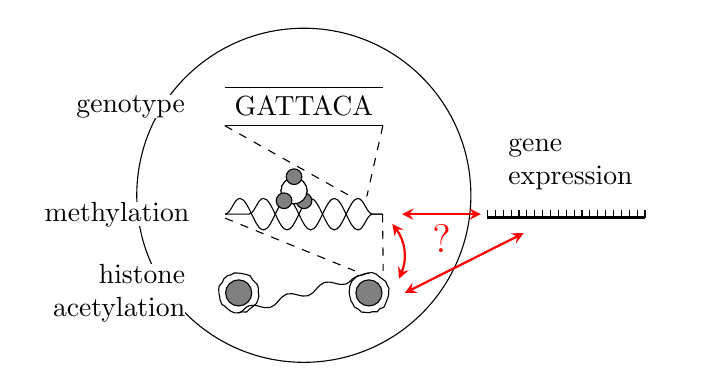
\begin{tikzpicture}
    \node (g) {GATTACA};
    \draw (g.north west) -- (g.north east);
    \draw (g.south west) -- (g.south east);

    \node [below left= of g.south] (m1) {};
    \node [below right= of g.south] (m2) {};
    \draw [decorate, decoration={snake, segment length=6mm, amplitude=2mm}] (m1) -- (m2);
    \draw [decorate, decoration={snake, segment length=6mm, amplitude=2mm, pre length=3mm}] (m1) -- (m2);
    \node [right=1cm of m1.north, anchor=south, circle, draw, fill=white] (me) { };
    \node [below right=-0.1 of me.south east, anchor=north west, circle, draw, fill=gray, inner sep=2pt] { };
    \node [right=1cm of m1.north, anchor=south, circle, draw, fill=white] (me) { };
    \node [below left=-0.1 of me.south west, anchor=north east, circle, draw, fill=gray, inner sep=2pt] { };
    \node [above=-0.1 of me.north, anchor=south, circle, draw, fill=gray, inner sep=2pt] { };

    \node [below= of m1.east, anchor=west, circle, draw, fill=gray] (a1) { };
    \node [below= of m2.west, anchor=east, circle, draw, fill=gray] (a2) { };
    \node [above=0 of a1.center, anchor=center, circle, draw, decorate,
           decoration={random steps, amplitude=0.1mm, segment length=0.5mm}, 
           inner sep=5pt] (a1out) { };
    \node [above=0 of a2.center, anchor=center, circle, draw, decorate,
           decoration={random steps, amplitude=0.1mm, segment length=0.5mm}, 
           inner sep=5pt] (a2out) { };
    \draw [decorate, decoration={snake, amplitude=0.5mm, segment length=5mm}]
          (a1out.south) -- (a2out.north);

    \draw [dashed] (g.south west) -- ($(m2.north west) + (-4mm, 1mm)$);
    \draw [dashed] (g.south east) -- ($(m2.north west) + (-2mm, 1mm)$);

    \draw [dashed] (m1) -- ($(a2out.north west) + (0mm, 1mm)$);
    \draw [dashed] (m2.west) -- ($(a2out.north east) + (0mm, 1mm)$);

    \node [circle, draw, above=of g.center, anchor=north, inner sep=1.5cm] { };

    \node [right=1cm of m2, inner sep=1pt] (e1) { };
    \node [right=2cm of e1, inner sep=1pt] (e2) { };
    \draw [decorate, decoration={ticks, amplitude=0.5mm, segment length=1mm}] (e1) -- (e2);
    \draw [thick] (e1.south east) -- (e2.south west);

    \draw [<->, >=stealth, thick, color=red] (e1) -- node [auto, color=red] {\Large{?}} (m2);
    \draw [<->, >=stealth, thick, color=red] ($(e1.south) + (5mm, -2mm)$) -- 
    ($(a2out.east) + (2mm, 0mm)$);
    \path [bend left, draw, <->, >=stealth, thick, color=red] (m2.south) to 
    ($(a2out.north east) + (2mm, 0)$);

    \node [above right=2mm of e1, text width=2cm] {gene \\ expression};
    \node [left=2mm of m1, fill=white, inner sep=0pt, align=right] {methylation};
    \node [left=5mm of a1, fill=white, inner sep=0pt, text width=2cm,
    align=right] {histone \\ acetylation};
    \node [left=5mm of g.west, fill=white, inner sep=0pt, align=right] {genotype};
\end{tikzpicture}
\end{document}

    \end{center}
        \uncover<3->{
        \item \textbf{how do these data fit together?}
        }
    \end{itemize}
\end{frame}

\begin{frame}{The data}
    \begin{columns}
        \begin{column}{0.35\textwidth}
            \begin{itemize}
                \item large cohort designed to study cognitive decline and
                    Alzheimer's disease
                \uncover<2->{
                \item genotype, gene expression, DNA methylation, and histone
                    acetylation (CHiP-seq) data 
                }
                \uncover<3->{
                \item 392 individuals with all four data types were used for
                    this analysis
                }
            \end{itemize}
        \end{column}
        \begin{column}{0.7\textwidth}
            % Created by tikzDevice version 0.7.0 on 2015-03-23 23:45:59
% !TEX encoding = UTF-8 Unicode
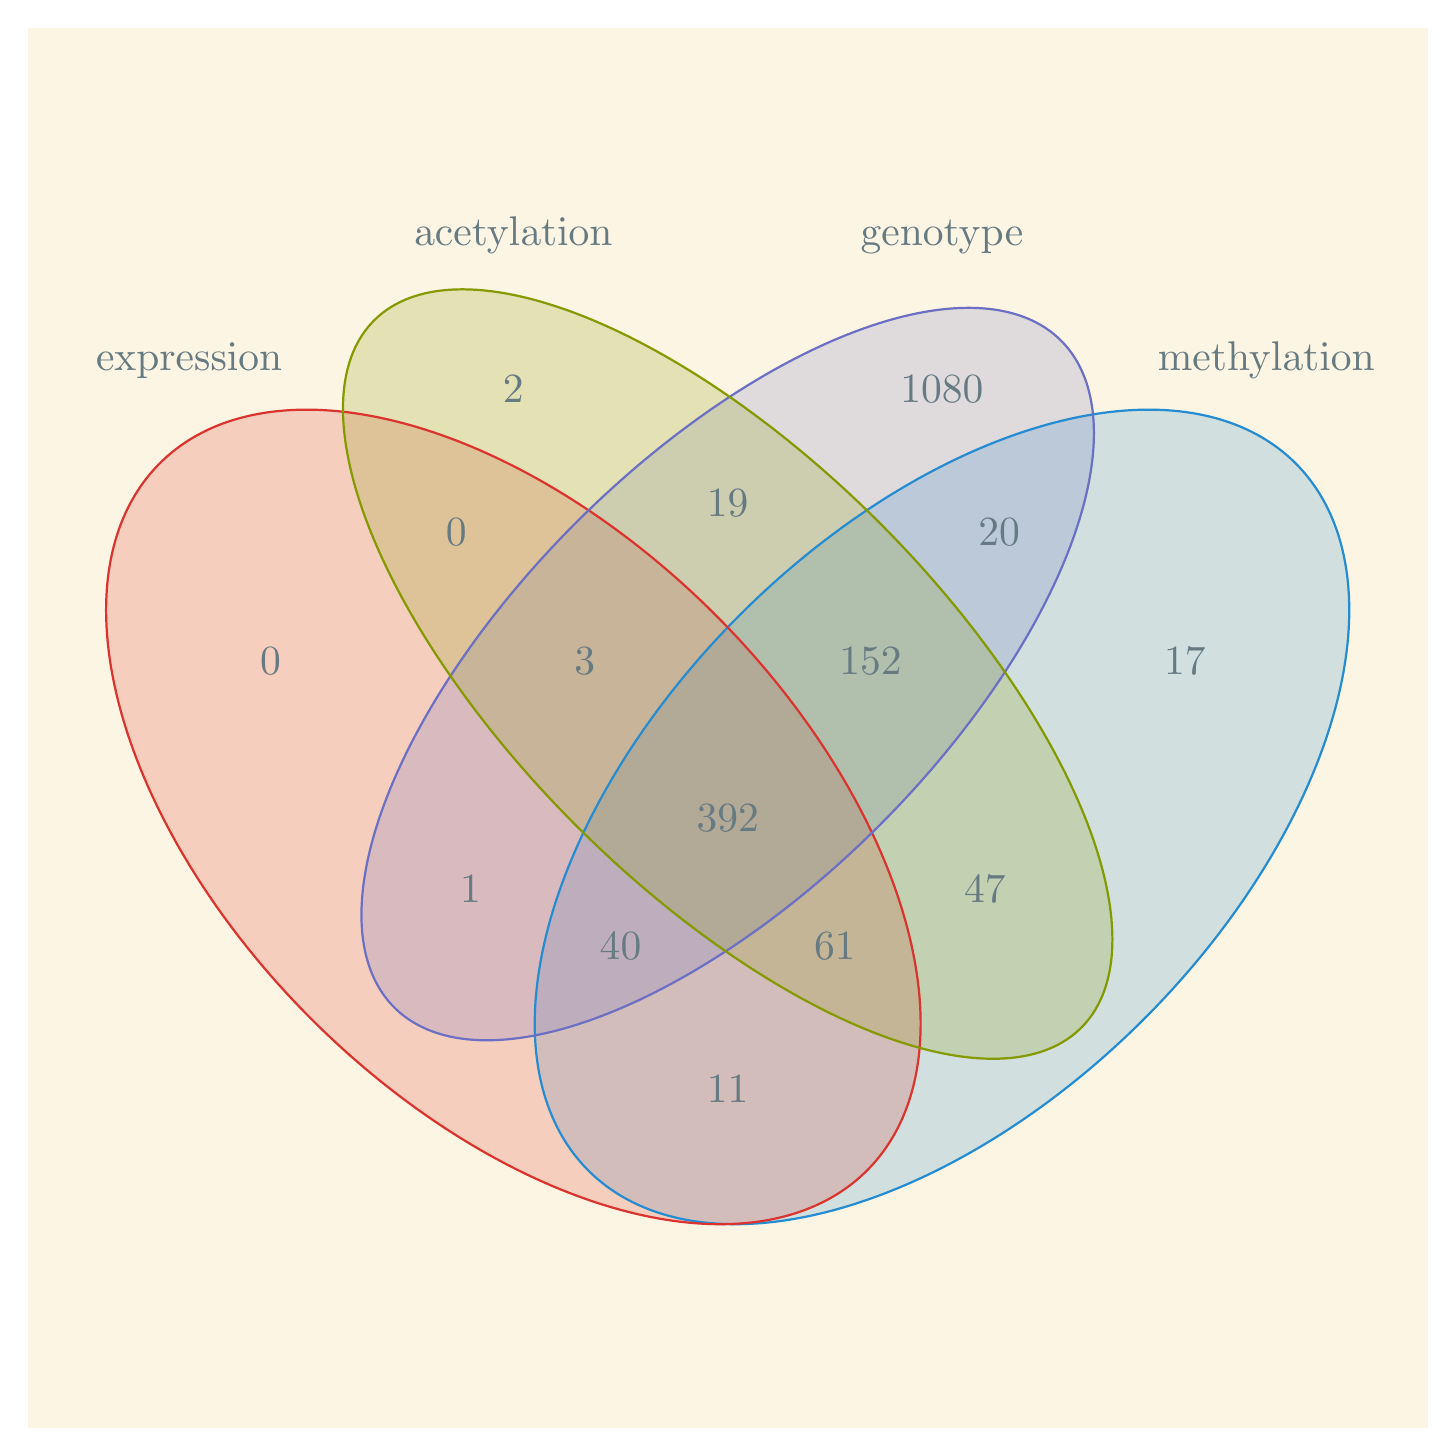
\begin{tikzpicture}[x=1pt,y=1pt]
\definecolor[named]{fillColor}{rgb}{0.99,0.96,0.89}
\path[use as bounding box,fill=fillColor] (0,0) rectangle (505.89,505.89);
\begin{scope}
\path[clip] (  0.00,  0.00) rectangle (505.89,505.89);
\definecolor[named]{fillColor}{rgb}{0.15,0.55,0.82}

\path[fill=fillColor,fill opacity=0.20] (458.16,348.46) --
	(458.00,348.61) --
	(457.85,348.77) --
	(457.70,348.92) --
	(457.54,349.07) --
	(457.39,349.22) --
	(457.23,349.37) --
	(457.07,349.52) --
	(456.92,349.67) --
	(456.76,349.81) --
	(456.60,349.96) --
	(456.44,350.11) --
	(456.28,350.25) --
	(456.12,350.40) --
	(455.96,350.55) --
	(455.80,350.69) --
	(455.64,350.83) --
	(455.48,350.98) --
	(455.31,351.12) --
	(455.15,351.26) --
	(454.99,351.41) --
	(454.82,351.55) --
	(454.66,351.69) --
	(454.49,351.83) --
	(454.33,351.97) --
	(454.16,352.11) --
	(453.99,352.24) --
	(453.83,352.38) --
	(453.66,352.52) --
	(453.49,352.66) --
	(453.32,352.79) --
	(453.15,352.93) --
	(452.98,353.06) --
	(452.81,353.20) --
	(452.64,353.33) --
	(452.47,353.46) --
	(452.29,353.60) --
	(452.12,353.73) --
	(451.95,353.86) --
	(451.77,353.99) --
	(451.60,354.12) --
	(451.42,354.25) --
	(451.25,354.38) --
	(451.07,354.51) --
	(450.90,354.64) --
	(450.72,354.76) --
	(450.54,354.89) --
	(450.36,355.02) --
	(450.18,355.14) --
	(450.01,355.27) --
	(449.83,355.39) --
	(449.65,355.52) --
	(449.46,355.64) --
	(449.28,355.76) --
	(449.10,355.88) --
	(448.92,356.01) --
	(448.74,356.13) --
	(448.55,356.25) --
	(448.37,356.37) --
	(448.18,356.49) --
	(448.00,356.60) --
	(447.81,356.72) --
	(447.63,356.84) --
	(447.44,356.96) --
	(447.25,357.07) --
	(447.07,357.19) --
	(446.88,357.30) --
	(446.69,357.42) --
	(446.50,357.53) --
	(446.31,357.64) --
	(446.12,357.76) --
	(445.93,357.87) --
	(445.74,357.98) --
	(445.55,358.09) --
	(445.36,358.20) --
	(445.16,358.31) --
	(444.97,358.42) --
	(444.78,358.53) --
	(444.58,358.63) --
	(444.39,358.74) --
	(444.19,358.85) --
	(444.00,358.95) --
	(443.80,359.06) --
	(443.60,359.16) --
	(443.41,359.27) --
	(443.21,359.37) --
	(443.01,359.47) --
	(442.81,359.58) --
	(442.61,359.68) --
	(442.41,359.78) --
	(442.21,359.88) --
	(442.01,359.98) --
	(441.81,360.08) --
	(441.61,360.18) --
	(441.41,360.27) --
	(441.21,360.37) --
	(441.00,360.47) --
	(440.80,360.56) --
	(440.59,360.66) --
	(440.39,360.75) --
	(440.19,360.85) --
	(439.98,360.94) --
	(439.77,361.04) --
	(439.57,361.13) --
	(439.36,361.22) --
	(439.15,361.31) --
	(438.95,361.40) --
	(438.74,361.49) --
	(438.53,361.58) --
	(438.32,361.67) --
	(438.11,361.76) --
	(437.90,361.84) --
	(437.69,361.93) --
	(437.48,362.02) --
	(437.27,362.10) --
	(437.05,362.19) --
	(436.84,362.27) --
	(436.63,362.36) --
	(436.41,362.44) --
	(436.20,362.52) --
	(435.99,362.60) --
	(435.77,362.68) --
	(435.56,362.77) --
	(435.34,362.85) --
	(435.12,362.92) --
	(434.91,363.00) --
	(434.69,363.08) --
	(434.47,363.16) --
	(434.25,363.24) --
	(434.04,363.31) --
	(433.82,363.39) --
	(433.60,363.46) --
	(433.38,363.54) --
	(433.16,363.61) --
	(432.94,363.68) --
	(432.71,363.76) --
	(432.49,363.83) --
	(432.27,363.90) --
	(432.05,363.97) --
	(431.82,364.04) --
	(431.60,364.11) --
	(431.38,364.18) --
	(431.15,364.25) --
	(430.93,364.31) --
	(430.70,364.38) --
	(430.48,364.45) --
	(430.25,364.51) --
	(430.02,364.58) --
	(429.80,364.64) --
	(429.57,364.71) --
	(429.34,364.77) --
	(429.11,364.83) --
	(428.88,364.89) --
	(428.66,364.95) --
	(428.43,365.01) --
	(428.20,365.07) --
	(427.97,365.13) --
	(427.73,365.19) --
	(427.50,365.25) --
	(427.27,365.31) --
	(427.04,365.36) --
	(426.81,365.42) --
	(426.57,365.48) --
	(426.34,365.53) --
	(426.11,365.59) --
	(425.87,365.64) --
	(425.64,365.69) --
	(425.40,365.74) --
	(425.17,365.80) --
	(424.93,365.85) --
	(424.69,365.90) --
	(424.46,365.95) --
	(424.22,366.00) --
	(423.98,366.04) --
	(423.74,366.09) --
	(423.51,366.14) --
	(423.27,366.19) --
	(423.03,366.23) --
	(422.79,366.28) --
	(422.55,366.32) --
	(422.31,366.37) --
	(422.07,366.41) --
	(421.83,366.45) --
	(421.58,366.49) --
	(421.34,366.54) --
	(421.10,366.58) --
	(420.86,366.62) --
	(420.61,366.66) --
	(420.37,366.69) --
	(420.12,366.73) --
	(419.88,366.77) --
	(419.64,366.81) --
	(419.39,366.84) --
	(419.14,366.88) --
	(418.90,366.91) --
	(418.65,366.95) --
	(418.41,366.98) --
	(418.16,367.02) --
	(417.91,367.05) --
	(417.66,367.08) --
	(417.41,367.11) --
	(417.17,367.14) --
	(416.92,367.17) --
	(416.67,367.20) --
	(416.42,367.23) --
	(416.17,367.26) --
	(415.92,367.28) --
	(415.67,367.31) --
	(415.41,367.34) --
	(415.16,367.36) --
	(414.91,367.39) --
	(414.66,367.41) --
	(414.40,367.43) --
	(414.15,367.46) --
	(413.90,367.48) --
	(413.64,367.50) --
	(413.39,367.52) --
	(413.13,367.54) --
	(412.88,367.56) --
	(412.62,367.58) --
	(412.37,367.60) --
	(412.11,367.62) --
	(411.86,367.63) --
	(411.60,367.65) --
	(411.34,367.67) --
	(411.08,367.68) --
	(410.83,367.70) --
	(410.57,367.71) --
	(410.31,367.72) --
	(410.05,367.73) --
	(409.79,367.75) --
	(409.53,367.76) --
	(409.27,367.77) --
	(409.01,367.78) --
	(408.75,367.79) --
	(408.49,367.80) --
	(408.23,367.80) --
	(407.97,367.81) --
	(407.70,367.82) --
	(407.44,367.82) --
	(407.18,367.83) --
	(406.92,367.83) --
	(406.65,367.84) --
	(406.39,367.84) --
	(406.12,367.85) --
	(405.86,367.85) --
	(405.60,367.85) --
	(405.33,367.85) --
	(405.07,367.85) --
	(404.80,367.85) --
	(404.53,367.85) --
	(404.27,367.85) --
	(404.00,367.84) --
	(403.73,367.84) --
	(403.47,367.84) --
	(403.20,367.83) --
	(402.93,367.83) --
	(402.66,367.82) --
	(402.39,367.82) --
	(402.12,367.81) --
	(401.85,367.80) --
	(401.59,367.79) --
	(401.32,367.79) --
	(401.05,367.78) --
	(400.77,367.77) --
	(400.50,367.76) --
	(400.23,367.74) --
	(399.96,367.73) --
	(399.69,367.72) --
	(399.42,367.71) --
	(399.15,367.69) --
	(398.87,367.68) --
	(398.60,367.66) --
	(398.33,367.65) --
	(398.05,367.63) --
	(397.78,367.61) --
	(397.50,367.59) --
	(397.23,367.58) --
	(396.96,367.56) --
	(396.68,367.54) --
	(396.41,367.52) --
	(396.13,367.50) --
	(395.85,367.47) --
	(395.58,367.45) --
	(395.30,367.43) --
	(395.02,367.41) --
	(394.75,367.38) --
	(394.47,367.36) --
	(394.19,367.33) --
	(393.91,367.30) --
	(393.64,367.28) --
	(393.36,367.25) --
	(393.08,367.22) --
	(392.80,367.19) --
	(392.52,367.16) --
	(392.24,367.13) --
	(391.96,367.10) --
	(391.68,367.07) --
	(391.40,367.04) --
	(391.12,367.01) --
	(390.84,366.97) --
	(390.56,366.94) --
	(390.28,366.91) --
	(390.00,366.87) --
	(389.71,366.83) --
	(389.43,366.80) --
	(389.15,366.76) --
	(388.87,366.72) --
	(388.58,366.68) --
	(388.30,366.65) --
	(388.02,366.61) --
	(387.73,366.57) --
	(387.45,366.52) --
	(387.16,366.48) --
	(386.88,366.44) --
	(386.60,366.40) --
	(386.31,366.35) --
	(386.03,366.31) --
	(385.74,366.27) --
	(385.45,366.22) --
	(385.17,366.17) --
	(384.88,366.13) --
	(384.60,366.08) --
	(384.31,366.03) --
	(384.02,365.98) --
	(383.74,365.93) --
	(383.45,365.88) --
	(383.16,365.83) --
	(382.87,365.78) --
	(382.58,365.73) --
	(382.30,365.68) --
	(382.01,365.63) --
	(381.72,365.57) --
	(381.43,365.52) --
	(381.14,365.46) --
	(380.85,365.41) --
	(380.56,365.35) --
	(380.27,365.29) --
	(379.98,365.24) --
	(379.69,365.18) --
	(379.40,365.12) --
	(379.11,365.06) --
	(378.82,365.00) --
	(378.53,364.94) --
	(378.24,364.88) --
	(377.94,364.82) --
	(377.65,364.75) --
	(377.36,364.69) --
	(377.07,364.63) --
	(376.78,364.56) --
	(376.48,364.50) --
	(376.19,364.43) --
	(375.90,364.36) --
	(375.61,364.30) --
	(375.31,364.23) --
	(375.02,364.16) --
	(374.72,364.09) --
	(374.43,364.02) --
	(374.14,363.95) --
	(373.84,363.88) --
	(373.55,363.81) --
	(373.25,363.74) --
	(372.96,363.67) --
	(372.66,363.59) --
	(372.37,363.52) --
	(372.07,363.44) --
	(371.78,363.37) --
	(371.48,363.29) --
	(371.18,363.22) --
	(370.89,363.14) --
	(370.59,363.06) --
	(370.29,362.98) --
	(370.00,362.91) --
	(369.70,362.83) --
	(369.40,362.75) --
	(369.11,362.66) --
	(368.81,362.58) --
	(368.51,362.50) --
	(368.21,362.42) --
	(367.92,362.34) --
	(367.62,362.25) --
	(367.32,362.17) --
	(367.02,362.08) --
	(366.72,362.00) --
	(366.42,361.91) --
	(366.12,361.82) --
	(365.83,361.73) --
	(365.53,361.65) --
	(365.23,361.56) --
	(364.93,361.47) --
	(364.63,361.38) --
	(364.33,361.29) --
	(364.03,361.20) --
	(363.73,361.10) --
	(363.43,361.01) --
	(363.13,360.92) --
	(362.83,360.82) --
	(362.53,360.73) --
	(362.23,360.64) --
	(361.92,360.54) --
	(361.62,360.44) --
	(361.32,360.35) --
	(361.02,360.25) --
	(360.72,360.15) --
	(360.42,360.05) --
	(360.12,359.95) --
	(359.81,359.85) --
	(359.51,359.75) --
	(359.21,359.65) --
	(358.91,359.55) --
	(358.60,359.45) --
	(358.30,359.34) --
	(358.00,359.24) --
	(357.70,359.14) --
	(357.39,359.03) --
	(357.09,358.93) --
	(356.79,358.82) --
	(356.48,358.71) --
	(356.18,358.61) --
	(355.88,358.50) --
	(355.57,358.39) --
	(355.27,358.28) --
	(354.97,358.17) --
	(354.66,358.06) --
	(354.36,357.95) --
	(354.05,357.84) --
	(353.75,357.73) --
	(353.45,357.61) --
	(353.14,357.50) --
	(352.84,357.39) --
	(352.53,357.27) --
	(352.23,357.16) --
	(351.92,357.04) --
	(351.62,356.93) --
	(351.31,356.81) --
	(351.01,356.69) --
	(350.70,356.57) --
	(350.40,356.46) --
	(350.09,356.34) --
	(349.79,356.22) --
	(349.48,356.10) --
	(349.17,355.97) --
	(348.87,355.85) --
	(348.56,355.73) --
	(348.26,355.61) --
	(347.95,355.49) --
	(347.65,355.36) --
	(347.34,355.24) --
	(347.03,355.11) --
	(346.73,354.99) --
	(346.42,354.86) --
	(346.11,354.73) --
	(345.81,354.60) --
	(345.50,354.48) --
	(345.19,354.35) --
	(344.89,354.22) --
	(344.58,354.09) --
	(344.27,353.96) --
	(343.97,353.83) --
	(343.66,353.70) --
	(343.35,353.56) --
	(343.05,353.43) --
	(342.74,353.30) --
	(342.43,353.16) --
	(342.12,353.03) --
	(341.82,352.89) --
	(341.51,352.76) --
	(341.20,352.62) --
	(340.90,352.49) --
	(340.59,352.35) --
	(340.28,352.21) --
	(339.97,352.07) --
	(339.67,351.93) --
	(339.36,351.79) --
	(339.05,351.65) --
	(338.74,351.51) --
	(338.43,351.37) --
	(338.13,351.23) --
	(337.82,351.09) --
	(337.51,350.94) --
	(337.20,350.80) --
	(336.90,350.65) --
	(336.59,350.51) --
	(336.28,350.36) --
	(335.97,350.22) --
	(335.66,350.07) --
	(335.36,349.92) --
	(335.05,349.78) --
	(334.74,349.63) --
	(334.43,349.48) --
	(334.12,349.33) --
	(333.81,349.18) --
	(333.51,349.03) --
	(333.20,348.88) --
	(332.89,348.73) --
	(332.58,348.57) --
	(332.27,348.42) --
	(331.97,348.27) --
	(331.66,348.11) --
	(331.35,347.96) --
	(331.04,347.81) --
	(330.73,347.65) --
	(330.42,347.49) --
	(330.12,347.34) --
	(329.81,347.18) --
	(329.50,347.02) --
	(329.19,346.86) --
	(328.88,346.70) --
	(328.58,346.55) --
	(328.27,346.39) --
	(327.96,346.22) --
	(327.65,346.06) --
	(327.34,345.90) --
	(327.03,345.74) --
	(326.73,345.58) --
	(326.42,345.41) --
	(326.11,345.25) --
	(325.80,345.09) --
	(325.49,344.92) --
	(325.19,344.75) --
	(324.88,344.59) --
	(324.57,344.42) --
	(324.26,344.26) --
	(323.95,344.09) --
	(323.65,343.92) --
	(323.34,343.75) --
	(323.03,343.58) --
	(322.72,343.41) --
	(322.42,343.24) --
	(322.11,343.07) --
	(321.80,342.90) --
	(321.49,342.73) --
	(321.18,342.55) --
	(320.88,342.38) --
	(320.57,342.21) --
	(320.26,342.03) --
	(319.95,341.86) --
	(319.65,341.68) --
	(319.34,341.51) --
	(319.03,341.33) --
	(318.73,341.15) --
	(318.42,340.98) --
	(318.11,340.80) --
	(317.80,340.62) --
	(317.50,340.44) --
	(317.19,340.26) --
	(316.88,340.08) --
	(316.58,339.90) --
	(316.27,339.72) --
	(315.96,339.54) --
	(315.66,339.36) --
	(315.35,339.18) --
	(315.04,338.99) --
	(314.74,338.81) --
	(314.43,338.63) --
	(314.12,338.44) --
	(313.82,338.26) --
	(313.51,338.07) --
	(313.20,337.88) --
	(312.90,337.70) --
	(312.59,337.51) --
	(312.29,337.32) --
	(311.98,337.13) --
	(311.67,336.95) --
	(311.37,336.76) --
	(311.06,336.57) --
	(310.76,336.38) --
	(310.45,336.19) --
	(310.15,335.99) --
	(309.84,335.80) --
	(309.54,335.61) --
	(309.23,335.42) --
	(308.93,335.22) --
	(308.62,335.03) --
	(308.32,334.84) --
	(308.01,334.64) --
	(307.71,334.45) --
	(307.40,334.25) --
	(307.10,334.05) --
	(306.79,333.86) --
	(306.49,333.66) --
	(306.19,333.46) --
	(305.88,333.26) --
	(305.58,333.06) --
	(305.27,332.87) --
	(304.97,332.67) --
	(304.67,332.47) --
	(304.36,332.26) --
	(304.06,332.06) --
	(303.76,331.86) --
	(303.45,331.66) --
	(303.15,331.46) --
	(302.85,331.25) --
	(302.55,331.05) --
	(302.24,330.85) --
	(301.94,330.64) --
	(301.64,330.44) --
	(301.34,330.23) --
	(301.03,330.02) --
	(300.73,329.82) --
	(300.43,329.61) --
	(300.13,329.40) --
	(299.83,329.20) --
	(299.53,328.99) --
	(299.22,328.78) --
	(298.92,328.57) --
	(298.62,328.36) --
	(298.32,328.15) --
	(298.02,327.94) --
	(297.72,327.73) --
	(297.42,327.52) --
	(297.12,327.30) --
	(296.82,327.09) --
	(296.52,326.88) --
	(296.22,326.66) --
	(295.92,326.45) --
	(295.62,326.23) --
	(295.32,326.02) --
	(295.02,325.80) --
	(294.72,325.59) --
	(294.42,325.37) --
	(294.12,325.16) --
	(293.83,324.94) --
	(293.53,324.72) --
	(293.23,324.50) --
	(292.93,324.28) --
	(292.63,324.06) --
	(292.34,323.84) --
	(292.04,323.62) --
	(291.74,323.40) --
	(291.44,323.18) --
	(291.15,322.96) --
	(290.85,322.74) --
	(290.55,322.52) --
	(290.26,322.29) --
	(289.96,322.07) --
	(289.66,321.85) --
	(289.37,321.62) --
	(289.07,321.40) --
	(288.78,321.17) --
	(288.48,320.95) --
	(288.18,320.72) --
	(287.89,320.50) --
	(287.59,320.27) --
	(287.30,320.04) --
	(287.00,319.82) --
	(286.71,319.59) --
	(286.42,319.36) --
	(286.12,319.13) --
	(285.83,318.90) --
	(285.53,318.67) --
	(285.24,318.44) --
	(284.95,318.21) --
	(284.65,317.98) --
	(284.36,317.75) --
	(284.07,317.52) --
	(283.78,317.28) --
	(283.48,317.05) --
	(283.19,316.82) --
	(282.90,316.58) --
	(282.61,316.35) --
	(282.32,316.12) --
	(282.03,315.88) --
	(281.74,315.65) --
	(281.44,315.41) --
	(281.15,315.17) --
	(280.86,314.94) --
	(280.57,314.70) --
	(280.28,314.46) --
	(279.99,314.23) --
	(279.70,313.99) --
	(279.42,313.75) --
	(279.13,313.51) --
	(278.84,313.27) --
	(278.55,313.03) --
	(278.26,312.79) --
	(277.97,312.55) --
	(277.68,312.31) --
	(277.40,312.07) --
	(277.11,311.83) --
	(276.82,311.58) --
	(276.54,311.34) --
	(276.25,311.10) --
	(275.96,310.85) --
	(275.68,310.61) --
	(275.39,310.37) --
	(275.10,310.12) --
	(274.82,309.88) --
	(274.53,309.63) --
	(274.25,309.39) --
	(273.96,309.14) --
	(273.68,308.89) --
	(273.39,308.65) --
	(273.11,308.40) --
	(272.83,308.15) --
	(272.54,307.90) --
	(272.26,307.65) --
	(271.98,307.41) --
	(271.69,307.16) --
	(271.41,306.91) --
	(271.13,306.66) --
	(270.85,306.41) --
	(270.57,306.16) --
	(270.28,305.90) --
	(270.00,305.65) --
	(269.72,305.40) --
	(269.44,305.15) --
	(269.16,304.90) --
	(268.88,304.64) --
	(268.60,304.39) --
	(268.32,304.14) --
	(268.04,303.88) --
	(267.76,303.63) --
	(267.48,303.37) --
	(267.21,303.12) --
	(266.93,302.86) --
	(266.65,302.61) --
	(266.37,302.35) --
	(266.09,302.09) --
	(265.82,301.84) --
	(265.54,301.58) --
	(265.26,301.32) --
	(264.99,301.06) --
	(264.71,300.81) --
	(264.44,300.55) --
	(264.16,300.29) --
	(263.89,300.03) --
	(263.61,299.77) --
	(263.34,299.51) --
	(263.06,299.25) --
	(262.79,298.99) --
	(262.51,298.73) --
	(262.24,298.47) --
	(261.97,298.20) --
	(261.70,297.94) --
	(261.42,297.68) --
	(261.15,297.42) --
	(260.88,297.15) --
	(260.61,296.89) --
	(260.34,296.63) --
	(260.07,296.36) --
	(259.80,296.10) --
	(259.52,295.83) --
	(259.25,295.57) --
	(258.99,295.30) --
	(258.72,295.04) --
	(258.45,294.77) --
	(258.18,294.50) --
	(257.91,294.24) --
	(257.64,293.97) --
	(257.37,293.70) --
	(257.11,293.43) --
	(256.84,293.17) --
	(256.57,292.90) --
	(256.31,292.63) --
	(256.04,292.36) --
	(255.77,292.09) --
	(255.51,291.82) --
	(255.24,291.55) --
	(254.98,291.28) --
	(254.71,291.01) --
	(254.45,290.74) --
	(254.19,290.47) --
	(253.92,290.20) --
	(253.66,289.92) --
	(253.40,289.65) --
	(253.13,289.38) --
	(252.87,289.11) --
	(252.61,288.83) --
	(252.35,288.56) --
	(252.09,288.29) --
	(251.83,288.01) --
	(251.57,287.74) --
	(251.31,287.46) --
	(251.05,287.19) --
	(250.79,286.91) --
	(250.53,286.64) --
	(250.27,286.36) --
	(250.01,286.09) --
	(249.75,285.81) --
	(249.50,285.53) --
	(249.24,285.26) --
	(248.98,284.98) --
	(248.72,284.70) --
	(248.47,284.43) --
	(248.21,284.15) --
	(247.96,283.87) --
	(247.70,283.59) --
	(247.45,283.31) --
	(247.19,283.03) --
	(246.94,282.75) --
	(246.68,282.47) --
	(246.43,282.19) --
	(246.18,281.91) --
	(245.93,281.63) --
	(245.67,281.35) --
	(245.42,281.07) --
	(245.17,280.79) --
	(244.92,280.51) --
	(244.67,280.23) --
	(244.42,279.95) --
	(244.17,279.66) --
	(243.92,279.38) --
	(243.67,279.10) --
	(243.42,278.82) --
	(243.17,278.53) --
	(242.92,278.25) --
	(242.68,277.96) --
	(242.43,277.68) --
	(242.18,277.40) --
	(241.94,277.11) --
	(241.69,276.83) --
	(241.44,276.54) --
	(241.20,276.26) --
	(240.95,275.97) --
	(240.71,275.69) --
	(240.46,275.40) --
	(240.22,275.11) --
	(239.98,274.83) --
	(239.73,274.54) --
	(239.49,274.25) --
	(239.25,273.97) --
	(239.01,273.68) --
	(238.77,273.39) --
	(238.53,273.10) --
	(238.28,272.81) --
	(238.04,272.53) --
	(237.81,272.24) --
	(237.57,271.95) --
	(237.33,271.66) --
	(237.09,271.37) --
	(236.85,271.08) --
	(236.61,270.79) --
	(236.37,270.50) --
	(236.14,270.21) --
	(235.90,269.92) --
	(235.67,269.63) --
	(235.43,269.34) --
	(235.19,269.05) --
	(234.96,268.76) --
	(234.73,268.47) --
	(234.49,268.17) --
	(234.26,267.88) --
	(234.02,267.59) --
	(233.79,267.30) --
	(233.56,267.01) --
	(233.33,266.71) --
	(233.10,266.42) --
	(232.87,266.13) --
	(232.63,265.83) --
	(232.40,265.54) --
	(232.17,265.25) --
	(231.95,264.95) --
	(231.72,264.66) --
	(231.49,264.36) --
	(231.26,264.07) --
	(231.03,263.78) --
	(230.81,263.48) --
	(230.58,263.19) --
	(230.35,262.89) --
	(230.13,262.60) --
	(229.90,262.30) --
	(229.68,262.00) --
	(229.45,261.71) --
	(229.23,261.41) --
	(229.00,261.12) --
	(228.78,260.82) --
	(228.56,260.52) --
	(228.34,260.23) --
	(228.11,259.93) --
	(227.89,259.63) --
	(227.67,259.33) --
	(227.45,259.04) --
	(227.23,258.74) --
	(227.01,258.44) --
	(226.79,258.14) --
	(226.57,257.85) --
	(226.36,257.55) --
	(226.14,257.25) --
	(225.92,256.95) --
	(225.70,256.65) --
	(225.49,256.35) --
	(225.27,256.05) --
	(225.06,255.75) --
	(224.84,255.45) --
	(224.63,255.16) --
	(224.41,254.86) --
	(224.20,254.56) --
	(223.99,254.26) --
	(223.77,253.96) --
	(223.56,253.66) --
	(223.35,253.35) --
	(223.14,253.05) --
	(222.93,252.75) --
	(222.72,252.45) --
	(222.51,252.15) --
	(222.30,251.85) --
	(222.09,251.55) --
	(221.88,251.25) --
	(221.67,250.95) --
	(221.46,250.64) --
	(221.26,250.34) --
	(221.05,250.04) --
	(220.84,249.74) --
	(220.64,249.44) --
	(220.43,249.13) --
	(220.23,248.83) --
	(220.02,248.53) --
	(219.82,248.23) --
	(219.62,247.92) --
	(219.42,247.62) --
	(219.21,247.32) --
	(219.01,247.01) --
	(218.81,246.71) --
	(218.61,246.41) --
	(218.41,246.10) --
	(218.21,245.80) --
	(218.01,245.50) --
	(217.81,245.19) --
	(217.61,244.89) --
	(217.42,244.58) --
	(217.22,244.28) --
	(217.02,243.98) --
	(216.83,243.67) --
	(216.63,243.37) --
	(216.43,243.06) --
	(216.24,242.76) --
	(216.05,242.45) --
	(215.85,242.15) --
	(215.66,241.84) --
	(215.47,241.54) --
	(215.27,241.23) --
	(215.08,240.93) --
	(214.89,240.62) --
	(214.70,240.32) --
	(214.51,240.01) --
	(214.32,239.71) --
	(214.13,239.40) --
	(213.94,239.09) --
	(213.75,238.79) --
	(213.57,238.48) --
	(213.38,238.18) --
	(213.19,237.87) --
	(213.01,237.56) --
	(212.82,237.26) --
	(212.63,236.95) --
	(212.45,236.65) --
	(212.27,236.34) --
	(212.08,236.03) --
	(211.90,235.73) --
	(211.72,235.42) --
	(211.53,235.11) --
	(211.35,234.81) --
	(211.17,234.50) --
	(210.99,234.19) --
	(210.81,233.89) --
	(210.63,233.58) --
	(210.45,233.27) --
	(210.28,232.96) --
	(210.10,232.66) --
	(209.92,232.35) --
	(209.74,232.04) --
	(209.57,231.74) --
	(209.39,231.43) --
	(209.22,231.12) --
	(209.04,230.81) --
	(208.87,230.51) --
	(208.69,230.20) --
	(208.52,229.89) --
	(208.35,229.58) --
	(208.18,229.28) --
	(208.01,228.97) --
	(207.83,228.66) --
	(207.66,228.35) --
	(207.49,228.04) --
	(207.32,227.74) --
	(207.16,227.43) --
	(206.99,227.12) --
	(206.82,226.81) --
	(206.65,226.50) --
	(206.49,226.20) --
	(206.32,225.89) --
	(206.15,225.58) --
	(205.99,225.27) --
	(205.83,224.96) --
	(205.66,224.66) --
	(205.50,224.35) --
	(205.34,224.04) --
	(205.17,223.73) --
	(205.01,223.42) --
	(204.85,223.12) --
	(204.69,222.81) --
	(204.53,222.50) --
	(204.37,222.19) --
	(204.21,221.88) --
	(204.05,221.57) --
	(203.90,221.27) --
	(203.74,220.96) --
	(203.58,220.65) --
	(203.43,220.34) --
	(203.27,220.03) --
	(203.12,219.73) --
	(202.96,219.42) --
	(202.81,219.11) --
	(202.65,218.80) --
	(202.50,218.49) --
	(202.35,218.18) --
	(202.20,217.88) --
	(202.05,217.57) --
	(201.90,217.26) --
	(201.75,216.95) --
	(201.60,216.64) --
	(201.45,216.34) --
	(201.30,216.03) --
	(201.15,215.72) --
	(201.00,215.41) --
	(200.86,215.10) --
	(200.71,214.80) --
	(200.57,214.49) --
	(200.42,214.18) --
	(200.28,213.87) --
	(200.13,213.56) --
	(199.99,213.26) --
	(199.85,212.95) --
	(199.71,212.64) --
	(199.56,212.33) --
	(199.42,212.03) --
	(199.28,211.72) --
	(199.14,211.41) --
	(199.00,211.10) --
	(198.87,210.80) --
	(198.73,210.49) --
	(198.59,210.18) --
	(198.45,209.87) --
	(198.32,209.57) --
	(198.18,209.26) --
	(198.05,208.95) --
	(197.91,208.64) --
	(197.78,208.34) --
	(197.64,208.03) --
	(197.51,207.72) --
	(197.38,207.42) --
	(197.25,207.11) --
	(197.12,206.80) --
	(196.99,206.49) --
	(196.86,206.19) --
	(196.73,205.88) --
	(196.60,205.57) --
	(196.47,205.27) --
	(196.34,204.96) --
	(196.22,204.66) --
	(196.09,204.35) --
	(195.96,204.04) --
	(195.84,203.74) --
	(195.71,203.43) --
	(195.59,203.12) --
	(195.47,202.82) --
	(195.34,202.51) --
	(195.22,202.21) --
	(195.10,201.90) --
	(194.98,201.60) --
	(194.86,201.29) --
	(194.74,200.98) --
	(194.62,200.68) --
	(194.50,200.37) --
	(194.38,200.07) --
	(194.27,199.76) --
	(194.15,199.46) --
	(194.03,199.15) --
	(193.92,198.85) --
	(193.80,198.54) --
	(193.69,198.24) --
	(193.57,197.93) --
	(193.46,197.63) --
	(193.35,197.33) --
	(193.24,197.02) --
	(193.12,196.72) --
	(193.01,196.41) --
	(192.90,196.11) --
	(192.79,195.81) --
	(192.68,195.50) --
	(192.58,195.20) --
	(192.47,194.89) --
	(192.36,194.59) --
	(192.25,194.29) --
	(192.15,193.98) --
	(192.04,193.68) --
	(191.94,193.38) --
	(191.83,193.08) --
	(191.73,192.77) --
	(191.63,192.47) --
	(191.53,192.17) --
	(191.42,191.87) --
	(191.32,191.56) --
	(191.22,191.26) --
	(191.12,190.96) --
	(191.02,190.66) --
	(190.92,190.36) --
	(190.83,190.05) --
	(190.73,189.75) --
	(190.63,189.45) --
	(190.54,189.15) --
	(190.44,188.85) --
	(190.34,188.55) --
	(190.25,188.25) --
	(190.16,187.95) --
	(190.06,187.65) --
	(189.97,187.35) --
	(189.88,187.05) --
	(189.79,186.75) --
	(189.70,186.45) --
	(189.61,186.15) --
	(189.52,185.85) --
	(189.43,185.55) --
	(189.34,185.25) --
	(189.25,184.95) --
	(189.17,184.65) --
	(189.08,184.35) --
	(188.99,184.05) --
	(188.91,183.76) --
	(188.82,183.46) --
	(188.74,183.16) --
	(188.66,182.86) --
	(188.57,182.56) --
	(188.49,182.27) --
	(188.41,181.97) --
	(188.33,181.67) --
	(188.25,181.37) --
	(188.17,181.08) --
	(188.09,180.78) --
	(188.01,180.48) --
	(187.94,180.19) --
	(187.86,179.89) --
	(187.78,179.60) --
	(187.71,179.30) --
	(187.63,179.00) --
	(187.56,178.71) --
	(187.48,178.41) --
	(187.41,178.12) --
	(187.34,177.82) --
	(187.26,177.53) --
	(187.19,177.23) --
	(187.12,176.94) --
	(187.05,176.65) --
	(186.98,176.35) --
	(186.91,176.06) --
	(186.85,175.76) --
	(186.78,175.47) --
	(186.71,175.18) --
	(186.64,174.88) --
	(186.58,174.59) --
	(186.51,174.30) --
	(186.45,174.01) --
	(186.39,173.71) --
	(186.32,173.42) --
	(186.26,173.13) --
	(186.20,172.84) --
	(186.14,172.55) --
	(186.08,172.26) --
	(186.02,171.97) --
	(185.96,171.67) --
	(185.90,171.38) --
	(185.84,171.09) --
	(185.78,170.80) --
	(185.72,170.51) --
	(185.67,170.22) --
	(185.61,169.93) --
	(185.56,169.65) --
	(185.50,169.36) --
	(185.45,169.07) --
	(185.40,168.78) --
	(185.34,168.49) --
	(185.29,168.20) --
	(185.24,167.92) --
	(185.19,167.63) --
	(185.14,167.34) --
	(185.09,167.05) --
	(185.04,166.77) --
	(185.00,166.48) --
	(184.95,166.19) --
	(184.90,165.91) --
	(184.86,165.62) --
	(184.81,165.34) --
	(184.76,165.05) --
	(184.72,164.76) --
	(184.68,164.48) --
	(184.63,164.20) --
	(184.59,163.91) --
	(184.55,163.63) --
	(184.51,163.34) --
	(184.47,163.06) --
	(184.43,162.78) --
	(184.39,162.49) --
	(184.35,162.21) --
	(184.31,161.93) --
	(184.28,161.64) --
	(184.24,161.36) --
	(184.21,161.08) --
	(184.17,160.80) --
	(184.14,160.52) --
	(184.10,160.24) --
	(184.07,159.95) --
	(184.04,159.67) --
	(184.00,159.39) --
	(183.97,159.11) --
	(183.94,158.83) --
	(183.91,158.55) --
	(183.88,158.28) --
	(183.85,158.00) --
	(183.83,157.72) --
	(183.80,157.44) --
	(183.77,157.16) --
	(183.74,156.88) --
	(183.72,156.61) --
	(183.69,156.33) --
	(183.67,156.05) --
	(183.65,155.77) --
	(183.62,155.50) --
	(183.60,155.22) --
	(183.58,154.95) --
	(183.56,154.67) --
	(183.54,154.39) --
	(183.52,154.12) --
	(183.50,153.85) --
	(183.48,153.57) --
	(183.46,153.30) --
	(183.45,153.02) --
	(183.43,152.75) --
	(183.41,152.48) --
	(183.40,152.20) --
	(183.38,151.93) --
	(183.37,151.66) --
	(183.36,151.39) --
	(183.34,151.11) --
	(183.33,150.84) --
	(183.32,150.57) --
	(183.31,150.30) --
	(183.30,150.03) --
	(183.29,149.76) --
	(183.28,149.49) --
	(183.27,149.22) --
	(183.27,148.95) --
	(183.26,148.68) --
	(183.25,148.41) --
	(183.25,148.15) --
	(183.24,147.88) --
	(183.24,147.61) --
	(183.23,147.34) --
	(183.23,147.08) --
	(183.23,146.81) --
	(183.23,146.54) --
	(183.23,146.28) --
	(183.23,146.01) --
	(183.23,145.74) --
	(183.23,145.48) --
	(183.23,145.22) --
	(183.23,144.95) --
	(183.23,144.69) --
	(183.24,144.42) --
	(183.24,144.16) --
	(183.25,143.90) --
	(183.25,143.63) --
	(183.26,143.37) --
	(183.26,143.11) --
	(183.27,142.85) --
	(183.28,142.59) --
	(183.29,142.32) --
	(183.30,142.06) --
	(183.31,141.80) --
	(183.32,141.54) --
	(183.33,141.28) --
	(183.34,141.02) --
	(183.35,140.77) --
	(183.37,140.51) --
	(183.38,140.25) --
	(183.39,139.99) --
	(183.41,139.73) --
	(183.43,139.48) --
	(183.44,139.22) --
	(183.46,138.96) --
	(183.48,138.71) --
	(183.49,138.45) --
	(183.51,138.20) --
	(183.53,137.94) --
	(183.55,137.69) --
	(183.57,137.43) --
	(183.60,137.18) --
	(183.62,136.92) --
	(183.64,136.67) --
	(183.66,136.42) --
	(183.69,136.17) --
	(183.71,135.91) --
	(183.74,135.66) --
	(183.76,135.41) --
	(183.79,135.16) --
	(183.82,134.91) --
	(183.85,134.66) --
	(183.87,134.41) --
	(183.90,134.16) --
	(183.93,133.91) --
	(183.96,133.66) --
	(184.00,133.41) --
	(184.03,133.16) --
	(184.06,132.92) --
	(184.09,132.67) --
	(184.13,132.42) --
	(184.16,132.18) --
	(184.20,131.93) --
	(184.23,131.69) --
	(184.27,131.44) --
	(184.31,131.19) --
	(184.34,130.95) --
	(184.38,130.71) --
	(184.42,130.46) --
	(184.46,130.22) --
	(184.50,129.98) --
	(184.54,129.73) --
	(184.58,129.49) --
	(184.62,129.25) --
	(184.67,129.01) --
	(184.71,128.77) --
	(184.75,128.53) --
	(184.80,128.29) --
	(184.84,128.05) --
	(184.89,127.81) --
	(184.94,127.57) --
	(184.98,127.33) --
	(185.03,127.09) --
	(185.08,126.86) --
	(185.13,126.62) --
	(185.18,126.38) --
	(185.23,126.15) --
	(185.28,125.91) --
	(185.33,125.67) --
	(185.38,125.44) --
	(185.44,125.20) --
	(185.49,124.97) --
	(185.54,124.74) --
	(185.60,124.50) --
	(185.65,124.27) --
	(185.71,124.04) --
	(185.77,123.80) --
	(185.82,123.57) --
	(185.88,123.34) --
	(185.94,123.11) --
	(186.00,122.88) --
	(186.06,122.65) --
	(186.12,122.42) --
	(186.18,122.19) --
	(186.24,121.96) --
	(186.31,121.73) --
	(186.37,121.51) --
	(186.43,121.28) --
	(186.50,121.05) --
	(186.56,120.82) --
	(186.63,120.60) --
	(186.69,120.37) --
	(186.76,120.15) --
	(186.83,119.92) --
	(186.90,119.70) --
	(186.97,119.47) --
	(187.03,119.25) --
	(187.10,119.03) --
	(187.18,118.80) --
	(187.25,118.58) --
	(187.32,118.36) --
	(187.39,118.14) --
	(187.46,117.92) --
	(187.54,117.70) --
	(187.61,117.48) --
	(187.69,117.26) --
	(187.76,117.04) --
	(187.84,116.82) --
	(187.92,116.60) --
	(187.99,116.39) --
	(188.07,116.17) --
	(188.15,115.95) --
	(188.23,115.74) --
	(188.31,115.52) --
	(188.39,115.30) --
	(188.47,115.09) --
	(188.55,114.88) --
	(188.64,114.66) --
	(188.72,114.45) --
	(188.80,114.23) --
	(188.89,114.02) --
	(188.97,113.81) --
	(189.06,113.60) --
	(189.14,113.39) --
	(189.23,113.18) --
	(189.32,112.97) --
	(189.41,112.76) --
	(189.50,112.55) --
	(189.58,112.34) --
	(189.67,112.13) --
	(189.76,111.92) --
	(189.86,111.71) --
	(189.95,111.51) --
	(190.04,111.30) --
	(190.13,111.10) --
	(190.23,110.89) --
	(190.32,110.69) --
	(190.42,110.48) --
	(190.51,110.28) --
	(190.61,110.07) --
	(190.70,109.87) --
	(190.80,109.67) --
	(190.90,109.47) --
	(191.00,109.26) --
	(191.10,109.06) --
	(191.20,108.86) --
	(191.30,108.66) --
	(191.40,108.46) --
	(191.50,108.26) --
	(191.60,108.06) --
	(191.70,107.87) --
	(191.81,107.67) --
	(191.91,107.47) --
	(192.02,107.28) --
	(192.12,107.08) --
	(192.23,106.88) --
	(192.33,106.69) --
	(192.44,106.49) --
	(192.55,106.30) --
	(192.66,106.11) --
	(192.77,105.91) --
	(192.88,105.72) --
	(192.99,105.53) --
	(193.10,105.34) --
	(193.21,105.15) --
	(193.32,104.95) --
	(193.43,104.76) --
	(193.55,104.57) --
	(193.66,104.39) --
	(193.77,104.20) --
	(193.89,104.01) --
	(194.00,103.82) --
	(194.12,103.63) --
	(194.24,103.45) --
	(194.35,103.26) --
	(194.47,103.08) --
	(194.59,102.89) --
	(194.71,102.71) --
	(194.83,102.52) --
	(194.95,102.34) --
	(195.07,102.16) --
	(195.19,101.97) --
	(195.31,101.79) --
	(195.44,101.61) --
	(195.56,101.43) --
	(195.68,101.25) --
	(195.81,101.07) --
	(195.93,100.89) --
	(196.06,100.71) --
	(196.18,100.53) --
	(196.31,100.36) --
	(196.44,100.18) --
	(196.57,100.00) --
	(196.69, 99.83) --
	(196.82, 99.65) --
	(196.95, 99.48) --
	(197.08, 99.30) --
	(197.21, 99.13) --
	(197.35, 98.95) --
	(197.48, 98.78) --
	(197.61, 98.61) --
	(197.74, 98.44) --
	(197.88, 98.27) --
	(198.01, 98.09) --
	(198.15, 97.92) --
	(198.28, 97.75) --
	(198.42, 97.59) --
	(198.56, 97.42) --
	(198.69, 97.25) --
	(198.83, 97.08) --
	(198.97, 96.91) --
	(199.11, 96.75) --
	(199.25, 96.58) --
	(199.39, 96.42) --
	(199.53, 96.25) --
	(199.67, 96.09) --
	(199.81, 95.92) --
	(199.95, 95.76) --
	(200.10, 95.60) --
	(200.24, 95.44) --
	(200.38, 95.27) --
	(200.53, 95.11) --
	(200.67, 94.95) --
	(200.82, 94.79) --
	(200.97, 94.63) --
	(201.11, 94.47) --
	(201.26, 94.32) --
	(201.41, 94.16) --
	(201.56, 94.00) --
	(201.71, 93.85) --
	(201.86, 93.69) --
	(202.01, 93.53) --
	(202.16, 93.38) --
	(202.31, 93.22) --
	(202.46, 93.07) --
	(202.61, 92.92) --
	(202.77, 92.77) --
	(202.92, 92.61) --
	(203.08, 92.46) --
	(203.23, 92.31) --
	(203.39, 92.16) --
	(203.54, 92.01) --
	(203.70, 91.86) --
	(203.86, 91.71) --
	(204.01, 91.56) --
	(204.17, 91.42) --
	(204.33, 91.27) --
	(204.49, 91.12) --
	(204.65, 90.98) --
	(204.81, 90.83) --
	(204.97, 90.69) --
	(205.13, 90.54) --
	(205.29, 90.40) --
	(205.46, 90.26) --
	(205.62, 90.11) --
	(205.78, 89.97) --
	(205.95, 89.83) --
	(206.11, 89.69) --
	(206.28, 89.55) --
	(206.44, 89.41) --
	(206.61, 89.27) --
	(206.78, 89.13) --
	(206.95, 89.00) --
	(207.11, 88.86) --
	(207.28, 88.72) --
	(207.45, 88.59) --
	(207.62, 88.45) --
	(207.79, 88.32) --
	(207.96, 88.18) --
	(208.13, 88.05) --
	(208.31, 87.91) --
	(208.48, 87.78) --
	(208.65, 87.65) --
	(208.82, 87.52) --
	(209.00, 87.39) --
	(209.17, 87.26) --
	(209.35, 87.13) --
	(209.52, 87.00) --
	(209.70, 86.87) --
	(209.88, 86.74) --
	(210.05, 86.61) --
	(210.23, 86.49) --
	(210.41, 86.36) --
	(210.59, 86.24) --
	(210.77, 86.11) --
	(210.95, 85.99) --
	(211.13, 85.86) --
	(211.31, 85.74) --
	(211.49, 85.62) --
	(211.67, 85.49) --
	(211.85, 85.37) --
	(212.04, 85.25) --
	(212.22, 85.13) --
	(212.40, 85.01) --
	(212.59, 84.89) --
	(212.77, 84.77) --
	(212.96, 84.66) --
	(213.14, 84.54) --
	(213.33, 84.42) --
	(213.52, 84.31) --
	(213.71, 84.19) --
	(213.89, 84.08) --
	(214.08, 83.96) --
	(214.27, 83.85) --
	(214.46, 83.74) --
	(214.65, 83.62) --
	(214.84, 83.51) --
	(215.03, 83.40) --
	(215.22, 83.29) --
	(215.42, 83.18) --
	(215.61, 83.07) --
	(215.80, 82.96) --
	(216.00, 82.85) --
	(216.19, 82.74) --
	(216.39, 82.64) --
	(216.58, 82.53) --
	(216.78, 82.43) --
	(216.97, 82.32) --
	(217.17, 82.22) --
	(217.37, 82.11) --
	(217.56, 82.01) --
	(217.76, 81.91) --
	(217.96, 81.80) --
	(218.16, 81.70) --
	(218.36, 81.60) --
	(218.56, 81.50) --
	(218.76, 81.40) --
	(218.96, 81.30) --
	(219.16, 81.20) --
	(219.36, 81.10) --
	(219.57, 81.01) --
	(219.77, 80.91) --
	(219.97, 80.81) --
	(220.18, 80.72) --
	(220.38, 80.62) --
	(220.59, 80.53) --
	(220.79, 80.44) --
	(221.00, 80.34) --
	(221.20, 80.25) --
	(221.41, 80.16) --
	(221.62, 80.07) --
	(221.83, 79.98) --
	(222.04, 79.89) --
	(222.24, 79.80) --
	(222.45, 79.71) --
	(222.66, 79.62) --
	(222.87, 79.53) --
	(223.08, 79.45) --
	(223.30, 79.36) --
	(223.51, 79.28) --
	(223.72, 79.19) --
	(223.93, 79.11) --
	(224.14, 79.02) --
	(224.36, 78.94) --
	(224.57, 78.86) --
	(224.79, 78.77) --
	(225.00, 78.69) --
	(225.22, 78.61) --
	(225.43, 78.53) --
	(225.65, 78.45) --
	(225.87, 78.37) --
	(226.08, 78.30) --
	(226.30, 78.22) --
	(226.52, 78.14) --
	(226.74, 78.07) --
	(226.96, 77.99) --
	(227.18, 77.92) --
	(227.40, 77.84) --
	(227.62, 77.77) --
	(227.84, 77.69) --
	(228.06, 77.62) --
	(228.28, 77.55) --
	(228.50, 77.48) --
	(228.72, 77.41) --
	(228.95, 77.34) --
	(229.17, 77.27) --
	(229.39, 77.20) --
	(229.62, 77.13) --
	(229.84, 77.06) --
	(230.07, 77.00) --
	(230.30, 76.93) --
	(230.52, 76.87) --
	(230.75, 76.80) --
	(230.97, 76.74) --
	(231.20, 76.67) --
	(231.43, 76.61) --
	(231.66, 76.55) --
	(231.89, 76.49) --
	(232.12, 76.42) --
	(232.35, 76.36) --
	(232.58, 76.30) --
	(232.81, 76.24) --
	(233.04, 76.19) --
	(233.27, 76.13) --
	(233.50, 76.07) --
	(233.73, 76.01) --
	(233.97, 75.96) --
	(234.20, 75.90) --
	(234.43, 75.85) --
	(234.67, 75.79) --
	(234.90, 75.74) --
	(235.14, 75.69) --
	(235.37, 75.63) --
	(235.61, 75.58) --
	(235.84, 75.53) --
	(236.08, 75.48) --
	(236.32, 75.43) --
	(236.55, 75.38) --
	(236.79, 75.33) --
	(237.03, 75.29) --
	(237.27, 75.24) --
	(237.51, 75.19) --
	(237.74, 75.15) --
	(237.98, 75.10) --
	(238.22, 75.06) --
	(238.46, 75.01) --
	(238.71, 74.97) --
	(238.95, 74.93) --
	(239.19, 74.88) --
	(239.43, 74.84) --
	(239.67, 74.80) --
	(239.92, 74.76) --
	(240.16, 74.72) --
	(240.40, 74.68) --
	(240.65, 74.65) --
	(240.89, 74.61) --
	(241.14, 74.57) --
	(241.38, 74.53) --
	(241.63, 74.50) --
	(241.87, 74.46) --
	(242.12, 74.43) --
	(242.37, 74.40) --
	(242.61, 74.36) --
	(242.86, 74.33) --
	(243.11, 74.30) --
	(243.36, 74.27) --
	(243.61, 74.24) --
	(243.86, 74.21) --
	(244.11, 74.18) --
	(244.36, 74.15) --
	(244.61, 74.12) --
	(244.86, 74.09) --
	(245.11, 74.07) --
	(245.36, 74.04) --
	(245.61, 74.02) --
	(245.86, 73.99) --
	(246.11, 73.97) --
	(246.37, 73.94) --
	(246.62, 73.92) --
	(246.87, 73.90) --
	(247.13, 73.88) --
	(247.38, 73.86) --
	(247.64, 73.84) --
	(247.89, 73.82) --
	(248.15, 73.80) --
	(248.40, 73.78) --
	(248.66, 73.76) --
	(248.92, 73.74) --
	(249.17, 73.73) --
	(249.43, 73.71) --
	(249.69, 73.70) --
	(249.95, 73.68) --
	(250.20, 73.67) --
	(250.46, 73.66) --
	(250.72, 73.64) --
	(250.98, 73.63) --
	(251.24, 73.62) --
	(251.50, 73.61) --
	(251.76, 73.60) --
	(252.02, 73.59) --
	(252.28, 73.58) --
	(252.54, 73.57) --
	(252.81, 73.57) --
	(253.07, 73.56) --
	(253.33, 73.55) --
	(253.59, 73.55) --
	(253.86, 73.54) --
	(254.12, 73.54) --
	(254.38, 73.54) --
	(254.65, 73.53) --
	(254.91, 73.53) --
	(255.18, 73.53) --
	(255.44, 73.53) --
	(255.71, 73.53) --
	(255.97, 73.53) --
	(256.24, 73.53) --
	(256.51, 73.53) --
	(256.77, 73.53) --
	(257.04, 73.54) --
	(257.31, 73.54) --
	(257.57, 73.54) --
	(257.84, 73.55) --
	(258.11, 73.56) --
	(258.38, 73.56) --
	(258.65, 73.57) --
	(258.92, 73.58) --
	(259.19, 73.58) --
	(259.46, 73.59) --
	(259.73, 73.60) --
	(260.00, 73.61) --
	(260.27, 73.62) --
	(260.54, 73.63) --
	(260.81, 73.65) --
	(261.08, 73.66) --
	(261.35, 73.67) --
	(261.63, 73.69) --
	(261.90, 73.70) --
	(262.17, 73.72) --
	(262.45, 73.73) --
	(262.72, 73.75) --
	(262.99, 73.77) --
	(263.27, 73.78) --
	(263.54, 73.80) --
	(263.82, 73.82) --
	(264.09, 73.84) --
	(264.37, 73.86) --
	(264.64, 73.88) --
	(264.92, 73.90) --
	(265.19, 73.93) --
	(265.47, 73.95) --
	(265.75, 73.97) --
	(266.02, 74.00) --
	(266.30, 74.02) --
	(266.58, 74.05) --
	(266.86, 74.07) --
	(267.14, 74.10) --
	(267.41, 74.13) --
	(267.69, 74.16) --
	(267.97, 74.19) --
	(268.25, 74.21) --
	(268.53, 74.24) --
	(268.81, 74.28) --
	(269.09, 74.31) --
	(269.37, 74.34) --
	(269.65, 74.37) --
	(269.93, 74.40) --
	(270.21, 74.44) --
	(270.49, 74.47) --
	(270.78, 74.51) --
	(271.06, 74.54) --
	(271.34, 74.58) --
	(271.62, 74.62) --
	(271.91, 74.66) --
	(272.19, 74.69) --
	(272.47, 74.73) --
	(272.76, 74.77) --
	(273.04, 74.81) --
	(273.32, 74.85) --
	(273.61, 74.90) --
	(273.89, 74.94) --
	(274.18, 74.98) --
	(274.46, 75.02) --
	(274.75, 75.07) --
	(275.03, 75.11) --
	(275.32, 75.16) --
	(275.60, 75.20) --
	(275.89, 75.25) --
	(276.18, 75.30) --
	(276.46, 75.35) --
	(276.75, 75.39) --
	(277.04, 75.44) --
	(277.32, 75.49) --
	(277.61, 75.54) --
	(277.90, 75.60) --
	(278.19, 75.65) --
	(278.48, 75.70) --
	(278.76, 75.75) --
	(279.05, 75.81) --
	(279.34, 75.86) --
	(279.63, 75.92) --
	(279.92, 75.97) --
	(280.21, 76.03) --
	(280.50, 76.08) --
	(280.79, 76.14) --
	(281.08, 76.20) --
	(281.37, 76.26) --
	(281.66, 76.32) --
	(281.95, 76.38) --
	(282.24, 76.44) --
	(282.54, 76.50) --
	(282.83, 76.56) --
	(283.12, 76.63) --
	(283.41, 76.69) --
	(283.70, 76.75) --
	(284.00, 76.82) --
	(284.29, 76.88) --
	(284.58, 76.95) --
	(284.87, 77.01) --
	(285.17, 77.08) --
	(285.46, 77.15) --
	(285.75, 77.22) --
	(286.05, 77.29) --
	(286.34, 77.36) --
	(286.64, 77.43) --
	(286.93, 77.50) --
	(287.23, 77.57) --
	(287.52, 77.64) --
	(287.81, 77.71) --
	(288.11, 77.79) --
	(288.41, 77.86) --
	(288.70, 77.93) --
	(289.00, 78.01) --
	(289.29, 78.09) --
	(289.59, 78.16) --
	(289.88, 78.24) --
	(290.18, 78.32) --
	(290.48, 78.39) --
	(290.77, 78.47) --
	(291.07, 78.55) --
	(291.37, 78.63) --
	(291.67, 78.71) --
	(291.96, 78.80) --
	(292.26, 78.88) --
	(292.56, 78.96) --
	(292.86, 79.04) --
	(293.15, 79.13) --
	(293.45, 79.21) --
	(293.75, 79.30) --
	(294.05, 79.38) --
	(294.35, 79.47) --
	(294.65, 79.56) --
	(294.95, 79.64) --
	(295.25, 79.73) --
	(295.55, 79.82) --
	(295.84, 79.91) --
	(296.14, 80.00) --
	(296.44, 80.09) --
	(296.74, 80.18) --
	(297.04, 80.27) --
	(297.34, 80.37) --
	(297.64, 80.46) --
	(297.95, 80.55) --
	(298.25, 80.65) --
	(298.55, 80.74) --
	(298.85, 80.84) --
	(299.15, 80.93) --
	(299.45, 81.03) --
	(299.75, 81.13) --
	(300.05, 81.23) --
	(300.35, 81.33) --
	(300.66, 81.43) --
	(300.96, 81.53) --
	(301.26, 81.63) --
	(301.56, 81.73) --
	(301.87, 81.83) --
	(302.17, 81.93) --
	(302.47, 82.03) --
	(302.77, 82.14) --
	(303.08, 82.24) --
	(303.38, 82.35) --
	(303.68, 82.45) --
	(303.98, 82.56) --
	(304.29, 82.66) --
	(304.59, 82.77) --
	(304.89, 82.88) --
	(305.20, 82.99) --
	(305.50, 83.10) --
	(305.81, 83.21) --
	(306.11, 83.32) --
	(306.41, 83.43) --
	(306.72, 83.54) --
	(307.02, 83.65) --
	(307.33, 83.76) --
	(307.63, 83.88) --
	(307.94, 83.99) --
	(308.24, 84.11) --
	(308.55, 84.22) --
	(308.85, 84.34) --
	(309.15, 84.45) --
	(309.46, 84.57) --
	(309.77, 84.69) --
	(310.07, 84.80) --
	(310.38, 84.92) --
	(310.68, 85.04) --
	(310.99, 85.16) --
	(311.29, 85.28) --
	(311.60, 85.40) --
	(311.90, 85.52) --
	(312.21, 85.65) --
	(312.52, 85.77) --
	(312.82, 85.89) --
	(313.13, 86.02) --
	(313.43, 86.14) --
	(313.74, 86.27) --
	(314.05, 86.39) --
	(314.35, 86.52) --
	(314.66, 86.65) --
	(314.97, 86.77) --
	(315.27, 86.90) --
	(315.58, 87.03) --
	(315.88, 87.16) --
	(316.19, 87.29) --
	(316.50, 87.42) --
	(316.81, 87.55) --
	(317.11, 87.68) --
	(317.42, 87.81) --
	(317.73, 87.95) --
	(318.03, 88.08) --
	(318.34, 88.21) --
	(318.65, 88.35) --
	(318.95, 88.48) --
	(319.26, 88.62) --
	(319.57, 88.76) --
	(319.88, 88.89) --
	(320.18, 89.03) --
	(320.49, 89.17) --
	(320.80, 89.31) --
	(321.11, 89.45) --
	(321.41, 89.59) --
	(321.72, 89.73) --
	(322.03, 89.87) --
	(322.34, 90.01) --
	(322.65, 90.15) --
	(322.95, 90.29) --
	(323.26, 90.44) --
	(323.57, 90.58) --
	(323.88, 90.72) --
	(324.18, 90.87) --
	(324.49, 91.01) --
	(324.80, 91.16) --
	(325.11, 91.31) --
	(325.42, 91.45) --
	(325.72, 91.60) --
	(326.03, 91.75) --
	(326.34, 91.90) --
	(326.65, 92.05) --
	(326.96, 92.20) --
	(327.27, 92.35) --
	(327.57, 92.50) --
	(327.88, 92.65) --
	(328.19, 92.80) --
	(328.50, 92.96) --
	(328.81, 93.11) --
	(329.11, 93.26) --
	(329.42, 93.42) --
	(329.73, 93.57) --
	(330.04, 93.73) --
	(330.35, 93.88) --
	(330.66, 94.04) --
	(330.96, 94.20) --
	(331.27, 94.36) --
	(331.58, 94.51) --
	(331.89, 94.67) --
	(332.20, 94.83) --
	(332.50, 94.99) --
	(332.81, 95.15) --
	(333.12, 95.31) --
	(333.43, 95.48) --
	(333.74, 95.64) --
	(334.05, 95.80) --
	(334.35, 95.96) --
	(334.66, 96.13) --
	(334.97, 96.29) --
	(335.28, 96.46) --
	(335.59, 96.62) --
	(335.89, 96.79) --
	(336.20, 96.96) --
	(336.51, 97.12) --
	(336.82, 97.29) --
	(337.13, 97.46) --
	(337.43, 97.63) --
	(337.74, 97.80) --
	(338.05, 97.97) --
	(338.36, 98.14) --
	(338.66, 98.31) --
	(338.97, 98.48) --
	(339.28, 98.65) --
	(339.59, 98.82) --
	(339.90, 99.00) --
	(340.20, 99.17) --
	(340.51, 99.34) --
	(340.82, 99.52) --
	(341.13, 99.69) --
	(341.43, 99.87) --
	(341.74,100.05) --
	(342.05,100.22) --
	(342.35,100.40) --
	(342.66,100.58) --
	(342.97,100.76) --
	(343.28,100.94) --
	(343.58,101.12) --
	(343.89,101.30) --
	(344.20,101.48) --
	(344.50,101.66) --
	(344.81,101.84) --
	(345.12,102.02) --
	(345.42,102.20) --
	(345.73,102.39) --
	(346.04,102.57) --
	(346.34,102.75) --
	(346.65,102.94) --
	(346.96,103.12) --
	(347.26,103.31) --
	(347.57,103.49) --
	(347.87,103.68) --
	(348.18,103.87) --
	(348.49,104.06) --
	(348.79,104.24) --
	(349.10,104.43) --
	(349.40,104.62) --
	(349.71,104.81) --
	(350.01,105.00) --
	(350.32,105.19) --
	(350.62,105.38) --
	(350.93,105.58) --
	(351.24,105.77) --
	(351.54,105.96) --
	(351.85,106.15) --
	(352.15,106.35) --
	(352.46,106.54) --
	(352.76,106.74) --
	(353.06,106.93) --
	(353.37,107.13) --
	(353.67,107.32) --
	(353.98,107.52) --
	(354.28,107.72) --
	(354.59,107.92) --
	(354.89,108.11) --
	(355.19,108.31) --
	(355.50,108.51) --
	(355.80,108.71) --
	(356.10,108.91) --
	(356.41,109.11) --
	(356.71,109.31) --
	(357.01,109.52) --
	(357.32,109.72) --
	(357.62,109.92) --
	(357.92,110.12) --
	(358.23,110.33) --
	(358.53,110.53) --
	(358.83,110.74) --
	(359.13,110.94) --
	(359.44,111.15) --
	(359.74,111.35) --
	(360.04,111.56) --
	(360.34,111.77) --
	(360.64,111.97) --
	(360.94,112.18) --
	(361.25,112.39) --
	(361.55,112.60) --
	(361.85,112.81) --
	(362.15,113.02) --
	(362.45,113.23) --
	(362.75,113.44) --
	(363.05,113.65) --
	(363.35,113.86) --
	(363.65,114.08) --
	(363.95,114.29) --
	(364.25,114.50) --
	(364.55,114.71) --
	(364.85,114.93) --
	(365.15,115.14) --
	(365.45,115.36) --
	(365.75,115.57) --
	(366.05,115.79) --
	(366.35,116.01) --
	(366.65,116.22) --
	(366.95,116.44) --
	(367.24,116.66) --
	(367.54,116.88) --
	(367.84,117.10) --
	(368.14,117.31) --
	(368.44,117.53) --
	(368.73,117.75) --
	(369.03,117.97) --
	(369.33,118.20) --
	(369.63,118.42) --
	(369.92,118.64) --
	(370.22,118.86) --
	(370.52,119.08) --
	(370.81,119.31) --
	(371.11,119.53) --
	(371.41,119.75) --
	(371.70,119.98) --
	(372.00,120.20) --
	(372.29,120.43) --
	(372.59,120.66) --
	(372.88,120.88) --
	(373.18,121.11) --
	(373.47,121.34) --
	(373.77,121.56) --
	(374.06,121.79) --
	(374.36,122.02) --
	(374.65,122.25) --
	(374.94,122.48) --
	(375.24,122.71) --
	(375.53,122.94) --
	(375.82,123.17) --
	(376.12,123.40) --
	(376.41,123.63) --
	(376.70,123.86) --
	(377.00,124.09) --
	(377.29,124.33) --
	(377.58,124.56) --
	(377.87,124.79) --
	(378.16,125.03) --
	(378.45,125.26) --
	(378.75,125.50) --
	(379.04,125.73) --
	(379.33,125.97) --
	(379.62,126.20) --
	(379.91,126.44) --
	(380.20,126.68) --
	(380.49,126.92) --
	(380.78,127.15) --
	(381.07,127.39) --
	(381.36,127.63) --
	(381.65,127.87) --
	(381.93,128.11) --
	(382.22,128.35) --
	(382.51,128.59) --
	(382.80,128.83) --
	(383.09,129.07) --
	(383.38,129.31) --
	(383.66,129.55) --
	(383.95,129.80) --
	(384.24,130.04) --
	(384.52,130.28) --
	(384.81,130.52) --
	(385.10,130.77) --
	(385.38,131.01) --
	(385.67,131.26) --
	(385.95,131.50) --
	(386.24,131.75) --
	(386.52,131.99) --
	(386.81,132.24) --
	(387.09,132.49) --
	(387.38,132.73) --
	(387.66,132.98) --
	(387.95,133.23) --
	(388.23,133.48) --
	(388.51,133.72) --
	(388.80,133.97) --
	(389.08,134.22) --
	(389.36,134.47) --
	(389.64,134.72) --
	(389.92,134.97) --
	(390.21,135.22) --
	(390.49,135.47) --
	(390.77,135.72) --
	(391.05,135.98) --
	(391.33,136.23) --
	(391.61,136.48) --
	(391.89,136.73) --
	(392.17,136.99) --
	(392.45,137.24) --
	(392.73,137.50) --
	(393.01,137.75) --
	(393.29,138.00) --
	(393.57,138.26) --
	(393.84,138.52) --
	(394.12,138.77) --
	(394.40,139.03) --
	(394.68,139.28) --
	(394.95,139.54) --
	(395.23,139.80) --
	(395.51,140.06) --
	(395.78,140.31) --
	(396.06,140.57) --
	(396.34,140.83) --
	(396.61,141.09) --
	(396.89,141.35) --
	(397.16,141.61) --
	(397.44,141.87) --
	(397.71,142.13) --
	(397.98,142.39) --
	(398.26,142.65) --
	(398.53,142.91) --
	(398.80,143.17) --
	(399.08,143.44) --
	(399.35,143.70) --
	(399.62,143.96) --
	(399.89,144.23) --
	(400.16,144.49) --
	(400.44,144.75) --
	(400.71,145.02) --
	(400.98,145.28) --
	(401.25,145.55) --
	(401.52,145.81) --
	(401.79,146.08) --
	(402.06,146.34) --
	(402.33,146.61) --
	(402.59,146.88) --
	(402.86,147.14) --
	(403.13,147.41) --
	(403.40,147.68) --
	(403.67,147.94) --
	(403.93,148.21) --
	(404.20,148.48) --
	(404.47,148.75) --
	(404.73,149.02) --
	(405.00,149.29) --
	(405.26,149.56) --
	(405.53,149.83) --
	(405.79,150.10) --
	(406.06,150.37) --
	(406.32,150.64) --
	(406.59,150.91) --
	(406.85,151.18) --
	(407.11,151.45) --
	(407.38,151.73) --
	(407.64,152.00) --
	(407.90,152.27) --
	(408.16,152.54) --
	(408.42,152.82) --
	(408.68,153.09) --
	(408.95,153.37) --
	(409.21,153.64) --
	(409.47,153.91) --
	(409.73,154.19) --
	(409.99,154.46) --
	(410.24,154.74) --
	(410.50,155.02) --
	(410.76,155.29) --
	(411.02,155.57) --
	(411.28,155.84) --
	(411.53,156.12) --
	(411.79,156.40) --
	(412.05,156.68) --
	(412.30,156.95) --
	(412.56,157.23) --
	(412.82,157.51) --
	(413.07,157.79) --
	(413.33,158.07) --
	(413.58,158.35) --
	(413.83,158.62) --
	(414.09,158.90) --
	(414.34,159.18) --
	(414.59,159.46) --
	(414.85,159.74) --
	(415.10,160.03) --
	(415.35,160.31) --
	(415.60,160.59) --
	(415.85,160.87) --
	(416.10,161.15) --
	(416.35,161.43) --
	(416.60,161.71) --
	(416.85,162.00) --
	(417.10,162.28) --
	(417.35,162.56) --
	(417.60,162.85) --
	(417.85,163.13) --
	(418.10,163.41) --
	(418.34,163.70) --
	(418.59,163.98) --
	(418.84,164.27) --
	(419.08,164.55) --
	(419.33,164.84) --
	(419.57,165.12) --
	(419.82,165.41) --
	(420.06,165.69) --
	(420.31,165.98) --
	(420.55,166.27) --
	(420.79,166.55) --
	(421.04,166.84) --
	(421.28,167.13) --
	(421.52,167.41) --
	(421.76,167.70) --
	(422.01,167.99) --
	(422.25,168.28) --
	(422.49,168.56) --
	(422.73,168.85) --
	(422.97,169.14) --
	(423.21,169.43) --
	(423.45,169.72) --
	(423.68,170.01) --
	(423.92,170.30) --
	(424.16,170.59) --
	(424.40,170.88) --
	(424.63,171.17) --
	(424.87,171.46) --
	(425.11,171.75) --
	(425.34,172.04) --
	(425.58,172.33) --
	(425.81,172.62) --
	(426.05,172.91) --
	(426.28,173.20) --
	(426.51,173.50) --
	(426.75,173.79) --
	(426.98,174.08) --
	(427.21,174.37) --
	(427.44,174.67) --
	(427.68,174.96) --
	(427.91,175.25) --
	(428.14,175.54) --
	(428.37,175.84) --
	(428.60,176.13) --
	(428.83,176.43) --
	(429.06,176.72) --
	(429.28,177.01) --
	(429.51,177.31) --
	(429.74,177.60) --
	(429.97,177.90) --
	(430.19,178.19) --
	(430.42,178.49) --
	(430.65,178.78) --
	(430.87,179.08) --
	(431.10,179.37) --
	(431.32,179.67) --
	(431.54,179.97) --
	(431.77,180.26) --
	(431.99,180.56) --
	(432.21,180.86) --
	(432.44,181.15) --
	(432.66,181.45) --
	(432.88,181.75) --
	(433.10,182.04) --
	(433.32,182.34) --
	(433.54,182.64) --
	(433.76,182.94) --
	(433.98,183.23) --
	(434.20,183.53) --
	(434.42,183.83) --
	(434.63,184.13) --
	(434.85,184.43) --
	(435.07,184.73) --
	(435.29,185.03) --
	(435.50,185.32) --
	(435.72,185.62) --
	(435.93,185.92) --
	(436.15,186.22) --
	(436.36,186.52) --
	(436.57,186.82) --
	(436.79,187.12) --
	(437.00,187.42) --
	(437.21,187.72) --
	(437.42,188.02) --
	(437.64,188.32) --
	(437.85,188.62) --
	(438.06,188.93) --
	(438.27,189.23) --
	(438.48,189.53) --
	(438.68,189.83) --
	(438.89,190.13) --
	(439.10,190.43) --
	(439.31,190.73) --
	(439.52,191.04) --
	(439.72,191.34) --
	(439.93,191.64) --
	(440.13,191.94) --
	(440.34,192.24) --
	(440.54,192.55) --
	(440.75,192.85) --
	(440.95,193.15) --
	(441.15,193.45) --
	(441.36,193.76) --
	(441.56,194.06) --
	(441.76,194.36) --
	(441.96,194.67) --
	(442.16,194.97) --
	(442.36,195.27) --
	(442.56,195.58) --
	(442.76,195.88) --
	(442.96,196.19) --
	(443.16,196.49) --
	(443.36,196.79) --
	(443.55,197.10) --
	(443.75,197.40) --
	(443.95,197.71) --
	(444.14,198.01) --
	(444.34,198.32) --
	(444.53,198.62) --
	(444.73,198.93) --
	(444.92,199.23) --
	(445.11,199.53) --
	(445.31,199.84) --
	(445.50,200.15) --
	(445.69,200.45) --
	(445.88,200.76) --
	(446.07,201.06) --
	(446.26,201.37) --
	(446.45,201.67) --
	(446.64,201.98) --
	(446.83,202.28) --
	(447.02,202.59) --
	(447.21,202.90) --
	(447.39,203.20) --
	(447.58,203.51) --
	(447.77,203.81) --
	(447.95,204.12) --
	(448.14,204.43) --
	(448.32,204.73) --
	(448.51,205.04) --
	(448.69,205.35) --
	(448.87,205.65) --
	(449.06,205.96) --
	(449.24,206.27) --
	(449.42,206.57) --
	(449.60,206.88) --
	(449.78,207.19) --
	(449.96,207.49) --
	(450.14,207.80) --
	(450.32,208.11) --
	(450.50,208.41) --
	(450.67,208.72) --
	(450.85,209.03) --
	(451.03,209.34) --
	(451.20,209.64) --
	(451.38,209.95) --
	(451.56,210.26) --
	(451.73,210.57) --
	(451.90,210.87) --
	(452.08,211.18) --
	(452.25,211.49) --
	(452.42,211.80) --
	(452.60,212.10) --
	(452.77,212.41) --
	(452.94,212.72) --
	(453.11,213.03) --
	(453.28,213.33) --
	(453.45,213.64) --
	(453.62,213.95) --
	(453.78,214.26) --
	(453.95,214.57) --
	(454.12,214.87) --
	(454.29,215.18) --
	(454.45,215.49) --
	(454.62,215.80) --
	(454.78,216.11) --
	(454.95,216.41) --
	(455.11,216.72) --
	(455.27,217.03) --
	(455.44,217.34) --
	(455.60,217.65) --
	(455.76,217.95) --
	(455.92,218.26) --
	(456.08,218.57) --
	(456.24,218.88) --
	(456.40,219.19) --
	(456.56,219.50) --
	(456.72,219.80) --
	(456.88,220.11) --
	(457.03,220.42) --
	(457.19,220.73) --
	(457.35,221.04) --
	(457.50,221.34) --
	(457.66,221.65) --
	(457.81,221.96) --
	(457.97,222.27) --
	(458.12,222.58) --
	(458.27,222.89) --
	(458.42,223.19) --
	(458.58,223.50) --
	(458.73,223.81) --
	(458.88,224.12) --
	(459.03,224.43) --
	(459.18,224.73) --
	(459.33,225.04) --
	(459.47,225.35) --
	(459.62,225.66) --
	(459.77,225.97) --
	(459.92,226.27) --
	(460.06,226.58) --
	(460.21,226.89) --
	(460.35,227.20) --
	(460.50,227.51) --
	(460.64,227.81) --
	(460.78,228.12) --
	(460.93,228.43) --
	(461.07,228.74) --
	(461.21,229.05) --
	(461.35,229.35) --
	(461.49,229.66) --
	(461.63,229.97) --
	(461.77,230.28) --
	(461.91,230.58) --
	(462.05,230.89) --
	(462.18,231.20) --
	(462.32,231.51) --
	(462.46,231.81) --
	(462.59,232.12) --
	(462.73,232.43) --
	(462.86,232.73) --
	(462.99,233.04) --
	(463.13,233.35) --
	(463.26,233.66) --
	(463.39,233.96) --
	(463.52,234.27) --
	(463.66,234.58) --
	(463.79,234.88) --
	(463.92,235.19) --
	(464.05,235.50) --
	(464.17,235.80) --
	(464.30,236.11) --
	(464.43,236.42) --
	(464.56,236.72) --
	(464.68,237.03) --
	(464.81,237.34) --
	(464.93,237.64) --
	(465.06,237.95) --
	(465.18,238.25) --
	(465.31,238.56) --
	(465.43,238.87) --
	(465.55,239.17) --
	(465.67,239.48) --
	(465.79,239.78) --
	(465.91,240.09) --
	(466.03,240.39) --
	(466.15,240.70) --
	(466.27,241.00) --
	(466.39,241.31) --
	(466.51,241.62) --
	(466.62,241.92) --
	(466.74,242.23) --
	(466.86,242.53) --
	(466.97,242.83) --
	(467.08,243.14) --
	(467.20,243.44) --
	(467.31,243.75) --
	(467.42,244.05) --
	(467.54,244.36) --
	(467.65,244.66) --
	(467.76,244.97) --
	(467.87,245.27) --
	(467.98,245.57) --
	(468.09,245.88) --
	(468.20,246.18) --
	(468.30,246.48) --
	(468.41,246.79) --
	(468.52,247.09) --
	(468.62,247.39) --
	(468.73,247.70) --
	(468.83,248.00) --
	(468.94,248.30) --
	(469.04,248.61) --
	(469.14,248.91) --
	(469.25,249.21) --
	(469.35,249.51) --
	(469.45,249.81) --
	(469.55,250.12) --
	(469.65,250.42) --
	(469.75,250.72) --
	(469.85,251.02) --
	(469.95,251.32) --
	(470.04,251.63) --
	(470.14,251.93) --
	(470.24,252.23) --
	(470.33,252.53) --
	(470.43,252.83) --
	(470.52,253.13) --
	(470.62,253.43) --
	(470.71,253.73) --
	(470.80,254.03) --
	(470.89,254.33) --
	(470.98,254.63) --
	(471.08,254.93) --
	(471.17,255.23) --
	(471.25,255.53) --
	(471.34,255.83) --
	(471.43,256.13) --
	(471.52,256.43) --
	(471.61,256.73) --
	(471.69,257.03) --
	(471.78,257.32) --
	(471.86,257.62) --
	(471.95,257.92) --
	(472.03,258.22) --
	(472.12,258.52) --
	(472.20,258.81) --
	(472.28,259.11) --
	(472.36,259.41) --
	(472.44,259.71) --
	(472.52,260.00) --
	(472.60,260.30) --
	(472.68,260.60) --
	(472.76,260.89) --
	(472.84,261.19) --
	(472.91,261.49) --
	(472.99,261.78) --
	(473.07,262.08) --
	(473.14,262.37) --
	(473.22,262.67) --
	(473.29,262.97) --
	(473.36,263.26) --
	(473.44,263.56) --
	(473.51,263.85) --
	(473.58,264.14) --
	(473.65,264.44) --
	(473.72,264.73) --
	(473.79,265.03) --
	(473.86,265.32) --
	(473.93,265.61) --
	(473.99,265.91) --
	(474.06,266.20) --
	(474.13,266.49) --
	(474.19,266.79) --
	(474.26,267.08) --
	(474.32,267.37) --
	(474.39,267.66) --
	(474.45,267.96) --
	(474.51,268.25) --
	(474.57,268.54) --
	(474.64,268.83) --
	(474.70,269.12) --
	(474.76,269.41) --
	(474.82,269.70) --
	(474.87,269.99) --
	(474.93,270.28) --
	(474.99,270.57) --
	(475.05,270.86) --
	(475.10,271.15) --
	(475.16,271.44) --
	(475.21,271.73) --
	(475.27,272.02) --
	(475.32,272.31) --
	(475.38,272.60) --
	(475.43,272.89) --
	(475.48,273.18) --
	(475.53,273.46) --
	(475.58,273.75) --
	(475.63,274.04) --
	(475.68,274.33) --
	(475.73,274.61) --
	(475.78,274.90) --
	(475.82,275.19) --
	(475.87,275.47) --
	(475.92,275.76) --
	(475.96,276.04) --
	(476.01,276.33) --
	(476.05,276.61) --
	(476.09,276.90) --
	(476.14,277.18) --
	(476.18,277.47) --
	(476.22,277.75) --
	(476.26,278.04) --
	(476.30,278.32) --
	(476.34,278.60) --
	(476.38,278.89) --
	(476.42,279.17) --
	(476.46,279.45) --
	(476.49,279.73) --
	(476.53,280.02) --
	(476.57,280.30) --
	(476.60,280.58) --
	(476.64,280.86) --
	(476.67,281.14) --
	(476.70,281.42) --
	(476.74,281.70) --
	(476.77,281.98) --
	(476.80,282.26) --
	(476.83,282.54) --
	(476.86,282.82) --
	(476.89,283.10) --
	(476.92,283.38) --
	(476.95,283.66) --
	(476.97,283.94) --
	(477.00,284.22) --
	(477.03,284.50) --
	(477.05,284.77) --
	(477.08,285.05) --
	(477.10,285.33) --
	(477.13,285.60) --
	(477.15,285.88) --
	(477.17,286.16) --
	(477.19,286.43) --
	(477.21,286.71) --
	(477.23,286.98) --
	(477.25,287.26) --
	(477.27,287.53) --
	(477.29,287.81) --
	(477.31,288.08) --
	(477.33,288.36) --
	(477.34,288.63) --
	(477.36,288.90) --
	(477.37,289.18) --
	(477.39,289.45) --
	(477.40,289.72) --
	(477.42,289.99) --
	(477.43,290.26) --
	(477.44,290.54) --
	(477.45,290.81) --
	(477.46,291.08) --
	(477.47,291.35) --
	(477.48,291.62) --
	(477.49,291.89) --
	(477.50,292.16) --
	(477.51,292.43) --
	(477.51,292.70) --
	(477.52,292.96) --
	(477.53,293.23) --
	(477.53,293.50) --
	(477.53,293.77) --
	(477.54,294.04) --
	(477.54,294.30) --
	(477.54,294.57) --
	(477.55,294.84) --
	(477.55,295.10) --
	(477.55,295.37) --
	(477.55,295.63) --
	(477.55,295.90) --
	(477.54,296.16) --
	(477.54,296.43) --
	(477.54,296.69) --
	(477.54,296.96) --
	(477.53,297.22) --
	(477.53,297.48) --
	(477.52,297.74) --
	(477.52,298.01) --
	(477.51,298.27) --
	(477.50,298.53) --
	(477.49,298.79) --
	(477.48,299.05) --
	(477.48,299.31) --
	(477.47,299.57) --
	(477.45,299.83) --
	(477.44,300.09) --
	(477.43,300.35) --
	(477.42,300.61) --
	(477.41,300.87) --
	(477.39,301.13) --
	(477.38,301.39) --
	(477.36,301.64) --
	(477.35,301.90) --
	(477.33,302.16) --
	(477.31,302.42) --
	(477.30,302.67) --
	(477.28,302.93) --
	(477.26,303.18) --
	(477.24,303.44) --
	(477.22,303.69) --
	(477.20,303.95) --
	(477.18,304.20) --
	(477.15,304.45) --
	(477.13,304.71) --
	(477.11,304.96) --
	(477.08,305.21) --
	(477.06,305.47) --
	(477.03,305.72) --
	(477.01,305.97) --
	(476.98,306.22) --
	(476.95,306.47) --
	(476.93,306.72) --
	(476.90,306.97) --
	(476.87,307.22) --
	(476.84,307.47) --
	(476.81,307.72) --
	(476.78,307.97) --
	(476.74,308.21) --
	(476.71,308.46) --
	(476.68,308.71) --
	(476.65,308.96) --
	(476.61,309.20) --
	(476.58,309.45) --
	(476.54,309.69) --
	(476.50,309.94) --
	(476.47,310.18) --
	(476.43,310.43) --
	(476.39,310.67) --
	(476.35,310.92) --
	(476.31,311.16) --
	(476.27,311.40) --
	(476.23,311.64) --
	(476.19,311.89) --
	(476.15,312.13) --
	(476.11,312.37) --
	(476.06,312.61) --
	(476.02,312.85) --
	(475.97,313.09) --
	(475.93,313.33) --
	(475.88,313.57) --
	(475.84,313.81) --
	(475.79,314.05) --
	(475.74,314.29) --
	(475.69,314.52) --
	(475.64,314.76) --
	(475.59,315.00) --
	(475.54,315.23) --
	(475.49,315.47) --
	(475.44,315.70) --
	(475.39,315.94) --
	(475.34,316.17) --
	(475.28,316.41) --
	(475.23,316.64) --
	(475.17,316.88) --
	(475.12,317.11) --
	(475.06,317.34) --
	(475.00,317.57) --
	(474.95,317.81) --
	(474.89,318.04) --
	(474.83,318.27) --
	(474.77,318.50) --
	(474.71,318.73) --
	(474.65,318.96) --
	(474.59,319.19) --
	(474.53,319.42) --
	(474.47,319.64) --
	(474.40,319.87) --
	(474.34,320.10) --
	(474.27,320.33) --
	(474.21,320.55) --
	(474.14,320.78) --
	(474.08,321.01) --
	(474.01,321.23) --
	(473.94,321.46) --
	(473.88,321.68) --
	(473.81,321.90) --
	(473.74,322.13) --
	(473.67,322.35) --
	(473.60,322.57) --
	(473.53,322.80) --
	(473.45,323.02) --
	(473.38,323.24) --
	(473.31,323.46) --
	(473.23,323.68) --
	(473.16,323.90) --
	(473.09,324.12) --
	(473.01,324.34) --
	(472.93,324.56) --
	(472.86,324.78) --
	(472.78,324.99) --
	(472.70,325.21) --
	(472.62,325.43) --
	(472.54,325.64) --
	(472.46,325.86) --
	(472.38,326.07) --
	(472.30,326.29) --
	(472.22,326.50) --
	(472.14,326.72) --
	(472.05,326.93) --
	(471.97,327.14) --
	(471.89,327.36) --
	(471.80,327.57) --
	(471.71,327.78) --
	(471.63,327.99) --
	(471.54,328.20) --
	(471.45,328.41) --
	(471.37,328.62) --
	(471.28,328.83) --
	(471.19,329.04) --
	(471.10,329.25) --
	(471.01,329.46) --
	(470.92,329.66) --
	(470.82,329.87) --
	(470.73,330.08) --
	(470.64,330.28) --
	(470.55,330.49) --
	(470.45,330.69) --
	(470.36,330.90) --
	(470.26,331.10) --
	(470.16,331.31) --
	(470.07,331.51) --
	(469.97,331.71) --
	(469.87,331.91) --
	(469.77,332.11) --
	(469.68,332.32) --
	(469.58,332.52) --
	(469.47,332.72) --
	(469.37,332.92) --
	(469.27,333.12) --
	(469.17,333.31) --
	(469.07,333.51) --
	(468.96,333.71) --
	(468.86,333.91) --
	(468.76,334.10) --
	(468.65,334.30) --
	(468.54,334.50) --
	(468.44,334.69) --
	(468.33,334.88) --
	(468.22,335.08) --
	(468.11,335.27) --
	(468.01,335.47) --
	(467.90,335.66) --
	(467.79,335.85) --
	(467.68,336.04) --
	(467.56,336.23) --
	(467.45,336.42) --
	(467.34,336.61) --
	(467.23,336.80) --
	(467.11,336.99) --
	(467.00,337.18) --
	(466.88,337.37) --
	(466.77,337.56) --
	(466.65,337.74) --
	(466.54,337.93) --
	(466.42,338.12) --
	(466.30,338.30) --
	(466.18,338.49) --
	(466.06,338.67) --
	(465.94,338.86) --
	(465.82,339.04) --
	(465.70,339.22) --
	(465.58,339.40) --
	(465.46,339.59) --
	(465.34,339.77) --
	(465.21,339.95) --
	(465.09,340.13) --
	(464.96,340.31) --
	(464.84,340.49) --
	(464.71,340.67) --
	(464.59,340.84) --
	(464.46,341.02) --
	(464.33,341.20) --
	(464.21,341.38) --
	(464.08,341.55) --
	(463.95,341.73) --
	(463.82,341.90) --
	(463.69,342.08) --
	(463.56,342.25) --
	(463.43,342.42) --
	(463.29,342.60) --
	(463.16,342.77) --
	(463.03,342.94) --
	(462.89,343.11) --
	(462.76,343.28) --
	(462.63,343.45) --
	(462.49,343.62) --
	(462.35,343.79) --
	(462.22,343.96) --
	(462.08,344.13) --
	(461.94,344.30) --
	(461.80,344.46) --
	(461.66,344.63) --
	(461.52,344.80) --
	(461.38,344.96) --
	(461.24,345.13) --
	(461.10,345.29) --
	(460.96,345.45) --
	(460.82,345.62) --
	(460.68,345.78) --
	(460.53,345.94) --
	(460.39,346.10) --
	(460.24,346.27) --
	(460.10,346.43) --
	(459.95,346.59) --
	(459.81,346.74) --
	(459.66,346.90) --
	(459.51,347.06) --
	(459.36,347.22) --
	(459.21,347.38) --
	(459.06,347.53) --
	(458.91,347.69) --
	(458.76,347.84) --
	(458.61,348.00) --
	(458.46,348.15) --
	(458.31,348.31) --
	(458.16,348.46) --
	cycle;
\definecolor[named]{fillColor}{rgb}{0.86,0.20,0.18}

\path[fill=fillColor,fill opacity=0.20] ( 47.73,348.46) --
	( 47.58,348.31) --
	( 47.43,348.15) --
	( 47.28,348.00) --
	( 47.13,347.84) --
	( 46.98,347.69) --
	( 46.83,347.53) --
	( 46.68,347.38) --
	( 46.53,347.22) --
	( 46.38,347.06) --
	( 46.23,346.90) --
	( 46.08,346.74) --
	( 45.94,346.59) --
	( 45.79,346.43) --
	( 45.65,346.27) --
	( 45.50,346.10) --
	( 45.36,345.94) --
	( 45.21,345.78) --
	( 45.07,345.62) --
	( 44.93,345.45) --
	( 44.79,345.29) --
	( 44.65,345.13) --
	( 44.51,344.96) --
	( 44.37,344.80) --
	( 44.23,344.63) --
	( 44.09,344.46) --
	( 43.95,344.30) --
	( 43.81,344.13) --
	( 43.67,343.96) --
	( 43.54,343.79) --
	( 43.40,343.62) --
	( 43.26,343.45) --
	( 43.13,343.28) --
	( 43.00,343.11) --
	( 42.86,342.94) --
	( 42.73,342.77) --
	( 42.60,342.60) --
	( 42.46,342.42) --
	( 42.33,342.25) --
	( 42.20,342.08) --
	( 42.07,341.90) --
	( 41.94,341.73) --
	( 41.81,341.55) --
	( 41.68,341.38) --
	( 41.56,341.20) --
	( 41.43,341.02) --
	( 41.30,340.84) --
	( 41.18,340.67) --
	( 41.05,340.49) --
	( 40.93,340.31) --
	( 40.80,340.13) --
	( 40.68,339.95) --
	( 40.55,339.77) --
	( 40.43,339.59) --
	( 40.31,339.40) --
	( 40.19,339.22) --
	( 40.07,339.04) --
	( 39.95,338.86) --
	( 39.83,338.67) --
	( 39.71,338.49) --
	( 39.59,338.30) --
	( 39.47,338.12) --
	( 39.35,337.93) --
	( 39.24,337.74) --
	( 39.12,337.56) --
	( 39.01,337.37) --
	( 38.89,337.18) --
	( 38.78,336.99) --
	( 38.66,336.80) --
	( 38.55,336.61) --
	( 38.44,336.42) --
	( 38.33,336.23) --
	( 38.21,336.04) --
	( 38.10,335.85) --
	( 37.99,335.66) --
	( 37.88,335.47) --
	( 37.78,335.27) --
	( 37.67,335.08) --
	( 37.56,334.88) --
	( 37.45,334.69) --
	( 37.35,334.50) --
	( 37.24,334.30) --
	( 37.13,334.10) --
	( 37.03,333.91) --
	( 36.93,333.71) --
	( 36.82,333.51) --
	( 36.72,333.31) --
	( 36.62,333.12) --
	( 36.52,332.92) --
	( 36.42,332.72) --
	( 36.31,332.52) --
	( 36.21,332.32) --
	( 36.12,332.11) --
	( 36.02,331.91) --
	( 35.92,331.71) --
	( 35.82,331.51) --
	( 35.73,331.31) --
	( 35.63,331.10) --
	( 35.53,330.90) --
	( 35.44,330.69) --
	( 35.34,330.49) --
	( 35.25,330.28) --
	( 35.16,330.08) --
	( 35.07,329.87) --
	( 34.97,329.66) --
	( 34.88,329.46) --
	( 34.79,329.25) --
	( 34.70,329.04) --
	( 34.61,328.83) --
	( 34.52,328.62) --
	( 34.44,328.41) --
	( 34.35,328.20) --
	( 34.26,327.99) --
	( 34.18,327.78) --
	( 34.09,327.57) --
	( 34.00,327.36) --
	( 33.92,327.14) --
	( 33.84,326.93) --
	( 33.75,326.72) --
	( 33.67,326.50) --
	( 33.59,326.29) --
	( 33.51,326.07) --
	( 33.43,325.86) --
	( 33.35,325.64) --
	( 33.27,325.43) --
	( 33.19,325.21) --
	( 33.11,324.99) --
	( 33.03,324.78) --
	( 32.96,324.56) --
	( 32.88,324.34) --
	( 32.80,324.12) --
	( 32.73,323.90) --
	( 32.66,323.68) --
	( 32.58,323.46) --
	( 32.51,323.24) --
	( 32.44,323.02) --
	( 32.36,322.80) --
	( 32.29,322.57) --
	( 32.22,322.35) --
	( 32.15,322.13) --
	( 32.08,321.90) --
	( 32.01,321.68) --
	( 31.95,321.46) --
	( 31.88,321.23) --
	( 31.81,321.01) --
	( 31.75,320.78) --
	( 31.68,320.55) --
	( 31.62,320.33) --
	( 31.55,320.10) --
	( 31.49,319.87) --
	( 31.42,319.64) --
	( 31.36,319.42) --
	( 31.30,319.19) --
	( 31.24,318.96) --
	( 31.18,318.73) --
	( 31.12,318.50) --
	( 31.06,318.27) --
	( 31.00,318.04) --
	( 30.94,317.81) --
	( 30.89,317.57) --
	( 30.83,317.34) --
	( 30.77,317.11) --
	( 30.72,316.88) --
	( 30.66,316.64) --
	( 30.61,316.41) --
	( 30.55,316.17) --
	( 30.50,315.94) --
	( 30.45,315.70) --
	( 30.40,315.47) --
	( 30.35,315.23) --
	( 30.30,315.00) --
	( 30.25,314.76) --
	( 30.20,314.52) --
	( 30.15,314.29) --
	( 30.10,314.05) --
	( 30.05,313.81) --
	( 30.01,313.57) --
	( 29.96,313.33) --
	( 29.92,313.09) --
	( 29.87,312.85) --
	( 29.83,312.61) --
	( 29.78,312.37) --
	( 29.74,312.13) --
	( 29.70,311.89) --
	( 29.66,311.64) --
	( 29.62,311.40) --
	( 29.58,311.16) --
	( 29.54,310.92) --
	( 29.50,310.67) --
	( 29.46,310.43) --
	( 29.42,310.18) --
	( 29.39,309.94) --
	( 29.35,309.69) --
	( 29.31,309.45) --
	( 29.28,309.20) --
	( 29.24,308.96) --
	( 29.21,308.71) --
	( 29.18,308.46) --
	( 29.15,308.21) --
	( 29.11,307.97) --
	( 29.08,307.72) --
	( 29.05,307.47) --
	( 29.02,307.22) --
	( 28.99,306.97) --
	( 28.96,306.72) --
	( 28.94,306.47) --
	( 28.91,306.22) --
	( 28.88,305.97) --
	( 28.86,305.72) --
	( 28.83,305.47) --
	( 28.81,305.21) --
	( 28.78,304.96) --
	( 28.76,304.71) --
	( 28.74,304.45) --
	( 28.71,304.20) --
	( 28.69,303.95) --
	( 28.67,303.69) --
	( 28.65,303.44) --
	( 28.63,303.18) --
	( 28.61,302.93) --
	( 28.59,302.67) --
	( 28.58,302.42) --
	( 28.56,302.16) --
	( 28.54,301.90) --
	( 28.53,301.64) --
	( 28.51,301.39) --
	( 28.50,301.13) --
	( 28.48,300.87) --
	( 28.47,300.61) --
	( 28.46,300.35) --
	( 28.45,300.09) --
	( 28.44,299.83) --
	( 28.42,299.57) --
	( 28.41,299.31) --
	( 28.41,299.05) --
	( 28.40,298.79) --
	( 28.39,298.53) --
	( 28.38,298.27) --
	( 28.37,298.01) --
	( 28.37,297.74) --
	( 28.36,297.48) --
	( 28.36,297.22) --
	( 28.35,296.96) --
	( 28.35,296.69) --
	( 28.35,296.43) --
	( 28.35,296.16) --
	( 28.34,295.90) --
	( 28.34,295.63) --
	( 28.34,295.37) --
	( 28.34,295.10) --
	( 28.34,294.84) --
	( 28.35,294.57) --
	( 28.35,294.30) --
	( 28.35,294.04) --
	( 28.36,293.77) --
	( 28.36,293.50) --
	( 28.36,293.23) --
	( 28.37,292.96) --
	( 28.38,292.70) --
	( 28.38,292.43) --
	( 28.39,292.16) --
	( 28.40,291.89) --
	( 28.41,291.62) --
	( 28.42,291.35) --
	( 28.43,291.08) --
	( 28.44,290.81) --
	( 28.45,290.54) --
	( 28.46,290.26) --
	( 28.47,289.99) --
	( 28.49,289.72) --
	( 28.50,289.45) --
	( 28.52,289.18) --
	( 28.53,288.90) --
	( 28.55,288.63) --
	( 28.56,288.36) --
	( 28.58,288.08) --
	( 28.60,287.81) --
	( 28.62,287.53) --
	( 28.64,287.26) --
	( 28.66,286.98) --
	( 28.68,286.71) --
	( 28.70,286.43) --
	( 28.72,286.16) --
	( 28.74,285.88) --
	( 28.76,285.60) --
	( 28.79,285.33) --
	( 28.81,285.05) --
	( 28.84,284.77) --
	( 28.86,284.50) --
	( 28.89,284.22) --
	( 28.92,283.94) --
	( 28.94,283.66) --
	( 28.97,283.38) --
	( 29.00,283.10) --
	( 29.03,282.82) --
	( 29.06,282.54) --
	( 29.09,282.26) --
	( 29.12,281.98) --
	( 29.15,281.70) --
	( 29.19,281.42) --
	( 29.22,281.14) --
	( 29.25,280.86) --
	( 29.29,280.58) --
	( 29.32,280.30) --
	( 29.36,280.02) --
	( 29.40,279.73) --
	( 29.43,279.45) --
	( 29.47,279.17) --
	( 29.51,278.89) --
	( 29.55,278.60) --
	( 29.59,278.32) --
	( 29.63,278.04) --
	( 29.67,277.75) --
	( 29.71,277.47) --
	( 29.75,277.18) --
	( 29.80,276.90) --
	( 29.84,276.61) --
	( 29.88,276.33) --
	( 29.93,276.04) --
	( 29.97,275.76) --
	( 30.02,275.47) --
	( 30.07,275.19) --
	( 30.11,274.90) --
	( 30.16,274.61) --
	( 30.21,274.33) --
	( 30.26,274.04) --
	( 30.31,273.75) --
	( 30.36,273.46) --
	( 30.41,273.18) --
	( 30.46,272.89) --
	( 30.51,272.60) --
	( 30.57,272.31) --
	( 30.62,272.02) --
	( 30.68,271.73) --
	( 30.73,271.44) --
	( 30.79,271.15) --
	( 30.84,270.86) --
	( 30.90,270.57) --
	( 30.96,270.28) --
	( 31.02,269.99) --
	( 31.07,269.70) --
	( 31.13,269.41) --
	( 31.19,269.12) --
	( 31.25,268.83) --
	( 31.32,268.54) --
	( 31.38,268.25) --
	( 31.44,267.96) --
	( 31.50,267.66) --
	( 31.57,267.37) --
	( 31.63,267.08) --
	( 31.70,266.79) --
	( 31.76,266.49) --
	( 31.83,266.20) --
	( 31.90,265.91) --
	( 31.96,265.61) --
	( 32.03,265.32) --
	( 32.10,265.03) --
	( 32.17,264.73) --
	( 32.24,264.44) --
	( 32.31,264.14) --
	( 32.38,263.85) --
	( 32.45,263.56) --
	( 32.53,263.26) --
	( 32.60,262.97) --
	( 32.67,262.67) --
	( 32.75,262.37) --
	( 32.82,262.08) --
	( 32.90,261.78) --
	( 32.98,261.49) --
	( 33.05,261.19) --
	( 33.13,260.89) --
	( 33.21,260.60) --
	( 33.29,260.30) --
	( 33.37,260.00) --
	( 33.45,259.71) --
	( 33.53,259.41) --
	( 33.61,259.11) --
	( 33.69,258.81) --
	( 33.77,258.52) --
	( 33.86,258.22) --
	( 33.94,257.92) --
	( 34.03,257.62) --
	( 34.11,257.32) --
	( 34.20,257.03) --
	( 34.28,256.73) --
	( 34.37,256.43) --
	( 34.46,256.13) --
	( 34.55,255.83) --
	( 34.64,255.53) --
	( 34.72,255.23) --
	( 34.81,254.93) --
	( 34.91,254.63) --
	( 35.00,254.33) --
	( 35.09,254.03) --
	( 35.18,253.73) --
	( 35.27,253.43) --
	( 35.37,253.13) --
	( 35.46,252.83) --
	( 35.56,252.53) --
	( 35.65,252.23) --
	( 35.75,251.93) --
	( 35.85,251.63) --
	( 35.94,251.32) --
	( 36.04,251.02) --
	( 36.14,250.72) --
	( 36.24,250.42) --
	( 36.34,250.12) --
	( 36.44,249.81) --
	( 36.54,249.51) --
	( 36.64,249.21) --
	( 36.75,248.91) --
	( 36.85,248.61) --
	( 36.95,248.30) --
	( 37.06,248.00) --
	( 37.16,247.70) --
	( 37.27,247.39) --
	( 37.37,247.09) --
	( 37.48,246.79) --
	( 37.59,246.48) --
	( 37.69,246.18) --
	( 37.80,245.88) --
	( 37.91,245.57) --
	( 38.02,245.27) --
	( 38.13,244.97) --
	( 38.24,244.66) --
	( 38.35,244.36) --
	( 38.47,244.05) --
	( 38.58,243.75) --
	( 38.69,243.44) --
	( 38.81,243.14) --
	( 38.92,242.83) --
	( 39.03,242.53) --
	( 39.15,242.23) --
	( 39.27,241.92) --
	( 39.38,241.62) --
	( 39.50,241.31) --
	( 39.62,241.00) --
	( 39.74,240.70) --
	( 39.86,240.39) --
	( 39.98,240.09) --
	( 40.10,239.78) --
	( 40.22,239.48) --
	( 40.34,239.17) --
	( 40.46,238.87) --
	( 40.58,238.56) --
	( 40.71,238.25) --
	( 40.83,237.95) --
	( 40.96,237.64) --
	( 41.08,237.34) --
	( 41.21,237.03) --
	( 41.33,236.72) --
	( 41.46,236.42) --
	( 41.59,236.11) --
	( 41.72,235.80) --
	( 41.84,235.50) --
	( 41.97,235.19) --
	( 42.10,234.88) --
	( 42.23,234.58) --
	( 42.37,234.27) --
	( 42.50,233.96) --
	( 42.63,233.66) --
	( 42.76,233.35) --
	( 42.90,233.04) --
	( 43.03,232.73) --
	( 43.16,232.43) --
	( 43.30,232.12) --
	( 43.43,231.81) --
	( 43.57,231.51) --
	( 43.71,231.20) --
	( 43.84,230.89) --
	( 43.98,230.58) --
	( 44.12,230.28) --
	( 44.26,229.97) --
	( 44.40,229.66) --
	( 44.54,229.35) --
	( 44.68,229.05) --
	( 44.82,228.74) --
	( 44.96,228.43) --
	( 45.11,228.12) --
	( 45.25,227.81) --
	( 45.39,227.51) --
	( 45.54,227.20) --
	( 45.68,226.89) --
	( 45.83,226.58) --
	( 45.97,226.27) --
	( 46.12,225.97) --
	( 46.27,225.66) --
	( 46.42,225.35) --
	( 46.56,225.04) --
	( 46.71,224.73) --
	( 46.86,224.43) --
	( 47.01,224.12) --
	( 47.16,223.81) --
	( 47.31,223.50) --
	( 47.47,223.19) --
	( 47.62,222.89) --
	( 47.77,222.58) --
	( 47.92,222.27) --
	( 48.08,221.96) --
	( 48.23,221.65) --
	( 48.39,221.34) --
	( 48.54,221.04) --
	( 48.70,220.73) --
	( 48.86,220.42) --
	( 49.01,220.11) --
	( 49.17,219.80) --
	( 49.33,219.50) --
	( 49.49,219.19) --
	( 49.65,218.88) --
	( 49.81,218.57) --
	( 49.97,218.26) --
	( 50.13,217.95) --
	( 50.29,217.65) --
	( 50.45,217.34) --
	( 50.62,217.03) --
	( 50.78,216.72) --
	( 50.94,216.41) --
	( 51.11,216.11) --
	( 51.27,215.80) --
	( 51.44,215.49) --
	( 51.60,215.18) --
	( 51.77,214.87) --
	( 51.94,214.57) --
	( 52.11,214.26) --
	( 52.27,213.95) --
	( 52.44,213.64) --
	( 52.61,213.33) --
	( 52.78,213.03) --
	( 52.95,212.72) --
	( 53.12,212.41) --
	( 53.29,212.10) --
	( 53.47,211.80) --
	( 53.64,211.49) --
	( 53.81,211.18) --
	( 53.99,210.87) --
	( 54.16,210.57) --
	( 54.33,210.26) --
	( 54.51,209.95) --
	( 54.69,209.64) --
	( 54.86,209.34) --
	( 55.04,209.03) --
	( 55.22,208.72) --
	( 55.39,208.41) --
	( 55.57,208.11) --
	( 55.75,207.80) --
	( 55.93,207.49) --
	( 56.11,207.19) --
	( 56.29,206.88) --
	( 56.47,206.57) --
	( 56.65,206.27) --
	( 56.83,205.96) --
	( 57.02,205.65) --
	( 57.20,205.35) --
	( 57.38,205.04) --
	( 57.57,204.73) --
	( 57.75,204.43) --
	( 57.94,204.12) --
	( 58.12,203.81) --
	( 58.31,203.51) --
	( 58.50,203.20) --
	( 58.68,202.90) --
	( 58.87,202.59) --
	( 59.06,202.28) --
	( 59.25,201.98) --
	( 59.44,201.67) --
	( 59.63,201.37) --
	( 59.82,201.06) --
	( 60.01,200.76) --
	( 60.20,200.45) --
	( 60.39,200.15) --
	( 60.58,199.84) --
	( 60.78,199.53) --
	( 60.97,199.23) --
	( 61.16,198.93) --
	( 61.36,198.62) --
	( 61.55,198.32) --
	( 61.75,198.01) --
	( 61.94,197.71) --
	( 62.14,197.40) --
	( 62.34,197.10) --
	( 62.53,196.79) --
	( 62.73,196.49) --
	( 62.93,196.19) --
	( 63.13,195.88) --
	( 63.33,195.58) --
	( 63.53,195.27) --
	( 63.73,194.97) --
	( 63.93,194.67) --
	( 64.13,194.36) --
	( 64.33,194.06) --
	( 64.53,193.76) --
	( 64.74,193.45) --
	( 64.94,193.15) --
	( 65.14,192.85) --
	( 65.35,192.55) --
	( 65.55,192.24) --
	( 65.76,191.94) --
	( 65.96,191.64) --
	( 66.17,191.34) --
	( 66.37,191.04) --
	( 66.58,190.73) --
	( 66.79,190.43) --
	( 67.00,190.13) --
	( 67.21,189.83) --
	( 67.41,189.53) --
	( 67.62,189.23) --
	( 67.83,188.93) --
	( 68.04,188.62) --
	( 68.25,188.32) --
	( 68.47,188.02) --
	( 68.68,187.72) --
	( 68.89,187.42) --
	( 69.10,187.12) --
	( 69.32,186.82) --
	( 69.53,186.52) --
	( 69.74,186.22) --
	( 69.96,185.92) --
	( 70.17,185.62) --
	( 70.39,185.32) --
	( 70.60,185.03) --
	( 70.82,184.73) --
	( 71.04,184.43) --
	( 71.26,184.13) --
	( 71.47,183.83) --
	( 71.69,183.53) --
	( 71.91,183.23) --
	( 72.13,182.94) --
	( 72.35,182.64) --
	( 72.57,182.34) --
	( 72.79,182.04) --
	( 73.01,181.75) --
	( 73.23,181.45) --
	( 73.45,181.15) --
	( 73.68,180.86) --
	( 73.90,180.56) --
	( 74.12,180.26) --
	( 74.35,179.97) --
	( 74.57,179.67) --
	( 74.79,179.37) --
	( 75.02,179.08) --
	( 75.24,178.78) --
	( 75.47,178.49) --
	( 75.70,178.19) --
	( 75.92,177.90) --
	( 76.15,177.60) --
	( 76.38,177.31) --
	( 76.61,177.01) --
	( 76.83,176.72) --
	( 77.06,176.43) --
	( 77.29,176.13) --
	( 77.52,175.84) --
	( 77.75,175.54) --
	( 77.98,175.25) --
	( 78.21,174.96) --
	( 78.45,174.67) --
	( 78.68,174.37) --
	( 78.91,174.08) --
	( 79.14,173.79) --
	( 79.38,173.50) --
	( 79.61,173.20) --
	( 79.84,172.91) --
	( 80.08,172.62) --
	( 80.31,172.33) --
	( 80.55,172.04) --
	( 80.78,171.75) --
	( 81.02,171.46) --
	( 81.26,171.17) --
	( 81.49,170.88) --
	( 81.73,170.59) --
	( 81.97,170.30) --
	( 82.21,170.01) --
	( 82.44,169.72) --
	( 82.68,169.43) --
	( 82.92,169.14) --
	( 83.16,168.85) --
	( 83.40,168.56) --
	( 83.64,168.28) --
	( 83.88,167.99) --
	( 84.13,167.70) --
	( 84.37,167.41) --
	( 84.61,167.13) --
	( 84.85,166.84) --
	( 85.10,166.55) --
	( 85.34,166.27) --
	( 85.58,165.98) --
	( 85.83,165.69) --
	( 86.07,165.41) --
	( 86.32,165.12) --
	( 86.56,164.84) --
	( 86.81,164.55) --
	( 87.05,164.27) --
	( 87.30,163.98) --
	( 87.55,163.70) --
	( 87.79,163.41) --
	( 88.04,163.13) --
	( 88.29,162.85) --
	( 88.54,162.56) --
	( 88.79,162.28) --
	( 89.04,162.00) --
	( 89.29,161.71) --
	( 89.54,161.43) --
	( 89.79,161.15) --
	( 90.04,160.87) --
	( 90.29,160.59) --
	( 90.54,160.31) --
	( 90.79,160.03) --
	( 91.04,159.74) --
	( 91.30,159.46) --
	( 91.55,159.18) --
	( 91.80,158.90) --
	( 92.06,158.62) --
	( 92.31,158.35) --
	( 92.56,158.07) --
	( 92.82,157.79) --
	( 93.07,157.51) --
	( 93.33,157.23) --
	( 93.59,156.95) --
	( 93.84,156.68) --
	( 94.10,156.40) --
	( 94.36,156.12) --
	( 94.61,155.84) --
	( 94.87,155.57) --
	( 95.13,155.29) --
	( 95.39,155.02) --
	( 95.65,154.74) --
	( 95.90,154.46) --
	( 96.16,154.19) --
	( 96.42,153.91) --
	( 96.68,153.64) --
	( 96.94,153.37) --
	( 97.21,153.09) --
	( 97.47,152.82) --
	( 97.73,152.54) --
	( 97.99,152.27) --
	( 98.25,152.00) --
	( 98.51,151.73) --
	( 98.78,151.45) --
	( 99.04,151.18) --
	( 99.30,150.91) --
	( 99.57,150.64) --
	( 99.83,150.37) --
	(100.10,150.10) --
	(100.36,149.83) --
	(100.63,149.56) --
	(100.89,149.29) --
	(101.16,149.02) --
	(101.42,148.75) --
	(101.69,148.48) --
	(101.96,148.21) --
	(102.22,147.94) --
	(102.49,147.68) --
	(102.76,147.41) --
	(103.03,147.14) --
	(103.30,146.88) --
	(103.56,146.61) --
	(103.83,146.34) --
	(104.10,146.08) --
	(104.37,145.81) --
	(104.64,145.55) --
	(104.91,145.28) --
	(105.18,145.02) --
	(105.45,144.75) --
	(105.73,144.49) --
	(106.00,144.23) --
	(106.27,143.96) --
	(106.54,143.70) --
	(106.81,143.44) --
	(107.09,143.17) --
	(107.36,142.91) --
	(107.63,142.65) --
	(107.91,142.39) --
	(108.18,142.13) --
	(108.45,141.87) --
	(108.73,141.61) --
	(109.00,141.35) --
	(109.28,141.09) --
	(109.55,140.83) --
	(109.83,140.57) --
	(110.11,140.31) --
	(110.38,140.06) --
	(110.66,139.80) --
	(110.94,139.54) --
	(111.21,139.28) --
	(111.49,139.03) --
	(111.77,138.77) --
	(112.05,138.52) --
	(112.32,138.26) --
	(112.60,138.00) --
	(112.88,137.75) --
	(113.16,137.50) --
	(113.44,137.24) --
	(113.72,136.99) --
	(114.00,136.73) --
	(114.28,136.48) --
	(114.56,136.23) --
	(114.84,135.98) --
	(115.12,135.72) --
	(115.40,135.47) --
	(115.68,135.22) --
	(115.97,134.97) --
	(116.25,134.72) --
	(116.53,134.47) --
	(116.81,134.22) --
	(117.09,133.97) --
	(117.38,133.72) --
	(117.66,133.48) --
	(117.94,133.23) --
	(118.23,132.98) --
	(118.51,132.73) --
	(118.80,132.49) --
	(119.08,132.24) --
	(119.37,131.99) --
	(119.65,131.75) --
	(119.94,131.50) --
	(120.22,131.26) --
	(120.51,131.01) --
	(120.79,130.77) --
	(121.08,130.52) --
	(121.37,130.28) --
	(121.65,130.04) --
	(121.94,129.80) --
	(122.23,129.55) --
	(122.51,129.31) --
	(122.80,129.07) --
	(123.09,128.83) --
	(123.38,128.59) --
	(123.67,128.35) --
	(123.96,128.11) --
	(124.24,127.87) --
	(124.53,127.63) --
	(124.82,127.39) --
	(125.11,127.15) --
	(125.40,126.92) --
	(125.69,126.68) --
	(125.98,126.44) --
	(126.27,126.20) --
	(126.56,125.97) --
	(126.85,125.73) --
	(127.14,125.50) --
	(127.44,125.26) --
	(127.73,125.03) --
	(128.02,124.79) --
	(128.31,124.56) --
	(128.60,124.33) --
	(128.89,124.09) --
	(129.19,123.86) --
	(129.48,123.63) --
	(129.77,123.40) --
	(130.07,123.17) --
	(130.36,122.94) --
	(130.65,122.71) --
	(130.95,122.48) --
	(131.24,122.25) --
	(131.53,122.02) --
	(131.83,121.79) --
	(132.12,121.56) --
	(132.42,121.34) --
	(132.71,121.11) --
	(133.01,120.88) --
	(133.30,120.66) --
	(133.60,120.43) --
	(133.89,120.20) --
	(134.19,119.98) --
	(134.48,119.75) --
	(134.78,119.53) --
	(135.08,119.31) --
	(135.37,119.08) --
	(135.67,118.86) --
	(135.97,118.64) --
	(136.26,118.42) --
	(136.56,118.20) --
	(136.86,117.97) --
	(137.16,117.75) --
	(137.45,117.53) --
	(137.75,117.31) --
	(138.05,117.10) --
	(138.35,116.88) --
	(138.65,116.66) --
	(138.94,116.44) --
	(139.24,116.22) --
	(139.54,116.01) --
	(139.84,115.79) --
	(140.14,115.57) --
	(140.44,115.36) --
	(140.74,115.14) --
	(141.04,114.93) --
	(141.34,114.71) --
	(141.64,114.50) --
	(141.94,114.29) --
	(142.24,114.08) --
	(142.54,113.86) --
	(142.84,113.65) --
	(143.14,113.44) --
	(143.44,113.23) --
	(143.74,113.02) --
	(144.04,112.81) --
	(144.34,112.60) --
	(144.64,112.39) --
	(144.95,112.18) --
	(145.25,111.97) --
	(145.55,111.77) --
	(145.85,111.56) --
	(146.15,111.35) --
	(146.45,111.15) --
	(146.76,110.94) --
	(147.06,110.74) --
	(147.36,110.53) --
	(147.66,110.33) --
	(147.97,110.12) --
	(148.27,109.92) --
	(148.57,109.72) --
	(148.88,109.52) --
	(149.18,109.31) --
	(149.48,109.11) --
	(149.79,108.91) --
	(150.09,108.71) --
	(150.39,108.51) --
	(150.70,108.31) --
	(151.00,108.11) --
	(151.30,107.92) --
	(151.61,107.72) --
	(151.91,107.52) --
	(152.22,107.32) --
	(152.52,107.13) --
	(152.83,106.93) --
	(153.13,106.74) --
	(153.43,106.54) --
	(153.74,106.35) --
	(154.04,106.15) --
	(154.35,105.96) --
	(154.65,105.77) --
	(154.96,105.58) --
	(155.27,105.38) --
	(155.57,105.19) --
	(155.88,105.00) --
	(156.18,104.81) --
	(156.49,104.62) --
	(156.79,104.43) --
	(157.10,104.24) --
	(157.40,104.06) --
	(157.71,103.87) --
	(158.02,103.68) --
	(158.32,103.49) --
	(158.63,103.31) --
	(158.93,103.12) --
	(159.24,102.94) --
	(159.55,102.75) --
	(159.85,102.57) --
	(160.16,102.39) --
	(160.47,102.20) --
	(160.77,102.02) --
	(161.08,101.84) --
	(161.39,101.66) --
	(161.69,101.48) --
	(162.00,101.30) --
	(162.31,101.12) --
	(162.61,100.94) --
	(162.92,100.76) --
	(163.23,100.58) --
	(163.54,100.40) --
	(163.84,100.22) --
	(164.15,100.05) --
	(164.46, 99.87) --
	(164.76, 99.69) --
	(165.07, 99.52) --
	(165.38, 99.34) --
	(165.69, 99.17) --
	(165.99, 99.00) --
	(166.30, 98.82) --
	(166.61, 98.65) --
	(166.92, 98.48) --
	(167.23, 98.31) --
	(167.53, 98.14) --
	(167.84, 97.97) --
	(168.15, 97.80) --
	(168.46, 97.63) --
	(168.76, 97.46) --
	(169.07, 97.29) --
	(169.38, 97.12) --
	(169.69, 96.96) --
	(170.00, 96.79) --
	(170.30, 96.62) --
	(170.61, 96.46) --
	(170.92, 96.29) --
	(171.23, 96.13) --
	(171.54, 95.96) --
	(171.84, 95.80) --
	(172.15, 95.64) --
	(172.46, 95.48) --
	(172.77, 95.31) --
	(173.08, 95.15) --
	(173.39, 94.99) --
	(173.69, 94.83) --
	(174.00, 94.67) --
	(174.31, 94.51) --
	(174.62, 94.36) --
	(174.93, 94.20) --
	(175.23, 94.04) --
	(175.54, 93.88) --
	(175.85, 93.73) --
	(176.16, 93.57) --
	(176.47, 93.42) --
	(176.78, 93.26) --
	(177.08, 93.11) --
	(177.39, 92.96) --
	(177.70, 92.80) --
	(178.01, 92.65) --
	(178.32, 92.50) --
	(178.62, 92.35) --
	(178.93, 92.20) --
	(179.24, 92.05) --
	(179.55, 91.90) --
	(179.86, 91.75) --
	(180.17, 91.60) --
	(180.47, 91.45) --
	(180.78, 91.31) --
	(181.09, 91.16) --
	(181.40, 91.01) --
	(181.71, 90.87) --
	(182.01, 90.72) --
	(182.32, 90.58) --
	(182.63, 90.44) --
	(182.94, 90.29) --
	(183.24, 90.15) --
	(183.55, 90.01) --
	(183.86, 89.87) --
	(184.17, 89.73) --
	(184.48, 89.59) --
	(184.78, 89.45) --
	(185.09, 89.31) --
	(185.40, 89.17) --
	(185.71, 89.03) --
	(186.01, 88.89) --
	(186.32, 88.76) --
	(186.63, 88.62) --
	(186.94, 88.48) --
	(187.24, 88.35) --
	(187.55, 88.21) --
	(187.86, 88.08) --
	(188.16, 87.95) --
	(188.47, 87.81) --
	(188.78, 87.68) --
	(189.08, 87.55) --
	(189.39, 87.42) --
	(189.70, 87.29) --
	(190.01, 87.16) --
	(190.31, 87.03) --
	(190.62, 86.90) --
	(190.92, 86.77) --
	(191.23, 86.65) --
	(191.54, 86.52) --
	(191.84, 86.39) --
	(192.15, 86.27) --
	(192.46, 86.14) --
	(192.76, 86.02) --
	(193.07, 85.89) --
	(193.37, 85.77) --
	(193.68, 85.65) --
	(193.99, 85.52) --
	(194.29, 85.40) --
	(194.60, 85.28) --
	(194.90, 85.16) --
	(195.21, 85.04) --
	(195.51, 84.92) --
	(195.82, 84.80) --
	(196.12, 84.69) --
	(196.43, 84.57) --
	(196.74, 84.45) --
	(197.04, 84.34) --
	(197.34, 84.22) --
	(197.65, 84.11) --
	(197.95, 83.99) --
	(198.26, 83.88) --
	(198.56, 83.76) --
	(198.87, 83.65) --
	(199.17, 83.54) --
	(199.48, 83.43) --
	(199.78, 83.32) --
	(200.08, 83.21) --
	(200.39, 83.10) --
	(200.69, 82.99) --
	(201.00, 82.88) --
	(201.30, 82.77) --
	(201.60, 82.66) --
	(201.91, 82.56) --
	(202.21, 82.45) --
	(202.51, 82.35) --
	(202.81, 82.24) --
	(203.12, 82.14) --
	(203.42, 82.03) --
	(203.72, 81.93) --
	(204.02, 81.83) --
	(204.33, 81.73) --
	(204.63, 81.63) --
	(204.93, 81.53) --
	(205.23, 81.43) --
	(205.54, 81.33) --
	(205.84, 81.23) --
	(206.14, 81.13) --
	(206.44, 81.03) --
	(206.74, 80.93) --
	(207.04, 80.84) --
	(207.34, 80.74) --
	(207.64, 80.65) --
	(207.94, 80.55) --
	(208.25, 80.46) --
	(208.55, 80.37) --
	(208.85, 80.27) --
	(209.15, 80.18) --
	(209.45, 80.09) --
	(209.75, 80.00) --
	(210.05, 79.91) --
	(210.34, 79.82) --
	(210.64, 79.73) --
	(210.94, 79.64) --
	(211.24, 79.56) --
	(211.54, 79.47) --
	(211.84, 79.38) --
	(212.14, 79.30) --
	(212.44, 79.21) --
	(212.74, 79.13) --
	(213.03, 79.04) --
	(213.33, 78.96) --
	(213.63, 78.88) --
	(213.93, 78.80) --
	(214.22, 78.71) --
	(214.52, 78.63) --
	(214.82, 78.55) --
	(215.12, 78.47) --
	(215.41, 78.39) --
	(215.71, 78.32) --
	(216.01, 78.24) --
	(216.30, 78.16) --
	(216.60, 78.09) --
	(216.89, 78.01) --
	(217.19, 77.93) --
	(217.48, 77.86) --
	(217.78, 77.79) --
	(218.08, 77.71) --
	(218.37, 77.64) --
	(218.66, 77.57) --
	(218.96, 77.50) --
	(219.25, 77.43) --
	(219.55, 77.36) --
	(219.84, 77.29) --
	(220.14, 77.22) --
	(220.43, 77.15) --
	(220.72, 77.08) --
	(221.02, 77.01) --
	(221.31, 76.95) --
	(221.60, 76.88) --
	(221.89, 76.82) --
	(222.19, 76.75) --
	(222.48, 76.69) --
	(222.77, 76.63) --
	(223.06, 76.56) --
	(223.35, 76.50) --
	(223.65, 76.44) --
	(223.94, 76.38) --
	(224.23, 76.32) --
	(224.52, 76.26) --
	(224.81, 76.20) --
	(225.10, 76.14) --
	(225.39, 76.08) --
	(225.68, 76.03) --
	(225.97, 75.97) --
	(226.26, 75.92) --
	(226.55, 75.86) --
	(226.84, 75.81) --
	(227.13, 75.75) --
	(227.41, 75.70) --
	(227.70, 75.65) --
	(227.99, 75.60) --
	(228.28, 75.54) --
	(228.57, 75.49) --
	(228.85, 75.44) --
	(229.14, 75.39) --
	(229.43, 75.35) --
	(229.71, 75.30) --
	(230.00, 75.25) --
	(230.29, 75.20) --
	(230.57, 75.16) --
	(230.86, 75.11) --
	(231.14, 75.07) --
	(231.43, 75.02) --
	(231.71, 74.98) --
	(232.00, 74.94) --
	(232.28, 74.90) --
	(232.57, 74.85) --
	(232.85, 74.81) --
	(233.13, 74.77) --
	(233.42, 74.73) --
	(233.70, 74.69) --
	(233.98, 74.66) --
	(234.27, 74.62) --
	(234.55, 74.58) --
	(234.83, 74.54) --
	(235.11, 74.51) --
	(235.40, 74.47) --
	(235.68, 74.44) --
	(235.96, 74.40) --
	(236.24, 74.37) --
	(236.52, 74.34) --
	(236.80, 74.31) --
	(237.08, 74.28) --
	(237.36, 74.24) --
	(237.64, 74.21) --
	(237.92, 74.19) --
	(238.20, 74.16) --
	(238.48, 74.13) --
	(238.75, 74.10) --
	(239.03, 74.07) --
	(239.31, 74.05) --
	(239.59, 74.02) --
	(239.87, 74.00) --
	(240.14, 73.97) --
	(240.42, 73.95) --
	(240.70, 73.93) --
	(240.97, 73.90) --
	(241.25, 73.88) --
	(241.52, 73.86) --
	(241.80, 73.84) --
	(242.07, 73.82) --
	(242.35, 73.80) --
	(242.62, 73.78) --
	(242.90, 73.77) --
	(243.17, 73.75) --
	(243.44, 73.73) --
	(243.72, 73.72) --
	(243.99, 73.70) --
	(244.26, 73.69) --
	(244.54, 73.67) --
	(244.81, 73.66) --
	(245.08, 73.65) --
	(245.35, 73.63) --
	(245.62, 73.62) --
	(245.89, 73.61) --
	(246.16, 73.60) --
	(246.43, 73.59) --
	(246.70, 73.58) --
	(246.97, 73.58) --
	(247.24, 73.57) --
	(247.51, 73.56) --
	(247.78, 73.56) --
	(248.05, 73.55) --
	(248.32, 73.54) --
	(248.58, 73.54) --
	(248.85, 73.54) --
	(249.12, 73.53) --
	(249.38, 73.53) --
	(249.65, 73.53) --
	(249.92, 73.53) --
	(250.18, 73.53) --
	(250.45, 73.53) --
	(250.71, 73.53) --
	(250.98, 73.53) --
	(251.24, 73.53) --
	(251.51, 73.54) --
	(251.77, 73.54) --
	(252.03, 73.54) --
	(252.30, 73.55) --
	(252.56, 73.55) --
	(252.82, 73.56) --
	(253.08, 73.57) --
	(253.35, 73.57) --
	(253.61, 73.58) --
	(253.87, 73.59) --
	(254.13, 73.60) --
	(254.39, 73.61) --
	(254.65, 73.62) --
	(254.91, 73.63) --
	(255.17, 73.64) --
	(255.43, 73.66) --
	(255.69, 73.67) --
	(255.94, 73.68) --
	(256.20, 73.70) --
	(256.46, 73.71) --
	(256.72, 73.73) --
	(256.97, 73.74) --
	(257.23, 73.76) --
	(257.49, 73.78) --
	(257.74, 73.80) --
	(258.00, 73.82) --
	(258.25, 73.84) --
	(258.51, 73.86) --
	(258.76, 73.88) --
	(259.02, 73.90) --
	(259.27, 73.92) --
	(259.52, 73.94) --
	(259.78, 73.97) --
	(260.03, 73.99) --
	(260.28, 74.02) --
	(260.53, 74.04) --
	(260.78, 74.07) --
	(261.03, 74.09) --
	(261.28, 74.12) --
	(261.53, 74.15) --
	(261.78, 74.18) --
	(262.03, 74.21) --
	(262.28, 74.24) --
	(262.53, 74.27) --
	(262.78, 74.30) --
	(263.03, 74.33) --
	(263.28, 74.36) --
	(263.52, 74.40) --
	(263.77, 74.43) --
	(264.02, 74.46) --
	(264.26, 74.50) --
	(264.51, 74.53) --
	(264.75, 74.57) --
	(265.00, 74.61) --
	(265.24, 74.65) --
	(265.49, 74.68) --
	(265.73, 74.72) --
	(265.97, 74.76) --
	(266.22, 74.80) --
	(266.46, 74.84) --
	(266.70, 74.88) --
	(266.94, 74.93) --
	(267.18, 74.97) --
	(267.43, 75.01) --
	(267.67, 75.06) --
	(267.91, 75.10) --
	(268.15, 75.15) --
	(268.38, 75.19) --
	(268.62, 75.24) --
	(268.86, 75.29) --
	(269.10, 75.33) --
	(269.34, 75.38) --
	(269.57, 75.43) --
	(269.81, 75.48) --
	(270.05, 75.53) --
	(270.28, 75.58) --
	(270.52, 75.63) --
	(270.75, 75.69) --
	(270.99, 75.74) --
	(271.22, 75.79) --
	(271.46, 75.85) --
	(271.69, 75.90) --
	(271.92, 75.96) --
	(272.16, 76.01) --
	(272.39, 76.07) --
	(272.62, 76.13) --
	(272.85, 76.19) --
	(273.08, 76.24) --
	(273.31, 76.30) --
	(273.54, 76.36) --
	(273.77, 76.42) --
	(274.00, 76.49) --
	(274.23, 76.55) --
	(274.46, 76.61) --
	(274.69, 76.67) --
	(274.92, 76.74) --
	(275.14, 76.80) --
	(275.37, 76.87) --
	(275.59, 76.93) --
	(275.82, 77.00) --
	(276.05, 77.06) --
	(276.27, 77.13) --
	(276.50, 77.20) --
	(276.72, 77.27) --
	(276.94, 77.34) --
	(277.17, 77.41) --
	(277.39, 77.48) --
	(277.61, 77.55) --
	(277.83, 77.62) --
	(278.05, 77.69) --
	(278.27, 77.77) --
	(278.49, 77.84) --
	(278.71, 77.92) --
	(278.93, 77.99) --
	(279.15, 78.07) --
	(279.37, 78.14) --
	(279.59, 78.22) --
	(279.81, 78.30) --
	(280.02, 78.37) --
	(280.24, 78.45) --
	(280.46, 78.53) --
	(280.67, 78.61) --
	(280.89, 78.69) --
	(281.10, 78.77) --
	(281.32, 78.86) --
	(281.53, 78.94) --
	(281.75, 79.02) --
	(281.96, 79.11) --
	(282.17, 79.19) --
	(282.38, 79.28) --
	(282.59, 79.36) --
	(282.81, 79.45) --
	(283.02, 79.53) --
	(283.23, 79.62) --
	(283.44, 79.71) --
	(283.65, 79.80) --
	(283.85, 79.89) --
	(284.06, 79.98) --
	(284.27, 80.07) --
	(284.48, 80.16) --
	(284.69, 80.25) --
	(284.89, 80.34) --
	(285.10, 80.44) --
	(285.30, 80.53) --
	(285.51, 80.62) --
	(285.71, 80.72) --
	(285.92, 80.81) --
	(286.12, 80.91) --
	(286.32, 81.01) --
	(286.53, 81.10) --
	(286.73, 81.20) --
	(286.93, 81.30) --
	(287.13, 81.40) --
	(287.33, 81.50) --
	(287.53, 81.60) --
	(287.73, 81.70) --
	(287.93, 81.80) --
	(288.13, 81.91) --
	(288.33, 82.01) --
	(288.52, 82.11) --
	(288.72, 82.22) --
	(288.92, 82.32) --
	(289.11, 82.43) --
	(289.31, 82.53) --
	(289.50, 82.64) --
	(289.70, 82.74) --
	(289.89, 82.85) --
	(290.09, 82.96) --
	(290.28, 83.07) --
	(290.47, 83.18) --
	(290.67, 83.29) --
	(290.86, 83.40) --
	(291.05, 83.51) --
	(291.24, 83.62) --
	(291.43, 83.74) --
	(291.62, 83.85) --
	(291.81, 83.96) --
	(292.00, 84.08) --
	(292.18, 84.19) --
	(292.37, 84.31) --
	(292.56, 84.42) --
	(292.75, 84.54) --
	(292.93, 84.66) --
	(293.12, 84.77) --
	(293.30, 84.89) --
	(293.49, 85.01) --
	(293.67, 85.13) --
	(293.85, 85.25) --
	(294.04, 85.37) --
	(294.22, 85.49) --
	(294.40, 85.62) --
	(294.58, 85.74) --
	(294.76, 85.86) --
	(294.94, 85.99) --
	(295.12, 86.11) --
	(295.30, 86.24) --
	(295.48, 86.36) --
	(295.66, 86.49) --
	(295.84, 86.61) --
	(296.01, 86.74) --
	(296.19, 86.87) --
	(296.37, 87.00) --
	(296.54, 87.13) --
	(296.72, 87.26) --
	(296.89, 87.39) --
	(297.07, 87.52) --
	(297.24, 87.65) --
	(297.41, 87.78) --
	(297.58, 87.91) --
	(297.76, 88.05) --
	(297.93, 88.18) --
	(298.10, 88.32) --
	(298.27, 88.45) --
	(298.44, 88.59) --
	(298.61, 88.72) --
	(298.78, 88.86) --
	(298.94, 89.00) --
	(299.11, 89.13) --
	(299.28, 89.27) --
	(299.45, 89.41) --
	(299.61, 89.55) --
	(299.78, 89.69) --
	(299.94, 89.83) --
	(300.11, 89.97) --
	(300.27, 90.11) --
	(300.43, 90.26) --
	(300.60, 90.40) --
	(300.76, 90.54) --
	(300.92, 90.69) --
	(301.08, 90.83) --
	(301.24, 90.98) --
	(301.40, 91.12) --
	(301.56, 91.27) --
	(301.72, 91.42) --
	(301.88, 91.56) --
	(302.03, 91.71) --
	(302.19, 91.86) --
	(302.35, 92.01) --
	(302.50, 92.16) --
	(302.66, 92.31) --
	(302.81, 92.46) --
	(302.97, 92.61) --
	(303.12, 92.77) --
	(303.28, 92.92) --
	(303.43, 93.07) --
	(303.58, 93.22) --
	(303.73, 93.38) --
	(303.88, 93.53) --
	(304.03, 93.69) --
	(304.18, 93.85) --
	(304.33, 94.00) --
	(304.48, 94.16) --
	(304.63, 94.32) --
	(304.78, 94.47) --
	(304.92, 94.63) --
	(305.07, 94.79) --
	(305.22, 94.95) --
	(305.36, 95.11) --
	(305.51, 95.27) --
	(305.65, 95.44) --
	(305.79, 95.60) --
	(305.94, 95.76) --
	(306.08, 95.92) --
	(306.22, 96.09) --
	(306.36, 96.25) --
	(306.50, 96.42) --
	(306.64, 96.58) --
	(306.78, 96.75) --
	(306.92, 96.91) --
	(307.06, 97.08) --
	(307.20, 97.25) --
	(307.33, 97.42) --
	(307.47, 97.59) --
	(307.61, 97.75) --
	(307.74, 97.92) --
	(307.88, 98.09) --
	(308.01, 98.27) --
	(308.15, 98.44) --
	(308.28, 98.61) --
	(308.41, 98.78) --
	(308.54, 98.95) --
	(308.68, 99.13) --
	(308.81, 99.30) --
	(308.94, 99.48) --
	(309.07, 99.65) --
	(309.20, 99.83) --
	(309.32,100.00) --
	(309.45,100.18) --
	(309.58,100.36) --
	(309.71,100.53) --
	(309.83,100.71) --
	(309.96,100.89) --
	(310.08,101.07) --
	(310.21,101.25) --
	(310.33,101.43) --
	(310.45,101.61) --
	(310.58,101.79) --
	(310.70,101.97) --
	(310.82,102.16) --
	(310.94,102.34) --
	(311.06,102.52) --
	(311.18,102.71) --
	(311.30,102.89) --
	(311.42,103.08) --
	(311.54,103.26) --
	(311.65,103.45) --
	(311.77,103.63) --
	(311.89,103.82) --
	(312.00,104.01) --
	(312.12,104.20) --
	(312.23,104.39) --
	(312.34,104.57) --
	(312.46,104.76) --
	(312.57,104.95) --
	(312.68,105.15) --
	(312.79,105.34) --
	(312.90,105.53) --
	(313.01,105.72) --
	(313.12,105.91) --
	(313.23,106.11) --
	(313.34,106.30) --
	(313.45,106.49) --
	(313.56,106.69) --
	(313.66,106.88) --
	(313.77,107.08) --
	(313.87,107.28) --
	(313.98,107.47) --
	(314.08,107.67) --
	(314.19,107.87) --
	(314.29,108.06) --
	(314.39,108.26) --
	(314.49,108.46) --
	(314.59,108.66) --
	(314.69,108.86) --
	(314.79,109.06) --
	(314.89,109.26) --
	(314.99,109.47) --
	(315.09,109.67) --
	(315.19,109.87) --
	(315.28,110.07) --
	(315.38,110.28) --
	(315.47,110.48) --
	(315.57,110.69) --
	(315.66,110.89) --
	(315.76,111.10) --
	(315.85,111.30) --
	(315.94,111.51) --
	(316.03,111.71) --
	(316.13,111.92) --
	(316.22,112.13) --
	(316.31,112.34) --
	(316.39,112.55) --
	(316.48,112.76) --
	(316.57,112.97) --
	(316.66,113.18) --
	(316.75,113.39) --
	(316.83,113.60) --
	(316.92,113.81) --
	(317.00,114.02) --
	(317.09,114.23) --
	(317.17,114.45) --
	(317.25,114.66) --
	(317.34,114.88) --
	(317.42,115.09) --
	(317.50,115.30) --
	(317.58,115.52) --
	(317.66,115.74) --
	(317.74,115.95) --
	(317.82,116.17) --
	(317.90,116.39) --
	(317.97,116.60) --
	(318.05,116.82) --
	(318.13,117.04) --
	(318.20,117.26) --
	(318.28,117.48) --
	(318.35,117.70) --
	(318.43,117.92) --
	(318.50,118.14) --
	(318.57,118.36) --
	(318.64,118.58) --
	(318.71,118.80) --
	(318.79,119.03) --
	(318.86,119.25) --
	(318.92,119.47) --
	(318.99,119.70) --
	(319.06,119.92) --
	(319.13,120.15) --
	(319.20,120.37) --
	(319.26,120.60) --
	(319.33,120.82) --
	(319.39,121.05) --
	(319.46,121.28) --
	(319.52,121.51) --
	(319.58,121.73) --
	(319.65,121.96) --
	(319.71,122.19) --
	(319.77,122.42) --
	(319.83,122.65) --
	(319.89,122.88) --
	(319.95,123.11) --
	(320.01,123.34) --
	(320.07,123.57) --
	(320.12,123.80) --
	(320.18,124.04) --
	(320.24,124.27) --
	(320.29,124.50) --
	(320.35,124.74) --
	(320.40,124.97) --
	(320.45,125.20) --
	(320.51,125.44) --
	(320.56,125.67) --
	(320.61,125.91) --
	(320.66,126.15) --
	(320.71,126.38) --
	(320.76,126.62) --
	(320.81,126.86) --
	(320.86,127.09) --
	(320.91,127.33) --
	(320.95,127.57) --
	(321.00,127.81) --
	(321.05,128.05) --
	(321.09,128.29) --
	(321.14,128.53) --
	(321.18,128.77) --
	(321.22,129.01) --
	(321.27,129.25) --
	(321.31,129.49) --
	(321.35,129.73) --
	(321.39,129.98) --
	(321.43,130.22) --
	(321.47,130.46) --
	(321.51,130.71) --
	(321.55,130.95) --
	(321.58,131.19) --
	(321.62,131.44) --
	(321.66,131.69) --
	(321.69,131.93) --
	(321.73,132.18) --
	(321.76,132.42) --
	(321.80,132.67) --
	(321.83,132.92) --
	(321.86,133.16) --
	(321.89,133.41) --
	(321.93,133.66) --
	(321.96,133.91) --
	(321.99,134.16) --
	(322.02,134.41) --
	(322.04,134.66) --
	(322.07,134.91) --
	(322.10,135.16) --
	(322.13,135.41) --
	(322.15,135.66) --
	(322.18,135.91) --
	(322.20,136.17) --
	(322.23,136.42) --
	(322.25,136.67) --
	(322.27,136.92) --
	(322.29,137.18) --
	(322.32,137.43) --
	(322.34,137.69) --
	(322.36,137.94) --
	(322.38,138.20) --
	(322.40,138.45) --
	(322.41,138.71) --
	(322.43,138.96) --
	(322.45,139.22) --
	(322.46,139.48) --
	(322.48,139.73) --
	(322.50,139.99) --
	(322.51,140.25) --
	(322.52,140.51) --
	(322.54,140.77) --
	(322.55,141.02) --
	(322.56,141.28) --
	(322.57,141.54) --
	(322.58,141.80) --
	(322.59,142.06) --
	(322.60,142.32) --
	(322.61,142.59) --
	(322.62,142.85) --
	(322.63,143.11) --
	(322.63,143.37) --
	(322.64,143.63) --
	(322.64,143.90) --
	(322.65,144.16) --
	(322.65,144.42) --
	(322.66,144.69) --
	(322.66,144.95) --
	(322.66,145.22) --
	(322.66,145.48) --
	(322.66,145.74) --
	(322.66,146.01) --
	(322.66,146.28) --
	(322.66,146.54) --
	(322.66,146.81) --
	(322.66,147.08) --
	(322.66,147.34) --
	(322.65,147.61) --
	(322.65,147.88) --
	(322.64,148.15) --
	(322.64,148.41) --
	(322.63,148.68) --
	(322.62,148.95) --
	(322.62,149.22) --
	(322.61,149.49) --
	(322.60,149.76) --
	(322.59,150.03) --
	(322.58,150.30) --
	(322.57,150.57) --
	(322.56,150.84) --
	(322.55,151.11) --
	(322.53,151.39) --
	(322.52,151.66) --
	(322.51,151.93) --
	(322.49,152.20) --
	(322.48,152.48) --
	(322.46,152.75) --
	(322.44,153.02) --
	(322.43,153.30) --
	(322.41,153.57) --
	(322.39,153.85) --
	(322.37,154.12) --
	(322.35,154.39) --
	(322.33,154.67) --
	(322.31,154.95) --
	(322.29,155.22) --
	(322.27,155.50) --
	(322.24,155.77) --
	(322.22,156.05) --
	(322.20,156.33) --
	(322.17,156.61) --
	(322.15,156.88) --
	(322.12,157.16) --
	(322.09,157.44) --
	(322.06,157.72) --
	(322.04,158.00) --
	(322.01,158.28) --
	(321.98,158.55) --
	(321.95,158.83) --
	(321.92,159.11) --
	(321.89,159.39) --
	(321.85,159.67) --
	(321.82,159.95) --
	(321.79,160.24) --
	(321.75,160.52) --
	(321.72,160.80) --
	(321.68,161.08) --
	(321.65,161.36) --
	(321.61,161.64) --
	(321.58,161.93) --
	(321.54,162.21) --
	(321.50,162.49) --
	(321.46,162.78) --
	(321.42,163.06) --
	(321.38,163.34) --
	(321.34,163.63) --
	(321.30,163.91) --
	(321.26,164.20) --
	(321.21,164.48) --
	(321.17,164.76) --
	(321.13,165.05) --
	(321.08,165.34) --
	(321.03,165.62) --
	(320.99,165.91) --
	(320.94,166.19) --
	(320.89,166.48) --
	(320.85,166.77) --
	(320.80,167.05) --
	(320.75,167.34) --
	(320.70,167.63) --
	(320.65,167.92) --
	(320.60,168.20) --
	(320.55,168.49) --
	(320.49,168.78) --
	(320.44,169.07) --
	(320.39,169.36) --
	(320.33,169.65) --
	(320.28,169.93) --
	(320.22,170.22) --
	(320.17,170.51) --
	(320.11,170.80) --
	(320.05,171.09) --
	(319.99,171.38) --
	(319.93,171.67) --
	(319.87,171.97) --
	(319.81,172.26) --
	(319.75,172.55) --
	(319.69,172.84) --
	(319.63,173.13) --
	(319.57,173.42) --
	(319.50,173.71) --
	(319.44,174.01) --
	(319.38,174.30) --
	(319.31,174.59) --
	(319.25,174.88) --
	(319.18,175.18) --
	(319.11,175.47) --
	(319.04,175.76) --
	(318.98,176.06) --
	(318.91,176.35) --
	(318.84,176.65) --
	(318.77,176.94) --
	(318.70,177.23) --
	(318.63,177.53) --
	(318.55,177.82) --
	(318.48,178.12) --
	(318.41,178.41) --
	(318.33,178.71) --
	(318.26,179.00) --
	(318.18,179.30) --
	(318.11,179.60) --
	(318.03,179.89) --
	(317.95,180.19) --
	(317.88,180.48) --
	(317.80,180.78) --
	(317.72,181.08) --
	(317.64,181.37) --
	(317.56,181.67) --
	(317.48,181.97) --
	(317.40,182.27) --
	(317.32,182.56) --
	(317.23,182.86) --
	(317.15,183.16) --
	(317.07,183.46) --
	(316.98,183.76) --
	(316.90,184.05) --
	(316.81,184.35) --
	(316.72,184.65) --
	(316.64,184.95) --
	(316.55,185.25) --
	(316.46,185.55) --
	(316.37,185.85) --
	(316.28,186.15) --
	(316.19,186.45) --
	(316.10,186.75) --
	(316.01,187.05) --
	(315.92,187.35) --
	(315.83,187.65) --
	(315.73,187.95) --
	(315.64,188.25) --
	(315.55,188.55) --
	(315.45,188.85) --
	(315.35,189.15) --
	(315.26,189.45) --
	(315.16,189.75) --
	(315.06,190.05) --
	(314.97,190.36) --
	(314.87,190.66) --
	(314.77,190.96) --
	(314.67,191.26) --
	(314.57,191.56) --
	(314.47,191.87) --
	(314.36,192.17) --
	(314.26,192.47) --
	(314.16,192.77) --
	(314.06,193.08) --
	(313.95,193.38) --
	(313.85,193.68) --
	(313.74,193.98) --
	(313.64,194.29) --
	(313.53,194.59) --
	(313.42,194.89) --
	(313.31,195.20) --
	(313.21,195.50) --
	(313.10,195.81) --
	(312.99,196.11) --
	(312.88,196.41) --
	(312.77,196.72) --
	(312.65,197.02) --
	(312.54,197.33) --
	(312.43,197.63) --
	(312.32,197.93) --
	(312.20,198.24) --
	(312.09,198.54) --
	(311.97,198.85) --
	(311.86,199.15) --
	(311.74,199.46) --
	(311.62,199.76) --
	(311.51,200.07) --
	(311.39,200.37) --
	(311.27,200.68) --
	(311.15,200.98) --
	(311.03,201.29) --
	(310.91,201.60) --
	(310.79,201.90) --
	(310.67,202.21) --
	(310.55,202.51) --
	(310.42,202.82) --
	(310.30,203.12) --
	(310.18,203.43) --
	(310.05,203.74) --
	(309.93,204.04) --
	(309.80,204.35) --
	(309.67,204.66) --
	(309.55,204.96) --
	(309.42,205.27) --
	(309.29,205.57) --
	(309.16,205.88) --
	(309.03,206.19) --
	(308.90,206.49) --
	(308.77,206.80) --
	(308.64,207.11) --
	(308.51,207.42) --
	(308.38,207.72) --
	(308.25,208.03) --
	(308.11,208.34) --
	(307.98,208.64) --
	(307.84,208.95) --
	(307.71,209.26) --
	(307.57,209.57) --
	(307.44,209.87) --
	(307.30,210.18) --
	(307.16,210.49) --
	(307.02,210.80) --
	(306.89,211.10) --
	(306.75,211.41) --
	(306.61,211.72) --
	(306.47,212.03) --
	(306.33,212.33) --
	(306.18,212.64) --
	(306.04,212.95) --
	(305.90,213.26) --
	(305.76,213.56) --
	(305.61,213.87) --
	(305.47,214.18) --
	(305.32,214.49) --
	(305.18,214.80) --
	(305.03,215.10) --
	(304.89,215.41) --
	(304.74,215.72) --
	(304.59,216.03) --
	(304.44,216.34) --
	(304.29,216.64) --
	(304.14,216.95) --
	(303.99,217.26) --
	(303.84,217.57) --
	(303.69,217.88) --
	(303.54,218.18) --
	(303.39,218.49) --
	(303.24,218.80) --
	(303.08,219.11) --
	(302.93,219.42) --
	(302.77,219.73) --
	(302.62,220.03) --
	(302.46,220.34) --
	(302.31,220.65) --
	(302.15,220.96) --
	(301.99,221.27) --
	(301.84,221.57) --
	(301.68,221.88) --
	(301.52,222.19) --
	(301.36,222.50) --
	(301.20,222.81) --
	(301.04,223.12) --
	(300.88,223.42) --
	(300.72,223.73) --
	(300.55,224.04) --
	(300.39,224.35) --
	(300.23,224.66) --
	(300.06,224.96) --
	(299.90,225.27) --
	(299.74,225.58) --
	(299.57,225.89) --
	(299.40,226.20) --
	(299.24,226.50) --
	(299.07,226.81) --
	(298.90,227.12) --
	(298.73,227.43) --
	(298.57,227.74) --
	(298.40,228.04) --
	(298.23,228.35) --
	(298.06,228.66) --
	(297.88,228.97) --
	(297.71,229.28) --
	(297.54,229.58) --
	(297.37,229.89) --
	(297.20,230.20) --
	(297.02,230.51) --
	(296.85,230.81) --
	(296.67,231.12) --
	(296.50,231.43) --
	(296.32,231.74) --
	(296.15,232.04) --
	(295.97,232.35) --
	(295.79,232.66) --
	(295.61,232.96) --
	(295.44,233.27) --
	(295.26,233.58) --
	(295.08,233.89) --
	(294.90,234.19) --
	(294.72,234.50) --
	(294.54,234.81) --
	(294.36,235.11) --
	(294.17,235.42) --
	(293.99,235.73) --
	(293.81,236.03) --
	(293.62,236.34) --
	(293.44,236.65) --
	(293.26,236.95) --
	(293.07,237.26) --
	(292.88,237.56) --
	(292.70,237.87) --
	(292.51,238.18) --
	(292.32,238.48) --
	(292.14,238.79) --
	(291.95,239.09) --
	(291.76,239.40) --
	(291.57,239.71) --
	(291.38,240.01) --
	(291.19,240.32) --
	(291.00,240.62) --
	(290.81,240.93) --
	(290.62,241.23) --
	(290.42,241.54) --
	(290.23,241.84) --
	(290.04,242.15) --
	(289.84,242.45) --
	(289.65,242.76) --
	(289.46,243.06) --
	(289.26,243.37) --
	(289.06,243.67) --
	(288.87,243.98) --
	(288.67,244.28) --
	(288.47,244.58) --
	(288.28,244.89) --
	(288.08,245.19) --
	(287.88,245.50) --
	(287.68,245.80) --
	(287.48,246.10) --
	(287.28,246.41) --
	(287.08,246.71) --
	(286.88,247.01) --
	(286.68,247.32) --
	(286.47,247.62) --
	(286.27,247.92) --
	(286.07,248.23) --
	(285.87,248.53) --
	(285.66,248.83) --
	(285.46,249.13) --
	(285.25,249.44) --
	(285.05,249.74) --
	(284.84,250.04) --
	(284.63,250.34) --
	(284.43,250.64) --
	(284.22,250.95) --
	(284.01,251.25) --
	(283.80,251.55) --
	(283.59,251.85) --
	(283.38,252.15) --
	(283.17,252.45) --
	(282.96,252.75) --
	(282.75,253.05) --
	(282.54,253.35) --
	(282.33,253.66) --
	(282.12,253.96) --
	(281.90,254.26) --
	(281.69,254.56) --
	(281.48,254.86) --
	(281.26,255.16) --
	(281.05,255.45) --
	(280.83,255.75) --
	(280.62,256.05) --
	(280.40,256.35) --
	(280.19,256.65) --
	(279.97,256.95) --
	(279.75,257.25) --
	(279.53,257.55) --
	(279.32,257.85) --
	(279.10,258.14) --
	(278.88,258.44) --
	(278.66,258.74) --
	(278.44,259.04) --
	(278.22,259.33) --
	(278.00,259.63) --
	(277.78,259.93) --
	(277.55,260.23) --
	(277.33,260.52) --
	(277.11,260.82) --
	(276.89,261.12) --
	(276.66,261.41) --
	(276.44,261.71) --
	(276.21,262.00) --
	(275.99,262.30) --
	(275.76,262.60) --
	(275.54,262.89) --
	(275.31,263.19) --
	(275.08,263.48) --
	(274.86,263.78) --
	(274.63,264.07) --
	(274.40,264.36) --
	(274.17,264.66) --
	(273.94,264.95) --
	(273.72,265.25) --
	(273.49,265.54) --
	(273.26,265.83) --
	(273.02,266.13) --
	(272.79,266.42) --
	(272.56,266.71) --
	(272.33,267.01) --
	(272.10,267.30) --
	(271.87,267.59) --
	(271.63,267.88) --
	(271.40,268.17) --
	(271.16,268.47) --
	(270.93,268.76) --
	(270.70,269.05) --
	(270.46,269.34) --
	(270.22,269.63) --
	(269.99,269.92) --
	(269.75,270.21) --
	(269.52,270.50) --
	(269.28,270.79) --
	(269.04,271.08) --
	(268.80,271.37) --
	(268.56,271.66) --
	(268.32,271.95) --
	(268.08,272.24) --
	(267.85,272.53) --
	(267.61,272.81) --
	(267.36,273.10) --
	(267.12,273.39) --
	(266.88,273.68) --
	(266.64,273.97) --
	(266.40,274.25) --
	(266.16,274.54) --
	(265.91,274.83) --
	(265.67,275.11) --
	(265.43,275.40) --
	(265.18,275.69) --
	(264.94,275.97) --
	(264.69,276.26) --
	(264.45,276.54) --
	(264.20,276.83) --
	(263.95,277.11) --
	(263.71,277.40) --
	(263.46,277.68) --
	(263.21,277.96) --
	(262.97,278.25) --
	(262.72,278.53) --
	(262.47,278.82) --
	(262.22,279.10) --
	(261.97,279.38) --
	(261.72,279.66) --
	(261.47,279.95) --
	(261.22,280.23) --
	(260.97,280.51) --
	(260.72,280.79) --
	(260.47,281.07) --
	(260.22,281.35) --
	(259.96,281.63) --
	(259.71,281.91) --
	(259.46,282.19) --
	(259.21,282.47) --
	(258.95,282.75) --
	(258.70,283.03) --
	(258.44,283.31) --
	(258.19,283.59) --
	(257.93,283.87) --
	(257.68,284.15) --
	(257.42,284.43) --
	(257.17,284.70) --
	(256.91,284.98) --
	(256.65,285.26) --
	(256.39,285.53) --
	(256.14,285.81) --
	(255.88,286.09) --
	(255.62,286.36) --
	(255.36,286.64) --
	(255.10,286.91) --
	(254.84,287.19) --
	(254.58,287.46) --
	(254.32,287.74) --
	(254.06,288.01) --
	(253.80,288.29) --
	(253.54,288.56) --
	(253.28,288.83) --
	(253.02,289.11) --
	(252.76,289.38) --
	(252.49,289.65) --
	(252.23,289.92) --
	(251.97,290.20) --
	(251.70,290.47) --
	(251.44,290.74) --
	(251.18,291.01) --
	(250.91,291.28) --
	(250.65,291.55) --
	(250.38,291.82) --
	(250.12,292.09) --
	(249.85,292.36) --
	(249.58,292.63) --
	(249.32,292.90) --
	(249.05,293.17) --
	(248.78,293.43) --
	(248.52,293.70) --
	(248.25,293.97) --
	(247.98,294.24) --
	(247.71,294.50) --
	(247.44,294.77) --
	(247.17,295.04) --
	(246.90,295.30) --
	(246.64,295.57) --
	(246.37,295.83) --
	(246.09,296.10) --
	(245.82,296.36) --
	(245.55,296.63) --
	(245.28,296.89) --
	(245.01,297.15) --
	(244.74,297.42) --
	(244.47,297.68) --
	(244.19,297.94) --
	(243.92,298.20) --
	(243.65,298.47) --
	(243.38,298.73) --
	(243.10,298.99) --
	(242.83,299.25) --
	(242.55,299.51) --
	(242.28,299.77) --
	(242.00,300.03) --
	(241.73,300.29) --
	(241.45,300.55) --
	(241.18,300.81) --
	(240.90,301.06) --
	(240.63,301.32) --
	(240.35,301.58) --
	(240.07,301.84) --
	(239.80,302.09) --
	(239.52,302.35) --
	(239.24,302.61) --
	(238.96,302.86) --
	(238.68,303.12) --
	(238.41,303.37) --
	(238.13,303.63) --
	(237.85,303.88) --
	(237.57,304.14) --
	(237.29,304.39) --
	(237.01,304.64) --
	(236.73,304.90) --
	(236.45,305.15) --
	(236.17,305.40) --
	(235.89,305.65) --
	(235.61,305.90) --
	(235.32,306.16) --
	(235.04,306.41) --
	(234.76,306.66) --
	(234.48,306.91) --
	(234.20,307.16) --
	(233.91,307.41) --
	(233.63,307.65) --
	(233.35,307.90) --
	(233.06,308.15) --
	(232.78,308.40) --
	(232.50,308.65) --
	(232.21,308.89) --
	(231.93,309.14) --
	(231.64,309.39) --
	(231.36,309.63) --
	(231.07,309.88) --
	(230.79,310.12) --
	(230.50,310.37) --
	(230.21,310.61) --
	(229.93,310.85) --
	(229.64,311.10) --
	(229.35,311.34) --
	(229.07,311.58) --
	(228.78,311.83) --
	(228.49,312.07) --
	(228.21,312.31) --
	(227.92,312.55) --
	(227.63,312.79) --
	(227.34,313.03) --
	(227.05,313.27) --
	(226.76,313.51) --
	(226.47,313.75) --
	(226.19,313.99) --
	(225.90,314.23) --
	(225.61,314.46) --
	(225.32,314.70) --
	(225.03,314.94) --
	(224.74,315.17) --
	(224.45,315.41) --
	(224.15,315.65) --
	(223.86,315.88) --
	(223.57,316.12) --
	(223.28,316.35) --
	(222.99,316.58) --
	(222.70,316.82) --
	(222.41,317.05) --
	(222.11,317.28) --
	(221.82,317.52) --
	(221.53,317.75) --
	(221.24,317.98) --
	(220.94,318.21) --
	(220.65,318.44) --
	(220.36,318.67) --
	(220.06,318.90) --
	(219.77,319.13) --
	(219.47,319.36) --
	(219.18,319.59) --
	(218.89,319.82) --
	(218.59,320.04) --
	(218.30,320.27) --
	(218.00,320.50) --
	(217.71,320.72) --
	(217.41,320.95) --
	(217.11,321.17) --
	(216.82,321.40) --
	(216.52,321.62) --
	(216.23,321.85) --
	(215.93,322.07) --
	(215.63,322.29) --
	(215.34,322.52) --
	(215.04,322.74) --
	(214.74,322.96) --
	(214.45,323.18) --
	(214.15,323.40) --
	(213.85,323.62) --
	(213.55,323.84) --
	(213.26,324.06) --
	(212.96,324.28) --
	(212.66,324.50) --
	(212.36,324.72) --
	(212.06,324.94) --
	(211.77,325.16) --
	(211.47,325.37) --
	(211.17,325.59) --
	(210.87,325.80) --
	(210.57,326.02) --
	(210.27,326.23) --
	(209.97,326.45) --
	(209.67,326.66) --
	(209.37,326.88) --
	(209.07,327.09) --
	(208.77,327.30) --
	(208.47,327.52) --
	(208.17,327.73) --
	(207.87,327.94) --
	(207.57,328.15) --
	(207.27,328.36) --
	(206.97,328.57) --
	(206.67,328.78) --
	(206.36,328.99) --
	(206.06,329.20) --
	(205.76,329.40) --
	(205.46,329.61) --
	(205.16,329.82) --
	(204.86,330.02) --
	(204.55,330.23) --
	(204.25,330.44) --
	(203.95,330.64) --
	(203.65,330.85) --
	(203.34,331.05) --
	(203.04,331.25) --
	(202.74,331.46) --
	(202.44,331.66) --
	(202.13,331.86) --
	(201.83,332.06) --
	(201.53,332.26) --
	(201.22,332.47) --
	(200.92,332.67) --
	(200.62,332.87) --
	(200.31,333.06) --
	(200.01,333.26) --
	(199.70,333.46) --
	(199.40,333.66) --
	(199.10,333.86) --
	(198.79,334.05) --
	(198.49,334.25) --
	(198.18,334.45) --
	(197.88,334.64) --
	(197.57,334.84) --
	(197.27,335.03) --
	(196.96,335.22) --
	(196.66,335.42) --
	(196.35,335.61) --
	(196.05,335.80) --
	(195.74,335.99) --
	(195.44,336.19) --
	(195.13,336.38) --
	(194.83,336.57) --
	(194.52,336.76) --
	(194.22,336.95) --
	(193.91,337.13) --
	(193.60,337.32) --
	(193.30,337.51) --
	(192.99,337.70) --
	(192.69,337.88) --
	(192.38,338.07) --
	(192.07,338.26) --
	(191.77,338.44) --
	(191.46,338.63) --
	(191.15,338.81) --
	(190.85,338.99) --
	(190.54,339.18) --
	(190.23,339.36) --
	(189.93,339.54) --
	(189.62,339.72) --
	(189.31,339.90) --
	(189.01,340.08) --
	(188.70,340.26) --
	(188.39,340.44) --
	(188.09,340.62) --
	(187.78,340.80) --
	(187.47,340.98) --
	(187.16,341.15) --
	(186.86,341.33) --
	(186.55,341.51) --
	(186.24,341.68) --
	(185.94,341.86) --
	(185.63,342.03) --
	(185.32,342.21) --
	(185.01,342.38) --
	(184.71,342.55) --
	(184.40,342.73) --
	(184.09,342.90) --
	(183.78,343.07) --
	(183.47,343.24) --
	(183.17,343.41) --
	(182.86,343.58) --
	(182.55,343.75) --
	(182.24,343.92) --
	(181.94,344.09) --
	(181.63,344.26) --
	(181.32,344.42) --
	(181.01,344.59) --
	(180.70,344.75) --
	(180.40,344.92) --
	(180.09,345.09) --
	(179.78,345.25) --
	(179.47,345.41) --
	(179.16,345.58) --
	(178.86,345.74) --
	(178.55,345.90) --
	(178.24,346.06) --
	(177.93,346.22) --
	(177.62,346.39) --
	(177.31,346.55) --
	(177.01,346.70) --
	(176.70,346.86) --
	(176.39,347.02) --
	(176.08,347.18) --
	(175.77,347.34) --
	(175.47,347.49) --
	(175.16,347.65) --
	(174.85,347.81) --
	(174.54,347.96) --
	(174.23,348.11) --
	(173.92,348.27) --
	(173.62,348.42) --
	(173.31,348.57) --
	(173.00,348.73) --
	(172.69,348.88) --
	(172.38,349.03) --
	(172.08,349.18) --
	(171.77,349.33) --
	(171.46,349.48) --
	(171.15,349.63) --
	(170.84,349.78) --
	(170.53,349.92) --
	(170.23,350.07) --
	(169.92,350.22) --
	(169.61,350.36) --
	(169.30,350.51) --
	(168.99,350.65) --
	(168.69,350.80) --
	(168.38,350.94) --
	(168.07,351.09) --
	(167.76,351.23) --
	(167.46,351.37) --
	(167.15,351.51) --
	(166.84,351.65) --
	(166.53,351.79) --
	(166.22,351.93) --
	(165.92,352.07) --
	(165.61,352.21) --
	(165.30,352.35) --
	(164.99,352.49) --
	(164.69,352.62) --
	(164.38,352.76) --
	(164.07,352.89) --
	(163.77,353.03) --
	(163.46,353.16) --
	(163.15,353.30) --
	(162.84,353.43) --
	(162.54,353.56) --
	(162.23,353.70) --
	(161.92,353.83) --
	(161.62,353.96) --
	(161.31,354.09) --
	(161.00,354.22) --
	(160.70,354.35) --
	(160.39,354.48) --
	(160.08,354.60) --
	(159.78,354.73) --
	(159.47,354.86) --
	(159.16,354.99) --
	(158.86,355.11) --
	(158.55,355.24) --
	(158.24,355.36) --
	(157.94,355.49) --
	(157.63,355.61) --
	(157.33,355.73) --
	(157.02,355.85) --
	(156.72,355.97) --
	(156.41,356.10) --
	(156.10,356.22) --
	(155.80,356.34) --
	(155.49,356.46) --
	(155.19,356.57) --
	(154.88,356.69) --
	(154.58,356.81) --
	(154.27,356.93) --
	(153.97,357.04) --
	(153.66,357.16) --
	(153.36,357.27) --
	(153.05,357.39) --
	(152.75,357.50) --
	(152.44,357.61) --
	(152.14,357.73) --
	(151.84,357.84) --
	(151.53,357.95) --
	(151.23,358.06) --
	(150.92,358.17) --
	(150.62,358.28) --
	(150.32,358.39) --
	(150.01,358.50) --
	(149.71,358.61) --
	(149.41,358.71) --
	(149.10,358.82) --
	(148.80,358.93) --
	(148.50,359.03) --
	(148.19,359.14) --
	(147.89,359.24) --
	(147.59,359.34) --
	(147.29,359.45) --
	(146.98,359.55) --
	(146.68,359.65) --
	(146.38,359.75) --
	(146.08,359.85) --
	(145.77,359.95) --
	(145.47,360.05) --
	(145.17,360.15) --
	(144.87,360.25) --
	(144.57,360.35) --
	(144.27,360.44) --
	(143.97,360.54) --
	(143.66,360.64) --
	(143.36,360.73) --
	(143.06,360.82) --
	(142.76,360.92) --
	(142.46,361.01) --
	(142.16,361.10) --
	(141.86,361.20) --
	(141.56,361.29) --
	(141.26,361.38) --
	(140.96,361.47) --
	(140.66,361.56) --
	(140.36,361.65) --
	(140.06,361.73) --
	(139.77,361.82) --
	(139.47,361.91) --
	(139.17,362.00) --
	(138.87,362.08) --
	(138.57,362.17) --
	(138.27,362.25) --
	(137.97,362.34) --
	(137.68,362.42) --
	(137.38,362.50) --
	(137.08,362.58) --
	(136.78,362.66) --
	(136.49,362.75) --
	(136.19,362.83) --
	(135.89,362.91) --
	(135.60,362.98) --
	(135.30,363.06) --
	(135.00,363.14) --
	(134.71,363.22) --
	(134.41,363.29) --
	(134.11,363.37) --
	(133.82,363.44) --
	(133.52,363.52) --
	(133.23,363.59) --
	(132.93,363.67) --
	(132.64,363.74) --
	(132.34,363.81) --
	(132.05,363.88) --
	(131.75,363.95) --
	(131.46,364.02) --
	(131.17,364.09) --
	(130.87,364.16) --
	(130.58,364.23) --
	(130.28,364.30) --
	(129.99,364.36) --
	(129.70,364.43) --
	(129.41,364.50) --
	(129.11,364.56) --
	(128.82,364.63) --
	(128.53,364.69) --
	(128.24,364.75) --
	(127.95,364.82) --
	(127.65,364.88) --
	(127.36,364.94) --
	(127.07,365.00) --
	(126.78,365.06) --
	(126.49,365.12) --
	(126.20,365.18) --
	(125.91,365.24) --
	(125.62,365.29) --
	(125.33,365.35) --
	(125.04,365.41) --
	(124.75,365.46) --
	(124.46,365.52) --
	(124.17,365.57) --
	(123.88,365.63) --
	(123.59,365.68) --
	(123.31,365.73) --
	(123.02,365.78) --
	(122.73,365.83) --
	(122.44,365.88) --
	(122.15,365.93) --
	(121.87,365.98) --
	(121.58,366.03) --
	(121.29,366.08) --
	(121.01,366.13) --
	(120.72,366.17) --
	(120.44,366.22) --
	(120.15,366.27) --
	(119.86,366.31) --
	(119.58,366.35) --
	(119.29,366.40) --
	(119.01,366.44) --
	(118.73,366.48) --
	(118.44,366.52) --
	(118.16,366.57) --
	(117.87,366.61) --
	(117.59,366.65) --
	(117.31,366.68) --
	(117.02,366.72) --
	(116.74,366.76) --
	(116.46,366.80) --
	(116.18,366.83) --
	(115.89,366.87) --
	(115.61,366.91) --
	(115.33,366.94) --
	(115.05,366.97) --
	(114.77,367.01) --
	(114.49,367.04) --
	(114.21,367.07) --
	(113.93,367.10) --
	(113.65,367.13) --
	(113.37,367.16) --
	(113.09,367.19) --
	(112.81,367.22) --
	(112.53,367.25) --
	(112.25,367.28) --
	(111.98,367.30) --
	(111.70,367.33) --
	(111.42,367.36) --
	(111.14,367.38) --
	(110.87,367.41) --
	(110.59,367.43) --
	(110.31,367.45) --
	(110.04,367.47) --
	(109.76,367.50) --
	(109.48,367.52) --
	(109.21,367.54) --
	(108.93,367.56) --
	(108.66,367.58) --
	(108.39,367.59) --
	(108.11,367.61) --
	(107.84,367.63) --
	(107.56,367.65) --
	(107.29,367.66) --
	(107.02,367.68) --
	(106.74,367.69) --
	(106.47,367.71) --
	(106.20,367.72) --
	(105.93,367.73) --
	(105.66,367.74) --
	(105.39,367.76) --
	(105.12,367.77) --
	(104.84,367.78) --
	(104.57,367.79) --
	(104.30,367.79) --
	(104.04,367.80) --
	(103.77,367.81) --
	(103.50,367.82) --
	(103.23,367.82) --
	(102.96,367.83) --
	(102.69,367.83) --
	(102.42,367.84) --
	(102.16,367.84) --
	(101.89,367.84) --
	(101.62,367.85) --
	(101.36,367.85) --
	(101.09,367.85) --
	(100.82,367.85) --
	(100.56,367.85) --
	(100.29,367.85) --
	(100.03,367.85) --
	( 99.77,367.85) --
	( 99.50,367.84) --
	( 99.24,367.84) --
	( 98.97,367.83) --
	( 98.71,367.83) --
	( 98.45,367.82) --
	( 98.19,367.82) --
	( 97.92,367.81) --
	( 97.66,367.80) --
	( 97.40,367.80) --
	( 97.14,367.79) --
	( 96.88,367.78) --
	( 96.62,367.77) --
	( 96.36,367.76) --
	( 96.10,367.75) --
	( 95.84,367.73) --
	( 95.58,367.72) --
	( 95.32,367.71) --
	( 95.06,367.70) --
	( 94.81,367.68) --
	( 94.55,367.67) --
	( 94.29,367.65) --
	( 94.03,367.63) --
	( 93.78,367.62) --
	( 93.52,367.60) --
	( 93.27,367.58) --
	( 93.01,367.56) --
	( 92.76,367.54) --
	( 92.50,367.52) --
	( 92.25,367.50) --
	( 91.99,367.48) --
	( 91.74,367.46) --
	( 91.49,367.43) --
	( 91.23,367.41) --
	( 90.98,367.39) --
	( 90.73,367.36) --
	( 90.48,367.34) --
	( 90.22,367.31) --
	( 89.97,367.28) --
	( 89.72,367.26) --
	( 89.47,367.23) --
	( 89.22,367.20) --
	( 88.97,367.17) --
	( 88.72,367.14) --
	( 88.48,367.11) --
	( 88.23,367.08) --
	( 87.98,367.05) --
	( 87.73,367.02) --
	( 87.48,366.98) --
	( 87.24,366.95) --
	( 86.99,366.91) --
	( 86.75,366.88) --
	( 86.50,366.84) --
	( 86.25,366.81) --
	( 86.01,366.77) --
	( 85.77,366.73) --
	( 85.52,366.69) --
	( 85.28,366.66) --
	( 85.03,366.62) --
	( 84.79,366.58) --
	( 84.55,366.54) --
	( 84.31,366.49) --
	( 84.06,366.45) --
	( 83.82,366.41) --
	( 83.58,366.37) --
	( 83.34,366.32) --
	( 83.10,366.28) --
	( 82.86,366.23) --
	( 82.62,366.19) --
	( 82.38,366.14) --
	( 82.15,366.09) --
	( 81.91,366.04) --
	( 81.67,366.00) --
	( 81.43,365.95) --
	( 81.20,365.90) --
	( 80.96,365.85) --
	( 80.72,365.80) --
	( 80.49,365.74) --
	( 80.25,365.69) --
	( 80.02,365.64) --
	( 79.78,365.59) --
	( 79.55,365.53) --
	( 79.32,365.48) --
	( 79.08,365.42) --
	( 78.85,365.36) --
	( 78.62,365.31) --
	( 78.39,365.25) --
	( 78.16,365.19) --
	( 77.92,365.13) --
	( 77.69,365.07) --
	( 77.46,365.01) --
	( 77.23,364.95) --
	( 77.01,364.89) --
	( 76.78,364.83) --
	( 76.55,364.77) --
	( 76.32,364.71) --
	( 76.09,364.64) --
	( 75.87,364.58) --
	( 75.64,364.51) --
	( 75.41,364.45) --
	( 75.19,364.38) --
	( 74.96,364.31) --
	( 74.74,364.25) --
	( 74.51,364.18) --
	( 74.29,364.11) --
	( 74.07,364.04) --
	( 73.84,363.97) --
	( 73.62,363.90) --
	( 73.40,363.83) --
	( 73.18,363.76) --
	( 72.95,363.68) --
	( 72.73,363.61) --
	( 72.51,363.54) --
	( 72.29,363.46) --
	( 72.07,363.39) --
	( 71.85,363.31) --
	( 71.64,363.24) --
	( 71.42,363.16) --
	( 71.20,363.08) --
	( 70.98,363.00) --
	( 70.77,362.92) --
	( 70.55,362.85) --
	( 70.33,362.77) --
	( 70.12,362.68) --
	( 69.90,362.60) --
	( 69.69,362.52) --
	( 69.48,362.44) --
	( 69.26,362.36) --
	( 69.05,362.27) --
	( 68.84,362.19) --
	( 68.62,362.10) --
	( 68.41,362.02) --
	( 68.20,361.93) --
	( 67.99,361.84) --
	( 67.78,361.76) --
	( 67.57,361.67) --
	( 67.36,361.58) --
	( 67.15,361.49) --
	( 66.94,361.40) --
	( 66.74,361.31) --
	( 66.53,361.22) --
	( 66.32,361.13) --
	( 66.12,361.04) --
	( 65.91,360.94) --
	( 65.70,360.85) --
	( 65.50,360.75) --
	( 65.30,360.66) --
	( 65.09,360.56) --
	( 64.89,360.47) --
	( 64.68,360.37) --
	( 64.48,360.27) --
	( 64.28,360.18) --
	( 64.08,360.08) --
	( 63.88,359.98) --
	( 63.68,359.88) --
	( 63.48,359.78) --
	( 63.28,359.68) --
	( 63.08,359.58) --
	( 62.88,359.47) --
	( 62.68,359.37) --
	( 62.48,359.27) --
	( 62.29,359.16) --
	( 62.09,359.06) --
	( 61.89,358.95) --
	( 61.70,358.85) --
	( 61.50,358.74) --
	( 61.31,358.63) --
	( 61.11,358.53) --
	( 60.92,358.42) --
	( 60.73,358.31) --
	( 60.53,358.20) --
	( 60.34,358.09) --
	( 60.15,357.98) --
	( 59.96,357.87) --
	( 59.77,357.76) --
	( 59.58,357.64) --
	( 59.39,357.53) --
	( 59.20,357.42) --
	( 59.01,357.30) --
	( 58.82,357.19) --
	( 58.64,357.07) --
	( 58.45,356.96) --
	( 58.26,356.84) --
	( 58.08,356.72) --
	( 57.89,356.60) --
	( 57.71,356.49) --
	( 57.52,356.37) --
	( 57.34,356.25) --
	( 57.15,356.13) --
	( 56.97,356.01) --
	( 56.79,355.88) --
	( 56.61,355.76) --
	( 56.43,355.64) --
	( 56.24,355.52) --
	( 56.06,355.39) --
	( 55.88,355.27) --
	( 55.71,355.14) --
	( 55.53,355.02) --
	( 55.35,354.89) --
	( 55.17,354.76) --
	( 54.99,354.64) --
	( 54.82,354.51) --
	( 54.64,354.38) --
	( 54.47,354.25) --
	( 54.29,354.12) --
	( 54.12,353.99) --
	( 53.94,353.86) --
	( 53.77,353.73) --
	( 53.60,353.60) --
	( 53.42,353.46) --
	( 53.25,353.33) --
	( 53.08,353.20) --
	( 52.91,353.06) --
	( 52.74,352.93) --
	( 52.57,352.79) --
	( 52.40,352.66) --
	( 52.23,352.52) --
	( 52.06,352.38) --
	( 51.90,352.24) --
	( 51.73,352.11) --
	( 51.56,351.97) --
	( 51.40,351.83) --
	( 51.23,351.69) --
	( 51.07,351.55) --
	( 50.90,351.41) --
	( 50.74,351.26) --
	( 50.58,351.12) --
	( 50.41,350.98) --
	( 50.25,350.83) --
	( 50.09,350.69) --
	( 49.93,350.55) --
	( 49.77,350.40) --
	( 49.61,350.25) --
	( 49.45,350.11) --
	( 49.29,349.96) --
	( 49.13,349.81) --
	( 48.97,349.67) --
	( 48.82,349.52) --
	( 48.66,349.37) --
	( 48.50,349.22) --
	( 48.35,349.07) --
	( 48.19,348.92) --
	( 48.04,348.77) --
	( 47.89,348.61) --
	( 47.73,348.46) --
	cycle;
\definecolor[named]{fillColor}{rgb}{0.42,0.44,0.77}

\path[fill=fillColor,fill opacity=0.20] (373.42,392.79) --
	(373.30,392.90) --
	(373.18,393.02) --
	(373.07,393.13) --
	(372.95,393.24) --
	(372.84,393.35) --
	(372.72,393.47) --
	(372.60,393.58) --
	(372.48,393.69) --
	(372.36,393.80) --
	(372.24,393.91) --
	(372.12,394.02) --
	(372.00,394.12) --
	(371.88,394.23) --
	(371.76,394.34) --
	(371.64,394.45) --
	(371.51,394.55) --
	(371.39,394.66) --
	(371.27,394.76) --
	(371.14,394.87) --
	(371.02,394.97) --
	(370.89,395.08) --
	(370.77,395.18) --
	(370.64,395.28) --
	(370.51,395.39) --
	(370.38,395.49) --
	(370.26,395.59) --
	(370.13,395.69) --
	(370.00,395.79) --
	(369.87,395.89) --
	(369.74,395.99) --
	(369.61,396.09) --
	(369.48,396.18) --
	(369.35,396.28) --
	(369.21,396.38) --
	(369.08,396.47) --
	(368.95,396.57) --
	(368.81,396.66) --
	(368.68,396.76) --
	(368.55,396.85) --
	(368.41,396.95) --
	(368.27,397.04) --
	(368.14,397.13) --
	(368.00,397.22) --
	(367.86,397.31) --
	(367.73,397.41) --
	(367.59,397.50) --
	(367.45,397.59) --
	(367.31,397.67) --
	(367.17,397.76) --
	(367.03,397.85) --
	(366.89,397.94) --
	(366.75,398.02) --
	(366.61,398.11) --
	(366.47,398.20) --
	(366.32,398.28) --
	(366.18,398.37) --
	(366.04,398.45) --
	(365.89,398.53) --
	(365.75,398.62) --
	(365.60,398.70) --
	(365.46,398.78) --
	(365.31,398.86) --
	(365.16,398.94) --
	(365.02,399.02) --
	(364.87,399.10) --
	(364.72,399.18) --
	(364.57,399.26) --
	(364.42,399.34) --
	(364.27,399.42) --
	(364.12,399.49) --
	(363.97,399.57) --
	(363.82,399.65) --
	(363.67,399.72) --
	(363.52,399.80) --
	(363.37,399.87) --
	(363.21,399.94) --
	(363.06,400.02) --
	(362.91,400.09) --
	(362.75,400.16) --
	(362.60,400.23) --
	(362.44,400.30) --
	(362.28,400.37) --
	(362.13,400.44) --
	(361.97,400.51) --
	(361.81,400.58) --
	(361.66,400.65) --
	(361.50,400.71) --
	(361.34,400.78) --
	(361.18,400.85) --
	(361.02,400.91) --
	(360.86,400.98) --
	(360.70,401.04) --
	(360.54,401.11) --
	(360.38,401.17) --
	(360.21,401.23) --
	(360.05,401.30) --
	(359.89,401.36) --
	(359.73,401.42) --
	(359.56,401.48) --
	(359.40,401.54) --
	(359.23,401.60) --
	(359.07,401.66) --
	(358.90,401.72) --
	(358.74,401.77) --
	(358.57,401.83) --
	(358.40,401.89) --
	(358.23,401.94) --
	(358.07,402.00) --
	(357.90,402.05) --
	(357.73,402.11) --
	(357.56,402.16) --
	(357.39,402.21) --
	(357.22,402.27) --
	(357.05,402.32) --
	(356.88,402.37) --
	(356.70,402.42) --
	(356.53,402.47) --
	(356.36,402.52) --
	(356.19,402.57) --
	(356.01,402.62) --
	(355.84,402.67) --
	(355.66,402.72) --
	(355.49,402.76) --
	(355.31,402.81) --
	(355.14,402.85) --
	(354.96,402.90) --
	(354.78,402.94) --
	(354.61,402.99) --
	(354.43,403.03) --
	(354.25,403.07) --
	(354.07,403.12) --
	(353.89,403.16) --
	(353.71,403.20) --
	(353.53,403.24) --
	(353.35,403.28) --
	(353.17,403.32) --
	(352.99,403.36) --
	(352.81,403.40) --
	(352.63,403.43) --
	(352.45,403.47) --
	(352.26,403.51) --
	(352.08,403.54) --
	(351.90,403.58) --
	(351.71,403.61) --
	(351.53,403.65) --
	(351.34,403.68) --
	(351.16,403.72) --
	(350.97,403.75) --
	(350.78,403.78) --
	(350.60,403.81) --
	(350.41,403.84) --
	(350.22,403.87) --
	(350.03,403.90) --
	(349.85,403.93) --
	(349.66,403.96) --
	(349.47,403.99) --
	(349.28,404.02) --
	(349.09,404.04) --
	(348.90,404.07) --
	(348.71,404.09) --
	(348.51,404.12) --
	(348.32,404.14) --
	(348.13,404.17) --
	(347.94,404.19) --
	(347.74,404.21) --
	(347.55,404.24) --
	(347.36,404.26) --
	(347.16,404.28) --
	(346.97,404.30) --
	(346.77,404.32) --
	(346.58,404.34) --
	(346.38,404.36) --
	(346.18,404.37) --
	(345.99,404.39) --
	(345.79,404.41) --
	(345.59,404.43) --
	(345.39,404.44) --
	(345.20,404.46) --
	(345.00,404.47) --
	(344.80,404.49) --
	(344.60,404.50) --
	(344.40,404.51) --
	(344.20,404.52) --
	(344.00,404.54) --
	(343.79,404.55) --
	(343.59,404.56) --
	(343.39,404.57) --
	(343.19,404.58) --
	(342.99,404.59) --
	(342.78,404.59) --
	(342.58,404.60) --
	(342.37,404.61) --
	(342.17,404.61) --
	(341.96,404.62) --
	(341.76,404.63) --
	(341.55,404.63) --
	(341.35,404.63) --
	(341.14,404.64) --
	(340.93,404.64) --
	(340.73,404.64) --
	(340.52,404.65) --
	(340.31,404.65) --
	(340.10,404.65) --
	(339.89,404.65) --
	(339.69,404.65) --
	(339.48,404.65) --
	(339.27,404.64) --
	(339.06,404.64) --
	(338.85,404.64) --
	(338.63,404.64) --
	(338.42,404.63) --
	(338.21,404.63) --
	(338.00,404.62) --
	(337.79,404.62) --
	(337.57,404.61) --
	(337.36,404.60) --
	(337.15,404.60) --
	(336.93,404.59) --
	(336.72,404.58) --
	(336.50,404.57) --
	(336.29,404.56) --
	(336.07,404.55) --
	(335.86,404.54) --
	(335.64,404.53) --
	(335.42,404.52) --
	(335.21,404.50) --
	(334.99,404.49) --
	(334.77,404.48) --
	(334.55,404.46) --
	(334.34,404.45) --
	(334.12,404.43) --
	(333.90,404.42) --
	(333.68,404.40) --
	(333.46,404.38) --
	(333.24,404.36) --
	(333.02,404.35) --
	(332.80,404.33) --
	(332.58,404.31) --
	(332.36,404.29) --
	(332.13,404.27) --
	(331.91,404.24) --
	(331.69,404.22) --
	(331.47,404.20) --
	(331.24,404.18) --
	(331.02,404.15) --
	(330.79,404.13) --
	(330.57,404.10) --
	(330.35,404.08) --
	(330.12,404.05) --
	(329.90,404.03) --
	(329.67,404.00) --
	(329.44,403.97) --
	(329.22,403.94) --
	(328.99,403.91) --
	(328.76,403.88) --
	(328.54,403.85) --
	(328.31,403.82) --
	(328.08,403.79) --
	(327.85,403.76) --
	(327.62,403.73) --
	(327.40,403.70) --
	(327.17,403.66) --
	(326.94,403.63) --
	(326.71,403.59) --
	(326.48,403.56) --
	(326.25,403.52) --
	(326.01,403.49) --
	(325.78,403.45) --
	(325.55,403.41) --
	(325.32,403.37) --
	(325.09,403.34) --
	(324.86,403.30) --
	(324.62,403.26) --
	(324.39,403.22) --
	(324.16,403.18) --
	(323.92,403.13) --
	(323.69,403.09) --
	(323.45,403.05) --
	(323.22,403.01) --
	(322.98,402.96) --
	(322.75,402.92) --
	(322.51,402.87) --
	(322.28,402.83) --
	(322.04,402.78) --
	(321.80,402.73) --
	(321.57,402.69) --
	(321.33,402.64) --
	(321.09,402.59) --
	(320.86,402.54) --
	(320.62,402.49) --
	(320.38,402.44) --
	(320.14,402.39) --
	(319.90,402.34) --
	(319.66,402.29) --
	(319.42,402.24) --
	(319.18,402.18) --
	(318.94,402.13) --
	(318.70,402.08) --
	(318.46,402.02) --
	(318.22,401.97) --
	(317.98,401.91) --
	(317.74,401.85) --
	(317.50,401.80) --
	(317.25,401.74) --
	(317.01,401.68) --
	(316.77,401.62) --
	(316.53,401.56) --
	(316.28,401.50) --
	(316.04,401.44) --
	(315.80,401.38) --
	(315.55,401.32) --
	(315.31,401.26) --
	(315.06,401.20) --
	(314.82,401.13) --
	(314.57,401.07) --
	(314.33,401.00) --
	(314.08,400.94) --
	(313.84,400.87) --
	(313.59,400.81) --
	(313.34,400.74) --
	(313.10,400.67) --
	(312.85,400.61) --
	(312.60,400.54) --
	(312.35,400.47) --
	(312.11,400.40) --
	(311.86,400.33) --
	(311.61,400.26) --
	(311.36,400.19) --
	(311.11,400.12) --
	(310.86,400.05) --
	(310.61,399.97) --
	(310.37,399.90) --
	(310.12,399.83) --
	(309.87,399.75) --
	(309.61,399.68) --
	(309.36,399.60) --
	(309.11,399.52) --
	(308.86,399.45) --
	(308.61,399.37) --
	(308.36,399.29) --
	(308.11,399.21) --
	(307.86,399.14) --
	(307.60,399.06) --
	(307.35,398.98) --
	(307.10,398.90) --
	(306.85,398.81) --
	(306.59,398.73) --
	(306.34,398.65) --
	(306.08,398.57) --
	(305.83,398.48) --
	(305.58,398.40) --
	(305.32,398.32) --
	(305.07,398.23) --
	(304.81,398.15) --
	(304.56,398.06) --
	(304.30,397.97) --
	(304.05,397.89) --
	(303.79,397.80) --
	(303.53,397.71) --
	(303.28,397.62) --
	(303.02,397.53) --
	(302.77,397.44) --
	(302.51,397.35) --
	(302.25,397.26) --
	(301.99,397.17) --
	(301.74,397.08) --
	(301.48,396.98) --
	(301.22,396.89) --
	(300.96,396.80) --
	(300.70,396.70) --
	(300.45,396.61) --
	(300.19,396.51) --
	(299.93,396.42) --
	(299.67,396.32) --
	(299.41,396.22) --
	(299.15,396.12) --
	(298.89,396.03) --
	(298.63,395.93) --
	(298.37,395.83) --
	(298.11,395.73) --
	(297.85,395.63) --
	(297.59,395.53) --
	(297.33,395.43) --
	(297.07,395.32) --
	(296.80,395.22) --
	(296.54,395.12) --
	(296.28,395.02) --
	(296.02,394.91) --
	(295.76,394.81) --
	(295.49,394.70) --
	(295.23,394.60) --
	(294.97,394.49) --
	(294.71,394.38) --
	(294.44,394.28) --
	(294.18,394.17) --
	(293.92,394.06) --
	(293.65,393.95) --
	(293.39,393.84) --
	(293.13,393.73) --
	(292.86,393.62) --
	(292.60,393.51) --
	(292.33,393.40) --
	(292.07,393.29) --
	(291.80,393.17) --
	(291.54,393.06) --
	(291.27,392.95) --
	(291.01,392.83) --
	(290.74,392.72) --
	(290.48,392.60) --
	(290.21,392.49) --
	(289.94,392.37) --
	(289.68,392.25) --
	(289.41,392.14) --
	(289.15,392.02) --
	(288.88,391.90) --
	(288.61,391.78) --
	(288.34,391.66) --
	(288.08,391.54) --
	(287.81,391.42) --
	(287.54,391.30) --
	(287.28,391.18) --
	(287.01,391.06) --
	(286.74,390.93) --
	(286.47,390.81) --
	(286.20,390.69) --
	(285.94,390.56) --
	(285.67,390.44) --
	(285.40,390.31) --
	(285.13,390.19) --
	(284.86,390.06) --
	(284.59,389.93) --
	(284.32,389.81) --
	(284.05,389.68) --
	(283.78,389.55) --
	(283.51,389.42) --
	(283.24,389.29) --
	(282.97,389.16) --
	(282.70,389.03) --
	(282.43,388.90) --
	(282.16,388.77) --
	(281.89,388.64) --
	(281.62,388.51) --
	(281.35,388.37) --
	(281.08,388.24) --
	(280.81,388.11) --
	(280.54,387.97) --
	(280.27,387.84) --
	(280.00,387.70) --
	(279.73,387.56) --
	(279.45,387.43) --
	(279.18,387.29) --
	(278.91,387.15) --
	(278.64,387.02) --
	(278.37,386.88) --
	(278.10,386.74) --
	(277.82,386.60) --
	(277.55,386.46) --
	(277.28,386.32) --
	(277.01,386.18) --
	(276.73,386.04) --
	(276.46,385.89) --
	(276.19,385.75) --
	(275.92,385.61) --
	(275.64,385.47) --
	(275.37,385.32) --
	(275.10,385.18) --
	(274.82,385.03) --
	(274.55,384.89) --
	(274.28,384.74) --
	(274.00,384.59) --
	(273.73,384.45) --
	(273.45,384.30) --
	(273.18,384.15) --
	(272.91,384.00) --
	(272.63,383.85) --
	(272.36,383.70) --
	(272.08,383.55) --
	(271.81,383.40) --
	(271.54,383.25) --
	(271.26,383.10) --
	(270.99,382.95) --
	(270.71,382.80) --
	(270.44,382.65) --
	(270.16,382.49) --
	(269.89,382.34) --
	(269.61,382.18) --
	(269.34,382.03) --
	(269.06,381.87) --
	(268.79,381.72) --
	(268.51,381.56) --
	(268.24,381.41) --
	(267.96,381.25) --
	(267.69,381.09) --
	(267.41,380.93) --
	(267.14,380.77) --
	(266.86,380.62) --
	(266.58,380.46) --
	(266.31,380.30) --
	(266.03,380.14) --
	(265.76,379.97) --
	(265.48,379.81) --
	(265.21,379.65) --
	(264.93,379.49) --
	(264.65,379.33) --
	(264.38,379.16) --
	(264.10,379.00) --
	(263.82,378.83) --
	(263.55,378.67) --
	(263.27,378.50) --
	(263.00,378.34) --
	(262.72,378.17) --
	(262.44,378.01) --
	(262.17,377.84) --
	(261.89,377.67) --
	(261.61,377.50) --
	(261.34,377.34) --
	(261.06,377.17) --
	(260.78,377.00) --
	(260.51,376.83) --
	(260.23,376.66) --
	(259.95,376.49) --
	(259.68,376.32) --
	(259.40,376.14) --
	(259.12,375.97) --
	(258.85,375.80) --
	(258.57,375.63) --
	(258.29,375.45) --
	(258.02,375.28) --
	(257.74,375.11) --
	(257.46,374.93) --
	(257.18,374.76) --
	(256.91,374.58) --
	(256.63,374.40) --
	(256.35,374.23) --
	(256.08,374.05) --
	(255.80,373.87) --
	(255.52,373.69) --
	(255.25,373.52) --
	(254.97,373.34) --
	(254.69,373.16) --
	(254.41,372.98) --
	(254.14,372.80) --
	(253.86,372.62) --
	(253.58,372.44) --
	(253.31,372.25) --
	(253.03,372.07) --
	(252.75,371.89) --
	(252.47,371.71) --
	(252.20,371.52) --
	(251.92,371.34) --
	(251.64,371.16) --
	(251.37,370.97) --
	(251.09,370.79) --
	(250.81,370.60) --
	(250.53,370.42) --
	(250.26,370.23) --
	(249.98,370.04) --
	(249.70,369.86) --
	(249.43,369.67) --
	(249.15,369.48) --
	(248.87,369.29) --
	(248.59,369.10) --
	(248.32,368.91) --
	(248.04,368.73) --
	(247.76,368.53) --
	(247.49,368.34) --
	(247.21,368.15) --
	(246.93,367.96) --
	(246.66,367.77) --
	(246.38,367.58) --
	(246.10,367.39) --
	(245.83,367.19) --
	(245.55,367.00) --
	(245.27,366.81) --
	(245.00,366.61) --
	(244.72,366.42) --
	(244.44,366.22) --
	(244.17,366.03) --
	(243.89,365.83) --
	(243.61,365.63) --
	(243.34,365.44) --
	(243.06,365.24) --
	(242.78,365.04) --
	(242.51,364.84) --
	(242.23,364.65) --
	(241.95,364.45) --
	(241.68,364.25) --
	(241.40,364.05) --
	(241.13,363.85) --
	(240.85,363.65) --
	(240.57,363.45) --
	(240.30,363.25) --
	(240.02,363.04) --
	(239.75,362.84) --
	(239.47,362.64) --
	(239.20,362.44) --
	(238.92,362.23) --
	(238.64,362.03) --
	(238.37,361.83) --
	(238.09,361.62) --
	(237.82,361.42) --
	(237.54,361.21) --
	(237.27,361.01) --
	(236.99,360.80) --
	(236.72,360.60) --
	(236.44,360.39) --
	(236.17,360.18) --
	(235.89,359.97) --
	(235.62,359.77) --
	(235.34,359.56) --
	(235.07,359.35) --
	(234.79,359.14) --
	(234.52,358.93) --
	(234.24,358.72) --
	(233.97,358.51) --
	(233.70,358.30) --
	(233.42,358.09) --
	(233.15,357.88) --
	(232.87,357.67) --
	(232.60,357.46) --
	(232.33,357.24) --
	(232.05,357.03) --
	(231.78,356.82) --
	(231.51,356.60) --
	(231.23,356.39) --
	(230.96,356.18) --
	(230.69,355.96) --
	(230.41,355.75) --
	(230.14,355.53) --
	(229.87,355.32) --
	(229.59,355.10) --
	(229.32,354.88) --
	(229.05,354.67) --
	(228.78,354.45) --
	(228.50,354.23) --
	(228.23,354.01) --
	(227.96,353.80) --
	(227.69,353.58) --
	(227.41,353.36) --
	(227.14,353.14) --
	(226.87,352.92) --
	(226.60,352.70) --
	(226.33,352.48) --
	(226.06,352.26) --
	(225.78,352.04) --
	(225.51,351.82) --
	(225.24,351.59) --
	(224.97,351.37) --
	(224.70,351.15) --
	(224.43,350.93) --
	(224.16,350.70) --
	(223.89,350.48) --
	(223.62,350.26) --
	(223.35,350.03) --
	(223.08,349.81) --
	(222.81,349.58) --
	(222.54,349.36) --
	(222.27,349.13) --
	(222.00,348.91) --
	(221.73,348.68) --
	(221.46,348.45) --
	(221.19,348.23) --
	(220.92,348.00) --
	(220.65,347.77) --
	(220.38,347.54) --
	(220.12,347.32) --
	(219.85,347.09) --
	(219.58,346.86) --
	(219.31,346.63) --
	(219.04,346.40) --
	(218.78,346.17) --
	(218.51,345.94) --
	(218.24,345.71) --
	(217.97,345.48) --
	(217.71,345.25) --
	(217.44,345.02) --
	(217.17,344.78) --
	(216.90,344.55) --
	(216.64,344.32) --
	(216.37,344.09) --
	(216.11,343.85) --
	(215.84,343.62) --
	(215.57,343.39) --
	(215.31,343.15) --
	(215.04,342.92) --
	(214.78,342.68) --
	(214.51,342.45) --
	(214.25,342.21) --
	(213.98,341.98) --
	(213.72,341.74) --
	(213.45,341.51) --
	(213.19,341.27) --
	(212.92,341.03) --
	(212.66,340.80) --
	(212.40,340.56) --
	(212.13,340.32) --
	(211.87,340.08) --
	(211.60,339.85) --
	(211.34,339.61) --
	(211.08,339.37) --
	(210.82,339.13) --
	(210.55,338.89) --
	(210.29,338.65) --
	(210.03,338.41) --
	(209.77,338.17) --
	(209.50,337.93) --
	(209.24,337.69) --
	(208.98,337.45) --
	(208.72,337.21) --
	(208.46,336.96) --
	(208.20,336.72) --
	(207.94,336.48) --
	(207.68,336.24) --
	(207.42,335.99) --
	(207.16,335.75) --
	(206.90,335.51) --
	(206.64,335.26) --
	(206.38,335.02) --
	(206.12,334.78) --
	(205.86,334.53) --
	(205.60,334.29) --
	(205.34,334.04) --
	(205.08,333.80) --
	(204.82,333.55) --
	(204.57,333.31) --
	(204.31,333.06) --
	(204.05,332.81) --
	(203.79,332.57) --
	(203.54,332.32) --
	(203.28,332.07) --
	(203.02,331.83) --
	(202.77,331.58) --
	(202.51,331.33) --
	(202.25,331.08) --
	(202.00,330.83) --
	(201.74,330.58) --
	(201.49,330.34) --
	(201.23,330.09) --
	(200.98,329.84) --
	(200.72,329.59) --
	(200.47,329.34) --
	(200.21,329.09) --
	(199.96,328.84) --
	(199.70,328.59) --
	(199.45,328.33) --
	(199.20,328.08) --
	(198.94,327.83) --
	(198.69,327.58) --
	(198.44,327.33) --
	(198.19,327.08) --
	(197.93,326.82) --
	(197.68,326.57) --
	(197.43,326.32) --
	(197.18,326.06) --
	(196.93,325.81) --
	(196.68,325.56) --
	(196.43,325.30) --
	(196.18,325.05) --
	(195.92,324.80) --
	(195.67,324.54) --
	(195.43,324.29) --
	(195.18,324.03) --
	(194.93,323.78) --
	(194.68,323.52) --
	(194.43,323.26) --
	(194.18,323.01) --
	(193.93,322.75) --
	(193.68,322.50) --
	(193.44,322.24) --
	(193.19,321.98) --
	(192.94,321.73) --
	(192.70,321.47) --
	(192.45,321.21) --
	(192.20,320.95) --
	(191.96,320.70) --
	(191.71,320.44) --
	(191.46,320.18) --
	(191.22,319.92) --
	(190.97,319.66) --
	(190.73,319.40) --
	(190.49,319.14) --
	(190.24,318.88) --
	(190.00,318.63) --
	(189.75,318.37) --
	(189.51,318.11) --
	(189.27,317.85) --
	(189.02,317.59) --
	(188.78,317.32) --
	(188.54,317.06) --
	(188.30,316.80) --
	(188.06,316.54) --
	(187.81,316.28) --
	(187.57,316.02) --
	(187.33,315.76) --
	(187.09,315.50) --
	(186.85,315.23) --
	(186.61,314.97) --
	(186.37,314.71) --
	(186.13,314.45) --
	(185.89,314.18) --
	(185.65,313.92) --
	(185.42,313.66) --
	(185.18,313.39) --
	(184.94,313.13) --
	(184.70,312.87) --
	(184.46,312.60) --
	(184.23,312.34) --
	(183.99,312.07) --
	(183.75,311.81) --
	(183.52,311.55) --
	(183.28,311.28) --
	(183.05,311.02) --
	(182.81,310.75) --
	(182.58,310.48) --
	(182.34,310.22) --
	(182.11,309.95) --
	(181.87,309.69) --
	(181.64,309.42) --
	(181.41,309.16) --
	(181.17,308.89) --
	(180.94,308.62) --
	(180.71,308.36) --
	(180.48,308.09) --
	(180.25,307.82) --
	(180.01,307.56) --
	(179.78,307.29) --
	(179.55,307.02) --
	(179.32,306.75) --
	(179.09,306.49) --
	(178.86,306.22) --
	(178.63,305.95) --
	(178.40,305.68) --
	(178.17,305.41) --
	(177.95,305.15) --
	(177.72,304.88) --
	(177.49,304.61) --
	(177.26,304.34) --
	(177.04,304.07) --
	(176.81,303.80) --
	(176.58,303.53) --
	(176.36,303.26) --
	(176.13,302.99) --
	(175.90,302.72) --
	(175.68,302.45) --
	(175.45,302.18) --
	(175.23,301.91) --
	(175.01,301.64) --
	(174.78,301.37) --
	(174.56,301.10) --
	(174.34,300.83) --
	(174.11,300.56) --
	(173.89,300.29) --
	(173.67,300.02) --
	(173.45,299.75) --
	(173.22,299.48) --
	(173.00,299.21) --
	(172.78,298.93) --
	(172.56,298.66) --
	(172.34,298.39) --
	(172.12,298.12) --
	(171.90,297.85) --
	(171.69,297.58) --
	(171.47,297.30) --
	(171.25,297.03) --
	(171.03,296.76) --
	(170.81,296.49) --
	(170.60,296.21) --
	(170.38,295.94) --
	(170.16,295.67) --
	(169.95,295.40) --
	(169.73,295.12) --
	(169.52,294.85) --
	(169.30,294.58) --
	(169.09,294.30) --
	(168.87,294.03) --
	(168.66,293.76) --
	(168.44,293.48) --
	(168.23,293.21) --
	(168.02,292.94) --
	(167.81,292.66) --
	(167.59,292.39) --
	(167.38,292.11) --
	(167.17,291.84) --
	(166.96,291.57) --
	(166.75,291.29) --
	(166.54,291.02) --
	(166.33,290.74) --
	(166.12,290.47) --
	(165.91,290.19) --
	(165.70,289.92) --
	(165.50,289.64) --
	(165.29,289.37) --
	(165.08,289.09) --
	(164.87,288.82) --
	(164.67,288.54) --
	(164.46,288.27) --
	(164.25,287.99) --
	(164.05,287.72) --
	(163.84,287.44) --
	(163.64,287.17) --
	(163.43,286.89) --
	(163.23,286.62) --
	(163.03,286.34) --
	(162.82,286.07) --
	(162.62,285.79) --
	(162.42,285.51) --
	(162.22,285.24) --
	(162.02,284.96) --
	(161.81,284.69) --
	(161.61,284.41) --
	(161.41,284.14) --
	(161.21,283.86) --
	(161.01,283.58) --
	(160.81,283.31) --
	(160.62,283.03) --
	(160.42,282.75) --
	(160.22,282.48) --
	(160.02,282.20) --
	(159.82,281.93) --
	(159.63,281.65) --
	(159.43,281.37) --
	(159.24,281.10) --
	(159.04,280.82) --
	(158.84,280.54) --
	(158.65,280.27) --
	(158.46,279.99) --
	(158.26,279.71) --
	(158.07,279.44) --
	(157.88,279.16) --
	(157.68,278.88) --
	(157.49,278.61) --
	(157.30,278.33) --
	(157.11,278.05) --
	(156.92,277.77) --
	(156.73,277.50) --
	(156.54,277.22) --
	(156.35,276.94) --
	(156.16,276.67) --
	(155.97,276.39) --
	(155.78,276.11) --
	(155.59,275.84) --
	(155.41,275.56) --
	(155.22,275.28) --
	(155.03,275.00) --
	(154.85,274.73) --
	(154.66,274.45) --
	(154.47,274.17) --
	(154.29,273.90) --
	(154.10,273.62) --
	(153.92,273.34) --
	(153.74,273.06) --
	(153.55,272.79) --
	(153.37,272.51) --
	(153.19,272.23) --
	(153.01,271.96) --
	(152.83,271.68) --
	(152.64,271.40) --
	(152.46,271.12) --
	(152.28,270.85) --
	(152.10,270.57) --
	(151.92,270.29) --
	(151.75,270.02) --
	(151.57,269.74) --
	(151.39,269.46) --
	(151.21,269.18) --
	(151.03,268.91) --
	(150.86,268.63) --
	(150.68,268.35) --
	(150.51,268.08) --
	(150.33,267.80) --
	(150.16,267.52) --
	(149.98,267.25) --
	(149.81,266.97) --
	(149.63,266.69) --
	(149.46,266.42) --
	(149.29,266.14) --
	(149.12,265.86) --
	(148.95,265.58) --
	(148.77,265.31) --
	(148.60,265.03) --
	(148.43,264.75) --
	(148.26,264.48) --
	(148.09,264.20) --
	(147.93,263.92) --
	(147.76,263.65) --
	(147.59,263.37) --
	(147.42,263.09) --
	(147.25,262.82) --
	(147.09,262.54) --
	(146.92,262.27) --
	(146.76,261.99) --
	(146.59,261.71) --
	(146.43,261.44) --
	(146.26,261.16) --
	(146.10,260.88) --
	(145.94,260.61) --
	(145.77,260.33) --
	(145.61,260.06) --
	(145.45,259.78) --
	(145.29,259.50) --
	(145.13,259.23) --
	(144.97,258.95) --
	(144.81,258.68) --
	(144.65,258.40) --
	(144.49,258.13) --
	(144.33,257.85) --
	(144.17,257.57) --
	(144.01,257.30) --
	(143.86,257.02) --
	(143.70,256.75) --
	(143.54,256.47) --
	(143.39,256.20) --
	(143.23,255.92) --
	(143.08,255.65) --
	(142.92,255.37) --
	(142.77,255.10) --
	(142.62,254.82) --
	(142.46,254.55) --
	(142.31,254.27) --
	(142.16,254.00) --
	(142.01,253.73) --
	(141.86,253.45) --
	(141.71,253.18) --
	(141.56,252.90) --
	(141.41,252.63) --
	(141.26,252.35) --
	(141.11,252.08) --
	(140.96,251.81) --
	(140.81,251.53) --
	(140.67,251.26) --
	(140.52,250.99) --
	(140.38,250.71) --
	(140.23,250.44) --
	(140.09,250.17) --
	(139.94,249.89) --
	(139.80,249.62) --
	(139.65,249.35) --
	(139.51,249.07) --
	(139.37,248.80) --
	(139.23,248.53) --
	(139.08,248.26) --
	(138.94,247.98) --
	(138.80,247.71) --
	(138.66,247.44) --
	(138.52,247.17) --
	(138.38,246.89) --
	(138.25,246.62) --
	(138.11,246.35) --
	(137.97,246.08) --
	(137.83,245.81) --
	(137.70,245.54) --
	(137.56,245.26) --
	(137.43,244.99) --
	(137.29,244.72) --
	(137.16,244.45) --
	(137.02,244.18) --
	(136.89,243.91) --
	(136.76,243.64) --
	(136.62,243.37) --
	(136.49,243.10) --
	(136.36,242.83) --
	(136.23,242.56) --
	(136.10,242.29) --
	(135.97,242.02) --
	(135.84,241.75) --
	(135.71,241.48) --
	(135.58,241.21) --
	(135.45,240.94) --
	(135.33,240.67) --
	(135.20,240.40) --
	(135.07,240.13) --
	(134.95,239.86) --
	(134.82,239.59) --
	(134.70,239.33) --
	(134.57,239.06) --
	(134.45,238.79) --
	(134.33,238.52) --
	(134.21,238.25) --
	(134.08,237.99) --
	(133.96,237.72) --
	(133.84,237.45) --
	(133.72,237.18) --
	(133.60,236.92) --
	(133.48,236.65) --
	(133.36,236.38) --
	(133.24,236.12) --
	(133.13,235.85) --
	(133.01,235.58) --
	(132.89,235.32) --
	(132.77,235.05) --
	(132.66,234.79) --
	(132.54,234.52) --
	(132.43,234.25) --
	(132.31,233.99) --
	(132.20,233.72) --
	(132.09,233.46) --
	(131.98,233.19) --
	(131.86,232.93) --
	(131.75,232.66) --
	(131.64,232.40) --
	(131.53,232.14) --
	(131.42,231.87) --
	(131.31,231.61) --
	(131.20,231.34) --
	(131.09,231.08) --
	(130.99,230.82) --
	(130.88,230.55) --
	(130.77,230.29) --
	(130.67,230.03) --
	(130.56,229.77) --
	(130.45,229.50) --
	(130.35,229.24) --
	(130.25,228.98) --
	(130.14,228.72) --
	(130.04,228.46) --
	(129.94,228.20) --
	(129.84,227.93) --
	(129.73,227.67) --
	(129.63,227.41) --
	(129.53,227.15) --
	(129.43,226.89) --
	(129.33,226.63) --
	(129.23,226.37) --
	(129.14,226.11) --
	(129.04,225.85) --
	(128.94,225.59) --
	(128.85,225.33) --
	(128.75,225.07) --
	(128.65,224.82) --
	(128.56,224.56) --
	(128.47,224.30) --
	(128.37,224.04) --
	(128.28,223.78) --
	(128.19,223.52) --
	(128.09,223.27) --
	(128.00,223.01) --
	(127.91,222.75) --
	(127.82,222.50) --
	(127.73,222.24) --
	(127.64,221.98) --
	(127.55,221.73) --
	(127.46,221.47) --
	(127.38,221.21) --
	(127.29,220.96) --
	(127.20,220.70) --
	(127.12,220.45) --
	(127.03,220.19) --
	(126.95,219.94) --
	(126.86,219.69) --
	(126.78,219.43) --
	(126.69,219.18) --
	(126.61,218.92) --
	(126.53,218.67) --
	(126.45,218.42) --
	(126.37,218.16) --
	(126.29,217.91) --
	(126.21,217.66) --
	(126.13,217.41) --
	(126.05,217.15) --
	(125.97,216.90) --
	(125.89,216.65) --
	(125.81,216.40) --
	(125.74,216.15) --
	(125.66,215.90) --
	(125.59,215.65) --
	(125.51,215.40) --
	(125.44,215.15) --
	(125.36,214.90) --
	(125.29,214.65) --
	(125.22,214.40) --
	(125.14,214.15) --
	(125.07,213.90) --
	(125.00,213.65) --
	(124.93,213.40) --
	(124.86,213.15) --
	(124.79,212.91) --
	(124.72,212.66) --
	(124.65,212.41) --
	(124.59,212.17) --
	(124.52,211.92) --
	(124.45,211.67) --
	(124.39,211.43) --
	(124.32,211.18) --
	(124.26,210.93) --
	(124.19,210.69) --
	(124.13,210.44) --
	(124.07,210.20) --
	(124.00,209.95) --
	(123.94,209.71) --
	(123.88,209.47) --
	(123.82,209.22) --
	(123.76,208.98) --
	(123.70,208.74) --
	(123.64,208.49) --
	(123.58,208.25) --
	(123.52,208.01) --
	(123.47,207.77) --
	(123.41,207.52) --
	(123.35,207.28) --
	(123.30,207.04) --
	(123.24,206.80) --
	(123.19,206.56) --
	(123.13,206.32) --
	(123.08,206.08) --
	(123.03,205.84) --
	(122.97,205.60) --
	(122.92,205.36) --
	(122.87,205.12) --
	(122.82,204.88) --
	(122.77,204.64) --
	(122.72,204.41) --
	(122.67,204.17) --
	(122.62,203.93) --
	(122.57,203.69) --
	(122.53,203.46) --
	(122.48,203.22) --
	(122.43,202.98) --
	(122.39,202.75) --
	(122.34,202.51) --
	(122.30,202.28) --
	(122.26,202.04) --
	(122.21,201.81) --
	(122.17,201.57) --
	(122.13,201.34) --
	(122.09,201.11) --
	(122.05,200.87) --
	(122.00,200.64) --
	(121.97,200.41) --
	(121.93,200.17) --
	(121.89,199.94) --
	(121.85,199.71) --
	(121.81,199.48) --
	(121.77,199.25) --
	(121.74,199.02) --
	(121.70,198.79) --
	(121.67,198.56) --
	(121.63,198.33) --
	(121.60,198.10) --
	(121.57,197.87) --
	(121.53,197.64) --
	(121.50,197.41) --
	(121.47,197.18) --
	(121.44,196.95) --
	(121.41,196.72) --
	(121.38,196.50) --
	(121.35,196.27) --
	(121.32,196.04) --
	(121.29,195.82) --
	(121.26,195.59) --
	(121.24,195.37) --
	(121.21,195.14) --
	(121.18,194.92) --
	(121.16,194.69) --
	(121.13,194.47) --
	(121.11,194.24) --
	(121.08,194.02) --
	(121.06,193.80) --
	(121.04,193.57) --
	(121.02,193.35) --
	(121.00,193.13) --
	(120.98,192.91) --
	(120.95,192.68) --
	(120.94,192.46) --
	(120.92,192.24) --
	(120.90,192.02) --
	(120.88,191.80) --
	(120.86,191.58) --
	(120.85,191.36) --
	(120.83,191.14) --
	(120.81,190.93) --
	(120.80,190.71) --
	(120.78,190.49) --
	(120.77,190.27) --
	(120.76,190.05) --
	(120.75,189.84) --
	(120.73,189.62) --
	(120.72,189.40) --
	(120.71,189.19) --
	(120.70,188.97) --
	(120.69,188.76) --
	(120.68,188.54) --
	(120.67,188.33) --
	(120.66,188.11) --
	(120.66,187.90) --
	(120.65,187.69) --
	(120.64,187.48) --
	(120.64,187.26) --
	(120.63,187.05) --
	(120.63,186.84) --
	(120.63,186.63) --
	(120.62,186.42) --
	(120.62,186.21) --
	(120.62,186.00) --
	(120.62,185.79) --
	(120.61,185.58) --
	(120.61,185.37) --
	(120.61,185.16) --
	(120.61,184.95) --
	(120.62,184.74) --
	(120.62,184.53) --
	(120.62,184.33) --
	(120.62,184.12) --
	(120.63,183.91) --
	(120.63,183.71) --
	(120.64,183.50) --
	(120.64,183.30) --
	(120.65,183.09) --
	(120.65,182.89) --
	(120.66,182.68) --
	(120.67,182.48) --
	(120.68,182.28) --
	(120.69,182.07) --
	(120.69,181.87) --
	(120.70,181.67) --
	(120.72,181.47) --
	(120.73,181.27) --
	(120.74,181.06) --
	(120.75,180.86) --
	(120.76,180.66) --
	(120.78,180.46) --
	(120.79,180.27) --
	(120.81,180.07) --
	(120.82,179.87) --
	(120.84,179.67) --
	(120.85,179.47) --
	(120.87,179.27) --
	(120.89,179.08) --
	(120.91,178.88) --
	(120.92,178.69) --
	(120.94,178.49) --
	(120.96,178.29) --
	(120.98,178.10) --
	(121.00,177.91) --
	(121.03,177.71) --
	(121.05,177.52) --
	(121.07,177.32) --
	(121.09,177.13) --
	(121.12,176.94) --
	(121.14,176.75) --
	(121.17,176.56) --
	(121.19,176.36) --
	(121.22,176.17) --
	(121.25,175.98) --
	(121.27,175.79) --
	(121.30,175.60) --
	(121.33,175.42) --
	(121.36,175.23) --
	(121.39,175.04) --
	(121.42,174.85) --
	(121.45,174.66) --
	(121.48,174.48) --
	(121.51,174.29) --
	(121.55,174.11) --
	(121.58,173.92) --
	(121.61,173.73) --
	(121.65,173.55) --
	(121.68,173.37) --
	(121.72,173.18) --
	(121.75,173.00) --
	(121.79,172.82) --
	(121.83,172.63) --
	(121.86,172.45) --
	(121.90,172.27) --
	(121.94,172.09) --
	(121.98,171.91) --
	(122.02,171.73) --
	(122.06,171.55) --
	(122.10,171.37) --
	(122.14,171.19) --
	(122.19,171.01) --
	(122.23,170.83) --
	(122.27,170.65) --
	(122.32,170.48) --
	(122.36,170.30) --
	(122.41,170.12) --
	(122.45,169.95) --
	(122.50,169.77) --
	(122.55,169.60) --
	(122.59,169.42) --
	(122.64,169.25) --
	(122.69,169.08) --
	(122.74,168.90) --
	(122.79,168.73) --
	(122.84,168.56) --
	(122.89,168.39) --
	(122.94,168.21) --
	(122.99,168.04) --
	(123.05,167.87) --
	(123.10,167.70) --
	(123.15,167.53) --
	(123.21,167.36) --
	(123.26,167.20) --
	(123.32,167.03) --
	(123.37,166.86) --
	(123.43,166.69) --
	(123.49,166.53) --
	(123.55,166.36) --
	(123.60,166.19) --
	(123.66,166.03) --
	(123.72,165.86) --
	(123.78,165.70) --
	(123.84,165.54) --
	(123.90,165.37) --
	(123.97,165.21) --
	(124.03,165.05) --
	(124.09,164.88) --
	(124.15,164.72) --
	(124.22,164.56) --
	(124.28,164.40) --
	(124.35,164.24) --
	(124.41,164.08) --
	(124.48,163.92) --
	(124.55,163.76) --
	(124.61,163.61) --
	(124.68,163.45) --
	(124.75,163.29) --
	(124.82,163.13) --
	(124.89,162.98) --
	(124.96,162.82) --
	(125.03,162.67) --
	(125.10,162.51) --
	(125.17,162.36) --
	(125.25,162.20) --
	(125.32,162.05) --
	(125.39,161.90) --
	(125.47,161.74) --
	(125.54,161.59) --
	(125.62,161.44) --
	(125.69,161.29) --
	(125.77,161.14) --
	(125.84,160.99) --
	(125.92,160.84) --
	(126.00,160.69) --
	(126.08,160.54) --
	(126.16,160.39) --
	(126.24,160.25) --
	(126.32,160.10) --
	(126.40,159.95) --
	(126.48,159.81) --
	(126.56,159.66) --
	(126.64,159.51) --
	(126.73,159.37) --
	(126.81,159.23) --
	(126.89,159.08) --
	(126.98,158.94) --
	(127.06,158.80) --
	(127.15,158.65) --
	(127.24,158.51) --
	(127.32,158.37) --
	(127.41,158.23) --
	(127.50,158.09) --
	(127.59,157.95) --
	(127.68,157.81) --
	(127.77,157.67) --
	(127.86,157.53) --
	(127.95,157.40) --
	(128.04,157.26) --
	(128.13,157.12) --
	(128.22,156.99) --
	(128.32,156.85) --
	(128.41,156.72) --
	(128.50,156.58) --
	(128.60,156.45) --
	(128.69,156.31) --
	(128.79,156.18) --
	(128.88,156.05) --
	(128.98,155.92) --
	(129.08,155.78) --
	(129.18,155.65) --
	(129.27,155.52) --
	(129.37,155.39) --
	(129.47,155.26) --
	(129.57,155.13) --
	(129.67,155.01) --
	(129.77,154.88) --
	(129.88,154.75) --
	(129.98,154.62) --
	(130.08,154.50) --
	(130.18,154.37) --
	(130.29,154.25) --
	(130.39,154.12) --
	(130.50,154.00) --
	(130.60,153.87) --
	(130.71,153.75) --
	(130.81,153.63) --
	(130.92,153.50) --
	(131.03,153.38) --
	(131.14,153.26) --
	(131.25,153.14) --
	(131.35,153.02) --
	(131.46,152.90) --
	(131.57,152.78) --
	(131.69,152.66) --
	(131.80,152.54) --
	(131.91,152.43) --
	(132.02,152.31) --
	(132.13,152.19) --
	(132.25,152.08) --
	(132.36,151.96) --
	(132.47,151.85) --
	(132.59,151.73) --
	(132.71,151.62) --
	(132.82,151.50) --
	(132.94,151.39) --
	(133.05,151.28) --
	(133.17,151.17) --
	(133.29,151.06) --
	(133.41,150.95) --
	(133.53,150.84) --
	(133.65,150.73) --
	(133.77,150.62) --
	(133.89,150.51) --
	(134.01,150.40) --
	(134.13,150.29) --
	(134.25,150.19) --
	(134.38,150.08) --
	(134.50,149.97) --
	(134.62,149.87) --
	(134.75,149.76) --
	(134.87,149.66) --
	(135.00,149.56) --
	(135.12,149.45) --
	(135.25,149.35) --
	(135.38,149.25) --
	(135.51,149.15) --
	(135.63,149.04) --
	(135.76,148.94) --
	(135.89,148.84) --
	(136.02,148.74) --
	(136.15,148.65) --
	(136.28,148.55) --
	(136.41,148.45) --
	(136.54,148.35) --
	(136.68,148.26) --
	(136.81,148.16) --
	(136.94,148.06) --
	(137.08,147.97) --
	(137.21,147.87) --
	(137.34,147.78) --
	(137.48,147.69) --
	(137.62,147.59) --
	(137.75,147.50) --
	(137.89,147.41) --
	(138.03,147.32) --
	(138.16,147.23) --
	(138.30,147.14) --
	(138.44,147.05) --
	(138.58,146.96) --
	(138.72,146.87) --
	(138.86,146.78) --
	(139.00,146.70) --
	(139.14,146.61) --
	(139.28,146.52) --
	(139.42,146.44) --
	(139.57,146.35) --
	(139.71,146.27) --
	(139.85,146.18) --
	(140.00,146.10) --
	(140.14,146.02) --
	(140.29,145.93) --
	(140.43,145.85) --
	(140.58,145.77) --
	(140.73,145.69) --
	(140.87,145.61) --
	(141.02,145.53) --
	(141.17,145.45) --
	(141.32,145.37) --
	(141.47,145.29) --
	(141.62,145.22) --
	(141.77,145.14) --
	(141.92,145.06) --
	(142.07,144.99) --
	(142.22,144.91) --
	(142.37,144.84) --
	(142.52,144.76) --
	(142.68,144.69) --
	(142.83,144.62) --
	(142.98,144.54) --
	(143.14,144.47) --
	(143.29,144.40) --
	(143.45,144.33) --
	(143.61,144.26) --
	(143.76,144.19) --
	(143.92,144.12) --
	(144.08,144.05) --
	(144.23,143.99) --
	(144.39,143.92) --
	(144.55,143.85) --
	(144.71,143.79) --
	(144.87,143.72) --
	(145.03,143.65) --
	(145.19,143.59) --
	(145.35,143.53) --
	(145.51,143.46) --
	(145.68,143.40) --
	(145.84,143.34) --
	(146.00,143.28) --
	(146.16,143.21) --
	(146.33,143.15) --
	(146.49,143.09) --
	(146.66,143.03) --
	(146.82,142.98) --
	(146.99,142.92) --
	(147.15,142.86) --
	(147.32,142.80) --
	(147.49,142.75) --
	(147.66,142.69) --
	(147.82,142.63) --
	(147.99,142.58) --
	(148.16,142.53) --
	(148.33,142.47) --
	(148.50,142.42) --
	(148.67,142.37) --
	(148.84,142.31) --
	(149.01,142.26) --
	(149.19,142.21) --
	(149.36,142.16) --
	(149.53,142.11) --
	(149.70,142.06) --
	(149.88,142.01) --
	(150.05,141.97) --
	(150.23,141.92) --
	(150.40,141.87) --
	(150.58,141.82) --
	(150.75,141.78) --
	(150.93,141.73) --
	(151.11,141.69) --
	(151.28,141.64) --
	(151.46,141.60) --
	(151.64,141.56) --
	(151.82,141.52) --
	(152.00,141.47) --
	(152.18,141.43) --
	(152.36,141.39) --
	(152.54,141.35) --
	(152.72,141.31) --
	(152.90,141.27) --
	(153.08,141.24) --
	(153.26,141.20) --
	(153.44,141.16) --
	(153.63,141.12) --
	(153.81,141.09) --
	(153.99,141.05) --
	(154.18,141.02) --
	(154.36,140.98) --
	(154.55,140.95) --
	(154.73,140.92) --
	(154.92,140.88) --
	(155.11,140.85) --
	(155.29,140.82) --
	(155.48,140.79) --
	(155.67,140.76) --
	(155.86,140.73) --
	(156.04,140.70) --
	(156.23,140.67) --
	(156.42,140.64) --
	(156.61,140.62) --
	(156.80,140.59) --
	(156.99,140.56) --
	(157.18,140.54) --
	(157.38,140.51) --
	(157.57,140.49) --
	(157.76,140.47) --
	(157.95,140.44) --
	(158.15,140.42) --
	(158.34,140.40) --
	(158.53,140.38) --
	(158.73,140.35) --
	(158.92,140.33) --
	(159.12,140.31) --
	(159.31,140.30) --
	(159.51,140.28) --
	(159.71,140.26) --
	(159.90,140.24) --
	(160.10,140.22) --
	(160.30,140.21) --
	(160.50,140.19) --
	(160.69,140.18) --
	(160.89,140.16) --
	(161.09,140.15) --
	(161.29,140.13) --
	(161.49,140.12) --
	(161.69,140.11) --
	(161.89,140.10) --
	(162.10,140.09) --
	(162.30,140.08) --
	(162.50,140.07) --
	(162.70,140.06) --
	(162.90,140.05) --
	(163.11,140.04) --
	(163.31,140.03) --
	(163.52,140.02) --
	(163.72,140.02) --
	(163.93,140.01) --
	(164.13,140.01) --
	(164.34,140.00) --
	(164.54,140.00) --
	(164.75,139.99) --
	(164.96,139.99) --
	(165.16,139.99) --
	(165.37,139.99) --
	(165.58,139.99) --
	(165.79,139.99) --
	(166.00,139.99) --
	(166.20,139.99) --
	(166.41,139.99) --
	(166.62,139.99) --
	(166.83,139.99) --
	(167.04,139.99) --
	(167.26,140.00) --
	(167.47,140.00) --
	(167.68,140.01) --
	(167.89,140.01) --
	(168.10,140.02) --
	(168.32,140.02) --
	(168.53,140.03) --
	(168.74,140.04) --
	(168.96,140.04) --
	(169.17,140.05) --
	(169.39,140.06) --
	(169.60,140.07) --
	(169.82,140.08) --
	(170.03,140.09) --
	(170.25,140.10) --
	(170.47,140.12) --
	(170.68,140.13) --
	(170.90,140.14) --
	(171.12,140.16) --
	(171.34,140.17) --
	(171.55,140.19) --
	(171.77,140.20) --
	(171.99,140.22) --
	(172.21,140.23) --
	(172.43,140.25) --
	(172.65,140.27) --
	(172.87,140.29) --
	(173.09,140.31) --
	(173.31,140.33) --
	(173.53,140.35) --
	(173.76,140.37) --
	(173.98,140.39) --
	(174.20,140.41) --
	(174.42,140.43) --
	(174.65,140.46) --
	(174.87,140.48) --
	(175.10,140.50) --
	(175.32,140.53) --
	(175.54,140.55) --
	(175.77,140.58) --
	(175.99,140.61) --
	(176.22,140.63) --
	(176.45,140.66) --
	(176.67,140.69) --
	(176.90,140.72) --
	(177.13,140.75) --
	(177.35,140.78) --
	(177.58,140.81) --
	(177.81,140.84) --
	(178.04,140.87) --
	(178.27,140.90) --
	(178.49,140.94) --
	(178.72,140.97) --
	(178.95,141.00) --
	(179.18,141.04) --
	(179.41,141.07) --
	(179.64,141.11) --
	(179.88,141.15) --
	(180.11,141.18) --
	(180.34,141.22) --
	(180.57,141.26) --
	(180.80,141.30) --
	(181.03,141.34) --
	(181.27,141.38) --
	(181.50,141.42) --
	(181.73,141.46) --
	(181.97,141.50) --
	(182.20,141.54) --
	(182.44,141.58) --
	(182.67,141.63) --
	(182.91,141.67) --
	(183.14,141.72) --
	(183.38,141.76) --
	(183.61,141.81) --
	(183.85,141.85) --
	(184.09,141.90) --
	(184.32,141.95) --
	(184.56,141.99) --
	(184.80,142.04) --
	(185.03,142.09) --
	(185.27,142.14) --
	(185.51,142.19) --
	(185.75,142.24) --
	(185.99,142.29) --
	(186.23,142.34) --
	(186.47,142.40) --
	(186.71,142.45) --
	(186.95,142.50) --
	(187.19,142.56) --
	(187.43,142.61) --
	(187.67,142.67) --
	(187.91,142.72) --
	(188.15,142.78) --
	(188.39,142.84) --
	(188.64,142.89) --
	(188.88,142.95) --
	(189.12,143.01) --
	(189.36,143.07) --
	(189.61,143.13) --
	(189.85,143.19) --
	(190.09,143.25) --
	(190.34,143.31) --
	(190.58,143.37) --
	(190.83,143.44) --
	(191.07,143.50) --
	(191.32,143.56) --
	(191.56,143.63) --
	(191.81,143.69) --
	(192.05,143.76) --
	(192.30,143.82) --
	(192.55,143.89) --
	(192.79,143.96) --
	(193.04,144.03) --
	(193.29,144.09) --
	(193.54,144.16) --
	(193.78,144.23) --
	(194.03,144.30) --
	(194.28,144.37) --
	(194.53,144.44) --
	(194.78,144.52) --
	(195.03,144.59) --
	(195.28,144.66) --
	(195.52,144.73) --
	(195.77,144.81) --
	(196.02,144.88) --
	(196.28,144.96) --
	(196.53,145.03) --
	(196.78,145.11) --
	(197.03,145.19) --
	(197.28,145.26) --
	(197.53,145.34) --
	(197.78,145.42) --
	(198.03,145.50) --
	(198.29,145.58) --
	(198.54,145.66) --
	(198.79,145.74) --
	(199.04,145.82) --
	(199.30,145.90) --
	(199.55,145.98) --
	(199.81,146.07) --
	(200.06,146.15) --
	(200.31,146.23) --
	(200.57,146.32) --
	(200.82,146.40) --
	(201.08,146.49) --
	(201.33,146.57) --
	(201.59,146.66) --
	(201.84,146.75) --
	(202.10,146.84) --
	(202.36,146.92) --
	(202.61,147.01) --
	(202.87,147.10) --
	(203.12,147.19) --
	(203.38,147.28) --
	(203.64,147.37) --
	(203.90,147.46) --
	(204.15,147.56) --
	(204.41,147.65) --
	(204.67,147.74) --
	(204.93,147.84) --
	(205.19,147.93) --
	(205.44,148.03) --
	(205.70,148.12) --
	(205.96,148.22) --
	(206.22,148.31) --
	(206.48,148.41) --
	(206.74,148.51) --
	(207.00,148.61) --
	(207.26,148.71) --
	(207.52,148.80) --
	(207.78,148.90) --
	(208.04,149.00) --
	(208.30,149.11) --
	(208.56,149.21) --
	(208.82,149.31) --
	(209.09,149.41) --
	(209.35,149.51) --
	(209.61,149.62) --
	(209.87,149.72) --
	(210.13,149.83) --
	(210.40,149.93) --
	(210.66,150.04) --
	(210.92,150.14) --
	(211.18,150.25) --
	(211.45,150.36) --
	(211.71,150.47) --
	(211.97,150.57) --
	(212.24,150.68) --
	(212.50,150.79) --
	(212.76,150.90) --
	(213.03,151.01) --
	(213.29,151.12) --
	(213.56,151.23) --
	(213.82,151.35) --
	(214.09,151.46) --
	(214.35,151.57) --
	(214.62,151.69) --
	(214.88,151.80) --
	(215.15,151.92) --
	(215.41,152.03) --
	(215.68,152.15) --
	(215.95,152.26) --
	(216.21,152.38) --
	(216.48,152.50) --
	(216.74,152.62) --
	(217.01,152.73) --
	(217.28,152.85) --
	(217.55,152.97) --
	(217.81,153.09) --
	(218.08,153.21) --
	(218.35,153.33) --
	(218.61,153.45) --
	(218.88,153.58) --
	(219.15,153.70) --
	(219.42,153.82) --
	(219.69,153.95) --
	(219.95,154.07) --
	(220.22,154.20) --
	(220.49,154.32) --
	(220.76,154.45) --
	(221.03,154.57) --
	(221.30,154.70) --
	(221.57,154.83) --
	(221.84,154.95) --
	(222.11,155.08) --
	(222.38,155.21) --
	(222.65,155.34) --
	(222.92,155.47) --
	(223.19,155.60) --
	(223.46,155.73) --
	(223.73,155.86) --
	(224.00,156.00) --
	(224.27,156.13) --
	(224.54,156.26) --
	(224.81,156.39) --
	(225.08,156.53) --
	(225.35,156.66) --
	(225.62,156.80) --
	(225.89,156.93) --
	(226.16,157.07) --
	(226.44,157.20) --
	(226.71,157.34) --
	(226.98,157.48) --
	(227.25,157.62) --
	(227.52,157.76) --
	(227.79,157.89) --
	(228.07,158.03) --
	(228.34,158.17) --
	(228.61,158.31) --
	(228.88,158.46) --
	(229.16,158.60) --
	(229.43,158.74) --
	(229.70,158.88) --
	(229.97,159.02) --
	(230.25,159.17) --
	(230.52,159.31) --
	(230.79,159.46) --
	(231.07,159.60) --
	(231.34,159.75) --
	(231.61,159.89) --
	(231.89,160.04) --
	(232.16,160.19) --
	(232.44,160.33) --
	(232.71,160.48) --
	(232.98,160.63) --
	(233.26,160.78) --
	(233.53,160.93) --
	(233.81,161.08) --
	(234.08,161.23) --
	(234.35,161.38) --
	(234.63,161.53) --
	(234.90,161.68) --
	(235.18,161.83) --
	(235.45,161.99) --
	(235.73,162.14) --
	(236.00,162.29) --
	(236.28,162.45) --
	(236.55,162.60) --
	(236.83,162.76) --
	(237.10,162.91) --
	(237.38,163.07) --
	(237.65,163.23) --
	(237.93,163.38) --
	(238.20,163.54) --
	(238.48,163.70) --
	(238.75,163.86) --
	(239.03,164.02) --
	(239.31,164.18) --
	(239.58,164.34) --
	(239.86,164.50) --
	(240.13,164.66) --
	(240.41,164.82) --
	(240.68,164.98) --
	(240.96,165.14) --
	(241.24,165.31) --
	(241.51,165.47) --
	(241.79,165.63) --
	(242.07,165.80) --
	(242.34,165.96) --
	(242.62,166.13) --
	(242.89,166.29) --
	(243.17,166.46) --
	(243.45,166.63) --
	(243.72,166.79) --
	(244.00,166.96) --
	(244.28,167.13) --
	(244.55,167.30) --
	(244.83,167.47) --
	(245.11,167.64) --
	(245.38,167.81) --
	(245.66,167.98) --
	(245.94,168.15) --
	(246.21,168.32) --
	(246.49,168.49) --
	(246.77,168.66) --
	(247.04,168.83) --
	(247.32,169.01) --
	(247.60,169.18) --
	(247.87,169.35) --
	(248.15,169.53) --
	(248.43,169.70) --
	(248.71,169.88) --
	(248.98,170.05) --
	(249.26,170.23) --
	(249.54,170.41) --
	(249.81,170.58) --
	(250.09,170.76) --
	(250.37,170.94) --
	(250.64,171.12) --
	(250.92,171.30) --
	(251.20,171.48) --
	(251.48,171.66) --
	(251.75,171.84) --
	(252.03,172.02) --
	(252.31,172.20) --
	(252.58,172.38) --
	(252.86,172.56) --
	(253.14,172.74) --
	(253.42,172.93) --
	(253.69,173.11) --
	(253.97,173.29) --
	(254.25,173.48) --
	(254.52,173.66) --
	(254.80,173.85) --
	(255.08,174.03) --
	(255.36,174.22) --
	(255.63,174.40) --
	(255.91,174.59) --
	(256.19,174.78) --
	(256.46,174.96) --
	(256.74,175.15) --
	(257.02,175.34) --
	(257.30,175.53) --
	(257.57,175.72) --
	(257.85,175.91) --
	(258.13,176.10) --
	(258.40,176.29) --
	(258.68,176.48) --
	(258.96,176.67) --
	(259.23,176.86) --
	(259.51,177.05) --
	(259.79,177.25) --
	(260.06,177.44) --
	(260.34,177.63) --
	(260.62,177.83) --
	(260.89,178.02) --
	(261.17,178.22) --
	(261.45,178.41) --
	(261.72,178.61) --
	(262.00,178.80) --
	(262.28,179.00) --
	(262.55,179.20) --
	(262.83,179.39) --
	(263.11,179.59) --
	(263.38,179.79) --
	(263.66,179.99) --
	(263.94,180.19) --
	(264.21,180.38) --
	(264.49,180.58) --
	(264.76,180.78) --
	(265.04,180.98) --
	(265.32,181.19) --
	(265.59,181.39) --
	(265.87,181.59) --
	(266.14,181.79) --
	(266.42,181.99) --
	(266.69,182.20) --
	(266.97,182.40) --
	(267.25,182.60) --
	(267.52,182.81) --
	(267.80,183.01) --
	(268.07,183.21) --
	(268.35,183.42) --
	(268.62,183.63) --
	(268.90,183.83) --
	(269.17,184.04) --
	(269.45,184.24) --
	(269.72,184.45) --
	(270.00,184.66) --
	(270.27,184.87) --
	(270.55,185.07) --
	(270.82,185.28) --
	(271.10,185.49) --
	(271.37,185.70) --
	(271.65,185.91) --
	(271.92,186.12) --
	(272.19,186.33) --
	(272.47,186.54) --
	(272.74,186.75) --
	(273.02,186.97) --
	(273.29,187.18) --
	(273.56,187.39) --
	(273.84,187.60) --
	(274.11,187.82) --
	(274.38,188.03) --
	(274.66,188.24) --
	(274.93,188.46) --
	(275.20,188.67) --
	(275.48,188.89) --
	(275.75,189.10) --
	(276.02,189.32) --
	(276.30,189.53) --
	(276.57,189.75) --
	(276.84,189.97) --
	(277.11,190.18) --
	(277.39,190.40) --
	(277.66,190.62) --
	(277.93,190.84) --
	(278.20,191.06) --
	(278.48,191.28) --
	(278.75,191.49) --
	(279.02,191.71) --
	(279.29,191.93) --
	(279.56,192.15) --
	(279.83,192.38) --
	(280.11,192.60) --
	(280.38,192.82) --
	(280.65,193.04) --
	(280.92,193.26) --
	(281.19,193.48) --
	(281.46,193.71) --
	(281.73,193.93) --
	(282.00,194.15) --
	(282.27,194.38) --
	(282.54,194.60) --
	(282.81,194.83) --
	(283.08,195.05) --
	(283.35,195.28) --
	(283.62,195.50) --
	(283.89,195.73) --
	(284.16,195.95) --
	(284.43,196.18) --
	(284.70,196.41) --
	(284.97,196.63) --
	(285.24,196.86) --
	(285.51,197.09) --
	(285.77,197.32) --
	(286.04,197.55) --
	(286.31,197.78) --
	(286.58,198.00) --
	(286.85,198.23) --
	(287.11,198.46) --
	(287.38,198.69) --
	(287.65,198.92) --
	(287.92,199.15) --
	(288.18,199.39) --
	(288.45,199.62) --
	(288.72,199.85) --
	(288.99,200.08) --
	(289.25,200.31) --
	(289.52,200.55) --
	(289.78,200.78) --
	(290.05,201.01) --
	(290.32,201.25) --
	(290.58,201.48) --
	(290.85,201.71) --
	(291.11,201.95) --
	(291.38,202.18) --
	(291.64,202.42) --
	(291.91,202.65) --
	(292.17,202.89) --
	(292.44,203.13) --
	(292.70,203.36) --
	(292.97,203.60) --
	(293.23,203.84) --
	(293.49,204.07) --
	(293.76,204.31) --
	(294.02,204.55) --
	(294.29,204.79) --
	(294.55,205.03) --
	(294.81,205.26) --
	(295.07,205.50) --
	(295.34,205.74) --
	(295.60,205.98) --
	(295.86,206.22) --
	(296.12,206.46) --
	(296.39,206.70) --
	(296.65,206.94) --
	(296.91,207.19) --
	(297.17,207.43) --
	(297.43,207.67) --
	(297.69,207.91) --
	(297.95,208.15) --
	(298.21,208.40) --
	(298.47,208.64) --
	(298.73,208.88) --
	(298.99,209.12) --
	(299.25,209.37) --
	(299.51,209.61) --
	(299.77,209.86) --
	(300.03,210.10) --
	(300.29,210.35) --
	(300.55,210.59) --
	(300.81,210.84) --
	(301.07,211.08) --
	(301.32,211.33) --
	(301.58,211.57) --
	(301.84,211.82) --
	(302.10,212.07) --
	(302.35,212.31) --
	(302.61,212.56) --
	(302.87,212.81) --
	(303.12,213.06) --
	(303.38,213.30) --
	(303.64,213.55) --
	(303.89,213.80) --
	(304.15,214.05) --
	(304.40,214.30) --
	(304.66,214.55) --
	(304.91,214.80) --
	(305.17,215.05) --
	(305.42,215.30) --
	(305.68,215.55) --
	(305.93,215.80) --
	(306.19,216.05) --
	(306.44,216.30) --
	(306.69,216.55) --
	(306.95,216.80) --
	(307.20,217.05) --
	(307.45,217.31) --
	(307.70,217.56) --
	(307.96,217.81) --
	(308.21,218.06) --
	(308.46,218.32) --
	(308.71,218.57) --
	(308.96,218.82) --
	(309.21,219.08) --
	(309.46,219.33) --
	(309.71,219.58) --
	(309.97,219.84) --
	(310.22,220.09) --
	(310.46,220.35) --
	(310.71,220.60) --
	(310.96,220.86) --
	(311.21,221.11) --
	(311.46,221.37) --
	(311.71,221.62) --
	(311.96,221.88) --
	(312.21,222.14) --
	(312.45,222.39) --
	(312.70,222.65) --
	(312.95,222.91) --
	(313.19,223.16) --
	(313.44,223.42) --
	(313.69,223.68) --
	(313.93,223.94) --
	(314.18,224.20) --
	(314.43,224.45) --
	(314.67,224.71) --
	(314.92,224.97) --
	(315.16,225.23) --
	(315.40,225.49) --
	(315.65,225.75) --
	(315.89,226.01) --
	(316.14,226.27) --
	(316.38,226.53) --
	(316.62,226.79) --
	(316.87,227.05) --
	(317.11,227.31) --
	(317.35,227.57) --
	(317.59,227.83) --
	(317.83,228.09) --
	(318.08,228.35) --
	(318.32,228.61) --
	(318.56,228.88) --
	(318.80,229.14) --
	(319.04,229.40) --
	(319.28,229.66) --
	(319.52,229.92) --
	(319.76,230.19) --
	(320.00,230.45) --
	(320.24,230.71) --
	(320.47,230.98) --
	(320.71,231.24) --
	(320.95,231.50) --
	(321.19,231.77) --
	(321.43,232.03) --
	(321.66,232.29) --
	(321.90,232.56) --
	(322.14,232.82) --
	(322.37,233.09) --
	(322.61,233.35) --
	(322.84,233.62) --
	(323.08,233.88) --
	(323.31,234.15) --
	(323.55,234.41) --
	(323.78,234.68) --
	(324.02,234.95) --
	(324.25,235.21) --
	(324.48,235.48) --
	(324.72,235.74) --
	(324.95,236.01) --
	(325.18,236.28) --
	(325.41,236.54) --
	(325.64,236.81) --
	(325.88,237.08) --
	(326.11,237.34) --
	(326.34,237.61) --
	(326.57,237.88) --
	(326.80,238.15) --
	(327.03,238.41) --
	(327.26,238.68) --
	(327.49,238.95) --
	(327.72,239.22) --
	(327.94,239.49) --
	(328.17,239.76) --
	(328.40,240.03) --
	(328.63,240.29) --
	(328.85,240.56) --
	(329.08,240.83) --
	(329.31,241.10) --
	(329.53,241.37) --
	(329.76,241.64) --
	(329.99,241.91) --
	(330.21,242.18) --
	(330.44,242.45) --
	(330.66,242.72) --
	(330.88,242.99) --
	(331.11,243.26) --
	(331.33,243.53) --
	(331.55,243.80) --
	(331.78,244.07) --
	(332.00,244.34) --
	(332.22,244.61) --
	(332.44,244.88) --
	(332.67,245.16) --
	(332.89,245.43) --
	(333.11,245.70) --
	(333.33,245.97) --
	(333.55,246.24) --
	(333.77,246.51) --
	(333.99,246.79) --
	(334.20,247.06) --
	(334.42,247.33) --
	(334.64,247.60) --
	(334.86,247.87) --
	(335.08,248.15) --
	(335.29,248.42) --
	(335.51,248.69) --
	(335.73,248.96) --
	(335.94,249.24) --
	(336.16,249.51) --
	(336.37,249.78) --
	(336.59,250.06) --
	(336.80,250.33) --
	(337.02,250.60) --
	(337.23,250.88) --
	(337.45,251.15) --
	(337.66,251.42) --
	(337.87,251.70) --
	(338.08,251.97) --
	(338.30,252.25) --
	(338.51,252.52) --
	(338.72,252.79) --
	(338.93,253.07) --
	(339.14,253.34) --
	(339.35,253.62) --
	(339.56,253.89) --
	(339.77,254.17) --
	(339.98,254.44) --
	(340.19,254.71) --
	(340.39,254.99) --
	(340.60,255.26) --
	(340.81,255.54) --
	(341.02,255.81) --
	(341.22,256.09) --
	(341.43,256.36) --
	(341.64,256.64) --
	(341.84,256.91) --
	(342.05,257.19) --
	(342.25,257.46) --
	(342.46,257.74) --
	(342.66,258.02) --
	(342.86,258.29) --
	(343.07,258.57) --
	(343.27,258.84) --
	(343.47,259.12) --
	(343.67,259.39) --
	(343.87,259.67) --
	(344.08,259.95) --
	(344.28,260.22) --
	(344.48,260.50) --
	(344.68,260.77) --
	(344.88,261.05) --
	(345.08,261.33) --
	(345.27,261.60) --
	(345.47,261.88) --
	(345.67,262.16) --
	(345.87,262.43) --
	(346.07,262.71) --
	(346.26,262.98) --
	(346.46,263.26) --
	(346.65,263.54) --
	(346.85,263.81) --
	(347.05,264.09) --
	(347.24,264.37) --
	(347.43,264.64) --
	(347.63,264.92) --
	(347.82,265.20) --
	(348.01,265.47) --
	(348.21,265.75) --
	(348.40,266.03) --
	(348.59,266.30) --
	(348.78,266.58) --
	(348.97,266.86) --
	(349.16,267.14) --
	(349.35,267.41) --
	(349.54,267.69) --
	(349.73,267.97) --
	(349.92,268.24) --
	(350.11,268.52) --
	(350.30,268.80) --
	(350.48,269.07) --
	(350.67,269.35) --
	(350.86,269.63) --
	(351.04,269.91) --
	(351.23,270.18) --
	(351.42,270.46) --
	(351.60,270.74) --
	(351.79,271.01) --
	(351.97,271.29) --
	(352.15,271.57) --
	(352.34,271.85) --
	(352.52,272.12) --
	(352.70,272.40) --
	(352.88,272.68) --
	(353.06,272.95) --
	(353.25,273.23) --
	(353.43,273.51) --
	(353.61,273.79) --
	(353.79,274.06) --
	(353.97,274.34) --
	(354.14,274.62) --
	(354.32,274.89) --
	(354.50,275.17) --
	(354.68,275.45) --
	(354.86,275.73) --
	(355.03,276.00) --
	(355.21,276.28) --
	(355.38,276.56) --
	(355.56,276.83) --
	(355.73,277.11) --
	(355.91,277.39) --
	(356.08,277.66) --
	(356.26,277.94) --
	(356.43,278.22) --
	(356.60,278.49) --
	(356.77,278.77) --
	(356.94,279.05) --
	(357.12,279.33) --
	(357.29,279.60) --
	(357.46,279.88) --
	(357.63,280.16) --
	(357.80,280.43) --
	(357.96,280.71) --
	(358.13,280.99) --
	(358.30,281.26) --
	(358.47,281.54) --
	(358.64,281.81) --
	(358.80,282.09) --
	(358.97,282.37) --
	(359.13,282.64) --
	(359.30,282.92) --
	(359.46,283.20) --
	(359.63,283.47) --
	(359.79,283.75) --
	(359.95,284.02) --
	(360.12,284.30) --
	(360.28,284.58) --
	(360.44,284.85) --
	(360.60,285.13) --
	(360.76,285.40) --
	(360.92,285.68) --
	(361.08,285.96) --
	(361.24,286.23) --
	(361.40,286.51) --
	(361.56,286.78) --
	(361.72,287.06) --
	(361.88,287.33) --
	(362.03,287.61) --
	(362.19,287.88) --
	(362.35,288.16) --
	(362.50,288.43) --
	(362.66,288.71) --
	(362.81,288.98) --
	(362.97,289.26) --
	(363.12,289.53) --
	(363.27,289.81) --
	(363.43,290.08) --
	(363.58,290.36) --
	(363.73,290.63) --
	(363.88,290.91) --
	(364.03,291.18) --
	(364.18,291.46) --
	(364.33,291.73) --
	(364.48,292.00) --
	(364.63,292.28) --
	(364.78,292.55) --
	(364.93,292.83) --
	(365.08,293.10) --
	(365.22,293.37) --
	(365.37,293.65) --
	(365.51,293.92) --
	(365.66,294.19) --
	(365.80,294.47) --
	(365.95,294.74) --
	(366.09,295.01) --
	(366.24,295.29) --
	(366.38,295.56) --
	(366.52,295.83) --
	(366.66,296.11) --
	(366.81,296.38) --
	(366.95,296.65) --
	(367.09,296.92) --
	(367.23,297.19) --
	(367.37,297.47) --
	(367.51,297.74) --
	(367.64,298.01) --
	(367.78,298.28) --
	(367.92,298.55) --
	(368.06,298.83) --
	(368.19,299.10) --
	(368.33,299.37) --
	(368.46,299.64) --
	(368.60,299.91) --
	(368.73,300.18) --
	(368.87,300.45) --
	(369.00,300.72) --
	(369.13,300.99) --
	(369.27,301.27) --
	(369.40,301.54) --
	(369.53,301.81) --
	(369.66,302.08) --
	(369.79,302.35) --
	(369.92,302.62) --
	(370.05,302.89) --
	(370.18,303.15) --
	(370.31,303.42) --
	(370.44,303.69) --
	(370.56,303.96) --
	(370.69,304.23) --
	(370.82,304.50) --
	(370.94,304.77) --
	(371.07,305.04) --
	(371.19,305.31) --
	(371.32,305.58) --
	(371.44,305.84) --
	(371.56,306.11) --
	(371.68,306.38) --
	(371.81,306.65) --
	(371.93,306.91) --
	(372.05,307.18) --
	(372.17,307.45) --
	(372.29,307.72) --
	(372.41,307.98) --
	(372.53,308.25) --
	(372.65,308.52) --
	(372.76,308.78) --
	(372.88,309.05) --
	(373.00,309.32) --
	(373.12,309.58) --
	(373.23,309.85) --
	(373.35,310.11) --
	(373.46,310.38) --
	(373.58,310.64) --
	(373.69,310.91) --
	(373.80,311.17) --
	(373.91,311.44) --
	(374.03,311.70) --
	(374.14,311.97) --
	(374.25,312.23) --
	(374.36,312.50) --
	(374.47,312.76) --
	(374.58,313.02) --
	(374.69,313.29) --
	(374.80,313.55) --
	(374.90,313.82) --
	(375.01,314.08) --
	(375.12,314.34) --
	(375.22,314.60) --
	(375.33,314.87) --
	(375.44,315.13) --
	(375.54,315.39) --
	(375.64,315.65) --
	(375.75,315.91) --
	(375.85,316.18) --
	(375.95,316.44) --
	(376.05,316.70) --
	(376.16,316.96) --
	(376.26,317.22) --
	(376.36,317.48) --
	(376.46,317.74) --
	(376.56,318.00) --
	(376.66,318.26) --
	(376.75,318.52) --
	(376.85,318.78) --
	(376.95,319.04) --
	(377.04,319.30) --
	(377.14,319.56) --
	(377.24,319.82) --
	(377.33,320.08) --
	(377.42,320.33) --
	(377.52,320.59) --
	(377.61,320.85) --
	(377.70,321.11) --
	(377.80,321.37) --
	(377.89,321.62) --
	(377.98,321.88) --
	(378.07,322.14) --
	(378.16,322.39) --
	(378.25,322.65) --
	(378.34,322.91) --
	(378.43,323.16) --
	(378.51,323.42) --
	(378.60,323.67) --
	(378.69,323.93) --
	(378.77,324.18) --
	(378.86,324.44) --
	(378.94,324.69) --
	(379.03,324.95) --
	(379.11,325.20) --
	(379.20,325.46) --
	(379.28,325.71) --
	(379.36,325.96) --
	(379.44,326.22) --
	(379.52,326.47) --
	(379.60,326.72) --
	(379.68,326.97) --
	(379.76,327.23) --
	(379.84,327.48) --
	(379.92,327.73) --
	(380.00,327.98) --
	(380.08,328.23) --
	(380.15,328.49) --
	(380.23,328.74) --
	(380.30,328.99) --
	(380.38,329.24) --
	(380.45,329.49) --
	(380.53,329.74) --
	(380.60,329.99) --
	(380.67,330.24) --
	(380.75,330.48) --
	(380.82,330.73) --
	(380.89,330.98) --
	(380.96,331.23) --
	(381.03,331.48) --
	(381.10,331.73) --
	(381.17,331.97) --
	(381.24,332.22) --
	(381.30,332.47) --
	(381.37,332.71) --
	(381.44,332.96) --
	(381.50,333.21) --
	(381.57,333.45) --
	(381.63,333.70) --
	(381.70,333.94) --
	(381.76,334.19) --
	(381.82,334.43) --
	(381.89,334.68) --
	(381.95,334.92) --
	(382.01,335.17) --
	(382.07,335.41) --
	(382.13,335.65) --
	(382.19,335.90) --
	(382.25,336.14) --
	(382.31,336.38) --
	(382.37,336.63) --
	(382.42,336.87) --
	(382.48,337.11) --
	(382.54,337.35) --
	(382.59,337.59) --
	(382.65,337.83) --
	(382.70,338.07) --
	(382.76,338.31) --
	(382.81,338.55) --
	(382.86,338.79) --
	(382.92,339.03) --
	(382.97,339.27) --
	(383.02,339.51) --
	(383.07,339.75) --
	(383.12,339.99) --
	(383.17,340.23) --
	(383.22,340.46) --
	(383.27,340.70) --
	(383.32,340.94) --
	(383.36,341.18) --
	(383.41,341.41) --
	(383.46,341.65) --
	(383.50,341.88) --
	(383.55,342.12) --
	(383.59,342.36) --
	(383.63,342.59) --
	(383.68,342.83) --
	(383.72,343.06) --
	(383.76,343.29) --
	(383.80,343.53) --
	(383.84,343.76) --
	(383.89,343.99) --
	(383.92,344.23) --
	(383.96,344.46) --
	(384.00,344.69) --
	(384.04,344.92) --
	(384.08,345.15) --
	(384.12,345.39) --
	(384.15,345.62) --
	(384.19,345.85) --
	(384.22,346.08) --
	(384.26,346.31) --
	(384.29,346.54) --
	(384.32,346.77) --
	(384.36,347.00) --
	(384.39,347.22) --
	(384.42,347.45) --
	(384.45,347.68) --
	(384.48,347.91) --
	(384.51,348.14) --
	(384.54,348.36) --
	(384.57,348.59) --
	(384.60,348.82) --
	(384.63,349.04) --
	(384.65,349.27) --
	(384.68,349.49) --
	(384.71,349.72) --
	(384.73,349.94) --
	(384.76,350.17) --
	(384.78,350.39) --
	(384.81,350.61) --
	(384.83,350.84) --
	(384.85,351.06) --
	(384.87,351.28) --
	(384.89,351.50) --
	(384.91,351.73) --
	(384.94,351.95) --
	(384.95,352.17) --
	(384.97,352.39) --
	(384.99,352.61) --
	(385.01,352.83) --
	(385.03,353.05) --
	(385.04,353.27) --
	(385.06,353.49) --
	(385.08,353.71) --
	(385.09,353.93) --
	(385.11,354.14) --
	(385.12,354.36) --
	(385.13,354.58) --
	(385.14,354.80) --
	(385.16,355.01) --
	(385.17,355.23) --
	(385.18,355.44) --
	(385.19,355.66) --
	(385.20,355.88) --
	(385.21,356.09) --
	(385.22,356.30) --
	(385.23,356.52) --
	(385.23,356.73) --
	(385.24,356.95) --
	(385.25,357.16) --
	(385.25,357.37) --
	(385.26,357.58) --
	(385.26,357.79) --
	(385.26,358.01) --
	(385.27,358.22) --
	(385.27,358.43) --
	(385.27,358.64) --
	(385.27,358.85) --
	(385.28,359.06) --
	(385.28,359.27) --
	(385.28,359.48) --
	(385.28,359.68) --
	(385.27,359.89) --
	(385.27,360.10) --
	(385.27,360.31) --
	(385.27,360.51) --
	(385.26,360.72) --
	(385.26,360.93) --
	(385.25,361.13) --
	(385.25,361.34) --
	(385.24,361.54) --
	(385.24,361.75) --
	(385.23,361.95) --
	(385.22,362.15) --
	(385.21,362.36) --
	(385.20,362.56) --
	(385.20,362.76) --
	(385.19,362.96) --
	(385.17,363.17) --
	(385.16,363.37) --
	(385.15,363.57) --
	(385.14,363.77) --
	(385.13,363.97) --
	(385.11,364.17) --
	(385.10,364.37) --
	(385.08,364.57) --
	(385.07,364.77) --
	(385.05,364.96) --
	(385.04,365.16) --
	(385.02,365.36) --
	(385.00,365.56) --
	(384.98,365.75) --
	(384.97,365.95) --
	(384.95,366.14) --
	(384.93,366.34) --
	(384.91,366.53) --
	(384.89,366.73) --
	(384.86,366.92) --
	(384.84,367.12) --
	(384.82,367.31) --
	(384.80,367.50) --
	(384.77,367.69) --
	(384.75,367.89) --
	(384.72,368.08) --
	(384.70,368.27) --
	(384.67,368.46) --
	(384.64,368.65) --
	(384.62,368.84) --
	(384.59,369.03) --
	(384.56,369.22) --
	(384.53,369.41) --
	(384.50,369.59) --
	(384.47,369.78) --
	(384.44,369.97) --
	(384.41,370.16) --
	(384.38,370.34) --
	(384.34,370.53) --
	(384.31,370.71) --
	(384.28,370.90) --
	(384.24,371.08) --
	(384.21,371.27) --
	(384.17,371.45) --
	(384.14,371.63) --
	(384.10,371.82) --
	(384.06,372.00) --
	(384.03,372.18) --
	(383.99,372.36) --
	(383.95,372.55) --
	(383.91,372.73) --
	(383.87,372.91) --
	(383.83,373.09) --
	(383.79,373.27) --
	(383.75,373.44) --
	(383.70,373.62) --
	(383.66,373.80) --
	(383.62,373.98) --
	(383.57,374.16) --
	(383.53,374.33) --
	(383.48,374.51) --
	(383.44,374.68) --
	(383.39,374.86) --
	(383.34,375.04) --
	(383.30,375.21) --
	(383.25,375.38) --
	(383.20,375.56) --
	(383.15,375.73) --
	(383.10,375.90) --
	(383.05,376.08) --
	(383.00,376.25) --
	(382.95,376.42) --
	(382.90,376.59) --
	(382.84,376.76) --
	(382.79,376.93) --
	(382.74,377.10) --
	(382.68,377.27) --
	(382.63,377.44) --
	(382.57,377.61) --
	(382.52,377.77) --
	(382.46,377.94) --
	(382.40,378.11) --
	(382.34,378.27) --
	(382.29,378.44) --
	(382.23,378.60) --
	(382.17,378.77) --
	(382.11,378.93) --
	(382.05,379.10) --
	(381.99,379.26) --
	(381.92,379.42) --
	(381.86,379.59) --
	(381.80,379.75) --
	(381.74,379.91) --
	(381.67,380.07) --
	(381.61,380.23) --
	(381.54,380.39) --
	(381.48,380.55) --
	(381.41,380.71) --
	(381.34,380.87) --
	(381.28,381.03) --
	(381.21,381.19) --
	(381.14,381.34) --
	(381.07,381.50) --
	(381.00,381.66) --
	(380.93,381.81) --
	(380.86,381.97) --
	(380.79,382.12) --
	(380.72,382.28) --
	(380.64,382.43) --
	(380.57,382.58) --
	(380.50,382.74) --
	(380.42,382.89) --
	(380.35,383.04) --
	(380.27,383.19) --
	(380.20,383.34) --
	(380.12,383.49) --
	(380.05,383.65) --
	(379.97,383.79) --
	(379.89,383.94) --
	(379.81,384.09) --
	(379.73,384.24) --
	(379.65,384.39) --
	(379.57,384.54) --
	(379.49,384.68) --
	(379.41,384.83) --
	(379.33,384.97) --
	(379.25,385.12) --
	(379.16,385.26) --
	(379.08,385.41) --
	(379.00,385.55) --
	(378.91,385.69) --
	(378.83,385.84) --
	(378.74,385.98) --
	(378.65,386.12) --
	(378.57,386.26) --
	(378.48,386.40) --
	(378.39,386.54) --
	(378.30,386.68) --
	(378.21,386.82) --
	(378.12,386.96) --
	(378.03,387.10) --
	(377.94,387.24) --
	(377.85,387.37) --
	(377.76,387.51) --
	(377.67,387.65) --
	(377.57,387.78) --
	(377.48,387.92) --
	(377.39,388.05) --
	(377.29,388.19) --
	(377.20,388.32) --
	(377.10,388.45) --
	(377.01,388.59) --
	(376.91,388.72) --
	(376.81,388.85) --
	(376.71,388.98) --
	(376.62,389.11) --
	(376.52,389.24) --
	(376.42,389.37) --
	(376.32,389.50) --
	(376.22,389.63) --
	(376.12,389.76) --
	(376.01,389.88) --
	(375.91,390.01) --
	(375.81,390.14) --
	(375.71,390.26) --
	(375.60,390.39) --
	(375.50,390.51) --
	(375.39,390.64) --
	(375.29,390.76) --
	(375.18,390.88) --
	(375.08,391.01) --
	(374.97,391.13) --
	(374.86,391.25) --
	(374.75,391.37) --
	(374.64,391.49) --
	(374.54,391.61) --
	(374.43,391.73) --
	(374.32,391.85) --
	(374.20,391.97) --
	(374.09,392.09) --
	(373.98,392.21) --
	(373.87,392.32) --
	(373.76,392.44) --
	(373.64,392.56) --
	(373.53,392.67) --
	(373.42,392.79) --
	cycle;
\definecolor[named]{fillColor}{rgb}{0.52,0.60,0.00}

\path[fill=fillColor,fill opacity=0.20] (125.17,400.09) --
	(125.06,399.97) --
	(124.95,399.86) --
	(124.83,399.74) --
	(124.72,399.62) --
	(124.61,399.51) --
	(124.50,399.39) --
	(124.38,399.27) --
	(124.27,399.15) --
	(124.16,399.03) --
	(124.05,398.91) --
	(123.95,398.79) --
	(123.84,398.67) --
	(123.73,398.55) --
	(123.62,398.43) --
	(123.52,398.30) --
	(123.41,398.18) --
	(123.31,398.06) --
	(123.20,397.93) --
	(123.10,397.81) --
	(122.99,397.68) --
	(122.89,397.56) --
	(122.79,397.43) --
	(122.69,397.30) --
	(122.58,397.18) --
	(122.48,397.05) --
	(122.38,396.92) --
	(122.28,396.79) --
	(122.18,396.66) --
	(122.09,396.53) --
	(121.99,396.40) --
	(121.89,396.27) --
	(121.79,396.13) --
	(121.70,396.00) --
	(121.60,395.87) --
	(121.51,395.73) --
	(121.41,395.60) --
	(121.32,395.47) --
	(121.22,395.33) --
	(121.13,395.19) --
	(121.04,395.06) --
	(120.95,394.92) --
	(120.86,394.78) --
	(120.77,394.65) --
	(120.68,394.51) --
	(120.59,394.37) --
	(120.50,394.23) --
	(120.41,394.09) --
	(120.32,393.95) --
	(120.24,393.81) --
	(120.15,393.66) --
	(120.06,393.52) --
	(119.98,393.38) --
	(119.89,393.24) --
	(119.81,393.09) --
	(119.73,392.95) --
	(119.64,392.80) --
	(119.56,392.66) --
	(119.48,392.51) --
	(119.40,392.36) --
	(119.32,392.22) --
	(119.24,392.07) --
	(119.16,391.92) --
	(119.08,391.77) --
	(119.00,391.62) --
	(118.92,391.47) --
	(118.85,391.32) --
	(118.77,391.17) --
	(118.69,391.02) --
	(118.62,390.87) --
	(118.55,390.72) --
	(118.47,390.57) --
	(118.40,390.41) --
	(118.32,390.26) --
	(118.25,390.10) --
	(118.18,389.95) --
	(118.11,389.79) --
	(118.04,389.64) --
	(117.97,389.48) --
	(117.90,389.32) --
	(117.83,389.17) --
	(117.76,389.01) --
	(117.70,388.85) --
	(117.63,388.69) --
	(117.56,388.53) --
	(117.50,388.37) --
	(117.43,388.21) --
	(117.37,388.05) --
	(117.30,387.89) --
	(117.24,387.73) --
	(117.18,387.56) --
	(117.11,387.40) --
	(117.05,387.24) --
	(116.99,387.07) --
	(116.93,386.91) --
	(116.87,386.74) --
	(116.81,386.58) --
	(116.75,386.41) --
	(116.70,386.25) --
	(116.64,386.08) --
	(116.58,385.91) --
	(116.52,385.74) --
	(116.47,385.57) --
	(116.41,385.41) --
	(116.36,385.24) --
	(116.31,385.07) --
	(116.25,384.89) --
	(116.20,384.72) --
	(116.15,384.55) --
	(116.10,384.38) --
	(116.05,384.21) --
	(116.00,384.03) --
	(115.95,383.86) --
	(115.90,383.69) --
	(115.85,383.51) --
	(115.80,383.34) --
	(115.75,383.16) --
	(115.71,382.99) --
	(115.66,382.81) --
	(115.61,382.63) --
	(115.57,382.46) --
	(115.53,382.28) --
	(115.48,382.10) --
	(115.44,381.92) --
	(115.40,381.74) --
	(115.35,381.56) --
	(115.31,381.38) --
	(115.27,381.20) --
	(115.23,381.02) --
	(115.19,380.84) --
	(115.15,380.66) --
	(115.12,380.47) --
	(115.08,380.29) --
	(115.04,380.11) --
	(115.01,379.92) --
	(114.97,379.74) --
	(114.93,379.55) --
	(114.90,379.37) --
	(114.87,379.18) --
	(114.83,378.99) --
	(114.80,378.81) --
	(114.77,378.62) --
	(114.74,378.43) --
	(114.71,378.24) --
	(114.67,378.06) --
	(114.65,377.87) --
	(114.62,377.68) --
	(114.59,377.49) --
	(114.56,377.30) --
	(114.53,377.10) --
	(114.51,376.91) --
	(114.48,376.72) --
	(114.45,376.53) --
	(114.43,376.34) --
	(114.41,376.14) --
	(114.38,375.95) --
	(114.36,375.75) --
	(114.34,375.56) --
	(114.31,375.36) --
	(114.29,375.17) --
	(114.27,374.97) --
	(114.25,374.78) --
	(114.23,374.58) --
	(114.21,374.38) --
	(114.20,374.18) --
	(114.18,373.99) --
	(114.16,373.79) --
	(114.15,373.59) --
	(114.13,373.39) --
	(114.11,373.19) --
	(114.10,372.99) --
	(114.09,372.79) --
	(114.07,372.58) --
	(114.06,372.38) --
	(114.05,372.18) --
	(114.04,371.98) --
	(114.03,371.77) --
	(114.02,371.57) --
	(114.01,371.37) --
	(114.00,371.16) --
	(113.99,370.96) --
	(113.98,370.75) --
	(113.97,370.55) --
	(113.97,370.34) --
	(113.96,370.13) --
	(113.96,369.93) --
	(113.95,369.72) --
	(113.95,369.51) --
	(113.94,369.30) --
	(113.94,369.09) --
	(113.94,368.88) --
	(113.94,368.67) --
	(113.93,368.46) --
	(113.93,368.25) --
	(113.93,368.04) --
	(113.93,367.83) --
	(113.94,367.62) --
	(113.94,367.41) --
	(113.94,367.20) --
	(113.94,366.98) --
	(113.95,366.77) --
	(113.95,366.56) --
	(113.96,366.34) --
	(113.96,366.13) --
	(113.97,365.91) --
	(113.98,365.70) --
	(113.98,365.48) --
	(113.99,365.26) --
	(114.00,365.05) --
	(114.01,364.83) --
	(114.02,364.61) --
	(114.03,364.39) --
	(114.04,364.18) --
	(114.05,363.96) --
	(114.06,363.74) --
	(114.08,363.52) --
	(114.09,363.30) --
	(114.10,363.08) --
	(114.12,362.86) --
	(114.13,362.64) --
	(114.15,362.42) --
	(114.17,362.19) --
	(114.18,361.97) --
	(114.20,361.75) --
	(114.22,361.53) --
	(114.24,361.30) --
	(114.26,361.08) --
	(114.28,360.85) --
	(114.30,360.63) --
	(114.32,360.40) --
	(114.34,360.18) --
	(114.37,359.95) --
	(114.39,359.73) --
	(114.41,359.50) --
	(114.44,359.27) --
	(114.46,359.05) --
	(114.49,358.82) --
	(114.52,358.59) --
	(114.54,358.36) --
	(114.57,358.13) --
	(114.60,357.90) --
	(114.63,357.67) --
	(114.66,357.44) --
	(114.69,357.21) --
	(114.72,356.98) --
	(114.75,356.75) --
	(114.78,356.52) --
	(114.81,356.29) --
	(114.84,356.06) --
	(114.88,355.82) --
	(114.91,355.59) --
	(114.95,355.36) --
	(114.98,355.12) --
	(115.02,354.89) --
	(115.05,354.65) --
	(115.09,354.42) --
	(115.13,354.18) --
	(115.17,353.95) --
	(115.21,353.71) --
	(115.25,353.48) --
	(115.29,353.24) --
	(115.33,353.00) --
	(115.37,352.77) --
	(115.41,352.53) --
	(115.45,352.29) --
	(115.50,352.05) --
	(115.54,351.81) --
	(115.59,351.58) --
	(115.63,351.34) --
	(115.68,351.10) --
	(115.72,350.86) --
	(115.77,350.62) --
	(115.82,350.37) --
	(115.87,350.13) --
	(115.91,349.89) --
	(115.96,349.65) --
	(116.01,349.41) --
	(116.06,349.17) --
	(116.11,348.92) --
	(116.17,348.68) --
	(116.22,348.44) --
	(116.27,348.19) --
	(116.32,347.95) --
	(116.38,347.70) --
	(116.43,347.46) --
	(116.49,347.21) --
	(116.54,346.97) --
	(116.60,346.72) --
	(116.66,346.48) --
	(116.72,346.23) --
	(116.77,345.98) --
	(116.83,345.74) --
	(116.89,345.49) --
	(116.95,345.24) --
	(117.01,344.99) --
	(117.07,344.75) --
	(117.14,344.50) --
	(117.20,344.25) --
	(117.26,344.00) --
	(117.33,343.75) --
	(117.39,343.50) --
	(117.45,343.25) --
	(117.52,343.00) --
	(117.59,342.75) --
	(117.65,342.50) --
	(117.72,342.24) --
	(117.79,341.99) --
	(117.86,341.74) --
	(117.92,341.49) --
	(117.99,341.24) --
	(118.06,340.98) --
	(118.13,340.73) --
	(118.21,340.48) --
	(118.28,340.22) --
	(118.35,339.97) --
	(118.42,339.71) --
	(118.50,339.46) --
	(118.57,339.20) --
	(118.65,338.95) --
	(118.72,338.69) --
	(118.80,338.44) --
	(118.87,338.18) --
	(118.95,337.92) --
	(119.03,337.67) --
	(119.11,337.41) --
	(119.19,337.15) --
	(119.27,336.89) --
	(119.35,336.64) --
	(119.43,336.38) --
	(119.51,336.12) --
	(119.59,335.86) --
	(119.67,335.60) --
	(119.76,335.34) --
	(119.84,335.08) --
	(119.92,334.82) --
	(120.01,334.56) --
	(120.09,334.30) --
	(120.18,334.04) --
	(120.27,333.78) --
	(120.35,333.52) --
	(120.44,333.26) --
	(120.53,333.00) --
	(120.62,332.73) --
	(120.71,332.47) --
	(120.80,332.21) --
	(120.89,331.95) --
	(120.98,331.68) --
	(121.07,331.42) --
	(121.16,331.16) --
	(121.26,330.89) --
	(121.35,330.63) --
	(121.45,330.36) --
	(121.54,330.10) --
	(121.64,329.83) --
	(121.73,329.57) --
	(121.83,329.30) --
	(121.92,329.04) --
	(122.02,328.77) --
	(122.12,328.51) --
	(122.22,328.24) --
	(122.32,327.97) --
	(122.42,327.71) --
	(122.52,327.44) --
	(122.62,327.17) --
	(122.72,326.90) --
	(122.82,326.64) --
	(122.93,326.37) --
	(123.03,326.10) --
	(123.13,325.83) --
	(123.24,325.56) --
	(123.34,325.29) --
	(123.45,325.02) --
	(123.55,324.75) --
	(123.66,324.48) --
	(123.77,324.21) --
	(123.88,323.94) --
	(123.98,323.67) --
	(124.09,323.40) --
	(124.20,323.13) --
	(124.31,322.86) --
	(124.42,322.59) --
	(124.54,322.32) --
	(124.65,322.05) --
	(124.76,321.77) --
	(124.87,321.50) --
	(124.99,321.23) --
	(125.10,320.96) --
	(125.21,320.68) --
	(125.33,320.41) --
	(125.45,320.14) --
	(125.56,319.86) --
	(125.68,319.59) --
	(125.80,319.32) --
	(125.91,319.04) --
	(126.03,318.77) --
	(126.15,318.49) --
	(126.27,318.22) --
	(126.39,317.94) --
	(126.51,317.67) --
	(126.63,317.39) --
	(126.76,317.12) --
	(126.88,316.84) --
	(127.00,316.57) --
	(127.12,316.29) --
	(127.25,316.01) --
	(127.37,315.74) --
	(127.50,315.46) --
	(127.62,315.18) --
	(127.75,314.91) --
	(127.88,314.63) --
	(128.00,314.35) --
	(128.13,314.08) --
	(128.26,313.80) --
	(128.39,313.52) --
	(128.52,313.24) --
	(128.65,312.96) --
	(128.78,312.68) --
	(128.91,312.41) --
	(129.04,312.13) --
	(129.18,311.85) --
	(129.31,311.57) --
	(129.44,311.29) --
	(129.58,311.01) --
	(129.71,310.73) --
	(129.84,310.45) --
	(129.98,310.17) --
	(130.12,309.89) --
	(130.25,309.61) --
	(130.39,309.33) --
	(130.53,309.05) --
	(130.67,308.77) --
	(130.80,308.49) --
	(130.94,308.20) --
	(131.08,307.92) --
	(131.22,307.64) --
	(131.36,307.36) --
	(131.51,307.08) --
	(131.65,306.80) --
	(131.79,306.51) --
	(131.93,306.23) --
	(132.08,305.95) --
	(132.22,305.67) --
	(132.37,305.38) --
	(132.51,305.10) --
	(132.66,304.82) --
	(132.80,304.54) --
	(132.95,304.25) --
	(133.10,303.97) --
	(133.24,303.69) --
	(133.39,303.40) --
	(133.54,303.12) --
	(133.69,302.83) --
	(133.84,302.55) --
	(133.99,302.27) --
	(134.14,301.98) --
	(134.29,301.70) --
	(134.45,301.41) --
	(134.60,301.13) --
	(134.75,300.84) --
	(134.90,300.56) --
	(135.06,300.27) --
	(135.21,299.99) --
	(135.37,299.70) --
	(135.52,299.42) --
	(135.68,299.13) --
	(135.84,298.84) --
	(135.99,298.56) --
	(136.15,298.27) --
	(136.31,297.99) --
	(136.47,297.70) --
	(136.63,297.41) --
	(136.79,297.13) --
	(136.95,296.84) --
	(137.11,296.55) --
	(137.27,296.27) --
	(137.43,295.98) --
	(137.59,295.69) --
	(137.76,295.41) --
	(137.92,295.12) --
	(138.08,294.83) --
	(138.25,294.55) --
	(138.41,294.26) --
	(138.58,293.97) --
	(138.74,293.68) --
	(138.91,293.39) --
	(139.08,293.11) --
	(139.24,292.82) --
	(139.41,292.53) --
	(139.58,292.24) --
	(139.75,291.95) --
	(139.92,291.67) --
	(140.09,291.38) --
	(140.26,291.09) --
	(140.43,290.80) --
	(140.60,290.51) --
	(140.77,290.22) --
	(140.94,289.94) --
	(141.12,289.65) --
	(141.29,289.36) --
	(141.46,289.07) --
	(141.64,288.78) --
	(141.81,288.49) --
	(141.99,288.20) --
	(142.16,287.91) --
	(142.34,287.62) --
	(142.51,287.33) --
	(142.69,287.04) --
	(142.87,286.75) --
	(143.05,286.46) --
	(143.23,286.17) --
	(143.40,285.89) --
	(143.58,285.60) --
	(143.76,285.31) --
	(143.94,285.02) --
	(144.13,284.73) --
	(144.31,284.44) --
	(144.49,284.15) --
	(144.67,283.86) --
	(144.85,283.57) --
	(145.04,283.28) --
	(145.22,282.98) --
	(145.41,282.69) --
	(145.59,282.40) --
	(145.78,282.11) --
	(145.96,281.82) --
	(146.15,281.53) --
	(146.33,281.24) --
	(146.52,280.95) --
	(146.71,280.66) --
	(146.90,280.37) --
	(147.08,280.08) --
	(147.27,279.79) --
	(147.46,279.50) --
	(147.65,279.21) --
	(147.84,278.92) --
	(148.03,278.63) --
	(148.23,278.34) --
	(148.42,278.04) --
	(148.61,277.75) --
	(148.80,277.46) --
	(149.00,277.17) --
	(149.19,276.88) --
	(149.38,276.59) --
	(149.58,276.30) --
	(149.77,276.01) --
	(149.97,275.72) --
	(150.16,275.43) --
	(150.36,275.13) --
	(150.56,274.84) --
	(150.75,274.55) --
	(150.95,274.26) --
	(151.15,273.97) --
	(151.35,273.68) --
	(151.55,273.39) --
	(151.75,273.10) --
	(151.95,272.81) --
	(152.15,272.51) --
	(152.35,272.22) --
	(152.55,271.93) --
	(152.75,271.64) --
	(152.95,271.35) --
	(153.15,271.06) --
	(153.36,270.77) --
	(153.56,270.48) --
	(153.76,270.19) --
	(153.97,269.89) --
	(154.17,269.60) --
	(154.38,269.31) --
	(154.58,269.02) --
	(154.79,268.73) --
	(155.00,268.44) --
	(155.20,268.15) --
	(155.41,267.86) --
	(155.62,267.57) --
	(155.83,267.27) --
	(156.03,266.98) --
	(156.24,266.69) --
	(156.45,266.40) --
	(156.66,266.11) --
	(156.87,265.82) --
	(157.08,265.53) --
	(157.29,265.24) --
	(157.51,264.95) --
	(157.72,264.66) --
	(157.93,264.37) --
	(158.14,264.08) --
	(158.36,263.79) --
	(158.57,263.49) --
	(158.78,263.20) --
	(159.00,262.91) --
	(159.21,262.62) --
	(159.43,262.33) --
	(159.64,262.04) --
	(159.86,261.75) --
	(160.08,261.46) --
	(160.29,261.17) --
	(160.51,260.88) --
	(160.73,260.59) --
	(160.95,260.30) --
	(161.16,260.01) --
	(161.38,259.72) --
	(161.60,259.43) --
	(161.82,259.14) --
	(162.04,258.85) --
	(162.26,258.56) --
	(162.48,258.27) --
	(162.70,257.98) --
	(162.93,257.69) --
	(163.15,257.40) --
	(163.37,257.11) --
	(163.59,256.82) --
	(163.82,256.54) --
	(164.04,256.25) --
	(164.26,255.96) --
	(164.49,255.67) --
	(164.71,255.38) --
	(164.94,255.09) --
	(165.16,254.80) --
	(165.39,254.51) --
	(165.62,254.22) --
	(165.84,253.93) --
	(166.07,253.65) --
	(166.30,253.36) --
	(166.53,253.07) --
	(166.75,252.78) --
	(166.98,252.49) --
	(167.21,252.20) --
	(167.44,251.92) --
	(167.67,251.63) --
	(167.90,251.34) --
	(168.13,251.05) --
	(168.36,250.77) --
	(168.59,250.48) --
	(168.82,250.19) --
	(169.06,249.90) --
	(169.29,249.62) --
	(169.52,249.33) --
	(169.75,249.04) --
	(169.99,248.75) --
	(170.22,248.47) --
	(170.46,248.18) --
	(170.69,247.89) --
	(170.93,247.61) --
	(171.16,247.32) --
	(171.40,247.03) --
	(171.63,246.75) --
	(171.87,246.46) --
	(172.11,246.18) --
	(172.34,245.89) --
	(172.58,245.60) --
	(172.82,245.32) --
	(173.06,245.03) --
	(173.29,244.75) --
	(173.53,244.46) --
	(173.77,244.18) --
	(174.01,243.89) --
	(174.25,243.61) --
	(174.49,243.32) --
	(174.73,243.04) --
	(174.97,242.75) --
	(175.21,242.47) --
	(175.46,242.19) --
	(175.70,241.90) --
	(175.94,241.62) --
	(176.18,241.33) --
	(176.42,241.05) --
	(176.67,240.77) --
	(176.91,240.48) --
	(177.16,240.20) --
	(177.40,239.92) --
	(177.64,239.63) --
	(177.89,239.35) --
	(178.13,239.07) --
	(178.38,238.78) --
	(178.63,238.50) --
	(178.87,238.22) --
	(179.12,237.94) --
	(179.37,237.66) --
	(179.61,237.37) --
	(179.86,237.09) --
	(180.11,236.81) --
	(180.36,236.53) --
	(180.60,236.25) --
	(180.85,235.97) --
	(181.10,235.69) --
	(181.35,235.40) --
	(181.60,235.12) --
	(181.85,234.84) --
	(182.10,234.56) --
	(182.35,234.28) --
	(182.60,234.00) --
	(182.85,233.72) --
	(183.11,233.44) --
	(183.36,233.16) --
	(183.61,232.89) --
	(183.86,232.61) --
	(184.12,232.33) --
	(184.37,232.05) --
	(184.62,231.77) --
	(184.88,231.49) --
	(185.13,231.21) --
	(185.38,230.94) --
	(185.64,230.66) --
	(185.89,230.38) --
	(186.15,230.10) --
	(186.40,229.82) --
	(186.66,229.55) --
	(186.92,229.27) --
	(187.17,228.99) --
	(187.43,228.72) --
	(187.69,228.44) --
	(187.94,228.16) --
	(188.20,227.89) --
	(188.46,227.61) --
	(188.72,227.34) --
	(188.98,227.06) --
	(189.23,226.79) --
	(189.49,226.51) --
	(189.75,226.24) --
	(190.01,225.96) --
	(190.27,225.69) --
	(190.53,225.41) --
	(190.79,225.14) --
	(191.05,224.87) --
	(191.31,224.59) --
	(191.57,224.32) --
	(191.84,224.05) --
	(192.10,223.77) --
	(192.36,223.50) --
	(192.62,223.23) --
	(192.88,222.96) --
	(193.15,222.68) --
	(193.41,222.41) --
	(193.67,222.14) --
	(193.94,221.87) --
	(194.20,221.60) --
	(194.46,221.33) --
	(194.73,221.06) --
	(194.99,220.79) --
	(195.26,220.52) --
	(195.52,220.25) --
	(195.79,219.98) --
	(196.05,219.71) --
	(196.32,219.44) --
	(196.58,219.17) --
	(196.85,218.90) --
	(197.12,218.63) --
	(197.38,218.36) --
	(197.65,218.09) --
	(197.92,217.83) --
	(198.19,217.56) --
	(198.45,217.29) --
	(198.72,217.02) --
	(198.99,216.76) --
	(199.26,216.49) --
	(199.53,216.22) --
	(199.80,215.96) --
	(200.06,215.69) --
	(200.33,215.42) --
	(200.60,215.16) --
	(200.87,214.89) --
	(201.14,214.63) --
	(201.41,214.36) --
	(201.68,214.10) --
	(201.96,213.84) --
	(202.23,213.57) --
	(202.50,213.31) --
	(202.77,213.04) --
	(203.04,212.78) --
	(203.31,212.52) --
	(203.58,212.25) --
	(203.86,211.99) --
	(204.13,211.73) --
	(204.40,211.47) --
	(204.67,211.21) --
	(204.95,210.95) --
	(205.22,210.68) --
	(205.49,210.42) --
	(205.77,210.16) --
	(206.04,209.90) --
	(206.32,209.64) --
	(206.59,209.38) --
	(206.87,209.12) --
	(207.14,208.86) --
	(207.42,208.61) --
	(207.69,208.35) --
	(207.97,208.09) --
	(208.24,207.83) --
	(208.52,207.57) --
	(208.79,207.32) --
	(209.07,207.06) --
	(209.35,206.80) --
	(209.62,206.54) --
	(209.90,206.29) --
	(210.18,206.03) --
	(210.45,205.78) --
	(210.73,205.52) --
	(211.01,205.27) --
	(211.29,205.01) --
	(211.56,204.76) --
	(211.84,204.50) --
	(212.12,204.25) --
	(212.40,203.99) --
	(212.68,203.74) --
	(212.96,203.49) --
	(213.23,203.23) --
	(213.51,202.98) --
	(213.79,202.73) --
	(214.07,202.48) --
	(214.35,202.23) --
	(214.63,201.98) --
	(214.91,201.72) --
	(215.19,201.47) --
	(215.47,201.22) --
	(215.75,200.97) --
	(216.03,200.72) --
	(216.31,200.47) --
	(216.59,200.23) --
	(216.88,199.98) --
	(217.16,199.73) --
	(217.44,199.48) --
	(217.72,199.23) --
	(218.00,198.98) --
	(218.28,198.74) --
	(218.57,198.49) --
	(218.85,198.24) --
	(219.13,198.00) --
	(219.41,197.75) --
	(219.70,197.51) --
	(219.98,197.26) --
	(220.26,197.02) --
	(220.54,196.77) --
	(220.83,196.53) --
	(221.11,196.28) --
	(221.39,196.04) --
	(221.68,195.80) --
	(221.96,195.55) --
	(222.25,195.31) --
	(222.53,195.07) --
	(222.81,194.83) --
	(223.10,194.59) --
	(223.38,194.34) --
	(223.67,194.10) --
	(223.95,193.86) --
	(224.24,193.62) --
	(224.52,193.38) --
	(224.81,193.14) --
	(225.09,192.90) --
	(225.38,192.67) --
	(225.66,192.43) --
	(225.95,192.19) --
	(226.23,191.95) --
	(226.52,191.71) --
	(226.80,191.48) --
	(227.09,191.24) --
	(227.38,191.00) --
	(227.66,190.77) --
	(227.95,190.53) --
	(228.24,190.30) --
	(228.52,190.06) --
	(228.81,189.83) --
	(229.10,189.59) --
	(229.38,189.36) --
	(229.67,189.13) --
	(229.96,188.89) --
	(230.24,188.66) --
	(230.53,188.43) --
	(230.82,188.20) --
	(231.11,187.96) --
	(231.39,187.73) --
	(231.68,187.50) --
	(231.97,187.27) --
	(232.26,187.04) --
	(232.55,186.81) --
	(232.83,186.58) --
	(233.12,186.35) --
	(233.41,186.13) --
	(233.70,185.90) --
	(233.99,185.67) --
	(234.27,185.44) --
	(234.56,185.21) --
	(234.85,184.99) --
	(235.14,184.76) --
	(235.43,184.54) --
	(235.72,184.31) --
	(236.01,184.08) --
	(236.30,183.86) --
	(236.59,183.64) --
	(236.87,183.41) --
	(237.16,183.19) --
	(237.45,182.96) --
	(237.74,182.74) --
	(238.03,182.52) --
	(238.32,182.30) --
	(238.61,182.08) --
	(238.90,181.85) --
	(239.19,181.63) --
	(239.48,181.41) --
	(239.77,181.19) --
	(240.06,180.97) --
	(240.35,180.75) --
	(240.64,180.54) --
	(240.93,180.32) --
	(241.22,180.10) --
	(241.51,179.88) --
	(241.80,179.66) --
	(242.09,179.45) --
	(242.38,179.23) --
	(242.67,179.01) --
	(242.96,178.80) --
	(243.25,178.58) --
	(243.54,178.37) --
	(243.83,178.15) --
	(244.12,177.94) --
	(244.41,177.73) --
	(244.70,177.51) --
	(244.99,177.30) --
	(245.29,177.09) --
	(245.58,176.88) --
	(245.87,176.67) --
	(246.16,176.45) --
	(246.45,176.24) --
	(246.74,176.03) --
	(247.03,175.82) --
	(247.32,175.61) --
	(247.61,175.41) --
	(247.90,175.20) --
	(248.19,174.99) --
	(248.48,174.78) --
	(248.78,174.57) --
	(249.07,174.37) --
	(249.36,174.16) --
	(249.65,173.95) --
	(249.94,173.75) --
	(250.23,173.54) --
	(250.52,173.34) --
	(250.81,173.14) --
	(251.10,172.93) --
	(251.40,172.73) --
	(251.69,172.53) --
	(251.98,172.32) --
	(252.27,172.12) --
	(252.56,171.92) --
	(252.85,171.72) --
	(253.14,171.52) --
	(253.43,171.32) --
	(253.72,171.12) --
	(254.02,170.92) --
	(254.31,170.72) --
	(254.60,170.52) --
	(254.89,170.32) --
	(255.18,170.12) --
	(255.47,169.93) --
	(255.76,169.73) --
	(256.05,169.53) --
	(256.34,169.34) --
	(256.64,169.14) --
	(256.93,168.95) --
	(257.22,168.75) --
	(257.51,168.56) --
	(257.80,168.37) --
	(258.09,168.17) --
	(258.38,167.98) --
	(258.67,167.79) --
	(258.96,167.60) --
	(259.25,167.41) --
	(259.55,167.22) --
	(259.84,167.02) --
	(260.13,166.83) --
	(260.42,166.65) --
	(260.71,166.46) --
	(261.00,166.27) --
	(261.29,166.08) --
	(261.58,165.89) --
	(261.87,165.71) --
	(262.16,165.52) --
	(262.45,165.33) --
	(262.74,165.15) --
	(263.03,164.96) --
	(263.32,164.78) --
	(263.61,164.59) --
	(263.90,164.41) --
	(264.19,164.23) --
	(264.48,164.04) --
	(264.77,163.86) --
	(265.06,163.68) --
	(265.35,163.50) --
	(265.64,163.32) --
	(265.93,163.14) --
	(266.22,162.96) --
	(266.51,162.78) --
	(266.80,162.60) --
	(267.09,162.42) --
	(267.38,162.24) --
	(267.67,162.06) --
	(267.96,161.89) --
	(268.25,161.71) --
	(268.54,161.53) --
	(268.83,161.36) --
	(269.12,161.18) --
	(269.41,161.01) --
	(269.70,160.83) --
	(269.99,160.66) --
	(270.27,160.49) --
	(270.56,160.31) --
	(270.85,160.14) --
	(271.14,159.97) --
	(271.43,159.80) --
	(271.72,159.63) --
	(272.01,159.46) --
	(272.29,159.29) --
	(272.58,159.12) --
	(272.87,158.95) --
	(273.16,158.78) --
	(273.45,158.61) --
	(273.74,158.45) --
	(274.02,158.28) --
	(274.31,158.11) --
	(274.60,157.95) --
	(274.89,157.78) --
	(275.17,157.62) --
	(275.46,157.45) --
	(275.75,157.29) --
	(276.04,157.13) --
	(276.32,156.96) --
	(276.61,156.80) --
	(276.90,156.64) --
	(277.18,156.48) --
	(277.47,156.32) --
	(277.76,156.16) --
	(278.04,156.00) --
	(278.33,155.84) --
	(278.62,155.68) --
	(278.90,155.52) --
	(279.19,155.37) --
	(279.47,155.21) --
	(279.76,155.05) --
	(280.04,154.90) --
	(280.33,154.74) --
	(280.62,154.58) --
	(280.90,154.43) --
	(281.19,154.28) --
	(281.47,154.12) --
	(281.76,153.97) --
	(282.04,153.82) --
	(282.32,153.67) --
	(282.61,153.51) --
	(282.89,153.36) --
	(283.18,153.21) --
	(283.46,153.06) --
	(283.75,152.91) --
	(284.03,152.76) --
	(284.31,152.62) --
	(284.60,152.47) --
	(284.88,152.32) --
	(285.16,152.17) --
	(285.45,152.03) --
	(285.73,151.88) --
	(286.01,151.74) --
	(286.30,151.59) --
	(286.58,151.45) --
	(286.86,151.31) --
	(287.14,151.16) --
	(287.42,151.02) --
	(287.71,150.88) --
	(287.99,150.74) --
	(288.27,150.60) --
	(288.55,150.46) --
	(288.83,150.32) --
	(289.11,150.18) --
	(289.40,150.04) --
	(289.68,149.90) --
	(289.96,149.76) --
	(290.24,149.62) --
	(290.52,149.49) --
	(290.80,149.35) --
	(291.08,149.22) --
	(291.36,149.08) --
	(291.64,148.95) --
	(291.92,148.81) --
	(292.20,148.68) --
	(292.48,148.55) --
	(292.76,148.41) --
	(293.03,148.28) --
	(293.31,148.15) --
	(293.59,148.02) --
	(293.87,147.89) --
	(294.15,147.76) --
	(294.43,147.63) --
	(294.70,147.50) --
	(294.98,147.38) --
	(295.26,147.25) --
	(295.54,147.12) --
	(295.81,147.00) --
	(296.09,146.87) --
	(296.37,146.74) --
	(296.64,146.62) --
	(296.92,146.50) --
	(297.20,146.37) --
	(297.47,146.25) --
	(297.75,146.13) --
	(298.02,146.01) --
	(298.30,145.88) --
	(298.57,145.76) --
	(298.85,145.64) --
	(299.12,145.52) --
	(299.40,145.40) --
	(299.67,145.29) --
	(299.95,145.17) --
	(300.22,145.05) --
	(300.49,144.93) --
	(300.77,144.82) --
	(301.04,144.70) --
	(301.31,144.59) --
	(301.59,144.47) --
	(301.86,144.36) --
	(302.13,144.24) --
	(302.40,144.13) --
	(302.67,144.02) --
	(302.95,143.91) --
	(303.22,143.80) --
	(303.49,143.69) --
	(303.76,143.58) --
	(304.03,143.47) --
	(304.30,143.36) --
	(304.57,143.25) --
	(304.84,143.14) --
	(305.11,143.03) --
	(305.38,142.93) --
	(305.65,142.82) --
	(305.92,142.71) --
	(306.19,142.61) --
	(306.46,142.51) --
	(306.73,142.40) --
	(307.00,142.30) --
	(307.26,142.20) --
	(307.53,142.09) --
	(307.80,141.99) --
	(308.07,141.89) --
	(308.33,141.79) --
	(308.60,141.69) --
	(308.87,141.59) --
	(309.13,141.49) --
	(309.40,141.39) --
	(309.67,141.30) --
	(309.93,141.20) --
	(310.20,141.10) --
	(310.46,141.01) --
	(310.73,140.91) --
	(310.99,140.82) --
	(311.26,140.72) --
	(311.52,140.63) --
	(311.78,140.54) --
	(312.05,140.44) --
	(312.31,140.35) --
	(312.57,140.26) --
	(312.84,140.17) --
	(313.10,140.08) --
	(313.36,139.99) --
	(313.62,139.90) --
	(313.89,139.81) --
	(314.15,139.73) --
	(314.41,139.64) --
	(314.67,139.55) --
	(314.93,139.47) --
	(315.19,139.38) --
	(315.45,139.30) --
	(315.71,139.21) --
	(315.97,139.13) --
	(316.23,139.04) --
	(316.49,138.96) --
	(316.75,138.88) --
	(317.01,138.80) --
	(317.27,138.72) --
	(317.52,138.64) --
	(317.78,138.56) --
	(318.04,138.48) --
	(318.30,138.40) --
	(318.55,138.32) --
	(318.81,138.25) --
	(319.07,138.17) --
	(319.32,138.09) --
	(319.58,138.02) --
	(319.83,137.94) --
	(320.09,137.87) --
	(320.34,137.80) --
	(320.60,137.72) --
	(320.85,137.65) --
	(321.10,137.58) --
	(321.36,137.51) --
	(321.61,137.44) --
	(321.86,137.37) --
	(322.12,137.30) --
	(322.37,137.23) --
	(322.62,137.16) --
	(322.87,137.09) --
	(323.12,137.02) --
	(323.38,136.96) --
	(323.63,136.89) --
	(323.88,136.83) --
	(324.13,136.76) --
	(324.38,136.70) --
	(324.63,136.63) --
	(324.88,136.57) --
	(325.13,136.51) --
	(325.37,136.45) --
	(325.62,136.38) --
	(325.87,136.32) --
	(326.12,136.26) --
	(326.37,136.20) --
	(326.61,136.15) --
	(326.86,136.09) --
	(327.11,136.03) --
	(327.35,135.97) --
	(327.60,135.92) --
	(327.84,135.86) --
	(328.09,135.80) --
	(328.33,135.75) --
	(328.58,135.70) --
	(328.82,135.64) --
	(329.07,135.59) --
	(329.31,135.54) --
	(329.55,135.49) --
	(329.79,135.43) --
	(330.04,135.38) --
	(330.28,135.33) --
	(330.52,135.29) --
	(330.76,135.24) --
	(331.00,135.19) --
	(331.24,135.14) --
	(331.48,135.09) --
	(331.72,135.05) --
	(331.96,135.00) --
	(332.20,134.96) --
	(332.44,134.91) --
	(332.68,134.87) --
	(332.92,134.83) --
	(333.16,134.78) --
	(333.40,134.74) --
	(333.63,134.70) --
	(333.87,134.66) --
	(334.11,134.62) --
	(334.34,134.58) --
	(334.58,134.54) --
	(334.81,134.50) --
	(335.05,134.46) --
	(335.28,134.43) --
	(335.52,134.39) --
	(335.75,134.35) --
	(335.99,134.32) --
	(336.22,134.28) --
	(336.45,134.25) --
	(336.68,134.22) --
	(336.92,134.18) --
	(337.15,134.15) --
	(337.38,134.12) --
	(337.61,134.09) --
	(337.84,134.06) --
	(338.07,134.03) --
	(338.30,134.00) --
	(338.53,133.97) --
	(338.76,133.94) --
	(338.99,133.91) --
	(339.22,133.89) --
	(339.45,133.86) --
	(339.67,133.83) --
	(339.90,133.81) --
	(340.13,133.79) --
	(340.35,133.76) --
	(340.58,133.74) --
	(340.81,133.72) --
	(341.03,133.69) --
	(341.26,133.67) --
	(341.48,133.65) --
	(341.71,133.63) --
	(341.93,133.61) --
	(342.15,133.59) --
	(342.38,133.57) --
	(342.60,133.56) --
	(342.82,133.54) --
	(343.04,133.52) --
	(343.26,133.51) --
	(343.49,133.49) --
	(343.71,133.48) --
	(343.93,133.46) --
	(344.15,133.45) --
	(344.37,133.44) --
	(344.59,133.42) --
	(344.80,133.41) --
	(345.02,133.40) --
	(345.24,133.39) --
	(345.46,133.38) --
	(345.68,133.37) --
	(345.89,133.36) --
	(346.11,133.35) --
	(346.32,133.35) --
	(346.54,133.34) --
	(346.75,133.33) --
	(346.97,133.33) --
	(347.18,133.32) --
	(347.40,133.32) --
	(347.61,133.32) --
	(347.82,133.31) --
	(348.04,133.31) --
	(348.25,133.31) --
	(348.46,133.31) --
	(348.67,133.31) --
	(348.88,133.31) --
	(349.09,133.31) --
	(349.30,133.31) --
	(349.51,133.31) --
	(349.72,133.31) --
	(349.93,133.31) --
	(350.14,133.32) --
	(350.35,133.32) --
	(350.55,133.33) --
	(350.76,133.33) --
	(350.97,133.34) --
	(351.17,133.34) --
	(351.38,133.35) --
	(351.59,133.36) --
	(351.79,133.37) --
	(352.00,133.38) --
	(352.20,133.39) --
	(352.40,133.40) --
	(352.61,133.41) --
	(352.81,133.42) --
	(353.01,133.43) --
	(353.21,133.44) --
	(353.41,133.46) --
	(353.62,133.47) --
	(353.82,133.49) --
	(354.02,133.50) --
	(354.22,133.52) --
	(354.41,133.53) --
	(354.61,133.55) --
	(354.81,133.57) --
	(355.01,133.59) --
	(355.21,133.60) --
	(355.40,133.62) --
	(355.60,133.64) --
	(355.80,133.66) --
	(355.99,133.69) --
	(356.19,133.71) --
	(356.38,133.73) --
	(356.58,133.75) --
	(356.77,133.78) --
	(356.96,133.80) --
	(357.16,133.83) --
	(357.35,133.85) --
	(357.54,133.88) --
	(357.73,133.90) --
	(357.92,133.93) --
	(358.11,133.96) --
	(358.30,133.99) --
	(358.49,134.02) --
	(358.68,134.05) --
	(358.87,134.08) --
	(359.06,134.11) --
	(359.25,134.14) --
	(359.44,134.17) --
	(359.62,134.20) --
	(359.81,134.24) --
	(360.00,134.27) --
	(360.18,134.31) --
	(360.37,134.34) --
	(360.55,134.38) --
	(360.73,134.41) --
	(360.92,134.45) --
	(361.10,134.49) --
	(361.28,134.53) --
	(361.47,134.57) --
	(361.65,134.60) --
	(361.83,134.64) --
	(362.01,134.69) --
	(362.19,134.73) --
	(362.37,134.77) --
	(362.55,134.81) --
	(362.73,134.85) --
	(362.91,134.90) --
	(363.08,134.94) --
	(363.26,134.99) --
	(363.44,135.03) --
	(363.61,135.08) --
	(363.79,135.12) --
	(363.97,135.17) --
	(364.14,135.22) --
	(364.32,135.27) --
	(364.49,135.32) --
	(364.66,135.37) --
	(364.84,135.42) --
	(365.01,135.47) --
	(365.18,135.52) --
	(365.35,135.57) --
	(365.52,135.62) --
	(365.69,135.68) --
	(365.86,135.73) --
	(366.03,135.79) --
	(366.20,135.84) --
	(366.37,135.90) --
	(366.54,135.95) --
	(366.71,136.01) --
	(366.87,136.07) --
	(367.04,136.12) --
	(367.21,136.18) --
	(367.37,136.24) --
	(367.54,136.30) --
	(367.70,136.36) --
	(367.87,136.42) --
	(368.03,136.49) --
	(368.19,136.55) --
	(368.35,136.61) --
	(368.52,136.67) --
	(368.68,136.74) --
	(368.84,136.80) --
	(369.00,136.87) --
	(369.16,136.93) --
	(369.32,137.00) --
	(369.48,137.07) --
	(369.64,137.13) --
	(369.79,137.20) --
	(369.95,137.27) --
	(370.11,137.34) --
	(370.27,137.41) --
	(370.42,137.48) --
	(370.58,137.55) --
	(370.73,137.62) --
	(370.89,137.70) --
	(371.04,137.77) --
	(371.19,137.84) --
	(371.35,137.92) --
	(371.50,137.99) --
	(371.65,138.07) --
	(371.80,138.14) --
	(371.95,138.22) --
	(372.10,138.30) --
	(372.25,138.37) --
	(372.40,138.45) --
	(372.55,138.53) --
	(372.70,138.61) --
	(372.85,138.69) --
	(372.99,138.77) --
	(373.14,138.85) --
	(373.29,138.93) --
	(373.43,139.02) --
	(373.58,139.10) --
	(373.72,139.18) --
	(373.86,139.27) --
	(374.01,139.35) --
	(374.15,139.44) --
	(374.29,139.52) --
	(374.43,139.61) --
	(374.58,139.69) --
	(374.72,139.78) --
	(374.86,139.87) --
	(375.00,139.96) --
	(375.14,140.05) --
	(375.27,140.14) --
	(375.41,140.23) --
	(375.55,140.32) --
	(375.69,140.41) --
	(375.82,140.50) --
	(375.96,140.60) --
	(376.09,140.69) --
	(376.23,140.78) --
	(376.36,140.88) --
	(376.50,140.97) --
	(376.63,141.07) --
	(376.76,141.16) --
	(376.89,141.26) --
	(377.03,141.36) --
	(377.16,141.46) --
	(377.29,141.56) --
	(377.42,141.65) --
	(377.55,141.75) --
	(377.68,141.85) --
	(377.80,141.96) --
	(377.93,142.06) --
	(378.06,142.16) --
	(378.19,142.26) --
	(378.31,142.36) --
	(378.44,142.47) --
	(378.56,142.57) --
	(378.69,142.68) --
	(378.81,142.78) --
	(378.93,142.89) --
	(379.06,142.99) --
	(379.18,143.10) --
	(379.30,143.21) --
	(379.42,143.32) --
	(379.54,143.43) --
	(379.66,143.54) --
	(379.78,143.65) --
	(379.90,143.76) --
	(380.02,143.87) --
	(380.14,143.98) --
	(380.25,144.09) --
	(380.37,144.20) --
	(380.49,144.32) --
	(380.60,144.43) --
	(380.72,144.55) --
	(380.83,144.66) --
	(380.94,144.78) --
	(381.06,144.89) --
	(381.17,145.01) --
	(381.28,145.13) --
	(381.39,145.24) --
	(381.51,145.36) --
	(381.62,145.48) --
	(381.73,145.60) --
	(381.84,145.72) --
	(381.94,145.84) --
	(382.05,145.96) --
	(382.16,146.08) --
	(382.27,146.21) --
	(382.37,146.33) --
	(382.48,146.45) --
	(382.58,146.58) --
	(382.69,146.70) --
	(382.79,146.82) --
	(382.90,146.95) --
	(383.00,147.08) --
	(383.10,147.20) --
	(383.20,147.33) --
	(383.31,147.46) --
	(383.41,147.59) --
	(383.51,147.72) --
	(383.61,147.84) --
	(383.71,147.97) --
	(383.80,148.10) --
	(383.90,148.24) --
	(384.00,148.37) --
	(384.10,148.50) --
	(384.19,148.63) --
	(384.29,148.77) --
	(384.38,148.90) --
	(384.48,149.03) --
	(384.57,149.17) --
	(384.67,149.30) --
	(384.76,149.44) --
	(384.85,149.58) --
	(384.94,149.71) --
	(385.03,149.85) --
	(385.12,149.99) --
	(385.21,150.13) --
	(385.30,150.27) --
	(385.39,150.41) --
	(385.48,150.55) --
	(385.57,150.69) --
	(385.65,150.83) --
	(385.74,150.97) --
	(385.83,151.11) --
	(385.91,151.25) --
	(386.00,151.40) --
	(386.08,151.54) --
	(386.16,151.69) --
	(386.25,151.83) --
	(386.33,151.98) --
	(386.41,152.12) --
	(386.49,152.27) --
	(386.57,152.42) --
	(386.65,152.56) --
	(386.73,152.71) --
	(386.81,152.86) --
	(386.89,153.01) --
	(386.97,153.16) --
	(387.04,153.31) --
	(387.12,153.46) --
	(387.20,153.61) --
	(387.27,153.76) --
	(387.34,153.92) --
	(387.42,154.07) --
	(387.49,154.22) --
	(387.57,154.38) --
	(387.64,154.53) --
	(387.71,154.68) --
	(387.78,154.84) --
	(387.85,155.00) --
	(387.92,155.15) --
	(387.99,155.31) --
	(388.06,155.47) --
	(388.13,155.62) --
	(388.19,155.78) --
	(388.26,155.94) --
	(388.33,156.10) --
	(388.39,156.26) --
	(388.46,156.42) --
	(388.52,156.58) --
	(388.59,156.74) --
	(388.65,156.91) --
	(388.71,157.07) --
	(388.78,157.23) --
	(388.84,157.40) --
	(388.90,157.56) --
	(388.96,157.72) --
	(389.02,157.89) --
	(389.08,158.06) --
	(389.14,158.22) --
	(389.19,158.39) --
	(389.25,158.55) --
	(389.31,158.72) --
	(389.37,158.89) --
	(389.42,159.06) --
	(389.48,159.23) --
	(389.53,159.40) --
	(389.58,159.57) --
	(389.64,159.74) --
	(389.69,159.91) --
	(389.74,160.08) --
	(389.79,160.25) --
	(389.84,160.43) --
	(389.89,160.60) --
	(389.94,160.77) --
	(389.99,160.95) --
	(390.04,161.12) --
	(390.09,161.30) --
	(390.14,161.47) --
	(390.18,161.65) --
	(390.23,161.82) --
	(390.28,162.00) --
	(390.32,162.18) --
	(390.36,162.36) --
	(390.41,162.53) --
	(390.45,162.71) --
	(390.49,162.89) --
	(390.54,163.07) --
	(390.58,163.25) --
	(390.62,163.43) --
	(390.66,163.61) --
	(390.70,163.80) --
	(390.74,163.98) --
	(390.77,164.16) --
	(390.81,164.34) --
	(390.85,164.53) --
	(390.88,164.71) --
	(390.92,164.90) --
	(390.96,165.08) --
	(390.99,165.27) --
	(391.02,165.45) --
	(391.06,165.64) --
	(391.09,165.83) --
	(391.12,166.01) --
	(391.15,166.20) --
	(391.18,166.39) --
	(391.22,166.58) --
	(391.24,166.77) --
	(391.27,166.96) --
	(391.30,167.15) --
	(391.33,167.34) --
	(391.36,167.53) --
	(391.38,167.72) --
	(391.41,167.91) --
	(391.44,168.10) --
	(391.46,168.30) --
	(391.48,168.49) --
	(391.51,168.68) --
	(391.53,168.88) --
	(391.55,169.07) --
	(391.58,169.27) --
	(391.60,169.46) --
	(391.62,169.66) --
	(391.64,169.86) --
	(391.66,170.05) --
	(391.68,170.25) --
	(391.69,170.45) --
	(391.71,170.65) --
	(391.73,170.85) --
	(391.74,171.05) --
	(391.76,171.25) --
	(391.78,171.45) --
	(391.79,171.65) --
	(391.80,171.85) --
	(391.82,172.05) --
	(391.83,172.25) --
	(391.84,172.45) --
	(391.85,172.66) --
	(391.86,172.86) --
	(391.87,173.06) --
	(391.88,173.27) --
	(391.89,173.47) --
	(391.90,173.68) --
	(391.91,173.88) --
	(391.92,174.09) --
	(391.92,174.29) --
	(391.93,174.50) --
	(391.93,174.71) --
	(391.94,174.91) --
	(391.94,175.12) --
	(391.95,175.33) --
	(391.95,175.54) --
	(391.95,175.75) --
	(391.95,175.96) --
	(391.96,176.17) --
	(391.96,176.38) --
	(391.96,176.59) --
	(391.96,176.80) --
	(391.95,177.01) --
	(391.95,177.23) --
	(391.95,177.44) --
	(391.95,177.65) --
	(391.94,177.86) --
	(391.94,178.08) --
	(391.93,178.29) --
	(391.93,178.51) --
	(391.92,178.72) --
	(391.91,178.94) --
	(391.91,179.15) --
	(391.90,179.37) --
	(391.89,179.59) --
	(391.88,179.80) --
	(391.87,180.02) --
	(391.86,180.24) --
	(391.85,180.46) --
	(391.84,180.68) --
	(391.83,180.90) --
	(391.81,181.11) --
	(391.80,181.33) --
	(391.79,181.55) --
	(391.77,181.78) --
	(391.76,182.00) --
	(391.74,182.22) --
	(391.72,182.44) --
	(391.71,182.66) --
	(391.69,182.89) --
	(391.67,183.11) --
	(391.65,183.33) --
	(391.63,183.56) --
	(391.61,183.78) --
	(391.59,184.00) --
	(391.57,184.23) --
	(391.55,184.45) --
	(391.52,184.68) --
	(391.50,184.91) --
	(391.48,185.13) --
	(391.45,185.36) --
	(391.43,185.59) --
	(391.40,185.82) --
	(391.37,186.04) --
	(391.35,186.27) --
	(391.32,186.50) --
	(391.29,186.73) --
	(391.26,186.96) --
	(391.23,187.19) --
	(391.20,187.42) --
	(391.17,187.65) --
	(391.14,187.88) --
	(391.11,188.11) --
	(391.08,188.35) --
	(391.05,188.58) --
	(391.01,188.81) --
	(390.98,189.04) --
	(390.94,189.28) --
	(390.91,189.51) --
	(390.87,189.74) --
	(390.84,189.98) --
	(390.80,190.21) --
	(390.76,190.45) --
	(390.72,190.68) --
	(390.68,190.92) --
	(390.64,191.16) --
	(390.60,191.39) --
	(390.56,191.63) --
	(390.52,191.87) --
	(390.48,192.10) --
	(390.44,192.34) --
	(390.39,192.58) --
	(390.35,192.82) --
	(390.30,193.06) --
	(390.26,193.30) --
	(390.21,193.54) --
	(390.17,193.78) --
	(390.12,194.02) --
	(390.07,194.26) --
	(390.02,194.50) --
	(389.98,194.74) --
	(389.93,194.98) --
	(389.88,195.22) --
	(389.83,195.47) --
	(389.78,195.71) --
	(389.72,195.95) --
	(389.67,196.20) --
	(389.62,196.44) --
	(389.57,196.68) --
	(389.51,196.93) --
	(389.46,197.17) --
	(389.40,197.42) --
	(389.35,197.66) --
	(389.29,197.91) --
	(389.23,198.16) --
	(389.17,198.40) --
	(389.12,198.65) --
	(389.06,198.90) --
	(389.00,199.14) --
	(388.94,199.39) --
	(388.88,199.64) --
	(388.82,199.89) --
	(388.75,200.14) --
	(388.69,200.39) --
	(388.63,200.63) --
	(388.56,200.88) --
	(388.50,201.13) --
	(388.44,201.38) --
	(388.37,201.63) --
	(388.30,201.89) --
	(388.24,202.14) --
	(388.17,202.39) --
	(388.10,202.64) --
	(388.03,202.89) --
	(387.97,203.14) --
	(387.90,203.40) --
	(387.83,203.65) --
	(387.76,203.90) --
	(387.68,204.16) --
	(387.61,204.41) --
	(387.54,204.67) --
	(387.47,204.92) --
	(387.39,205.17) --
	(387.32,205.43) --
	(387.24,205.68) --
	(387.17,205.94) --
	(387.09,206.20) --
	(387.02,206.45) --
	(386.94,206.71) --
	(386.86,206.97) --
	(386.78,207.22) --
	(386.70,207.48) --
	(386.62,207.74) --
	(386.54,208.00) --
	(386.46,208.25) --
	(386.38,208.51) --
	(386.30,208.77) --
	(386.22,209.03) --
	(386.13,209.29) --
	(386.05,209.55) --
	(385.97,209.81) --
	(385.88,210.07) --
	(385.80,210.33) --
	(385.71,210.59) --
	(385.62,210.85) --
	(385.54,211.11) --
	(385.45,211.38) --
	(385.36,211.64) --
	(385.27,211.90) --
	(385.18,212.16) --
	(385.09,212.42) --
	(385.00,212.69) --
	(384.91,212.95) --
	(384.82,213.21) --
	(384.73,213.48) --
	(384.63,213.74) --
	(384.54,214.01) --
	(384.44,214.27) --
	(384.35,214.53) --
	(384.25,214.80) --
	(384.16,215.06) --
	(384.06,215.33) --
	(383.97,215.60) --
	(383.87,215.86) --
	(383.77,216.13) --
	(383.67,216.39) --
	(383.57,216.66) --
	(383.47,216.93) --
	(383.37,217.19) --
	(383.27,217.46) --
	(383.17,217.73) --
	(383.07,218.00) --
	(382.96,218.27) --
	(382.86,218.53) --
	(382.76,218.80) --
	(382.65,219.07) --
	(382.55,219.34) --
	(382.44,219.61) --
	(382.34,219.88) --
	(382.23,220.15) --
	(382.12,220.42) --
	(382.01,220.69) --
	(381.91,220.96) --
	(381.80,221.23) --
	(381.69,221.50) --
	(381.58,221.77) --
	(381.47,222.04) --
	(381.35,222.32) --
	(381.24,222.59) --
	(381.13,222.86) --
	(381.02,223.13) --
	(380.90,223.40) --
	(380.79,223.68) --
	(380.68,223.95) --
	(380.56,224.22) --
	(380.44,224.50) --
	(380.33,224.77) --
	(380.21,225.04) --
	(380.09,225.32) --
	(379.98,225.59) --
	(379.86,225.86) --
	(379.74,226.14) --
	(379.62,226.41) --
	(379.50,226.69) --
	(379.38,226.96) --
	(379.26,227.24) --
	(379.13,227.51) --
	(379.01,227.79) --
	(378.89,228.07) --
	(378.77,228.34) --
	(378.64,228.62) --
	(378.52,228.90) --
	(378.39,229.17) --
	(378.27,229.45) --
	(378.14,229.73) --
	(378.01,230.00) --
	(377.89,230.28) --
	(377.76,230.56) --
	(377.63,230.84) --
	(377.50,231.11) --
	(377.37,231.39) --
	(377.24,231.67) --
	(377.11,231.95) --
	(376.98,232.23) --
	(376.85,232.51) --
	(376.71,232.79) --
	(376.58,233.06) --
	(376.45,233.34) --
	(376.31,233.62) --
	(376.18,233.90) --
	(376.05,234.18) --
	(375.91,234.46) --
	(375.77,234.74) --
	(375.64,235.02) --
	(375.50,235.30) --
	(375.36,235.59) --
	(375.22,235.87) --
	(375.09,236.15) --
	(374.95,236.43) --
	(374.81,236.71) --
	(374.67,236.99) --
	(374.53,237.27) --
	(374.38,237.55) --
	(374.24,237.84) --
	(374.10,238.12) --
	(373.96,238.40) --
	(373.81,238.68) --
	(373.67,238.97) --
	(373.52,239.25) --
	(373.38,239.53) --
	(373.23,239.81) --
	(373.09,240.10) --
	(372.94,240.38) --
	(372.79,240.66) --
	(372.65,240.95) --
	(372.50,241.23) --
	(372.35,241.52) --
	(372.20,241.80) --
	(372.05,242.08) --
	(371.90,242.37) --
	(371.75,242.65) --
	(371.60,242.94) --
	(371.44,243.22) --
	(371.29,243.51) --
	(371.14,243.79) --
	(370.99,244.08) --
	(370.83,244.36) --
	(370.68,244.65) --
	(370.52,244.93) --
	(370.37,245.22) --
	(370.21,245.50) --
	(370.05,245.79) --
	(369.90,246.07) --
	(369.74,246.36) --
	(369.58,246.65) --
	(369.42,246.93) --
	(369.26,247.22) --
	(369.10,247.51) --
	(368.94,247.79) --
	(368.78,248.08) --
	(368.62,248.37) --
	(368.46,248.65) --
	(368.30,248.94) --
	(368.13,249.23) --
	(367.97,249.51) --
	(367.81,249.80) --
	(367.64,250.09) --
	(367.48,250.38) --
	(367.31,250.66) --
	(367.15,250.95) --
	(366.98,251.24) --
	(366.81,251.53) --
	(366.65,251.81) --
	(366.48,252.10) --
	(366.31,252.39) --
	(366.14,252.68) --
	(365.97,252.97) --
	(365.80,253.25) --
	(365.63,253.54) --
	(365.46,253.83) --
	(365.29,254.12) --
	(365.12,254.41) --
	(364.95,254.70) --
	(364.77,254.99) --
	(364.60,255.28) --
	(364.43,255.56) --
	(364.25,255.85) --
	(364.08,256.14) --
	(363.90,256.43) --
	(363.73,256.72) --
	(363.55,257.01) --
	(363.38,257.30) --
	(363.20,257.59) --
	(363.02,257.88) --
	(362.84,258.17) --
	(362.66,258.46) --
	(362.49,258.75) --
	(362.31,259.04) --
	(362.13,259.33) --
	(361.95,259.62) --
	(361.76,259.91) --
	(361.58,260.20) --
	(361.40,260.49) --
	(361.22,260.78) --
	(361.04,261.07) --
	(360.85,261.36) --
	(360.67,261.65) --
	(360.48,261.94) --
	(360.30,262.23) --
	(360.11,262.52) --
	(359.93,262.81) --
	(359.74,263.10) --
	(359.56,263.39) --
	(359.37,263.68) --
	(359.18,263.97) --
	(358.99,264.26) --
	(358.81,264.55) --
	(358.62,264.84) --
	(358.43,265.13) --
	(358.24,265.43) --
	(358.05,265.72) --
	(357.86,266.01) --
	(357.66,266.30) --
	(357.47,266.59) --
	(357.28,266.88) --
	(357.09,267.17) --
	(356.89,267.46) --
	(356.70,267.75) --
	(356.51,268.04) --
	(356.31,268.33) --
	(356.12,268.63) --
	(355.92,268.92) --
	(355.73,269.21) --
	(355.53,269.50) --
	(355.33,269.79) --
	(355.14,270.08) --
	(354.94,270.37) --
	(354.74,270.66) --
	(354.54,270.95) --
	(354.34,271.25) --
	(354.14,271.54) --
	(353.94,271.83) --
	(353.74,272.12) --
	(353.54,272.41) --
	(353.34,272.70) --
	(353.14,272.99) --
	(352.94,273.28) --
	(352.74,273.57) --
	(352.53,273.87) --
	(352.33,274.16) --
	(352.13,274.45) --
	(351.92,274.74) --
	(351.72,275.03) --
	(351.51,275.32) --
	(351.31,275.61) --
	(351.10,275.90) --
	(350.89,276.19) --
	(350.69,276.49) --
	(350.48,276.78) --
	(350.27,277.07) --
	(350.06,277.36) --
	(349.86,277.65) --
	(349.65,277.94) --
	(349.44,278.23) --
	(349.23,278.52) --
	(349.02,278.81) --
	(348.81,279.10) --
	(348.60,279.39) --
	(348.38,279.69) --
	(348.17,279.98) --
	(347.96,280.27) --
	(347.75,280.56) --
	(347.53,280.85) --
	(347.32,281.14) --
	(347.11,281.43) --
	(346.89,281.72) --
	(346.68,282.01) --
	(346.46,282.30) --
	(346.25,282.59) --
	(346.03,282.88) --
	(345.81,283.17) --
	(345.60,283.46) --
	(345.38,283.75) --
	(345.16,284.04) --
	(344.94,284.33) --
	(344.73,284.62) --
	(344.51,284.91) --
	(344.29,285.20) --
	(344.07,285.49) --
	(343.85,285.78) --
	(343.63,286.07) --
	(343.41,286.36) --
	(343.19,286.65) --
	(342.96,286.94) --
	(342.74,287.23) --
	(342.52,287.52) --
	(342.30,287.81) --
	(342.07,288.10) --
	(341.85,288.39) --
	(341.63,288.68) --
	(341.40,288.97) --
	(341.18,289.25) --
	(340.95,289.54) --
	(340.73,289.83) --
	(340.50,290.12) --
	(340.27,290.41) --
	(340.05,290.70) --
	(339.82,290.99) --
	(339.59,291.28) --
	(339.36,291.56) --
	(339.14,291.85) --
	(338.91,292.14) --
	(338.68,292.43) --
	(338.45,292.72) --
	(338.22,293.00) --
	(337.99,293.29) --
	(337.76,293.58) --
	(337.53,293.87) --
	(337.30,294.16) --
	(337.07,294.44) --
	(336.83,294.73) --
	(336.60,295.02) --
	(336.37,295.30) --
	(336.14,295.59) --
	(335.90,295.88) --
	(335.67,296.17) --
	(335.43,296.45) --
	(335.20,296.74) --
	(334.96,297.03) --
	(334.73,297.31) --
	(334.49,297.60) --
	(334.26,297.88) --
	(334.02,298.17) --
	(333.78,298.46) --
	(333.55,298.74) --
	(333.31,299.03) --
	(333.07,299.31) --
	(332.83,299.60) --
	(332.60,299.88) --
	(332.36,300.17) --
	(332.12,300.46) --
	(331.88,300.74) --
	(331.64,301.03) --
	(331.40,301.31) --
	(331.16,301.59) --
	(330.92,301.88) --
	(330.68,302.16) --
	(330.43,302.45) --
	(330.19,302.73) --
	(329.95,303.02) --
	(329.71,303.30) --
	(329.47,303.58) --
	(329.22,303.87) --
	(328.98,304.15) --
	(328.73,304.43) --
	(328.49,304.72) --
	(328.25,305.00) --
	(328.00,305.28) --
	(327.76,305.57) --
	(327.51,305.85) --
	(327.26,306.13) --
	(327.02,306.41) --
	(326.77,306.70) --
	(326.52,306.98) --
	(326.28,307.26) --
	(326.03,307.54) --
	(325.78,307.82) --
	(325.53,308.10) --
	(325.29,308.39) --
	(325.04,308.67) --
	(324.79,308.95) --
	(324.54,309.23) --
	(324.29,309.51) --
	(324.04,309.79) --
	(323.79,310.07) --
	(323.54,310.35) --
	(323.29,310.63) --
	(323.04,310.91) --
	(322.78,311.19) --
	(322.53,311.47) --
	(322.28,311.75) --
	(322.03,312.03) --
	(321.77,312.31) --
	(321.52,312.58) --
	(321.27,312.86) --
	(321.01,313.14) --
	(320.76,313.42) --
	(320.51,313.70) --
	(320.25,313.98) --
	(320.00,314.25) --
	(319.74,314.53) --
	(319.49,314.81) --
	(319.23,315.09) --
	(318.97,315.36) --
	(318.72,315.64) --
	(318.46,315.92) --
	(318.20,316.19) --
	(317.95,316.47) --
	(317.69,316.74) --
	(317.43,317.02) --
	(317.17,317.30) --
	(316.91,317.57) --
	(316.66,317.85) --
	(316.40,318.12) --
	(316.14,318.40) --
	(315.88,318.67) --
	(315.62,318.94) --
	(315.36,319.22) --
	(315.10,319.49) --
	(314.84,319.77) --
	(314.58,320.04) --
	(314.32,320.31) --
	(314.05,320.59) --
	(313.79,320.86) --
	(313.53,321.13) --
	(313.27,321.40) --
	(313.01,321.68) --
	(312.74,321.95) --
	(312.48,322.22) --
	(312.22,322.49) --
	(311.95,322.76) --
	(311.69,323.04) --
	(311.43,323.31) --
	(311.16,323.58) --
	(310.90,323.85) --
	(310.63,324.12) --
	(310.37,324.39) --
	(310.10,324.66) --
	(309.84,324.93) --
	(309.57,325.20) --
	(309.31,325.47) --
	(309.04,325.73) --
	(308.77,326.00) --
	(308.51,326.27) --
	(308.24,326.54) --
	(307.97,326.81) --
	(307.70,327.08) --
	(307.44,327.34) --
	(307.17,327.61) --
	(306.90,327.88) --
	(306.63,328.14) --
	(306.36,328.41) --
	(306.09,328.68) --
	(305.83,328.94) --
	(305.56,329.21) --
	(305.29,329.47) --
	(305.02,329.74) --
	(304.75,330.00) --
	(304.48,330.27) --
	(304.21,330.53) --
	(303.93,330.80) --
	(303.66,331.06) --
	(303.39,331.33) --
	(303.12,331.59) --
	(302.85,331.85) --
	(302.58,332.12) --
	(302.31,332.38) --
	(302.03,332.64) --
	(301.76,332.90) --
	(301.49,333.16) --
	(301.22,333.43) --
	(300.94,333.69) --
	(300.67,333.95) --
	(300.40,334.21) --
	(300.12,334.47) --
	(299.85,334.73) --
	(299.57,334.99) --
	(299.30,335.25) --
	(299.02,335.51) --
	(298.75,335.77) --
	(298.47,336.03) --
	(298.20,336.29) --
	(297.92,336.54) --
	(297.65,336.80) --
	(297.37,337.06) --
	(297.10,337.32) --
	(296.82,337.58) --
	(296.54,337.83) --
	(296.27,338.09) --
	(295.99,338.35) --
	(295.71,338.60) --
	(295.44,338.86) --
	(295.16,339.11) --
	(294.88,339.37) --
	(294.60,339.62) --
	(294.33,339.88) --
	(294.05,340.13) --
	(293.77,340.39) --
	(293.49,340.64) --
	(293.21,340.89) --
	(292.93,341.15) --
	(292.66,341.40) --
	(292.38,341.65) --
	(292.10,341.90) --
	(291.82,342.16) --
	(291.54,342.41) --
	(291.26,342.66) --
	(290.98,342.91) --
	(290.70,343.16) --
	(290.42,343.41) --
	(290.14,343.66) --
	(289.86,343.91) --
	(289.58,344.16) --
	(289.30,344.41) --
	(289.01,344.66) --
	(288.73,344.91) --
	(288.45,345.15) --
	(288.17,345.40) --
	(287.89,345.65) --
	(287.61,345.90) --
	(287.32,346.14) --
	(287.04,346.39) --
	(286.76,346.64) --
	(286.48,346.88) --
	(286.19,347.13) --
	(285.91,347.37) --
	(285.63,347.62) --
	(285.35,347.86) --
	(285.06,348.11) --
	(284.78,348.35) --
	(284.50,348.59) --
	(284.21,348.84) --
	(283.93,349.08) --
	(283.64,349.32) --
	(283.36,349.56) --
	(283.08,349.81) --
	(282.79,350.05) --
	(282.51,350.29) --
	(282.22,350.53) --
	(281.94,350.77) --
	(281.65,351.01) --
	(281.37,351.25) --
	(281.08,351.49) --
	(280.80,351.73) --
	(280.51,351.97) --
	(280.23,352.21) --
	(279.94,352.44) --
	(279.66,352.68) --
	(279.37,352.92) --
	(279.09,353.16) --
	(278.80,353.39) --
	(278.51,353.63) --
	(278.23,353.87) --
	(277.94,354.10) --
	(277.65,354.34) --
	(277.37,354.57) --
	(277.08,354.81) --
	(276.79,355.04) --
	(276.51,355.27) --
	(276.22,355.51) --
	(275.93,355.74) --
	(275.65,355.97) --
	(275.36,356.21) --
	(275.07,356.44) --
	(274.78,356.67) --
	(274.50,356.90) --
	(274.21,357.13) --
	(273.92,357.36) --
	(273.63,357.59) --
	(273.34,357.82) --
	(273.06,358.05) --
	(272.77,358.28) --
	(272.48,358.51) --
	(272.19,358.74) --
	(271.90,358.96) --
	(271.62,359.19) --
	(271.33,359.42) --
	(271.04,359.65) --
	(270.75,359.87) --
	(270.46,360.10) --
	(270.17,360.32) --
	(269.88,360.55) --
	(269.59,360.77) --
	(269.30,361.00) --
	(269.02,361.22) --
	(268.73,361.45) --
	(268.44,361.67) --
	(268.15,361.89) --
	(267.86,362.11) --
	(267.57,362.34) --
	(267.28,362.56) --
	(266.99,362.78) --
	(266.70,363.00) --
	(266.41,363.22) --
	(266.12,363.44) --
	(265.83,363.66) --
	(265.54,363.88) --
	(265.25,364.10) --
	(264.96,364.32) --
	(264.67,364.53) --
	(264.38,364.75) --
	(264.09,364.97) --
	(263.80,365.19) --
	(263.51,365.40) --
	(263.22,365.62) --
	(262.93,365.83) --
	(262.64,366.05) --
	(262.35,366.26) --
	(262.06,366.48) --
	(261.77,366.69) --
	(261.48,366.91) --
	(261.19,367.12) --
	(260.90,367.33) --
	(260.60,367.54) --
	(260.31,367.76) --
	(260.02,367.97) --
	(259.73,368.18) --
	(259.44,368.39) --
	(259.15,368.60) --
	(258.86,368.81) --
	(258.57,369.02) --
	(258.28,369.23) --
	(257.99,369.44) --
	(257.70,369.64) --
	(257.41,369.85) --
	(257.11,370.06) --
	(256.82,370.27) --
	(256.53,370.47) --
	(256.24,370.68) --
	(255.95,370.88) --
	(255.66,371.09) --
	(255.37,371.29) --
	(255.08,371.50) --
	(254.79,371.70) --
	(254.49,371.91) --
	(254.20,372.11) --
	(253.91,372.31) --
	(253.62,372.51) --
	(253.33,372.71) --
	(253.04,372.92) --
	(252.75,373.12) --
	(252.46,373.32) --
	(252.17,373.52) --
	(251.87,373.72) --
	(251.58,373.91) --
	(251.29,374.11) --
	(251.00,374.31) --
	(250.71,374.51) --
	(250.42,374.71) --
	(250.13,374.90) --
	(249.84,375.10) --
	(249.55,375.29) --
	(249.25,375.49) --
	(248.96,375.68) --
	(248.67,375.88) --
	(248.38,376.07) --
	(248.09,376.27) --
	(247.80,376.46) --
	(247.51,376.65) --
	(247.22,376.84) --
	(246.93,377.04) --
	(246.64,377.23) --
	(246.34,377.42) --
	(246.05,377.61) --
	(245.76,377.80) --
	(245.47,377.99) --
	(245.18,378.18) --
	(244.89,378.37) --
	(244.60,378.55) --
	(244.31,378.74) --
	(244.02,378.93) --
	(243.73,379.11) --
	(243.44,379.30) --
	(243.15,379.49) --
	(242.86,379.67) --
	(242.57,379.86) --
	(242.28,380.04) --
	(241.99,380.22) --
	(241.70,380.41) --
	(241.41,380.59) --
	(241.12,380.77) --
	(240.83,380.95) --
	(240.54,381.14) --
	(240.25,381.32) --
	(239.96,381.50) --
	(239.67,381.68) --
	(239.38,381.86) --
	(239.09,382.04) --
	(238.80,382.21) --
	(238.51,382.39) --
	(238.22,382.57) --
	(237.93,382.75) --
	(237.64,382.92) --
	(237.35,383.10) --
	(237.06,383.28) --
	(236.77,383.45) --
	(236.48,383.63) --
	(236.19,383.80) --
	(235.90,383.97) --
	(235.62,384.15) --
	(235.33,384.32) --
	(235.04,384.49) --
	(234.75,384.66) --
	(234.46,384.83) --
	(234.17,385.00) --
	(233.88,385.17) --
	(233.60,385.34) --
	(233.31,385.51) --
	(233.02,385.68) --
	(232.73,385.85) --
	(232.44,386.02) --
	(232.15,386.19) --
	(231.87,386.35) --
	(231.58,386.52) --
	(231.29,386.68) --
	(231.00,386.85) --
	(230.72,387.01) --
	(230.43,387.18) --
	(230.14,387.34) --
	(229.85,387.51) --
	(229.57,387.67) --
	(229.28,387.83) --
	(228.99,387.99) --
	(228.71,388.15) --
	(228.42,388.31) --
	(228.13,388.47) --
	(227.85,388.63) --
	(227.56,388.79) --
	(227.27,388.95) --
	(226.99,389.11) --
	(226.70,389.27) --
	(226.42,389.42) --
	(226.13,389.58) --
	(225.85,389.74) --
	(225.56,389.89) --
	(225.27,390.05) --
	(224.99,390.20) --
	(224.70,390.36) --
	(224.42,390.51) --
	(224.13,390.66) --
	(223.85,390.82) --
	(223.57,390.97) --
	(223.28,391.12) --
	(223.00,391.27) --
	(222.71,391.42) --
	(222.43,391.57) --
	(222.14,391.72) --
	(221.86,391.87) --
	(221.58,392.02) --
	(221.29,392.16) --
	(221.01,392.31) --
	(220.73,392.46) --
	(220.44,392.60) --
	(220.16,392.75) --
	(219.88,392.90) --
	(219.59,393.04) --
	(219.31,393.18) --
	(219.03,393.33) --
	(218.75,393.47) --
	(218.47,393.61) --
	(218.18,393.76) --
	(217.90,393.90) --
	(217.62,394.04) --
	(217.34,394.18) --
	(217.06,394.32) --
	(216.78,394.46) --
	(216.49,394.60) --
	(216.21,394.73) --
	(215.93,394.87) --
	(215.65,395.01) --
	(215.37,395.15) --
	(215.09,395.28) --
	(214.81,395.42) --
	(214.53,395.55) --
	(214.25,395.69) --
	(213.97,395.82) --
	(213.69,395.95) --
	(213.41,396.09) --
	(213.13,396.22) --
	(212.86,396.35) --
	(212.58,396.48) --
	(212.30,396.61) --
	(212.02,396.74) --
	(211.74,396.87) --
	(211.46,397.00) --
	(211.19,397.13) --
	(210.91,397.26) --
	(210.63,397.38) --
	(210.35,397.51) --
	(210.08,397.64) --
	(209.80,397.76) --
	(209.52,397.89) --
	(209.25,398.01) --
	(208.97,398.14) --
	(208.69,398.26) --
	(208.42,398.38) --
	(208.14,398.51) --
	(207.87,398.63) --
	(207.59,398.75) --
	(207.32,398.87) --
	(207.04,398.99) --
	(206.77,399.11) --
	(206.49,399.23) --
	(206.22,399.35) --
	(205.94,399.47) --
	(205.67,399.58) --
	(205.40,399.70) --
	(205.12,399.82) --
	(204.85,399.93) --
	(204.58,400.05) --
	(204.30,400.16) --
	(204.03,400.28) --
	(203.76,400.39) --
	(203.49,400.50) --
	(203.22,400.61) --
	(202.94,400.73) --
	(202.67,400.84) --
	(202.40,400.95) --
	(202.13,401.06) --
	(201.86,401.17) --
	(201.59,401.28) --
	(201.32,401.39) --
	(201.05,401.49) --
	(200.78,401.60) --
	(200.51,401.71) --
	(200.24,401.81) --
	(199.97,401.92) --
	(199.70,402.02) --
	(199.43,402.13) --
	(199.16,402.23) --
	(198.89,402.34) --
	(198.63,402.44) --
	(198.36,402.54) --
	(198.09,402.64) --
	(197.82,402.74) --
	(197.56,402.84) --
	(197.29,402.94) --
	(197.02,403.04) --
	(196.76,403.14) --
	(196.49,403.24) --
	(196.22,403.34) --
	(195.96,403.43) --
	(195.69,403.53) --
	(195.43,403.63) --
	(195.16,403.72) --
	(194.90,403.82) --
	(194.63,403.91) --
	(194.37,404.00) --
	(194.11,404.10) --
	(193.84,404.19) --
	(193.58,404.28) --
	(193.32,404.37) --
	(193.05,404.46) --
	(192.79,404.55) --
	(192.53,404.64) --
	(192.27,404.73) --
	(192.00,404.82) --
	(191.74,404.91) --
	(191.48,404.99) --
	(191.22,405.08) --
	(190.96,405.17) --
	(190.70,405.25) --
	(190.44,405.34) --
	(190.18,405.42) --
	(189.92,405.51) --
	(189.66,405.59) --
	(189.40,405.67) --
	(189.14,405.75) --
	(188.88,405.83) --
	(188.62,405.91) --
	(188.37,406.00) --
	(188.11,406.07) --
	(187.85,406.15) --
	(187.59,406.23) --
	(187.34,406.31) --
	(187.08,406.39) --
	(186.82,406.46) --
	(186.57,406.54) --
	(186.31,406.62) --
	(186.06,406.69) --
	(185.80,406.76) --
	(185.55,406.84) --
	(185.29,406.91) --
	(185.04,406.98) --
	(184.79,407.06) --
	(184.53,407.13) --
	(184.28,407.20) --
	(184.03,407.27) --
	(183.77,407.34) --
	(183.52,407.41) --
	(183.27,407.47) --
	(183.02,407.54) --
	(182.77,407.61) --
	(182.51,407.68) --
	(182.26,407.74) --
	(182.01,407.81) --
	(181.76,407.87) --
	(181.51,407.94) --
	(181.26,408.00) --
	(181.01,408.06) --
	(180.76,408.13) --
	(180.52,408.19) --
	(180.27,408.25) --
	(180.02,408.31) --
	(179.77,408.37) --
	(179.52,408.43) --
	(179.28,408.49) --
	(179.03,408.55) --
	(178.78,408.60) --
	(178.54,408.66) --
	(178.29,408.72) --
	(178.05,408.77) --
	(177.80,408.83) --
	(177.56,408.88) --
	(177.31,408.94) --
	(177.07,408.99) --
	(176.82,409.04) --
	(176.58,409.10) --
	(176.34,409.15) --
	(176.10,409.20) --
	(175.85,409.25) --
	(175.61,409.30) --
	(175.37,409.35) --
	(175.13,409.40) --
	(174.89,409.44) --
	(174.65,409.49) --
	(174.41,409.54) --
	(174.17,409.59) --
	(173.93,409.63) --
	(173.69,409.68) --
	(173.45,409.72) --
	(173.21,409.76) --
	(172.97,409.81) --
	(172.73,409.85) --
	(172.49,409.89) --
	(172.26,409.93) --
	(172.02,409.97) --
	(171.78,410.01) --
	(171.55,410.05) --
	(171.31,410.09) --
	(171.08,410.13) --
	(170.84,410.17) --
	(170.61,410.21) --
	(170.37,410.24) --
	(170.14,410.28) --
	(169.90,410.31) --
	(169.67,410.35) --
	(169.44,410.38) --
	(169.21,410.42) --
	(168.97,410.45) --
	(168.74,410.48) --
	(168.51,410.51) --
	(168.28,410.55) --
	(168.05,410.58) --
	(167.82,410.61) --
	(167.59,410.64) --
	(167.36,410.66) --
	(167.13,410.69) --
	(166.90,410.72) --
	(166.67,410.75) --
	(166.44,410.77) --
	(166.22,410.80) --
	(165.99,410.82) --
	(165.76,410.85) --
	(165.54,410.87) --
	(165.31,410.90) --
	(165.08,410.92) --
	(164.86,410.94) --
	(164.63,410.96) --
	(164.41,410.98) --
	(164.18,411.00) --
	(163.96,411.02) --
	(163.74,411.04) --
	(163.51,411.06) --
	(163.29,411.08) --
	(163.07,411.09) --
	(162.85,411.11) --
	(162.63,411.13) --
	(162.40,411.14) --
	(162.18,411.16) --
	(161.96,411.17) --
	(161.74,411.18) --
	(161.52,411.20) --
	(161.30,411.21) --
	(161.09,411.22) --
	(160.87,411.23) --
	(160.65,411.24) --
	(160.43,411.25) --
	(160.21,411.26) --
	(160.00,411.27) --
	(159.78,411.28) --
	(159.57,411.29) --
	(159.35,411.29) --
	(159.14,411.30) --
	(158.92,411.30) --
	(158.71,411.31) --
	(158.49,411.31) --
	(158.28,411.32) --
	(158.07,411.32) --
	(157.85,411.32) --
	(157.64,411.33) --
	(157.43,411.33) --
	(157.22,411.33) --
	(157.01,411.33) --
	(156.80,411.33) --
	(156.59,411.33) --
	(156.38,411.32) --
	(156.17,411.32) --
	(155.96,411.32) --
	(155.75,411.32) --
	(155.54,411.31) --
	(155.34,411.31) --
	(155.13,411.30) --
	(154.92,411.30) --
	(154.72,411.29) --
	(154.51,411.28) --
	(154.30,411.27) --
	(154.10,411.27) --
	(153.89,411.26) --
	(153.69,411.25) --
	(153.49,411.24) --
	(153.28,411.23) --
	(153.08,411.21) --
	(152.88,411.20) --
	(152.68,411.19) --
	(152.48,411.18) --
	(152.27,411.16) --
	(152.07,411.15) --
	(151.87,411.13) --
	(151.67,411.12) --
	(151.48,411.10) --
	(151.28,411.08) --
	(151.08,411.07) --
	(150.88,411.05) --
	(150.68,411.03) --
	(150.49,411.01) --
	(150.29,410.99) --
	(150.09,410.97) --
	(149.90,410.95) --
	(149.70,410.93) --
	(149.51,410.90) --
	(149.31,410.88) --
	(149.12,410.86) --
	(148.93,410.83) --
	(148.73,410.81) --
	(148.54,410.78) --
	(148.35,410.76) --
	(148.16,410.73) --
	(147.97,410.70) --
	(147.78,410.67) --
	(147.59,410.65) --
	(147.40,410.62) --
	(147.21,410.59) --
	(147.02,410.56) --
	(146.83,410.53) --
	(146.64,410.49) --
	(146.45,410.46) --
	(146.27,410.43) --
	(146.08,410.40) --
	(145.89,410.36) --
	(145.71,410.33) --
	(145.52,410.29) --
	(145.34,410.26) --
	(145.16,410.22) --
	(144.97,410.18) --
	(144.79,410.15) --
	(144.61,410.11) --
	(144.42,410.07) --
	(144.24,410.03) --
	(144.06,409.99) --
	(143.88,409.95) --
	(143.70,409.91) --
	(143.52,409.87) --
	(143.34,409.82) --
	(143.16,409.78) --
	(142.98,409.74) --
	(142.81,409.69) --
	(142.63,409.65) --
	(142.45,409.60) --
	(142.28,409.56) --
	(142.10,409.51) --
	(141.92,409.46) --
	(141.75,409.41) --
	(141.57,409.37) --
	(141.40,409.32) --
	(141.23,409.27) --
	(141.05,409.22) --
	(140.88,409.17) --
	(140.71,409.11) --
	(140.54,409.06) --
	(140.37,409.01) --
	(140.20,408.96) --
	(140.03,408.90) --
	(139.86,408.85) --
	(139.69,408.79) --
	(139.52,408.74) --
	(139.35,408.68) --
	(139.18,408.62) --
	(139.02,408.57) --
	(138.85,408.51) --
	(138.68,408.45) --
	(138.52,408.39) --
	(138.35,408.33) --
	(138.19,408.27) --
	(138.02,408.21) --
	(137.86,408.15) --
	(137.70,408.09) --
	(137.54,408.02) --
	(137.37,407.96) --
	(137.21,407.90) --
	(137.05,407.83) --
	(136.89,407.77) --
	(136.73,407.70) --
	(136.57,407.63) --
	(136.41,407.57) --
	(136.25,407.50) --
	(136.10,407.43) --
	(135.94,407.36) --
	(135.78,407.29) --
	(135.62,407.22) --
	(135.47,407.15) --
	(135.31,407.08) --
	(135.16,407.01) --
	(135.00,406.94) --
	(134.85,406.86) --
	(134.70,406.79) --
	(134.54,406.72) --
	(134.39,406.64) --
	(134.24,406.57) --
	(134.09,406.49) --
	(133.94,406.41) --
	(133.79,406.34) --
	(133.64,406.26) --
	(133.49,406.18) --
	(133.34,406.10) --
	(133.19,406.02) --
	(133.04,405.94) --
	(132.90,405.86) --
	(132.75,405.78) --
	(132.60,405.70) --
	(132.46,405.62) --
	(132.31,405.53) --
	(132.17,405.45) --
	(132.03,405.37) --
	(131.88,405.28) --
	(131.74,405.20) --
	(131.60,405.11) --
	(131.46,405.03) --
	(131.31,404.94) --
	(131.17,404.85) --
	(131.03,404.76) --
	(130.89,404.67) --
	(130.75,404.58) --
	(130.62,404.49) --
	(130.48,404.40) --
	(130.34,404.31) --
	(130.20,404.22) --
	(130.07,404.13) --
	(129.93,404.04) --
	(129.80,403.94) --
	(129.66,403.85) --
	(129.53,403.76) --
	(129.39,403.66) --
	(129.26,403.56) --
	(129.13,403.47) --
	(129.00,403.37) --
	(128.86,403.27) --
	(128.73,403.18) --
	(128.60,403.08) --
	(128.47,402.98) --
	(128.34,402.88) --
	(128.21,402.78) --
	(128.09,402.68) --
	(127.96,402.58) --
	(127.83,402.47) --
	(127.70,402.37) --
	(127.58,402.27) --
	(127.45,402.17) --
	(127.33,402.06) --
	(127.20,401.96) --
	(127.08,401.85) --
	(126.96,401.74) --
	(126.83,401.64) --
	(126.71,401.53) --
	(126.59,401.42) --
	(126.47,401.32) --
	(126.35,401.21) --
	(126.23,401.10) --
	(126.11,400.99) --
	(125.99,400.88) --
	(125.87,400.77) --
	(125.75,400.65) --
	(125.64,400.54) --
	(125.52,400.43) --
	(125.40,400.32) --
	(125.29,400.20) --
	(125.17,400.09) --
	cycle;
\definecolor[named]{drawColor}{rgb}{0.15,0.55,0.82}

\path[draw=drawColor,line width= 0.8pt,line join=round,line cap=round] (458.16,348.46) --
	(458.00,348.61) --
	(457.85,348.77) --
	(457.70,348.92) --
	(457.54,349.07) --
	(457.39,349.22) --
	(457.23,349.37) --
	(457.07,349.52) --
	(456.92,349.67) --
	(456.76,349.81) --
	(456.60,349.96) --
	(456.44,350.11) --
	(456.28,350.25) --
	(456.12,350.40) --
	(455.96,350.55) --
	(455.80,350.69) --
	(455.64,350.83) --
	(455.48,350.98) --
	(455.31,351.12) --
	(455.15,351.26) --
	(454.99,351.41) --
	(454.82,351.55) --
	(454.66,351.69) --
	(454.49,351.83) --
	(454.33,351.97) --
	(454.16,352.11) --
	(453.99,352.24) --
	(453.83,352.38) --
	(453.66,352.52) --
	(453.49,352.66) --
	(453.32,352.79) --
	(453.15,352.93) --
	(452.98,353.06) --
	(452.81,353.20) --
	(452.64,353.33) --
	(452.47,353.46) --
	(452.29,353.60) --
	(452.12,353.73) --
	(451.95,353.86) --
	(451.77,353.99) --
	(451.60,354.12) --
	(451.42,354.25) --
	(451.25,354.38) --
	(451.07,354.51) --
	(450.90,354.64) --
	(450.72,354.76) --
	(450.54,354.89) --
	(450.36,355.02) --
	(450.18,355.14) --
	(450.01,355.27) --
	(449.83,355.39) --
	(449.65,355.52) --
	(449.46,355.64) --
	(449.28,355.76) --
	(449.10,355.88) --
	(448.92,356.01) --
	(448.74,356.13) --
	(448.55,356.25) --
	(448.37,356.37) --
	(448.18,356.49) --
	(448.00,356.60) --
	(447.81,356.72) --
	(447.63,356.84) --
	(447.44,356.96) --
	(447.25,357.07) --
	(447.07,357.19) --
	(446.88,357.30) --
	(446.69,357.42) --
	(446.50,357.53) --
	(446.31,357.64) --
	(446.12,357.76) --
	(445.93,357.87) --
	(445.74,357.98) --
	(445.55,358.09) --
	(445.36,358.20) --
	(445.16,358.31) --
	(444.97,358.42) --
	(444.78,358.53) --
	(444.58,358.63) --
	(444.39,358.74) --
	(444.19,358.85) --
	(444.00,358.95) --
	(443.80,359.06) --
	(443.60,359.16) --
	(443.41,359.27) --
	(443.21,359.37) --
	(443.01,359.47) --
	(442.81,359.58) --
	(442.61,359.68) --
	(442.41,359.78) --
	(442.21,359.88) --
	(442.01,359.98) --
	(441.81,360.08) --
	(441.61,360.18) --
	(441.41,360.27) --
	(441.21,360.37) --
	(441.00,360.47) --
	(440.80,360.56) --
	(440.59,360.66) --
	(440.39,360.75) --
	(440.19,360.85) --
	(439.98,360.94) --
	(439.77,361.04) --
	(439.57,361.13) --
	(439.36,361.22) --
	(439.15,361.31) --
	(438.95,361.40) --
	(438.74,361.49) --
	(438.53,361.58) --
	(438.32,361.67) --
	(438.11,361.76) --
	(437.90,361.84) --
	(437.69,361.93) --
	(437.48,362.02) --
	(437.27,362.10) --
	(437.05,362.19) --
	(436.84,362.27) --
	(436.63,362.36) --
	(436.41,362.44) --
	(436.20,362.52) --
	(435.99,362.60) --
	(435.77,362.68) --
	(435.56,362.77) --
	(435.34,362.85) --
	(435.12,362.92) --
	(434.91,363.00) --
	(434.69,363.08) --
	(434.47,363.16) --
	(434.25,363.24) --
	(434.04,363.31) --
	(433.82,363.39) --
	(433.60,363.46) --
	(433.38,363.54) --
	(433.16,363.61) --
	(432.94,363.68) --
	(432.71,363.76) --
	(432.49,363.83) --
	(432.27,363.90) --
	(432.05,363.97) --
	(431.82,364.04) --
	(431.60,364.11) --
	(431.38,364.18) --
	(431.15,364.25) --
	(430.93,364.31) --
	(430.70,364.38) --
	(430.48,364.45) --
	(430.25,364.51) --
	(430.02,364.58) --
	(429.80,364.64) --
	(429.57,364.71) --
	(429.34,364.77) --
	(429.11,364.83) --
	(428.88,364.89) --
	(428.66,364.95) --
	(428.43,365.01) --
	(428.20,365.07) --
	(427.97,365.13) --
	(427.73,365.19) --
	(427.50,365.25) --
	(427.27,365.31) --
	(427.04,365.36) --
	(426.81,365.42) --
	(426.57,365.48) --
	(426.34,365.53) --
	(426.11,365.59) --
	(425.87,365.64) --
	(425.64,365.69) --
	(425.40,365.74) --
	(425.17,365.80) --
	(424.93,365.85) --
	(424.69,365.90) --
	(424.46,365.95) --
	(424.22,366.00) --
	(423.98,366.04) --
	(423.74,366.09) --
	(423.51,366.14) --
	(423.27,366.19) --
	(423.03,366.23) --
	(422.79,366.28) --
	(422.55,366.32) --
	(422.31,366.37) --
	(422.07,366.41) --
	(421.83,366.45) --
	(421.58,366.49) --
	(421.34,366.54) --
	(421.10,366.58) --
	(420.86,366.62) --
	(420.61,366.66) --
	(420.37,366.69) --
	(420.12,366.73) --
	(419.88,366.77) --
	(419.64,366.81) --
	(419.39,366.84) --
	(419.14,366.88) --
	(418.90,366.91) --
	(418.65,366.95) --
	(418.41,366.98) --
	(418.16,367.02) --
	(417.91,367.05) --
	(417.66,367.08) --
	(417.41,367.11) --
	(417.17,367.14) --
	(416.92,367.17) --
	(416.67,367.20) --
	(416.42,367.23) --
	(416.17,367.26) --
	(415.92,367.28) --
	(415.67,367.31) --
	(415.41,367.34) --
	(415.16,367.36) --
	(414.91,367.39) --
	(414.66,367.41) --
	(414.40,367.43) --
	(414.15,367.46) --
	(413.90,367.48) --
	(413.64,367.50) --
	(413.39,367.52) --
	(413.13,367.54) --
	(412.88,367.56) --
	(412.62,367.58) --
	(412.37,367.60) --
	(412.11,367.62) --
	(411.86,367.63) --
	(411.60,367.65) --
	(411.34,367.67) --
	(411.08,367.68) --
	(410.83,367.70) --
	(410.57,367.71) --
	(410.31,367.72) --
	(410.05,367.73) --
	(409.79,367.75) --
	(409.53,367.76) --
	(409.27,367.77) --
	(409.01,367.78) --
	(408.75,367.79) --
	(408.49,367.80) --
	(408.23,367.80) --
	(407.97,367.81) --
	(407.70,367.82) --
	(407.44,367.82) --
	(407.18,367.83) --
	(406.92,367.83) --
	(406.65,367.84) --
	(406.39,367.84) --
	(406.12,367.85) --
	(405.86,367.85) --
	(405.60,367.85) --
	(405.33,367.85) --
	(405.07,367.85) --
	(404.80,367.85) --
	(404.53,367.85) --
	(404.27,367.85) --
	(404.00,367.84) --
	(403.73,367.84) --
	(403.47,367.84) --
	(403.20,367.83) --
	(402.93,367.83) --
	(402.66,367.82) --
	(402.39,367.82) --
	(402.12,367.81) --
	(401.85,367.80) --
	(401.59,367.79) --
	(401.32,367.79) --
	(401.05,367.78) --
	(400.77,367.77) --
	(400.50,367.76) --
	(400.23,367.74) --
	(399.96,367.73) --
	(399.69,367.72) --
	(399.42,367.71) --
	(399.15,367.69) --
	(398.87,367.68) --
	(398.60,367.66) --
	(398.33,367.65) --
	(398.05,367.63) --
	(397.78,367.61) --
	(397.50,367.59) --
	(397.23,367.58) --
	(396.96,367.56) --
	(396.68,367.54) --
	(396.41,367.52) --
	(396.13,367.50) --
	(395.85,367.47) --
	(395.58,367.45) --
	(395.30,367.43) --
	(395.02,367.41) --
	(394.75,367.38) --
	(394.47,367.36) --
	(394.19,367.33) --
	(393.91,367.30) --
	(393.64,367.28) --
	(393.36,367.25) --
	(393.08,367.22) --
	(392.80,367.19) --
	(392.52,367.16) --
	(392.24,367.13) --
	(391.96,367.10) --
	(391.68,367.07) --
	(391.40,367.04) --
	(391.12,367.01) --
	(390.84,366.97) --
	(390.56,366.94) --
	(390.28,366.91) --
	(390.00,366.87) --
	(389.71,366.83) --
	(389.43,366.80) --
	(389.15,366.76) --
	(388.87,366.72) --
	(388.58,366.68) --
	(388.30,366.65) --
	(388.02,366.61) --
	(387.73,366.57) --
	(387.45,366.52) --
	(387.16,366.48) --
	(386.88,366.44) --
	(386.60,366.40) --
	(386.31,366.35) --
	(386.03,366.31) --
	(385.74,366.27) --
	(385.45,366.22) --
	(385.17,366.17) --
	(384.88,366.13) --
	(384.60,366.08) --
	(384.31,366.03) --
	(384.02,365.98) --
	(383.74,365.93) --
	(383.45,365.88) --
	(383.16,365.83) --
	(382.87,365.78) --
	(382.58,365.73) --
	(382.30,365.68) --
	(382.01,365.63) --
	(381.72,365.57) --
	(381.43,365.52) --
	(381.14,365.46) --
	(380.85,365.41) --
	(380.56,365.35) --
	(380.27,365.29) --
	(379.98,365.24) --
	(379.69,365.18) --
	(379.40,365.12) --
	(379.11,365.06) --
	(378.82,365.00) --
	(378.53,364.94) --
	(378.24,364.88) --
	(377.94,364.82) --
	(377.65,364.75) --
	(377.36,364.69) --
	(377.07,364.63) --
	(376.78,364.56) --
	(376.48,364.50) --
	(376.19,364.43) --
	(375.90,364.36) --
	(375.61,364.30) --
	(375.31,364.23) --
	(375.02,364.16) --
	(374.72,364.09) --
	(374.43,364.02) --
	(374.14,363.95) --
	(373.84,363.88) --
	(373.55,363.81) --
	(373.25,363.74) --
	(372.96,363.67) --
	(372.66,363.59) --
	(372.37,363.52) --
	(372.07,363.44) --
	(371.78,363.37) --
	(371.48,363.29) --
	(371.18,363.22) --
	(370.89,363.14) --
	(370.59,363.06) --
	(370.29,362.98) --
	(370.00,362.91) --
	(369.70,362.83) --
	(369.40,362.75) --
	(369.11,362.66) --
	(368.81,362.58) --
	(368.51,362.50) --
	(368.21,362.42) --
	(367.92,362.34) --
	(367.62,362.25) --
	(367.32,362.17) --
	(367.02,362.08) --
	(366.72,362.00) --
	(366.42,361.91) --
	(366.12,361.82) --
	(365.83,361.73) --
	(365.53,361.65) --
	(365.23,361.56) --
	(364.93,361.47) --
	(364.63,361.38) --
	(364.33,361.29) --
	(364.03,361.20) --
	(363.73,361.10) --
	(363.43,361.01) --
	(363.13,360.92) --
	(362.83,360.82) --
	(362.53,360.73) --
	(362.23,360.64) --
	(361.92,360.54) --
	(361.62,360.44) --
	(361.32,360.35) --
	(361.02,360.25) --
	(360.72,360.15) --
	(360.42,360.05) --
	(360.12,359.95) --
	(359.81,359.85) --
	(359.51,359.75) --
	(359.21,359.65) --
	(358.91,359.55) --
	(358.60,359.45) --
	(358.30,359.34) --
	(358.00,359.24) --
	(357.70,359.14) --
	(357.39,359.03) --
	(357.09,358.93) --
	(356.79,358.82) --
	(356.48,358.71) --
	(356.18,358.61) --
	(355.88,358.50) --
	(355.57,358.39) --
	(355.27,358.28) --
	(354.97,358.17) --
	(354.66,358.06) --
	(354.36,357.95) --
	(354.05,357.84) --
	(353.75,357.73) --
	(353.45,357.61) --
	(353.14,357.50) --
	(352.84,357.39) --
	(352.53,357.27) --
	(352.23,357.16) --
	(351.92,357.04) --
	(351.62,356.93) --
	(351.31,356.81) --
	(351.01,356.69) --
	(350.70,356.57) --
	(350.40,356.46) --
	(350.09,356.34) --
	(349.79,356.22) --
	(349.48,356.10) --
	(349.17,355.97) --
	(348.87,355.85) --
	(348.56,355.73) --
	(348.26,355.61) --
	(347.95,355.49) --
	(347.65,355.36) --
	(347.34,355.24) --
	(347.03,355.11) --
	(346.73,354.99) --
	(346.42,354.86) --
	(346.11,354.73) --
	(345.81,354.60) --
	(345.50,354.48) --
	(345.19,354.35) --
	(344.89,354.22) --
	(344.58,354.09) --
	(344.27,353.96) --
	(343.97,353.83) --
	(343.66,353.70) --
	(343.35,353.56) --
	(343.05,353.43) --
	(342.74,353.30) --
	(342.43,353.16) --
	(342.12,353.03) --
	(341.82,352.89) --
	(341.51,352.76) --
	(341.20,352.62) --
	(340.90,352.49) --
	(340.59,352.35) --
	(340.28,352.21) --
	(339.97,352.07) --
	(339.67,351.93) --
	(339.36,351.79) --
	(339.05,351.65) --
	(338.74,351.51) --
	(338.43,351.37) --
	(338.13,351.23) --
	(337.82,351.09) --
	(337.51,350.94) --
	(337.20,350.80) --
	(336.90,350.65) --
	(336.59,350.51) --
	(336.28,350.36) --
	(335.97,350.22) --
	(335.66,350.07) --
	(335.36,349.92) --
	(335.05,349.78) --
	(334.74,349.63) --
	(334.43,349.48) --
	(334.12,349.33) --
	(333.81,349.18) --
	(333.51,349.03) --
	(333.20,348.88) --
	(332.89,348.73) --
	(332.58,348.57) --
	(332.27,348.42) --
	(331.97,348.27) --
	(331.66,348.11) --
	(331.35,347.96) --
	(331.04,347.81) --
	(330.73,347.65) --
	(330.42,347.49) --
	(330.12,347.34) --
	(329.81,347.18) --
	(329.50,347.02) --
	(329.19,346.86) --
	(328.88,346.70) --
	(328.58,346.55) --
	(328.27,346.39) --
	(327.96,346.22) --
	(327.65,346.06) --
	(327.34,345.90) --
	(327.03,345.74) --
	(326.73,345.58) --
	(326.42,345.41) --
	(326.11,345.25) --
	(325.80,345.09) --
	(325.49,344.92) --
	(325.19,344.75) --
	(324.88,344.59) --
	(324.57,344.42) --
	(324.26,344.26) --
	(323.95,344.09) --
	(323.65,343.92) --
	(323.34,343.75) --
	(323.03,343.58) --
	(322.72,343.41) --
	(322.42,343.24) --
	(322.11,343.07) --
	(321.80,342.90) --
	(321.49,342.73) --
	(321.18,342.55) --
	(320.88,342.38) --
	(320.57,342.21) --
	(320.26,342.03) --
	(319.95,341.86) --
	(319.65,341.68) --
	(319.34,341.51) --
	(319.03,341.33) --
	(318.73,341.15) --
	(318.42,340.98) --
	(318.11,340.80) --
	(317.80,340.62) --
	(317.50,340.44) --
	(317.19,340.26) --
	(316.88,340.08) --
	(316.58,339.90) --
	(316.27,339.72) --
	(315.96,339.54) --
	(315.66,339.36) --
	(315.35,339.18) --
	(315.04,338.99) --
	(314.74,338.81) --
	(314.43,338.63) --
	(314.12,338.44) --
	(313.82,338.26) --
	(313.51,338.07) --
	(313.20,337.88) --
	(312.90,337.70) --
	(312.59,337.51) --
	(312.29,337.32) --
	(311.98,337.13) --
	(311.67,336.95) --
	(311.37,336.76) --
	(311.06,336.57) --
	(310.76,336.38) --
	(310.45,336.19) --
	(310.15,335.99) --
	(309.84,335.80) --
	(309.54,335.61) --
	(309.23,335.42) --
	(308.93,335.22) --
	(308.62,335.03) --
	(308.32,334.84) --
	(308.01,334.64) --
	(307.71,334.45) --
	(307.40,334.25) --
	(307.10,334.05) --
	(306.79,333.86) --
	(306.49,333.66) --
	(306.19,333.46) --
	(305.88,333.26) --
	(305.58,333.06) --
	(305.27,332.87) --
	(304.97,332.67) --
	(304.67,332.47) --
	(304.36,332.26) --
	(304.06,332.06) --
	(303.76,331.86) --
	(303.45,331.66) --
	(303.15,331.46) --
	(302.85,331.25) --
	(302.55,331.05) --
	(302.24,330.85) --
	(301.94,330.64) --
	(301.64,330.44) --
	(301.34,330.23) --
	(301.03,330.02) --
	(300.73,329.82) --
	(300.43,329.61) --
	(300.13,329.40) --
	(299.83,329.20) --
	(299.53,328.99) --
	(299.22,328.78) --
	(298.92,328.57) --
	(298.62,328.36) --
	(298.32,328.15) --
	(298.02,327.94) --
	(297.72,327.73) --
	(297.42,327.52) --
	(297.12,327.30) --
	(296.82,327.09) --
	(296.52,326.88) --
	(296.22,326.66) --
	(295.92,326.45) --
	(295.62,326.23) --
	(295.32,326.02) --
	(295.02,325.80) --
	(294.72,325.59) --
	(294.42,325.37) --
	(294.12,325.16) --
	(293.83,324.94) --
	(293.53,324.72) --
	(293.23,324.50) --
	(292.93,324.28) --
	(292.63,324.06) --
	(292.34,323.84) --
	(292.04,323.62) --
	(291.74,323.40) --
	(291.44,323.18) --
	(291.15,322.96) --
	(290.85,322.74) --
	(290.55,322.52) --
	(290.26,322.29) --
	(289.96,322.07) --
	(289.66,321.85) --
	(289.37,321.62) --
	(289.07,321.40) --
	(288.78,321.17) --
	(288.48,320.95) --
	(288.18,320.72) --
	(287.89,320.50) --
	(287.59,320.27) --
	(287.30,320.04) --
	(287.00,319.82) --
	(286.71,319.59) --
	(286.42,319.36) --
	(286.12,319.13) --
	(285.83,318.90) --
	(285.53,318.67) --
	(285.24,318.44) --
	(284.95,318.21) --
	(284.65,317.98) --
	(284.36,317.75) --
	(284.07,317.52) --
	(283.78,317.28) --
	(283.48,317.05) --
	(283.19,316.82) --
	(282.90,316.58) --
	(282.61,316.35) --
	(282.32,316.12) --
	(282.03,315.88) --
	(281.74,315.65) --
	(281.44,315.41) --
	(281.15,315.17) --
	(280.86,314.94) --
	(280.57,314.70) --
	(280.28,314.46) --
	(279.99,314.23) --
	(279.70,313.99) --
	(279.42,313.75) --
	(279.13,313.51) --
	(278.84,313.27) --
	(278.55,313.03) --
	(278.26,312.79) --
	(277.97,312.55) --
	(277.68,312.31) --
	(277.40,312.07) --
	(277.11,311.83) --
	(276.82,311.58) --
	(276.54,311.34) --
	(276.25,311.10) --
	(275.96,310.85) --
	(275.68,310.61) --
	(275.39,310.37) --
	(275.10,310.12) --
	(274.82,309.88) --
	(274.53,309.63) --
	(274.25,309.39) --
	(273.96,309.14) --
	(273.68,308.89) --
	(273.39,308.65) --
	(273.11,308.40) --
	(272.83,308.15) --
	(272.54,307.90) --
	(272.26,307.65) --
	(271.98,307.41) --
	(271.69,307.16) --
	(271.41,306.91) --
	(271.13,306.66) --
	(270.85,306.41) --
	(270.57,306.16) --
	(270.28,305.90) --
	(270.00,305.65) --
	(269.72,305.40) --
	(269.44,305.15) --
	(269.16,304.90) --
	(268.88,304.64) --
	(268.60,304.39) --
	(268.32,304.14) --
	(268.04,303.88) --
	(267.76,303.63) --
	(267.48,303.37) --
	(267.21,303.12) --
	(266.93,302.86) --
	(266.65,302.61) --
	(266.37,302.35) --
	(266.09,302.09) --
	(265.82,301.84) --
	(265.54,301.58) --
	(265.26,301.32) --
	(264.99,301.06) --
	(264.71,300.81) --
	(264.44,300.55) --
	(264.16,300.29) --
	(263.89,300.03) --
	(263.61,299.77) --
	(263.34,299.51) --
	(263.06,299.25) --
	(262.79,298.99) --
	(262.51,298.73) --
	(262.24,298.47) --
	(261.97,298.20) --
	(261.70,297.94) --
	(261.42,297.68) --
	(261.15,297.42) --
	(260.88,297.15) --
	(260.61,296.89) --
	(260.34,296.63) --
	(260.07,296.36) --
	(259.80,296.10) --
	(259.52,295.83) --
	(259.25,295.57) --
	(258.99,295.30) --
	(258.72,295.04) --
	(258.45,294.77) --
	(258.18,294.50) --
	(257.91,294.24) --
	(257.64,293.97) --
	(257.37,293.70) --
	(257.11,293.43) --
	(256.84,293.17) --
	(256.57,292.90) --
	(256.31,292.63) --
	(256.04,292.36) --
	(255.77,292.09) --
	(255.51,291.82) --
	(255.24,291.55) --
	(254.98,291.28) --
	(254.71,291.01) --
	(254.45,290.74) --
	(254.19,290.47) --
	(253.92,290.20) --
	(253.66,289.92) --
	(253.40,289.65) --
	(253.13,289.38) --
	(252.87,289.11) --
	(252.61,288.83) --
	(252.35,288.56) --
	(252.09,288.29) --
	(251.83,288.01) --
	(251.57,287.74) --
	(251.31,287.46) --
	(251.05,287.19) --
	(250.79,286.91) --
	(250.53,286.64) --
	(250.27,286.36) --
	(250.01,286.09) --
	(249.75,285.81) --
	(249.50,285.53) --
	(249.24,285.26) --
	(248.98,284.98) --
	(248.72,284.70) --
	(248.47,284.43) --
	(248.21,284.15) --
	(247.96,283.87) --
	(247.70,283.59) --
	(247.45,283.31) --
	(247.19,283.03) --
	(246.94,282.75) --
	(246.68,282.47) --
	(246.43,282.19) --
	(246.18,281.91) --
	(245.93,281.63) --
	(245.67,281.35) --
	(245.42,281.07) --
	(245.17,280.79) --
	(244.92,280.51) --
	(244.67,280.23) --
	(244.42,279.95) --
	(244.17,279.66) --
	(243.92,279.38) --
	(243.67,279.10) --
	(243.42,278.82) --
	(243.17,278.53) --
	(242.92,278.25) --
	(242.68,277.96) --
	(242.43,277.68) --
	(242.18,277.40) --
	(241.94,277.11) --
	(241.69,276.83) --
	(241.44,276.54) --
	(241.20,276.26) --
	(240.95,275.97) --
	(240.71,275.69) --
	(240.46,275.40) --
	(240.22,275.11) --
	(239.98,274.83) --
	(239.73,274.54) --
	(239.49,274.25) --
	(239.25,273.97) --
	(239.01,273.68) --
	(238.77,273.39) --
	(238.53,273.10) --
	(238.28,272.81) --
	(238.04,272.53) --
	(237.81,272.24) --
	(237.57,271.95) --
	(237.33,271.66) --
	(237.09,271.37) --
	(236.85,271.08) --
	(236.61,270.79) --
	(236.37,270.50) --
	(236.14,270.21) --
	(235.90,269.92) --
	(235.67,269.63) --
	(235.43,269.34) --
	(235.19,269.05) --
	(234.96,268.76) --
	(234.73,268.47) --
	(234.49,268.17) --
	(234.26,267.88) --
	(234.02,267.59) --
	(233.79,267.30) --
	(233.56,267.01) --
	(233.33,266.71) --
	(233.10,266.42) --
	(232.87,266.13) --
	(232.63,265.83) --
	(232.40,265.54) --
	(232.17,265.25) --
	(231.95,264.95) --
	(231.72,264.66) --
	(231.49,264.36) --
	(231.26,264.07) --
	(231.03,263.78) --
	(230.81,263.48) --
	(230.58,263.19) --
	(230.35,262.89) --
	(230.13,262.60) --
	(229.90,262.30) --
	(229.68,262.00) --
	(229.45,261.71) --
	(229.23,261.41) --
	(229.00,261.12) --
	(228.78,260.82) --
	(228.56,260.52) --
	(228.34,260.23) --
	(228.11,259.93) --
	(227.89,259.63) --
	(227.67,259.33) --
	(227.45,259.04) --
	(227.23,258.74) --
	(227.01,258.44) --
	(226.79,258.14) --
	(226.57,257.85) --
	(226.36,257.55) --
	(226.14,257.25) --
	(225.92,256.95) --
	(225.70,256.65) --
	(225.49,256.35) --
	(225.27,256.05) --
	(225.06,255.75) --
	(224.84,255.45) --
	(224.63,255.16) --
	(224.41,254.86) --
	(224.20,254.56) --
	(223.99,254.26) --
	(223.77,253.96) --
	(223.56,253.66) --
	(223.35,253.35) --
	(223.14,253.05) --
	(222.93,252.75) --
	(222.72,252.45) --
	(222.51,252.15) --
	(222.30,251.85) --
	(222.09,251.55) --
	(221.88,251.25) --
	(221.67,250.95) --
	(221.46,250.64) --
	(221.26,250.34) --
	(221.05,250.04) --
	(220.84,249.74) --
	(220.64,249.44) --
	(220.43,249.13) --
	(220.23,248.83) --
	(220.02,248.53) --
	(219.82,248.23) --
	(219.62,247.92) --
	(219.42,247.62) --
	(219.21,247.32) --
	(219.01,247.01) --
	(218.81,246.71) --
	(218.61,246.41) --
	(218.41,246.10) --
	(218.21,245.80) --
	(218.01,245.50) --
	(217.81,245.19) --
	(217.61,244.89) --
	(217.42,244.58) --
	(217.22,244.28) --
	(217.02,243.98) --
	(216.83,243.67) --
	(216.63,243.37) --
	(216.43,243.06) --
	(216.24,242.76) --
	(216.05,242.45) --
	(215.85,242.15) --
	(215.66,241.84) --
	(215.47,241.54) --
	(215.27,241.23) --
	(215.08,240.93) --
	(214.89,240.62) --
	(214.70,240.32) --
	(214.51,240.01) --
	(214.32,239.71) --
	(214.13,239.40) --
	(213.94,239.09) --
	(213.75,238.79) --
	(213.57,238.48) --
	(213.38,238.18) --
	(213.19,237.87) --
	(213.01,237.56) --
	(212.82,237.26) --
	(212.63,236.95) --
	(212.45,236.65) --
	(212.27,236.34) --
	(212.08,236.03) --
	(211.90,235.73) --
	(211.72,235.42) --
	(211.53,235.11) --
	(211.35,234.81) --
	(211.17,234.50) --
	(210.99,234.19) --
	(210.81,233.89) --
	(210.63,233.58) --
	(210.45,233.27) --
	(210.28,232.96) --
	(210.10,232.66) --
	(209.92,232.35) --
	(209.74,232.04) --
	(209.57,231.74) --
	(209.39,231.43) --
	(209.22,231.12) --
	(209.04,230.81) --
	(208.87,230.51) --
	(208.69,230.20) --
	(208.52,229.89) --
	(208.35,229.58) --
	(208.18,229.28) --
	(208.01,228.97) --
	(207.83,228.66) --
	(207.66,228.35) --
	(207.49,228.04) --
	(207.32,227.74) --
	(207.16,227.43) --
	(206.99,227.12) --
	(206.82,226.81) --
	(206.65,226.50) --
	(206.49,226.20) --
	(206.32,225.89) --
	(206.15,225.58) --
	(205.99,225.27) --
	(205.83,224.96) --
	(205.66,224.66) --
	(205.50,224.35) --
	(205.34,224.04) --
	(205.17,223.73) --
	(205.01,223.42) --
	(204.85,223.12) --
	(204.69,222.81) --
	(204.53,222.50) --
	(204.37,222.19) --
	(204.21,221.88) --
	(204.05,221.57) --
	(203.90,221.27) --
	(203.74,220.96) --
	(203.58,220.65) --
	(203.43,220.34) --
	(203.27,220.03) --
	(203.12,219.73) --
	(202.96,219.42) --
	(202.81,219.11) --
	(202.65,218.80) --
	(202.50,218.49) --
	(202.35,218.18) --
	(202.20,217.88) --
	(202.05,217.57) --
	(201.90,217.26) --
	(201.75,216.95) --
	(201.60,216.64) --
	(201.45,216.34) --
	(201.30,216.03) --
	(201.15,215.72) --
	(201.00,215.41) --
	(200.86,215.10) --
	(200.71,214.80) --
	(200.57,214.49) --
	(200.42,214.18) --
	(200.28,213.87) --
	(200.13,213.56) --
	(199.99,213.26) --
	(199.85,212.95) --
	(199.71,212.64) --
	(199.56,212.33) --
	(199.42,212.03) --
	(199.28,211.72) --
	(199.14,211.41) --
	(199.00,211.10) --
	(198.87,210.80) --
	(198.73,210.49) --
	(198.59,210.18) --
	(198.45,209.87) --
	(198.32,209.57) --
	(198.18,209.26) --
	(198.05,208.95) --
	(197.91,208.64) --
	(197.78,208.34) --
	(197.64,208.03) --
	(197.51,207.72) --
	(197.38,207.42) --
	(197.25,207.11) --
	(197.12,206.80) --
	(196.99,206.49) --
	(196.86,206.19) --
	(196.73,205.88) --
	(196.60,205.57) --
	(196.47,205.27) --
	(196.34,204.96) --
	(196.22,204.66) --
	(196.09,204.35) --
	(195.96,204.04) --
	(195.84,203.74) --
	(195.71,203.43) --
	(195.59,203.12) --
	(195.47,202.82) --
	(195.34,202.51) --
	(195.22,202.21) --
	(195.10,201.90) --
	(194.98,201.60) --
	(194.86,201.29) --
	(194.74,200.98) --
	(194.62,200.68) --
	(194.50,200.37) --
	(194.38,200.07) --
	(194.27,199.76) --
	(194.15,199.46) --
	(194.03,199.15) --
	(193.92,198.85) --
	(193.80,198.54) --
	(193.69,198.24) --
	(193.57,197.93) --
	(193.46,197.63) --
	(193.35,197.33) --
	(193.24,197.02) --
	(193.12,196.72) --
	(193.01,196.41) --
	(192.90,196.11) --
	(192.79,195.81) --
	(192.68,195.50) --
	(192.58,195.20) --
	(192.47,194.89) --
	(192.36,194.59) --
	(192.25,194.29) --
	(192.15,193.98) --
	(192.04,193.68) --
	(191.94,193.38) --
	(191.83,193.08) --
	(191.73,192.77) --
	(191.63,192.47) --
	(191.53,192.17) --
	(191.42,191.87) --
	(191.32,191.56) --
	(191.22,191.26) --
	(191.12,190.96) --
	(191.02,190.66) --
	(190.92,190.36) --
	(190.83,190.05) --
	(190.73,189.75) --
	(190.63,189.45) --
	(190.54,189.15) --
	(190.44,188.85) --
	(190.34,188.55) --
	(190.25,188.25) --
	(190.16,187.95) --
	(190.06,187.65) --
	(189.97,187.35) --
	(189.88,187.05) --
	(189.79,186.75) --
	(189.70,186.45) --
	(189.61,186.15) --
	(189.52,185.85) --
	(189.43,185.55) --
	(189.34,185.25) --
	(189.25,184.95) --
	(189.17,184.65) --
	(189.08,184.35) --
	(188.99,184.05) --
	(188.91,183.76) --
	(188.82,183.46) --
	(188.74,183.16) --
	(188.66,182.86) --
	(188.57,182.56) --
	(188.49,182.27) --
	(188.41,181.97) --
	(188.33,181.67) --
	(188.25,181.37) --
	(188.17,181.08) --
	(188.09,180.78) --
	(188.01,180.48) --
	(187.94,180.19) --
	(187.86,179.89) --
	(187.78,179.60) --
	(187.71,179.30) --
	(187.63,179.00) --
	(187.56,178.71) --
	(187.48,178.41) --
	(187.41,178.12) --
	(187.34,177.82) --
	(187.26,177.53) --
	(187.19,177.23) --
	(187.12,176.94) --
	(187.05,176.65) --
	(186.98,176.35) --
	(186.91,176.06) --
	(186.85,175.76) --
	(186.78,175.47) --
	(186.71,175.18) --
	(186.64,174.88) --
	(186.58,174.59) --
	(186.51,174.30) --
	(186.45,174.01) --
	(186.39,173.71) --
	(186.32,173.42) --
	(186.26,173.13) --
	(186.20,172.84) --
	(186.14,172.55) --
	(186.08,172.26) --
	(186.02,171.97) --
	(185.96,171.67) --
	(185.90,171.38) --
	(185.84,171.09) --
	(185.78,170.80) --
	(185.72,170.51) --
	(185.67,170.22) --
	(185.61,169.93) --
	(185.56,169.65) --
	(185.50,169.36) --
	(185.45,169.07) --
	(185.40,168.78) --
	(185.34,168.49) --
	(185.29,168.20) --
	(185.24,167.92) --
	(185.19,167.63) --
	(185.14,167.34) --
	(185.09,167.05) --
	(185.04,166.77) --
	(185.00,166.48) --
	(184.95,166.19) --
	(184.90,165.91) --
	(184.86,165.62) --
	(184.81,165.34) --
	(184.76,165.05) --
	(184.72,164.76) --
	(184.68,164.48) --
	(184.63,164.20) --
	(184.59,163.91) --
	(184.55,163.63) --
	(184.51,163.34) --
	(184.47,163.06) --
	(184.43,162.78) --
	(184.39,162.49) --
	(184.35,162.21) --
	(184.31,161.93) --
	(184.28,161.64) --
	(184.24,161.36) --
	(184.21,161.08) --
	(184.17,160.80) --
	(184.14,160.52) --
	(184.10,160.24) --
	(184.07,159.95) --
	(184.04,159.67) --
	(184.00,159.39) --
	(183.97,159.11) --
	(183.94,158.83) --
	(183.91,158.55) --
	(183.88,158.28) --
	(183.85,158.00) --
	(183.83,157.72) --
	(183.80,157.44) --
	(183.77,157.16) --
	(183.74,156.88) --
	(183.72,156.61) --
	(183.69,156.33) --
	(183.67,156.05) --
	(183.65,155.77) --
	(183.62,155.50) --
	(183.60,155.22) --
	(183.58,154.95) --
	(183.56,154.67) --
	(183.54,154.39) --
	(183.52,154.12) --
	(183.50,153.85) --
	(183.48,153.57) --
	(183.46,153.30) --
	(183.45,153.02) --
	(183.43,152.75) --
	(183.41,152.48) --
	(183.40,152.20) --
	(183.38,151.93) --
	(183.37,151.66) --
	(183.36,151.39) --
	(183.34,151.11) --
	(183.33,150.84) --
	(183.32,150.57) --
	(183.31,150.30) --
	(183.30,150.03) --
	(183.29,149.76) --
	(183.28,149.49) --
	(183.27,149.22) --
	(183.27,148.95) --
	(183.26,148.68) --
	(183.25,148.41) --
	(183.25,148.15) --
	(183.24,147.88) --
	(183.24,147.61) --
	(183.23,147.34) --
	(183.23,147.08) --
	(183.23,146.81) --
	(183.23,146.54) --
	(183.23,146.28) --
	(183.23,146.01) --
	(183.23,145.74) --
	(183.23,145.48) --
	(183.23,145.22) --
	(183.23,144.95) --
	(183.23,144.69) --
	(183.24,144.42) --
	(183.24,144.16) --
	(183.25,143.90) --
	(183.25,143.63) --
	(183.26,143.37) --
	(183.26,143.11) --
	(183.27,142.85) --
	(183.28,142.59) --
	(183.29,142.32) --
	(183.30,142.06) --
	(183.31,141.80) --
	(183.32,141.54) --
	(183.33,141.28) --
	(183.34,141.02) --
	(183.35,140.77) --
	(183.37,140.51) --
	(183.38,140.25) --
	(183.39,139.99) --
	(183.41,139.73) --
	(183.43,139.48) --
	(183.44,139.22) --
	(183.46,138.96) --
	(183.48,138.71) --
	(183.49,138.45) --
	(183.51,138.20) --
	(183.53,137.94) --
	(183.55,137.69) --
	(183.57,137.43) --
	(183.60,137.18) --
	(183.62,136.92) --
	(183.64,136.67) --
	(183.66,136.42) --
	(183.69,136.17) --
	(183.71,135.91) --
	(183.74,135.66) --
	(183.76,135.41) --
	(183.79,135.16) --
	(183.82,134.91) --
	(183.85,134.66) --
	(183.87,134.41) --
	(183.90,134.16) --
	(183.93,133.91) --
	(183.96,133.66) --
	(184.00,133.41) --
	(184.03,133.16) --
	(184.06,132.92) --
	(184.09,132.67) --
	(184.13,132.42) --
	(184.16,132.18) --
	(184.20,131.93) --
	(184.23,131.69) --
	(184.27,131.44) --
	(184.31,131.19) --
	(184.34,130.95) --
	(184.38,130.71) --
	(184.42,130.46) --
	(184.46,130.22) --
	(184.50,129.98) --
	(184.54,129.73) --
	(184.58,129.49) --
	(184.62,129.25) --
	(184.67,129.01) --
	(184.71,128.77) --
	(184.75,128.53) --
	(184.80,128.29) --
	(184.84,128.05) --
	(184.89,127.81) --
	(184.94,127.57) --
	(184.98,127.33) --
	(185.03,127.09) --
	(185.08,126.86) --
	(185.13,126.62) --
	(185.18,126.38) --
	(185.23,126.15) --
	(185.28,125.91) --
	(185.33,125.67) --
	(185.38,125.44) --
	(185.44,125.20) --
	(185.49,124.97) --
	(185.54,124.74) --
	(185.60,124.50) --
	(185.65,124.27) --
	(185.71,124.04) --
	(185.77,123.80) --
	(185.82,123.57) --
	(185.88,123.34) --
	(185.94,123.11) --
	(186.00,122.88) --
	(186.06,122.65) --
	(186.12,122.42) --
	(186.18,122.19) --
	(186.24,121.96) --
	(186.31,121.73) --
	(186.37,121.51) --
	(186.43,121.28) --
	(186.50,121.05) --
	(186.56,120.82) --
	(186.63,120.60) --
	(186.69,120.37) --
	(186.76,120.15) --
	(186.83,119.92) --
	(186.90,119.70) --
	(186.97,119.47) --
	(187.03,119.25) --
	(187.10,119.03) --
	(187.18,118.80) --
	(187.25,118.58) --
	(187.32,118.36) --
	(187.39,118.14) --
	(187.46,117.92) --
	(187.54,117.70) --
	(187.61,117.48) --
	(187.69,117.26) --
	(187.76,117.04) --
	(187.84,116.82) --
	(187.92,116.60) --
	(187.99,116.39) --
	(188.07,116.17) --
	(188.15,115.95) --
	(188.23,115.74) --
	(188.31,115.52) --
	(188.39,115.30) --
	(188.47,115.09) --
	(188.55,114.88) --
	(188.64,114.66) --
	(188.72,114.45) --
	(188.80,114.23) --
	(188.89,114.02) --
	(188.97,113.81) --
	(189.06,113.60) --
	(189.14,113.39) --
	(189.23,113.18) --
	(189.32,112.97) --
	(189.41,112.76) --
	(189.50,112.55) --
	(189.58,112.34) --
	(189.67,112.13) --
	(189.76,111.92) --
	(189.86,111.71) --
	(189.95,111.51) --
	(190.04,111.30) --
	(190.13,111.10) --
	(190.23,110.89) --
	(190.32,110.69) --
	(190.42,110.48) --
	(190.51,110.28) --
	(190.61,110.07) --
	(190.70,109.87) --
	(190.80,109.67) --
	(190.90,109.47) --
	(191.00,109.26) --
	(191.10,109.06) --
	(191.20,108.86) --
	(191.30,108.66) --
	(191.40,108.46) --
	(191.50,108.26) --
	(191.60,108.06) --
	(191.70,107.87) --
	(191.81,107.67) --
	(191.91,107.47) --
	(192.02,107.28) --
	(192.12,107.08) --
	(192.23,106.88) --
	(192.33,106.69) --
	(192.44,106.49) --
	(192.55,106.30) --
	(192.66,106.11) --
	(192.77,105.91) --
	(192.88,105.72) --
	(192.99,105.53) --
	(193.10,105.34) --
	(193.21,105.15) --
	(193.32,104.95) --
	(193.43,104.76) --
	(193.55,104.57) --
	(193.66,104.39) --
	(193.77,104.20) --
	(193.89,104.01) --
	(194.00,103.82) --
	(194.12,103.63) --
	(194.24,103.45) --
	(194.35,103.26) --
	(194.47,103.08) --
	(194.59,102.89) --
	(194.71,102.71) --
	(194.83,102.52) --
	(194.95,102.34) --
	(195.07,102.16) --
	(195.19,101.97) --
	(195.31,101.79) --
	(195.44,101.61) --
	(195.56,101.43) --
	(195.68,101.25) --
	(195.81,101.07) --
	(195.93,100.89) --
	(196.06,100.71) --
	(196.18,100.53) --
	(196.31,100.36) --
	(196.44,100.18) --
	(196.57,100.00) --
	(196.69, 99.83) --
	(196.82, 99.65) --
	(196.95, 99.48) --
	(197.08, 99.30) --
	(197.21, 99.13) --
	(197.35, 98.95) --
	(197.48, 98.78) --
	(197.61, 98.61) --
	(197.74, 98.44) --
	(197.88, 98.27) --
	(198.01, 98.09) --
	(198.15, 97.92) --
	(198.28, 97.75) --
	(198.42, 97.59) --
	(198.56, 97.42) --
	(198.69, 97.25) --
	(198.83, 97.08) --
	(198.97, 96.91) --
	(199.11, 96.75) --
	(199.25, 96.58) --
	(199.39, 96.42) --
	(199.53, 96.25) --
	(199.67, 96.09) --
	(199.81, 95.92) --
	(199.95, 95.76) --
	(200.10, 95.60) --
	(200.24, 95.44) --
	(200.38, 95.27) --
	(200.53, 95.11) --
	(200.67, 94.95) --
	(200.82, 94.79) --
	(200.97, 94.63) --
	(201.11, 94.47) --
	(201.26, 94.32) --
	(201.41, 94.16) --
	(201.56, 94.00) --
	(201.71, 93.85) --
	(201.86, 93.69) --
	(202.01, 93.53) --
	(202.16, 93.38) --
	(202.31, 93.22) --
	(202.46, 93.07) --
	(202.61, 92.92) --
	(202.77, 92.77) --
	(202.92, 92.61) --
	(203.08, 92.46) --
	(203.23, 92.31) --
	(203.39, 92.16) --
	(203.54, 92.01) --
	(203.70, 91.86) --
	(203.86, 91.71) --
	(204.01, 91.56) --
	(204.17, 91.42) --
	(204.33, 91.27) --
	(204.49, 91.12) --
	(204.65, 90.98) --
	(204.81, 90.83) --
	(204.97, 90.69) --
	(205.13, 90.54) --
	(205.29, 90.40) --
	(205.46, 90.26) --
	(205.62, 90.11) --
	(205.78, 89.97) --
	(205.95, 89.83) --
	(206.11, 89.69) --
	(206.28, 89.55) --
	(206.44, 89.41) --
	(206.61, 89.27) --
	(206.78, 89.13) --
	(206.95, 89.00) --
	(207.11, 88.86) --
	(207.28, 88.72) --
	(207.45, 88.59) --
	(207.62, 88.45) --
	(207.79, 88.32) --
	(207.96, 88.18) --
	(208.13, 88.05) --
	(208.31, 87.91) --
	(208.48, 87.78) --
	(208.65, 87.65) --
	(208.82, 87.52) --
	(209.00, 87.39) --
	(209.17, 87.26) --
	(209.35, 87.13) --
	(209.52, 87.00) --
	(209.70, 86.87) --
	(209.88, 86.74) --
	(210.05, 86.61) --
	(210.23, 86.49) --
	(210.41, 86.36) --
	(210.59, 86.24) --
	(210.77, 86.11) --
	(210.95, 85.99) --
	(211.13, 85.86) --
	(211.31, 85.74) --
	(211.49, 85.62) --
	(211.67, 85.49) --
	(211.85, 85.37) --
	(212.04, 85.25) --
	(212.22, 85.13) --
	(212.40, 85.01) --
	(212.59, 84.89) --
	(212.77, 84.77) --
	(212.96, 84.66) --
	(213.14, 84.54) --
	(213.33, 84.42) --
	(213.52, 84.31) --
	(213.71, 84.19) --
	(213.89, 84.08) --
	(214.08, 83.96) --
	(214.27, 83.85) --
	(214.46, 83.74) --
	(214.65, 83.62) --
	(214.84, 83.51) --
	(215.03, 83.40) --
	(215.22, 83.29) --
	(215.42, 83.18) --
	(215.61, 83.07) --
	(215.80, 82.96) --
	(216.00, 82.85) --
	(216.19, 82.74) --
	(216.39, 82.64) --
	(216.58, 82.53) --
	(216.78, 82.43) --
	(216.97, 82.32) --
	(217.17, 82.22) --
	(217.37, 82.11) --
	(217.56, 82.01) --
	(217.76, 81.91) --
	(217.96, 81.80) --
	(218.16, 81.70) --
	(218.36, 81.60) --
	(218.56, 81.50) --
	(218.76, 81.40) --
	(218.96, 81.30) --
	(219.16, 81.20) --
	(219.36, 81.10) --
	(219.57, 81.01) --
	(219.77, 80.91) --
	(219.97, 80.81) --
	(220.18, 80.72) --
	(220.38, 80.62) --
	(220.59, 80.53) --
	(220.79, 80.44) --
	(221.00, 80.34) --
	(221.20, 80.25) --
	(221.41, 80.16) --
	(221.62, 80.07) --
	(221.83, 79.98) --
	(222.04, 79.89) --
	(222.24, 79.80) --
	(222.45, 79.71) --
	(222.66, 79.62) --
	(222.87, 79.53) --
	(223.08, 79.45) --
	(223.30, 79.36) --
	(223.51, 79.28) --
	(223.72, 79.19) --
	(223.93, 79.11) --
	(224.14, 79.02) --
	(224.36, 78.94) --
	(224.57, 78.86) --
	(224.79, 78.77) --
	(225.00, 78.69) --
	(225.22, 78.61) --
	(225.43, 78.53) --
	(225.65, 78.45) --
	(225.87, 78.37) --
	(226.08, 78.30) --
	(226.30, 78.22) --
	(226.52, 78.14) --
	(226.74, 78.07) --
	(226.96, 77.99) --
	(227.18, 77.92) --
	(227.40, 77.84) --
	(227.62, 77.77) --
	(227.84, 77.69) --
	(228.06, 77.62) --
	(228.28, 77.55) --
	(228.50, 77.48) --
	(228.72, 77.41) --
	(228.95, 77.34) --
	(229.17, 77.27) --
	(229.39, 77.20) --
	(229.62, 77.13) --
	(229.84, 77.06) --
	(230.07, 77.00) --
	(230.30, 76.93) --
	(230.52, 76.87) --
	(230.75, 76.80) --
	(230.97, 76.74) --
	(231.20, 76.67) --
	(231.43, 76.61) --
	(231.66, 76.55) --
	(231.89, 76.49) --
	(232.12, 76.42) --
	(232.35, 76.36) --
	(232.58, 76.30) --
	(232.81, 76.24) --
	(233.04, 76.19) --
	(233.27, 76.13) --
	(233.50, 76.07) --
	(233.73, 76.01) --
	(233.97, 75.96) --
	(234.20, 75.90) --
	(234.43, 75.85) --
	(234.67, 75.79) --
	(234.90, 75.74) --
	(235.14, 75.69) --
	(235.37, 75.63) --
	(235.61, 75.58) --
	(235.84, 75.53) --
	(236.08, 75.48) --
	(236.32, 75.43) --
	(236.55, 75.38) --
	(236.79, 75.33) --
	(237.03, 75.29) --
	(237.27, 75.24) --
	(237.51, 75.19) --
	(237.74, 75.15) --
	(237.98, 75.10) --
	(238.22, 75.06) --
	(238.46, 75.01) --
	(238.71, 74.97) --
	(238.95, 74.93) --
	(239.19, 74.88) --
	(239.43, 74.84) --
	(239.67, 74.80) --
	(239.92, 74.76) --
	(240.16, 74.72) --
	(240.40, 74.68) --
	(240.65, 74.65) --
	(240.89, 74.61) --
	(241.14, 74.57) --
	(241.38, 74.53) --
	(241.63, 74.50) --
	(241.87, 74.46) --
	(242.12, 74.43) --
	(242.37, 74.40) --
	(242.61, 74.36) --
	(242.86, 74.33) --
	(243.11, 74.30) --
	(243.36, 74.27) --
	(243.61, 74.24) --
	(243.86, 74.21) --
	(244.11, 74.18) --
	(244.36, 74.15) --
	(244.61, 74.12) --
	(244.86, 74.09) --
	(245.11, 74.07) --
	(245.36, 74.04) --
	(245.61, 74.02) --
	(245.86, 73.99) --
	(246.11, 73.97) --
	(246.37, 73.94) --
	(246.62, 73.92) --
	(246.87, 73.90) --
	(247.13, 73.88) --
	(247.38, 73.86) --
	(247.64, 73.84) --
	(247.89, 73.82) --
	(248.15, 73.80) --
	(248.40, 73.78) --
	(248.66, 73.76) --
	(248.92, 73.74) --
	(249.17, 73.73) --
	(249.43, 73.71) --
	(249.69, 73.70) --
	(249.95, 73.68) --
	(250.20, 73.67) --
	(250.46, 73.66) --
	(250.72, 73.64) --
	(250.98, 73.63) --
	(251.24, 73.62) --
	(251.50, 73.61) --
	(251.76, 73.60) --
	(252.02, 73.59) --
	(252.28, 73.58) --
	(252.54, 73.57) --
	(252.81, 73.57) --
	(253.07, 73.56) --
	(253.33, 73.55) --
	(253.59, 73.55) --
	(253.86, 73.54) --
	(254.12, 73.54) --
	(254.38, 73.54) --
	(254.65, 73.53) --
	(254.91, 73.53) --
	(255.18, 73.53) --
	(255.44, 73.53) --
	(255.71, 73.53) --
	(255.97, 73.53) --
	(256.24, 73.53) --
	(256.51, 73.53) --
	(256.77, 73.53) --
	(257.04, 73.54) --
	(257.31, 73.54) --
	(257.57, 73.54) --
	(257.84, 73.55) --
	(258.11, 73.56) --
	(258.38, 73.56) --
	(258.65, 73.57) --
	(258.92, 73.58) --
	(259.19, 73.58) --
	(259.46, 73.59) --
	(259.73, 73.60) --
	(260.00, 73.61) --
	(260.27, 73.62) --
	(260.54, 73.63) --
	(260.81, 73.65) --
	(261.08, 73.66) --
	(261.35, 73.67) --
	(261.63, 73.69) --
	(261.90, 73.70) --
	(262.17, 73.72) --
	(262.45, 73.73) --
	(262.72, 73.75) --
	(262.99, 73.77) --
	(263.27, 73.78) --
	(263.54, 73.80) --
	(263.82, 73.82) --
	(264.09, 73.84) --
	(264.37, 73.86) --
	(264.64, 73.88) --
	(264.92, 73.90) --
	(265.19, 73.93) --
	(265.47, 73.95) --
	(265.75, 73.97) --
	(266.02, 74.00) --
	(266.30, 74.02) --
	(266.58, 74.05) --
	(266.86, 74.07) --
	(267.14, 74.10) --
	(267.41, 74.13) --
	(267.69, 74.16) --
	(267.97, 74.19) --
	(268.25, 74.21) --
	(268.53, 74.24) --
	(268.81, 74.28) --
	(269.09, 74.31) --
	(269.37, 74.34) --
	(269.65, 74.37) --
	(269.93, 74.40) --
	(270.21, 74.44) --
	(270.49, 74.47) --
	(270.78, 74.51) --
	(271.06, 74.54) --
	(271.34, 74.58) --
	(271.62, 74.62) --
	(271.91, 74.66) --
	(272.19, 74.69) --
	(272.47, 74.73) --
	(272.76, 74.77) --
	(273.04, 74.81) --
	(273.32, 74.85) --
	(273.61, 74.90) --
	(273.89, 74.94) --
	(274.18, 74.98) --
	(274.46, 75.02) --
	(274.75, 75.07) --
	(275.03, 75.11) --
	(275.32, 75.16) --
	(275.60, 75.20) --
	(275.89, 75.25) --
	(276.18, 75.30) --
	(276.46, 75.35) --
	(276.75, 75.39) --
	(277.04, 75.44) --
	(277.32, 75.49) --
	(277.61, 75.54) --
	(277.90, 75.60) --
	(278.19, 75.65) --
	(278.48, 75.70) --
	(278.76, 75.75) --
	(279.05, 75.81) --
	(279.34, 75.86) --
	(279.63, 75.92) --
	(279.92, 75.97) --
	(280.21, 76.03) --
	(280.50, 76.08) --
	(280.79, 76.14) --
	(281.08, 76.20) --
	(281.37, 76.26) --
	(281.66, 76.32) --
	(281.95, 76.38) --
	(282.24, 76.44) --
	(282.54, 76.50) --
	(282.83, 76.56) --
	(283.12, 76.63) --
	(283.41, 76.69) --
	(283.70, 76.75) --
	(284.00, 76.82) --
	(284.29, 76.88) --
	(284.58, 76.95) --
	(284.87, 77.01) --
	(285.17, 77.08) --
	(285.46, 77.15) --
	(285.75, 77.22) --
	(286.05, 77.29) --
	(286.34, 77.36) --
	(286.64, 77.43) --
	(286.93, 77.50) --
	(287.23, 77.57) --
	(287.52, 77.64) --
	(287.81, 77.71) --
	(288.11, 77.79) --
	(288.41, 77.86) --
	(288.70, 77.93) --
	(289.00, 78.01) --
	(289.29, 78.09) --
	(289.59, 78.16) --
	(289.88, 78.24) --
	(290.18, 78.32) --
	(290.48, 78.39) --
	(290.77, 78.47) --
	(291.07, 78.55) --
	(291.37, 78.63) --
	(291.67, 78.71) --
	(291.96, 78.80) --
	(292.26, 78.88) --
	(292.56, 78.96) --
	(292.86, 79.04) --
	(293.15, 79.13) --
	(293.45, 79.21) --
	(293.75, 79.30) --
	(294.05, 79.38) --
	(294.35, 79.47) --
	(294.65, 79.56) --
	(294.95, 79.64) --
	(295.25, 79.73) --
	(295.55, 79.82) --
	(295.84, 79.91) --
	(296.14, 80.00) --
	(296.44, 80.09) --
	(296.74, 80.18) --
	(297.04, 80.27) --
	(297.34, 80.37) --
	(297.64, 80.46) --
	(297.95, 80.55) --
	(298.25, 80.65) --
	(298.55, 80.74) --
	(298.85, 80.84) --
	(299.15, 80.93) --
	(299.45, 81.03) --
	(299.75, 81.13) --
	(300.05, 81.23) --
	(300.35, 81.33) --
	(300.66, 81.43) --
	(300.96, 81.53) --
	(301.26, 81.63) --
	(301.56, 81.73) --
	(301.87, 81.83) --
	(302.17, 81.93) --
	(302.47, 82.03) --
	(302.77, 82.14) --
	(303.08, 82.24) --
	(303.38, 82.35) --
	(303.68, 82.45) --
	(303.98, 82.56) --
	(304.29, 82.66) --
	(304.59, 82.77) --
	(304.89, 82.88) --
	(305.20, 82.99) --
	(305.50, 83.10) --
	(305.81, 83.21) --
	(306.11, 83.32) --
	(306.41, 83.43) --
	(306.72, 83.54) --
	(307.02, 83.65) --
	(307.33, 83.76) --
	(307.63, 83.88) --
	(307.94, 83.99) --
	(308.24, 84.11) --
	(308.55, 84.22) --
	(308.85, 84.34) --
	(309.15, 84.45) --
	(309.46, 84.57) --
	(309.77, 84.69) --
	(310.07, 84.80) --
	(310.38, 84.92) --
	(310.68, 85.04) --
	(310.99, 85.16) --
	(311.29, 85.28) --
	(311.60, 85.40) --
	(311.90, 85.52) --
	(312.21, 85.65) --
	(312.52, 85.77) --
	(312.82, 85.89) --
	(313.13, 86.02) --
	(313.43, 86.14) --
	(313.74, 86.27) --
	(314.05, 86.39) --
	(314.35, 86.52) --
	(314.66, 86.65) --
	(314.97, 86.77) --
	(315.27, 86.90) --
	(315.58, 87.03) --
	(315.88, 87.16) --
	(316.19, 87.29) --
	(316.50, 87.42) --
	(316.81, 87.55) --
	(317.11, 87.68) --
	(317.42, 87.81) --
	(317.73, 87.95) --
	(318.03, 88.08) --
	(318.34, 88.21) --
	(318.65, 88.35) --
	(318.95, 88.48) --
	(319.26, 88.62) --
	(319.57, 88.76) --
	(319.88, 88.89) --
	(320.18, 89.03) --
	(320.49, 89.17) --
	(320.80, 89.31) --
	(321.11, 89.45) --
	(321.41, 89.59) --
	(321.72, 89.73) --
	(322.03, 89.87) --
	(322.34, 90.01) --
	(322.65, 90.15) --
	(322.95, 90.29) --
	(323.26, 90.44) --
	(323.57, 90.58) --
	(323.88, 90.72) --
	(324.18, 90.87) --
	(324.49, 91.01) --
	(324.80, 91.16) --
	(325.11, 91.31) --
	(325.42, 91.45) --
	(325.72, 91.60) --
	(326.03, 91.75) --
	(326.34, 91.90) --
	(326.65, 92.05) --
	(326.96, 92.20) --
	(327.27, 92.35) --
	(327.57, 92.50) --
	(327.88, 92.65) --
	(328.19, 92.80) --
	(328.50, 92.96) --
	(328.81, 93.11) --
	(329.11, 93.26) --
	(329.42, 93.42) --
	(329.73, 93.57) --
	(330.04, 93.73) --
	(330.35, 93.88) --
	(330.66, 94.04) --
	(330.96, 94.20) --
	(331.27, 94.36) --
	(331.58, 94.51) --
	(331.89, 94.67) --
	(332.20, 94.83) --
	(332.50, 94.99) --
	(332.81, 95.15) --
	(333.12, 95.31) --
	(333.43, 95.48) --
	(333.74, 95.64) --
	(334.05, 95.80) --
	(334.35, 95.96) --
	(334.66, 96.13) --
	(334.97, 96.29) --
	(335.28, 96.46) --
	(335.59, 96.62) --
	(335.89, 96.79) --
	(336.20, 96.96) --
	(336.51, 97.12) --
	(336.82, 97.29) --
	(337.13, 97.46) --
	(337.43, 97.63) --
	(337.74, 97.80) --
	(338.05, 97.97) --
	(338.36, 98.14) --
	(338.66, 98.31) --
	(338.97, 98.48) --
	(339.28, 98.65) --
	(339.59, 98.82) --
	(339.90, 99.00) --
	(340.20, 99.17) --
	(340.51, 99.34) --
	(340.82, 99.52) --
	(341.13, 99.69) --
	(341.43, 99.87) --
	(341.74,100.05) --
	(342.05,100.22) --
	(342.35,100.40) --
	(342.66,100.58) --
	(342.97,100.76) --
	(343.28,100.94) --
	(343.58,101.12) --
	(343.89,101.30) --
	(344.20,101.48) --
	(344.50,101.66) --
	(344.81,101.84) --
	(345.12,102.02) --
	(345.42,102.20) --
	(345.73,102.39) --
	(346.04,102.57) --
	(346.34,102.75) --
	(346.65,102.94) --
	(346.96,103.12) --
	(347.26,103.31) --
	(347.57,103.49) --
	(347.87,103.68) --
	(348.18,103.87) --
	(348.49,104.06) --
	(348.79,104.24) --
	(349.10,104.43) --
	(349.40,104.62) --
	(349.71,104.81) --
	(350.01,105.00) --
	(350.32,105.19) --
	(350.62,105.38) --
	(350.93,105.58) --
	(351.24,105.77) --
	(351.54,105.96) --
	(351.85,106.15) --
	(352.15,106.35) --
	(352.46,106.54) --
	(352.76,106.74) --
	(353.06,106.93) --
	(353.37,107.13) --
	(353.67,107.32) --
	(353.98,107.52) --
	(354.28,107.72) --
	(354.59,107.92) --
	(354.89,108.11) --
	(355.19,108.31) --
	(355.50,108.51) --
	(355.80,108.71) --
	(356.10,108.91) --
	(356.41,109.11) --
	(356.71,109.31) --
	(357.01,109.52) --
	(357.32,109.72) --
	(357.62,109.92) --
	(357.92,110.12) --
	(358.23,110.33) --
	(358.53,110.53) --
	(358.83,110.74) --
	(359.13,110.94) --
	(359.44,111.15) --
	(359.74,111.35) --
	(360.04,111.56) --
	(360.34,111.77) --
	(360.64,111.97) --
	(360.94,112.18) --
	(361.25,112.39) --
	(361.55,112.60) --
	(361.85,112.81) --
	(362.15,113.02) --
	(362.45,113.23) --
	(362.75,113.44) --
	(363.05,113.65) --
	(363.35,113.86) --
	(363.65,114.08) --
	(363.95,114.29) --
	(364.25,114.50) --
	(364.55,114.71) --
	(364.85,114.93) --
	(365.15,115.14) --
	(365.45,115.36) --
	(365.75,115.57) --
	(366.05,115.79) --
	(366.35,116.01) --
	(366.65,116.22) --
	(366.95,116.44) --
	(367.24,116.66) --
	(367.54,116.88) --
	(367.84,117.10) --
	(368.14,117.31) --
	(368.44,117.53) --
	(368.73,117.75) --
	(369.03,117.97) --
	(369.33,118.20) --
	(369.63,118.42) --
	(369.92,118.64) --
	(370.22,118.86) --
	(370.52,119.08) --
	(370.81,119.31) --
	(371.11,119.53) --
	(371.41,119.75) --
	(371.70,119.98) --
	(372.00,120.20) --
	(372.29,120.43) --
	(372.59,120.66) --
	(372.88,120.88) --
	(373.18,121.11) --
	(373.47,121.34) --
	(373.77,121.56) --
	(374.06,121.79) --
	(374.36,122.02) --
	(374.65,122.25) --
	(374.94,122.48) --
	(375.24,122.71) --
	(375.53,122.94) --
	(375.82,123.17) --
	(376.12,123.40) --
	(376.41,123.63) --
	(376.70,123.86) --
	(377.00,124.09) --
	(377.29,124.33) --
	(377.58,124.56) --
	(377.87,124.79) --
	(378.16,125.03) --
	(378.45,125.26) --
	(378.75,125.50) --
	(379.04,125.73) --
	(379.33,125.97) --
	(379.62,126.20) --
	(379.91,126.44) --
	(380.20,126.68) --
	(380.49,126.92) --
	(380.78,127.15) --
	(381.07,127.39) --
	(381.36,127.63) --
	(381.65,127.87) --
	(381.93,128.11) --
	(382.22,128.35) --
	(382.51,128.59) --
	(382.80,128.83) --
	(383.09,129.07) --
	(383.38,129.31) --
	(383.66,129.55) --
	(383.95,129.80) --
	(384.24,130.04) --
	(384.52,130.28) --
	(384.81,130.52) --
	(385.10,130.77) --
	(385.38,131.01) --
	(385.67,131.26) --
	(385.95,131.50) --
	(386.24,131.75) --
	(386.52,131.99) --
	(386.81,132.24) --
	(387.09,132.49) --
	(387.38,132.73) --
	(387.66,132.98) --
	(387.95,133.23) --
	(388.23,133.48) --
	(388.51,133.72) --
	(388.80,133.97) --
	(389.08,134.22) --
	(389.36,134.47) --
	(389.64,134.72) --
	(389.92,134.97) --
	(390.21,135.22) --
	(390.49,135.47) --
	(390.77,135.72) --
	(391.05,135.98) --
	(391.33,136.23) --
	(391.61,136.48) --
	(391.89,136.73) --
	(392.17,136.99) --
	(392.45,137.24) --
	(392.73,137.50) --
	(393.01,137.75) --
	(393.29,138.00) --
	(393.57,138.26) --
	(393.84,138.52) --
	(394.12,138.77) --
	(394.40,139.03) --
	(394.68,139.28) --
	(394.95,139.54) --
	(395.23,139.80) --
	(395.51,140.06) --
	(395.78,140.31) --
	(396.06,140.57) --
	(396.34,140.83) --
	(396.61,141.09) --
	(396.89,141.35) --
	(397.16,141.61) --
	(397.44,141.87) --
	(397.71,142.13) --
	(397.98,142.39) --
	(398.26,142.65) --
	(398.53,142.91) --
	(398.80,143.17) --
	(399.08,143.44) --
	(399.35,143.70) --
	(399.62,143.96) --
	(399.89,144.23) --
	(400.16,144.49) --
	(400.44,144.75) --
	(400.71,145.02) --
	(400.98,145.28) --
	(401.25,145.55) --
	(401.52,145.81) --
	(401.79,146.08) --
	(402.06,146.34) --
	(402.33,146.61) --
	(402.59,146.88) --
	(402.86,147.14) --
	(403.13,147.41) --
	(403.40,147.68) --
	(403.67,147.94) --
	(403.93,148.21) --
	(404.20,148.48) --
	(404.47,148.75) --
	(404.73,149.02) --
	(405.00,149.29) --
	(405.26,149.56) --
	(405.53,149.83) --
	(405.79,150.10) --
	(406.06,150.37) --
	(406.32,150.64) --
	(406.59,150.91) --
	(406.85,151.18) --
	(407.11,151.45) --
	(407.38,151.73) --
	(407.64,152.00) --
	(407.90,152.27) --
	(408.16,152.54) --
	(408.42,152.82) --
	(408.68,153.09) --
	(408.95,153.37) --
	(409.21,153.64) --
	(409.47,153.91) --
	(409.73,154.19) --
	(409.99,154.46) --
	(410.24,154.74) --
	(410.50,155.02) --
	(410.76,155.29) --
	(411.02,155.57) --
	(411.28,155.84) --
	(411.53,156.12) --
	(411.79,156.40) --
	(412.05,156.68) --
	(412.30,156.95) --
	(412.56,157.23) --
	(412.82,157.51) --
	(413.07,157.79) --
	(413.33,158.07) --
	(413.58,158.35) --
	(413.83,158.62) --
	(414.09,158.90) --
	(414.34,159.18) --
	(414.59,159.46) --
	(414.85,159.74) --
	(415.10,160.03) --
	(415.35,160.31) --
	(415.60,160.59) --
	(415.85,160.87) --
	(416.10,161.15) --
	(416.35,161.43) --
	(416.60,161.71) --
	(416.85,162.00) --
	(417.10,162.28) --
	(417.35,162.56) --
	(417.60,162.85) --
	(417.85,163.13) --
	(418.10,163.41) --
	(418.34,163.70) --
	(418.59,163.98) --
	(418.84,164.27) --
	(419.08,164.55) --
	(419.33,164.84) --
	(419.57,165.12) --
	(419.82,165.41) --
	(420.06,165.69) --
	(420.31,165.98) --
	(420.55,166.27) --
	(420.79,166.55) --
	(421.04,166.84) --
	(421.28,167.13) --
	(421.52,167.41) --
	(421.76,167.70) --
	(422.01,167.99) --
	(422.25,168.28) --
	(422.49,168.56) --
	(422.73,168.85) --
	(422.97,169.14) --
	(423.21,169.43) --
	(423.45,169.72) --
	(423.68,170.01) --
	(423.92,170.30) --
	(424.16,170.59) --
	(424.40,170.88) --
	(424.63,171.17) --
	(424.87,171.46) --
	(425.11,171.75) --
	(425.34,172.04) --
	(425.58,172.33) --
	(425.81,172.62) --
	(426.05,172.91) --
	(426.28,173.20) --
	(426.51,173.50) --
	(426.75,173.79) --
	(426.98,174.08) --
	(427.21,174.37) --
	(427.44,174.67) --
	(427.68,174.96) --
	(427.91,175.25) --
	(428.14,175.54) --
	(428.37,175.84) --
	(428.60,176.13) --
	(428.83,176.43) --
	(429.06,176.72) --
	(429.28,177.01) --
	(429.51,177.31) --
	(429.74,177.60) --
	(429.97,177.90) --
	(430.19,178.19) --
	(430.42,178.49) --
	(430.65,178.78) --
	(430.87,179.08) --
	(431.10,179.37) --
	(431.32,179.67) --
	(431.54,179.97) --
	(431.77,180.26) --
	(431.99,180.56) --
	(432.21,180.86) --
	(432.44,181.15) --
	(432.66,181.45) --
	(432.88,181.75) --
	(433.10,182.04) --
	(433.32,182.34) --
	(433.54,182.64) --
	(433.76,182.94) --
	(433.98,183.23) --
	(434.20,183.53) --
	(434.42,183.83) --
	(434.63,184.13) --
	(434.85,184.43) --
	(435.07,184.73) --
	(435.29,185.03) --
	(435.50,185.32) --
	(435.72,185.62) --
	(435.93,185.92) --
	(436.15,186.22) --
	(436.36,186.52) --
	(436.57,186.82) --
	(436.79,187.12) --
	(437.00,187.42) --
	(437.21,187.72) --
	(437.42,188.02) --
	(437.64,188.32) --
	(437.85,188.62) --
	(438.06,188.93) --
	(438.27,189.23) --
	(438.48,189.53) --
	(438.68,189.83) --
	(438.89,190.13) --
	(439.10,190.43) --
	(439.31,190.73) --
	(439.52,191.04) --
	(439.72,191.34) --
	(439.93,191.64) --
	(440.13,191.94) --
	(440.34,192.24) --
	(440.54,192.55) --
	(440.75,192.85) --
	(440.95,193.15) --
	(441.15,193.45) --
	(441.36,193.76) --
	(441.56,194.06) --
	(441.76,194.36) --
	(441.96,194.67) --
	(442.16,194.97) --
	(442.36,195.27) --
	(442.56,195.58) --
	(442.76,195.88) --
	(442.96,196.19) --
	(443.16,196.49) --
	(443.36,196.79) --
	(443.55,197.10) --
	(443.75,197.40) --
	(443.95,197.71) --
	(444.14,198.01) --
	(444.34,198.32) --
	(444.53,198.62) --
	(444.73,198.93) --
	(444.92,199.23) --
	(445.11,199.53) --
	(445.31,199.84) --
	(445.50,200.15) --
	(445.69,200.45) --
	(445.88,200.76) --
	(446.07,201.06) --
	(446.26,201.37) --
	(446.45,201.67) --
	(446.64,201.98) --
	(446.83,202.28) --
	(447.02,202.59) --
	(447.21,202.90) --
	(447.39,203.20) --
	(447.58,203.51) --
	(447.77,203.81) --
	(447.95,204.12) --
	(448.14,204.43) --
	(448.32,204.73) --
	(448.51,205.04) --
	(448.69,205.35) --
	(448.87,205.65) --
	(449.06,205.96) --
	(449.24,206.27) --
	(449.42,206.57) --
	(449.60,206.88) --
	(449.78,207.19) --
	(449.96,207.49) --
	(450.14,207.80) --
	(450.32,208.11) --
	(450.50,208.41) --
	(450.67,208.72) --
	(450.85,209.03) --
	(451.03,209.34) --
	(451.20,209.64) --
	(451.38,209.95) --
	(451.56,210.26) --
	(451.73,210.57) --
	(451.90,210.87) --
	(452.08,211.18) --
	(452.25,211.49) --
	(452.42,211.80) --
	(452.60,212.10) --
	(452.77,212.41) --
	(452.94,212.72) --
	(453.11,213.03) --
	(453.28,213.33) --
	(453.45,213.64) --
	(453.62,213.95) --
	(453.78,214.26) --
	(453.95,214.57) --
	(454.12,214.87) --
	(454.29,215.18) --
	(454.45,215.49) --
	(454.62,215.80) --
	(454.78,216.11) --
	(454.95,216.41) --
	(455.11,216.72) --
	(455.27,217.03) --
	(455.44,217.34) --
	(455.60,217.65) --
	(455.76,217.95) --
	(455.92,218.26) --
	(456.08,218.57) --
	(456.24,218.88) --
	(456.40,219.19) --
	(456.56,219.50) --
	(456.72,219.80) --
	(456.88,220.11) --
	(457.03,220.42) --
	(457.19,220.73) --
	(457.35,221.04) --
	(457.50,221.34) --
	(457.66,221.65) --
	(457.81,221.96) --
	(457.97,222.27) --
	(458.12,222.58) --
	(458.27,222.89) --
	(458.42,223.19) --
	(458.58,223.50) --
	(458.73,223.81) --
	(458.88,224.12) --
	(459.03,224.43) --
	(459.18,224.73) --
	(459.33,225.04) --
	(459.47,225.35) --
	(459.62,225.66) --
	(459.77,225.97) --
	(459.92,226.27) --
	(460.06,226.58) --
	(460.21,226.89) --
	(460.35,227.20) --
	(460.50,227.51) --
	(460.64,227.81) --
	(460.78,228.12) --
	(460.93,228.43) --
	(461.07,228.74) --
	(461.21,229.05) --
	(461.35,229.35) --
	(461.49,229.66) --
	(461.63,229.97) --
	(461.77,230.28) --
	(461.91,230.58) --
	(462.05,230.89) --
	(462.18,231.20) --
	(462.32,231.51) --
	(462.46,231.81) --
	(462.59,232.12) --
	(462.73,232.43) --
	(462.86,232.73) --
	(462.99,233.04) --
	(463.13,233.35) --
	(463.26,233.66) --
	(463.39,233.96) --
	(463.52,234.27) --
	(463.66,234.58) --
	(463.79,234.88) --
	(463.92,235.19) --
	(464.05,235.50) --
	(464.17,235.80) --
	(464.30,236.11) --
	(464.43,236.42) --
	(464.56,236.72) --
	(464.68,237.03) --
	(464.81,237.34) --
	(464.93,237.64) --
	(465.06,237.95) --
	(465.18,238.25) --
	(465.31,238.56) --
	(465.43,238.87) --
	(465.55,239.17) --
	(465.67,239.48) --
	(465.79,239.78) --
	(465.91,240.09) --
	(466.03,240.39) --
	(466.15,240.70) --
	(466.27,241.00) --
	(466.39,241.31) --
	(466.51,241.62) --
	(466.62,241.92) --
	(466.74,242.23) --
	(466.86,242.53) --
	(466.97,242.83) --
	(467.08,243.14) --
	(467.20,243.44) --
	(467.31,243.75) --
	(467.42,244.05) --
	(467.54,244.36) --
	(467.65,244.66) --
	(467.76,244.97) --
	(467.87,245.27) --
	(467.98,245.57) --
	(468.09,245.88) --
	(468.20,246.18) --
	(468.30,246.48) --
	(468.41,246.79) --
	(468.52,247.09) --
	(468.62,247.39) --
	(468.73,247.70) --
	(468.83,248.00) --
	(468.94,248.30) --
	(469.04,248.61) --
	(469.14,248.91) --
	(469.25,249.21) --
	(469.35,249.51) --
	(469.45,249.81) --
	(469.55,250.12) --
	(469.65,250.42) --
	(469.75,250.72) --
	(469.85,251.02) --
	(469.95,251.32) --
	(470.04,251.63) --
	(470.14,251.93) --
	(470.24,252.23) --
	(470.33,252.53) --
	(470.43,252.83) --
	(470.52,253.13) --
	(470.62,253.43) --
	(470.71,253.73) --
	(470.80,254.03) --
	(470.89,254.33) --
	(470.98,254.63) --
	(471.08,254.93) --
	(471.17,255.23) --
	(471.25,255.53) --
	(471.34,255.83) --
	(471.43,256.13) --
	(471.52,256.43) --
	(471.61,256.73) --
	(471.69,257.03) --
	(471.78,257.32) --
	(471.86,257.62) --
	(471.95,257.92) --
	(472.03,258.22) --
	(472.12,258.52) --
	(472.20,258.81) --
	(472.28,259.11) --
	(472.36,259.41) --
	(472.44,259.71) --
	(472.52,260.00) --
	(472.60,260.30) --
	(472.68,260.60) --
	(472.76,260.89) --
	(472.84,261.19) --
	(472.91,261.49) --
	(472.99,261.78) --
	(473.07,262.08) --
	(473.14,262.37) --
	(473.22,262.67) --
	(473.29,262.97) --
	(473.36,263.26) --
	(473.44,263.56) --
	(473.51,263.85) --
	(473.58,264.14) --
	(473.65,264.44) --
	(473.72,264.73) --
	(473.79,265.03) --
	(473.86,265.32) --
	(473.93,265.61) --
	(473.99,265.91) --
	(474.06,266.20) --
	(474.13,266.49) --
	(474.19,266.79) --
	(474.26,267.08) --
	(474.32,267.37) --
	(474.39,267.66) --
	(474.45,267.96) --
	(474.51,268.25) --
	(474.57,268.54) --
	(474.64,268.83) --
	(474.70,269.12) --
	(474.76,269.41) --
	(474.82,269.70) --
	(474.87,269.99) --
	(474.93,270.28) --
	(474.99,270.57) --
	(475.05,270.86) --
	(475.10,271.15) --
	(475.16,271.44) --
	(475.21,271.73) --
	(475.27,272.02) --
	(475.32,272.31) --
	(475.38,272.60) --
	(475.43,272.89) --
	(475.48,273.18) --
	(475.53,273.46) --
	(475.58,273.75) --
	(475.63,274.04) --
	(475.68,274.33) --
	(475.73,274.61) --
	(475.78,274.90) --
	(475.82,275.19) --
	(475.87,275.47) --
	(475.92,275.76) --
	(475.96,276.04) --
	(476.01,276.33) --
	(476.05,276.61) --
	(476.09,276.90) --
	(476.14,277.18) --
	(476.18,277.47) --
	(476.22,277.75) --
	(476.26,278.04) --
	(476.30,278.32) --
	(476.34,278.60) --
	(476.38,278.89) --
	(476.42,279.17) --
	(476.46,279.45) --
	(476.49,279.73) --
	(476.53,280.02) --
	(476.57,280.30) --
	(476.60,280.58) --
	(476.64,280.86) --
	(476.67,281.14) --
	(476.70,281.42) --
	(476.74,281.70) --
	(476.77,281.98) --
	(476.80,282.26) --
	(476.83,282.54) --
	(476.86,282.82) --
	(476.89,283.10) --
	(476.92,283.38) --
	(476.95,283.66) --
	(476.97,283.94) --
	(477.00,284.22) --
	(477.03,284.50) --
	(477.05,284.77) --
	(477.08,285.05) --
	(477.10,285.33) --
	(477.13,285.60) --
	(477.15,285.88) --
	(477.17,286.16) --
	(477.19,286.43) --
	(477.21,286.71) --
	(477.23,286.98) --
	(477.25,287.26) --
	(477.27,287.53) --
	(477.29,287.81) --
	(477.31,288.08) --
	(477.33,288.36) --
	(477.34,288.63) --
	(477.36,288.90) --
	(477.37,289.18) --
	(477.39,289.45) --
	(477.40,289.72) --
	(477.42,289.99) --
	(477.43,290.26) --
	(477.44,290.54) --
	(477.45,290.81) --
	(477.46,291.08) --
	(477.47,291.35) --
	(477.48,291.62) --
	(477.49,291.89) --
	(477.50,292.16) --
	(477.51,292.43) --
	(477.51,292.70) --
	(477.52,292.96) --
	(477.53,293.23) --
	(477.53,293.50) --
	(477.53,293.77) --
	(477.54,294.04) --
	(477.54,294.30) --
	(477.54,294.57) --
	(477.55,294.84) --
	(477.55,295.10) --
	(477.55,295.37) --
	(477.55,295.63) --
	(477.55,295.90) --
	(477.54,296.16) --
	(477.54,296.43) --
	(477.54,296.69) --
	(477.54,296.96) --
	(477.53,297.22) --
	(477.53,297.48) --
	(477.52,297.74) --
	(477.52,298.01) --
	(477.51,298.27) --
	(477.50,298.53) --
	(477.49,298.79) --
	(477.48,299.05) --
	(477.48,299.31) --
	(477.47,299.57) --
	(477.45,299.83) --
	(477.44,300.09) --
	(477.43,300.35) --
	(477.42,300.61) --
	(477.41,300.87) --
	(477.39,301.13) --
	(477.38,301.39) --
	(477.36,301.64) --
	(477.35,301.90) --
	(477.33,302.16) --
	(477.31,302.42) --
	(477.30,302.67) --
	(477.28,302.93) --
	(477.26,303.18) --
	(477.24,303.44) --
	(477.22,303.69) --
	(477.20,303.95) --
	(477.18,304.20) --
	(477.15,304.45) --
	(477.13,304.71) --
	(477.11,304.96) --
	(477.08,305.21) --
	(477.06,305.47) --
	(477.03,305.72) --
	(477.01,305.97) --
	(476.98,306.22) --
	(476.95,306.47) --
	(476.93,306.72) --
	(476.90,306.97) --
	(476.87,307.22) --
	(476.84,307.47) --
	(476.81,307.72) --
	(476.78,307.97) --
	(476.74,308.21) --
	(476.71,308.46) --
	(476.68,308.71) --
	(476.65,308.96) --
	(476.61,309.20) --
	(476.58,309.45) --
	(476.54,309.69) --
	(476.50,309.94) --
	(476.47,310.18) --
	(476.43,310.43) --
	(476.39,310.67) --
	(476.35,310.92) --
	(476.31,311.16) --
	(476.27,311.40) --
	(476.23,311.64) --
	(476.19,311.89) --
	(476.15,312.13) --
	(476.11,312.37) --
	(476.06,312.61) --
	(476.02,312.85) --
	(475.97,313.09) --
	(475.93,313.33) --
	(475.88,313.57) --
	(475.84,313.81) --
	(475.79,314.05) --
	(475.74,314.29) --
	(475.69,314.52) --
	(475.64,314.76) --
	(475.59,315.00) --
	(475.54,315.23) --
	(475.49,315.47) --
	(475.44,315.70) --
	(475.39,315.94) --
	(475.34,316.17) --
	(475.28,316.41) --
	(475.23,316.64) --
	(475.17,316.88) --
	(475.12,317.11) --
	(475.06,317.34) --
	(475.00,317.57) --
	(474.95,317.81) --
	(474.89,318.04) --
	(474.83,318.27) --
	(474.77,318.50) --
	(474.71,318.73) --
	(474.65,318.96) --
	(474.59,319.19) --
	(474.53,319.42) --
	(474.47,319.64) --
	(474.40,319.87) --
	(474.34,320.10) --
	(474.27,320.33) --
	(474.21,320.55) --
	(474.14,320.78) --
	(474.08,321.01) --
	(474.01,321.23) --
	(473.94,321.46) --
	(473.88,321.68) --
	(473.81,321.90) --
	(473.74,322.13) --
	(473.67,322.35) --
	(473.60,322.57) --
	(473.53,322.80) --
	(473.45,323.02) --
	(473.38,323.24) --
	(473.31,323.46) --
	(473.23,323.68) --
	(473.16,323.90) --
	(473.09,324.12) --
	(473.01,324.34) --
	(472.93,324.56) --
	(472.86,324.78) --
	(472.78,324.99) --
	(472.70,325.21) --
	(472.62,325.43) --
	(472.54,325.64) --
	(472.46,325.86) --
	(472.38,326.07) --
	(472.30,326.29) --
	(472.22,326.50) --
	(472.14,326.72) --
	(472.05,326.93) --
	(471.97,327.14) --
	(471.89,327.36) --
	(471.80,327.57) --
	(471.71,327.78) --
	(471.63,327.99) --
	(471.54,328.20) --
	(471.45,328.41) --
	(471.37,328.62) --
	(471.28,328.83) --
	(471.19,329.04) --
	(471.10,329.25) --
	(471.01,329.46) --
	(470.92,329.66) --
	(470.82,329.87) --
	(470.73,330.08) --
	(470.64,330.28) --
	(470.55,330.49) --
	(470.45,330.69) --
	(470.36,330.90) --
	(470.26,331.10) --
	(470.16,331.31) --
	(470.07,331.51) --
	(469.97,331.71) --
	(469.87,331.91) --
	(469.77,332.11) --
	(469.68,332.32) --
	(469.58,332.52) --
	(469.47,332.72) --
	(469.37,332.92) --
	(469.27,333.12) --
	(469.17,333.31) --
	(469.07,333.51) --
	(468.96,333.71) --
	(468.86,333.91) --
	(468.76,334.10) --
	(468.65,334.30) --
	(468.54,334.50) --
	(468.44,334.69) --
	(468.33,334.88) --
	(468.22,335.08) --
	(468.11,335.27) --
	(468.01,335.47) --
	(467.90,335.66) --
	(467.79,335.85) --
	(467.68,336.04) --
	(467.56,336.23) --
	(467.45,336.42) --
	(467.34,336.61) --
	(467.23,336.80) --
	(467.11,336.99) --
	(467.00,337.18) --
	(466.88,337.37) --
	(466.77,337.56) --
	(466.65,337.74) --
	(466.54,337.93) --
	(466.42,338.12) --
	(466.30,338.30) --
	(466.18,338.49) --
	(466.06,338.67) --
	(465.94,338.86) --
	(465.82,339.04) --
	(465.70,339.22) --
	(465.58,339.40) --
	(465.46,339.59) --
	(465.34,339.77) --
	(465.21,339.95) --
	(465.09,340.13) --
	(464.96,340.31) --
	(464.84,340.49) --
	(464.71,340.67) --
	(464.59,340.84) --
	(464.46,341.02) --
	(464.33,341.20) --
	(464.21,341.38) --
	(464.08,341.55) --
	(463.95,341.73) --
	(463.82,341.90) --
	(463.69,342.08) --
	(463.56,342.25) --
	(463.43,342.42) --
	(463.29,342.60) --
	(463.16,342.77) --
	(463.03,342.94) --
	(462.89,343.11) --
	(462.76,343.28) --
	(462.63,343.45) --
	(462.49,343.62) --
	(462.35,343.79) --
	(462.22,343.96) --
	(462.08,344.13) --
	(461.94,344.30) --
	(461.80,344.46) --
	(461.66,344.63) --
	(461.52,344.80) --
	(461.38,344.96) --
	(461.24,345.13) --
	(461.10,345.29) --
	(460.96,345.45) --
	(460.82,345.62) --
	(460.68,345.78) --
	(460.53,345.94) --
	(460.39,346.10) --
	(460.24,346.27) --
	(460.10,346.43) --
	(459.95,346.59) --
	(459.81,346.74) --
	(459.66,346.90) --
	(459.51,347.06) --
	(459.36,347.22) --
	(459.21,347.38) --
	(459.06,347.53) --
	(458.91,347.69) --
	(458.76,347.84) --
	(458.61,348.00) --
	(458.46,348.15) --
	(458.31,348.31) --
	(458.16,348.46) --
	(458.16,348.46);
\definecolor[named]{drawColor}{rgb}{0.86,0.20,0.18}

\path[draw=drawColor,line width= 0.8pt,line join=round,line cap=round] ( 47.73,348.46) --
	( 47.58,348.31) --
	( 47.43,348.15) --
	( 47.28,348.00) --
	( 47.13,347.84) --
	( 46.98,347.69) --
	( 46.83,347.53) --
	( 46.68,347.38) --
	( 46.53,347.22) --
	( 46.38,347.06) --
	( 46.23,346.90) --
	( 46.08,346.74) --
	( 45.94,346.59) --
	( 45.79,346.43) --
	( 45.65,346.27) --
	( 45.50,346.10) --
	( 45.36,345.94) --
	( 45.21,345.78) --
	( 45.07,345.62) --
	( 44.93,345.45) --
	( 44.79,345.29) --
	( 44.65,345.13) --
	( 44.51,344.96) --
	( 44.37,344.80) --
	( 44.23,344.63) --
	( 44.09,344.46) --
	( 43.95,344.30) --
	( 43.81,344.13) --
	( 43.67,343.96) --
	( 43.54,343.79) --
	( 43.40,343.62) --
	( 43.26,343.45) --
	( 43.13,343.28) --
	( 43.00,343.11) --
	( 42.86,342.94) --
	( 42.73,342.77) --
	( 42.60,342.60) --
	( 42.46,342.42) --
	( 42.33,342.25) --
	( 42.20,342.08) --
	( 42.07,341.90) --
	( 41.94,341.73) --
	( 41.81,341.55) --
	( 41.68,341.38) --
	( 41.56,341.20) --
	( 41.43,341.02) --
	( 41.30,340.84) --
	( 41.18,340.67) --
	( 41.05,340.49) --
	( 40.93,340.31) --
	( 40.80,340.13) --
	( 40.68,339.95) --
	( 40.55,339.77) --
	( 40.43,339.59) --
	( 40.31,339.40) --
	( 40.19,339.22) --
	( 40.07,339.04) --
	( 39.95,338.86) --
	( 39.83,338.67) --
	( 39.71,338.49) --
	( 39.59,338.30) --
	( 39.47,338.12) --
	( 39.35,337.93) --
	( 39.24,337.74) --
	( 39.12,337.56) --
	( 39.01,337.37) --
	( 38.89,337.18) --
	( 38.78,336.99) --
	( 38.66,336.80) --
	( 38.55,336.61) --
	( 38.44,336.42) --
	( 38.33,336.23) --
	( 38.21,336.04) --
	( 38.10,335.85) --
	( 37.99,335.66) --
	( 37.88,335.47) --
	( 37.78,335.27) --
	( 37.67,335.08) --
	( 37.56,334.88) --
	( 37.45,334.69) --
	( 37.35,334.50) --
	( 37.24,334.30) --
	( 37.13,334.10) --
	( 37.03,333.91) --
	( 36.93,333.71) --
	( 36.82,333.51) --
	( 36.72,333.31) --
	( 36.62,333.12) --
	( 36.52,332.92) --
	( 36.42,332.72) --
	( 36.31,332.52) --
	( 36.21,332.32) --
	( 36.12,332.11) --
	( 36.02,331.91) --
	( 35.92,331.71) --
	( 35.82,331.51) --
	( 35.73,331.31) --
	( 35.63,331.10) --
	( 35.53,330.90) --
	( 35.44,330.69) --
	( 35.34,330.49) --
	( 35.25,330.28) --
	( 35.16,330.08) --
	( 35.07,329.87) --
	( 34.97,329.66) --
	( 34.88,329.46) --
	( 34.79,329.25) --
	( 34.70,329.04) --
	( 34.61,328.83) --
	( 34.52,328.62) --
	( 34.44,328.41) --
	( 34.35,328.20) --
	( 34.26,327.99) --
	( 34.18,327.78) --
	( 34.09,327.57) --
	( 34.00,327.36) --
	( 33.92,327.14) --
	( 33.84,326.93) --
	( 33.75,326.72) --
	( 33.67,326.50) --
	( 33.59,326.29) --
	( 33.51,326.07) --
	( 33.43,325.86) --
	( 33.35,325.64) --
	( 33.27,325.43) --
	( 33.19,325.21) --
	( 33.11,324.99) --
	( 33.03,324.78) --
	( 32.96,324.56) --
	( 32.88,324.34) --
	( 32.80,324.12) --
	( 32.73,323.90) --
	( 32.66,323.68) --
	( 32.58,323.46) --
	( 32.51,323.24) --
	( 32.44,323.02) --
	( 32.36,322.80) --
	( 32.29,322.57) --
	( 32.22,322.35) --
	( 32.15,322.13) --
	( 32.08,321.90) --
	( 32.01,321.68) --
	( 31.95,321.46) --
	( 31.88,321.23) --
	( 31.81,321.01) --
	( 31.75,320.78) --
	( 31.68,320.55) --
	( 31.62,320.33) --
	( 31.55,320.10) --
	( 31.49,319.87) --
	( 31.42,319.64) --
	( 31.36,319.42) --
	( 31.30,319.19) --
	( 31.24,318.96) --
	( 31.18,318.73) --
	( 31.12,318.50) --
	( 31.06,318.27) --
	( 31.00,318.04) --
	( 30.94,317.81) --
	( 30.89,317.57) --
	( 30.83,317.34) --
	( 30.77,317.11) --
	( 30.72,316.88) --
	( 30.66,316.64) --
	( 30.61,316.41) --
	( 30.55,316.17) --
	( 30.50,315.94) --
	( 30.45,315.70) --
	( 30.40,315.47) --
	( 30.35,315.23) --
	( 30.30,315.00) --
	( 30.25,314.76) --
	( 30.20,314.52) --
	( 30.15,314.29) --
	( 30.10,314.05) --
	( 30.05,313.81) --
	( 30.01,313.57) --
	( 29.96,313.33) --
	( 29.92,313.09) --
	( 29.87,312.85) --
	( 29.83,312.61) --
	( 29.78,312.37) --
	( 29.74,312.13) --
	( 29.70,311.89) --
	( 29.66,311.64) --
	( 29.62,311.40) --
	( 29.58,311.16) --
	( 29.54,310.92) --
	( 29.50,310.67) --
	( 29.46,310.43) --
	( 29.42,310.18) --
	( 29.39,309.94) --
	( 29.35,309.69) --
	( 29.31,309.45) --
	( 29.28,309.20) --
	( 29.24,308.96) --
	( 29.21,308.71) --
	( 29.18,308.46) --
	( 29.15,308.21) --
	( 29.11,307.97) --
	( 29.08,307.72) --
	( 29.05,307.47) --
	( 29.02,307.22) --
	( 28.99,306.97) --
	( 28.96,306.72) --
	( 28.94,306.47) --
	( 28.91,306.22) --
	( 28.88,305.97) --
	( 28.86,305.72) --
	( 28.83,305.47) --
	( 28.81,305.21) --
	( 28.78,304.96) --
	( 28.76,304.71) --
	( 28.74,304.45) --
	( 28.71,304.20) --
	( 28.69,303.95) --
	( 28.67,303.69) --
	( 28.65,303.44) --
	( 28.63,303.18) --
	( 28.61,302.93) --
	( 28.59,302.67) --
	( 28.58,302.42) --
	( 28.56,302.16) --
	( 28.54,301.90) --
	( 28.53,301.64) --
	( 28.51,301.39) --
	( 28.50,301.13) --
	( 28.48,300.87) --
	( 28.47,300.61) --
	( 28.46,300.35) --
	( 28.45,300.09) --
	( 28.44,299.83) --
	( 28.42,299.57) --
	( 28.41,299.31) --
	( 28.41,299.05) --
	( 28.40,298.79) --
	( 28.39,298.53) --
	( 28.38,298.27) --
	( 28.37,298.01) --
	( 28.37,297.74) --
	( 28.36,297.48) --
	( 28.36,297.22) --
	( 28.35,296.96) --
	( 28.35,296.69) --
	( 28.35,296.43) --
	( 28.35,296.16) --
	( 28.34,295.90) --
	( 28.34,295.63) --
	( 28.34,295.37) --
	( 28.34,295.10) --
	( 28.34,294.84) --
	( 28.35,294.57) --
	( 28.35,294.30) --
	( 28.35,294.04) --
	( 28.36,293.77) --
	( 28.36,293.50) --
	( 28.36,293.23) --
	( 28.37,292.96) --
	( 28.38,292.70) --
	( 28.38,292.43) --
	( 28.39,292.16) --
	( 28.40,291.89) --
	( 28.41,291.62) --
	( 28.42,291.35) --
	( 28.43,291.08) --
	( 28.44,290.81) --
	( 28.45,290.54) --
	( 28.46,290.26) --
	( 28.47,289.99) --
	( 28.49,289.72) --
	( 28.50,289.45) --
	( 28.52,289.18) --
	( 28.53,288.90) --
	( 28.55,288.63) --
	( 28.56,288.36) --
	( 28.58,288.08) --
	( 28.60,287.81) --
	( 28.62,287.53) --
	( 28.64,287.26) --
	( 28.66,286.98) --
	( 28.68,286.71) --
	( 28.70,286.43) --
	( 28.72,286.16) --
	( 28.74,285.88) --
	( 28.76,285.60) --
	( 28.79,285.33) --
	( 28.81,285.05) --
	( 28.84,284.77) --
	( 28.86,284.50) --
	( 28.89,284.22) --
	( 28.92,283.94) --
	( 28.94,283.66) --
	( 28.97,283.38) --
	( 29.00,283.10) --
	( 29.03,282.82) --
	( 29.06,282.54) --
	( 29.09,282.26) --
	( 29.12,281.98) --
	( 29.15,281.70) --
	( 29.19,281.42) --
	( 29.22,281.14) --
	( 29.25,280.86) --
	( 29.29,280.58) --
	( 29.32,280.30) --
	( 29.36,280.02) --
	( 29.40,279.73) --
	( 29.43,279.45) --
	( 29.47,279.17) --
	( 29.51,278.89) --
	( 29.55,278.60) --
	( 29.59,278.32) --
	( 29.63,278.04) --
	( 29.67,277.75) --
	( 29.71,277.47) --
	( 29.75,277.18) --
	( 29.80,276.90) --
	( 29.84,276.61) --
	( 29.88,276.33) --
	( 29.93,276.04) --
	( 29.97,275.76) --
	( 30.02,275.47) --
	( 30.07,275.19) --
	( 30.11,274.90) --
	( 30.16,274.61) --
	( 30.21,274.33) --
	( 30.26,274.04) --
	( 30.31,273.75) --
	( 30.36,273.46) --
	( 30.41,273.18) --
	( 30.46,272.89) --
	( 30.51,272.60) --
	( 30.57,272.31) --
	( 30.62,272.02) --
	( 30.68,271.73) --
	( 30.73,271.44) --
	( 30.79,271.15) --
	( 30.84,270.86) --
	( 30.90,270.57) --
	( 30.96,270.28) --
	( 31.02,269.99) --
	( 31.07,269.70) --
	( 31.13,269.41) --
	( 31.19,269.12) --
	( 31.25,268.83) --
	( 31.32,268.54) --
	( 31.38,268.25) --
	( 31.44,267.96) --
	( 31.50,267.66) --
	( 31.57,267.37) --
	( 31.63,267.08) --
	( 31.70,266.79) --
	( 31.76,266.49) --
	( 31.83,266.20) --
	( 31.90,265.91) --
	( 31.96,265.61) --
	( 32.03,265.32) --
	( 32.10,265.03) --
	( 32.17,264.73) --
	( 32.24,264.44) --
	( 32.31,264.14) --
	( 32.38,263.85) --
	( 32.45,263.56) --
	( 32.53,263.26) --
	( 32.60,262.97) --
	( 32.67,262.67) --
	( 32.75,262.37) --
	( 32.82,262.08) --
	( 32.90,261.78) --
	( 32.98,261.49) --
	( 33.05,261.19) --
	( 33.13,260.89) --
	( 33.21,260.60) --
	( 33.29,260.30) --
	( 33.37,260.00) --
	( 33.45,259.71) --
	( 33.53,259.41) --
	( 33.61,259.11) --
	( 33.69,258.81) --
	( 33.77,258.52) --
	( 33.86,258.22) --
	( 33.94,257.92) --
	( 34.03,257.62) --
	( 34.11,257.32) --
	( 34.20,257.03) --
	( 34.28,256.73) --
	( 34.37,256.43) --
	( 34.46,256.13) --
	( 34.55,255.83) --
	( 34.64,255.53) --
	( 34.72,255.23) --
	( 34.81,254.93) --
	( 34.91,254.63) --
	( 35.00,254.33) --
	( 35.09,254.03) --
	( 35.18,253.73) --
	( 35.27,253.43) --
	( 35.37,253.13) --
	( 35.46,252.83) --
	( 35.56,252.53) --
	( 35.65,252.23) --
	( 35.75,251.93) --
	( 35.85,251.63) --
	( 35.94,251.32) --
	( 36.04,251.02) --
	( 36.14,250.72) --
	( 36.24,250.42) --
	( 36.34,250.12) --
	( 36.44,249.81) --
	( 36.54,249.51) --
	( 36.64,249.21) --
	( 36.75,248.91) --
	( 36.85,248.61) --
	( 36.95,248.30) --
	( 37.06,248.00) --
	( 37.16,247.70) --
	( 37.27,247.39) --
	( 37.37,247.09) --
	( 37.48,246.79) --
	( 37.59,246.48) --
	( 37.69,246.18) --
	( 37.80,245.88) --
	( 37.91,245.57) --
	( 38.02,245.27) --
	( 38.13,244.97) --
	( 38.24,244.66) --
	( 38.35,244.36) --
	( 38.47,244.05) --
	( 38.58,243.75) --
	( 38.69,243.44) --
	( 38.81,243.14) --
	( 38.92,242.83) --
	( 39.03,242.53) --
	( 39.15,242.23) --
	( 39.27,241.92) --
	( 39.38,241.62) --
	( 39.50,241.31) --
	( 39.62,241.00) --
	( 39.74,240.70) --
	( 39.86,240.39) --
	( 39.98,240.09) --
	( 40.10,239.78) --
	( 40.22,239.48) --
	( 40.34,239.17) --
	( 40.46,238.87) --
	( 40.58,238.56) --
	( 40.71,238.25) --
	( 40.83,237.95) --
	( 40.96,237.64) --
	( 41.08,237.34) --
	( 41.21,237.03) --
	( 41.33,236.72) --
	( 41.46,236.42) --
	( 41.59,236.11) --
	( 41.72,235.80) --
	( 41.84,235.50) --
	( 41.97,235.19) --
	( 42.10,234.88) --
	( 42.23,234.58) --
	( 42.37,234.27) --
	( 42.50,233.96) --
	( 42.63,233.66) --
	( 42.76,233.35) --
	( 42.90,233.04) --
	( 43.03,232.73) --
	( 43.16,232.43) --
	( 43.30,232.12) --
	( 43.43,231.81) --
	( 43.57,231.51) --
	( 43.71,231.20) --
	( 43.84,230.89) --
	( 43.98,230.58) --
	( 44.12,230.28) --
	( 44.26,229.97) --
	( 44.40,229.66) --
	( 44.54,229.35) --
	( 44.68,229.05) --
	( 44.82,228.74) --
	( 44.96,228.43) --
	( 45.11,228.12) --
	( 45.25,227.81) --
	( 45.39,227.51) --
	( 45.54,227.20) --
	( 45.68,226.89) --
	( 45.83,226.58) --
	( 45.97,226.27) --
	( 46.12,225.97) --
	( 46.27,225.66) --
	( 46.42,225.35) --
	( 46.56,225.04) --
	( 46.71,224.73) --
	( 46.86,224.43) --
	( 47.01,224.12) --
	( 47.16,223.81) --
	( 47.31,223.50) --
	( 47.47,223.19) --
	( 47.62,222.89) --
	( 47.77,222.58) --
	( 47.92,222.27) --
	( 48.08,221.96) --
	( 48.23,221.65) --
	( 48.39,221.34) --
	( 48.54,221.04) --
	( 48.70,220.73) --
	( 48.86,220.42) --
	( 49.01,220.11) --
	( 49.17,219.80) --
	( 49.33,219.50) --
	( 49.49,219.19) --
	( 49.65,218.88) --
	( 49.81,218.57) --
	( 49.97,218.26) --
	( 50.13,217.95) --
	( 50.29,217.65) --
	( 50.45,217.34) --
	( 50.62,217.03) --
	( 50.78,216.72) --
	( 50.94,216.41) --
	( 51.11,216.11) --
	( 51.27,215.80) --
	( 51.44,215.49) --
	( 51.60,215.18) --
	( 51.77,214.87) --
	( 51.94,214.57) --
	( 52.11,214.26) --
	( 52.27,213.95) --
	( 52.44,213.64) --
	( 52.61,213.33) --
	( 52.78,213.03) --
	( 52.95,212.72) --
	( 53.12,212.41) --
	( 53.29,212.10) --
	( 53.47,211.80) --
	( 53.64,211.49) --
	( 53.81,211.18) --
	( 53.99,210.87) --
	( 54.16,210.57) --
	( 54.33,210.26) --
	( 54.51,209.95) --
	( 54.69,209.64) --
	( 54.86,209.34) --
	( 55.04,209.03) --
	( 55.22,208.72) --
	( 55.39,208.41) --
	( 55.57,208.11) --
	( 55.75,207.80) --
	( 55.93,207.49) --
	( 56.11,207.19) --
	( 56.29,206.88) --
	( 56.47,206.57) --
	( 56.65,206.27) --
	( 56.83,205.96) --
	( 57.02,205.65) --
	( 57.20,205.35) --
	( 57.38,205.04) --
	( 57.57,204.73) --
	( 57.75,204.43) --
	( 57.94,204.12) --
	( 58.12,203.81) --
	( 58.31,203.51) --
	( 58.50,203.20) --
	( 58.68,202.90) --
	( 58.87,202.59) --
	( 59.06,202.28) --
	( 59.25,201.98) --
	( 59.44,201.67) --
	( 59.63,201.37) --
	( 59.82,201.06) --
	( 60.01,200.76) --
	( 60.20,200.45) --
	( 60.39,200.15) --
	( 60.58,199.84) --
	( 60.78,199.53) --
	( 60.97,199.23) --
	( 61.16,198.93) --
	( 61.36,198.62) --
	( 61.55,198.32) --
	( 61.75,198.01) --
	( 61.94,197.71) --
	( 62.14,197.40) --
	( 62.34,197.10) --
	( 62.53,196.79) --
	( 62.73,196.49) --
	( 62.93,196.19) --
	( 63.13,195.88) --
	( 63.33,195.58) --
	( 63.53,195.27) --
	( 63.73,194.97) --
	( 63.93,194.67) --
	( 64.13,194.36) --
	( 64.33,194.06) --
	( 64.53,193.76) --
	( 64.74,193.45) --
	( 64.94,193.15) --
	( 65.14,192.85) --
	( 65.35,192.55) --
	( 65.55,192.24) --
	( 65.76,191.94) --
	( 65.96,191.64) --
	( 66.17,191.34) --
	( 66.37,191.04) --
	( 66.58,190.73) --
	( 66.79,190.43) --
	( 67.00,190.13) --
	( 67.21,189.83) --
	( 67.41,189.53) --
	( 67.62,189.23) --
	( 67.83,188.93) --
	( 68.04,188.62) --
	( 68.25,188.32) --
	( 68.47,188.02) --
	( 68.68,187.72) --
	( 68.89,187.42) --
	( 69.10,187.12) --
	( 69.32,186.82) --
	( 69.53,186.52) --
	( 69.74,186.22) --
	( 69.96,185.92) --
	( 70.17,185.62) --
	( 70.39,185.32) --
	( 70.60,185.03) --
	( 70.82,184.73) --
	( 71.04,184.43) --
	( 71.26,184.13) --
	( 71.47,183.83) --
	( 71.69,183.53) --
	( 71.91,183.23) --
	( 72.13,182.94) --
	( 72.35,182.64) --
	( 72.57,182.34) --
	( 72.79,182.04) --
	( 73.01,181.75) --
	( 73.23,181.45) --
	( 73.45,181.15) --
	( 73.68,180.86) --
	( 73.90,180.56) --
	( 74.12,180.26) --
	( 74.35,179.97) --
	( 74.57,179.67) --
	( 74.79,179.37) --
	( 75.02,179.08) --
	( 75.24,178.78) --
	( 75.47,178.49) --
	( 75.70,178.19) --
	( 75.92,177.90) --
	( 76.15,177.60) --
	( 76.38,177.31) --
	( 76.61,177.01) --
	( 76.83,176.72) --
	( 77.06,176.43) --
	( 77.29,176.13) --
	( 77.52,175.84) --
	( 77.75,175.54) --
	( 77.98,175.25) --
	( 78.21,174.96) --
	( 78.45,174.67) --
	( 78.68,174.37) --
	( 78.91,174.08) --
	( 79.14,173.79) --
	( 79.38,173.50) --
	( 79.61,173.20) --
	( 79.84,172.91) --
	( 80.08,172.62) --
	( 80.31,172.33) --
	( 80.55,172.04) --
	( 80.78,171.75) --
	( 81.02,171.46) --
	( 81.26,171.17) --
	( 81.49,170.88) --
	( 81.73,170.59) --
	( 81.97,170.30) --
	( 82.21,170.01) --
	( 82.44,169.72) --
	( 82.68,169.43) --
	( 82.92,169.14) --
	( 83.16,168.85) --
	( 83.40,168.56) --
	( 83.64,168.28) --
	( 83.88,167.99) --
	( 84.13,167.70) --
	( 84.37,167.41) --
	( 84.61,167.13) --
	( 84.85,166.84) --
	( 85.10,166.55) --
	( 85.34,166.27) --
	( 85.58,165.98) --
	( 85.83,165.69) --
	( 86.07,165.41) --
	( 86.32,165.12) --
	( 86.56,164.84) --
	( 86.81,164.55) --
	( 87.05,164.27) --
	( 87.30,163.98) --
	( 87.55,163.70) --
	( 87.79,163.41) --
	( 88.04,163.13) --
	( 88.29,162.85) --
	( 88.54,162.56) --
	( 88.79,162.28) --
	( 89.04,162.00) --
	( 89.29,161.71) --
	( 89.54,161.43) --
	( 89.79,161.15) --
	( 90.04,160.87) --
	( 90.29,160.59) --
	( 90.54,160.31) --
	( 90.79,160.03) --
	( 91.04,159.74) --
	( 91.30,159.46) --
	( 91.55,159.18) --
	( 91.80,158.90) --
	( 92.06,158.62) --
	( 92.31,158.35) --
	( 92.56,158.07) --
	( 92.82,157.79) --
	( 93.07,157.51) --
	( 93.33,157.23) --
	( 93.59,156.95) --
	( 93.84,156.68) --
	( 94.10,156.40) --
	( 94.36,156.12) --
	( 94.61,155.84) --
	( 94.87,155.57) --
	( 95.13,155.29) --
	( 95.39,155.02) --
	( 95.65,154.74) --
	( 95.90,154.46) --
	( 96.16,154.19) --
	( 96.42,153.91) --
	( 96.68,153.64) --
	( 96.94,153.37) --
	( 97.21,153.09) --
	( 97.47,152.82) --
	( 97.73,152.54) --
	( 97.99,152.27) --
	( 98.25,152.00) --
	( 98.51,151.73) --
	( 98.78,151.45) --
	( 99.04,151.18) --
	( 99.30,150.91) --
	( 99.57,150.64) --
	( 99.83,150.37) --
	(100.10,150.10) --
	(100.36,149.83) --
	(100.63,149.56) --
	(100.89,149.29) --
	(101.16,149.02) --
	(101.42,148.75) --
	(101.69,148.48) --
	(101.96,148.21) --
	(102.22,147.94) --
	(102.49,147.68) --
	(102.76,147.41) --
	(103.03,147.14) --
	(103.30,146.88) --
	(103.56,146.61) --
	(103.83,146.34) --
	(104.10,146.08) --
	(104.37,145.81) --
	(104.64,145.55) --
	(104.91,145.28) --
	(105.18,145.02) --
	(105.45,144.75) --
	(105.73,144.49) --
	(106.00,144.23) --
	(106.27,143.96) --
	(106.54,143.70) --
	(106.81,143.44) --
	(107.09,143.17) --
	(107.36,142.91) --
	(107.63,142.65) --
	(107.91,142.39) --
	(108.18,142.13) --
	(108.45,141.87) --
	(108.73,141.61) --
	(109.00,141.35) --
	(109.28,141.09) --
	(109.55,140.83) --
	(109.83,140.57) --
	(110.11,140.31) --
	(110.38,140.06) --
	(110.66,139.80) --
	(110.94,139.54) --
	(111.21,139.28) --
	(111.49,139.03) --
	(111.77,138.77) --
	(112.05,138.52) --
	(112.32,138.26) --
	(112.60,138.00) --
	(112.88,137.75) --
	(113.16,137.50) --
	(113.44,137.24) --
	(113.72,136.99) --
	(114.00,136.73) --
	(114.28,136.48) --
	(114.56,136.23) --
	(114.84,135.98) --
	(115.12,135.72) --
	(115.40,135.47) --
	(115.68,135.22) --
	(115.97,134.97) --
	(116.25,134.72) --
	(116.53,134.47) --
	(116.81,134.22) --
	(117.09,133.97) --
	(117.38,133.72) --
	(117.66,133.48) --
	(117.94,133.23) --
	(118.23,132.98) --
	(118.51,132.73) --
	(118.80,132.49) --
	(119.08,132.24) --
	(119.37,131.99) --
	(119.65,131.75) --
	(119.94,131.50) --
	(120.22,131.26) --
	(120.51,131.01) --
	(120.79,130.77) --
	(121.08,130.52) --
	(121.37,130.28) --
	(121.65,130.04) --
	(121.94,129.80) --
	(122.23,129.55) --
	(122.51,129.31) --
	(122.80,129.07) --
	(123.09,128.83) --
	(123.38,128.59) --
	(123.67,128.35) --
	(123.96,128.11) --
	(124.24,127.87) --
	(124.53,127.63) --
	(124.82,127.39) --
	(125.11,127.15) --
	(125.40,126.92) --
	(125.69,126.68) --
	(125.98,126.44) --
	(126.27,126.20) --
	(126.56,125.97) --
	(126.85,125.73) --
	(127.14,125.50) --
	(127.44,125.26) --
	(127.73,125.03) --
	(128.02,124.79) --
	(128.31,124.56) --
	(128.60,124.33) --
	(128.89,124.09) --
	(129.19,123.86) --
	(129.48,123.63) --
	(129.77,123.40) --
	(130.07,123.17) --
	(130.36,122.94) --
	(130.65,122.71) --
	(130.95,122.48) --
	(131.24,122.25) --
	(131.53,122.02) --
	(131.83,121.79) --
	(132.12,121.56) --
	(132.42,121.34) --
	(132.71,121.11) --
	(133.01,120.88) --
	(133.30,120.66) --
	(133.60,120.43) --
	(133.89,120.20) --
	(134.19,119.98) --
	(134.48,119.75) --
	(134.78,119.53) --
	(135.08,119.31) --
	(135.37,119.08) --
	(135.67,118.86) --
	(135.97,118.64) --
	(136.26,118.42) --
	(136.56,118.20) --
	(136.86,117.97) --
	(137.16,117.75) --
	(137.45,117.53) --
	(137.75,117.31) --
	(138.05,117.10) --
	(138.35,116.88) --
	(138.65,116.66) --
	(138.94,116.44) --
	(139.24,116.22) --
	(139.54,116.01) --
	(139.84,115.79) --
	(140.14,115.57) --
	(140.44,115.36) --
	(140.74,115.14) --
	(141.04,114.93) --
	(141.34,114.71) --
	(141.64,114.50) --
	(141.94,114.29) --
	(142.24,114.08) --
	(142.54,113.86) --
	(142.84,113.65) --
	(143.14,113.44) --
	(143.44,113.23) --
	(143.74,113.02) --
	(144.04,112.81) --
	(144.34,112.60) --
	(144.64,112.39) --
	(144.95,112.18) --
	(145.25,111.97) --
	(145.55,111.77) --
	(145.85,111.56) --
	(146.15,111.35) --
	(146.45,111.15) --
	(146.76,110.94) --
	(147.06,110.74) --
	(147.36,110.53) --
	(147.66,110.33) --
	(147.97,110.12) --
	(148.27,109.92) --
	(148.57,109.72) --
	(148.88,109.52) --
	(149.18,109.31) --
	(149.48,109.11) --
	(149.79,108.91) --
	(150.09,108.71) --
	(150.39,108.51) --
	(150.70,108.31) --
	(151.00,108.11) --
	(151.30,107.92) --
	(151.61,107.72) --
	(151.91,107.52) --
	(152.22,107.32) --
	(152.52,107.13) --
	(152.83,106.93) --
	(153.13,106.74) --
	(153.43,106.54) --
	(153.74,106.35) --
	(154.04,106.15) --
	(154.35,105.96) --
	(154.65,105.77) --
	(154.96,105.58) --
	(155.27,105.38) --
	(155.57,105.19) --
	(155.88,105.00) --
	(156.18,104.81) --
	(156.49,104.62) --
	(156.79,104.43) --
	(157.10,104.24) --
	(157.40,104.06) --
	(157.71,103.87) --
	(158.02,103.68) --
	(158.32,103.49) --
	(158.63,103.31) --
	(158.93,103.12) --
	(159.24,102.94) --
	(159.55,102.75) --
	(159.85,102.57) --
	(160.16,102.39) --
	(160.47,102.20) --
	(160.77,102.02) --
	(161.08,101.84) --
	(161.39,101.66) --
	(161.69,101.48) --
	(162.00,101.30) --
	(162.31,101.12) --
	(162.61,100.94) --
	(162.92,100.76) --
	(163.23,100.58) --
	(163.54,100.40) --
	(163.84,100.22) --
	(164.15,100.05) --
	(164.46, 99.87) --
	(164.76, 99.69) --
	(165.07, 99.52) --
	(165.38, 99.34) --
	(165.69, 99.17) --
	(165.99, 99.00) --
	(166.30, 98.82) --
	(166.61, 98.65) --
	(166.92, 98.48) --
	(167.23, 98.31) --
	(167.53, 98.14) --
	(167.84, 97.97) --
	(168.15, 97.80) --
	(168.46, 97.63) --
	(168.76, 97.46) --
	(169.07, 97.29) --
	(169.38, 97.12) --
	(169.69, 96.96) --
	(170.00, 96.79) --
	(170.30, 96.62) --
	(170.61, 96.46) --
	(170.92, 96.29) --
	(171.23, 96.13) --
	(171.54, 95.96) --
	(171.84, 95.80) --
	(172.15, 95.64) --
	(172.46, 95.48) --
	(172.77, 95.31) --
	(173.08, 95.15) --
	(173.39, 94.99) --
	(173.69, 94.83) --
	(174.00, 94.67) --
	(174.31, 94.51) --
	(174.62, 94.36) --
	(174.93, 94.20) --
	(175.23, 94.04) --
	(175.54, 93.88) --
	(175.85, 93.73) --
	(176.16, 93.57) --
	(176.47, 93.42) --
	(176.78, 93.26) --
	(177.08, 93.11) --
	(177.39, 92.96) --
	(177.70, 92.80) --
	(178.01, 92.65) --
	(178.32, 92.50) --
	(178.62, 92.35) --
	(178.93, 92.20) --
	(179.24, 92.05) --
	(179.55, 91.90) --
	(179.86, 91.75) --
	(180.17, 91.60) --
	(180.47, 91.45) --
	(180.78, 91.31) --
	(181.09, 91.16) --
	(181.40, 91.01) --
	(181.71, 90.87) --
	(182.01, 90.72) --
	(182.32, 90.58) --
	(182.63, 90.44) --
	(182.94, 90.29) --
	(183.24, 90.15) --
	(183.55, 90.01) --
	(183.86, 89.87) --
	(184.17, 89.73) --
	(184.48, 89.59) --
	(184.78, 89.45) --
	(185.09, 89.31) --
	(185.40, 89.17) --
	(185.71, 89.03) --
	(186.01, 88.89) --
	(186.32, 88.76) --
	(186.63, 88.62) --
	(186.94, 88.48) --
	(187.24, 88.35) --
	(187.55, 88.21) --
	(187.86, 88.08) --
	(188.16, 87.95) --
	(188.47, 87.81) --
	(188.78, 87.68) --
	(189.08, 87.55) --
	(189.39, 87.42) --
	(189.70, 87.29) --
	(190.01, 87.16) --
	(190.31, 87.03) --
	(190.62, 86.90) --
	(190.92, 86.77) --
	(191.23, 86.65) --
	(191.54, 86.52) --
	(191.84, 86.39) --
	(192.15, 86.27) --
	(192.46, 86.14) --
	(192.76, 86.02) --
	(193.07, 85.89) --
	(193.37, 85.77) --
	(193.68, 85.65) --
	(193.99, 85.52) --
	(194.29, 85.40) --
	(194.60, 85.28) --
	(194.90, 85.16) --
	(195.21, 85.04) --
	(195.51, 84.92) --
	(195.82, 84.80) --
	(196.12, 84.69) --
	(196.43, 84.57) --
	(196.74, 84.45) --
	(197.04, 84.34) --
	(197.34, 84.22) --
	(197.65, 84.11) --
	(197.95, 83.99) --
	(198.26, 83.88) --
	(198.56, 83.76) --
	(198.87, 83.65) --
	(199.17, 83.54) --
	(199.48, 83.43) --
	(199.78, 83.32) --
	(200.08, 83.21) --
	(200.39, 83.10) --
	(200.69, 82.99) --
	(201.00, 82.88) --
	(201.30, 82.77) --
	(201.60, 82.66) --
	(201.91, 82.56) --
	(202.21, 82.45) --
	(202.51, 82.35) --
	(202.81, 82.24) --
	(203.12, 82.14) --
	(203.42, 82.03) --
	(203.72, 81.93) --
	(204.02, 81.83) --
	(204.33, 81.73) --
	(204.63, 81.63) --
	(204.93, 81.53) --
	(205.23, 81.43) --
	(205.54, 81.33) --
	(205.84, 81.23) --
	(206.14, 81.13) --
	(206.44, 81.03) --
	(206.74, 80.93) --
	(207.04, 80.84) --
	(207.34, 80.74) --
	(207.64, 80.65) --
	(207.94, 80.55) --
	(208.25, 80.46) --
	(208.55, 80.37) --
	(208.85, 80.27) --
	(209.15, 80.18) --
	(209.45, 80.09) --
	(209.75, 80.00) --
	(210.05, 79.91) --
	(210.34, 79.82) --
	(210.64, 79.73) --
	(210.94, 79.64) --
	(211.24, 79.56) --
	(211.54, 79.47) --
	(211.84, 79.38) --
	(212.14, 79.30) --
	(212.44, 79.21) --
	(212.74, 79.13) --
	(213.03, 79.04) --
	(213.33, 78.96) --
	(213.63, 78.88) --
	(213.93, 78.80) --
	(214.22, 78.71) --
	(214.52, 78.63) --
	(214.82, 78.55) --
	(215.12, 78.47) --
	(215.41, 78.39) --
	(215.71, 78.32) --
	(216.01, 78.24) --
	(216.30, 78.16) --
	(216.60, 78.09) --
	(216.89, 78.01) --
	(217.19, 77.93) --
	(217.48, 77.86) --
	(217.78, 77.79) --
	(218.08, 77.71) --
	(218.37, 77.64) --
	(218.66, 77.57) --
	(218.96, 77.50) --
	(219.25, 77.43) --
	(219.55, 77.36) --
	(219.84, 77.29) --
	(220.14, 77.22) --
	(220.43, 77.15) --
	(220.72, 77.08) --
	(221.02, 77.01) --
	(221.31, 76.95) --
	(221.60, 76.88) --
	(221.89, 76.82) --
	(222.19, 76.75) --
	(222.48, 76.69) --
	(222.77, 76.63) --
	(223.06, 76.56) --
	(223.35, 76.50) --
	(223.65, 76.44) --
	(223.94, 76.38) --
	(224.23, 76.32) --
	(224.52, 76.26) --
	(224.81, 76.20) --
	(225.10, 76.14) --
	(225.39, 76.08) --
	(225.68, 76.03) --
	(225.97, 75.97) --
	(226.26, 75.92) --
	(226.55, 75.86) --
	(226.84, 75.81) --
	(227.13, 75.75) --
	(227.41, 75.70) --
	(227.70, 75.65) --
	(227.99, 75.60) --
	(228.28, 75.54) --
	(228.57, 75.49) --
	(228.85, 75.44) --
	(229.14, 75.39) --
	(229.43, 75.35) --
	(229.71, 75.30) --
	(230.00, 75.25) --
	(230.29, 75.20) --
	(230.57, 75.16) --
	(230.86, 75.11) --
	(231.14, 75.07) --
	(231.43, 75.02) --
	(231.71, 74.98) --
	(232.00, 74.94) --
	(232.28, 74.90) --
	(232.57, 74.85) --
	(232.85, 74.81) --
	(233.13, 74.77) --
	(233.42, 74.73) --
	(233.70, 74.69) --
	(233.98, 74.66) --
	(234.27, 74.62) --
	(234.55, 74.58) --
	(234.83, 74.54) --
	(235.11, 74.51) --
	(235.40, 74.47) --
	(235.68, 74.44) --
	(235.96, 74.40) --
	(236.24, 74.37) --
	(236.52, 74.34) --
	(236.80, 74.31) --
	(237.08, 74.28) --
	(237.36, 74.24) --
	(237.64, 74.21) --
	(237.92, 74.19) --
	(238.20, 74.16) --
	(238.48, 74.13) --
	(238.75, 74.10) --
	(239.03, 74.07) --
	(239.31, 74.05) --
	(239.59, 74.02) --
	(239.87, 74.00) --
	(240.14, 73.97) --
	(240.42, 73.95) --
	(240.70, 73.93) --
	(240.97, 73.90) --
	(241.25, 73.88) --
	(241.52, 73.86) --
	(241.80, 73.84) --
	(242.07, 73.82) --
	(242.35, 73.80) --
	(242.62, 73.78) --
	(242.90, 73.77) --
	(243.17, 73.75) --
	(243.44, 73.73) --
	(243.72, 73.72) --
	(243.99, 73.70) --
	(244.26, 73.69) --
	(244.54, 73.67) --
	(244.81, 73.66) --
	(245.08, 73.65) --
	(245.35, 73.63) --
	(245.62, 73.62) --
	(245.89, 73.61) --
	(246.16, 73.60) --
	(246.43, 73.59) --
	(246.70, 73.58) --
	(246.97, 73.58) --
	(247.24, 73.57) --
	(247.51, 73.56) --
	(247.78, 73.56) --
	(248.05, 73.55) --
	(248.32, 73.54) --
	(248.58, 73.54) --
	(248.85, 73.54) --
	(249.12, 73.53) --
	(249.38, 73.53) --
	(249.65, 73.53) --
	(249.92, 73.53) --
	(250.18, 73.53) --
	(250.45, 73.53) --
	(250.71, 73.53) --
	(250.98, 73.53) --
	(251.24, 73.53) --
	(251.51, 73.54) --
	(251.77, 73.54) --
	(252.03, 73.54) --
	(252.30, 73.55) --
	(252.56, 73.55) --
	(252.82, 73.56) --
	(253.08, 73.57) --
	(253.35, 73.57) --
	(253.61, 73.58) --
	(253.87, 73.59) --
	(254.13, 73.60) --
	(254.39, 73.61) --
	(254.65, 73.62) --
	(254.91, 73.63) --
	(255.17, 73.64) --
	(255.43, 73.66) --
	(255.69, 73.67) --
	(255.94, 73.68) --
	(256.20, 73.70) --
	(256.46, 73.71) --
	(256.72, 73.73) --
	(256.97, 73.74) --
	(257.23, 73.76) --
	(257.49, 73.78) --
	(257.74, 73.80) --
	(258.00, 73.82) --
	(258.25, 73.84) --
	(258.51, 73.86) --
	(258.76, 73.88) --
	(259.02, 73.90) --
	(259.27, 73.92) --
	(259.52, 73.94) --
	(259.78, 73.97) --
	(260.03, 73.99) --
	(260.28, 74.02) --
	(260.53, 74.04) --
	(260.78, 74.07) --
	(261.03, 74.09) --
	(261.28, 74.12) --
	(261.53, 74.15) --
	(261.78, 74.18) --
	(262.03, 74.21) --
	(262.28, 74.24) --
	(262.53, 74.27) --
	(262.78, 74.30) --
	(263.03, 74.33) --
	(263.28, 74.36) --
	(263.52, 74.40) --
	(263.77, 74.43) --
	(264.02, 74.46) --
	(264.26, 74.50) --
	(264.51, 74.53) --
	(264.75, 74.57) --
	(265.00, 74.61) --
	(265.24, 74.65) --
	(265.49, 74.68) --
	(265.73, 74.72) --
	(265.97, 74.76) --
	(266.22, 74.80) --
	(266.46, 74.84) --
	(266.70, 74.88) --
	(266.94, 74.93) --
	(267.18, 74.97) --
	(267.43, 75.01) --
	(267.67, 75.06) --
	(267.91, 75.10) --
	(268.15, 75.15) --
	(268.38, 75.19) --
	(268.62, 75.24) --
	(268.86, 75.29) --
	(269.10, 75.33) --
	(269.34, 75.38) --
	(269.57, 75.43) --
	(269.81, 75.48) --
	(270.05, 75.53) --
	(270.28, 75.58) --
	(270.52, 75.63) --
	(270.75, 75.69) --
	(270.99, 75.74) --
	(271.22, 75.79) --
	(271.46, 75.85) --
	(271.69, 75.90) --
	(271.92, 75.96) --
	(272.16, 76.01) --
	(272.39, 76.07) --
	(272.62, 76.13) --
	(272.85, 76.19) --
	(273.08, 76.24) --
	(273.31, 76.30) --
	(273.54, 76.36) --
	(273.77, 76.42) --
	(274.00, 76.49) --
	(274.23, 76.55) --
	(274.46, 76.61) --
	(274.69, 76.67) --
	(274.92, 76.74) --
	(275.14, 76.80) --
	(275.37, 76.87) --
	(275.59, 76.93) --
	(275.82, 77.00) --
	(276.05, 77.06) --
	(276.27, 77.13) --
	(276.50, 77.20) --
	(276.72, 77.27) --
	(276.94, 77.34) --
	(277.17, 77.41) --
	(277.39, 77.48) --
	(277.61, 77.55) --
	(277.83, 77.62) --
	(278.05, 77.69) --
	(278.27, 77.77) --
	(278.49, 77.84) --
	(278.71, 77.92) --
	(278.93, 77.99) --
	(279.15, 78.07) --
	(279.37, 78.14) --
	(279.59, 78.22) --
	(279.81, 78.30) --
	(280.02, 78.37) --
	(280.24, 78.45) --
	(280.46, 78.53) --
	(280.67, 78.61) --
	(280.89, 78.69) --
	(281.10, 78.77) --
	(281.32, 78.86) --
	(281.53, 78.94) --
	(281.75, 79.02) --
	(281.96, 79.11) --
	(282.17, 79.19) --
	(282.38, 79.28) --
	(282.59, 79.36) --
	(282.81, 79.45) --
	(283.02, 79.53) --
	(283.23, 79.62) --
	(283.44, 79.71) --
	(283.65, 79.80) --
	(283.85, 79.89) --
	(284.06, 79.98) --
	(284.27, 80.07) --
	(284.48, 80.16) --
	(284.69, 80.25) --
	(284.89, 80.34) --
	(285.10, 80.44) --
	(285.30, 80.53) --
	(285.51, 80.62) --
	(285.71, 80.72) --
	(285.92, 80.81) --
	(286.12, 80.91) --
	(286.32, 81.01) --
	(286.53, 81.10) --
	(286.73, 81.20) --
	(286.93, 81.30) --
	(287.13, 81.40) --
	(287.33, 81.50) --
	(287.53, 81.60) --
	(287.73, 81.70) --
	(287.93, 81.80) --
	(288.13, 81.91) --
	(288.33, 82.01) --
	(288.52, 82.11) --
	(288.72, 82.22) --
	(288.92, 82.32) --
	(289.11, 82.43) --
	(289.31, 82.53) --
	(289.50, 82.64) --
	(289.70, 82.74) --
	(289.89, 82.85) --
	(290.09, 82.96) --
	(290.28, 83.07) --
	(290.47, 83.18) --
	(290.67, 83.29) --
	(290.86, 83.40) --
	(291.05, 83.51) --
	(291.24, 83.62) --
	(291.43, 83.74) --
	(291.62, 83.85) --
	(291.81, 83.96) --
	(292.00, 84.08) --
	(292.18, 84.19) --
	(292.37, 84.31) --
	(292.56, 84.42) --
	(292.75, 84.54) --
	(292.93, 84.66) --
	(293.12, 84.77) --
	(293.30, 84.89) --
	(293.49, 85.01) --
	(293.67, 85.13) --
	(293.85, 85.25) --
	(294.04, 85.37) --
	(294.22, 85.49) --
	(294.40, 85.62) --
	(294.58, 85.74) --
	(294.76, 85.86) --
	(294.94, 85.99) --
	(295.12, 86.11) --
	(295.30, 86.24) --
	(295.48, 86.36) --
	(295.66, 86.49) --
	(295.84, 86.61) --
	(296.01, 86.74) --
	(296.19, 86.87) --
	(296.37, 87.00) --
	(296.54, 87.13) --
	(296.72, 87.26) --
	(296.89, 87.39) --
	(297.07, 87.52) --
	(297.24, 87.65) --
	(297.41, 87.78) --
	(297.58, 87.91) --
	(297.76, 88.05) --
	(297.93, 88.18) --
	(298.10, 88.32) --
	(298.27, 88.45) --
	(298.44, 88.59) --
	(298.61, 88.72) --
	(298.78, 88.86) --
	(298.94, 89.00) --
	(299.11, 89.13) --
	(299.28, 89.27) --
	(299.45, 89.41) --
	(299.61, 89.55) --
	(299.78, 89.69) --
	(299.94, 89.83) --
	(300.11, 89.97) --
	(300.27, 90.11) --
	(300.43, 90.26) --
	(300.60, 90.40) --
	(300.76, 90.54) --
	(300.92, 90.69) --
	(301.08, 90.83) --
	(301.24, 90.98) --
	(301.40, 91.12) --
	(301.56, 91.27) --
	(301.72, 91.42) --
	(301.88, 91.56) --
	(302.03, 91.71) --
	(302.19, 91.86) --
	(302.35, 92.01) --
	(302.50, 92.16) --
	(302.66, 92.31) --
	(302.81, 92.46) --
	(302.97, 92.61) --
	(303.12, 92.77) --
	(303.28, 92.92) --
	(303.43, 93.07) --
	(303.58, 93.22) --
	(303.73, 93.38) --
	(303.88, 93.53) --
	(304.03, 93.69) --
	(304.18, 93.85) --
	(304.33, 94.00) --
	(304.48, 94.16) --
	(304.63, 94.32) --
	(304.78, 94.47) --
	(304.92, 94.63) --
	(305.07, 94.79) --
	(305.22, 94.95) --
	(305.36, 95.11) --
	(305.51, 95.27) --
	(305.65, 95.44) --
	(305.79, 95.60) --
	(305.94, 95.76) --
	(306.08, 95.92) --
	(306.22, 96.09) --
	(306.36, 96.25) --
	(306.50, 96.42) --
	(306.64, 96.58) --
	(306.78, 96.75) --
	(306.92, 96.91) --
	(307.06, 97.08) --
	(307.20, 97.25) --
	(307.33, 97.42) --
	(307.47, 97.59) --
	(307.61, 97.75) --
	(307.74, 97.92) --
	(307.88, 98.09) --
	(308.01, 98.27) --
	(308.15, 98.44) --
	(308.28, 98.61) --
	(308.41, 98.78) --
	(308.54, 98.95) --
	(308.68, 99.13) --
	(308.81, 99.30) --
	(308.94, 99.48) --
	(309.07, 99.65) --
	(309.20, 99.83) --
	(309.32,100.00) --
	(309.45,100.18) --
	(309.58,100.36) --
	(309.71,100.53) --
	(309.83,100.71) --
	(309.96,100.89) --
	(310.08,101.07) --
	(310.21,101.25) --
	(310.33,101.43) --
	(310.45,101.61) --
	(310.58,101.79) --
	(310.70,101.97) --
	(310.82,102.16) --
	(310.94,102.34) --
	(311.06,102.52) --
	(311.18,102.71) --
	(311.30,102.89) --
	(311.42,103.08) --
	(311.54,103.26) --
	(311.65,103.45) --
	(311.77,103.63) --
	(311.89,103.82) --
	(312.00,104.01) --
	(312.12,104.20) --
	(312.23,104.39) --
	(312.34,104.57) --
	(312.46,104.76) --
	(312.57,104.95) --
	(312.68,105.15) --
	(312.79,105.34) --
	(312.90,105.53) --
	(313.01,105.72) --
	(313.12,105.91) --
	(313.23,106.11) --
	(313.34,106.30) --
	(313.45,106.49) --
	(313.56,106.69) --
	(313.66,106.88) --
	(313.77,107.08) --
	(313.87,107.28) --
	(313.98,107.47) --
	(314.08,107.67) --
	(314.19,107.87) --
	(314.29,108.06) --
	(314.39,108.26) --
	(314.49,108.46) --
	(314.59,108.66) --
	(314.69,108.86) --
	(314.79,109.06) --
	(314.89,109.26) --
	(314.99,109.47) --
	(315.09,109.67) --
	(315.19,109.87) --
	(315.28,110.07) --
	(315.38,110.28) --
	(315.47,110.48) --
	(315.57,110.69) --
	(315.66,110.89) --
	(315.76,111.10) --
	(315.85,111.30) --
	(315.94,111.51) --
	(316.03,111.71) --
	(316.13,111.92) --
	(316.22,112.13) --
	(316.31,112.34) --
	(316.39,112.55) --
	(316.48,112.76) --
	(316.57,112.97) --
	(316.66,113.18) --
	(316.75,113.39) --
	(316.83,113.60) --
	(316.92,113.81) --
	(317.00,114.02) --
	(317.09,114.23) --
	(317.17,114.45) --
	(317.25,114.66) --
	(317.34,114.88) --
	(317.42,115.09) --
	(317.50,115.30) --
	(317.58,115.52) --
	(317.66,115.74) --
	(317.74,115.95) --
	(317.82,116.17) --
	(317.90,116.39) --
	(317.97,116.60) --
	(318.05,116.82) --
	(318.13,117.04) --
	(318.20,117.26) --
	(318.28,117.48) --
	(318.35,117.70) --
	(318.43,117.92) --
	(318.50,118.14) --
	(318.57,118.36) --
	(318.64,118.58) --
	(318.71,118.80) --
	(318.79,119.03) --
	(318.86,119.25) --
	(318.92,119.47) --
	(318.99,119.70) --
	(319.06,119.92) --
	(319.13,120.15) --
	(319.20,120.37) --
	(319.26,120.60) --
	(319.33,120.82) --
	(319.39,121.05) --
	(319.46,121.28) --
	(319.52,121.51) --
	(319.58,121.73) --
	(319.65,121.96) --
	(319.71,122.19) --
	(319.77,122.42) --
	(319.83,122.65) --
	(319.89,122.88) --
	(319.95,123.11) --
	(320.01,123.34) --
	(320.07,123.57) --
	(320.12,123.80) --
	(320.18,124.04) --
	(320.24,124.27) --
	(320.29,124.50) --
	(320.35,124.74) --
	(320.40,124.97) --
	(320.45,125.20) --
	(320.51,125.44) --
	(320.56,125.67) --
	(320.61,125.91) --
	(320.66,126.15) --
	(320.71,126.38) --
	(320.76,126.62) --
	(320.81,126.86) --
	(320.86,127.09) --
	(320.91,127.33) --
	(320.95,127.57) --
	(321.00,127.81) --
	(321.05,128.05) --
	(321.09,128.29) --
	(321.14,128.53) --
	(321.18,128.77) --
	(321.22,129.01) --
	(321.27,129.25) --
	(321.31,129.49) --
	(321.35,129.73) --
	(321.39,129.98) --
	(321.43,130.22) --
	(321.47,130.46) --
	(321.51,130.71) --
	(321.55,130.95) --
	(321.58,131.19) --
	(321.62,131.44) --
	(321.66,131.69) --
	(321.69,131.93) --
	(321.73,132.18) --
	(321.76,132.42) --
	(321.80,132.67) --
	(321.83,132.92) --
	(321.86,133.16) --
	(321.89,133.41) --
	(321.93,133.66) --
	(321.96,133.91) --
	(321.99,134.16) --
	(322.02,134.41) --
	(322.04,134.66) --
	(322.07,134.91) --
	(322.10,135.16) --
	(322.13,135.41) --
	(322.15,135.66) --
	(322.18,135.91) --
	(322.20,136.17) --
	(322.23,136.42) --
	(322.25,136.67) --
	(322.27,136.92) --
	(322.29,137.18) --
	(322.32,137.43) --
	(322.34,137.69) --
	(322.36,137.94) --
	(322.38,138.20) --
	(322.40,138.45) --
	(322.41,138.71) --
	(322.43,138.96) --
	(322.45,139.22) --
	(322.46,139.48) --
	(322.48,139.73) --
	(322.50,139.99) --
	(322.51,140.25) --
	(322.52,140.51) --
	(322.54,140.77) --
	(322.55,141.02) --
	(322.56,141.28) --
	(322.57,141.54) --
	(322.58,141.80) --
	(322.59,142.06) --
	(322.60,142.32) --
	(322.61,142.59) --
	(322.62,142.85) --
	(322.63,143.11) --
	(322.63,143.37) --
	(322.64,143.63) --
	(322.64,143.90) --
	(322.65,144.16) --
	(322.65,144.42) --
	(322.66,144.69) --
	(322.66,144.95) --
	(322.66,145.22) --
	(322.66,145.48) --
	(322.66,145.74) --
	(322.66,146.01) --
	(322.66,146.28) --
	(322.66,146.54) --
	(322.66,146.81) --
	(322.66,147.08) --
	(322.66,147.34) --
	(322.65,147.61) --
	(322.65,147.88) --
	(322.64,148.15) --
	(322.64,148.41) --
	(322.63,148.68) --
	(322.62,148.95) --
	(322.62,149.22) --
	(322.61,149.49) --
	(322.60,149.76) --
	(322.59,150.03) --
	(322.58,150.30) --
	(322.57,150.57) --
	(322.56,150.84) --
	(322.55,151.11) --
	(322.53,151.39) --
	(322.52,151.66) --
	(322.51,151.93) --
	(322.49,152.20) --
	(322.48,152.48) --
	(322.46,152.75) --
	(322.44,153.02) --
	(322.43,153.30) --
	(322.41,153.57) --
	(322.39,153.85) --
	(322.37,154.12) --
	(322.35,154.39) --
	(322.33,154.67) --
	(322.31,154.95) --
	(322.29,155.22) --
	(322.27,155.50) --
	(322.24,155.77) --
	(322.22,156.05) --
	(322.20,156.33) --
	(322.17,156.61) --
	(322.15,156.88) --
	(322.12,157.16) --
	(322.09,157.44) --
	(322.06,157.72) --
	(322.04,158.00) --
	(322.01,158.28) --
	(321.98,158.55) --
	(321.95,158.83) --
	(321.92,159.11) --
	(321.89,159.39) --
	(321.85,159.67) --
	(321.82,159.95) --
	(321.79,160.24) --
	(321.75,160.52) --
	(321.72,160.80) --
	(321.68,161.08) --
	(321.65,161.36) --
	(321.61,161.64) --
	(321.58,161.93) --
	(321.54,162.21) --
	(321.50,162.49) --
	(321.46,162.78) --
	(321.42,163.06) --
	(321.38,163.34) --
	(321.34,163.63) --
	(321.30,163.91) --
	(321.26,164.20) --
	(321.21,164.48) --
	(321.17,164.76) --
	(321.13,165.05) --
	(321.08,165.34) --
	(321.03,165.62) --
	(320.99,165.91) --
	(320.94,166.19) --
	(320.89,166.48) --
	(320.85,166.77) --
	(320.80,167.05) --
	(320.75,167.34) --
	(320.70,167.63) --
	(320.65,167.92) --
	(320.60,168.20) --
	(320.55,168.49) --
	(320.49,168.78) --
	(320.44,169.07) --
	(320.39,169.36) --
	(320.33,169.65) --
	(320.28,169.93) --
	(320.22,170.22) --
	(320.17,170.51) --
	(320.11,170.80) --
	(320.05,171.09) --
	(319.99,171.38) --
	(319.93,171.67) --
	(319.87,171.97) --
	(319.81,172.26) --
	(319.75,172.55) --
	(319.69,172.84) --
	(319.63,173.13) --
	(319.57,173.42) --
	(319.50,173.71) --
	(319.44,174.01) --
	(319.38,174.30) --
	(319.31,174.59) --
	(319.25,174.88) --
	(319.18,175.18) --
	(319.11,175.47) --
	(319.04,175.76) --
	(318.98,176.06) --
	(318.91,176.35) --
	(318.84,176.65) --
	(318.77,176.94) --
	(318.70,177.23) --
	(318.63,177.53) --
	(318.55,177.82) --
	(318.48,178.12) --
	(318.41,178.41) --
	(318.33,178.71) --
	(318.26,179.00) --
	(318.18,179.30) --
	(318.11,179.60) --
	(318.03,179.89) --
	(317.95,180.19) --
	(317.88,180.48) --
	(317.80,180.78) --
	(317.72,181.08) --
	(317.64,181.37) --
	(317.56,181.67) --
	(317.48,181.97) --
	(317.40,182.27) --
	(317.32,182.56) --
	(317.23,182.86) --
	(317.15,183.16) --
	(317.07,183.46) --
	(316.98,183.76) --
	(316.90,184.05) --
	(316.81,184.35) --
	(316.72,184.65) --
	(316.64,184.95) --
	(316.55,185.25) --
	(316.46,185.55) --
	(316.37,185.85) --
	(316.28,186.15) --
	(316.19,186.45) --
	(316.10,186.75) --
	(316.01,187.05) --
	(315.92,187.35) --
	(315.83,187.65) --
	(315.73,187.95) --
	(315.64,188.25) --
	(315.55,188.55) --
	(315.45,188.85) --
	(315.35,189.15) --
	(315.26,189.45) --
	(315.16,189.75) --
	(315.06,190.05) --
	(314.97,190.36) --
	(314.87,190.66) --
	(314.77,190.96) --
	(314.67,191.26) --
	(314.57,191.56) --
	(314.47,191.87) --
	(314.36,192.17) --
	(314.26,192.47) --
	(314.16,192.77) --
	(314.06,193.08) --
	(313.95,193.38) --
	(313.85,193.68) --
	(313.74,193.98) --
	(313.64,194.29) --
	(313.53,194.59) --
	(313.42,194.89) --
	(313.31,195.20) --
	(313.21,195.50) --
	(313.10,195.81) --
	(312.99,196.11) --
	(312.88,196.41) --
	(312.77,196.72) --
	(312.65,197.02) --
	(312.54,197.33) --
	(312.43,197.63) --
	(312.32,197.93) --
	(312.20,198.24) --
	(312.09,198.54) --
	(311.97,198.85) --
	(311.86,199.15) --
	(311.74,199.46) --
	(311.62,199.76) --
	(311.51,200.07) --
	(311.39,200.37) --
	(311.27,200.68) --
	(311.15,200.98) --
	(311.03,201.29) --
	(310.91,201.60) --
	(310.79,201.90) --
	(310.67,202.21) --
	(310.55,202.51) --
	(310.42,202.82) --
	(310.30,203.12) --
	(310.18,203.43) --
	(310.05,203.74) --
	(309.93,204.04) --
	(309.80,204.35) --
	(309.67,204.66) --
	(309.55,204.96) --
	(309.42,205.27) --
	(309.29,205.57) --
	(309.16,205.88) --
	(309.03,206.19) --
	(308.90,206.49) --
	(308.77,206.80) --
	(308.64,207.11) --
	(308.51,207.42) --
	(308.38,207.72) --
	(308.25,208.03) --
	(308.11,208.34) --
	(307.98,208.64) --
	(307.84,208.95) --
	(307.71,209.26) --
	(307.57,209.57) --
	(307.44,209.87) --
	(307.30,210.18) --
	(307.16,210.49) --
	(307.02,210.80) --
	(306.89,211.10) --
	(306.75,211.41) --
	(306.61,211.72) --
	(306.47,212.03) --
	(306.33,212.33) --
	(306.18,212.64) --
	(306.04,212.95) --
	(305.90,213.26) --
	(305.76,213.56) --
	(305.61,213.87) --
	(305.47,214.18) --
	(305.32,214.49) --
	(305.18,214.80) --
	(305.03,215.10) --
	(304.89,215.41) --
	(304.74,215.72) --
	(304.59,216.03) --
	(304.44,216.34) --
	(304.29,216.64) --
	(304.14,216.95) --
	(303.99,217.26) --
	(303.84,217.57) --
	(303.69,217.88) --
	(303.54,218.18) --
	(303.39,218.49) --
	(303.24,218.80) --
	(303.08,219.11) --
	(302.93,219.42) --
	(302.77,219.73) --
	(302.62,220.03) --
	(302.46,220.34) --
	(302.31,220.65) --
	(302.15,220.96) --
	(301.99,221.27) --
	(301.84,221.57) --
	(301.68,221.88) --
	(301.52,222.19) --
	(301.36,222.50) --
	(301.20,222.81) --
	(301.04,223.12) --
	(300.88,223.42) --
	(300.72,223.73) --
	(300.55,224.04) --
	(300.39,224.35) --
	(300.23,224.66) --
	(300.06,224.96) --
	(299.90,225.27) --
	(299.74,225.58) --
	(299.57,225.89) --
	(299.40,226.20) --
	(299.24,226.50) --
	(299.07,226.81) --
	(298.90,227.12) --
	(298.73,227.43) --
	(298.57,227.74) --
	(298.40,228.04) --
	(298.23,228.35) --
	(298.06,228.66) --
	(297.88,228.97) --
	(297.71,229.28) --
	(297.54,229.58) --
	(297.37,229.89) --
	(297.20,230.20) --
	(297.02,230.51) --
	(296.85,230.81) --
	(296.67,231.12) --
	(296.50,231.43) --
	(296.32,231.74) --
	(296.15,232.04) --
	(295.97,232.35) --
	(295.79,232.66) --
	(295.61,232.96) --
	(295.44,233.27) --
	(295.26,233.58) --
	(295.08,233.89) --
	(294.90,234.19) --
	(294.72,234.50) --
	(294.54,234.81) --
	(294.36,235.11) --
	(294.17,235.42) --
	(293.99,235.73) --
	(293.81,236.03) --
	(293.62,236.34) --
	(293.44,236.65) --
	(293.26,236.95) --
	(293.07,237.26) --
	(292.88,237.56) --
	(292.70,237.87) --
	(292.51,238.18) --
	(292.32,238.48) --
	(292.14,238.79) --
	(291.95,239.09) --
	(291.76,239.40) --
	(291.57,239.71) --
	(291.38,240.01) --
	(291.19,240.32) --
	(291.00,240.62) --
	(290.81,240.93) --
	(290.62,241.23) --
	(290.42,241.54) --
	(290.23,241.84) --
	(290.04,242.15) --
	(289.84,242.45) --
	(289.65,242.76) --
	(289.46,243.06) --
	(289.26,243.37) --
	(289.06,243.67) --
	(288.87,243.98) --
	(288.67,244.28) --
	(288.47,244.58) --
	(288.28,244.89) --
	(288.08,245.19) --
	(287.88,245.50) --
	(287.68,245.80) --
	(287.48,246.10) --
	(287.28,246.41) --
	(287.08,246.71) --
	(286.88,247.01) --
	(286.68,247.32) --
	(286.47,247.62) --
	(286.27,247.92) --
	(286.07,248.23) --
	(285.87,248.53) --
	(285.66,248.83) --
	(285.46,249.13) --
	(285.25,249.44) --
	(285.05,249.74) --
	(284.84,250.04) --
	(284.63,250.34) --
	(284.43,250.64) --
	(284.22,250.95) --
	(284.01,251.25) --
	(283.80,251.55) --
	(283.59,251.85) --
	(283.38,252.15) --
	(283.17,252.45) --
	(282.96,252.75) --
	(282.75,253.05) --
	(282.54,253.35) --
	(282.33,253.66) --
	(282.12,253.96) --
	(281.90,254.26) --
	(281.69,254.56) --
	(281.48,254.86) --
	(281.26,255.16) --
	(281.05,255.45) --
	(280.83,255.75) --
	(280.62,256.05) --
	(280.40,256.35) --
	(280.19,256.65) --
	(279.97,256.95) --
	(279.75,257.25) --
	(279.53,257.55) --
	(279.32,257.85) --
	(279.10,258.14) --
	(278.88,258.44) --
	(278.66,258.74) --
	(278.44,259.04) --
	(278.22,259.33) --
	(278.00,259.63) --
	(277.78,259.93) --
	(277.55,260.23) --
	(277.33,260.52) --
	(277.11,260.82) --
	(276.89,261.12) --
	(276.66,261.41) --
	(276.44,261.71) --
	(276.21,262.00) --
	(275.99,262.30) --
	(275.76,262.60) --
	(275.54,262.89) --
	(275.31,263.19) --
	(275.08,263.48) --
	(274.86,263.78) --
	(274.63,264.07) --
	(274.40,264.36) --
	(274.17,264.66) --
	(273.94,264.95) --
	(273.72,265.25) --
	(273.49,265.54) --
	(273.26,265.83) --
	(273.02,266.13) --
	(272.79,266.42) --
	(272.56,266.71) --
	(272.33,267.01) --
	(272.10,267.30) --
	(271.87,267.59) --
	(271.63,267.88) --
	(271.40,268.17) --
	(271.16,268.47) --
	(270.93,268.76) --
	(270.70,269.05) --
	(270.46,269.34) --
	(270.22,269.63) --
	(269.99,269.92) --
	(269.75,270.21) --
	(269.52,270.50) --
	(269.28,270.79) --
	(269.04,271.08) --
	(268.80,271.37) --
	(268.56,271.66) --
	(268.32,271.95) --
	(268.08,272.24) --
	(267.85,272.53) --
	(267.61,272.81) --
	(267.36,273.10) --
	(267.12,273.39) --
	(266.88,273.68) --
	(266.64,273.97) --
	(266.40,274.25) --
	(266.16,274.54) --
	(265.91,274.83) --
	(265.67,275.11) --
	(265.43,275.40) --
	(265.18,275.69) --
	(264.94,275.97) --
	(264.69,276.26) --
	(264.45,276.54) --
	(264.20,276.83) --
	(263.95,277.11) --
	(263.71,277.40) --
	(263.46,277.68) --
	(263.21,277.96) --
	(262.97,278.25) --
	(262.72,278.53) --
	(262.47,278.82) --
	(262.22,279.10) --
	(261.97,279.38) --
	(261.72,279.66) --
	(261.47,279.95) --
	(261.22,280.23) --
	(260.97,280.51) --
	(260.72,280.79) --
	(260.47,281.07) --
	(260.22,281.35) --
	(259.96,281.63) --
	(259.71,281.91) --
	(259.46,282.19) --
	(259.21,282.47) --
	(258.95,282.75) --
	(258.70,283.03) --
	(258.44,283.31) --
	(258.19,283.59) --
	(257.93,283.87) --
	(257.68,284.15) --
	(257.42,284.43) --
	(257.17,284.70) --
	(256.91,284.98) --
	(256.65,285.26) --
	(256.39,285.53) --
	(256.14,285.81) --
	(255.88,286.09) --
	(255.62,286.36) --
	(255.36,286.64) --
	(255.10,286.91) --
	(254.84,287.19) --
	(254.58,287.46) --
	(254.32,287.74) --
	(254.06,288.01) --
	(253.80,288.29) --
	(253.54,288.56) --
	(253.28,288.83) --
	(253.02,289.11) --
	(252.76,289.38) --
	(252.49,289.65) --
	(252.23,289.92) --
	(251.97,290.20) --
	(251.70,290.47) --
	(251.44,290.74) --
	(251.18,291.01) --
	(250.91,291.28) --
	(250.65,291.55) --
	(250.38,291.82) --
	(250.12,292.09) --
	(249.85,292.36) --
	(249.58,292.63) --
	(249.32,292.90) --
	(249.05,293.17) --
	(248.78,293.43) --
	(248.52,293.70) --
	(248.25,293.97) --
	(247.98,294.24) --
	(247.71,294.50) --
	(247.44,294.77) --
	(247.17,295.04) --
	(246.90,295.30) --
	(246.64,295.57) --
	(246.37,295.83) --
	(246.09,296.10) --
	(245.82,296.36) --
	(245.55,296.63) --
	(245.28,296.89) --
	(245.01,297.15) --
	(244.74,297.42) --
	(244.47,297.68) --
	(244.19,297.94) --
	(243.92,298.20) --
	(243.65,298.47) --
	(243.38,298.73) --
	(243.10,298.99) --
	(242.83,299.25) --
	(242.55,299.51) --
	(242.28,299.77) --
	(242.00,300.03) --
	(241.73,300.29) --
	(241.45,300.55) --
	(241.18,300.81) --
	(240.90,301.06) --
	(240.63,301.32) --
	(240.35,301.58) --
	(240.07,301.84) --
	(239.80,302.09) --
	(239.52,302.35) --
	(239.24,302.61) --
	(238.96,302.86) --
	(238.68,303.12) --
	(238.41,303.37) --
	(238.13,303.63) --
	(237.85,303.88) --
	(237.57,304.14) --
	(237.29,304.39) --
	(237.01,304.64) --
	(236.73,304.90) --
	(236.45,305.15) --
	(236.17,305.40) --
	(235.89,305.65) --
	(235.61,305.90) --
	(235.32,306.16) --
	(235.04,306.41) --
	(234.76,306.66) --
	(234.48,306.91) --
	(234.20,307.16) --
	(233.91,307.41) --
	(233.63,307.65) --
	(233.35,307.90) --
	(233.06,308.15) --
	(232.78,308.40) --
	(232.50,308.65) --
	(232.21,308.89) --
	(231.93,309.14) --
	(231.64,309.39) --
	(231.36,309.63) --
	(231.07,309.88) --
	(230.79,310.12) --
	(230.50,310.37) --
	(230.21,310.61) --
	(229.93,310.85) --
	(229.64,311.10) --
	(229.35,311.34) --
	(229.07,311.58) --
	(228.78,311.83) --
	(228.49,312.07) --
	(228.21,312.31) --
	(227.92,312.55) --
	(227.63,312.79) --
	(227.34,313.03) --
	(227.05,313.27) --
	(226.76,313.51) --
	(226.47,313.75) --
	(226.19,313.99) --
	(225.90,314.23) --
	(225.61,314.46) --
	(225.32,314.70) --
	(225.03,314.94) --
	(224.74,315.17) --
	(224.45,315.41) --
	(224.15,315.65) --
	(223.86,315.88) --
	(223.57,316.12) --
	(223.28,316.35) --
	(222.99,316.58) --
	(222.70,316.82) --
	(222.41,317.05) --
	(222.11,317.28) --
	(221.82,317.52) --
	(221.53,317.75) --
	(221.24,317.98) --
	(220.94,318.21) --
	(220.65,318.44) --
	(220.36,318.67) --
	(220.06,318.90) --
	(219.77,319.13) --
	(219.47,319.36) --
	(219.18,319.59) --
	(218.89,319.82) --
	(218.59,320.04) --
	(218.30,320.27) --
	(218.00,320.50) --
	(217.71,320.72) --
	(217.41,320.95) --
	(217.11,321.17) --
	(216.82,321.40) --
	(216.52,321.62) --
	(216.23,321.85) --
	(215.93,322.07) --
	(215.63,322.29) --
	(215.34,322.52) --
	(215.04,322.74) --
	(214.74,322.96) --
	(214.45,323.18) --
	(214.15,323.40) --
	(213.85,323.62) --
	(213.55,323.84) --
	(213.26,324.06) --
	(212.96,324.28) --
	(212.66,324.50) --
	(212.36,324.72) --
	(212.06,324.94) --
	(211.77,325.16) --
	(211.47,325.37) --
	(211.17,325.59) --
	(210.87,325.80) --
	(210.57,326.02) --
	(210.27,326.23) --
	(209.97,326.45) --
	(209.67,326.66) --
	(209.37,326.88) --
	(209.07,327.09) --
	(208.77,327.30) --
	(208.47,327.52) --
	(208.17,327.73) --
	(207.87,327.94) --
	(207.57,328.15) --
	(207.27,328.36) --
	(206.97,328.57) --
	(206.67,328.78) --
	(206.36,328.99) --
	(206.06,329.20) --
	(205.76,329.40) --
	(205.46,329.61) --
	(205.16,329.82) --
	(204.86,330.02) --
	(204.55,330.23) --
	(204.25,330.44) --
	(203.95,330.64) --
	(203.65,330.85) --
	(203.34,331.05) --
	(203.04,331.25) --
	(202.74,331.46) --
	(202.44,331.66) --
	(202.13,331.86) --
	(201.83,332.06) --
	(201.53,332.26) --
	(201.22,332.47) --
	(200.92,332.67) --
	(200.62,332.87) --
	(200.31,333.06) --
	(200.01,333.26) --
	(199.70,333.46) --
	(199.40,333.66) --
	(199.10,333.86) --
	(198.79,334.05) --
	(198.49,334.25) --
	(198.18,334.45) --
	(197.88,334.64) --
	(197.57,334.84) --
	(197.27,335.03) --
	(196.96,335.22) --
	(196.66,335.42) --
	(196.35,335.61) --
	(196.05,335.80) --
	(195.74,335.99) --
	(195.44,336.19) --
	(195.13,336.38) --
	(194.83,336.57) --
	(194.52,336.76) --
	(194.22,336.95) --
	(193.91,337.13) --
	(193.60,337.32) --
	(193.30,337.51) --
	(192.99,337.70) --
	(192.69,337.88) --
	(192.38,338.07) --
	(192.07,338.26) --
	(191.77,338.44) --
	(191.46,338.63) --
	(191.15,338.81) --
	(190.85,338.99) --
	(190.54,339.18) --
	(190.23,339.36) --
	(189.93,339.54) --
	(189.62,339.72) --
	(189.31,339.90) --
	(189.01,340.08) --
	(188.70,340.26) --
	(188.39,340.44) --
	(188.09,340.62) --
	(187.78,340.80) --
	(187.47,340.98) --
	(187.16,341.15) --
	(186.86,341.33) --
	(186.55,341.51) --
	(186.24,341.68) --
	(185.94,341.86) --
	(185.63,342.03) --
	(185.32,342.21) --
	(185.01,342.38) --
	(184.71,342.55) --
	(184.40,342.73) --
	(184.09,342.90) --
	(183.78,343.07) --
	(183.47,343.24) --
	(183.17,343.41) --
	(182.86,343.58) --
	(182.55,343.75) --
	(182.24,343.92) --
	(181.94,344.09) --
	(181.63,344.26) --
	(181.32,344.42) --
	(181.01,344.59) --
	(180.70,344.75) --
	(180.40,344.92) --
	(180.09,345.09) --
	(179.78,345.25) --
	(179.47,345.41) --
	(179.16,345.58) --
	(178.86,345.74) --
	(178.55,345.90) --
	(178.24,346.06) --
	(177.93,346.22) --
	(177.62,346.39) --
	(177.31,346.55) --
	(177.01,346.70) --
	(176.70,346.86) --
	(176.39,347.02) --
	(176.08,347.18) --
	(175.77,347.34) --
	(175.47,347.49) --
	(175.16,347.65) --
	(174.85,347.81) --
	(174.54,347.96) --
	(174.23,348.11) --
	(173.92,348.27) --
	(173.62,348.42) --
	(173.31,348.57) --
	(173.00,348.73) --
	(172.69,348.88) --
	(172.38,349.03) --
	(172.08,349.18) --
	(171.77,349.33) --
	(171.46,349.48) --
	(171.15,349.63) --
	(170.84,349.78) --
	(170.53,349.92) --
	(170.23,350.07) --
	(169.92,350.22) --
	(169.61,350.36) --
	(169.30,350.51) --
	(168.99,350.65) --
	(168.69,350.80) --
	(168.38,350.94) --
	(168.07,351.09) --
	(167.76,351.23) --
	(167.46,351.37) --
	(167.15,351.51) --
	(166.84,351.65) --
	(166.53,351.79) --
	(166.22,351.93) --
	(165.92,352.07) --
	(165.61,352.21) --
	(165.30,352.35) --
	(164.99,352.49) --
	(164.69,352.62) --
	(164.38,352.76) --
	(164.07,352.89) --
	(163.77,353.03) --
	(163.46,353.16) --
	(163.15,353.30) --
	(162.84,353.43) --
	(162.54,353.56) --
	(162.23,353.70) --
	(161.92,353.83) --
	(161.62,353.96) --
	(161.31,354.09) --
	(161.00,354.22) --
	(160.70,354.35) --
	(160.39,354.48) --
	(160.08,354.60) --
	(159.78,354.73) --
	(159.47,354.86) --
	(159.16,354.99) --
	(158.86,355.11) --
	(158.55,355.24) --
	(158.24,355.36) --
	(157.94,355.49) --
	(157.63,355.61) --
	(157.33,355.73) --
	(157.02,355.85) --
	(156.72,355.97) --
	(156.41,356.10) --
	(156.10,356.22) --
	(155.80,356.34) --
	(155.49,356.46) --
	(155.19,356.57) --
	(154.88,356.69) --
	(154.58,356.81) --
	(154.27,356.93) --
	(153.97,357.04) --
	(153.66,357.16) --
	(153.36,357.27) --
	(153.05,357.39) --
	(152.75,357.50) --
	(152.44,357.61) --
	(152.14,357.73) --
	(151.84,357.84) --
	(151.53,357.95) --
	(151.23,358.06) --
	(150.92,358.17) --
	(150.62,358.28) --
	(150.32,358.39) --
	(150.01,358.50) --
	(149.71,358.61) --
	(149.41,358.71) --
	(149.10,358.82) --
	(148.80,358.93) --
	(148.50,359.03) --
	(148.19,359.14) --
	(147.89,359.24) --
	(147.59,359.34) --
	(147.29,359.45) --
	(146.98,359.55) --
	(146.68,359.65) --
	(146.38,359.75) --
	(146.08,359.85) --
	(145.77,359.95) --
	(145.47,360.05) --
	(145.17,360.15) --
	(144.87,360.25) --
	(144.57,360.35) --
	(144.27,360.44) --
	(143.97,360.54) --
	(143.66,360.64) --
	(143.36,360.73) --
	(143.06,360.82) --
	(142.76,360.92) --
	(142.46,361.01) --
	(142.16,361.10) --
	(141.86,361.20) --
	(141.56,361.29) --
	(141.26,361.38) --
	(140.96,361.47) --
	(140.66,361.56) --
	(140.36,361.65) --
	(140.06,361.73) --
	(139.77,361.82) --
	(139.47,361.91) --
	(139.17,362.00) --
	(138.87,362.08) --
	(138.57,362.17) --
	(138.27,362.25) --
	(137.97,362.34) --
	(137.68,362.42) --
	(137.38,362.50) --
	(137.08,362.58) --
	(136.78,362.66) --
	(136.49,362.75) --
	(136.19,362.83) --
	(135.89,362.91) --
	(135.60,362.98) --
	(135.30,363.06) --
	(135.00,363.14) --
	(134.71,363.22) --
	(134.41,363.29) --
	(134.11,363.37) --
	(133.82,363.44) --
	(133.52,363.52) --
	(133.23,363.59) --
	(132.93,363.67) --
	(132.64,363.74) --
	(132.34,363.81) --
	(132.05,363.88) --
	(131.75,363.95) --
	(131.46,364.02) --
	(131.17,364.09) --
	(130.87,364.16) --
	(130.58,364.23) --
	(130.28,364.30) --
	(129.99,364.36) --
	(129.70,364.43) --
	(129.41,364.50) --
	(129.11,364.56) --
	(128.82,364.63) --
	(128.53,364.69) --
	(128.24,364.75) --
	(127.95,364.82) --
	(127.65,364.88) --
	(127.36,364.94) --
	(127.07,365.00) --
	(126.78,365.06) --
	(126.49,365.12) --
	(126.20,365.18) --
	(125.91,365.24) --
	(125.62,365.29) --
	(125.33,365.35) --
	(125.04,365.41) --
	(124.75,365.46) --
	(124.46,365.52) --
	(124.17,365.57) --
	(123.88,365.63) --
	(123.59,365.68) --
	(123.31,365.73) --
	(123.02,365.78) --
	(122.73,365.83) --
	(122.44,365.88) --
	(122.15,365.93) --
	(121.87,365.98) --
	(121.58,366.03) --
	(121.29,366.08) --
	(121.01,366.13) --
	(120.72,366.17) --
	(120.44,366.22) --
	(120.15,366.27) --
	(119.86,366.31) --
	(119.58,366.35) --
	(119.29,366.40) --
	(119.01,366.44) --
	(118.73,366.48) --
	(118.44,366.52) --
	(118.16,366.57) --
	(117.87,366.61) --
	(117.59,366.65) --
	(117.31,366.68) --
	(117.02,366.72) --
	(116.74,366.76) --
	(116.46,366.80) --
	(116.18,366.83) --
	(115.89,366.87) --
	(115.61,366.91) --
	(115.33,366.94) --
	(115.05,366.97) --
	(114.77,367.01) --
	(114.49,367.04) --
	(114.21,367.07) --
	(113.93,367.10) --
	(113.65,367.13) --
	(113.37,367.16) --
	(113.09,367.19) --
	(112.81,367.22) --
	(112.53,367.25) --
	(112.25,367.28) --
	(111.98,367.30) --
	(111.70,367.33) --
	(111.42,367.36) --
	(111.14,367.38) --
	(110.87,367.41) --
	(110.59,367.43) --
	(110.31,367.45) --
	(110.04,367.47) --
	(109.76,367.50) --
	(109.48,367.52) --
	(109.21,367.54) --
	(108.93,367.56) --
	(108.66,367.58) --
	(108.39,367.59) --
	(108.11,367.61) --
	(107.84,367.63) --
	(107.56,367.65) --
	(107.29,367.66) --
	(107.02,367.68) --
	(106.74,367.69) --
	(106.47,367.71) --
	(106.20,367.72) --
	(105.93,367.73) --
	(105.66,367.74) --
	(105.39,367.76) --
	(105.12,367.77) --
	(104.84,367.78) --
	(104.57,367.79) --
	(104.30,367.79) --
	(104.04,367.80) --
	(103.77,367.81) --
	(103.50,367.82) --
	(103.23,367.82) --
	(102.96,367.83) --
	(102.69,367.83) --
	(102.42,367.84) --
	(102.16,367.84) --
	(101.89,367.84) --
	(101.62,367.85) --
	(101.36,367.85) --
	(101.09,367.85) --
	(100.82,367.85) --
	(100.56,367.85) --
	(100.29,367.85) --
	(100.03,367.85) --
	( 99.77,367.85) --
	( 99.50,367.84) --
	( 99.24,367.84) --
	( 98.97,367.83) --
	( 98.71,367.83) --
	( 98.45,367.82) --
	( 98.19,367.82) --
	( 97.92,367.81) --
	( 97.66,367.80) --
	( 97.40,367.80) --
	( 97.14,367.79) --
	( 96.88,367.78) --
	( 96.62,367.77) --
	( 96.36,367.76) --
	( 96.10,367.75) --
	( 95.84,367.73) --
	( 95.58,367.72) --
	( 95.32,367.71) --
	( 95.06,367.70) --
	( 94.81,367.68) --
	( 94.55,367.67) --
	( 94.29,367.65) --
	( 94.03,367.63) --
	( 93.78,367.62) --
	( 93.52,367.60) --
	( 93.27,367.58) --
	( 93.01,367.56) --
	( 92.76,367.54) --
	( 92.50,367.52) --
	( 92.25,367.50) --
	( 91.99,367.48) --
	( 91.74,367.46) --
	( 91.49,367.43) --
	( 91.23,367.41) --
	( 90.98,367.39) --
	( 90.73,367.36) --
	( 90.48,367.34) --
	( 90.22,367.31) --
	( 89.97,367.28) --
	( 89.72,367.26) --
	( 89.47,367.23) --
	( 89.22,367.20) --
	( 88.97,367.17) --
	( 88.72,367.14) --
	( 88.48,367.11) --
	( 88.23,367.08) --
	( 87.98,367.05) --
	( 87.73,367.02) --
	( 87.48,366.98) --
	( 87.24,366.95) --
	( 86.99,366.91) --
	( 86.75,366.88) --
	( 86.50,366.84) --
	( 86.25,366.81) --
	( 86.01,366.77) --
	( 85.77,366.73) --
	( 85.52,366.69) --
	( 85.28,366.66) --
	( 85.03,366.62) --
	( 84.79,366.58) --
	( 84.55,366.54) --
	( 84.31,366.49) --
	( 84.06,366.45) --
	( 83.82,366.41) --
	( 83.58,366.37) --
	( 83.34,366.32) --
	( 83.10,366.28) --
	( 82.86,366.23) --
	( 82.62,366.19) --
	( 82.38,366.14) --
	( 82.15,366.09) --
	( 81.91,366.04) --
	( 81.67,366.00) --
	( 81.43,365.95) --
	( 81.20,365.90) --
	( 80.96,365.85) --
	( 80.72,365.80) --
	( 80.49,365.74) --
	( 80.25,365.69) --
	( 80.02,365.64) --
	( 79.78,365.59) --
	( 79.55,365.53) --
	( 79.32,365.48) --
	( 79.08,365.42) --
	( 78.85,365.36) --
	( 78.62,365.31) --
	( 78.39,365.25) --
	( 78.16,365.19) --
	( 77.92,365.13) --
	( 77.69,365.07) --
	( 77.46,365.01) --
	( 77.23,364.95) --
	( 77.01,364.89) --
	( 76.78,364.83) --
	( 76.55,364.77) --
	( 76.32,364.71) --
	( 76.09,364.64) --
	( 75.87,364.58) --
	( 75.64,364.51) --
	( 75.41,364.45) --
	( 75.19,364.38) --
	( 74.96,364.31) --
	( 74.74,364.25) --
	( 74.51,364.18) --
	( 74.29,364.11) --
	( 74.07,364.04) --
	( 73.84,363.97) --
	( 73.62,363.90) --
	( 73.40,363.83) --
	( 73.18,363.76) --
	( 72.95,363.68) --
	( 72.73,363.61) --
	( 72.51,363.54) --
	( 72.29,363.46) --
	( 72.07,363.39) --
	( 71.85,363.31) --
	( 71.64,363.24) --
	( 71.42,363.16) --
	( 71.20,363.08) --
	( 70.98,363.00) --
	( 70.77,362.92) --
	( 70.55,362.85) --
	( 70.33,362.77) --
	( 70.12,362.68) --
	( 69.90,362.60) --
	( 69.69,362.52) --
	( 69.48,362.44) --
	( 69.26,362.36) --
	( 69.05,362.27) --
	( 68.84,362.19) --
	( 68.62,362.10) --
	( 68.41,362.02) --
	( 68.20,361.93) --
	( 67.99,361.84) --
	( 67.78,361.76) --
	( 67.57,361.67) --
	( 67.36,361.58) --
	( 67.15,361.49) --
	( 66.94,361.40) --
	( 66.74,361.31) --
	( 66.53,361.22) --
	( 66.32,361.13) --
	( 66.12,361.04) --
	( 65.91,360.94) --
	( 65.70,360.85) --
	( 65.50,360.75) --
	( 65.30,360.66) --
	( 65.09,360.56) --
	( 64.89,360.47) --
	( 64.68,360.37) --
	( 64.48,360.27) --
	( 64.28,360.18) --
	( 64.08,360.08) --
	( 63.88,359.98) --
	( 63.68,359.88) --
	( 63.48,359.78) --
	( 63.28,359.68) --
	( 63.08,359.58) --
	( 62.88,359.47) --
	( 62.68,359.37) --
	( 62.48,359.27) --
	( 62.29,359.16) --
	( 62.09,359.06) --
	( 61.89,358.95) --
	( 61.70,358.85) --
	( 61.50,358.74) --
	( 61.31,358.63) --
	( 61.11,358.53) --
	( 60.92,358.42) --
	( 60.73,358.31) --
	( 60.53,358.20) --
	( 60.34,358.09) --
	( 60.15,357.98) --
	( 59.96,357.87) --
	( 59.77,357.76) --
	( 59.58,357.64) --
	( 59.39,357.53) --
	( 59.20,357.42) --
	( 59.01,357.30) --
	( 58.82,357.19) --
	( 58.64,357.07) --
	( 58.45,356.96) --
	( 58.26,356.84) --
	( 58.08,356.72) --
	( 57.89,356.60) --
	( 57.71,356.49) --
	( 57.52,356.37) --
	( 57.34,356.25) --
	( 57.15,356.13) --
	( 56.97,356.01) --
	( 56.79,355.88) --
	( 56.61,355.76) --
	( 56.43,355.64) --
	( 56.24,355.52) --
	( 56.06,355.39) --
	( 55.88,355.27) --
	( 55.71,355.14) --
	( 55.53,355.02) --
	( 55.35,354.89) --
	( 55.17,354.76) --
	( 54.99,354.64) --
	( 54.82,354.51) --
	( 54.64,354.38) --
	( 54.47,354.25) --
	( 54.29,354.12) --
	( 54.12,353.99) --
	( 53.94,353.86) --
	( 53.77,353.73) --
	( 53.60,353.60) --
	( 53.42,353.46) --
	( 53.25,353.33) --
	( 53.08,353.20) --
	( 52.91,353.06) --
	( 52.74,352.93) --
	( 52.57,352.79) --
	( 52.40,352.66) --
	( 52.23,352.52) --
	( 52.06,352.38) --
	( 51.90,352.24) --
	( 51.73,352.11) --
	( 51.56,351.97) --
	( 51.40,351.83) --
	( 51.23,351.69) --
	( 51.07,351.55) --
	( 50.90,351.41) --
	( 50.74,351.26) --
	( 50.58,351.12) --
	( 50.41,350.98) --
	( 50.25,350.83) --
	( 50.09,350.69) --
	( 49.93,350.55) --
	( 49.77,350.40) --
	( 49.61,350.25) --
	( 49.45,350.11) --
	( 49.29,349.96) --
	( 49.13,349.81) --
	( 48.97,349.67) --
	( 48.82,349.52) --
	( 48.66,349.37) --
	( 48.50,349.22) --
	( 48.35,349.07) --
	( 48.19,348.92) --
	( 48.04,348.77) --
	( 47.89,348.61) --
	( 47.73,348.46) --
	( 47.73,348.46);
\definecolor[named]{drawColor}{rgb}{0.42,0.44,0.77}

\path[draw=drawColor,line width= 0.8pt,line join=round,line cap=round] (373.42,392.79) --
	(373.30,392.90) --
	(373.18,393.02) --
	(373.07,393.13) --
	(372.95,393.24) --
	(372.84,393.35) --
	(372.72,393.47) --
	(372.60,393.58) --
	(372.48,393.69) --
	(372.36,393.80) --
	(372.24,393.91) --
	(372.12,394.02) --
	(372.00,394.12) --
	(371.88,394.23) --
	(371.76,394.34) --
	(371.64,394.45) --
	(371.51,394.55) --
	(371.39,394.66) --
	(371.27,394.76) --
	(371.14,394.87) --
	(371.02,394.97) --
	(370.89,395.08) --
	(370.77,395.18) --
	(370.64,395.28) --
	(370.51,395.39) --
	(370.38,395.49) --
	(370.26,395.59) --
	(370.13,395.69) --
	(370.00,395.79) --
	(369.87,395.89) --
	(369.74,395.99) --
	(369.61,396.09) --
	(369.48,396.18) --
	(369.35,396.28) --
	(369.21,396.38) --
	(369.08,396.47) --
	(368.95,396.57) --
	(368.81,396.66) --
	(368.68,396.76) --
	(368.55,396.85) --
	(368.41,396.95) --
	(368.27,397.04) --
	(368.14,397.13) --
	(368.00,397.22) --
	(367.86,397.31) --
	(367.73,397.41) --
	(367.59,397.50) --
	(367.45,397.59) --
	(367.31,397.67) --
	(367.17,397.76) --
	(367.03,397.85) --
	(366.89,397.94) --
	(366.75,398.02) --
	(366.61,398.11) --
	(366.47,398.20) --
	(366.32,398.28) --
	(366.18,398.37) --
	(366.04,398.45) --
	(365.89,398.53) --
	(365.75,398.62) --
	(365.60,398.70) --
	(365.46,398.78) --
	(365.31,398.86) --
	(365.16,398.94) --
	(365.02,399.02) --
	(364.87,399.10) --
	(364.72,399.18) --
	(364.57,399.26) --
	(364.42,399.34) --
	(364.27,399.42) --
	(364.12,399.49) --
	(363.97,399.57) --
	(363.82,399.65) --
	(363.67,399.72) --
	(363.52,399.80) --
	(363.37,399.87) --
	(363.21,399.94) --
	(363.06,400.02) --
	(362.91,400.09) --
	(362.75,400.16) --
	(362.60,400.23) --
	(362.44,400.30) --
	(362.28,400.37) --
	(362.13,400.44) --
	(361.97,400.51) --
	(361.81,400.58) --
	(361.66,400.65) --
	(361.50,400.71) --
	(361.34,400.78) --
	(361.18,400.85) --
	(361.02,400.91) --
	(360.86,400.98) --
	(360.70,401.04) --
	(360.54,401.11) --
	(360.38,401.17) --
	(360.21,401.23) --
	(360.05,401.30) --
	(359.89,401.36) --
	(359.73,401.42) --
	(359.56,401.48) --
	(359.40,401.54) --
	(359.23,401.60) --
	(359.07,401.66) --
	(358.90,401.72) --
	(358.74,401.77) --
	(358.57,401.83) --
	(358.40,401.89) --
	(358.23,401.94) --
	(358.07,402.00) --
	(357.90,402.05) --
	(357.73,402.11) --
	(357.56,402.16) --
	(357.39,402.21) --
	(357.22,402.27) --
	(357.05,402.32) --
	(356.88,402.37) --
	(356.70,402.42) --
	(356.53,402.47) --
	(356.36,402.52) --
	(356.19,402.57) --
	(356.01,402.62) --
	(355.84,402.67) --
	(355.66,402.72) --
	(355.49,402.76) --
	(355.31,402.81) --
	(355.14,402.85) --
	(354.96,402.90) --
	(354.78,402.94) --
	(354.61,402.99) --
	(354.43,403.03) --
	(354.25,403.07) --
	(354.07,403.12) --
	(353.89,403.16) --
	(353.71,403.20) --
	(353.53,403.24) --
	(353.35,403.28) --
	(353.17,403.32) --
	(352.99,403.36) --
	(352.81,403.40) --
	(352.63,403.43) --
	(352.45,403.47) --
	(352.26,403.51) --
	(352.08,403.54) --
	(351.90,403.58) --
	(351.71,403.61) --
	(351.53,403.65) --
	(351.34,403.68) --
	(351.16,403.72) --
	(350.97,403.75) --
	(350.78,403.78) --
	(350.60,403.81) --
	(350.41,403.84) --
	(350.22,403.87) --
	(350.03,403.90) --
	(349.85,403.93) --
	(349.66,403.96) --
	(349.47,403.99) --
	(349.28,404.02) --
	(349.09,404.04) --
	(348.90,404.07) --
	(348.71,404.09) --
	(348.51,404.12) --
	(348.32,404.14) --
	(348.13,404.17) --
	(347.94,404.19) --
	(347.74,404.21) --
	(347.55,404.24) --
	(347.36,404.26) --
	(347.16,404.28) --
	(346.97,404.30) --
	(346.77,404.32) --
	(346.58,404.34) --
	(346.38,404.36) --
	(346.18,404.37) --
	(345.99,404.39) --
	(345.79,404.41) --
	(345.59,404.43) --
	(345.39,404.44) --
	(345.20,404.46) --
	(345.00,404.47) --
	(344.80,404.49) --
	(344.60,404.50) --
	(344.40,404.51) --
	(344.20,404.52) --
	(344.00,404.54) --
	(343.79,404.55) --
	(343.59,404.56) --
	(343.39,404.57) --
	(343.19,404.58) --
	(342.99,404.59) --
	(342.78,404.59) --
	(342.58,404.60) --
	(342.37,404.61) --
	(342.17,404.61) --
	(341.96,404.62) --
	(341.76,404.63) --
	(341.55,404.63) --
	(341.35,404.63) --
	(341.14,404.64) --
	(340.93,404.64) --
	(340.73,404.64) --
	(340.52,404.65) --
	(340.31,404.65) --
	(340.10,404.65) --
	(339.89,404.65) --
	(339.69,404.65) --
	(339.48,404.65) --
	(339.27,404.64) --
	(339.06,404.64) --
	(338.85,404.64) --
	(338.63,404.64) --
	(338.42,404.63) --
	(338.21,404.63) --
	(338.00,404.62) --
	(337.79,404.62) --
	(337.57,404.61) --
	(337.36,404.60) --
	(337.15,404.60) --
	(336.93,404.59) --
	(336.72,404.58) --
	(336.50,404.57) --
	(336.29,404.56) --
	(336.07,404.55) --
	(335.86,404.54) --
	(335.64,404.53) --
	(335.42,404.52) --
	(335.21,404.50) --
	(334.99,404.49) --
	(334.77,404.48) --
	(334.55,404.46) --
	(334.34,404.45) --
	(334.12,404.43) --
	(333.90,404.42) --
	(333.68,404.40) --
	(333.46,404.38) --
	(333.24,404.36) --
	(333.02,404.35) --
	(332.80,404.33) --
	(332.58,404.31) --
	(332.36,404.29) --
	(332.13,404.27) --
	(331.91,404.24) --
	(331.69,404.22) --
	(331.47,404.20) --
	(331.24,404.18) --
	(331.02,404.15) --
	(330.79,404.13) --
	(330.57,404.10) --
	(330.35,404.08) --
	(330.12,404.05) --
	(329.90,404.03) --
	(329.67,404.00) --
	(329.44,403.97) --
	(329.22,403.94) --
	(328.99,403.91) --
	(328.76,403.88) --
	(328.54,403.85) --
	(328.31,403.82) --
	(328.08,403.79) --
	(327.85,403.76) --
	(327.62,403.73) --
	(327.40,403.70) --
	(327.17,403.66) --
	(326.94,403.63) --
	(326.71,403.59) --
	(326.48,403.56) --
	(326.25,403.52) --
	(326.01,403.49) --
	(325.78,403.45) --
	(325.55,403.41) --
	(325.32,403.37) --
	(325.09,403.34) --
	(324.86,403.30) --
	(324.62,403.26) --
	(324.39,403.22) --
	(324.16,403.18) --
	(323.92,403.13) --
	(323.69,403.09) --
	(323.45,403.05) --
	(323.22,403.01) --
	(322.98,402.96) --
	(322.75,402.92) --
	(322.51,402.87) --
	(322.28,402.83) --
	(322.04,402.78) --
	(321.80,402.73) --
	(321.57,402.69) --
	(321.33,402.64) --
	(321.09,402.59) --
	(320.86,402.54) --
	(320.62,402.49) --
	(320.38,402.44) --
	(320.14,402.39) --
	(319.90,402.34) --
	(319.66,402.29) --
	(319.42,402.24) --
	(319.18,402.18) --
	(318.94,402.13) --
	(318.70,402.08) --
	(318.46,402.02) --
	(318.22,401.97) --
	(317.98,401.91) --
	(317.74,401.85) --
	(317.50,401.80) --
	(317.25,401.74) --
	(317.01,401.68) --
	(316.77,401.62) --
	(316.53,401.56) --
	(316.28,401.50) --
	(316.04,401.44) --
	(315.80,401.38) --
	(315.55,401.32) --
	(315.31,401.26) --
	(315.06,401.20) --
	(314.82,401.13) --
	(314.57,401.07) --
	(314.33,401.00) --
	(314.08,400.94) --
	(313.84,400.87) --
	(313.59,400.81) --
	(313.34,400.74) --
	(313.10,400.67) --
	(312.85,400.61) --
	(312.60,400.54) --
	(312.35,400.47) --
	(312.11,400.40) --
	(311.86,400.33) --
	(311.61,400.26) --
	(311.36,400.19) --
	(311.11,400.12) --
	(310.86,400.05) --
	(310.61,399.97) --
	(310.37,399.90) --
	(310.12,399.83) --
	(309.87,399.75) --
	(309.61,399.68) --
	(309.36,399.60) --
	(309.11,399.52) --
	(308.86,399.45) --
	(308.61,399.37) --
	(308.36,399.29) --
	(308.11,399.21) --
	(307.86,399.14) --
	(307.60,399.06) --
	(307.35,398.98) --
	(307.10,398.90) --
	(306.85,398.81) --
	(306.59,398.73) --
	(306.34,398.65) --
	(306.08,398.57) --
	(305.83,398.48) --
	(305.58,398.40) --
	(305.32,398.32) --
	(305.07,398.23) --
	(304.81,398.15) --
	(304.56,398.06) --
	(304.30,397.97) --
	(304.05,397.89) --
	(303.79,397.80) --
	(303.53,397.71) --
	(303.28,397.62) --
	(303.02,397.53) --
	(302.77,397.44) --
	(302.51,397.35) --
	(302.25,397.26) --
	(301.99,397.17) --
	(301.74,397.08) --
	(301.48,396.98) --
	(301.22,396.89) --
	(300.96,396.80) --
	(300.70,396.70) --
	(300.45,396.61) --
	(300.19,396.51) --
	(299.93,396.42) --
	(299.67,396.32) --
	(299.41,396.22) --
	(299.15,396.12) --
	(298.89,396.03) --
	(298.63,395.93) --
	(298.37,395.83) --
	(298.11,395.73) --
	(297.85,395.63) --
	(297.59,395.53) --
	(297.33,395.43) --
	(297.07,395.32) --
	(296.80,395.22) --
	(296.54,395.12) --
	(296.28,395.02) --
	(296.02,394.91) --
	(295.76,394.81) --
	(295.49,394.70) --
	(295.23,394.60) --
	(294.97,394.49) --
	(294.71,394.38) --
	(294.44,394.28) --
	(294.18,394.17) --
	(293.92,394.06) --
	(293.65,393.95) --
	(293.39,393.84) --
	(293.13,393.73) --
	(292.86,393.62) --
	(292.60,393.51) --
	(292.33,393.40) --
	(292.07,393.29) --
	(291.80,393.17) --
	(291.54,393.06) --
	(291.27,392.95) --
	(291.01,392.83) --
	(290.74,392.72) --
	(290.48,392.60) --
	(290.21,392.49) --
	(289.94,392.37) --
	(289.68,392.25) --
	(289.41,392.14) --
	(289.15,392.02) --
	(288.88,391.90) --
	(288.61,391.78) --
	(288.34,391.66) --
	(288.08,391.54) --
	(287.81,391.42) --
	(287.54,391.30) --
	(287.28,391.18) --
	(287.01,391.06) --
	(286.74,390.93) --
	(286.47,390.81) --
	(286.20,390.69) --
	(285.94,390.56) --
	(285.67,390.44) --
	(285.40,390.31) --
	(285.13,390.19) --
	(284.86,390.06) --
	(284.59,389.93) --
	(284.32,389.81) --
	(284.05,389.68) --
	(283.78,389.55) --
	(283.51,389.42) --
	(283.24,389.29) --
	(282.97,389.16) --
	(282.70,389.03) --
	(282.43,388.90) --
	(282.16,388.77) --
	(281.89,388.64) --
	(281.62,388.51) --
	(281.35,388.37) --
	(281.08,388.24) --
	(280.81,388.11) --
	(280.54,387.97) --
	(280.27,387.84) --
	(280.00,387.70) --
	(279.73,387.56) --
	(279.45,387.43) --
	(279.18,387.29) --
	(278.91,387.15) --
	(278.64,387.02) --
	(278.37,386.88) --
	(278.10,386.74) --
	(277.82,386.60) --
	(277.55,386.46) --
	(277.28,386.32) --
	(277.01,386.18) --
	(276.73,386.04) --
	(276.46,385.89) --
	(276.19,385.75) --
	(275.92,385.61) --
	(275.64,385.47) --
	(275.37,385.32) --
	(275.10,385.18) --
	(274.82,385.03) --
	(274.55,384.89) --
	(274.28,384.74) --
	(274.00,384.59) --
	(273.73,384.45) --
	(273.45,384.30) --
	(273.18,384.15) --
	(272.91,384.00) --
	(272.63,383.85) --
	(272.36,383.70) --
	(272.08,383.55) --
	(271.81,383.40) --
	(271.54,383.25) --
	(271.26,383.10) --
	(270.99,382.95) --
	(270.71,382.80) --
	(270.44,382.65) --
	(270.16,382.49) --
	(269.89,382.34) --
	(269.61,382.18) --
	(269.34,382.03) --
	(269.06,381.87) --
	(268.79,381.72) --
	(268.51,381.56) --
	(268.24,381.41) --
	(267.96,381.25) --
	(267.69,381.09) --
	(267.41,380.93) --
	(267.14,380.77) --
	(266.86,380.62) --
	(266.58,380.46) --
	(266.31,380.30) --
	(266.03,380.14) --
	(265.76,379.97) --
	(265.48,379.81) --
	(265.21,379.65) --
	(264.93,379.49) --
	(264.65,379.33) --
	(264.38,379.16) --
	(264.10,379.00) --
	(263.82,378.83) --
	(263.55,378.67) --
	(263.27,378.50) --
	(263.00,378.34) --
	(262.72,378.17) --
	(262.44,378.01) --
	(262.17,377.84) --
	(261.89,377.67) --
	(261.61,377.50) --
	(261.34,377.34) --
	(261.06,377.17) --
	(260.78,377.00) --
	(260.51,376.83) --
	(260.23,376.66) --
	(259.95,376.49) --
	(259.68,376.32) --
	(259.40,376.14) --
	(259.12,375.97) --
	(258.85,375.80) --
	(258.57,375.63) --
	(258.29,375.45) --
	(258.02,375.28) --
	(257.74,375.11) --
	(257.46,374.93) --
	(257.18,374.76) --
	(256.91,374.58) --
	(256.63,374.40) --
	(256.35,374.23) --
	(256.08,374.05) --
	(255.80,373.87) --
	(255.52,373.69) --
	(255.25,373.52) --
	(254.97,373.34) --
	(254.69,373.16) --
	(254.41,372.98) --
	(254.14,372.80) --
	(253.86,372.62) --
	(253.58,372.44) --
	(253.31,372.25) --
	(253.03,372.07) --
	(252.75,371.89) --
	(252.47,371.71) --
	(252.20,371.52) --
	(251.92,371.34) --
	(251.64,371.16) --
	(251.37,370.97) --
	(251.09,370.79) --
	(250.81,370.60) --
	(250.53,370.42) --
	(250.26,370.23) --
	(249.98,370.04) --
	(249.70,369.86) --
	(249.43,369.67) --
	(249.15,369.48) --
	(248.87,369.29) --
	(248.59,369.10) --
	(248.32,368.91) --
	(248.04,368.73) --
	(247.76,368.53) --
	(247.49,368.34) --
	(247.21,368.15) --
	(246.93,367.96) --
	(246.66,367.77) --
	(246.38,367.58) --
	(246.10,367.39) --
	(245.83,367.19) --
	(245.55,367.00) --
	(245.27,366.81) --
	(245.00,366.61) --
	(244.72,366.42) --
	(244.44,366.22) --
	(244.17,366.03) --
	(243.89,365.83) --
	(243.61,365.63) --
	(243.34,365.44) --
	(243.06,365.24) --
	(242.78,365.04) --
	(242.51,364.84) --
	(242.23,364.65) --
	(241.95,364.45) --
	(241.68,364.25) --
	(241.40,364.05) --
	(241.13,363.85) --
	(240.85,363.65) --
	(240.57,363.45) --
	(240.30,363.25) --
	(240.02,363.04) --
	(239.75,362.84) --
	(239.47,362.64) --
	(239.20,362.44) --
	(238.92,362.23) --
	(238.64,362.03) --
	(238.37,361.83) --
	(238.09,361.62) --
	(237.82,361.42) --
	(237.54,361.21) --
	(237.27,361.01) --
	(236.99,360.80) --
	(236.72,360.60) --
	(236.44,360.39) --
	(236.17,360.18) --
	(235.89,359.97) --
	(235.62,359.77) --
	(235.34,359.56) --
	(235.07,359.35) --
	(234.79,359.14) --
	(234.52,358.93) --
	(234.24,358.72) --
	(233.97,358.51) --
	(233.70,358.30) --
	(233.42,358.09) --
	(233.15,357.88) --
	(232.87,357.67) --
	(232.60,357.46) --
	(232.33,357.24) --
	(232.05,357.03) --
	(231.78,356.82) --
	(231.51,356.60) --
	(231.23,356.39) --
	(230.96,356.18) --
	(230.69,355.96) --
	(230.41,355.75) --
	(230.14,355.53) --
	(229.87,355.32) --
	(229.59,355.10) --
	(229.32,354.88) --
	(229.05,354.67) --
	(228.78,354.45) --
	(228.50,354.23) --
	(228.23,354.01) --
	(227.96,353.80) --
	(227.69,353.58) --
	(227.41,353.36) --
	(227.14,353.14) --
	(226.87,352.92) --
	(226.60,352.70) --
	(226.33,352.48) --
	(226.06,352.26) --
	(225.78,352.04) --
	(225.51,351.82) --
	(225.24,351.59) --
	(224.97,351.37) --
	(224.70,351.15) --
	(224.43,350.93) --
	(224.16,350.70) --
	(223.89,350.48) --
	(223.62,350.26) --
	(223.35,350.03) --
	(223.08,349.81) --
	(222.81,349.58) --
	(222.54,349.36) --
	(222.27,349.13) --
	(222.00,348.91) --
	(221.73,348.68) --
	(221.46,348.45) --
	(221.19,348.23) --
	(220.92,348.00) --
	(220.65,347.77) --
	(220.38,347.54) --
	(220.12,347.32) --
	(219.85,347.09) --
	(219.58,346.86) --
	(219.31,346.63) --
	(219.04,346.40) --
	(218.78,346.17) --
	(218.51,345.94) --
	(218.24,345.71) --
	(217.97,345.48) --
	(217.71,345.25) --
	(217.44,345.02) --
	(217.17,344.78) --
	(216.90,344.55) --
	(216.64,344.32) --
	(216.37,344.09) --
	(216.11,343.85) --
	(215.84,343.62) --
	(215.57,343.39) --
	(215.31,343.15) --
	(215.04,342.92) --
	(214.78,342.68) --
	(214.51,342.45) --
	(214.25,342.21) --
	(213.98,341.98) --
	(213.72,341.74) --
	(213.45,341.51) --
	(213.19,341.27) --
	(212.92,341.03) --
	(212.66,340.80) --
	(212.40,340.56) --
	(212.13,340.32) --
	(211.87,340.08) --
	(211.60,339.85) --
	(211.34,339.61) --
	(211.08,339.37) --
	(210.82,339.13) --
	(210.55,338.89) --
	(210.29,338.65) --
	(210.03,338.41) --
	(209.77,338.17) --
	(209.50,337.93) --
	(209.24,337.69) --
	(208.98,337.45) --
	(208.72,337.21) --
	(208.46,336.96) --
	(208.20,336.72) --
	(207.94,336.48) --
	(207.68,336.24) --
	(207.42,335.99) --
	(207.16,335.75) --
	(206.90,335.51) --
	(206.64,335.26) --
	(206.38,335.02) --
	(206.12,334.78) --
	(205.86,334.53) --
	(205.60,334.29) --
	(205.34,334.04) --
	(205.08,333.80) --
	(204.82,333.55) --
	(204.57,333.31) --
	(204.31,333.06) --
	(204.05,332.81) --
	(203.79,332.57) --
	(203.54,332.32) --
	(203.28,332.07) --
	(203.02,331.83) --
	(202.77,331.58) --
	(202.51,331.33) --
	(202.25,331.08) --
	(202.00,330.83) --
	(201.74,330.58) --
	(201.49,330.34) --
	(201.23,330.09) --
	(200.98,329.84) --
	(200.72,329.59) --
	(200.47,329.34) --
	(200.21,329.09) --
	(199.96,328.84) --
	(199.70,328.59) --
	(199.45,328.33) --
	(199.20,328.08) --
	(198.94,327.83) --
	(198.69,327.58) --
	(198.44,327.33) --
	(198.19,327.08) --
	(197.93,326.82) --
	(197.68,326.57) --
	(197.43,326.32) --
	(197.18,326.06) --
	(196.93,325.81) --
	(196.68,325.56) --
	(196.43,325.30) --
	(196.18,325.05) --
	(195.92,324.80) --
	(195.67,324.54) --
	(195.43,324.29) --
	(195.18,324.03) --
	(194.93,323.78) --
	(194.68,323.52) --
	(194.43,323.26) --
	(194.18,323.01) --
	(193.93,322.75) --
	(193.68,322.50) --
	(193.44,322.24) --
	(193.19,321.98) --
	(192.94,321.73) --
	(192.70,321.47) --
	(192.45,321.21) --
	(192.20,320.95) --
	(191.96,320.70) --
	(191.71,320.44) --
	(191.46,320.18) --
	(191.22,319.92) --
	(190.97,319.66) --
	(190.73,319.40) --
	(190.49,319.14) --
	(190.24,318.88) --
	(190.00,318.63) --
	(189.75,318.37) --
	(189.51,318.11) --
	(189.27,317.85) --
	(189.02,317.59) --
	(188.78,317.32) --
	(188.54,317.06) --
	(188.30,316.80) --
	(188.06,316.54) --
	(187.81,316.28) --
	(187.57,316.02) --
	(187.33,315.76) --
	(187.09,315.50) --
	(186.85,315.23) --
	(186.61,314.97) --
	(186.37,314.71) --
	(186.13,314.45) --
	(185.89,314.18) --
	(185.65,313.92) --
	(185.42,313.66) --
	(185.18,313.39) --
	(184.94,313.13) --
	(184.70,312.87) --
	(184.46,312.60) --
	(184.23,312.34) --
	(183.99,312.07) --
	(183.75,311.81) --
	(183.52,311.55) --
	(183.28,311.28) --
	(183.05,311.02) --
	(182.81,310.75) --
	(182.58,310.48) --
	(182.34,310.22) --
	(182.11,309.95) --
	(181.87,309.69) --
	(181.64,309.42) --
	(181.41,309.16) --
	(181.17,308.89) --
	(180.94,308.62) --
	(180.71,308.36) --
	(180.48,308.09) --
	(180.25,307.82) --
	(180.01,307.56) --
	(179.78,307.29) --
	(179.55,307.02) --
	(179.32,306.75) --
	(179.09,306.49) --
	(178.86,306.22) --
	(178.63,305.95) --
	(178.40,305.68) --
	(178.17,305.41) --
	(177.95,305.15) --
	(177.72,304.88) --
	(177.49,304.61) --
	(177.26,304.34) --
	(177.04,304.07) --
	(176.81,303.80) --
	(176.58,303.53) --
	(176.36,303.26) --
	(176.13,302.99) --
	(175.90,302.72) --
	(175.68,302.45) --
	(175.45,302.18) --
	(175.23,301.91) --
	(175.01,301.64) --
	(174.78,301.37) --
	(174.56,301.10) --
	(174.34,300.83) --
	(174.11,300.56) --
	(173.89,300.29) --
	(173.67,300.02) --
	(173.45,299.75) --
	(173.22,299.48) --
	(173.00,299.21) --
	(172.78,298.93) --
	(172.56,298.66) --
	(172.34,298.39) --
	(172.12,298.12) --
	(171.90,297.85) --
	(171.69,297.58) --
	(171.47,297.30) --
	(171.25,297.03) --
	(171.03,296.76) --
	(170.81,296.49) --
	(170.60,296.21) --
	(170.38,295.94) --
	(170.16,295.67) --
	(169.95,295.40) --
	(169.73,295.12) --
	(169.52,294.85) --
	(169.30,294.58) --
	(169.09,294.30) --
	(168.87,294.03) --
	(168.66,293.76) --
	(168.44,293.48) --
	(168.23,293.21) --
	(168.02,292.94) --
	(167.81,292.66) --
	(167.59,292.39) --
	(167.38,292.11) --
	(167.17,291.84) --
	(166.96,291.57) --
	(166.75,291.29) --
	(166.54,291.02) --
	(166.33,290.74) --
	(166.12,290.47) --
	(165.91,290.19) --
	(165.70,289.92) --
	(165.50,289.64) --
	(165.29,289.37) --
	(165.08,289.09) --
	(164.87,288.82) --
	(164.67,288.54) --
	(164.46,288.27) --
	(164.25,287.99) --
	(164.05,287.72) --
	(163.84,287.44) --
	(163.64,287.17) --
	(163.43,286.89) --
	(163.23,286.62) --
	(163.03,286.34) --
	(162.82,286.07) --
	(162.62,285.79) --
	(162.42,285.51) --
	(162.22,285.24) --
	(162.02,284.96) --
	(161.81,284.69) --
	(161.61,284.41) --
	(161.41,284.14) --
	(161.21,283.86) --
	(161.01,283.58) --
	(160.81,283.31) --
	(160.62,283.03) --
	(160.42,282.75) --
	(160.22,282.48) --
	(160.02,282.20) --
	(159.82,281.93) --
	(159.63,281.65) --
	(159.43,281.37) --
	(159.24,281.10) --
	(159.04,280.82) --
	(158.84,280.54) --
	(158.65,280.27) --
	(158.46,279.99) --
	(158.26,279.71) --
	(158.07,279.44) --
	(157.88,279.16) --
	(157.68,278.88) --
	(157.49,278.61) --
	(157.30,278.33) --
	(157.11,278.05) --
	(156.92,277.77) --
	(156.73,277.50) --
	(156.54,277.22) --
	(156.35,276.94) --
	(156.16,276.67) --
	(155.97,276.39) --
	(155.78,276.11) --
	(155.59,275.84) --
	(155.41,275.56) --
	(155.22,275.28) --
	(155.03,275.00) --
	(154.85,274.73) --
	(154.66,274.45) --
	(154.47,274.17) --
	(154.29,273.90) --
	(154.10,273.62) --
	(153.92,273.34) --
	(153.74,273.06) --
	(153.55,272.79) --
	(153.37,272.51) --
	(153.19,272.23) --
	(153.01,271.96) --
	(152.83,271.68) --
	(152.64,271.40) --
	(152.46,271.12) --
	(152.28,270.85) --
	(152.10,270.57) --
	(151.92,270.29) --
	(151.75,270.02) --
	(151.57,269.74) --
	(151.39,269.46) --
	(151.21,269.18) --
	(151.03,268.91) --
	(150.86,268.63) --
	(150.68,268.35) --
	(150.51,268.08) --
	(150.33,267.80) --
	(150.16,267.52) --
	(149.98,267.25) --
	(149.81,266.97) --
	(149.63,266.69) --
	(149.46,266.42) --
	(149.29,266.14) --
	(149.12,265.86) --
	(148.95,265.58) --
	(148.77,265.31) --
	(148.60,265.03) --
	(148.43,264.75) --
	(148.26,264.48) --
	(148.09,264.20) --
	(147.93,263.92) --
	(147.76,263.65) --
	(147.59,263.37) --
	(147.42,263.09) --
	(147.25,262.82) --
	(147.09,262.54) --
	(146.92,262.27) --
	(146.76,261.99) --
	(146.59,261.71) --
	(146.43,261.44) --
	(146.26,261.16) --
	(146.10,260.88) --
	(145.94,260.61) --
	(145.77,260.33) --
	(145.61,260.06) --
	(145.45,259.78) --
	(145.29,259.50) --
	(145.13,259.23) --
	(144.97,258.95) --
	(144.81,258.68) --
	(144.65,258.40) --
	(144.49,258.13) --
	(144.33,257.85) --
	(144.17,257.57) --
	(144.01,257.30) --
	(143.86,257.02) --
	(143.70,256.75) --
	(143.54,256.47) --
	(143.39,256.20) --
	(143.23,255.92) --
	(143.08,255.65) --
	(142.92,255.37) --
	(142.77,255.10) --
	(142.62,254.82) --
	(142.46,254.55) --
	(142.31,254.27) --
	(142.16,254.00) --
	(142.01,253.73) --
	(141.86,253.45) --
	(141.71,253.18) --
	(141.56,252.90) --
	(141.41,252.63) --
	(141.26,252.35) --
	(141.11,252.08) --
	(140.96,251.81) --
	(140.81,251.53) --
	(140.67,251.26) --
	(140.52,250.99) --
	(140.38,250.71) --
	(140.23,250.44) --
	(140.09,250.17) --
	(139.94,249.89) --
	(139.80,249.62) --
	(139.65,249.35) --
	(139.51,249.07) --
	(139.37,248.80) --
	(139.23,248.53) --
	(139.08,248.26) --
	(138.94,247.98) --
	(138.80,247.71) --
	(138.66,247.44) --
	(138.52,247.17) --
	(138.38,246.89) --
	(138.25,246.62) --
	(138.11,246.35) --
	(137.97,246.08) --
	(137.83,245.81) --
	(137.70,245.54) --
	(137.56,245.26) --
	(137.43,244.99) --
	(137.29,244.72) --
	(137.16,244.45) --
	(137.02,244.18) --
	(136.89,243.91) --
	(136.76,243.64) --
	(136.62,243.37) --
	(136.49,243.10) --
	(136.36,242.83) --
	(136.23,242.56) --
	(136.10,242.29) --
	(135.97,242.02) --
	(135.84,241.75) --
	(135.71,241.48) --
	(135.58,241.21) --
	(135.45,240.94) --
	(135.33,240.67) --
	(135.20,240.40) --
	(135.07,240.13) --
	(134.95,239.86) --
	(134.82,239.59) --
	(134.70,239.33) --
	(134.57,239.06) --
	(134.45,238.79) --
	(134.33,238.52) --
	(134.21,238.25) --
	(134.08,237.99) --
	(133.96,237.72) --
	(133.84,237.45) --
	(133.72,237.18) --
	(133.60,236.92) --
	(133.48,236.65) --
	(133.36,236.38) --
	(133.24,236.12) --
	(133.13,235.85) --
	(133.01,235.58) --
	(132.89,235.32) --
	(132.77,235.05) --
	(132.66,234.79) --
	(132.54,234.52) --
	(132.43,234.25) --
	(132.31,233.99) --
	(132.20,233.72) --
	(132.09,233.46) --
	(131.98,233.19) --
	(131.86,232.93) --
	(131.75,232.66) --
	(131.64,232.40) --
	(131.53,232.14) --
	(131.42,231.87) --
	(131.31,231.61) --
	(131.20,231.34) --
	(131.09,231.08) --
	(130.99,230.82) --
	(130.88,230.55) --
	(130.77,230.29) --
	(130.67,230.03) --
	(130.56,229.77) --
	(130.45,229.50) --
	(130.35,229.24) --
	(130.25,228.98) --
	(130.14,228.72) --
	(130.04,228.46) --
	(129.94,228.20) --
	(129.84,227.93) --
	(129.73,227.67) --
	(129.63,227.41) --
	(129.53,227.15) --
	(129.43,226.89) --
	(129.33,226.63) --
	(129.23,226.37) --
	(129.14,226.11) --
	(129.04,225.85) --
	(128.94,225.59) --
	(128.85,225.33) --
	(128.75,225.07) --
	(128.65,224.82) --
	(128.56,224.56) --
	(128.47,224.30) --
	(128.37,224.04) --
	(128.28,223.78) --
	(128.19,223.52) --
	(128.09,223.27) --
	(128.00,223.01) --
	(127.91,222.75) --
	(127.82,222.50) --
	(127.73,222.24) --
	(127.64,221.98) --
	(127.55,221.73) --
	(127.46,221.47) --
	(127.38,221.21) --
	(127.29,220.96) --
	(127.20,220.70) --
	(127.12,220.45) --
	(127.03,220.19) --
	(126.95,219.94) --
	(126.86,219.69) --
	(126.78,219.43) --
	(126.69,219.18) --
	(126.61,218.92) --
	(126.53,218.67) --
	(126.45,218.42) --
	(126.37,218.16) --
	(126.29,217.91) --
	(126.21,217.66) --
	(126.13,217.41) --
	(126.05,217.15) --
	(125.97,216.90) --
	(125.89,216.65) --
	(125.81,216.40) --
	(125.74,216.15) --
	(125.66,215.90) --
	(125.59,215.65) --
	(125.51,215.40) --
	(125.44,215.15) --
	(125.36,214.90) --
	(125.29,214.65) --
	(125.22,214.40) --
	(125.14,214.15) --
	(125.07,213.90) --
	(125.00,213.65) --
	(124.93,213.40) --
	(124.86,213.15) --
	(124.79,212.91) --
	(124.72,212.66) --
	(124.65,212.41) --
	(124.59,212.17) --
	(124.52,211.92) --
	(124.45,211.67) --
	(124.39,211.43) --
	(124.32,211.18) --
	(124.26,210.93) --
	(124.19,210.69) --
	(124.13,210.44) --
	(124.07,210.20) --
	(124.00,209.95) --
	(123.94,209.71) --
	(123.88,209.47) --
	(123.82,209.22) --
	(123.76,208.98) --
	(123.70,208.74) --
	(123.64,208.49) --
	(123.58,208.25) --
	(123.52,208.01) --
	(123.47,207.77) --
	(123.41,207.52) --
	(123.35,207.28) --
	(123.30,207.04) --
	(123.24,206.80) --
	(123.19,206.56) --
	(123.13,206.32) --
	(123.08,206.08) --
	(123.03,205.84) --
	(122.97,205.60) --
	(122.92,205.36) --
	(122.87,205.12) --
	(122.82,204.88) --
	(122.77,204.64) --
	(122.72,204.41) --
	(122.67,204.17) --
	(122.62,203.93) --
	(122.57,203.69) --
	(122.53,203.46) --
	(122.48,203.22) --
	(122.43,202.98) --
	(122.39,202.75) --
	(122.34,202.51) --
	(122.30,202.28) --
	(122.26,202.04) --
	(122.21,201.81) --
	(122.17,201.57) --
	(122.13,201.34) --
	(122.09,201.11) --
	(122.05,200.87) --
	(122.00,200.64) --
	(121.97,200.41) --
	(121.93,200.17) --
	(121.89,199.94) --
	(121.85,199.71) --
	(121.81,199.48) --
	(121.77,199.25) --
	(121.74,199.02) --
	(121.70,198.79) --
	(121.67,198.56) --
	(121.63,198.33) --
	(121.60,198.10) --
	(121.57,197.87) --
	(121.53,197.64) --
	(121.50,197.41) --
	(121.47,197.18) --
	(121.44,196.95) --
	(121.41,196.72) --
	(121.38,196.50) --
	(121.35,196.27) --
	(121.32,196.04) --
	(121.29,195.82) --
	(121.26,195.59) --
	(121.24,195.37) --
	(121.21,195.14) --
	(121.18,194.92) --
	(121.16,194.69) --
	(121.13,194.47) --
	(121.11,194.24) --
	(121.08,194.02) --
	(121.06,193.80) --
	(121.04,193.57) --
	(121.02,193.35) --
	(121.00,193.13) --
	(120.98,192.91) --
	(120.95,192.68) --
	(120.94,192.46) --
	(120.92,192.24) --
	(120.90,192.02) --
	(120.88,191.80) --
	(120.86,191.58) --
	(120.85,191.36) --
	(120.83,191.14) --
	(120.81,190.93) --
	(120.80,190.71) --
	(120.78,190.49) --
	(120.77,190.27) --
	(120.76,190.05) --
	(120.75,189.84) --
	(120.73,189.62) --
	(120.72,189.40) --
	(120.71,189.19) --
	(120.70,188.97) --
	(120.69,188.76) --
	(120.68,188.54) --
	(120.67,188.33) --
	(120.66,188.11) --
	(120.66,187.90) --
	(120.65,187.69) --
	(120.64,187.48) --
	(120.64,187.26) --
	(120.63,187.05) --
	(120.63,186.84) --
	(120.63,186.63) --
	(120.62,186.42) --
	(120.62,186.21) --
	(120.62,186.00) --
	(120.62,185.79) --
	(120.61,185.58) --
	(120.61,185.37) --
	(120.61,185.16) --
	(120.61,184.95) --
	(120.62,184.74) --
	(120.62,184.53) --
	(120.62,184.33) --
	(120.62,184.12) --
	(120.63,183.91) --
	(120.63,183.71) --
	(120.64,183.50) --
	(120.64,183.30) --
	(120.65,183.09) --
	(120.65,182.89) --
	(120.66,182.68) --
	(120.67,182.48) --
	(120.68,182.28) --
	(120.69,182.07) --
	(120.69,181.87) --
	(120.70,181.67) --
	(120.72,181.47) --
	(120.73,181.27) --
	(120.74,181.06) --
	(120.75,180.86) --
	(120.76,180.66) --
	(120.78,180.46) --
	(120.79,180.27) --
	(120.81,180.07) --
	(120.82,179.87) --
	(120.84,179.67) --
	(120.85,179.47) --
	(120.87,179.27) --
	(120.89,179.08) --
	(120.91,178.88) --
	(120.92,178.69) --
	(120.94,178.49) --
	(120.96,178.29) --
	(120.98,178.10) --
	(121.00,177.91) --
	(121.03,177.71) --
	(121.05,177.52) --
	(121.07,177.32) --
	(121.09,177.13) --
	(121.12,176.94) --
	(121.14,176.75) --
	(121.17,176.56) --
	(121.19,176.36) --
	(121.22,176.17) --
	(121.25,175.98) --
	(121.27,175.79) --
	(121.30,175.60) --
	(121.33,175.42) --
	(121.36,175.23) --
	(121.39,175.04) --
	(121.42,174.85) --
	(121.45,174.66) --
	(121.48,174.48) --
	(121.51,174.29) --
	(121.55,174.11) --
	(121.58,173.92) --
	(121.61,173.73) --
	(121.65,173.55) --
	(121.68,173.37) --
	(121.72,173.18) --
	(121.75,173.00) --
	(121.79,172.82) --
	(121.83,172.63) --
	(121.86,172.45) --
	(121.90,172.27) --
	(121.94,172.09) --
	(121.98,171.91) --
	(122.02,171.73) --
	(122.06,171.55) --
	(122.10,171.37) --
	(122.14,171.19) --
	(122.19,171.01) --
	(122.23,170.83) --
	(122.27,170.65) --
	(122.32,170.48) --
	(122.36,170.30) --
	(122.41,170.12) --
	(122.45,169.95) --
	(122.50,169.77) --
	(122.55,169.60) --
	(122.59,169.42) --
	(122.64,169.25) --
	(122.69,169.08) --
	(122.74,168.90) --
	(122.79,168.73) --
	(122.84,168.56) --
	(122.89,168.39) --
	(122.94,168.21) --
	(122.99,168.04) --
	(123.05,167.87) --
	(123.10,167.70) --
	(123.15,167.53) --
	(123.21,167.36) --
	(123.26,167.20) --
	(123.32,167.03) --
	(123.37,166.86) --
	(123.43,166.69) --
	(123.49,166.53) --
	(123.55,166.36) --
	(123.60,166.19) --
	(123.66,166.03) --
	(123.72,165.86) --
	(123.78,165.70) --
	(123.84,165.54) --
	(123.90,165.37) --
	(123.97,165.21) --
	(124.03,165.05) --
	(124.09,164.88) --
	(124.15,164.72) --
	(124.22,164.56) --
	(124.28,164.40) --
	(124.35,164.24) --
	(124.41,164.08) --
	(124.48,163.92) --
	(124.55,163.76) --
	(124.61,163.61) --
	(124.68,163.45) --
	(124.75,163.29) --
	(124.82,163.13) --
	(124.89,162.98) --
	(124.96,162.82) --
	(125.03,162.67) --
	(125.10,162.51) --
	(125.17,162.36) --
	(125.25,162.20) --
	(125.32,162.05) --
	(125.39,161.90) --
	(125.47,161.74) --
	(125.54,161.59) --
	(125.62,161.44) --
	(125.69,161.29) --
	(125.77,161.14) --
	(125.84,160.99) --
	(125.92,160.84) --
	(126.00,160.69) --
	(126.08,160.54) --
	(126.16,160.39) --
	(126.24,160.25) --
	(126.32,160.10) --
	(126.40,159.95) --
	(126.48,159.81) --
	(126.56,159.66) --
	(126.64,159.51) --
	(126.73,159.37) --
	(126.81,159.23) --
	(126.89,159.08) --
	(126.98,158.94) --
	(127.06,158.80) --
	(127.15,158.65) --
	(127.24,158.51) --
	(127.32,158.37) --
	(127.41,158.23) --
	(127.50,158.09) --
	(127.59,157.95) --
	(127.68,157.81) --
	(127.77,157.67) --
	(127.86,157.53) --
	(127.95,157.40) --
	(128.04,157.26) --
	(128.13,157.12) --
	(128.22,156.99) --
	(128.32,156.85) --
	(128.41,156.72) --
	(128.50,156.58) --
	(128.60,156.45) --
	(128.69,156.31) --
	(128.79,156.18) --
	(128.88,156.05) --
	(128.98,155.92) --
	(129.08,155.78) --
	(129.18,155.65) --
	(129.27,155.52) --
	(129.37,155.39) --
	(129.47,155.26) --
	(129.57,155.13) --
	(129.67,155.01) --
	(129.77,154.88) --
	(129.88,154.75) --
	(129.98,154.62) --
	(130.08,154.50) --
	(130.18,154.37) --
	(130.29,154.25) --
	(130.39,154.12) --
	(130.50,154.00) --
	(130.60,153.87) --
	(130.71,153.75) --
	(130.81,153.63) --
	(130.92,153.50) --
	(131.03,153.38) --
	(131.14,153.26) --
	(131.25,153.14) --
	(131.35,153.02) --
	(131.46,152.90) --
	(131.57,152.78) --
	(131.69,152.66) --
	(131.80,152.54) --
	(131.91,152.43) --
	(132.02,152.31) --
	(132.13,152.19) --
	(132.25,152.08) --
	(132.36,151.96) --
	(132.47,151.85) --
	(132.59,151.73) --
	(132.71,151.62) --
	(132.82,151.50) --
	(132.94,151.39) --
	(133.05,151.28) --
	(133.17,151.17) --
	(133.29,151.06) --
	(133.41,150.95) --
	(133.53,150.84) --
	(133.65,150.73) --
	(133.77,150.62) --
	(133.89,150.51) --
	(134.01,150.40) --
	(134.13,150.29) --
	(134.25,150.19) --
	(134.38,150.08) --
	(134.50,149.97) --
	(134.62,149.87) --
	(134.75,149.76) --
	(134.87,149.66) --
	(135.00,149.56) --
	(135.12,149.45) --
	(135.25,149.35) --
	(135.38,149.25) --
	(135.51,149.15) --
	(135.63,149.04) --
	(135.76,148.94) --
	(135.89,148.84) --
	(136.02,148.74) --
	(136.15,148.65) --
	(136.28,148.55) --
	(136.41,148.45) --
	(136.54,148.35) --
	(136.68,148.26) --
	(136.81,148.16) --
	(136.94,148.06) --
	(137.08,147.97) --
	(137.21,147.87) --
	(137.34,147.78) --
	(137.48,147.69) --
	(137.62,147.59) --
	(137.75,147.50) --
	(137.89,147.41) --
	(138.03,147.32) --
	(138.16,147.23) --
	(138.30,147.14) --
	(138.44,147.05) --
	(138.58,146.96) --
	(138.72,146.87) --
	(138.86,146.78) --
	(139.00,146.70) --
	(139.14,146.61) --
	(139.28,146.52) --
	(139.42,146.44) --
	(139.57,146.35) --
	(139.71,146.27) --
	(139.85,146.18) --
	(140.00,146.10) --
	(140.14,146.02) --
	(140.29,145.93) --
	(140.43,145.85) --
	(140.58,145.77) --
	(140.73,145.69) --
	(140.87,145.61) --
	(141.02,145.53) --
	(141.17,145.45) --
	(141.32,145.37) --
	(141.47,145.29) --
	(141.62,145.22) --
	(141.77,145.14) --
	(141.92,145.06) --
	(142.07,144.99) --
	(142.22,144.91) --
	(142.37,144.84) --
	(142.52,144.76) --
	(142.68,144.69) --
	(142.83,144.62) --
	(142.98,144.54) --
	(143.14,144.47) --
	(143.29,144.40) --
	(143.45,144.33) --
	(143.61,144.26) --
	(143.76,144.19) --
	(143.92,144.12) --
	(144.08,144.05) --
	(144.23,143.99) --
	(144.39,143.92) --
	(144.55,143.85) --
	(144.71,143.79) --
	(144.87,143.72) --
	(145.03,143.65) --
	(145.19,143.59) --
	(145.35,143.53) --
	(145.51,143.46) --
	(145.68,143.40) --
	(145.84,143.34) --
	(146.00,143.28) --
	(146.16,143.21) --
	(146.33,143.15) --
	(146.49,143.09) --
	(146.66,143.03) --
	(146.82,142.98) --
	(146.99,142.92) --
	(147.15,142.86) --
	(147.32,142.80) --
	(147.49,142.75) --
	(147.66,142.69) --
	(147.82,142.63) --
	(147.99,142.58) --
	(148.16,142.53) --
	(148.33,142.47) --
	(148.50,142.42) --
	(148.67,142.37) --
	(148.84,142.31) --
	(149.01,142.26) --
	(149.19,142.21) --
	(149.36,142.16) --
	(149.53,142.11) --
	(149.70,142.06) --
	(149.88,142.01) --
	(150.05,141.97) --
	(150.23,141.92) --
	(150.40,141.87) --
	(150.58,141.82) --
	(150.75,141.78) --
	(150.93,141.73) --
	(151.11,141.69) --
	(151.28,141.64) --
	(151.46,141.60) --
	(151.64,141.56) --
	(151.82,141.52) --
	(152.00,141.47) --
	(152.18,141.43) --
	(152.36,141.39) --
	(152.54,141.35) --
	(152.72,141.31) --
	(152.90,141.27) --
	(153.08,141.24) --
	(153.26,141.20) --
	(153.44,141.16) --
	(153.63,141.12) --
	(153.81,141.09) --
	(153.99,141.05) --
	(154.18,141.02) --
	(154.36,140.98) --
	(154.55,140.95) --
	(154.73,140.92) --
	(154.92,140.88) --
	(155.11,140.85) --
	(155.29,140.82) --
	(155.48,140.79) --
	(155.67,140.76) --
	(155.86,140.73) --
	(156.04,140.70) --
	(156.23,140.67) --
	(156.42,140.64) --
	(156.61,140.62) --
	(156.80,140.59) --
	(156.99,140.56) --
	(157.18,140.54) --
	(157.38,140.51) --
	(157.57,140.49) --
	(157.76,140.47) --
	(157.95,140.44) --
	(158.15,140.42) --
	(158.34,140.40) --
	(158.53,140.38) --
	(158.73,140.35) --
	(158.92,140.33) --
	(159.12,140.31) --
	(159.31,140.30) --
	(159.51,140.28) --
	(159.71,140.26) --
	(159.90,140.24) --
	(160.10,140.22) --
	(160.30,140.21) --
	(160.50,140.19) --
	(160.69,140.18) --
	(160.89,140.16) --
	(161.09,140.15) --
	(161.29,140.13) --
	(161.49,140.12) --
	(161.69,140.11) --
	(161.89,140.10) --
	(162.10,140.09) --
	(162.30,140.08) --
	(162.50,140.07) --
	(162.70,140.06) --
	(162.90,140.05) --
	(163.11,140.04) --
	(163.31,140.03) --
	(163.52,140.02) --
	(163.72,140.02) --
	(163.93,140.01) --
	(164.13,140.01) --
	(164.34,140.00) --
	(164.54,140.00) --
	(164.75,139.99) --
	(164.96,139.99) --
	(165.16,139.99) --
	(165.37,139.99) --
	(165.58,139.99) --
	(165.79,139.99) --
	(166.00,139.99) --
	(166.20,139.99) --
	(166.41,139.99) --
	(166.62,139.99) --
	(166.83,139.99) --
	(167.04,139.99) --
	(167.26,140.00) --
	(167.47,140.00) --
	(167.68,140.01) --
	(167.89,140.01) --
	(168.10,140.02) --
	(168.32,140.02) --
	(168.53,140.03) --
	(168.74,140.04) --
	(168.96,140.04) --
	(169.17,140.05) --
	(169.39,140.06) --
	(169.60,140.07) --
	(169.82,140.08) --
	(170.03,140.09) --
	(170.25,140.10) --
	(170.47,140.12) --
	(170.68,140.13) --
	(170.90,140.14) --
	(171.12,140.16) --
	(171.34,140.17) --
	(171.55,140.19) --
	(171.77,140.20) --
	(171.99,140.22) --
	(172.21,140.23) --
	(172.43,140.25) --
	(172.65,140.27) --
	(172.87,140.29) --
	(173.09,140.31) --
	(173.31,140.33) --
	(173.53,140.35) --
	(173.76,140.37) --
	(173.98,140.39) --
	(174.20,140.41) --
	(174.42,140.43) --
	(174.65,140.46) --
	(174.87,140.48) --
	(175.10,140.50) --
	(175.32,140.53) --
	(175.54,140.55) --
	(175.77,140.58) --
	(175.99,140.61) --
	(176.22,140.63) --
	(176.45,140.66) --
	(176.67,140.69) --
	(176.90,140.72) --
	(177.13,140.75) --
	(177.35,140.78) --
	(177.58,140.81) --
	(177.81,140.84) --
	(178.04,140.87) --
	(178.27,140.90) --
	(178.49,140.94) --
	(178.72,140.97) --
	(178.95,141.00) --
	(179.18,141.04) --
	(179.41,141.07) --
	(179.64,141.11) --
	(179.88,141.15) --
	(180.11,141.18) --
	(180.34,141.22) --
	(180.57,141.26) --
	(180.80,141.30) --
	(181.03,141.34) --
	(181.27,141.38) --
	(181.50,141.42) --
	(181.73,141.46) --
	(181.97,141.50) --
	(182.20,141.54) --
	(182.44,141.58) --
	(182.67,141.63) --
	(182.91,141.67) --
	(183.14,141.72) --
	(183.38,141.76) --
	(183.61,141.81) --
	(183.85,141.85) --
	(184.09,141.90) --
	(184.32,141.95) --
	(184.56,141.99) --
	(184.80,142.04) --
	(185.03,142.09) --
	(185.27,142.14) --
	(185.51,142.19) --
	(185.75,142.24) --
	(185.99,142.29) --
	(186.23,142.34) --
	(186.47,142.40) --
	(186.71,142.45) --
	(186.95,142.50) --
	(187.19,142.56) --
	(187.43,142.61) --
	(187.67,142.67) --
	(187.91,142.72) --
	(188.15,142.78) --
	(188.39,142.84) --
	(188.64,142.89) --
	(188.88,142.95) --
	(189.12,143.01) --
	(189.36,143.07) --
	(189.61,143.13) --
	(189.85,143.19) --
	(190.09,143.25) --
	(190.34,143.31) --
	(190.58,143.37) --
	(190.83,143.44) --
	(191.07,143.50) --
	(191.32,143.56) --
	(191.56,143.63) --
	(191.81,143.69) --
	(192.05,143.76) --
	(192.30,143.82) --
	(192.55,143.89) --
	(192.79,143.96) --
	(193.04,144.03) --
	(193.29,144.09) --
	(193.54,144.16) --
	(193.78,144.23) --
	(194.03,144.30) --
	(194.28,144.37) --
	(194.53,144.44) --
	(194.78,144.52) --
	(195.03,144.59) --
	(195.28,144.66) --
	(195.52,144.73) --
	(195.77,144.81) --
	(196.02,144.88) --
	(196.28,144.96) --
	(196.53,145.03) --
	(196.78,145.11) --
	(197.03,145.19) --
	(197.28,145.26) --
	(197.53,145.34) --
	(197.78,145.42) --
	(198.03,145.50) --
	(198.29,145.58) --
	(198.54,145.66) --
	(198.79,145.74) --
	(199.04,145.82) --
	(199.30,145.90) --
	(199.55,145.98) --
	(199.81,146.07) --
	(200.06,146.15) --
	(200.31,146.23) --
	(200.57,146.32) --
	(200.82,146.40) --
	(201.08,146.49) --
	(201.33,146.57) --
	(201.59,146.66) --
	(201.84,146.75) --
	(202.10,146.84) --
	(202.36,146.92) --
	(202.61,147.01) --
	(202.87,147.10) --
	(203.12,147.19) --
	(203.38,147.28) --
	(203.64,147.37) --
	(203.90,147.46) --
	(204.15,147.56) --
	(204.41,147.65) --
	(204.67,147.74) --
	(204.93,147.84) --
	(205.19,147.93) --
	(205.44,148.03) --
	(205.70,148.12) --
	(205.96,148.22) --
	(206.22,148.31) --
	(206.48,148.41) --
	(206.74,148.51) --
	(207.00,148.61) --
	(207.26,148.71) --
	(207.52,148.80) --
	(207.78,148.90) --
	(208.04,149.00) --
	(208.30,149.11) --
	(208.56,149.21) --
	(208.82,149.31) --
	(209.09,149.41) --
	(209.35,149.51) --
	(209.61,149.62) --
	(209.87,149.72) --
	(210.13,149.83) --
	(210.40,149.93) --
	(210.66,150.04) --
	(210.92,150.14) --
	(211.18,150.25) --
	(211.45,150.36) --
	(211.71,150.47) --
	(211.97,150.57) --
	(212.24,150.68) --
	(212.50,150.79) --
	(212.76,150.90) --
	(213.03,151.01) --
	(213.29,151.12) --
	(213.56,151.23) --
	(213.82,151.35) --
	(214.09,151.46) --
	(214.35,151.57) --
	(214.62,151.69) --
	(214.88,151.80) --
	(215.15,151.92) --
	(215.41,152.03) --
	(215.68,152.15) --
	(215.95,152.26) --
	(216.21,152.38) --
	(216.48,152.50) --
	(216.74,152.62) --
	(217.01,152.73) --
	(217.28,152.85) --
	(217.55,152.97) --
	(217.81,153.09) --
	(218.08,153.21) --
	(218.35,153.33) --
	(218.61,153.45) --
	(218.88,153.58) --
	(219.15,153.70) --
	(219.42,153.82) --
	(219.69,153.95) --
	(219.95,154.07) --
	(220.22,154.20) --
	(220.49,154.32) --
	(220.76,154.45) --
	(221.03,154.57) --
	(221.30,154.70) --
	(221.57,154.83) --
	(221.84,154.95) --
	(222.11,155.08) --
	(222.38,155.21) --
	(222.65,155.34) --
	(222.92,155.47) --
	(223.19,155.60) --
	(223.46,155.73) --
	(223.73,155.86) --
	(224.00,156.00) --
	(224.27,156.13) --
	(224.54,156.26) --
	(224.81,156.39) --
	(225.08,156.53) --
	(225.35,156.66) --
	(225.62,156.80) --
	(225.89,156.93) --
	(226.16,157.07) --
	(226.44,157.20) --
	(226.71,157.34) --
	(226.98,157.48) --
	(227.25,157.62) --
	(227.52,157.76) --
	(227.79,157.89) --
	(228.07,158.03) --
	(228.34,158.17) --
	(228.61,158.31) --
	(228.88,158.46) --
	(229.16,158.60) --
	(229.43,158.74) --
	(229.70,158.88) --
	(229.97,159.02) --
	(230.25,159.17) --
	(230.52,159.31) --
	(230.79,159.46) --
	(231.07,159.60) --
	(231.34,159.75) --
	(231.61,159.89) --
	(231.89,160.04) --
	(232.16,160.19) --
	(232.44,160.33) --
	(232.71,160.48) --
	(232.98,160.63) --
	(233.26,160.78) --
	(233.53,160.93) --
	(233.81,161.08) --
	(234.08,161.23) --
	(234.35,161.38) --
	(234.63,161.53) --
	(234.90,161.68) --
	(235.18,161.83) --
	(235.45,161.99) --
	(235.73,162.14) --
	(236.00,162.29) --
	(236.28,162.45) --
	(236.55,162.60) --
	(236.83,162.76) --
	(237.10,162.91) --
	(237.38,163.07) --
	(237.65,163.23) --
	(237.93,163.38) --
	(238.20,163.54) --
	(238.48,163.70) --
	(238.75,163.86) --
	(239.03,164.02) --
	(239.31,164.18) --
	(239.58,164.34) --
	(239.86,164.50) --
	(240.13,164.66) --
	(240.41,164.82) --
	(240.68,164.98) --
	(240.96,165.14) --
	(241.24,165.31) --
	(241.51,165.47) --
	(241.79,165.63) --
	(242.07,165.80) --
	(242.34,165.96) --
	(242.62,166.13) --
	(242.89,166.29) --
	(243.17,166.46) --
	(243.45,166.63) --
	(243.72,166.79) --
	(244.00,166.96) --
	(244.28,167.13) --
	(244.55,167.30) --
	(244.83,167.47) --
	(245.11,167.64) --
	(245.38,167.81) --
	(245.66,167.98) --
	(245.94,168.15) --
	(246.21,168.32) --
	(246.49,168.49) --
	(246.77,168.66) --
	(247.04,168.83) --
	(247.32,169.01) --
	(247.60,169.18) --
	(247.87,169.35) --
	(248.15,169.53) --
	(248.43,169.70) --
	(248.71,169.88) --
	(248.98,170.05) --
	(249.26,170.23) --
	(249.54,170.41) --
	(249.81,170.58) --
	(250.09,170.76) --
	(250.37,170.94) --
	(250.64,171.12) --
	(250.92,171.30) --
	(251.20,171.48) --
	(251.48,171.66) --
	(251.75,171.84) --
	(252.03,172.02) --
	(252.31,172.20) --
	(252.58,172.38) --
	(252.86,172.56) --
	(253.14,172.74) --
	(253.42,172.93) --
	(253.69,173.11) --
	(253.97,173.29) --
	(254.25,173.48) --
	(254.52,173.66) --
	(254.80,173.85) --
	(255.08,174.03) --
	(255.36,174.22) --
	(255.63,174.40) --
	(255.91,174.59) --
	(256.19,174.78) --
	(256.46,174.96) --
	(256.74,175.15) --
	(257.02,175.34) --
	(257.30,175.53) --
	(257.57,175.72) --
	(257.85,175.91) --
	(258.13,176.10) --
	(258.40,176.29) --
	(258.68,176.48) --
	(258.96,176.67) --
	(259.23,176.86) --
	(259.51,177.05) --
	(259.79,177.25) --
	(260.06,177.44) --
	(260.34,177.63) --
	(260.62,177.83) --
	(260.89,178.02) --
	(261.17,178.22) --
	(261.45,178.41) --
	(261.72,178.61) --
	(262.00,178.80) --
	(262.28,179.00) --
	(262.55,179.20) --
	(262.83,179.39) --
	(263.11,179.59) --
	(263.38,179.79) --
	(263.66,179.99) --
	(263.94,180.19) --
	(264.21,180.38) --
	(264.49,180.58) --
	(264.76,180.78) --
	(265.04,180.98) --
	(265.32,181.19) --
	(265.59,181.39) --
	(265.87,181.59) --
	(266.14,181.79) --
	(266.42,181.99) --
	(266.69,182.20) --
	(266.97,182.40) --
	(267.25,182.60) --
	(267.52,182.81) --
	(267.80,183.01) --
	(268.07,183.21) --
	(268.35,183.42) --
	(268.62,183.63) --
	(268.90,183.83) --
	(269.17,184.04) --
	(269.45,184.24) --
	(269.72,184.45) --
	(270.00,184.66) --
	(270.27,184.87) --
	(270.55,185.07) --
	(270.82,185.28) --
	(271.10,185.49) --
	(271.37,185.70) --
	(271.65,185.91) --
	(271.92,186.12) --
	(272.19,186.33) --
	(272.47,186.54) --
	(272.74,186.75) --
	(273.02,186.97) --
	(273.29,187.18) --
	(273.56,187.39) --
	(273.84,187.60) --
	(274.11,187.82) --
	(274.38,188.03) --
	(274.66,188.24) --
	(274.93,188.46) --
	(275.20,188.67) --
	(275.48,188.89) --
	(275.75,189.10) --
	(276.02,189.32) --
	(276.30,189.53) --
	(276.57,189.75) --
	(276.84,189.97) --
	(277.11,190.18) --
	(277.39,190.40) --
	(277.66,190.62) --
	(277.93,190.84) --
	(278.20,191.06) --
	(278.48,191.28) --
	(278.75,191.49) --
	(279.02,191.71) --
	(279.29,191.93) --
	(279.56,192.15) --
	(279.83,192.38) --
	(280.11,192.60) --
	(280.38,192.82) --
	(280.65,193.04) --
	(280.92,193.26) --
	(281.19,193.48) --
	(281.46,193.71) --
	(281.73,193.93) --
	(282.00,194.15) --
	(282.27,194.38) --
	(282.54,194.60) --
	(282.81,194.83) --
	(283.08,195.05) --
	(283.35,195.28) --
	(283.62,195.50) --
	(283.89,195.73) --
	(284.16,195.95) --
	(284.43,196.18) --
	(284.70,196.41) --
	(284.97,196.63) --
	(285.24,196.86) --
	(285.51,197.09) --
	(285.77,197.32) --
	(286.04,197.55) --
	(286.31,197.78) --
	(286.58,198.00) --
	(286.85,198.23) --
	(287.11,198.46) --
	(287.38,198.69) --
	(287.65,198.92) --
	(287.92,199.15) --
	(288.18,199.39) --
	(288.45,199.62) --
	(288.72,199.85) --
	(288.99,200.08) --
	(289.25,200.31) --
	(289.52,200.55) --
	(289.78,200.78) --
	(290.05,201.01) --
	(290.32,201.25) --
	(290.58,201.48) --
	(290.85,201.71) --
	(291.11,201.95) --
	(291.38,202.18) --
	(291.64,202.42) --
	(291.91,202.65) --
	(292.17,202.89) --
	(292.44,203.13) --
	(292.70,203.36) --
	(292.97,203.60) --
	(293.23,203.84) --
	(293.49,204.07) --
	(293.76,204.31) --
	(294.02,204.55) --
	(294.29,204.79) --
	(294.55,205.03) --
	(294.81,205.26) --
	(295.07,205.50) --
	(295.34,205.74) --
	(295.60,205.98) --
	(295.86,206.22) --
	(296.12,206.46) --
	(296.39,206.70) --
	(296.65,206.94) --
	(296.91,207.19) --
	(297.17,207.43) --
	(297.43,207.67) --
	(297.69,207.91) --
	(297.95,208.15) --
	(298.21,208.40) --
	(298.47,208.64) --
	(298.73,208.88) --
	(298.99,209.12) --
	(299.25,209.37) --
	(299.51,209.61) --
	(299.77,209.86) --
	(300.03,210.10) --
	(300.29,210.35) --
	(300.55,210.59) --
	(300.81,210.84) --
	(301.07,211.08) --
	(301.32,211.33) --
	(301.58,211.57) --
	(301.84,211.82) --
	(302.10,212.07) --
	(302.35,212.31) --
	(302.61,212.56) --
	(302.87,212.81) --
	(303.12,213.06) --
	(303.38,213.30) --
	(303.64,213.55) --
	(303.89,213.80) --
	(304.15,214.05) --
	(304.40,214.30) --
	(304.66,214.55) --
	(304.91,214.80) --
	(305.17,215.05) --
	(305.42,215.30) --
	(305.68,215.55) --
	(305.93,215.80) --
	(306.19,216.05) --
	(306.44,216.30) --
	(306.69,216.55) --
	(306.95,216.80) --
	(307.20,217.05) --
	(307.45,217.31) --
	(307.70,217.56) --
	(307.96,217.81) --
	(308.21,218.06) --
	(308.46,218.32) --
	(308.71,218.57) --
	(308.96,218.82) --
	(309.21,219.08) --
	(309.46,219.33) --
	(309.71,219.58) --
	(309.97,219.84) --
	(310.22,220.09) --
	(310.46,220.35) --
	(310.71,220.60) --
	(310.96,220.86) --
	(311.21,221.11) --
	(311.46,221.37) --
	(311.71,221.62) --
	(311.96,221.88) --
	(312.21,222.14) --
	(312.45,222.39) --
	(312.70,222.65) --
	(312.95,222.91) --
	(313.19,223.16) --
	(313.44,223.42) --
	(313.69,223.68) --
	(313.93,223.94) --
	(314.18,224.20) --
	(314.43,224.45) --
	(314.67,224.71) --
	(314.92,224.97) --
	(315.16,225.23) --
	(315.40,225.49) --
	(315.65,225.75) --
	(315.89,226.01) --
	(316.14,226.27) --
	(316.38,226.53) --
	(316.62,226.79) --
	(316.87,227.05) --
	(317.11,227.31) --
	(317.35,227.57) --
	(317.59,227.83) --
	(317.83,228.09) --
	(318.08,228.35) --
	(318.32,228.61) --
	(318.56,228.88) --
	(318.80,229.14) --
	(319.04,229.40) --
	(319.28,229.66) --
	(319.52,229.92) --
	(319.76,230.19) --
	(320.00,230.45) --
	(320.24,230.71) --
	(320.47,230.98) --
	(320.71,231.24) --
	(320.95,231.50) --
	(321.19,231.77) --
	(321.43,232.03) --
	(321.66,232.29) --
	(321.90,232.56) --
	(322.14,232.82) --
	(322.37,233.09) --
	(322.61,233.35) --
	(322.84,233.62) --
	(323.08,233.88) --
	(323.31,234.15) --
	(323.55,234.41) --
	(323.78,234.68) --
	(324.02,234.95) --
	(324.25,235.21) --
	(324.48,235.48) --
	(324.72,235.74) --
	(324.95,236.01) --
	(325.18,236.28) --
	(325.41,236.54) --
	(325.64,236.81) --
	(325.88,237.08) --
	(326.11,237.34) --
	(326.34,237.61) --
	(326.57,237.88) --
	(326.80,238.15) --
	(327.03,238.41) --
	(327.26,238.68) --
	(327.49,238.95) --
	(327.72,239.22) --
	(327.94,239.49) --
	(328.17,239.76) --
	(328.40,240.03) --
	(328.63,240.29) --
	(328.85,240.56) --
	(329.08,240.83) --
	(329.31,241.10) --
	(329.53,241.37) --
	(329.76,241.64) --
	(329.99,241.91) --
	(330.21,242.18) --
	(330.44,242.45) --
	(330.66,242.72) --
	(330.88,242.99) --
	(331.11,243.26) --
	(331.33,243.53) --
	(331.55,243.80) --
	(331.78,244.07) --
	(332.00,244.34) --
	(332.22,244.61) --
	(332.44,244.88) --
	(332.67,245.16) --
	(332.89,245.43) --
	(333.11,245.70) --
	(333.33,245.97) --
	(333.55,246.24) --
	(333.77,246.51) --
	(333.99,246.79) --
	(334.20,247.06) --
	(334.42,247.33) --
	(334.64,247.60) --
	(334.86,247.87) --
	(335.08,248.15) --
	(335.29,248.42) --
	(335.51,248.69) --
	(335.73,248.96) --
	(335.94,249.24) --
	(336.16,249.51) --
	(336.37,249.78) --
	(336.59,250.06) --
	(336.80,250.33) --
	(337.02,250.60) --
	(337.23,250.88) --
	(337.45,251.15) --
	(337.66,251.42) --
	(337.87,251.70) --
	(338.08,251.97) --
	(338.30,252.25) --
	(338.51,252.52) --
	(338.72,252.79) --
	(338.93,253.07) --
	(339.14,253.34) --
	(339.35,253.62) --
	(339.56,253.89) --
	(339.77,254.17) --
	(339.98,254.44) --
	(340.19,254.71) --
	(340.39,254.99) --
	(340.60,255.26) --
	(340.81,255.54) --
	(341.02,255.81) --
	(341.22,256.09) --
	(341.43,256.36) --
	(341.64,256.64) --
	(341.84,256.91) --
	(342.05,257.19) --
	(342.25,257.46) --
	(342.46,257.74) --
	(342.66,258.02) --
	(342.86,258.29) --
	(343.07,258.57) --
	(343.27,258.84) --
	(343.47,259.12) --
	(343.67,259.39) --
	(343.87,259.67) --
	(344.08,259.95) --
	(344.28,260.22) --
	(344.48,260.50) --
	(344.68,260.77) --
	(344.88,261.05) --
	(345.08,261.33) --
	(345.27,261.60) --
	(345.47,261.88) --
	(345.67,262.16) --
	(345.87,262.43) --
	(346.07,262.71) --
	(346.26,262.98) --
	(346.46,263.26) --
	(346.65,263.54) --
	(346.85,263.81) --
	(347.05,264.09) --
	(347.24,264.37) --
	(347.43,264.64) --
	(347.63,264.92) --
	(347.82,265.20) --
	(348.01,265.47) --
	(348.21,265.75) --
	(348.40,266.03) --
	(348.59,266.30) --
	(348.78,266.58) --
	(348.97,266.86) --
	(349.16,267.14) --
	(349.35,267.41) --
	(349.54,267.69) --
	(349.73,267.97) --
	(349.92,268.24) --
	(350.11,268.52) --
	(350.30,268.80) --
	(350.48,269.07) --
	(350.67,269.35) --
	(350.86,269.63) --
	(351.04,269.91) --
	(351.23,270.18) --
	(351.42,270.46) --
	(351.60,270.74) --
	(351.79,271.01) --
	(351.97,271.29) --
	(352.15,271.57) --
	(352.34,271.85) --
	(352.52,272.12) --
	(352.70,272.40) --
	(352.88,272.68) --
	(353.06,272.95) --
	(353.25,273.23) --
	(353.43,273.51) --
	(353.61,273.79) --
	(353.79,274.06) --
	(353.97,274.34) --
	(354.14,274.62) --
	(354.32,274.89) --
	(354.50,275.17) --
	(354.68,275.45) --
	(354.86,275.73) --
	(355.03,276.00) --
	(355.21,276.28) --
	(355.38,276.56) --
	(355.56,276.83) --
	(355.73,277.11) --
	(355.91,277.39) --
	(356.08,277.66) --
	(356.26,277.94) --
	(356.43,278.22) --
	(356.60,278.49) --
	(356.77,278.77) --
	(356.94,279.05) --
	(357.12,279.33) --
	(357.29,279.60) --
	(357.46,279.88) --
	(357.63,280.16) --
	(357.80,280.43) --
	(357.96,280.71) --
	(358.13,280.99) --
	(358.30,281.26) --
	(358.47,281.54) --
	(358.64,281.81) --
	(358.80,282.09) --
	(358.97,282.37) --
	(359.13,282.64) --
	(359.30,282.92) --
	(359.46,283.20) --
	(359.63,283.47) --
	(359.79,283.75) --
	(359.95,284.02) --
	(360.12,284.30) --
	(360.28,284.58) --
	(360.44,284.85) --
	(360.60,285.13) --
	(360.76,285.40) --
	(360.92,285.68) --
	(361.08,285.96) --
	(361.24,286.23) --
	(361.40,286.51) --
	(361.56,286.78) --
	(361.72,287.06) --
	(361.88,287.33) --
	(362.03,287.61) --
	(362.19,287.88) --
	(362.35,288.16) --
	(362.50,288.43) --
	(362.66,288.71) --
	(362.81,288.98) --
	(362.97,289.26) --
	(363.12,289.53) --
	(363.27,289.81) --
	(363.43,290.08) --
	(363.58,290.36) --
	(363.73,290.63) --
	(363.88,290.91) --
	(364.03,291.18) --
	(364.18,291.46) --
	(364.33,291.73) --
	(364.48,292.00) --
	(364.63,292.28) --
	(364.78,292.55) --
	(364.93,292.83) --
	(365.08,293.10) --
	(365.22,293.37) --
	(365.37,293.65) --
	(365.51,293.92) --
	(365.66,294.19) --
	(365.80,294.47) --
	(365.95,294.74) --
	(366.09,295.01) --
	(366.24,295.29) --
	(366.38,295.56) --
	(366.52,295.83) --
	(366.66,296.11) --
	(366.81,296.38) --
	(366.95,296.65) --
	(367.09,296.92) --
	(367.23,297.19) --
	(367.37,297.47) --
	(367.51,297.74) --
	(367.64,298.01) --
	(367.78,298.28) --
	(367.92,298.55) --
	(368.06,298.83) --
	(368.19,299.10) --
	(368.33,299.37) --
	(368.46,299.64) --
	(368.60,299.91) --
	(368.73,300.18) --
	(368.87,300.45) --
	(369.00,300.72) --
	(369.13,300.99) --
	(369.27,301.27) --
	(369.40,301.54) --
	(369.53,301.81) --
	(369.66,302.08) --
	(369.79,302.35) --
	(369.92,302.62) --
	(370.05,302.89) --
	(370.18,303.15) --
	(370.31,303.42) --
	(370.44,303.69) --
	(370.56,303.96) --
	(370.69,304.23) --
	(370.82,304.50) --
	(370.94,304.77) --
	(371.07,305.04) --
	(371.19,305.31) --
	(371.32,305.58) --
	(371.44,305.84) --
	(371.56,306.11) --
	(371.68,306.38) --
	(371.81,306.65) --
	(371.93,306.91) --
	(372.05,307.18) --
	(372.17,307.45) --
	(372.29,307.72) --
	(372.41,307.98) --
	(372.53,308.25) --
	(372.65,308.52) --
	(372.76,308.78) --
	(372.88,309.05) --
	(373.00,309.32) --
	(373.12,309.58) --
	(373.23,309.85) --
	(373.35,310.11) --
	(373.46,310.38) --
	(373.58,310.64) --
	(373.69,310.91) --
	(373.80,311.17) --
	(373.91,311.44) --
	(374.03,311.70) --
	(374.14,311.97) --
	(374.25,312.23) --
	(374.36,312.50) --
	(374.47,312.76) --
	(374.58,313.02) --
	(374.69,313.29) --
	(374.80,313.55) --
	(374.90,313.82) --
	(375.01,314.08) --
	(375.12,314.34) --
	(375.22,314.60) --
	(375.33,314.87) --
	(375.44,315.13) --
	(375.54,315.39) --
	(375.64,315.65) --
	(375.75,315.91) --
	(375.85,316.18) --
	(375.95,316.44) --
	(376.05,316.70) --
	(376.16,316.96) --
	(376.26,317.22) --
	(376.36,317.48) --
	(376.46,317.74) --
	(376.56,318.00) --
	(376.66,318.26) --
	(376.75,318.52) --
	(376.85,318.78) --
	(376.95,319.04) --
	(377.04,319.30) --
	(377.14,319.56) --
	(377.24,319.82) --
	(377.33,320.08) --
	(377.42,320.33) --
	(377.52,320.59) --
	(377.61,320.85) --
	(377.70,321.11) --
	(377.80,321.37) --
	(377.89,321.62) --
	(377.98,321.88) --
	(378.07,322.14) --
	(378.16,322.39) --
	(378.25,322.65) --
	(378.34,322.91) --
	(378.43,323.16) --
	(378.51,323.42) --
	(378.60,323.67) --
	(378.69,323.93) --
	(378.77,324.18) --
	(378.86,324.44) --
	(378.94,324.69) --
	(379.03,324.95) --
	(379.11,325.20) --
	(379.20,325.46) --
	(379.28,325.71) --
	(379.36,325.96) --
	(379.44,326.22) --
	(379.52,326.47) --
	(379.60,326.72) --
	(379.68,326.97) --
	(379.76,327.23) --
	(379.84,327.48) --
	(379.92,327.73) --
	(380.00,327.98) --
	(380.08,328.23) --
	(380.15,328.49) --
	(380.23,328.74) --
	(380.30,328.99) --
	(380.38,329.24) --
	(380.45,329.49) --
	(380.53,329.74) --
	(380.60,329.99) --
	(380.67,330.24) --
	(380.75,330.48) --
	(380.82,330.73) --
	(380.89,330.98) --
	(380.96,331.23) --
	(381.03,331.48) --
	(381.10,331.73) --
	(381.17,331.97) --
	(381.24,332.22) --
	(381.30,332.47) --
	(381.37,332.71) --
	(381.44,332.96) --
	(381.50,333.21) --
	(381.57,333.45) --
	(381.63,333.70) --
	(381.70,333.94) --
	(381.76,334.19) --
	(381.82,334.43) --
	(381.89,334.68) --
	(381.95,334.92) --
	(382.01,335.17) --
	(382.07,335.41) --
	(382.13,335.65) --
	(382.19,335.90) --
	(382.25,336.14) --
	(382.31,336.38) --
	(382.37,336.63) --
	(382.42,336.87) --
	(382.48,337.11) --
	(382.54,337.35) --
	(382.59,337.59) --
	(382.65,337.83) --
	(382.70,338.07) --
	(382.76,338.31) --
	(382.81,338.55) --
	(382.86,338.79) --
	(382.92,339.03) --
	(382.97,339.27) --
	(383.02,339.51) --
	(383.07,339.75) --
	(383.12,339.99) --
	(383.17,340.23) --
	(383.22,340.46) --
	(383.27,340.70) --
	(383.32,340.94) --
	(383.36,341.18) --
	(383.41,341.41) --
	(383.46,341.65) --
	(383.50,341.88) --
	(383.55,342.12) --
	(383.59,342.36) --
	(383.63,342.59) --
	(383.68,342.83) --
	(383.72,343.06) --
	(383.76,343.29) --
	(383.80,343.53) --
	(383.84,343.76) --
	(383.89,343.99) --
	(383.92,344.23) --
	(383.96,344.46) --
	(384.00,344.69) --
	(384.04,344.92) --
	(384.08,345.15) --
	(384.12,345.39) --
	(384.15,345.62) --
	(384.19,345.85) --
	(384.22,346.08) --
	(384.26,346.31) --
	(384.29,346.54) --
	(384.32,346.77) --
	(384.36,347.00) --
	(384.39,347.22) --
	(384.42,347.45) --
	(384.45,347.68) --
	(384.48,347.91) --
	(384.51,348.14) --
	(384.54,348.36) --
	(384.57,348.59) --
	(384.60,348.82) --
	(384.63,349.04) --
	(384.65,349.27) --
	(384.68,349.49) --
	(384.71,349.72) --
	(384.73,349.94) --
	(384.76,350.17) --
	(384.78,350.39) --
	(384.81,350.61) --
	(384.83,350.84) --
	(384.85,351.06) --
	(384.87,351.28) --
	(384.89,351.50) --
	(384.91,351.73) --
	(384.94,351.95) --
	(384.95,352.17) --
	(384.97,352.39) --
	(384.99,352.61) --
	(385.01,352.83) --
	(385.03,353.05) --
	(385.04,353.27) --
	(385.06,353.49) --
	(385.08,353.71) --
	(385.09,353.93) --
	(385.11,354.14) --
	(385.12,354.36) --
	(385.13,354.58) --
	(385.14,354.80) --
	(385.16,355.01) --
	(385.17,355.23) --
	(385.18,355.44) --
	(385.19,355.66) --
	(385.20,355.88) --
	(385.21,356.09) --
	(385.22,356.30) --
	(385.23,356.52) --
	(385.23,356.73) --
	(385.24,356.95) --
	(385.25,357.16) --
	(385.25,357.37) --
	(385.26,357.58) --
	(385.26,357.79) --
	(385.26,358.01) --
	(385.27,358.22) --
	(385.27,358.43) --
	(385.27,358.64) --
	(385.27,358.85) --
	(385.28,359.06) --
	(385.28,359.27) --
	(385.28,359.48) --
	(385.28,359.68) --
	(385.27,359.89) --
	(385.27,360.10) --
	(385.27,360.31) --
	(385.27,360.51) --
	(385.26,360.72) --
	(385.26,360.93) --
	(385.25,361.13) --
	(385.25,361.34) --
	(385.24,361.54) --
	(385.24,361.75) --
	(385.23,361.95) --
	(385.22,362.15) --
	(385.21,362.36) --
	(385.20,362.56) --
	(385.20,362.76) --
	(385.19,362.96) --
	(385.17,363.17) --
	(385.16,363.37) --
	(385.15,363.57) --
	(385.14,363.77) --
	(385.13,363.97) --
	(385.11,364.17) --
	(385.10,364.37) --
	(385.08,364.57) --
	(385.07,364.77) --
	(385.05,364.96) --
	(385.04,365.16) --
	(385.02,365.36) --
	(385.00,365.56) --
	(384.98,365.75) --
	(384.97,365.95) --
	(384.95,366.14) --
	(384.93,366.34) --
	(384.91,366.53) --
	(384.89,366.73) --
	(384.86,366.92) --
	(384.84,367.12) --
	(384.82,367.31) --
	(384.80,367.50) --
	(384.77,367.69) --
	(384.75,367.89) --
	(384.72,368.08) --
	(384.70,368.27) --
	(384.67,368.46) --
	(384.64,368.65) --
	(384.62,368.84) --
	(384.59,369.03) --
	(384.56,369.22) --
	(384.53,369.41) --
	(384.50,369.59) --
	(384.47,369.78) --
	(384.44,369.97) --
	(384.41,370.16) --
	(384.38,370.34) --
	(384.34,370.53) --
	(384.31,370.71) --
	(384.28,370.90) --
	(384.24,371.08) --
	(384.21,371.27) --
	(384.17,371.45) --
	(384.14,371.63) --
	(384.10,371.82) --
	(384.06,372.00) --
	(384.03,372.18) --
	(383.99,372.36) --
	(383.95,372.55) --
	(383.91,372.73) --
	(383.87,372.91) --
	(383.83,373.09) --
	(383.79,373.27) --
	(383.75,373.44) --
	(383.70,373.62) --
	(383.66,373.80) --
	(383.62,373.98) --
	(383.57,374.16) --
	(383.53,374.33) --
	(383.48,374.51) --
	(383.44,374.68) --
	(383.39,374.86) --
	(383.34,375.04) --
	(383.30,375.21) --
	(383.25,375.38) --
	(383.20,375.56) --
	(383.15,375.73) --
	(383.10,375.90) --
	(383.05,376.08) --
	(383.00,376.25) --
	(382.95,376.42) --
	(382.90,376.59) --
	(382.84,376.76) --
	(382.79,376.93) --
	(382.74,377.10) --
	(382.68,377.27) --
	(382.63,377.44) --
	(382.57,377.61) --
	(382.52,377.77) --
	(382.46,377.94) --
	(382.40,378.11) --
	(382.34,378.27) --
	(382.29,378.44) --
	(382.23,378.60) --
	(382.17,378.77) --
	(382.11,378.93) --
	(382.05,379.10) --
	(381.99,379.26) --
	(381.92,379.42) --
	(381.86,379.59) --
	(381.80,379.75) --
	(381.74,379.91) --
	(381.67,380.07) --
	(381.61,380.23) --
	(381.54,380.39) --
	(381.48,380.55) --
	(381.41,380.71) --
	(381.34,380.87) --
	(381.28,381.03) --
	(381.21,381.19) --
	(381.14,381.34) --
	(381.07,381.50) --
	(381.00,381.66) --
	(380.93,381.81) --
	(380.86,381.97) --
	(380.79,382.12) --
	(380.72,382.28) --
	(380.64,382.43) --
	(380.57,382.58) --
	(380.50,382.74) --
	(380.42,382.89) --
	(380.35,383.04) --
	(380.27,383.19) --
	(380.20,383.34) --
	(380.12,383.49) --
	(380.05,383.65) --
	(379.97,383.79) --
	(379.89,383.94) --
	(379.81,384.09) --
	(379.73,384.24) --
	(379.65,384.39) --
	(379.57,384.54) --
	(379.49,384.68) --
	(379.41,384.83) --
	(379.33,384.97) --
	(379.25,385.12) --
	(379.16,385.26) --
	(379.08,385.41) --
	(379.00,385.55) --
	(378.91,385.69) --
	(378.83,385.84) --
	(378.74,385.98) --
	(378.65,386.12) --
	(378.57,386.26) --
	(378.48,386.40) --
	(378.39,386.54) --
	(378.30,386.68) --
	(378.21,386.82) --
	(378.12,386.96) --
	(378.03,387.10) --
	(377.94,387.24) --
	(377.85,387.37) --
	(377.76,387.51) --
	(377.67,387.65) --
	(377.57,387.78) --
	(377.48,387.92) --
	(377.39,388.05) --
	(377.29,388.19) --
	(377.20,388.32) --
	(377.10,388.45) --
	(377.01,388.59) --
	(376.91,388.72) --
	(376.81,388.85) --
	(376.71,388.98) --
	(376.62,389.11) --
	(376.52,389.24) --
	(376.42,389.37) --
	(376.32,389.50) --
	(376.22,389.63) --
	(376.12,389.76) --
	(376.01,389.88) --
	(375.91,390.01) --
	(375.81,390.14) --
	(375.71,390.26) --
	(375.60,390.39) --
	(375.50,390.51) --
	(375.39,390.64) --
	(375.29,390.76) --
	(375.18,390.88) --
	(375.08,391.01) --
	(374.97,391.13) --
	(374.86,391.25) --
	(374.75,391.37) --
	(374.64,391.49) --
	(374.54,391.61) --
	(374.43,391.73) --
	(374.32,391.85) --
	(374.20,391.97) --
	(374.09,392.09) --
	(373.98,392.21) --
	(373.87,392.32) --
	(373.76,392.44) --
	(373.64,392.56) --
	(373.53,392.67) --
	(373.42,392.79) --
	(373.42,392.79);
\definecolor[named]{drawColor}{rgb}{0.52,0.60,0.00}

\path[draw=drawColor,line width= 0.8pt,line join=round,line cap=round] (125.17,400.09) --
	(125.06,399.97) --
	(124.95,399.86) --
	(124.83,399.74) --
	(124.72,399.62) --
	(124.61,399.51) --
	(124.50,399.39) --
	(124.38,399.27) --
	(124.27,399.15) --
	(124.16,399.03) --
	(124.05,398.91) --
	(123.95,398.79) --
	(123.84,398.67) --
	(123.73,398.55) --
	(123.62,398.43) --
	(123.52,398.30) --
	(123.41,398.18) --
	(123.31,398.06) --
	(123.20,397.93) --
	(123.10,397.81) --
	(122.99,397.68) --
	(122.89,397.56) --
	(122.79,397.43) --
	(122.69,397.30) --
	(122.58,397.18) --
	(122.48,397.05) --
	(122.38,396.92) --
	(122.28,396.79) --
	(122.18,396.66) --
	(122.09,396.53) --
	(121.99,396.40) --
	(121.89,396.27) --
	(121.79,396.13) --
	(121.70,396.00) --
	(121.60,395.87) --
	(121.51,395.73) --
	(121.41,395.60) --
	(121.32,395.47) --
	(121.22,395.33) --
	(121.13,395.19) --
	(121.04,395.06) --
	(120.95,394.92) --
	(120.86,394.78) --
	(120.77,394.65) --
	(120.68,394.51) --
	(120.59,394.37) --
	(120.50,394.23) --
	(120.41,394.09) --
	(120.32,393.95) --
	(120.24,393.81) --
	(120.15,393.66) --
	(120.06,393.52) --
	(119.98,393.38) --
	(119.89,393.24) --
	(119.81,393.09) --
	(119.73,392.95) --
	(119.64,392.80) --
	(119.56,392.66) --
	(119.48,392.51) --
	(119.40,392.36) --
	(119.32,392.22) --
	(119.24,392.07) --
	(119.16,391.92) --
	(119.08,391.77) --
	(119.00,391.62) --
	(118.92,391.47) --
	(118.85,391.32) --
	(118.77,391.17) --
	(118.69,391.02) --
	(118.62,390.87) --
	(118.55,390.72) --
	(118.47,390.57) --
	(118.40,390.41) --
	(118.32,390.26) --
	(118.25,390.10) --
	(118.18,389.95) --
	(118.11,389.79) --
	(118.04,389.64) --
	(117.97,389.48) --
	(117.90,389.32) --
	(117.83,389.17) --
	(117.76,389.01) --
	(117.70,388.85) --
	(117.63,388.69) --
	(117.56,388.53) --
	(117.50,388.37) --
	(117.43,388.21) --
	(117.37,388.05) --
	(117.30,387.89) --
	(117.24,387.73) --
	(117.18,387.56) --
	(117.11,387.40) --
	(117.05,387.24) --
	(116.99,387.07) --
	(116.93,386.91) --
	(116.87,386.74) --
	(116.81,386.58) --
	(116.75,386.41) --
	(116.70,386.25) --
	(116.64,386.08) --
	(116.58,385.91) --
	(116.52,385.74) --
	(116.47,385.57) --
	(116.41,385.41) --
	(116.36,385.24) --
	(116.31,385.07) --
	(116.25,384.89) --
	(116.20,384.72) --
	(116.15,384.55) --
	(116.10,384.38) --
	(116.05,384.21) --
	(116.00,384.03) --
	(115.95,383.86) --
	(115.90,383.69) --
	(115.85,383.51) --
	(115.80,383.34) --
	(115.75,383.16) --
	(115.71,382.99) --
	(115.66,382.81) --
	(115.61,382.63) --
	(115.57,382.46) --
	(115.53,382.28) --
	(115.48,382.10) --
	(115.44,381.92) --
	(115.40,381.74) --
	(115.35,381.56) --
	(115.31,381.38) --
	(115.27,381.20) --
	(115.23,381.02) --
	(115.19,380.84) --
	(115.15,380.66) --
	(115.12,380.47) --
	(115.08,380.29) --
	(115.04,380.11) --
	(115.01,379.92) --
	(114.97,379.74) --
	(114.93,379.55) --
	(114.90,379.37) --
	(114.87,379.18) --
	(114.83,378.99) --
	(114.80,378.81) --
	(114.77,378.62) --
	(114.74,378.43) --
	(114.71,378.24) --
	(114.67,378.06) --
	(114.65,377.87) --
	(114.62,377.68) --
	(114.59,377.49) --
	(114.56,377.30) --
	(114.53,377.10) --
	(114.51,376.91) --
	(114.48,376.72) --
	(114.45,376.53) --
	(114.43,376.34) --
	(114.41,376.14) --
	(114.38,375.95) --
	(114.36,375.75) --
	(114.34,375.56) --
	(114.31,375.36) --
	(114.29,375.17) --
	(114.27,374.97) --
	(114.25,374.78) --
	(114.23,374.58) --
	(114.21,374.38) --
	(114.20,374.18) --
	(114.18,373.99) --
	(114.16,373.79) --
	(114.15,373.59) --
	(114.13,373.39) --
	(114.11,373.19) --
	(114.10,372.99) --
	(114.09,372.79) --
	(114.07,372.58) --
	(114.06,372.38) --
	(114.05,372.18) --
	(114.04,371.98) --
	(114.03,371.77) --
	(114.02,371.57) --
	(114.01,371.37) --
	(114.00,371.16) --
	(113.99,370.96) --
	(113.98,370.75) --
	(113.97,370.55) --
	(113.97,370.34) --
	(113.96,370.13) --
	(113.96,369.93) --
	(113.95,369.72) --
	(113.95,369.51) --
	(113.94,369.30) --
	(113.94,369.09) --
	(113.94,368.88) --
	(113.94,368.67) --
	(113.93,368.46) --
	(113.93,368.25) --
	(113.93,368.04) --
	(113.93,367.83) --
	(113.94,367.62) --
	(113.94,367.41) --
	(113.94,367.20) --
	(113.94,366.98) --
	(113.95,366.77) --
	(113.95,366.56) --
	(113.96,366.34) --
	(113.96,366.13) --
	(113.97,365.91) --
	(113.98,365.70) --
	(113.98,365.48) --
	(113.99,365.26) --
	(114.00,365.05) --
	(114.01,364.83) --
	(114.02,364.61) --
	(114.03,364.39) --
	(114.04,364.18) --
	(114.05,363.96) --
	(114.06,363.74) --
	(114.08,363.52) --
	(114.09,363.30) --
	(114.10,363.08) --
	(114.12,362.86) --
	(114.13,362.64) --
	(114.15,362.42) --
	(114.17,362.19) --
	(114.18,361.97) --
	(114.20,361.75) --
	(114.22,361.53) --
	(114.24,361.30) --
	(114.26,361.08) --
	(114.28,360.85) --
	(114.30,360.63) --
	(114.32,360.40) --
	(114.34,360.18) --
	(114.37,359.95) --
	(114.39,359.73) --
	(114.41,359.50) --
	(114.44,359.27) --
	(114.46,359.05) --
	(114.49,358.82) --
	(114.52,358.59) --
	(114.54,358.36) --
	(114.57,358.13) --
	(114.60,357.90) --
	(114.63,357.67) --
	(114.66,357.44) --
	(114.69,357.21) --
	(114.72,356.98) --
	(114.75,356.75) --
	(114.78,356.52) --
	(114.81,356.29) --
	(114.84,356.06) --
	(114.88,355.82) --
	(114.91,355.59) --
	(114.95,355.36) --
	(114.98,355.12) --
	(115.02,354.89) --
	(115.05,354.65) --
	(115.09,354.42) --
	(115.13,354.18) --
	(115.17,353.95) --
	(115.21,353.71) --
	(115.25,353.48) --
	(115.29,353.24) --
	(115.33,353.00) --
	(115.37,352.77) --
	(115.41,352.53) --
	(115.45,352.29) --
	(115.50,352.05) --
	(115.54,351.81) --
	(115.59,351.58) --
	(115.63,351.34) --
	(115.68,351.10) --
	(115.72,350.86) --
	(115.77,350.62) --
	(115.82,350.37) --
	(115.87,350.13) --
	(115.91,349.89) --
	(115.96,349.65) --
	(116.01,349.41) --
	(116.06,349.17) --
	(116.11,348.92) --
	(116.17,348.68) --
	(116.22,348.44) --
	(116.27,348.19) --
	(116.32,347.95) --
	(116.38,347.70) --
	(116.43,347.46) --
	(116.49,347.21) --
	(116.54,346.97) --
	(116.60,346.72) --
	(116.66,346.48) --
	(116.72,346.23) --
	(116.77,345.98) --
	(116.83,345.74) --
	(116.89,345.49) --
	(116.95,345.24) --
	(117.01,344.99) --
	(117.07,344.75) --
	(117.14,344.50) --
	(117.20,344.25) --
	(117.26,344.00) --
	(117.33,343.75) --
	(117.39,343.50) --
	(117.45,343.25) --
	(117.52,343.00) --
	(117.59,342.75) --
	(117.65,342.50) --
	(117.72,342.24) --
	(117.79,341.99) --
	(117.86,341.74) --
	(117.92,341.49) --
	(117.99,341.24) --
	(118.06,340.98) --
	(118.13,340.73) --
	(118.21,340.48) --
	(118.28,340.22) --
	(118.35,339.97) --
	(118.42,339.71) --
	(118.50,339.46) --
	(118.57,339.20) --
	(118.65,338.95) --
	(118.72,338.69) --
	(118.80,338.44) --
	(118.87,338.18) --
	(118.95,337.92) --
	(119.03,337.67) --
	(119.11,337.41) --
	(119.19,337.15) --
	(119.27,336.89) --
	(119.35,336.64) --
	(119.43,336.38) --
	(119.51,336.12) --
	(119.59,335.86) --
	(119.67,335.60) --
	(119.76,335.34) --
	(119.84,335.08) --
	(119.92,334.82) --
	(120.01,334.56) --
	(120.09,334.30) --
	(120.18,334.04) --
	(120.27,333.78) --
	(120.35,333.52) --
	(120.44,333.26) --
	(120.53,333.00) --
	(120.62,332.73) --
	(120.71,332.47) --
	(120.80,332.21) --
	(120.89,331.95) --
	(120.98,331.68) --
	(121.07,331.42) --
	(121.16,331.16) --
	(121.26,330.89) --
	(121.35,330.63) --
	(121.45,330.36) --
	(121.54,330.10) --
	(121.64,329.83) --
	(121.73,329.57) --
	(121.83,329.30) --
	(121.92,329.04) --
	(122.02,328.77) --
	(122.12,328.51) --
	(122.22,328.24) --
	(122.32,327.97) --
	(122.42,327.71) --
	(122.52,327.44) --
	(122.62,327.17) --
	(122.72,326.90) --
	(122.82,326.64) --
	(122.93,326.37) --
	(123.03,326.10) --
	(123.13,325.83) --
	(123.24,325.56) --
	(123.34,325.29) --
	(123.45,325.02) --
	(123.55,324.75) --
	(123.66,324.48) --
	(123.77,324.21) --
	(123.88,323.94) --
	(123.98,323.67) --
	(124.09,323.40) --
	(124.20,323.13) --
	(124.31,322.86) --
	(124.42,322.59) --
	(124.54,322.32) --
	(124.65,322.05) --
	(124.76,321.77) --
	(124.87,321.50) --
	(124.99,321.23) --
	(125.10,320.96) --
	(125.21,320.68) --
	(125.33,320.41) --
	(125.45,320.14) --
	(125.56,319.86) --
	(125.68,319.59) --
	(125.80,319.32) --
	(125.91,319.04) --
	(126.03,318.77) --
	(126.15,318.49) --
	(126.27,318.22) --
	(126.39,317.94) --
	(126.51,317.67) --
	(126.63,317.39) --
	(126.76,317.12) --
	(126.88,316.84) --
	(127.00,316.57) --
	(127.12,316.29) --
	(127.25,316.01) --
	(127.37,315.74) --
	(127.50,315.46) --
	(127.62,315.18) --
	(127.75,314.91) --
	(127.88,314.63) --
	(128.00,314.35) --
	(128.13,314.08) --
	(128.26,313.80) --
	(128.39,313.52) --
	(128.52,313.24) --
	(128.65,312.96) --
	(128.78,312.68) --
	(128.91,312.41) --
	(129.04,312.13) --
	(129.18,311.85) --
	(129.31,311.57) --
	(129.44,311.29) --
	(129.58,311.01) --
	(129.71,310.73) --
	(129.84,310.45) --
	(129.98,310.17) --
	(130.12,309.89) --
	(130.25,309.61) --
	(130.39,309.33) --
	(130.53,309.05) --
	(130.67,308.77) --
	(130.80,308.49) --
	(130.94,308.20) --
	(131.08,307.92) --
	(131.22,307.64) --
	(131.36,307.36) --
	(131.51,307.08) --
	(131.65,306.80) --
	(131.79,306.51) --
	(131.93,306.23) --
	(132.08,305.95) --
	(132.22,305.67) --
	(132.37,305.38) --
	(132.51,305.10) --
	(132.66,304.82) --
	(132.80,304.54) --
	(132.95,304.25) --
	(133.10,303.97) --
	(133.24,303.69) --
	(133.39,303.40) --
	(133.54,303.12) --
	(133.69,302.83) --
	(133.84,302.55) --
	(133.99,302.27) --
	(134.14,301.98) --
	(134.29,301.70) --
	(134.45,301.41) --
	(134.60,301.13) --
	(134.75,300.84) --
	(134.90,300.56) --
	(135.06,300.27) --
	(135.21,299.99) --
	(135.37,299.70) --
	(135.52,299.42) --
	(135.68,299.13) --
	(135.84,298.84) --
	(135.99,298.56) --
	(136.15,298.27) --
	(136.31,297.99) --
	(136.47,297.70) --
	(136.63,297.41) --
	(136.79,297.13) --
	(136.95,296.84) --
	(137.11,296.55) --
	(137.27,296.27) --
	(137.43,295.98) --
	(137.59,295.69) --
	(137.76,295.41) --
	(137.92,295.12) --
	(138.08,294.83) --
	(138.25,294.55) --
	(138.41,294.26) --
	(138.58,293.97) --
	(138.74,293.68) --
	(138.91,293.39) --
	(139.08,293.11) --
	(139.24,292.82) --
	(139.41,292.53) --
	(139.58,292.24) --
	(139.75,291.95) --
	(139.92,291.67) --
	(140.09,291.38) --
	(140.26,291.09) --
	(140.43,290.80) --
	(140.60,290.51) --
	(140.77,290.22) --
	(140.94,289.94) --
	(141.12,289.65) --
	(141.29,289.36) --
	(141.46,289.07) --
	(141.64,288.78) --
	(141.81,288.49) --
	(141.99,288.20) --
	(142.16,287.91) --
	(142.34,287.62) --
	(142.51,287.33) --
	(142.69,287.04) --
	(142.87,286.75) --
	(143.05,286.46) --
	(143.23,286.17) --
	(143.40,285.89) --
	(143.58,285.60) --
	(143.76,285.31) --
	(143.94,285.02) --
	(144.13,284.73) --
	(144.31,284.44) --
	(144.49,284.15) --
	(144.67,283.86) --
	(144.85,283.57) --
	(145.04,283.28) --
	(145.22,282.98) --
	(145.41,282.69) --
	(145.59,282.40) --
	(145.78,282.11) --
	(145.96,281.82) --
	(146.15,281.53) --
	(146.33,281.24) --
	(146.52,280.95) --
	(146.71,280.66) --
	(146.90,280.37) --
	(147.08,280.08) --
	(147.27,279.79) --
	(147.46,279.50) --
	(147.65,279.21) --
	(147.84,278.92) --
	(148.03,278.63) --
	(148.23,278.34) --
	(148.42,278.04) --
	(148.61,277.75) --
	(148.80,277.46) --
	(149.00,277.17) --
	(149.19,276.88) --
	(149.38,276.59) --
	(149.58,276.30) --
	(149.77,276.01) --
	(149.97,275.72) --
	(150.16,275.43) --
	(150.36,275.13) --
	(150.56,274.84) --
	(150.75,274.55) --
	(150.95,274.26) --
	(151.15,273.97) --
	(151.35,273.68) --
	(151.55,273.39) --
	(151.75,273.10) --
	(151.95,272.81) --
	(152.15,272.51) --
	(152.35,272.22) --
	(152.55,271.93) --
	(152.75,271.64) --
	(152.95,271.35) --
	(153.15,271.06) --
	(153.36,270.77) --
	(153.56,270.48) --
	(153.76,270.19) --
	(153.97,269.89) --
	(154.17,269.60) --
	(154.38,269.31) --
	(154.58,269.02) --
	(154.79,268.73) --
	(155.00,268.44) --
	(155.20,268.15) --
	(155.41,267.86) --
	(155.62,267.57) --
	(155.83,267.27) --
	(156.03,266.98) --
	(156.24,266.69) --
	(156.45,266.40) --
	(156.66,266.11) --
	(156.87,265.82) --
	(157.08,265.53) --
	(157.29,265.24) --
	(157.51,264.95) --
	(157.72,264.66) --
	(157.93,264.37) --
	(158.14,264.08) --
	(158.36,263.79) --
	(158.57,263.49) --
	(158.78,263.20) --
	(159.00,262.91) --
	(159.21,262.62) --
	(159.43,262.33) --
	(159.64,262.04) --
	(159.86,261.75) --
	(160.08,261.46) --
	(160.29,261.17) --
	(160.51,260.88) --
	(160.73,260.59) --
	(160.95,260.30) --
	(161.16,260.01) --
	(161.38,259.72) --
	(161.60,259.43) --
	(161.82,259.14) --
	(162.04,258.85) --
	(162.26,258.56) --
	(162.48,258.27) --
	(162.70,257.98) --
	(162.93,257.69) --
	(163.15,257.40) --
	(163.37,257.11) --
	(163.59,256.82) --
	(163.82,256.54) --
	(164.04,256.25) --
	(164.26,255.96) --
	(164.49,255.67) --
	(164.71,255.38) --
	(164.94,255.09) --
	(165.16,254.80) --
	(165.39,254.51) --
	(165.62,254.22) --
	(165.84,253.93) --
	(166.07,253.65) --
	(166.30,253.36) --
	(166.53,253.07) --
	(166.75,252.78) --
	(166.98,252.49) --
	(167.21,252.20) --
	(167.44,251.92) --
	(167.67,251.63) --
	(167.90,251.34) --
	(168.13,251.05) --
	(168.36,250.77) --
	(168.59,250.48) --
	(168.82,250.19) --
	(169.06,249.90) --
	(169.29,249.62) --
	(169.52,249.33) --
	(169.75,249.04) --
	(169.99,248.75) --
	(170.22,248.47) --
	(170.46,248.18) --
	(170.69,247.89) --
	(170.93,247.61) --
	(171.16,247.32) --
	(171.40,247.03) --
	(171.63,246.75) --
	(171.87,246.46) --
	(172.11,246.18) --
	(172.34,245.89) --
	(172.58,245.60) --
	(172.82,245.32) --
	(173.06,245.03) --
	(173.29,244.75) --
	(173.53,244.46) --
	(173.77,244.18) --
	(174.01,243.89) --
	(174.25,243.61) --
	(174.49,243.32) --
	(174.73,243.04) --
	(174.97,242.75) --
	(175.21,242.47) --
	(175.46,242.19) --
	(175.70,241.90) --
	(175.94,241.62) --
	(176.18,241.33) --
	(176.42,241.05) --
	(176.67,240.77) --
	(176.91,240.48) --
	(177.16,240.20) --
	(177.40,239.92) --
	(177.64,239.63) --
	(177.89,239.35) --
	(178.13,239.07) --
	(178.38,238.78) --
	(178.63,238.50) --
	(178.87,238.22) --
	(179.12,237.94) --
	(179.37,237.66) --
	(179.61,237.37) --
	(179.86,237.09) --
	(180.11,236.81) --
	(180.36,236.53) --
	(180.60,236.25) --
	(180.85,235.97) --
	(181.10,235.69) --
	(181.35,235.40) --
	(181.60,235.12) --
	(181.85,234.84) --
	(182.10,234.56) --
	(182.35,234.28) --
	(182.60,234.00) --
	(182.85,233.72) --
	(183.11,233.44) --
	(183.36,233.16) --
	(183.61,232.89) --
	(183.86,232.61) --
	(184.12,232.33) --
	(184.37,232.05) --
	(184.62,231.77) --
	(184.88,231.49) --
	(185.13,231.21) --
	(185.38,230.94) --
	(185.64,230.66) --
	(185.89,230.38) --
	(186.15,230.10) --
	(186.40,229.82) --
	(186.66,229.55) --
	(186.92,229.27) --
	(187.17,228.99) --
	(187.43,228.72) --
	(187.69,228.44) --
	(187.94,228.16) --
	(188.20,227.89) --
	(188.46,227.61) --
	(188.72,227.34) --
	(188.98,227.06) --
	(189.23,226.79) --
	(189.49,226.51) --
	(189.75,226.24) --
	(190.01,225.96) --
	(190.27,225.69) --
	(190.53,225.41) --
	(190.79,225.14) --
	(191.05,224.87) --
	(191.31,224.59) --
	(191.57,224.32) --
	(191.84,224.05) --
	(192.10,223.77) --
	(192.36,223.50) --
	(192.62,223.23) --
	(192.88,222.96) --
	(193.15,222.68) --
	(193.41,222.41) --
	(193.67,222.14) --
	(193.94,221.87) --
	(194.20,221.60) --
	(194.46,221.33) --
	(194.73,221.06) --
	(194.99,220.79) --
	(195.26,220.52) --
	(195.52,220.25) --
	(195.79,219.98) --
	(196.05,219.71) --
	(196.32,219.44) --
	(196.58,219.17) --
	(196.85,218.90) --
	(197.12,218.63) --
	(197.38,218.36) --
	(197.65,218.09) --
	(197.92,217.83) --
	(198.19,217.56) --
	(198.45,217.29) --
	(198.72,217.02) --
	(198.99,216.76) --
	(199.26,216.49) --
	(199.53,216.22) --
	(199.80,215.96) --
	(200.06,215.69) --
	(200.33,215.42) --
	(200.60,215.16) --
	(200.87,214.89) --
	(201.14,214.63) --
	(201.41,214.36) --
	(201.68,214.10) --
	(201.96,213.84) --
	(202.23,213.57) --
	(202.50,213.31) --
	(202.77,213.04) --
	(203.04,212.78) --
	(203.31,212.52) --
	(203.58,212.25) --
	(203.86,211.99) --
	(204.13,211.73) --
	(204.40,211.47) --
	(204.67,211.21) --
	(204.95,210.95) --
	(205.22,210.68) --
	(205.49,210.42) --
	(205.77,210.16) --
	(206.04,209.90) --
	(206.32,209.64) --
	(206.59,209.38) --
	(206.87,209.12) --
	(207.14,208.86) --
	(207.42,208.61) --
	(207.69,208.35) --
	(207.97,208.09) --
	(208.24,207.83) --
	(208.52,207.57) --
	(208.79,207.32) --
	(209.07,207.06) --
	(209.35,206.80) --
	(209.62,206.54) --
	(209.90,206.29) --
	(210.18,206.03) --
	(210.45,205.78) --
	(210.73,205.52) --
	(211.01,205.27) --
	(211.29,205.01) --
	(211.56,204.76) --
	(211.84,204.50) --
	(212.12,204.25) --
	(212.40,203.99) --
	(212.68,203.74) --
	(212.96,203.49) --
	(213.23,203.23) --
	(213.51,202.98) --
	(213.79,202.73) --
	(214.07,202.48) --
	(214.35,202.23) --
	(214.63,201.98) --
	(214.91,201.72) --
	(215.19,201.47) --
	(215.47,201.22) --
	(215.75,200.97) --
	(216.03,200.72) --
	(216.31,200.47) --
	(216.59,200.23) --
	(216.88,199.98) --
	(217.16,199.73) --
	(217.44,199.48) --
	(217.72,199.23) --
	(218.00,198.98) --
	(218.28,198.74) --
	(218.57,198.49) --
	(218.85,198.24) --
	(219.13,198.00) --
	(219.41,197.75) --
	(219.70,197.51) --
	(219.98,197.26) --
	(220.26,197.02) --
	(220.54,196.77) --
	(220.83,196.53) --
	(221.11,196.28) --
	(221.39,196.04) --
	(221.68,195.80) --
	(221.96,195.55) --
	(222.25,195.31) --
	(222.53,195.07) --
	(222.81,194.83) --
	(223.10,194.59) --
	(223.38,194.34) --
	(223.67,194.10) --
	(223.95,193.86) --
	(224.24,193.62) --
	(224.52,193.38) --
	(224.81,193.14) --
	(225.09,192.90) --
	(225.38,192.67) --
	(225.66,192.43) --
	(225.95,192.19) --
	(226.23,191.95) --
	(226.52,191.71) --
	(226.80,191.48) --
	(227.09,191.24) --
	(227.38,191.00) --
	(227.66,190.77) --
	(227.95,190.53) --
	(228.24,190.30) --
	(228.52,190.06) --
	(228.81,189.83) --
	(229.10,189.59) --
	(229.38,189.36) --
	(229.67,189.13) --
	(229.96,188.89) --
	(230.24,188.66) --
	(230.53,188.43) --
	(230.82,188.20) --
	(231.11,187.96) --
	(231.39,187.73) --
	(231.68,187.50) --
	(231.97,187.27) --
	(232.26,187.04) --
	(232.55,186.81) --
	(232.83,186.58) --
	(233.12,186.35) --
	(233.41,186.13) --
	(233.70,185.90) --
	(233.99,185.67) --
	(234.27,185.44) --
	(234.56,185.21) --
	(234.85,184.99) --
	(235.14,184.76) --
	(235.43,184.54) --
	(235.72,184.31) --
	(236.01,184.08) --
	(236.30,183.86) --
	(236.59,183.64) --
	(236.87,183.41) --
	(237.16,183.19) --
	(237.45,182.96) --
	(237.74,182.74) --
	(238.03,182.52) --
	(238.32,182.30) --
	(238.61,182.08) --
	(238.90,181.85) --
	(239.19,181.63) --
	(239.48,181.41) --
	(239.77,181.19) --
	(240.06,180.97) --
	(240.35,180.75) --
	(240.64,180.54) --
	(240.93,180.32) --
	(241.22,180.10) --
	(241.51,179.88) --
	(241.80,179.66) --
	(242.09,179.45) --
	(242.38,179.23) --
	(242.67,179.01) --
	(242.96,178.80) --
	(243.25,178.58) --
	(243.54,178.37) --
	(243.83,178.15) --
	(244.12,177.94) --
	(244.41,177.73) --
	(244.70,177.51) --
	(244.99,177.30) --
	(245.29,177.09) --
	(245.58,176.88) --
	(245.87,176.67) --
	(246.16,176.45) --
	(246.45,176.24) --
	(246.74,176.03) --
	(247.03,175.82) --
	(247.32,175.61) --
	(247.61,175.41) --
	(247.90,175.20) --
	(248.19,174.99) --
	(248.48,174.78) --
	(248.78,174.57) --
	(249.07,174.37) --
	(249.36,174.16) --
	(249.65,173.95) --
	(249.94,173.75) --
	(250.23,173.54) --
	(250.52,173.34) --
	(250.81,173.14) --
	(251.10,172.93) --
	(251.40,172.73) --
	(251.69,172.53) --
	(251.98,172.32) --
	(252.27,172.12) --
	(252.56,171.92) --
	(252.85,171.72) --
	(253.14,171.52) --
	(253.43,171.32) --
	(253.72,171.12) --
	(254.02,170.92) --
	(254.31,170.72) --
	(254.60,170.52) --
	(254.89,170.32) --
	(255.18,170.12) --
	(255.47,169.93) --
	(255.76,169.73) --
	(256.05,169.53) --
	(256.34,169.34) --
	(256.64,169.14) --
	(256.93,168.95) --
	(257.22,168.75) --
	(257.51,168.56) --
	(257.80,168.37) --
	(258.09,168.17) --
	(258.38,167.98) --
	(258.67,167.79) --
	(258.96,167.60) --
	(259.25,167.41) --
	(259.55,167.22) --
	(259.84,167.02) --
	(260.13,166.83) --
	(260.42,166.65) --
	(260.71,166.46) --
	(261.00,166.27) --
	(261.29,166.08) --
	(261.58,165.89) --
	(261.87,165.71) --
	(262.16,165.52) --
	(262.45,165.33) --
	(262.74,165.15) --
	(263.03,164.96) --
	(263.32,164.78) --
	(263.61,164.59) --
	(263.90,164.41) --
	(264.19,164.23) --
	(264.48,164.04) --
	(264.77,163.86) --
	(265.06,163.68) --
	(265.35,163.50) --
	(265.64,163.32) --
	(265.93,163.14) --
	(266.22,162.96) --
	(266.51,162.78) --
	(266.80,162.60) --
	(267.09,162.42) --
	(267.38,162.24) --
	(267.67,162.06) --
	(267.96,161.89) --
	(268.25,161.71) --
	(268.54,161.53) --
	(268.83,161.36) --
	(269.12,161.18) --
	(269.41,161.01) --
	(269.70,160.83) --
	(269.99,160.66) --
	(270.27,160.49) --
	(270.56,160.31) --
	(270.85,160.14) --
	(271.14,159.97) --
	(271.43,159.80) --
	(271.72,159.63) --
	(272.01,159.46) --
	(272.29,159.29) --
	(272.58,159.12) --
	(272.87,158.95) --
	(273.16,158.78) --
	(273.45,158.61) --
	(273.74,158.45) --
	(274.02,158.28) --
	(274.31,158.11) --
	(274.60,157.95) --
	(274.89,157.78) --
	(275.17,157.62) --
	(275.46,157.45) --
	(275.75,157.29) --
	(276.04,157.13) --
	(276.32,156.96) --
	(276.61,156.80) --
	(276.90,156.64) --
	(277.18,156.48) --
	(277.47,156.32) --
	(277.76,156.16) --
	(278.04,156.00) --
	(278.33,155.84) --
	(278.62,155.68) --
	(278.90,155.52) --
	(279.19,155.37) --
	(279.47,155.21) --
	(279.76,155.05) --
	(280.04,154.90) --
	(280.33,154.74) --
	(280.62,154.58) --
	(280.90,154.43) --
	(281.19,154.28) --
	(281.47,154.12) --
	(281.76,153.97) --
	(282.04,153.82) --
	(282.32,153.67) --
	(282.61,153.51) --
	(282.89,153.36) --
	(283.18,153.21) --
	(283.46,153.06) --
	(283.75,152.91) --
	(284.03,152.76) --
	(284.31,152.62) --
	(284.60,152.47) --
	(284.88,152.32) --
	(285.16,152.17) --
	(285.45,152.03) --
	(285.73,151.88) --
	(286.01,151.74) --
	(286.30,151.59) --
	(286.58,151.45) --
	(286.86,151.31) --
	(287.14,151.16) --
	(287.42,151.02) --
	(287.71,150.88) --
	(287.99,150.74) --
	(288.27,150.60) --
	(288.55,150.46) --
	(288.83,150.32) --
	(289.11,150.18) --
	(289.40,150.04) --
	(289.68,149.90) --
	(289.96,149.76) --
	(290.24,149.62) --
	(290.52,149.49) --
	(290.80,149.35) --
	(291.08,149.22) --
	(291.36,149.08) --
	(291.64,148.95) --
	(291.92,148.81) --
	(292.20,148.68) --
	(292.48,148.55) --
	(292.76,148.41) --
	(293.03,148.28) --
	(293.31,148.15) --
	(293.59,148.02) --
	(293.87,147.89) --
	(294.15,147.76) --
	(294.43,147.63) --
	(294.70,147.50) --
	(294.98,147.38) --
	(295.26,147.25) --
	(295.54,147.12) --
	(295.81,147.00) --
	(296.09,146.87) --
	(296.37,146.74) --
	(296.64,146.62) --
	(296.92,146.50) --
	(297.20,146.37) --
	(297.47,146.25) --
	(297.75,146.13) --
	(298.02,146.01) --
	(298.30,145.88) --
	(298.57,145.76) --
	(298.85,145.64) --
	(299.12,145.52) --
	(299.40,145.40) --
	(299.67,145.29) --
	(299.95,145.17) --
	(300.22,145.05) --
	(300.49,144.93) --
	(300.77,144.82) --
	(301.04,144.70) --
	(301.31,144.59) --
	(301.59,144.47) --
	(301.86,144.36) --
	(302.13,144.24) --
	(302.40,144.13) --
	(302.67,144.02) --
	(302.95,143.91) --
	(303.22,143.80) --
	(303.49,143.69) --
	(303.76,143.58) --
	(304.03,143.47) --
	(304.30,143.36) --
	(304.57,143.25) --
	(304.84,143.14) --
	(305.11,143.03) --
	(305.38,142.93) --
	(305.65,142.82) --
	(305.92,142.71) --
	(306.19,142.61) --
	(306.46,142.51) --
	(306.73,142.40) --
	(307.00,142.30) --
	(307.26,142.20) --
	(307.53,142.09) --
	(307.80,141.99) --
	(308.07,141.89) --
	(308.33,141.79) --
	(308.60,141.69) --
	(308.87,141.59) --
	(309.13,141.49) --
	(309.40,141.39) --
	(309.67,141.30) --
	(309.93,141.20) --
	(310.20,141.10) --
	(310.46,141.01) --
	(310.73,140.91) --
	(310.99,140.82) --
	(311.26,140.72) --
	(311.52,140.63) --
	(311.78,140.54) --
	(312.05,140.44) --
	(312.31,140.35) --
	(312.57,140.26) --
	(312.84,140.17) --
	(313.10,140.08) --
	(313.36,139.99) --
	(313.62,139.90) --
	(313.89,139.81) --
	(314.15,139.73) --
	(314.41,139.64) --
	(314.67,139.55) --
	(314.93,139.47) --
	(315.19,139.38) --
	(315.45,139.30) --
	(315.71,139.21) --
	(315.97,139.13) --
	(316.23,139.04) --
	(316.49,138.96) --
	(316.75,138.88) --
	(317.01,138.80) --
	(317.27,138.72) --
	(317.52,138.64) --
	(317.78,138.56) --
	(318.04,138.48) --
	(318.30,138.40) --
	(318.55,138.32) --
	(318.81,138.25) --
	(319.07,138.17) --
	(319.32,138.09) --
	(319.58,138.02) --
	(319.83,137.94) --
	(320.09,137.87) --
	(320.34,137.80) --
	(320.60,137.72) --
	(320.85,137.65) --
	(321.10,137.58) --
	(321.36,137.51) --
	(321.61,137.44) --
	(321.86,137.37) --
	(322.12,137.30) --
	(322.37,137.23) --
	(322.62,137.16) --
	(322.87,137.09) --
	(323.12,137.02) --
	(323.38,136.96) --
	(323.63,136.89) --
	(323.88,136.83) --
	(324.13,136.76) --
	(324.38,136.70) --
	(324.63,136.63) --
	(324.88,136.57) --
	(325.13,136.51) --
	(325.37,136.45) --
	(325.62,136.38) --
	(325.87,136.32) --
	(326.12,136.26) --
	(326.37,136.20) --
	(326.61,136.15) --
	(326.86,136.09) --
	(327.11,136.03) --
	(327.35,135.97) --
	(327.60,135.92) --
	(327.84,135.86) --
	(328.09,135.80) --
	(328.33,135.75) --
	(328.58,135.70) --
	(328.82,135.64) --
	(329.07,135.59) --
	(329.31,135.54) --
	(329.55,135.49) --
	(329.79,135.43) --
	(330.04,135.38) --
	(330.28,135.33) --
	(330.52,135.29) --
	(330.76,135.24) --
	(331.00,135.19) --
	(331.24,135.14) --
	(331.48,135.09) --
	(331.72,135.05) --
	(331.96,135.00) --
	(332.20,134.96) --
	(332.44,134.91) --
	(332.68,134.87) --
	(332.92,134.83) --
	(333.16,134.78) --
	(333.40,134.74) --
	(333.63,134.70) --
	(333.87,134.66) --
	(334.11,134.62) --
	(334.34,134.58) --
	(334.58,134.54) --
	(334.81,134.50) --
	(335.05,134.46) --
	(335.28,134.43) --
	(335.52,134.39) --
	(335.75,134.35) --
	(335.99,134.32) --
	(336.22,134.28) --
	(336.45,134.25) --
	(336.68,134.22) --
	(336.92,134.18) --
	(337.15,134.15) --
	(337.38,134.12) --
	(337.61,134.09) --
	(337.84,134.06) --
	(338.07,134.03) --
	(338.30,134.00) --
	(338.53,133.97) --
	(338.76,133.94) --
	(338.99,133.91) --
	(339.22,133.89) --
	(339.45,133.86) --
	(339.67,133.83) --
	(339.90,133.81) --
	(340.13,133.79) --
	(340.35,133.76) --
	(340.58,133.74) --
	(340.81,133.72) --
	(341.03,133.69) --
	(341.26,133.67) --
	(341.48,133.65) --
	(341.71,133.63) --
	(341.93,133.61) --
	(342.15,133.59) --
	(342.38,133.57) --
	(342.60,133.56) --
	(342.82,133.54) --
	(343.04,133.52) --
	(343.26,133.51) --
	(343.49,133.49) --
	(343.71,133.48) --
	(343.93,133.46) --
	(344.15,133.45) --
	(344.37,133.44) --
	(344.59,133.42) --
	(344.80,133.41) --
	(345.02,133.40) --
	(345.24,133.39) --
	(345.46,133.38) --
	(345.68,133.37) --
	(345.89,133.36) --
	(346.11,133.35) --
	(346.32,133.35) --
	(346.54,133.34) --
	(346.75,133.33) --
	(346.97,133.33) --
	(347.18,133.32) --
	(347.40,133.32) --
	(347.61,133.32) --
	(347.82,133.31) --
	(348.04,133.31) --
	(348.25,133.31) --
	(348.46,133.31) --
	(348.67,133.31) --
	(348.88,133.31) --
	(349.09,133.31) --
	(349.30,133.31) --
	(349.51,133.31) --
	(349.72,133.31) --
	(349.93,133.31) --
	(350.14,133.32) --
	(350.35,133.32) --
	(350.55,133.33) --
	(350.76,133.33) --
	(350.97,133.34) --
	(351.17,133.34) --
	(351.38,133.35) --
	(351.59,133.36) --
	(351.79,133.37) --
	(352.00,133.38) --
	(352.20,133.39) --
	(352.40,133.40) --
	(352.61,133.41) --
	(352.81,133.42) --
	(353.01,133.43) --
	(353.21,133.44) --
	(353.41,133.46) --
	(353.62,133.47) --
	(353.82,133.49) --
	(354.02,133.50) --
	(354.22,133.52) --
	(354.41,133.53) --
	(354.61,133.55) --
	(354.81,133.57) --
	(355.01,133.59) --
	(355.21,133.60) --
	(355.40,133.62) --
	(355.60,133.64) --
	(355.80,133.66) --
	(355.99,133.69) --
	(356.19,133.71) --
	(356.38,133.73) --
	(356.58,133.75) --
	(356.77,133.78) --
	(356.96,133.80) --
	(357.16,133.83) --
	(357.35,133.85) --
	(357.54,133.88) --
	(357.73,133.90) --
	(357.92,133.93) --
	(358.11,133.96) --
	(358.30,133.99) --
	(358.49,134.02) --
	(358.68,134.05) --
	(358.87,134.08) --
	(359.06,134.11) --
	(359.25,134.14) --
	(359.44,134.17) --
	(359.62,134.20) --
	(359.81,134.24) --
	(360.00,134.27) --
	(360.18,134.31) --
	(360.37,134.34) --
	(360.55,134.38) --
	(360.73,134.41) --
	(360.92,134.45) --
	(361.10,134.49) --
	(361.28,134.53) --
	(361.47,134.57) --
	(361.65,134.60) --
	(361.83,134.64) --
	(362.01,134.69) --
	(362.19,134.73) --
	(362.37,134.77) --
	(362.55,134.81) --
	(362.73,134.85) --
	(362.91,134.90) --
	(363.08,134.94) --
	(363.26,134.99) --
	(363.44,135.03) --
	(363.61,135.08) --
	(363.79,135.12) --
	(363.97,135.17) --
	(364.14,135.22) --
	(364.32,135.27) --
	(364.49,135.32) --
	(364.66,135.37) --
	(364.84,135.42) --
	(365.01,135.47) --
	(365.18,135.52) --
	(365.35,135.57) --
	(365.52,135.62) --
	(365.69,135.68) --
	(365.86,135.73) --
	(366.03,135.79) --
	(366.20,135.84) --
	(366.37,135.90) --
	(366.54,135.95) --
	(366.71,136.01) --
	(366.87,136.07) --
	(367.04,136.12) --
	(367.21,136.18) --
	(367.37,136.24) --
	(367.54,136.30) --
	(367.70,136.36) --
	(367.87,136.42) --
	(368.03,136.49) --
	(368.19,136.55) --
	(368.35,136.61) --
	(368.52,136.67) --
	(368.68,136.74) --
	(368.84,136.80) --
	(369.00,136.87) --
	(369.16,136.93) --
	(369.32,137.00) --
	(369.48,137.07) --
	(369.64,137.13) --
	(369.79,137.20) --
	(369.95,137.27) --
	(370.11,137.34) --
	(370.27,137.41) --
	(370.42,137.48) --
	(370.58,137.55) --
	(370.73,137.62) --
	(370.89,137.70) --
	(371.04,137.77) --
	(371.19,137.84) --
	(371.35,137.92) --
	(371.50,137.99) --
	(371.65,138.07) --
	(371.80,138.14) --
	(371.95,138.22) --
	(372.10,138.30) --
	(372.25,138.37) --
	(372.40,138.45) --
	(372.55,138.53) --
	(372.70,138.61) --
	(372.85,138.69) --
	(372.99,138.77) --
	(373.14,138.85) --
	(373.29,138.93) --
	(373.43,139.02) --
	(373.58,139.10) --
	(373.72,139.18) --
	(373.86,139.27) --
	(374.01,139.35) --
	(374.15,139.44) --
	(374.29,139.52) --
	(374.43,139.61) --
	(374.58,139.69) --
	(374.72,139.78) --
	(374.86,139.87) --
	(375.00,139.96) --
	(375.14,140.05) --
	(375.27,140.14) --
	(375.41,140.23) --
	(375.55,140.32) --
	(375.69,140.41) --
	(375.82,140.50) --
	(375.96,140.60) --
	(376.09,140.69) --
	(376.23,140.78) --
	(376.36,140.88) --
	(376.50,140.97) --
	(376.63,141.07) --
	(376.76,141.16) --
	(376.89,141.26) --
	(377.03,141.36) --
	(377.16,141.46) --
	(377.29,141.56) --
	(377.42,141.65) --
	(377.55,141.75) --
	(377.68,141.85) --
	(377.80,141.96) --
	(377.93,142.06) --
	(378.06,142.16) --
	(378.19,142.26) --
	(378.31,142.36) --
	(378.44,142.47) --
	(378.56,142.57) --
	(378.69,142.68) --
	(378.81,142.78) --
	(378.93,142.89) --
	(379.06,142.99) --
	(379.18,143.10) --
	(379.30,143.21) --
	(379.42,143.32) --
	(379.54,143.43) --
	(379.66,143.54) --
	(379.78,143.65) --
	(379.90,143.76) --
	(380.02,143.87) --
	(380.14,143.98) --
	(380.25,144.09) --
	(380.37,144.20) --
	(380.49,144.32) --
	(380.60,144.43) --
	(380.72,144.55) --
	(380.83,144.66) --
	(380.94,144.78) --
	(381.06,144.89) --
	(381.17,145.01) --
	(381.28,145.13) --
	(381.39,145.24) --
	(381.51,145.36) --
	(381.62,145.48) --
	(381.73,145.60) --
	(381.84,145.72) --
	(381.94,145.84) --
	(382.05,145.96) --
	(382.16,146.08) --
	(382.27,146.21) --
	(382.37,146.33) --
	(382.48,146.45) --
	(382.58,146.58) --
	(382.69,146.70) --
	(382.79,146.82) --
	(382.90,146.95) --
	(383.00,147.08) --
	(383.10,147.20) --
	(383.20,147.33) --
	(383.31,147.46) --
	(383.41,147.59) --
	(383.51,147.72) --
	(383.61,147.84) --
	(383.71,147.97) --
	(383.80,148.10) --
	(383.90,148.24) --
	(384.00,148.37) --
	(384.10,148.50) --
	(384.19,148.63) --
	(384.29,148.77) --
	(384.38,148.90) --
	(384.48,149.03) --
	(384.57,149.17) --
	(384.67,149.30) --
	(384.76,149.44) --
	(384.85,149.58) --
	(384.94,149.71) --
	(385.03,149.85) --
	(385.12,149.99) --
	(385.21,150.13) --
	(385.30,150.27) --
	(385.39,150.41) --
	(385.48,150.55) --
	(385.57,150.69) --
	(385.65,150.83) --
	(385.74,150.97) --
	(385.83,151.11) --
	(385.91,151.25) --
	(386.00,151.40) --
	(386.08,151.54) --
	(386.16,151.69) --
	(386.25,151.83) --
	(386.33,151.98) --
	(386.41,152.12) --
	(386.49,152.27) --
	(386.57,152.42) --
	(386.65,152.56) --
	(386.73,152.71) --
	(386.81,152.86) --
	(386.89,153.01) --
	(386.97,153.16) --
	(387.04,153.31) --
	(387.12,153.46) --
	(387.20,153.61) --
	(387.27,153.76) --
	(387.34,153.92) --
	(387.42,154.07) --
	(387.49,154.22) --
	(387.57,154.38) --
	(387.64,154.53) --
	(387.71,154.68) --
	(387.78,154.84) --
	(387.85,155.00) --
	(387.92,155.15) --
	(387.99,155.31) --
	(388.06,155.47) --
	(388.13,155.62) --
	(388.19,155.78) --
	(388.26,155.94) --
	(388.33,156.10) --
	(388.39,156.26) --
	(388.46,156.42) --
	(388.52,156.58) --
	(388.59,156.74) --
	(388.65,156.91) --
	(388.71,157.07) --
	(388.78,157.23) --
	(388.84,157.40) --
	(388.90,157.56) --
	(388.96,157.72) --
	(389.02,157.89) --
	(389.08,158.06) --
	(389.14,158.22) --
	(389.19,158.39) --
	(389.25,158.55) --
	(389.31,158.72) --
	(389.37,158.89) --
	(389.42,159.06) --
	(389.48,159.23) --
	(389.53,159.40) --
	(389.58,159.57) --
	(389.64,159.74) --
	(389.69,159.91) --
	(389.74,160.08) --
	(389.79,160.25) --
	(389.84,160.43) --
	(389.89,160.60) --
	(389.94,160.77) --
	(389.99,160.95) --
	(390.04,161.12) --
	(390.09,161.30) --
	(390.14,161.47) --
	(390.18,161.65) --
	(390.23,161.82) --
	(390.28,162.00) --
	(390.32,162.18) --
	(390.36,162.36) --
	(390.41,162.53) --
	(390.45,162.71) --
	(390.49,162.89) --
	(390.54,163.07) --
	(390.58,163.25) --
	(390.62,163.43) --
	(390.66,163.61) --
	(390.70,163.80) --
	(390.74,163.98) --
	(390.77,164.16) --
	(390.81,164.34) --
	(390.85,164.53) --
	(390.88,164.71) --
	(390.92,164.90) --
	(390.96,165.08) --
	(390.99,165.27) --
	(391.02,165.45) --
	(391.06,165.64) --
	(391.09,165.83) --
	(391.12,166.01) --
	(391.15,166.20) --
	(391.18,166.39) --
	(391.22,166.58) --
	(391.24,166.77) --
	(391.27,166.96) --
	(391.30,167.15) --
	(391.33,167.34) --
	(391.36,167.53) --
	(391.38,167.72) --
	(391.41,167.91) --
	(391.44,168.10) --
	(391.46,168.30) --
	(391.48,168.49) --
	(391.51,168.68) --
	(391.53,168.88) --
	(391.55,169.07) --
	(391.58,169.27) --
	(391.60,169.46) --
	(391.62,169.66) --
	(391.64,169.86) --
	(391.66,170.05) --
	(391.68,170.25) --
	(391.69,170.45) --
	(391.71,170.65) --
	(391.73,170.85) --
	(391.74,171.05) --
	(391.76,171.25) --
	(391.78,171.45) --
	(391.79,171.65) --
	(391.80,171.85) --
	(391.82,172.05) --
	(391.83,172.25) --
	(391.84,172.45) --
	(391.85,172.66) --
	(391.86,172.86) --
	(391.87,173.06) --
	(391.88,173.27) --
	(391.89,173.47) --
	(391.90,173.68) --
	(391.91,173.88) --
	(391.92,174.09) --
	(391.92,174.29) --
	(391.93,174.50) --
	(391.93,174.71) --
	(391.94,174.91) --
	(391.94,175.12) --
	(391.95,175.33) --
	(391.95,175.54) --
	(391.95,175.75) --
	(391.95,175.96) --
	(391.96,176.17) --
	(391.96,176.38) --
	(391.96,176.59) --
	(391.96,176.80) --
	(391.95,177.01) --
	(391.95,177.23) --
	(391.95,177.44) --
	(391.95,177.65) --
	(391.94,177.86) --
	(391.94,178.08) --
	(391.93,178.29) --
	(391.93,178.51) --
	(391.92,178.72) --
	(391.91,178.94) --
	(391.91,179.15) --
	(391.90,179.37) --
	(391.89,179.59) --
	(391.88,179.80) --
	(391.87,180.02) --
	(391.86,180.24) --
	(391.85,180.46) --
	(391.84,180.68) --
	(391.83,180.90) --
	(391.81,181.11) --
	(391.80,181.33) --
	(391.79,181.55) --
	(391.77,181.78) --
	(391.76,182.00) --
	(391.74,182.22) --
	(391.72,182.44) --
	(391.71,182.66) --
	(391.69,182.89) --
	(391.67,183.11) --
	(391.65,183.33) --
	(391.63,183.56) --
	(391.61,183.78) --
	(391.59,184.00) --
	(391.57,184.23) --
	(391.55,184.45) --
	(391.52,184.68) --
	(391.50,184.91) --
	(391.48,185.13) --
	(391.45,185.36) --
	(391.43,185.59) --
	(391.40,185.82) --
	(391.37,186.04) --
	(391.35,186.27) --
	(391.32,186.50) --
	(391.29,186.73) --
	(391.26,186.96) --
	(391.23,187.19) --
	(391.20,187.42) --
	(391.17,187.65) --
	(391.14,187.88) --
	(391.11,188.11) --
	(391.08,188.35) --
	(391.05,188.58) --
	(391.01,188.81) --
	(390.98,189.04) --
	(390.94,189.28) --
	(390.91,189.51) --
	(390.87,189.74) --
	(390.84,189.98) --
	(390.80,190.21) --
	(390.76,190.45) --
	(390.72,190.68) --
	(390.68,190.92) --
	(390.64,191.16) --
	(390.60,191.39) --
	(390.56,191.63) --
	(390.52,191.87) --
	(390.48,192.10) --
	(390.44,192.34) --
	(390.39,192.58) --
	(390.35,192.82) --
	(390.30,193.06) --
	(390.26,193.30) --
	(390.21,193.54) --
	(390.17,193.78) --
	(390.12,194.02) --
	(390.07,194.26) --
	(390.02,194.50) --
	(389.98,194.74) --
	(389.93,194.98) --
	(389.88,195.22) --
	(389.83,195.47) --
	(389.78,195.71) --
	(389.72,195.95) --
	(389.67,196.20) --
	(389.62,196.44) --
	(389.57,196.68) --
	(389.51,196.93) --
	(389.46,197.17) --
	(389.40,197.42) --
	(389.35,197.66) --
	(389.29,197.91) --
	(389.23,198.16) --
	(389.17,198.40) --
	(389.12,198.65) --
	(389.06,198.90) --
	(389.00,199.14) --
	(388.94,199.39) --
	(388.88,199.64) --
	(388.82,199.89) --
	(388.75,200.14) --
	(388.69,200.39) --
	(388.63,200.63) --
	(388.56,200.88) --
	(388.50,201.13) --
	(388.44,201.38) --
	(388.37,201.63) --
	(388.30,201.89) --
	(388.24,202.14) --
	(388.17,202.39) --
	(388.10,202.64) --
	(388.03,202.89) --
	(387.97,203.14) --
	(387.90,203.40) --
	(387.83,203.65) --
	(387.76,203.90) --
	(387.68,204.16) --
	(387.61,204.41) --
	(387.54,204.67) --
	(387.47,204.92) --
	(387.39,205.17) --
	(387.32,205.43) --
	(387.24,205.68) --
	(387.17,205.94) --
	(387.09,206.20) --
	(387.02,206.45) --
	(386.94,206.71) --
	(386.86,206.97) --
	(386.78,207.22) --
	(386.70,207.48) --
	(386.62,207.74) --
	(386.54,208.00) --
	(386.46,208.25) --
	(386.38,208.51) --
	(386.30,208.77) --
	(386.22,209.03) --
	(386.13,209.29) --
	(386.05,209.55) --
	(385.97,209.81) --
	(385.88,210.07) --
	(385.80,210.33) --
	(385.71,210.59) --
	(385.62,210.85) --
	(385.54,211.11) --
	(385.45,211.38) --
	(385.36,211.64) --
	(385.27,211.90) --
	(385.18,212.16) --
	(385.09,212.42) --
	(385.00,212.69) --
	(384.91,212.95) --
	(384.82,213.21) --
	(384.73,213.48) --
	(384.63,213.74) --
	(384.54,214.01) --
	(384.44,214.27) --
	(384.35,214.53) --
	(384.25,214.80) --
	(384.16,215.06) --
	(384.06,215.33) --
	(383.97,215.60) --
	(383.87,215.86) --
	(383.77,216.13) --
	(383.67,216.39) --
	(383.57,216.66) --
	(383.47,216.93) --
	(383.37,217.19) --
	(383.27,217.46) --
	(383.17,217.73) --
	(383.07,218.00) --
	(382.96,218.27) --
	(382.86,218.53) --
	(382.76,218.80) --
	(382.65,219.07) --
	(382.55,219.34) --
	(382.44,219.61) --
	(382.34,219.88) --
	(382.23,220.15) --
	(382.12,220.42) --
	(382.01,220.69) --
	(381.91,220.96) --
	(381.80,221.23) --
	(381.69,221.50) --
	(381.58,221.77) --
	(381.47,222.04) --
	(381.35,222.32) --
	(381.24,222.59) --
	(381.13,222.86) --
	(381.02,223.13) --
	(380.90,223.40) --
	(380.79,223.68) --
	(380.68,223.95) --
	(380.56,224.22) --
	(380.44,224.50) --
	(380.33,224.77) --
	(380.21,225.04) --
	(380.09,225.32) --
	(379.98,225.59) --
	(379.86,225.86) --
	(379.74,226.14) --
	(379.62,226.41) --
	(379.50,226.69) --
	(379.38,226.96) --
	(379.26,227.24) --
	(379.13,227.51) --
	(379.01,227.79) --
	(378.89,228.07) --
	(378.77,228.34) --
	(378.64,228.62) --
	(378.52,228.90) --
	(378.39,229.17) --
	(378.27,229.45) --
	(378.14,229.73) --
	(378.01,230.00) --
	(377.89,230.28) --
	(377.76,230.56) --
	(377.63,230.84) --
	(377.50,231.11) --
	(377.37,231.39) --
	(377.24,231.67) --
	(377.11,231.95) --
	(376.98,232.23) --
	(376.85,232.51) --
	(376.71,232.79) --
	(376.58,233.06) --
	(376.45,233.34) --
	(376.31,233.62) --
	(376.18,233.90) --
	(376.05,234.18) --
	(375.91,234.46) --
	(375.77,234.74) --
	(375.64,235.02) --
	(375.50,235.30) --
	(375.36,235.59) --
	(375.22,235.87) --
	(375.09,236.15) --
	(374.95,236.43) --
	(374.81,236.71) --
	(374.67,236.99) --
	(374.53,237.27) --
	(374.38,237.55) --
	(374.24,237.84) --
	(374.10,238.12) --
	(373.96,238.40) --
	(373.81,238.68) --
	(373.67,238.97) --
	(373.52,239.25) --
	(373.38,239.53) --
	(373.23,239.81) --
	(373.09,240.10) --
	(372.94,240.38) --
	(372.79,240.66) --
	(372.65,240.95) --
	(372.50,241.23) --
	(372.35,241.52) --
	(372.20,241.80) --
	(372.05,242.08) --
	(371.90,242.37) --
	(371.75,242.65) --
	(371.60,242.94) --
	(371.44,243.22) --
	(371.29,243.51) --
	(371.14,243.79) --
	(370.99,244.08) --
	(370.83,244.36) --
	(370.68,244.65) --
	(370.52,244.93) --
	(370.37,245.22) --
	(370.21,245.50) --
	(370.05,245.79) --
	(369.90,246.07) --
	(369.74,246.36) --
	(369.58,246.65) --
	(369.42,246.93) --
	(369.26,247.22) --
	(369.10,247.51) --
	(368.94,247.79) --
	(368.78,248.08) --
	(368.62,248.37) --
	(368.46,248.65) --
	(368.30,248.94) --
	(368.13,249.23) --
	(367.97,249.51) --
	(367.81,249.80) --
	(367.64,250.09) --
	(367.48,250.38) --
	(367.31,250.66) --
	(367.15,250.95) --
	(366.98,251.24) --
	(366.81,251.53) --
	(366.65,251.81) --
	(366.48,252.10) --
	(366.31,252.39) --
	(366.14,252.68) --
	(365.97,252.97) --
	(365.80,253.25) --
	(365.63,253.54) --
	(365.46,253.83) --
	(365.29,254.12) --
	(365.12,254.41) --
	(364.95,254.70) --
	(364.77,254.99) --
	(364.60,255.28) --
	(364.43,255.56) --
	(364.25,255.85) --
	(364.08,256.14) --
	(363.90,256.43) --
	(363.73,256.72) --
	(363.55,257.01) --
	(363.38,257.30) --
	(363.20,257.59) --
	(363.02,257.88) --
	(362.84,258.17) --
	(362.66,258.46) --
	(362.49,258.75) --
	(362.31,259.04) --
	(362.13,259.33) --
	(361.95,259.62) --
	(361.76,259.91) --
	(361.58,260.20) --
	(361.40,260.49) --
	(361.22,260.78) --
	(361.04,261.07) --
	(360.85,261.36) --
	(360.67,261.65) --
	(360.48,261.94) --
	(360.30,262.23) --
	(360.11,262.52) --
	(359.93,262.81) --
	(359.74,263.10) --
	(359.56,263.39) --
	(359.37,263.68) --
	(359.18,263.97) --
	(358.99,264.26) --
	(358.81,264.55) --
	(358.62,264.84) --
	(358.43,265.13) --
	(358.24,265.43) --
	(358.05,265.72) --
	(357.86,266.01) --
	(357.66,266.30) --
	(357.47,266.59) --
	(357.28,266.88) --
	(357.09,267.17) --
	(356.89,267.46) --
	(356.70,267.75) --
	(356.51,268.04) --
	(356.31,268.33) --
	(356.12,268.63) --
	(355.92,268.92) --
	(355.73,269.21) --
	(355.53,269.50) --
	(355.33,269.79) --
	(355.14,270.08) --
	(354.94,270.37) --
	(354.74,270.66) --
	(354.54,270.95) --
	(354.34,271.25) --
	(354.14,271.54) --
	(353.94,271.83) --
	(353.74,272.12) --
	(353.54,272.41) --
	(353.34,272.70) --
	(353.14,272.99) --
	(352.94,273.28) --
	(352.74,273.57) --
	(352.53,273.87) --
	(352.33,274.16) --
	(352.13,274.45) --
	(351.92,274.74) --
	(351.72,275.03) --
	(351.51,275.32) --
	(351.31,275.61) --
	(351.10,275.90) --
	(350.89,276.19) --
	(350.69,276.49) --
	(350.48,276.78) --
	(350.27,277.07) --
	(350.06,277.36) --
	(349.86,277.65) --
	(349.65,277.94) --
	(349.44,278.23) --
	(349.23,278.52) --
	(349.02,278.81) --
	(348.81,279.10) --
	(348.60,279.39) --
	(348.38,279.69) --
	(348.17,279.98) --
	(347.96,280.27) --
	(347.75,280.56) --
	(347.53,280.85) --
	(347.32,281.14) --
	(347.11,281.43) --
	(346.89,281.72) --
	(346.68,282.01) --
	(346.46,282.30) --
	(346.25,282.59) --
	(346.03,282.88) --
	(345.81,283.17) --
	(345.60,283.46) --
	(345.38,283.75) --
	(345.16,284.04) --
	(344.94,284.33) --
	(344.73,284.62) --
	(344.51,284.91) --
	(344.29,285.20) --
	(344.07,285.49) --
	(343.85,285.78) --
	(343.63,286.07) --
	(343.41,286.36) --
	(343.19,286.65) --
	(342.96,286.94) --
	(342.74,287.23) --
	(342.52,287.52) --
	(342.30,287.81) --
	(342.07,288.10) --
	(341.85,288.39) --
	(341.63,288.68) --
	(341.40,288.97) --
	(341.18,289.25) --
	(340.95,289.54) --
	(340.73,289.83) --
	(340.50,290.12) --
	(340.27,290.41) --
	(340.05,290.70) --
	(339.82,290.99) --
	(339.59,291.28) --
	(339.36,291.56) --
	(339.14,291.85) --
	(338.91,292.14) --
	(338.68,292.43) --
	(338.45,292.72) --
	(338.22,293.00) --
	(337.99,293.29) --
	(337.76,293.58) --
	(337.53,293.87) --
	(337.30,294.16) --
	(337.07,294.44) --
	(336.83,294.73) --
	(336.60,295.02) --
	(336.37,295.30) --
	(336.14,295.59) --
	(335.90,295.88) --
	(335.67,296.17) --
	(335.43,296.45) --
	(335.20,296.74) --
	(334.96,297.03) --
	(334.73,297.31) --
	(334.49,297.60) --
	(334.26,297.88) --
	(334.02,298.17) --
	(333.78,298.46) --
	(333.55,298.74) --
	(333.31,299.03) --
	(333.07,299.31) --
	(332.83,299.60) --
	(332.60,299.88) --
	(332.36,300.17) --
	(332.12,300.46) --
	(331.88,300.74) --
	(331.64,301.03) --
	(331.40,301.31) --
	(331.16,301.59) --
	(330.92,301.88) --
	(330.68,302.16) --
	(330.43,302.45) --
	(330.19,302.73) --
	(329.95,303.02) --
	(329.71,303.30) --
	(329.47,303.58) --
	(329.22,303.87) --
	(328.98,304.15) --
	(328.73,304.43) --
	(328.49,304.72) --
	(328.25,305.00) --
	(328.00,305.28) --
	(327.76,305.57) --
	(327.51,305.85) --
	(327.26,306.13) --
	(327.02,306.41) --
	(326.77,306.70) --
	(326.52,306.98) --
	(326.28,307.26) --
	(326.03,307.54) --
	(325.78,307.82) --
	(325.53,308.10) --
	(325.29,308.39) --
	(325.04,308.67) --
	(324.79,308.95) --
	(324.54,309.23) --
	(324.29,309.51) --
	(324.04,309.79) --
	(323.79,310.07) --
	(323.54,310.35) --
	(323.29,310.63) --
	(323.04,310.91) --
	(322.78,311.19) --
	(322.53,311.47) --
	(322.28,311.75) --
	(322.03,312.03) --
	(321.77,312.31) --
	(321.52,312.58) --
	(321.27,312.86) --
	(321.01,313.14) --
	(320.76,313.42) --
	(320.51,313.70) --
	(320.25,313.98) --
	(320.00,314.25) --
	(319.74,314.53) --
	(319.49,314.81) --
	(319.23,315.09) --
	(318.97,315.36) --
	(318.72,315.64) --
	(318.46,315.92) --
	(318.20,316.19) --
	(317.95,316.47) --
	(317.69,316.74) --
	(317.43,317.02) --
	(317.17,317.30) --
	(316.91,317.57) --
	(316.66,317.85) --
	(316.40,318.12) --
	(316.14,318.40) --
	(315.88,318.67) --
	(315.62,318.94) --
	(315.36,319.22) --
	(315.10,319.49) --
	(314.84,319.77) --
	(314.58,320.04) --
	(314.32,320.31) --
	(314.05,320.59) --
	(313.79,320.86) --
	(313.53,321.13) --
	(313.27,321.40) --
	(313.01,321.68) --
	(312.74,321.95) --
	(312.48,322.22) --
	(312.22,322.49) --
	(311.95,322.76) --
	(311.69,323.04) --
	(311.43,323.31) --
	(311.16,323.58) --
	(310.90,323.85) --
	(310.63,324.12) --
	(310.37,324.39) --
	(310.10,324.66) --
	(309.84,324.93) --
	(309.57,325.20) --
	(309.31,325.47) --
	(309.04,325.73) --
	(308.77,326.00) --
	(308.51,326.27) --
	(308.24,326.54) --
	(307.97,326.81) --
	(307.70,327.08) --
	(307.44,327.34) --
	(307.17,327.61) --
	(306.90,327.88) --
	(306.63,328.14) --
	(306.36,328.41) --
	(306.09,328.68) --
	(305.83,328.94) --
	(305.56,329.21) --
	(305.29,329.47) --
	(305.02,329.74) --
	(304.75,330.00) --
	(304.48,330.27) --
	(304.21,330.53) --
	(303.93,330.80) --
	(303.66,331.06) --
	(303.39,331.33) --
	(303.12,331.59) --
	(302.85,331.85) --
	(302.58,332.12) --
	(302.31,332.38) --
	(302.03,332.64) --
	(301.76,332.90) --
	(301.49,333.16) --
	(301.22,333.43) --
	(300.94,333.69) --
	(300.67,333.95) --
	(300.40,334.21) --
	(300.12,334.47) --
	(299.85,334.73) --
	(299.57,334.99) --
	(299.30,335.25) --
	(299.02,335.51) --
	(298.75,335.77) --
	(298.47,336.03) --
	(298.20,336.29) --
	(297.92,336.54) --
	(297.65,336.80) --
	(297.37,337.06) --
	(297.10,337.32) --
	(296.82,337.58) --
	(296.54,337.83) --
	(296.27,338.09) --
	(295.99,338.35) --
	(295.71,338.60) --
	(295.44,338.86) --
	(295.16,339.11) --
	(294.88,339.37) --
	(294.60,339.62) --
	(294.33,339.88) --
	(294.05,340.13) --
	(293.77,340.39) --
	(293.49,340.64) --
	(293.21,340.89) --
	(292.93,341.15) --
	(292.66,341.40) --
	(292.38,341.65) --
	(292.10,341.90) --
	(291.82,342.16) --
	(291.54,342.41) --
	(291.26,342.66) --
	(290.98,342.91) --
	(290.70,343.16) --
	(290.42,343.41) --
	(290.14,343.66) --
	(289.86,343.91) --
	(289.58,344.16) --
	(289.30,344.41) --
	(289.01,344.66) --
	(288.73,344.91) --
	(288.45,345.15) --
	(288.17,345.40) --
	(287.89,345.65) --
	(287.61,345.90) --
	(287.32,346.14) --
	(287.04,346.39) --
	(286.76,346.64) --
	(286.48,346.88) --
	(286.19,347.13) --
	(285.91,347.37) --
	(285.63,347.62) --
	(285.35,347.86) --
	(285.06,348.11) --
	(284.78,348.35) --
	(284.50,348.59) --
	(284.21,348.84) --
	(283.93,349.08) --
	(283.64,349.32) --
	(283.36,349.56) --
	(283.08,349.81) --
	(282.79,350.05) --
	(282.51,350.29) --
	(282.22,350.53) --
	(281.94,350.77) --
	(281.65,351.01) --
	(281.37,351.25) --
	(281.08,351.49) --
	(280.80,351.73) --
	(280.51,351.97) --
	(280.23,352.21) --
	(279.94,352.44) --
	(279.66,352.68) --
	(279.37,352.92) --
	(279.09,353.16) --
	(278.80,353.39) --
	(278.51,353.63) --
	(278.23,353.87) --
	(277.94,354.10) --
	(277.65,354.34) --
	(277.37,354.57) --
	(277.08,354.81) --
	(276.79,355.04) --
	(276.51,355.27) --
	(276.22,355.51) --
	(275.93,355.74) --
	(275.65,355.97) --
	(275.36,356.21) --
	(275.07,356.44) --
	(274.78,356.67) --
	(274.50,356.90) --
	(274.21,357.13) --
	(273.92,357.36) --
	(273.63,357.59) --
	(273.34,357.82) --
	(273.06,358.05) --
	(272.77,358.28) --
	(272.48,358.51) --
	(272.19,358.74) --
	(271.90,358.96) --
	(271.62,359.19) --
	(271.33,359.42) --
	(271.04,359.65) --
	(270.75,359.87) --
	(270.46,360.10) --
	(270.17,360.32) --
	(269.88,360.55) --
	(269.59,360.77) --
	(269.30,361.00) --
	(269.02,361.22) --
	(268.73,361.45) --
	(268.44,361.67) --
	(268.15,361.89) --
	(267.86,362.11) --
	(267.57,362.34) --
	(267.28,362.56) --
	(266.99,362.78) --
	(266.70,363.00) --
	(266.41,363.22) --
	(266.12,363.44) --
	(265.83,363.66) --
	(265.54,363.88) --
	(265.25,364.10) --
	(264.96,364.32) --
	(264.67,364.53) --
	(264.38,364.75) --
	(264.09,364.97) --
	(263.80,365.19) --
	(263.51,365.40) --
	(263.22,365.62) --
	(262.93,365.83) --
	(262.64,366.05) --
	(262.35,366.26) --
	(262.06,366.48) --
	(261.77,366.69) --
	(261.48,366.91) --
	(261.19,367.12) --
	(260.90,367.33) --
	(260.60,367.54) --
	(260.31,367.76) --
	(260.02,367.97) --
	(259.73,368.18) --
	(259.44,368.39) --
	(259.15,368.60) --
	(258.86,368.81) --
	(258.57,369.02) --
	(258.28,369.23) --
	(257.99,369.44) --
	(257.70,369.64) --
	(257.41,369.85) --
	(257.11,370.06) --
	(256.82,370.27) --
	(256.53,370.47) --
	(256.24,370.68) --
	(255.95,370.88) --
	(255.66,371.09) --
	(255.37,371.29) --
	(255.08,371.50) --
	(254.79,371.70) --
	(254.49,371.91) --
	(254.20,372.11) --
	(253.91,372.31) --
	(253.62,372.51) --
	(253.33,372.71) --
	(253.04,372.92) --
	(252.75,373.12) --
	(252.46,373.32) --
	(252.17,373.52) --
	(251.87,373.72) --
	(251.58,373.91) --
	(251.29,374.11) --
	(251.00,374.31) --
	(250.71,374.51) --
	(250.42,374.71) --
	(250.13,374.90) --
	(249.84,375.10) --
	(249.55,375.29) --
	(249.25,375.49) --
	(248.96,375.68) --
	(248.67,375.88) --
	(248.38,376.07) --
	(248.09,376.27) --
	(247.80,376.46) --
	(247.51,376.65) --
	(247.22,376.84) --
	(246.93,377.04) --
	(246.64,377.23) --
	(246.34,377.42) --
	(246.05,377.61) --
	(245.76,377.80) --
	(245.47,377.99) --
	(245.18,378.18) --
	(244.89,378.37) --
	(244.60,378.55) --
	(244.31,378.74) --
	(244.02,378.93) --
	(243.73,379.11) --
	(243.44,379.30) --
	(243.15,379.49) --
	(242.86,379.67) --
	(242.57,379.86) --
	(242.28,380.04) --
	(241.99,380.22) --
	(241.70,380.41) --
	(241.41,380.59) --
	(241.12,380.77) --
	(240.83,380.95) --
	(240.54,381.14) --
	(240.25,381.32) --
	(239.96,381.50) --
	(239.67,381.68) --
	(239.38,381.86) --
	(239.09,382.04) --
	(238.80,382.21) --
	(238.51,382.39) --
	(238.22,382.57) --
	(237.93,382.75) --
	(237.64,382.92) --
	(237.35,383.10) --
	(237.06,383.28) --
	(236.77,383.45) --
	(236.48,383.63) --
	(236.19,383.80) --
	(235.90,383.97) --
	(235.62,384.15) --
	(235.33,384.32) --
	(235.04,384.49) --
	(234.75,384.66) --
	(234.46,384.83) --
	(234.17,385.00) --
	(233.88,385.17) --
	(233.60,385.34) --
	(233.31,385.51) --
	(233.02,385.68) --
	(232.73,385.85) --
	(232.44,386.02) --
	(232.15,386.19) --
	(231.87,386.35) --
	(231.58,386.52) --
	(231.29,386.68) --
	(231.00,386.85) --
	(230.72,387.01) --
	(230.43,387.18) --
	(230.14,387.34) --
	(229.85,387.51) --
	(229.57,387.67) --
	(229.28,387.83) --
	(228.99,387.99) --
	(228.71,388.15) --
	(228.42,388.31) --
	(228.13,388.47) --
	(227.85,388.63) --
	(227.56,388.79) --
	(227.27,388.95) --
	(226.99,389.11) --
	(226.70,389.27) --
	(226.42,389.42) --
	(226.13,389.58) --
	(225.85,389.74) --
	(225.56,389.89) --
	(225.27,390.05) --
	(224.99,390.20) --
	(224.70,390.36) --
	(224.42,390.51) --
	(224.13,390.66) --
	(223.85,390.82) --
	(223.57,390.97) --
	(223.28,391.12) --
	(223.00,391.27) --
	(222.71,391.42) --
	(222.43,391.57) --
	(222.14,391.72) --
	(221.86,391.87) --
	(221.58,392.02) --
	(221.29,392.16) --
	(221.01,392.31) --
	(220.73,392.46) --
	(220.44,392.60) --
	(220.16,392.75) --
	(219.88,392.90) --
	(219.59,393.04) --
	(219.31,393.18) --
	(219.03,393.33) --
	(218.75,393.47) --
	(218.47,393.61) --
	(218.18,393.76) --
	(217.90,393.90) --
	(217.62,394.04) --
	(217.34,394.18) --
	(217.06,394.32) --
	(216.78,394.46) --
	(216.49,394.60) --
	(216.21,394.73) --
	(215.93,394.87) --
	(215.65,395.01) --
	(215.37,395.15) --
	(215.09,395.28) --
	(214.81,395.42) --
	(214.53,395.55) --
	(214.25,395.69) --
	(213.97,395.82) --
	(213.69,395.95) --
	(213.41,396.09) --
	(213.13,396.22) --
	(212.86,396.35) --
	(212.58,396.48) --
	(212.30,396.61) --
	(212.02,396.74) --
	(211.74,396.87) --
	(211.46,397.00) --
	(211.19,397.13) --
	(210.91,397.26) --
	(210.63,397.38) --
	(210.35,397.51) --
	(210.08,397.64) --
	(209.80,397.76) --
	(209.52,397.89) --
	(209.25,398.01) --
	(208.97,398.14) --
	(208.69,398.26) --
	(208.42,398.38) --
	(208.14,398.51) --
	(207.87,398.63) --
	(207.59,398.75) --
	(207.32,398.87) --
	(207.04,398.99) --
	(206.77,399.11) --
	(206.49,399.23) --
	(206.22,399.35) --
	(205.94,399.47) --
	(205.67,399.58) --
	(205.40,399.70) --
	(205.12,399.82) --
	(204.85,399.93) --
	(204.58,400.05) --
	(204.30,400.16) --
	(204.03,400.28) --
	(203.76,400.39) --
	(203.49,400.50) --
	(203.22,400.61) --
	(202.94,400.73) --
	(202.67,400.84) --
	(202.40,400.95) --
	(202.13,401.06) --
	(201.86,401.17) --
	(201.59,401.28) --
	(201.32,401.39) --
	(201.05,401.49) --
	(200.78,401.60) --
	(200.51,401.71) --
	(200.24,401.81) --
	(199.97,401.92) --
	(199.70,402.02) --
	(199.43,402.13) --
	(199.16,402.23) --
	(198.89,402.34) --
	(198.63,402.44) --
	(198.36,402.54) --
	(198.09,402.64) --
	(197.82,402.74) --
	(197.56,402.84) --
	(197.29,402.94) --
	(197.02,403.04) --
	(196.76,403.14) --
	(196.49,403.24) --
	(196.22,403.34) --
	(195.96,403.43) --
	(195.69,403.53) --
	(195.43,403.63) --
	(195.16,403.72) --
	(194.90,403.82) --
	(194.63,403.91) --
	(194.37,404.00) --
	(194.11,404.10) --
	(193.84,404.19) --
	(193.58,404.28) --
	(193.32,404.37) --
	(193.05,404.46) --
	(192.79,404.55) --
	(192.53,404.64) --
	(192.27,404.73) --
	(192.00,404.82) --
	(191.74,404.91) --
	(191.48,404.99) --
	(191.22,405.08) --
	(190.96,405.17) --
	(190.70,405.25) --
	(190.44,405.34) --
	(190.18,405.42) --
	(189.92,405.51) --
	(189.66,405.59) --
	(189.40,405.67) --
	(189.14,405.75) --
	(188.88,405.83) --
	(188.62,405.91) --
	(188.37,406.00) --
	(188.11,406.07) --
	(187.85,406.15) --
	(187.59,406.23) --
	(187.34,406.31) --
	(187.08,406.39) --
	(186.82,406.46) --
	(186.57,406.54) --
	(186.31,406.62) --
	(186.06,406.69) --
	(185.80,406.76) --
	(185.55,406.84) --
	(185.29,406.91) --
	(185.04,406.98) --
	(184.79,407.06) --
	(184.53,407.13) --
	(184.28,407.20) --
	(184.03,407.27) --
	(183.77,407.34) --
	(183.52,407.41) --
	(183.27,407.47) --
	(183.02,407.54) --
	(182.77,407.61) --
	(182.51,407.68) --
	(182.26,407.74) --
	(182.01,407.81) --
	(181.76,407.87) --
	(181.51,407.94) --
	(181.26,408.00) --
	(181.01,408.06) --
	(180.76,408.13) --
	(180.52,408.19) --
	(180.27,408.25) --
	(180.02,408.31) --
	(179.77,408.37) --
	(179.52,408.43) --
	(179.28,408.49) --
	(179.03,408.55) --
	(178.78,408.60) --
	(178.54,408.66) --
	(178.29,408.72) --
	(178.05,408.77) --
	(177.80,408.83) --
	(177.56,408.88) --
	(177.31,408.94) --
	(177.07,408.99) --
	(176.82,409.04) --
	(176.58,409.10) --
	(176.34,409.15) --
	(176.10,409.20) --
	(175.85,409.25) --
	(175.61,409.30) --
	(175.37,409.35) --
	(175.13,409.40) --
	(174.89,409.44) --
	(174.65,409.49) --
	(174.41,409.54) --
	(174.17,409.59) --
	(173.93,409.63) --
	(173.69,409.68) --
	(173.45,409.72) --
	(173.21,409.76) --
	(172.97,409.81) --
	(172.73,409.85) --
	(172.49,409.89) --
	(172.26,409.93) --
	(172.02,409.97) --
	(171.78,410.01) --
	(171.55,410.05) --
	(171.31,410.09) --
	(171.08,410.13) --
	(170.84,410.17) --
	(170.61,410.21) --
	(170.37,410.24) --
	(170.14,410.28) --
	(169.90,410.31) --
	(169.67,410.35) --
	(169.44,410.38) --
	(169.21,410.42) --
	(168.97,410.45) --
	(168.74,410.48) --
	(168.51,410.51) --
	(168.28,410.55) --
	(168.05,410.58) --
	(167.82,410.61) --
	(167.59,410.64) --
	(167.36,410.66) --
	(167.13,410.69) --
	(166.90,410.72) --
	(166.67,410.75) --
	(166.44,410.77) --
	(166.22,410.80) --
	(165.99,410.82) --
	(165.76,410.85) --
	(165.54,410.87) --
	(165.31,410.90) --
	(165.08,410.92) --
	(164.86,410.94) --
	(164.63,410.96) --
	(164.41,410.98) --
	(164.18,411.00) --
	(163.96,411.02) --
	(163.74,411.04) --
	(163.51,411.06) --
	(163.29,411.08) --
	(163.07,411.09) --
	(162.85,411.11) --
	(162.63,411.13) --
	(162.40,411.14) --
	(162.18,411.16) --
	(161.96,411.17) --
	(161.74,411.18) --
	(161.52,411.20) --
	(161.30,411.21) --
	(161.09,411.22) --
	(160.87,411.23) --
	(160.65,411.24) --
	(160.43,411.25) --
	(160.21,411.26) --
	(160.00,411.27) --
	(159.78,411.28) --
	(159.57,411.29) --
	(159.35,411.29) --
	(159.14,411.30) --
	(158.92,411.30) --
	(158.71,411.31) --
	(158.49,411.31) --
	(158.28,411.32) --
	(158.07,411.32) --
	(157.85,411.32) --
	(157.64,411.33) --
	(157.43,411.33) --
	(157.22,411.33) --
	(157.01,411.33) --
	(156.80,411.33) --
	(156.59,411.33) --
	(156.38,411.32) --
	(156.17,411.32) --
	(155.96,411.32) --
	(155.75,411.32) --
	(155.54,411.31) --
	(155.34,411.31) --
	(155.13,411.30) --
	(154.92,411.30) --
	(154.72,411.29) --
	(154.51,411.28) --
	(154.30,411.27) --
	(154.10,411.27) --
	(153.89,411.26) --
	(153.69,411.25) --
	(153.49,411.24) --
	(153.28,411.23) --
	(153.08,411.21) --
	(152.88,411.20) --
	(152.68,411.19) --
	(152.48,411.18) --
	(152.27,411.16) --
	(152.07,411.15) --
	(151.87,411.13) --
	(151.67,411.12) --
	(151.48,411.10) --
	(151.28,411.08) --
	(151.08,411.07) --
	(150.88,411.05) --
	(150.68,411.03) --
	(150.49,411.01) --
	(150.29,410.99) --
	(150.09,410.97) --
	(149.90,410.95) --
	(149.70,410.93) --
	(149.51,410.90) --
	(149.31,410.88) --
	(149.12,410.86) --
	(148.93,410.83) --
	(148.73,410.81) --
	(148.54,410.78) --
	(148.35,410.76) --
	(148.16,410.73) --
	(147.97,410.70) --
	(147.78,410.67) --
	(147.59,410.65) --
	(147.40,410.62) --
	(147.21,410.59) --
	(147.02,410.56) --
	(146.83,410.53) --
	(146.64,410.49) --
	(146.45,410.46) --
	(146.27,410.43) --
	(146.08,410.40) --
	(145.89,410.36) --
	(145.71,410.33) --
	(145.52,410.29) --
	(145.34,410.26) --
	(145.16,410.22) --
	(144.97,410.18) --
	(144.79,410.15) --
	(144.61,410.11) --
	(144.42,410.07) --
	(144.24,410.03) --
	(144.06,409.99) --
	(143.88,409.95) --
	(143.70,409.91) --
	(143.52,409.87) --
	(143.34,409.82) --
	(143.16,409.78) --
	(142.98,409.74) --
	(142.81,409.69) --
	(142.63,409.65) --
	(142.45,409.60) --
	(142.28,409.56) --
	(142.10,409.51) --
	(141.92,409.46) --
	(141.75,409.41) --
	(141.57,409.37) --
	(141.40,409.32) --
	(141.23,409.27) --
	(141.05,409.22) --
	(140.88,409.17) --
	(140.71,409.11) --
	(140.54,409.06) --
	(140.37,409.01) --
	(140.20,408.96) --
	(140.03,408.90) --
	(139.86,408.85) --
	(139.69,408.79) --
	(139.52,408.74) --
	(139.35,408.68) --
	(139.18,408.62) --
	(139.02,408.57) --
	(138.85,408.51) --
	(138.68,408.45) --
	(138.52,408.39) --
	(138.35,408.33) --
	(138.19,408.27) --
	(138.02,408.21) --
	(137.86,408.15) --
	(137.70,408.09) --
	(137.54,408.02) --
	(137.37,407.96) --
	(137.21,407.90) --
	(137.05,407.83) --
	(136.89,407.77) --
	(136.73,407.70) --
	(136.57,407.63) --
	(136.41,407.57) --
	(136.25,407.50) --
	(136.10,407.43) --
	(135.94,407.36) --
	(135.78,407.29) --
	(135.62,407.22) --
	(135.47,407.15) --
	(135.31,407.08) --
	(135.16,407.01) --
	(135.00,406.94) --
	(134.85,406.86) --
	(134.70,406.79) --
	(134.54,406.72) --
	(134.39,406.64) --
	(134.24,406.57) --
	(134.09,406.49) --
	(133.94,406.41) --
	(133.79,406.34) --
	(133.64,406.26) --
	(133.49,406.18) --
	(133.34,406.10) --
	(133.19,406.02) --
	(133.04,405.94) --
	(132.90,405.86) --
	(132.75,405.78) --
	(132.60,405.70) --
	(132.46,405.62) --
	(132.31,405.53) --
	(132.17,405.45) --
	(132.03,405.37) --
	(131.88,405.28) --
	(131.74,405.20) --
	(131.60,405.11) --
	(131.46,405.03) --
	(131.31,404.94) --
	(131.17,404.85) --
	(131.03,404.76) --
	(130.89,404.67) --
	(130.75,404.58) --
	(130.62,404.49) --
	(130.48,404.40) --
	(130.34,404.31) --
	(130.20,404.22) --
	(130.07,404.13) --
	(129.93,404.04) --
	(129.80,403.94) --
	(129.66,403.85) --
	(129.53,403.76) --
	(129.39,403.66) --
	(129.26,403.56) --
	(129.13,403.47) --
	(129.00,403.37) --
	(128.86,403.27) --
	(128.73,403.18) --
	(128.60,403.08) --
	(128.47,402.98) --
	(128.34,402.88) --
	(128.21,402.78) --
	(128.09,402.68) --
	(127.96,402.58) --
	(127.83,402.47) --
	(127.70,402.37) --
	(127.58,402.27) --
	(127.45,402.17) --
	(127.33,402.06) --
	(127.20,401.96) --
	(127.08,401.85) --
	(126.96,401.74) --
	(126.83,401.64) --
	(126.71,401.53) --
	(126.59,401.42) --
	(126.47,401.32) --
	(126.35,401.21) --
	(126.23,401.10) --
	(126.11,400.99) --
	(125.99,400.88) --
	(125.87,400.77) --
	(125.75,400.65) --
	(125.64,400.54) --
	(125.52,400.43) --
	(125.40,400.32) --
	(125.29,400.20) --
	(125.17,400.09) --
	(125.17,400.09);
\definecolor[named]{drawColor}{rgb}{0.40,0.48,0.51}

\node[text=drawColor,anchor=base,inner sep=0pt, outer sep=0pt, scale=  1.50] at (175.50,370.41) {2};

\node[text=drawColor,anchor=base,inner sep=0pt, outer sep=0pt, scale=  1.50] at (252.94,329.10) {19};

\node[text=drawColor,anchor=base,inner sep=0pt, outer sep=0pt, scale=  1.50] at (330.39,370.41) {1080};

\node[text=drawColor,anchor=base,inner sep=0pt, outer sep=0pt, scale=  1.50] at (154.85,318.78) {0};

\node[text=drawColor,anchor=base,inner sep=0pt, outer sep=0pt, scale=  1.50] at (201.32,272.31) {3};

\node[text=drawColor,anchor=base,inner sep=0pt, outer sep=0pt, scale=  1.50] at (252.94,215.52) {392};

\node[text=drawColor,anchor=base,inner sep=0pt, outer sep=0pt, scale=  1.50] at (304.57,272.31) {152};

\node[text=drawColor,anchor=base,inner sep=0pt, outer sep=0pt, scale=  1.50] at (351.04,318.78) {20};

\node[text=drawColor,anchor=base,inner sep=0pt, outer sep=0pt, scale=  1.50] at ( 87.74,272.31) {0};

\node[text=drawColor,anchor=base,inner sep=0pt, outer sep=0pt, scale=  1.50] at (160.02,189.71) {1};

\node[text=drawColor,anchor=base,inner sep=0pt, outer sep=0pt, scale=  1.50] at (214.22,169.06) {40};

\node[text=drawColor,anchor=base,inner sep=0pt, outer sep=0pt, scale=  1.50] at (291.67,169.06) {61};

\node[text=drawColor,anchor=base,inner sep=0pt, outer sep=0pt, scale=  1.50] at (345.87,189.71) {47};

\node[text=drawColor,anchor=base,inner sep=0pt, outer sep=0pt, scale=  1.50] at (418.15,272.31) {17};

\node[text=drawColor,anchor=base,inner sep=0pt, outer sep=0pt, scale=  1.50] at (252.94,117.43) {11};

\node[text=drawColor,anchor=base,inner sep=0pt, outer sep=0pt, scale=  1.50] at ( 58.34,382.02) {expression};

\node[text=drawColor,anchor=base,inner sep=0pt, outer sep=0pt, scale=  1.50] at (447.55,382.02) {methylation};

\node[text=drawColor,anchor=base,inner sep=0pt, outer sep=0pt, scale=  1.50] at (175.50,427.20) {acetylation};

\node[text=drawColor,anchor=base,inner sep=0pt, outer sep=0pt, scale=  1.50] at (330.39,427.20) {genotype};
\end{scope}
\end{tikzpicture}

        \end{column}
    \end{columns}
\end{frame}

\begin{frame}{Quantitative trait loci (QTLs)}
    \begin{columns}
        \begin{column}{0.4\textwidth}
            \begin{itemize}
                \item a QTL is a genetic locus correlated with a phenotype
                \uncover<2->{
                \item we are interested in QTLs for gene expression (eQTLs),
                    histone acetylation (aceQTLs), and methylation (meQTLs)
                }
                \uncover<3->{
                \item QTLs provide a tool to study interaction between other
                    molecular phenotypes
                }
            \end{itemize}
        \end{column}
        \begin{column}{0.65\textwidth}
            ../../plots/qtl_example.tex
        \end{column}
    \end{columns}
\end{frame}

\begin{frame}{Identifying QTLs}
    \begin{center}
        \tikzexternaldisable
        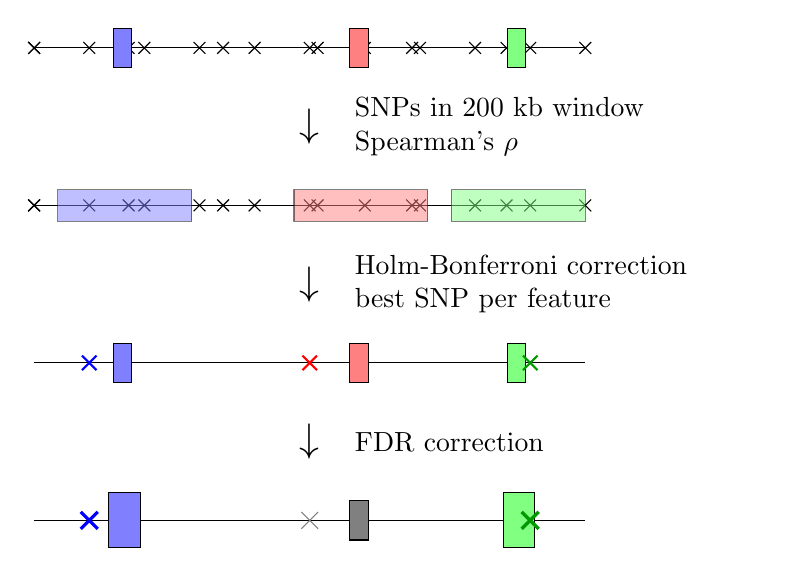
\begin{tikzpicture}
    [feature/.style={rectangle, draw, minimum height=5mm},
     cross/.style={cross out, draw, minimum size=2*(#1-\pgflinewidth), 
     inner sep=0pt, outer sep=0pt},
     cross/.default={1.2mm}]
    \coordinate (5prime);
    \coordinate [right=7cm of 5prime] (3prime);
    \draw (5prime) -- (3prime);
    \draw [decorate, decoration={crosses, segment length=7mm, shape size=1.5mm}]
          (5prime) -- (3prime);
    \draw [decorate, 
           decoration={crosses, segment length=12mm, shape size=1.5mm}] 
          (5prime) -- (3prime);
    \node [feature, right=1cm of 5prime, fill=blue!50!white] (f1) { };
    \node [feature, right=4cm of 5prime, fill=red!50!white] (f2) { };
    \node [feature, right=6cm of 5prime, fill=green!50!white] (f3) { };

    \uncover<2->{

    \coordinate [below=2cm of 5prime] (5prime2);
    \coordinate [below=2cm of 3prime] (3prime2);
    \draw (5prime2) -- (3prime2);
    \draw [decorate, decoration={crosses, segment length=7mm, shape size=1.5mm}]
          (5prime2) -- (3prime2);
    \draw [decorate, 
           decoration={crosses, segment length=12mm, shape size=1.5mm}] 
          (5prime2) -- (3prime2);
    \draw [fill=blue!50!white, opacity=0.5] ($(5prime2) + (0.3cm, 0.2cm)$) 
          rectangle ($(5prime2) + (2cm, -0.2cm)$);
    \draw [fill=red!50!white, opacity=0.5] ($(5prime2) + (3.3cm, 0.2cm)$) 
          rectangle ($(5prime2) + (5cm, -0.2cm)$);
    \draw [fill=green!50!white, opacity=0.5] ($(5prime2) + (5.3cm, 0.2cm)$) 
          rectangle ($(5prime2) + (7cm, -0.2cm)$);
    \path (5prime) -- node (mid1) {\Large{$\downarrow$}} (3prime2);
    \node [right=2mm of mid1, text width=5cm] {SNPs in 200 kb window \\
    Spearman's $\rho$};

    }\uncover<3->{

    \coordinate [below=2cm of 5prime2] (5prime3);
    \coordinate [below=2cm of 3prime2] (3prime3);
    \draw (5prime3) -- (3prime3);
    \node [feature, right=1cm of 5prime3, fill=blue!50!white] (f1) { };
    \node [feature, right=4cm of 5prime3, fill=red!50!white] (f2) { };
    \node [feature, right=6cm of 5prime3, fill=green!50!white] (f3) { };
    \node [cross, blue, thick] at ($(5prime3) + (7mm, 0mm)$) { };
    \node [cross, red, thick] at ($(5prime3) + (35mm, 0mm)$) { };
    \node [cross, green!60!black, thick] at ($(5prime3) + (63mm, 0mm)$) { };
    \path (5prime2) -- node (mid2) {\Large{$\downarrow$}} (3prime3);
    \node [right=2mm of mid2, text width=5cm] {Holm-Bonferroni correction \\ best SNP per feature};

    }\uncover<4->{

    \coordinate [below=2cm of 5prime3] (5prime4);
    \coordinate [below=2cm of 3prime3] (3prime4);
    \draw (5prime4) -- (3prime4);
    \node [feature, minimum height=7mm, minimum width=4mm, right=1.15cm of
    5prime4, anchor=center, fill=blue!50!white] (f1) { };
    \node [feature, right=4cm of 5prime4, fill=gray] (f2) { };
    \node [feature, right=5.95cm of 5prime4, minimum height=7mm, minimum width=4mm, fill=green!50!white] (f3) { };
    \node [cross, cross=1.5mm, blue, very thick] at ($(5prime4) + (7mm, 0mm)$) { };
    \node [cross, gray] at ($(5prime4) + (35mm, 0mm)$) { };
    \node [cross, cross=1.5mm, green!60!black, very thick] at ($(5prime4) + (63mm, 0mm)$) { };
    \path (5prime3) -- node (mid3) {\Large{$\downarrow$}} (3prime4);
    \node [right=2mm of mid3] {FDR correction};

    }
\end{tikzpicture}

        \tikzexternalenable
    \end{center}
\end{frame}

\begin{frame}{Removing Principal Components}
    \begin{columns}
    \begin{column}{0.4\textwidth}
        \begin{itemize}
            \item technical, environmental, and biological covariates can swamp
                out QTL effects
            \uncover<2->{
            \item correct by removing principal components 
            }\uncover<3->{
            \item number of peaks with a QTL plateaus at 10 PCs, while genes and
                CpGs continue to increase
            }\uncover<4->{
            \item for this analysis, removed 10 PCs from all data
            }
        \end{itemize}
    \end{column}
    \begin{column}{0.6\textwidth}
        % Created by tikzDevice version 0.7.0 on 2015-04-17 14:29:37
% !TEX encoding = UTF-8 Unicode
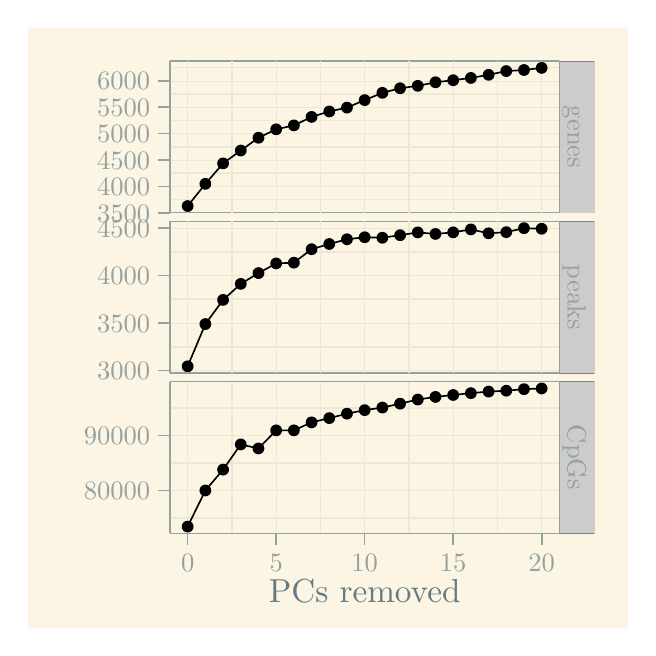
\begin{tikzpicture}[x=1pt,y=1pt]
\definecolor[named]{fillColor}{rgb}{0.99,0.96,0.89}
\path[use as bounding box,fill=fillColor] (0,0) rectangle (216.81,216.81);
\begin{scope}
\path[clip] (  0.00,  0.00) rectangle (216.81,216.81);

\path[fill=fillColor] (  0.00,  0.00) rectangle (216.81,216.81);
\end{scope}
\begin{scope}
\path[clip] ( 51.42,149.86) rectangle (192.13,204.77);
\definecolor[named]{drawColor}{rgb}{0.58,0.63,0.63}
\definecolor[named]{fillColor}{rgb}{0.99,0.96,0.89}

\path[draw=drawColor,line width= 0.6pt,line join=round,line cap=round,fill=fillColor] ( 51.42,149.86) rectangle (192.13,204.77);
\definecolor[named]{drawColor}{rgb}{0.93,0.91,0.84}

\path[draw=drawColor,line width= 0.6pt,line join=round] ( 51.42,154.67) --
	(192.13,154.67);

\path[draw=drawColor,line width= 0.6pt,line join=round] ( 51.42,164.21) --
	(192.13,164.21);

\path[draw=drawColor,line width= 0.6pt,line join=round] ( 51.42,173.75) --
	(192.13,173.75);

\path[draw=drawColor,line width= 0.6pt,line join=round] ( 51.42,183.29) --
	(192.13,183.29);

\path[draw=drawColor,line width= 0.6pt,line join=round] ( 51.42,192.83) --
	(192.13,192.83);

\path[draw=drawColor,line width= 0.6pt,line join=round] ( 51.42,202.36) --
	(192.13,202.36);

\path[draw=drawColor,line width= 0.6pt,line join=round] ( 73.80,149.86) --
	( 73.80,204.77);

\path[draw=drawColor,line width= 0.6pt,line join=round] (105.78,149.86) --
	(105.78,204.77);

\path[draw=drawColor,line width= 0.6pt,line join=round] (137.76,149.86) --
	(137.76,204.77);

\path[draw=drawColor,line width= 0.6pt,line join=round] (169.74,149.86) --
	(169.74,204.77);

\path[draw=drawColor,line width= 0.2pt,line join=round] ( 51.42,149.90) --
	(192.13,149.90);

\path[draw=drawColor,line width= 0.2pt,line join=round] ( 51.42,159.44) --
	(192.13,159.44);

\path[draw=drawColor,line width= 0.2pt,line join=round] ( 51.42,168.98) --
	(192.13,168.98);

\path[draw=drawColor,line width= 0.2pt,line join=round] ( 51.42,178.52) --
	(192.13,178.52);

\path[draw=drawColor,line width= 0.2pt,line join=round] ( 51.42,188.06) --
	(192.13,188.06);

\path[draw=drawColor,line width= 0.2pt,line join=round] ( 51.42,197.59) --
	(192.13,197.59);

\path[draw=drawColor,line width= 0.2pt,line join=round] ( 57.81,149.86) --
	( 57.81,204.77);

\path[draw=drawColor,line width= 0.2pt,line join=round] ( 89.79,149.86) --
	( 89.79,204.77);

\path[draw=drawColor,line width= 0.2pt,line join=round] (121.77,149.86) --
	(121.77,204.77);

\path[draw=drawColor,line width= 0.2pt,line join=round] (153.75,149.86) --
	(153.75,204.77);

\path[draw=drawColor,line width= 0.2pt,line join=round] (185.73,149.86) --
	(185.73,204.77);
\definecolor[named]{fillColor}{rgb}{0.00,0.00,0.00}

\path[fill=fillColor] ( 57.81,152.36) circle (  2.13);

\path[fill=fillColor] ( 64.21,160.37) circle (  2.13);

\path[fill=fillColor] ( 70.61,167.77) circle (  2.13);

\path[fill=fillColor] ( 77.00,172.41) circle (  2.13);

\path[fill=fillColor] ( 83.40,177.03) circle (  2.13);

\path[fill=fillColor] ( 89.79,180.08) circle (  2.13);

\path[fill=fillColor] ( 96.19,181.49) circle (  2.13);

\path[fill=fillColor] (102.59,184.56) circle (  2.13);

\path[fill=fillColor] (108.98,186.53) circle (  2.13);

\path[fill=fillColor] (115.38,187.92) circle (  2.13);

\path[fill=fillColor] (121.77,190.63) circle (  2.13);

\path[fill=fillColor] (128.17,193.26) circle (  2.13);

\path[fill=fillColor] (134.57,194.92) circle (  2.13);

\path[fill=fillColor] (140.96,195.80) circle (  2.13);

\path[fill=fillColor] (147.36,197.08) circle (  2.13);

\path[fill=fillColor] (153.75,197.82) circle (  2.13);

\path[fill=fillColor] (160.15,198.64) circle (  2.13);

\path[fill=fillColor] (166.55,199.77) circle (  2.13);

\path[fill=fillColor] (172.94,201.12) circle (  2.13);

\path[fill=fillColor] (179.34,201.51) circle (  2.13);

\path[fill=fillColor] (185.73,202.27) circle (  2.13);
\definecolor[named]{drawColor}{rgb}{0.00,0.00,0.00}

\path[draw=drawColor,line width= 0.6pt,line join=round] ( 57.81,152.36) --
	( 64.21,160.37) --
	( 70.61,167.77) --
	( 77.00,172.41) --
	( 83.40,177.03) --
	( 89.79,180.08) --
	( 96.19,181.49) --
	(102.59,184.56) --
	(108.98,186.53) --
	(115.38,187.92) --
	(121.77,190.63) --
	(128.17,193.26) --
	(134.57,194.92) --
	(140.96,195.80) --
	(147.36,197.08) --
	(153.75,197.82) --
	(160.15,198.64) --
	(166.55,199.77) --
	(172.94,201.12) --
	(179.34,201.51) --
	(185.73,202.27);
\end{scope}
\begin{scope}
\path[clip] ( 51.42, 91.95) rectangle (192.13,146.85);
\definecolor[named]{drawColor}{rgb}{0.58,0.63,0.63}
\definecolor[named]{fillColor}{rgb}{0.99,0.96,0.89}

\path[draw=drawColor,line width= 0.6pt,line join=round,line cap=round,fill=fillColor] ( 51.42, 91.95) rectangle (192.13,146.85);
\definecolor[named]{drawColor}{rgb}{0.93,0.91,0.84}

\path[draw=drawColor,line width= 0.6pt,line join=round] ( 51.42,101.53) --
	(192.13,101.53);

\path[draw=drawColor,line width= 0.6pt,line join=round] ( 51.42,118.65) --
	(192.13,118.65);

\path[draw=drawColor,line width= 0.6pt,line join=round] ( 51.42,135.76) --
	(192.13,135.76);

\path[draw=drawColor,line width= 0.6pt,line join=round] ( 73.80, 91.95) --
	( 73.80,146.85);

\path[draw=drawColor,line width= 0.6pt,line join=round] (105.78, 91.95) --
	(105.78,146.85);

\path[draw=drawColor,line width= 0.6pt,line join=round] (137.76, 91.95) --
	(137.76,146.85);

\path[draw=drawColor,line width= 0.6pt,line join=round] (169.74, 91.95) --
	(169.74,146.85);

\path[draw=drawColor,line width= 0.2pt,line join=round] ( 51.42, 92.97) --
	(192.13, 92.97);

\path[draw=drawColor,line width= 0.2pt,line join=round] ( 51.42,110.09) --
	(192.13,110.09);

\path[draw=drawColor,line width= 0.2pt,line join=round] ( 51.42,127.20) --
	(192.13,127.20);

\path[draw=drawColor,line width= 0.2pt,line join=round] ( 51.42,144.32) --
	(192.13,144.32);

\path[draw=drawColor,line width= 0.2pt,line join=round] ( 57.81, 91.95) --
	( 57.81,146.85);

\path[draw=drawColor,line width= 0.2pt,line join=round] ( 89.79, 91.95) --
	( 89.79,146.85);

\path[draw=drawColor,line width= 0.2pt,line join=round] (121.77, 91.95) --
	(121.77,146.85);

\path[draw=drawColor,line width= 0.2pt,line join=round] (153.75, 91.95) --
	(153.75,146.85);

\path[draw=drawColor,line width= 0.2pt,line join=round] (185.73, 91.95) --
	(185.73,146.85);
\definecolor[named]{fillColor}{rgb}{0.00,0.00,0.00}

\path[fill=fillColor] ( 57.81, 94.44) circle (  2.13);

\path[fill=fillColor] ( 64.21,109.71) circle (  2.13);

\path[fill=fillColor] ( 70.61,118.44) circle (  2.13);

\path[fill=fillColor] ( 77.00,124.23) circle (  2.13);

\path[fill=fillColor] ( 83.40,128.13) circle (  2.13);

\path[fill=fillColor] ( 89.79,131.62) circle (  2.13);

\path[fill=fillColor] ( 96.19,131.89) circle (  2.13);

\path[fill=fillColor] (102.59,136.76) circle (  2.13);

\path[fill=fillColor] (108.98,138.64) circle (  2.13);

\path[fill=fillColor] (115.38,140.35) circle (  2.13);

\path[fill=fillColor] (121.77,141.07) circle (  2.13);

\path[fill=fillColor] (128.17,140.90) circle (  2.13);

\path[fill=fillColor] (134.57,141.82) circle (  2.13);

\path[fill=fillColor] (140.96,142.82) circle (  2.13);

\path[fill=fillColor] (147.36,142.27) circle (  2.13);

\path[fill=fillColor] (153.75,142.85) circle (  2.13);

\path[fill=fillColor] (160.15,143.91) circle (  2.13);

\path[fill=fillColor] (166.55,142.51) circle (  2.13);

\path[fill=fillColor] (172.94,142.92) circle (  2.13);

\path[fill=fillColor] (179.34,144.36) circle (  2.13);

\path[fill=fillColor] (185.73,144.15) circle (  2.13);
\definecolor[named]{drawColor}{rgb}{0.00,0.00,0.00}

\path[draw=drawColor,line width= 0.6pt,line join=round] ( 57.81, 94.44) --
	( 64.21,109.71) --
	( 70.61,118.44) --
	( 77.00,124.23) --
	( 83.40,128.13) --
	( 89.79,131.62) --
	( 96.19,131.89) --
	(102.59,136.76) --
	(108.98,138.64) --
	(115.38,140.35) --
	(121.77,141.07) --
	(128.17,140.90) --
	(134.57,141.82) --
	(140.96,142.82) --
	(147.36,142.27) --
	(153.75,142.85) --
	(160.15,143.91) --
	(166.55,142.51) --
	(172.94,142.92) --
	(179.34,144.36) --
	(185.73,144.15);
\end{scope}
\begin{scope}
\path[clip] ( 51.42, 34.03) rectangle (192.13, 88.94);
\definecolor[named]{drawColor}{rgb}{0.58,0.63,0.63}
\definecolor[named]{fillColor}{rgb}{0.99,0.96,0.89}

\path[draw=drawColor,line width= 0.6pt,line join=round,line cap=round,fill=fillColor] ( 51.42, 34.03) rectangle (192.13, 88.94);
\definecolor[named]{drawColor}{rgb}{0.93,0.91,0.84}

\path[draw=drawColor,line width= 0.6pt,line join=round] ( 51.42, 39.69) --
	(192.13, 39.69);

\path[draw=drawColor,line width= 0.6pt,line join=round] ( 51.42, 59.50) --
	(192.13, 59.50);

\path[draw=drawColor,line width= 0.6pt,line join=round] ( 51.42, 79.32) --
	(192.13, 79.32);

\path[draw=drawColor,line width= 0.6pt,line join=round] ( 73.80, 34.03) --
	( 73.80, 88.94);

\path[draw=drawColor,line width= 0.6pt,line join=round] (105.78, 34.03) --
	(105.78, 88.94);

\path[draw=drawColor,line width= 0.6pt,line join=round] (137.76, 34.03) --
	(137.76, 88.94);

\path[draw=drawColor,line width= 0.6pt,line join=round] (169.74, 34.03) --
	(169.74, 88.94);

\path[draw=drawColor,line width= 0.2pt,line join=round] ( 51.42, 49.60) --
	(192.13, 49.60);

\path[draw=drawColor,line width= 0.2pt,line join=round] ( 51.42, 69.41) --
	(192.13, 69.41);

\path[draw=drawColor,line width= 0.2pt,line join=round] ( 57.81, 34.03) --
	( 57.81, 88.94);

\path[draw=drawColor,line width= 0.2pt,line join=round] ( 89.79, 34.03) --
	( 89.79, 88.94);

\path[draw=drawColor,line width= 0.2pt,line join=round] (121.77, 34.03) --
	(121.77, 88.94);

\path[draw=drawColor,line width= 0.2pt,line join=round] (153.75, 34.03) --
	(153.75, 88.94);

\path[draw=drawColor,line width= 0.2pt,line join=round] (185.73, 34.03) --
	(185.73, 88.94);
\definecolor[named]{fillColor}{rgb}{0.00,0.00,0.00}

\path[fill=fillColor] ( 57.81, 36.53) circle (  2.13);

\path[fill=fillColor] ( 64.21, 49.57) circle (  2.13);

\path[fill=fillColor] ( 70.61, 57.11) circle (  2.13);

\path[fill=fillColor] ( 77.00, 66.22) circle (  2.13);

\path[fill=fillColor] ( 83.40, 64.76) circle (  2.13);

\path[fill=fillColor] ( 89.79, 71.30) circle (  2.13);

\path[fill=fillColor] ( 96.19, 71.31) circle (  2.13);

\path[fill=fillColor] (102.59, 74.18) circle (  2.13);

\path[fill=fillColor] (108.98, 75.72) circle (  2.13);

\path[fill=fillColor] (115.38, 77.32) circle (  2.13);

\path[fill=fillColor] (121.77, 78.60) circle (  2.13);

\path[fill=fillColor] (128.17, 79.54) circle (  2.13);

\path[fill=fillColor] (134.57, 80.94) circle (  2.13);

\path[fill=fillColor] (140.96, 82.43) circle (  2.13);

\path[fill=fillColor] (147.36, 83.38) circle (  2.13);

\path[fill=fillColor] (153.75, 84.08) circle (  2.13);

\path[fill=fillColor] (160.15, 84.75) circle (  2.13);

\path[fill=fillColor] (166.55, 85.31) circle (  2.13);

\path[fill=fillColor] (172.94, 85.63) circle (  2.13);

\path[fill=fillColor] (179.34, 86.18) circle (  2.13);

\path[fill=fillColor] (185.73, 86.44) circle (  2.13);
\definecolor[named]{drawColor}{rgb}{0.00,0.00,0.00}

\path[draw=drawColor,line width= 0.6pt,line join=round] ( 57.81, 36.53) --
	( 64.21, 49.57) --
	( 70.61, 57.11) --
	( 77.00, 66.22) --
	( 83.40, 64.76) --
	( 89.79, 71.30) --
	( 96.19, 71.31) --
	(102.59, 74.18) --
	(108.98, 75.72) --
	(115.38, 77.32) --
	(121.77, 78.60) --
	(128.17, 79.54) --
	(134.57, 80.94) --
	(140.96, 82.43) --
	(147.36, 83.38) --
	(153.75, 84.08) --
	(160.15, 84.75) --
	(166.55, 85.31) --
	(172.94, 85.63) --
	(179.34, 86.18) --
	(185.73, 86.44);
\end{scope}
\begin{scope}
\path[clip] (  0.00,  0.00) rectangle (216.81,216.81);
\definecolor[named]{drawColor}{rgb}{0.58,0.63,0.63}

\path[draw=drawColor,line width= 0.6pt,line join=round] ( 51.42,149.86) --
	( 51.42,204.77);
\end{scope}
\begin{scope}
\path[clip] (  0.00,  0.00) rectangle (216.81,216.81);
\definecolor[named]{drawColor}{rgb}{0.58,0.63,0.63}

\node[text=drawColor,anchor=base east,inner sep=0pt, outer sep=0pt, scale=  0.96] at ( 44.30,146.59) {3500};

\node[text=drawColor,anchor=base east,inner sep=0pt, outer sep=0pt, scale=  0.96] at ( 44.30,156.13) {4000};

\node[text=drawColor,anchor=base east,inner sep=0pt, outer sep=0pt, scale=  0.96] at ( 44.30,165.67) {4500};

\node[text=drawColor,anchor=base east,inner sep=0pt, outer sep=0pt, scale=  0.96] at ( 44.30,175.21) {5000};

\node[text=drawColor,anchor=base east,inner sep=0pt, outer sep=0pt, scale=  0.96] at ( 44.30,184.75) {5500};

\node[text=drawColor,anchor=base east,inner sep=0pt, outer sep=0pt, scale=  0.96] at ( 44.30,194.29) {6000};
\end{scope}
\begin{scope}
\path[clip] (  0.00,  0.00) rectangle (216.81,216.81);
\definecolor[named]{drawColor}{rgb}{0.58,0.63,0.63}

\path[draw=drawColor,line width= 0.6pt,line join=round] ( 47.15,149.90) --
	( 51.42,149.90);

\path[draw=drawColor,line width= 0.6pt,line join=round] ( 47.15,159.44) --
	( 51.42,159.44);

\path[draw=drawColor,line width= 0.6pt,line join=round] ( 47.15,168.98) --
	( 51.42,168.98);

\path[draw=drawColor,line width= 0.6pt,line join=round] ( 47.15,178.52) --
	( 51.42,178.52);

\path[draw=drawColor,line width= 0.6pt,line join=round] ( 47.15,188.06) --
	( 51.42,188.06);

\path[draw=drawColor,line width= 0.6pt,line join=round] ( 47.15,197.59) --
	( 51.42,197.59);
\end{scope}
\begin{scope}
\path[clip] (  0.00,  0.00) rectangle (216.81,216.81);
\definecolor[named]{drawColor}{rgb}{0.58,0.63,0.63}

\path[draw=drawColor,line width= 0.6pt,line join=round] ( 51.42, 91.95) --
	( 51.42,146.85);
\end{scope}
\begin{scope}
\path[clip] (  0.00,  0.00) rectangle (216.81,216.81);
\definecolor[named]{drawColor}{rgb}{0.58,0.63,0.63}

\node[text=drawColor,anchor=base east,inner sep=0pt, outer sep=0pt, scale=  0.96] at ( 44.30, 89.67) {3000};

\node[text=drawColor,anchor=base east,inner sep=0pt, outer sep=0pt, scale=  0.96] at ( 44.30,106.78) {3500};

\node[text=drawColor,anchor=base east,inner sep=0pt, outer sep=0pt, scale=  0.96] at ( 44.30,123.90) {4000};

\node[text=drawColor,anchor=base east,inner sep=0pt, outer sep=0pt, scale=  0.96] at ( 44.30,141.02) {4500};
\end{scope}
\begin{scope}
\path[clip] (  0.00,  0.00) rectangle (216.81,216.81);
\definecolor[named]{drawColor}{rgb}{0.58,0.63,0.63}

\path[draw=drawColor,line width= 0.6pt,line join=round] ( 47.15, 92.97) --
	( 51.42, 92.97);

\path[draw=drawColor,line width= 0.6pt,line join=round] ( 47.15,110.09) --
	( 51.42,110.09);

\path[draw=drawColor,line width= 0.6pt,line join=round] ( 47.15,127.20) --
	( 51.42,127.20);

\path[draw=drawColor,line width= 0.6pt,line join=round] ( 47.15,144.32) --
	( 51.42,144.32);
\end{scope}
\begin{scope}
\path[clip] (  0.00,  0.00) rectangle (216.81,216.81);
\definecolor[named]{drawColor}{rgb}{0.58,0.63,0.63}

\path[draw=drawColor,line width= 0.6pt,line join=round] ( 51.42, 34.03) --
	( 51.42, 88.94);
\end{scope}
\begin{scope}
\path[clip] (  0.00,  0.00) rectangle (216.81,216.81);
\definecolor[named]{drawColor}{rgb}{0.58,0.63,0.63}

\node[text=drawColor,anchor=base east,inner sep=0pt, outer sep=0pt, scale=  0.96] at ( 44.30, 46.29) {80000};

\node[text=drawColor,anchor=base east,inner sep=0pt, outer sep=0pt, scale=  0.96] at ( 44.30, 66.11) {90000};
\end{scope}
\begin{scope}
\path[clip] (  0.00,  0.00) rectangle (216.81,216.81);
\definecolor[named]{drawColor}{rgb}{0.58,0.63,0.63}

\path[draw=drawColor,line width= 0.6pt,line join=round] ( 47.15, 49.60) --
	( 51.42, 49.60);

\path[draw=drawColor,line width= 0.6pt,line join=round] ( 47.15, 69.41) --
	( 51.42, 69.41);
\end{scope}
\begin{scope}
\path[clip] (192.13,149.86) rectangle (204.76,204.77);
\definecolor[named]{drawColor}{rgb}{0.50,0.50,0.50}
\definecolor[named]{fillColor}{rgb}{0.80,0.80,0.80}

\path[draw=drawColor,line width= 0.2pt,line join=round,line cap=round,fill=fillColor] (192.13,149.86) rectangle (204.76,204.77);
\definecolor[named]{drawColor}{rgb}{0.58,0.63,0.63}

\node[text=drawColor,rotate=270.00,anchor=base,inner sep=0pt, outer sep=0pt, scale=  0.96] at (195.14,177.31) {genes};
\end{scope}
\begin{scope}
\path[clip] (192.13, 91.95) rectangle (204.76,146.85);
\definecolor[named]{drawColor}{rgb}{0.50,0.50,0.50}
\definecolor[named]{fillColor}{rgb}{0.80,0.80,0.80}

\path[draw=drawColor,line width= 0.2pt,line join=round,line cap=round,fill=fillColor] (192.13, 91.95) rectangle (204.76,146.85);
\definecolor[named]{drawColor}{rgb}{0.58,0.63,0.63}

\node[text=drawColor,rotate=270.00,anchor=base,inner sep=0pt, outer sep=0pt, scale=  0.96] at (195.14,119.40) {peaks};
\end{scope}
\begin{scope}
\path[clip] (192.13, 34.03) rectangle (204.76, 88.94);
\definecolor[named]{drawColor}{rgb}{0.50,0.50,0.50}
\definecolor[named]{fillColor}{rgb}{0.80,0.80,0.80}

\path[draw=drawColor,line width= 0.2pt,line join=round,line cap=round,fill=fillColor] (192.13, 34.03) rectangle (204.76, 88.94);
\definecolor[named]{drawColor}{rgb}{0.58,0.63,0.63}

\node[text=drawColor,rotate=270.00,anchor=base,inner sep=0pt, outer sep=0pt, scale=  0.96] at (195.14, 61.49) {CpGs};
\end{scope}
\begin{scope}
\path[clip] (  0.00,  0.00) rectangle (216.81,216.81);
\definecolor[named]{drawColor}{rgb}{0.58,0.63,0.63}

\path[draw=drawColor,line width= 0.6pt,line join=round] ( 51.42, 34.03) --
	(192.13, 34.03);
\end{scope}
\begin{scope}
\path[clip] (  0.00,  0.00) rectangle (216.81,216.81);
\definecolor[named]{drawColor}{rgb}{0.58,0.63,0.63}

\path[draw=drawColor,line width= 0.6pt,line join=round] ( 57.81, 29.77) --
	( 57.81, 34.03);

\path[draw=drawColor,line width= 0.6pt,line join=round] ( 89.79, 29.77) --
	( 89.79, 34.03);

\path[draw=drawColor,line width= 0.6pt,line join=round] (121.77, 29.77) --
	(121.77, 34.03);

\path[draw=drawColor,line width= 0.6pt,line join=round] (153.75, 29.77) --
	(153.75, 34.03);

\path[draw=drawColor,line width= 0.6pt,line join=round] (185.73, 29.77) --
	(185.73, 34.03);
\end{scope}
\begin{scope}
\path[clip] (  0.00,  0.00) rectangle (216.81,216.81);
\definecolor[named]{drawColor}{rgb}{0.58,0.63,0.63}

\node[text=drawColor,anchor=base,inner sep=0pt, outer sep=0pt, scale=  0.96] at ( 57.81, 20.31) {0};

\node[text=drawColor,anchor=base,inner sep=0pt, outer sep=0pt, scale=  0.96] at ( 89.79, 20.31) {5};

\node[text=drawColor,anchor=base,inner sep=0pt, outer sep=0pt, scale=  0.96] at (121.77, 20.31) {10};

\node[text=drawColor,anchor=base,inner sep=0pt, outer sep=0pt, scale=  0.96] at (153.75, 20.31) {15};

\node[text=drawColor,anchor=base,inner sep=0pt, outer sep=0pt, scale=  0.96] at (185.73, 20.31) {20};
\end{scope}
\begin{scope}
\path[clip] (  0.00,  0.00) rectangle (216.81,216.81);
\definecolor[named]{drawColor}{rgb}{0.40,0.48,0.51}

\node[text=drawColor,anchor=base,inner sep=0pt, outer sep=0pt, scale=  1.20] at (121.77,  9.03) {PCs removed};
\end{scope}
\end{tikzpicture}

    \end{column}
    \end{columns}
\end{frame}

\begin{frame}{Identifying multi-QTLs}
\begin{columns}
    \begin{column}{0.5\textwidth}
        \begin{itemize}
            \item By intersecting QTL sets, found 240 gene, CpG, and peak
                triples which shared the same QTL 
        \end{itemize}
        % Created by tikzDevice version 0.7.0 on 2015-04-17 18:24:44
% !TEX encoding = UTF-8 Unicode
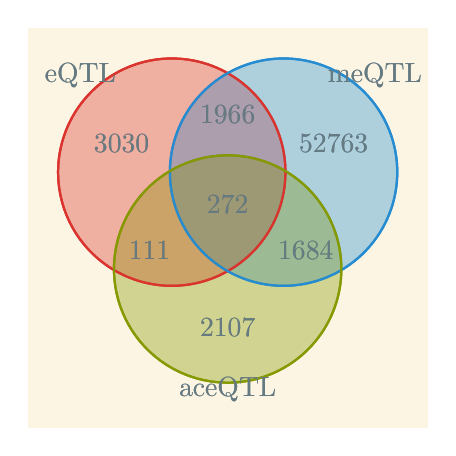
\begin{tikzpicture}[x=1pt,y=1pt]
\definecolor[named]{fillColor}{rgb}{0.99,0.96,0.89}
\path[use as bounding box,fill=fillColor] (0,0) rectangle (144.54,144.54);
\begin{scope}
\path[clip] (  0.00,  0.00) rectangle (144.54,144.54);
\definecolor[named]{fillColor}{rgb}{0.86,0.20,0.18}

\path[fill=fillColor,fill opacity=0.20] ( 93.14, 92.33) --
	( 93.14, 92.42) --
	( 93.14, 92.51) --
	( 93.14, 92.59) --
	( 93.14, 92.68) --
	( 93.14, 92.76) --
	( 93.14, 92.85) --
	( 93.14, 92.94) --
	( 93.14, 93.02) --
	( 93.13, 93.11) --
	( 93.13, 93.19) --
	( 93.13, 93.28) --
	( 93.13, 93.37) --
	( 93.13, 93.45) --
	( 93.12, 93.54) --
	( 93.12, 93.62) --
	( 93.12, 93.71) --
	( 93.12, 93.80) --
	( 93.11, 93.88) --
	( 93.11, 93.97) --
	( 93.11, 94.05) --
	( 93.10, 94.14) --
	( 93.10, 94.23) --
	( 93.09, 94.31) --
	( 93.09, 94.40) --
	( 93.09, 94.48) --
	( 93.08, 94.57) --
	( 93.08, 94.66) --
	( 93.07, 94.74) --
	( 93.07, 94.83) --
	( 93.06, 94.91) --
	( 93.06, 95.00) --
	( 93.05, 95.08) --
	( 93.04, 95.17) --
	( 93.04, 95.26) --
	( 93.03, 95.34) --
	( 93.03, 95.43) --
	( 93.02, 95.51) --
	( 93.01, 95.60) --
	( 93.01, 95.69) --
	( 93.00, 95.77) --
	( 92.99, 95.86) --
	( 92.98, 95.94) --
	( 92.98, 96.03) --
	( 92.97, 96.11) --
	( 92.96, 96.20) --
	( 92.95, 96.28) --
	( 92.94, 96.37) --
	( 92.93, 96.46) --
	( 92.93, 96.54) --
	( 92.92, 96.63) --
	( 92.91, 96.71) --
	( 92.90, 96.80) --
	( 92.89, 96.88) --
	( 92.88, 96.97) --
	( 92.87, 97.05) --
	( 92.86, 97.14) --
	( 92.85, 97.23) --
	( 92.84, 97.31) --
	( 92.83, 97.40) --
	( 92.82, 97.48) --
	( 92.81, 97.57) --
	( 92.80, 97.65) --
	( 92.79, 97.74) --
	( 92.77, 97.82) --
	( 92.76, 97.91) --
	( 92.75, 97.99) --
	( 92.74, 98.08) --
	( 92.73, 98.16) --
	( 92.71, 98.25) --
	( 92.70, 98.33) --
	( 92.69, 98.42) --
	( 92.68, 98.50) --
	( 92.66, 98.59) --
	( 92.65, 98.67) --
	( 92.64, 98.76) --
	( 92.62, 98.84) --
	( 92.61, 98.93) --
	( 92.60, 99.01) --
	( 92.58, 99.10) --
	( 92.57, 99.18) --
	( 92.55, 99.27) --
	( 92.54, 99.35) --
	( 92.52, 99.44) --
	( 92.51, 99.52) --
	( 92.49, 99.61) --
	( 92.48, 99.69) --
	( 92.46, 99.78) --
	( 92.45, 99.86) --
	( 92.43, 99.95) --
	( 92.41,100.03) --
	( 92.40,100.11) --
	( 92.38,100.20) --
	( 92.37,100.28) --
	( 92.35,100.37) --
	( 92.33,100.45) --
	( 92.31,100.54) --
	( 92.30,100.62) --
	( 92.28,100.71) --
	( 92.26,100.79) --
	( 92.24,100.87) --
	( 92.23,100.96) --
	( 92.21,101.04) --
	( 92.19,101.13) --
	( 92.17,101.21) --
	( 92.15,101.29) --
	( 92.13,101.38) --
	( 92.12,101.46) --
	( 92.10,101.55) --
	( 92.08,101.63) --
	( 92.06,101.71) --
	( 92.04,101.80) --
	( 92.02,101.88) --
	( 92.00,101.96) --
	( 91.98,102.05) --
	( 91.96,102.13) --
	( 91.94,102.22) --
	( 91.92,102.30) --
	( 91.89,102.38) --
	( 91.87,102.47) --
	( 91.85,102.55) --
	( 91.83,102.63) --
	( 91.81,102.72) --
	( 91.79,102.80) --
	( 91.76,102.88) --
	( 91.74,102.96) --
	( 91.72,103.05) --
	( 91.70,103.13) --
	( 91.67,103.21) --
	( 91.65,103.30) --
	( 91.63,103.38) --
	( 91.61,103.46) --
	( 91.58,103.55) --
	( 91.56,103.63) --
	( 91.54,103.71) --
	( 91.51,103.79) --
	( 91.49,103.88) --
	( 91.46,103.96) --
	( 91.44,104.04) --
	( 91.41,104.12) --
	( 91.39,104.21) --
	( 91.36,104.29) --
	( 91.34,104.37) --
	( 91.31,104.45) --
	( 91.29,104.53) --
	( 91.26,104.62) --
	( 91.24,104.70) --
	( 91.21,104.78) --
	( 91.18,104.86) --
	( 91.16,104.94) --
	( 91.13,105.03) --
	( 91.11,105.11) --
	( 91.08,105.19) --
	( 91.05,105.27) --
	( 91.02,105.35) --
	( 91.00,105.44) --
	( 90.97,105.52) --
	( 90.94,105.60) --
	( 90.91,105.68) --
	( 90.89,105.76) --
	( 90.86,105.84) --
	( 90.83,105.92) --
	( 90.80,106.00) --
	( 90.77,106.09) --
	( 90.74,106.17) --
	( 90.71,106.25) --
	( 90.68,106.33) --
	( 90.66,106.41) --
	( 90.63,106.49) --
	( 90.60,106.57) --
	( 90.57,106.65) --
	( 90.54,106.73) --
	( 90.51,106.81) --
	( 90.48,106.89) --
	( 90.44,106.97) --
	( 90.41,107.05) --
	( 90.38,107.13) --
	( 90.35,107.21) --
	( 90.32,107.29) --
	( 90.29,107.37) --
	( 90.26,107.45) --
	( 90.23,107.53) --
	( 90.19,107.61) --
	( 90.16,107.69) --
	( 90.13,107.77) --
	( 90.10,107.85) --
	( 90.06,107.93) --
	( 90.03,108.01) --
	( 90.00,108.09) --
	( 89.97,108.17) --
	( 89.93,108.25) --
	( 89.90,108.33) --
	( 89.87,108.41) --
	( 89.83,108.49) --
	( 89.80,108.57) --
	( 89.76,108.65) --
	( 89.73,108.73) --
	( 89.70,108.80) --
	( 89.66,108.88) --
	( 89.63,108.96) --
	( 89.59,109.04) --
	( 89.56,109.12) --
	( 89.52,109.20) --
	( 89.49,109.28) --
	( 89.45,109.35) --
	( 89.41,109.43) --
	( 89.38,109.51) --
	( 89.34,109.59) --
	( 89.31,109.67) --
	( 89.27,109.74) --
	( 89.23,109.82) --
	( 89.20,109.90) --
	( 89.16,109.98) --
	( 89.12,110.06) --
	( 89.09,110.13) --
	( 89.05,110.21) --
	( 89.01,110.29) --
	( 88.97,110.37) --
	( 88.93,110.44) --
	( 88.90,110.52) --
	( 88.86,110.60) --
	( 88.82,110.67) --
	( 88.78,110.75) --
	( 88.74,110.83) --
	( 88.70,110.90) --
	( 88.67,110.98) --
	( 88.63,111.06) --
	( 88.59,111.13) --
	( 88.55,111.21) --
	( 88.51,111.29) --
	( 88.47,111.36) --
	( 88.43,111.44) --
	( 88.39,111.52) --
	( 88.35,111.59) --
	( 88.31,111.67) --
	( 88.27,111.74) --
	( 88.23,111.82) --
	( 88.19,111.90) --
	( 88.14,111.97) --
	( 88.10,112.05) --
	( 88.06,112.12) --
	( 88.02,112.20) --
	( 87.98,112.27) --
	( 87.94,112.35) --
	( 87.89,112.42) --
	( 87.85,112.50) --
	( 87.81,112.57) --
	( 87.77,112.65) --
	( 87.72,112.72) --
	( 87.68,112.80) --
	( 87.64,112.87) --
	( 87.60,112.95) --
	( 87.55,113.02) --
	( 87.51,113.09) --
	( 87.47,113.17) --
	( 87.42,113.24) --
	( 87.38,113.32) --
	( 87.33,113.39) --
	( 87.29,113.46) --
	( 87.25,113.54) --
	( 87.20,113.61) --
	( 87.16,113.69) --
	( 87.11,113.76) --
	( 87.07,113.83) --
	( 87.02,113.91) --
	( 86.98,113.98) --
	( 86.93,114.05) --
	( 86.89,114.12) --
	( 86.84,114.20) --
	( 86.79,114.27) --
	( 86.75,114.34) --
	( 86.70,114.42) --
	( 86.66,114.49) --
	( 86.61,114.56) --
	( 86.56,114.63) --
	( 86.52,114.70) --
	( 86.47,114.78) --
	( 86.42,114.85) --
	( 86.37,114.92) --
	( 86.33,114.99) --
	( 86.28,115.06) --
	( 86.23,115.14) --
	( 86.18,115.21) --
	( 86.14,115.28) --
	( 86.09,115.35) --
	( 86.04,115.42) --
	( 85.99,115.49) --
	( 85.94,115.56) --
	( 85.89,115.63) --
	( 85.84,115.71) --
	( 85.80,115.78) --
	( 85.75,115.85) --
	( 85.70,115.92) --
	( 85.65,115.99) --
	( 85.60,116.06) --
	( 85.55,116.13) --
	( 85.50,116.20) --
	( 85.45,116.27) --
	( 85.40,116.34) --
	( 85.35,116.41) --
	( 85.30,116.48) --
	( 85.25,116.55) --
	( 85.20,116.62) --
	( 85.15,116.69) --
	( 85.09,116.75) --
	( 85.04,116.82) --
	( 84.99,116.89) --
	( 84.94,116.96) --
	( 84.89,117.03) --
	( 84.84,117.10) --
	( 84.78,117.17) --
	( 84.73,117.24) --
	( 84.68,117.30) --
	( 84.63,117.37) --
	( 84.58,117.44) --
	( 84.52,117.51) --
	( 84.47,117.58) --
	( 84.42,117.64) --
	( 84.36,117.71) --
	( 84.31,117.78) --
	( 84.26,117.85) --
	( 84.20,117.91) --
	( 84.15,117.98) --
	( 84.10,118.05) --
	( 84.04,118.12) --
	( 83.99,118.18) --
	( 83.93,118.25) --
	( 83.88,118.32) --
	( 83.83,118.38) --
	( 83.77,118.45) --
	( 83.72,118.52) --
	( 83.66,118.58) --
	( 83.61,118.65) --
	( 83.55,118.71) --
	( 83.50,118.78) --
	( 83.44,118.85) --
	( 83.38,118.91) --
	( 83.33,118.98) --
	( 83.27,119.04) --
	( 83.22,119.11) --
	( 83.16,119.17) --
	( 83.10,119.24) --
	( 83.05,119.30) --
	( 82.99,119.37) --
	( 82.93,119.43) --
	( 82.88,119.50) --
	( 82.82,119.56) --
	( 82.76,119.63) --
	( 82.71,119.69) --
	( 82.65,119.75) --
	( 82.59,119.82) --
	( 82.53,119.88) --
	( 82.48,119.95) --
	( 82.42,120.01) --
	( 82.36,120.07) --
	( 82.30,120.14) --
	( 82.24,120.20) --
	( 82.19,120.26) --
	( 82.13,120.33) --
	( 82.07,120.39) --
	( 82.01,120.45) --
	( 81.95,120.51) --
	( 81.89,120.58) --
	( 81.83,120.64) --
	( 81.77,120.70) --
	( 81.71,120.76) --
	( 81.65,120.83) --
	( 81.59,120.89) --
	( 81.53,120.95) --
	( 81.47,121.01) --
	( 81.41,121.07) --
	( 81.35,121.13) --
	( 81.29,121.20) --
	( 81.23,121.26) --
	( 81.17,121.32) --
	( 81.11,121.38) --
	( 81.05,121.44) --
	( 80.99,121.50) --
	( 80.93,121.56) --
	( 80.87,121.62) --
	( 80.81,121.68) --
	( 80.74,121.74) --
	( 80.68,121.80) --
	( 80.62,121.86) --
	( 80.56,121.92) --
	( 80.50,121.98) --
	( 80.43,122.04) --
	( 80.37,122.10) --
	( 80.31,122.16) --
	( 80.25,122.22) --
	( 80.18,122.28) --
	( 80.12,122.34) --
	( 80.06,122.39) --
	( 80.00,122.45) --
	( 79.93,122.51) --
	( 79.87,122.57) --
	( 79.81,122.63) --
	( 79.74,122.69) --
	( 79.68,122.74) --
	( 79.62,122.80) --
	( 79.55,122.86) --
	( 79.49,122.92) --
	( 79.42,122.97) --
	( 79.36,123.03) --
	( 79.29,123.09) --
	( 79.23,123.14) --
	( 79.17,123.20) --
	( 79.10,123.26) --
	( 79.04,123.31) --
	( 78.97,123.37) --
	( 78.91,123.43) --
	( 78.84,123.48) --
	( 78.78,123.54) --
	( 78.71,123.60) --
	( 78.64,123.65) --
	( 78.58,123.71) --
	( 78.51,123.76) --
	( 78.45,123.82) --
	( 78.38,123.87) --
	( 78.32,123.93) --
	( 78.25,123.98) --
	( 78.18,124.04) --
	( 78.12,124.09) --
	( 78.05,124.15) --
	( 77.98,124.20) --
	( 77.92,124.26) --
	( 77.85,124.31) --
	( 77.78,124.36) --
	( 77.72,124.42) --
	( 77.65,124.47) --
	( 77.58,124.52) --
	( 77.51,124.58) --
	( 77.45,124.63) --
	( 77.38,124.68) --
	( 77.31,124.74) --
	( 77.24,124.79) --
	( 77.17,124.84) --
	( 77.11,124.89) --
	( 77.04,124.95) --
	( 76.97,125.00) --
	( 76.90,125.05) --
	( 76.83,125.10) --
	( 76.76,125.16) --
	( 76.69,125.21) --
	( 76.63,125.26) --
	( 76.56,125.31) --
	( 76.49,125.36) --
	( 76.42,125.41) --
	( 76.35,125.46) --
	( 76.28,125.51) --
	( 76.21,125.56) --
	( 76.14,125.61) --
	( 76.07,125.67) --
	( 76.00,125.72) --
	( 75.93,125.77) --
	( 75.86,125.82) --
	( 75.79,125.87) --
	( 75.72,125.91) --
	( 75.65,125.96) --
	( 75.58,126.01) --
	( 75.51,126.06) --
	( 75.44,126.11) --
	( 75.37,126.16) --
	( 75.30,126.21) --
	( 75.23,126.26) --
	( 75.15,126.31) --
	( 75.08,126.35) --
	( 75.01,126.40) --
	( 74.94,126.45) --
	( 74.87,126.50) --
	( 74.80,126.55) --
	( 74.73,126.59) --
	( 74.65,126.64) --
	( 74.58,126.69) --
	( 74.51,126.74) --
	( 74.44,126.78) --
	( 74.37,126.83) --
	( 74.29,126.88) --
	( 74.22,126.92) --
	( 74.15,126.97) --
	( 74.08,127.01) --
	( 74.00,127.06) --
	( 73.93,127.11) --
	( 73.86,127.15) --
	( 73.78,127.20) --
	( 73.71,127.24) --
	( 73.64,127.29) --
	( 73.57,127.33) --
	( 73.49,127.38) --
	( 73.42,127.42) --
	( 73.34,127.47) --
	( 73.27,127.51) --
	( 73.20,127.56) --
	( 73.12,127.60) --
	( 73.05,127.65) --
	( 72.98,127.69) --
	( 72.90,127.73) --
	( 72.83,127.78) --
	( 72.75,127.82) --
	( 72.68,127.86) --
	( 72.60,127.91) --
	( 72.53,127.95) --
	( 72.46,127.99) --
	( 72.38,128.03) --
	( 72.31,128.08) --
	( 72.23,128.12) --
	( 72.16,128.16) --
	( 72.08,128.20) --
	( 72.01,128.25) --
	( 71.93,128.29) --
	( 71.86,128.33) --
	( 71.78,128.37) --
	( 71.70,128.41) --
	( 71.63,128.45) --
	( 71.55,128.49) --
	( 71.48,128.53) --
	( 71.40,128.57) --
	( 71.33,128.61) --
	( 71.25,128.65) --
	( 71.17,128.69) --
	( 71.10,128.73) --
	( 71.02,128.77) --
	( 70.94,128.81) --
	( 70.87,128.85) --
	( 70.79,128.89) --
	( 70.71,128.93) --
	( 70.64,128.97) --
	( 70.56,129.01) --
	( 70.48,129.05) --
	( 70.41,129.09) --
	( 70.33,129.13) --
	( 70.25,129.16) --
	( 70.18,129.20) --
	( 70.10,129.24) --
	( 70.02,129.28) --
	( 69.94,129.31) --
	( 69.87,129.35) --
	( 69.79,129.39) --
	( 69.71,129.43) --
	( 69.63,129.46) --
	( 69.56,129.50) --
	( 69.48,129.54) --
	( 69.40,129.57) --
	( 69.32,129.61) --
	( 69.24,129.64) --
	( 69.17,129.68) --
	( 69.09,129.72) --
	( 69.01,129.75) --
	( 68.93,129.79) --
	( 68.85,129.82) --
	( 68.77,129.86) --
	( 68.70,129.89) --
	( 68.62,129.93) --
	( 68.54,129.96) --
	( 68.46,130.00) --
	( 68.38,130.03) --
	( 68.30,130.06) --
	( 68.22,130.10) --
	( 68.14,130.13) --
	( 68.06,130.17) --
	( 67.98,130.20) --
	( 67.90,130.23) --
	( 67.83,130.27) --
	( 67.75,130.30) --
	( 67.67,130.33) --
	( 67.59,130.36) --
	( 67.51,130.40) --
	( 67.43,130.43) --
	( 67.35,130.46) --
	( 67.27,130.49) --
	( 67.19,130.52) --
	( 67.11,130.56) --
	( 67.03,130.59) --
	( 66.95,130.62) --
	( 66.87,130.65) --
	( 66.79,130.68) --
	( 66.71,130.71) --
	( 66.63,130.74) --
	( 66.55,130.77) --
	( 66.47,130.80) --
	( 66.38,130.83) --
	( 66.30,130.86) --
	( 66.22,130.89) --
	( 66.14,130.92) --
	( 66.06,130.95) --
	( 65.98,130.98) --
	( 65.90,131.01) --
	( 65.82,131.04) --
	( 65.74,131.07) --
	( 65.66,131.10) --
	( 65.58,131.12) --
	( 65.49,131.15) --
	( 65.41,131.18) --
	( 65.33,131.21) --
	( 65.25,131.24) --
	( 65.17,131.26) --
	( 65.09,131.29) --
	( 65.01,131.32) --
	( 64.92,131.35) --
	( 64.84,131.37) --
	( 64.76,131.40) --
	( 64.68,131.43) --
	( 64.60,131.45) --
	( 64.51,131.48) --
	( 64.43,131.50) --
	( 64.35,131.53) --
	( 64.27,131.56) --
	( 64.19,131.58) --
	( 64.10,131.61) --
	( 64.02,131.63) --
	( 63.94,131.66) --
	( 63.86,131.68) --
	( 63.77,131.71) --
	( 63.69,131.73) --
	( 63.61,131.75) --
	( 63.53,131.78) --
	( 63.44,131.80) --
	( 63.36,131.83) --
	( 63.28,131.85) --
	( 63.20,131.87) --
	( 63.11,131.90) --
	( 63.03,131.92) --
	( 62.95,131.94) --
	( 62.86,131.96) --
	( 62.78,131.99) --
	( 62.70,132.01) --
	( 62.61,132.03) --
	( 62.53,132.05) --
	( 62.45,132.08) --
	( 62.37,132.10) --
	( 62.28,132.12) --
	( 62.20,132.14) --
	( 62.12,132.16) --
	( 62.03,132.18) --
	( 61.95,132.20) --
	( 61.86,132.22) --
	( 61.78,132.24) --
	( 61.70,132.26) --
	( 61.61,132.28) --
	( 61.53,132.30) --
	( 61.45,132.32) --
	( 61.36,132.34) --
	( 61.28,132.36) --
	( 61.19,132.38) --
	( 61.11,132.40) --
	( 61.03,132.42) --
	( 60.94,132.44) --
	( 60.86,132.46) --
	( 60.78,132.48) --
	( 60.69,132.49) --
	( 60.61,132.51) --
	( 60.52,132.53) --
	( 60.44,132.55) --
	( 60.35,132.56) --
	( 60.27,132.58) --
	( 60.19,132.60) --
	( 60.10,132.62) --
	( 60.02,132.63) --
	( 59.93,132.65) --
	( 59.85,132.67) --
	( 59.76,132.68) --
	( 59.68,132.70) --
	( 59.59,132.71) --
	( 59.51,132.73) --
	( 59.43,132.74) --
	( 59.34,132.76) --
	( 59.26,132.77) --
	( 59.17,132.79) --
	( 59.09,132.80) --
	( 59.00,132.82) --
	( 58.92,132.83) --
	( 58.83,132.85) --
	( 58.75,132.86) --
	( 58.66,132.88) --
	( 58.58,132.89) --
	( 58.49,132.90) --
	( 58.41,132.92) --
	( 58.32,132.93) --
	( 58.24,132.94) --
	( 58.15,132.96) --
	( 58.07,132.97) --
	( 57.98,132.98) --
	( 57.90,132.99) --
	( 57.81,133.01) --
	( 57.73,133.02) --
	( 57.64,133.03) --
	( 57.56,133.04) --
	( 57.47,133.05) --
	( 57.39,133.06) --
	( 57.30,133.07) --
	( 57.21,133.09) --
	( 57.13,133.10) --
	( 57.04,133.11) --
	( 56.96,133.12) --
	( 56.87,133.13) --
	( 56.79,133.14) --
	( 56.70,133.15) --
	( 56.62,133.16) --
	( 56.53,133.17) --
	( 56.45,133.17) --
	( 56.36,133.18) --
	( 56.27,133.19) --
	( 56.19,133.20) --
	( 56.10,133.21) --
	( 56.02,133.22) --
	( 55.93,133.23) --
	( 55.85,133.23) --
	( 55.76,133.24) --
	( 55.68,133.25) --
	( 55.59,133.26) --
	( 55.50,133.26) --
	( 55.42,133.27) --
	( 55.33,133.28) --
	( 55.25,133.29) --
	( 55.16,133.29) --
	( 55.08,133.30) --
	( 54.99,133.30) --
	( 54.90,133.31) --
	( 54.82,133.32) --
	( 54.73,133.32) --
	( 54.65,133.33) --
	( 54.56,133.33) --
	( 54.47,133.34) --
	( 54.39,133.34) --
	( 54.30,133.35) --
	( 54.22,133.35) --
	( 54.13,133.36) --
	( 54.04,133.36) --
	( 53.96,133.37) --
	( 53.87,133.37) --
	( 53.79,133.37) --
	( 53.70,133.38) --
	( 53.61,133.38) --
	( 53.53,133.38) --
	( 53.44,133.39) --
	( 53.36,133.39) --
	( 53.27,133.39) --
	( 53.19,133.39) --
	( 53.10,133.40) --
	( 53.01,133.40) --
	( 52.93,133.40) --
	( 52.84,133.40) --
	( 52.76,133.40) --
	( 52.67,133.40) --
	( 52.58,133.41) --
	( 52.50,133.41) --
	( 52.41,133.41) --
	( 52.32,133.41) --
	( 52.24,133.41) --
	( 52.15,133.41) --
	( 52.07,133.41) --
	( 51.98,133.41) --
	( 51.89,133.41) --
	( 51.81,133.41) --
	( 51.72,133.41) --
	( 51.64,133.41) --
	( 51.55,133.41) --
	( 51.46,133.40) --
	( 51.38,133.40) --
	( 51.29,133.40) --
	( 51.21,133.40) --
	( 51.12,133.40) --
	( 51.03,133.40) --
	( 50.95,133.39) --
	( 50.86,133.39) --
	( 50.78,133.39) --
	( 50.69,133.39) --
	( 50.60,133.38) --
	( 50.52,133.38) --
	( 50.43,133.38) --
	( 50.35,133.37) --
	( 50.26,133.37) --
	( 50.17,133.37) --
	( 50.09,133.36) --
	( 50.00,133.36) --
	( 49.92,133.35) --
	( 49.83,133.35) --
	( 49.75,133.34) --
	( 49.66,133.34) --
	( 49.57,133.33) --
	( 49.49,133.33) --
	( 49.40,133.32) --
	( 49.32,133.32) --
	( 49.23,133.31) --
	( 49.14,133.30) --
	( 49.06,133.30) --
	( 48.97,133.29) --
	( 48.89,133.29) --
	( 48.80,133.28) --
	( 48.72,133.27) --
	( 48.63,133.26) --
	( 48.54,133.26) --
	( 48.46,133.25) --
	( 48.37,133.24) --
	( 48.29,133.23) --
	( 48.20,133.23) --
	( 48.12,133.22) --
	( 48.03,133.21) --
	( 47.94,133.20) --
	( 47.86,133.19) --
	( 47.77,133.18) --
	( 47.69,133.17) --
	( 47.60,133.17) --
	( 47.52,133.16) --
	( 47.43,133.15) --
	( 47.35,133.14) --
	( 47.26,133.13) --
	( 47.17,133.12) --
	( 47.09,133.11) --
	( 47.00,133.10) --
	( 46.92,133.09) --
	( 46.83,133.07) --
	( 46.75,133.06) --
	( 46.66,133.05) --
	( 46.58,133.04) --
	( 46.49,133.03) --
	( 46.41,133.02) --
	( 46.32,133.01) --
	( 46.24,132.99) --
	( 46.15,132.98) --
	( 46.07,132.97) --
	( 45.98,132.96) --
	( 45.90,132.94) --
	( 45.81,132.93) --
	( 45.73,132.92) --
	( 45.64,132.90) --
	( 45.56,132.89) --
	( 45.47,132.88) --
	( 45.39,132.86) --
	( 45.30,132.85) --
	( 45.22,132.83) --
	( 45.13,132.82) --
	( 45.05,132.80) --
	( 44.96,132.79) --
	( 44.88,132.77) --
	( 44.79,132.76) --
	( 44.71,132.74) --
	( 44.62,132.73) --
	( 44.54,132.71) --
	( 44.45,132.70) --
	( 44.37,132.68) --
	( 44.29,132.67) --
	( 44.20,132.65) --
	( 44.12,132.63) --
	( 44.03,132.62) --
	( 43.95,132.60) --
	( 43.86,132.58) --
	( 43.78,132.56) --
	( 43.70,132.55) --
	( 43.61,132.53) --
	( 43.53,132.51) --
	( 43.44,132.49) --
	( 43.36,132.48) --
	( 43.27,132.46) --
	( 43.19,132.44) --
	( 43.11,132.42) --
	( 43.02,132.40) --
	( 42.94,132.38) --
	( 42.85,132.36) --
	( 42.77,132.34) --
	( 42.69,132.32) --
	( 42.60,132.30) --
	( 42.52,132.28) --
	( 42.44,132.26) --
	( 42.35,132.24) --
	( 42.27,132.22) --
	( 42.19,132.20) --
	( 42.10,132.18) --
	( 42.02,132.16) --
	( 41.94,132.14) --
	( 41.85,132.12) --
	( 41.77,132.10) --
	( 41.69,132.08) --
	( 41.60,132.05) --
	( 41.52,132.03) --
	( 41.44,132.01) --
	( 41.35,131.99) --
	( 41.27,131.96) --
	( 41.19,131.94) --
	( 41.10,131.92) --
	( 41.02,131.90) --
	( 40.94,131.87) --
	( 40.86,131.85) --
	( 40.77,131.83) --
	( 40.69,131.80) --
	( 40.61,131.78) --
	( 40.52,131.75) --
	( 40.44,131.73) --
	( 40.36,131.71) --
	( 40.28,131.68) --
	( 40.19,131.66) --
	( 40.11,131.63) --
	( 40.03,131.61) --
	( 39.95,131.58) --
	( 39.87,131.56) --
	( 39.78,131.53) --
	( 39.70,131.50) --
	( 39.62,131.48) --
	( 39.54,131.45) --
	( 39.46,131.43) --
	( 39.37,131.40) --
	( 39.29,131.37) --
	( 39.21,131.35) --
	( 39.13,131.32) --
	( 39.05,131.29) --
	( 38.97,131.26) --
	( 38.88,131.24) --
	( 38.80,131.21) --
	( 38.72,131.18) --
	( 38.64,131.15) --
	( 38.56,131.12) --
	( 38.48,131.10) --
	( 38.40,131.07) --
	( 38.32,131.04) --
	( 38.23,131.01) --
	( 38.15,130.98) --
	( 38.07,130.95) --
	( 37.99,130.92) --
	( 37.91,130.89) --
	( 37.83,130.86) --
	( 37.75,130.83) --
	( 37.67,130.80) --
	( 37.59,130.77) --
	( 37.51,130.74) --
	( 37.43,130.71) --
	( 37.35,130.68) --
	( 37.27,130.65) --
	( 37.19,130.62) --
	( 37.11,130.59) --
	( 37.03,130.56) --
	( 36.95,130.52) --
	( 36.87,130.49) --
	( 36.79,130.46) --
	( 36.71,130.43) --
	( 36.63,130.40) --
	( 36.55,130.36) --
	( 36.47,130.33) --
	( 36.39,130.30) --
	( 36.31,130.27) --
	( 36.23,130.23) --
	( 36.15,130.20) --
	( 36.07,130.17) --
	( 35.99,130.13) --
	( 35.91,130.10) --
	( 35.83,130.06) --
	( 35.75,130.03) --
	( 35.67,130.00) --
	( 35.60,129.96) --
	( 35.52,129.93) --
	( 35.44,129.89) --
	( 35.36,129.86) --
	( 35.28,129.82) --
	( 35.20,129.79) --
	( 35.12,129.75) --
	( 35.05,129.72) --
	( 34.97,129.68) --
	( 34.89,129.64) --
	( 34.81,129.61) --
	( 34.73,129.57) --
	( 34.66,129.54) --
	( 34.58,129.50) --
	( 34.50,129.46) --
	( 34.42,129.43) --
	( 34.34,129.39) --
	( 34.27,129.35) --
	( 34.19,129.31) --
	( 34.11,129.28) --
	( 34.03,129.24) --
	( 33.96,129.20) --
	( 33.88,129.16) --
	( 33.80,129.13) --
	( 33.73,129.09) --
	( 33.65,129.05) --
	( 33.57,129.01) --
	( 33.50,128.97) --
	( 33.42,128.93) --
	( 33.34,128.89) --
	( 33.27,128.85) --
	( 33.19,128.81) --
	( 33.11,128.77) --
	( 33.04,128.73) --
	( 32.96,128.69) --
	( 32.88,128.65) --
	( 32.81,128.61) --
	( 32.73,128.57) --
	( 32.66,128.53) --
	( 32.58,128.49) --
	( 32.51,128.45) --
	( 32.43,128.41) --
	( 32.35,128.37) --
	( 32.28,128.33) --
	( 32.20,128.29) --
	( 32.13,128.25) --
	( 32.05,128.20) --
	( 31.98,128.16) --
	( 31.90,128.12) --
	( 31.83,128.08) --
	( 31.75,128.03) --
	( 31.68,127.99) --
	( 31.60,127.95) --
	( 31.53,127.91) --
	( 31.45,127.86) --
	( 31.38,127.82) --
	( 31.31,127.78) --
	( 31.23,127.73) --
	( 31.16,127.69) --
	( 31.08,127.65) --
	( 31.01,127.60) --
	( 30.94,127.56) --
	( 30.86,127.51) --
	( 30.79,127.47) --
	( 30.72,127.42) --
	( 30.64,127.38) --
	( 30.57,127.33) --
	( 30.50,127.29) --
	( 30.42,127.24) --
	( 30.35,127.20) --
	( 30.28,127.15) --
	( 30.20,127.11) --
	( 30.13,127.06) --
	( 30.06,127.01) --
	( 29.99,126.97) --
	( 29.91,126.92) --
	( 29.84,126.88) --
	( 29.77,126.83) --
	( 29.70,126.78) --
	( 29.62,126.74) --
	( 29.55,126.69) --
	( 29.48,126.64) --
	( 29.41,126.59) --
	( 29.34,126.55) --
	( 29.26,126.50) --
	( 29.19,126.45) --
	( 29.12,126.40) --
	( 29.05,126.35) --
	( 28.98,126.31) --
	( 28.91,126.26) --
	( 28.84,126.21) --
	( 28.77,126.16) --
	( 28.70,126.11) --
	( 28.62,126.06) --
	( 28.55,126.01) --
	( 28.48,125.96) --
	( 28.41,125.91) --
	( 28.34,125.87) --
	( 28.27,125.82) --
	( 28.20,125.77) --
	( 28.13,125.72) --
	( 28.06,125.67) --
	( 27.99,125.61) --
	( 27.92,125.56) --
	( 27.85,125.51) --
	( 27.78,125.46) --
	( 27.72,125.41) --
	( 27.65,125.36) --
	( 27.58,125.31) --
	( 27.51,125.26) --
	( 27.44,125.21) --
	( 27.37,125.16) --
	( 27.30,125.10) --
	( 27.23,125.05) --
	( 27.16,125.00) --
	( 27.10,124.95) --
	( 27.03,124.89) --
	( 26.96,124.84) --
	( 26.89,124.79) --
	( 26.82,124.74) --
	( 26.76,124.68) --
	( 26.69,124.63) --
	( 26.62,124.58) --
	( 26.55,124.52) --
	( 26.49,124.47) --
	( 26.42,124.42) --
	( 26.35,124.36) --
	( 26.28,124.31) --
	( 26.22,124.26) --
	( 26.15,124.20) --
	( 26.08,124.15) --
	( 26.02,124.09) --
	( 25.95,124.04) --
	( 25.88,123.98) --
	( 25.82,123.93) --
	( 25.75,123.87) --
	( 25.69,123.82) --
	( 25.62,123.76) --
	( 25.55,123.71) --
	( 25.49,123.65) --
	( 25.42,123.60) --
	( 25.36,123.54) --
	( 25.29,123.48) --
	( 25.23,123.43) --
	( 25.16,123.37) --
	( 25.10,123.31) --
	( 25.03,123.26) --
	( 24.97,123.20) --
	( 24.90,123.14) --
	( 24.84,123.09) --
	( 24.77,123.03) --
	( 24.71,122.97) --
	( 24.65,122.92) --
	( 24.58,122.86) --
	( 24.52,122.80) --
	( 24.45,122.74) --
	( 24.39,122.69) --
	( 24.33,122.63) --
	( 24.26,122.57) --
	( 24.20,122.51) --
	( 24.14,122.45) --
	( 24.07,122.39) --
	( 24.01,122.34) --
	( 23.95,122.28) --
	( 23.89,122.22) --
	( 23.82,122.16) --
	( 23.76,122.10) --
	( 23.70,122.04) --
	( 23.64,121.98) --
	( 23.57,121.92) --
	( 23.51,121.86) --
	( 23.45,121.80) --
	( 23.39,121.74) --
	( 23.33,121.68) --
	( 23.27,121.62) --
	( 23.21,121.56) --
	( 23.14,121.50) --
	( 23.08,121.44) --
	( 23.02,121.38) --
	( 22.96,121.32) --
	( 22.90,121.26) --
	( 22.84,121.20) --
	( 22.78,121.13) --
	( 22.72,121.07) --
	( 22.66,121.01) --
	( 22.60,120.95) --
	( 22.54,120.89) --
	( 22.48,120.83) --
	( 22.42,120.76) --
	( 22.36,120.70) --
	( 22.30,120.64) --
	( 22.24,120.58) --
	( 22.18,120.51) --
	( 22.12,120.45) --
	( 22.07,120.39) --
	( 22.01,120.33) --
	( 21.95,120.26) --
	( 21.89,120.20) --
	( 21.83,120.14) --
	( 21.77,120.07) --
	( 21.72,120.01) --
	( 21.66,119.95) --
	( 21.60,119.88) --
	( 21.54,119.82) --
	( 21.48,119.75) --
	( 21.43,119.69) --
	( 21.37,119.63) --
	( 21.31,119.56) --
	( 21.26,119.50) --
	( 21.20,119.43) --
	( 21.14,119.37) --
	( 21.09,119.30) --
	( 21.03,119.24) --
	( 20.97,119.17) --
	( 20.92,119.11) --
	( 20.86,119.04) --
	( 20.81,118.98) --
	( 20.75,118.91) --
	( 20.69,118.85) --
	( 20.64,118.78) --
	( 20.58,118.71) --
	( 20.53,118.65) --
	( 20.47,118.58) --
	( 20.42,118.52) --
	( 20.36,118.45) --
	( 20.31,118.38) --
	( 20.25,118.32) --
	( 20.20,118.25) --
	( 20.15,118.18) --
	( 20.09,118.12) --
	( 20.04,118.05) --
	( 19.98,117.98) --
	( 19.93,117.91) --
	( 19.88,117.85) --
	( 19.82,117.78) --
	( 19.77,117.71) --
	( 19.72,117.64) --
	( 19.66,117.58) --
	( 19.61,117.51) --
	( 19.56,117.44) --
	( 19.51,117.37) --
	( 19.45,117.30) --
	( 19.40,117.24) --
	( 19.35,117.17) --
	( 19.30,117.10) --
	( 19.25,117.03) --
	( 19.19,116.96) --
	( 19.14,116.89) --
	( 19.09,116.82) --
	( 19.04,116.75) --
	( 18.99,116.69) --
	( 18.94,116.62) --
	( 18.89,116.55) --
	( 18.84,116.48) --
	( 18.79,116.41) --
	( 18.74,116.34) --
	( 18.69,116.27) --
	( 18.64,116.20) --
	( 18.59,116.13) --
	( 18.54,116.06) --
	( 18.49,115.99) --
	( 18.44,115.92) --
	( 18.39,115.85) --
	( 18.34,115.78) --
	( 18.29,115.71) --
	( 18.24,115.63) --
	( 18.19,115.56) --
	( 18.14,115.49) --
	( 18.09,115.42) --
	( 18.05,115.35) --
	( 18.00,115.28) --
	( 17.95,115.21) --
	( 17.90,115.14) --
	( 17.85,115.06) --
	( 17.81,114.99) --
	( 17.76,114.92) --
	( 17.71,114.85) --
	( 17.67,114.78) --
	( 17.62,114.70) --
	( 17.57,114.63) --
	( 17.52,114.56) --
	( 17.48,114.49) --
	( 17.43,114.42) --
	( 17.39,114.34) --
	( 17.34,114.27) --
	( 17.29,114.20) --
	( 17.25,114.12) --
	( 17.20,114.05) --
	( 17.16,113.98) --
	( 17.11,113.91) --
	( 17.07,113.83) --
	( 17.02,113.76) --
	( 16.98,113.69) --
	( 16.93,113.61) --
	( 16.89,113.54) --
	( 16.84,113.46) --
	( 16.80,113.39) --
	( 16.76,113.32) --
	( 16.71,113.24) --
	( 16.67,113.17) --
	( 16.62,113.09) --
	( 16.58,113.02) --
	( 16.54,112.95) --
	( 16.49,112.87) --
	( 16.45,112.80) --
	( 16.41,112.72) --
	( 16.37,112.65) --
	( 16.32,112.57) --
	( 16.28,112.50) --
	( 16.24,112.42) --
	( 16.20,112.35) --
	( 16.16,112.27) --
	( 16.11,112.20) --
	( 16.07,112.12) --
	( 16.03,112.05) --
	( 15.99,111.97) --
	( 15.95,111.90) --
	( 15.91,111.82) --
	( 15.87,111.74) --
	( 15.83,111.67) --
	( 15.79,111.59) --
	( 15.75,111.52) --
	( 15.71,111.44) --
	( 15.67,111.36) --
	( 15.63,111.29) --
	( 15.59,111.21) --
	( 15.55,111.13) --
	( 15.51,111.06) --
	( 15.47,110.98) --
	( 15.43,110.90) --
	( 15.39,110.83) --
	( 15.35,110.75) --
	( 15.31,110.67) --
	( 15.28,110.60) --
	( 15.24,110.52) --
	( 15.20,110.44) --
	( 15.16,110.37) --
	( 15.12,110.29) --
	( 15.09,110.21) --
	( 15.05,110.13) --
	( 15.01,110.06) --
	( 14.97,109.98) --
	( 14.94,109.90) --
	( 14.90,109.82) --
	( 14.86,109.74) --
	( 14.83,109.67) --
	( 14.79,109.59) --
	( 14.76,109.51) --
	( 14.72,109.43) --
	( 14.68,109.35) --
	( 14.65,109.28) --
	( 14.61,109.20) --
	( 14.58,109.12) --
	( 14.54,109.04) --
	( 14.51,108.96) --
	( 14.47,108.88) --
	( 14.44,108.80) --
	( 14.40,108.73) --
	( 14.37,108.65) --
	( 14.34,108.57) --
	( 14.30,108.49) --
	( 14.27,108.41) --
	( 14.23,108.33) --
	( 14.20,108.25) --
	( 14.17,108.17) --
	( 14.13,108.09) --
	( 14.10,108.01) --
	( 14.07,107.93) --
	( 14.04,107.85) --
	( 14.00,107.77) --
	( 13.97,107.69) --
	( 13.94,107.61) --
	( 13.91,107.53) --
	( 13.88,107.45) --
	( 13.84,107.37) --
	( 13.81,107.29) --
	( 13.78,107.21) --
	( 13.75,107.13) --
	( 13.72,107.05) --
	( 13.69,106.97) --
	( 13.66,106.89) --
	( 13.63,106.81) --
	( 13.60,106.73) --
	( 13.57,106.65) --
	( 13.54,106.57) --
	( 13.51,106.49) --
	( 13.48,106.41) --
	( 13.45,106.33) --
	( 13.42,106.25) --
	( 13.39,106.17) --
	( 13.36,106.09) --
	( 13.33,106.00) --
	( 13.30,105.92) --
	( 13.28,105.84) --
	( 13.25,105.76) --
	( 13.22,105.68) --
	( 13.19,105.60) --
	( 13.16,105.52) --
	( 13.14,105.44) --
	( 13.11,105.35) --
	( 13.08,105.27) --
	( 13.06,105.19) --
	( 13.03,105.11) --
	( 13.00,105.03) --
	( 12.98,104.94) --
	( 12.95,104.86) --
	( 12.92,104.78) --
	( 12.90,104.70) --
	( 12.87,104.62) --
	( 12.85,104.53) --
	( 12.82,104.45) --
	( 12.79,104.37) --
	( 12.77,104.29) --
	( 12.74,104.21) --
	( 12.72,104.12) --
	( 12.70,104.04) --
	( 12.67,103.96) --
	( 12.65,103.88) --
	( 12.62,103.79) --
	( 12.60,103.71) --
	( 12.57,103.63) --
	( 12.55,103.55) --
	( 12.53,103.46) --
	( 12.50,103.38) --
	( 12.48,103.30) --
	( 12.46,103.21) --
	( 12.44,103.13) --
	( 12.41,103.05) --
	( 12.39,102.96) --
	( 12.37,102.88) --
	( 12.35,102.80) --
	( 12.33,102.72) --
	( 12.30,102.63) --
	( 12.28,102.55) --
	( 12.26,102.47) --
	( 12.24,102.38) --
	( 12.22,102.30) --
	( 12.20,102.22) --
	( 12.18,102.13) --
	( 12.16,102.05) --
	( 12.14,101.96) --
	( 12.12,101.88) --
	( 12.10,101.80) --
	( 12.08,101.71) --
	( 12.06,101.63) --
	( 12.04,101.55) --
	( 12.02,101.46) --
	( 12.00,101.38) --
	( 11.98,101.29) --
	( 11.96,101.21) --
	( 11.94,101.13) --
	( 11.93,101.04) --
	( 11.91,100.96) --
	( 11.89,100.87) --
	( 11.87,100.79) --
	( 11.85,100.71) --
	( 11.84,100.62) --
	( 11.82,100.54) --
	( 11.80,100.45) --
	( 11.78,100.37) --
	( 11.77,100.28) --
	( 11.75,100.20) --
	( 11.74,100.11) --
	( 11.72,100.03) --
	( 11.70, 99.95) --
	( 11.69, 99.86) --
	( 11.67, 99.78) --
	( 11.66, 99.69) --
	( 11.64, 99.61) --
	( 11.63, 99.52) --
	( 11.61, 99.44) --
	( 11.60, 99.35) --
	( 11.58, 99.27) --
	( 11.57, 99.18) --
	( 11.55, 99.10) --
	( 11.54, 99.01) --
	( 11.52, 98.93) --
	( 11.51, 98.84) --
	( 11.50, 98.76) --
	( 11.48, 98.67) --
	( 11.47, 98.59) --
	( 11.46, 98.50) --
	( 11.44, 98.42) --
	( 11.43, 98.33) --
	( 11.42, 98.25) --
	( 11.41, 98.16) --
	( 11.40, 98.08) --
	( 11.38, 97.99) --
	( 11.37, 97.91) --
	( 11.36, 97.82) --
	( 11.35, 97.74) --
	( 11.34, 97.65) --
	( 11.33, 97.57) --
	( 11.32, 97.48) --
	( 11.30, 97.40) --
	( 11.29, 97.31) --
	( 11.28, 97.23) --
	( 11.27, 97.14) --
	( 11.26, 97.05) --
	( 11.25, 96.97) --
	( 11.24, 96.88) --
	( 11.23, 96.80) --
	( 11.23, 96.71) --
	( 11.22, 96.63) --
	( 11.21, 96.54) --
	( 11.20, 96.46) --
	( 11.19, 96.37) --
	( 11.18, 96.28) --
	( 11.17, 96.20) --
	( 11.17, 96.11) --
	( 11.16, 96.03) --
	( 11.15, 95.94) --
	( 11.14, 95.86) --
	( 11.14, 95.77) --
	( 11.13, 95.69) --
	( 11.12, 95.60) --
	( 11.11, 95.51) --
	( 11.11, 95.43) --
	( 11.10, 95.34) --
	( 11.10, 95.26) --
	( 11.09, 95.17) --
	( 11.08, 95.08) --
	( 11.08, 95.00) --
	( 11.07, 94.91) --
	( 11.07, 94.83) --
	( 11.06, 94.74) --
	( 11.06, 94.66) --
	( 11.05, 94.57) --
	( 11.05, 94.48) --
	( 11.04, 94.40) --
	( 11.04, 94.31) --
	( 11.04, 94.23) --
	( 11.03, 94.14) --
	( 11.03, 94.05) --
	( 11.02, 93.97) --
	( 11.02, 93.88) --
	( 11.02, 93.80) --
	( 11.01, 93.71) --
	( 11.01, 93.62) --
	( 11.01, 93.54) --
	( 11.01, 93.45) --
	( 11.00, 93.37) --
	( 11.00, 93.28) --
	( 11.00, 93.19) --
	( 11.00, 93.11) --
	( 11.00, 93.02) --
	( 11.00, 92.94) --
	( 10.99, 92.85) --
	( 10.99, 92.76) --
	( 10.99, 92.68) --
	( 10.99, 92.59) --
	( 10.99, 92.51) --
	( 10.99, 92.42) --
	( 10.99, 92.33) --
	( 10.99, 92.25) --
	( 10.99, 92.16) --
	( 10.99, 92.08) --
	( 10.99, 91.99) --
	( 10.99, 91.90) --
	( 10.99, 91.82) --
	( 11.00, 91.73) --
	( 11.00, 91.65) --
	( 11.00, 91.56) --
	( 11.00, 91.47) --
	( 11.00, 91.39) --
	( 11.00, 91.30) --
	( 11.01, 91.22) --
	( 11.01, 91.13) --
	( 11.01, 91.04) --
	( 11.01, 90.96) --
	( 11.02, 90.87) --
	( 11.02, 90.79) --
	( 11.02, 90.70) --
	( 11.03, 90.61) --
	( 11.03, 90.53) --
	( 11.04, 90.44) --
	( 11.04, 90.36) --
	( 11.04, 90.27) --
	( 11.05, 90.18) --
	( 11.05, 90.10) --
	( 11.06, 90.01) --
	( 11.06, 89.93) --
	( 11.07, 89.84) --
	( 11.07, 89.75) --
	( 11.08, 89.67) --
	( 11.08, 89.58) --
	( 11.09, 89.50) --
	( 11.10, 89.41) --
	( 11.10, 89.33) --
	( 11.11, 89.24) --
	( 11.11, 89.15) --
	( 11.12, 89.07) --
	( 11.13, 88.98) --
	( 11.14, 88.90) --
	( 11.14, 88.81) --
	( 11.15, 88.73) --
	( 11.16, 88.64) --
	( 11.17, 88.55) --
	( 11.17, 88.47) --
	( 11.18, 88.38) --
	( 11.19, 88.30) --
	( 11.20, 88.21) --
	( 11.21, 88.13) --
	( 11.22, 88.04) --
	( 11.23, 87.95) --
	( 11.23, 87.87) --
	( 11.24, 87.78) --
	( 11.25, 87.70) --
	( 11.26, 87.61) --
	( 11.27, 87.53) --
	( 11.28, 87.44) --
	( 11.29, 87.36) --
	( 11.30, 87.27) --
	( 11.32, 87.19) --
	( 11.33, 87.10) --
	( 11.34, 87.01) --
	( 11.35, 86.93) --
	( 11.36, 86.84) --
	( 11.37, 86.76) --
	( 11.38, 86.67) --
	( 11.40, 86.59) --
	( 11.41, 86.50) --
	( 11.42, 86.42) --
	( 11.43, 86.33) --
	( 11.44, 86.25) --
	( 11.46, 86.16) --
	( 11.47, 86.08) --
	( 11.48, 85.99) --
	( 11.50, 85.91) --
	( 11.51, 85.82) --
	( 11.52, 85.74) --
	( 11.54, 85.65) --
	( 11.55, 85.57) --
	( 11.57, 85.48) --
	( 11.58, 85.40) --
	( 11.60, 85.31) --
	( 11.61, 85.23) --
	( 11.63, 85.14) --
	( 11.64, 85.06) --
	( 11.66, 84.98) --
	( 11.67, 84.89) --
	( 11.69, 84.81) --
	( 11.70, 84.72) --
	( 11.72, 84.64) --
	( 11.74, 84.55) --
	( 11.75, 84.47) --
	( 11.77, 84.38) --
	( 11.78, 84.30) --
	( 11.80, 84.21) --
	( 11.82, 84.13) --
	( 11.84, 84.05) --
	( 11.85, 83.96) --
	( 11.87, 83.88) --
	( 11.89, 83.79) --
	( 11.91, 83.71) --
	( 11.93, 83.63) --
	( 11.94, 83.54) --
	( 11.96, 83.46) --
	( 11.98, 83.37) --
	( 12.00, 83.29) --
	( 12.02, 83.21) --
	( 12.04, 83.12) --
	( 12.06, 83.04) --
	( 12.08, 82.95) --
	( 12.10, 82.87) --
	( 12.12, 82.79) --
	( 12.14, 82.70) --
	( 12.16, 82.62) --
	( 12.18, 82.54) --
	( 12.20, 82.45) --
	( 12.22, 82.37) --
	( 12.24, 82.29) --
	( 12.26, 82.20) --
	( 12.28, 82.12) --
	( 12.30, 82.04) --
	( 12.33, 81.95) --
	( 12.35, 81.87) --
	( 12.37, 81.79) --
	( 12.39, 81.70) --
	( 12.41, 81.62) --
	( 12.44, 81.54) --
	( 12.46, 81.45) --
	( 12.48, 81.37) --
	( 12.50, 81.29) --
	( 12.53, 81.20) --
	( 12.55, 81.12) --
	( 12.57, 81.04) --
	( 12.60, 80.96) --
	( 12.62, 80.87) --
	( 12.65, 80.79) --
	( 12.67, 80.71) --
	( 12.70, 80.63) --
	( 12.72, 80.54) --
	( 12.74, 80.46) --
	( 12.77, 80.38) --
	( 12.79, 80.30) --
	( 12.82, 80.21) --
	( 12.85, 80.13) --
	( 12.87, 80.05) --
	( 12.90, 79.97) --
	( 12.92, 79.89) --
	( 12.95, 79.80) --
	( 12.98, 79.72) --
	( 13.00, 79.64) --
	( 13.03, 79.56) --
	( 13.06, 79.48) --
	( 13.08, 79.40) --
	( 13.11, 79.31) --
	( 13.14, 79.23) --
	( 13.16, 79.15) --
	( 13.19, 79.07) --
	( 13.22, 78.99) --
	( 13.25, 78.91) --
	( 13.28, 78.83) --
	( 13.30, 78.74) --
	( 13.33, 78.66) --
	( 13.36, 78.58) --
	( 13.39, 78.50) --
	( 13.42, 78.42) --
	( 13.45, 78.34) --
	( 13.48, 78.26) --
	( 13.51, 78.18) --
	( 13.54, 78.10) --
	( 13.57, 78.02) --
	( 13.60, 77.94) --
	( 13.63, 77.85) --
	( 13.66, 77.77) --
	( 13.69, 77.69) --
	( 13.72, 77.61) --
	( 13.75, 77.53) --
	( 13.78, 77.45) --
	( 13.81, 77.37) --
	( 13.84, 77.29) --
	( 13.88, 77.21) --
	( 13.91, 77.13) --
	( 13.94, 77.05) --
	( 13.97, 76.97) --
	( 14.00, 76.89) --
	( 14.04, 76.81) --
	( 14.07, 76.73) --
	( 14.10, 76.65) --
	( 14.13, 76.58) --
	( 14.17, 76.50) --
	( 14.20, 76.42) --
	( 14.23, 76.34) --
	( 14.27, 76.26) --
	( 14.30, 76.18) --
	( 14.34, 76.10) --
	( 14.37, 76.02) --
	( 14.40, 75.94) --
	( 14.44, 75.86) --
	( 14.47, 75.78) --
	( 14.51, 75.71) --
	( 14.54, 75.63) --
	( 14.58, 75.55) --
	( 14.61, 75.47) --
	( 14.65, 75.39) --
	( 14.68, 75.31) --
	( 14.72, 75.23) --
	( 14.76, 75.16) --
	( 14.79, 75.08) --
	( 14.83, 75.00) --
	( 14.86, 74.92) --
	( 14.90, 74.84) --
	( 14.94, 74.77) --
	( 14.97, 74.69) --
	( 15.01, 74.61) --
	( 15.05, 74.53) --
	( 15.09, 74.46) --
	( 15.12, 74.38) --
	( 15.16, 74.30) --
	( 15.20, 74.22) --
	( 15.24, 74.15) --
	( 15.28, 74.07) --
	( 15.31, 73.99) --
	( 15.35, 73.92) --
	( 15.39, 73.84) --
	( 15.43, 73.76) --
	( 15.47, 73.69) --
	( 15.51, 73.61) --
	( 15.55, 73.53) --
	( 15.59, 73.46) --
	( 15.63, 73.38) --
	( 15.67, 73.30) --
	( 15.71, 73.23) --
	( 15.75, 73.15) --
	( 15.79, 73.08) --
	( 15.83, 73.00) --
	( 15.87, 72.92) --
	( 15.91, 72.85) --
	( 15.95, 72.77) --
	( 15.99, 72.70) --
	( 16.03, 72.62) --
	( 16.07, 72.55) --
	( 16.11, 72.47) --
	( 16.16, 72.39) --
	( 16.20, 72.32) --
	( 16.24, 72.24) --
	( 16.28, 72.17) --
	( 16.32, 72.09) --
	( 16.37, 72.02) --
	( 16.41, 71.95) --
	( 16.45, 71.87) --
	( 16.49, 71.80) --
	( 16.54, 71.72) --
	( 16.58, 71.65) --
	( 16.62, 71.57) --
	( 16.67, 71.50) --
	( 16.71, 71.42) --
	( 16.76, 71.35) --
	( 16.80, 71.28) --
	( 16.84, 71.20) --
	( 16.89, 71.13) --
	( 16.93, 71.06) --
	( 16.98, 70.98) --
	( 17.02, 70.91) --
	( 17.07, 70.84) --
	( 17.11, 70.76) --
	( 17.16, 70.69) --
	( 17.20, 70.62) --
	( 17.25, 70.54) --
	( 17.29, 70.47) --
	( 17.34, 70.40) --
	( 17.39, 70.32) --
	( 17.43, 70.25) --
	( 17.48, 70.18) --
	( 17.52, 70.11) --
	( 17.57, 70.03) --
	( 17.62, 69.96) --
	( 17.67, 69.89) --
	( 17.71, 69.82) --
	( 17.76, 69.75) --
	( 17.81, 69.67) --
	( 17.85, 69.60) --
	( 17.90, 69.53) --
	( 17.95, 69.46) --
	( 18.00, 69.39) --
	( 18.05, 69.32) --
	( 18.09, 69.25) --
	( 18.14, 69.17) --
	( 18.19, 69.10) --
	( 18.24, 69.03) --
	( 18.29, 68.96) --
	( 18.34, 68.89) --
	( 18.39, 68.82) --
	( 18.44, 68.75) --
	( 18.49, 68.68) --
	( 18.54, 68.61) --
	( 18.59, 68.54) --
	( 18.64, 68.47) --
	( 18.69, 68.40) --
	( 18.74, 68.33) --
	( 18.79, 68.26) --
	( 18.84, 68.19) --
	( 18.89, 68.12) --
	( 18.94, 68.05) --
	( 18.99, 67.98) --
	( 19.04, 67.91) --
	( 19.09, 67.84) --
	( 19.14, 67.77) --
	( 19.19, 67.71) --
	( 19.25, 67.64) --
	( 19.30, 67.57) --
	( 19.35, 67.50) --
	( 19.40, 67.43) --
	( 19.45, 67.36) --
	( 19.51, 67.29) --
	( 19.56, 67.23) --
	( 19.61, 67.16) --
	( 19.66, 67.09) --
	( 19.72, 67.02) --
	( 19.77, 66.95) --
	( 19.82, 66.89) --
	( 19.88, 66.82) --
	( 19.93, 66.75) --
	( 19.98, 66.69) --
	( 20.04, 66.62) --
	( 20.09, 66.55) --
	( 20.15, 66.48) --
	( 20.20, 66.42) --
	( 20.25, 66.35) --
	( 20.31, 66.28) --
	( 20.36, 66.22) --
	( 20.42, 66.15) --
	( 20.47, 66.09) --
	( 20.53, 66.02) --
	( 20.58, 65.95) --
	( 20.64, 65.89) --
	( 20.69, 65.82) --
	( 20.75, 65.76) --
	( 20.81, 65.69) --
	( 20.86, 65.62) --
	( 20.92, 65.56) --
	( 20.97, 65.49) --
	( 21.03, 65.43) --
	( 21.09, 65.36) --
	( 21.14, 65.30) --
	( 21.20, 65.23) --
	( 21.26, 65.17) --
	( 21.31, 65.11) --
	( 21.37, 65.04) --
	( 21.43, 64.98) --
	( 21.48, 64.91) --
	( 21.54, 64.85) --
	( 21.60, 64.79) --
	( 21.66, 64.72) --
	( 21.72, 64.66) --
	( 21.77, 64.59) --
	( 21.83, 64.53) --
	( 21.89, 64.47) --
	( 21.95, 64.40) --
	( 22.01, 64.34) --
	( 22.07, 64.28) --
	( 22.12, 64.22) --
	( 22.18, 64.15) --
	( 22.24, 64.09) --
	( 22.30, 64.03) --
	( 22.36, 63.97) --
	( 22.42, 63.90) --
	( 22.48, 63.84) --
	( 22.54, 63.78) --
	( 22.60, 63.72) --
	( 22.66, 63.66) --
	( 22.72, 63.59) --
	( 22.78, 63.53) --
	( 22.84, 63.47) --
	( 22.90, 63.41) --
	( 22.96, 63.35) --
	( 23.02, 63.29) --
	( 23.08, 63.23) --
	( 23.14, 63.17) --
	( 23.21, 63.11) --
	( 23.27, 63.05) --
	( 23.33, 62.99) --
	( 23.39, 62.93) --
	( 23.45, 62.87) --
	( 23.51, 62.81) --
	( 23.57, 62.75) --
	( 23.64, 62.69) --
	( 23.70, 62.63) --
	( 23.76, 62.57) --
	( 23.82, 62.51) --
	( 23.89, 62.45) --
	( 23.95, 62.39) --
	( 24.01, 62.33) --
	( 24.07, 62.27) --
	( 24.14, 62.21) --
	( 24.20, 62.16) --
	( 24.26, 62.10) --
	( 24.33, 62.04) --
	( 24.39, 61.98) --
	( 24.45, 61.92) --
	( 24.52, 61.87) --
	( 24.58, 61.81) --
	( 24.65, 61.75) --
	( 24.71, 61.69) --
	( 24.77, 61.64) --
	( 24.84, 61.58) --
	( 24.90, 61.52) --
	( 24.97, 61.47) --
	( 25.03, 61.41) --
	( 25.10, 61.35) --
	( 25.16, 61.30) --
	( 25.23, 61.24) --
	( 25.29, 61.18) --
	( 25.36, 61.13) --
	( 25.42, 61.07) --
	( 25.49, 61.02) --
	( 25.55, 60.96) --
	( 25.62, 60.91) --
	( 25.69, 60.85) --
	( 25.75, 60.79) --
	( 25.82, 60.74) --
	( 25.88, 60.68) --
	( 25.95, 60.63) --
	( 26.02, 60.58) --
	( 26.08, 60.52) --
	( 26.15, 60.47) --
	( 26.22, 60.41) --
	( 26.28, 60.36) --
	( 26.35, 60.30) --
	( 26.42, 60.25) --
	( 26.49, 60.20) --
	( 26.55, 60.14) --
	( 26.62, 60.09) --
	( 26.69, 60.04) --
	( 26.76, 59.98) --
	( 26.82, 59.93) --
	( 26.89, 59.88) --
	( 26.96, 59.83) --
	( 27.03, 59.77) --
	( 27.10, 59.72) --
	( 27.16, 59.67) --
	( 27.23, 59.62) --
	( 27.30, 59.56) --
	( 27.37, 59.51) --
	( 27.44, 59.46) --
	( 27.51, 59.41) --
	( 27.58, 59.36) --
	( 27.65, 59.31) --
	( 27.72, 59.26) --
	( 27.78, 59.20) --
	( 27.85, 59.15) --
	( 27.92, 59.10) --
	( 27.99, 59.05) --
	( 28.06, 59.00) --
	( 28.13, 58.95) --
	( 28.20, 58.90) --
	( 28.27, 58.85) --
	( 28.34, 58.80) --
	( 28.41, 58.75) --
	( 28.48, 58.70) --
	( 28.55, 58.65) --
	( 28.62, 58.60) --
	( 28.70, 58.56) --
	( 28.77, 58.51) --
	( 28.84, 58.46) --
	( 28.91, 58.41) --
	( 28.98, 58.36) --
	( 29.05, 58.31) --
	( 29.12, 58.26) --
	( 29.19, 58.22) --
	( 29.26, 58.17) --
	( 29.34, 58.12) --
	( 29.41, 58.07) --
	( 29.48, 58.03) --
	( 29.55, 57.98) --
	( 29.62, 57.93) --
	( 29.70, 57.88) --
	( 29.77, 57.84) --
	( 29.84, 57.79) --
	( 29.91, 57.75) --
	( 29.99, 57.70) --
	( 30.06, 57.65) --
	( 30.13, 57.61) --
	( 30.20, 57.56) --
	( 30.28, 57.51) --
	( 30.35, 57.47) --
	( 30.42, 57.42) --
	( 30.50, 57.38) --
	( 30.57, 57.33) --
	( 30.64, 57.29) --
	( 30.72, 57.24) --
	( 30.79, 57.20) --
	( 30.86, 57.15) --
	( 30.94, 57.11) --
	( 31.01, 57.07) --
	( 31.08, 57.02) --
	( 31.16, 56.98) --
	( 31.23, 56.93) --
	( 31.31, 56.89) --
	( 31.38, 56.85) --
	( 31.45, 56.80) --
	( 31.53, 56.76) --
	( 31.60, 56.72) --
	( 31.68, 56.68) --
	( 31.75, 56.63) --
	( 31.83, 56.59) --
	( 31.90, 56.55) --
	( 31.98, 56.51) --
	( 32.05, 56.46) --
	( 32.13, 56.42) --
	( 32.20, 56.38) --
	( 32.28, 56.34) --
	( 32.35, 56.30) --
	( 32.43, 56.26) --
	( 32.51, 56.22) --
	( 32.58, 56.17) --
	( 32.66, 56.13) --
	( 32.73, 56.09) --
	( 32.81, 56.05) --
	( 32.88, 56.01) --
	( 32.96, 55.97) --
	( 33.04, 55.93) --
	( 33.11, 55.89) --
	( 33.19, 55.85) --
	( 33.27, 55.81) --
	( 33.34, 55.77) --
	( 33.42, 55.74) --
	( 33.50, 55.70) --
	( 33.57, 55.66) --
	( 33.65, 55.62) --
	( 33.73, 55.58) --
	( 33.80, 55.54) --
	( 33.88, 55.50) --
	( 33.96, 55.47) --
	( 34.03, 55.43) --
	( 34.11, 55.39) --
	( 34.19, 55.35) --
	( 34.27, 55.32) --
	( 34.34, 55.28) --
	( 34.42, 55.24) --
	( 34.50, 55.20) --
	( 34.58, 55.17) --
	( 34.66, 55.13) --
	( 34.73, 55.09) --
	( 34.81, 55.06) --
	( 34.89, 55.02) --
	( 34.97, 54.99) --
	( 35.05, 54.95) --
	( 35.12, 54.92) --
	( 35.20, 54.88) --
	( 35.28, 54.84) --
	( 35.36, 54.81) --
	( 35.44, 54.77) --
	( 35.52, 54.74) --
	( 35.60, 54.71) --
	( 35.67, 54.67) --
	( 35.75, 54.64) --
	( 35.83, 54.60) --
	( 35.91, 54.57) --
	( 35.99, 54.53) --
	( 36.07, 54.50) --
	( 36.15, 54.47) --
	( 36.23, 54.43) --
	( 36.31, 54.40) --
	( 36.39, 54.37) --
	( 36.47, 54.34) --
	( 36.55, 54.30) --
	( 36.63, 54.27) --
	( 36.71, 54.24) --
	( 36.79, 54.21) --
	( 36.87, 54.17) --
	( 36.95, 54.14) --
	( 37.03, 54.11) --
	( 37.11, 54.08) --
	( 37.19, 54.05) --
	( 37.27, 54.02) --
	( 37.35, 53.99) --
	( 37.43, 53.96) --
	( 37.51, 53.93) --
	( 37.59, 53.89) --
	( 37.67, 53.86) --
	( 37.75, 53.83) --
	( 37.83, 53.80) --
	( 37.91, 53.77) --
	( 37.99, 53.75) --
	( 38.07, 53.72) --
	( 38.15, 53.69) --
	( 38.23, 53.66) --
	( 38.32, 53.63) --
	( 38.40, 53.60) --
	( 38.48, 53.57) --
	( 38.56, 53.54) --
	( 38.64, 53.51) --
	( 38.72, 53.49) --
	( 38.80, 53.46) --
	( 38.88, 53.43) --
	( 38.97, 53.40) --
	( 39.05, 53.38) --
	( 39.13, 53.35) --
	( 39.21, 53.32) --
	( 39.29, 53.30) --
	( 39.37, 53.27) --
	( 39.46, 53.24) --
	( 39.54, 53.22) --
	( 39.62, 53.19) --
	( 39.70, 53.16) --
	( 39.78, 53.14) --
	( 39.87, 53.11) --
	( 39.95, 53.09) --
	( 40.03, 53.06) --
	( 40.11, 53.04) --
	( 40.19, 53.01) --
	( 40.28, 52.99) --
	( 40.36, 52.96) --
	( 40.44, 52.94) --
	( 40.52, 52.91) --
	( 40.61, 52.89) --
	( 40.69, 52.87) --
	( 40.77, 52.84) --
	( 40.86, 52.82) --
	( 40.94, 52.79) --
	( 41.02, 52.77) --
	( 41.10, 52.75) --
	( 41.19, 52.73) --
	( 41.27, 52.70) --
	( 41.35, 52.68) --
	( 41.44, 52.66) --
	( 41.52, 52.64) --
	( 41.60, 52.61) --
	( 41.69, 52.59) --
	( 41.77, 52.57) --
	( 41.85, 52.55) --
	( 41.94, 52.53) --
	( 42.02, 52.51) --
	( 42.10, 52.49) --
	( 42.19, 52.46) --
	( 42.27, 52.44) --
	( 42.35, 52.42) --
	( 42.44, 52.40) --
	( 42.52, 52.38) --
	( 42.60, 52.36) --
	( 42.69, 52.34) --
	( 42.77, 52.32) --
	( 42.85, 52.30) --
	( 42.94, 52.29) --
	( 43.02, 52.27) --
	( 43.11, 52.25) --
	( 43.19, 52.23) --
	( 43.27, 52.21) --
	( 43.36, 52.19) --
	( 43.44, 52.17) --
	( 43.53, 52.16) --
	( 43.61, 52.14) --
	( 43.70, 52.12) --
	( 43.78, 52.10) --
	( 43.86, 52.09) --
	( 43.95, 52.07) --
	( 44.03, 52.05) --
	( 44.12, 52.04) --
	( 44.20, 52.02) --
	( 44.29, 52.00) --
	( 44.37, 51.99) --
	( 44.45, 51.97) --
	( 44.54, 51.95) --
	( 44.62, 51.94) --
	( 44.71, 51.92) --
	( 44.79, 51.91) --
	( 44.88, 51.89) --
	( 44.96, 51.88) --
	( 45.05, 51.86) --
	( 45.13, 51.85) --
	( 45.22, 51.83) --
	( 45.30, 51.82) --
	( 45.39, 51.81) --
	( 45.47, 51.79) --
	( 45.56, 51.78) --
	( 45.64, 51.76) --
	( 45.73, 51.75) --
	( 45.81, 51.74) --
	( 45.90, 51.72) --
	( 45.98, 51.71) --
	( 46.07, 51.70) --
	( 46.15, 51.69) --
	( 46.24, 51.67) --
	( 46.32, 51.66) --
	( 46.41, 51.65) --
	( 46.49, 51.64) --
	( 46.58, 51.63) --
	( 46.66, 51.62) --
	( 46.75, 51.60) --
	( 46.83, 51.59) --
	( 46.92, 51.58) --
	( 47.00, 51.57) --
	( 47.09, 51.56) --
	( 47.17, 51.55) --
	( 47.26, 51.54) --
	( 47.35, 51.53) --
	( 47.43, 51.52) --
	( 47.52, 51.51) --
	( 47.60, 51.50) --
	( 47.69, 51.49) --
	( 47.77, 51.48) --
	( 47.86, 51.47) --
	( 47.94, 51.47) --
	( 48.03, 51.46) --
	( 48.12, 51.45) --
	( 48.20, 51.44) --
	( 48.29, 51.43) --
	( 48.37, 51.42) --
	( 48.46, 51.42) --
	( 48.54, 51.41) --
	( 48.63, 51.40) --
	( 48.72, 51.40) --
	( 48.80, 51.39) --
	( 48.89, 51.38) --
	( 48.97, 51.38) --
	( 49.06, 51.37) --
	( 49.14, 51.36) --
	( 49.23, 51.36) --
	( 49.32, 51.35) --
	( 49.40, 51.34) --
	( 49.49, 51.34) --
	( 49.57, 51.33) --
	( 49.66, 51.33) --
	( 49.75, 51.32) --
	( 49.83, 51.32) --
	( 49.92, 51.31) --
	( 50.00, 51.31) --
	( 50.09, 51.31) --
	( 50.17, 51.30) --
	( 50.26, 51.30) --
	( 50.35, 51.29) --
	( 50.43, 51.29) --
	( 50.52, 51.29) --
	( 50.60, 51.28) --
	( 50.69, 51.28) --
	( 50.78, 51.28) --
	( 50.86, 51.28) --
	( 50.95, 51.27) --
	( 51.03, 51.27) --
	( 51.12, 51.27) --
	( 51.21, 51.27) --
	( 51.29, 51.27) --
	( 51.38, 51.26) --
	( 51.46, 51.26) --
	( 51.55, 51.26) --
	( 51.64, 51.26) --
	( 51.72, 51.26) --
	( 51.81, 51.26) --
	( 51.89, 51.26) --
	( 51.98, 51.26) --
	( 52.07, 51.26) --
	( 52.15, 51.26) --
	( 52.24, 51.26) --
	( 52.32, 51.26) --
	( 52.41, 51.26) --
	( 52.50, 51.26) --
	( 52.58, 51.26) --
	( 52.67, 51.26) --
	( 52.76, 51.26) --
	( 52.84, 51.27) --
	( 52.93, 51.27) --
	( 53.01, 51.27) --
	( 53.10, 51.27) --
	( 53.19, 51.27) --
	( 53.27, 51.28) --
	( 53.36, 51.28) --
	( 53.44, 51.28) --
	( 53.53, 51.28) --
	( 53.61, 51.29) --
	( 53.70, 51.29) --
	( 53.79, 51.29) --
	( 53.87, 51.30) --
	( 53.96, 51.30) --
	( 54.04, 51.31) --
	( 54.13, 51.31) --
	( 54.22, 51.31) --
	( 54.30, 51.32) --
	( 54.39, 51.32) --
	( 54.47, 51.33) --
	( 54.56, 51.33) --
	( 54.65, 51.34) --
	( 54.73, 51.34) --
	( 54.82, 51.35) --
	( 54.90, 51.36) --
	( 54.99, 51.36) --
	( 55.08, 51.37) --
	( 55.16, 51.38) --
	( 55.25, 51.38) --
	( 55.33, 51.39) --
	( 55.42, 51.40) --
	( 55.50, 51.40) --
	( 55.59, 51.41) --
	( 55.68, 51.42) --
	( 55.76, 51.42) --
	( 55.85, 51.43) --
	( 55.93, 51.44) --
	( 56.02, 51.45) --
	( 56.10, 51.46) --
	( 56.19, 51.47) --
	( 56.27, 51.47) --
	( 56.36, 51.48) --
	( 56.45, 51.49) --
	( 56.53, 51.50) --
	( 56.62, 51.51) --
	( 56.70, 51.52) --
	( 56.79, 51.53) --
	( 56.87, 51.54) --
	( 56.96, 51.55) --
	( 57.04, 51.56) --
	( 57.13, 51.57) --
	( 57.21, 51.58) --
	( 57.30, 51.59) --
	( 57.39, 51.60) --
	( 57.47, 51.62) --
	( 57.56, 51.63) --
	( 57.64, 51.64) --
	( 57.73, 51.65) --
	( 57.81, 51.66) --
	( 57.90, 51.67) --
	( 57.98, 51.69) --
	( 58.07, 51.70) --
	( 58.15, 51.71) --
	( 58.24, 51.72) --
	( 58.32, 51.74) --
	( 58.41, 51.75) --
	( 58.49, 51.76) --
	( 58.58, 51.78) --
	( 58.66, 51.79) --
	( 58.75, 51.81) --
	( 58.83, 51.82) --
	( 58.92, 51.83) --
	( 59.00, 51.85) --
	( 59.09, 51.86) --
	( 59.17, 51.88) --
	( 59.26, 51.89) --
	( 59.34, 51.91) --
	( 59.43, 51.92) --
	( 59.51, 51.94) --
	( 59.59, 51.95) --
	( 59.68, 51.97) --
	( 59.76, 51.99) --
	( 59.85, 52.00) --
	( 59.93, 52.02) --
	( 60.02, 52.04) --
	( 60.10, 52.05) --
	( 60.19, 52.07) --
	( 60.27, 52.09) --
	( 60.35, 52.10) --
	( 60.44, 52.12) --
	( 60.52, 52.14) --
	( 60.61, 52.16) --
	( 60.69, 52.17) --
	( 60.78, 52.19) --
	( 60.86, 52.21) --
	( 60.94, 52.23) --
	( 61.03, 52.25) --
	( 61.11, 52.27) --
	( 61.19, 52.29) --
	( 61.28, 52.30) --
	( 61.36, 52.32) --
	( 61.45, 52.34) --
	( 61.53, 52.36) --
	( 61.61, 52.38) --
	( 61.70, 52.40) --
	( 61.78, 52.42) --
	( 61.86, 52.44) --
	( 61.95, 52.46) --
	( 62.03, 52.49) --
	( 62.12, 52.51) --
	( 62.20, 52.53) --
	( 62.28, 52.55) --
	( 62.37, 52.57) --
	( 62.45, 52.59) --
	( 62.53, 52.61) --
	( 62.61, 52.64) --
	( 62.70, 52.66) --
	( 62.78, 52.68) --
	( 62.86, 52.70) --
	( 62.95, 52.73) --
	( 63.03, 52.75) --
	( 63.11, 52.77) --
	( 63.20, 52.79) --
	( 63.28, 52.82) --
	( 63.36, 52.84) --
	( 63.44, 52.87) --
	( 63.53, 52.89) --
	( 63.61, 52.91) --
	( 63.69, 52.94) --
	( 63.77, 52.96) --
	( 63.86, 52.99) --
	( 63.94, 53.01) --
	( 64.02, 53.04) --
	( 64.10, 53.06) --
	( 64.19, 53.09) --
	( 64.27, 53.11) --
	( 64.35, 53.14) --
	( 64.43, 53.16) --
	( 64.51, 53.19) --
	( 64.60, 53.22) --
	( 64.68, 53.24) --
	( 64.76, 53.27) --
	( 64.84, 53.30) --
	( 64.92, 53.32) --
	( 65.01, 53.35) --
	( 65.09, 53.38) --
	( 65.17, 53.40) --
	( 65.25, 53.43) --
	( 65.33, 53.46) --
	( 65.41, 53.49) --
	( 65.49, 53.51) --
	( 65.58, 53.54) --
	( 65.66, 53.57) --
	( 65.74, 53.60) --
	( 65.82, 53.63) --
	( 65.90, 53.66) --
	( 65.98, 53.69) --
	( 66.06, 53.72) --
	( 66.14, 53.75) --
	( 66.22, 53.77) --
	( 66.30, 53.80) --
	( 66.38, 53.83) --
	( 66.47, 53.86) --
	( 66.55, 53.89) --
	( 66.63, 53.93) --
	( 66.71, 53.96) --
	( 66.79, 53.99) --
	( 66.87, 54.02) --
	( 66.95, 54.05) --
	( 67.03, 54.08) --
	( 67.11, 54.11) --
	( 67.19, 54.14) --
	( 67.27, 54.17) --
	( 67.35, 54.21) --
	( 67.43, 54.24) --
	( 67.51, 54.27) --
	( 67.59, 54.30) --
	( 67.67, 54.34) --
	( 67.75, 54.37) --
	( 67.83, 54.40) --
	( 67.90, 54.43) --
	( 67.98, 54.47) --
	( 68.06, 54.50) --
	( 68.14, 54.53) --
	( 68.22, 54.57) --
	( 68.30, 54.60) --
	( 68.38, 54.64) --
	( 68.46, 54.67) --
	( 68.54, 54.71) --
	( 68.62, 54.74) --
	( 68.70, 54.77) --
	( 68.77, 54.81) --
	( 68.85, 54.84) --
	( 68.93, 54.88) --
	( 69.01, 54.92) --
	( 69.09, 54.95) --
	( 69.17, 54.99) --
	( 69.24, 55.02) --
	( 69.32, 55.06) --
	( 69.40, 55.09) --
	( 69.48, 55.13) --
	( 69.56, 55.17) --
	( 69.63, 55.20) --
	( 69.71, 55.24) --
	( 69.79, 55.28) --
	( 69.87, 55.32) --
	( 69.94, 55.35) --
	( 70.02, 55.39) --
	( 70.10, 55.43) --
	( 70.18, 55.47) --
	( 70.25, 55.50) --
	( 70.33, 55.54) --
	( 70.41, 55.58) --
	( 70.48, 55.62) --
	( 70.56, 55.66) --
	( 70.64, 55.70) --
	( 70.71, 55.74) --
	( 70.79, 55.77) --
	( 70.87, 55.81) --
	( 70.94, 55.85) --
	( 71.02, 55.89) --
	( 71.10, 55.93) --
	( 71.17, 55.97) --
	( 71.25, 56.01) --
	( 71.33, 56.05) --
	( 71.40, 56.09) --
	( 71.48, 56.13) --
	( 71.55, 56.17) --
	( 71.63, 56.22) --
	( 71.70, 56.26) --
	( 71.78, 56.30) --
	( 71.86, 56.34) --
	( 71.93, 56.38) --
	( 72.01, 56.42) --
	( 72.08, 56.46) --
	( 72.16, 56.51) --
	( 72.23, 56.55) --
	( 72.31, 56.59) --
	( 72.38, 56.63) --
	( 72.46, 56.68) --
	( 72.53, 56.72) --
	( 72.60, 56.76) --
	( 72.68, 56.80) --
	( 72.75, 56.85) --
	( 72.83, 56.89) --
	( 72.90, 56.93) --
	( 72.98, 56.98) --
	( 73.05, 57.02) --
	( 73.12, 57.07) --
	( 73.20, 57.11) --
	( 73.27, 57.15) --
	( 73.34, 57.20) --
	( 73.42, 57.24) --
	( 73.49, 57.29) --
	( 73.57, 57.33) --
	( 73.64, 57.38) --
	( 73.71, 57.42) --
	( 73.78, 57.47) --
	( 73.86, 57.51) --
	( 73.93, 57.56) --
	( 74.00, 57.61) --
	( 74.08, 57.65) --
	( 74.15, 57.70) --
	( 74.22, 57.75) --
	( 74.29, 57.79) --
	( 74.37, 57.84) --
	( 74.44, 57.88) --
	( 74.51, 57.93) --
	( 74.58, 57.98) --
	( 74.65, 58.03) --
	( 74.73, 58.07) --
	( 74.80, 58.12) --
	( 74.87, 58.17) --
	( 74.94, 58.22) --
	( 75.01, 58.26) --
	( 75.08, 58.31) --
	( 75.15, 58.36) --
	( 75.23, 58.41) --
	( 75.30, 58.46) --
	( 75.37, 58.51) --
	( 75.44, 58.56) --
	( 75.51, 58.60) --
	( 75.58, 58.65) --
	( 75.65, 58.70) --
	( 75.72, 58.75) --
	( 75.79, 58.80) --
	( 75.86, 58.85) --
	( 75.93, 58.90) --
	( 76.00, 58.95) --
	( 76.07, 59.00) --
	( 76.14, 59.05) --
	( 76.21, 59.10) --
	( 76.28, 59.15) --
	( 76.35, 59.20) --
	( 76.42, 59.26) --
	( 76.49, 59.31) --
	( 76.56, 59.36) --
	( 76.63, 59.41) --
	( 76.69, 59.46) --
	( 76.76, 59.51) --
	( 76.83, 59.56) --
	( 76.90, 59.62) --
	( 76.97, 59.67) --
	( 77.04, 59.72) --
	( 77.11, 59.77) --
	( 77.17, 59.83) --
	( 77.24, 59.88) --
	( 77.31, 59.93) --
	( 77.38, 59.98) --
	( 77.45, 60.04) --
	( 77.51, 60.09) --
	( 77.58, 60.14) --
	( 77.65, 60.20) --
	( 77.72, 60.25) --
	( 77.78, 60.30) --
	( 77.85, 60.36) --
	( 77.92, 60.41) --
	( 77.98, 60.47) --
	( 78.05, 60.52) --
	( 78.12, 60.58) --
	( 78.18, 60.63) --
	( 78.25, 60.68) --
	( 78.32, 60.74) --
	( 78.38, 60.79) --
	( 78.45, 60.85) --
	( 78.51, 60.91) --
	( 78.58, 60.96) --
	( 78.64, 61.02) --
	( 78.71, 61.07) --
	( 78.78, 61.13) --
	( 78.84, 61.18) --
	( 78.91, 61.24) --
	( 78.97, 61.30) --
	( 79.04, 61.35) --
	( 79.10, 61.41) --
	( 79.17, 61.47) --
	( 79.23, 61.52) --
	( 79.29, 61.58) --
	( 79.36, 61.64) --
	( 79.42, 61.69) --
	( 79.49, 61.75) --
	( 79.55, 61.81) --
	( 79.62, 61.87) --
	( 79.68, 61.92) --
	( 79.74, 61.98) --
	( 79.81, 62.04) --
	( 79.87, 62.10) --
	( 79.93, 62.16) --
	( 80.00, 62.21) --
	( 80.06, 62.27) --
	( 80.12, 62.33) --
	( 80.18, 62.39) --
	( 80.25, 62.45) --
	( 80.31, 62.51) --
	( 80.37, 62.57) --
	( 80.43, 62.63) --
	( 80.50, 62.69) --
	( 80.56, 62.75) --
	( 80.62, 62.81) --
	( 80.68, 62.87) --
	( 80.74, 62.93) --
	( 80.81, 62.99) --
	( 80.87, 63.05) --
	( 80.93, 63.11) --
	( 80.99, 63.17) --
	( 81.05, 63.23) --
	( 81.11, 63.29) --
	( 81.17, 63.35) --
	( 81.23, 63.41) --
	( 81.29, 63.47) --
	( 81.35, 63.53) --
	( 81.41, 63.59) --
	( 81.47, 63.66) --
	( 81.53, 63.72) --
	( 81.59, 63.78) --
	( 81.65, 63.84) --
	( 81.71, 63.90) --
	( 81.77, 63.97) --
	( 81.83, 64.03) --
	( 81.89, 64.09) --
	( 81.95, 64.15) --
	( 82.01, 64.22) --
	( 82.07, 64.28) --
	( 82.13, 64.34) --
	( 82.19, 64.40) --
	( 82.24, 64.47) --
	( 82.30, 64.53) --
	( 82.36, 64.59) --
	( 82.42, 64.66) --
	( 82.48, 64.72) --
	( 82.53, 64.79) --
	( 82.59, 64.85) --
	( 82.65, 64.91) --
	( 82.71, 64.98) --
	( 82.76, 65.04) --
	( 82.82, 65.11) --
	( 82.88, 65.17) --
	( 82.93, 65.23) --
	( 82.99, 65.30) --
	( 83.05, 65.36) --
	( 83.10, 65.43) --
	( 83.16, 65.49) --
	( 83.22, 65.56) --
	( 83.27, 65.62) --
	( 83.33, 65.69) --
	( 83.38, 65.76) --
	( 83.44, 65.82) --
	( 83.50, 65.89) --
	( 83.55, 65.95) --
	( 83.61, 66.02) --
	( 83.66, 66.09) --
	( 83.72, 66.15) --
	( 83.77, 66.22) --
	( 83.83, 66.28) --
	( 83.88, 66.35) --
	( 83.93, 66.42) --
	( 83.99, 66.48) --
	( 84.04, 66.55) --
	( 84.10, 66.62) --
	( 84.15, 66.69) --
	( 84.20, 66.75) --
	( 84.26, 66.82) --
	( 84.31, 66.89) --
	( 84.36, 66.95) --
	( 84.42, 67.02) --
	( 84.47, 67.09) --
	( 84.52, 67.16) --
	( 84.58, 67.23) --
	( 84.63, 67.29) --
	( 84.68, 67.36) --
	( 84.73, 67.43) --
	( 84.78, 67.50) --
	( 84.84, 67.57) --
	( 84.89, 67.64) --
	( 84.94, 67.71) --
	( 84.99, 67.77) --
	( 85.04, 67.84) --
	( 85.09, 67.91) --
	( 85.15, 67.98) --
	( 85.20, 68.05) --
	( 85.25, 68.12) --
	( 85.30, 68.19) --
	( 85.35, 68.26) --
	( 85.40, 68.33) --
	( 85.45, 68.40) --
	( 85.50, 68.47) --
	( 85.55, 68.54) --
	( 85.60, 68.61) --
	( 85.65, 68.68) --
	( 85.70, 68.75) --
	( 85.75, 68.82) --
	( 85.80, 68.89) --
	( 85.84, 68.96) --
	( 85.89, 69.03) --
	( 85.94, 69.10) --
	( 85.99, 69.17) --
	( 86.04, 69.25) --
	( 86.09, 69.32) --
	( 86.14, 69.39) --
	( 86.18, 69.46) --
	( 86.23, 69.53) --
	( 86.28, 69.60) --
	( 86.33, 69.67) --
	( 86.37, 69.75) --
	( 86.42, 69.82) --
	( 86.47, 69.89) --
	( 86.52, 69.96) --
	( 86.56, 70.03) --
	( 86.61, 70.11) --
	( 86.66, 70.18) --
	( 86.70, 70.25) --
	( 86.75, 70.32) --
	( 86.79, 70.40) --
	( 86.84, 70.47) --
	( 86.89, 70.54) --
	( 86.93, 70.62) --
	( 86.98, 70.69) --
	( 87.02, 70.76) --
	( 87.07, 70.84) --
	( 87.11, 70.91) --
	( 87.16, 70.98) --
	( 87.20, 71.06) --
	( 87.25, 71.13) --
	( 87.29, 71.20) --
	( 87.33, 71.28) --
	( 87.38, 71.35) --
	( 87.42, 71.42) --
	( 87.47, 71.50) --
	( 87.51, 71.57) --
	( 87.55, 71.65) --
	( 87.60, 71.72) --
	( 87.64, 71.80) --
	( 87.68, 71.87) --
	( 87.72, 71.95) --
	( 87.77, 72.02) --
	( 87.81, 72.09) --
	( 87.85, 72.17) --
	( 87.89, 72.24) --
	( 87.94, 72.32) --
	( 87.98, 72.39) --
	( 88.02, 72.47) --
	( 88.06, 72.55) --
	( 88.10, 72.62) --
	( 88.14, 72.70) --
	( 88.19, 72.77) --
	( 88.23, 72.85) --
	( 88.27, 72.92) --
	( 88.31, 73.00) --
	( 88.35, 73.08) --
	( 88.39, 73.15) --
	( 88.43, 73.23) --
	( 88.47, 73.30) --
	( 88.51, 73.38) --
	( 88.55, 73.46) --
	( 88.59, 73.53) --
	( 88.63, 73.61) --
	( 88.67, 73.69) --
	( 88.70, 73.76) --
	( 88.74, 73.84) --
	( 88.78, 73.92) --
	( 88.82, 73.99) --
	( 88.86, 74.07) --
	( 88.90, 74.15) --
	( 88.93, 74.22) --
	( 88.97, 74.30) --
	( 89.01, 74.38) --
	( 89.05, 74.46) --
	( 89.09, 74.53) --
	( 89.12, 74.61) --
	( 89.16, 74.69) --
	( 89.20, 74.77) --
	( 89.23, 74.84) --
	( 89.27, 74.92) --
	( 89.31, 75.00) --
	( 89.34, 75.08) --
	( 89.38, 75.16) --
	( 89.41, 75.23) --
	( 89.45, 75.31) --
	( 89.49, 75.39) --
	( 89.52, 75.47) --
	( 89.56, 75.55) --
	( 89.59, 75.63) --
	( 89.63, 75.71) --
	( 89.66, 75.78) --
	( 89.70, 75.86) --
	( 89.73, 75.94) --
	( 89.76, 76.02) --
	( 89.80, 76.10) --
	( 89.83, 76.18) --
	( 89.87, 76.26) --
	( 89.90, 76.34) --
	( 89.93, 76.42) --
	( 89.97, 76.50) --
	( 90.00, 76.58) --
	( 90.03, 76.65) --
	( 90.06, 76.73) --
	( 90.10, 76.81) --
	( 90.13, 76.89) --
	( 90.16, 76.97) --
	( 90.19, 77.05) --
	( 90.23, 77.13) --
	( 90.26, 77.21) --
	( 90.29, 77.29) --
	( 90.32, 77.37) --
	( 90.35, 77.45) --
	( 90.38, 77.53) --
	( 90.41, 77.61) --
	( 90.44, 77.69) --
	( 90.48, 77.77) --
	( 90.51, 77.85) --
	( 90.54, 77.94) --
	( 90.57, 78.02) --
	( 90.60, 78.10) --
	( 90.63, 78.18) --
	( 90.66, 78.26) --
	( 90.68, 78.34) --
	( 90.71, 78.42) --
	( 90.74, 78.50) --
	( 90.77, 78.58) --
	( 90.80, 78.66) --
	( 90.83, 78.74) --
	( 90.86, 78.83) --
	( 90.89, 78.91) --
	( 90.91, 78.99) --
	( 90.94, 79.07) --
	( 90.97, 79.15) --
	( 91.00, 79.23) --
	( 91.02, 79.31) --
	( 91.05, 79.40) --
	( 91.08, 79.48) --
	( 91.11, 79.56) --
	( 91.13, 79.64) --
	( 91.16, 79.72) --
	( 91.18, 79.80) --
	( 91.21, 79.89) --
	( 91.24, 79.97) --
	( 91.26, 80.05) --
	( 91.29, 80.13) --
	( 91.31, 80.21) --
	( 91.34, 80.30) --
	( 91.36, 80.38) --
	( 91.39, 80.46) --
	( 91.41, 80.54) --
	( 91.44, 80.63) --
	( 91.46, 80.71) --
	( 91.49, 80.79) --
	( 91.51, 80.87) --
	( 91.54, 80.96) --
	( 91.56, 81.04) --
	( 91.58, 81.12) --
	( 91.61, 81.20) --
	( 91.63, 81.29) --
	( 91.65, 81.37) --
	( 91.67, 81.45) --
	( 91.70, 81.54) --
	( 91.72, 81.62) --
	( 91.74, 81.70) --
	( 91.76, 81.79) --
	( 91.79, 81.87) --
	( 91.81, 81.95) --
	( 91.83, 82.04) --
	( 91.85, 82.12) --
	( 91.87, 82.20) --
	( 91.89, 82.29) --
	( 91.92, 82.37) --
	( 91.94, 82.45) --
	( 91.96, 82.54) --
	( 91.98, 82.62) --
	( 92.00, 82.70) --
	( 92.02, 82.79) --
	( 92.04, 82.87) --
	( 92.06, 82.95) --
	( 92.08, 83.04) --
	( 92.10, 83.12) --
	( 92.12, 83.21) --
	( 92.13, 83.29) --
	( 92.15, 83.37) --
	( 92.17, 83.46) --
	( 92.19, 83.54) --
	( 92.21, 83.63) --
	( 92.23, 83.71) --
	( 92.24, 83.79) --
	( 92.26, 83.88) --
	( 92.28, 83.96) --
	( 92.30, 84.05) --
	( 92.31, 84.13) --
	( 92.33, 84.21) --
	( 92.35, 84.30) --
	( 92.37, 84.38) --
	( 92.38, 84.47) --
	( 92.40, 84.55) --
	( 92.41, 84.64) --
	( 92.43, 84.72) --
	( 92.45, 84.81) --
	( 92.46, 84.89) --
	( 92.48, 84.98) --
	( 92.49, 85.06) --
	( 92.51, 85.14) --
	( 92.52, 85.23) --
	( 92.54, 85.31) --
	( 92.55, 85.40) --
	( 92.57, 85.48) --
	( 92.58, 85.57) --
	( 92.60, 85.65) --
	( 92.61, 85.74) --
	( 92.62, 85.82) --
	( 92.64, 85.91) --
	( 92.65, 85.99) --
	( 92.66, 86.08) --
	( 92.68, 86.16) --
	( 92.69, 86.25) --
	( 92.70, 86.33) --
	( 92.71, 86.42) --
	( 92.73, 86.50) --
	( 92.74, 86.59) --
	( 92.75, 86.67) --
	( 92.76, 86.76) --
	( 92.77, 86.84) --
	( 92.79, 86.93) --
	( 92.80, 87.01) --
	( 92.81, 87.10) --
	( 92.82, 87.19) --
	( 92.83, 87.27) --
	( 92.84, 87.36) --
	( 92.85, 87.44) --
	( 92.86, 87.53) --
	( 92.87, 87.61) --
	( 92.88, 87.70) --
	( 92.89, 87.78) --
	( 92.90, 87.87) --
	( 92.91, 87.95) --
	( 92.92, 88.04) --
	( 92.93, 88.13) --
	( 92.93, 88.21) --
	( 92.94, 88.30) --
	( 92.95, 88.38) --
	( 92.96, 88.47) --
	( 92.97, 88.55) --
	( 92.98, 88.64) --
	( 92.98, 88.73) --
	( 92.99, 88.81) --
	( 93.00, 88.90) --
	( 93.01, 88.98) --
	( 93.01, 89.07) --
	( 93.02, 89.15) --
	( 93.03, 89.24) --
	( 93.03, 89.33) --
	( 93.04, 89.41) --
	( 93.04, 89.50) --
	( 93.05, 89.58) --
	( 93.06, 89.67) --
	( 93.06, 89.75) --
	( 93.07, 89.84) --
	( 93.07, 89.93) --
	( 93.08, 90.01) --
	( 93.08, 90.10) --
	( 93.09, 90.18) --
	( 93.09, 90.27) --
	( 93.09, 90.36) --
	( 93.10, 90.44) --
	( 93.10, 90.53) --
	( 93.11, 90.61) --
	( 93.11, 90.70) --
	( 93.11, 90.79) --
	( 93.12, 90.87) --
	( 93.12, 90.96) --
	( 93.12, 91.04) --
	( 93.12, 91.13) --
	( 93.13, 91.22) --
	( 93.13, 91.30) --
	( 93.13, 91.39) --
	( 93.13, 91.47) --
	( 93.13, 91.56) --
	( 93.14, 91.65) --
	( 93.14, 91.73) --
	( 93.14, 91.82) --
	( 93.14, 91.90) --
	( 93.14, 91.99) --
	( 93.14, 92.08) --
	( 93.14, 92.16) --
	( 93.14, 92.25) --
	( 93.14, 92.33) --
	cycle;
\definecolor[named]{fillColor}{rgb}{0.15,0.55,0.82}

\path[fill=fillColor,fill opacity=0.20] (133.55, 92.33) --
	(133.55, 92.42) --
	(133.55, 92.51) --
	(133.55, 92.59) --
	(133.55, 92.68) --
	(133.55, 92.76) --
	(133.55, 92.85) --
	(133.54, 92.94) --
	(133.54, 93.02) --
	(133.54, 93.11) --
	(133.54, 93.19) --
	(133.54, 93.28) --
	(133.54, 93.37) --
	(133.53, 93.45) --
	(133.53, 93.54) --
	(133.53, 93.62) --
	(133.53, 93.71) --
	(133.52, 93.80) --
	(133.52, 93.88) --
	(133.52, 93.97) --
	(133.51, 94.05) --
	(133.51, 94.14) --
	(133.50, 94.23) --
	(133.50, 94.31) --
	(133.50, 94.40) --
	(133.49, 94.48) --
	(133.49, 94.57) --
	(133.48, 94.66) --
	(133.48, 94.74) --
	(133.47, 94.83) --
	(133.47, 94.91) --
	(133.46, 95.00) --
	(133.46, 95.08) --
	(133.45, 95.17) --
	(133.44, 95.26) --
	(133.44, 95.34) --
	(133.43, 95.43) --
	(133.43, 95.51) --
	(133.42, 95.60) --
	(133.41, 95.69) --
	(133.40, 95.77) --
	(133.40, 95.86) --
	(133.39, 95.94) --
	(133.38, 96.03) --
	(133.37, 96.11) --
	(133.37, 96.20) --
	(133.36, 96.28) --
	(133.35, 96.37) --
	(133.34, 96.46) --
	(133.33, 96.54) --
	(133.32, 96.63) --
	(133.31, 96.71) --
	(133.31, 96.80) --
	(133.30, 96.88) --
	(133.29, 96.97) --
	(133.28, 97.05) --
	(133.27, 97.14) --
	(133.26, 97.23) --
	(133.25, 97.31) --
	(133.24, 97.40) --
	(133.22, 97.48) --
	(133.21, 97.57) --
	(133.20, 97.65) --
	(133.19, 97.74) --
	(133.18, 97.82) --
	(133.17, 97.91) --
	(133.16, 97.99) --
	(133.14, 98.08) --
	(133.13, 98.16) --
	(133.12, 98.25) --
	(133.11, 98.33) --
	(133.10, 98.42) --
	(133.08, 98.50) --
	(133.07, 98.59) --
	(133.06, 98.67) --
	(133.04, 98.76) --
	(133.03, 98.84) --
	(133.02, 98.93) --
	(133.00, 99.01) --
	(132.99, 99.10) --
	(132.97, 99.18) --
	(132.96, 99.27) --
	(132.94, 99.35) --
	(132.93, 99.44) --
	(132.91, 99.52) --
	(132.90, 99.61) --
	(132.88, 99.69) --
	(132.87, 99.78) --
	(132.85, 99.86) --
	(132.84, 99.95) --
	(132.82,100.03) --
	(132.80,100.11) --
	(132.79,100.20) --
	(132.77,100.28) --
	(132.76,100.37) --
	(132.74,100.45) --
	(132.72,100.54) --
	(132.70,100.62) --
	(132.69,100.71) --
	(132.67,100.79) --
	(132.65,100.87) --
	(132.63,100.96) --
	(132.61,101.04) --
	(132.60,101.13) --
	(132.58,101.21) --
	(132.56,101.29) --
	(132.54,101.38) --
	(132.52,101.46) --
	(132.50,101.55) --
	(132.48,101.63) --
	(132.46,101.71) --
	(132.44,101.80) --
	(132.42,101.88) --
	(132.40,101.96) --
	(132.38,102.05) --
	(132.36,102.13) --
	(132.34,102.22) --
	(132.32,102.30) --
	(132.30,102.38) --
	(132.28,102.47) --
	(132.26,102.55) --
	(132.24,102.63) --
	(132.21,102.72) --
	(132.19,102.80) --
	(132.17,102.88) --
	(132.15,102.96) --
	(132.13,103.05) --
	(132.10,103.13) --
	(132.08,103.21) --
	(132.06,103.30) --
	(132.04,103.38) --
	(132.01,103.46) --
	(131.99,103.55) --
	(131.97,103.63) --
	(131.94,103.71) --
	(131.92,103.79) --
	(131.89,103.88) --
	(131.87,103.96) --
	(131.84,104.04) --
	(131.82,104.12) --
	(131.80,104.21) --
	(131.77,104.29) --
	(131.75,104.37) --
	(131.72,104.45) --
	(131.69,104.53) --
	(131.67,104.62) --
	(131.64,104.70) --
	(131.62,104.78) --
	(131.59,104.86) --
	(131.56,104.94) --
	(131.54,105.03) --
	(131.51,105.11) --
	(131.48,105.19) --
	(131.46,105.27) --
	(131.43,105.35) --
	(131.40,105.44) --
	(131.38,105.52) --
	(131.35,105.60) --
	(131.32,105.68) --
	(131.29,105.76) --
	(131.26,105.84) --
	(131.24,105.92) --
	(131.21,106.00) --
	(131.18,106.09) --
	(131.15,106.17) --
	(131.12,106.25) --
	(131.09,106.33) --
	(131.06,106.41) --
	(131.03,106.49) --
	(131.00,106.57) --
	(130.97,106.65) --
	(130.94,106.73) --
	(130.91,106.81) --
	(130.88,106.89) --
	(130.85,106.97) --
	(130.82,107.05) --
	(130.79,107.13) --
	(130.76,107.21) --
	(130.73,107.29) --
	(130.70,107.37) --
	(130.66,107.45) --
	(130.63,107.53) --
	(130.60,107.61) --
	(130.57,107.69) --
	(130.54,107.77) --
	(130.50,107.85) --
	(130.47,107.93) --
	(130.44,108.01) --
	(130.41,108.09) --
	(130.37,108.17) --
	(130.34,108.25) --
	(130.31,108.33) --
	(130.27,108.41) --
	(130.24,108.49) --
	(130.20,108.57) --
	(130.17,108.65) --
	(130.14,108.73) --
	(130.10,108.80) --
	(130.07,108.88) --
	(130.03,108.96) --
	(130.00,109.04) --
	(129.96,109.12) --
	(129.93,109.20) --
	(129.89,109.28) --
	(129.86,109.35) --
	(129.82,109.43) --
	(129.78,109.51) --
	(129.75,109.59) --
	(129.71,109.67) --
	(129.68,109.74) --
	(129.64,109.82) --
	(129.60,109.90) --
	(129.57,109.98) --
	(129.53,110.06) --
	(129.49,110.13) --
	(129.45,110.21) --
	(129.42,110.29) --
	(129.38,110.37) --
	(129.34,110.44) --
	(129.30,110.52) --
	(129.26,110.60) --
	(129.23,110.67) --
	(129.19,110.75) --
	(129.15,110.83) --
	(129.11,110.90) --
	(129.07,110.98) --
	(129.03,111.06) --
	(128.99,111.13) --
	(128.95,111.21) --
	(128.91,111.29) --
	(128.87,111.36) --
	(128.83,111.44) --
	(128.79,111.52) --
	(128.75,111.59) --
	(128.71,111.67) --
	(128.67,111.74) --
	(128.63,111.82) --
	(128.59,111.90) --
	(128.55,111.97) --
	(128.51,112.05) --
	(128.47,112.12) --
	(128.43,112.20) --
	(128.38,112.27) --
	(128.34,112.35) --
	(128.30,112.42) --
	(128.26,112.50) --
	(128.22,112.57) --
	(128.17,112.65) --
	(128.13,112.72) --
	(128.09,112.80) --
	(128.05,112.87) --
	(128.00,112.95) --
	(127.96,113.02) --
	(127.92,113.09) --
	(127.87,113.17) --
	(127.83,113.24) --
	(127.78,113.32) --
	(127.74,113.39) --
	(127.70,113.46) --
	(127.65,113.54) --
	(127.61,113.61) --
	(127.56,113.69) --
	(127.52,113.76) --
	(127.47,113.83) --
	(127.43,113.91) --
	(127.38,113.98) --
	(127.34,114.05) --
	(127.29,114.12) --
	(127.25,114.20) --
	(127.20,114.27) --
	(127.15,114.34) --
	(127.11,114.42) --
	(127.06,114.49) --
	(127.02,114.56) --
	(126.97,114.63) --
	(126.92,114.70) --
	(126.87,114.78) --
	(126.83,114.85) --
	(126.78,114.92) --
	(126.73,114.99) --
	(126.69,115.06) --
	(126.64,115.14) --
	(126.59,115.21) --
	(126.54,115.28) --
	(126.49,115.35) --
	(126.45,115.42) --
	(126.40,115.49) --
	(126.35,115.56) --
	(126.30,115.63) --
	(126.25,115.71) --
	(126.20,115.78) --
	(126.15,115.85) --
	(126.10,115.92) --
	(126.05,115.99) --
	(126.00,116.06) --
	(125.95,116.13) --
	(125.90,116.20) --
	(125.85,116.27) --
	(125.80,116.34) --
	(125.75,116.41) --
	(125.70,116.48) --
	(125.65,116.55) --
	(125.60,116.62) --
	(125.55,116.69) --
	(125.50,116.75) --
	(125.45,116.82) --
	(125.40,116.89) --
	(125.35,116.96) --
	(125.29,117.03) --
	(125.24,117.10) --
	(125.19,117.17) --
	(125.14,117.24) --
	(125.09,117.30) --
	(125.03,117.37) --
	(124.98,117.44) --
	(124.93,117.51) --
	(124.88,117.58) --
	(124.82,117.64) --
	(124.77,117.71) --
	(124.72,117.78) --
	(124.66,117.85) --
	(124.61,117.91) --
	(124.56,117.98) --
	(124.50,118.05) --
	(124.45,118.12) --
	(124.39,118.18) --
	(124.34,118.25) --
	(124.29,118.32) --
	(124.23,118.38) --
	(124.18,118.45) --
	(124.12,118.52) --
	(124.07,118.58) --
	(124.01,118.65) --
	(123.96,118.71) --
	(123.90,118.78) --
	(123.85,118.85) --
	(123.79,118.91) --
	(123.73,118.98) --
	(123.68,119.04) --
	(123.62,119.11) --
	(123.57,119.17) --
	(123.51,119.24) --
	(123.45,119.30) --
	(123.40,119.37) --
	(123.34,119.43) --
	(123.28,119.50) --
	(123.23,119.56) --
	(123.17,119.63) --
	(123.11,119.69) --
	(123.06,119.75) --
	(123.00,119.82) --
	(122.94,119.88) --
	(122.88,119.95) --
	(122.82,120.01) --
	(122.77,120.07) --
	(122.71,120.14) --
	(122.65,120.20) --
	(122.59,120.26) --
	(122.53,120.33) --
	(122.47,120.39) --
	(122.42,120.45) --
	(122.36,120.51) --
	(122.30,120.58) --
	(122.24,120.64) --
	(122.18,120.70) --
	(122.12,120.76) --
	(122.06,120.83) --
	(122.00,120.89) --
	(121.94,120.95) --
	(121.88,121.01) --
	(121.82,121.07) --
	(121.76,121.13) --
	(121.70,121.20) --
	(121.64,121.26) --
	(121.58,121.32) --
	(121.52,121.38) --
	(121.46,121.44) --
	(121.40,121.50) --
	(121.33,121.56) --
	(121.27,121.62) --
	(121.21,121.68) --
	(121.15,121.74) --
	(121.09,121.80) --
	(121.03,121.86) --
	(120.97,121.92) --
	(120.90,121.98) --
	(120.84,122.04) --
	(120.78,122.10) --
	(120.72,122.16) --
	(120.65,122.22) --
	(120.59,122.28) --
	(120.53,122.34) --
	(120.47,122.39) --
	(120.40,122.45) --
	(120.34,122.51) --
	(120.28,122.57) --
	(120.21,122.63) --
	(120.15,122.69) --
	(120.09,122.74) --
	(120.02,122.80) --
	(119.96,122.86) --
	(119.89,122.92) --
	(119.83,122.97) --
	(119.77,123.03) --
	(119.70,123.09) --
	(119.64,123.14) --
	(119.57,123.20) --
	(119.51,123.26) --
	(119.44,123.31) --
	(119.38,123.37) --
	(119.31,123.43) --
	(119.25,123.48) --
	(119.18,123.54) --
	(119.12,123.60) --
	(119.05,123.65) --
	(118.99,123.71) --
	(118.92,123.76) --
	(118.85,123.82) --
	(118.79,123.87) --
	(118.72,123.93) --
	(118.66,123.98) --
	(118.59,124.04) --
	(118.52,124.09) --
	(118.46,124.15) --
	(118.39,124.20) --
	(118.32,124.26) --
	(118.26,124.31) --
	(118.19,124.36) --
	(118.12,124.42) --
	(118.05,124.47) --
	(117.99,124.52) --
	(117.92,124.58) --
	(117.85,124.63) --
	(117.78,124.68) --
	(117.72,124.74) --
	(117.65,124.79) --
	(117.58,124.84) --
	(117.51,124.89) --
	(117.44,124.95) --
	(117.38,125.00) --
	(117.31,125.05) --
	(117.24,125.10) --
	(117.17,125.16) --
	(117.10,125.21) --
	(117.03,125.26) --
	(116.96,125.31) --
	(116.89,125.36) --
	(116.82,125.41) --
	(116.76,125.46) --
	(116.69,125.51) --
	(116.62,125.56) --
	(116.55,125.61) --
	(116.48,125.67) --
	(116.41,125.72) --
	(116.34,125.77) --
	(116.27,125.82) --
	(116.20,125.87) --
	(116.13,125.91) --
	(116.06,125.96) --
	(115.99,126.01) --
	(115.92,126.06) --
	(115.84,126.11) --
	(115.77,126.16) --
	(115.70,126.21) --
	(115.63,126.26) --
	(115.56,126.31) --
	(115.49,126.35) --
	(115.42,126.40) --
	(115.35,126.45) --
	(115.28,126.50) --
	(115.20,126.55) --
	(115.13,126.59) --
	(115.06,126.64) --
	(114.99,126.69) --
	(114.92,126.74) --
	(114.84,126.78) --
	(114.77,126.83) --
	(114.70,126.88) --
	(114.63,126.92) --
	(114.55,126.97) --
	(114.48,127.01) --
	(114.41,127.06) --
	(114.34,127.11) --
	(114.26,127.15) --
	(114.19,127.20) --
	(114.12,127.24) --
	(114.04,127.29) --
	(113.97,127.33) --
	(113.90,127.38) --
	(113.82,127.42) --
	(113.75,127.47) --
	(113.68,127.51) --
	(113.60,127.56) --
	(113.53,127.60) --
	(113.46,127.65) --
	(113.38,127.69) --
	(113.31,127.73) --
	(113.23,127.78) --
	(113.16,127.82) --
	(113.09,127.86) --
	(113.01,127.91) --
	(112.94,127.95) --
	(112.86,127.99) --
	(112.79,128.03) --
	(112.71,128.08) --
	(112.64,128.12) --
	(112.56,128.16) --
	(112.49,128.20) --
	(112.41,128.25) --
	(112.34,128.29) --
	(112.26,128.33) --
	(112.19,128.37) --
	(112.11,128.41) --
	(112.03,128.45) --
	(111.96,128.49) --
	(111.88,128.53) --
	(111.81,128.57) --
	(111.73,128.61) --
	(111.66,128.65) --
	(111.58,128.69) --
	(111.50,128.73) --
	(111.43,128.77) --
	(111.35,128.81) --
	(111.27,128.85) --
	(111.20,128.89) --
	(111.12,128.93) --
	(111.04,128.97) --
	(110.97,129.01) --
	(110.89,129.05) --
	(110.81,129.09) --
	(110.74,129.13) --
	(110.66,129.16) --
	(110.58,129.20) --
	(110.51,129.24) --
	(110.43,129.28) --
	(110.35,129.31) --
	(110.27,129.35) --
	(110.20,129.39) --
	(110.12,129.43) --
	(110.04,129.46) --
	(109.96,129.50) --
	(109.88,129.54) --
	(109.81,129.57) --
	(109.73,129.61) --
	(109.65,129.64) --
	(109.57,129.68) --
	(109.49,129.72) --
	(109.42,129.75) --
	(109.34,129.79) --
	(109.26,129.82) --
	(109.18,129.86) --
	(109.10,129.89) --
	(109.02,129.93) --
	(108.94,129.96) --
	(108.87,130.00) --
	(108.79,130.03) --
	(108.71,130.06) --
	(108.63,130.10) --
	(108.55,130.13) --
	(108.47,130.17) --
	(108.39,130.20) --
	(108.31,130.23) --
	(108.23,130.27) --
	(108.15,130.30) --
	(108.07,130.33) --
	(107.99,130.36) --
	(107.91,130.40) --
	(107.83,130.43) --
	(107.75,130.46) --
	(107.67,130.49) --
	(107.59,130.52) --
	(107.51,130.56) --
	(107.43,130.59) --
	(107.35,130.62) --
	(107.27,130.65) --
	(107.19,130.68) --
	(107.11,130.71) --
	(107.03,130.74) --
	(106.95,130.77) --
	(106.87,130.80) --
	(106.79,130.83) --
	(106.71,130.86) --
	(106.63,130.89) --
	(106.55,130.92) --
	(106.47,130.95) --
	(106.39,130.98) --
	(106.31,131.01) --
	(106.22,131.04) --
	(106.14,131.07) --
	(106.06,131.10) --
	(105.98,131.12) --
	(105.90,131.15) --
	(105.82,131.18) --
	(105.74,131.21) --
	(105.66,131.24) --
	(105.57,131.26) --
	(105.49,131.29) --
	(105.41,131.32) --
	(105.33,131.35) --
	(105.25,131.37) --
	(105.17,131.40) --
	(105.08,131.43) --
	(105.00,131.45) --
	(104.92,131.48) --
	(104.84,131.50) --
	(104.76,131.53) --
	(104.67,131.56) --
	(104.59,131.58) --
	(104.51,131.61) --
	(104.43,131.63) --
	(104.35,131.66) --
	(104.26,131.68) --
	(104.18,131.71) --
	(104.10,131.73) --
	(104.02,131.75) --
	(103.93,131.78) --
	(103.85,131.80) --
	(103.77,131.83) --
	(103.68,131.85) --
	(103.60,131.87) --
	(103.52,131.90) --
	(103.44,131.92) --
	(103.35,131.94) --
	(103.27,131.96) --
	(103.19,131.99) --
	(103.10,132.01) --
	(103.02,132.03) --
	(102.94,132.05) --
	(102.85,132.08) --
	(102.77,132.10) --
	(102.69,132.12) --
	(102.60,132.14) --
	(102.52,132.16) --
	(102.44,132.18) --
	(102.35,132.20) --
	(102.27,132.22) --
	(102.19,132.24) --
	(102.10,132.26) --
	(102.02,132.28) --
	(101.94,132.30) --
	(101.85,132.32) --
	(101.77,132.34) --
	(101.69,132.36) --
	(101.60,132.38) --
	(101.52,132.40) --
	(101.43,132.42) --
	(101.35,132.44) --
	(101.27,132.46) --
	(101.18,132.48) --
	(101.10,132.49) --
	(101.01,132.51) --
	(100.93,132.53) --
	(100.84,132.55) --
	(100.76,132.56) --
	(100.68,132.58) --
	(100.59,132.60) --
	(100.51,132.62) --
	(100.42,132.63) --
	(100.34,132.65) --
	(100.25,132.67) --
	(100.17,132.68) --
	(100.09,132.70) --
	(100.00,132.71) --
	( 99.92,132.73) --
	( 99.83,132.74) --
	( 99.75,132.76) --
	( 99.66,132.77) --
	( 99.58,132.79) --
	( 99.49,132.80) --
	( 99.41,132.82) --
	( 99.32,132.83) --
	( 99.24,132.85) --
	( 99.15,132.86) --
	( 99.07,132.88) --
	( 98.98,132.89) --
	( 98.90,132.90) --
	( 98.81,132.92) --
	( 98.73,132.93) --
	( 98.64,132.94) --
	( 98.56,132.96) --
	( 98.47,132.97) --
	( 98.39,132.98) --
	( 98.30,132.99) --
	( 98.22,133.01) --
	( 98.13,133.02) --
	( 98.05,133.03) --
	( 97.96,133.04) --
	( 97.88,133.05) --
	( 97.79,133.06) --
	( 97.71,133.07) --
	( 97.62,133.09) --
	( 97.54,133.10) --
	( 97.45,133.11) --
	( 97.37,133.12) --
	( 97.28,133.13) --
	( 97.19,133.14) --
	( 97.11,133.15) --
	( 97.02,133.16) --
	( 96.94,133.17) --
	( 96.85,133.17) --
	( 96.77,133.18) --
	( 96.68,133.19) --
	( 96.60,133.20) --
	( 96.51,133.21) --
	( 96.42,133.22) --
	( 96.34,133.23) --
	( 96.25,133.23) --
	( 96.17,133.24) --
	( 96.08,133.25) --
	( 96.00,133.26) --
	( 95.91,133.26) --
	( 95.82,133.27) --
	( 95.74,133.28) --
	( 95.65,133.29) --
	( 95.57,133.29) --
	( 95.48,133.30) --
	( 95.40,133.30) --
	( 95.31,133.31) --
	( 95.22,133.32) --
	( 95.14,133.32) --
	( 95.05,133.33) --
	( 94.97,133.33) --
	( 94.88,133.34) --
	( 94.79,133.34) --
	( 94.71,133.35) --
	( 94.62,133.35) --
	( 94.54,133.36) --
	( 94.45,133.36) --
	( 94.37,133.37) --
	( 94.28,133.37) --
	( 94.19,133.37) --
	( 94.11,133.38) --
	( 94.02,133.38) --
	( 93.94,133.38) --
	( 93.85,133.39) --
	( 93.76,133.39) --
	( 93.68,133.39) --
	( 93.59,133.39) --
	( 93.51,133.40) --
	( 93.42,133.40) --
	( 93.33,133.40) --
	( 93.25,133.40) --
	( 93.16,133.40) --
	( 93.08,133.40) --
	( 92.99,133.41) --
	( 92.90,133.41) --
	( 92.82,133.41) --
	( 92.73,133.41) --
	( 92.65,133.41) --
	( 92.56,133.41) --
	( 92.47,133.41) --
	( 92.39,133.41) --
	( 92.30,133.41) --
	( 92.22,133.41) --
	( 92.13,133.41) --
	( 92.04,133.41) --
	( 91.96,133.41) --
	( 91.87,133.40) --
	( 91.78,133.40) --
	( 91.70,133.40) --
	( 91.61,133.40) --
	( 91.53,133.40) --
	( 91.44,133.40) --
	( 91.35,133.39) --
	( 91.27,133.39) --
	( 91.18,133.39) --
	( 91.10,133.39) --
	( 91.01,133.38) --
	( 90.93,133.38) --
	( 90.84,133.38) --
	( 90.75,133.37) --
	( 90.67,133.37) --
	( 90.58,133.37) --
	( 90.50,133.36) --
	( 90.41,133.36) --
	( 90.32,133.35) --
	( 90.24,133.35) --
	( 90.15,133.34) --
	( 90.07,133.34) --
	( 89.98,133.33) --
	( 89.89,133.33) --
	( 89.81,133.32) --
	( 89.72,133.32) --
	( 89.64,133.31) --
	( 89.55,133.30) --
	( 89.46,133.30) --
	( 89.38,133.29) --
	( 89.29,133.29) --
	( 89.21,133.28) --
	( 89.12,133.27) --
	( 89.04,133.26) --
	( 88.95,133.26) --
	( 88.86,133.25) --
	( 88.78,133.24) --
	( 88.69,133.23) --
	( 88.61,133.23) --
	( 88.52,133.22) --
	( 88.44,133.21) --
	( 88.35,133.20) --
	( 88.27,133.19) --
	( 88.18,133.18) --
	( 88.09,133.17) --
	( 88.01,133.17) --
	( 87.92,133.16) --
	( 87.84,133.15) --
	( 87.75,133.14) --
	( 87.67,133.13) --
	( 87.58,133.12) --
	( 87.50,133.11) --
	( 87.41,133.10) --
	( 87.33,133.09) --
	( 87.24,133.07) --
	( 87.15,133.06) --
	( 87.07,133.05) --
	( 86.98,133.04) --
	( 86.90,133.03) --
	( 86.81,133.02) --
	( 86.73,133.01) --
	( 86.64,132.99) --
	( 86.56,132.98) --
	( 86.47,132.97) --
	( 86.39,132.96) --
	( 86.30,132.94) --
	( 86.22,132.93) --
	( 86.13,132.92) --
	( 86.05,132.90) --
	( 85.96,132.89) --
	( 85.88,132.88) --
	( 85.79,132.86) --
	( 85.71,132.85) --
	( 85.62,132.83) --
	( 85.54,132.82) --
	( 85.45,132.80) --
	( 85.37,132.79) --
	( 85.28,132.77) --
	( 85.20,132.76) --
	( 85.11,132.74) --
	( 85.03,132.73) --
	( 84.95,132.71) --
	( 84.86,132.70) --
	( 84.78,132.68) --
	( 84.69,132.67) --
	( 84.61,132.65) --
	( 84.52,132.63) --
	( 84.44,132.62) --
	( 84.35,132.60) --
	( 84.27,132.58) --
	( 84.19,132.56) --
	( 84.10,132.55) --
	( 84.02,132.53) --
	( 83.93,132.51) --
	( 83.85,132.49) --
	( 83.76,132.48) --
	( 83.68,132.46) --
	( 83.60,132.44) --
	( 83.51,132.42) --
	( 83.43,132.40) --
	( 83.35,132.38) --
	( 83.26,132.36) --
	( 83.18,132.34) --
	( 83.09,132.32) --
	( 83.01,132.30) --
	( 82.93,132.28) --
	( 82.84,132.26) --
	( 82.76,132.24) --
	( 82.68,132.22) --
	( 82.59,132.20) --
	( 82.51,132.18) --
	( 82.42,132.16) --
	( 82.34,132.14) --
	( 82.26,132.12) --
	( 82.17,132.10) --
	( 82.09,132.08) --
	( 82.01,132.05) --
	( 81.93,132.03) --
	( 81.84,132.01) --
	( 81.76,131.99) --
	( 81.68,131.96) --
	( 81.59,131.94) --
	( 81.51,131.92) --
	( 81.43,131.90) --
	( 81.34,131.87) --
	( 81.26,131.85) --
	( 81.18,131.83) --
	( 81.10,131.80) --
	( 81.01,131.78) --
	( 80.93,131.75) --
	( 80.85,131.73) --
	( 80.77,131.71) --
	( 80.68,131.68) --
	( 80.60,131.66) --
	( 80.52,131.63) --
	( 80.44,131.61) --
	( 80.35,131.58) --
	( 80.27,131.56) --
	( 80.19,131.53) --
	( 80.11,131.50) --
	( 80.03,131.48) --
	( 79.94,131.45) --
	( 79.86,131.43) --
	( 79.78,131.40) --
	( 79.70,131.37) --
	( 79.62,131.35) --
	( 79.53,131.32) --
	( 79.45,131.29) --
	( 79.37,131.26) --
	( 79.29,131.24) --
	( 79.21,131.21) --
	( 79.13,131.18) --
	( 79.05,131.15) --
	( 78.96,131.12) --
	( 78.88,131.10) --
	( 78.80,131.07) --
	( 78.72,131.04) --
	( 78.64,131.01) --
	( 78.56,130.98) --
	( 78.48,130.95) --
	( 78.40,130.92) --
	( 78.32,130.89) --
	( 78.24,130.86) --
	( 78.16,130.83) --
	( 78.07,130.80) --
	( 77.99,130.77) --
	( 77.91,130.74) --
	( 77.83,130.71) --
	( 77.75,130.68) --
	( 77.67,130.65) --
	( 77.59,130.62) --
	( 77.51,130.59) --
	( 77.43,130.56) --
	( 77.35,130.52) --
	( 77.27,130.49) --
	( 77.19,130.46) --
	( 77.11,130.43) --
	( 77.03,130.40) --
	( 76.95,130.36) --
	( 76.87,130.33) --
	( 76.79,130.30) --
	( 76.71,130.27) --
	( 76.64,130.23) --
	( 76.56,130.20) --
	( 76.48,130.17) --
	( 76.40,130.13) --
	( 76.32,130.10) --
	( 76.24,130.06) --
	( 76.16,130.03) --
	( 76.08,130.00) --
	( 76.00,129.96) --
	( 75.92,129.93) --
	( 75.84,129.89) --
	( 75.77,129.86) --
	( 75.69,129.82) --
	( 75.61,129.79) --
	( 75.53,129.75) --
	( 75.45,129.72) --
	( 75.37,129.68) --
	( 75.30,129.64) --
	( 75.22,129.61) --
	( 75.14,129.57) --
	( 75.06,129.54) --
	( 74.98,129.50) --
	( 74.91,129.46) --
	( 74.83,129.43) --
	( 74.75,129.39) --
	( 74.67,129.35) --
	( 74.60,129.31) --
	( 74.52,129.28) --
	( 74.44,129.24) --
	( 74.36,129.20) --
	( 74.29,129.16) --
	( 74.21,129.13) --
	( 74.13,129.09) --
	( 74.06,129.05) --
	( 73.98,129.01) --
	( 73.90,128.97) --
	( 73.83,128.93) --
	( 73.75,128.89) --
	( 73.67,128.85) --
	( 73.60,128.81) --
	( 73.52,128.77) --
	( 73.44,128.73) --
	( 73.37,128.69) --
	( 73.29,128.65) --
	( 73.21,128.61) --
	( 73.14,128.57) --
	( 73.06,128.53) --
	( 72.99,128.49) --
	( 72.91,128.45) --
	( 72.84,128.41) --
	( 72.76,128.37) --
	( 72.68,128.33) --
	( 72.61,128.29) --
	( 72.53,128.25) --
	( 72.46,128.20) --
	( 72.38,128.16) --
	( 72.31,128.12) --
	( 72.23,128.08) --
	( 72.16,128.03) --
	( 72.08,127.99) --
	( 72.01,127.95) --
	( 71.94,127.91) --
	( 71.86,127.86) --
	( 71.79,127.82) --
	( 71.71,127.78) --
	( 71.64,127.73) --
	( 71.56,127.69) --
	( 71.49,127.65) --
	( 71.42,127.60) --
	( 71.34,127.56) --
	( 71.27,127.51) --
	( 71.20,127.47) --
	( 71.12,127.42) --
	( 71.05,127.38) --
	( 70.97,127.33) --
	( 70.90,127.29) --
	( 70.83,127.24) --
	( 70.76,127.20) --
	( 70.68,127.15) --
	( 70.61,127.11) --
	( 70.54,127.06) --
	( 70.46,127.01) --
	( 70.39,126.97) --
	( 70.32,126.92) --
	( 70.25,126.88) --
	( 70.17,126.83) --
	( 70.10,126.78) --
	( 70.03,126.74) --
	( 69.96,126.69) --
	( 69.89,126.64) --
	( 69.81,126.59) --
	( 69.74,126.55) --
	( 69.67,126.50) --
	( 69.60,126.45) --
	( 69.53,126.40) --
	( 69.46,126.35) --
	( 69.39,126.31) --
	( 69.31,126.26) --
	( 69.24,126.21) --
	( 69.17,126.16) --
	( 69.10,126.11) --
	( 69.03,126.06) --
	( 68.96,126.01) --
	( 68.89,125.96) --
	( 68.82,125.91) --
	( 68.75,125.87) --
	( 68.68,125.82) --
	( 68.61,125.77) --
	( 68.54,125.72) --
	( 68.47,125.67) --
	( 68.40,125.61) --
	( 68.33,125.56) --
	( 68.26,125.51) --
	( 68.19,125.46) --
	( 68.12,125.41) --
	( 68.05,125.36) --
	( 67.98,125.31) --
	( 67.91,125.26) --
	( 67.85,125.21) --
	( 67.78,125.16) --
	( 67.71,125.10) --
	( 67.64,125.05) --
	( 67.57,125.00) --
	( 67.50,124.95) --
	( 67.43,124.89) --
	( 67.37,124.84) --
	( 67.30,124.79) --
	( 67.23,124.74) --
	( 67.16,124.68) --
	( 67.09,124.63) --
	( 67.03,124.58) --
	( 66.96,124.52) --
	( 66.89,124.47) --
	( 66.82,124.42) --
	( 66.76,124.36) --
	( 66.69,124.31) --
	( 66.62,124.26) --
	( 66.56,124.20) --
	( 66.49,124.15) --
	( 66.42,124.09) --
	( 66.36,124.04) --
	( 66.29,123.98) --
	( 66.22,123.93) --
	( 66.16,123.87) --
	( 66.09,123.82) --
	( 66.03,123.76) --
	( 65.96,123.71) --
	( 65.90,123.65) --
	( 65.83,123.60) --
	( 65.76,123.54) --
	( 65.70,123.48) --
	( 65.63,123.43) --
	( 65.57,123.37) --
	( 65.50,123.31) --
	( 65.44,123.26) --
	( 65.37,123.20) --
	( 65.31,123.14) --
	( 65.25,123.09) --
	( 65.18,123.03) --
	( 65.12,122.97) --
	( 65.05,122.92) --
	( 64.99,122.86) --
	( 64.92,122.80) --
	( 64.86,122.74) --
	( 64.80,122.69) --
	( 64.73,122.63) --
	( 64.67,122.57) --
	( 64.61,122.51) --
	( 64.54,122.45) --
	( 64.48,122.39) --
	( 64.42,122.34) --
	( 64.36,122.28) --
	( 64.29,122.22) --
	( 64.23,122.16) --
	( 64.17,122.10) --
	( 64.11,122.04) --
	( 64.04,121.98) --
	( 63.98,121.92) --
	( 63.92,121.86) --
	( 63.86,121.80) --
	( 63.80,121.74) --
	( 63.73,121.68) --
	( 63.67,121.62) --
	( 63.61,121.56) --
	( 63.55,121.50) --
	( 63.49,121.44) --
	( 63.43,121.38) --
	( 63.37,121.32) --
	( 63.31,121.26) --
	( 63.25,121.20) --
	( 63.19,121.13) --
	( 63.13,121.07) --
	( 63.07,121.01) --
	( 63.01,120.95) --
	( 62.95,120.89) --
	( 62.89,120.83) --
	( 62.83,120.76) --
	( 62.77,120.70) --
	( 62.71,120.64) --
	( 62.65,120.58) --
	( 62.59,120.51) --
	( 62.53,120.45) --
	( 62.47,120.39) --
	( 62.41,120.33) --
	( 62.35,120.26) --
	( 62.30,120.20) --
	( 62.24,120.14) --
	( 62.18,120.07) --
	( 62.12,120.01) --
	( 62.06,119.95) --
	( 62.01,119.88) --
	( 61.95,119.82) --
	( 61.89,119.75) --
	( 61.83,119.69) --
	( 61.78,119.63) --
	( 61.72,119.56) --
	( 61.66,119.50) --
	( 61.61,119.43) --
	( 61.55,119.37) --
	( 61.49,119.30) --
	( 61.44,119.24) --
	( 61.38,119.17) --
	( 61.32,119.11) --
	( 61.27,119.04) --
	( 61.21,118.98) --
	( 61.16,118.91) --
	( 61.10,118.85) --
	( 61.04,118.78) --
	( 60.99,118.71) --
	( 60.93,118.65) --
	( 60.88,118.58) --
	( 60.82,118.52) --
	( 60.77,118.45) --
	( 60.71,118.38) --
	( 60.66,118.32) --
	( 60.61,118.25) --
	( 60.55,118.18) --
	( 60.50,118.12) --
	( 60.44,118.05) --
	( 60.39,117.98) --
	( 60.34,117.91) --
	( 60.28,117.85) --
	( 60.23,117.78) --
	( 60.18,117.71) --
	( 60.12,117.64) --
	( 60.07,117.58) --
	( 60.02,117.51) --
	( 59.96,117.44) --
	( 59.91,117.37) --
	( 59.86,117.30) --
	( 59.81,117.24) --
	( 59.76,117.17) --
	( 59.70,117.10) --
	( 59.65,117.03) --
	( 59.60,116.96) --
	( 59.55,116.89) --
	( 59.50,116.82) --
	( 59.45,116.75) --
	( 59.39,116.69) --
	( 59.34,116.62) --
	( 59.29,116.55) --
	( 59.24,116.48) --
	( 59.19,116.41) --
	( 59.14,116.34) --
	( 59.09,116.27) --
	( 59.04,116.20) --
	( 58.99,116.13) --
	( 58.94,116.06) --
	( 58.89,115.99) --
	( 58.84,115.92) --
	( 58.79,115.85) --
	( 58.74,115.78) --
	( 58.70,115.71) --
	( 58.65,115.63) --
	( 58.60,115.56) --
	( 58.55,115.49) --
	( 58.50,115.42) --
	( 58.45,115.35) --
	( 58.40,115.28) --
	( 58.36,115.21) --
	( 58.31,115.14) --
	( 58.26,115.06) --
	( 58.21,114.99) --
	( 58.17,114.92) --
	( 58.12,114.85) --
	( 58.07,114.78) --
	( 58.02,114.70) --
	( 57.98,114.63) --
	( 57.93,114.56) --
	( 57.88,114.49) --
	( 57.84,114.42) --
	( 57.79,114.34) --
	( 57.75,114.27) --
	( 57.70,114.20) --
	( 57.65,114.12) --
	( 57.61,114.05) --
	( 57.56,113.98) --
	( 57.52,113.91) --
	( 57.47,113.83) --
	( 57.43,113.76) --
	( 57.38,113.69) --
	( 57.34,113.61) --
	( 57.29,113.54) --
	( 57.25,113.46) --
	( 57.21,113.39) --
	( 57.16,113.32) --
	( 57.12,113.24) --
	( 57.07,113.17) --
	( 57.03,113.09) --
	( 56.99,113.02) --
	( 56.94,112.95) --
	( 56.90,112.87) --
	( 56.86,112.80) --
	( 56.82,112.72) --
	( 56.77,112.65) --
	( 56.73,112.57) --
	( 56.69,112.50) --
	( 56.65,112.42) --
	( 56.60,112.35) --
	( 56.56,112.27) --
	( 56.52,112.20) --
	( 56.48,112.12) --
	( 56.44,112.05) --
	( 56.40,111.97) --
	( 56.35,111.90) --
	( 56.31,111.82) --
	( 56.27,111.74) --
	( 56.23,111.67) --
	( 56.19,111.59) --
	( 56.15,111.52) --
	( 56.11,111.44) --
	( 56.07,111.36) --
	( 56.03,111.29) --
	( 55.99,111.21) --
	( 55.95,111.13) --
	( 55.91,111.06) --
	( 55.87,110.98) --
	( 55.84,110.90) --
	( 55.80,110.83) --
	( 55.76,110.75) --
	( 55.72,110.67) --
	( 55.68,110.60) --
	( 55.64,110.52) --
	( 55.61,110.44) --
	( 55.57,110.37) --
	( 55.53,110.29) --
	( 55.49,110.21) --
	( 55.45,110.13) --
	( 55.42,110.06) --
	( 55.38,109.98) --
	( 55.34,109.90) --
	( 55.31,109.82) --
	( 55.27,109.74) --
	( 55.23,109.67) --
	( 55.20,109.59) --
	( 55.16,109.51) --
	( 55.13,109.43) --
	( 55.09,109.35) --
	( 55.05,109.28) --
	( 55.02,109.20) --
	( 54.98,109.12) --
	( 54.95,109.04) --
	( 54.91,108.96) --
	( 54.88,108.88) --
	( 54.84,108.80) --
	( 54.81,108.73) --
	( 54.78,108.65) --
	( 54.74,108.57) --
	( 54.71,108.49) --
	( 54.67,108.41) --
	( 54.64,108.33) --
	( 54.61,108.25) --
	( 54.57,108.17) --
	( 54.54,108.09) --
	( 54.51,108.01) --
	( 54.48,107.93) --
	( 54.44,107.85) --
	( 54.41,107.77) --
	( 54.38,107.69) --
	( 54.35,107.61) --
	( 54.31,107.53) --
	( 54.28,107.45) --
	( 54.25,107.37) --
	( 54.22,107.29) --
	( 54.19,107.21) --
	( 54.16,107.13) --
	( 54.13,107.05) --
	( 54.10,106.97) --
	( 54.06,106.89) --
	( 54.03,106.81) --
	( 54.00,106.73) --
	( 53.97,106.65) --
	( 53.94,106.57) --
	( 53.91,106.49) --
	( 53.88,106.41) --
	( 53.86,106.33) --
	( 53.83,106.25) --
	( 53.80,106.17) --
	( 53.77,106.09) --
	( 53.74,106.00) --
	( 53.71,105.92) --
	( 53.68,105.84) --
	( 53.65,105.76) --
	( 53.63,105.68) --
	( 53.60,105.60) --
	( 53.57,105.52) --
	( 53.54,105.44) --
	( 53.52,105.35) --
	( 53.49,105.27) --
	( 53.46,105.19) --
	( 53.43,105.11) --
	( 53.41,105.03) --
	( 53.38,104.94) --
	( 53.36,104.86) --
	( 53.33,104.78) --
	( 53.30,104.70) --
	( 53.28,104.62) --
	( 53.25,104.53) --
	( 53.23,104.45) --
	( 53.20,104.37) --
	( 53.18,104.29) --
	( 53.15,104.21) --
	( 53.13,104.12) --
	( 53.10,104.04) --
	( 53.08,103.96) --
	( 53.05,103.88) --
	( 53.03,103.79) --
	( 53.00,103.71) --
	( 52.98,103.63) --
	( 52.96,103.55) --
	( 52.93,103.46) --
	( 52.91,103.38) --
	( 52.89,103.30) --
	( 52.87,103.21) --
	( 52.84,103.13) --
	( 52.82,103.05) --
	( 52.80,102.96) --
	( 52.78,102.88) --
	( 52.75,102.80) --
	( 52.73,102.72) --
	( 52.71,102.63) --
	( 52.69,102.55) --
	( 52.67,102.47) --
	( 52.65,102.38) --
	( 52.62,102.30) --
	( 52.60,102.22) --
	( 52.58,102.13) --
	( 52.56,102.05) --
	( 52.54,101.96) --
	( 52.52,101.88) --
	( 52.50,101.80) --
	( 52.48,101.71) --
	( 52.46,101.63) --
	( 52.44,101.55) --
	( 52.42,101.46) --
	( 52.41,101.38) --
	( 52.39,101.29) --
	( 52.37,101.21) --
	( 52.35,101.13) --
	( 52.33,101.04) --
	( 52.31,100.96) --
	( 52.30,100.87) --
	( 52.28,100.79) --
	( 52.26,100.71) --
	( 52.24,100.62) --
	( 52.23,100.54) --
	( 52.21,100.45) --
	( 52.19,100.37) --
	( 52.17,100.28) --
	( 52.16,100.20) --
	( 52.14,100.11) --
	( 52.13,100.03) --
	( 52.11, 99.95) --
	( 52.09, 99.86) --
	( 52.08, 99.78) --
	( 52.06, 99.69) --
	( 52.05, 99.61) --
	( 52.03, 99.52) --
	( 52.02, 99.44) --
	( 52.00, 99.35) --
	( 51.99, 99.27) --
	( 51.97, 99.18) --
	( 51.96, 99.10) --
	( 51.94, 99.01) --
	( 51.93, 98.93) --
	( 51.92, 98.84) --
	( 51.90, 98.76) --
	( 51.89, 98.67) --
	( 51.88, 98.59) --
	( 51.86, 98.50) --
	( 51.85, 98.42) --
	( 51.84, 98.33) --
	( 51.83, 98.25) --
	( 51.81, 98.16) --
	( 51.80, 98.08) --
	( 51.79, 97.99) --
	( 51.78, 97.91) --
	( 51.77, 97.82) --
	( 51.75, 97.74) --
	( 51.74, 97.65) --
	( 51.73, 97.57) --
	( 51.72, 97.48) --
	( 51.71, 97.40) --
	( 51.70, 97.31) --
	( 51.69, 97.23) --
	( 51.68, 97.14) --
	( 51.67, 97.05) --
	( 51.66, 96.97) --
	( 51.65, 96.88) --
	( 51.64, 96.80) --
	( 51.63, 96.71) --
	( 51.62, 96.63) --
	( 51.61, 96.54) --
	( 51.61, 96.46) --
	( 51.60, 96.37) --
	( 51.59, 96.28) --
	( 51.58, 96.20) --
	( 51.57, 96.11) --
	( 51.56, 96.03) --
	( 51.56, 95.94) --
	( 51.55, 95.86) --
	( 51.54, 95.77) --
	( 51.53, 95.69) --
	( 51.53, 95.60) --
	( 51.52, 95.51) --
	( 51.51, 95.43) --
	( 51.51, 95.34) --
	( 51.50, 95.26) --
	( 51.50, 95.17) --
	( 51.49, 95.08) --
	( 51.48, 95.00) --
	( 51.48, 94.91) --
	( 51.47, 94.83) --
	( 51.47, 94.74) --
	( 51.46, 94.66) --
	( 51.46, 94.57) --
	( 51.45, 94.48) --
	( 51.45, 94.40) --
	( 51.45, 94.31) --
	( 51.44, 94.23) --
	( 51.44, 94.14) --
	( 51.43, 94.05) --
	( 51.43, 93.97) --
	( 51.43, 93.88) --
	( 51.42, 93.80) --
	( 51.42, 93.71) --
	( 51.42, 93.62) --
	( 51.42, 93.54) --
	( 51.41, 93.45) --
	( 51.41, 93.37) --
	( 51.41, 93.28) --
	( 51.41, 93.19) --
	( 51.41, 93.11) --
	( 51.40, 93.02) --
	( 51.40, 92.94) --
	( 51.40, 92.85) --
	( 51.40, 92.76) --
	( 51.40, 92.68) --
	( 51.40, 92.59) --
	( 51.40, 92.51) --
	( 51.40, 92.42) --
	( 51.40, 92.33) --
	( 51.40, 92.25) --
	( 51.40, 92.16) --
	( 51.40, 92.08) --
	( 51.40, 91.99) --
	( 51.40, 91.90) --
	( 51.40, 91.82) --
	( 51.40, 91.73) --
	( 51.40, 91.65) --
	( 51.41, 91.56) --
	( 51.41, 91.47) --
	( 51.41, 91.39) --
	( 51.41, 91.30) --
	( 51.41, 91.22) --
	( 51.42, 91.13) --
	( 51.42, 91.04) --
	( 51.42, 90.96) --
	( 51.42, 90.87) --
	( 51.43, 90.79) --
	( 51.43, 90.70) --
	( 51.43, 90.61) --
	( 51.44, 90.53) --
	( 51.44, 90.44) --
	( 51.45, 90.36) --
	( 51.45, 90.27) --
	( 51.45, 90.18) --
	( 51.46, 90.10) --
	( 51.46, 90.01) --
	( 51.47, 89.93) --
	( 51.47, 89.84) --
	( 51.48, 89.75) --
	( 51.48, 89.67) --
	( 51.49, 89.58) --
	( 51.50, 89.50) --
	( 51.50, 89.41) --
	( 51.51, 89.33) --
	( 51.51, 89.24) --
	( 51.52, 89.15) --
	( 51.53, 89.07) --
	( 51.53, 88.98) --
	( 51.54, 88.90) --
	( 51.55, 88.81) --
	( 51.56, 88.73) --
	( 51.56, 88.64) --
	( 51.57, 88.55) --
	( 51.58, 88.47) --
	( 51.59, 88.38) --
	( 51.60, 88.30) --
	( 51.61, 88.21) --
	( 51.61, 88.13) --
	( 51.62, 88.04) --
	( 51.63, 87.95) --
	( 51.64, 87.87) --
	( 51.65, 87.78) --
	( 51.66, 87.70) --
	( 51.67, 87.61) --
	( 51.68, 87.53) --
	( 51.69, 87.44) --
	( 51.70, 87.36) --
	( 51.71, 87.27) --
	( 51.72, 87.19) --
	( 51.73, 87.10) --
	( 51.74, 87.01) --
	( 51.75, 86.93) --
	( 51.77, 86.84) --
	( 51.78, 86.76) --
	( 51.79, 86.67) --
	( 51.80, 86.59) --
	( 51.81, 86.50) --
	( 51.83, 86.42) --
	( 51.84, 86.33) --
	( 51.85, 86.25) --
	( 51.86, 86.16) --
	( 51.88, 86.08) --
	( 51.89, 85.99) --
	( 51.90, 85.91) --
	( 51.92, 85.82) --
	( 51.93, 85.74) --
	( 51.94, 85.65) --
	( 51.96, 85.57) --
	( 51.97, 85.48) --
	( 51.99, 85.40) --
	( 52.00, 85.31) --
	( 52.02, 85.23) --
	( 52.03, 85.14) --
	( 52.05, 85.06) --
	( 52.06, 84.98) --
	( 52.08, 84.89) --
	( 52.09, 84.81) --
	( 52.11, 84.72) --
	( 52.13, 84.64) --
	( 52.14, 84.55) --
	( 52.16, 84.47) --
	( 52.17, 84.38) --
	( 52.19, 84.30) --
	( 52.21, 84.21) --
	( 52.23, 84.13) --
	( 52.24, 84.05) --
	( 52.26, 83.96) --
	( 52.28, 83.88) --
	( 52.30, 83.79) --
	( 52.31, 83.71) --
	( 52.33, 83.63) --
	( 52.35, 83.54) --
	( 52.37, 83.46) --
	( 52.39, 83.37) --
	( 52.41, 83.29) --
	( 52.42, 83.21) --
	( 52.44, 83.12) --
	( 52.46, 83.04) --
	( 52.48, 82.95) --
	( 52.50, 82.87) --
	( 52.52, 82.79) --
	( 52.54, 82.70) --
	( 52.56, 82.62) --
	( 52.58, 82.54) --
	( 52.60, 82.45) --
	( 52.62, 82.37) --
	( 52.65, 82.29) --
	( 52.67, 82.20) --
	( 52.69, 82.12) --
	( 52.71, 82.04) --
	( 52.73, 81.95) --
	( 52.75, 81.87) --
	( 52.78, 81.79) --
	( 52.80, 81.70) --
	( 52.82, 81.62) --
	( 52.84, 81.54) --
	( 52.87, 81.45) --
	( 52.89, 81.37) --
	( 52.91, 81.29) --
	( 52.93, 81.20) --
	( 52.96, 81.12) --
	( 52.98, 81.04) --
	( 53.00, 80.96) --
	( 53.03, 80.87) --
	( 53.05, 80.79) --
	( 53.08, 80.71) --
	( 53.10, 80.63) --
	( 53.13, 80.54) --
	( 53.15, 80.46) --
	( 53.18, 80.38) --
	( 53.20, 80.30) --
	( 53.23, 80.21) --
	( 53.25, 80.13) --
	( 53.28, 80.05) --
	( 53.30, 79.97) --
	( 53.33, 79.89) --
	( 53.36, 79.80) --
	( 53.38, 79.72) --
	( 53.41, 79.64) --
	( 53.43, 79.56) --
	( 53.46, 79.48) --
	( 53.49, 79.40) --
	( 53.52, 79.31) --
	( 53.54, 79.23) --
	( 53.57, 79.15) --
	( 53.60, 79.07) --
	( 53.63, 78.99) --
	( 53.65, 78.91) --
	( 53.68, 78.83) --
	( 53.71, 78.74) --
	( 53.74, 78.66) --
	( 53.77, 78.58) --
	( 53.80, 78.50) --
	( 53.83, 78.42) --
	( 53.86, 78.34) --
	( 53.88, 78.26) --
	( 53.91, 78.18) --
	( 53.94, 78.10) --
	( 53.97, 78.02) --
	( 54.00, 77.94) --
	( 54.03, 77.85) --
	( 54.06, 77.77) --
	( 54.10, 77.69) --
	( 54.13, 77.61) --
	( 54.16, 77.53) --
	( 54.19, 77.45) --
	( 54.22, 77.37) --
	( 54.25, 77.29) --
	( 54.28, 77.21) --
	( 54.31, 77.13) --
	( 54.35, 77.05) --
	( 54.38, 76.97) --
	( 54.41, 76.89) --
	( 54.44, 76.81) --
	( 54.48, 76.73) --
	( 54.51, 76.65) --
	( 54.54, 76.58) --
	( 54.57, 76.50) --
	( 54.61, 76.42) --
	( 54.64, 76.34) --
	( 54.67, 76.26) --
	( 54.71, 76.18) --
	( 54.74, 76.10) --
	( 54.78, 76.02) --
	( 54.81, 75.94) --
	( 54.84, 75.86) --
	( 54.88, 75.78) --
	( 54.91, 75.71) --
	( 54.95, 75.63) --
	( 54.98, 75.55) --
	( 55.02, 75.47) --
	( 55.05, 75.39) --
	( 55.09, 75.31) --
	( 55.13, 75.23) --
	( 55.16, 75.16) --
	( 55.20, 75.08) --
	( 55.23, 75.00) --
	( 55.27, 74.92) --
	( 55.31, 74.84) --
	( 55.34, 74.77) --
	( 55.38, 74.69) --
	( 55.42, 74.61) --
	( 55.45, 74.53) --
	( 55.49, 74.46) --
	( 55.53, 74.38) --
	( 55.57, 74.30) --
	( 55.61, 74.22) --
	( 55.64, 74.15) --
	( 55.68, 74.07) --
	( 55.72, 73.99) --
	( 55.76, 73.92) --
	( 55.80, 73.84) --
	( 55.84, 73.76) --
	( 55.87, 73.69) --
	( 55.91, 73.61) --
	( 55.95, 73.53) --
	( 55.99, 73.46) --
	( 56.03, 73.38) --
	( 56.07, 73.30) --
	( 56.11, 73.23) --
	( 56.15, 73.15) --
	( 56.19, 73.08) --
	( 56.23, 73.00) --
	( 56.27, 72.92) --
	( 56.31, 72.85) --
	( 56.35, 72.77) --
	( 56.40, 72.70) --
	( 56.44, 72.62) --
	( 56.48, 72.55) --
	( 56.52, 72.47) --
	( 56.56, 72.39) --
	( 56.60, 72.32) --
	( 56.65, 72.24) --
	( 56.69, 72.17) --
	( 56.73, 72.09) --
	( 56.77, 72.02) --
	( 56.82, 71.95) --
	( 56.86, 71.87) --
	( 56.90, 71.80) --
	( 56.94, 71.72) --
	( 56.99, 71.65) --
	( 57.03, 71.57) --
	( 57.07, 71.50) --
	( 57.12, 71.42) --
	( 57.16, 71.35) --
	( 57.21, 71.28) --
	( 57.25, 71.20) --
	( 57.29, 71.13) --
	( 57.34, 71.06) --
	( 57.38, 70.98) --
	( 57.43, 70.91) --
	( 57.47, 70.84) --
	( 57.52, 70.76) --
	( 57.56, 70.69) --
	( 57.61, 70.62) --
	( 57.65, 70.54) --
	( 57.70, 70.47) --
	( 57.75, 70.40) --
	( 57.79, 70.32) --
	( 57.84, 70.25) --
	( 57.88, 70.18) --
	( 57.93, 70.11) --
	( 57.98, 70.03) --
	( 58.02, 69.96) --
	( 58.07, 69.89) --
	( 58.12, 69.82) --
	( 58.17, 69.75) --
	( 58.21, 69.67) --
	( 58.26, 69.60) --
	( 58.31, 69.53) --
	( 58.36, 69.46) --
	( 58.40, 69.39) --
	( 58.45, 69.32) --
	( 58.50, 69.25) --
	( 58.55, 69.17) --
	( 58.60, 69.10) --
	( 58.65, 69.03) --
	( 58.70, 68.96) --
	( 58.74, 68.89) --
	( 58.79, 68.82) --
	( 58.84, 68.75) --
	( 58.89, 68.68) --
	( 58.94, 68.61) --
	( 58.99, 68.54) --
	( 59.04, 68.47) --
	( 59.09, 68.40) --
	( 59.14, 68.33) --
	( 59.19, 68.26) --
	( 59.24, 68.19) --
	( 59.29, 68.12) --
	( 59.34, 68.05) --
	( 59.39, 67.98) --
	( 59.45, 67.91) --
	( 59.50, 67.84) --
	( 59.55, 67.77) --
	( 59.60, 67.71) --
	( 59.65, 67.64) --
	( 59.70, 67.57) --
	( 59.76, 67.50) --
	( 59.81, 67.43) --
	( 59.86, 67.36) --
	( 59.91, 67.29) --
	( 59.96, 67.23) --
	( 60.02, 67.16) --
	( 60.07, 67.09) --
	( 60.12, 67.02) --
	( 60.18, 66.95) --
	( 60.23, 66.89) --
	( 60.28, 66.82) --
	( 60.34, 66.75) --
	( 60.39, 66.69) --
	( 60.44, 66.62) --
	( 60.50, 66.55) --
	( 60.55, 66.48) --
	( 60.61, 66.42) --
	( 60.66, 66.35) --
	( 60.71, 66.28) --
	( 60.77, 66.22) --
	( 60.82, 66.15) --
	( 60.88, 66.09) --
	( 60.93, 66.02) --
	( 60.99, 65.95) --
	( 61.04, 65.89) --
	( 61.10, 65.82) --
	( 61.16, 65.76) --
	( 61.21, 65.69) --
	( 61.27, 65.62) --
	( 61.32, 65.56) --
	( 61.38, 65.49) --
	( 61.44, 65.43) --
	( 61.49, 65.36) --
	( 61.55, 65.30) --
	( 61.61, 65.23) --
	( 61.66, 65.17) --
	( 61.72, 65.11) --
	( 61.78, 65.04) --
	( 61.83, 64.98) --
	( 61.89, 64.91) --
	( 61.95, 64.85) --
	( 62.01, 64.79) --
	( 62.06, 64.72) --
	( 62.12, 64.66) --
	( 62.18, 64.59) --
	( 62.24, 64.53) --
	( 62.30, 64.47) --
	( 62.35, 64.40) --
	( 62.41, 64.34) --
	( 62.47, 64.28) --
	( 62.53, 64.22) --
	( 62.59, 64.15) --
	( 62.65, 64.09) --
	( 62.71, 64.03) --
	( 62.77, 63.97) --
	( 62.83, 63.90) --
	( 62.89, 63.84) --
	( 62.95, 63.78) --
	( 63.01, 63.72) --
	( 63.07, 63.66) --
	( 63.13, 63.59) --
	( 63.19, 63.53) --
	( 63.25, 63.47) --
	( 63.31, 63.41) --
	( 63.37, 63.35) --
	( 63.43, 63.29) --
	( 63.49, 63.23) --
	( 63.55, 63.17) --
	( 63.61, 63.11) --
	( 63.67, 63.05) --
	( 63.73, 62.99) --
	( 63.80, 62.93) --
	( 63.86, 62.87) --
	( 63.92, 62.81) --
	( 63.98, 62.75) --
	( 64.04, 62.69) --
	( 64.11, 62.63) --
	( 64.17, 62.57) --
	( 64.23, 62.51) --
	( 64.29, 62.45) --
	( 64.36, 62.39) --
	( 64.42, 62.33) --
	( 64.48, 62.27) --
	( 64.54, 62.21) --
	( 64.61, 62.16) --
	( 64.67, 62.10) --
	( 64.73, 62.04) --
	( 64.80, 61.98) --
	( 64.86, 61.92) --
	( 64.92, 61.87) --
	( 64.99, 61.81) --
	( 65.05, 61.75) --
	( 65.12, 61.69) --
	( 65.18, 61.64) --
	( 65.25, 61.58) --
	( 65.31, 61.52) --
	( 65.37, 61.47) --
	( 65.44, 61.41) --
	( 65.50, 61.35) --
	( 65.57, 61.30) --
	( 65.63, 61.24) --
	( 65.70, 61.18) --
	( 65.76, 61.13) --
	( 65.83, 61.07) --
	( 65.90, 61.02) --
	( 65.96, 60.96) --
	( 66.03, 60.91) --
	( 66.09, 60.85) --
	( 66.16, 60.79) --
	( 66.22, 60.74) --
	( 66.29, 60.68) --
	( 66.36, 60.63) --
	( 66.42, 60.58) --
	( 66.49, 60.52) --
	( 66.56, 60.47) --
	( 66.62, 60.41) --
	( 66.69, 60.36) --
	( 66.76, 60.30) --
	( 66.82, 60.25) --
	( 66.89, 60.20) --
	( 66.96, 60.14) --
	( 67.03, 60.09) --
	( 67.09, 60.04) --
	( 67.16, 59.98) --
	( 67.23, 59.93) --
	( 67.30, 59.88) --
	( 67.37, 59.83) --
	( 67.43, 59.77) --
	( 67.50, 59.72) --
	( 67.57, 59.67) --
	( 67.64, 59.62) --
	( 67.71, 59.56) --
	( 67.78, 59.51) --
	( 67.85, 59.46) --
	( 67.91, 59.41) --
	( 67.98, 59.36) --
	( 68.05, 59.31) --
	( 68.12, 59.26) --
	( 68.19, 59.20) --
	( 68.26, 59.15) --
	( 68.33, 59.10) --
	( 68.40, 59.05) --
	( 68.47, 59.00) --
	( 68.54, 58.95) --
	( 68.61, 58.90) --
	( 68.68, 58.85) --
	( 68.75, 58.80) --
	( 68.82, 58.75) --
	( 68.89, 58.70) --
	( 68.96, 58.65) --
	( 69.03, 58.60) --
	( 69.10, 58.56) --
	( 69.17, 58.51) --
	( 69.24, 58.46) --
	( 69.31, 58.41) --
	( 69.39, 58.36) --
	( 69.46, 58.31) --
	( 69.53, 58.26) --
	( 69.60, 58.22) --
	( 69.67, 58.17) --
	( 69.74, 58.12) --
	( 69.81, 58.07) --
	( 69.89, 58.03) --
	( 69.96, 57.98) --
	( 70.03, 57.93) --
	( 70.10, 57.88) --
	( 70.17, 57.84) --
	( 70.25, 57.79) --
	( 70.32, 57.75) --
	( 70.39, 57.70) --
	( 70.46, 57.65) --
	( 70.54, 57.61) --
	( 70.61, 57.56) --
	( 70.68, 57.51) --
	( 70.76, 57.47) --
	( 70.83, 57.42) --
	( 70.90, 57.38) --
	( 70.97, 57.33) --
	( 71.05, 57.29) --
	( 71.12, 57.24) --
	( 71.20, 57.20) --
	( 71.27, 57.15) --
	( 71.34, 57.11) --
	( 71.42, 57.07) --
	( 71.49, 57.02) --
	( 71.56, 56.98) --
	( 71.64, 56.93) --
	( 71.71, 56.89) --
	( 71.79, 56.85) --
	( 71.86, 56.80) --
	( 71.94, 56.76) --
	( 72.01, 56.72) --
	( 72.08, 56.68) --
	( 72.16, 56.63) --
	( 72.23, 56.59) --
	( 72.31, 56.55) --
	( 72.38, 56.51) --
	( 72.46, 56.46) --
	( 72.53, 56.42) --
	( 72.61, 56.38) --
	( 72.68, 56.34) --
	( 72.76, 56.30) --
	( 72.84, 56.26) --
	( 72.91, 56.22) --
	( 72.99, 56.17) --
	( 73.06, 56.13) --
	( 73.14, 56.09) --
	( 73.21, 56.05) --
	( 73.29, 56.01) --
	( 73.37, 55.97) --
	( 73.44, 55.93) --
	( 73.52, 55.89) --
	( 73.60, 55.85) --
	( 73.67, 55.81) --
	( 73.75, 55.77) --
	( 73.83, 55.74) --
	( 73.90, 55.70) --
	( 73.98, 55.66) --
	( 74.06, 55.62) --
	( 74.13, 55.58) --
	( 74.21, 55.54) --
	( 74.29, 55.50) --
	( 74.36, 55.47) --
	( 74.44, 55.43) --
	( 74.52, 55.39) --
	( 74.60, 55.35) --
	( 74.67, 55.32) --
	( 74.75, 55.28) --
	( 74.83, 55.24) --
	( 74.91, 55.20) --
	( 74.98, 55.17) --
	( 75.06, 55.13) --
	( 75.14, 55.09) --
	( 75.22, 55.06) --
	( 75.30, 55.02) --
	( 75.37, 54.99) --
	( 75.45, 54.95) --
	( 75.53, 54.92) --
	( 75.61, 54.88) --
	( 75.69, 54.84) --
	( 75.77, 54.81) --
	( 75.84, 54.77) --
	( 75.92, 54.74) --
	( 76.00, 54.71) --
	( 76.08, 54.67) --
	( 76.16, 54.64) --
	( 76.24, 54.60) --
	( 76.32, 54.57) --
	( 76.40, 54.53) --
	( 76.48, 54.50) --
	( 76.56, 54.47) --
	( 76.64, 54.43) --
	( 76.71, 54.40) --
	( 76.79, 54.37) --
	( 76.87, 54.34) --
	( 76.95, 54.30) --
	( 77.03, 54.27) --
	( 77.11, 54.24) --
	( 77.19, 54.21) --
	( 77.27, 54.17) --
	( 77.35, 54.14) --
	( 77.43, 54.11) --
	( 77.51, 54.08) --
	( 77.59, 54.05) --
	( 77.67, 54.02) --
	( 77.75, 53.99) --
	( 77.83, 53.96) --
	( 77.91, 53.93) --
	( 77.99, 53.89) --
	( 78.07, 53.86) --
	( 78.16, 53.83) --
	( 78.24, 53.80) --
	( 78.32, 53.77) --
	( 78.40, 53.75) --
	( 78.48, 53.72) --
	( 78.56, 53.69) --
	( 78.64, 53.66) --
	( 78.72, 53.63) --
	( 78.80, 53.60) --
	( 78.88, 53.57) --
	( 78.96, 53.54) --
	( 79.05, 53.51) --
	( 79.13, 53.49) --
	( 79.21, 53.46) --
	( 79.29, 53.43) --
	( 79.37, 53.40) --
	( 79.45, 53.38) --
	( 79.53, 53.35) --
	( 79.62, 53.32) --
	( 79.70, 53.30) --
	( 79.78, 53.27) --
	( 79.86, 53.24) --
	( 79.94, 53.22) --
	( 80.03, 53.19) --
	( 80.11, 53.16) --
	( 80.19, 53.14) --
	( 80.27, 53.11) --
	( 80.35, 53.09) --
	( 80.44, 53.06) --
	( 80.52, 53.04) --
	( 80.60, 53.01) --
	( 80.68, 52.99) --
	( 80.77, 52.96) --
	( 80.85, 52.94) --
	( 80.93, 52.91) --
	( 81.01, 52.89) --
	( 81.10, 52.87) --
	( 81.18, 52.84) --
	( 81.26, 52.82) --
	( 81.34, 52.79) --
	( 81.43, 52.77) --
	( 81.51, 52.75) --
	( 81.59, 52.73) --
	( 81.68, 52.70) --
	( 81.76, 52.68) --
	( 81.84, 52.66) --
	( 81.93, 52.64) --
	( 82.01, 52.61) --
	( 82.09, 52.59) --
	( 82.17, 52.57) --
	( 82.26, 52.55) --
	( 82.34, 52.53) --
	( 82.42, 52.51) --
	( 82.51, 52.49) --
	( 82.59, 52.46) --
	( 82.68, 52.44) --
	( 82.76, 52.42) --
	( 82.84, 52.40) --
	( 82.93, 52.38) --
	( 83.01, 52.36) --
	( 83.09, 52.34) --
	( 83.18, 52.32) --
	( 83.26, 52.30) --
	( 83.35, 52.29) --
	( 83.43, 52.27) --
	( 83.51, 52.25) --
	( 83.60, 52.23) --
	( 83.68, 52.21) --
	( 83.76, 52.19) --
	( 83.85, 52.17) --
	( 83.93, 52.16) --
	( 84.02, 52.14) --
	( 84.10, 52.12) --
	( 84.19, 52.10) --
	( 84.27, 52.09) --
	( 84.35, 52.07) --
	( 84.44, 52.05) --
	( 84.52, 52.04) --
	( 84.61, 52.02) --
	( 84.69, 52.00) --
	( 84.78, 51.99) --
	( 84.86, 51.97) --
	( 84.95, 51.95) --
	( 85.03, 51.94) --
	( 85.11, 51.92) --
	( 85.20, 51.91) --
	( 85.28, 51.89) --
	( 85.37, 51.88) --
	( 85.45, 51.86) --
	( 85.54, 51.85) --
	( 85.62, 51.83) --
	( 85.71, 51.82) --
	( 85.79, 51.81) --
	( 85.88, 51.79) --
	( 85.96, 51.78) --
	( 86.05, 51.76) --
	( 86.13, 51.75) --
	( 86.22, 51.74) --
	( 86.30, 51.72) --
	( 86.39, 51.71) --
	( 86.47, 51.70) --
	( 86.56, 51.69) --
	( 86.64, 51.67) --
	( 86.73, 51.66) --
	( 86.81, 51.65) --
	( 86.90, 51.64) --
	( 86.98, 51.63) --
	( 87.07, 51.62) --
	( 87.15, 51.60) --
	( 87.24, 51.59) --
	( 87.33, 51.58) --
	( 87.41, 51.57) --
	( 87.50, 51.56) --
	( 87.58, 51.55) --
	( 87.67, 51.54) --
	( 87.75, 51.53) --
	( 87.84, 51.52) --
	( 87.92, 51.51) --
	( 88.01, 51.50) --
	( 88.09, 51.49) --
	( 88.18, 51.48) --
	( 88.27, 51.47) --
	( 88.35, 51.47) --
	( 88.44, 51.46) --
	( 88.52, 51.45) --
	( 88.61, 51.44) --
	( 88.69, 51.43) --
	( 88.78, 51.42) --
	( 88.86, 51.42) --
	( 88.95, 51.41) --
	( 89.04, 51.40) --
	( 89.12, 51.40) --
	( 89.21, 51.39) --
	( 89.29, 51.38) --
	( 89.38, 51.38) --
	( 89.46, 51.37) --
	( 89.55, 51.36) --
	( 89.64, 51.36) --
	( 89.72, 51.35) --
	( 89.81, 51.34) --
	( 89.89, 51.34) --
	( 89.98, 51.33) --
	( 90.07, 51.33) --
	( 90.15, 51.32) --
	( 90.24, 51.32) --
	( 90.32, 51.31) --
	( 90.41, 51.31) --
	( 90.50, 51.31) --
	( 90.58, 51.30) --
	( 90.67, 51.30) --
	( 90.75, 51.29) --
	( 90.84, 51.29) --
	( 90.93, 51.29) --
	( 91.01, 51.28) --
	( 91.10, 51.28) --
	( 91.18, 51.28) --
	( 91.27, 51.28) --
	( 91.35, 51.27) --
	( 91.44, 51.27) --
	( 91.53, 51.27) --
	( 91.61, 51.27) --
	( 91.70, 51.27) --
	( 91.78, 51.26) --
	( 91.87, 51.26) --
	( 91.96, 51.26) --
	( 92.04, 51.26) --
	( 92.13, 51.26) --
	( 92.22, 51.26) --
	( 92.30, 51.26) --
	( 92.39, 51.26) --
	( 92.47, 51.26) --
	( 92.56, 51.26) --
	( 92.65, 51.26) --
	( 92.73, 51.26) --
	( 92.82, 51.26) --
	( 92.90, 51.26) --
	( 92.99, 51.26) --
	( 93.08, 51.26) --
	( 93.16, 51.26) --
	( 93.25, 51.27) --
	( 93.33, 51.27) --
	( 93.42, 51.27) --
	( 93.51, 51.27) --
	( 93.59, 51.27) --
	( 93.68, 51.28) --
	( 93.76, 51.28) --
	( 93.85, 51.28) --
	( 93.94, 51.28) --
	( 94.02, 51.29) --
	( 94.11, 51.29) --
	( 94.19, 51.29) --
	( 94.28, 51.30) --
	( 94.37, 51.30) --
	( 94.45, 51.31) --
	( 94.54, 51.31) --
	( 94.62, 51.31) --
	( 94.71, 51.32) --
	( 94.79, 51.32) --
	( 94.88, 51.33) --
	( 94.97, 51.33) --
	( 95.05, 51.34) --
	( 95.14, 51.34) --
	( 95.22, 51.35) --
	( 95.31, 51.36) --
	( 95.40, 51.36) --
	( 95.48, 51.37) --
	( 95.57, 51.38) --
	( 95.65, 51.38) --
	( 95.74, 51.39) --
	( 95.82, 51.40) --
	( 95.91, 51.40) --
	( 96.00, 51.41) --
	( 96.08, 51.42) --
	( 96.17, 51.42) --
	( 96.25, 51.43) --
	( 96.34, 51.44) --
	( 96.42, 51.45) --
	( 96.51, 51.46) --
	( 96.60, 51.47) --
	( 96.68, 51.47) --
	( 96.77, 51.48) --
	( 96.85, 51.49) --
	( 96.94, 51.50) --
	( 97.02, 51.51) --
	( 97.11, 51.52) --
	( 97.19, 51.53) --
	( 97.28, 51.54) --
	( 97.37, 51.55) --
	( 97.45, 51.56) --
	( 97.54, 51.57) --
	( 97.62, 51.58) --
	( 97.71, 51.59) --
	( 97.79, 51.60) --
	( 97.88, 51.62) --
	( 97.96, 51.63) --
	( 98.05, 51.64) --
	( 98.13, 51.65) --
	( 98.22, 51.66) --
	( 98.30, 51.67) --
	( 98.39, 51.69) --
	( 98.47, 51.70) --
	( 98.56, 51.71) --
	( 98.64, 51.72) --
	( 98.73, 51.74) --
	( 98.81, 51.75) --
	( 98.90, 51.76) --
	( 98.98, 51.78) --
	( 99.07, 51.79) --
	( 99.15, 51.81) --
	( 99.24, 51.82) --
	( 99.32, 51.83) --
	( 99.41, 51.85) --
	( 99.49, 51.86) --
	( 99.58, 51.88) --
	( 99.66, 51.89) --
	( 99.75, 51.91) --
	( 99.83, 51.92) --
	( 99.92, 51.94) --
	(100.00, 51.95) --
	(100.09, 51.97) --
	(100.17, 51.99) --
	(100.25, 52.00) --
	(100.34, 52.02) --
	(100.42, 52.04) --
	(100.51, 52.05) --
	(100.59, 52.07) --
	(100.68, 52.09) --
	(100.76, 52.10) --
	(100.84, 52.12) --
	(100.93, 52.14) --
	(101.01, 52.16) --
	(101.10, 52.17) --
	(101.18, 52.19) --
	(101.27, 52.21) --
	(101.35, 52.23) --
	(101.43, 52.25) --
	(101.52, 52.27) --
	(101.60, 52.29) --
	(101.69, 52.30) --
	(101.77, 52.32) --
	(101.85, 52.34) --
	(101.94, 52.36) --
	(102.02, 52.38) --
	(102.10, 52.40) --
	(102.19, 52.42) --
	(102.27, 52.44) --
	(102.35, 52.46) --
	(102.44, 52.49) --
	(102.52, 52.51) --
	(102.60, 52.53) --
	(102.69, 52.55) --
	(102.77, 52.57) --
	(102.85, 52.59) --
	(102.94, 52.61) --
	(103.02, 52.64) --
	(103.10, 52.66) --
	(103.19, 52.68) --
	(103.27, 52.70) --
	(103.35, 52.73) --
	(103.44, 52.75) --
	(103.52, 52.77) --
	(103.60, 52.79) --
	(103.68, 52.82) --
	(103.77, 52.84) --
	(103.85, 52.87) --
	(103.93, 52.89) --
	(104.02, 52.91) --
	(104.10, 52.94) --
	(104.18, 52.96) --
	(104.26, 52.99) --
	(104.35, 53.01) --
	(104.43, 53.04) --
	(104.51, 53.06) --
	(104.59, 53.09) --
	(104.67, 53.11) --
	(104.76, 53.14) --
	(104.84, 53.16) --
	(104.92, 53.19) --
	(105.00, 53.22) --
	(105.08, 53.24) --
	(105.17, 53.27) --
	(105.25, 53.30) --
	(105.33, 53.32) --
	(105.41, 53.35) --
	(105.49, 53.38) --
	(105.57, 53.40) --
	(105.66, 53.43) --
	(105.74, 53.46) --
	(105.82, 53.49) --
	(105.90, 53.51) --
	(105.98, 53.54) --
	(106.06, 53.57) --
	(106.14, 53.60) --
	(106.22, 53.63) --
	(106.31, 53.66) --
	(106.39, 53.69) --
	(106.47, 53.72) --
	(106.55, 53.75) --
	(106.63, 53.77) --
	(106.71, 53.80) --
	(106.79, 53.83) --
	(106.87, 53.86) --
	(106.95, 53.89) --
	(107.03, 53.93) --
	(107.11, 53.96) --
	(107.19, 53.99) --
	(107.27, 54.02) --
	(107.35, 54.05) --
	(107.43, 54.08) --
	(107.51, 54.11) --
	(107.59, 54.14) --
	(107.67, 54.17) --
	(107.75, 54.21) --
	(107.83, 54.24) --
	(107.91, 54.27) --
	(107.99, 54.30) --
	(108.07, 54.34) --
	(108.15, 54.37) --
	(108.23, 54.40) --
	(108.31, 54.43) --
	(108.39, 54.47) --
	(108.47, 54.50) --
	(108.55, 54.53) --
	(108.63, 54.57) --
	(108.71, 54.60) --
	(108.79, 54.64) --
	(108.87, 54.67) --
	(108.94, 54.71) --
	(109.02, 54.74) --
	(109.10, 54.77) --
	(109.18, 54.81) --
	(109.26, 54.84) --
	(109.34, 54.88) --
	(109.42, 54.92) --
	(109.49, 54.95) --
	(109.57, 54.99) --
	(109.65, 55.02) --
	(109.73, 55.06) --
	(109.81, 55.09) --
	(109.88, 55.13) --
	(109.96, 55.17) --
	(110.04, 55.20) --
	(110.12, 55.24) --
	(110.20, 55.28) --
	(110.27, 55.32) --
	(110.35, 55.35) --
	(110.43, 55.39) --
	(110.51, 55.43) --
	(110.58, 55.47) --
	(110.66, 55.50) --
	(110.74, 55.54) --
	(110.81, 55.58) --
	(110.89, 55.62) --
	(110.97, 55.66) --
	(111.04, 55.70) --
	(111.12, 55.74) --
	(111.20, 55.77) --
	(111.27, 55.81) --
	(111.35, 55.85) --
	(111.43, 55.89) --
	(111.50, 55.93) --
	(111.58, 55.97) --
	(111.66, 56.01) --
	(111.73, 56.05) --
	(111.81, 56.09) --
	(111.88, 56.13) --
	(111.96, 56.17) --
	(112.03, 56.22) --
	(112.11, 56.26) --
	(112.19, 56.30) --
	(112.26, 56.34) --
	(112.34, 56.38) --
	(112.41, 56.42) --
	(112.49, 56.46) --
	(112.56, 56.51) --
	(112.64, 56.55) --
	(112.71, 56.59) --
	(112.79, 56.63) --
	(112.86, 56.68) --
	(112.94, 56.72) --
	(113.01, 56.76) --
	(113.09, 56.80) --
	(113.16, 56.85) --
	(113.23, 56.89) --
	(113.31, 56.93) --
	(113.38, 56.98) --
	(113.46, 57.02) --
	(113.53, 57.07) --
	(113.60, 57.11) --
	(113.68, 57.15) --
	(113.75, 57.20) --
	(113.82, 57.24) --
	(113.90, 57.29) --
	(113.97, 57.33) --
	(114.04, 57.38) --
	(114.12, 57.42) --
	(114.19, 57.47) --
	(114.26, 57.51) --
	(114.34, 57.56) --
	(114.41, 57.61) --
	(114.48, 57.65) --
	(114.55, 57.70) --
	(114.63, 57.75) --
	(114.70, 57.79) --
	(114.77, 57.84) --
	(114.84, 57.88) --
	(114.92, 57.93) --
	(114.99, 57.98) --
	(115.06, 58.03) --
	(115.13, 58.07) --
	(115.20, 58.12) --
	(115.28, 58.17) --
	(115.35, 58.22) --
	(115.42, 58.26) --
	(115.49, 58.31) --
	(115.56, 58.36) --
	(115.63, 58.41) --
	(115.70, 58.46) --
	(115.77, 58.51) --
	(115.84, 58.56) --
	(115.92, 58.60) --
	(115.99, 58.65) --
	(116.06, 58.70) --
	(116.13, 58.75) --
	(116.20, 58.80) --
	(116.27, 58.85) --
	(116.34, 58.90) --
	(116.41, 58.95) --
	(116.48, 59.00) --
	(116.55, 59.05) --
	(116.62, 59.10) --
	(116.69, 59.15) --
	(116.76, 59.20) --
	(116.82, 59.26) --
	(116.89, 59.31) --
	(116.96, 59.36) --
	(117.03, 59.41) --
	(117.10, 59.46) --
	(117.17, 59.51) --
	(117.24, 59.56) --
	(117.31, 59.62) --
	(117.38, 59.67) --
	(117.44, 59.72) --
	(117.51, 59.77) --
	(117.58, 59.83) --
	(117.65, 59.88) --
	(117.72, 59.93) --
	(117.78, 59.98) --
	(117.85, 60.04) --
	(117.92, 60.09) --
	(117.99, 60.14) --
	(118.05, 60.20) --
	(118.12, 60.25) --
	(118.19, 60.30) --
	(118.26, 60.36) --
	(118.32, 60.41) --
	(118.39, 60.47) --
	(118.46, 60.52) --
	(118.52, 60.58) --
	(118.59, 60.63) --
	(118.66, 60.68) --
	(118.72, 60.74) --
	(118.79, 60.79) --
	(118.85, 60.85) --
	(118.92, 60.91) --
	(118.99, 60.96) --
	(119.05, 61.02) --
	(119.12, 61.07) --
	(119.18, 61.13) --
	(119.25, 61.18) --
	(119.31, 61.24) --
	(119.38, 61.30) --
	(119.44, 61.35) --
	(119.51, 61.41) --
	(119.57, 61.47) --
	(119.64, 61.52) --
	(119.70, 61.58) --
	(119.77, 61.64) --
	(119.83, 61.69) --
	(119.89, 61.75) --
	(119.96, 61.81) --
	(120.02, 61.87) --
	(120.09, 61.92) --
	(120.15, 61.98) --
	(120.21, 62.04) --
	(120.28, 62.10) --
	(120.34, 62.16) --
	(120.40, 62.21) --
	(120.47, 62.27) --
	(120.53, 62.33) --
	(120.59, 62.39) --
	(120.65, 62.45) --
	(120.72, 62.51) --
	(120.78, 62.57) --
	(120.84, 62.63) --
	(120.90, 62.69) --
	(120.97, 62.75) --
	(121.03, 62.81) --
	(121.09, 62.87) --
	(121.15, 62.93) --
	(121.21, 62.99) --
	(121.27, 63.05) --
	(121.33, 63.11) --
	(121.40, 63.17) --
	(121.46, 63.23) --
	(121.52, 63.29) --
	(121.58, 63.35) --
	(121.64, 63.41) --
	(121.70, 63.47) --
	(121.76, 63.53) --
	(121.82, 63.59) --
	(121.88, 63.66) --
	(121.94, 63.72) --
	(122.00, 63.78) --
	(122.06, 63.84) --
	(122.12, 63.90) --
	(122.18, 63.97) --
	(122.24, 64.03) --
	(122.30, 64.09) --
	(122.36, 64.15) --
	(122.42, 64.22) --
	(122.47, 64.28) --
	(122.53, 64.34) --
	(122.59, 64.40) --
	(122.65, 64.47) --
	(122.71, 64.53) --
	(122.77, 64.59) --
	(122.82, 64.66) --
	(122.88, 64.72) --
	(122.94, 64.79) --
	(123.00, 64.85) --
	(123.06, 64.91) --
	(123.11, 64.98) --
	(123.17, 65.04) --
	(123.23, 65.11) --
	(123.28, 65.17) --
	(123.34, 65.23) --
	(123.40, 65.30) --
	(123.45, 65.36) --
	(123.51, 65.43) --
	(123.57, 65.49) --
	(123.62, 65.56) --
	(123.68, 65.62) --
	(123.73, 65.69) --
	(123.79, 65.76) --
	(123.85, 65.82) --
	(123.90, 65.89) --
	(123.96, 65.95) --
	(124.01, 66.02) --
	(124.07, 66.09) --
	(124.12, 66.15) --
	(124.18, 66.22) --
	(124.23, 66.28) --
	(124.29, 66.35) --
	(124.34, 66.42) --
	(124.39, 66.48) --
	(124.45, 66.55) --
	(124.50, 66.62) --
	(124.56, 66.69) --
	(124.61, 66.75) --
	(124.66, 66.82) --
	(124.72, 66.89) --
	(124.77, 66.95) --
	(124.82, 67.02) --
	(124.88, 67.09) --
	(124.93, 67.16) --
	(124.98, 67.23) --
	(125.03, 67.29) --
	(125.09, 67.36) --
	(125.14, 67.43) --
	(125.19, 67.50) --
	(125.24, 67.57) --
	(125.29, 67.64) --
	(125.35, 67.71) --
	(125.40, 67.77) --
	(125.45, 67.84) --
	(125.50, 67.91) --
	(125.55, 67.98) --
	(125.60, 68.05) --
	(125.65, 68.12) --
	(125.70, 68.19) --
	(125.75, 68.26) --
	(125.80, 68.33) --
	(125.85, 68.40) --
	(125.90, 68.47) --
	(125.95, 68.54) --
	(126.00, 68.61) --
	(126.05, 68.68) --
	(126.10, 68.75) --
	(126.15, 68.82) --
	(126.20, 68.89) --
	(126.25, 68.96) --
	(126.30, 69.03) --
	(126.35, 69.10) --
	(126.40, 69.17) --
	(126.45, 69.25) --
	(126.49, 69.32) --
	(126.54, 69.39) --
	(126.59, 69.46) --
	(126.64, 69.53) --
	(126.69, 69.60) --
	(126.73, 69.67) --
	(126.78, 69.75) --
	(126.83, 69.82) --
	(126.87, 69.89) --
	(126.92, 69.96) --
	(126.97, 70.03) --
	(127.02, 70.11) --
	(127.06, 70.18) --
	(127.11, 70.25) --
	(127.15, 70.32) --
	(127.20, 70.40) --
	(127.25, 70.47) --
	(127.29, 70.54) --
	(127.34, 70.62) --
	(127.38, 70.69) --
	(127.43, 70.76) --
	(127.47, 70.84) --
	(127.52, 70.91) --
	(127.56, 70.98) --
	(127.61, 71.06) --
	(127.65, 71.13) --
	(127.70, 71.20) --
	(127.74, 71.28) --
	(127.78, 71.35) --
	(127.83, 71.42) --
	(127.87, 71.50) --
	(127.92, 71.57) --
	(127.96, 71.65) --
	(128.00, 71.72) --
	(128.05, 71.80) --
	(128.09, 71.87) --
	(128.13, 71.95) --
	(128.17, 72.02) --
	(128.22, 72.09) --
	(128.26, 72.17) --
	(128.30, 72.24) --
	(128.34, 72.32) --
	(128.38, 72.39) --
	(128.43, 72.47) --
	(128.47, 72.55) --
	(128.51, 72.62) --
	(128.55, 72.70) --
	(128.59, 72.77) --
	(128.63, 72.85) --
	(128.67, 72.92) --
	(128.71, 73.00) --
	(128.75, 73.08) --
	(128.79, 73.15) --
	(128.83, 73.23) --
	(128.87, 73.30) --
	(128.91, 73.38) --
	(128.95, 73.46) --
	(128.99, 73.53) --
	(129.03, 73.61) --
	(129.07, 73.69) --
	(129.11, 73.76) --
	(129.15, 73.84) --
	(129.19, 73.92) --
	(129.23, 73.99) --
	(129.26, 74.07) --
	(129.30, 74.15) --
	(129.34, 74.22) --
	(129.38, 74.30) --
	(129.42, 74.38) --
	(129.45, 74.46) --
	(129.49, 74.53) --
	(129.53, 74.61) --
	(129.57, 74.69) --
	(129.60, 74.77) --
	(129.64, 74.84) --
	(129.68, 74.92) --
	(129.71, 75.00) --
	(129.75, 75.08) --
	(129.78, 75.16) --
	(129.82, 75.23) --
	(129.86, 75.31) --
	(129.89, 75.39) --
	(129.93, 75.47) --
	(129.96, 75.55) --
	(130.00, 75.63) --
	(130.03, 75.71) --
	(130.07, 75.78) --
	(130.10, 75.86) --
	(130.14, 75.94) --
	(130.17, 76.02) --
	(130.20, 76.10) --
	(130.24, 76.18) --
	(130.27, 76.26) --
	(130.31, 76.34) --
	(130.34, 76.42) --
	(130.37, 76.50) --
	(130.41, 76.58) --
	(130.44, 76.65) --
	(130.47, 76.73) --
	(130.50, 76.81) --
	(130.54, 76.89) --
	(130.57, 76.97) --
	(130.60, 77.05) --
	(130.63, 77.13) --
	(130.66, 77.21) --
	(130.70, 77.29) --
	(130.73, 77.37) --
	(130.76, 77.45) --
	(130.79, 77.53) --
	(130.82, 77.61) --
	(130.85, 77.69) --
	(130.88, 77.77) --
	(130.91, 77.85) --
	(130.94, 77.94) --
	(130.97, 78.02) --
	(131.00, 78.10) --
	(131.03, 78.18) --
	(131.06, 78.26) --
	(131.09, 78.34) --
	(131.12, 78.42) --
	(131.15, 78.50) --
	(131.18, 78.58) --
	(131.21, 78.66) --
	(131.24, 78.74) --
	(131.26, 78.83) --
	(131.29, 78.91) --
	(131.32, 78.99) --
	(131.35, 79.07) --
	(131.38, 79.15) --
	(131.40, 79.23) --
	(131.43, 79.31) --
	(131.46, 79.40) --
	(131.48, 79.48) --
	(131.51, 79.56) --
	(131.54, 79.64) --
	(131.56, 79.72) --
	(131.59, 79.80) --
	(131.62, 79.89) --
	(131.64, 79.97) --
	(131.67, 80.05) --
	(131.69, 80.13) --
	(131.72, 80.21) --
	(131.75, 80.30) --
	(131.77, 80.38) --
	(131.80, 80.46) --
	(131.82, 80.54) --
	(131.84, 80.63) --
	(131.87, 80.71) --
	(131.89, 80.79) --
	(131.92, 80.87) --
	(131.94, 80.96) --
	(131.97, 81.04) --
	(131.99, 81.12) --
	(132.01, 81.20) --
	(132.04, 81.29) --
	(132.06, 81.37) --
	(132.08, 81.45) --
	(132.10, 81.54) --
	(132.13, 81.62) --
	(132.15, 81.70) --
	(132.17, 81.79) --
	(132.19, 81.87) --
	(132.21, 81.95) --
	(132.24, 82.04) --
	(132.26, 82.12) --
	(132.28, 82.20) --
	(132.30, 82.29) --
	(132.32, 82.37) --
	(132.34, 82.45) --
	(132.36, 82.54) --
	(132.38, 82.62) --
	(132.40, 82.70) --
	(132.42, 82.79) --
	(132.44, 82.87) --
	(132.46, 82.95) --
	(132.48, 83.04) --
	(132.50, 83.12) --
	(132.52, 83.21) --
	(132.54, 83.29) --
	(132.56, 83.37) --
	(132.58, 83.46) --
	(132.60, 83.54) --
	(132.61, 83.63) --
	(132.63, 83.71) --
	(132.65, 83.79) --
	(132.67, 83.88) --
	(132.69, 83.96) --
	(132.70, 84.05) --
	(132.72, 84.13) --
	(132.74, 84.21) --
	(132.76, 84.30) --
	(132.77, 84.38) --
	(132.79, 84.47) --
	(132.80, 84.55) --
	(132.82, 84.64) --
	(132.84, 84.72) --
	(132.85, 84.81) --
	(132.87, 84.89) --
	(132.88, 84.98) --
	(132.90, 85.06) --
	(132.91, 85.14) --
	(132.93, 85.23) --
	(132.94, 85.31) --
	(132.96, 85.40) --
	(132.97, 85.48) --
	(132.99, 85.57) --
	(133.00, 85.65) --
	(133.02, 85.74) --
	(133.03, 85.82) --
	(133.04, 85.91) --
	(133.06, 85.99) --
	(133.07, 86.08) --
	(133.08, 86.16) --
	(133.10, 86.25) --
	(133.11, 86.33) --
	(133.12, 86.42) --
	(133.13, 86.50) --
	(133.14, 86.59) --
	(133.16, 86.67) --
	(133.17, 86.76) --
	(133.18, 86.84) --
	(133.19, 86.93) --
	(133.20, 87.01) --
	(133.21, 87.10) --
	(133.22, 87.19) --
	(133.24, 87.27) --
	(133.25, 87.36) --
	(133.26, 87.44) --
	(133.27, 87.53) --
	(133.28, 87.61) --
	(133.29, 87.70) --
	(133.30, 87.78) --
	(133.31, 87.87) --
	(133.31, 87.95) --
	(133.32, 88.04) --
	(133.33, 88.13) --
	(133.34, 88.21) --
	(133.35, 88.30) --
	(133.36, 88.38) --
	(133.37, 88.47) --
	(133.37, 88.55) --
	(133.38, 88.64) --
	(133.39, 88.73) --
	(133.40, 88.81) --
	(133.40, 88.90) --
	(133.41, 88.98) --
	(133.42, 89.07) --
	(133.43, 89.15) --
	(133.43, 89.24) --
	(133.44, 89.33) --
	(133.44, 89.41) --
	(133.45, 89.50) --
	(133.46, 89.58) --
	(133.46, 89.67) --
	(133.47, 89.75) --
	(133.47, 89.84) --
	(133.48, 89.93) --
	(133.48, 90.01) --
	(133.49, 90.10) --
	(133.49, 90.18) --
	(133.50, 90.27) --
	(133.50, 90.36) --
	(133.50, 90.44) --
	(133.51, 90.53) --
	(133.51, 90.61) --
	(133.52, 90.70) --
	(133.52, 90.79) --
	(133.52, 90.87) --
	(133.53, 90.96) --
	(133.53, 91.04) --
	(133.53, 91.13) --
	(133.53, 91.22) --
	(133.54, 91.30) --
	(133.54, 91.39) --
	(133.54, 91.47) --
	(133.54, 91.56) --
	(133.54, 91.65) --
	(133.54, 91.73) --
	(133.55, 91.82) --
	(133.55, 91.90) --
	(133.55, 91.99) --
	(133.55, 92.08) --
	(133.55, 92.16) --
	(133.55, 92.25) --
	(133.55, 92.33) --
	cycle;
\definecolor[named]{fillColor}{rgb}{0.52,0.60,0.00}

\path[fill=fillColor,fill opacity=0.20] (113.35, 57.34) --
	(113.35, 57.43) --
	(113.34, 57.51) --
	(113.34, 57.60) --
	(113.34, 57.68) --
	(113.34, 57.77) --
	(113.34, 57.86) --
	(113.34, 57.94) --
	(113.34, 58.03) --
	(113.34, 58.11) --
	(113.34, 58.20) --
	(113.33, 58.29) --
	(113.33, 58.37) --
	(113.33, 58.46) --
	(113.33, 58.54) --
	(113.33, 58.63) --
	(113.32, 58.72) --
	(113.32, 58.80) --
	(113.32, 58.89) --
	(113.31, 58.97) --
	(113.31, 59.06) --
	(113.31, 59.15) --
	(113.30, 59.23) --
	(113.30, 59.32) --
	(113.29, 59.40) --
	(113.29, 59.49) --
	(113.28, 59.58) --
	(113.28, 59.66) --
	(113.27, 59.75) --
	(113.27, 59.83) --
	(113.26, 59.92) --
	(113.26, 60.01) --
	(113.25, 60.09) --
	(113.25, 60.18) --
	(113.24, 60.26) --
	(113.24, 60.35) --
	(113.23, 60.43) --
	(113.22, 60.52) --
	(113.22, 60.61) --
	(113.21, 60.69) --
	(113.20, 60.78) --
	(113.19, 60.86) --
	(113.19, 60.95) --
	(113.18, 61.03) --
	(113.17, 61.12) --
	(113.16, 61.21) --
	(113.15, 61.29) --
	(113.15, 61.38) --
	(113.14, 61.46) --
	(113.13, 61.55) --
	(113.12, 61.63) --
	(113.11, 61.72) --
	(113.10, 61.81) --
	(113.09, 61.89) --
	(113.08, 61.98) --
	(113.07, 62.06) --
	(113.06, 62.15) --
	(113.05, 62.23) --
	(113.04, 62.32) --
	(113.03, 62.40) --
	(113.02, 62.49) --
	(113.01, 62.57) --
	(113.00, 62.66) --
	(112.99, 62.74) --
	(112.98, 62.83) --
	(112.97, 62.92) --
	(112.95, 63.00) --
	(112.94, 63.09) --
	(112.93, 63.17) --
	(112.92, 63.26) --
	(112.90, 63.34) --
	(112.89, 63.43) --
	(112.88, 63.51) --
	(112.87, 63.60) --
	(112.85, 63.68) --
	(112.84, 63.77) --
	(112.83, 63.85) --
	(112.81, 63.94) --
	(112.80, 64.02) --
	(112.78, 64.11) --
	(112.77, 64.19) --
	(112.76, 64.28) --
	(112.74, 64.36) --
	(112.73, 64.45) --
	(112.71, 64.53) --
	(112.70, 64.61) --
	(112.68, 64.70) --
	(112.67, 64.78) --
	(112.65, 64.87) --
	(112.63, 64.95) --
	(112.62, 65.04) --
	(112.60, 65.12) --
	(112.59, 65.21) --
	(112.57, 65.29) --
	(112.55, 65.38) --
	(112.53, 65.46) --
	(112.52, 65.54) --
	(112.50, 65.63) --
	(112.48, 65.71) --
	(112.47, 65.80) --
	(112.45, 65.88) --
	(112.43, 65.96) --
	(112.41, 66.05) --
	(112.39, 66.13) --
	(112.37, 66.22) --
	(112.36, 66.30) --
	(112.34, 66.39) --
	(112.32, 66.47) --
	(112.30, 66.55) --
	(112.28, 66.64) --
	(112.26, 66.72) --
	(112.24, 66.80) --
	(112.22, 66.89) --
	(112.20, 66.97) --
	(112.18, 67.06) --
	(112.16, 67.14) --
	(112.14, 67.22) --
	(112.12, 67.31) --
	(112.10, 67.39) --
	(112.08, 67.47) --
	(112.05, 67.56) --
	(112.03, 67.64) --
	(112.01, 67.72) --
	(111.99, 67.81) --
	(111.97, 67.89) --
	(111.95, 67.97) --
	(111.92, 68.05) --
	(111.90, 68.14) --
	(111.88, 68.22) --
	(111.86, 68.30) --
	(111.83, 68.39) --
	(111.81, 68.47) --
	(111.79, 68.55) --
	(111.76, 68.64) --
	(111.74, 68.72) --
	(111.71, 68.80) --
	(111.69, 68.88) --
	(111.67, 68.97) --
	(111.64, 69.05) --
	(111.62, 69.13) --
	(111.59, 69.21) --
	(111.57, 69.30) --
	(111.54, 69.38) --
	(111.52, 69.46) --
	(111.49, 69.54) --
	(111.47, 69.62) --
	(111.44, 69.71) --
	(111.41, 69.79) --
	(111.39, 69.87) --
	(111.36, 69.95) --
	(111.33, 70.03) --
	(111.31, 70.12) --
	(111.28, 70.20) --
	(111.25, 70.28) --
	(111.23, 70.36) --
	(111.20, 70.44) --
	(111.17, 70.52) --
	(111.14, 70.61) --
	(111.12, 70.69) --
	(111.09, 70.77) --
	(111.06, 70.85) --
	(111.03, 70.93) --
	(111.00, 71.01) --
	(110.97, 71.09) --
	(110.95, 71.17) --
	(110.92, 71.25) --
	(110.89, 71.34) --
	(110.86, 71.42) --
	(110.83, 71.50) --
	(110.80, 71.58) --
	(110.77, 71.66) --
	(110.74, 71.74) --
	(110.71, 71.82) --
	(110.68, 71.90) --
	(110.65, 71.98) --
	(110.62, 72.06) --
	(110.59, 72.14) --
	(110.56, 72.22) --
	(110.52, 72.30) --
	(110.49, 72.38) --
	(110.46, 72.46) --
	(110.43, 72.54) --
	(110.40, 72.62) --
	(110.37, 72.70) --
	(110.33, 72.78) --
	(110.30, 72.86) --
	(110.27, 72.94) --
	(110.24, 73.02) --
	(110.20, 73.10) --
	(110.17, 73.18) --
	(110.14, 73.26) --
	(110.10, 73.34) --
	(110.07, 73.42) --
	(110.04, 73.50) --
	(110.00, 73.57) --
	(109.97, 73.65) --
	(109.93, 73.73) --
	(109.90, 73.81) --
	(109.86, 73.89) --
	(109.83, 73.97) --
	(109.79, 74.05) --
	(109.76, 74.13) --
	(109.72, 74.20) --
	(109.69, 74.28) --
	(109.65, 74.36) --
	(109.62, 74.44) --
	(109.58, 74.52) --
	(109.55, 74.60) --
	(109.51, 74.67) --
	(109.47, 74.75) --
	(109.44, 74.83) --
	(109.40, 74.91) --
	(109.36, 74.99) --
	(109.33, 75.06) --
	(109.29, 75.14) --
	(109.25, 75.22) --
	(109.21, 75.30) --
	(109.18, 75.37) --
	(109.14, 75.45) --
	(109.10, 75.53) --
	(109.06, 75.60) --
	(109.02, 75.68) --
	(108.98, 75.76) --
	(108.95, 75.84) --
	(108.91, 75.91) --
	(108.87, 75.99) --
	(108.83, 76.07) --
	(108.79, 76.14) --
	(108.75, 76.22) --
	(108.71, 76.29) --
	(108.67, 76.37) --
	(108.63, 76.45) --
	(108.59, 76.52) --
	(108.55, 76.60) --
	(108.51, 76.68) --
	(108.47, 76.75) --
	(108.43, 76.83) --
	(108.39, 76.90) --
	(108.35, 76.98) --
	(108.31, 77.05) --
	(108.26, 77.13) --
	(108.22, 77.20) --
	(108.18, 77.28) --
	(108.14, 77.35) --
	(108.10, 77.43) --
	(108.06, 77.50) --
	(108.01, 77.58) --
	(107.97, 77.65) --
	(107.93, 77.73) --
	(107.89, 77.80) --
	(107.84, 77.88) --
	(107.80, 77.95) --
	(107.76, 78.03) --
	(107.71, 78.10) --
	(107.67, 78.18) --
	(107.63, 78.25) --
	(107.58, 78.32) --
	(107.54, 78.40) --
	(107.49, 78.47) --
	(107.45, 78.55) --
	(107.40, 78.62) --
	(107.36, 78.69) --
	(107.31, 78.77) --
	(107.27, 78.84) --
	(107.22, 78.91) --
	(107.18, 78.99) --
	(107.13, 79.06) --
	(107.09, 79.13) --
	(107.04, 79.20) --
	(107.00, 79.28) --
	(106.95, 79.35) --
	(106.90, 79.42) --
	(106.86, 79.50) --
	(106.81, 79.57) --
	(106.77, 79.64) --
	(106.72, 79.71) --
	(106.67, 79.78) --
	(106.62, 79.86) --
	(106.58, 79.93) --
	(106.53, 80.00) --
	(106.48, 80.07) --
	(106.43, 80.14) --
	(106.39, 80.21) --
	(106.34, 80.29) --
	(106.29, 80.36) --
	(106.24, 80.43) --
	(106.19, 80.50) --
	(106.15, 80.57) --
	(106.10, 80.64) --
	(106.05, 80.71) --
	(106.00, 80.78) --
	(105.95, 80.85) --
	(105.90, 80.92) --
	(105.85, 80.99) --
	(105.80, 81.06) --
	(105.75, 81.13) --
	(105.70, 81.21) --
	(105.65, 81.27) --
	(105.60, 81.34) --
	(105.55, 81.41) --
	(105.50, 81.48) --
	(105.45, 81.55) --
	(105.40, 81.62) --
	(105.35, 81.69) --
	(105.30, 81.76) --
	(105.25, 81.83) --
	(105.19, 81.90) --
	(105.14, 81.97) --
	(105.09, 82.04) --
	(105.04, 82.11) --
	(104.99, 82.17) --
	(104.94, 82.24) --
	(104.88, 82.31) --
	(104.83, 82.38) --
	(104.78, 82.45) --
	(104.73, 82.52) --
	(104.67, 82.58) --
	(104.62, 82.65) --
	(104.57, 82.72) --
	(104.51, 82.79) --
	(104.46, 82.85) --
	(104.41, 82.92) --
	(104.35, 82.99) --
	(104.30, 83.06) --
	(104.25, 83.12) --
	(104.19, 83.19) --
	(104.14, 83.26) --
	(104.08, 83.32) --
	(104.03, 83.39) --
	(103.97, 83.46) --
	(103.92, 83.52) --
	(103.86, 83.59) --
	(103.81, 83.66) --
	(103.75, 83.72) --
	(103.70, 83.79) --
	(103.64, 83.85) --
	(103.59, 83.92) --
	(103.53, 83.98) --
	(103.48, 84.05) --
	(103.42, 84.12) --
	(103.36, 84.18) --
	(103.31, 84.25) --
	(103.25, 84.31) --
	(103.19, 84.38) --
	(103.14, 84.44) --
	(103.08, 84.50) --
	(103.02, 84.57) --
	(102.97, 84.63) --
	(102.91, 84.70) --
	(102.85, 84.76) --
	(102.79, 84.83) --
	(102.74, 84.89) --
	(102.68, 84.95) --
	(102.62, 85.02) --
	(102.56, 85.08) --
	(102.51, 85.14) --
	(102.45, 85.21) --
	(102.39, 85.27) --
	(102.33, 85.33) --
	(102.27, 85.40) --
	(102.21, 85.46) --
	(102.15, 85.52) --
	(102.09, 85.58) --
	(102.04, 85.65) --
	(101.98, 85.71) --
	(101.92, 85.77) --
	(101.86, 85.83) --
	(101.80, 85.89) --
	(101.74, 85.96) --
	(101.68, 86.02) --
	(101.62, 86.08) --
	(101.56, 86.14) --
	(101.50, 86.20) --
	(101.44, 86.26) --
	(101.38, 86.32) --
	(101.31, 86.39) --
	(101.25, 86.45) --
	(101.19, 86.51) --
	(101.13, 86.57) --
	(101.07, 86.63) --
	(101.01, 86.69) --
	(100.95, 86.75) --
	(100.89, 86.81) --
	(100.82, 86.87) --
	(100.76, 86.93) --
	(100.70, 86.99) --
	(100.64, 87.05) --
	(100.58, 87.11) --
	(100.51, 87.17) --
	(100.45, 87.22) --
	(100.39, 87.28) --
	(100.33, 87.34) --
	(100.26, 87.40) --
	(100.20, 87.46) --
	(100.14, 87.52) --
	(100.07, 87.58) --
	(100.01, 87.63) --
	( 99.95, 87.69) --
	( 99.88, 87.75) --
	( 99.82, 87.81) --
	( 99.75, 87.87) --
	( 99.69, 87.92) --
	( 99.63, 87.98) --
	( 99.56, 88.04) --
	( 99.50, 88.09) --
	( 99.43, 88.15) --
	( 99.37, 88.21) --
	( 99.30, 88.27) --
	( 99.24, 88.32) --
	( 99.17, 88.38) --
	( 99.11, 88.43) --
	( 99.04, 88.49) --
	( 98.98, 88.55) --
	( 98.91, 88.60) --
	( 98.85, 88.66) --
	( 98.78, 88.71) --
	( 98.72, 88.77) --
	( 98.65, 88.82) --
	( 98.58, 88.88) --
	( 98.52, 88.93) --
	( 98.45, 88.99) --
	( 98.39, 89.04) --
	( 98.32, 89.10) --
	( 98.25, 89.15) --
	( 98.19, 89.21) --
	( 98.12, 89.26) --
	( 98.05, 89.32) --
	( 97.99, 89.37) --
	( 97.92, 89.42) --
	( 97.85, 89.48) --
	( 97.78, 89.53) --
	( 97.72, 89.58) --
	( 97.65, 89.64) --
	( 97.58, 89.69) --
	( 97.51, 89.74) --
	( 97.45, 89.80) --
	( 97.38, 89.85) --
	( 97.31, 89.90) --
	( 97.24, 89.95) --
	( 97.17, 90.01) --
	( 97.10, 90.06) --
	( 97.04, 90.11) --
	( 96.97, 90.16) --
	( 96.90, 90.21) --
	( 96.83, 90.27) --
	( 96.76, 90.32) --
	( 96.69, 90.37) --
	( 96.62, 90.42) --
	( 96.55, 90.47) --
	( 96.48, 90.52) --
	( 96.41, 90.57) --
	( 96.34, 90.62) --
	( 96.27, 90.67) --
	( 96.20, 90.72) --
	( 96.13, 90.77) --
	( 96.06, 90.82) --
	( 95.99, 90.87) --
	( 95.92, 90.92) --
	( 95.85, 90.97) --
	( 95.78, 91.02) --
	( 95.71, 91.07) --
	( 95.64, 91.12) --
	( 95.57, 91.17) --
	( 95.50, 91.22) --
	( 95.43, 91.26) --
	( 95.36, 91.31) --
	( 95.29, 91.36) --
	( 95.22, 91.41) --
	( 95.14, 91.46) --
	( 95.07, 91.51) --
	( 95.00, 91.55) --
	( 94.93, 91.60) --
	( 94.86, 91.65) --
	( 94.79, 91.70) --
	( 94.71, 91.74) --
	( 94.64, 91.79) --
	( 94.57, 91.84) --
	( 94.50, 91.88) --
	( 94.42, 91.93) --
	( 94.35, 91.98) --
	( 94.28, 92.02) --
	( 94.21, 92.07) --
	( 94.13, 92.11) --
	( 94.06, 92.16) --
	( 93.99, 92.20) --
	( 93.91, 92.25) --
	( 93.84, 92.30) --
	( 93.77, 92.34) --
	( 93.70, 92.39) --
	( 93.62, 92.43) --
	( 93.55, 92.48) --
	( 93.47, 92.52) --
	( 93.40, 92.56) --
	( 93.33, 92.61) --
	( 93.25, 92.65) --
	( 93.18, 92.70) --
	( 93.10, 92.74) --
	( 93.03, 92.78) --
	( 92.96, 92.83) --
	( 92.88, 92.87) --
	( 92.81, 92.91) --
	( 92.73, 92.96) --
	( 92.66, 93.00) --
	( 92.58, 93.04) --
	( 92.51, 93.08) --
	( 92.43, 93.13) --
	( 92.36, 93.17) --
	( 92.28, 93.21) --
	( 92.21, 93.25) --
	( 92.13, 93.29) --
	( 92.06, 93.34) --
	( 91.98, 93.38) --
	( 91.91, 93.42) --
	( 91.83, 93.46) --
	( 91.76, 93.50) --
	( 91.68, 93.54) --
	( 91.60, 93.58) --
	( 91.53, 93.62) --
	( 91.45, 93.66) --
	( 91.38, 93.70) --
	( 91.30, 93.74) --
	( 91.22, 93.78) --
	( 91.15, 93.82) --
	( 91.07, 93.86) --
	( 90.99, 93.90) --
	( 90.92, 93.94) --
	( 90.84, 93.98) --
	( 90.76, 94.02) --
	( 90.69, 94.06) --
	( 90.61, 94.09) --
	( 90.53, 94.13) --
	( 90.46, 94.17) --
	( 90.38, 94.21) --
	( 90.30, 94.25) --
	( 90.22, 94.28) --
	( 90.15, 94.32) --
	( 90.07, 94.36) --
	( 89.99, 94.40) --
	( 89.91, 94.43) --
	( 89.84, 94.47) --
	( 89.76, 94.51) --
	( 89.68, 94.54) --
	( 89.60, 94.58) --
	( 89.53, 94.62) --
	( 89.45, 94.65) --
	( 89.37, 94.69) --
	( 89.29, 94.72) --
	( 89.21, 94.76) --
	( 89.13, 94.79) --
	( 89.06, 94.83) --
	( 88.98, 94.86) --
	( 88.90, 94.90) --
	( 88.82, 94.93) --
	( 88.74, 94.97) --
	( 88.66, 95.00) --
	( 88.58, 95.04) --
	( 88.50, 95.07) --
	( 88.42, 95.11) --
	( 88.35, 95.14) --
	( 88.27, 95.17) --
	( 88.19, 95.21) --
	( 88.11, 95.24) --
	( 88.03, 95.27) --
	( 87.95, 95.31) --
	( 87.87, 95.34) --
	( 87.79, 95.37) --
	( 87.71, 95.40) --
	( 87.63, 95.44) --
	( 87.55, 95.47) --
	( 87.47, 95.50) --
	( 87.39, 95.53) --
	( 87.31, 95.56) --
	( 87.23, 95.59) --
	( 87.15, 95.63) --
	( 87.07, 95.66) --
	( 86.99, 95.69) --
	( 86.91, 95.72) --
	( 86.83, 95.75) --
	( 86.75, 95.78) --
	( 86.67, 95.81) --
	( 86.59, 95.84) --
	( 86.51, 95.87) --
	( 86.43, 95.90) --
	( 86.35, 95.93) --
	( 86.26, 95.96) --
	( 86.18, 95.99) --
	( 86.10, 96.02) --
	( 86.02, 96.05) --
	( 85.94, 96.07) --
	( 85.86, 96.10) --
	( 85.78, 96.13) --
	( 85.70, 96.16) --
	( 85.62, 96.19) --
	( 85.53, 96.22) --
	( 85.45, 96.24) --
	( 85.37, 96.27) --
	( 85.29, 96.30) --
	( 85.21, 96.33) --
	( 85.13, 96.35) --
	( 85.04, 96.38) --
	( 84.96, 96.41) --
	( 84.88, 96.43) --
	( 84.80, 96.46) --
	( 84.72, 96.48) --
	( 84.64, 96.51) --
	( 84.55, 96.54) --
	( 84.47, 96.56) --
	( 84.39, 96.59) --
	( 84.31, 96.61) --
	( 84.22, 96.64) --
	( 84.14, 96.66) --
	( 84.06, 96.69) --
	( 83.98, 96.71) --
	( 83.89, 96.74) --
	( 83.81, 96.76) --
	( 83.73, 96.79) --
	( 83.65, 96.81) --
	( 83.56, 96.83) --
	( 83.48, 96.86) --
	( 83.40, 96.88) --
	( 83.32, 96.90) --
	( 83.23, 96.93) --
	( 83.15, 96.95) --
	( 83.07, 96.97) --
	( 82.98, 96.99) --
	( 82.90, 97.02) --
	( 82.82, 97.04) --
	( 82.73, 97.06) --
	( 82.65, 97.08) --
	( 82.57, 97.10) --
	( 82.49, 97.13) --
	( 82.40, 97.15) --
	( 82.32, 97.17) --
	( 82.23, 97.19) --
	( 82.15, 97.21) --
	( 82.07, 97.23) --
	( 81.98, 97.25) --
	( 81.90, 97.27) --
	( 81.82, 97.29) --
	( 81.73, 97.31) --
	( 81.65, 97.33) --
	( 81.57, 97.35) --
	( 81.48, 97.37) --
	( 81.40, 97.39) --
	( 81.31, 97.41) --
	( 81.23, 97.43) --
	( 81.15, 97.45) --
	( 81.06, 97.46) --
	( 80.98, 97.48) --
	( 80.89, 97.50) --
	( 80.81, 97.52) --
	( 80.73, 97.54) --
	( 80.64, 97.55) --
	( 80.56, 97.57) --
	( 80.47, 97.59) --
	( 80.39, 97.61) --
	( 80.30, 97.62) --
	( 80.22, 97.64) --
	( 80.14, 97.66) --
	( 80.05, 97.67) --
	( 79.97, 97.69) --
	( 79.88, 97.70) --
	( 79.80, 97.72) --
	( 79.71, 97.74) --
	( 79.63, 97.75) --
	( 79.54, 97.77) --
	( 79.46, 97.78) --
	( 79.37, 97.80) --
	( 79.29, 97.81) --
	( 79.20, 97.83) --
	( 79.12, 97.84) --
	( 79.04, 97.86) --
	( 78.95, 97.87) --
	( 78.87, 97.88) --
	( 78.78, 97.90) --
	( 78.70, 97.91) --
	( 78.61, 97.92) --
	( 78.53, 97.94) --
	( 78.44, 97.95) --
	( 78.36, 97.96) --
	( 78.27, 97.98) --
	( 78.19, 97.99) --
	( 78.10, 98.00) --
	( 78.01, 98.01) --
	( 77.93, 98.02) --
	( 77.84, 98.04) --
	( 77.76, 98.05) --
	( 77.67, 98.06) --
	( 77.59, 98.07) --
	( 77.50, 98.08) --
	( 77.42, 98.09) --
	( 77.33, 98.10) --
	( 77.25, 98.11) --
	( 77.16, 98.12) --
	( 77.08, 98.13) --
	( 76.99, 98.14) --
	( 76.91, 98.15) --
	( 76.82, 98.16) --
	( 76.73, 98.17) --
	( 76.65, 98.18) --
	( 76.56, 98.19) --
	( 76.48, 98.20) --
	( 76.39, 98.21) --
	( 76.31, 98.22) --
	( 76.22, 98.23) --
	( 76.14, 98.23) --
	( 76.05, 98.24) --
	( 75.96, 98.25) --
	( 75.88, 98.26) --
	( 75.79, 98.26) --
	( 75.71, 98.27) --
	( 75.62, 98.28) --
	( 75.54, 98.29) --
	( 75.45, 98.29) --
	( 75.36, 98.30) --
	( 75.28, 98.31) --
	( 75.19, 98.31) --
	( 75.11, 98.32) --
	( 75.02, 98.32) --
	( 74.93, 98.33) --
	( 74.85, 98.34) --
	( 74.76, 98.34) --
	( 74.68, 98.35) --
	( 74.59, 98.35) --
	( 74.51, 98.36) --
	( 74.42, 98.36) --
	( 74.33, 98.36) --
	( 74.25, 98.37) --
	( 74.16, 98.37) --
	( 74.08, 98.38) --
	( 73.99, 98.38) --
	( 73.90, 98.38) --
	( 73.82, 98.39) --
	( 73.73, 98.39) --
	( 73.65, 98.39) --
	( 73.56, 98.40) --
	( 73.47, 98.40) --
	( 73.39, 98.40) --
	( 73.30, 98.40) --
	( 73.22, 98.41) --
	( 73.13, 98.41) --
	( 73.04, 98.41) --
	( 72.96, 98.41) --
	( 72.87, 98.41) --
	( 72.79, 98.41) --
	( 72.70, 98.41) --
	( 72.61, 98.41) --
	( 72.53, 98.42) --
	( 72.44, 98.42) --
	( 72.36, 98.42) --
	( 72.27, 98.42) --
	( 72.18, 98.42) --
	( 72.10, 98.42) --
	( 72.01, 98.42) --
	( 71.93, 98.41) --
	( 71.84, 98.41) --
	( 71.75, 98.41) --
	( 71.67, 98.41) --
	( 71.58, 98.41) --
	( 71.50, 98.41) --
	( 71.41, 98.41) --
	( 71.32, 98.41) --
	( 71.24, 98.40) --
	( 71.15, 98.40) --
	( 71.07, 98.40) --
	( 70.98, 98.40) --
	( 70.89, 98.39) --
	( 70.81, 98.39) --
	( 70.72, 98.39) --
	( 70.64, 98.38) --
	( 70.55, 98.38) --
	( 70.46, 98.38) --
	( 70.38, 98.37) --
	( 70.29, 98.37) --
	( 70.21, 98.36) --
	( 70.12, 98.36) --
	( 70.03, 98.36) --
	( 69.95, 98.35) --
	( 69.86, 98.35) --
	( 69.78, 98.34) --
	( 69.69, 98.34) --
	( 69.61, 98.33) --
	( 69.52, 98.32) --
	( 69.43, 98.32) --
	( 69.35, 98.31) --
	( 69.26, 98.31) --
	( 69.18, 98.30) --
	( 69.09, 98.29) --
	( 69.00, 98.29) --
	( 68.92, 98.28) --
	( 68.83, 98.27) --
	( 68.75, 98.26) --
	( 68.66, 98.26) --
	( 68.58, 98.25) --
	( 68.49, 98.24) --
	( 68.40, 98.23) --
	( 68.32, 98.23) --
	( 68.23, 98.22) --
	( 68.15, 98.21) --
	( 68.06, 98.20) --
	( 67.98, 98.19) --
	( 67.89, 98.18) --
	( 67.81, 98.17) --
	( 67.72, 98.16) --
	( 67.63, 98.15) --
	( 67.55, 98.14) --
	( 67.46, 98.13) --
	( 67.38, 98.12) --
	( 67.29, 98.11) --
	( 67.21, 98.10) --
	( 67.12, 98.09) --
	( 67.04, 98.08) --
	( 66.95, 98.07) --
	( 66.87, 98.06) --
	( 66.78, 98.05) --
	( 66.70, 98.04) --
	( 66.61, 98.02) --
	( 66.53, 98.01) --
	( 66.44, 98.00) --
	( 66.35, 97.99) --
	( 66.27, 97.98) --
	( 66.18, 97.96) --
	( 66.10, 97.95) --
	( 66.01, 97.94) --
	( 65.93, 97.92) --
	( 65.84, 97.91) --
	( 65.76, 97.90) --
	( 65.67, 97.88) --
	( 65.59, 97.87) --
	( 65.50, 97.86) --
	( 65.42, 97.84) --
	( 65.34, 97.83) --
	( 65.25, 97.81) --
	( 65.17, 97.80) --
	( 65.08, 97.78) --
	( 65.00, 97.77) --
	( 64.91, 97.75) --
	( 64.83, 97.74) --
	( 64.74, 97.72) --
	( 64.66, 97.70) --
	( 64.57, 97.69) --
	( 64.49, 97.67) --
	( 64.40, 97.66) --
	( 64.32, 97.64) --
	( 64.24, 97.62) --
	( 64.15, 97.61) --
	( 64.07, 97.59) --
	( 63.98, 97.57) --
	( 63.90, 97.55) --
	( 63.81, 97.54) --
	( 63.73, 97.52) --
	( 63.65, 97.50) --
	( 63.56, 97.48) --
	( 63.48, 97.46) --
	( 63.39, 97.45) --
	( 63.31, 97.43) --
	( 63.23, 97.41) --
	( 63.14, 97.39) --
	( 63.06, 97.37) --
	( 62.97, 97.35) --
	( 62.89, 97.33) --
	( 62.81, 97.31) --
	( 62.72, 97.29) --
	( 62.64, 97.27) --
	( 62.56, 97.25) --
	( 62.47, 97.23) --
	( 62.39, 97.21) --
	( 62.31, 97.19) --
	( 62.22, 97.17) --
	( 62.14, 97.15) --
	( 62.05, 97.13) --
	( 61.97, 97.10) --
	( 61.89, 97.08) --
	( 61.81, 97.06) --
	( 61.72, 97.04) --
	( 61.64, 97.02) --
	( 61.56, 96.99) --
	( 61.47, 96.97) --
	( 61.39, 96.95) --
	( 61.31, 96.93) --
	( 61.22, 96.90) --
	( 61.14, 96.88) --
	( 61.06, 96.86) --
	( 60.98, 96.83) --
	( 60.89, 96.81) --
	( 60.81, 96.79) --
	( 60.73, 96.76) --
	( 60.65, 96.74) --
	( 60.56, 96.71) --
	( 60.48, 96.69) --
	( 60.40, 96.66) --
	( 60.32, 96.64) --
	( 60.23, 96.61) --
	( 60.15, 96.59) --
	( 60.07, 96.56) --
	( 59.99, 96.54) --
	( 59.90, 96.51) --
	( 59.82, 96.48) --
	( 59.74, 96.46) --
	( 59.66, 96.43) --
	( 59.58, 96.41) --
	( 59.50, 96.38) --
	( 59.41, 96.35) --
	( 59.33, 96.33) --
	( 59.25, 96.30) --
	( 59.17, 96.27) --
	( 59.09, 96.24) --
	( 59.01, 96.22) --
	( 58.92, 96.19) --
	( 58.84, 96.16) --
	( 58.76, 96.13) --
	( 58.68, 96.10) --
	( 58.60, 96.07) --
	( 58.52, 96.05) --
	( 58.44, 96.02) --
	( 58.36, 95.99) --
	( 58.28, 95.96) --
	( 58.19, 95.93) --
	( 58.11, 95.90) --
	( 58.03, 95.87) --
	( 57.95, 95.84) --
	( 57.87, 95.81) --
	( 57.79, 95.78) --
	( 57.71, 95.75) --
	( 57.63, 95.72) --
	( 57.55, 95.69) --
	( 57.47, 95.66) --
	( 57.39, 95.63) --
	( 57.31, 95.59) --
	( 57.23, 95.56) --
	( 57.15, 95.53) --
	( 57.07, 95.50) --
	( 56.99, 95.47) --
	( 56.91, 95.44) --
	( 56.83, 95.40) --
	( 56.75, 95.37) --
	( 56.67, 95.34) --
	( 56.59, 95.31) --
	( 56.51, 95.27) --
	( 56.43, 95.24) --
	( 56.35, 95.21) --
	( 56.27, 95.17) --
	( 56.19, 95.14) --
	( 56.12, 95.11) --
	( 56.04, 95.07) --
	( 55.96, 95.04) --
	( 55.88, 95.00) --
	( 55.80, 94.97) --
	( 55.72, 94.93) --
	( 55.64, 94.90) --
	( 55.56, 94.86) --
	( 55.48, 94.83) --
	( 55.41, 94.79) --
	( 55.33, 94.76) --
	( 55.25, 94.72) --
	( 55.17, 94.69) --
	( 55.09, 94.65) --
	( 55.01, 94.62) --
	( 54.94, 94.58) --
	( 54.86, 94.54) --
	( 54.78, 94.51) --
	( 54.70, 94.47) --
	( 54.63, 94.43) --
	( 54.55, 94.40) --
	( 54.47, 94.36) --
	( 54.39, 94.32) --
	( 54.32, 94.28) --
	( 54.24, 94.25) --
	( 54.16, 94.21) --
	( 54.08, 94.17) --
	( 54.01, 94.13) --
	( 53.93, 94.09) --
	( 53.85, 94.06) --
	( 53.78, 94.02) --
	( 53.70, 93.98) --
	( 53.62, 93.94) --
	( 53.55, 93.90) --
	( 53.47, 93.86) --
	( 53.39, 93.82) --
	( 53.32, 93.78) --
	( 53.24, 93.74) --
	( 53.16, 93.70) --
	( 53.09, 93.66) --
	( 53.01, 93.62) --
	( 52.94, 93.58) --
	( 52.86, 93.54) --
	( 52.78, 93.50) --
	( 52.71, 93.46) --
	( 52.63, 93.42) --
	( 52.56, 93.38) --
	( 52.48, 93.34) --
	( 52.41, 93.29) --
	( 52.33, 93.25) --
	( 52.26, 93.21) --
	( 52.18, 93.17) --
	( 52.11, 93.13) --
	( 52.03, 93.08) --
	( 51.96, 93.04) --
	( 51.88, 93.00) --
	( 51.81, 92.96) --
	( 51.73, 92.91) --
	( 51.66, 92.87) --
	( 51.58, 92.83) --
	( 51.51, 92.78) --
	( 51.44, 92.74) --
	( 51.36, 92.70) --
	( 51.29, 92.65) --
	( 51.21, 92.61) --
	( 51.14, 92.56) --
	( 51.07, 92.52) --
	( 50.99, 92.48) --
	( 50.92, 92.43) --
	( 50.84, 92.39) --
	( 50.77, 92.34) --
	( 50.70, 92.30) --
	( 50.63, 92.25) --
	( 50.55, 92.20) --
	( 50.48, 92.16) --
	( 50.41, 92.11) --
	( 50.33, 92.07) --
	( 50.26, 92.02) --
	( 50.19, 91.98) --
	( 50.12, 91.93) --
	( 50.04, 91.88) --
	( 49.97, 91.84) --
	( 49.90, 91.79) --
	( 49.83, 91.74) --
	( 49.75, 91.70) --
	( 49.68, 91.65) --
	( 49.61, 91.60) --
	( 49.54, 91.55) --
	( 49.47, 91.51) --
	( 49.40, 91.46) --
	( 49.32, 91.41) --
	( 49.25, 91.36) --
	( 49.18, 91.31) --
	( 49.11, 91.26) --
	( 49.04, 91.22) --
	( 48.97, 91.17) --
	( 48.90, 91.12) --
	( 48.83, 91.07) --
	( 48.76, 91.02) --
	( 48.69, 90.97) --
	( 48.62, 90.92) --
	( 48.55, 90.87) --
	( 48.48, 90.82) --
	( 48.41, 90.77) --
	( 48.34, 90.72) --
	( 48.27, 90.67) --
	( 48.20, 90.62) --
	( 48.13, 90.57) --
	( 48.06, 90.52) --
	( 47.99, 90.47) --
	( 47.92, 90.42) --
	( 47.85, 90.37) --
	( 47.78, 90.32) --
	( 47.71, 90.27) --
	( 47.64, 90.21) --
	( 47.57, 90.16) --
	( 47.50, 90.11) --
	( 47.44, 90.06) --
	( 47.37, 90.01) --
	( 47.30, 89.95) --
	( 47.23, 89.90) --
	( 47.16, 89.85) --
	( 47.09, 89.80) --
	( 47.03, 89.74) --
	( 46.96, 89.69) --
	( 46.89, 89.64) --
	( 46.82, 89.58) --
	( 46.76, 89.53) --
	( 46.69, 89.48) --
	( 46.62, 89.42) --
	( 46.55, 89.37) --
	( 46.49, 89.32) --
	( 46.42, 89.26) --
	( 46.35, 89.21) --
	( 46.29, 89.15) --
	( 46.22, 89.10) --
	( 46.15, 89.04) --
	( 46.09, 88.99) --
	( 46.02, 88.93) --
	( 45.96, 88.88) --
	( 45.89, 88.82) --
	( 45.82, 88.77) --
	( 45.76, 88.71) --
	( 45.69, 88.66) --
	( 45.63, 88.60) --
	( 45.56, 88.55) --
	( 45.50, 88.49) --
	( 45.43, 88.43) --
	( 45.37, 88.38) --
	( 45.30, 88.32) --
	( 45.24, 88.27) --
	( 45.17, 88.21) --
	( 45.11, 88.15) --
	( 45.04, 88.09) --
	( 44.98, 88.04) --
	( 44.91, 87.98) --
	( 44.85, 87.92) --
	( 44.79, 87.87) --
	( 44.72, 87.81) --
	( 44.66, 87.75) --
	( 44.59, 87.69) --
	( 44.53, 87.63) --
	( 44.47, 87.58) --
	( 44.40, 87.52) --
	( 44.34, 87.46) --
	( 44.28, 87.40) --
	( 44.21, 87.34) --
	( 44.15, 87.28) --
	( 44.09, 87.22) --
	( 44.03, 87.17) --
	( 43.96, 87.11) --
	( 43.90, 87.05) --
	( 43.84, 86.99) --
	( 43.78, 86.93) --
	( 43.72, 86.87) --
	( 43.65, 86.81) --
	( 43.59, 86.75) --
	( 43.53, 86.69) --
	( 43.47, 86.63) --
	( 43.41, 86.57) --
	( 43.35, 86.51) --
	( 43.29, 86.45) --
	( 43.23, 86.39) --
	( 43.16, 86.32) --
	( 43.10, 86.26) --
	( 43.04, 86.20) --
	( 42.98, 86.14) --
	( 42.92, 86.08) --
	( 42.86, 86.02) --
	( 42.80, 85.96) --
	( 42.74, 85.89) --
	( 42.68, 85.83) --
	( 42.62, 85.77) --
	( 42.56, 85.71) --
	( 42.50, 85.65) --
	( 42.45, 85.58) --
	( 42.39, 85.52) --
	( 42.33, 85.46) --
	( 42.27, 85.40) --
	( 42.21, 85.33) --
	( 42.15, 85.27) --
	( 42.09, 85.21) --
	( 42.03, 85.14) --
	( 41.98, 85.08) --
	( 41.92, 85.02) --
	( 41.86, 84.95) --
	( 41.80, 84.89) --
	( 41.75, 84.83) --
	( 41.69, 84.76) --
	( 41.63, 84.70) --
	( 41.57, 84.63) --
	( 41.52, 84.57) --
	( 41.46, 84.50) --
	( 41.40, 84.44) --
	( 41.35, 84.38) --
	( 41.29, 84.31) --
	( 41.23, 84.25) --
	( 41.18, 84.18) --
	( 41.12, 84.12) --
	( 41.06, 84.05) --
	( 41.01, 83.98) --
	( 40.95, 83.92) --
	( 40.90, 83.85) --
	( 40.84, 83.79) --
	( 40.79, 83.72) --
	( 40.73, 83.66) --
	( 40.68, 83.59) --
	( 40.62, 83.52) --
	( 40.57, 83.46) --
	( 40.51, 83.39) --
	( 40.46, 83.32) --
	( 40.40, 83.26) --
	( 40.35, 83.19) --
	( 40.29, 83.12) --
	( 40.24, 83.06) --
	( 40.19, 82.99) --
	( 40.13, 82.92) --
	( 40.08, 82.85) --
	( 40.03, 82.79) --
	( 39.97, 82.72) --
	( 39.92, 82.65) --
	( 39.87, 82.58) --
	( 39.81, 82.52) --
	( 39.76, 82.45) --
	( 39.71, 82.38) --
	( 39.66, 82.31) --
	( 39.60, 82.24) --
	( 39.55, 82.17) --
	( 39.50, 82.11) --
	( 39.45, 82.04) --
	( 39.40, 81.97) --
	( 39.35, 81.90) --
	( 39.29, 81.83) --
	( 39.24, 81.76) --
	( 39.19, 81.69) --
	( 39.14, 81.62) --
	( 39.09, 81.55) --
	( 39.04, 81.48) --
	( 38.99, 81.41) --
	( 38.94, 81.34) --
	( 38.89, 81.27) --
	( 38.84, 81.21) --
	( 38.79, 81.13) --
	( 38.74, 81.06) --
	( 38.69, 80.99) --
	( 38.64, 80.92) --
	( 38.59, 80.85) --
	( 38.54, 80.78) --
	( 38.49, 80.71) --
	( 38.44, 80.64) --
	( 38.39, 80.57) --
	( 38.35, 80.50) --
	( 38.30, 80.43) --
	( 38.25, 80.36) --
	( 38.20, 80.29) --
	( 38.15, 80.21) --
	( 38.11, 80.14) --
	( 38.06, 80.07) --
	( 38.01, 80.00) --
	( 37.96, 79.93) --
	( 37.92, 79.86) --
	( 37.87, 79.78) --
	( 37.82, 79.71) --
	( 37.77, 79.64) --
	( 37.73, 79.57) --
	( 37.68, 79.50) --
	( 37.64, 79.42) --
	( 37.59, 79.35) --
	( 37.54, 79.28) --
	( 37.50, 79.20) --
	( 37.45, 79.13) --
	( 37.41, 79.06) --
	( 37.36, 78.99) --
	( 37.32, 78.91) --
	( 37.27, 78.84) --
	( 37.23, 78.77) --
	( 37.18, 78.69) --
	( 37.14, 78.62) --
	( 37.09, 78.55) --
	( 37.05, 78.47) --
	( 37.00, 78.40) --
	( 36.96, 78.32) --
	( 36.91, 78.25) --
	( 36.87, 78.18) --
	( 36.83, 78.10) --
	( 36.78, 78.03) --
	( 36.74, 77.95) --
	( 36.70, 77.88) --
	( 36.65, 77.80) --
	( 36.61, 77.73) --
	( 36.57, 77.65) --
	( 36.53, 77.58) --
	( 36.48, 77.50) --
	( 36.44, 77.43) --
	( 36.40, 77.35) --
	( 36.36, 77.28) --
	( 36.32, 77.20) --
	( 36.28, 77.13) --
	( 36.23, 77.05) --
	( 36.19, 76.98) --
	( 36.15, 76.90) --
	( 36.11, 76.83) --
	( 36.07, 76.75) --
	( 36.03, 76.68) --
	( 35.99, 76.60) --
	( 35.95, 76.52) --
	( 35.91, 76.45) --
	( 35.87, 76.37) --
	( 35.83, 76.29) --
	( 35.79, 76.22) --
	( 35.75, 76.14) --
	( 35.71, 76.07) --
	( 35.67, 75.99) --
	( 35.63, 75.91) --
	( 35.59, 75.84) --
	( 35.56, 75.76) --
	( 35.52, 75.68) --
	( 35.48, 75.60) --
	( 35.44, 75.53) --
	( 35.40, 75.45) --
	( 35.36, 75.37) --
	( 35.33, 75.30) --
	( 35.29, 75.22) --
	( 35.25, 75.14) --
	( 35.21, 75.06) --
	( 35.18, 74.99) --
	( 35.14, 74.91) --
	( 35.10, 74.83) --
	( 35.07, 74.75) --
	( 35.03, 74.67) --
	( 34.99, 74.60) --
	( 34.96, 74.52) --
	( 34.92, 74.44) --
	( 34.89, 74.36) --
	( 34.85, 74.28) --
	( 34.82, 74.20) --
	( 34.78, 74.13) --
	( 34.75, 74.05) --
	( 34.71, 73.97) --
	( 34.68, 73.89) --
	( 34.64, 73.81) --
	( 34.61, 73.73) --
	( 34.57, 73.65) --
	( 34.54, 73.57) --
	( 34.50, 73.50) --
	( 34.47, 73.42) --
	( 34.44, 73.34) --
	( 34.40, 73.26) --
	( 34.37, 73.18) --
	( 34.34, 73.10) --
	( 34.30, 73.02) --
	( 34.27, 72.94) --
	( 34.24, 72.86) --
	( 34.21, 72.78) --
	( 34.17, 72.70) --
	( 34.14, 72.62) --
	( 34.11, 72.54) --
	( 34.08, 72.46) --
	( 34.05, 72.38) --
	( 34.02, 72.30) --
	( 33.98, 72.22) --
	( 33.95, 72.14) --
	( 33.92, 72.06) --
	( 33.89, 71.98) --
	( 33.86, 71.90) --
	( 33.83, 71.82) --
	( 33.80, 71.74) --
	( 33.77, 71.66) --
	( 33.74, 71.58) --
	( 33.71, 71.50) --
	( 33.68, 71.42) --
	( 33.65, 71.34) --
	( 33.62, 71.25) --
	( 33.59, 71.17) --
	( 33.57, 71.09) --
	( 33.54, 71.01) --
	( 33.51, 70.93) --
	( 33.48, 70.85) --
	( 33.45, 70.77) --
	( 33.42, 70.69) --
	( 33.40, 70.61) --
	( 33.37, 70.52) --
	( 33.34, 70.44) --
	( 33.31, 70.36) --
	( 33.29, 70.28) --
	( 33.26, 70.20) --
	( 33.23, 70.12) --
	( 33.21, 70.03) --
	( 33.18, 69.95) --
	( 33.15, 69.87) --
	( 33.13, 69.79) --
	( 33.10, 69.71) --
	( 33.07, 69.62) --
	( 33.05, 69.54) --
	( 33.02, 69.46) --
	( 33.00, 69.38) --
	( 32.97, 69.30) --
	( 32.95, 69.21) --
	( 32.92, 69.13) --
	( 32.90, 69.05) --
	( 32.87, 68.97) --
	( 32.85, 68.88) --
	( 32.83, 68.80) --
	( 32.80, 68.72) --
	( 32.78, 68.64) --
	( 32.75, 68.55) --
	( 32.73, 68.47) --
	( 32.71, 68.39) --
	( 32.68, 68.30) --
	( 32.66, 68.22) --
	( 32.64, 68.14) --
	( 32.62, 68.05) --
	( 32.59, 67.97) --
	( 32.57, 67.89) --
	( 32.55, 67.81) --
	( 32.53, 67.72) --
	( 32.51, 67.64) --
	( 32.49, 67.56) --
	( 32.46, 67.47) --
	( 32.44, 67.39) --
	( 32.42, 67.31) --
	( 32.40, 67.22) --
	( 32.38, 67.14) --
	( 32.36, 67.06) --
	( 32.34, 66.97) --
	( 32.32, 66.89) --
	( 32.30, 66.80) --
	( 32.28, 66.72) --
	( 32.26, 66.64) --
	( 32.24, 66.55) --
	( 32.22, 66.47) --
	( 32.20, 66.39) --
	( 32.18, 66.30) --
	( 32.17, 66.22) --
	( 32.15, 66.13) --
	( 32.13, 66.05) --
	( 32.11, 65.96) --
	( 32.09, 65.88) --
	( 32.07, 65.80) --
	( 32.06, 65.71) --
	( 32.04, 65.63) --
	( 32.02, 65.54) --
	( 32.01, 65.46) --
	( 31.99, 65.38) --
	( 31.97, 65.29) --
	( 31.95, 65.21) --
	( 31.94, 65.12) --
	( 31.92, 65.04) --
	( 31.91, 64.95) --
	( 31.89, 64.87) --
	( 31.87, 64.78) --
	( 31.86, 64.70) --
	( 31.84, 64.61) --
	( 31.83, 64.53) --
	( 31.81, 64.45) --
	( 31.80, 64.36) --
	( 31.78, 64.28) --
	( 31.77, 64.19) --
	( 31.76, 64.11) --
	( 31.74, 64.02) --
	( 31.73, 63.94) --
	( 31.71, 63.85) --
	( 31.70, 63.77) --
	( 31.69, 63.68) --
	( 31.67, 63.60) --
	( 31.66, 63.51) --
	( 31.65, 63.43) --
	( 31.64, 63.34) --
	( 31.62, 63.26) --
	( 31.61, 63.17) --
	( 31.60, 63.09) --
	( 31.59, 63.00) --
	( 31.57, 62.92) --
	( 31.56, 62.83) --
	( 31.55, 62.74) --
	( 31.54, 62.66) --
	( 31.53, 62.57) --
	( 31.52, 62.49) --
	( 31.51, 62.40) --
	( 31.50, 62.32) --
	( 31.49, 62.23) --
	( 31.48, 62.15) --
	( 31.47, 62.06) --
	( 31.46, 61.98) --
	( 31.45, 61.89) --
	( 31.44, 61.81) --
	( 31.43, 61.72) --
	( 31.42, 61.63) --
	( 31.41, 61.55) --
	( 31.40, 61.46) --
	( 31.39, 61.38) --
	( 31.39, 61.29) --
	( 31.38, 61.21) --
	( 31.37, 61.12) --
	( 31.36, 61.03) --
	( 31.35, 60.95) --
	( 31.35, 60.86) --
	( 31.34, 60.78) --
	( 31.33, 60.69) --
	( 31.32, 60.61) --
	( 31.32, 60.52) --
	( 31.31, 60.43) --
	( 31.30, 60.35) --
	( 31.30, 60.26) --
	( 31.29, 60.18) --
	( 31.29, 60.09) --
	( 31.28, 60.01) --
	( 31.28, 59.92) --
	( 31.27, 59.83) --
	( 31.27, 59.75) --
	( 31.26, 59.66) --
	( 31.26, 59.58) --
	( 31.25, 59.49) --
	( 31.25, 59.40) --
	( 31.24, 59.32) --
	( 31.24, 59.23) --
	( 31.23, 59.15) --
	( 31.23, 59.06) --
	( 31.23, 58.97) --
	( 31.22, 58.89) --
	( 31.22, 58.80) --
	( 31.22, 58.72) --
	( 31.21, 58.63) --
	( 31.21, 58.54) --
	( 31.21, 58.46) --
	( 31.21, 58.37) --
	( 31.21, 58.29) --
	( 31.20, 58.20) --
	( 31.20, 58.11) --
	( 31.20, 58.03) --
	( 31.20, 57.94) --
	( 31.20, 57.86) --
	( 31.20, 57.77) --
	( 31.20, 57.68) --
	( 31.20, 57.60) --
	( 31.20, 57.51) --
	( 31.19, 57.43) --
	( 31.19, 57.34) --
	( 31.19, 57.25) --
	( 31.20, 57.17) --
	( 31.20, 57.08) --
	( 31.20, 57.00) --
	( 31.20, 56.91) --
	( 31.20, 56.82) --
	( 31.20, 56.74) --
	( 31.20, 56.65) --
	( 31.20, 56.57) --
	( 31.20, 56.48) --
	( 31.21, 56.39) --
	( 31.21, 56.31) --
	( 31.21, 56.22) --
	( 31.21, 56.14) --
	( 31.21, 56.05) --
	( 31.22, 55.96) --
	( 31.22, 55.88) --
	( 31.22, 55.79) --
	( 31.23, 55.71) --
	( 31.23, 55.62) --
	( 31.23, 55.53) --
	( 31.24, 55.45) --
	( 31.24, 55.36) --
	( 31.25, 55.28) --
	( 31.25, 55.19) --
	( 31.26, 55.11) --
	( 31.26, 55.02) --
	( 31.27, 54.93) --
	( 31.27, 54.85) --
	( 31.28, 54.76) --
	( 31.28, 54.68) --
	( 31.29, 54.59) --
	( 31.29, 54.50) --
	( 31.30, 54.42) --
	( 31.30, 54.33) --
	( 31.31, 54.25) --
	( 31.32, 54.16) --
	( 31.32, 54.08) --
	( 31.33, 53.99) --
	( 31.34, 53.90) --
	( 31.35, 53.82) --
	( 31.35, 53.73) --
	( 31.36, 53.65) --
	( 31.37, 53.56) --
	( 31.38, 53.48) --
	( 31.39, 53.39) --
	( 31.39, 53.30) --
	( 31.40, 53.22) --
	( 31.41, 53.13) --
	( 31.42, 53.05) --
	( 31.43, 52.96) --
	( 31.44, 52.88) --
	( 31.45, 52.79) --
	( 31.46, 52.71) --
	( 31.47, 52.62) --
	( 31.48, 52.53) --
	( 31.49, 52.45) --
	( 31.50, 52.36) --
	( 31.51, 52.28) --
	( 31.52, 52.19) --
	( 31.53, 52.11) --
	( 31.54, 52.02) --
	( 31.55, 51.94) --
	( 31.56, 51.85) --
	( 31.57, 51.77) --
	( 31.59, 51.68) --
	( 31.60, 51.60) --
	( 31.61, 51.51) --
	( 31.62, 51.43) --
	( 31.64, 51.34) --
	( 31.65, 51.26) --
	( 31.66, 51.17) --
	( 31.67, 51.09) --
	( 31.69, 51.00) --
	( 31.70, 50.92) --
	( 31.71, 50.83) --
	( 31.73, 50.75) --
	( 31.74, 50.66) --
	( 31.76, 50.58) --
	( 31.77, 50.49) --
	( 31.78, 50.41) --
	( 31.80, 50.32) --
	( 31.81, 50.24) --
	( 31.83, 50.15) --
	( 31.84, 50.07) --
	( 31.86, 49.98) --
	( 31.87, 49.90) --
	( 31.89, 49.81) --
	( 31.91, 49.73) --
	( 31.92, 49.64) --
	( 31.94, 49.56) --
	( 31.95, 49.48) --
	( 31.97, 49.39) --
	( 31.99, 49.31) --
	( 32.01, 49.22) --
	( 32.02, 49.14) --
	( 32.04, 49.05) --
	( 32.06, 48.97) --
	( 32.07, 48.88) --
	( 32.09, 48.80) --
	( 32.11, 48.72) --
	( 32.13, 48.63) --
	( 32.15, 48.55) --
	( 32.17, 48.46) --
	( 32.18, 48.38) --
	( 32.20, 48.30) --
	( 32.22, 48.21) --
	( 32.24, 48.13) --
	( 32.26, 48.04) --
	( 32.28, 47.96) --
	( 32.30, 47.88) --
	( 32.32, 47.79) --
	( 32.34, 47.71) --
	( 32.36, 47.63) --
	( 32.38, 47.54) --
	( 32.40, 47.46) --
	( 32.42, 47.38) --
	( 32.44, 47.29) --
	( 32.46, 47.21) --
	( 32.49, 47.13) --
	( 32.51, 47.04) --
	( 32.53, 46.96) --
	( 32.55, 46.88) --
	( 32.57, 46.79) --
	( 32.59, 46.71) --
	( 32.62, 46.63) --
	( 32.64, 46.54) --
	( 32.66, 46.46) --
	( 32.68, 46.38) --
	( 32.71, 46.29) --
	( 32.73, 46.21) --
	( 32.75, 46.13) --
	( 32.78, 46.05) --
	( 32.80, 45.96) --
	( 32.83, 45.88) --
	( 32.85, 45.80) --
	( 32.87, 45.72) --
	( 32.90, 45.63) --
	( 32.92, 45.55) --
	( 32.95, 45.47) --
	( 32.97, 45.39) --
	( 33.00, 45.30) --
	( 33.02, 45.22) --
	( 33.05, 45.14) --
	( 33.07, 45.06) --
	( 33.10, 44.98) --
	( 33.13, 44.89) --
	( 33.15, 44.81) --
	( 33.18, 44.73) --
	( 33.21, 44.65) --
	( 33.23, 44.57) --
	( 33.26, 44.48) --
	( 33.29, 44.40) --
	( 33.31, 44.32) --
	( 33.34, 44.24) --
	( 33.37, 44.16) --
	( 33.40, 44.08) --
	( 33.42, 44.00) --
	( 33.45, 43.91) --
	( 33.48, 43.83) --
	( 33.51, 43.75) --
	( 33.54, 43.67) --
	( 33.57, 43.59) --
	( 33.59, 43.51) --
	( 33.62, 43.43) --
	( 33.65, 43.35) --
	( 33.68, 43.27) --
	( 33.71, 43.18) --
	( 33.74, 43.10) --
	( 33.77, 43.02) --
	( 33.80, 42.94) --
	( 33.83, 42.86) --
	( 33.86, 42.78) --
	( 33.89, 42.70) --
	( 33.92, 42.62) --
	( 33.95, 42.54) --
	( 33.98, 42.46) --
	( 34.02, 42.38) --
	( 34.05, 42.30) --
	( 34.08, 42.22) --
	( 34.11, 42.14) --
	( 34.14, 42.06) --
	( 34.17, 41.98) --
	( 34.21, 41.90) --
	( 34.24, 41.82) --
	( 34.27, 41.74) --
	( 34.30, 41.66) --
	( 34.34, 41.58) --
	( 34.37, 41.50) --
	( 34.40, 41.42) --
	( 34.44, 41.34) --
	( 34.47, 41.26) --
	( 34.50, 41.19) --
	( 34.54, 41.11) --
	( 34.57, 41.03) --
	( 34.61, 40.95) --
	( 34.64, 40.87) --
	( 34.68, 40.79) --
	( 34.71, 40.71) --
	( 34.75, 40.63) --
	( 34.78, 40.56) --
	( 34.82, 40.48) --
	( 34.85, 40.40) --
	( 34.89, 40.32) --
	( 34.92, 40.24) --
	( 34.96, 40.16) --
	( 34.99, 40.09) --
	( 35.03, 40.01) --
	( 35.07, 39.93) --
	( 35.10, 39.85) --
	( 35.14, 39.77) --
	( 35.18, 39.70) --
	( 35.21, 39.62) --
	( 35.25, 39.54) --
	( 35.29, 39.46) --
	( 35.33, 39.39) --
	( 35.36, 39.31) --
	( 35.40, 39.23) --
	( 35.44, 39.15) --
	( 35.48, 39.08) --
	( 35.52, 39.00) --
	( 35.56, 38.92) --
	( 35.59, 38.85) --
	( 35.63, 38.77) --
	( 35.67, 38.69) --
	( 35.71, 38.62) --
	( 35.75, 38.54) --
	( 35.79, 38.46) --
	( 35.83, 38.39) --
	( 35.87, 38.31) --
	( 35.91, 38.23) --
	( 35.95, 38.16) --
	( 35.99, 38.08) --
	( 36.03, 38.01) --
	( 36.07, 37.93) --
	( 36.11, 37.85) --
	( 36.15, 37.78) --
	( 36.19, 37.70) --
	( 36.23, 37.63) --
	( 36.28, 37.55) --
	( 36.32, 37.48) --
	( 36.36, 37.40) --
	( 36.40, 37.33) --
	( 36.44, 37.25) --
	( 36.48, 37.18) --
	( 36.53, 37.10) --
	( 36.57, 37.03) --
	( 36.61, 36.95) --
	( 36.65, 36.88) --
	( 36.70, 36.80) --
	( 36.74, 36.73) --
	( 36.78, 36.65) --
	( 36.83, 36.58) --
	( 36.87, 36.51) --
	( 36.91, 36.43) --
	( 36.96, 36.36) --
	( 37.00, 36.28) --
	( 37.05, 36.21) --
	( 37.09, 36.14) --
	( 37.14, 36.06) --
	( 37.18, 35.99) --
	( 37.23, 35.92) --
	( 37.27, 35.84) --
	( 37.32, 35.77) --
	( 37.36, 35.70) --
	( 37.41, 35.62) --
	( 37.45, 35.55) --
	( 37.50, 35.48) --
	( 37.54, 35.40) --
	( 37.59, 35.33) --
	( 37.64, 35.26) --
	( 37.68, 35.19) --
	( 37.73, 35.11) --
	( 37.77, 35.04) --
	( 37.82, 34.97) --
	( 37.87, 34.90) --
	( 37.92, 34.83) --
	( 37.96, 34.75) --
	( 38.01, 34.68) --
	( 38.06, 34.61) --
	( 38.11, 34.54) --
	( 38.15, 34.47) --
	( 38.20, 34.40) --
	( 38.25, 34.32) --
	( 38.30, 34.25) --
	( 38.35, 34.18) --
	( 38.39, 34.11) --
	( 38.44, 34.04) --
	( 38.49, 33.97) --
	( 38.54, 33.90) --
	( 38.59, 33.83) --
	( 38.64, 33.76) --
	( 38.69, 33.69) --
	( 38.74, 33.62) --
	( 38.79, 33.55) --
	( 38.84, 33.48) --
	( 38.89, 33.41) --
	( 38.94, 33.34) --
	( 38.99, 33.27) --
	( 39.04, 33.20) --
	( 39.09, 33.13) --
	( 39.14, 33.06) --
	( 39.19, 32.99) --
	( 39.24, 32.92) --
	( 39.29, 32.85) --
	( 39.35, 32.78) --
	( 39.40, 32.71) --
	( 39.45, 32.64) --
	( 39.50, 32.58) --
	( 39.55, 32.51) --
	( 39.60, 32.44) --
	( 39.66, 32.37) --
	( 39.71, 32.30) --
	( 39.76, 32.23) --
	( 39.81, 32.17) --
	( 39.87, 32.10) --
	( 39.92, 32.03) --
	( 39.97, 31.96) --
	( 40.03, 31.89) --
	( 40.08, 31.83) --
	( 40.13, 31.76) --
	( 40.19, 31.69) --
	( 40.24, 31.63) --
	( 40.29, 31.56) --
	( 40.35, 31.49) --
	( 40.40, 31.42) --
	( 40.46, 31.36) --
	( 40.51, 31.29) --
	( 40.57, 31.22) --
	( 40.62, 31.16) --
	( 40.68, 31.09) --
	( 40.73, 31.03) --
	( 40.79, 30.96) --
	( 40.84, 30.89) --
	( 40.90, 30.83) --
	( 40.95, 30.76) --
	( 41.01, 30.70) --
	( 41.06, 30.63) --
	( 41.12, 30.57) --
	( 41.18, 30.50) --
	( 41.23, 30.44) --
	( 41.29, 30.37) --
	( 41.35, 30.31) --
	( 41.40, 30.24) --
	( 41.46, 30.18) --
	( 41.52, 30.11) --
	( 41.57, 30.05) --
	( 41.63, 29.98) --
	( 41.69, 29.92) --
	( 41.75, 29.86) --
	( 41.80, 29.79) --
	( 41.86, 29.73) --
	( 41.92, 29.66) --
	( 41.98, 29.60) --
	( 42.03, 29.54) --
	( 42.09, 29.47) --
	( 42.15, 29.41) --
	( 42.21, 29.35) --
	( 42.27, 29.29) --
	( 42.33, 29.22) --
	( 42.39, 29.16) --
	( 42.45, 29.10) --
	( 42.50, 29.04) --
	( 42.56, 28.97) --
	( 42.62, 28.91) --
	( 42.68, 28.85) --
	( 42.74, 28.79) --
	( 42.80, 28.73) --
	( 42.86, 28.66) --
	( 42.92, 28.60) --
	( 42.98, 28.54) --
	( 43.04, 28.48) --
	( 43.10, 28.42) --
	( 43.16, 28.36) --
	( 43.23, 28.30) --
	( 43.29, 28.24) --
	( 43.35, 28.17) --
	( 43.41, 28.11) --
	( 43.47, 28.05) --
	( 43.53, 27.99) --
	( 43.59, 27.93) --
	( 43.65, 27.87) --
	( 43.72, 27.81) --
	( 43.78, 27.75) --
	( 43.84, 27.69) --
	( 43.90, 27.63) --
	( 43.96, 27.58) --
	( 44.03, 27.52) --
	( 44.09, 27.46) --
	( 44.15, 27.40) --
	( 44.21, 27.34) --
	( 44.28, 27.28) --
	( 44.34, 27.22) --
	( 44.40, 27.16) --
	( 44.47, 27.11) --
	( 44.53, 27.05) --
	( 44.59, 26.99) --
	( 44.66, 26.93) --
	( 44.72, 26.87) --
	( 44.79, 26.82) --
	( 44.85, 26.76) --
	( 44.91, 26.70) --
	( 44.98, 26.64) --
	( 45.04, 26.59) --
	( 45.11, 26.53) --
	( 45.17, 26.47) --
	( 45.24, 26.42) --
	( 45.30, 26.36) --
	( 45.37, 26.30) --
	( 45.43, 26.25) --
	( 45.50, 26.19) --
	( 45.56, 26.13) --
	( 45.63, 26.08) --
	( 45.69, 26.02) --
	( 45.76, 25.97) --
	( 45.82, 25.91) --
	( 45.89, 25.86) --
	( 45.96, 25.80) --
	( 46.02, 25.75) --
	( 46.09, 25.69) --
	( 46.15, 25.64) --
	( 46.22, 25.58) --
	( 46.29, 25.53) --
	( 46.35, 25.47) --
	( 46.42, 25.42) --
	( 46.49, 25.37) --
	( 46.55, 25.31) --
	( 46.62, 25.26) --
	( 46.69, 25.20) --
	( 46.76, 25.15) --
	( 46.82, 25.10) --
	( 46.89, 25.04) --
	( 46.96, 24.99) --
	( 47.03, 24.94) --
	( 47.09, 24.88) --
	( 47.16, 24.83) --
	( 47.23, 24.78) --
	( 47.30, 24.73) --
	( 47.37, 24.68) --
	( 47.44, 24.62) --
	( 47.50, 24.57) --
	( 47.57, 24.52) --
	( 47.64, 24.47) --
	( 47.71, 24.42) --
	( 47.78, 24.36) --
	( 47.85, 24.31) --
	( 47.92, 24.26) --
	( 47.99, 24.21) --
	( 48.06, 24.16) --
	( 48.13, 24.11) --
	( 48.20, 24.06) --
	( 48.27, 24.01) --
	( 48.34, 23.96) --
	( 48.41, 23.91) --
	( 48.48, 23.86) --
	( 48.55, 23.81) --
	( 48.62, 23.76) --
	( 48.69, 23.71) --
	( 48.76, 23.66) --
	( 48.83, 23.61) --
	( 48.90, 23.56) --
	( 48.97, 23.51) --
	( 49.04, 23.47) --
	( 49.11, 23.42) --
	( 49.18, 23.37) --
	( 49.25, 23.32) --
	( 49.32, 23.27) --
	( 49.40, 23.22) --
	( 49.47, 23.18) --
	( 49.54, 23.13) --
	( 49.61, 23.08) --
	( 49.68, 23.03) --
	( 49.75, 22.99) --
	( 49.83, 22.94) --
	( 49.90, 22.89) --
	( 49.97, 22.85) --
	( 50.04, 22.80) --
	( 50.12, 22.75) --
	( 50.19, 22.71) --
	( 50.26, 22.66) --
	( 50.33, 22.61) --
	( 50.41, 22.57) --
	( 50.48, 22.52) --
	( 50.55, 22.48) --
	( 50.63, 22.43) --
	( 50.70, 22.39) --
	( 50.77, 22.34) --
	( 50.84, 22.30) --
	( 50.92, 22.25) --
	( 50.99, 22.21) --
	( 51.07, 22.16) --
	( 51.14, 22.12) --
	( 51.21, 22.07) --
	( 51.29, 22.03) --
	( 51.36, 21.99) --
	( 51.44, 21.94) --
	( 51.51, 21.90) --
	( 51.58, 21.85) --
	( 51.66, 21.81) --
	( 51.73, 21.77) --
	( 51.81, 21.73) --
	( 51.88, 21.68) --
	( 51.96, 21.64) --
	( 52.03, 21.60) --
	( 52.11, 21.56) --
	( 52.18, 21.51) --
	( 52.26, 21.47) --
	( 52.33, 21.43) --
	( 52.41, 21.39) --
	( 52.48, 21.35) --
	( 52.56, 21.30) --
	( 52.63, 21.26) --
	( 52.71, 21.22) --
	( 52.78, 21.18) --
	( 52.86, 21.14) --
	( 52.94, 21.10) --
	( 53.01, 21.06) --
	( 53.09, 21.02) --
	( 53.16, 20.98) --
	( 53.24, 20.94) --
	( 53.32, 20.90) --
	( 53.39, 20.86) --
	( 53.47, 20.82) --
	( 53.55, 20.78) --
	( 53.62, 20.74) --
	( 53.70, 20.70) --
	( 53.78, 20.66) --
	( 53.85, 20.63) --
	( 53.93, 20.59) --
	( 54.01, 20.55) --
	( 54.08, 20.51) --
	( 54.16, 20.47) --
	( 54.24, 20.44) --
	( 54.32, 20.40) --
	( 54.39, 20.36) --
	( 54.47, 20.32) --
	( 54.55, 20.29) --
	( 54.63, 20.25) --
	( 54.70, 20.21) --
	( 54.78, 20.17) --
	( 54.86, 20.14) --
	( 54.94, 20.10) --
	( 55.01, 20.07) --
	( 55.09, 20.03) --
	( 55.17, 19.99) --
	( 55.25, 19.96) --
	( 55.33, 19.92) --
	( 55.41, 19.89) --
	( 55.48, 19.85) --
	( 55.56, 19.82) --
	( 55.64, 19.78) --
	( 55.72, 19.75) --
	( 55.80, 19.71) --
	( 55.88, 19.68) --
	( 55.96, 19.64) --
	( 56.04, 19.61) --
	( 56.12, 19.58) --
	( 56.19, 19.54) --
	( 56.27, 19.51) --
	( 56.35, 19.47) --
	( 56.43, 19.44) --
	( 56.51, 19.41) --
	( 56.59, 19.38) --
	( 56.67, 19.34) --
	( 56.75, 19.31) --
	( 56.83, 19.28) --
	( 56.91, 19.25) --
	( 56.99, 19.21) --
	( 57.07, 19.18) --
	( 57.15, 19.15) --
	( 57.23, 19.12) --
	( 57.31, 19.09) --
	( 57.39, 19.06) --
	( 57.47, 19.02) --
	( 57.55, 18.99) --
	( 57.63, 18.96) --
	( 57.71, 18.93) --
	( 57.79, 18.90) --
	( 57.87, 18.87) --
	( 57.95, 18.84) --
	( 58.03, 18.81) --
	( 58.11, 18.78) --
	( 58.19, 18.75) --
	( 58.28, 18.72) --
	( 58.36, 18.69) --
	( 58.44, 18.66) --
	( 58.52, 18.64) --
	( 58.60, 18.61) --
	( 58.68, 18.58) --
	( 58.76, 18.55) --
	( 58.84, 18.52) --
	( 58.92, 18.49) --
	( 59.01, 18.47) --
	( 59.09, 18.44) --
	( 59.17, 18.41) --
	( 59.25, 18.38) --
	( 59.33, 18.36) --
	( 59.41, 18.33) --
	( 59.50, 18.30) --
	( 59.58, 18.28) --
	( 59.66, 18.25) --
	( 59.74, 18.22) --
	( 59.82, 18.20) --
	( 59.90, 18.17) --
	( 59.99, 18.15) --
	( 60.07, 18.12) --
	( 60.15, 18.09) --
	( 60.23, 18.07) --
	( 60.32, 18.04) --
	( 60.40, 18.02) --
	( 60.48, 17.99) --
	( 60.56, 17.97) --
	( 60.65, 17.94) --
	( 60.73, 17.92) --
	( 60.81, 17.90) --
	( 60.89, 17.87) --
	( 60.98, 17.85) --
	( 61.06, 17.83) --
	( 61.14, 17.80) --
	( 61.22, 17.78) --
	( 61.31, 17.76) --
	( 61.39, 17.73) --
	( 61.47, 17.71) --
	( 61.56, 17.69) --
	( 61.64, 17.67) --
	( 61.72, 17.64) --
	( 61.81, 17.62) --
	( 61.89, 17.60) --
	( 61.97, 17.58) --
	( 62.05, 17.56) --
	( 62.14, 17.53) --
	( 62.22, 17.51) --
	( 62.31, 17.49) --
	( 62.39, 17.47) --
	( 62.47, 17.45) --
	( 62.56, 17.43) --
	( 62.64, 17.41) --
	( 62.72, 17.39) --
	( 62.81, 17.37) --
	( 62.89, 17.35) --
	( 62.97, 17.33) --
	( 63.06, 17.31) --
	( 63.14, 17.29) --
	( 63.23, 17.27) --
	( 63.31, 17.25) --
	( 63.39, 17.24) --
	( 63.48, 17.22) --
	( 63.56, 17.20) --
	( 63.65, 17.18) --
	( 63.73, 17.16) --
	( 63.81, 17.15) --
	( 63.90, 17.13) --
	( 63.98, 17.11) --
	( 64.07, 17.09) --
	( 64.15, 17.08) --
	( 64.24, 17.06) --
	( 64.32, 17.04) --
	( 64.40, 17.03) --
	( 64.49, 17.01) --
	( 64.57, 16.99) --
	( 64.66, 16.98) --
	( 64.74, 16.96) --
	( 64.83, 16.95) --
	( 64.91, 16.93) --
	( 65.00, 16.91) --
	( 65.08, 16.90) --
	( 65.17, 16.88) --
	( 65.25, 16.87) --
	( 65.34, 16.86) --
	( 65.42, 16.84) --
	( 65.50, 16.83) --
	( 65.59, 16.81) --
	( 65.67, 16.80) --
	( 65.76, 16.78) --
	( 65.84, 16.77) --
	( 65.93, 16.76) --
	( 66.01, 16.74) --
	( 66.10, 16.73) --
	( 66.18, 16.72) --
	( 66.27, 16.71) --
	( 66.35, 16.69) --
	( 66.44, 16.68) --
	( 66.53, 16.67) --
	( 66.61, 16.66) --
	( 66.70, 16.65) --
	( 66.78, 16.63) --
	( 66.87, 16.62) --
	( 66.95, 16.61) --
	( 67.04, 16.60) --
	( 67.12, 16.59) --
	( 67.21, 16.58) --
	( 67.29, 16.57) --
	( 67.38, 16.56) --
	( 67.46, 16.55) --
	( 67.55, 16.54) --
	( 67.63, 16.53) --
	( 67.72, 16.52) --
	( 67.81, 16.51) --
	( 67.89, 16.50) --
	( 67.98, 16.49) --
	( 68.06, 16.48) --
	( 68.15, 16.47) --
	( 68.23, 16.46) --
	( 68.32, 16.46) --
	( 68.40, 16.45) --
	( 68.49, 16.44) --
	( 68.58, 16.43) --
	( 68.66, 16.42) --
	( 68.75, 16.42) --
	( 68.83, 16.41) --
	( 68.92, 16.40) --
	( 69.00, 16.40) --
	( 69.09, 16.39) --
	( 69.18, 16.38) --
	( 69.26, 16.38) --
	( 69.35, 16.37) --
	( 69.43, 16.36) --
	( 69.52, 16.36) --
	( 69.61, 16.35) --
	( 69.69, 16.35) --
	( 69.78, 16.34) --
	( 69.86, 16.34) --
	( 69.95, 16.33) --
	( 70.03, 16.33) --
	( 70.12, 16.32) --
	( 70.21, 16.32) --
	( 70.29, 16.31) --
	( 70.38, 16.31) --
	( 70.46, 16.31) --
	( 70.55, 16.30) --
	( 70.64, 16.30) --
	( 70.72, 16.29) --
	( 70.81, 16.29) --
	( 70.89, 16.29) --
	( 70.98, 16.29) --
	( 71.07, 16.28) --
	( 71.15, 16.28) --
	( 71.24, 16.28) --
	( 71.32, 16.28) --
	( 71.41, 16.27) --
	( 71.50, 16.27) --
	( 71.58, 16.27) --
	( 71.67, 16.27) --
	( 71.75, 16.27) --
	( 71.84, 16.27) --
	( 71.93, 16.27) --
	( 72.01, 16.27) --
	( 72.10, 16.27) --
	( 72.18, 16.27) --
	( 72.27, 16.27) --
	( 72.36, 16.27) --
	( 72.44, 16.27) --
	( 72.53, 16.27) --
	( 72.61, 16.27) --
	( 72.70, 16.27) --
	( 72.79, 16.27) --
	( 72.87, 16.27) --
	( 72.96, 16.27) --
	( 73.04, 16.27) --
	( 73.13, 16.27) --
	( 73.22, 16.28) --
	( 73.30, 16.28) --
	( 73.39, 16.28) --
	( 73.47, 16.28) --
	( 73.56, 16.29) --
	( 73.65, 16.29) --
	( 73.73, 16.29) --
	( 73.82, 16.29) --
	( 73.90, 16.30) --
	( 73.99, 16.30) --
	( 74.08, 16.31) --
	( 74.16, 16.31) --
	( 74.25, 16.31) --
	( 74.33, 16.32) --
	( 74.42, 16.32) --
	( 74.51, 16.33) --
	( 74.59, 16.33) --
	( 74.68, 16.34) --
	( 74.76, 16.34) --
	( 74.85, 16.35) --
	( 74.93, 16.35) --
	( 75.02, 16.36) --
	( 75.11, 16.36) --
	( 75.19, 16.37) --
	( 75.28, 16.38) --
	( 75.36, 16.38) --
	( 75.45, 16.39) --
	( 75.54, 16.40) --
	( 75.62, 16.40) --
	( 75.71, 16.41) --
	( 75.79, 16.42) --
	( 75.88, 16.42) --
	( 75.96, 16.43) --
	( 76.05, 16.44) --
	( 76.14, 16.45) --
	( 76.22, 16.46) --
	( 76.31, 16.46) --
	( 76.39, 16.47) --
	( 76.48, 16.48) --
	( 76.56, 16.49) --
	( 76.65, 16.50) --
	( 76.73, 16.51) --
	( 76.82, 16.52) --
	( 76.91, 16.53) --
	( 76.99, 16.54) --
	( 77.08, 16.55) --
	( 77.16, 16.56) --
	( 77.25, 16.57) --
	( 77.33, 16.58) --
	( 77.42, 16.59) --
	( 77.50, 16.60) --
	( 77.59, 16.61) --
	( 77.67, 16.62) --
	( 77.76, 16.63) --
	( 77.84, 16.65) --
	( 77.93, 16.66) --
	( 78.01, 16.67) --
	( 78.10, 16.68) --
	( 78.19, 16.69) --
	( 78.27, 16.71) --
	( 78.36, 16.72) --
	( 78.44, 16.73) --
	( 78.53, 16.74) --
	( 78.61, 16.76) --
	( 78.70, 16.77) --
	( 78.78, 16.78) --
	( 78.87, 16.80) --
	( 78.95, 16.81) --
	( 79.04, 16.83) --
	( 79.12, 16.84) --
	( 79.20, 16.86) --
	( 79.29, 16.87) --
	( 79.37, 16.88) --
	( 79.46, 16.90) --
	( 79.54, 16.91) --
	( 79.63, 16.93) --
	( 79.71, 16.95) --
	( 79.80, 16.96) --
	( 79.88, 16.98) --
	( 79.97, 16.99) --
	( 80.05, 17.01) --
	( 80.14, 17.03) --
	( 80.22, 17.04) --
	( 80.30, 17.06) --
	( 80.39, 17.08) --
	( 80.47, 17.09) --
	( 80.56, 17.11) --
	( 80.64, 17.13) --
	( 80.73, 17.15) --
	( 80.81, 17.16) --
	( 80.89, 17.18) --
	( 80.98, 17.20) --
	( 81.06, 17.22) --
	( 81.15, 17.24) --
	( 81.23, 17.25) --
	( 81.31, 17.27) --
	( 81.40, 17.29) --
	( 81.48, 17.31) --
	( 81.57, 17.33) --
	( 81.65, 17.35) --
	( 81.73, 17.37) --
	( 81.82, 17.39) --
	( 81.90, 17.41) --
	( 81.98, 17.43) --
	( 82.07, 17.45) --
	( 82.15, 17.47) --
	( 82.23, 17.49) --
	( 82.32, 17.51) --
	( 82.40, 17.53) --
	( 82.49, 17.56) --
	( 82.57, 17.58) --
	( 82.65, 17.60) --
	( 82.73, 17.62) --
	( 82.82, 17.64) --
	( 82.90, 17.67) --
	( 82.98, 17.69) --
	( 83.07, 17.71) --
	( 83.15, 17.73) --
	( 83.23, 17.76) --
	( 83.32, 17.78) --
	( 83.40, 17.80) --
	( 83.48, 17.83) --
	( 83.56, 17.85) --
	( 83.65, 17.87) --
	( 83.73, 17.90) --
	( 83.81, 17.92) --
	( 83.89, 17.94) --
	( 83.98, 17.97) --
	( 84.06, 17.99) --
	( 84.14, 18.02) --
	( 84.22, 18.04) --
	( 84.31, 18.07) --
	( 84.39, 18.09) --
	( 84.47, 18.12) --
	( 84.55, 18.15) --
	( 84.64, 18.17) --
	( 84.72, 18.20) --
	( 84.80, 18.22) --
	( 84.88, 18.25) --
	( 84.96, 18.28) --
	( 85.04, 18.30) --
	( 85.13, 18.33) --
	( 85.21, 18.36) --
	( 85.29, 18.38) --
	( 85.37, 18.41) --
	( 85.45, 18.44) --
	( 85.53, 18.47) --
	( 85.62, 18.49) --
	( 85.70, 18.52) --
	( 85.78, 18.55) --
	( 85.86, 18.58) --
	( 85.94, 18.61) --
	( 86.02, 18.64) --
	( 86.10, 18.66) --
	( 86.18, 18.69) --
	( 86.26, 18.72) --
	( 86.35, 18.75) --
	( 86.43, 18.78) --
	( 86.51, 18.81) --
	( 86.59, 18.84) --
	( 86.67, 18.87) --
	( 86.75, 18.90) --
	( 86.83, 18.93) --
	( 86.91, 18.96) --
	( 86.99, 18.99) --
	( 87.07, 19.02) --
	( 87.15, 19.06) --
	( 87.23, 19.09) --
	( 87.31, 19.12) --
	( 87.39, 19.15) --
	( 87.47, 19.18) --
	( 87.55, 19.21) --
	( 87.63, 19.25) --
	( 87.71, 19.28) --
	( 87.79, 19.31) --
	( 87.87, 19.34) --
	( 87.95, 19.38) --
	( 88.03, 19.41) --
	( 88.11, 19.44) --
	( 88.19, 19.47) --
	( 88.27, 19.51) --
	( 88.35, 19.54) --
	( 88.42, 19.58) --
	( 88.50, 19.61) --
	( 88.58, 19.64) --
	( 88.66, 19.68) --
	( 88.74, 19.71) --
	( 88.82, 19.75) --
	( 88.90, 19.78) --
	( 88.98, 19.82) --
	( 89.06, 19.85) --
	( 89.13, 19.89) --
	( 89.21, 19.92) --
	( 89.29, 19.96) --
	( 89.37, 19.99) --
	( 89.45, 20.03) --
	( 89.53, 20.07) --
	( 89.60, 20.10) --
	( 89.68, 20.14) --
	( 89.76, 20.17) --
	( 89.84, 20.21) --
	( 89.91, 20.25) --
	( 89.99, 20.29) --
	( 90.07, 20.32) --
	( 90.15, 20.36) --
	( 90.22, 20.40) --
	( 90.30, 20.44) --
	( 90.38, 20.47) --
	( 90.46, 20.51) --
	( 90.53, 20.55) --
	( 90.61, 20.59) --
	( 90.69, 20.63) --
	( 90.76, 20.66) --
	( 90.84, 20.70) --
	( 90.92, 20.74) --
	( 90.99, 20.78) --
	( 91.07, 20.82) --
	( 91.15, 20.86) --
	( 91.22, 20.90) --
	( 91.30, 20.94) --
	( 91.38, 20.98) --
	( 91.45, 21.02) --
	( 91.53, 21.06) --
	( 91.60, 21.10) --
	( 91.68, 21.14) --
	( 91.76, 21.18) --
	( 91.83, 21.22) --
	( 91.91, 21.26) --
	( 91.98, 21.30) --
	( 92.06, 21.35) --
	( 92.13, 21.39) --
	( 92.21, 21.43) --
	( 92.28, 21.47) --
	( 92.36, 21.51) --
	( 92.43, 21.56) --
	( 92.51, 21.60) --
	( 92.58, 21.64) --
	( 92.66, 21.68) --
	( 92.73, 21.73) --
	( 92.81, 21.77) --
	( 92.88, 21.81) --
	( 92.96, 21.85) --
	( 93.03, 21.90) --
	( 93.10, 21.94) --
	( 93.18, 21.99) --
	( 93.25, 22.03) --
	( 93.33, 22.07) --
	( 93.40, 22.12) --
	( 93.47, 22.16) --
	( 93.55, 22.21) --
	( 93.62, 22.25) --
	( 93.70, 22.30) --
	( 93.77, 22.34) --
	( 93.84, 22.39) --
	( 93.91, 22.43) --
	( 93.99, 22.48) --
	( 94.06, 22.52) --
	( 94.13, 22.57) --
	( 94.21, 22.61) --
	( 94.28, 22.66) --
	( 94.35, 22.71) --
	( 94.42, 22.75) --
	( 94.50, 22.80) --
	( 94.57, 22.85) --
	( 94.64, 22.89) --
	( 94.71, 22.94) --
	( 94.79, 22.99) --
	( 94.86, 23.03) --
	( 94.93, 23.08) --
	( 95.00, 23.13) --
	( 95.07, 23.18) --
	( 95.14, 23.22) --
	( 95.22, 23.27) --
	( 95.29, 23.32) --
	( 95.36, 23.37) --
	( 95.43, 23.42) --
	( 95.50, 23.47) --
	( 95.57, 23.51) --
	( 95.64, 23.56) --
	( 95.71, 23.61) --
	( 95.78, 23.66) --
	( 95.85, 23.71) --
	( 95.92, 23.76) --
	( 95.99, 23.81) --
	( 96.06, 23.86) --
	( 96.13, 23.91) --
	( 96.20, 23.96) --
	( 96.27, 24.01) --
	( 96.34, 24.06) --
	( 96.41, 24.11) --
	( 96.48, 24.16) --
	( 96.55, 24.21) --
	( 96.62, 24.26) --
	( 96.69, 24.31) --
	( 96.76, 24.36) --
	( 96.83, 24.42) --
	( 96.90, 24.47) --
	( 96.97, 24.52) --
	( 97.04, 24.57) --
	( 97.10, 24.62) --
	( 97.17, 24.68) --
	( 97.24, 24.73) --
	( 97.31, 24.78) --
	( 97.38, 24.83) --
	( 97.45, 24.88) --
	( 97.51, 24.94) --
	( 97.58, 24.99) --
	( 97.65, 25.04) --
	( 97.72, 25.10) --
	( 97.78, 25.15) --
	( 97.85, 25.20) --
	( 97.92, 25.26) --
	( 97.99, 25.31) --
	( 98.05, 25.37) --
	( 98.12, 25.42) --
	( 98.19, 25.47) --
	( 98.25, 25.53) --
	( 98.32, 25.58) --
	( 98.39, 25.64) --
	( 98.45, 25.69) --
	( 98.52, 25.75) --
	( 98.58, 25.80) --
	( 98.65, 25.86) --
	( 98.72, 25.91) --
	( 98.78, 25.97) --
	( 98.85, 26.02) --
	( 98.91, 26.08) --
	( 98.98, 26.13) --
	( 99.04, 26.19) --
	( 99.11, 26.25) --
	( 99.17, 26.30) --
	( 99.24, 26.36) --
	( 99.30, 26.42) --
	( 99.37, 26.47) --
	( 99.43, 26.53) --
	( 99.50, 26.59) --
	( 99.56, 26.64) --
	( 99.63, 26.70) --
	( 99.69, 26.76) --
	( 99.75, 26.82) --
	( 99.82, 26.87) --
	( 99.88, 26.93) --
	( 99.95, 26.99) --
	(100.01, 27.05) --
	(100.07, 27.11) --
	(100.14, 27.16) --
	(100.20, 27.22) --
	(100.26, 27.28) --
	(100.33, 27.34) --
	(100.39, 27.40) --
	(100.45, 27.46) --
	(100.51, 27.52) --
	(100.58, 27.58) --
	(100.64, 27.63) --
	(100.70, 27.69) --
	(100.76, 27.75) --
	(100.82, 27.81) --
	(100.89, 27.87) --
	(100.95, 27.93) --
	(101.01, 27.99) --
	(101.07, 28.05) --
	(101.13, 28.11) --
	(101.19, 28.17) --
	(101.25, 28.24) --
	(101.31, 28.30) --
	(101.38, 28.36) --
	(101.44, 28.42) --
	(101.50, 28.48) --
	(101.56, 28.54) --
	(101.62, 28.60) --
	(101.68, 28.66) --
	(101.74, 28.73) --
	(101.80, 28.79) --
	(101.86, 28.85) --
	(101.92, 28.91) --
	(101.98, 28.97) --
	(102.04, 29.04) --
	(102.09, 29.10) --
	(102.15, 29.16) --
	(102.21, 29.22) --
	(102.27, 29.29) --
	(102.33, 29.35) --
	(102.39, 29.41) --
	(102.45, 29.47) --
	(102.51, 29.54) --
	(102.56, 29.60) --
	(102.62, 29.66) --
	(102.68, 29.73) --
	(102.74, 29.79) --
	(102.79, 29.86) --
	(102.85, 29.92) --
	(102.91, 29.98) --
	(102.97, 30.05) --
	(103.02, 30.11) --
	(103.08, 30.18) --
	(103.14, 30.24) --
	(103.19, 30.31) --
	(103.25, 30.37) --
	(103.31, 30.44) --
	(103.36, 30.50) --
	(103.42, 30.57) --
	(103.48, 30.63) --
	(103.53, 30.70) --
	(103.59, 30.76) --
	(103.64, 30.83) --
	(103.70, 30.89) --
	(103.75, 30.96) --
	(103.81, 31.03) --
	(103.86, 31.09) --
	(103.92, 31.16) --
	(103.97, 31.22) --
	(104.03, 31.29) --
	(104.08, 31.36) --
	(104.14, 31.42) --
	(104.19, 31.49) --
	(104.25, 31.56) --
	(104.30, 31.63) --
	(104.35, 31.69) --
	(104.41, 31.76) --
	(104.46, 31.83) --
	(104.51, 31.89) --
	(104.57, 31.96) --
	(104.62, 32.03) --
	(104.67, 32.10) --
	(104.73, 32.17) --
	(104.78, 32.23) --
	(104.83, 32.30) --
	(104.88, 32.37) --
	(104.94, 32.44) --
	(104.99, 32.51) --
	(105.04, 32.58) --
	(105.09, 32.64) --
	(105.14, 32.71) --
	(105.19, 32.78) --
	(105.25, 32.85) --
	(105.30, 32.92) --
	(105.35, 32.99) --
	(105.40, 33.06) --
	(105.45, 33.13) --
	(105.50, 33.20) --
	(105.55, 33.27) --
	(105.60, 33.34) --
	(105.65, 33.41) --
	(105.70, 33.48) --
	(105.75, 33.55) --
	(105.80, 33.62) --
	(105.85, 33.69) --
	(105.90, 33.76) --
	(105.95, 33.83) --
	(106.00, 33.90) --
	(106.05, 33.97) --
	(106.10, 34.04) --
	(106.15, 34.11) --
	(106.19, 34.18) --
	(106.24, 34.25) --
	(106.29, 34.32) --
	(106.34, 34.40) --
	(106.39, 34.47) --
	(106.43, 34.54) --
	(106.48, 34.61) --
	(106.53, 34.68) --
	(106.58, 34.75) --
	(106.62, 34.83) --
	(106.67, 34.90) --
	(106.72, 34.97) --
	(106.77, 35.04) --
	(106.81, 35.11) --
	(106.86, 35.19) --
	(106.90, 35.26) --
	(106.95, 35.33) --
	(107.00, 35.40) --
	(107.04, 35.48) --
	(107.09, 35.55) --
	(107.13, 35.62) --
	(107.18, 35.70) --
	(107.22, 35.77) --
	(107.27, 35.84) --
	(107.31, 35.92) --
	(107.36, 35.99) --
	(107.40, 36.06) --
	(107.45, 36.14) --
	(107.49, 36.21) --
	(107.54, 36.28) --
	(107.58, 36.36) --
	(107.63, 36.43) --
	(107.67, 36.51) --
	(107.71, 36.58) --
	(107.76, 36.65) --
	(107.80, 36.73) --
	(107.84, 36.80) --
	(107.89, 36.88) --
	(107.93, 36.95) --
	(107.97, 37.03) --
	(108.01, 37.10) --
	(108.06, 37.18) --
	(108.10, 37.25) --
	(108.14, 37.33) --
	(108.18, 37.40) --
	(108.22, 37.48) --
	(108.26, 37.55) --
	(108.31, 37.63) --
	(108.35, 37.70) --
	(108.39, 37.78) --
	(108.43, 37.85) --
	(108.47, 37.93) --
	(108.51, 38.01) --
	(108.55, 38.08) --
	(108.59, 38.16) --
	(108.63, 38.23) --
	(108.67, 38.31) --
	(108.71, 38.39) --
	(108.75, 38.46) --
	(108.79, 38.54) --
	(108.83, 38.62) --
	(108.87, 38.69) --
	(108.91, 38.77) --
	(108.95, 38.85) --
	(108.98, 38.92) --
	(109.02, 39.00) --
	(109.06, 39.08) --
	(109.10, 39.15) --
	(109.14, 39.23) --
	(109.18, 39.31) --
	(109.21, 39.39) --
	(109.25, 39.46) --
	(109.29, 39.54) --
	(109.33, 39.62) --
	(109.36, 39.70) --
	(109.40, 39.77) --
	(109.44, 39.85) --
	(109.47, 39.93) --
	(109.51, 40.01) --
	(109.55, 40.09) --
	(109.58, 40.16) --
	(109.62, 40.24) --
	(109.65, 40.32) --
	(109.69, 40.40) --
	(109.72, 40.48) --
	(109.76, 40.56) --
	(109.79, 40.63) --
	(109.83, 40.71) --
	(109.86, 40.79) --
	(109.90, 40.87) --
	(109.93, 40.95) --
	(109.97, 41.03) --
	(110.00, 41.11) --
	(110.04, 41.19) --
	(110.07, 41.26) --
	(110.10, 41.34) --
	(110.14, 41.42) --
	(110.17, 41.50) --
	(110.20, 41.58) --
	(110.24, 41.66) --
	(110.27, 41.74) --
	(110.30, 41.82) --
	(110.33, 41.90) --
	(110.37, 41.98) --
	(110.40, 42.06) --
	(110.43, 42.14) --
	(110.46, 42.22) --
	(110.49, 42.30) --
	(110.52, 42.38) --
	(110.56, 42.46) --
	(110.59, 42.54) --
	(110.62, 42.62) --
	(110.65, 42.70) --
	(110.68, 42.78) --
	(110.71, 42.86) --
	(110.74, 42.94) --
	(110.77, 43.02) --
	(110.80, 43.10) --
	(110.83, 43.18) --
	(110.86, 43.27) --
	(110.89, 43.35) --
	(110.92, 43.43) --
	(110.95, 43.51) --
	(110.97, 43.59) --
	(111.00, 43.67) --
	(111.03, 43.75) --
	(111.06, 43.83) --
	(111.09, 43.91) --
	(111.12, 44.00) --
	(111.14, 44.08) --
	(111.17, 44.16) --
	(111.20, 44.24) --
	(111.23, 44.32) --
	(111.25, 44.40) --
	(111.28, 44.48) --
	(111.31, 44.57) --
	(111.33, 44.65) --
	(111.36, 44.73) --
	(111.39, 44.81) --
	(111.41, 44.89) --
	(111.44, 44.98) --
	(111.47, 45.06) --
	(111.49, 45.14) --
	(111.52, 45.22) --
	(111.54, 45.30) --
	(111.57, 45.39) --
	(111.59, 45.47) --
	(111.62, 45.55) --
	(111.64, 45.63) --
	(111.67, 45.72) --
	(111.69, 45.80) --
	(111.71, 45.88) --
	(111.74, 45.96) --
	(111.76, 46.05) --
	(111.79, 46.13) --
	(111.81, 46.21) --
	(111.83, 46.29) --
	(111.86, 46.38) --
	(111.88, 46.46) --
	(111.90, 46.54) --
	(111.92, 46.63) --
	(111.95, 46.71) --
	(111.97, 46.79) --
	(111.99, 46.88) --
	(112.01, 46.96) --
	(112.03, 47.04) --
	(112.05, 47.13) --
	(112.08, 47.21) --
	(112.10, 47.29) --
	(112.12, 47.38) --
	(112.14, 47.46) --
	(112.16, 47.54) --
	(112.18, 47.63) --
	(112.20, 47.71) --
	(112.22, 47.79) --
	(112.24, 47.88) --
	(112.26, 47.96) --
	(112.28, 48.04) --
	(112.30, 48.13) --
	(112.32, 48.21) --
	(112.34, 48.30) --
	(112.36, 48.38) --
	(112.37, 48.46) --
	(112.39, 48.55) --
	(112.41, 48.63) --
	(112.43, 48.72) --
	(112.45, 48.80) --
	(112.47, 48.88) --
	(112.48, 48.97) --
	(112.50, 49.05) --
	(112.52, 49.14) --
	(112.53, 49.22) --
	(112.55, 49.31) --
	(112.57, 49.39) --
	(112.59, 49.48) --
	(112.60, 49.56) --
	(112.62, 49.64) --
	(112.63, 49.73) --
	(112.65, 49.81) --
	(112.67, 49.90) --
	(112.68, 49.98) --
	(112.70, 50.07) --
	(112.71, 50.15) --
	(112.73, 50.24) --
	(112.74, 50.32) --
	(112.76, 50.41) --
	(112.77, 50.49) --
	(112.78, 50.58) --
	(112.80, 50.66) --
	(112.81, 50.75) --
	(112.83, 50.83) --
	(112.84, 50.92) --
	(112.85, 51.00) --
	(112.87, 51.09) --
	(112.88, 51.17) --
	(112.89, 51.26) --
	(112.90, 51.34) --
	(112.92, 51.43) --
	(112.93, 51.51) --
	(112.94, 51.60) --
	(112.95, 51.68) --
	(112.97, 51.77) --
	(112.98, 51.85) --
	(112.99, 51.94) --
	(113.00, 52.02) --
	(113.01, 52.11) --
	(113.02, 52.19) --
	(113.03, 52.28) --
	(113.04, 52.36) --
	(113.05, 52.45) --
	(113.06, 52.53) --
	(113.07, 52.62) --
	(113.08, 52.71) --
	(113.09, 52.79) --
	(113.10, 52.88) --
	(113.11, 52.96) --
	(113.12, 53.05) --
	(113.13, 53.13) --
	(113.14, 53.22) --
	(113.15, 53.30) --
	(113.15, 53.39) --
	(113.16, 53.48) --
	(113.17, 53.56) --
	(113.18, 53.65) --
	(113.19, 53.73) --
	(113.19, 53.82) --
	(113.20, 53.90) --
	(113.21, 53.99) --
	(113.22, 54.08) --
	(113.22, 54.16) --
	(113.23, 54.25) --
	(113.24, 54.33) --
	(113.24, 54.42) --
	(113.25, 54.50) --
	(113.25, 54.59) --
	(113.26, 54.68) --
	(113.26, 54.76) --
	(113.27, 54.85) --
	(113.27, 54.93) --
	(113.28, 55.02) --
	(113.28, 55.11) --
	(113.29, 55.19) --
	(113.29, 55.28) --
	(113.30, 55.36) --
	(113.30, 55.45) --
	(113.31, 55.53) --
	(113.31, 55.62) --
	(113.31, 55.71) --
	(113.32, 55.79) --
	(113.32, 55.88) --
	(113.32, 55.96) --
	(113.33, 56.05) --
	(113.33, 56.14) --
	(113.33, 56.22) --
	(113.33, 56.31) --
	(113.33, 56.39) --
	(113.34, 56.48) --
	(113.34, 56.57) --
	(113.34, 56.65) --
	(113.34, 56.74) --
	(113.34, 56.82) --
	(113.34, 56.91) --
	(113.34, 57.00) --
	(113.34, 57.08) --
	(113.34, 57.17) --
	(113.35, 57.25) --
	(113.35, 57.34) --
	cycle;
\definecolor[named]{drawColor}{rgb}{0.86,0.20,0.18}

\path[draw=drawColor,line width= 0.8pt,line join=round,line cap=round] ( 93.14, 92.33) --
	( 93.14, 92.42) --
	( 93.14, 92.51) --
	( 93.14, 92.59) --
	( 93.14, 92.68) --
	( 93.14, 92.76) --
	( 93.14, 92.85) --
	( 93.14, 92.94) --
	( 93.14, 93.02) --
	( 93.13, 93.11) --
	( 93.13, 93.19) --
	( 93.13, 93.28) --
	( 93.13, 93.37) --
	( 93.13, 93.45) --
	( 93.12, 93.54) --
	( 93.12, 93.62) --
	( 93.12, 93.71) --
	( 93.12, 93.80) --
	( 93.11, 93.88) --
	( 93.11, 93.97) --
	( 93.11, 94.05) --
	( 93.10, 94.14) --
	( 93.10, 94.23) --
	( 93.09, 94.31) --
	( 93.09, 94.40) --
	( 93.09, 94.48) --
	( 93.08, 94.57) --
	( 93.08, 94.66) --
	( 93.07, 94.74) --
	( 93.07, 94.83) --
	( 93.06, 94.91) --
	( 93.06, 95.00) --
	( 93.05, 95.08) --
	( 93.04, 95.17) --
	( 93.04, 95.26) --
	( 93.03, 95.34) --
	( 93.03, 95.43) --
	( 93.02, 95.51) --
	( 93.01, 95.60) --
	( 93.01, 95.69) --
	( 93.00, 95.77) --
	( 92.99, 95.86) --
	( 92.98, 95.94) --
	( 92.98, 96.03) --
	( 92.97, 96.11) --
	( 92.96, 96.20) --
	( 92.95, 96.28) --
	( 92.94, 96.37) --
	( 92.93, 96.46) --
	( 92.93, 96.54) --
	( 92.92, 96.63) --
	( 92.91, 96.71) --
	( 92.90, 96.80) --
	( 92.89, 96.88) --
	( 92.88, 96.97) --
	( 92.87, 97.05) --
	( 92.86, 97.14) --
	( 92.85, 97.23) --
	( 92.84, 97.31) --
	( 92.83, 97.40) --
	( 92.82, 97.48) --
	( 92.81, 97.57) --
	( 92.80, 97.65) --
	( 92.79, 97.74) --
	( 92.77, 97.82) --
	( 92.76, 97.91) --
	( 92.75, 97.99) --
	( 92.74, 98.08) --
	( 92.73, 98.16) --
	( 92.71, 98.25) --
	( 92.70, 98.33) --
	( 92.69, 98.42) --
	( 92.68, 98.50) --
	( 92.66, 98.59) --
	( 92.65, 98.67) --
	( 92.64, 98.76) --
	( 92.62, 98.84) --
	( 92.61, 98.93) --
	( 92.60, 99.01) --
	( 92.58, 99.10) --
	( 92.57, 99.18) --
	( 92.55, 99.27) --
	( 92.54, 99.35) --
	( 92.52, 99.44) --
	( 92.51, 99.52) --
	( 92.49, 99.61) --
	( 92.48, 99.69) --
	( 92.46, 99.78) --
	( 92.45, 99.86) --
	( 92.43, 99.95) --
	( 92.41,100.03) --
	( 92.40,100.11) --
	( 92.38,100.20) --
	( 92.37,100.28) --
	( 92.35,100.37) --
	( 92.33,100.45) --
	( 92.31,100.54) --
	( 92.30,100.62) --
	( 92.28,100.71) --
	( 92.26,100.79) --
	( 92.24,100.87) --
	( 92.23,100.96) --
	( 92.21,101.04) --
	( 92.19,101.13) --
	( 92.17,101.21) --
	( 92.15,101.29) --
	( 92.13,101.38) --
	( 92.12,101.46) --
	( 92.10,101.55) --
	( 92.08,101.63) --
	( 92.06,101.71) --
	( 92.04,101.80) --
	( 92.02,101.88) --
	( 92.00,101.96) --
	( 91.98,102.05) --
	( 91.96,102.13) --
	( 91.94,102.22) --
	( 91.92,102.30) --
	( 91.89,102.38) --
	( 91.87,102.47) --
	( 91.85,102.55) --
	( 91.83,102.63) --
	( 91.81,102.72) --
	( 91.79,102.80) --
	( 91.76,102.88) --
	( 91.74,102.96) --
	( 91.72,103.05) --
	( 91.70,103.13) --
	( 91.67,103.21) --
	( 91.65,103.30) --
	( 91.63,103.38) --
	( 91.61,103.46) --
	( 91.58,103.55) --
	( 91.56,103.63) --
	( 91.54,103.71) --
	( 91.51,103.79) --
	( 91.49,103.88) --
	( 91.46,103.96) --
	( 91.44,104.04) --
	( 91.41,104.12) --
	( 91.39,104.21) --
	( 91.36,104.29) --
	( 91.34,104.37) --
	( 91.31,104.45) --
	( 91.29,104.53) --
	( 91.26,104.62) --
	( 91.24,104.70) --
	( 91.21,104.78) --
	( 91.18,104.86) --
	( 91.16,104.94) --
	( 91.13,105.03) --
	( 91.11,105.11) --
	( 91.08,105.19) --
	( 91.05,105.27) --
	( 91.02,105.35) --
	( 91.00,105.44) --
	( 90.97,105.52) --
	( 90.94,105.60) --
	( 90.91,105.68) --
	( 90.89,105.76) --
	( 90.86,105.84) --
	( 90.83,105.92) --
	( 90.80,106.00) --
	( 90.77,106.09) --
	( 90.74,106.17) --
	( 90.71,106.25) --
	( 90.68,106.33) --
	( 90.66,106.41) --
	( 90.63,106.49) --
	( 90.60,106.57) --
	( 90.57,106.65) --
	( 90.54,106.73) --
	( 90.51,106.81) --
	( 90.48,106.89) --
	( 90.44,106.97) --
	( 90.41,107.05) --
	( 90.38,107.13) --
	( 90.35,107.21) --
	( 90.32,107.29) --
	( 90.29,107.37) --
	( 90.26,107.45) --
	( 90.23,107.53) --
	( 90.19,107.61) --
	( 90.16,107.69) --
	( 90.13,107.77) --
	( 90.10,107.85) --
	( 90.06,107.93) --
	( 90.03,108.01) --
	( 90.00,108.09) --
	( 89.97,108.17) --
	( 89.93,108.25) --
	( 89.90,108.33) --
	( 89.87,108.41) --
	( 89.83,108.49) --
	( 89.80,108.57) --
	( 89.76,108.65) --
	( 89.73,108.73) --
	( 89.70,108.80) --
	( 89.66,108.88) --
	( 89.63,108.96) --
	( 89.59,109.04) --
	( 89.56,109.12) --
	( 89.52,109.20) --
	( 89.49,109.28) --
	( 89.45,109.35) --
	( 89.41,109.43) --
	( 89.38,109.51) --
	( 89.34,109.59) --
	( 89.31,109.67) --
	( 89.27,109.74) --
	( 89.23,109.82) --
	( 89.20,109.90) --
	( 89.16,109.98) --
	( 89.12,110.06) --
	( 89.09,110.13) --
	( 89.05,110.21) --
	( 89.01,110.29) --
	( 88.97,110.37) --
	( 88.93,110.44) --
	( 88.90,110.52) --
	( 88.86,110.60) --
	( 88.82,110.67) --
	( 88.78,110.75) --
	( 88.74,110.83) --
	( 88.70,110.90) --
	( 88.67,110.98) --
	( 88.63,111.06) --
	( 88.59,111.13) --
	( 88.55,111.21) --
	( 88.51,111.29) --
	( 88.47,111.36) --
	( 88.43,111.44) --
	( 88.39,111.52) --
	( 88.35,111.59) --
	( 88.31,111.67) --
	( 88.27,111.74) --
	( 88.23,111.82) --
	( 88.19,111.90) --
	( 88.14,111.97) --
	( 88.10,112.05) --
	( 88.06,112.12) --
	( 88.02,112.20) --
	( 87.98,112.27) --
	( 87.94,112.35) --
	( 87.89,112.42) --
	( 87.85,112.50) --
	( 87.81,112.57) --
	( 87.77,112.65) --
	( 87.72,112.72) --
	( 87.68,112.80) --
	( 87.64,112.87) --
	( 87.60,112.95) --
	( 87.55,113.02) --
	( 87.51,113.09) --
	( 87.47,113.17) --
	( 87.42,113.24) --
	( 87.38,113.32) --
	( 87.33,113.39) --
	( 87.29,113.46) --
	( 87.25,113.54) --
	( 87.20,113.61) --
	( 87.16,113.69) --
	( 87.11,113.76) --
	( 87.07,113.83) --
	( 87.02,113.91) --
	( 86.98,113.98) --
	( 86.93,114.05) --
	( 86.89,114.12) --
	( 86.84,114.20) --
	( 86.79,114.27) --
	( 86.75,114.34) --
	( 86.70,114.42) --
	( 86.66,114.49) --
	( 86.61,114.56) --
	( 86.56,114.63) --
	( 86.52,114.70) --
	( 86.47,114.78) --
	( 86.42,114.85) --
	( 86.37,114.92) --
	( 86.33,114.99) --
	( 86.28,115.06) --
	( 86.23,115.14) --
	( 86.18,115.21) --
	( 86.14,115.28) --
	( 86.09,115.35) --
	( 86.04,115.42) --
	( 85.99,115.49) --
	( 85.94,115.56) --
	( 85.89,115.63) --
	( 85.84,115.71) --
	( 85.80,115.78) --
	( 85.75,115.85) --
	( 85.70,115.92) --
	( 85.65,115.99) --
	( 85.60,116.06) --
	( 85.55,116.13) --
	( 85.50,116.20) --
	( 85.45,116.27) --
	( 85.40,116.34) --
	( 85.35,116.41) --
	( 85.30,116.48) --
	( 85.25,116.55) --
	( 85.20,116.62) --
	( 85.15,116.69) --
	( 85.09,116.75) --
	( 85.04,116.82) --
	( 84.99,116.89) --
	( 84.94,116.96) --
	( 84.89,117.03) --
	( 84.84,117.10) --
	( 84.78,117.17) --
	( 84.73,117.24) --
	( 84.68,117.30) --
	( 84.63,117.37) --
	( 84.58,117.44) --
	( 84.52,117.51) --
	( 84.47,117.58) --
	( 84.42,117.64) --
	( 84.36,117.71) --
	( 84.31,117.78) --
	( 84.26,117.85) --
	( 84.20,117.91) --
	( 84.15,117.98) --
	( 84.10,118.05) --
	( 84.04,118.12) --
	( 83.99,118.18) --
	( 83.93,118.25) --
	( 83.88,118.32) --
	( 83.83,118.38) --
	( 83.77,118.45) --
	( 83.72,118.52) --
	( 83.66,118.58) --
	( 83.61,118.65) --
	( 83.55,118.71) --
	( 83.50,118.78) --
	( 83.44,118.85) --
	( 83.38,118.91) --
	( 83.33,118.98) --
	( 83.27,119.04) --
	( 83.22,119.11) --
	( 83.16,119.17) --
	( 83.10,119.24) --
	( 83.05,119.30) --
	( 82.99,119.37) --
	( 82.93,119.43) --
	( 82.88,119.50) --
	( 82.82,119.56) --
	( 82.76,119.63) --
	( 82.71,119.69) --
	( 82.65,119.75) --
	( 82.59,119.82) --
	( 82.53,119.88) --
	( 82.48,119.95) --
	( 82.42,120.01) --
	( 82.36,120.07) --
	( 82.30,120.14) --
	( 82.24,120.20) --
	( 82.19,120.26) --
	( 82.13,120.33) --
	( 82.07,120.39) --
	( 82.01,120.45) --
	( 81.95,120.51) --
	( 81.89,120.58) --
	( 81.83,120.64) --
	( 81.77,120.70) --
	( 81.71,120.76) --
	( 81.65,120.83) --
	( 81.59,120.89) --
	( 81.53,120.95) --
	( 81.47,121.01) --
	( 81.41,121.07) --
	( 81.35,121.13) --
	( 81.29,121.20) --
	( 81.23,121.26) --
	( 81.17,121.32) --
	( 81.11,121.38) --
	( 81.05,121.44) --
	( 80.99,121.50) --
	( 80.93,121.56) --
	( 80.87,121.62) --
	( 80.81,121.68) --
	( 80.74,121.74) --
	( 80.68,121.80) --
	( 80.62,121.86) --
	( 80.56,121.92) --
	( 80.50,121.98) --
	( 80.43,122.04) --
	( 80.37,122.10) --
	( 80.31,122.16) --
	( 80.25,122.22) --
	( 80.18,122.28) --
	( 80.12,122.34) --
	( 80.06,122.39) --
	( 80.00,122.45) --
	( 79.93,122.51) --
	( 79.87,122.57) --
	( 79.81,122.63) --
	( 79.74,122.69) --
	( 79.68,122.74) --
	( 79.62,122.80) --
	( 79.55,122.86) --
	( 79.49,122.92) --
	( 79.42,122.97) --
	( 79.36,123.03) --
	( 79.29,123.09) --
	( 79.23,123.14) --
	( 79.17,123.20) --
	( 79.10,123.26) --
	( 79.04,123.31) --
	( 78.97,123.37) --
	( 78.91,123.43) --
	( 78.84,123.48) --
	( 78.78,123.54) --
	( 78.71,123.60) --
	( 78.64,123.65) --
	( 78.58,123.71) --
	( 78.51,123.76) --
	( 78.45,123.82) --
	( 78.38,123.87) --
	( 78.32,123.93) --
	( 78.25,123.98) --
	( 78.18,124.04) --
	( 78.12,124.09) --
	( 78.05,124.15) --
	( 77.98,124.20) --
	( 77.92,124.26) --
	( 77.85,124.31) --
	( 77.78,124.36) --
	( 77.72,124.42) --
	( 77.65,124.47) --
	( 77.58,124.52) --
	( 77.51,124.58) --
	( 77.45,124.63) --
	( 77.38,124.68) --
	( 77.31,124.74) --
	( 77.24,124.79) --
	( 77.17,124.84) --
	( 77.11,124.89) --
	( 77.04,124.95) --
	( 76.97,125.00) --
	( 76.90,125.05) --
	( 76.83,125.10) --
	( 76.76,125.16) --
	( 76.69,125.21) --
	( 76.63,125.26) --
	( 76.56,125.31) --
	( 76.49,125.36) --
	( 76.42,125.41) --
	( 76.35,125.46) --
	( 76.28,125.51) --
	( 76.21,125.56) --
	( 76.14,125.61) --
	( 76.07,125.67) --
	( 76.00,125.72) --
	( 75.93,125.77) --
	( 75.86,125.82) --
	( 75.79,125.87) --
	( 75.72,125.91) --
	( 75.65,125.96) --
	( 75.58,126.01) --
	( 75.51,126.06) --
	( 75.44,126.11) --
	( 75.37,126.16) --
	( 75.30,126.21) --
	( 75.23,126.26) --
	( 75.15,126.31) --
	( 75.08,126.35) --
	( 75.01,126.40) --
	( 74.94,126.45) --
	( 74.87,126.50) --
	( 74.80,126.55) --
	( 74.73,126.59) --
	( 74.65,126.64) --
	( 74.58,126.69) --
	( 74.51,126.74) --
	( 74.44,126.78) --
	( 74.37,126.83) --
	( 74.29,126.88) --
	( 74.22,126.92) --
	( 74.15,126.97) --
	( 74.08,127.01) --
	( 74.00,127.06) --
	( 73.93,127.11) --
	( 73.86,127.15) --
	( 73.78,127.20) --
	( 73.71,127.24) --
	( 73.64,127.29) --
	( 73.57,127.33) --
	( 73.49,127.38) --
	( 73.42,127.42) --
	( 73.34,127.47) --
	( 73.27,127.51) --
	( 73.20,127.56) --
	( 73.12,127.60) --
	( 73.05,127.65) --
	( 72.98,127.69) --
	( 72.90,127.73) --
	( 72.83,127.78) --
	( 72.75,127.82) --
	( 72.68,127.86) --
	( 72.60,127.91) --
	( 72.53,127.95) --
	( 72.46,127.99) --
	( 72.38,128.03) --
	( 72.31,128.08) --
	( 72.23,128.12) --
	( 72.16,128.16) --
	( 72.08,128.20) --
	( 72.01,128.25) --
	( 71.93,128.29) --
	( 71.86,128.33) --
	( 71.78,128.37) --
	( 71.70,128.41) --
	( 71.63,128.45) --
	( 71.55,128.49) --
	( 71.48,128.53) --
	( 71.40,128.57) --
	( 71.33,128.61) --
	( 71.25,128.65) --
	( 71.17,128.69) --
	( 71.10,128.73) --
	( 71.02,128.77) --
	( 70.94,128.81) --
	( 70.87,128.85) --
	( 70.79,128.89) --
	( 70.71,128.93) --
	( 70.64,128.97) --
	( 70.56,129.01) --
	( 70.48,129.05) --
	( 70.41,129.09) --
	( 70.33,129.13) --
	( 70.25,129.16) --
	( 70.18,129.20) --
	( 70.10,129.24) --
	( 70.02,129.28) --
	( 69.94,129.31) --
	( 69.87,129.35) --
	( 69.79,129.39) --
	( 69.71,129.43) --
	( 69.63,129.46) --
	( 69.56,129.50) --
	( 69.48,129.54) --
	( 69.40,129.57) --
	( 69.32,129.61) --
	( 69.24,129.64) --
	( 69.17,129.68) --
	( 69.09,129.72) --
	( 69.01,129.75) --
	( 68.93,129.79) --
	( 68.85,129.82) --
	( 68.77,129.86) --
	( 68.70,129.89) --
	( 68.62,129.93) --
	( 68.54,129.96) --
	( 68.46,130.00) --
	( 68.38,130.03) --
	( 68.30,130.06) --
	( 68.22,130.10) --
	( 68.14,130.13) --
	( 68.06,130.17) --
	( 67.98,130.20) --
	( 67.90,130.23) --
	( 67.83,130.27) --
	( 67.75,130.30) --
	( 67.67,130.33) --
	( 67.59,130.36) --
	( 67.51,130.40) --
	( 67.43,130.43) --
	( 67.35,130.46) --
	( 67.27,130.49) --
	( 67.19,130.52) --
	( 67.11,130.56) --
	( 67.03,130.59) --
	( 66.95,130.62) --
	( 66.87,130.65) --
	( 66.79,130.68) --
	( 66.71,130.71) --
	( 66.63,130.74) --
	( 66.55,130.77) --
	( 66.47,130.80) --
	( 66.38,130.83) --
	( 66.30,130.86) --
	( 66.22,130.89) --
	( 66.14,130.92) --
	( 66.06,130.95) --
	( 65.98,130.98) --
	( 65.90,131.01) --
	( 65.82,131.04) --
	( 65.74,131.07) --
	( 65.66,131.10) --
	( 65.58,131.12) --
	( 65.49,131.15) --
	( 65.41,131.18) --
	( 65.33,131.21) --
	( 65.25,131.24) --
	( 65.17,131.26) --
	( 65.09,131.29) --
	( 65.01,131.32) --
	( 64.92,131.35) --
	( 64.84,131.37) --
	( 64.76,131.40) --
	( 64.68,131.43) --
	( 64.60,131.45) --
	( 64.51,131.48) --
	( 64.43,131.50) --
	( 64.35,131.53) --
	( 64.27,131.56) --
	( 64.19,131.58) --
	( 64.10,131.61) --
	( 64.02,131.63) --
	( 63.94,131.66) --
	( 63.86,131.68) --
	( 63.77,131.71) --
	( 63.69,131.73) --
	( 63.61,131.75) --
	( 63.53,131.78) --
	( 63.44,131.80) --
	( 63.36,131.83) --
	( 63.28,131.85) --
	( 63.20,131.87) --
	( 63.11,131.90) --
	( 63.03,131.92) --
	( 62.95,131.94) --
	( 62.86,131.96) --
	( 62.78,131.99) --
	( 62.70,132.01) --
	( 62.61,132.03) --
	( 62.53,132.05) --
	( 62.45,132.08) --
	( 62.37,132.10) --
	( 62.28,132.12) --
	( 62.20,132.14) --
	( 62.12,132.16) --
	( 62.03,132.18) --
	( 61.95,132.20) --
	( 61.86,132.22) --
	( 61.78,132.24) --
	( 61.70,132.26) --
	( 61.61,132.28) --
	( 61.53,132.30) --
	( 61.45,132.32) --
	( 61.36,132.34) --
	( 61.28,132.36) --
	( 61.19,132.38) --
	( 61.11,132.40) --
	( 61.03,132.42) --
	( 60.94,132.44) --
	( 60.86,132.46) --
	( 60.78,132.48) --
	( 60.69,132.49) --
	( 60.61,132.51) --
	( 60.52,132.53) --
	( 60.44,132.55) --
	( 60.35,132.56) --
	( 60.27,132.58) --
	( 60.19,132.60) --
	( 60.10,132.62) --
	( 60.02,132.63) --
	( 59.93,132.65) --
	( 59.85,132.67) --
	( 59.76,132.68) --
	( 59.68,132.70) --
	( 59.59,132.71) --
	( 59.51,132.73) --
	( 59.43,132.74) --
	( 59.34,132.76) --
	( 59.26,132.77) --
	( 59.17,132.79) --
	( 59.09,132.80) --
	( 59.00,132.82) --
	( 58.92,132.83) --
	( 58.83,132.85) --
	( 58.75,132.86) --
	( 58.66,132.88) --
	( 58.58,132.89) --
	( 58.49,132.90) --
	( 58.41,132.92) --
	( 58.32,132.93) --
	( 58.24,132.94) --
	( 58.15,132.96) --
	( 58.07,132.97) --
	( 57.98,132.98) --
	( 57.90,132.99) --
	( 57.81,133.01) --
	( 57.73,133.02) --
	( 57.64,133.03) --
	( 57.56,133.04) --
	( 57.47,133.05) --
	( 57.39,133.06) --
	( 57.30,133.07) --
	( 57.21,133.09) --
	( 57.13,133.10) --
	( 57.04,133.11) --
	( 56.96,133.12) --
	( 56.87,133.13) --
	( 56.79,133.14) --
	( 56.70,133.15) --
	( 56.62,133.16) --
	( 56.53,133.17) --
	( 56.45,133.17) --
	( 56.36,133.18) --
	( 56.27,133.19) --
	( 56.19,133.20) --
	( 56.10,133.21) --
	( 56.02,133.22) --
	( 55.93,133.23) --
	( 55.85,133.23) --
	( 55.76,133.24) --
	( 55.68,133.25) --
	( 55.59,133.26) --
	( 55.50,133.26) --
	( 55.42,133.27) --
	( 55.33,133.28) --
	( 55.25,133.29) --
	( 55.16,133.29) --
	( 55.08,133.30) --
	( 54.99,133.30) --
	( 54.90,133.31) --
	( 54.82,133.32) --
	( 54.73,133.32) --
	( 54.65,133.33) --
	( 54.56,133.33) --
	( 54.47,133.34) --
	( 54.39,133.34) --
	( 54.30,133.35) --
	( 54.22,133.35) --
	( 54.13,133.36) --
	( 54.04,133.36) --
	( 53.96,133.37) --
	( 53.87,133.37) --
	( 53.79,133.37) --
	( 53.70,133.38) --
	( 53.61,133.38) --
	( 53.53,133.38) --
	( 53.44,133.39) --
	( 53.36,133.39) --
	( 53.27,133.39) --
	( 53.19,133.39) --
	( 53.10,133.40) --
	( 53.01,133.40) --
	( 52.93,133.40) --
	( 52.84,133.40) --
	( 52.76,133.40) --
	( 52.67,133.40) --
	( 52.58,133.41) --
	( 52.50,133.41) --
	( 52.41,133.41) --
	( 52.32,133.41) --
	( 52.24,133.41) --
	( 52.15,133.41) --
	( 52.07,133.41) --
	( 51.98,133.41) --
	( 51.89,133.41) --
	( 51.81,133.41) --
	( 51.72,133.41) --
	( 51.64,133.41) --
	( 51.55,133.41) --
	( 51.46,133.40) --
	( 51.38,133.40) --
	( 51.29,133.40) --
	( 51.21,133.40) --
	( 51.12,133.40) --
	( 51.03,133.40) --
	( 50.95,133.39) --
	( 50.86,133.39) --
	( 50.78,133.39) --
	( 50.69,133.39) --
	( 50.60,133.38) --
	( 50.52,133.38) --
	( 50.43,133.38) --
	( 50.35,133.37) --
	( 50.26,133.37) --
	( 50.17,133.37) --
	( 50.09,133.36) --
	( 50.00,133.36) --
	( 49.92,133.35) --
	( 49.83,133.35) --
	( 49.75,133.34) --
	( 49.66,133.34) --
	( 49.57,133.33) --
	( 49.49,133.33) --
	( 49.40,133.32) --
	( 49.32,133.32) --
	( 49.23,133.31) --
	( 49.14,133.30) --
	( 49.06,133.30) --
	( 48.97,133.29) --
	( 48.89,133.29) --
	( 48.80,133.28) --
	( 48.72,133.27) --
	( 48.63,133.26) --
	( 48.54,133.26) --
	( 48.46,133.25) --
	( 48.37,133.24) --
	( 48.29,133.23) --
	( 48.20,133.23) --
	( 48.12,133.22) --
	( 48.03,133.21) --
	( 47.94,133.20) --
	( 47.86,133.19) --
	( 47.77,133.18) --
	( 47.69,133.17) --
	( 47.60,133.17) --
	( 47.52,133.16) --
	( 47.43,133.15) --
	( 47.35,133.14) --
	( 47.26,133.13) --
	( 47.17,133.12) --
	( 47.09,133.11) --
	( 47.00,133.10) --
	( 46.92,133.09) --
	( 46.83,133.07) --
	( 46.75,133.06) --
	( 46.66,133.05) --
	( 46.58,133.04) --
	( 46.49,133.03) --
	( 46.41,133.02) --
	( 46.32,133.01) --
	( 46.24,132.99) --
	( 46.15,132.98) --
	( 46.07,132.97) --
	( 45.98,132.96) --
	( 45.90,132.94) --
	( 45.81,132.93) --
	( 45.73,132.92) --
	( 45.64,132.90) --
	( 45.56,132.89) --
	( 45.47,132.88) --
	( 45.39,132.86) --
	( 45.30,132.85) --
	( 45.22,132.83) --
	( 45.13,132.82) --
	( 45.05,132.80) --
	( 44.96,132.79) --
	( 44.88,132.77) --
	( 44.79,132.76) --
	( 44.71,132.74) --
	( 44.62,132.73) --
	( 44.54,132.71) --
	( 44.45,132.70) --
	( 44.37,132.68) --
	( 44.29,132.67) --
	( 44.20,132.65) --
	( 44.12,132.63) --
	( 44.03,132.62) --
	( 43.95,132.60) --
	( 43.86,132.58) --
	( 43.78,132.56) --
	( 43.70,132.55) --
	( 43.61,132.53) --
	( 43.53,132.51) --
	( 43.44,132.49) --
	( 43.36,132.48) --
	( 43.27,132.46) --
	( 43.19,132.44) --
	( 43.11,132.42) --
	( 43.02,132.40) --
	( 42.94,132.38) --
	( 42.85,132.36) --
	( 42.77,132.34) --
	( 42.69,132.32) --
	( 42.60,132.30) --
	( 42.52,132.28) --
	( 42.44,132.26) --
	( 42.35,132.24) --
	( 42.27,132.22) --
	( 42.19,132.20) --
	( 42.10,132.18) --
	( 42.02,132.16) --
	( 41.94,132.14) --
	( 41.85,132.12) --
	( 41.77,132.10) --
	( 41.69,132.08) --
	( 41.60,132.05) --
	( 41.52,132.03) --
	( 41.44,132.01) --
	( 41.35,131.99) --
	( 41.27,131.96) --
	( 41.19,131.94) --
	( 41.10,131.92) --
	( 41.02,131.90) --
	( 40.94,131.87) --
	( 40.86,131.85) --
	( 40.77,131.83) --
	( 40.69,131.80) --
	( 40.61,131.78) --
	( 40.52,131.75) --
	( 40.44,131.73) --
	( 40.36,131.71) --
	( 40.28,131.68) --
	( 40.19,131.66) --
	( 40.11,131.63) --
	( 40.03,131.61) --
	( 39.95,131.58) --
	( 39.87,131.56) --
	( 39.78,131.53) --
	( 39.70,131.50) --
	( 39.62,131.48) --
	( 39.54,131.45) --
	( 39.46,131.43) --
	( 39.37,131.40) --
	( 39.29,131.37) --
	( 39.21,131.35) --
	( 39.13,131.32) --
	( 39.05,131.29) --
	( 38.97,131.26) --
	( 38.88,131.24) --
	( 38.80,131.21) --
	( 38.72,131.18) --
	( 38.64,131.15) --
	( 38.56,131.12) --
	( 38.48,131.10) --
	( 38.40,131.07) --
	( 38.32,131.04) --
	( 38.23,131.01) --
	( 38.15,130.98) --
	( 38.07,130.95) --
	( 37.99,130.92) --
	( 37.91,130.89) --
	( 37.83,130.86) --
	( 37.75,130.83) --
	( 37.67,130.80) --
	( 37.59,130.77) --
	( 37.51,130.74) --
	( 37.43,130.71) --
	( 37.35,130.68) --
	( 37.27,130.65) --
	( 37.19,130.62) --
	( 37.11,130.59) --
	( 37.03,130.56) --
	( 36.95,130.52) --
	( 36.87,130.49) --
	( 36.79,130.46) --
	( 36.71,130.43) --
	( 36.63,130.40) --
	( 36.55,130.36) --
	( 36.47,130.33) --
	( 36.39,130.30) --
	( 36.31,130.27) --
	( 36.23,130.23) --
	( 36.15,130.20) --
	( 36.07,130.17) --
	( 35.99,130.13) --
	( 35.91,130.10) --
	( 35.83,130.06) --
	( 35.75,130.03) --
	( 35.67,130.00) --
	( 35.60,129.96) --
	( 35.52,129.93) --
	( 35.44,129.89) --
	( 35.36,129.86) --
	( 35.28,129.82) --
	( 35.20,129.79) --
	( 35.12,129.75) --
	( 35.05,129.72) --
	( 34.97,129.68) --
	( 34.89,129.64) --
	( 34.81,129.61) --
	( 34.73,129.57) --
	( 34.66,129.54) --
	( 34.58,129.50) --
	( 34.50,129.46) --
	( 34.42,129.43) --
	( 34.34,129.39) --
	( 34.27,129.35) --
	( 34.19,129.31) --
	( 34.11,129.28) --
	( 34.03,129.24) --
	( 33.96,129.20) --
	( 33.88,129.16) --
	( 33.80,129.13) --
	( 33.73,129.09) --
	( 33.65,129.05) --
	( 33.57,129.01) --
	( 33.50,128.97) --
	( 33.42,128.93) --
	( 33.34,128.89) --
	( 33.27,128.85) --
	( 33.19,128.81) --
	( 33.11,128.77) --
	( 33.04,128.73) --
	( 32.96,128.69) --
	( 32.88,128.65) --
	( 32.81,128.61) --
	( 32.73,128.57) --
	( 32.66,128.53) --
	( 32.58,128.49) --
	( 32.51,128.45) --
	( 32.43,128.41) --
	( 32.35,128.37) --
	( 32.28,128.33) --
	( 32.20,128.29) --
	( 32.13,128.25) --
	( 32.05,128.20) --
	( 31.98,128.16) --
	( 31.90,128.12) --
	( 31.83,128.08) --
	( 31.75,128.03) --
	( 31.68,127.99) --
	( 31.60,127.95) --
	( 31.53,127.91) --
	( 31.45,127.86) --
	( 31.38,127.82) --
	( 31.31,127.78) --
	( 31.23,127.73) --
	( 31.16,127.69) --
	( 31.08,127.65) --
	( 31.01,127.60) --
	( 30.94,127.56) --
	( 30.86,127.51) --
	( 30.79,127.47) --
	( 30.72,127.42) --
	( 30.64,127.38) --
	( 30.57,127.33) --
	( 30.50,127.29) --
	( 30.42,127.24) --
	( 30.35,127.20) --
	( 30.28,127.15) --
	( 30.20,127.11) --
	( 30.13,127.06) --
	( 30.06,127.01) --
	( 29.99,126.97) --
	( 29.91,126.92) --
	( 29.84,126.88) --
	( 29.77,126.83) --
	( 29.70,126.78) --
	( 29.62,126.74) --
	( 29.55,126.69) --
	( 29.48,126.64) --
	( 29.41,126.59) --
	( 29.34,126.55) --
	( 29.26,126.50) --
	( 29.19,126.45) --
	( 29.12,126.40) --
	( 29.05,126.35) --
	( 28.98,126.31) --
	( 28.91,126.26) --
	( 28.84,126.21) --
	( 28.77,126.16) --
	( 28.70,126.11) --
	( 28.62,126.06) --
	( 28.55,126.01) --
	( 28.48,125.96) --
	( 28.41,125.91) --
	( 28.34,125.87) --
	( 28.27,125.82) --
	( 28.20,125.77) --
	( 28.13,125.72) --
	( 28.06,125.67) --
	( 27.99,125.61) --
	( 27.92,125.56) --
	( 27.85,125.51) --
	( 27.78,125.46) --
	( 27.72,125.41) --
	( 27.65,125.36) --
	( 27.58,125.31) --
	( 27.51,125.26) --
	( 27.44,125.21) --
	( 27.37,125.16) --
	( 27.30,125.10) --
	( 27.23,125.05) --
	( 27.16,125.00) --
	( 27.10,124.95) --
	( 27.03,124.89) --
	( 26.96,124.84) --
	( 26.89,124.79) --
	( 26.82,124.74) --
	( 26.76,124.68) --
	( 26.69,124.63) --
	( 26.62,124.58) --
	( 26.55,124.52) --
	( 26.49,124.47) --
	( 26.42,124.42) --
	( 26.35,124.36) --
	( 26.28,124.31) --
	( 26.22,124.26) --
	( 26.15,124.20) --
	( 26.08,124.15) --
	( 26.02,124.09) --
	( 25.95,124.04) --
	( 25.88,123.98) --
	( 25.82,123.93) --
	( 25.75,123.87) --
	( 25.69,123.82) --
	( 25.62,123.76) --
	( 25.55,123.71) --
	( 25.49,123.65) --
	( 25.42,123.60) --
	( 25.36,123.54) --
	( 25.29,123.48) --
	( 25.23,123.43) --
	( 25.16,123.37) --
	( 25.10,123.31) --
	( 25.03,123.26) --
	( 24.97,123.20) --
	( 24.90,123.14) --
	( 24.84,123.09) --
	( 24.77,123.03) --
	( 24.71,122.97) --
	( 24.65,122.92) --
	( 24.58,122.86) --
	( 24.52,122.80) --
	( 24.45,122.74) --
	( 24.39,122.69) --
	( 24.33,122.63) --
	( 24.26,122.57) --
	( 24.20,122.51) --
	( 24.14,122.45) --
	( 24.07,122.39) --
	( 24.01,122.34) --
	( 23.95,122.28) --
	( 23.89,122.22) --
	( 23.82,122.16) --
	( 23.76,122.10) --
	( 23.70,122.04) --
	( 23.64,121.98) --
	( 23.57,121.92) --
	( 23.51,121.86) --
	( 23.45,121.80) --
	( 23.39,121.74) --
	( 23.33,121.68) --
	( 23.27,121.62) --
	( 23.21,121.56) --
	( 23.14,121.50) --
	( 23.08,121.44) --
	( 23.02,121.38) --
	( 22.96,121.32) --
	( 22.90,121.26) --
	( 22.84,121.20) --
	( 22.78,121.13) --
	( 22.72,121.07) --
	( 22.66,121.01) --
	( 22.60,120.95) --
	( 22.54,120.89) --
	( 22.48,120.83) --
	( 22.42,120.76) --
	( 22.36,120.70) --
	( 22.30,120.64) --
	( 22.24,120.58) --
	( 22.18,120.51) --
	( 22.12,120.45) --
	( 22.07,120.39) --
	( 22.01,120.33) --
	( 21.95,120.26) --
	( 21.89,120.20) --
	( 21.83,120.14) --
	( 21.77,120.07) --
	( 21.72,120.01) --
	( 21.66,119.95) --
	( 21.60,119.88) --
	( 21.54,119.82) --
	( 21.48,119.75) --
	( 21.43,119.69) --
	( 21.37,119.63) --
	( 21.31,119.56) --
	( 21.26,119.50) --
	( 21.20,119.43) --
	( 21.14,119.37) --
	( 21.09,119.30) --
	( 21.03,119.24) --
	( 20.97,119.17) --
	( 20.92,119.11) --
	( 20.86,119.04) --
	( 20.81,118.98) --
	( 20.75,118.91) --
	( 20.69,118.85) --
	( 20.64,118.78) --
	( 20.58,118.71) --
	( 20.53,118.65) --
	( 20.47,118.58) --
	( 20.42,118.52) --
	( 20.36,118.45) --
	( 20.31,118.38) --
	( 20.25,118.32) --
	( 20.20,118.25) --
	( 20.15,118.18) --
	( 20.09,118.12) --
	( 20.04,118.05) --
	( 19.98,117.98) --
	( 19.93,117.91) --
	( 19.88,117.85) --
	( 19.82,117.78) --
	( 19.77,117.71) --
	( 19.72,117.64) --
	( 19.66,117.58) --
	( 19.61,117.51) --
	( 19.56,117.44) --
	( 19.51,117.37) --
	( 19.45,117.30) --
	( 19.40,117.24) --
	( 19.35,117.17) --
	( 19.30,117.10) --
	( 19.25,117.03) --
	( 19.19,116.96) --
	( 19.14,116.89) --
	( 19.09,116.82) --
	( 19.04,116.75) --
	( 18.99,116.69) --
	( 18.94,116.62) --
	( 18.89,116.55) --
	( 18.84,116.48) --
	( 18.79,116.41) --
	( 18.74,116.34) --
	( 18.69,116.27) --
	( 18.64,116.20) --
	( 18.59,116.13) --
	( 18.54,116.06) --
	( 18.49,115.99) --
	( 18.44,115.92) --
	( 18.39,115.85) --
	( 18.34,115.78) --
	( 18.29,115.71) --
	( 18.24,115.63) --
	( 18.19,115.56) --
	( 18.14,115.49) --
	( 18.09,115.42) --
	( 18.05,115.35) --
	( 18.00,115.28) --
	( 17.95,115.21) --
	( 17.90,115.14) --
	( 17.85,115.06) --
	( 17.81,114.99) --
	( 17.76,114.92) --
	( 17.71,114.85) --
	( 17.67,114.78) --
	( 17.62,114.70) --
	( 17.57,114.63) --
	( 17.52,114.56) --
	( 17.48,114.49) --
	( 17.43,114.42) --
	( 17.39,114.34) --
	( 17.34,114.27) --
	( 17.29,114.20) --
	( 17.25,114.12) --
	( 17.20,114.05) --
	( 17.16,113.98) --
	( 17.11,113.91) --
	( 17.07,113.83) --
	( 17.02,113.76) --
	( 16.98,113.69) --
	( 16.93,113.61) --
	( 16.89,113.54) --
	( 16.84,113.46) --
	( 16.80,113.39) --
	( 16.76,113.32) --
	( 16.71,113.24) --
	( 16.67,113.17) --
	( 16.62,113.09) --
	( 16.58,113.02) --
	( 16.54,112.95) --
	( 16.49,112.87) --
	( 16.45,112.80) --
	( 16.41,112.72) --
	( 16.37,112.65) --
	( 16.32,112.57) --
	( 16.28,112.50) --
	( 16.24,112.42) --
	( 16.20,112.35) --
	( 16.16,112.27) --
	( 16.11,112.20) --
	( 16.07,112.12) --
	( 16.03,112.05) --
	( 15.99,111.97) --
	( 15.95,111.90) --
	( 15.91,111.82) --
	( 15.87,111.74) --
	( 15.83,111.67) --
	( 15.79,111.59) --
	( 15.75,111.52) --
	( 15.71,111.44) --
	( 15.67,111.36) --
	( 15.63,111.29) --
	( 15.59,111.21) --
	( 15.55,111.13) --
	( 15.51,111.06) --
	( 15.47,110.98) --
	( 15.43,110.90) --
	( 15.39,110.83) --
	( 15.35,110.75) --
	( 15.31,110.67) --
	( 15.28,110.60) --
	( 15.24,110.52) --
	( 15.20,110.44) --
	( 15.16,110.37) --
	( 15.12,110.29) --
	( 15.09,110.21) --
	( 15.05,110.13) --
	( 15.01,110.06) --
	( 14.97,109.98) --
	( 14.94,109.90) --
	( 14.90,109.82) --
	( 14.86,109.74) --
	( 14.83,109.67) --
	( 14.79,109.59) --
	( 14.76,109.51) --
	( 14.72,109.43) --
	( 14.68,109.35) --
	( 14.65,109.28) --
	( 14.61,109.20) --
	( 14.58,109.12) --
	( 14.54,109.04) --
	( 14.51,108.96) --
	( 14.47,108.88) --
	( 14.44,108.80) --
	( 14.40,108.73) --
	( 14.37,108.65) --
	( 14.34,108.57) --
	( 14.30,108.49) --
	( 14.27,108.41) --
	( 14.23,108.33) --
	( 14.20,108.25) --
	( 14.17,108.17) --
	( 14.13,108.09) --
	( 14.10,108.01) --
	( 14.07,107.93) --
	( 14.04,107.85) --
	( 14.00,107.77) --
	( 13.97,107.69) --
	( 13.94,107.61) --
	( 13.91,107.53) --
	( 13.88,107.45) --
	( 13.84,107.37) --
	( 13.81,107.29) --
	( 13.78,107.21) --
	( 13.75,107.13) --
	( 13.72,107.05) --
	( 13.69,106.97) --
	( 13.66,106.89) --
	( 13.63,106.81) --
	( 13.60,106.73) --
	( 13.57,106.65) --
	( 13.54,106.57) --
	( 13.51,106.49) --
	( 13.48,106.41) --
	( 13.45,106.33) --
	( 13.42,106.25) --
	( 13.39,106.17) --
	( 13.36,106.09) --
	( 13.33,106.00) --
	( 13.30,105.92) --
	( 13.28,105.84) --
	( 13.25,105.76) --
	( 13.22,105.68) --
	( 13.19,105.60) --
	( 13.16,105.52) --
	( 13.14,105.44) --
	( 13.11,105.35) --
	( 13.08,105.27) --
	( 13.06,105.19) --
	( 13.03,105.11) --
	( 13.00,105.03) --
	( 12.98,104.94) --
	( 12.95,104.86) --
	( 12.92,104.78) --
	( 12.90,104.70) --
	( 12.87,104.62) --
	( 12.85,104.53) --
	( 12.82,104.45) --
	( 12.79,104.37) --
	( 12.77,104.29) --
	( 12.74,104.21) --
	( 12.72,104.12) --
	( 12.70,104.04) --
	( 12.67,103.96) --
	( 12.65,103.88) --
	( 12.62,103.79) --
	( 12.60,103.71) --
	( 12.57,103.63) --
	( 12.55,103.55) --
	( 12.53,103.46) --
	( 12.50,103.38) --
	( 12.48,103.30) --
	( 12.46,103.21) --
	( 12.44,103.13) --
	( 12.41,103.05) --
	( 12.39,102.96) --
	( 12.37,102.88) --
	( 12.35,102.80) --
	( 12.33,102.72) --
	( 12.30,102.63) --
	( 12.28,102.55) --
	( 12.26,102.47) --
	( 12.24,102.38) --
	( 12.22,102.30) --
	( 12.20,102.22) --
	( 12.18,102.13) --
	( 12.16,102.05) --
	( 12.14,101.96) --
	( 12.12,101.88) --
	( 12.10,101.80) --
	( 12.08,101.71) --
	( 12.06,101.63) --
	( 12.04,101.55) --
	( 12.02,101.46) --
	( 12.00,101.38) --
	( 11.98,101.29) --
	( 11.96,101.21) --
	( 11.94,101.13) --
	( 11.93,101.04) --
	( 11.91,100.96) --
	( 11.89,100.87) --
	( 11.87,100.79) --
	( 11.85,100.71) --
	( 11.84,100.62) --
	( 11.82,100.54) --
	( 11.80,100.45) --
	( 11.78,100.37) --
	( 11.77,100.28) --
	( 11.75,100.20) --
	( 11.74,100.11) --
	( 11.72,100.03) --
	( 11.70, 99.95) --
	( 11.69, 99.86) --
	( 11.67, 99.78) --
	( 11.66, 99.69) --
	( 11.64, 99.61) --
	( 11.63, 99.52) --
	( 11.61, 99.44) --
	( 11.60, 99.35) --
	( 11.58, 99.27) --
	( 11.57, 99.18) --
	( 11.55, 99.10) --
	( 11.54, 99.01) --
	( 11.52, 98.93) --
	( 11.51, 98.84) --
	( 11.50, 98.76) --
	( 11.48, 98.67) --
	( 11.47, 98.59) --
	( 11.46, 98.50) --
	( 11.44, 98.42) --
	( 11.43, 98.33) --
	( 11.42, 98.25) --
	( 11.41, 98.16) --
	( 11.40, 98.08) --
	( 11.38, 97.99) --
	( 11.37, 97.91) --
	( 11.36, 97.82) --
	( 11.35, 97.74) --
	( 11.34, 97.65) --
	( 11.33, 97.57) --
	( 11.32, 97.48) --
	( 11.30, 97.40) --
	( 11.29, 97.31) --
	( 11.28, 97.23) --
	( 11.27, 97.14) --
	( 11.26, 97.05) --
	( 11.25, 96.97) --
	( 11.24, 96.88) --
	( 11.23, 96.80) --
	( 11.23, 96.71) --
	( 11.22, 96.63) --
	( 11.21, 96.54) --
	( 11.20, 96.46) --
	( 11.19, 96.37) --
	( 11.18, 96.28) --
	( 11.17, 96.20) --
	( 11.17, 96.11) --
	( 11.16, 96.03) --
	( 11.15, 95.94) --
	( 11.14, 95.86) --
	( 11.14, 95.77) --
	( 11.13, 95.69) --
	( 11.12, 95.60) --
	( 11.11, 95.51) --
	( 11.11, 95.43) --
	( 11.10, 95.34) --
	( 11.10, 95.26) --
	( 11.09, 95.17) --
	( 11.08, 95.08) --
	( 11.08, 95.00) --
	( 11.07, 94.91) --
	( 11.07, 94.83) --
	( 11.06, 94.74) --
	( 11.06, 94.66) --
	( 11.05, 94.57) --
	( 11.05, 94.48) --
	( 11.04, 94.40) --
	( 11.04, 94.31) --
	( 11.04, 94.23) --
	( 11.03, 94.14) --
	( 11.03, 94.05) --
	( 11.02, 93.97) --
	( 11.02, 93.88) --
	( 11.02, 93.80) --
	( 11.01, 93.71) --
	( 11.01, 93.62) --
	( 11.01, 93.54) --
	( 11.01, 93.45) --
	( 11.00, 93.37) --
	( 11.00, 93.28) --
	( 11.00, 93.19) --
	( 11.00, 93.11) --
	( 11.00, 93.02) --
	( 11.00, 92.94) --
	( 10.99, 92.85) --
	( 10.99, 92.76) --
	( 10.99, 92.68) --
	( 10.99, 92.59) --
	( 10.99, 92.51) --
	( 10.99, 92.42) --
	( 10.99, 92.33) --
	( 10.99, 92.25) --
	( 10.99, 92.16) --
	( 10.99, 92.08) --
	( 10.99, 91.99) --
	( 10.99, 91.90) --
	( 10.99, 91.82) --
	( 11.00, 91.73) --
	( 11.00, 91.65) --
	( 11.00, 91.56) --
	( 11.00, 91.47) --
	( 11.00, 91.39) --
	( 11.00, 91.30) --
	( 11.01, 91.22) --
	( 11.01, 91.13) --
	( 11.01, 91.04) --
	( 11.01, 90.96) --
	( 11.02, 90.87) --
	( 11.02, 90.79) --
	( 11.02, 90.70) --
	( 11.03, 90.61) --
	( 11.03, 90.53) --
	( 11.04, 90.44) --
	( 11.04, 90.36) --
	( 11.04, 90.27) --
	( 11.05, 90.18) --
	( 11.05, 90.10) --
	( 11.06, 90.01) --
	( 11.06, 89.93) --
	( 11.07, 89.84) --
	( 11.07, 89.75) --
	( 11.08, 89.67) --
	( 11.08, 89.58) --
	( 11.09, 89.50) --
	( 11.10, 89.41) --
	( 11.10, 89.33) --
	( 11.11, 89.24) --
	( 11.11, 89.15) --
	( 11.12, 89.07) --
	( 11.13, 88.98) --
	( 11.14, 88.90) --
	( 11.14, 88.81) --
	( 11.15, 88.73) --
	( 11.16, 88.64) --
	( 11.17, 88.55) --
	( 11.17, 88.47) --
	( 11.18, 88.38) --
	( 11.19, 88.30) --
	( 11.20, 88.21) --
	( 11.21, 88.13) --
	( 11.22, 88.04) --
	( 11.23, 87.95) --
	( 11.23, 87.87) --
	( 11.24, 87.78) --
	( 11.25, 87.70) --
	( 11.26, 87.61) --
	( 11.27, 87.53) --
	( 11.28, 87.44) --
	( 11.29, 87.36) --
	( 11.30, 87.27) --
	( 11.32, 87.19) --
	( 11.33, 87.10) --
	( 11.34, 87.01) --
	( 11.35, 86.93) --
	( 11.36, 86.84) --
	( 11.37, 86.76) --
	( 11.38, 86.67) --
	( 11.40, 86.59) --
	( 11.41, 86.50) --
	( 11.42, 86.42) --
	( 11.43, 86.33) --
	( 11.44, 86.25) --
	( 11.46, 86.16) --
	( 11.47, 86.08) --
	( 11.48, 85.99) --
	( 11.50, 85.91) --
	( 11.51, 85.82) --
	( 11.52, 85.74) --
	( 11.54, 85.65) --
	( 11.55, 85.57) --
	( 11.57, 85.48) --
	( 11.58, 85.40) --
	( 11.60, 85.31) --
	( 11.61, 85.23) --
	( 11.63, 85.14) --
	( 11.64, 85.06) --
	( 11.66, 84.98) --
	( 11.67, 84.89) --
	( 11.69, 84.81) --
	( 11.70, 84.72) --
	( 11.72, 84.64) --
	( 11.74, 84.55) --
	( 11.75, 84.47) --
	( 11.77, 84.38) --
	( 11.78, 84.30) --
	( 11.80, 84.21) --
	( 11.82, 84.13) --
	( 11.84, 84.05) --
	( 11.85, 83.96) --
	( 11.87, 83.88) --
	( 11.89, 83.79) --
	( 11.91, 83.71) --
	( 11.93, 83.63) --
	( 11.94, 83.54) --
	( 11.96, 83.46) --
	( 11.98, 83.37) --
	( 12.00, 83.29) --
	( 12.02, 83.21) --
	( 12.04, 83.12) --
	( 12.06, 83.04) --
	( 12.08, 82.95) --
	( 12.10, 82.87) --
	( 12.12, 82.79) --
	( 12.14, 82.70) --
	( 12.16, 82.62) --
	( 12.18, 82.54) --
	( 12.20, 82.45) --
	( 12.22, 82.37) --
	( 12.24, 82.29) --
	( 12.26, 82.20) --
	( 12.28, 82.12) --
	( 12.30, 82.04) --
	( 12.33, 81.95) --
	( 12.35, 81.87) --
	( 12.37, 81.79) --
	( 12.39, 81.70) --
	( 12.41, 81.62) --
	( 12.44, 81.54) --
	( 12.46, 81.45) --
	( 12.48, 81.37) --
	( 12.50, 81.29) --
	( 12.53, 81.20) --
	( 12.55, 81.12) --
	( 12.57, 81.04) --
	( 12.60, 80.96) --
	( 12.62, 80.87) --
	( 12.65, 80.79) --
	( 12.67, 80.71) --
	( 12.70, 80.63) --
	( 12.72, 80.54) --
	( 12.74, 80.46) --
	( 12.77, 80.38) --
	( 12.79, 80.30) --
	( 12.82, 80.21) --
	( 12.85, 80.13) --
	( 12.87, 80.05) --
	( 12.90, 79.97) --
	( 12.92, 79.89) --
	( 12.95, 79.80) --
	( 12.98, 79.72) --
	( 13.00, 79.64) --
	( 13.03, 79.56) --
	( 13.06, 79.48) --
	( 13.08, 79.40) --
	( 13.11, 79.31) --
	( 13.14, 79.23) --
	( 13.16, 79.15) --
	( 13.19, 79.07) --
	( 13.22, 78.99) --
	( 13.25, 78.91) --
	( 13.28, 78.83) --
	( 13.30, 78.74) --
	( 13.33, 78.66) --
	( 13.36, 78.58) --
	( 13.39, 78.50) --
	( 13.42, 78.42) --
	( 13.45, 78.34) --
	( 13.48, 78.26) --
	( 13.51, 78.18) --
	( 13.54, 78.10) --
	( 13.57, 78.02) --
	( 13.60, 77.94) --
	( 13.63, 77.85) --
	( 13.66, 77.77) --
	( 13.69, 77.69) --
	( 13.72, 77.61) --
	( 13.75, 77.53) --
	( 13.78, 77.45) --
	( 13.81, 77.37) --
	( 13.84, 77.29) --
	( 13.88, 77.21) --
	( 13.91, 77.13) --
	( 13.94, 77.05) --
	( 13.97, 76.97) --
	( 14.00, 76.89) --
	( 14.04, 76.81) --
	( 14.07, 76.73) --
	( 14.10, 76.65) --
	( 14.13, 76.58) --
	( 14.17, 76.50) --
	( 14.20, 76.42) --
	( 14.23, 76.34) --
	( 14.27, 76.26) --
	( 14.30, 76.18) --
	( 14.34, 76.10) --
	( 14.37, 76.02) --
	( 14.40, 75.94) --
	( 14.44, 75.86) --
	( 14.47, 75.78) --
	( 14.51, 75.71) --
	( 14.54, 75.63) --
	( 14.58, 75.55) --
	( 14.61, 75.47) --
	( 14.65, 75.39) --
	( 14.68, 75.31) --
	( 14.72, 75.23) --
	( 14.76, 75.16) --
	( 14.79, 75.08) --
	( 14.83, 75.00) --
	( 14.86, 74.92) --
	( 14.90, 74.84) --
	( 14.94, 74.77) --
	( 14.97, 74.69) --
	( 15.01, 74.61) --
	( 15.05, 74.53) --
	( 15.09, 74.46) --
	( 15.12, 74.38) --
	( 15.16, 74.30) --
	( 15.20, 74.22) --
	( 15.24, 74.15) --
	( 15.28, 74.07) --
	( 15.31, 73.99) --
	( 15.35, 73.92) --
	( 15.39, 73.84) --
	( 15.43, 73.76) --
	( 15.47, 73.69) --
	( 15.51, 73.61) --
	( 15.55, 73.53) --
	( 15.59, 73.46) --
	( 15.63, 73.38) --
	( 15.67, 73.30) --
	( 15.71, 73.23) --
	( 15.75, 73.15) --
	( 15.79, 73.08) --
	( 15.83, 73.00) --
	( 15.87, 72.92) --
	( 15.91, 72.85) --
	( 15.95, 72.77) --
	( 15.99, 72.70) --
	( 16.03, 72.62) --
	( 16.07, 72.55) --
	( 16.11, 72.47) --
	( 16.16, 72.39) --
	( 16.20, 72.32) --
	( 16.24, 72.24) --
	( 16.28, 72.17) --
	( 16.32, 72.09) --
	( 16.37, 72.02) --
	( 16.41, 71.95) --
	( 16.45, 71.87) --
	( 16.49, 71.80) --
	( 16.54, 71.72) --
	( 16.58, 71.65) --
	( 16.62, 71.57) --
	( 16.67, 71.50) --
	( 16.71, 71.42) --
	( 16.76, 71.35) --
	( 16.80, 71.28) --
	( 16.84, 71.20) --
	( 16.89, 71.13) --
	( 16.93, 71.06) --
	( 16.98, 70.98) --
	( 17.02, 70.91) --
	( 17.07, 70.84) --
	( 17.11, 70.76) --
	( 17.16, 70.69) --
	( 17.20, 70.62) --
	( 17.25, 70.54) --
	( 17.29, 70.47) --
	( 17.34, 70.40) --
	( 17.39, 70.32) --
	( 17.43, 70.25) --
	( 17.48, 70.18) --
	( 17.52, 70.11) --
	( 17.57, 70.03) --
	( 17.62, 69.96) --
	( 17.67, 69.89) --
	( 17.71, 69.82) --
	( 17.76, 69.75) --
	( 17.81, 69.67) --
	( 17.85, 69.60) --
	( 17.90, 69.53) --
	( 17.95, 69.46) --
	( 18.00, 69.39) --
	( 18.05, 69.32) --
	( 18.09, 69.25) --
	( 18.14, 69.17) --
	( 18.19, 69.10) --
	( 18.24, 69.03) --
	( 18.29, 68.96) --
	( 18.34, 68.89) --
	( 18.39, 68.82) --
	( 18.44, 68.75) --
	( 18.49, 68.68) --
	( 18.54, 68.61) --
	( 18.59, 68.54) --
	( 18.64, 68.47) --
	( 18.69, 68.40) --
	( 18.74, 68.33) --
	( 18.79, 68.26) --
	( 18.84, 68.19) --
	( 18.89, 68.12) --
	( 18.94, 68.05) --
	( 18.99, 67.98) --
	( 19.04, 67.91) --
	( 19.09, 67.84) --
	( 19.14, 67.77) --
	( 19.19, 67.71) --
	( 19.25, 67.64) --
	( 19.30, 67.57) --
	( 19.35, 67.50) --
	( 19.40, 67.43) --
	( 19.45, 67.36) --
	( 19.51, 67.29) --
	( 19.56, 67.23) --
	( 19.61, 67.16) --
	( 19.66, 67.09) --
	( 19.72, 67.02) --
	( 19.77, 66.95) --
	( 19.82, 66.89) --
	( 19.88, 66.82) --
	( 19.93, 66.75) --
	( 19.98, 66.69) --
	( 20.04, 66.62) --
	( 20.09, 66.55) --
	( 20.15, 66.48) --
	( 20.20, 66.42) --
	( 20.25, 66.35) --
	( 20.31, 66.28) --
	( 20.36, 66.22) --
	( 20.42, 66.15) --
	( 20.47, 66.09) --
	( 20.53, 66.02) --
	( 20.58, 65.95) --
	( 20.64, 65.89) --
	( 20.69, 65.82) --
	( 20.75, 65.76) --
	( 20.81, 65.69) --
	( 20.86, 65.62) --
	( 20.92, 65.56) --
	( 20.97, 65.49) --
	( 21.03, 65.43) --
	( 21.09, 65.36) --
	( 21.14, 65.30) --
	( 21.20, 65.23) --
	( 21.26, 65.17) --
	( 21.31, 65.11) --
	( 21.37, 65.04) --
	( 21.43, 64.98) --
	( 21.48, 64.91) --
	( 21.54, 64.85) --
	( 21.60, 64.79) --
	( 21.66, 64.72) --
	( 21.72, 64.66) --
	( 21.77, 64.59) --
	( 21.83, 64.53) --
	( 21.89, 64.47) --
	( 21.95, 64.40) --
	( 22.01, 64.34) --
	( 22.07, 64.28) --
	( 22.12, 64.22) --
	( 22.18, 64.15) --
	( 22.24, 64.09) --
	( 22.30, 64.03) --
	( 22.36, 63.97) --
	( 22.42, 63.90) --
	( 22.48, 63.84) --
	( 22.54, 63.78) --
	( 22.60, 63.72) --
	( 22.66, 63.66) --
	( 22.72, 63.59) --
	( 22.78, 63.53) --
	( 22.84, 63.47) --
	( 22.90, 63.41) --
	( 22.96, 63.35) --
	( 23.02, 63.29) --
	( 23.08, 63.23) --
	( 23.14, 63.17) --
	( 23.21, 63.11) --
	( 23.27, 63.05) --
	( 23.33, 62.99) --
	( 23.39, 62.93) --
	( 23.45, 62.87) --
	( 23.51, 62.81) --
	( 23.57, 62.75) --
	( 23.64, 62.69) --
	( 23.70, 62.63) --
	( 23.76, 62.57) --
	( 23.82, 62.51) --
	( 23.89, 62.45) --
	( 23.95, 62.39) --
	( 24.01, 62.33) --
	( 24.07, 62.27) --
	( 24.14, 62.21) --
	( 24.20, 62.16) --
	( 24.26, 62.10) --
	( 24.33, 62.04) --
	( 24.39, 61.98) --
	( 24.45, 61.92) --
	( 24.52, 61.87) --
	( 24.58, 61.81) --
	( 24.65, 61.75) --
	( 24.71, 61.69) --
	( 24.77, 61.64) --
	( 24.84, 61.58) --
	( 24.90, 61.52) --
	( 24.97, 61.47) --
	( 25.03, 61.41) --
	( 25.10, 61.35) --
	( 25.16, 61.30) --
	( 25.23, 61.24) --
	( 25.29, 61.18) --
	( 25.36, 61.13) --
	( 25.42, 61.07) --
	( 25.49, 61.02) --
	( 25.55, 60.96) --
	( 25.62, 60.91) --
	( 25.69, 60.85) --
	( 25.75, 60.79) --
	( 25.82, 60.74) --
	( 25.88, 60.68) --
	( 25.95, 60.63) --
	( 26.02, 60.58) --
	( 26.08, 60.52) --
	( 26.15, 60.47) --
	( 26.22, 60.41) --
	( 26.28, 60.36) --
	( 26.35, 60.30) --
	( 26.42, 60.25) --
	( 26.49, 60.20) --
	( 26.55, 60.14) --
	( 26.62, 60.09) --
	( 26.69, 60.04) --
	( 26.76, 59.98) --
	( 26.82, 59.93) --
	( 26.89, 59.88) --
	( 26.96, 59.83) --
	( 27.03, 59.77) --
	( 27.10, 59.72) --
	( 27.16, 59.67) --
	( 27.23, 59.62) --
	( 27.30, 59.56) --
	( 27.37, 59.51) --
	( 27.44, 59.46) --
	( 27.51, 59.41) --
	( 27.58, 59.36) --
	( 27.65, 59.31) --
	( 27.72, 59.26) --
	( 27.78, 59.20) --
	( 27.85, 59.15) --
	( 27.92, 59.10) --
	( 27.99, 59.05) --
	( 28.06, 59.00) --
	( 28.13, 58.95) --
	( 28.20, 58.90) --
	( 28.27, 58.85) --
	( 28.34, 58.80) --
	( 28.41, 58.75) --
	( 28.48, 58.70) --
	( 28.55, 58.65) --
	( 28.62, 58.60) --
	( 28.70, 58.56) --
	( 28.77, 58.51) --
	( 28.84, 58.46) --
	( 28.91, 58.41) --
	( 28.98, 58.36) --
	( 29.05, 58.31) --
	( 29.12, 58.26) --
	( 29.19, 58.22) --
	( 29.26, 58.17) --
	( 29.34, 58.12) --
	( 29.41, 58.07) --
	( 29.48, 58.03) --
	( 29.55, 57.98) --
	( 29.62, 57.93) --
	( 29.70, 57.88) --
	( 29.77, 57.84) --
	( 29.84, 57.79) --
	( 29.91, 57.75) --
	( 29.99, 57.70) --
	( 30.06, 57.65) --
	( 30.13, 57.61) --
	( 30.20, 57.56) --
	( 30.28, 57.51) --
	( 30.35, 57.47) --
	( 30.42, 57.42) --
	( 30.50, 57.38) --
	( 30.57, 57.33) --
	( 30.64, 57.29) --
	( 30.72, 57.24) --
	( 30.79, 57.20) --
	( 30.86, 57.15) --
	( 30.94, 57.11) --
	( 31.01, 57.07) --
	( 31.08, 57.02) --
	( 31.16, 56.98) --
	( 31.23, 56.93) --
	( 31.31, 56.89) --
	( 31.38, 56.85) --
	( 31.45, 56.80) --
	( 31.53, 56.76) --
	( 31.60, 56.72) --
	( 31.68, 56.68) --
	( 31.75, 56.63) --
	( 31.83, 56.59) --
	( 31.90, 56.55) --
	( 31.98, 56.51) --
	( 32.05, 56.46) --
	( 32.13, 56.42) --
	( 32.20, 56.38) --
	( 32.28, 56.34) --
	( 32.35, 56.30) --
	( 32.43, 56.26) --
	( 32.51, 56.22) --
	( 32.58, 56.17) --
	( 32.66, 56.13) --
	( 32.73, 56.09) --
	( 32.81, 56.05) --
	( 32.88, 56.01) --
	( 32.96, 55.97) --
	( 33.04, 55.93) --
	( 33.11, 55.89) --
	( 33.19, 55.85) --
	( 33.27, 55.81) --
	( 33.34, 55.77) --
	( 33.42, 55.74) --
	( 33.50, 55.70) --
	( 33.57, 55.66) --
	( 33.65, 55.62) --
	( 33.73, 55.58) --
	( 33.80, 55.54) --
	( 33.88, 55.50) --
	( 33.96, 55.47) --
	( 34.03, 55.43) --
	( 34.11, 55.39) --
	( 34.19, 55.35) --
	( 34.27, 55.32) --
	( 34.34, 55.28) --
	( 34.42, 55.24) --
	( 34.50, 55.20) --
	( 34.58, 55.17) --
	( 34.66, 55.13) --
	( 34.73, 55.09) --
	( 34.81, 55.06) --
	( 34.89, 55.02) --
	( 34.97, 54.99) --
	( 35.05, 54.95) --
	( 35.12, 54.92) --
	( 35.20, 54.88) --
	( 35.28, 54.84) --
	( 35.36, 54.81) --
	( 35.44, 54.77) --
	( 35.52, 54.74) --
	( 35.60, 54.71) --
	( 35.67, 54.67) --
	( 35.75, 54.64) --
	( 35.83, 54.60) --
	( 35.91, 54.57) --
	( 35.99, 54.53) --
	( 36.07, 54.50) --
	( 36.15, 54.47) --
	( 36.23, 54.43) --
	( 36.31, 54.40) --
	( 36.39, 54.37) --
	( 36.47, 54.34) --
	( 36.55, 54.30) --
	( 36.63, 54.27) --
	( 36.71, 54.24) --
	( 36.79, 54.21) --
	( 36.87, 54.17) --
	( 36.95, 54.14) --
	( 37.03, 54.11) --
	( 37.11, 54.08) --
	( 37.19, 54.05) --
	( 37.27, 54.02) --
	( 37.35, 53.99) --
	( 37.43, 53.96) --
	( 37.51, 53.93) --
	( 37.59, 53.89) --
	( 37.67, 53.86) --
	( 37.75, 53.83) --
	( 37.83, 53.80) --
	( 37.91, 53.77) --
	( 37.99, 53.75) --
	( 38.07, 53.72) --
	( 38.15, 53.69) --
	( 38.23, 53.66) --
	( 38.32, 53.63) --
	( 38.40, 53.60) --
	( 38.48, 53.57) --
	( 38.56, 53.54) --
	( 38.64, 53.51) --
	( 38.72, 53.49) --
	( 38.80, 53.46) --
	( 38.88, 53.43) --
	( 38.97, 53.40) --
	( 39.05, 53.38) --
	( 39.13, 53.35) --
	( 39.21, 53.32) --
	( 39.29, 53.30) --
	( 39.37, 53.27) --
	( 39.46, 53.24) --
	( 39.54, 53.22) --
	( 39.62, 53.19) --
	( 39.70, 53.16) --
	( 39.78, 53.14) --
	( 39.87, 53.11) --
	( 39.95, 53.09) --
	( 40.03, 53.06) --
	( 40.11, 53.04) --
	( 40.19, 53.01) --
	( 40.28, 52.99) --
	( 40.36, 52.96) --
	( 40.44, 52.94) --
	( 40.52, 52.91) --
	( 40.61, 52.89) --
	( 40.69, 52.87) --
	( 40.77, 52.84) --
	( 40.86, 52.82) --
	( 40.94, 52.79) --
	( 41.02, 52.77) --
	( 41.10, 52.75) --
	( 41.19, 52.73) --
	( 41.27, 52.70) --
	( 41.35, 52.68) --
	( 41.44, 52.66) --
	( 41.52, 52.64) --
	( 41.60, 52.61) --
	( 41.69, 52.59) --
	( 41.77, 52.57) --
	( 41.85, 52.55) --
	( 41.94, 52.53) --
	( 42.02, 52.51) --
	( 42.10, 52.49) --
	( 42.19, 52.46) --
	( 42.27, 52.44) --
	( 42.35, 52.42) --
	( 42.44, 52.40) --
	( 42.52, 52.38) --
	( 42.60, 52.36) --
	( 42.69, 52.34) --
	( 42.77, 52.32) --
	( 42.85, 52.30) --
	( 42.94, 52.29) --
	( 43.02, 52.27) --
	( 43.11, 52.25) --
	( 43.19, 52.23) --
	( 43.27, 52.21) --
	( 43.36, 52.19) --
	( 43.44, 52.17) --
	( 43.53, 52.16) --
	( 43.61, 52.14) --
	( 43.70, 52.12) --
	( 43.78, 52.10) --
	( 43.86, 52.09) --
	( 43.95, 52.07) --
	( 44.03, 52.05) --
	( 44.12, 52.04) --
	( 44.20, 52.02) --
	( 44.29, 52.00) --
	( 44.37, 51.99) --
	( 44.45, 51.97) --
	( 44.54, 51.95) --
	( 44.62, 51.94) --
	( 44.71, 51.92) --
	( 44.79, 51.91) --
	( 44.88, 51.89) --
	( 44.96, 51.88) --
	( 45.05, 51.86) --
	( 45.13, 51.85) --
	( 45.22, 51.83) --
	( 45.30, 51.82) --
	( 45.39, 51.81) --
	( 45.47, 51.79) --
	( 45.56, 51.78) --
	( 45.64, 51.76) --
	( 45.73, 51.75) --
	( 45.81, 51.74) --
	( 45.90, 51.72) --
	( 45.98, 51.71) --
	( 46.07, 51.70) --
	( 46.15, 51.69) --
	( 46.24, 51.67) --
	( 46.32, 51.66) --
	( 46.41, 51.65) --
	( 46.49, 51.64) --
	( 46.58, 51.63) --
	( 46.66, 51.62) --
	( 46.75, 51.60) --
	( 46.83, 51.59) --
	( 46.92, 51.58) --
	( 47.00, 51.57) --
	( 47.09, 51.56) --
	( 47.17, 51.55) --
	( 47.26, 51.54) --
	( 47.35, 51.53) --
	( 47.43, 51.52) --
	( 47.52, 51.51) --
	( 47.60, 51.50) --
	( 47.69, 51.49) --
	( 47.77, 51.48) --
	( 47.86, 51.47) --
	( 47.94, 51.47) --
	( 48.03, 51.46) --
	( 48.12, 51.45) --
	( 48.20, 51.44) --
	( 48.29, 51.43) --
	( 48.37, 51.42) --
	( 48.46, 51.42) --
	( 48.54, 51.41) --
	( 48.63, 51.40) --
	( 48.72, 51.40) --
	( 48.80, 51.39) --
	( 48.89, 51.38) --
	( 48.97, 51.38) --
	( 49.06, 51.37) --
	( 49.14, 51.36) --
	( 49.23, 51.36) --
	( 49.32, 51.35) --
	( 49.40, 51.34) --
	( 49.49, 51.34) --
	( 49.57, 51.33) --
	( 49.66, 51.33) --
	( 49.75, 51.32) --
	( 49.83, 51.32) --
	( 49.92, 51.31) --
	( 50.00, 51.31) --
	( 50.09, 51.31) --
	( 50.17, 51.30) --
	( 50.26, 51.30) --
	( 50.35, 51.29) --
	( 50.43, 51.29) --
	( 50.52, 51.29) --
	( 50.60, 51.28) --
	( 50.69, 51.28) --
	( 50.78, 51.28) --
	( 50.86, 51.28) --
	( 50.95, 51.27) --
	( 51.03, 51.27) --
	( 51.12, 51.27) --
	( 51.21, 51.27) --
	( 51.29, 51.27) --
	( 51.38, 51.26) --
	( 51.46, 51.26) --
	( 51.55, 51.26) --
	( 51.64, 51.26) --
	( 51.72, 51.26) --
	( 51.81, 51.26) --
	( 51.89, 51.26) --
	( 51.98, 51.26) --
	( 52.07, 51.26) --
	( 52.15, 51.26) --
	( 52.24, 51.26) --
	( 52.32, 51.26) --
	( 52.41, 51.26) --
	( 52.50, 51.26) --
	( 52.58, 51.26) --
	( 52.67, 51.26) --
	( 52.76, 51.26) --
	( 52.84, 51.27) --
	( 52.93, 51.27) --
	( 53.01, 51.27) --
	( 53.10, 51.27) --
	( 53.19, 51.27) --
	( 53.27, 51.28) --
	( 53.36, 51.28) --
	( 53.44, 51.28) --
	( 53.53, 51.28) --
	( 53.61, 51.29) --
	( 53.70, 51.29) --
	( 53.79, 51.29) --
	( 53.87, 51.30) --
	( 53.96, 51.30) --
	( 54.04, 51.31) --
	( 54.13, 51.31) --
	( 54.22, 51.31) --
	( 54.30, 51.32) --
	( 54.39, 51.32) --
	( 54.47, 51.33) --
	( 54.56, 51.33) --
	( 54.65, 51.34) --
	( 54.73, 51.34) --
	( 54.82, 51.35) --
	( 54.90, 51.36) --
	( 54.99, 51.36) --
	( 55.08, 51.37) --
	( 55.16, 51.38) --
	( 55.25, 51.38) --
	( 55.33, 51.39) --
	( 55.42, 51.40) --
	( 55.50, 51.40) --
	( 55.59, 51.41) --
	( 55.68, 51.42) --
	( 55.76, 51.42) --
	( 55.85, 51.43) --
	( 55.93, 51.44) --
	( 56.02, 51.45) --
	( 56.10, 51.46) --
	( 56.19, 51.47) --
	( 56.27, 51.47) --
	( 56.36, 51.48) --
	( 56.45, 51.49) --
	( 56.53, 51.50) --
	( 56.62, 51.51) --
	( 56.70, 51.52) --
	( 56.79, 51.53) --
	( 56.87, 51.54) --
	( 56.96, 51.55) --
	( 57.04, 51.56) --
	( 57.13, 51.57) --
	( 57.21, 51.58) --
	( 57.30, 51.59) --
	( 57.39, 51.60) --
	( 57.47, 51.62) --
	( 57.56, 51.63) --
	( 57.64, 51.64) --
	( 57.73, 51.65) --
	( 57.81, 51.66) --
	( 57.90, 51.67) --
	( 57.98, 51.69) --
	( 58.07, 51.70) --
	( 58.15, 51.71) --
	( 58.24, 51.72) --
	( 58.32, 51.74) --
	( 58.41, 51.75) --
	( 58.49, 51.76) --
	( 58.58, 51.78) --
	( 58.66, 51.79) --
	( 58.75, 51.81) --
	( 58.83, 51.82) --
	( 58.92, 51.83) --
	( 59.00, 51.85) --
	( 59.09, 51.86) --
	( 59.17, 51.88) --
	( 59.26, 51.89) --
	( 59.34, 51.91) --
	( 59.43, 51.92) --
	( 59.51, 51.94) --
	( 59.59, 51.95) --
	( 59.68, 51.97) --
	( 59.76, 51.99) --
	( 59.85, 52.00) --
	( 59.93, 52.02) --
	( 60.02, 52.04) --
	( 60.10, 52.05) --
	( 60.19, 52.07) --
	( 60.27, 52.09) --
	( 60.35, 52.10) --
	( 60.44, 52.12) --
	( 60.52, 52.14) --
	( 60.61, 52.16) --
	( 60.69, 52.17) --
	( 60.78, 52.19) --
	( 60.86, 52.21) --
	( 60.94, 52.23) --
	( 61.03, 52.25) --
	( 61.11, 52.27) --
	( 61.19, 52.29) --
	( 61.28, 52.30) --
	( 61.36, 52.32) --
	( 61.45, 52.34) --
	( 61.53, 52.36) --
	( 61.61, 52.38) --
	( 61.70, 52.40) --
	( 61.78, 52.42) --
	( 61.86, 52.44) --
	( 61.95, 52.46) --
	( 62.03, 52.49) --
	( 62.12, 52.51) --
	( 62.20, 52.53) --
	( 62.28, 52.55) --
	( 62.37, 52.57) --
	( 62.45, 52.59) --
	( 62.53, 52.61) --
	( 62.61, 52.64) --
	( 62.70, 52.66) --
	( 62.78, 52.68) --
	( 62.86, 52.70) --
	( 62.95, 52.73) --
	( 63.03, 52.75) --
	( 63.11, 52.77) --
	( 63.20, 52.79) --
	( 63.28, 52.82) --
	( 63.36, 52.84) --
	( 63.44, 52.87) --
	( 63.53, 52.89) --
	( 63.61, 52.91) --
	( 63.69, 52.94) --
	( 63.77, 52.96) --
	( 63.86, 52.99) --
	( 63.94, 53.01) --
	( 64.02, 53.04) --
	( 64.10, 53.06) --
	( 64.19, 53.09) --
	( 64.27, 53.11) --
	( 64.35, 53.14) --
	( 64.43, 53.16) --
	( 64.51, 53.19) --
	( 64.60, 53.22) --
	( 64.68, 53.24) --
	( 64.76, 53.27) --
	( 64.84, 53.30) --
	( 64.92, 53.32) --
	( 65.01, 53.35) --
	( 65.09, 53.38) --
	( 65.17, 53.40) --
	( 65.25, 53.43) --
	( 65.33, 53.46) --
	( 65.41, 53.49) --
	( 65.49, 53.51) --
	( 65.58, 53.54) --
	( 65.66, 53.57) --
	( 65.74, 53.60) --
	( 65.82, 53.63) --
	( 65.90, 53.66) --
	( 65.98, 53.69) --
	( 66.06, 53.72) --
	( 66.14, 53.75) --
	( 66.22, 53.77) --
	( 66.30, 53.80) --
	( 66.38, 53.83) --
	( 66.47, 53.86) --
	( 66.55, 53.89) --
	( 66.63, 53.93) --
	( 66.71, 53.96) --
	( 66.79, 53.99) --
	( 66.87, 54.02) --
	( 66.95, 54.05) --
	( 67.03, 54.08) --
	( 67.11, 54.11) --
	( 67.19, 54.14) --
	( 67.27, 54.17) --
	( 67.35, 54.21) --
	( 67.43, 54.24) --
	( 67.51, 54.27) --
	( 67.59, 54.30) --
	( 67.67, 54.34) --
	( 67.75, 54.37) --
	( 67.83, 54.40) --
	( 67.90, 54.43) --
	( 67.98, 54.47) --
	( 68.06, 54.50) --
	( 68.14, 54.53) --
	( 68.22, 54.57) --
	( 68.30, 54.60) --
	( 68.38, 54.64) --
	( 68.46, 54.67) --
	( 68.54, 54.71) --
	( 68.62, 54.74) --
	( 68.70, 54.77) --
	( 68.77, 54.81) --
	( 68.85, 54.84) --
	( 68.93, 54.88) --
	( 69.01, 54.92) --
	( 69.09, 54.95) --
	( 69.17, 54.99) --
	( 69.24, 55.02) --
	( 69.32, 55.06) --
	( 69.40, 55.09) --
	( 69.48, 55.13) --
	( 69.56, 55.17) --
	( 69.63, 55.20) --
	( 69.71, 55.24) --
	( 69.79, 55.28) --
	( 69.87, 55.32) --
	( 69.94, 55.35) --
	( 70.02, 55.39) --
	( 70.10, 55.43) --
	( 70.18, 55.47) --
	( 70.25, 55.50) --
	( 70.33, 55.54) --
	( 70.41, 55.58) --
	( 70.48, 55.62) --
	( 70.56, 55.66) --
	( 70.64, 55.70) --
	( 70.71, 55.74) --
	( 70.79, 55.77) --
	( 70.87, 55.81) --
	( 70.94, 55.85) --
	( 71.02, 55.89) --
	( 71.10, 55.93) --
	( 71.17, 55.97) --
	( 71.25, 56.01) --
	( 71.33, 56.05) --
	( 71.40, 56.09) --
	( 71.48, 56.13) --
	( 71.55, 56.17) --
	( 71.63, 56.22) --
	( 71.70, 56.26) --
	( 71.78, 56.30) --
	( 71.86, 56.34) --
	( 71.93, 56.38) --
	( 72.01, 56.42) --
	( 72.08, 56.46) --
	( 72.16, 56.51) --
	( 72.23, 56.55) --
	( 72.31, 56.59) --
	( 72.38, 56.63) --
	( 72.46, 56.68) --
	( 72.53, 56.72) --
	( 72.60, 56.76) --
	( 72.68, 56.80) --
	( 72.75, 56.85) --
	( 72.83, 56.89) --
	( 72.90, 56.93) --
	( 72.98, 56.98) --
	( 73.05, 57.02) --
	( 73.12, 57.07) --
	( 73.20, 57.11) --
	( 73.27, 57.15) --
	( 73.34, 57.20) --
	( 73.42, 57.24) --
	( 73.49, 57.29) --
	( 73.57, 57.33) --
	( 73.64, 57.38) --
	( 73.71, 57.42) --
	( 73.78, 57.47) --
	( 73.86, 57.51) --
	( 73.93, 57.56) --
	( 74.00, 57.61) --
	( 74.08, 57.65) --
	( 74.15, 57.70) --
	( 74.22, 57.75) --
	( 74.29, 57.79) --
	( 74.37, 57.84) --
	( 74.44, 57.88) --
	( 74.51, 57.93) --
	( 74.58, 57.98) --
	( 74.65, 58.03) --
	( 74.73, 58.07) --
	( 74.80, 58.12) --
	( 74.87, 58.17) --
	( 74.94, 58.22) --
	( 75.01, 58.26) --
	( 75.08, 58.31) --
	( 75.15, 58.36) --
	( 75.23, 58.41) --
	( 75.30, 58.46) --
	( 75.37, 58.51) --
	( 75.44, 58.56) --
	( 75.51, 58.60) --
	( 75.58, 58.65) --
	( 75.65, 58.70) --
	( 75.72, 58.75) --
	( 75.79, 58.80) --
	( 75.86, 58.85) --
	( 75.93, 58.90) --
	( 76.00, 58.95) --
	( 76.07, 59.00) --
	( 76.14, 59.05) --
	( 76.21, 59.10) --
	( 76.28, 59.15) --
	( 76.35, 59.20) --
	( 76.42, 59.26) --
	( 76.49, 59.31) --
	( 76.56, 59.36) --
	( 76.63, 59.41) --
	( 76.69, 59.46) --
	( 76.76, 59.51) --
	( 76.83, 59.56) --
	( 76.90, 59.62) --
	( 76.97, 59.67) --
	( 77.04, 59.72) --
	( 77.11, 59.77) --
	( 77.17, 59.83) --
	( 77.24, 59.88) --
	( 77.31, 59.93) --
	( 77.38, 59.98) --
	( 77.45, 60.04) --
	( 77.51, 60.09) --
	( 77.58, 60.14) --
	( 77.65, 60.20) --
	( 77.72, 60.25) --
	( 77.78, 60.30) --
	( 77.85, 60.36) --
	( 77.92, 60.41) --
	( 77.98, 60.47) --
	( 78.05, 60.52) --
	( 78.12, 60.58) --
	( 78.18, 60.63) --
	( 78.25, 60.68) --
	( 78.32, 60.74) --
	( 78.38, 60.79) --
	( 78.45, 60.85) --
	( 78.51, 60.91) --
	( 78.58, 60.96) --
	( 78.64, 61.02) --
	( 78.71, 61.07) --
	( 78.78, 61.13) --
	( 78.84, 61.18) --
	( 78.91, 61.24) --
	( 78.97, 61.30) --
	( 79.04, 61.35) --
	( 79.10, 61.41) --
	( 79.17, 61.47) --
	( 79.23, 61.52) --
	( 79.29, 61.58) --
	( 79.36, 61.64) --
	( 79.42, 61.69) --
	( 79.49, 61.75) --
	( 79.55, 61.81) --
	( 79.62, 61.87) --
	( 79.68, 61.92) --
	( 79.74, 61.98) --
	( 79.81, 62.04) --
	( 79.87, 62.10) --
	( 79.93, 62.16) --
	( 80.00, 62.21) --
	( 80.06, 62.27) --
	( 80.12, 62.33) --
	( 80.18, 62.39) --
	( 80.25, 62.45) --
	( 80.31, 62.51) --
	( 80.37, 62.57) --
	( 80.43, 62.63) --
	( 80.50, 62.69) --
	( 80.56, 62.75) --
	( 80.62, 62.81) --
	( 80.68, 62.87) --
	( 80.74, 62.93) --
	( 80.81, 62.99) --
	( 80.87, 63.05) --
	( 80.93, 63.11) --
	( 80.99, 63.17) --
	( 81.05, 63.23) --
	( 81.11, 63.29) --
	( 81.17, 63.35) --
	( 81.23, 63.41) --
	( 81.29, 63.47) --
	( 81.35, 63.53) --
	( 81.41, 63.59) --
	( 81.47, 63.66) --
	( 81.53, 63.72) --
	( 81.59, 63.78) --
	( 81.65, 63.84) --
	( 81.71, 63.90) --
	( 81.77, 63.97) --
	( 81.83, 64.03) --
	( 81.89, 64.09) --
	( 81.95, 64.15) --
	( 82.01, 64.22) --
	( 82.07, 64.28) --
	( 82.13, 64.34) --
	( 82.19, 64.40) --
	( 82.24, 64.47) --
	( 82.30, 64.53) --
	( 82.36, 64.59) --
	( 82.42, 64.66) --
	( 82.48, 64.72) --
	( 82.53, 64.79) --
	( 82.59, 64.85) --
	( 82.65, 64.91) --
	( 82.71, 64.98) --
	( 82.76, 65.04) --
	( 82.82, 65.11) --
	( 82.88, 65.17) --
	( 82.93, 65.23) --
	( 82.99, 65.30) --
	( 83.05, 65.36) --
	( 83.10, 65.43) --
	( 83.16, 65.49) --
	( 83.22, 65.56) --
	( 83.27, 65.62) --
	( 83.33, 65.69) --
	( 83.38, 65.76) --
	( 83.44, 65.82) --
	( 83.50, 65.89) --
	( 83.55, 65.95) --
	( 83.61, 66.02) --
	( 83.66, 66.09) --
	( 83.72, 66.15) --
	( 83.77, 66.22) --
	( 83.83, 66.28) --
	( 83.88, 66.35) --
	( 83.93, 66.42) --
	( 83.99, 66.48) --
	( 84.04, 66.55) --
	( 84.10, 66.62) --
	( 84.15, 66.69) --
	( 84.20, 66.75) --
	( 84.26, 66.82) --
	( 84.31, 66.89) --
	( 84.36, 66.95) --
	( 84.42, 67.02) --
	( 84.47, 67.09) --
	( 84.52, 67.16) --
	( 84.58, 67.23) --
	( 84.63, 67.29) --
	( 84.68, 67.36) --
	( 84.73, 67.43) --
	( 84.78, 67.50) --
	( 84.84, 67.57) --
	( 84.89, 67.64) --
	( 84.94, 67.71) --
	( 84.99, 67.77) --
	( 85.04, 67.84) --
	( 85.09, 67.91) --
	( 85.15, 67.98) --
	( 85.20, 68.05) --
	( 85.25, 68.12) --
	( 85.30, 68.19) --
	( 85.35, 68.26) --
	( 85.40, 68.33) --
	( 85.45, 68.40) --
	( 85.50, 68.47) --
	( 85.55, 68.54) --
	( 85.60, 68.61) --
	( 85.65, 68.68) --
	( 85.70, 68.75) --
	( 85.75, 68.82) --
	( 85.80, 68.89) --
	( 85.84, 68.96) --
	( 85.89, 69.03) --
	( 85.94, 69.10) --
	( 85.99, 69.17) --
	( 86.04, 69.25) --
	( 86.09, 69.32) --
	( 86.14, 69.39) --
	( 86.18, 69.46) --
	( 86.23, 69.53) --
	( 86.28, 69.60) --
	( 86.33, 69.67) --
	( 86.37, 69.75) --
	( 86.42, 69.82) --
	( 86.47, 69.89) --
	( 86.52, 69.96) --
	( 86.56, 70.03) --
	( 86.61, 70.11) --
	( 86.66, 70.18) --
	( 86.70, 70.25) --
	( 86.75, 70.32) --
	( 86.79, 70.40) --
	( 86.84, 70.47) --
	( 86.89, 70.54) --
	( 86.93, 70.62) --
	( 86.98, 70.69) --
	( 87.02, 70.76) --
	( 87.07, 70.84) --
	( 87.11, 70.91) --
	( 87.16, 70.98) --
	( 87.20, 71.06) --
	( 87.25, 71.13) --
	( 87.29, 71.20) --
	( 87.33, 71.28) --
	( 87.38, 71.35) --
	( 87.42, 71.42) --
	( 87.47, 71.50) --
	( 87.51, 71.57) --
	( 87.55, 71.65) --
	( 87.60, 71.72) --
	( 87.64, 71.80) --
	( 87.68, 71.87) --
	( 87.72, 71.95) --
	( 87.77, 72.02) --
	( 87.81, 72.09) --
	( 87.85, 72.17) --
	( 87.89, 72.24) --
	( 87.94, 72.32) --
	( 87.98, 72.39) --
	( 88.02, 72.47) --
	( 88.06, 72.55) --
	( 88.10, 72.62) --
	( 88.14, 72.70) --
	( 88.19, 72.77) --
	( 88.23, 72.85) --
	( 88.27, 72.92) --
	( 88.31, 73.00) --
	( 88.35, 73.08) --
	( 88.39, 73.15) --
	( 88.43, 73.23) --
	( 88.47, 73.30) --
	( 88.51, 73.38) --
	( 88.55, 73.46) --
	( 88.59, 73.53) --
	( 88.63, 73.61) --
	( 88.67, 73.69) --
	( 88.70, 73.76) --
	( 88.74, 73.84) --
	( 88.78, 73.92) --
	( 88.82, 73.99) --
	( 88.86, 74.07) --
	( 88.90, 74.15) --
	( 88.93, 74.22) --
	( 88.97, 74.30) --
	( 89.01, 74.38) --
	( 89.05, 74.46) --
	( 89.09, 74.53) --
	( 89.12, 74.61) --
	( 89.16, 74.69) --
	( 89.20, 74.77) --
	( 89.23, 74.84) --
	( 89.27, 74.92) --
	( 89.31, 75.00) --
	( 89.34, 75.08) --
	( 89.38, 75.16) --
	( 89.41, 75.23) --
	( 89.45, 75.31) --
	( 89.49, 75.39) --
	( 89.52, 75.47) --
	( 89.56, 75.55) --
	( 89.59, 75.63) --
	( 89.63, 75.71) --
	( 89.66, 75.78) --
	( 89.70, 75.86) --
	( 89.73, 75.94) --
	( 89.76, 76.02) --
	( 89.80, 76.10) --
	( 89.83, 76.18) --
	( 89.87, 76.26) --
	( 89.90, 76.34) --
	( 89.93, 76.42) --
	( 89.97, 76.50) --
	( 90.00, 76.58) --
	( 90.03, 76.65) --
	( 90.06, 76.73) --
	( 90.10, 76.81) --
	( 90.13, 76.89) --
	( 90.16, 76.97) --
	( 90.19, 77.05) --
	( 90.23, 77.13) --
	( 90.26, 77.21) --
	( 90.29, 77.29) --
	( 90.32, 77.37) --
	( 90.35, 77.45) --
	( 90.38, 77.53) --
	( 90.41, 77.61) --
	( 90.44, 77.69) --
	( 90.48, 77.77) --
	( 90.51, 77.85) --
	( 90.54, 77.94) --
	( 90.57, 78.02) --
	( 90.60, 78.10) --
	( 90.63, 78.18) --
	( 90.66, 78.26) --
	( 90.68, 78.34) --
	( 90.71, 78.42) --
	( 90.74, 78.50) --
	( 90.77, 78.58) --
	( 90.80, 78.66) --
	( 90.83, 78.74) --
	( 90.86, 78.83) --
	( 90.89, 78.91) --
	( 90.91, 78.99) --
	( 90.94, 79.07) --
	( 90.97, 79.15) --
	( 91.00, 79.23) --
	( 91.02, 79.31) --
	( 91.05, 79.40) --
	( 91.08, 79.48) --
	( 91.11, 79.56) --
	( 91.13, 79.64) --
	( 91.16, 79.72) --
	( 91.18, 79.80) --
	( 91.21, 79.89) --
	( 91.24, 79.97) --
	( 91.26, 80.05) --
	( 91.29, 80.13) --
	( 91.31, 80.21) --
	( 91.34, 80.30) --
	( 91.36, 80.38) --
	( 91.39, 80.46) --
	( 91.41, 80.54) --
	( 91.44, 80.63) --
	( 91.46, 80.71) --
	( 91.49, 80.79) --
	( 91.51, 80.87) --
	( 91.54, 80.96) --
	( 91.56, 81.04) --
	( 91.58, 81.12) --
	( 91.61, 81.20) --
	( 91.63, 81.29) --
	( 91.65, 81.37) --
	( 91.67, 81.45) --
	( 91.70, 81.54) --
	( 91.72, 81.62) --
	( 91.74, 81.70) --
	( 91.76, 81.79) --
	( 91.79, 81.87) --
	( 91.81, 81.95) --
	( 91.83, 82.04) --
	( 91.85, 82.12) --
	( 91.87, 82.20) --
	( 91.89, 82.29) --
	( 91.92, 82.37) --
	( 91.94, 82.45) --
	( 91.96, 82.54) --
	( 91.98, 82.62) --
	( 92.00, 82.70) --
	( 92.02, 82.79) --
	( 92.04, 82.87) --
	( 92.06, 82.95) --
	( 92.08, 83.04) --
	( 92.10, 83.12) --
	( 92.12, 83.21) --
	( 92.13, 83.29) --
	( 92.15, 83.37) --
	( 92.17, 83.46) --
	( 92.19, 83.54) --
	( 92.21, 83.63) --
	( 92.23, 83.71) --
	( 92.24, 83.79) --
	( 92.26, 83.88) --
	( 92.28, 83.96) --
	( 92.30, 84.05) --
	( 92.31, 84.13) --
	( 92.33, 84.21) --
	( 92.35, 84.30) --
	( 92.37, 84.38) --
	( 92.38, 84.47) --
	( 92.40, 84.55) --
	( 92.41, 84.64) --
	( 92.43, 84.72) --
	( 92.45, 84.81) --
	( 92.46, 84.89) --
	( 92.48, 84.98) --
	( 92.49, 85.06) --
	( 92.51, 85.14) --
	( 92.52, 85.23) --
	( 92.54, 85.31) --
	( 92.55, 85.40) --
	( 92.57, 85.48) --
	( 92.58, 85.57) --
	( 92.60, 85.65) --
	( 92.61, 85.74) --
	( 92.62, 85.82) --
	( 92.64, 85.91) --
	( 92.65, 85.99) --
	( 92.66, 86.08) --
	( 92.68, 86.16) --
	( 92.69, 86.25) --
	( 92.70, 86.33) --
	( 92.71, 86.42) --
	( 92.73, 86.50) --
	( 92.74, 86.59) --
	( 92.75, 86.67) --
	( 92.76, 86.76) --
	( 92.77, 86.84) --
	( 92.79, 86.93) --
	( 92.80, 87.01) --
	( 92.81, 87.10) --
	( 92.82, 87.19) --
	( 92.83, 87.27) --
	( 92.84, 87.36) --
	( 92.85, 87.44) --
	( 92.86, 87.53) --
	( 92.87, 87.61) --
	( 92.88, 87.70) --
	( 92.89, 87.78) --
	( 92.90, 87.87) --
	( 92.91, 87.95) --
	( 92.92, 88.04) --
	( 92.93, 88.13) --
	( 92.93, 88.21) --
	( 92.94, 88.30) --
	( 92.95, 88.38) --
	( 92.96, 88.47) --
	( 92.97, 88.55) --
	( 92.98, 88.64) --
	( 92.98, 88.73) --
	( 92.99, 88.81) --
	( 93.00, 88.90) --
	( 93.01, 88.98) --
	( 93.01, 89.07) --
	( 93.02, 89.15) --
	( 93.03, 89.24) --
	( 93.03, 89.33) --
	( 93.04, 89.41) --
	( 93.04, 89.50) --
	( 93.05, 89.58) --
	( 93.06, 89.67) --
	( 93.06, 89.75) --
	( 93.07, 89.84) --
	( 93.07, 89.93) --
	( 93.08, 90.01) --
	( 93.08, 90.10) --
	( 93.09, 90.18) --
	( 93.09, 90.27) --
	( 93.09, 90.36) --
	( 93.10, 90.44) --
	( 93.10, 90.53) --
	( 93.11, 90.61) --
	( 93.11, 90.70) --
	( 93.11, 90.79) --
	( 93.12, 90.87) --
	( 93.12, 90.96) --
	( 93.12, 91.04) --
	( 93.12, 91.13) --
	( 93.13, 91.22) --
	( 93.13, 91.30) --
	( 93.13, 91.39) --
	( 93.13, 91.47) --
	( 93.13, 91.56) --
	( 93.14, 91.65) --
	( 93.14, 91.73) --
	( 93.14, 91.82) --
	( 93.14, 91.90) --
	( 93.14, 91.99) --
	( 93.14, 92.08) --
	( 93.14, 92.16) --
	( 93.14, 92.25) --
	( 93.14, 92.33) --
	( 93.14, 92.33);
\definecolor[named]{drawColor}{rgb}{0.15,0.55,0.82}

\path[draw=drawColor,line width= 0.8pt,line join=round,line cap=round] (133.55, 92.33) --
	(133.55, 92.42) --
	(133.55, 92.51) --
	(133.55, 92.59) --
	(133.55, 92.68) --
	(133.55, 92.76) --
	(133.55, 92.85) --
	(133.54, 92.94) --
	(133.54, 93.02) --
	(133.54, 93.11) --
	(133.54, 93.19) --
	(133.54, 93.28) --
	(133.54, 93.37) --
	(133.53, 93.45) --
	(133.53, 93.54) --
	(133.53, 93.62) --
	(133.53, 93.71) --
	(133.52, 93.80) --
	(133.52, 93.88) --
	(133.52, 93.97) --
	(133.51, 94.05) --
	(133.51, 94.14) --
	(133.50, 94.23) --
	(133.50, 94.31) --
	(133.50, 94.40) --
	(133.49, 94.48) --
	(133.49, 94.57) --
	(133.48, 94.66) --
	(133.48, 94.74) --
	(133.47, 94.83) --
	(133.47, 94.91) --
	(133.46, 95.00) --
	(133.46, 95.08) --
	(133.45, 95.17) --
	(133.44, 95.26) --
	(133.44, 95.34) --
	(133.43, 95.43) --
	(133.43, 95.51) --
	(133.42, 95.60) --
	(133.41, 95.69) --
	(133.40, 95.77) --
	(133.40, 95.86) --
	(133.39, 95.94) --
	(133.38, 96.03) --
	(133.37, 96.11) --
	(133.37, 96.20) --
	(133.36, 96.28) --
	(133.35, 96.37) --
	(133.34, 96.46) --
	(133.33, 96.54) --
	(133.32, 96.63) --
	(133.31, 96.71) --
	(133.31, 96.80) --
	(133.30, 96.88) --
	(133.29, 96.97) --
	(133.28, 97.05) --
	(133.27, 97.14) --
	(133.26, 97.23) --
	(133.25, 97.31) --
	(133.24, 97.40) --
	(133.22, 97.48) --
	(133.21, 97.57) --
	(133.20, 97.65) --
	(133.19, 97.74) --
	(133.18, 97.82) --
	(133.17, 97.91) --
	(133.16, 97.99) --
	(133.14, 98.08) --
	(133.13, 98.16) --
	(133.12, 98.25) --
	(133.11, 98.33) --
	(133.10, 98.42) --
	(133.08, 98.50) --
	(133.07, 98.59) --
	(133.06, 98.67) --
	(133.04, 98.76) --
	(133.03, 98.84) --
	(133.02, 98.93) --
	(133.00, 99.01) --
	(132.99, 99.10) --
	(132.97, 99.18) --
	(132.96, 99.27) --
	(132.94, 99.35) --
	(132.93, 99.44) --
	(132.91, 99.52) --
	(132.90, 99.61) --
	(132.88, 99.69) --
	(132.87, 99.78) --
	(132.85, 99.86) --
	(132.84, 99.95) --
	(132.82,100.03) --
	(132.80,100.11) --
	(132.79,100.20) --
	(132.77,100.28) --
	(132.76,100.37) --
	(132.74,100.45) --
	(132.72,100.54) --
	(132.70,100.62) --
	(132.69,100.71) --
	(132.67,100.79) --
	(132.65,100.87) --
	(132.63,100.96) --
	(132.61,101.04) --
	(132.60,101.13) --
	(132.58,101.21) --
	(132.56,101.29) --
	(132.54,101.38) --
	(132.52,101.46) --
	(132.50,101.55) --
	(132.48,101.63) --
	(132.46,101.71) --
	(132.44,101.80) --
	(132.42,101.88) --
	(132.40,101.96) --
	(132.38,102.05) --
	(132.36,102.13) --
	(132.34,102.22) --
	(132.32,102.30) --
	(132.30,102.38) --
	(132.28,102.47) --
	(132.26,102.55) --
	(132.24,102.63) --
	(132.21,102.72) --
	(132.19,102.80) --
	(132.17,102.88) --
	(132.15,102.96) --
	(132.13,103.05) --
	(132.10,103.13) --
	(132.08,103.21) --
	(132.06,103.30) --
	(132.04,103.38) --
	(132.01,103.46) --
	(131.99,103.55) --
	(131.97,103.63) --
	(131.94,103.71) --
	(131.92,103.79) --
	(131.89,103.88) --
	(131.87,103.96) --
	(131.84,104.04) --
	(131.82,104.12) --
	(131.80,104.21) --
	(131.77,104.29) --
	(131.75,104.37) --
	(131.72,104.45) --
	(131.69,104.53) --
	(131.67,104.62) --
	(131.64,104.70) --
	(131.62,104.78) --
	(131.59,104.86) --
	(131.56,104.94) --
	(131.54,105.03) --
	(131.51,105.11) --
	(131.48,105.19) --
	(131.46,105.27) --
	(131.43,105.35) --
	(131.40,105.44) --
	(131.38,105.52) --
	(131.35,105.60) --
	(131.32,105.68) --
	(131.29,105.76) --
	(131.26,105.84) --
	(131.24,105.92) --
	(131.21,106.00) --
	(131.18,106.09) --
	(131.15,106.17) --
	(131.12,106.25) --
	(131.09,106.33) --
	(131.06,106.41) --
	(131.03,106.49) --
	(131.00,106.57) --
	(130.97,106.65) --
	(130.94,106.73) --
	(130.91,106.81) --
	(130.88,106.89) --
	(130.85,106.97) --
	(130.82,107.05) --
	(130.79,107.13) --
	(130.76,107.21) --
	(130.73,107.29) --
	(130.70,107.37) --
	(130.66,107.45) --
	(130.63,107.53) --
	(130.60,107.61) --
	(130.57,107.69) --
	(130.54,107.77) --
	(130.50,107.85) --
	(130.47,107.93) --
	(130.44,108.01) --
	(130.41,108.09) --
	(130.37,108.17) --
	(130.34,108.25) --
	(130.31,108.33) --
	(130.27,108.41) --
	(130.24,108.49) --
	(130.20,108.57) --
	(130.17,108.65) --
	(130.14,108.73) --
	(130.10,108.80) --
	(130.07,108.88) --
	(130.03,108.96) --
	(130.00,109.04) --
	(129.96,109.12) --
	(129.93,109.20) --
	(129.89,109.28) --
	(129.86,109.35) --
	(129.82,109.43) --
	(129.78,109.51) --
	(129.75,109.59) --
	(129.71,109.67) --
	(129.68,109.74) --
	(129.64,109.82) --
	(129.60,109.90) --
	(129.57,109.98) --
	(129.53,110.06) --
	(129.49,110.13) --
	(129.45,110.21) --
	(129.42,110.29) --
	(129.38,110.37) --
	(129.34,110.44) --
	(129.30,110.52) --
	(129.26,110.60) --
	(129.23,110.67) --
	(129.19,110.75) --
	(129.15,110.83) --
	(129.11,110.90) --
	(129.07,110.98) --
	(129.03,111.06) --
	(128.99,111.13) --
	(128.95,111.21) --
	(128.91,111.29) --
	(128.87,111.36) --
	(128.83,111.44) --
	(128.79,111.52) --
	(128.75,111.59) --
	(128.71,111.67) --
	(128.67,111.74) --
	(128.63,111.82) --
	(128.59,111.90) --
	(128.55,111.97) --
	(128.51,112.05) --
	(128.47,112.12) --
	(128.43,112.20) --
	(128.38,112.27) --
	(128.34,112.35) --
	(128.30,112.42) --
	(128.26,112.50) --
	(128.22,112.57) --
	(128.17,112.65) --
	(128.13,112.72) --
	(128.09,112.80) --
	(128.05,112.87) --
	(128.00,112.95) --
	(127.96,113.02) --
	(127.92,113.09) --
	(127.87,113.17) --
	(127.83,113.24) --
	(127.78,113.32) --
	(127.74,113.39) --
	(127.70,113.46) --
	(127.65,113.54) --
	(127.61,113.61) --
	(127.56,113.69) --
	(127.52,113.76) --
	(127.47,113.83) --
	(127.43,113.91) --
	(127.38,113.98) --
	(127.34,114.05) --
	(127.29,114.12) --
	(127.25,114.20) --
	(127.20,114.27) --
	(127.15,114.34) --
	(127.11,114.42) --
	(127.06,114.49) --
	(127.02,114.56) --
	(126.97,114.63) --
	(126.92,114.70) --
	(126.87,114.78) --
	(126.83,114.85) --
	(126.78,114.92) --
	(126.73,114.99) --
	(126.69,115.06) --
	(126.64,115.14) --
	(126.59,115.21) --
	(126.54,115.28) --
	(126.49,115.35) --
	(126.45,115.42) --
	(126.40,115.49) --
	(126.35,115.56) --
	(126.30,115.63) --
	(126.25,115.71) --
	(126.20,115.78) --
	(126.15,115.85) --
	(126.10,115.92) --
	(126.05,115.99) --
	(126.00,116.06) --
	(125.95,116.13) --
	(125.90,116.20) --
	(125.85,116.27) --
	(125.80,116.34) --
	(125.75,116.41) --
	(125.70,116.48) --
	(125.65,116.55) --
	(125.60,116.62) --
	(125.55,116.69) --
	(125.50,116.75) --
	(125.45,116.82) --
	(125.40,116.89) --
	(125.35,116.96) --
	(125.29,117.03) --
	(125.24,117.10) --
	(125.19,117.17) --
	(125.14,117.24) --
	(125.09,117.30) --
	(125.03,117.37) --
	(124.98,117.44) --
	(124.93,117.51) --
	(124.88,117.58) --
	(124.82,117.64) --
	(124.77,117.71) --
	(124.72,117.78) --
	(124.66,117.85) --
	(124.61,117.91) --
	(124.56,117.98) --
	(124.50,118.05) --
	(124.45,118.12) --
	(124.39,118.18) --
	(124.34,118.25) --
	(124.29,118.32) --
	(124.23,118.38) --
	(124.18,118.45) --
	(124.12,118.52) --
	(124.07,118.58) --
	(124.01,118.65) --
	(123.96,118.71) --
	(123.90,118.78) --
	(123.85,118.85) --
	(123.79,118.91) --
	(123.73,118.98) --
	(123.68,119.04) --
	(123.62,119.11) --
	(123.57,119.17) --
	(123.51,119.24) --
	(123.45,119.30) --
	(123.40,119.37) --
	(123.34,119.43) --
	(123.28,119.50) --
	(123.23,119.56) --
	(123.17,119.63) --
	(123.11,119.69) --
	(123.06,119.75) --
	(123.00,119.82) --
	(122.94,119.88) --
	(122.88,119.95) --
	(122.82,120.01) --
	(122.77,120.07) --
	(122.71,120.14) --
	(122.65,120.20) --
	(122.59,120.26) --
	(122.53,120.33) --
	(122.47,120.39) --
	(122.42,120.45) --
	(122.36,120.51) --
	(122.30,120.58) --
	(122.24,120.64) --
	(122.18,120.70) --
	(122.12,120.76) --
	(122.06,120.83) --
	(122.00,120.89) --
	(121.94,120.95) --
	(121.88,121.01) --
	(121.82,121.07) --
	(121.76,121.13) --
	(121.70,121.20) --
	(121.64,121.26) --
	(121.58,121.32) --
	(121.52,121.38) --
	(121.46,121.44) --
	(121.40,121.50) --
	(121.33,121.56) --
	(121.27,121.62) --
	(121.21,121.68) --
	(121.15,121.74) --
	(121.09,121.80) --
	(121.03,121.86) --
	(120.97,121.92) --
	(120.90,121.98) --
	(120.84,122.04) --
	(120.78,122.10) --
	(120.72,122.16) --
	(120.65,122.22) --
	(120.59,122.28) --
	(120.53,122.34) --
	(120.47,122.39) --
	(120.40,122.45) --
	(120.34,122.51) --
	(120.28,122.57) --
	(120.21,122.63) --
	(120.15,122.69) --
	(120.09,122.74) --
	(120.02,122.80) --
	(119.96,122.86) --
	(119.89,122.92) --
	(119.83,122.97) --
	(119.77,123.03) --
	(119.70,123.09) --
	(119.64,123.14) --
	(119.57,123.20) --
	(119.51,123.26) --
	(119.44,123.31) --
	(119.38,123.37) --
	(119.31,123.43) --
	(119.25,123.48) --
	(119.18,123.54) --
	(119.12,123.60) --
	(119.05,123.65) --
	(118.99,123.71) --
	(118.92,123.76) --
	(118.85,123.82) --
	(118.79,123.87) --
	(118.72,123.93) --
	(118.66,123.98) --
	(118.59,124.04) --
	(118.52,124.09) --
	(118.46,124.15) --
	(118.39,124.20) --
	(118.32,124.26) --
	(118.26,124.31) --
	(118.19,124.36) --
	(118.12,124.42) --
	(118.05,124.47) --
	(117.99,124.52) --
	(117.92,124.58) --
	(117.85,124.63) --
	(117.78,124.68) --
	(117.72,124.74) --
	(117.65,124.79) --
	(117.58,124.84) --
	(117.51,124.89) --
	(117.44,124.95) --
	(117.38,125.00) --
	(117.31,125.05) --
	(117.24,125.10) --
	(117.17,125.16) --
	(117.10,125.21) --
	(117.03,125.26) --
	(116.96,125.31) --
	(116.89,125.36) --
	(116.82,125.41) --
	(116.76,125.46) --
	(116.69,125.51) --
	(116.62,125.56) --
	(116.55,125.61) --
	(116.48,125.67) --
	(116.41,125.72) --
	(116.34,125.77) --
	(116.27,125.82) --
	(116.20,125.87) --
	(116.13,125.91) --
	(116.06,125.96) --
	(115.99,126.01) --
	(115.92,126.06) --
	(115.84,126.11) --
	(115.77,126.16) --
	(115.70,126.21) --
	(115.63,126.26) --
	(115.56,126.31) --
	(115.49,126.35) --
	(115.42,126.40) --
	(115.35,126.45) --
	(115.28,126.50) --
	(115.20,126.55) --
	(115.13,126.59) --
	(115.06,126.64) --
	(114.99,126.69) --
	(114.92,126.74) --
	(114.84,126.78) --
	(114.77,126.83) --
	(114.70,126.88) --
	(114.63,126.92) --
	(114.55,126.97) --
	(114.48,127.01) --
	(114.41,127.06) --
	(114.34,127.11) --
	(114.26,127.15) --
	(114.19,127.20) --
	(114.12,127.24) --
	(114.04,127.29) --
	(113.97,127.33) --
	(113.90,127.38) --
	(113.82,127.42) --
	(113.75,127.47) --
	(113.68,127.51) --
	(113.60,127.56) --
	(113.53,127.60) --
	(113.46,127.65) --
	(113.38,127.69) --
	(113.31,127.73) --
	(113.23,127.78) --
	(113.16,127.82) --
	(113.09,127.86) --
	(113.01,127.91) --
	(112.94,127.95) --
	(112.86,127.99) --
	(112.79,128.03) --
	(112.71,128.08) --
	(112.64,128.12) --
	(112.56,128.16) --
	(112.49,128.20) --
	(112.41,128.25) --
	(112.34,128.29) --
	(112.26,128.33) --
	(112.19,128.37) --
	(112.11,128.41) --
	(112.03,128.45) --
	(111.96,128.49) --
	(111.88,128.53) --
	(111.81,128.57) --
	(111.73,128.61) --
	(111.66,128.65) --
	(111.58,128.69) --
	(111.50,128.73) --
	(111.43,128.77) --
	(111.35,128.81) --
	(111.27,128.85) --
	(111.20,128.89) --
	(111.12,128.93) --
	(111.04,128.97) --
	(110.97,129.01) --
	(110.89,129.05) --
	(110.81,129.09) --
	(110.74,129.13) --
	(110.66,129.16) --
	(110.58,129.20) --
	(110.51,129.24) --
	(110.43,129.28) --
	(110.35,129.31) --
	(110.27,129.35) --
	(110.20,129.39) --
	(110.12,129.43) --
	(110.04,129.46) --
	(109.96,129.50) --
	(109.88,129.54) --
	(109.81,129.57) --
	(109.73,129.61) --
	(109.65,129.64) --
	(109.57,129.68) --
	(109.49,129.72) --
	(109.42,129.75) --
	(109.34,129.79) --
	(109.26,129.82) --
	(109.18,129.86) --
	(109.10,129.89) --
	(109.02,129.93) --
	(108.94,129.96) --
	(108.87,130.00) --
	(108.79,130.03) --
	(108.71,130.06) --
	(108.63,130.10) --
	(108.55,130.13) --
	(108.47,130.17) --
	(108.39,130.20) --
	(108.31,130.23) --
	(108.23,130.27) --
	(108.15,130.30) --
	(108.07,130.33) --
	(107.99,130.36) --
	(107.91,130.40) --
	(107.83,130.43) --
	(107.75,130.46) --
	(107.67,130.49) --
	(107.59,130.52) --
	(107.51,130.56) --
	(107.43,130.59) --
	(107.35,130.62) --
	(107.27,130.65) --
	(107.19,130.68) --
	(107.11,130.71) --
	(107.03,130.74) --
	(106.95,130.77) --
	(106.87,130.80) --
	(106.79,130.83) --
	(106.71,130.86) --
	(106.63,130.89) --
	(106.55,130.92) --
	(106.47,130.95) --
	(106.39,130.98) --
	(106.31,131.01) --
	(106.22,131.04) --
	(106.14,131.07) --
	(106.06,131.10) --
	(105.98,131.12) --
	(105.90,131.15) --
	(105.82,131.18) --
	(105.74,131.21) --
	(105.66,131.24) --
	(105.57,131.26) --
	(105.49,131.29) --
	(105.41,131.32) --
	(105.33,131.35) --
	(105.25,131.37) --
	(105.17,131.40) --
	(105.08,131.43) --
	(105.00,131.45) --
	(104.92,131.48) --
	(104.84,131.50) --
	(104.76,131.53) --
	(104.67,131.56) --
	(104.59,131.58) --
	(104.51,131.61) --
	(104.43,131.63) --
	(104.35,131.66) --
	(104.26,131.68) --
	(104.18,131.71) --
	(104.10,131.73) --
	(104.02,131.75) --
	(103.93,131.78) --
	(103.85,131.80) --
	(103.77,131.83) --
	(103.68,131.85) --
	(103.60,131.87) --
	(103.52,131.90) --
	(103.44,131.92) --
	(103.35,131.94) --
	(103.27,131.96) --
	(103.19,131.99) --
	(103.10,132.01) --
	(103.02,132.03) --
	(102.94,132.05) --
	(102.85,132.08) --
	(102.77,132.10) --
	(102.69,132.12) --
	(102.60,132.14) --
	(102.52,132.16) --
	(102.44,132.18) --
	(102.35,132.20) --
	(102.27,132.22) --
	(102.19,132.24) --
	(102.10,132.26) --
	(102.02,132.28) --
	(101.94,132.30) --
	(101.85,132.32) --
	(101.77,132.34) --
	(101.69,132.36) --
	(101.60,132.38) --
	(101.52,132.40) --
	(101.43,132.42) --
	(101.35,132.44) --
	(101.27,132.46) --
	(101.18,132.48) --
	(101.10,132.49) --
	(101.01,132.51) --
	(100.93,132.53) --
	(100.84,132.55) --
	(100.76,132.56) --
	(100.68,132.58) --
	(100.59,132.60) --
	(100.51,132.62) --
	(100.42,132.63) --
	(100.34,132.65) --
	(100.25,132.67) --
	(100.17,132.68) --
	(100.09,132.70) --
	(100.00,132.71) --
	( 99.92,132.73) --
	( 99.83,132.74) --
	( 99.75,132.76) --
	( 99.66,132.77) --
	( 99.58,132.79) --
	( 99.49,132.80) --
	( 99.41,132.82) --
	( 99.32,132.83) --
	( 99.24,132.85) --
	( 99.15,132.86) --
	( 99.07,132.88) --
	( 98.98,132.89) --
	( 98.90,132.90) --
	( 98.81,132.92) --
	( 98.73,132.93) --
	( 98.64,132.94) --
	( 98.56,132.96) --
	( 98.47,132.97) --
	( 98.39,132.98) --
	( 98.30,132.99) --
	( 98.22,133.01) --
	( 98.13,133.02) --
	( 98.05,133.03) --
	( 97.96,133.04) --
	( 97.88,133.05) --
	( 97.79,133.06) --
	( 97.71,133.07) --
	( 97.62,133.09) --
	( 97.54,133.10) --
	( 97.45,133.11) --
	( 97.37,133.12) --
	( 97.28,133.13) --
	( 97.19,133.14) --
	( 97.11,133.15) --
	( 97.02,133.16) --
	( 96.94,133.17) --
	( 96.85,133.17) --
	( 96.77,133.18) --
	( 96.68,133.19) --
	( 96.60,133.20) --
	( 96.51,133.21) --
	( 96.42,133.22) --
	( 96.34,133.23) --
	( 96.25,133.23) --
	( 96.17,133.24) --
	( 96.08,133.25) --
	( 96.00,133.26) --
	( 95.91,133.26) --
	( 95.82,133.27) --
	( 95.74,133.28) --
	( 95.65,133.29) --
	( 95.57,133.29) --
	( 95.48,133.30) --
	( 95.40,133.30) --
	( 95.31,133.31) --
	( 95.22,133.32) --
	( 95.14,133.32) --
	( 95.05,133.33) --
	( 94.97,133.33) --
	( 94.88,133.34) --
	( 94.79,133.34) --
	( 94.71,133.35) --
	( 94.62,133.35) --
	( 94.54,133.36) --
	( 94.45,133.36) --
	( 94.37,133.37) --
	( 94.28,133.37) --
	( 94.19,133.37) --
	( 94.11,133.38) --
	( 94.02,133.38) --
	( 93.94,133.38) --
	( 93.85,133.39) --
	( 93.76,133.39) --
	( 93.68,133.39) --
	( 93.59,133.39) --
	( 93.51,133.40) --
	( 93.42,133.40) --
	( 93.33,133.40) --
	( 93.25,133.40) --
	( 93.16,133.40) --
	( 93.08,133.40) --
	( 92.99,133.41) --
	( 92.90,133.41) --
	( 92.82,133.41) --
	( 92.73,133.41) --
	( 92.65,133.41) --
	( 92.56,133.41) --
	( 92.47,133.41) --
	( 92.39,133.41) --
	( 92.30,133.41) --
	( 92.22,133.41) --
	( 92.13,133.41) --
	( 92.04,133.41) --
	( 91.96,133.41) --
	( 91.87,133.40) --
	( 91.78,133.40) --
	( 91.70,133.40) --
	( 91.61,133.40) --
	( 91.53,133.40) --
	( 91.44,133.40) --
	( 91.35,133.39) --
	( 91.27,133.39) --
	( 91.18,133.39) --
	( 91.10,133.39) --
	( 91.01,133.38) --
	( 90.93,133.38) --
	( 90.84,133.38) --
	( 90.75,133.37) --
	( 90.67,133.37) --
	( 90.58,133.37) --
	( 90.50,133.36) --
	( 90.41,133.36) --
	( 90.32,133.35) --
	( 90.24,133.35) --
	( 90.15,133.34) --
	( 90.07,133.34) --
	( 89.98,133.33) --
	( 89.89,133.33) --
	( 89.81,133.32) --
	( 89.72,133.32) --
	( 89.64,133.31) --
	( 89.55,133.30) --
	( 89.46,133.30) --
	( 89.38,133.29) --
	( 89.29,133.29) --
	( 89.21,133.28) --
	( 89.12,133.27) --
	( 89.04,133.26) --
	( 88.95,133.26) --
	( 88.86,133.25) --
	( 88.78,133.24) --
	( 88.69,133.23) --
	( 88.61,133.23) --
	( 88.52,133.22) --
	( 88.44,133.21) --
	( 88.35,133.20) --
	( 88.27,133.19) --
	( 88.18,133.18) --
	( 88.09,133.17) --
	( 88.01,133.17) --
	( 87.92,133.16) --
	( 87.84,133.15) --
	( 87.75,133.14) --
	( 87.67,133.13) --
	( 87.58,133.12) --
	( 87.50,133.11) --
	( 87.41,133.10) --
	( 87.33,133.09) --
	( 87.24,133.07) --
	( 87.15,133.06) --
	( 87.07,133.05) --
	( 86.98,133.04) --
	( 86.90,133.03) --
	( 86.81,133.02) --
	( 86.73,133.01) --
	( 86.64,132.99) --
	( 86.56,132.98) --
	( 86.47,132.97) --
	( 86.39,132.96) --
	( 86.30,132.94) --
	( 86.22,132.93) --
	( 86.13,132.92) --
	( 86.05,132.90) --
	( 85.96,132.89) --
	( 85.88,132.88) --
	( 85.79,132.86) --
	( 85.71,132.85) --
	( 85.62,132.83) --
	( 85.54,132.82) --
	( 85.45,132.80) --
	( 85.37,132.79) --
	( 85.28,132.77) --
	( 85.20,132.76) --
	( 85.11,132.74) --
	( 85.03,132.73) --
	( 84.95,132.71) --
	( 84.86,132.70) --
	( 84.78,132.68) --
	( 84.69,132.67) --
	( 84.61,132.65) --
	( 84.52,132.63) --
	( 84.44,132.62) --
	( 84.35,132.60) --
	( 84.27,132.58) --
	( 84.19,132.56) --
	( 84.10,132.55) --
	( 84.02,132.53) --
	( 83.93,132.51) --
	( 83.85,132.49) --
	( 83.76,132.48) --
	( 83.68,132.46) --
	( 83.60,132.44) --
	( 83.51,132.42) --
	( 83.43,132.40) --
	( 83.35,132.38) --
	( 83.26,132.36) --
	( 83.18,132.34) --
	( 83.09,132.32) --
	( 83.01,132.30) --
	( 82.93,132.28) --
	( 82.84,132.26) --
	( 82.76,132.24) --
	( 82.68,132.22) --
	( 82.59,132.20) --
	( 82.51,132.18) --
	( 82.42,132.16) --
	( 82.34,132.14) --
	( 82.26,132.12) --
	( 82.17,132.10) --
	( 82.09,132.08) --
	( 82.01,132.05) --
	( 81.93,132.03) --
	( 81.84,132.01) --
	( 81.76,131.99) --
	( 81.68,131.96) --
	( 81.59,131.94) --
	( 81.51,131.92) --
	( 81.43,131.90) --
	( 81.34,131.87) --
	( 81.26,131.85) --
	( 81.18,131.83) --
	( 81.10,131.80) --
	( 81.01,131.78) --
	( 80.93,131.75) --
	( 80.85,131.73) --
	( 80.77,131.71) --
	( 80.68,131.68) --
	( 80.60,131.66) --
	( 80.52,131.63) --
	( 80.44,131.61) --
	( 80.35,131.58) --
	( 80.27,131.56) --
	( 80.19,131.53) --
	( 80.11,131.50) --
	( 80.03,131.48) --
	( 79.94,131.45) --
	( 79.86,131.43) --
	( 79.78,131.40) --
	( 79.70,131.37) --
	( 79.62,131.35) --
	( 79.53,131.32) --
	( 79.45,131.29) --
	( 79.37,131.26) --
	( 79.29,131.24) --
	( 79.21,131.21) --
	( 79.13,131.18) --
	( 79.05,131.15) --
	( 78.96,131.12) --
	( 78.88,131.10) --
	( 78.80,131.07) --
	( 78.72,131.04) --
	( 78.64,131.01) --
	( 78.56,130.98) --
	( 78.48,130.95) --
	( 78.40,130.92) --
	( 78.32,130.89) --
	( 78.24,130.86) --
	( 78.16,130.83) --
	( 78.07,130.80) --
	( 77.99,130.77) --
	( 77.91,130.74) --
	( 77.83,130.71) --
	( 77.75,130.68) --
	( 77.67,130.65) --
	( 77.59,130.62) --
	( 77.51,130.59) --
	( 77.43,130.56) --
	( 77.35,130.52) --
	( 77.27,130.49) --
	( 77.19,130.46) --
	( 77.11,130.43) --
	( 77.03,130.40) --
	( 76.95,130.36) --
	( 76.87,130.33) --
	( 76.79,130.30) --
	( 76.71,130.27) --
	( 76.64,130.23) --
	( 76.56,130.20) --
	( 76.48,130.17) --
	( 76.40,130.13) --
	( 76.32,130.10) --
	( 76.24,130.06) --
	( 76.16,130.03) --
	( 76.08,130.00) --
	( 76.00,129.96) --
	( 75.92,129.93) --
	( 75.84,129.89) --
	( 75.77,129.86) --
	( 75.69,129.82) --
	( 75.61,129.79) --
	( 75.53,129.75) --
	( 75.45,129.72) --
	( 75.37,129.68) --
	( 75.30,129.64) --
	( 75.22,129.61) --
	( 75.14,129.57) --
	( 75.06,129.54) --
	( 74.98,129.50) --
	( 74.91,129.46) --
	( 74.83,129.43) --
	( 74.75,129.39) --
	( 74.67,129.35) --
	( 74.60,129.31) --
	( 74.52,129.28) --
	( 74.44,129.24) --
	( 74.36,129.20) --
	( 74.29,129.16) --
	( 74.21,129.13) --
	( 74.13,129.09) --
	( 74.06,129.05) --
	( 73.98,129.01) --
	( 73.90,128.97) --
	( 73.83,128.93) --
	( 73.75,128.89) --
	( 73.67,128.85) --
	( 73.60,128.81) --
	( 73.52,128.77) --
	( 73.44,128.73) --
	( 73.37,128.69) --
	( 73.29,128.65) --
	( 73.21,128.61) --
	( 73.14,128.57) --
	( 73.06,128.53) --
	( 72.99,128.49) --
	( 72.91,128.45) --
	( 72.84,128.41) --
	( 72.76,128.37) --
	( 72.68,128.33) --
	( 72.61,128.29) --
	( 72.53,128.25) --
	( 72.46,128.20) --
	( 72.38,128.16) --
	( 72.31,128.12) --
	( 72.23,128.08) --
	( 72.16,128.03) --
	( 72.08,127.99) --
	( 72.01,127.95) --
	( 71.94,127.91) --
	( 71.86,127.86) --
	( 71.79,127.82) --
	( 71.71,127.78) --
	( 71.64,127.73) --
	( 71.56,127.69) --
	( 71.49,127.65) --
	( 71.42,127.60) --
	( 71.34,127.56) --
	( 71.27,127.51) --
	( 71.20,127.47) --
	( 71.12,127.42) --
	( 71.05,127.38) --
	( 70.97,127.33) --
	( 70.90,127.29) --
	( 70.83,127.24) --
	( 70.76,127.20) --
	( 70.68,127.15) --
	( 70.61,127.11) --
	( 70.54,127.06) --
	( 70.46,127.01) --
	( 70.39,126.97) --
	( 70.32,126.92) --
	( 70.25,126.88) --
	( 70.17,126.83) --
	( 70.10,126.78) --
	( 70.03,126.74) --
	( 69.96,126.69) --
	( 69.89,126.64) --
	( 69.81,126.59) --
	( 69.74,126.55) --
	( 69.67,126.50) --
	( 69.60,126.45) --
	( 69.53,126.40) --
	( 69.46,126.35) --
	( 69.39,126.31) --
	( 69.31,126.26) --
	( 69.24,126.21) --
	( 69.17,126.16) --
	( 69.10,126.11) --
	( 69.03,126.06) --
	( 68.96,126.01) --
	( 68.89,125.96) --
	( 68.82,125.91) --
	( 68.75,125.87) --
	( 68.68,125.82) --
	( 68.61,125.77) --
	( 68.54,125.72) --
	( 68.47,125.67) --
	( 68.40,125.61) --
	( 68.33,125.56) --
	( 68.26,125.51) --
	( 68.19,125.46) --
	( 68.12,125.41) --
	( 68.05,125.36) --
	( 67.98,125.31) --
	( 67.91,125.26) --
	( 67.85,125.21) --
	( 67.78,125.16) --
	( 67.71,125.10) --
	( 67.64,125.05) --
	( 67.57,125.00) --
	( 67.50,124.95) --
	( 67.43,124.89) --
	( 67.37,124.84) --
	( 67.30,124.79) --
	( 67.23,124.74) --
	( 67.16,124.68) --
	( 67.09,124.63) --
	( 67.03,124.58) --
	( 66.96,124.52) --
	( 66.89,124.47) --
	( 66.82,124.42) --
	( 66.76,124.36) --
	( 66.69,124.31) --
	( 66.62,124.26) --
	( 66.56,124.20) --
	( 66.49,124.15) --
	( 66.42,124.09) --
	( 66.36,124.04) --
	( 66.29,123.98) --
	( 66.22,123.93) --
	( 66.16,123.87) --
	( 66.09,123.82) --
	( 66.03,123.76) --
	( 65.96,123.71) --
	( 65.90,123.65) --
	( 65.83,123.60) --
	( 65.76,123.54) --
	( 65.70,123.48) --
	( 65.63,123.43) --
	( 65.57,123.37) --
	( 65.50,123.31) --
	( 65.44,123.26) --
	( 65.37,123.20) --
	( 65.31,123.14) --
	( 65.25,123.09) --
	( 65.18,123.03) --
	( 65.12,122.97) --
	( 65.05,122.92) --
	( 64.99,122.86) --
	( 64.92,122.80) --
	( 64.86,122.74) --
	( 64.80,122.69) --
	( 64.73,122.63) --
	( 64.67,122.57) --
	( 64.61,122.51) --
	( 64.54,122.45) --
	( 64.48,122.39) --
	( 64.42,122.34) --
	( 64.36,122.28) --
	( 64.29,122.22) --
	( 64.23,122.16) --
	( 64.17,122.10) --
	( 64.11,122.04) --
	( 64.04,121.98) --
	( 63.98,121.92) --
	( 63.92,121.86) --
	( 63.86,121.80) --
	( 63.80,121.74) --
	( 63.73,121.68) --
	( 63.67,121.62) --
	( 63.61,121.56) --
	( 63.55,121.50) --
	( 63.49,121.44) --
	( 63.43,121.38) --
	( 63.37,121.32) --
	( 63.31,121.26) --
	( 63.25,121.20) --
	( 63.19,121.13) --
	( 63.13,121.07) --
	( 63.07,121.01) --
	( 63.01,120.95) --
	( 62.95,120.89) --
	( 62.89,120.83) --
	( 62.83,120.76) --
	( 62.77,120.70) --
	( 62.71,120.64) --
	( 62.65,120.58) --
	( 62.59,120.51) --
	( 62.53,120.45) --
	( 62.47,120.39) --
	( 62.41,120.33) --
	( 62.35,120.26) --
	( 62.30,120.20) --
	( 62.24,120.14) --
	( 62.18,120.07) --
	( 62.12,120.01) --
	( 62.06,119.95) --
	( 62.01,119.88) --
	( 61.95,119.82) --
	( 61.89,119.75) --
	( 61.83,119.69) --
	( 61.78,119.63) --
	( 61.72,119.56) --
	( 61.66,119.50) --
	( 61.61,119.43) --
	( 61.55,119.37) --
	( 61.49,119.30) --
	( 61.44,119.24) --
	( 61.38,119.17) --
	( 61.32,119.11) --
	( 61.27,119.04) --
	( 61.21,118.98) --
	( 61.16,118.91) --
	( 61.10,118.85) --
	( 61.04,118.78) --
	( 60.99,118.71) --
	( 60.93,118.65) --
	( 60.88,118.58) --
	( 60.82,118.52) --
	( 60.77,118.45) --
	( 60.71,118.38) --
	( 60.66,118.32) --
	( 60.61,118.25) --
	( 60.55,118.18) --
	( 60.50,118.12) --
	( 60.44,118.05) --
	( 60.39,117.98) --
	( 60.34,117.91) --
	( 60.28,117.85) --
	( 60.23,117.78) --
	( 60.18,117.71) --
	( 60.12,117.64) --
	( 60.07,117.58) --
	( 60.02,117.51) --
	( 59.96,117.44) --
	( 59.91,117.37) --
	( 59.86,117.30) --
	( 59.81,117.24) --
	( 59.76,117.17) --
	( 59.70,117.10) --
	( 59.65,117.03) --
	( 59.60,116.96) --
	( 59.55,116.89) --
	( 59.50,116.82) --
	( 59.45,116.75) --
	( 59.39,116.69) --
	( 59.34,116.62) --
	( 59.29,116.55) --
	( 59.24,116.48) --
	( 59.19,116.41) --
	( 59.14,116.34) --
	( 59.09,116.27) --
	( 59.04,116.20) --
	( 58.99,116.13) --
	( 58.94,116.06) --
	( 58.89,115.99) --
	( 58.84,115.92) --
	( 58.79,115.85) --
	( 58.74,115.78) --
	( 58.70,115.71) --
	( 58.65,115.63) --
	( 58.60,115.56) --
	( 58.55,115.49) --
	( 58.50,115.42) --
	( 58.45,115.35) --
	( 58.40,115.28) --
	( 58.36,115.21) --
	( 58.31,115.14) --
	( 58.26,115.06) --
	( 58.21,114.99) --
	( 58.17,114.92) --
	( 58.12,114.85) --
	( 58.07,114.78) --
	( 58.02,114.70) --
	( 57.98,114.63) --
	( 57.93,114.56) --
	( 57.88,114.49) --
	( 57.84,114.42) --
	( 57.79,114.34) --
	( 57.75,114.27) --
	( 57.70,114.20) --
	( 57.65,114.12) --
	( 57.61,114.05) --
	( 57.56,113.98) --
	( 57.52,113.91) --
	( 57.47,113.83) --
	( 57.43,113.76) --
	( 57.38,113.69) --
	( 57.34,113.61) --
	( 57.29,113.54) --
	( 57.25,113.46) --
	( 57.21,113.39) --
	( 57.16,113.32) --
	( 57.12,113.24) --
	( 57.07,113.17) --
	( 57.03,113.09) --
	( 56.99,113.02) --
	( 56.94,112.95) --
	( 56.90,112.87) --
	( 56.86,112.80) --
	( 56.82,112.72) --
	( 56.77,112.65) --
	( 56.73,112.57) --
	( 56.69,112.50) --
	( 56.65,112.42) --
	( 56.60,112.35) --
	( 56.56,112.27) --
	( 56.52,112.20) --
	( 56.48,112.12) --
	( 56.44,112.05) --
	( 56.40,111.97) --
	( 56.35,111.90) --
	( 56.31,111.82) --
	( 56.27,111.74) --
	( 56.23,111.67) --
	( 56.19,111.59) --
	( 56.15,111.52) --
	( 56.11,111.44) --
	( 56.07,111.36) --
	( 56.03,111.29) --
	( 55.99,111.21) --
	( 55.95,111.13) --
	( 55.91,111.06) --
	( 55.87,110.98) --
	( 55.84,110.90) --
	( 55.80,110.83) --
	( 55.76,110.75) --
	( 55.72,110.67) --
	( 55.68,110.60) --
	( 55.64,110.52) --
	( 55.61,110.44) --
	( 55.57,110.37) --
	( 55.53,110.29) --
	( 55.49,110.21) --
	( 55.45,110.13) --
	( 55.42,110.06) --
	( 55.38,109.98) --
	( 55.34,109.90) --
	( 55.31,109.82) --
	( 55.27,109.74) --
	( 55.23,109.67) --
	( 55.20,109.59) --
	( 55.16,109.51) --
	( 55.13,109.43) --
	( 55.09,109.35) --
	( 55.05,109.28) --
	( 55.02,109.20) --
	( 54.98,109.12) --
	( 54.95,109.04) --
	( 54.91,108.96) --
	( 54.88,108.88) --
	( 54.84,108.80) --
	( 54.81,108.73) --
	( 54.78,108.65) --
	( 54.74,108.57) --
	( 54.71,108.49) --
	( 54.67,108.41) --
	( 54.64,108.33) --
	( 54.61,108.25) --
	( 54.57,108.17) --
	( 54.54,108.09) --
	( 54.51,108.01) --
	( 54.48,107.93) --
	( 54.44,107.85) --
	( 54.41,107.77) --
	( 54.38,107.69) --
	( 54.35,107.61) --
	( 54.31,107.53) --
	( 54.28,107.45) --
	( 54.25,107.37) --
	( 54.22,107.29) --
	( 54.19,107.21) --
	( 54.16,107.13) --
	( 54.13,107.05) --
	( 54.10,106.97) --
	( 54.06,106.89) --
	( 54.03,106.81) --
	( 54.00,106.73) --
	( 53.97,106.65) --
	( 53.94,106.57) --
	( 53.91,106.49) --
	( 53.88,106.41) --
	( 53.86,106.33) --
	( 53.83,106.25) --
	( 53.80,106.17) --
	( 53.77,106.09) --
	( 53.74,106.00) --
	( 53.71,105.92) --
	( 53.68,105.84) --
	( 53.65,105.76) --
	( 53.63,105.68) --
	( 53.60,105.60) --
	( 53.57,105.52) --
	( 53.54,105.44) --
	( 53.52,105.35) --
	( 53.49,105.27) --
	( 53.46,105.19) --
	( 53.43,105.11) --
	( 53.41,105.03) --
	( 53.38,104.94) --
	( 53.36,104.86) --
	( 53.33,104.78) --
	( 53.30,104.70) --
	( 53.28,104.62) --
	( 53.25,104.53) --
	( 53.23,104.45) --
	( 53.20,104.37) --
	( 53.18,104.29) --
	( 53.15,104.21) --
	( 53.13,104.12) --
	( 53.10,104.04) --
	( 53.08,103.96) --
	( 53.05,103.88) --
	( 53.03,103.79) --
	( 53.00,103.71) --
	( 52.98,103.63) --
	( 52.96,103.55) --
	( 52.93,103.46) --
	( 52.91,103.38) --
	( 52.89,103.30) --
	( 52.87,103.21) --
	( 52.84,103.13) --
	( 52.82,103.05) --
	( 52.80,102.96) --
	( 52.78,102.88) --
	( 52.75,102.80) --
	( 52.73,102.72) --
	( 52.71,102.63) --
	( 52.69,102.55) --
	( 52.67,102.47) --
	( 52.65,102.38) --
	( 52.62,102.30) --
	( 52.60,102.22) --
	( 52.58,102.13) --
	( 52.56,102.05) --
	( 52.54,101.96) --
	( 52.52,101.88) --
	( 52.50,101.80) --
	( 52.48,101.71) --
	( 52.46,101.63) --
	( 52.44,101.55) --
	( 52.42,101.46) --
	( 52.41,101.38) --
	( 52.39,101.29) --
	( 52.37,101.21) --
	( 52.35,101.13) --
	( 52.33,101.04) --
	( 52.31,100.96) --
	( 52.30,100.87) --
	( 52.28,100.79) --
	( 52.26,100.71) --
	( 52.24,100.62) --
	( 52.23,100.54) --
	( 52.21,100.45) --
	( 52.19,100.37) --
	( 52.17,100.28) --
	( 52.16,100.20) --
	( 52.14,100.11) --
	( 52.13,100.03) --
	( 52.11, 99.95) --
	( 52.09, 99.86) --
	( 52.08, 99.78) --
	( 52.06, 99.69) --
	( 52.05, 99.61) --
	( 52.03, 99.52) --
	( 52.02, 99.44) --
	( 52.00, 99.35) --
	( 51.99, 99.27) --
	( 51.97, 99.18) --
	( 51.96, 99.10) --
	( 51.94, 99.01) --
	( 51.93, 98.93) --
	( 51.92, 98.84) --
	( 51.90, 98.76) --
	( 51.89, 98.67) --
	( 51.88, 98.59) --
	( 51.86, 98.50) --
	( 51.85, 98.42) --
	( 51.84, 98.33) --
	( 51.83, 98.25) --
	( 51.81, 98.16) --
	( 51.80, 98.08) --
	( 51.79, 97.99) --
	( 51.78, 97.91) --
	( 51.77, 97.82) --
	( 51.75, 97.74) --
	( 51.74, 97.65) --
	( 51.73, 97.57) --
	( 51.72, 97.48) --
	( 51.71, 97.40) --
	( 51.70, 97.31) --
	( 51.69, 97.23) --
	( 51.68, 97.14) --
	( 51.67, 97.05) --
	( 51.66, 96.97) --
	( 51.65, 96.88) --
	( 51.64, 96.80) --
	( 51.63, 96.71) --
	( 51.62, 96.63) --
	( 51.61, 96.54) --
	( 51.61, 96.46) --
	( 51.60, 96.37) --
	( 51.59, 96.28) --
	( 51.58, 96.20) --
	( 51.57, 96.11) --
	( 51.56, 96.03) --
	( 51.56, 95.94) --
	( 51.55, 95.86) --
	( 51.54, 95.77) --
	( 51.53, 95.69) --
	( 51.53, 95.60) --
	( 51.52, 95.51) --
	( 51.51, 95.43) --
	( 51.51, 95.34) --
	( 51.50, 95.26) --
	( 51.50, 95.17) --
	( 51.49, 95.08) --
	( 51.48, 95.00) --
	( 51.48, 94.91) --
	( 51.47, 94.83) --
	( 51.47, 94.74) --
	( 51.46, 94.66) --
	( 51.46, 94.57) --
	( 51.45, 94.48) --
	( 51.45, 94.40) --
	( 51.45, 94.31) --
	( 51.44, 94.23) --
	( 51.44, 94.14) --
	( 51.43, 94.05) --
	( 51.43, 93.97) --
	( 51.43, 93.88) --
	( 51.42, 93.80) --
	( 51.42, 93.71) --
	( 51.42, 93.62) --
	( 51.42, 93.54) --
	( 51.41, 93.45) --
	( 51.41, 93.37) --
	( 51.41, 93.28) --
	( 51.41, 93.19) --
	( 51.41, 93.11) --
	( 51.40, 93.02) --
	( 51.40, 92.94) --
	( 51.40, 92.85) --
	( 51.40, 92.76) --
	( 51.40, 92.68) --
	( 51.40, 92.59) --
	( 51.40, 92.51) --
	( 51.40, 92.42) --
	( 51.40, 92.33) --
	( 51.40, 92.25) --
	( 51.40, 92.16) --
	( 51.40, 92.08) --
	( 51.40, 91.99) --
	( 51.40, 91.90) --
	( 51.40, 91.82) --
	( 51.40, 91.73) --
	( 51.40, 91.65) --
	( 51.41, 91.56) --
	( 51.41, 91.47) --
	( 51.41, 91.39) --
	( 51.41, 91.30) --
	( 51.41, 91.22) --
	( 51.42, 91.13) --
	( 51.42, 91.04) --
	( 51.42, 90.96) --
	( 51.42, 90.87) --
	( 51.43, 90.79) --
	( 51.43, 90.70) --
	( 51.43, 90.61) --
	( 51.44, 90.53) --
	( 51.44, 90.44) --
	( 51.45, 90.36) --
	( 51.45, 90.27) --
	( 51.45, 90.18) --
	( 51.46, 90.10) --
	( 51.46, 90.01) --
	( 51.47, 89.93) --
	( 51.47, 89.84) --
	( 51.48, 89.75) --
	( 51.48, 89.67) --
	( 51.49, 89.58) --
	( 51.50, 89.50) --
	( 51.50, 89.41) --
	( 51.51, 89.33) --
	( 51.51, 89.24) --
	( 51.52, 89.15) --
	( 51.53, 89.07) --
	( 51.53, 88.98) --
	( 51.54, 88.90) --
	( 51.55, 88.81) --
	( 51.56, 88.73) --
	( 51.56, 88.64) --
	( 51.57, 88.55) --
	( 51.58, 88.47) --
	( 51.59, 88.38) --
	( 51.60, 88.30) --
	( 51.61, 88.21) --
	( 51.61, 88.13) --
	( 51.62, 88.04) --
	( 51.63, 87.95) --
	( 51.64, 87.87) --
	( 51.65, 87.78) --
	( 51.66, 87.70) --
	( 51.67, 87.61) --
	( 51.68, 87.53) --
	( 51.69, 87.44) --
	( 51.70, 87.36) --
	( 51.71, 87.27) --
	( 51.72, 87.19) --
	( 51.73, 87.10) --
	( 51.74, 87.01) --
	( 51.75, 86.93) --
	( 51.77, 86.84) --
	( 51.78, 86.76) --
	( 51.79, 86.67) --
	( 51.80, 86.59) --
	( 51.81, 86.50) --
	( 51.83, 86.42) --
	( 51.84, 86.33) --
	( 51.85, 86.25) --
	( 51.86, 86.16) --
	( 51.88, 86.08) --
	( 51.89, 85.99) --
	( 51.90, 85.91) --
	( 51.92, 85.82) --
	( 51.93, 85.74) --
	( 51.94, 85.65) --
	( 51.96, 85.57) --
	( 51.97, 85.48) --
	( 51.99, 85.40) --
	( 52.00, 85.31) --
	( 52.02, 85.23) --
	( 52.03, 85.14) --
	( 52.05, 85.06) --
	( 52.06, 84.98) --
	( 52.08, 84.89) --
	( 52.09, 84.81) --
	( 52.11, 84.72) --
	( 52.13, 84.64) --
	( 52.14, 84.55) --
	( 52.16, 84.47) --
	( 52.17, 84.38) --
	( 52.19, 84.30) --
	( 52.21, 84.21) --
	( 52.23, 84.13) --
	( 52.24, 84.05) --
	( 52.26, 83.96) --
	( 52.28, 83.88) --
	( 52.30, 83.79) --
	( 52.31, 83.71) --
	( 52.33, 83.63) --
	( 52.35, 83.54) --
	( 52.37, 83.46) --
	( 52.39, 83.37) --
	( 52.41, 83.29) --
	( 52.42, 83.21) --
	( 52.44, 83.12) --
	( 52.46, 83.04) --
	( 52.48, 82.95) --
	( 52.50, 82.87) --
	( 52.52, 82.79) --
	( 52.54, 82.70) --
	( 52.56, 82.62) --
	( 52.58, 82.54) --
	( 52.60, 82.45) --
	( 52.62, 82.37) --
	( 52.65, 82.29) --
	( 52.67, 82.20) --
	( 52.69, 82.12) --
	( 52.71, 82.04) --
	( 52.73, 81.95) --
	( 52.75, 81.87) --
	( 52.78, 81.79) --
	( 52.80, 81.70) --
	( 52.82, 81.62) --
	( 52.84, 81.54) --
	( 52.87, 81.45) --
	( 52.89, 81.37) --
	( 52.91, 81.29) --
	( 52.93, 81.20) --
	( 52.96, 81.12) --
	( 52.98, 81.04) --
	( 53.00, 80.96) --
	( 53.03, 80.87) --
	( 53.05, 80.79) --
	( 53.08, 80.71) --
	( 53.10, 80.63) --
	( 53.13, 80.54) --
	( 53.15, 80.46) --
	( 53.18, 80.38) --
	( 53.20, 80.30) --
	( 53.23, 80.21) --
	( 53.25, 80.13) --
	( 53.28, 80.05) --
	( 53.30, 79.97) --
	( 53.33, 79.89) --
	( 53.36, 79.80) --
	( 53.38, 79.72) --
	( 53.41, 79.64) --
	( 53.43, 79.56) --
	( 53.46, 79.48) --
	( 53.49, 79.40) --
	( 53.52, 79.31) --
	( 53.54, 79.23) --
	( 53.57, 79.15) --
	( 53.60, 79.07) --
	( 53.63, 78.99) --
	( 53.65, 78.91) --
	( 53.68, 78.83) --
	( 53.71, 78.74) --
	( 53.74, 78.66) --
	( 53.77, 78.58) --
	( 53.80, 78.50) --
	( 53.83, 78.42) --
	( 53.86, 78.34) --
	( 53.88, 78.26) --
	( 53.91, 78.18) --
	( 53.94, 78.10) --
	( 53.97, 78.02) --
	( 54.00, 77.94) --
	( 54.03, 77.85) --
	( 54.06, 77.77) --
	( 54.10, 77.69) --
	( 54.13, 77.61) --
	( 54.16, 77.53) --
	( 54.19, 77.45) --
	( 54.22, 77.37) --
	( 54.25, 77.29) --
	( 54.28, 77.21) --
	( 54.31, 77.13) --
	( 54.35, 77.05) --
	( 54.38, 76.97) --
	( 54.41, 76.89) --
	( 54.44, 76.81) --
	( 54.48, 76.73) --
	( 54.51, 76.65) --
	( 54.54, 76.58) --
	( 54.57, 76.50) --
	( 54.61, 76.42) --
	( 54.64, 76.34) --
	( 54.67, 76.26) --
	( 54.71, 76.18) --
	( 54.74, 76.10) --
	( 54.78, 76.02) --
	( 54.81, 75.94) --
	( 54.84, 75.86) --
	( 54.88, 75.78) --
	( 54.91, 75.71) --
	( 54.95, 75.63) --
	( 54.98, 75.55) --
	( 55.02, 75.47) --
	( 55.05, 75.39) --
	( 55.09, 75.31) --
	( 55.13, 75.23) --
	( 55.16, 75.16) --
	( 55.20, 75.08) --
	( 55.23, 75.00) --
	( 55.27, 74.92) --
	( 55.31, 74.84) --
	( 55.34, 74.77) --
	( 55.38, 74.69) --
	( 55.42, 74.61) --
	( 55.45, 74.53) --
	( 55.49, 74.46) --
	( 55.53, 74.38) --
	( 55.57, 74.30) --
	( 55.61, 74.22) --
	( 55.64, 74.15) --
	( 55.68, 74.07) --
	( 55.72, 73.99) --
	( 55.76, 73.92) --
	( 55.80, 73.84) --
	( 55.84, 73.76) --
	( 55.87, 73.69) --
	( 55.91, 73.61) --
	( 55.95, 73.53) --
	( 55.99, 73.46) --
	( 56.03, 73.38) --
	( 56.07, 73.30) --
	( 56.11, 73.23) --
	( 56.15, 73.15) --
	( 56.19, 73.08) --
	( 56.23, 73.00) --
	( 56.27, 72.92) --
	( 56.31, 72.85) --
	( 56.35, 72.77) --
	( 56.40, 72.70) --
	( 56.44, 72.62) --
	( 56.48, 72.55) --
	( 56.52, 72.47) --
	( 56.56, 72.39) --
	( 56.60, 72.32) --
	( 56.65, 72.24) --
	( 56.69, 72.17) --
	( 56.73, 72.09) --
	( 56.77, 72.02) --
	( 56.82, 71.95) --
	( 56.86, 71.87) --
	( 56.90, 71.80) --
	( 56.94, 71.72) --
	( 56.99, 71.65) --
	( 57.03, 71.57) --
	( 57.07, 71.50) --
	( 57.12, 71.42) --
	( 57.16, 71.35) --
	( 57.21, 71.28) --
	( 57.25, 71.20) --
	( 57.29, 71.13) --
	( 57.34, 71.06) --
	( 57.38, 70.98) --
	( 57.43, 70.91) --
	( 57.47, 70.84) --
	( 57.52, 70.76) --
	( 57.56, 70.69) --
	( 57.61, 70.62) --
	( 57.65, 70.54) --
	( 57.70, 70.47) --
	( 57.75, 70.40) --
	( 57.79, 70.32) --
	( 57.84, 70.25) --
	( 57.88, 70.18) --
	( 57.93, 70.11) --
	( 57.98, 70.03) --
	( 58.02, 69.96) --
	( 58.07, 69.89) --
	( 58.12, 69.82) --
	( 58.17, 69.75) --
	( 58.21, 69.67) --
	( 58.26, 69.60) --
	( 58.31, 69.53) --
	( 58.36, 69.46) --
	( 58.40, 69.39) --
	( 58.45, 69.32) --
	( 58.50, 69.25) --
	( 58.55, 69.17) --
	( 58.60, 69.10) --
	( 58.65, 69.03) --
	( 58.70, 68.96) --
	( 58.74, 68.89) --
	( 58.79, 68.82) --
	( 58.84, 68.75) --
	( 58.89, 68.68) --
	( 58.94, 68.61) --
	( 58.99, 68.54) --
	( 59.04, 68.47) --
	( 59.09, 68.40) --
	( 59.14, 68.33) --
	( 59.19, 68.26) --
	( 59.24, 68.19) --
	( 59.29, 68.12) --
	( 59.34, 68.05) --
	( 59.39, 67.98) --
	( 59.45, 67.91) --
	( 59.50, 67.84) --
	( 59.55, 67.77) --
	( 59.60, 67.71) --
	( 59.65, 67.64) --
	( 59.70, 67.57) --
	( 59.76, 67.50) --
	( 59.81, 67.43) --
	( 59.86, 67.36) --
	( 59.91, 67.29) --
	( 59.96, 67.23) --
	( 60.02, 67.16) --
	( 60.07, 67.09) --
	( 60.12, 67.02) --
	( 60.18, 66.95) --
	( 60.23, 66.89) --
	( 60.28, 66.82) --
	( 60.34, 66.75) --
	( 60.39, 66.69) --
	( 60.44, 66.62) --
	( 60.50, 66.55) --
	( 60.55, 66.48) --
	( 60.61, 66.42) --
	( 60.66, 66.35) --
	( 60.71, 66.28) --
	( 60.77, 66.22) --
	( 60.82, 66.15) --
	( 60.88, 66.09) --
	( 60.93, 66.02) --
	( 60.99, 65.95) --
	( 61.04, 65.89) --
	( 61.10, 65.82) --
	( 61.16, 65.76) --
	( 61.21, 65.69) --
	( 61.27, 65.62) --
	( 61.32, 65.56) --
	( 61.38, 65.49) --
	( 61.44, 65.43) --
	( 61.49, 65.36) --
	( 61.55, 65.30) --
	( 61.61, 65.23) --
	( 61.66, 65.17) --
	( 61.72, 65.11) --
	( 61.78, 65.04) --
	( 61.83, 64.98) --
	( 61.89, 64.91) --
	( 61.95, 64.85) --
	( 62.01, 64.79) --
	( 62.06, 64.72) --
	( 62.12, 64.66) --
	( 62.18, 64.59) --
	( 62.24, 64.53) --
	( 62.30, 64.47) --
	( 62.35, 64.40) --
	( 62.41, 64.34) --
	( 62.47, 64.28) --
	( 62.53, 64.22) --
	( 62.59, 64.15) --
	( 62.65, 64.09) --
	( 62.71, 64.03) --
	( 62.77, 63.97) --
	( 62.83, 63.90) --
	( 62.89, 63.84) --
	( 62.95, 63.78) --
	( 63.01, 63.72) --
	( 63.07, 63.66) --
	( 63.13, 63.59) --
	( 63.19, 63.53) --
	( 63.25, 63.47) --
	( 63.31, 63.41) --
	( 63.37, 63.35) --
	( 63.43, 63.29) --
	( 63.49, 63.23) --
	( 63.55, 63.17) --
	( 63.61, 63.11) --
	( 63.67, 63.05) --
	( 63.73, 62.99) --
	( 63.80, 62.93) --
	( 63.86, 62.87) --
	( 63.92, 62.81) --
	( 63.98, 62.75) --
	( 64.04, 62.69) --
	( 64.11, 62.63) --
	( 64.17, 62.57) --
	( 64.23, 62.51) --
	( 64.29, 62.45) --
	( 64.36, 62.39) --
	( 64.42, 62.33) --
	( 64.48, 62.27) --
	( 64.54, 62.21) --
	( 64.61, 62.16) --
	( 64.67, 62.10) --
	( 64.73, 62.04) --
	( 64.80, 61.98) --
	( 64.86, 61.92) --
	( 64.92, 61.87) --
	( 64.99, 61.81) --
	( 65.05, 61.75) --
	( 65.12, 61.69) --
	( 65.18, 61.64) --
	( 65.25, 61.58) --
	( 65.31, 61.52) --
	( 65.37, 61.47) --
	( 65.44, 61.41) --
	( 65.50, 61.35) --
	( 65.57, 61.30) --
	( 65.63, 61.24) --
	( 65.70, 61.18) --
	( 65.76, 61.13) --
	( 65.83, 61.07) --
	( 65.90, 61.02) --
	( 65.96, 60.96) --
	( 66.03, 60.91) --
	( 66.09, 60.85) --
	( 66.16, 60.79) --
	( 66.22, 60.74) --
	( 66.29, 60.68) --
	( 66.36, 60.63) --
	( 66.42, 60.58) --
	( 66.49, 60.52) --
	( 66.56, 60.47) --
	( 66.62, 60.41) --
	( 66.69, 60.36) --
	( 66.76, 60.30) --
	( 66.82, 60.25) --
	( 66.89, 60.20) --
	( 66.96, 60.14) --
	( 67.03, 60.09) --
	( 67.09, 60.04) --
	( 67.16, 59.98) --
	( 67.23, 59.93) --
	( 67.30, 59.88) --
	( 67.37, 59.83) --
	( 67.43, 59.77) --
	( 67.50, 59.72) --
	( 67.57, 59.67) --
	( 67.64, 59.62) --
	( 67.71, 59.56) --
	( 67.78, 59.51) --
	( 67.85, 59.46) --
	( 67.91, 59.41) --
	( 67.98, 59.36) --
	( 68.05, 59.31) --
	( 68.12, 59.26) --
	( 68.19, 59.20) --
	( 68.26, 59.15) --
	( 68.33, 59.10) --
	( 68.40, 59.05) --
	( 68.47, 59.00) --
	( 68.54, 58.95) --
	( 68.61, 58.90) --
	( 68.68, 58.85) --
	( 68.75, 58.80) --
	( 68.82, 58.75) --
	( 68.89, 58.70) --
	( 68.96, 58.65) --
	( 69.03, 58.60) --
	( 69.10, 58.56) --
	( 69.17, 58.51) --
	( 69.24, 58.46) --
	( 69.31, 58.41) --
	( 69.39, 58.36) --
	( 69.46, 58.31) --
	( 69.53, 58.26) --
	( 69.60, 58.22) --
	( 69.67, 58.17) --
	( 69.74, 58.12) --
	( 69.81, 58.07) --
	( 69.89, 58.03) --
	( 69.96, 57.98) --
	( 70.03, 57.93) --
	( 70.10, 57.88) --
	( 70.17, 57.84) --
	( 70.25, 57.79) --
	( 70.32, 57.75) --
	( 70.39, 57.70) --
	( 70.46, 57.65) --
	( 70.54, 57.61) --
	( 70.61, 57.56) --
	( 70.68, 57.51) --
	( 70.76, 57.47) --
	( 70.83, 57.42) --
	( 70.90, 57.38) --
	( 70.97, 57.33) --
	( 71.05, 57.29) --
	( 71.12, 57.24) --
	( 71.20, 57.20) --
	( 71.27, 57.15) --
	( 71.34, 57.11) --
	( 71.42, 57.07) --
	( 71.49, 57.02) --
	( 71.56, 56.98) --
	( 71.64, 56.93) --
	( 71.71, 56.89) --
	( 71.79, 56.85) --
	( 71.86, 56.80) --
	( 71.94, 56.76) --
	( 72.01, 56.72) --
	( 72.08, 56.68) --
	( 72.16, 56.63) --
	( 72.23, 56.59) --
	( 72.31, 56.55) --
	( 72.38, 56.51) --
	( 72.46, 56.46) --
	( 72.53, 56.42) --
	( 72.61, 56.38) --
	( 72.68, 56.34) --
	( 72.76, 56.30) --
	( 72.84, 56.26) --
	( 72.91, 56.22) --
	( 72.99, 56.17) --
	( 73.06, 56.13) --
	( 73.14, 56.09) --
	( 73.21, 56.05) --
	( 73.29, 56.01) --
	( 73.37, 55.97) --
	( 73.44, 55.93) --
	( 73.52, 55.89) --
	( 73.60, 55.85) --
	( 73.67, 55.81) --
	( 73.75, 55.77) --
	( 73.83, 55.74) --
	( 73.90, 55.70) --
	( 73.98, 55.66) --
	( 74.06, 55.62) --
	( 74.13, 55.58) --
	( 74.21, 55.54) --
	( 74.29, 55.50) --
	( 74.36, 55.47) --
	( 74.44, 55.43) --
	( 74.52, 55.39) --
	( 74.60, 55.35) --
	( 74.67, 55.32) --
	( 74.75, 55.28) --
	( 74.83, 55.24) --
	( 74.91, 55.20) --
	( 74.98, 55.17) --
	( 75.06, 55.13) --
	( 75.14, 55.09) --
	( 75.22, 55.06) --
	( 75.30, 55.02) --
	( 75.37, 54.99) --
	( 75.45, 54.95) --
	( 75.53, 54.92) --
	( 75.61, 54.88) --
	( 75.69, 54.84) --
	( 75.77, 54.81) --
	( 75.84, 54.77) --
	( 75.92, 54.74) --
	( 76.00, 54.71) --
	( 76.08, 54.67) --
	( 76.16, 54.64) --
	( 76.24, 54.60) --
	( 76.32, 54.57) --
	( 76.40, 54.53) --
	( 76.48, 54.50) --
	( 76.56, 54.47) --
	( 76.64, 54.43) --
	( 76.71, 54.40) --
	( 76.79, 54.37) --
	( 76.87, 54.34) --
	( 76.95, 54.30) --
	( 77.03, 54.27) --
	( 77.11, 54.24) --
	( 77.19, 54.21) --
	( 77.27, 54.17) --
	( 77.35, 54.14) --
	( 77.43, 54.11) --
	( 77.51, 54.08) --
	( 77.59, 54.05) --
	( 77.67, 54.02) --
	( 77.75, 53.99) --
	( 77.83, 53.96) --
	( 77.91, 53.93) --
	( 77.99, 53.89) --
	( 78.07, 53.86) --
	( 78.16, 53.83) --
	( 78.24, 53.80) --
	( 78.32, 53.77) --
	( 78.40, 53.75) --
	( 78.48, 53.72) --
	( 78.56, 53.69) --
	( 78.64, 53.66) --
	( 78.72, 53.63) --
	( 78.80, 53.60) --
	( 78.88, 53.57) --
	( 78.96, 53.54) --
	( 79.05, 53.51) --
	( 79.13, 53.49) --
	( 79.21, 53.46) --
	( 79.29, 53.43) --
	( 79.37, 53.40) --
	( 79.45, 53.38) --
	( 79.53, 53.35) --
	( 79.62, 53.32) --
	( 79.70, 53.30) --
	( 79.78, 53.27) --
	( 79.86, 53.24) --
	( 79.94, 53.22) --
	( 80.03, 53.19) --
	( 80.11, 53.16) --
	( 80.19, 53.14) --
	( 80.27, 53.11) --
	( 80.35, 53.09) --
	( 80.44, 53.06) --
	( 80.52, 53.04) --
	( 80.60, 53.01) --
	( 80.68, 52.99) --
	( 80.77, 52.96) --
	( 80.85, 52.94) --
	( 80.93, 52.91) --
	( 81.01, 52.89) --
	( 81.10, 52.87) --
	( 81.18, 52.84) --
	( 81.26, 52.82) --
	( 81.34, 52.79) --
	( 81.43, 52.77) --
	( 81.51, 52.75) --
	( 81.59, 52.73) --
	( 81.68, 52.70) --
	( 81.76, 52.68) --
	( 81.84, 52.66) --
	( 81.93, 52.64) --
	( 82.01, 52.61) --
	( 82.09, 52.59) --
	( 82.17, 52.57) --
	( 82.26, 52.55) --
	( 82.34, 52.53) --
	( 82.42, 52.51) --
	( 82.51, 52.49) --
	( 82.59, 52.46) --
	( 82.68, 52.44) --
	( 82.76, 52.42) --
	( 82.84, 52.40) --
	( 82.93, 52.38) --
	( 83.01, 52.36) --
	( 83.09, 52.34) --
	( 83.18, 52.32) --
	( 83.26, 52.30) --
	( 83.35, 52.29) --
	( 83.43, 52.27) --
	( 83.51, 52.25) --
	( 83.60, 52.23) --
	( 83.68, 52.21) --
	( 83.76, 52.19) --
	( 83.85, 52.17) --
	( 83.93, 52.16) --
	( 84.02, 52.14) --
	( 84.10, 52.12) --
	( 84.19, 52.10) --
	( 84.27, 52.09) --
	( 84.35, 52.07) --
	( 84.44, 52.05) --
	( 84.52, 52.04) --
	( 84.61, 52.02) --
	( 84.69, 52.00) --
	( 84.78, 51.99) --
	( 84.86, 51.97) --
	( 84.95, 51.95) --
	( 85.03, 51.94) --
	( 85.11, 51.92) --
	( 85.20, 51.91) --
	( 85.28, 51.89) --
	( 85.37, 51.88) --
	( 85.45, 51.86) --
	( 85.54, 51.85) --
	( 85.62, 51.83) --
	( 85.71, 51.82) --
	( 85.79, 51.81) --
	( 85.88, 51.79) --
	( 85.96, 51.78) --
	( 86.05, 51.76) --
	( 86.13, 51.75) --
	( 86.22, 51.74) --
	( 86.30, 51.72) --
	( 86.39, 51.71) --
	( 86.47, 51.70) --
	( 86.56, 51.69) --
	( 86.64, 51.67) --
	( 86.73, 51.66) --
	( 86.81, 51.65) --
	( 86.90, 51.64) --
	( 86.98, 51.63) --
	( 87.07, 51.62) --
	( 87.15, 51.60) --
	( 87.24, 51.59) --
	( 87.33, 51.58) --
	( 87.41, 51.57) --
	( 87.50, 51.56) --
	( 87.58, 51.55) --
	( 87.67, 51.54) --
	( 87.75, 51.53) --
	( 87.84, 51.52) --
	( 87.92, 51.51) --
	( 88.01, 51.50) --
	( 88.09, 51.49) --
	( 88.18, 51.48) --
	( 88.27, 51.47) --
	( 88.35, 51.47) --
	( 88.44, 51.46) --
	( 88.52, 51.45) --
	( 88.61, 51.44) --
	( 88.69, 51.43) --
	( 88.78, 51.42) --
	( 88.86, 51.42) --
	( 88.95, 51.41) --
	( 89.04, 51.40) --
	( 89.12, 51.40) --
	( 89.21, 51.39) --
	( 89.29, 51.38) --
	( 89.38, 51.38) --
	( 89.46, 51.37) --
	( 89.55, 51.36) --
	( 89.64, 51.36) --
	( 89.72, 51.35) --
	( 89.81, 51.34) --
	( 89.89, 51.34) --
	( 89.98, 51.33) --
	( 90.07, 51.33) --
	( 90.15, 51.32) --
	( 90.24, 51.32) --
	( 90.32, 51.31) --
	( 90.41, 51.31) --
	( 90.50, 51.31) --
	( 90.58, 51.30) --
	( 90.67, 51.30) --
	( 90.75, 51.29) --
	( 90.84, 51.29) --
	( 90.93, 51.29) --
	( 91.01, 51.28) --
	( 91.10, 51.28) --
	( 91.18, 51.28) --
	( 91.27, 51.28) --
	( 91.35, 51.27) --
	( 91.44, 51.27) --
	( 91.53, 51.27) --
	( 91.61, 51.27) --
	( 91.70, 51.27) --
	( 91.78, 51.26) --
	( 91.87, 51.26) --
	( 91.96, 51.26) --
	( 92.04, 51.26) --
	( 92.13, 51.26) --
	( 92.22, 51.26) --
	( 92.30, 51.26) --
	( 92.39, 51.26) --
	( 92.47, 51.26) --
	( 92.56, 51.26) --
	( 92.65, 51.26) --
	( 92.73, 51.26) --
	( 92.82, 51.26) --
	( 92.90, 51.26) --
	( 92.99, 51.26) --
	( 93.08, 51.26) --
	( 93.16, 51.26) --
	( 93.25, 51.27) --
	( 93.33, 51.27) --
	( 93.42, 51.27) --
	( 93.51, 51.27) --
	( 93.59, 51.27) --
	( 93.68, 51.28) --
	( 93.76, 51.28) --
	( 93.85, 51.28) --
	( 93.94, 51.28) --
	( 94.02, 51.29) --
	( 94.11, 51.29) --
	( 94.19, 51.29) --
	( 94.28, 51.30) --
	( 94.37, 51.30) --
	( 94.45, 51.31) --
	( 94.54, 51.31) --
	( 94.62, 51.31) --
	( 94.71, 51.32) --
	( 94.79, 51.32) --
	( 94.88, 51.33) --
	( 94.97, 51.33) --
	( 95.05, 51.34) --
	( 95.14, 51.34) --
	( 95.22, 51.35) --
	( 95.31, 51.36) --
	( 95.40, 51.36) --
	( 95.48, 51.37) --
	( 95.57, 51.38) --
	( 95.65, 51.38) --
	( 95.74, 51.39) --
	( 95.82, 51.40) --
	( 95.91, 51.40) --
	( 96.00, 51.41) --
	( 96.08, 51.42) --
	( 96.17, 51.42) --
	( 96.25, 51.43) --
	( 96.34, 51.44) --
	( 96.42, 51.45) --
	( 96.51, 51.46) --
	( 96.60, 51.47) --
	( 96.68, 51.47) --
	( 96.77, 51.48) --
	( 96.85, 51.49) --
	( 96.94, 51.50) --
	( 97.02, 51.51) --
	( 97.11, 51.52) --
	( 97.19, 51.53) --
	( 97.28, 51.54) --
	( 97.37, 51.55) --
	( 97.45, 51.56) --
	( 97.54, 51.57) --
	( 97.62, 51.58) --
	( 97.71, 51.59) --
	( 97.79, 51.60) --
	( 97.88, 51.62) --
	( 97.96, 51.63) --
	( 98.05, 51.64) --
	( 98.13, 51.65) --
	( 98.22, 51.66) --
	( 98.30, 51.67) --
	( 98.39, 51.69) --
	( 98.47, 51.70) --
	( 98.56, 51.71) --
	( 98.64, 51.72) --
	( 98.73, 51.74) --
	( 98.81, 51.75) --
	( 98.90, 51.76) --
	( 98.98, 51.78) --
	( 99.07, 51.79) --
	( 99.15, 51.81) --
	( 99.24, 51.82) --
	( 99.32, 51.83) --
	( 99.41, 51.85) --
	( 99.49, 51.86) --
	( 99.58, 51.88) --
	( 99.66, 51.89) --
	( 99.75, 51.91) --
	( 99.83, 51.92) --
	( 99.92, 51.94) --
	(100.00, 51.95) --
	(100.09, 51.97) --
	(100.17, 51.99) --
	(100.25, 52.00) --
	(100.34, 52.02) --
	(100.42, 52.04) --
	(100.51, 52.05) --
	(100.59, 52.07) --
	(100.68, 52.09) --
	(100.76, 52.10) --
	(100.84, 52.12) --
	(100.93, 52.14) --
	(101.01, 52.16) --
	(101.10, 52.17) --
	(101.18, 52.19) --
	(101.27, 52.21) --
	(101.35, 52.23) --
	(101.43, 52.25) --
	(101.52, 52.27) --
	(101.60, 52.29) --
	(101.69, 52.30) --
	(101.77, 52.32) --
	(101.85, 52.34) --
	(101.94, 52.36) --
	(102.02, 52.38) --
	(102.10, 52.40) --
	(102.19, 52.42) --
	(102.27, 52.44) --
	(102.35, 52.46) --
	(102.44, 52.49) --
	(102.52, 52.51) --
	(102.60, 52.53) --
	(102.69, 52.55) --
	(102.77, 52.57) --
	(102.85, 52.59) --
	(102.94, 52.61) --
	(103.02, 52.64) --
	(103.10, 52.66) --
	(103.19, 52.68) --
	(103.27, 52.70) --
	(103.35, 52.73) --
	(103.44, 52.75) --
	(103.52, 52.77) --
	(103.60, 52.79) --
	(103.68, 52.82) --
	(103.77, 52.84) --
	(103.85, 52.87) --
	(103.93, 52.89) --
	(104.02, 52.91) --
	(104.10, 52.94) --
	(104.18, 52.96) --
	(104.26, 52.99) --
	(104.35, 53.01) --
	(104.43, 53.04) --
	(104.51, 53.06) --
	(104.59, 53.09) --
	(104.67, 53.11) --
	(104.76, 53.14) --
	(104.84, 53.16) --
	(104.92, 53.19) --
	(105.00, 53.22) --
	(105.08, 53.24) --
	(105.17, 53.27) --
	(105.25, 53.30) --
	(105.33, 53.32) --
	(105.41, 53.35) --
	(105.49, 53.38) --
	(105.57, 53.40) --
	(105.66, 53.43) --
	(105.74, 53.46) --
	(105.82, 53.49) --
	(105.90, 53.51) --
	(105.98, 53.54) --
	(106.06, 53.57) --
	(106.14, 53.60) --
	(106.22, 53.63) --
	(106.31, 53.66) --
	(106.39, 53.69) --
	(106.47, 53.72) --
	(106.55, 53.75) --
	(106.63, 53.77) --
	(106.71, 53.80) --
	(106.79, 53.83) --
	(106.87, 53.86) --
	(106.95, 53.89) --
	(107.03, 53.93) --
	(107.11, 53.96) --
	(107.19, 53.99) --
	(107.27, 54.02) --
	(107.35, 54.05) --
	(107.43, 54.08) --
	(107.51, 54.11) --
	(107.59, 54.14) --
	(107.67, 54.17) --
	(107.75, 54.21) --
	(107.83, 54.24) --
	(107.91, 54.27) --
	(107.99, 54.30) --
	(108.07, 54.34) --
	(108.15, 54.37) --
	(108.23, 54.40) --
	(108.31, 54.43) --
	(108.39, 54.47) --
	(108.47, 54.50) --
	(108.55, 54.53) --
	(108.63, 54.57) --
	(108.71, 54.60) --
	(108.79, 54.64) --
	(108.87, 54.67) --
	(108.94, 54.71) --
	(109.02, 54.74) --
	(109.10, 54.77) --
	(109.18, 54.81) --
	(109.26, 54.84) --
	(109.34, 54.88) --
	(109.42, 54.92) --
	(109.49, 54.95) --
	(109.57, 54.99) --
	(109.65, 55.02) --
	(109.73, 55.06) --
	(109.81, 55.09) --
	(109.88, 55.13) --
	(109.96, 55.17) --
	(110.04, 55.20) --
	(110.12, 55.24) --
	(110.20, 55.28) --
	(110.27, 55.32) --
	(110.35, 55.35) --
	(110.43, 55.39) --
	(110.51, 55.43) --
	(110.58, 55.47) --
	(110.66, 55.50) --
	(110.74, 55.54) --
	(110.81, 55.58) --
	(110.89, 55.62) --
	(110.97, 55.66) --
	(111.04, 55.70) --
	(111.12, 55.74) --
	(111.20, 55.77) --
	(111.27, 55.81) --
	(111.35, 55.85) --
	(111.43, 55.89) --
	(111.50, 55.93) --
	(111.58, 55.97) --
	(111.66, 56.01) --
	(111.73, 56.05) --
	(111.81, 56.09) --
	(111.88, 56.13) --
	(111.96, 56.17) --
	(112.03, 56.22) --
	(112.11, 56.26) --
	(112.19, 56.30) --
	(112.26, 56.34) --
	(112.34, 56.38) --
	(112.41, 56.42) --
	(112.49, 56.46) --
	(112.56, 56.51) --
	(112.64, 56.55) --
	(112.71, 56.59) --
	(112.79, 56.63) --
	(112.86, 56.68) --
	(112.94, 56.72) --
	(113.01, 56.76) --
	(113.09, 56.80) --
	(113.16, 56.85) --
	(113.23, 56.89) --
	(113.31, 56.93) --
	(113.38, 56.98) --
	(113.46, 57.02) --
	(113.53, 57.07) --
	(113.60, 57.11) --
	(113.68, 57.15) --
	(113.75, 57.20) --
	(113.82, 57.24) --
	(113.90, 57.29) --
	(113.97, 57.33) --
	(114.04, 57.38) --
	(114.12, 57.42) --
	(114.19, 57.47) --
	(114.26, 57.51) --
	(114.34, 57.56) --
	(114.41, 57.61) --
	(114.48, 57.65) --
	(114.55, 57.70) --
	(114.63, 57.75) --
	(114.70, 57.79) --
	(114.77, 57.84) --
	(114.84, 57.88) --
	(114.92, 57.93) --
	(114.99, 57.98) --
	(115.06, 58.03) --
	(115.13, 58.07) --
	(115.20, 58.12) --
	(115.28, 58.17) --
	(115.35, 58.22) --
	(115.42, 58.26) --
	(115.49, 58.31) --
	(115.56, 58.36) --
	(115.63, 58.41) --
	(115.70, 58.46) --
	(115.77, 58.51) --
	(115.84, 58.56) --
	(115.92, 58.60) --
	(115.99, 58.65) --
	(116.06, 58.70) --
	(116.13, 58.75) --
	(116.20, 58.80) --
	(116.27, 58.85) --
	(116.34, 58.90) --
	(116.41, 58.95) --
	(116.48, 59.00) --
	(116.55, 59.05) --
	(116.62, 59.10) --
	(116.69, 59.15) --
	(116.76, 59.20) --
	(116.82, 59.26) --
	(116.89, 59.31) --
	(116.96, 59.36) --
	(117.03, 59.41) --
	(117.10, 59.46) --
	(117.17, 59.51) --
	(117.24, 59.56) --
	(117.31, 59.62) --
	(117.38, 59.67) --
	(117.44, 59.72) --
	(117.51, 59.77) --
	(117.58, 59.83) --
	(117.65, 59.88) --
	(117.72, 59.93) --
	(117.78, 59.98) --
	(117.85, 60.04) --
	(117.92, 60.09) --
	(117.99, 60.14) --
	(118.05, 60.20) --
	(118.12, 60.25) --
	(118.19, 60.30) --
	(118.26, 60.36) --
	(118.32, 60.41) --
	(118.39, 60.47) --
	(118.46, 60.52) --
	(118.52, 60.58) --
	(118.59, 60.63) --
	(118.66, 60.68) --
	(118.72, 60.74) --
	(118.79, 60.79) --
	(118.85, 60.85) --
	(118.92, 60.91) --
	(118.99, 60.96) --
	(119.05, 61.02) --
	(119.12, 61.07) --
	(119.18, 61.13) --
	(119.25, 61.18) --
	(119.31, 61.24) --
	(119.38, 61.30) --
	(119.44, 61.35) --
	(119.51, 61.41) --
	(119.57, 61.47) --
	(119.64, 61.52) --
	(119.70, 61.58) --
	(119.77, 61.64) --
	(119.83, 61.69) --
	(119.89, 61.75) --
	(119.96, 61.81) --
	(120.02, 61.87) --
	(120.09, 61.92) --
	(120.15, 61.98) --
	(120.21, 62.04) --
	(120.28, 62.10) --
	(120.34, 62.16) --
	(120.40, 62.21) --
	(120.47, 62.27) --
	(120.53, 62.33) --
	(120.59, 62.39) --
	(120.65, 62.45) --
	(120.72, 62.51) --
	(120.78, 62.57) --
	(120.84, 62.63) --
	(120.90, 62.69) --
	(120.97, 62.75) --
	(121.03, 62.81) --
	(121.09, 62.87) --
	(121.15, 62.93) --
	(121.21, 62.99) --
	(121.27, 63.05) --
	(121.33, 63.11) --
	(121.40, 63.17) --
	(121.46, 63.23) --
	(121.52, 63.29) --
	(121.58, 63.35) --
	(121.64, 63.41) --
	(121.70, 63.47) --
	(121.76, 63.53) --
	(121.82, 63.59) --
	(121.88, 63.66) --
	(121.94, 63.72) --
	(122.00, 63.78) --
	(122.06, 63.84) --
	(122.12, 63.90) --
	(122.18, 63.97) --
	(122.24, 64.03) --
	(122.30, 64.09) --
	(122.36, 64.15) --
	(122.42, 64.22) --
	(122.47, 64.28) --
	(122.53, 64.34) --
	(122.59, 64.40) --
	(122.65, 64.47) --
	(122.71, 64.53) --
	(122.77, 64.59) --
	(122.82, 64.66) --
	(122.88, 64.72) --
	(122.94, 64.79) --
	(123.00, 64.85) --
	(123.06, 64.91) --
	(123.11, 64.98) --
	(123.17, 65.04) --
	(123.23, 65.11) --
	(123.28, 65.17) --
	(123.34, 65.23) --
	(123.40, 65.30) --
	(123.45, 65.36) --
	(123.51, 65.43) --
	(123.57, 65.49) --
	(123.62, 65.56) --
	(123.68, 65.62) --
	(123.73, 65.69) --
	(123.79, 65.76) --
	(123.85, 65.82) --
	(123.90, 65.89) --
	(123.96, 65.95) --
	(124.01, 66.02) --
	(124.07, 66.09) --
	(124.12, 66.15) --
	(124.18, 66.22) --
	(124.23, 66.28) --
	(124.29, 66.35) --
	(124.34, 66.42) --
	(124.39, 66.48) --
	(124.45, 66.55) --
	(124.50, 66.62) --
	(124.56, 66.69) --
	(124.61, 66.75) --
	(124.66, 66.82) --
	(124.72, 66.89) --
	(124.77, 66.95) --
	(124.82, 67.02) --
	(124.88, 67.09) --
	(124.93, 67.16) --
	(124.98, 67.23) --
	(125.03, 67.29) --
	(125.09, 67.36) --
	(125.14, 67.43) --
	(125.19, 67.50) --
	(125.24, 67.57) --
	(125.29, 67.64) --
	(125.35, 67.71) --
	(125.40, 67.77) --
	(125.45, 67.84) --
	(125.50, 67.91) --
	(125.55, 67.98) --
	(125.60, 68.05) --
	(125.65, 68.12) --
	(125.70, 68.19) --
	(125.75, 68.26) --
	(125.80, 68.33) --
	(125.85, 68.40) --
	(125.90, 68.47) --
	(125.95, 68.54) --
	(126.00, 68.61) --
	(126.05, 68.68) --
	(126.10, 68.75) --
	(126.15, 68.82) --
	(126.20, 68.89) --
	(126.25, 68.96) --
	(126.30, 69.03) --
	(126.35, 69.10) --
	(126.40, 69.17) --
	(126.45, 69.25) --
	(126.49, 69.32) --
	(126.54, 69.39) --
	(126.59, 69.46) --
	(126.64, 69.53) --
	(126.69, 69.60) --
	(126.73, 69.67) --
	(126.78, 69.75) --
	(126.83, 69.82) --
	(126.87, 69.89) --
	(126.92, 69.96) --
	(126.97, 70.03) --
	(127.02, 70.11) --
	(127.06, 70.18) --
	(127.11, 70.25) --
	(127.15, 70.32) --
	(127.20, 70.40) --
	(127.25, 70.47) --
	(127.29, 70.54) --
	(127.34, 70.62) --
	(127.38, 70.69) --
	(127.43, 70.76) --
	(127.47, 70.84) --
	(127.52, 70.91) --
	(127.56, 70.98) --
	(127.61, 71.06) --
	(127.65, 71.13) --
	(127.70, 71.20) --
	(127.74, 71.28) --
	(127.78, 71.35) --
	(127.83, 71.42) --
	(127.87, 71.50) --
	(127.92, 71.57) --
	(127.96, 71.65) --
	(128.00, 71.72) --
	(128.05, 71.80) --
	(128.09, 71.87) --
	(128.13, 71.95) --
	(128.17, 72.02) --
	(128.22, 72.09) --
	(128.26, 72.17) --
	(128.30, 72.24) --
	(128.34, 72.32) --
	(128.38, 72.39) --
	(128.43, 72.47) --
	(128.47, 72.55) --
	(128.51, 72.62) --
	(128.55, 72.70) --
	(128.59, 72.77) --
	(128.63, 72.85) --
	(128.67, 72.92) --
	(128.71, 73.00) --
	(128.75, 73.08) --
	(128.79, 73.15) --
	(128.83, 73.23) --
	(128.87, 73.30) --
	(128.91, 73.38) --
	(128.95, 73.46) --
	(128.99, 73.53) --
	(129.03, 73.61) --
	(129.07, 73.69) --
	(129.11, 73.76) --
	(129.15, 73.84) --
	(129.19, 73.92) --
	(129.23, 73.99) --
	(129.26, 74.07) --
	(129.30, 74.15) --
	(129.34, 74.22) --
	(129.38, 74.30) --
	(129.42, 74.38) --
	(129.45, 74.46) --
	(129.49, 74.53) --
	(129.53, 74.61) --
	(129.57, 74.69) --
	(129.60, 74.77) --
	(129.64, 74.84) --
	(129.68, 74.92) --
	(129.71, 75.00) --
	(129.75, 75.08) --
	(129.78, 75.16) --
	(129.82, 75.23) --
	(129.86, 75.31) --
	(129.89, 75.39) --
	(129.93, 75.47) --
	(129.96, 75.55) --
	(130.00, 75.63) --
	(130.03, 75.71) --
	(130.07, 75.78) --
	(130.10, 75.86) --
	(130.14, 75.94) --
	(130.17, 76.02) --
	(130.20, 76.10) --
	(130.24, 76.18) --
	(130.27, 76.26) --
	(130.31, 76.34) --
	(130.34, 76.42) --
	(130.37, 76.50) --
	(130.41, 76.58) --
	(130.44, 76.65) --
	(130.47, 76.73) --
	(130.50, 76.81) --
	(130.54, 76.89) --
	(130.57, 76.97) --
	(130.60, 77.05) --
	(130.63, 77.13) --
	(130.66, 77.21) --
	(130.70, 77.29) --
	(130.73, 77.37) --
	(130.76, 77.45) --
	(130.79, 77.53) --
	(130.82, 77.61) --
	(130.85, 77.69) --
	(130.88, 77.77) --
	(130.91, 77.85) --
	(130.94, 77.94) --
	(130.97, 78.02) --
	(131.00, 78.10) --
	(131.03, 78.18) --
	(131.06, 78.26) --
	(131.09, 78.34) --
	(131.12, 78.42) --
	(131.15, 78.50) --
	(131.18, 78.58) --
	(131.21, 78.66) --
	(131.24, 78.74) --
	(131.26, 78.83) --
	(131.29, 78.91) --
	(131.32, 78.99) --
	(131.35, 79.07) --
	(131.38, 79.15) --
	(131.40, 79.23) --
	(131.43, 79.31) --
	(131.46, 79.40) --
	(131.48, 79.48) --
	(131.51, 79.56) --
	(131.54, 79.64) --
	(131.56, 79.72) --
	(131.59, 79.80) --
	(131.62, 79.89) --
	(131.64, 79.97) --
	(131.67, 80.05) --
	(131.69, 80.13) --
	(131.72, 80.21) --
	(131.75, 80.30) --
	(131.77, 80.38) --
	(131.80, 80.46) --
	(131.82, 80.54) --
	(131.84, 80.63) --
	(131.87, 80.71) --
	(131.89, 80.79) --
	(131.92, 80.87) --
	(131.94, 80.96) --
	(131.97, 81.04) --
	(131.99, 81.12) --
	(132.01, 81.20) --
	(132.04, 81.29) --
	(132.06, 81.37) --
	(132.08, 81.45) --
	(132.10, 81.54) --
	(132.13, 81.62) --
	(132.15, 81.70) --
	(132.17, 81.79) --
	(132.19, 81.87) --
	(132.21, 81.95) --
	(132.24, 82.04) --
	(132.26, 82.12) --
	(132.28, 82.20) --
	(132.30, 82.29) --
	(132.32, 82.37) --
	(132.34, 82.45) --
	(132.36, 82.54) --
	(132.38, 82.62) --
	(132.40, 82.70) --
	(132.42, 82.79) --
	(132.44, 82.87) --
	(132.46, 82.95) --
	(132.48, 83.04) --
	(132.50, 83.12) --
	(132.52, 83.21) --
	(132.54, 83.29) --
	(132.56, 83.37) --
	(132.58, 83.46) --
	(132.60, 83.54) --
	(132.61, 83.63) --
	(132.63, 83.71) --
	(132.65, 83.79) --
	(132.67, 83.88) --
	(132.69, 83.96) --
	(132.70, 84.05) --
	(132.72, 84.13) --
	(132.74, 84.21) --
	(132.76, 84.30) --
	(132.77, 84.38) --
	(132.79, 84.47) --
	(132.80, 84.55) --
	(132.82, 84.64) --
	(132.84, 84.72) --
	(132.85, 84.81) --
	(132.87, 84.89) --
	(132.88, 84.98) --
	(132.90, 85.06) --
	(132.91, 85.14) --
	(132.93, 85.23) --
	(132.94, 85.31) --
	(132.96, 85.40) --
	(132.97, 85.48) --
	(132.99, 85.57) --
	(133.00, 85.65) --
	(133.02, 85.74) --
	(133.03, 85.82) --
	(133.04, 85.91) --
	(133.06, 85.99) --
	(133.07, 86.08) --
	(133.08, 86.16) --
	(133.10, 86.25) --
	(133.11, 86.33) --
	(133.12, 86.42) --
	(133.13, 86.50) --
	(133.14, 86.59) --
	(133.16, 86.67) --
	(133.17, 86.76) --
	(133.18, 86.84) --
	(133.19, 86.93) --
	(133.20, 87.01) --
	(133.21, 87.10) --
	(133.22, 87.19) --
	(133.24, 87.27) --
	(133.25, 87.36) --
	(133.26, 87.44) --
	(133.27, 87.53) --
	(133.28, 87.61) --
	(133.29, 87.70) --
	(133.30, 87.78) --
	(133.31, 87.87) --
	(133.31, 87.95) --
	(133.32, 88.04) --
	(133.33, 88.13) --
	(133.34, 88.21) --
	(133.35, 88.30) --
	(133.36, 88.38) --
	(133.37, 88.47) --
	(133.37, 88.55) --
	(133.38, 88.64) --
	(133.39, 88.73) --
	(133.40, 88.81) --
	(133.40, 88.90) --
	(133.41, 88.98) --
	(133.42, 89.07) --
	(133.43, 89.15) --
	(133.43, 89.24) --
	(133.44, 89.33) --
	(133.44, 89.41) --
	(133.45, 89.50) --
	(133.46, 89.58) --
	(133.46, 89.67) --
	(133.47, 89.75) --
	(133.47, 89.84) --
	(133.48, 89.93) --
	(133.48, 90.01) --
	(133.49, 90.10) --
	(133.49, 90.18) --
	(133.50, 90.27) --
	(133.50, 90.36) --
	(133.50, 90.44) --
	(133.51, 90.53) --
	(133.51, 90.61) --
	(133.52, 90.70) --
	(133.52, 90.79) --
	(133.52, 90.87) --
	(133.53, 90.96) --
	(133.53, 91.04) --
	(133.53, 91.13) --
	(133.53, 91.22) --
	(133.54, 91.30) --
	(133.54, 91.39) --
	(133.54, 91.47) --
	(133.54, 91.56) --
	(133.54, 91.65) --
	(133.54, 91.73) --
	(133.55, 91.82) --
	(133.55, 91.90) --
	(133.55, 91.99) --
	(133.55, 92.08) --
	(133.55, 92.16) --
	(133.55, 92.25) --
	(133.55, 92.33) --
	(133.55, 92.33);
\definecolor[named]{drawColor}{rgb}{0.52,0.60,0.00}

\path[draw=drawColor,line width= 0.8pt,line join=round,line cap=round] (113.35, 57.34) --
	(113.35, 57.43) --
	(113.34, 57.51) --
	(113.34, 57.60) --
	(113.34, 57.68) --
	(113.34, 57.77) --
	(113.34, 57.86) --
	(113.34, 57.94) --
	(113.34, 58.03) --
	(113.34, 58.11) --
	(113.34, 58.20) --
	(113.33, 58.29) --
	(113.33, 58.37) --
	(113.33, 58.46) --
	(113.33, 58.54) --
	(113.33, 58.63) --
	(113.32, 58.72) --
	(113.32, 58.80) --
	(113.32, 58.89) --
	(113.31, 58.97) --
	(113.31, 59.06) --
	(113.31, 59.15) --
	(113.30, 59.23) --
	(113.30, 59.32) --
	(113.29, 59.40) --
	(113.29, 59.49) --
	(113.28, 59.58) --
	(113.28, 59.66) --
	(113.27, 59.75) --
	(113.27, 59.83) --
	(113.26, 59.92) --
	(113.26, 60.01) --
	(113.25, 60.09) --
	(113.25, 60.18) --
	(113.24, 60.26) --
	(113.24, 60.35) --
	(113.23, 60.43) --
	(113.22, 60.52) --
	(113.22, 60.61) --
	(113.21, 60.69) --
	(113.20, 60.78) --
	(113.19, 60.86) --
	(113.19, 60.95) --
	(113.18, 61.03) --
	(113.17, 61.12) --
	(113.16, 61.21) --
	(113.15, 61.29) --
	(113.15, 61.38) --
	(113.14, 61.46) --
	(113.13, 61.55) --
	(113.12, 61.63) --
	(113.11, 61.72) --
	(113.10, 61.81) --
	(113.09, 61.89) --
	(113.08, 61.98) --
	(113.07, 62.06) --
	(113.06, 62.15) --
	(113.05, 62.23) --
	(113.04, 62.32) --
	(113.03, 62.40) --
	(113.02, 62.49) --
	(113.01, 62.57) --
	(113.00, 62.66) --
	(112.99, 62.74) --
	(112.98, 62.83) --
	(112.97, 62.92) --
	(112.95, 63.00) --
	(112.94, 63.09) --
	(112.93, 63.17) --
	(112.92, 63.26) --
	(112.90, 63.34) --
	(112.89, 63.43) --
	(112.88, 63.51) --
	(112.87, 63.60) --
	(112.85, 63.68) --
	(112.84, 63.77) --
	(112.83, 63.85) --
	(112.81, 63.94) --
	(112.80, 64.02) --
	(112.78, 64.11) --
	(112.77, 64.19) --
	(112.76, 64.28) --
	(112.74, 64.36) --
	(112.73, 64.45) --
	(112.71, 64.53) --
	(112.70, 64.61) --
	(112.68, 64.70) --
	(112.67, 64.78) --
	(112.65, 64.87) --
	(112.63, 64.95) --
	(112.62, 65.04) --
	(112.60, 65.12) --
	(112.59, 65.21) --
	(112.57, 65.29) --
	(112.55, 65.38) --
	(112.53, 65.46) --
	(112.52, 65.54) --
	(112.50, 65.63) --
	(112.48, 65.71) --
	(112.47, 65.80) --
	(112.45, 65.88) --
	(112.43, 65.96) --
	(112.41, 66.05) --
	(112.39, 66.13) --
	(112.37, 66.22) --
	(112.36, 66.30) --
	(112.34, 66.39) --
	(112.32, 66.47) --
	(112.30, 66.55) --
	(112.28, 66.64) --
	(112.26, 66.72) --
	(112.24, 66.80) --
	(112.22, 66.89) --
	(112.20, 66.97) --
	(112.18, 67.06) --
	(112.16, 67.14) --
	(112.14, 67.22) --
	(112.12, 67.31) --
	(112.10, 67.39) --
	(112.08, 67.47) --
	(112.05, 67.56) --
	(112.03, 67.64) --
	(112.01, 67.72) --
	(111.99, 67.81) --
	(111.97, 67.89) --
	(111.95, 67.97) --
	(111.92, 68.05) --
	(111.90, 68.14) --
	(111.88, 68.22) --
	(111.86, 68.30) --
	(111.83, 68.39) --
	(111.81, 68.47) --
	(111.79, 68.55) --
	(111.76, 68.64) --
	(111.74, 68.72) --
	(111.71, 68.80) --
	(111.69, 68.88) --
	(111.67, 68.97) --
	(111.64, 69.05) --
	(111.62, 69.13) --
	(111.59, 69.21) --
	(111.57, 69.30) --
	(111.54, 69.38) --
	(111.52, 69.46) --
	(111.49, 69.54) --
	(111.47, 69.62) --
	(111.44, 69.71) --
	(111.41, 69.79) --
	(111.39, 69.87) --
	(111.36, 69.95) --
	(111.33, 70.03) --
	(111.31, 70.12) --
	(111.28, 70.20) --
	(111.25, 70.28) --
	(111.23, 70.36) --
	(111.20, 70.44) --
	(111.17, 70.52) --
	(111.14, 70.61) --
	(111.12, 70.69) --
	(111.09, 70.77) --
	(111.06, 70.85) --
	(111.03, 70.93) --
	(111.00, 71.01) --
	(110.97, 71.09) --
	(110.95, 71.17) --
	(110.92, 71.25) --
	(110.89, 71.34) --
	(110.86, 71.42) --
	(110.83, 71.50) --
	(110.80, 71.58) --
	(110.77, 71.66) --
	(110.74, 71.74) --
	(110.71, 71.82) --
	(110.68, 71.90) --
	(110.65, 71.98) --
	(110.62, 72.06) --
	(110.59, 72.14) --
	(110.56, 72.22) --
	(110.52, 72.30) --
	(110.49, 72.38) --
	(110.46, 72.46) --
	(110.43, 72.54) --
	(110.40, 72.62) --
	(110.37, 72.70) --
	(110.33, 72.78) --
	(110.30, 72.86) --
	(110.27, 72.94) --
	(110.24, 73.02) --
	(110.20, 73.10) --
	(110.17, 73.18) --
	(110.14, 73.26) --
	(110.10, 73.34) --
	(110.07, 73.42) --
	(110.04, 73.50) --
	(110.00, 73.57) --
	(109.97, 73.65) --
	(109.93, 73.73) --
	(109.90, 73.81) --
	(109.86, 73.89) --
	(109.83, 73.97) --
	(109.79, 74.05) --
	(109.76, 74.13) --
	(109.72, 74.20) --
	(109.69, 74.28) --
	(109.65, 74.36) --
	(109.62, 74.44) --
	(109.58, 74.52) --
	(109.55, 74.60) --
	(109.51, 74.67) --
	(109.47, 74.75) --
	(109.44, 74.83) --
	(109.40, 74.91) --
	(109.36, 74.99) --
	(109.33, 75.06) --
	(109.29, 75.14) --
	(109.25, 75.22) --
	(109.21, 75.30) --
	(109.18, 75.37) --
	(109.14, 75.45) --
	(109.10, 75.53) --
	(109.06, 75.60) --
	(109.02, 75.68) --
	(108.98, 75.76) --
	(108.95, 75.84) --
	(108.91, 75.91) --
	(108.87, 75.99) --
	(108.83, 76.07) --
	(108.79, 76.14) --
	(108.75, 76.22) --
	(108.71, 76.29) --
	(108.67, 76.37) --
	(108.63, 76.45) --
	(108.59, 76.52) --
	(108.55, 76.60) --
	(108.51, 76.68) --
	(108.47, 76.75) --
	(108.43, 76.83) --
	(108.39, 76.90) --
	(108.35, 76.98) --
	(108.31, 77.05) --
	(108.26, 77.13) --
	(108.22, 77.20) --
	(108.18, 77.28) --
	(108.14, 77.35) --
	(108.10, 77.43) --
	(108.06, 77.50) --
	(108.01, 77.58) --
	(107.97, 77.65) --
	(107.93, 77.73) --
	(107.89, 77.80) --
	(107.84, 77.88) --
	(107.80, 77.95) --
	(107.76, 78.03) --
	(107.71, 78.10) --
	(107.67, 78.18) --
	(107.63, 78.25) --
	(107.58, 78.32) --
	(107.54, 78.40) --
	(107.49, 78.47) --
	(107.45, 78.55) --
	(107.40, 78.62) --
	(107.36, 78.69) --
	(107.31, 78.77) --
	(107.27, 78.84) --
	(107.22, 78.91) --
	(107.18, 78.99) --
	(107.13, 79.06) --
	(107.09, 79.13) --
	(107.04, 79.20) --
	(107.00, 79.28) --
	(106.95, 79.35) --
	(106.90, 79.42) --
	(106.86, 79.50) --
	(106.81, 79.57) --
	(106.77, 79.64) --
	(106.72, 79.71) --
	(106.67, 79.78) --
	(106.62, 79.86) --
	(106.58, 79.93) --
	(106.53, 80.00) --
	(106.48, 80.07) --
	(106.43, 80.14) --
	(106.39, 80.21) --
	(106.34, 80.29) --
	(106.29, 80.36) --
	(106.24, 80.43) --
	(106.19, 80.50) --
	(106.15, 80.57) --
	(106.10, 80.64) --
	(106.05, 80.71) --
	(106.00, 80.78) --
	(105.95, 80.85) --
	(105.90, 80.92) --
	(105.85, 80.99) --
	(105.80, 81.06) --
	(105.75, 81.13) --
	(105.70, 81.21) --
	(105.65, 81.27) --
	(105.60, 81.34) --
	(105.55, 81.41) --
	(105.50, 81.48) --
	(105.45, 81.55) --
	(105.40, 81.62) --
	(105.35, 81.69) --
	(105.30, 81.76) --
	(105.25, 81.83) --
	(105.19, 81.90) --
	(105.14, 81.97) --
	(105.09, 82.04) --
	(105.04, 82.11) --
	(104.99, 82.17) --
	(104.94, 82.24) --
	(104.88, 82.31) --
	(104.83, 82.38) --
	(104.78, 82.45) --
	(104.73, 82.52) --
	(104.67, 82.58) --
	(104.62, 82.65) --
	(104.57, 82.72) --
	(104.51, 82.79) --
	(104.46, 82.85) --
	(104.41, 82.92) --
	(104.35, 82.99) --
	(104.30, 83.06) --
	(104.25, 83.12) --
	(104.19, 83.19) --
	(104.14, 83.26) --
	(104.08, 83.32) --
	(104.03, 83.39) --
	(103.97, 83.46) --
	(103.92, 83.52) --
	(103.86, 83.59) --
	(103.81, 83.66) --
	(103.75, 83.72) --
	(103.70, 83.79) --
	(103.64, 83.85) --
	(103.59, 83.92) --
	(103.53, 83.98) --
	(103.48, 84.05) --
	(103.42, 84.12) --
	(103.36, 84.18) --
	(103.31, 84.25) --
	(103.25, 84.31) --
	(103.19, 84.38) --
	(103.14, 84.44) --
	(103.08, 84.50) --
	(103.02, 84.57) --
	(102.97, 84.63) --
	(102.91, 84.70) --
	(102.85, 84.76) --
	(102.79, 84.83) --
	(102.74, 84.89) --
	(102.68, 84.95) --
	(102.62, 85.02) --
	(102.56, 85.08) --
	(102.51, 85.14) --
	(102.45, 85.21) --
	(102.39, 85.27) --
	(102.33, 85.33) --
	(102.27, 85.40) --
	(102.21, 85.46) --
	(102.15, 85.52) --
	(102.09, 85.58) --
	(102.04, 85.65) --
	(101.98, 85.71) --
	(101.92, 85.77) --
	(101.86, 85.83) --
	(101.80, 85.89) --
	(101.74, 85.96) --
	(101.68, 86.02) --
	(101.62, 86.08) --
	(101.56, 86.14) --
	(101.50, 86.20) --
	(101.44, 86.26) --
	(101.38, 86.32) --
	(101.31, 86.39) --
	(101.25, 86.45) --
	(101.19, 86.51) --
	(101.13, 86.57) --
	(101.07, 86.63) --
	(101.01, 86.69) --
	(100.95, 86.75) --
	(100.89, 86.81) --
	(100.82, 86.87) --
	(100.76, 86.93) --
	(100.70, 86.99) --
	(100.64, 87.05) --
	(100.58, 87.11) --
	(100.51, 87.17) --
	(100.45, 87.22) --
	(100.39, 87.28) --
	(100.33, 87.34) --
	(100.26, 87.40) --
	(100.20, 87.46) --
	(100.14, 87.52) --
	(100.07, 87.58) --
	(100.01, 87.63) --
	( 99.95, 87.69) --
	( 99.88, 87.75) --
	( 99.82, 87.81) --
	( 99.75, 87.87) --
	( 99.69, 87.92) --
	( 99.63, 87.98) --
	( 99.56, 88.04) --
	( 99.50, 88.09) --
	( 99.43, 88.15) --
	( 99.37, 88.21) --
	( 99.30, 88.27) --
	( 99.24, 88.32) --
	( 99.17, 88.38) --
	( 99.11, 88.43) --
	( 99.04, 88.49) --
	( 98.98, 88.55) --
	( 98.91, 88.60) --
	( 98.85, 88.66) --
	( 98.78, 88.71) --
	( 98.72, 88.77) --
	( 98.65, 88.82) --
	( 98.58, 88.88) --
	( 98.52, 88.93) --
	( 98.45, 88.99) --
	( 98.39, 89.04) --
	( 98.32, 89.10) --
	( 98.25, 89.15) --
	( 98.19, 89.21) --
	( 98.12, 89.26) --
	( 98.05, 89.32) --
	( 97.99, 89.37) --
	( 97.92, 89.42) --
	( 97.85, 89.48) --
	( 97.78, 89.53) --
	( 97.72, 89.58) --
	( 97.65, 89.64) --
	( 97.58, 89.69) --
	( 97.51, 89.74) --
	( 97.45, 89.80) --
	( 97.38, 89.85) --
	( 97.31, 89.90) --
	( 97.24, 89.95) --
	( 97.17, 90.01) --
	( 97.10, 90.06) --
	( 97.04, 90.11) --
	( 96.97, 90.16) --
	( 96.90, 90.21) --
	( 96.83, 90.27) --
	( 96.76, 90.32) --
	( 96.69, 90.37) --
	( 96.62, 90.42) --
	( 96.55, 90.47) --
	( 96.48, 90.52) --
	( 96.41, 90.57) --
	( 96.34, 90.62) --
	( 96.27, 90.67) --
	( 96.20, 90.72) --
	( 96.13, 90.77) --
	( 96.06, 90.82) --
	( 95.99, 90.87) --
	( 95.92, 90.92) --
	( 95.85, 90.97) --
	( 95.78, 91.02) --
	( 95.71, 91.07) --
	( 95.64, 91.12) --
	( 95.57, 91.17) --
	( 95.50, 91.22) --
	( 95.43, 91.26) --
	( 95.36, 91.31) --
	( 95.29, 91.36) --
	( 95.22, 91.41) --
	( 95.14, 91.46) --
	( 95.07, 91.51) --
	( 95.00, 91.55) --
	( 94.93, 91.60) --
	( 94.86, 91.65) --
	( 94.79, 91.70) --
	( 94.71, 91.74) --
	( 94.64, 91.79) --
	( 94.57, 91.84) --
	( 94.50, 91.88) --
	( 94.42, 91.93) --
	( 94.35, 91.98) --
	( 94.28, 92.02) --
	( 94.21, 92.07) --
	( 94.13, 92.11) --
	( 94.06, 92.16) --
	( 93.99, 92.20) --
	( 93.91, 92.25) --
	( 93.84, 92.30) --
	( 93.77, 92.34) --
	( 93.70, 92.39) --
	( 93.62, 92.43) --
	( 93.55, 92.48) --
	( 93.47, 92.52) --
	( 93.40, 92.56) --
	( 93.33, 92.61) --
	( 93.25, 92.65) --
	( 93.18, 92.70) --
	( 93.10, 92.74) --
	( 93.03, 92.78) --
	( 92.96, 92.83) --
	( 92.88, 92.87) --
	( 92.81, 92.91) --
	( 92.73, 92.96) --
	( 92.66, 93.00) --
	( 92.58, 93.04) --
	( 92.51, 93.08) --
	( 92.43, 93.13) --
	( 92.36, 93.17) --
	( 92.28, 93.21) --
	( 92.21, 93.25) --
	( 92.13, 93.29) --
	( 92.06, 93.34) --
	( 91.98, 93.38) --
	( 91.91, 93.42) --
	( 91.83, 93.46) --
	( 91.76, 93.50) --
	( 91.68, 93.54) --
	( 91.60, 93.58) --
	( 91.53, 93.62) --
	( 91.45, 93.66) --
	( 91.38, 93.70) --
	( 91.30, 93.74) --
	( 91.22, 93.78) --
	( 91.15, 93.82) --
	( 91.07, 93.86) --
	( 90.99, 93.90) --
	( 90.92, 93.94) --
	( 90.84, 93.98) --
	( 90.76, 94.02) --
	( 90.69, 94.06) --
	( 90.61, 94.09) --
	( 90.53, 94.13) --
	( 90.46, 94.17) --
	( 90.38, 94.21) --
	( 90.30, 94.25) --
	( 90.22, 94.28) --
	( 90.15, 94.32) --
	( 90.07, 94.36) --
	( 89.99, 94.40) --
	( 89.91, 94.43) --
	( 89.84, 94.47) --
	( 89.76, 94.51) --
	( 89.68, 94.54) --
	( 89.60, 94.58) --
	( 89.53, 94.62) --
	( 89.45, 94.65) --
	( 89.37, 94.69) --
	( 89.29, 94.72) --
	( 89.21, 94.76) --
	( 89.13, 94.79) --
	( 89.06, 94.83) --
	( 88.98, 94.86) --
	( 88.90, 94.90) --
	( 88.82, 94.93) --
	( 88.74, 94.97) --
	( 88.66, 95.00) --
	( 88.58, 95.04) --
	( 88.50, 95.07) --
	( 88.42, 95.11) --
	( 88.35, 95.14) --
	( 88.27, 95.17) --
	( 88.19, 95.21) --
	( 88.11, 95.24) --
	( 88.03, 95.27) --
	( 87.95, 95.31) --
	( 87.87, 95.34) --
	( 87.79, 95.37) --
	( 87.71, 95.40) --
	( 87.63, 95.44) --
	( 87.55, 95.47) --
	( 87.47, 95.50) --
	( 87.39, 95.53) --
	( 87.31, 95.56) --
	( 87.23, 95.59) --
	( 87.15, 95.63) --
	( 87.07, 95.66) --
	( 86.99, 95.69) --
	( 86.91, 95.72) --
	( 86.83, 95.75) --
	( 86.75, 95.78) --
	( 86.67, 95.81) --
	( 86.59, 95.84) --
	( 86.51, 95.87) --
	( 86.43, 95.90) --
	( 86.35, 95.93) --
	( 86.26, 95.96) --
	( 86.18, 95.99) --
	( 86.10, 96.02) --
	( 86.02, 96.05) --
	( 85.94, 96.07) --
	( 85.86, 96.10) --
	( 85.78, 96.13) --
	( 85.70, 96.16) --
	( 85.62, 96.19) --
	( 85.53, 96.22) --
	( 85.45, 96.24) --
	( 85.37, 96.27) --
	( 85.29, 96.30) --
	( 85.21, 96.33) --
	( 85.13, 96.35) --
	( 85.04, 96.38) --
	( 84.96, 96.41) --
	( 84.88, 96.43) --
	( 84.80, 96.46) --
	( 84.72, 96.48) --
	( 84.64, 96.51) --
	( 84.55, 96.54) --
	( 84.47, 96.56) --
	( 84.39, 96.59) --
	( 84.31, 96.61) --
	( 84.22, 96.64) --
	( 84.14, 96.66) --
	( 84.06, 96.69) --
	( 83.98, 96.71) --
	( 83.89, 96.74) --
	( 83.81, 96.76) --
	( 83.73, 96.79) --
	( 83.65, 96.81) --
	( 83.56, 96.83) --
	( 83.48, 96.86) --
	( 83.40, 96.88) --
	( 83.32, 96.90) --
	( 83.23, 96.93) --
	( 83.15, 96.95) --
	( 83.07, 96.97) --
	( 82.98, 96.99) --
	( 82.90, 97.02) --
	( 82.82, 97.04) --
	( 82.73, 97.06) --
	( 82.65, 97.08) --
	( 82.57, 97.10) --
	( 82.49, 97.13) --
	( 82.40, 97.15) --
	( 82.32, 97.17) --
	( 82.23, 97.19) --
	( 82.15, 97.21) --
	( 82.07, 97.23) --
	( 81.98, 97.25) --
	( 81.90, 97.27) --
	( 81.82, 97.29) --
	( 81.73, 97.31) --
	( 81.65, 97.33) --
	( 81.57, 97.35) --
	( 81.48, 97.37) --
	( 81.40, 97.39) --
	( 81.31, 97.41) --
	( 81.23, 97.43) --
	( 81.15, 97.45) --
	( 81.06, 97.46) --
	( 80.98, 97.48) --
	( 80.89, 97.50) --
	( 80.81, 97.52) --
	( 80.73, 97.54) --
	( 80.64, 97.55) --
	( 80.56, 97.57) --
	( 80.47, 97.59) --
	( 80.39, 97.61) --
	( 80.30, 97.62) --
	( 80.22, 97.64) --
	( 80.14, 97.66) --
	( 80.05, 97.67) --
	( 79.97, 97.69) --
	( 79.88, 97.70) --
	( 79.80, 97.72) --
	( 79.71, 97.74) --
	( 79.63, 97.75) --
	( 79.54, 97.77) --
	( 79.46, 97.78) --
	( 79.37, 97.80) --
	( 79.29, 97.81) --
	( 79.20, 97.83) --
	( 79.12, 97.84) --
	( 79.04, 97.86) --
	( 78.95, 97.87) --
	( 78.87, 97.88) --
	( 78.78, 97.90) --
	( 78.70, 97.91) --
	( 78.61, 97.92) --
	( 78.53, 97.94) --
	( 78.44, 97.95) --
	( 78.36, 97.96) --
	( 78.27, 97.98) --
	( 78.19, 97.99) --
	( 78.10, 98.00) --
	( 78.01, 98.01) --
	( 77.93, 98.02) --
	( 77.84, 98.04) --
	( 77.76, 98.05) --
	( 77.67, 98.06) --
	( 77.59, 98.07) --
	( 77.50, 98.08) --
	( 77.42, 98.09) --
	( 77.33, 98.10) --
	( 77.25, 98.11) --
	( 77.16, 98.12) --
	( 77.08, 98.13) --
	( 76.99, 98.14) --
	( 76.91, 98.15) --
	( 76.82, 98.16) --
	( 76.73, 98.17) --
	( 76.65, 98.18) --
	( 76.56, 98.19) --
	( 76.48, 98.20) --
	( 76.39, 98.21) --
	( 76.31, 98.22) --
	( 76.22, 98.23) --
	( 76.14, 98.23) --
	( 76.05, 98.24) --
	( 75.96, 98.25) --
	( 75.88, 98.26) --
	( 75.79, 98.26) --
	( 75.71, 98.27) --
	( 75.62, 98.28) --
	( 75.54, 98.29) --
	( 75.45, 98.29) --
	( 75.36, 98.30) --
	( 75.28, 98.31) --
	( 75.19, 98.31) --
	( 75.11, 98.32) --
	( 75.02, 98.32) --
	( 74.93, 98.33) --
	( 74.85, 98.34) --
	( 74.76, 98.34) --
	( 74.68, 98.35) --
	( 74.59, 98.35) --
	( 74.51, 98.36) --
	( 74.42, 98.36) --
	( 74.33, 98.36) --
	( 74.25, 98.37) --
	( 74.16, 98.37) --
	( 74.08, 98.38) --
	( 73.99, 98.38) --
	( 73.90, 98.38) --
	( 73.82, 98.39) --
	( 73.73, 98.39) --
	( 73.65, 98.39) --
	( 73.56, 98.40) --
	( 73.47, 98.40) --
	( 73.39, 98.40) --
	( 73.30, 98.40) --
	( 73.22, 98.41) --
	( 73.13, 98.41) --
	( 73.04, 98.41) --
	( 72.96, 98.41) --
	( 72.87, 98.41) --
	( 72.79, 98.41) --
	( 72.70, 98.41) --
	( 72.61, 98.41) --
	( 72.53, 98.42) --
	( 72.44, 98.42) --
	( 72.36, 98.42) --
	( 72.27, 98.42) --
	( 72.18, 98.42) --
	( 72.10, 98.42) --
	( 72.01, 98.42) --
	( 71.93, 98.41) --
	( 71.84, 98.41) --
	( 71.75, 98.41) --
	( 71.67, 98.41) --
	( 71.58, 98.41) --
	( 71.50, 98.41) --
	( 71.41, 98.41) --
	( 71.32, 98.41) --
	( 71.24, 98.40) --
	( 71.15, 98.40) --
	( 71.07, 98.40) --
	( 70.98, 98.40) --
	( 70.89, 98.39) --
	( 70.81, 98.39) --
	( 70.72, 98.39) --
	( 70.64, 98.38) --
	( 70.55, 98.38) --
	( 70.46, 98.38) --
	( 70.38, 98.37) --
	( 70.29, 98.37) --
	( 70.21, 98.36) --
	( 70.12, 98.36) --
	( 70.03, 98.36) --
	( 69.95, 98.35) --
	( 69.86, 98.35) --
	( 69.78, 98.34) --
	( 69.69, 98.34) --
	( 69.61, 98.33) --
	( 69.52, 98.32) --
	( 69.43, 98.32) --
	( 69.35, 98.31) --
	( 69.26, 98.31) --
	( 69.18, 98.30) --
	( 69.09, 98.29) --
	( 69.00, 98.29) --
	( 68.92, 98.28) --
	( 68.83, 98.27) --
	( 68.75, 98.26) --
	( 68.66, 98.26) --
	( 68.58, 98.25) --
	( 68.49, 98.24) --
	( 68.40, 98.23) --
	( 68.32, 98.23) --
	( 68.23, 98.22) --
	( 68.15, 98.21) --
	( 68.06, 98.20) --
	( 67.98, 98.19) --
	( 67.89, 98.18) --
	( 67.81, 98.17) --
	( 67.72, 98.16) --
	( 67.63, 98.15) --
	( 67.55, 98.14) --
	( 67.46, 98.13) --
	( 67.38, 98.12) --
	( 67.29, 98.11) --
	( 67.21, 98.10) --
	( 67.12, 98.09) --
	( 67.04, 98.08) --
	( 66.95, 98.07) --
	( 66.87, 98.06) --
	( 66.78, 98.05) --
	( 66.70, 98.04) --
	( 66.61, 98.02) --
	( 66.53, 98.01) --
	( 66.44, 98.00) --
	( 66.35, 97.99) --
	( 66.27, 97.98) --
	( 66.18, 97.96) --
	( 66.10, 97.95) --
	( 66.01, 97.94) --
	( 65.93, 97.92) --
	( 65.84, 97.91) --
	( 65.76, 97.90) --
	( 65.67, 97.88) --
	( 65.59, 97.87) --
	( 65.50, 97.86) --
	( 65.42, 97.84) --
	( 65.34, 97.83) --
	( 65.25, 97.81) --
	( 65.17, 97.80) --
	( 65.08, 97.78) --
	( 65.00, 97.77) --
	( 64.91, 97.75) --
	( 64.83, 97.74) --
	( 64.74, 97.72) --
	( 64.66, 97.70) --
	( 64.57, 97.69) --
	( 64.49, 97.67) --
	( 64.40, 97.66) --
	( 64.32, 97.64) --
	( 64.24, 97.62) --
	( 64.15, 97.61) --
	( 64.07, 97.59) --
	( 63.98, 97.57) --
	( 63.90, 97.55) --
	( 63.81, 97.54) --
	( 63.73, 97.52) --
	( 63.65, 97.50) --
	( 63.56, 97.48) --
	( 63.48, 97.46) --
	( 63.39, 97.45) --
	( 63.31, 97.43) --
	( 63.23, 97.41) --
	( 63.14, 97.39) --
	( 63.06, 97.37) --
	( 62.97, 97.35) --
	( 62.89, 97.33) --
	( 62.81, 97.31) --
	( 62.72, 97.29) --
	( 62.64, 97.27) --
	( 62.56, 97.25) --
	( 62.47, 97.23) --
	( 62.39, 97.21) --
	( 62.31, 97.19) --
	( 62.22, 97.17) --
	( 62.14, 97.15) --
	( 62.05, 97.13) --
	( 61.97, 97.10) --
	( 61.89, 97.08) --
	( 61.81, 97.06) --
	( 61.72, 97.04) --
	( 61.64, 97.02) --
	( 61.56, 96.99) --
	( 61.47, 96.97) --
	( 61.39, 96.95) --
	( 61.31, 96.93) --
	( 61.22, 96.90) --
	( 61.14, 96.88) --
	( 61.06, 96.86) --
	( 60.98, 96.83) --
	( 60.89, 96.81) --
	( 60.81, 96.79) --
	( 60.73, 96.76) --
	( 60.65, 96.74) --
	( 60.56, 96.71) --
	( 60.48, 96.69) --
	( 60.40, 96.66) --
	( 60.32, 96.64) --
	( 60.23, 96.61) --
	( 60.15, 96.59) --
	( 60.07, 96.56) --
	( 59.99, 96.54) --
	( 59.90, 96.51) --
	( 59.82, 96.48) --
	( 59.74, 96.46) --
	( 59.66, 96.43) --
	( 59.58, 96.41) --
	( 59.50, 96.38) --
	( 59.41, 96.35) --
	( 59.33, 96.33) --
	( 59.25, 96.30) --
	( 59.17, 96.27) --
	( 59.09, 96.24) --
	( 59.01, 96.22) --
	( 58.92, 96.19) --
	( 58.84, 96.16) --
	( 58.76, 96.13) --
	( 58.68, 96.10) --
	( 58.60, 96.07) --
	( 58.52, 96.05) --
	( 58.44, 96.02) --
	( 58.36, 95.99) --
	( 58.28, 95.96) --
	( 58.19, 95.93) --
	( 58.11, 95.90) --
	( 58.03, 95.87) --
	( 57.95, 95.84) --
	( 57.87, 95.81) --
	( 57.79, 95.78) --
	( 57.71, 95.75) --
	( 57.63, 95.72) --
	( 57.55, 95.69) --
	( 57.47, 95.66) --
	( 57.39, 95.63) --
	( 57.31, 95.59) --
	( 57.23, 95.56) --
	( 57.15, 95.53) --
	( 57.07, 95.50) --
	( 56.99, 95.47) --
	( 56.91, 95.44) --
	( 56.83, 95.40) --
	( 56.75, 95.37) --
	( 56.67, 95.34) --
	( 56.59, 95.31) --
	( 56.51, 95.27) --
	( 56.43, 95.24) --
	( 56.35, 95.21) --
	( 56.27, 95.17) --
	( 56.19, 95.14) --
	( 56.12, 95.11) --
	( 56.04, 95.07) --
	( 55.96, 95.04) --
	( 55.88, 95.00) --
	( 55.80, 94.97) --
	( 55.72, 94.93) --
	( 55.64, 94.90) --
	( 55.56, 94.86) --
	( 55.48, 94.83) --
	( 55.41, 94.79) --
	( 55.33, 94.76) --
	( 55.25, 94.72) --
	( 55.17, 94.69) --
	( 55.09, 94.65) --
	( 55.01, 94.62) --
	( 54.94, 94.58) --
	( 54.86, 94.54) --
	( 54.78, 94.51) --
	( 54.70, 94.47) --
	( 54.63, 94.43) --
	( 54.55, 94.40) --
	( 54.47, 94.36) --
	( 54.39, 94.32) --
	( 54.32, 94.28) --
	( 54.24, 94.25) --
	( 54.16, 94.21) --
	( 54.08, 94.17) --
	( 54.01, 94.13) --
	( 53.93, 94.09) --
	( 53.85, 94.06) --
	( 53.78, 94.02) --
	( 53.70, 93.98) --
	( 53.62, 93.94) --
	( 53.55, 93.90) --
	( 53.47, 93.86) --
	( 53.39, 93.82) --
	( 53.32, 93.78) --
	( 53.24, 93.74) --
	( 53.16, 93.70) --
	( 53.09, 93.66) --
	( 53.01, 93.62) --
	( 52.94, 93.58) --
	( 52.86, 93.54) --
	( 52.78, 93.50) --
	( 52.71, 93.46) --
	( 52.63, 93.42) --
	( 52.56, 93.38) --
	( 52.48, 93.34) --
	( 52.41, 93.29) --
	( 52.33, 93.25) --
	( 52.26, 93.21) --
	( 52.18, 93.17) --
	( 52.11, 93.13) --
	( 52.03, 93.08) --
	( 51.96, 93.04) --
	( 51.88, 93.00) --
	( 51.81, 92.96) --
	( 51.73, 92.91) --
	( 51.66, 92.87) --
	( 51.58, 92.83) --
	( 51.51, 92.78) --
	( 51.44, 92.74) --
	( 51.36, 92.70) --
	( 51.29, 92.65) --
	( 51.21, 92.61) --
	( 51.14, 92.56) --
	( 51.07, 92.52) --
	( 50.99, 92.48) --
	( 50.92, 92.43) --
	( 50.84, 92.39) --
	( 50.77, 92.34) --
	( 50.70, 92.30) --
	( 50.63, 92.25) --
	( 50.55, 92.20) --
	( 50.48, 92.16) --
	( 50.41, 92.11) --
	( 50.33, 92.07) --
	( 50.26, 92.02) --
	( 50.19, 91.98) --
	( 50.12, 91.93) --
	( 50.04, 91.88) --
	( 49.97, 91.84) --
	( 49.90, 91.79) --
	( 49.83, 91.74) --
	( 49.75, 91.70) --
	( 49.68, 91.65) --
	( 49.61, 91.60) --
	( 49.54, 91.55) --
	( 49.47, 91.51) --
	( 49.40, 91.46) --
	( 49.32, 91.41) --
	( 49.25, 91.36) --
	( 49.18, 91.31) --
	( 49.11, 91.26) --
	( 49.04, 91.22) --
	( 48.97, 91.17) --
	( 48.90, 91.12) --
	( 48.83, 91.07) --
	( 48.76, 91.02) --
	( 48.69, 90.97) --
	( 48.62, 90.92) --
	( 48.55, 90.87) --
	( 48.48, 90.82) --
	( 48.41, 90.77) --
	( 48.34, 90.72) --
	( 48.27, 90.67) --
	( 48.20, 90.62) --
	( 48.13, 90.57) --
	( 48.06, 90.52) --
	( 47.99, 90.47) --
	( 47.92, 90.42) --
	( 47.85, 90.37) --
	( 47.78, 90.32) --
	( 47.71, 90.27) --
	( 47.64, 90.21) --
	( 47.57, 90.16) --
	( 47.50, 90.11) --
	( 47.44, 90.06) --
	( 47.37, 90.01) --
	( 47.30, 89.95) --
	( 47.23, 89.90) --
	( 47.16, 89.85) --
	( 47.09, 89.80) --
	( 47.03, 89.74) --
	( 46.96, 89.69) --
	( 46.89, 89.64) --
	( 46.82, 89.58) --
	( 46.76, 89.53) --
	( 46.69, 89.48) --
	( 46.62, 89.42) --
	( 46.55, 89.37) --
	( 46.49, 89.32) --
	( 46.42, 89.26) --
	( 46.35, 89.21) --
	( 46.29, 89.15) --
	( 46.22, 89.10) --
	( 46.15, 89.04) --
	( 46.09, 88.99) --
	( 46.02, 88.93) --
	( 45.96, 88.88) --
	( 45.89, 88.82) --
	( 45.82, 88.77) --
	( 45.76, 88.71) --
	( 45.69, 88.66) --
	( 45.63, 88.60) --
	( 45.56, 88.55) --
	( 45.50, 88.49) --
	( 45.43, 88.43) --
	( 45.37, 88.38) --
	( 45.30, 88.32) --
	( 45.24, 88.27) --
	( 45.17, 88.21) --
	( 45.11, 88.15) --
	( 45.04, 88.09) --
	( 44.98, 88.04) --
	( 44.91, 87.98) --
	( 44.85, 87.92) --
	( 44.79, 87.87) --
	( 44.72, 87.81) --
	( 44.66, 87.75) --
	( 44.59, 87.69) --
	( 44.53, 87.63) --
	( 44.47, 87.58) --
	( 44.40, 87.52) --
	( 44.34, 87.46) --
	( 44.28, 87.40) --
	( 44.21, 87.34) --
	( 44.15, 87.28) --
	( 44.09, 87.22) --
	( 44.03, 87.17) --
	( 43.96, 87.11) --
	( 43.90, 87.05) --
	( 43.84, 86.99) --
	( 43.78, 86.93) --
	( 43.72, 86.87) --
	( 43.65, 86.81) --
	( 43.59, 86.75) --
	( 43.53, 86.69) --
	( 43.47, 86.63) --
	( 43.41, 86.57) --
	( 43.35, 86.51) --
	( 43.29, 86.45) --
	( 43.23, 86.39) --
	( 43.16, 86.32) --
	( 43.10, 86.26) --
	( 43.04, 86.20) --
	( 42.98, 86.14) --
	( 42.92, 86.08) --
	( 42.86, 86.02) --
	( 42.80, 85.96) --
	( 42.74, 85.89) --
	( 42.68, 85.83) --
	( 42.62, 85.77) --
	( 42.56, 85.71) --
	( 42.50, 85.65) --
	( 42.45, 85.58) --
	( 42.39, 85.52) --
	( 42.33, 85.46) --
	( 42.27, 85.40) --
	( 42.21, 85.33) --
	( 42.15, 85.27) --
	( 42.09, 85.21) --
	( 42.03, 85.14) --
	( 41.98, 85.08) --
	( 41.92, 85.02) --
	( 41.86, 84.95) --
	( 41.80, 84.89) --
	( 41.75, 84.83) --
	( 41.69, 84.76) --
	( 41.63, 84.70) --
	( 41.57, 84.63) --
	( 41.52, 84.57) --
	( 41.46, 84.50) --
	( 41.40, 84.44) --
	( 41.35, 84.38) --
	( 41.29, 84.31) --
	( 41.23, 84.25) --
	( 41.18, 84.18) --
	( 41.12, 84.12) --
	( 41.06, 84.05) --
	( 41.01, 83.98) --
	( 40.95, 83.92) --
	( 40.90, 83.85) --
	( 40.84, 83.79) --
	( 40.79, 83.72) --
	( 40.73, 83.66) --
	( 40.68, 83.59) --
	( 40.62, 83.52) --
	( 40.57, 83.46) --
	( 40.51, 83.39) --
	( 40.46, 83.32) --
	( 40.40, 83.26) --
	( 40.35, 83.19) --
	( 40.29, 83.12) --
	( 40.24, 83.06) --
	( 40.19, 82.99) --
	( 40.13, 82.92) --
	( 40.08, 82.85) --
	( 40.03, 82.79) --
	( 39.97, 82.72) --
	( 39.92, 82.65) --
	( 39.87, 82.58) --
	( 39.81, 82.52) --
	( 39.76, 82.45) --
	( 39.71, 82.38) --
	( 39.66, 82.31) --
	( 39.60, 82.24) --
	( 39.55, 82.17) --
	( 39.50, 82.11) --
	( 39.45, 82.04) --
	( 39.40, 81.97) --
	( 39.35, 81.90) --
	( 39.29, 81.83) --
	( 39.24, 81.76) --
	( 39.19, 81.69) --
	( 39.14, 81.62) --
	( 39.09, 81.55) --
	( 39.04, 81.48) --
	( 38.99, 81.41) --
	( 38.94, 81.34) --
	( 38.89, 81.27) --
	( 38.84, 81.21) --
	( 38.79, 81.13) --
	( 38.74, 81.06) --
	( 38.69, 80.99) --
	( 38.64, 80.92) --
	( 38.59, 80.85) --
	( 38.54, 80.78) --
	( 38.49, 80.71) --
	( 38.44, 80.64) --
	( 38.39, 80.57) --
	( 38.35, 80.50) --
	( 38.30, 80.43) --
	( 38.25, 80.36) --
	( 38.20, 80.29) --
	( 38.15, 80.21) --
	( 38.11, 80.14) --
	( 38.06, 80.07) --
	( 38.01, 80.00) --
	( 37.96, 79.93) --
	( 37.92, 79.86) --
	( 37.87, 79.78) --
	( 37.82, 79.71) --
	( 37.77, 79.64) --
	( 37.73, 79.57) --
	( 37.68, 79.50) --
	( 37.64, 79.42) --
	( 37.59, 79.35) --
	( 37.54, 79.28) --
	( 37.50, 79.20) --
	( 37.45, 79.13) --
	( 37.41, 79.06) --
	( 37.36, 78.99) --
	( 37.32, 78.91) --
	( 37.27, 78.84) --
	( 37.23, 78.77) --
	( 37.18, 78.69) --
	( 37.14, 78.62) --
	( 37.09, 78.55) --
	( 37.05, 78.47) --
	( 37.00, 78.40) --
	( 36.96, 78.32) --
	( 36.91, 78.25) --
	( 36.87, 78.18) --
	( 36.83, 78.10) --
	( 36.78, 78.03) --
	( 36.74, 77.95) --
	( 36.70, 77.88) --
	( 36.65, 77.80) --
	( 36.61, 77.73) --
	( 36.57, 77.65) --
	( 36.53, 77.58) --
	( 36.48, 77.50) --
	( 36.44, 77.43) --
	( 36.40, 77.35) --
	( 36.36, 77.28) --
	( 36.32, 77.20) --
	( 36.28, 77.13) --
	( 36.23, 77.05) --
	( 36.19, 76.98) --
	( 36.15, 76.90) --
	( 36.11, 76.83) --
	( 36.07, 76.75) --
	( 36.03, 76.68) --
	( 35.99, 76.60) --
	( 35.95, 76.52) --
	( 35.91, 76.45) --
	( 35.87, 76.37) --
	( 35.83, 76.29) --
	( 35.79, 76.22) --
	( 35.75, 76.14) --
	( 35.71, 76.07) --
	( 35.67, 75.99) --
	( 35.63, 75.91) --
	( 35.59, 75.84) --
	( 35.56, 75.76) --
	( 35.52, 75.68) --
	( 35.48, 75.60) --
	( 35.44, 75.53) --
	( 35.40, 75.45) --
	( 35.36, 75.37) --
	( 35.33, 75.30) --
	( 35.29, 75.22) --
	( 35.25, 75.14) --
	( 35.21, 75.06) --
	( 35.18, 74.99) --
	( 35.14, 74.91) --
	( 35.10, 74.83) --
	( 35.07, 74.75) --
	( 35.03, 74.67) --
	( 34.99, 74.60) --
	( 34.96, 74.52) --
	( 34.92, 74.44) --
	( 34.89, 74.36) --
	( 34.85, 74.28) --
	( 34.82, 74.20) --
	( 34.78, 74.13) --
	( 34.75, 74.05) --
	( 34.71, 73.97) --
	( 34.68, 73.89) --
	( 34.64, 73.81) --
	( 34.61, 73.73) --
	( 34.57, 73.65) --
	( 34.54, 73.57) --
	( 34.50, 73.50) --
	( 34.47, 73.42) --
	( 34.44, 73.34) --
	( 34.40, 73.26) --
	( 34.37, 73.18) --
	( 34.34, 73.10) --
	( 34.30, 73.02) --
	( 34.27, 72.94) --
	( 34.24, 72.86) --
	( 34.21, 72.78) --
	( 34.17, 72.70) --
	( 34.14, 72.62) --
	( 34.11, 72.54) --
	( 34.08, 72.46) --
	( 34.05, 72.38) --
	( 34.02, 72.30) --
	( 33.98, 72.22) --
	( 33.95, 72.14) --
	( 33.92, 72.06) --
	( 33.89, 71.98) --
	( 33.86, 71.90) --
	( 33.83, 71.82) --
	( 33.80, 71.74) --
	( 33.77, 71.66) --
	( 33.74, 71.58) --
	( 33.71, 71.50) --
	( 33.68, 71.42) --
	( 33.65, 71.34) --
	( 33.62, 71.25) --
	( 33.59, 71.17) --
	( 33.57, 71.09) --
	( 33.54, 71.01) --
	( 33.51, 70.93) --
	( 33.48, 70.85) --
	( 33.45, 70.77) --
	( 33.42, 70.69) --
	( 33.40, 70.61) --
	( 33.37, 70.52) --
	( 33.34, 70.44) --
	( 33.31, 70.36) --
	( 33.29, 70.28) --
	( 33.26, 70.20) --
	( 33.23, 70.12) --
	( 33.21, 70.03) --
	( 33.18, 69.95) --
	( 33.15, 69.87) --
	( 33.13, 69.79) --
	( 33.10, 69.71) --
	( 33.07, 69.62) --
	( 33.05, 69.54) --
	( 33.02, 69.46) --
	( 33.00, 69.38) --
	( 32.97, 69.30) --
	( 32.95, 69.21) --
	( 32.92, 69.13) --
	( 32.90, 69.05) --
	( 32.87, 68.97) --
	( 32.85, 68.88) --
	( 32.83, 68.80) --
	( 32.80, 68.72) --
	( 32.78, 68.64) --
	( 32.75, 68.55) --
	( 32.73, 68.47) --
	( 32.71, 68.39) --
	( 32.68, 68.30) --
	( 32.66, 68.22) --
	( 32.64, 68.14) --
	( 32.62, 68.05) --
	( 32.59, 67.97) --
	( 32.57, 67.89) --
	( 32.55, 67.81) --
	( 32.53, 67.72) --
	( 32.51, 67.64) --
	( 32.49, 67.56) --
	( 32.46, 67.47) --
	( 32.44, 67.39) --
	( 32.42, 67.31) --
	( 32.40, 67.22) --
	( 32.38, 67.14) --
	( 32.36, 67.06) --
	( 32.34, 66.97) --
	( 32.32, 66.89) --
	( 32.30, 66.80) --
	( 32.28, 66.72) --
	( 32.26, 66.64) --
	( 32.24, 66.55) --
	( 32.22, 66.47) --
	( 32.20, 66.39) --
	( 32.18, 66.30) --
	( 32.17, 66.22) --
	( 32.15, 66.13) --
	( 32.13, 66.05) --
	( 32.11, 65.96) --
	( 32.09, 65.88) --
	( 32.07, 65.80) --
	( 32.06, 65.71) --
	( 32.04, 65.63) --
	( 32.02, 65.54) --
	( 32.01, 65.46) --
	( 31.99, 65.38) --
	( 31.97, 65.29) --
	( 31.95, 65.21) --
	( 31.94, 65.12) --
	( 31.92, 65.04) --
	( 31.91, 64.95) --
	( 31.89, 64.87) --
	( 31.87, 64.78) --
	( 31.86, 64.70) --
	( 31.84, 64.61) --
	( 31.83, 64.53) --
	( 31.81, 64.45) --
	( 31.80, 64.36) --
	( 31.78, 64.28) --
	( 31.77, 64.19) --
	( 31.76, 64.11) --
	( 31.74, 64.02) --
	( 31.73, 63.94) --
	( 31.71, 63.85) --
	( 31.70, 63.77) --
	( 31.69, 63.68) --
	( 31.67, 63.60) --
	( 31.66, 63.51) --
	( 31.65, 63.43) --
	( 31.64, 63.34) --
	( 31.62, 63.26) --
	( 31.61, 63.17) --
	( 31.60, 63.09) --
	( 31.59, 63.00) --
	( 31.57, 62.92) --
	( 31.56, 62.83) --
	( 31.55, 62.74) --
	( 31.54, 62.66) --
	( 31.53, 62.57) --
	( 31.52, 62.49) --
	( 31.51, 62.40) --
	( 31.50, 62.32) --
	( 31.49, 62.23) --
	( 31.48, 62.15) --
	( 31.47, 62.06) --
	( 31.46, 61.98) --
	( 31.45, 61.89) --
	( 31.44, 61.81) --
	( 31.43, 61.72) --
	( 31.42, 61.63) --
	( 31.41, 61.55) --
	( 31.40, 61.46) --
	( 31.39, 61.38) --
	( 31.39, 61.29) --
	( 31.38, 61.21) --
	( 31.37, 61.12) --
	( 31.36, 61.03) --
	( 31.35, 60.95) --
	( 31.35, 60.86) --
	( 31.34, 60.78) --
	( 31.33, 60.69) --
	( 31.32, 60.61) --
	( 31.32, 60.52) --
	( 31.31, 60.43) --
	( 31.30, 60.35) --
	( 31.30, 60.26) --
	( 31.29, 60.18) --
	( 31.29, 60.09) --
	( 31.28, 60.01) --
	( 31.28, 59.92) --
	( 31.27, 59.83) --
	( 31.27, 59.75) --
	( 31.26, 59.66) --
	( 31.26, 59.58) --
	( 31.25, 59.49) --
	( 31.25, 59.40) --
	( 31.24, 59.32) --
	( 31.24, 59.23) --
	( 31.23, 59.15) --
	( 31.23, 59.06) --
	( 31.23, 58.97) --
	( 31.22, 58.89) --
	( 31.22, 58.80) --
	( 31.22, 58.72) --
	( 31.21, 58.63) --
	( 31.21, 58.54) --
	( 31.21, 58.46) --
	( 31.21, 58.37) --
	( 31.21, 58.29) --
	( 31.20, 58.20) --
	( 31.20, 58.11) --
	( 31.20, 58.03) --
	( 31.20, 57.94) --
	( 31.20, 57.86) --
	( 31.20, 57.77) --
	( 31.20, 57.68) --
	( 31.20, 57.60) --
	( 31.20, 57.51) --
	( 31.19, 57.43) --
	( 31.19, 57.34) --
	( 31.19, 57.25) --
	( 31.20, 57.17) --
	( 31.20, 57.08) --
	( 31.20, 57.00) --
	( 31.20, 56.91) --
	( 31.20, 56.82) --
	( 31.20, 56.74) --
	( 31.20, 56.65) --
	( 31.20, 56.57) --
	( 31.20, 56.48) --
	( 31.21, 56.39) --
	( 31.21, 56.31) --
	( 31.21, 56.22) --
	( 31.21, 56.14) --
	( 31.21, 56.05) --
	( 31.22, 55.96) --
	( 31.22, 55.88) --
	( 31.22, 55.79) --
	( 31.23, 55.71) --
	( 31.23, 55.62) --
	( 31.23, 55.53) --
	( 31.24, 55.45) --
	( 31.24, 55.36) --
	( 31.25, 55.28) --
	( 31.25, 55.19) --
	( 31.26, 55.11) --
	( 31.26, 55.02) --
	( 31.27, 54.93) --
	( 31.27, 54.85) --
	( 31.28, 54.76) --
	( 31.28, 54.68) --
	( 31.29, 54.59) --
	( 31.29, 54.50) --
	( 31.30, 54.42) --
	( 31.30, 54.33) --
	( 31.31, 54.25) --
	( 31.32, 54.16) --
	( 31.32, 54.08) --
	( 31.33, 53.99) --
	( 31.34, 53.90) --
	( 31.35, 53.82) --
	( 31.35, 53.73) --
	( 31.36, 53.65) --
	( 31.37, 53.56) --
	( 31.38, 53.48) --
	( 31.39, 53.39) --
	( 31.39, 53.30) --
	( 31.40, 53.22) --
	( 31.41, 53.13) --
	( 31.42, 53.05) --
	( 31.43, 52.96) --
	( 31.44, 52.88) --
	( 31.45, 52.79) --
	( 31.46, 52.71) --
	( 31.47, 52.62) --
	( 31.48, 52.53) --
	( 31.49, 52.45) --
	( 31.50, 52.36) --
	( 31.51, 52.28) --
	( 31.52, 52.19) --
	( 31.53, 52.11) --
	( 31.54, 52.02) --
	( 31.55, 51.94) --
	( 31.56, 51.85) --
	( 31.57, 51.77) --
	( 31.59, 51.68) --
	( 31.60, 51.60) --
	( 31.61, 51.51) --
	( 31.62, 51.43) --
	( 31.64, 51.34) --
	( 31.65, 51.26) --
	( 31.66, 51.17) --
	( 31.67, 51.09) --
	( 31.69, 51.00) --
	( 31.70, 50.92) --
	( 31.71, 50.83) --
	( 31.73, 50.75) --
	( 31.74, 50.66) --
	( 31.76, 50.58) --
	( 31.77, 50.49) --
	( 31.78, 50.41) --
	( 31.80, 50.32) --
	( 31.81, 50.24) --
	( 31.83, 50.15) --
	( 31.84, 50.07) --
	( 31.86, 49.98) --
	( 31.87, 49.90) --
	( 31.89, 49.81) --
	( 31.91, 49.73) --
	( 31.92, 49.64) --
	( 31.94, 49.56) --
	( 31.95, 49.48) --
	( 31.97, 49.39) --
	( 31.99, 49.31) --
	( 32.01, 49.22) --
	( 32.02, 49.14) --
	( 32.04, 49.05) --
	( 32.06, 48.97) --
	( 32.07, 48.88) --
	( 32.09, 48.80) --
	( 32.11, 48.72) --
	( 32.13, 48.63) --
	( 32.15, 48.55) --
	( 32.17, 48.46) --
	( 32.18, 48.38) --
	( 32.20, 48.30) --
	( 32.22, 48.21) --
	( 32.24, 48.13) --
	( 32.26, 48.04) --
	( 32.28, 47.96) --
	( 32.30, 47.88) --
	( 32.32, 47.79) --
	( 32.34, 47.71) --
	( 32.36, 47.63) --
	( 32.38, 47.54) --
	( 32.40, 47.46) --
	( 32.42, 47.38) --
	( 32.44, 47.29) --
	( 32.46, 47.21) --
	( 32.49, 47.13) --
	( 32.51, 47.04) --
	( 32.53, 46.96) --
	( 32.55, 46.88) --
	( 32.57, 46.79) --
	( 32.59, 46.71) --
	( 32.62, 46.63) --
	( 32.64, 46.54) --
	( 32.66, 46.46) --
	( 32.68, 46.38) --
	( 32.71, 46.29) --
	( 32.73, 46.21) --
	( 32.75, 46.13) --
	( 32.78, 46.05) --
	( 32.80, 45.96) --
	( 32.83, 45.88) --
	( 32.85, 45.80) --
	( 32.87, 45.72) --
	( 32.90, 45.63) --
	( 32.92, 45.55) --
	( 32.95, 45.47) --
	( 32.97, 45.39) --
	( 33.00, 45.30) --
	( 33.02, 45.22) --
	( 33.05, 45.14) --
	( 33.07, 45.06) --
	( 33.10, 44.98) --
	( 33.13, 44.89) --
	( 33.15, 44.81) --
	( 33.18, 44.73) --
	( 33.21, 44.65) --
	( 33.23, 44.57) --
	( 33.26, 44.48) --
	( 33.29, 44.40) --
	( 33.31, 44.32) --
	( 33.34, 44.24) --
	( 33.37, 44.16) --
	( 33.40, 44.08) --
	( 33.42, 44.00) --
	( 33.45, 43.91) --
	( 33.48, 43.83) --
	( 33.51, 43.75) --
	( 33.54, 43.67) --
	( 33.57, 43.59) --
	( 33.59, 43.51) --
	( 33.62, 43.43) --
	( 33.65, 43.35) --
	( 33.68, 43.27) --
	( 33.71, 43.18) --
	( 33.74, 43.10) --
	( 33.77, 43.02) --
	( 33.80, 42.94) --
	( 33.83, 42.86) --
	( 33.86, 42.78) --
	( 33.89, 42.70) --
	( 33.92, 42.62) --
	( 33.95, 42.54) --
	( 33.98, 42.46) --
	( 34.02, 42.38) --
	( 34.05, 42.30) --
	( 34.08, 42.22) --
	( 34.11, 42.14) --
	( 34.14, 42.06) --
	( 34.17, 41.98) --
	( 34.21, 41.90) --
	( 34.24, 41.82) --
	( 34.27, 41.74) --
	( 34.30, 41.66) --
	( 34.34, 41.58) --
	( 34.37, 41.50) --
	( 34.40, 41.42) --
	( 34.44, 41.34) --
	( 34.47, 41.26) --
	( 34.50, 41.19) --
	( 34.54, 41.11) --
	( 34.57, 41.03) --
	( 34.61, 40.95) --
	( 34.64, 40.87) --
	( 34.68, 40.79) --
	( 34.71, 40.71) --
	( 34.75, 40.63) --
	( 34.78, 40.56) --
	( 34.82, 40.48) --
	( 34.85, 40.40) --
	( 34.89, 40.32) --
	( 34.92, 40.24) --
	( 34.96, 40.16) --
	( 34.99, 40.09) --
	( 35.03, 40.01) --
	( 35.07, 39.93) --
	( 35.10, 39.85) --
	( 35.14, 39.77) --
	( 35.18, 39.70) --
	( 35.21, 39.62) --
	( 35.25, 39.54) --
	( 35.29, 39.46) --
	( 35.33, 39.39) --
	( 35.36, 39.31) --
	( 35.40, 39.23) --
	( 35.44, 39.15) --
	( 35.48, 39.08) --
	( 35.52, 39.00) --
	( 35.56, 38.92) --
	( 35.59, 38.85) --
	( 35.63, 38.77) --
	( 35.67, 38.69) --
	( 35.71, 38.62) --
	( 35.75, 38.54) --
	( 35.79, 38.46) --
	( 35.83, 38.39) --
	( 35.87, 38.31) --
	( 35.91, 38.23) --
	( 35.95, 38.16) --
	( 35.99, 38.08) --
	( 36.03, 38.01) --
	( 36.07, 37.93) --
	( 36.11, 37.85) --
	( 36.15, 37.78) --
	( 36.19, 37.70) --
	( 36.23, 37.63) --
	( 36.28, 37.55) --
	( 36.32, 37.48) --
	( 36.36, 37.40) --
	( 36.40, 37.33) --
	( 36.44, 37.25) --
	( 36.48, 37.18) --
	( 36.53, 37.10) --
	( 36.57, 37.03) --
	( 36.61, 36.95) --
	( 36.65, 36.88) --
	( 36.70, 36.80) --
	( 36.74, 36.73) --
	( 36.78, 36.65) --
	( 36.83, 36.58) --
	( 36.87, 36.51) --
	( 36.91, 36.43) --
	( 36.96, 36.36) --
	( 37.00, 36.28) --
	( 37.05, 36.21) --
	( 37.09, 36.14) --
	( 37.14, 36.06) --
	( 37.18, 35.99) --
	( 37.23, 35.92) --
	( 37.27, 35.84) --
	( 37.32, 35.77) --
	( 37.36, 35.70) --
	( 37.41, 35.62) --
	( 37.45, 35.55) --
	( 37.50, 35.48) --
	( 37.54, 35.40) --
	( 37.59, 35.33) --
	( 37.64, 35.26) --
	( 37.68, 35.19) --
	( 37.73, 35.11) --
	( 37.77, 35.04) --
	( 37.82, 34.97) --
	( 37.87, 34.90) --
	( 37.92, 34.83) --
	( 37.96, 34.75) --
	( 38.01, 34.68) --
	( 38.06, 34.61) --
	( 38.11, 34.54) --
	( 38.15, 34.47) --
	( 38.20, 34.40) --
	( 38.25, 34.32) --
	( 38.30, 34.25) --
	( 38.35, 34.18) --
	( 38.39, 34.11) --
	( 38.44, 34.04) --
	( 38.49, 33.97) --
	( 38.54, 33.90) --
	( 38.59, 33.83) --
	( 38.64, 33.76) --
	( 38.69, 33.69) --
	( 38.74, 33.62) --
	( 38.79, 33.55) --
	( 38.84, 33.48) --
	( 38.89, 33.41) --
	( 38.94, 33.34) --
	( 38.99, 33.27) --
	( 39.04, 33.20) --
	( 39.09, 33.13) --
	( 39.14, 33.06) --
	( 39.19, 32.99) --
	( 39.24, 32.92) --
	( 39.29, 32.85) --
	( 39.35, 32.78) --
	( 39.40, 32.71) --
	( 39.45, 32.64) --
	( 39.50, 32.58) --
	( 39.55, 32.51) --
	( 39.60, 32.44) --
	( 39.66, 32.37) --
	( 39.71, 32.30) --
	( 39.76, 32.23) --
	( 39.81, 32.17) --
	( 39.87, 32.10) --
	( 39.92, 32.03) --
	( 39.97, 31.96) --
	( 40.03, 31.89) --
	( 40.08, 31.83) --
	( 40.13, 31.76) --
	( 40.19, 31.69) --
	( 40.24, 31.63) --
	( 40.29, 31.56) --
	( 40.35, 31.49) --
	( 40.40, 31.42) --
	( 40.46, 31.36) --
	( 40.51, 31.29) --
	( 40.57, 31.22) --
	( 40.62, 31.16) --
	( 40.68, 31.09) --
	( 40.73, 31.03) --
	( 40.79, 30.96) --
	( 40.84, 30.89) --
	( 40.90, 30.83) --
	( 40.95, 30.76) --
	( 41.01, 30.70) --
	( 41.06, 30.63) --
	( 41.12, 30.57) --
	( 41.18, 30.50) --
	( 41.23, 30.44) --
	( 41.29, 30.37) --
	( 41.35, 30.31) --
	( 41.40, 30.24) --
	( 41.46, 30.18) --
	( 41.52, 30.11) --
	( 41.57, 30.05) --
	( 41.63, 29.98) --
	( 41.69, 29.92) --
	( 41.75, 29.86) --
	( 41.80, 29.79) --
	( 41.86, 29.73) --
	( 41.92, 29.66) --
	( 41.98, 29.60) --
	( 42.03, 29.54) --
	( 42.09, 29.47) --
	( 42.15, 29.41) --
	( 42.21, 29.35) --
	( 42.27, 29.29) --
	( 42.33, 29.22) --
	( 42.39, 29.16) --
	( 42.45, 29.10) --
	( 42.50, 29.04) --
	( 42.56, 28.97) --
	( 42.62, 28.91) --
	( 42.68, 28.85) --
	( 42.74, 28.79) --
	( 42.80, 28.73) --
	( 42.86, 28.66) --
	( 42.92, 28.60) --
	( 42.98, 28.54) --
	( 43.04, 28.48) --
	( 43.10, 28.42) --
	( 43.16, 28.36) --
	( 43.23, 28.30) --
	( 43.29, 28.24) --
	( 43.35, 28.17) --
	( 43.41, 28.11) --
	( 43.47, 28.05) --
	( 43.53, 27.99) --
	( 43.59, 27.93) --
	( 43.65, 27.87) --
	( 43.72, 27.81) --
	( 43.78, 27.75) --
	( 43.84, 27.69) --
	( 43.90, 27.63) --
	( 43.96, 27.58) --
	( 44.03, 27.52) --
	( 44.09, 27.46) --
	( 44.15, 27.40) --
	( 44.21, 27.34) --
	( 44.28, 27.28) --
	( 44.34, 27.22) --
	( 44.40, 27.16) --
	( 44.47, 27.11) --
	( 44.53, 27.05) --
	( 44.59, 26.99) --
	( 44.66, 26.93) --
	( 44.72, 26.87) --
	( 44.79, 26.82) --
	( 44.85, 26.76) --
	( 44.91, 26.70) --
	( 44.98, 26.64) --
	( 45.04, 26.59) --
	( 45.11, 26.53) --
	( 45.17, 26.47) --
	( 45.24, 26.42) --
	( 45.30, 26.36) --
	( 45.37, 26.30) --
	( 45.43, 26.25) --
	( 45.50, 26.19) --
	( 45.56, 26.13) --
	( 45.63, 26.08) --
	( 45.69, 26.02) --
	( 45.76, 25.97) --
	( 45.82, 25.91) --
	( 45.89, 25.86) --
	( 45.96, 25.80) --
	( 46.02, 25.75) --
	( 46.09, 25.69) --
	( 46.15, 25.64) --
	( 46.22, 25.58) --
	( 46.29, 25.53) --
	( 46.35, 25.47) --
	( 46.42, 25.42) --
	( 46.49, 25.37) --
	( 46.55, 25.31) --
	( 46.62, 25.26) --
	( 46.69, 25.20) --
	( 46.76, 25.15) --
	( 46.82, 25.10) --
	( 46.89, 25.04) --
	( 46.96, 24.99) --
	( 47.03, 24.94) --
	( 47.09, 24.88) --
	( 47.16, 24.83) --
	( 47.23, 24.78) --
	( 47.30, 24.73) --
	( 47.37, 24.68) --
	( 47.44, 24.62) --
	( 47.50, 24.57) --
	( 47.57, 24.52) --
	( 47.64, 24.47) --
	( 47.71, 24.42) --
	( 47.78, 24.36) --
	( 47.85, 24.31) --
	( 47.92, 24.26) --
	( 47.99, 24.21) --
	( 48.06, 24.16) --
	( 48.13, 24.11) --
	( 48.20, 24.06) --
	( 48.27, 24.01) --
	( 48.34, 23.96) --
	( 48.41, 23.91) --
	( 48.48, 23.86) --
	( 48.55, 23.81) --
	( 48.62, 23.76) --
	( 48.69, 23.71) --
	( 48.76, 23.66) --
	( 48.83, 23.61) --
	( 48.90, 23.56) --
	( 48.97, 23.51) --
	( 49.04, 23.47) --
	( 49.11, 23.42) --
	( 49.18, 23.37) --
	( 49.25, 23.32) --
	( 49.32, 23.27) --
	( 49.40, 23.22) --
	( 49.47, 23.18) --
	( 49.54, 23.13) --
	( 49.61, 23.08) --
	( 49.68, 23.03) --
	( 49.75, 22.99) --
	( 49.83, 22.94) --
	( 49.90, 22.89) --
	( 49.97, 22.85) --
	( 50.04, 22.80) --
	( 50.12, 22.75) --
	( 50.19, 22.71) --
	( 50.26, 22.66) --
	( 50.33, 22.61) --
	( 50.41, 22.57) --
	( 50.48, 22.52) --
	( 50.55, 22.48) --
	( 50.63, 22.43) --
	( 50.70, 22.39) --
	( 50.77, 22.34) --
	( 50.84, 22.30) --
	( 50.92, 22.25) --
	( 50.99, 22.21) --
	( 51.07, 22.16) --
	( 51.14, 22.12) --
	( 51.21, 22.07) --
	( 51.29, 22.03) --
	( 51.36, 21.99) --
	( 51.44, 21.94) --
	( 51.51, 21.90) --
	( 51.58, 21.85) --
	( 51.66, 21.81) --
	( 51.73, 21.77) --
	( 51.81, 21.73) --
	( 51.88, 21.68) --
	( 51.96, 21.64) --
	( 52.03, 21.60) --
	( 52.11, 21.56) --
	( 52.18, 21.51) --
	( 52.26, 21.47) --
	( 52.33, 21.43) --
	( 52.41, 21.39) --
	( 52.48, 21.35) --
	( 52.56, 21.30) --
	( 52.63, 21.26) --
	( 52.71, 21.22) --
	( 52.78, 21.18) --
	( 52.86, 21.14) --
	( 52.94, 21.10) --
	( 53.01, 21.06) --
	( 53.09, 21.02) --
	( 53.16, 20.98) --
	( 53.24, 20.94) --
	( 53.32, 20.90) --
	( 53.39, 20.86) --
	( 53.47, 20.82) --
	( 53.55, 20.78) --
	( 53.62, 20.74) --
	( 53.70, 20.70) --
	( 53.78, 20.66) --
	( 53.85, 20.63) --
	( 53.93, 20.59) --
	( 54.01, 20.55) --
	( 54.08, 20.51) --
	( 54.16, 20.47) --
	( 54.24, 20.44) --
	( 54.32, 20.40) --
	( 54.39, 20.36) --
	( 54.47, 20.32) --
	( 54.55, 20.29) --
	( 54.63, 20.25) --
	( 54.70, 20.21) --
	( 54.78, 20.17) --
	( 54.86, 20.14) --
	( 54.94, 20.10) --
	( 55.01, 20.07) --
	( 55.09, 20.03) --
	( 55.17, 19.99) --
	( 55.25, 19.96) --
	( 55.33, 19.92) --
	( 55.41, 19.89) --
	( 55.48, 19.85) --
	( 55.56, 19.82) --
	( 55.64, 19.78) --
	( 55.72, 19.75) --
	( 55.80, 19.71) --
	( 55.88, 19.68) --
	( 55.96, 19.64) --
	( 56.04, 19.61) --
	( 56.12, 19.58) --
	( 56.19, 19.54) --
	( 56.27, 19.51) --
	( 56.35, 19.47) --
	( 56.43, 19.44) --
	( 56.51, 19.41) --
	( 56.59, 19.38) --
	( 56.67, 19.34) --
	( 56.75, 19.31) --
	( 56.83, 19.28) --
	( 56.91, 19.25) --
	( 56.99, 19.21) --
	( 57.07, 19.18) --
	( 57.15, 19.15) --
	( 57.23, 19.12) --
	( 57.31, 19.09) --
	( 57.39, 19.06) --
	( 57.47, 19.02) --
	( 57.55, 18.99) --
	( 57.63, 18.96) --
	( 57.71, 18.93) --
	( 57.79, 18.90) --
	( 57.87, 18.87) --
	( 57.95, 18.84) --
	( 58.03, 18.81) --
	( 58.11, 18.78) --
	( 58.19, 18.75) --
	( 58.28, 18.72) --
	( 58.36, 18.69) --
	( 58.44, 18.66) --
	( 58.52, 18.64) --
	( 58.60, 18.61) --
	( 58.68, 18.58) --
	( 58.76, 18.55) --
	( 58.84, 18.52) --
	( 58.92, 18.49) --
	( 59.01, 18.47) --
	( 59.09, 18.44) --
	( 59.17, 18.41) --
	( 59.25, 18.38) --
	( 59.33, 18.36) --
	( 59.41, 18.33) --
	( 59.50, 18.30) --
	( 59.58, 18.28) --
	( 59.66, 18.25) --
	( 59.74, 18.22) --
	( 59.82, 18.20) --
	( 59.90, 18.17) --
	( 59.99, 18.15) --
	( 60.07, 18.12) --
	( 60.15, 18.09) --
	( 60.23, 18.07) --
	( 60.32, 18.04) --
	( 60.40, 18.02) --
	( 60.48, 17.99) --
	( 60.56, 17.97) --
	( 60.65, 17.94) --
	( 60.73, 17.92) --
	( 60.81, 17.90) --
	( 60.89, 17.87) --
	( 60.98, 17.85) --
	( 61.06, 17.83) --
	( 61.14, 17.80) --
	( 61.22, 17.78) --
	( 61.31, 17.76) --
	( 61.39, 17.73) --
	( 61.47, 17.71) --
	( 61.56, 17.69) --
	( 61.64, 17.67) --
	( 61.72, 17.64) --
	( 61.81, 17.62) --
	( 61.89, 17.60) --
	( 61.97, 17.58) --
	( 62.05, 17.56) --
	( 62.14, 17.53) --
	( 62.22, 17.51) --
	( 62.31, 17.49) --
	( 62.39, 17.47) --
	( 62.47, 17.45) --
	( 62.56, 17.43) --
	( 62.64, 17.41) --
	( 62.72, 17.39) --
	( 62.81, 17.37) --
	( 62.89, 17.35) --
	( 62.97, 17.33) --
	( 63.06, 17.31) --
	( 63.14, 17.29) --
	( 63.23, 17.27) --
	( 63.31, 17.25) --
	( 63.39, 17.24) --
	( 63.48, 17.22) --
	( 63.56, 17.20) --
	( 63.65, 17.18) --
	( 63.73, 17.16) --
	( 63.81, 17.15) --
	( 63.90, 17.13) --
	( 63.98, 17.11) --
	( 64.07, 17.09) --
	( 64.15, 17.08) --
	( 64.24, 17.06) --
	( 64.32, 17.04) --
	( 64.40, 17.03) --
	( 64.49, 17.01) --
	( 64.57, 16.99) --
	( 64.66, 16.98) --
	( 64.74, 16.96) --
	( 64.83, 16.95) --
	( 64.91, 16.93) --
	( 65.00, 16.91) --
	( 65.08, 16.90) --
	( 65.17, 16.88) --
	( 65.25, 16.87) --
	( 65.34, 16.86) --
	( 65.42, 16.84) --
	( 65.50, 16.83) --
	( 65.59, 16.81) --
	( 65.67, 16.80) --
	( 65.76, 16.78) --
	( 65.84, 16.77) --
	( 65.93, 16.76) --
	( 66.01, 16.74) --
	( 66.10, 16.73) --
	( 66.18, 16.72) --
	( 66.27, 16.71) --
	( 66.35, 16.69) --
	( 66.44, 16.68) --
	( 66.53, 16.67) --
	( 66.61, 16.66) --
	( 66.70, 16.65) --
	( 66.78, 16.63) --
	( 66.87, 16.62) --
	( 66.95, 16.61) --
	( 67.04, 16.60) --
	( 67.12, 16.59) --
	( 67.21, 16.58) --
	( 67.29, 16.57) --
	( 67.38, 16.56) --
	( 67.46, 16.55) --
	( 67.55, 16.54) --
	( 67.63, 16.53) --
	( 67.72, 16.52) --
	( 67.81, 16.51) --
	( 67.89, 16.50) --
	( 67.98, 16.49) --
	( 68.06, 16.48) --
	( 68.15, 16.47) --
	( 68.23, 16.46) --
	( 68.32, 16.46) --
	( 68.40, 16.45) --
	( 68.49, 16.44) --
	( 68.58, 16.43) --
	( 68.66, 16.42) --
	( 68.75, 16.42) --
	( 68.83, 16.41) --
	( 68.92, 16.40) --
	( 69.00, 16.40) --
	( 69.09, 16.39) --
	( 69.18, 16.38) --
	( 69.26, 16.38) --
	( 69.35, 16.37) --
	( 69.43, 16.36) --
	( 69.52, 16.36) --
	( 69.61, 16.35) --
	( 69.69, 16.35) --
	( 69.78, 16.34) --
	( 69.86, 16.34) --
	( 69.95, 16.33) --
	( 70.03, 16.33) --
	( 70.12, 16.32) --
	( 70.21, 16.32) --
	( 70.29, 16.31) --
	( 70.38, 16.31) --
	( 70.46, 16.31) --
	( 70.55, 16.30) --
	( 70.64, 16.30) --
	( 70.72, 16.29) --
	( 70.81, 16.29) --
	( 70.89, 16.29) --
	( 70.98, 16.29) --
	( 71.07, 16.28) --
	( 71.15, 16.28) --
	( 71.24, 16.28) --
	( 71.32, 16.28) --
	( 71.41, 16.27) --
	( 71.50, 16.27) --
	( 71.58, 16.27) --
	( 71.67, 16.27) --
	( 71.75, 16.27) --
	( 71.84, 16.27) --
	( 71.93, 16.27) --
	( 72.01, 16.27) --
	( 72.10, 16.27) --
	( 72.18, 16.27) --
	( 72.27, 16.27) --
	( 72.36, 16.27) --
	( 72.44, 16.27) --
	( 72.53, 16.27) --
	( 72.61, 16.27) --
	( 72.70, 16.27) --
	( 72.79, 16.27) --
	( 72.87, 16.27) --
	( 72.96, 16.27) --
	( 73.04, 16.27) --
	( 73.13, 16.27) --
	( 73.22, 16.28) --
	( 73.30, 16.28) --
	( 73.39, 16.28) --
	( 73.47, 16.28) --
	( 73.56, 16.29) --
	( 73.65, 16.29) --
	( 73.73, 16.29) --
	( 73.82, 16.29) --
	( 73.90, 16.30) --
	( 73.99, 16.30) --
	( 74.08, 16.31) --
	( 74.16, 16.31) --
	( 74.25, 16.31) --
	( 74.33, 16.32) --
	( 74.42, 16.32) --
	( 74.51, 16.33) --
	( 74.59, 16.33) --
	( 74.68, 16.34) --
	( 74.76, 16.34) --
	( 74.85, 16.35) --
	( 74.93, 16.35) --
	( 75.02, 16.36) --
	( 75.11, 16.36) --
	( 75.19, 16.37) --
	( 75.28, 16.38) --
	( 75.36, 16.38) --
	( 75.45, 16.39) --
	( 75.54, 16.40) --
	( 75.62, 16.40) --
	( 75.71, 16.41) --
	( 75.79, 16.42) --
	( 75.88, 16.42) --
	( 75.96, 16.43) --
	( 76.05, 16.44) --
	( 76.14, 16.45) --
	( 76.22, 16.46) --
	( 76.31, 16.46) --
	( 76.39, 16.47) --
	( 76.48, 16.48) --
	( 76.56, 16.49) --
	( 76.65, 16.50) --
	( 76.73, 16.51) --
	( 76.82, 16.52) --
	( 76.91, 16.53) --
	( 76.99, 16.54) --
	( 77.08, 16.55) --
	( 77.16, 16.56) --
	( 77.25, 16.57) --
	( 77.33, 16.58) --
	( 77.42, 16.59) --
	( 77.50, 16.60) --
	( 77.59, 16.61) --
	( 77.67, 16.62) --
	( 77.76, 16.63) --
	( 77.84, 16.65) --
	( 77.93, 16.66) --
	( 78.01, 16.67) --
	( 78.10, 16.68) --
	( 78.19, 16.69) --
	( 78.27, 16.71) --
	( 78.36, 16.72) --
	( 78.44, 16.73) --
	( 78.53, 16.74) --
	( 78.61, 16.76) --
	( 78.70, 16.77) --
	( 78.78, 16.78) --
	( 78.87, 16.80) --
	( 78.95, 16.81) --
	( 79.04, 16.83) --
	( 79.12, 16.84) --
	( 79.20, 16.86) --
	( 79.29, 16.87) --
	( 79.37, 16.88) --
	( 79.46, 16.90) --
	( 79.54, 16.91) --
	( 79.63, 16.93) --
	( 79.71, 16.95) --
	( 79.80, 16.96) --
	( 79.88, 16.98) --
	( 79.97, 16.99) --
	( 80.05, 17.01) --
	( 80.14, 17.03) --
	( 80.22, 17.04) --
	( 80.30, 17.06) --
	( 80.39, 17.08) --
	( 80.47, 17.09) --
	( 80.56, 17.11) --
	( 80.64, 17.13) --
	( 80.73, 17.15) --
	( 80.81, 17.16) --
	( 80.89, 17.18) --
	( 80.98, 17.20) --
	( 81.06, 17.22) --
	( 81.15, 17.24) --
	( 81.23, 17.25) --
	( 81.31, 17.27) --
	( 81.40, 17.29) --
	( 81.48, 17.31) --
	( 81.57, 17.33) --
	( 81.65, 17.35) --
	( 81.73, 17.37) --
	( 81.82, 17.39) --
	( 81.90, 17.41) --
	( 81.98, 17.43) --
	( 82.07, 17.45) --
	( 82.15, 17.47) --
	( 82.23, 17.49) --
	( 82.32, 17.51) --
	( 82.40, 17.53) --
	( 82.49, 17.56) --
	( 82.57, 17.58) --
	( 82.65, 17.60) --
	( 82.73, 17.62) --
	( 82.82, 17.64) --
	( 82.90, 17.67) --
	( 82.98, 17.69) --
	( 83.07, 17.71) --
	( 83.15, 17.73) --
	( 83.23, 17.76) --
	( 83.32, 17.78) --
	( 83.40, 17.80) --
	( 83.48, 17.83) --
	( 83.56, 17.85) --
	( 83.65, 17.87) --
	( 83.73, 17.90) --
	( 83.81, 17.92) --
	( 83.89, 17.94) --
	( 83.98, 17.97) --
	( 84.06, 17.99) --
	( 84.14, 18.02) --
	( 84.22, 18.04) --
	( 84.31, 18.07) --
	( 84.39, 18.09) --
	( 84.47, 18.12) --
	( 84.55, 18.15) --
	( 84.64, 18.17) --
	( 84.72, 18.20) --
	( 84.80, 18.22) --
	( 84.88, 18.25) --
	( 84.96, 18.28) --
	( 85.04, 18.30) --
	( 85.13, 18.33) --
	( 85.21, 18.36) --
	( 85.29, 18.38) --
	( 85.37, 18.41) --
	( 85.45, 18.44) --
	( 85.53, 18.47) --
	( 85.62, 18.49) --
	( 85.70, 18.52) --
	( 85.78, 18.55) --
	( 85.86, 18.58) --
	( 85.94, 18.61) --
	( 86.02, 18.64) --
	( 86.10, 18.66) --
	( 86.18, 18.69) --
	( 86.26, 18.72) --
	( 86.35, 18.75) --
	( 86.43, 18.78) --
	( 86.51, 18.81) --
	( 86.59, 18.84) --
	( 86.67, 18.87) --
	( 86.75, 18.90) --
	( 86.83, 18.93) --
	( 86.91, 18.96) --
	( 86.99, 18.99) --
	( 87.07, 19.02) --
	( 87.15, 19.06) --
	( 87.23, 19.09) --
	( 87.31, 19.12) --
	( 87.39, 19.15) --
	( 87.47, 19.18) --
	( 87.55, 19.21) --
	( 87.63, 19.25) --
	( 87.71, 19.28) --
	( 87.79, 19.31) --
	( 87.87, 19.34) --
	( 87.95, 19.38) --
	( 88.03, 19.41) --
	( 88.11, 19.44) --
	( 88.19, 19.47) --
	( 88.27, 19.51) --
	( 88.35, 19.54) --
	( 88.42, 19.58) --
	( 88.50, 19.61) --
	( 88.58, 19.64) --
	( 88.66, 19.68) --
	( 88.74, 19.71) --
	( 88.82, 19.75) --
	( 88.90, 19.78) --
	( 88.98, 19.82) --
	( 89.06, 19.85) --
	( 89.13, 19.89) --
	( 89.21, 19.92) --
	( 89.29, 19.96) --
	( 89.37, 19.99) --
	( 89.45, 20.03) --
	( 89.53, 20.07) --
	( 89.60, 20.10) --
	( 89.68, 20.14) --
	( 89.76, 20.17) --
	( 89.84, 20.21) --
	( 89.91, 20.25) --
	( 89.99, 20.29) --
	( 90.07, 20.32) --
	( 90.15, 20.36) --
	( 90.22, 20.40) --
	( 90.30, 20.44) --
	( 90.38, 20.47) --
	( 90.46, 20.51) --
	( 90.53, 20.55) --
	( 90.61, 20.59) --
	( 90.69, 20.63) --
	( 90.76, 20.66) --
	( 90.84, 20.70) --
	( 90.92, 20.74) --
	( 90.99, 20.78) --
	( 91.07, 20.82) --
	( 91.15, 20.86) --
	( 91.22, 20.90) --
	( 91.30, 20.94) --
	( 91.38, 20.98) --
	( 91.45, 21.02) --
	( 91.53, 21.06) --
	( 91.60, 21.10) --
	( 91.68, 21.14) --
	( 91.76, 21.18) --
	( 91.83, 21.22) --
	( 91.91, 21.26) --
	( 91.98, 21.30) --
	( 92.06, 21.35) --
	( 92.13, 21.39) --
	( 92.21, 21.43) --
	( 92.28, 21.47) --
	( 92.36, 21.51) --
	( 92.43, 21.56) --
	( 92.51, 21.60) --
	( 92.58, 21.64) --
	( 92.66, 21.68) --
	( 92.73, 21.73) --
	( 92.81, 21.77) --
	( 92.88, 21.81) --
	( 92.96, 21.85) --
	( 93.03, 21.90) --
	( 93.10, 21.94) --
	( 93.18, 21.99) --
	( 93.25, 22.03) --
	( 93.33, 22.07) --
	( 93.40, 22.12) --
	( 93.47, 22.16) --
	( 93.55, 22.21) --
	( 93.62, 22.25) --
	( 93.70, 22.30) --
	( 93.77, 22.34) --
	( 93.84, 22.39) --
	( 93.91, 22.43) --
	( 93.99, 22.48) --
	( 94.06, 22.52) --
	( 94.13, 22.57) --
	( 94.21, 22.61) --
	( 94.28, 22.66) --
	( 94.35, 22.71) --
	( 94.42, 22.75) --
	( 94.50, 22.80) --
	( 94.57, 22.85) --
	( 94.64, 22.89) --
	( 94.71, 22.94) --
	( 94.79, 22.99) --
	( 94.86, 23.03) --
	( 94.93, 23.08) --
	( 95.00, 23.13) --
	( 95.07, 23.18) --
	( 95.14, 23.22) --
	( 95.22, 23.27) --
	( 95.29, 23.32) --
	( 95.36, 23.37) --
	( 95.43, 23.42) --
	( 95.50, 23.47) --
	( 95.57, 23.51) --
	( 95.64, 23.56) --
	( 95.71, 23.61) --
	( 95.78, 23.66) --
	( 95.85, 23.71) --
	( 95.92, 23.76) --
	( 95.99, 23.81) --
	( 96.06, 23.86) --
	( 96.13, 23.91) --
	( 96.20, 23.96) --
	( 96.27, 24.01) --
	( 96.34, 24.06) --
	( 96.41, 24.11) --
	( 96.48, 24.16) --
	( 96.55, 24.21) --
	( 96.62, 24.26) --
	( 96.69, 24.31) --
	( 96.76, 24.36) --
	( 96.83, 24.42) --
	( 96.90, 24.47) --
	( 96.97, 24.52) --
	( 97.04, 24.57) --
	( 97.10, 24.62) --
	( 97.17, 24.68) --
	( 97.24, 24.73) --
	( 97.31, 24.78) --
	( 97.38, 24.83) --
	( 97.45, 24.88) --
	( 97.51, 24.94) --
	( 97.58, 24.99) --
	( 97.65, 25.04) --
	( 97.72, 25.10) --
	( 97.78, 25.15) --
	( 97.85, 25.20) --
	( 97.92, 25.26) --
	( 97.99, 25.31) --
	( 98.05, 25.37) --
	( 98.12, 25.42) --
	( 98.19, 25.47) --
	( 98.25, 25.53) --
	( 98.32, 25.58) --
	( 98.39, 25.64) --
	( 98.45, 25.69) --
	( 98.52, 25.75) --
	( 98.58, 25.80) --
	( 98.65, 25.86) --
	( 98.72, 25.91) --
	( 98.78, 25.97) --
	( 98.85, 26.02) --
	( 98.91, 26.08) --
	( 98.98, 26.13) --
	( 99.04, 26.19) --
	( 99.11, 26.25) --
	( 99.17, 26.30) --
	( 99.24, 26.36) --
	( 99.30, 26.42) --
	( 99.37, 26.47) --
	( 99.43, 26.53) --
	( 99.50, 26.59) --
	( 99.56, 26.64) --
	( 99.63, 26.70) --
	( 99.69, 26.76) --
	( 99.75, 26.82) --
	( 99.82, 26.87) --
	( 99.88, 26.93) --
	( 99.95, 26.99) --
	(100.01, 27.05) --
	(100.07, 27.11) --
	(100.14, 27.16) --
	(100.20, 27.22) --
	(100.26, 27.28) --
	(100.33, 27.34) --
	(100.39, 27.40) --
	(100.45, 27.46) --
	(100.51, 27.52) --
	(100.58, 27.58) --
	(100.64, 27.63) --
	(100.70, 27.69) --
	(100.76, 27.75) --
	(100.82, 27.81) --
	(100.89, 27.87) --
	(100.95, 27.93) --
	(101.01, 27.99) --
	(101.07, 28.05) --
	(101.13, 28.11) --
	(101.19, 28.17) --
	(101.25, 28.24) --
	(101.31, 28.30) --
	(101.38, 28.36) --
	(101.44, 28.42) --
	(101.50, 28.48) --
	(101.56, 28.54) --
	(101.62, 28.60) --
	(101.68, 28.66) --
	(101.74, 28.73) --
	(101.80, 28.79) --
	(101.86, 28.85) --
	(101.92, 28.91) --
	(101.98, 28.97) --
	(102.04, 29.04) --
	(102.09, 29.10) --
	(102.15, 29.16) --
	(102.21, 29.22) --
	(102.27, 29.29) --
	(102.33, 29.35) --
	(102.39, 29.41) --
	(102.45, 29.47) --
	(102.51, 29.54) --
	(102.56, 29.60) --
	(102.62, 29.66) --
	(102.68, 29.73) --
	(102.74, 29.79) --
	(102.79, 29.86) --
	(102.85, 29.92) --
	(102.91, 29.98) --
	(102.97, 30.05) --
	(103.02, 30.11) --
	(103.08, 30.18) --
	(103.14, 30.24) --
	(103.19, 30.31) --
	(103.25, 30.37) --
	(103.31, 30.44) --
	(103.36, 30.50) --
	(103.42, 30.57) --
	(103.48, 30.63) --
	(103.53, 30.70) --
	(103.59, 30.76) --
	(103.64, 30.83) --
	(103.70, 30.89) --
	(103.75, 30.96) --
	(103.81, 31.03) --
	(103.86, 31.09) --
	(103.92, 31.16) --
	(103.97, 31.22) --
	(104.03, 31.29) --
	(104.08, 31.36) --
	(104.14, 31.42) --
	(104.19, 31.49) --
	(104.25, 31.56) --
	(104.30, 31.63) --
	(104.35, 31.69) --
	(104.41, 31.76) --
	(104.46, 31.83) --
	(104.51, 31.89) --
	(104.57, 31.96) --
	(104.62, 32.03) --
	(104.67, 32.10) --
	(104.73, 32.17) --
	(104.78, 32.23) --
	(104.83, 32.30) --
	(104.88, 32.37) --
	(104.94, 32.44) --
	(104.99, 32.51) --
	(105.04, 32.58) --
	(105.09, 32.64) --
	(105.14, 32.71) --
	(105.19, 32.78) --
	(105.25, 32.85) --
	(105.30, 32.92) --
	(105.35, 32.99) --
	(105.40, 33.06) --
	(105.45, 33.13) --
	(105.50, 33.20) --
	(105.55, 33.27) --
	(105.60, 33.34) --
	(105.65, 33.41) --
	(105.70, 33.48) --
	(105.75, 33.55) --
	(105.80, 33.62) --
	(105.85, 33.69) --
	(105.90, 33.76) --
	(105.95, 33.83) --
	(106.00, 33.90) --
	(106.05, 33.97) --
	(106.10, 34.04) --
	(106.15, 34.11) --
	(106.19, 34.18) --
	(106.24, 34.25) --
	(106.29, 34.32) --
	(106.34, 34.40) --
	(106.39, 34.47) --
	(106.43, 34.54) --
	(106.48, 34.61) --
	(106.53, 34.68) --
	(106.58, 34.75) --
	(106.62, 34.83) --
	(106.67, 34.90) --
	(106.72, 34.97) --
	(106.77, 35.04) --
	(106.81, 35.11) --
	(106.86, 35.19) --
	(106.90, 35.26) --
	(106.95, 35.33) --
	(107.00, 35.40) --
	(107.04, 35.48) --
	(107.09, 35.55) --
	(107.13, 35.62) --
	(107.18, 35.70) --
	(107.22, 35.77) --
	(107.27, 35.84) --
	(107.31, 35.92) --
	(107.36, 35.99) --
	(107.40, 36.06) --
	(107.45, 36.14) --
	(107.49, 36.21) --
	(107.54, 36.28) --
	(107.58, 36.36) --
	(107.63, 36.43) --
	(107.67, 36.51) --
	(107.71, 36.58) --
	(107.76, 36.65) --
	(107.80, 36.73) --
	(107.84, 36.80) --
	(107.89, 36.88) --
	(107.93, 36.95) --
	(107.97, 37.03) --
	(108.01, 37.10) --
	(108.06, 37.18) --
	(108.10, 37.25) --
	(108.14, 37.33) --
	(108.18, 37.40) --
	(108.22, 37.48) --
	(108.26, 37.55) --
	(108.31, 37.63) --
	(108.35, 37.70) --
	(108.39, 37.78) --
	(108.43, 37.85) --
	(108.47, 37.93) --
	(108.51, 38.01) --
	(108.55, 38.08) --
	(108.59, 38.16) --
	(108.63, 38.23) --
	(108.67, 38.31) --
	(108.71, 38.39) --
	(108.75, 38.46) --
	(108.79, 38.54) --
	(108.83, 38.62) --
	(108.87, 38.69) --
	(108.91, 38.77) --
	(108.95, 38.85) --
	(108.98, 38.92) --
	(109.02, 39.00) --
	(109.06, 39.08) --
	(109.10, 39.15) --
	(109.14, 39.23) --
	(109.18, 39.31) --
	(109.21, 39.39) --
	(109.25, 39.46) --
	(109.29, 39.54) --
	(109.33, 39.62) --
	(109.36, 39.70) --
	(109.40, 39.77) --
	(109.44, 39.85) --
	(109.47, 39.93) --
	(109.51, 40.01) --
	(109.55, 40.09) --
	(109.58, 40.16) --
	(109.62, 40.24) --
	(109.65, 40.32) --
	(109.69, 40.40) --
	(109.72, 40.48) --
	(109.76, 40.56) --
	(109.79, 40.63) --
	(109.83, 40.71) --
	(109.86, 40.79) --
	(109.90, 40.87) --
	(109.93, 40.95) --
	(109.97, 41.03) --
	(110.00, 41.11) --
	(110.04, 41.19) --
	(110.07, 41.26) --
	(110.10, 41.34) --
	(110.14, 41.42) --
	(110.17, 41.50) --
	(110.20, 41.58) --
	(110.24, 41.66) --
	(110.27, 41.74) --
	(110.30, 41.82) --
	(110.33, 41.90) --
	(110.37, 41.98) --
	(110.40, 42.06) --
	(110.43, 42.14) --
	(110.46, 42.22) --
	(110.49, 42.30) --
	(110.52, 42.38) --
	(110.56, 42.46) --
	(110.59, 42.54) --
	(110.62, 42.62) --
	(110.65, 42.70) --
	(110.68, 42.78) --
	(110.71, 42.86) --
	(110.74, 42.94) --
	(110.77, 43.02) --
	(110.80, 43.10) --
	(110.83, 43.18) --
	(110.86, 43.27) --
	(110.89, 43.35) --
	(110.92, 43.43) --
	(110.95, 43.51) --
	(110.97, 43.59) --
	(111.00, 43.67) --
	(111.03, 43.75) --
	(111.06, 43.83) --
	(111.09, 43.91) --
	(111.12, 44.00) --
	(111.14, 44.08) --
	(111.17, 44.16) --
	(111.20, 44.24) --
	(111.23, 44.32) --
	(111.25, 44.40) --
	(111.28, 44.48) --
	(111.31, 44.57) --
	(111.33, 44.65) --
	(111.36, 44.73) --
	(111.39, 44.81) --
	(111.41, 44.89) --
	(111.44, 44.98) --
	(111.47, 45.06) --
	(111.49, 45.14) --
	(111.52, 45.22) --
	(111.54, 45.30) --
	(111.57, 45.39) --
	(111.59, 45.47) --
	(111.62, 45.55) --
	(111.64, 45.63) --
	(111.67, 45.72) --
	(111.69, 45.80) --
	(111.71, 45.88) --
	(111.74, 45.96) --
	(111.76, 46.05) --
	(111.79, 46.13) --
	(111.81, 46.21) --
	(111.83, 46.29) --
	(111.86, 46.38) --
	(111.88, 46.46) --
	(111.90, 46.54) --
	(111.92, 46.63) --
	(111.95, 46.71) --
	(111.97, 46.79) --
	(111.99, 46.88) --
	(112.01, 46.96) --
	(112.03, 47.04) --
	(112.05, 47.13) --
	(112.08, 47.21) --
	(112.10, 47.29) --
	(112.12, 47.38) --
	(112.14, 47.46) --
	(112.16, 47.54) --
	(112.18, 47.63) --
	(112.20, 47.71) --
	(112.22, 47.79) --
	(112.24, 47.88) --
	(112.26, 47.96) --
	(112.28, 48.04) --
	(112.30, 48.13) --
	(112.32, 48.21) --
	(112.34, 48.30) --
	(112.36, 48.38) --
	(112.37, 48.46) --
	(112.39, 48.55) --
	(112.41, 48.63) --
	(112.43, 48.72) --
	(112.45, 48.80) --
	(112.47, 48.88) --
	(112.48, 48.97) --
	(112.50, 49.05) --
	(112.52, 49.14) --
	(112.53, 49.22) --
	(112.55, 49.31) --
	(112.57, 49.39) --
	(112.59, 49.48) --
	(112.60, 49.56) --
	(112.62, 49.64) --
	(112.63, 49.73) --
	(112.65, 49.81) --
	(112.67, 49.90) --
	(112.68, 49.98) --
	(112.70, 50.07) --
	(112.71, 50.15) --
	(112.73, 50.24) --
	(112.74, 50.32) --
	(112.76, 50.41) --
	(112.77, 50.49) --
	(112.78, 50.58) --
	(112.80, 50.66) --
	(112.81, 50.75) --
	(112.83, 50.83) --
	(112.84, 50.92) --
	(112.85, 51.00) --
	(112.87, 51.09) --
	(112.88, 51.17) --
	(112.89, 51.26) --
	(112.90, 51.34) --
	(112.92, 51.43) --
	(112.93, 51.51) --
	(112.94, 51.60) --
	(112.95, 51.68) --
	(112.97, 51.77) --
	(112.98, 51.85) --
	(112.99, 51.94) --
	(113.00, 52.02) --
	(113.01, 52.11) --
	(113.02, 52.19) --
	(113.03, 52.28) --
	(113.04, 52.36) --
	(113.05, 52.45) --
	(113.06, 52.53) --
	(113.07, 52.62) --
	(113.08, 52.71) --
	(113.09, 52.79) --
	(113.10, 52.88) --
	(113.11, 52.96) --
	(113.12, 53.05) --
	(113.13, 53.13) --
	(113.14, 53.22) --
	(113.15, 53.30) --
	(113.15, 53.39) --
	(113.16, 53.48) --
	(113.17, 53.56) --
	(113.18, 53.65) --
	(113.19, 53.73) --
	(113.19, 53.82) --
	(113.20, 53.90) --
	(113.21, 53.99) --
	(113.22, 54.08) --
	(113.22, 54.16) --
	(113.23, 54.25) --
	(113.24, 54.33) --
	(113.24, 54.42) --
	(113.25, 54.50) --
	(113.25, 54.59) --
	(113.26, 54.68) --
	(113.26, 54.76) --
	(113.27, 54.85) --
	(113.27, 54.93) --
	(113.28, 55.02) --
	(113.28, 55.11) --
	(113.29, 55.19) --
	(113.29, 55.28) --
	(113.30, 55.36) --
	(113.30, 55.45) --
	(113.31, 55.53) --
	(113.31, 55.62) --
	(113.31, 55.71) --
	(113.32, 55.79) --
	(113.32, 55.88) --
	(113.32, 55.96) --
	(113.33, 56.05) --
	(113.33, 56.14) --
	(113.33, 56.22) --
	(113.33, 56.31) --
	(113.33, 56.39) --
	(113.34, 56.48) --
	(113.34, 56.57) --
	(113.34, 56.65) --
	(113.34, 56.74) --
	(113.34, 56.82) --
	(113.34, 56.91) --
	(113.34, 57.00) --
	(113.34, 57.08) --
	(113.34, 57.17) --
	(113.35, 57.25) --
	(113.35, 57.34) --
	(113.35, 57.34);
\definecolor[named]{drawColor}{rgb}{0.40,0.48,0.51}

\node[text=drawColor,anchor=base,inner sep=0pt, outer sep=0pt, scale=  1.00] at ( 33.95, 99.35) {3030};

\node[text=drawColor,anchor=base,inner sep=0pt, outer sep=0pt, scale=  1.00] at ( 72.27,109.81) {1966};

\node[text=drawColor,anchor=base,inner sep=0pt, outer sep=0pt, scale=  1.00] at (110.59, 99.35) {52763};

\node[text=drawColor,anchor=base,inner sep=0pt, outer sep=0pt, scale=  1.00] at ( 44.05, 60.93) {111};

\node[text=drawColor,anchor=base,inner sep=0pt, outer sep=0pt, scale=  1.00] at ( 72.27, 77.23) {272};

\node[text=drawColor,anchor=base,inner sep=0pt, outer sep=0pt, scale=  1.00] at (100.49, 60.93) {1684};

\node[text=drawColor,anchor=base,inner sep=0pt, outer sep=0pt, scale=  1.00] at ( 72.27, 32.97) {2107};

\node[text=drawColor,anchor=base,inner sep=0pt, outer sep=0pt, scale=  1.00] at ( 19.06,124.78) {eQTL};

\node[text=drawColor,anchor=base,inner sep=0pt, outer sep=0pt, scale=  1.00] at (125.48,124.78) {meQTL};

\node[text=drawColor,anchor=base,inner sep=0pt, outer sep=0pt, scale=  1.00] at ( 72.27, 11.13) {aceQTL};
\definecolor[named]{fillColor}{rgb}{0.86,0.20,0.18}

\path[fill=fillColor,fill opacity=0.20] ( 93.14, 92.33) --
	( 93.14, 92.42) --
	( 93.14, 92.51) --
	( 93.14, 92.59) --
	( 93.14, 92.68) --
	( 93.14, 92.76) --
	( 93.14, 92.85) --
	( 93.14, 92.94) --
	( 93.14, 93.02) --
	( 93.13, 93.11) --
	( 93.13, 93.19) --
	( 93.13, 93.28) --
	( 93.13, 93.37) --
	( 93.13, 93.45) --
	( 93.12, 93.54) --
	( 93.12, 93.62) --
	( 93.12, 93.71) --
	( 93.12, 93.80) --
	( 93.11, 93.88) --
	( 93.11, 93.97) --
	( 93.11, 94.05) --
	( 93.10, 94.14) --
	( 93.10, 94.23) --
	( 93.09, 94.31) --
	( 93.09, 94.40) --
	( 93.09, 94.48) --
	( 93.08, 94.57) --
	( 93.08, 94.66) --
	( 93.07, 94.74) --
	( 93.07, 94.83) --
	( 93.06, 94.91) --
	( 93.06, 95.00) --
	( 93.05, 95.08) --
	( 93.04, 95.17) --
	( 93.04, 95.26) --
	( 93.03, 95.34) --
	( 93.03, 95.43) --
	( 93.02, 95.51) --
	( 93.01, 95.60) --
	( 93.01, 95.69) --
	( 93.00, 95.77) --
	( 92.99, 95.86) --
	( 92.98, 95.94) --
	( 92.98, 96.03) --
	( 92.97, 96.11) --
	( 92.96, 96.20) --
	( 92.95, 96.28) --
	( 92.94, 96.37) --
	( 92.93, 96.46) --
	( 92.93, 96.54) --
	( 92.92, 96.63) --
	( 92.91, 96.71) --
	( 92.90, 96.80) --
	( 92.89, 96.88) --
	( 92.88, 96.97) --
	( 92.87, 97.05) --
	( 92.86, 97.14) --
	( 92.85, 97.23) --
	( 92.84, 97.31) --
	( 92.83, 97.40) --
	( 92.82, 97.48) --
	( 92.81, 97.57) --
	( 92.80, 97.65) --
	( 92.79, 97.74) --
	( 92.77, 97.82) --
	( 92.76, 97.91) --
	( 92.75, 97.99) --
	( 92.74, 98.08) --
	( 92.73, 98.16) --
	( 92.71, 98.25) --
	( 92.70, 98.33) --
	( 92.69, 98.42) --
	( 92.68, 98.50) --
	( 92.66, 98.59) --
	( 92.65, 98.67) --
	( 92.64, 98.76) --
	( 92.62, 98.84) --
	( 92.61, 98.93) --
	( 92.60, 99.01) --
	( 92.58, 99.10) --
	( 92.57, 99.18) --
	( 92.55, 99.27) --
	( 92.54, 99.35) --
	( 92.52, 99.44) --
	( 92.51, 99.52) --
	( 92.49, 99.61) --
	( 92.48, 99.69) --
	( 92.46, 99.78) --
	( 92.45, 99.86) --
	( 92.43, 99.95) --
	( 92.41,100.03) --
	( 92.40,100.11) --
	( 92.38,100.20) --
	( 92.37,100.28) --
	( 92.35,100.37) --
	( 92.33,100.45) --
	( 92.31,100.54) --
	( 92.30,100.62) --
	( 92.28,100.71) --
	( 92.26,100.79) --
	( 92.24,100.87) --
	( 92.23,100.96) --
	( 92.21,101.04) --
	( 92.19,101.13) --
	( 92.17,101.21) --
	( 92.15,101.29) --
	( 92.13,101.38) --
	( 92.12,101.46) --
	( 92.10,101.55) --
	( 92.08,101.63) --
	( 92.06,101.71) --
	( 92.04,101.80) --
	( 92.02,101.88) --
	( 92.00,101.96) --
	( 91.98,102.05) --
	( 91.96,102.13) --
	( 91.94,102.22) --
	( 91.92,102.30) --
	( 91.89,102.38) --
	( 91.87,102.47) --
	( 91.85,102.55) --
	( 91.83,102.63) --
	( 91.81,102.72) --
	( 91.79,102.80) --
	( 91.76,102.88) --
	( 91.74,102.96) --
	( 91.72,103.05) --
	( 91.70,103.13) --
	( 91.67,103.21) --
	( 91.65,103.30) --
	( 91.63,103.38) --
	( 91.61,103.46) --
	( 91.58,103.55) --
	( 91.56,103.63) --
	( 91.54,103.71) --
	( 91.51,103.79) --
	( 91.49,103.88) --
	( 91.46,103.96) --
	( 91.44,104.04) --
	( 91.41,104.12) --
	( 91.39,104.21) --
	( 91.36,104.29) --
	( 91.34,104.37) --
	( 91.31,104.45) --
	( 91.29,104.53) --
	( 91.26,104.62) --
	( 91.24,104.70) --
	( 91.21,104.78) --
	( 91.18,104.86) --
	( 91.16,104.94) --
	( 91.13,105.03) --
	( 91.11,105.11) --
	( 91.08,105.19) --
	( 91.05,105.27) --
	( 91.02,105.35) --
	( 91.00,105.44) --
	( 90.97,105.52) --
	( 90.94,105.60) --
	( 90.91,105.68) --
	( 90.89,105.76) --
	( 90.86,105.84) --
	( 90.83,105.92) --
	( 90.80,106.00) --
	( 90.77,106.09) --
	( 90.74,106.17) --
	( 90.71,106.25) --
	( 90.68,106.33) --
	( 90.66,106.41) --
	( 90.63,106.49) --
	( 90.60,106.57) --
	( 90.57,106.65) --
	( 90.54,106.73) --
	( 90.51,106.81) --
	( 90.48,106.89) --
	( 90.44,106.97) --
	( 90.41,107.05) --
	( 90.38,107.13) --
	( 90.35,107.21) --
	( 90.32,107.29) --
	( 90.29,107.37) --
	( 90.26,107.45) --
	( 90.23,107.53) --
	( 90.19,107.61) --
	( 90.16,107.69) --
	( 90.13,107.77) --
	( 90.10,107.85) --
	( 90.06,107.93) --
	( 90.03,108.01) --
	( 90.00,108.09) --
	( 89.97,108.17) --
	( 89.93,108.25) --
	( 89.90,108.33) --
	( 89.87,108.41) --
	( 89.83,108.49) --
	( 89.80,108.57) --
	( 89.76,108.65) --
	( 89.73,108.73) --
	( 89.70,108.80) --
	( 89.66,108.88) --
	( 89.63,108.96) --
	( 89.59,109.04) --
	( 89.56,109.12) --
	( 89.52,109.20) --
	( 89.49,109.28) --
	( 89.45,109.35) --
	( 89.41,109.43) --
	( 89.38,109.51) --
	( 89.34,109.59) --
	( 89.31,109.67) --
	( 89.27,109.74) --
	( 89.23,109.82) --
	( 89.20,109.90) --
	( 89.16,109.98) --
	( 89.12,110.06) --
	( 89.09,110.13) --
	( 89.05,110.21) --
	( 89.01,110.29) --
	( 88.97,110.37) --
	( 88.93,110.44) --
	( 88.90,110.52) --
	( 88.86,110.60) --
	( 88.82,110.67) --
	( 88.78,110.75) --
	( 88.74,110.83) --
	( 88.70,110.90) --
	( 88.67,110.98) --
	( 88.63,111.06) --
	( 88.59,111.13) --
	( 88.55,111.21) --
	( 88.51,111.29) --
	( 88.47,111.36) --
	( 88.43,111.44) --
	( 88.39,111.52) --
	( 88.35,111.59) --
	( 88.31,111.67) --
	( 88.27,111.74) --
	( 88.23,111.82) --
	( 88.19,111.90) --
	( 88.14,111.97) --
	( 88.10,112.05) --
	( 88.06,112.12) --
	( 88.02,112.20) --
	( 87.98,112.27) --
	( 87.94,112.35) --
	( 87.89,112.42) --
	( 87.85,112.50) --
	( 87.81,112.57) --
	( 87.77,112.65) --
	( 87.72,112.72) --
	( 87.68,112.80) --
	( 87.64,112.87) --
	( 87.60,112.95) --
	( 87.55,113.02) --
	( 87.51,113.09) --
	( 87.47,113.17) --
	( 87.42,113.24) --
	( 87.38,113.32) --
	( 87.33,113.39) --
	( 87.29,113.46) --
	( 87.25,113.54) --
	( 87.20,113.61) --
	( 87.16,113.69) --
	( 87.11,113.76) --
	( 87.07,113.83) --
	( 87.02,113.91) --
	( 86.98,113.98) --
	( 86.93,114.05) --
	( 86.89,114.12) --
	( 86.84,114.20) --
	( 86.79,114.27) --
	( 86.75,114.34) --
	( 86.70,114.42) --
	( 86.66,114.49) --
	( 86.61,114.56) --
	( 86.56,114.63) --
	( 86.52,114.70) --
	( 86.47,114.78) --
	( 86.42,114.85) --
	( 86.37,114.92) --
	( 86.33,114.99) --
	( 86.28,115.06) --
	( 86.23,115.14) --
	( 86.18,115.21) --
	( 86.14,115.28) --
	( 86.09,115.35) --
	( 86.04,115.42) --
	( 85.99,115.49) --
	( 85.94,115.56) --
	( 85.89,115.63) --
	( 85.84,115.71) --
	( 85.80,115.78) --
	( 85.75,115.85) --
	( 85.70,115.92) --
	( 85.65,115.99) --
	( 85.60,116.06) --
	( 85.55,116.13) --
	( 85.50,116.20) --
	( 85.45,116.27) --
	( 85.40,116.34) --
	( 85.35,116.41) --
	( 85.30,116.48) --
	( 85.25,116.55) --
	( 85.20,116.62) --
	( 85.15,116.69) --
	( 85.09,116.75) --
	( 85.04,116.82) --
	( 84.99,116.89) --
	( 84.94,116.96) --
	( 84.89,117.03) --
	( 84.84,117.10) --
	( 84.78,117.17) --
	( 84.73,117.24) --
	( 84.68,117.30) --
	( 84.63,117.37) --
	( 84.58,117.44) --
	( 84.52,117.51) --
	( 84.47,117.58) --
	( 84.42,117.64) --
	( 84.36,117.71) --
	( 84.31,117.78) --
	( 84.26,117.85) --
	( 84.20,117.91) --
	( 84.15,117.98) --
	( 84.10,118.05) --
	( 84.04,118.12) --
	( 83.99,118.18) --
	( 83.93,118.25) --
	( 83.88,118.32) --
	( 83.83,118.38) --
	( 83.77,118.45) --
	( 83.72,118.52) --
	( 83.66,118.58) --
	( 83.61,118.65) --
	( 83.55,118.71) --
	( 83.50,118.78) --
	( 83.44,118.85) --
	( 83.38,118.91) --
	( 83.33,118.98) --
	( 83.27,119.04) --
	( 83.22,119.11) --
	( 83.16,119.17) --
	( 83.10,119.24) --
	( 83.05,119.30) --
	( 82.99,119.37) --
	( 82.93,119.43) --
	( 82.88,119.50) --
	( 82.82,119.56) --
	( 82.76,119.63) --
	( 82.71,119.69) --
	( 82.65,119.75) --
	( 82.59,119.82) --
	( 82.53,119.88) --
	( 82.48,119.95) --
	( 82.42,120.01) --
	( 82.36,120.07) --
	( 82.30,120.14) --
	( 82.24,120.20) --
	( 82.19,120.26) --
	( 82.13,120.33) --
	( 82.07,120.39) --
	( 82.01,120.45) --
	( 81.95,120.51) --
	( 81.89,120.58) --
	( 81.83,120.64) --
	( 81.77,120.70) --
	( 81.71,120.76) --
	( 81.65,120.83) --
	( 81.59,120.89) --
	( 81.53,120.95) --
	( 81.47,121.01) --
	( 81.41,121.07) --
	( 81.35,121.13) --
	( 81.29,121.20) --
	( 81.23,121.26) --
	( 81.17,121.32) --
	( 81.11,121.38) --
	( 81.05,121.44) --
	( 80.99,121.50) --
	( 80.93,121.56) --
	( 80.87,121.62) --
	( 80.81,121.68) --
	( 80.74,121.74) --
	( 80.68,121.80) --
	( 80.62,121.86) --
	( 80.56,121.92) --
	( 80.50,121.98) --
	( 80.43,122.04) --
	( 80.37,122.10) --
	( 80.31,122.16) --
	( 80.25,122.22) --
	( 80.18,122.28) --
	( 80.12,122.34) --
	( 80.06,122.39) --
	( 80.00,122.45) --
	( 79.93,122.51) --
	( 79.87,122.57) --
	( 79.81,122.63) --
	( 79.74,122.69) --
	( 79.68,122.74) --
	( 79.62,122.80) --
	( 79.55,122.86) --
	( 79.49,122.92) --
	( 79.42,122.97) --
	( 79.36,123.03) --
	( 79.29,123.09) --
	( 79.23,123.14) --
	( 79.17,123.20) --
	( 79.10,123.26) --
	( 79.04,123.31) --
	( 78.97,123.37) --
	( 78.91,123.43) --
	( 78.84,123.48) --
	( 78.78,123.54) --
	( 78.71,123.60) --
	( 78.64,123.65) --
	( 78.58,123.71) --
	( 78.51,123.76) --
	( 78.45,123.82) --
	( 78.38,123.87) --
	( 78.32,123.93) --
	( 78.25,123.98) --
	( 78.18,124.04) --
	( 78.12,124.09) --
	( 78.05,124.15) --
	( 77.98,124.20) --
	( 77.92,124.26) --
	( 77.85,124.31) --
	( 77.78,124.36) --
	( 77.72,124.42) --
	( 77.65,124.47) --
	( 77.58,124.52) --
	( 77.51,124.58) --
	( 77.45,124.63) --
	( 77.38,124.68) --
	( 77.31,124.74) --
	( 77.24,124.79) --
	( 77.17,124.84) --
	( 77.11,124.89) --
	( 77.04,124.95) --
	( 76.97,125.00) --
	( 76.90,125.05) --
	( 76.83,125.10) --
	( 76.76,125.16) --
	( 76.69,125.21) --
	( 76.63,125.26) --
	( 76.56,125.31) --
	( 76.49,125.36) --
	( 76.42,125.41) --
	( 76.35,125.46) --
	( 76.28,125.51) --
	( 76.21,125.56) --
	( 76.14,125.61) --
	( 76.07,125.67) --
	( 76.00,125.72) --
	( 75.93,125.77) --
	( 75.86,125.82) --
	( 75.79,125.87) --
	( 75.72,125.91) --
	( 75.65,125.96) --
	( 75.58,126.01) --
	( 75.51,126.06) --
	( 75.44,126.11) --
	( 75.37,126.16) --
	( 75.30,126.21) --
	( 75.23,126.26) --
	( 75.15,126.31) --
	( 75.08,126.35) --
	( 75.01,126.40) --
	( 74.94,126.45) --
	( 74.87,126.50) --
	( 74.80,126.55) --
	( 74.73,126.59) --
	( 74.65,126.64) --
	( 74.58,126.69) --
	( 74.51,126.74) --
	( 74.44,126.78) --
	( 74.37,126.83) --
	( 74.29,126.88) --
	( 74.22,126.92) --
	( 74.15,126.97) --
	( 74.08,127.01) --
	( 74.00,127.06) --
	( 73.93,127.11) --
	( 73.86,127.15) --
	( 73.78,127.20) --
	( 73.71,127.24) --
	( 73.64,127.29) --
	( 73.57,127.33) --
	( 73.49,127.38) --
	( 73.42,127.42) --
	( 73.34,127.47) --
	( 73.27,127.51) --
	( 73.20,127.56) --
	( 73.12,127.60) --
	( 73.05,127.65) --
	( 72.98,127.69) --
	( 72.90,127.73) --
	( 72.83,127.78) --
	( 72.75,127.82) --
	( 72.68,127.86) --
	( 72.60,127.91) --
	( 72.53,127.95) --
	( 72.46,127.99) --
	( 72.38,128.03) --
	( 72.31,128.08) --
	( 72.23,128.12) --
	( 72.16,128.16) --
	( 72.08,128.20) --
	( 72.01,128.25) --
	( 71.93,128.29) --
	( 71.86,128.33) --
	( 71.78,128.37) --
	( 71.70,128.41) --
	( 71.63,128.45) --
	( 71.55,128.49) --
	( 71.48,128.53) --
	( 71.40,128.57) --
	( 71.33,128.61) --
	( 71.25,128.65) --
	( 71.17,128.69) --
	( 71.10,128.73) --
	( 71.02,128.77) --
	( 70.94,128.81) --
	( 70.87,128.85) --
	( 70.79,128.89) --
	( 70.71,128.93) --
	( 70.64,128.97) --
	( 70.56,129.01) --
	( 70.48,129.05) --
	( 70.41,129.09) --
	( 70.33,129.13) --
	( 70.25,129.16) --
	( 70.18,129.20) --
	( 70.10,129.24) --
	( 70.02,129.28) --
	( 69.94,129.31) --
	( 69.87,129.35) --
	( 69.79,129.39) --
	( 69.71,129.43) --
	( 69.63,129.46) --
	( 69.56,129.50) --
	( 69.48,129.54) --
	( 69.40,129.57) --
	( 69.32,129.61) --
	( 69.24,129.64) --
	( 69.17,129.68) --
	( 69.09,129.72) --
	( 69.01,129.75) --
	( 68.93,129.79) --
	( 68.85,129.82) --
	( 68.77,129.86) --
	( 68.70,129.89) --
	( 68.62,129.93) --
	( 68.54,129.96) --
	( 68.46,130.00) --
	( 68.38,130.03) --
	( 68.30,130.06) --
	( 68.22,130.10) --
	( 68.14,130.13) --
	( 68.06,130.17) --
	( 67.98,130.20) --
	( 67.90,130.23) --
	( 67.83,130.27) --
	( 67.75,130.30) --
	( 67.67,130.33) --
	( 67.59,130.36) --
	( 67.51,130.40) --
	( 67.43,130.43) --
	( 67.35,130.46) --
	( 67.27,130.49) --
	( 67.19,130.52) --
	( 67.11,130.56) --
	( 67.03,130.59) --
	( 66.95,130.62) --
	( 66.87,130.65) --
	( 66.79,130.68) --
	( 66.71,130.71) --
	( 66.63,130.74) --
	( 66.55,130.77) --
	( 66.47,130.80) --
	( 66.38,130.83) --
	( 66.30,130.86) --
	( 66.22,130.89) --
	( 66.14,130.92) --
	( 66.06,130.95) --
	( 65.98,130.98) --
	( 65.90,131.01) --
	( 65.82,131.04) --
	( 65.74,131.07) --
	( 65.66,131.10) --
	( 65.58,131.12) --
	( 65.49,131.15) --
	( 65.41,131.18) --
	( 65.33,131.21) --
	( 65.25,131.24) --
	( 65.17,131.26) --
	( 65.09,131.29) --
	( 65.01,131.32) --
	( 64.92,131.35) --
	( 64.84,131.37) --
	( 64.76,131.40) --
	( 64.68,131.43) --
	( 64.60,131.45) --
	( 64.51,131.48) --
	( 64.43,131.50) --
	( 64.35,131.53) --
	( 64.27,131.56) --
	( 64.19,131.58) --
	( 64.10,131.61) --
	( 64.02,131.63) --
	( 63.94,131.66) --
	( 63.86,131.68) --
	( 63.77,131.71) --
	( 63.69,131.73) --
	( 63.61,131.75) --
	( 63.53,131.78) --
	( 63.44,131.80) --
	( 63.36,131.83) --
	( 63.28,131.85) --
	( 63.20,131.87) --
	( 63.11,131.90) --
	( 63.03,131.92) --
	( 62.95,131.94) --
	( 62.86,131.96) --
	( 62.78,131.99) --
	( 62.70,132.01) --
	( 62.61,132.03) --
	( 62.53,132.05) --
	( 62.45,132.08) --
	( 62.37,132.10) --
	( 62.28,132.12) --
	( 62.20,132.14) --
	( 62.12,132.16) --
	( 62.03,132.18) --
	( 61.95,132.20) --
	( 61.86,132.22) --
	( 61.78,132.24) --
	( 61.70,132.26) --
	( 61.61,132.28) --
	( 61.53,132.30) --
	( 61.45,132.32) --
	( 61.36,132.34) --
	( 61.28,132.36) --
	( 61.19,132.38) --
	( 61.11,132.40) --
	( 61.03,132.42) --
	( 60.94,132.44) --
	( 60.86,132.46) --
	( 60.78,132.48) --
	( 60.69,132.49) --
	( 60.61,132.51) --
	( 60.52,132.53) --
	( 60.44,132.55) --
	( 60.35,132.56) --
	( 60.27,132.58) --
	( 60.19,132.60) --
	( 60.10,132.62) --
	( 60.02,132.63) --
	( 59.93,132.65) --
	( 59.85,132.67) --
	( 59.76,132.68) --
	( 59.68,132.70) --
	( 59.59,132.71) --
	( 59.51,132.73) --
	( 59.43,132.74) --
	( 59.34,132.76) --
	( 59.26,132.77) --
	( 59.17,132.79) --
	( 59.09,132.80) --
	( 59.00,132.82) --
	( 58.92,132.83) --
	( 58.83,132.85) --
	( 58.75,132.86) --
	( 58.66,132.88) --
	( 58.58,132.89) --
	( 58.49,132.90) --
	( 58.41,132.92) --
	( 58.32,132.93) --
	( 58.24,132.94) --
	( 58.15,132.96) --
	( 58.07,132.97) --
	( 57.98,132.98) --
	( 57.90,132.99) --
	( 57.81,133.01) --
	( 57.73,133.02) --
	( 57.64,133.03) --
	( 57.56,133.04) --
	( 57.47,133.05) --
	( 57.39,133.06) --
	( 57.30,133.07) --
	( 57.21,133.09) --
	( 57.13,133.10) --
	( 57.04,133.11) --
	( 56.96,133.12) --
	( 56.87,133.13) --
	( 56.79,133.14) --
	( 56.70,133.15) --
	( 56.62,133.16) --
	( 56.53,133.17) --
	( 56.45,133.17) --
	( 56.36,133.18) --
	( 56.27,133.19) --
	( 56.19,133.20) --
	( 56.10,133.21) --
	( 56.02,133.22) --
	( 55.93,133.23) --
	( 55.85,133.23) --
	( 55.76,133.24) --
	( 55.68,133.25) --
	( 55.59,133.26) --
	( 55.50,133.26) --
	( 55.42,133.27) --
	( 55.33,133.28) --
	( 55.25,133.29) --
	( 55.16,133.29) --
	( 55.08,133.30) --
	( 54.99,133.30) --
	( 54.90,133.31) --
	( 54.82,133.32) --
	( 54.73,133.32) --
	( 54.65,133.33) --
	( 54.56,133.33) --
	( 54.47,133.34) --
	( 54.39,133.34) --
	( 54.30,133.35) --
	( 54.22,133.35) --
	( 54.13,133.36) --
	( 54.04,133.36) --
	( 53.96,133.37) --
	( 53.87,133.37) --
	( 53.79,133.37) --
	( 53.70,133.38) --
	( 53.61,133.38) --
	( 53.53,133.38) --
	( 53.44,133.39) --
	( 53.36,133.39) --
	( 53.27,133.39) --
	( 53.19,133.39) --
	( 53.10,133.40) --
	( 53.01,133.40) --
	( 52.93,133.40) --
	( 52.84,133.40) --
	( 52.76,133.40) --
	( 52.67,133.40) --
	( 52.58,133.41) --
	( 52.50,133.41) --
	( 52.41,133.41) --
	( 52.32,133.41) --
	( 52.24,133.41) --
	( 52.15,133.41) --
	( 52.07,133.41) --
	( 51.98,133.41) --
	( 51.89,133.41) --
	( 51.81,133.41) --
	( 51.72,133.41) --
	( 51.64,133.41) --
	( 51.55,133.41) --
	( 51.46,133.40) --
	( 51.38,133.40) --
	( 51.29,133.40) --
	( 51.21,133.40) --
	( 51.12,133.40) --
	( 51.03,133.40) --
	( 50.95,133.39) --
	( 50.86,133.39) --
	( 50.78,133.39) --
	( 50.69,133.39) --
	( 50.60,133.38) --
	( 50.52,133.38) --
	( 50.43,133.38) --
	( 50.35,133.37) --
	( 50.26,133.37) --
	( 50.17,133.37) --
	( 50.09,133.36) --
	( 50.00,133.36) --
	( 49.92,133.35) --
	( 49.83,133.35) --
	( 49.75,133.34) --
	( 49.66,133.34) --
	( 49.57,133.33) --
	( 49.49,133.33) --
	( 49.40,133.32) --
	( 49.32,133.32) --
	( 49.23,133.31) --
	( 49.14,133.30) --
	( 49.06,133.30) --
	( 48.97,133.29) --
	( 48.89,133.29) --
	( 48.80,133.28) --
	( 48.72,133.27) --
	( 48.63,133.26) --
	( 48.54,133.26) --
	( 48.46,133.25) --
	( 48.37,133.24) --
	( 48.29,133.23) --
	( 48.20,133.23) --
	( 48.12,133.22) --
	( 48.03,133.21) --
	( 47.94,133.20) --
	( 47.86,133.19) --
	( 47.77,133.18) --
	( 47.69,133.17) --
	( 47.60,133.17) --
	( 47.52,133.16) --
	( 47.43,133.15) --
	( 47.35,133.14) --
	( 47.26,133.13) --
	( 47.17,133.12) --
	( 47.09,133.11) --
	( 47.00,133.10) --
	( 46.92,133.09) --
	( 46.83,133.07) --
	( 46.75,133.06) --
	( 46.66,133.05) --
	( 46.58,133.04) --
	( 46.49,133.03) --
	( 46.41,133.02) --
	( 46.32,133.01) --
	( 46.24,132.99) --
	( 46.15,132.98) --
	( 46.07,132.97) --
	( 45.98,132.96) --
	( 45.90,132.94) --
	( 45.81,132.93) --
	( 45.73,132.92) --
	( 45.64,132.90) --
	( 45.56,132.89) --
	( 45.47,132.88) --
	( 45.39,132.86) --
	( 45.30,132.85) --
	( 45.22,132.83) --
	( 45.13,132.82) --
	( 45.05,132.80) --
	( 44.96,132.79) --
	( 44.88,132.77) --
	( 44.79,132.76) --
	( 44.71,132.74) --
	( 44.62,132.73) --
	( 44.54,132.71) --
	( 44.45,132.70) --
	( 44.37,132.68) --
	( 44.29,132.67) --
	( 44.20,132.65) --
	( 44.12,132.63) --
	( 44.03,132.62) --
	( 43.95,132.60) --
	( 43.86,132.58) --
	( 43.78,132.56) --
	( 43.70,132.55) --
	( 43.61,132.53) --
	( 43.53,132.51) --
	( 43.44,132.49) --
	( 43.36,132.48) --
	( 43.27,132.46) --
	( 43.19,132.44) --
	( 43.11,132.42) --
	( 43.02,132.40) --
	( 42.94,132.38) --
	( 42.85,132.36) --
	( 42.77,132.34) --
	( 42.69,132.32) --
	( 42.60,132.30) --
	( 42.52,132.28) --
	( 42.44,132.26) --
	( 42.35,132.24) --
	( 42.27,132.22) --
	( 42.19,132.20) --
	( 42.10,132.18) --
	( 42.02,132.16) --
	( 41.94,132.14) --
	( 41.85,132.12) --
	( 41.77,132.10) --
	( 41.69,132.08) --
	( 41.60,132.05) --
	( 41.52,132.03) --
	( 41.44,132.01) --
	( 41.35,131.99) --
	( 41.27,131.96) --
	( 41.19,131.94) --
	( 41.10,131.92) --
	( 41.02,131.90) --
	( 40.94,131.87) --
	( 40.86,131.85) --
	( 40.77,131.83) --
	( 40.69,131.80) --
	( 40.61,131.78) --
	( 40.52,131.75) --
	( 40.44,131.73) --
	( 40.36,131.71) --
	( 40.28,131.68) --
	( 40.19,131.66) --
	( 40.11,131.63) --
	( 40.03,131.61) --
	( 39.95,131.58) --
	( 39.87,131.56) --
	( 39.78,131.53) --
	( 39.70,131.50) --
	( 39.62,131.48) --
	( 39.54,131.45) --
	( 39.46,131.43) --
	( 39.37,131.40) --
	( 39.29,131.37) --
	( 39.21,131.35) --
	( 39.13,131.32) --
	( 39.05,131.29) --
	( 38.97,131.26) --
	( 38.88,131.24) --
	( 38.80,131.21) --
	( 38.72,131.18) --
	( 38.64,131.15) --
	( 38.56,131.12) --
	( 38.48,131.10) --
	( 38.40,131.07) --
	( 38.32,131.04) --
	( 38.23,131.01) --
	( 38.15,130.98) --
	( 38.07,130.95) --
	( 37.99,130.92) --
	( 37.91,130.89) --
	( 37.83,130.86) --
	( 37.75,130.83) --
	( 37.67,130.80) --
	( 37.59,130.77) --
	( 37.51,130.74) --
	( 37.43,130.71) --
	( 37.35,130.68) --
	( 37.27,130.65) --
	( 37.19,130.62) --
	( 37.11,130.59) --
	( 37.03,130.56) --
	( 36.95,130.52) --
	( 36.87,130.49) --
	( 36.79,130.46) --
	( 36.71,130.43) --
	( 36.63,130.40) --
	( 36.55,130.36) --
	( 36.47,130.33) --
	( 36.39,130.30) --
	( 36.31,130.27) --
	( 36.23,130.23) --
	( 36.15,130.20) --
	( 36.07,130.17) --
	( 35.99,130.13) --
	( 35.91,130.10) --
	( 35.83,130.06) --
	( 35.75,130.03) --
	( 35.67,130.00) --
	( 35.60,129.96) --
	( 35.52,129.93) --
	( 35.44,129.89) --
	( 35.36,129.86) --
	( 35.28,129.82) --
	( 35.20,129.79) --
	( 35.12,129.75) --
	( 35.05,129.72) --
	( 34.97,129.68) --
	( 34.89,129.64) --
	( 34.81,129.61) --
	( 34.73,129.57) --
	( 34.66,129.54) --
	( 34.58,129.50) --
	( 34.50,129.46) --
	( 34.42,129.43) --
	( 34.34,129.39) --
	( 34.27,129.35) --
	( 34.19,129.31) --
	( 34.11,129.28) --
	( 34.03,129.24) --
	( 33.96,129.20) --
	( 33.88,129.16) --
	( 33.80,129.13) --
	( 33.73,129.09) --
	( 33.65,129.05) --
	( 33.57,129.01) --
	( 33.50,128.97) --
	( 33.42,128.93) --
	( 33.34,128.89) --
	( 33.27,128.85) --
	( 33.19,128.81) --
	( 33.11,128.77) --
	( 33.04,128.73) --
	( 32.96,128.69) --
	( 32.88,128.65) --
	( 32.81,128.61) --
	( 32.73,128.57) --
	( 32.66,128.53) --
	( 32.58,128.49) --
	( 32.51,128.45) --
	( 32.43,128.41) --
	( 32.35,128.37) --
	( 32.28,128.33) --
	( 32.20,128.29) --
	( 32.13,128.25) --
	( 32.05,128.20) --
	( 31.98,128.16) --
	( 31.90,128.12) --
	( 31.83,128.08) --
	( 31.75,128.03) --
	( 31.68,127.99) --
	( 31.60,127.95) --
	( 31.53,127.91) --
	( 31.45,127.86) --
	( 31.38,127.82) --
	( 31.31,127.78) --
	( 31.23,127.73) --
	( 31.16,127.69) --
	( 31.08,127.65) --
	( 31.01,127.60) --
	( 30.94,127.56) --
	( 30.86,127.51) --
	( 30.79,127.47) --
	( 30.72,127.42) --
	( 30.64,127.38) --
	( 30.57,127.33) --
	( 30.50,127.29) --
	( 30.42,127.24) --
	( 30.35,127.20) --
	( 30.28,127.15) --
	( 30.20,127.11) --
	( 30.13,127.06) --
	( 30.06,127.01) --
	( 29.99,126.97) --
	( 29.91,126.92) --
	( 29.84,126.88) --
	( 29.77,126.83) --
	( 29.70,126.78) --
	( 29.62,126.74) --
	( 29.55,126.69) --
	( 29.48,126.64) --
	( 29.41,126.59) --
	( 29.34,126.55) --
	( 29.26,126.50) --
	( 29.19,126.45) --
	( 29.12,126.40) --
	( 29.05,126.35) --
	( 28.98,126.31) --
	( 28.91,126.26) --
	( 28.84,126.21) --
	( 28.77,126.16) --
	( 28.70,126.11) --
	( 28.62,126.06) --
	( 28.55,126.01) --
	( 28.48,125.96) --
	( 28.41,125.91) --
	( 28.34,125.87) --
	( 28.27,125.82) --
	( 28.20,125.77) --
	( 28.13,125.72) --
	( 28.06,125.67) --
	( 27.99,125.61) --
	( 27.92,125.56) --
	( 27.85,125.51) --
	( 27.78,125.46) --
	( 27.72,125.41) --
	( 27.65,125.36) --
	( 27.58,125.31) --
	( 27.51,125.26) --
	( 27.44,125.21) --
	( 27.37,125.16) --
	( 27.30,125.10) --
	( 27.23,125.05) --
	( 27.16,125.00) --
	( 27.10,124.95) --
	( 27.03,124.89) --
	( 26.96,124.84) --
	( 26.89,124.79) --
	( 26.82,124.74) --
	( 26.76,124.68) --
	( 26.69,124.63) --
	( 26.62,124.58) --
	( 26.55,124.52) --
	( 26.49,124.47) --
	( 26.42,124.42) --
	( 26.35,124.36) --
	( 26.28,124.31) --
	( 26.22,124.26) --
	( 26.15,124.20) --
	( 26.08,124.15) --
	( 26.02,124.09) --
	( 25.95,124.04) --
	( 25.88,123.98) --
	( 25.82,123.93) --
	( 25.75,123.87) --
	( 25.69,123.82) --
	( 25.62,123.76) --
	( 25.55,123.71) --
	( 25.49,123.65) --
	( 25.42,123.60) --
	( 25.36,123.54) --
	( 25.29,123.48) --
	( 25.23,123.43) --
	( 25.16,123.37) --
	( 25.10,123.31) --
	( 25.03,123.26) --
	( 24.97,123.20) --
	( 24.90,123.14) --
	( 24.84,123.09) --
	( 24.77,123.03) --
	( 24.71,122.97) --
	( 24.65,122.92) --
	( 24.58,122.86) --
	( 24.52,122.80) --
	( 24.45,122.74) --
	( 24.39,122.69) --
	( 24.33,122.63) --
	( 24.26,122.57) --
	( 24.20,122.51) --
	( 24.14,122.45) --
	( 24.07,122.39) --
	( 24.01,122.34) --
	( 23.95,122.28) --
	( 23.89,122.22) --
	( 23.82,122.16) --
	( 23.76,122.10) --
	( 23.70,122.04) --
	( 23.64,121.98) --
	( 23.57,121.92) --
	( 23.51,121.86) --
	( 23.45,121.80) --
	( 23.39,121.74) --
	( 23.33,121.68) --
	( 23.27,121.62) --
	( 23.21,121.56) --
	( 23.14,121.50) --
	( 23.08,121.44) --
	( 23.02,121.38) --
	( 22.96,121.32) --
	( 22.90,121.26) --
	( 22.84,121.20) --
	( 22.78,121.13) --
	( 22.72,121.07) --
	( 22.66,121.01) --
	( 22.60,120.95) --
	( 22.54,120.89) --
	( 22.48,120.83) --
	( 22.42,120.76) --
	( 22.36,120.70) --
	( 22.30,120.64) --
	( 22.24,120.58) --
	( 22.18,120.51) --
	( 22.12,120.45) --
	( 22.07,120.39) --
	( 22.01,120.33) --
	( 21.95,120.26) --
	( 21.89,120.20) --
	( 21.83,120.14) --
	( 21.77,120.07) --
	( 21.72,120.01) --
	( 21.66,119.95) --
	( 21.60,119.88) --
	( 21.54,119.82) --
	( 21.48,119.75) --
	( 21.43,119.69) --
	( 21.37,119.63) --
	( 21.31,119.56) --
	( 21.26,119.50) --
	( 21.20,119.43) --
	( 21.14,119.37) --
	( 21.09,119.30) --
	( 21.03,119.24) --
	( 20.97,119.17) --
	( 20.92,119.11) --
	( 20.86,119.04) --
	( 20.81,118.98) --
	( 20.75,118.91) --
	( 20.69,118.85) --
	( 20.64,118.78) --
	( 20.58,118.71) --
	( 20.53,118.65) --
	( 20.47,118.58) --
	( 20.42,118.52) --
	( 20.36,118.45) --
	( 20.31,118.38) --
	( 20.25,118.32) --
	( 20.20,118.25) --
	( 20.15,118.18) --
	( 20.09,118.12) --
	( 20.04,118.05) --
	( 19.98,117.98) --
	( 19.93,117.91) --
	( 19.88,117.85) --
	( 19.82,117.78) --
	( 19.77,117.71) --
	( 19.72,117.64) --
	( 19.66,117.58) --
	( 19.61,117.51) --
	( 19.56,117.44) --
	( 19.51,117.37) --
	( 19.45,117.30) --
	( 19.40,117.24) --
	( 19.35,117.17) --
	( 19.30,117.10) --
	( 19.25,117.03) --
	( 19.19,116.96) --
	( 19.14,116.89) --
	( 19.09,116.82) --
	( 19.04,116.75) --
	( 18.99,116.69) --
	( 18.94,116.62) --
	( 18.89,116.55) --
	( 18.84,116.48) --
	( 18.79,116.41) --
	( 18.74,116.34) --
	( 18.69,116.27) --
	( 18.64,116.20) --
	( 18.59,116.13) --
	( 18.54,116.06) --
	( 18.49,115.99) --
	( 18.44,115.92) --
	( 18.39,115.85) --
	( 18.34,115.78) --
	( 18.29,115.71) --
	( 18.24,115.63) --
	( 18.19,115.56) --
	( 18.14,115.49) --
	( 18.09,115.42) --
	( 18.05,115.35) --
	( 18.00,115.28) --
	( 17.95,115.21) --
	( 17.90,115.14) --
	( 17.85,115.06) --
	( 17.81,114.99) --
	( 17.76,114.92) --
	( 17.71,114.85) --
	( 17.67,114.78) --
	( 17.62,114.70) --
	( 17.57,114.63) --
	( 17.52,114.56) --
	( 17.48,114.49) --
	( 17.43,114.42) --
	( 17.39,114.34) --
	( 17.34,114.27) --
	( 17.29,114.20) --
	( 17.25,114.12) --
	( 17.20,114.05) --
	( 17.16,113.98) --
	( 17.11,113.91) --
	( 17.07,113.83) --
	( 17.02,113.76) --
	( 16.98,113.69) --
	( 16.93,113.61) --
	( 16.89,113.54) --
	( 16.84,113.46) --
	( 16.80,113.39) --
	( 16.76,113.32) --
	( 16.71,113.24) --
	( 16.67,113.17) --
	( 16.62,113.09) --
	( 16.58,113.02) --
	( 16.54,112.95) --
	( 16.49,112.87) --
	( 16.45,112.80) --
	( 16.41,112.72) --
	( 16.37,112.65) --
	( 16.32,112.57) --
	( 16.28,112.50) --
	( 16.24,112.42) --
	( 16.20,112.35) --
	( 16.16,112.27) --
	( 16.11,112.20) --
	( 16.07,112.12) --
	( 16.03,112.05) --
	( 15.99,111.97) --
	( 15.95,111.90) --
	( 15.91,111.82) --
	( 15.87,111.74) --
	( 15.83,111.67) --
	( 15.79,111.59) --
	( 15.75,111.52) --
	( 15.71,111.44) --
	( 15.67,111.36) --
	( 15.63,111.29) --
	( 15.59,111.21) --
	( 15.55,111.13) --
	( 15.51,111.06) --
	( 15.47,110.98) --
	( 15.43,110.90) --
	( 15.39,110.83) --
	( 15.35,110.75) --
	( 15.31,110.67) --
	( 15.28,110.60) --
	( 15.24,110.52) --
	( 15.20,110.44) --
	( 15.16,110.37) --
	( 15.12,110.29) --
	( 15.09,110.21) --
	( 15.05,110.13) --
	( 15.01,110.06) --
	( 14.97,109.98) --
	( 14.94,109.90) --
	( 14.90,109.82) --
	( 14.86,109.74) --
	( 14.83,109.67) --
	( 14.79,109.59) --
	( 14.76,109.51) --
	( 14.72,109.43) --
	( 14.68,109.35) --
	( 14.65,109.28) --
	( 14.61,109.20) --
	( 14.58,109.12) --
	( 14.54,109.04) --
	( 14.51,108.96) --
	( 14.47,108.88) --
	( 14.44,108.80) --
	( 14.40,108.73) --
	( 14.37,108.65) --
	( 14.34,108.57) --
	( 14.30,108.49) --
	( 14.27,108.41) --
	( 14.23,108.33) --
	( 14.20,108.25) --
	( 14.17,108.17) --
	( 14.13,108.09) --
	( 14.10,108.01) --
	( 14.07,107.93) --
	( 14.04,107.85) --
	( 14.00,107.77) --
	( 13.97,107.69) --
	( 13.94,107.61) --
	( 13.91,107.53) --
	( 13.88,107.45) --
	( 13.84,107.37) --
	( 13.81,107.29) --
	( 13.78,107.21) --
	( 13.75,107.13) --
	( 13.72,107.05) --
	( 13.69,106.97) --
	( 13.66,106.89) --
	( 13.63,106.81) --
	( 13.60,106.73) --
	( 13.57,106.65) --
	( 13.54,106.57) --
	( 13.51,106.49) --
	( 13.48,106.41) --
	( 13.45,106.33) --
	( 13.42,106.25) --
	( 13.39,106.17) --
	( 13.36,106.09) --
	( 13.33,106.00) --
	( 13.30,105.92) --
	( 13.28,105.84) --
	( 13.25,105.76) --
	( 13.22,105.68) --
	( 13.19,105.60) --
	( 13.16,105.52) --
	( 13.14,105.44) --
	( 13.11,105.35) --
	( 13.08,105.27) --
	( 13.06,105.19) --
	( 13.03,105.11) --
	( 13.00,105.03) --
	( 12.98,104.94) --
	( 12.95,104.86) --
	( 12.92,104.78) --
	( 12.90,104.70) --
	( 12.87,104.62) --
	( 12.85,104.53) --
	( 12.82,104.45) --
	( 12.79,104.37) --
	( 12.77,104.29) --
	( 12.74,104.21) --
	( 12.72,104.12) --
	( 12.70,104.04) --
	( 12.67,103.96) --
	( 12.65,103.88) --
	( 12.62,103.79) --
	( 12.60,103.71) --
	( 12.57,103.63) --
	( 12.55,103.55) --
	( 12.53,103.46) --
	( 12.50,103.38) --
	( 12.48,103.30) --
	( 12.46,103.21) --
	( 12.44,103.13) --
	( 12.41,103.05) --
	( 12.39,102.96) --
	( 12.37,102.88) --
	( 12.35,102.80) --
	( 12.33,102.72) --
	( 12.30,102.63) --
	( 12.28,102.55) --
	( 12.26,102.47) --
	( 12.24,102.38) --
	( 12.22,102.30) --
	( 12.20,102.22) --
	( 12.18,102.13) --
	( 12.16,102.05) --
	( 12.14,101.96) --
	( 12.12,101.88) --
	( 12.10,101.80) --
	( 12.08,101.71) --
	( 12.06,101.63) --
	( 12.04,101.55) --
	( 12.02,101.46) --
	( 12.00,101.38) --
	( 11.98,101.29) --
	( 11.96,101.21) --
	( 11.94,101.13) --
	( 11.93,101.04) --
	( 11.91,100.96) --
	( 11.89,100.87) --
	( 11.87,100.79) --
	( 11.85,100.71) --
	( 11.84,100.62) --
	( 11.82,100.54) --
	( 11.80,100.45) --
	( 11.78,100.37) --
	( 11.77,100.28) --
	( 11.75,100.20) --
	( 11.74,100.11) --
	( 11.72,100.03) --
	( 11.70, 99.95) --
	( 11.69, 99.86) --
	( 11.67, 99.78) --
	( 11.66, 99.69) --
	( 11.64, 99.61) --
	( 11.63, 99.52) --
	( 11.61, 99.44) --
	( 11.60, 99.35) --
	( 11.58, 99.27) --
	( 11.57, 99.18) --
	( 11.55, 99.10) --
	( 11.54, 99.01) --
	( 11.52, 98.93) --
	( 11.51, 98.84) --
	( 11.50, 98.76) --
	( 11.48, 98.67) --
	( 11.47, 98.59) --
	( 11.46, 98.50) --
	( 11.44, 98.42) --
	( 11.43, 98.33) --
	( 11.42, 98.25) --
	( 11.41, 98.16) --
	( 11.40, 98.08) --
	( 11.38, 97.99) --
	( 11.37, 97.91) --
	( 11.36, 97.82) --
	( 11.35, 97.74) --
	( 11.34, 97.65) --
	( 11.33, 97.57) --
	( 11.32, 97.48) --
	( 11.30, 97.40) --
	( 11.29, 97.31) --
	( 11.28, 97.23) --
	( 11.27, 97.14) --
	( 11.26, 97.05) --
	( 11.25, 96.97) --
	( 11.24, 96.88) --
	( 11.23, 96.80) --
	( 11.23, 96.71) --
	( 11.22, 96.63) --
	( 11.21, 96.54) --
	( 11.20, 96.46) --
	( 11.19, 96.37) --
	( 11.18, 96.28) --
	( 11.17, 96.20) --
	( 11.17, 96.11) --
	( 11.16, 96.03) --
	( 11.15, 95.94) --
	( 11.14, 95.86) --
	( 11.14, 95.77) --
	( 11.13, 95.69) --
	( 11.12, 95.60) --
	( 11.11, 95.51) --
	( 11.11, 95.43) --
	( 11.10, 95.34) --
	( 11.10, 95.26) --
	( 11.09, 95.17) --
	( 11.08, 95.08) --
	( 11.08, 95.00) --
	( 11.07, 94.91) --
	( 11.07, 94.83) --
	( 11.06, 94.74) --
	( 11.06, 94.66) --
	( 11.05, 94.57) --
	( 11.05, 94.48) --
	( 11.04, 94.40) --
	( 11.04, 94.31) --
	( 11.04, 94.23) --
	( 11.03, 94.14) --
	( 11.03, 94.05) --
	( 11.02, 93.97) --
	( 11.02, 93.88) --
	( 11.02, 93.80) --
	( 11.01, 93.71) --
	( 11.01, 93.62) --
	( 11.01, 93.54) --
	( 11.01, 93.45) --
	( 11.00, 93.37) --
	( 11.00, 93.28) --
	( 11.00, 93.19) --
	( 11.00, 93.11) --
	( 11.00, 93.02) --
	( 11.00, 92.94) --
	( 10.99, 92.85) --
	( 10.99, 92.76) --
	( 10.99, 92.68) --
	( 10.99, 92.59) --
	( 10.99, 92.51) --
	( 10.99, 92.42) --
	( 10.99, 92.33) --
	( 10.99, 92.25) --
	( 10.99, 92.16) --
	( 10.99, 92.08) --
	( 10.99, 91.99) --
	( 10.99, 91.90) --
	( 10.99, 91.82) --
	( 11.00, 91.73) --
	( 11.00, 91.65) --
	( 11.00, 91.56) --
	( 11.00, 91.47) --
	( 11.00, 91.39) --
	( 11.00, 91.30) --
	( 11.01, 91.22) --
	( 11.01, 91.13) --
	( 11.01, 91.04) --
	( 11.01, 90.96) --
	( 11.02, 90.87) --
	( 11.02, 90.79) --
	( 11.02, 90.70) --
	( 11.03, 90.61) --
	( 11.03, 90.53) --
	( 11.04, 90.44) --
	( 11.04, 90.36) --
	( 11.04, 90.27) --
	( 11.05, 90.18) --
	( 11.05, 90.10) --
	( 11.06, 90.01) --
	( 11.06, 89.93) --
	( 11.07, 89.84) --
	( 11.07, 89.75) --
	( 11.08, 89.67) --
	( 11.08, 89.58) --
	( 11.09, 89.50) --
	( 11.10, 89.41) --
	( 11.10, 89.33) --
	( 11.11, 89.24) --
	( 11.11, 89.15) --
	( 11.12, 89.07) --
	( 11.13, 88.98) --
	( 11.14, 88.90) --
	( 11.14, 88.81) --
	( 11.15, 88.73) --
	( 11.16, 88.64) --
	( 11.17, 88.55) --
	( 11.17, 88.47) --
	( 11.18, 88.38) --
	( 11.19, 88.30) --
	( 11.20, 88.21) --
	( 11.21, 88.13) --
	( 11.22, 88.04) --
	( 11.23, 87.95) --
	( 11.23, 87.87) --
	( 11.24, 87.78) --
	( 11.25, 87.70) --
	( 11.26, 87.61) --
	( 11.27, 87.53) --
	( 11.28, 87.44) --
	( 11.29, 87.36) --
	( 11.30, 87.27) --
	( 11.32, 87.19) --
	( 11.33, 87.10) --
	( 11.34, 87.01) --
	( 11.35, 86.93) --
	( 11.36, 86.84) --
	( 11.37, 86.76) --
	( 11.38, 86.67) --
	( 11.40, 86.59) --
	( 11.41, 86.50) --
	( 11.42, 86.42) --
	( 11.43, 86.33) --
	( 11.44, 86.25) --
	( 11.46, 86.16) --
	( 11.47, 86.08) --
	( 11.48, 85.99) --
	( 11.50, 85.91) --
	( 11.51, 85.82) --
	( 11.52, 85.74) --
	( 11.54, 85.65) --
	( 11.55, 85.57) --
	( 11.57, 85.48) --
	( 11.58, 85.40) --
	( 11.60, 85.31) --
	( 11.61, 85.23) --
	( 11.63, 85.14) --
	( 11.64, 85.06) --
	( 11.66, 84.98) --
	( 11.67, 84.89) --
	( 11.69, 84.81) --
	( 11.70, 84.72) --
	( 11.72, 84.64) --
	( 11.74, 84.55) --
	( 11.75, 84.47) --
	( 11.77, 84.38) --
	( 11.78, 84.30) --
	( 11.80, 84.21) --
	( 11.82, 84.13) --
	( 11.84, 84.05) --
	( 11.85, 83.96) --
	( 11.87, 83.88) --
	( 11.89, 83.79) --
	( 11.91, 83.71) --
	( 11.93, 83.63) --
	( 11.94, 83.54) --
	( 11.96, 83.46) --
	( 11.98, 83.37) --
	( 12.00, 83.29) --
	( 12.02, 83.21) --
	( 12.04, 83.12) --
	( 12.06, 83.04) --
	( 12.08, 82.95) --
	( 12.10, 82.87) --
	( 12.12, 82.79) --
	( 12.14, 82.70) --
	( 12.16, 82.62) --
	( 12.18, 82.54) --
	( 12.20, 82.45) --
	( 12.22, 82.37) --
	( 12.24, 82.29) --
	( 12.26, 82.20) --
	( 12.28, 82.12) --
	( 12.30, 82.04) --
	( 12.33, 81.95) --
	( 12.35, 81.87) --
	( 12.37, 81.79) --
	( 12.39, 81.70) --
	( 12.41, 81.62) --
	( 12.44, 81.54) --
	( 12.46, 81.45) --
	( 12.48, 81.37) --
	( 12.50, 81.29) --
	( 12.53, 81.20) --
	( 12.55, 81.12) --
	( 12.57, 81.04) --
	( 12.60, 80.96) --
	( 12.62, 80.87) --
	( 12.65, 80.79) --
	( 12.67, 80.71) --
	( 12.70, 80.63) --
	( 12.72, 80.54) --
	( 12.74, 80.46) --
	( 12.77, 80.38) --
	( 12.79, 80.30) --
	( 12.82, 80.21) --
	( 12.85, 80.13) --
	( 12.87, 80.05) --
	( 12.90, 79.97) --
	( 12.92, 79.89) --
	( 12.95, 79.80) --
	( 12.98, 79.72) --
	( 13.00, 79.64) --
	( 13.03, 79.56) --
	( 13.06, 79.48) --
	( 13.08, 79.40) --
	( 13.11, 79.31) --
	( 13.14, 79.23) --
	( 13.16, 79.15) --
	( 13.19, 79.07) --
	( 13.22, 78.99) --
	( 13.25, 78.91) --
	( 13.28, 78.83) --
	( 13.30, 78.74) --
	( 13.33, 78.66) --
	( 13.36, 78.58) --
	( 13.39, 78.50) --
	( 13.42, 78.42) --
	( 13.45, 78.34) --
	( 13.48, 78.26) --
	( 13.51, 78.18) --
	( 13.54, 78.10) --
	( 13.57, 78.02) --
	( 13.60, 77.94) --
	( 13.63, 77.85) --
	( 13.66, 77.77) --
	( 13.69, 77.69) --
	( 13.72, 77.61) --
	( 13.75, 77.53) --
	( 13.78, 77.45) --
	( 13.81, 77.37) --
	( 13.84, 77.29) --
	( 13.88, 77.21) --
	( 13.91, 77.13) --
	( 13.94, 77.05) --
	( 13.97, 76.97) --
	( 14.00, 76.89) --
	( 14.04, 76.81) --
	( 14.07, 76.73) --
	( 14.10, 76.65) --
	( 14.13, 76.58) --
	( 14.17, 76.50) --
	( 14.20, 76.42) --
	( 14.23, 76.34) --
	( 14.27, 76.26) --
	( 14.30, 76.18) --
	( 14.34, 76.10) --
	( 14.37, 76.02) --
	( 14.40, 75.94) --
	( 14.44, 75.86) --
	( 14.47, 75.78) --
	( 14.51, 75.71) --
	( 14.54, 75.63) --
	( 14.58, 75.55) --
	( 14.61, 75.47) --
	( 14.65, 75.39) --
	( 14.68, 75.31) --
	( 14.72, 75.23) --
	( 14.76, 75.16) --
	( 14.79, 75.08) --
	( 14.83, 75.00) --
	( 14.86, 74.92) --
	( 14.90, 74.84) --
	( 14.94, 74.77) --
	( 14.97, 74.69) --
	( 15.01, 74.61) --
	( 15.05, 74.53) --
	( 15.09, 74.46) --
	( 15.12, 74.38) --
	( 15.16, 74.30) --
	( 15.20, 74.22) --
	( 15.24, 74.15) --
	( 15.28, 74.07) --
	( 15.31, 73.99) --
	( 15.35, 73.92) --
	( 15.39, 73.84) --
	( 15.43, 73.76) --
	( 15.47, 73.69) --
	( 15.51, 73.61) --
	( 15.55, 73.53) --
	( 15.59, 73.46) --
	( 15.63, 73.38) --
	( 15.67, 73.30) --
	( 15.71, 73.23) --
	( 15.75, 73.15) --
	( 15.79, 73.08) --
	( 15.83, 73.00) --
	( 15.87, 72.92) --
	( 15.91, 72.85) --
	( 15.95, 72.77) --
	( 15.99, 72.70) --
	( 16.03, 72.62) --
	( 16.07, 72.55) --
	( 16.11, 72.47) --
	( 16.16, 72.39) --
	( 16.20, 72.32) --
	( 16.24, 72.24) --
	( 16.28, 72.17) --
	( 16.32, 72.09) --
	( 16.37, 72.02) --
	( 16.41, 71.95) --
	( 16.45, 71.87) --
	( 16.49, 71.80) --
	( 16.54, 71.72) --
	( 16.58, 71.65) --
	( 16.62, 71.57) --
	( 16.67, 71.50) --
	( 16.71, 71.42) --
	( 16.76, 71.35) --
	( 16.80, 71.28) --
	( 16.84, 71.20) --
	( 16.89, 71.13) --
	( 16.93, 71.06) --
	( 16.98, 70.98) --
	( 17.02, 70.91) --
	( 17.07, 70.84) --
	( 17.11, 70.76) --
	( 17.16, 70.69) --
	( 17.20, 70.62) --
	( 17.25, 70.54) --
	( 17.29, 70.47) --
	( 17.34, 70.40) --
	( 17.39, 70.32) --
	( 17.43, 70.25) --
	( 17.48, 70.18) --
	( 17.52, 70.11) --
	( 17.57, 70.03) --
	( 17.62, 69.96) --
	( 17.67, 69.89) --
	( 17.71, 69.82) --
	( 17.76, 69.75) --
	( 17.81, 69.67) --
	( 17.85, 69.60) --
	( 17.90, 69.53) --
	( 17.95, 69.46) --
	( 18.00, 69.39) --
	( 18.05, 69.32) --
	( 18.09, 69.25) --
	( 18.14, 69.17) --
	( 18.19, 69.10) --
	( 18.24, 69.03) --
	( 18.29, 68.96) --
	( 18.34, 68.89) --
	( 18.39, 68.82) --
	( 18.44, 68.75) --
	( 18.49, 68.68) --
	( 18.54, 68.61) --
	( 18.59, 68.54) --
	( 18.64, 68.47) --
	( 18.69, 68.40) --
	( 18.74, 68.33) --
	( 18.79, 68.26) --
	( 18.84, 68.19) --
	( 18.89, 68.12) --
	( 18.94, 68.05) --
	( 18.99, 67.98) --
	( 19.04, 67.91) --
	( 19.09, 67.84) --
	( 19.14, 67.77) --
	( 19.19, 67.71) --
	( 19.25, 67.64) --
	( 19.30, 67.57) --
	( 19.35, 67.50) --
	( 19.40, 67.43) --
	( 19.45, 67.36) --
	( 19.51, 67.29) --
	( 19.56, 67.23) --
	( 19.61, 67.16) --
	( 19.66, 67.09) --
	( 19.72, 67.02) --
	( 19.77, 66.95) --
	( 19.82, 66.89) --
	( 19.88, 66.82) --
	( 19.93, 66.75) --
	( 19.98, 66.69) --
	( 20.04, 66.62) --
	( 20.09, 66.55) --
	( 20.15, 66.48) --
	( 20.20, 66.42) --
	( 20.25, 66.35) --
	( 20.31, 66.28) --
	( 20.36, 66.22) --
	( 20.42, 66.15) --
	( 20.47, 66.09) --
	( 20.53, 66.02) --
	( 20.58, 65.95) --
	( 20.64, 65.89) --
	( 20.69, 65.82) --
	( 20.75, 65.76) --
	( 20.81, 65.69) --
	( 20.86, 65.62) --
	( 20.92, 65.56) --
	( 20.97, 65.49) --
	( 21.03, 65.43) --
	( 21.09, 65.36) --
	( 21.14, 65.30) --
	( 21.20, 65.23) --
	( 21.26, 65.17) --
	( 21.31, 65.11) --
	( 21.37, 65.04) --
	( 21.43, 64.98) --
	( 21.48, 64.91) --
	( 21.54, 64.85) --
	( 21.60, 64.79) --
	( 21.66, 64.72) --
	( 21.72, 64.66) --
	( 21.77, 64.59) --
	( 21.83, 64.53) --
	( 21.89, 64.47) --
	( 21.95, 64.40) --
	( 22.01, 64.34) --
	( 22.07, 64.28) --
	( 22.12, 64.22) --
	( 22.18, 64.15) --
	( 22.24, 64.09) --
	( 22.30, 64.03) --
	( 22.36, 63.97) --
	( 22.42, 63.90) --
	( 22.48, 63.84) --
	( 22.54, 63.78) --
	( 22.60, 63.72) --
	( 22.66, 63.66) --
	( 22.72, 63.59) --
	( 22.78, 63.53) --
	( 22.84, 63.47) --
	( 22.90, 63.41) --
	( 22.96, 63.35) --
	( 23.02, 63.29) --
	( 23.08, 63.23) --
	( 23.14, 63.17) --
	( 23.21, 63.11) --
	( 23.27, 63.05) --
	( 23.33, 62.99) --
	( 23.39, 62.93) --
	( 23.45, 62.87) --
	( 23.51, 62.81) --
	( 23.57, 62.75) --
	( 23.64, 62.69) --
	( 23.70, 62.63) --
	( 23.76, 62.57) --
	( 23.82, 62.51) --
	( 23.89, 62.45) --
	( 23.95, 62.39) --
	( 24.01, 62.33) --
	( 24.07, 62.27) --
	( 24.14, 62.21) --
	( 24.20, 62.16) --
	( 24.26, 62.10) --
	( 24.33, 62.04) --
	( 24.39, 61.98) --
	( 24.45, 61.92) --
	( 24.52, 61.87) --
	( 24.58, 61.81) --
	( 24.65, 61.75) --
	( 24.71, 61.69) --
	( 24.77, 61.64) --
	( 24.84, 61.58) --
	( 24.90, 61.52) --
	( 24.97, 61.47) --
	( 25.03, 61.41) --
	( 25.10, 61.35) --
	( 25.16, 61.30) --
	( 25.23, 61.24) --
	( 25.29, 61.18) --
	( 25.36, 61.13) --
	( 25.42, 61.07) --
	( 25.49, 61.02) --
	( 25.55, 60.96) --
	( 25.62, 60.91) --
	( 25.69, 60.85) --
	( 25.75, 60.79) --
	( 25.82, 60.74) --
	( 25.88, 60.68) --
	( 25.95, 60.63) --
	( 26.02, 60.58) --
	( 26.08, 60.52) --
	( 26.15, 60.47) --
	( 26.22, 60.41) --
	( 26.28, 60.36) --
	( 26.35, 60.30) --
	( 26.42, 60.25) --
	( 26.49, 60.20) --
	( 26.55, 60.14) --
	( 26.62, 60.09) --
	( 26.69, 60.04) --
	( 26.76, 59.98) --
	( 26.82, 59.93) --
	( 26.89, 59.88) --
	( 26.96, 59.83) --
	( 27.03, 59.77) --
	( 27.10, 59.72) --
	( 27.16, 59.67) --
	( 27.23, 59.62) --
	( 27.30, 59.56) --
	( 27.37, 59.51) --
	( 27.44, 59.46) --
	( 27.51, 59.41) --
	( 27.58, 59.36) --
	( 27.65, 59.31) --
	( 27.72, 59.26) --
	( 27.78, 59.20) --
	( 27.85, 59.15) --
	( 27.92, 59.10) --
	( 27.99, 59.05) --
	( 28.06, 59.00) --
	( 28.13, 58.95) --
	( 28.20, 58.90) --
	( 28.27, 58.85) --
	( 28.34, 58.80) --
	( 28.41, 58.75) --
	( 28.48, 58.70) --
	( 28.55, 58.65) --
	( 28.62, 58.60) --
	( 28.70, 58.56) --
	( 28.77, 58.51) --
	( 28.84, 58.46) --
	( 28.91, 58.41) --
	( 28.98, 58.36) --
	( 29.05, 58.31) --
	( 29.12, 58.26) --
	( 29.19, 58.22) --
	( 29.26, 58.17) --
	( 29.34, 58.12) --
	( 29.41, 58.07) --
	( 29.48, 58.03) --
	( 29.55, 57.98) --
	( 29.62, 57.93) --
	( 29.70, 57.88) --
	( 29.77, 57.84) --
	( 29.84, 57.79) --
	( 29.91, 57.75) --
	( 29.99, 57.70) --
	( 30.06, 57.65) --
	( 30.13, 57.61) --
	( 30.20, 57.56) --
	( 30.28, 57.51) --
	( 30.35, 57.47) --
	( 30.42, 57.42) --
	( 30.50, 57.38) --
	( 30.57, 57.33) --
	( 30.64, 57.29) --
	( 30.72, 57.24) --
	( 30.79, 57.20) --
	( 30.86, 57.15) --
	( 30.94, 57.11) --
	( 31.01, 57.07) --
	( 31.08, 57.02) --
	( 31.16, 56.98) --
	( 31.23, 56.93) --
	( 31.31, 56.89) --
	( 31.38, 56.85) --
	( 31.45, 56.80) --
	( 31.53, 56.76) --
	( 31.60, 56.72) --
	( 31.68, 56.68) --
	( 31.75, 56.63) --
	( 31.83, 56.59) --
	( 31.90, 56.55) --
	( 31.98, 56.51) --
	( 32.05, 56.46) --
	( 32.13, 56.42) --
	( 32.20, 56.38) --
	( 32.28, 56.34) --
	( 32.35, 56.30) --
	( 32.43, 56.26) --
	( 32.51, 56.22) --
	( 32.58, 56.17) --
	( 32.66, 56.13) --
	( 32.73, 56.09) --
	( 32.81, 56.05) --
	( 32.88, 56.01) --
	( 32.96, 55.97) --
	( 33.04, 55.93) --
	( 33.11, 55.89) --
	( 33.19, 55.85) --
	( 33.27, 55.81) --
	( 33.34, 55.77) --
	( 33.42, 55.74) --
	( 33.50, 55.70) --
	( 33.57, 55.66) --
	( 33.65, 55.62) --
	( 33.73, 55.58) --
	( 33.80, 55.54) --
	( 33.88, 55.50) --
	( 33.96, 55.47) --
	( 34.03, 55.43) --
	( 34.11, 55.39) --
	( 34.19, 55.35) --
	( 34.27, 55.32) --
	( 34.34, 55.28) --
	( 34.42, 55.24) --
	( 34.50, 55.20) --
	( 34.58, 55.17) --
	( 34.66, 55.13) --
	( 34.73, 55.09) --
	( 34.81, 55.06) --
	( 34.89, 55.02) --
	( 34.97, 54.99) --
	( 35.05, 54.95) --
	( 35.12, 54.92) --
	( 35.20, 54.88) --
	( 35.28, 54.84) --
	( 35.36, 54.81) --
	( 35.44, 54.77) --
	( 35.52, 54.74) --
	( 35.60, 54.71) --
	( 35.67, 54.67) --
	( 35.75, 54.64) --
	( 35.83, 54.60) --
	( 35.91, 54.57) --
	( 35.99, 54.53) --
	( 36.07, 54.50) --
	( 36.15, 54.47) --
	( 36.23, 54.43) --
	( 36.31, 54.40) --
	( 36.39, 54.37) --
	( 36.47, 54.34) --
	( 36.55, 54.30) --
	( 36.63, 54.27) --
	( 36.71, 54.24) --
	( 36.79, 54.21) --
	( 36.87, 54.17) --
	( 36.95, 54.14) --
	( 37.03, 54.11) --
	( 37.11, 54.08) --
	( 37.19, 54.05) --
	( 37.27, 54.02) --
	( 37.35, 53.99) --
	( 37.43, 53.96) --
	( 37.51, 53.93) --
	( 37.59, 53.89) --
	( 37.67, 53.86) --
	( 37.75, 53.83) --
	( 37.83, 53.80) --
	( 37.91, 53.77) --
	( 37.99, 53.75) --
	( 38.07, 53.72) --
	( 38.15, 53.69) --
	( 38.23, 53.66) --
	( 38.32, 53.63) --
	( 38.40, 53.60) --
	( 38.48, 53.57) --
	( 38.56, 53.54) --
	( 38.64, 53.51) --
	( 38.72, 53.49) --
	( 38.80, 53.46) --
	( 38.88, 53.43) --
	( 38.97, 53.40) --
	( 39.05, 53.38) --
	( 39.13, 53.35) --
	( 39.21, 53.32) --
	( 39.29, 53.30) --
	( 39.37, 53.27) --
	( 39.46, 53.24) --
	( 39.54, 53.22) --
	( 39.62, 53.19) --
	( 39.70, 53.16) --
	( 39.78, 53.14) --
	( 39.87, 53.11) --
	( 39.95, 53.09) --
	( 40.03, 53.06) --
	( 40.11, 53.04) --
	( 40.19, 53.01) --
	( 40.28, 52.99) --
	( 40.36, 52.96) --
	( 40.44, 52.94) --
	( 40.52, 52.91) --
	( 40.61, 52.89) --
	( 40.69, 52.87) --
	( 40.77, 52.84) --
	( 40.86, 52.82) --
	( 40.94, 52.79) --
	( 41.02, 52.77) --
	( 41.10, 52.75) --
	( 41.19, 52.73) --
	( 41.27, 52.70) --
	( 41.35, 52.68) --
	( 41.44, 52.66) --
	( 41.52, 52.64) --
	( 41.60, 52.61) --
	( 41.69, 52.59) --
	( 41.77, 52.57) --
	( 41.85, 52.55) --
	( 41.94, 52.53) --
	( 42.02, 52.51) --
	( 42.10, 52.49) --
	( 42.19, 52.46) --
	( 42.27, 52.44) --
	( 42.35, 52.42) --
	( 42.44, 52.40) --
	( 42.52, 52.38) --
	( 42.60, 52.36) --
	( 42.69, 52.34) --
	( 42.77, 52.32) --
	( 42.85, 52.30) --
	( 42.94, 52.29) --
	( 43.02, 52.27) --
	( 43.11, 52.25) --
	( 43.19, 52.23) --
	( 43.27, 52.21) --
	( 43.36, 52.19) --
	( 43.44, 52.17) --
	( 43.53, 52.16) --
	( 43.61, 52.14) --
	( 43.70, 52.12) --
	( 43.78, 52.10) --
	( 43.86, 52.09) --
	( 43.95, 52.07) --
	( 44.03, 52.05) --
	( 44.12, 52.04) --
	( 44.20, 52.02) --
	( 44.29, 52.00) --
	( 44.37, 51.99) --
	( 44.45, 51.97) --
	( 44.54, 51.95) --
	( 44.62, 51.94) --
	( 44.71, 51.92) --
	( 44.79, 51.91) --
	( 44.88, 51.89) --
	( 44.96, 51.88) --
	( 45.05, 51.86) --
	( 45.13, 51.85) --
	( 45.22, 51.83) --
	( 45.30, 51.82) --
	( 45.39, 51.81) --
	( 45.47, 51.79) --
	( 45.56, 51.78) --
	( 45.64, 51.76) --
	( 45.73, 51.75) --
	( 45.81, 51.74) --
	( 45.90, 51.72) --
	( 45.98, 51.71) --
	( 46.07, 51.70) --
	( 46.15, 51.69) --
	( 46.24, 51.67) --
	( 46.32, 51.66) --
	( 46.41, 51.65) --
	( 46.49, 51.64) --
	( 46.58, 51.63) --
	( 46.66, 51.62) --
	( 46.75, 51.60) --
	( 46.83, 51.59) --
	( 46.92, 51.58) --
	( 47.00, 51.57) --
	( 47.09, 51.56) --
	( 47.17, 51.55) --
	( 47.26, 51.54) --
	( 47.35, 51.53) --
	( 47.43, 51.52) --
	( 47.52, 51.51) --
	( 47.60, 51.50) --
	( 47.69, 51.49) --
	( 47.77, 51.48) --
	( 47.86, 51.47) --
	( 47.94, 51.47) --
	( 48.03, 51.46) --
	( 48.12, 51.45) --
	( 48.20, 51.44) --
	( 48.29, 51.43) --
	( 48.37, 51.42) --
	( 48.46, 51.42) --
	( 48.54, 51.41) --
	( 48.63, 51.40) --
	( 48.72, 51.40) --
	( 48.80, 51.39) --
	( 48.89, 51.38) --
	( 48.97, 51.38) --
	( 49.06, 51.37) --
	( 49.14, 51.36) --
	( 49.23, 51.36) --
	( 49.32, 51.35) --
	( 49.40, 51.34) --
	( 49.49, 51.34) --
	( 49.57, 51.33) --
	( 49.66, 51.33) --
	( 49.75, 51.32) --
	( 49.83, 51.32) --
	( 49.92, 51.31) --
	( 50.00, 51.31) --
	( 50.09, 51.31) --
	( 50.17, 51.30) --
	( 50.26, 51.30) --
	( 50.35, 51.29) --
	( 50.43, 51.29) --
	( 50.52, 51.29) --
	( 50.60, 51.28) --
	( 50.69, 51.28) --
	( 50.78, 51.28) --
	( 50.86, 51.28) --
	( 50.95, 51.27) --
	( 51.03, 51.27) --
	( 51.12, 51.27) --
	( 51.21, 51.27) --
	( 51.29, 51.27) --
	( 51.38, 51.26) --
	( 51.46, 51.26) --
	( 51.55, 51.26) --
	( 51.64, 51.26) --
	( 51.72, 51.26) --
	( 51.81, 51.26) --
	( 51.89, 51.26) --
	( 51.98, 51.26) --
	( 52.07, 51.26) --
	( 52.15, 51.26) --
	( 52.24, 51.26) --
	( 52.32, 51.26) --
	( 52.41, 51.26) --
	( 52.50, 51.26) --
	( 52.58, 51.26) --
	( 52.67, 51.26) --
	( 52.76, 51.26) --
	( 52.84, 51.27) --
	( 52.93, 51.27) --
	( 53.01, 51.27) --
	( 53.10, 51.27) --
	( 53.19, 51.27) --
	( 53.27, 51.28) --
	( 53.36, 51.28) --
	( 53.44, 51.28) --
	( 53.53, 51.28) --
	( 53.61, 51.29) --
	( 53.70, 51.29) --
	( 53.79, 51.29) --
	( 53.87, 51.30) --
	( 53.96, 51.30) --
	( 54.04, 51.31) --
	( 54.13, 51.31) --
	( 54.22, 51.31) --
	( 54.30, 51.32) --
	( 54.39, 51.32) --
	( 54.47, 51.33) --
	( 54.56, 51.33) --
	( 54.65, 51.34) --
	( 54.73, 51.34) --
	( 54.82, 51.35) --
	( 54.90, 51.36) --
	( 54.99, 51.36) --
	( 55.08, 51.37) --
	( 55.16, 51.38) --
	( 55.25, 51.38) --
	( 55.33, 51.39) --
	( 55.42, 51.40) --
	( 55.50, 51.40) --
	( 55.59, 51.41) --
	( 55.68, 51.42) --
	( 55.76, 51.42) --
	( 55.85, 51.43) --
	( 55.93, 51.44) --
	( 56.02, 51.45) --
	( 56.10, 51.46) --
	( 56.19, 51.47) --
	( 56.27, 51.47) --
	( 56.36, 51.48) --
	( 56.45, 51.49) --
	( 56.53, 51.50) --
	( 56.62, 51.51) --
	( 56.70, 51.52) --
	( 56.79, 51.53) --
	( 56.87, 51.54) --
	( 56.96, 51.55) --
	( 57.04, 51.56) --
	( 57.13, 51.57) --
	( 57.21, 51.58) --
	( 57.30, 51.59) --
	( 57.39, 51.60) --
	( 57.47, 51.62) --
	( 57.56, 51.63) --
	( 57.64, 51.64) --
	( 57.73, 51.65) --
	( 57.81, 51.66) --
	( 57.90, 51.67) --
	( 57.98, 51.69) --
	( 58.07, 51.70) --
	( 58.15, 51.71) --
	( 58.24, 51.72) --
	( 58.32, 51.74) --
	( 58.41, 51.75) --
	( 58.49, 51.76) --
	( 58.58, 51.78) --
	( 58.66, 51.79) --
	( 58.75, 51.81) --
	( 58.83, 51.82) --
	( 58.92, 51.83) --
	( 59.00, 51.85) --
	( 59.09, 51.86) --
	( 59.17, 51.88) --
	( 59.26, 51.89) --
	( 59.34, 51.91) --
	( 59.43, 51.92) --
	( 59.51, 51.94) --
	( 59.59, 51.95) --
	( 59.68, 51.97) --
	( 59.76, 51.99) --
	( 59.85, 52.00) --
	( 59.93, 52.02) --
	( 60.02, 52.04) --
	( 60.10, 52.05) --
	( 60.19, 52.07) --
	( 60.27, 52.09) --
	( 60.35, 52.10) --
	( 60.44, 52.12) --
	( 60.52, 52.14) --
	( 60.61, 52.16) --
	( 60.69, 52.17) --
	( 60.78, 52.19) --
	( 60.86, 52.21) --
	( 60.94, 52.23) --
	( 61.03, 52.25) --
	( 61.11, 52.27) --
	( 61.19, 52.29) --
	( 61.28, 52.30) --
	( 61.36, 52.32) --
	( 61.45, 52.34) --
	( 61.53, 52.36) --
	( 61.61, 52.38) --
	( 61.70, 52.40) --
	( 61.78, 52.42) --
	( 61.86, 52.44) --
	( 61.95, 52.46) --
	( 62.03, 52.49) --
	( 62.12, 52.51) --
	( 62.20, 52.53) --
	( 62.28, 52.55) --
	( 62.37, 52.57) --
	( 62.45, 52.59) --
	( 62.53, 52.61) --
	( 62.61, 52.64) --
	( 62.70, 52.66) --
	( 62.78, 52.68) --
	( 62.86, 52.70) --
	( 62.95, 52.73) --
	( 63.03, 52.75) --
	( 63.11, 52.77) --
	( 63.20, 52.79) --
	( 63.28, 52.82) --
	( 63.36, 52.84) --
	( 63.44, 52.87) --
	( 63.53, 52.89) --
	( 63.61, 52.91) --
	( 63.69, 52.94) --
	( 63.77, 52.96) --
	( 63.86, 52.99) --
	( 63.94, 53.01) --
	( 64.02, 53.04) --
	( 64.10, 53.06) --
	( 64.19, 53.09) --
	( 64.27, 53.11) --
	( 64.35, 53.14) --
	( 64.43, 53.16) --
	( 64.51, 53.19) --
	( 64.60, 53.22) --
	( 64.68, 53.24) --
	( 64.76, 53.27) --
	( 64.84, 53.30) --
	( 64.92, 53.32) --
	( 65.01, 53.35) --
	( 65.09, 53.38) --
	( 65.17, 53.40) --
	( 65.25, 53.43) --
	( 65.33, 53.46) --
	( 65.41, 53.49) --
	( 65.49, 53.51) --
	( 65.58, 53.54) --
	( 65.66, 53.57) --
	( 65.74, 53.60) --
	( 65.82, 53.63) --
	( 65.90, 53.66) --
	( 65.98, 53.69) --
	( 66.06, 53.72) --
	( 66.14, 53.75) --
	( 66.22, 53.77) --
	( 66.30, 53.80) --
	( 66.38, 53.83) --
	( 66.47, 53.86) --
	( 66.55, 53.89) --
	( 66.63, 53.93) --
	( 66.71, 53.96) --
	( 66.79, 53.99) --
	( 66.87, 54.02) --
	( 66.95, 54.05) --
	( 67.03, 54.08) --
	( 67.11, 54.11) --
	( 67.19, 54.14) --
	( 67.27, 54.17) --
	( 67.35, 54.21) --
	( 67.43, 54.24) --
	( 67.51, 54.27) --
	( 67.59, 54.30) --
	( 67.67, 54.34) --
	( 67.75, 54.37) --
	( 67.83, 54.40) --
	( 67.90, 54.43) --
	( 67.98, 54.47) --
	( 68.06, 54.50) --
	( 68.14, 54.53) --
	( 68.22, 54.57) --
	( 68.30, 54.60) --
	( 68.38, 54.64) --
	( 68.46, 54.67) --
	( 68.54, 54.71) --
	( 68.62, 54.74) --
	( 68.70, 54.77) --
	( 68.77, 54.81) --
	( 68.85, 54.84) --
	( 68.93, 54.88) --
	( 69.01, 54.92) --
	( 69.09, 54.95) --
	( 69.17, 54.99) --
	( 69.24, 55.02) --
	( 69.32, 55.06) --
	( 69.40, 55.09) --
	( 69.48, 55.13) --
	( 69.56, 55.17) --
	( 69.63, 55.20) --
	( 69.71, 55.24) --
	( 69.79, 55.28) --
	( 69.87, 55.32) --
	( 69.94, 55.35) --
	( 70.02, 55.39) --
	( 70.10, 55.43) --
	( 70.18, 55.47) --
	( 70.25, 55.50) --
	( 70.33, 55.54) --
	( 70.41, 55.58) --
	( 70.48, 55.62) --
	( 70.56, 55.66) --
	( 70.64, 55.70) --
	( 70.71, 55.74) --
	( 70.79, 55.77) --
	( 70.87, 55.81) --
	( 70.94, 55.85) --
	( 71.02, 55.89) --
	( 71.10, 55.93) --
	( 71.17, 55.97) --
	( 71.25, 56.01) --
	( 71.33, 56.05) --
	( 71.40, 56.09) --
	( 71.48, 56.13) --
	( 71.55, 56.17) --
	( 71.63, 56.22) --
	( 71.70, 56.26) --
	( 71.78, 56.30) --
	( 71.86, 56.34) --
	( 71.93, 56.38) --
	( 72.01, 56.42) --
	( 72.08, 56.46) --
	( 72.16, 56.51) --
	( 72.23, 56.55) --
	( 72.31, 56.59) --
	( 72.38, 56.63) --
	( 72.46, 56.68) --
	( 72.53, 56.72) --
	( 72.60, 56.76) --
	( 72.68, 56.80) --
	( 72.75, 56.85) --
	( 72.83, 56.89) --
	( 72.90, 56.93) --
	( 72.98, 56.98) --
	( 73.05, 57.02) --
	( 73.12, 57.07) --
	( 73.20, 57.11) --
	( 73.27, 57.15) --
	( 73.34, 57.20) --
	( 73.42, 57.24) --
	( 73.49, 57.29) --
	( 73.57, 57.33) --
	( 73.64, 57.38) --
	( 73.71, 57.42) --
	( 73.78, 57.47) --
	( 73.86, 57.51) --
	( 73.93, 57.56) --
	( 74.00, 57.61) --
	( 74.08, 57.65) --
	( 74.15, 57.70) --
	( 74.22, 57.75) --
	( 74.29, 57.79) --
	( 74.37, 57.84) --
	( 74.44, 57.88) --
	( 74.51, 57.93) --
	( 74.58, 57.98) --
	( 74.65, 58.03) --
	( 74.73, 58.07) --
	( 74.80, 58.12) --
	( 74.87, 58.17) --
	( 74.94, 58.22) --
	( 75.01, 58.26) --
	( 75.08, 58.31) --
	( 75.15, 58.36) --
	( 75.23, 58.41) --
	( 75.30, 58.46) --
	( 75.37, 58.51) --
	( 75.44, 58.56) --
	( 75.51, 58.60) --
	( 75.58, 58.65) --
	( 75.65, 58.70) --
	( 75.72, 58.75) --
	( 75.79, 58.80) --
	( 75.86, 58.85) --
	( 75.93, 58.90) --
	( 76.00, 58.95) --
	( 76.07, 59.00) --
	( 76.14, 59.05) --
	( 76.21, 59.10) --
	( 76.28, 59.15) --
	( 76.35, 59.20) --
	( 76.42, 59.26) --
	( 76.49, 59.31) --
	( 76.56, 59.36) --
	( 76.63, 59.41) --
	( 76.69, 59.46) --
	( 76.76, 59.51) --
	( 76.83, 59.56) --
	( 76.90, 59.62) --
	( 76.97, 59.67) --
	( 77.04, 59.72) --
	( 77.11, 59.77) --
	( 77.17, 59.83) --
	( 77.24, 59.88) --
	( 77.31, 59.93) --
	( 77.38, 59.98) --
	( 77.45, 60.04) --
	( 77.51, 60.09) --
	( 77.58, 60.14) --
	( 77.65, 60.20) --
	( 77.72, 60.25) --
	( 77.78, 60.30) --
	( 77.85, 60.36) --
	( 77.92, 60.41) --
	( 77.98, 60.47) --
	( 78.05, 60.52) --
	( 78.12, 60.58) --
	( 78.18, 60.63) --
	( 78.25, 60.68) --
	( 78.32, 60.74) --
	( 78.38, 60.79) --
	( 78.45, 60.85) --
	( 78.51, 60.91) --
	( 78.58, 60.96) --
	( 78.64, 61.02) --
	( 78.71, 61.07) --
	( 78.78, 61.13) --
	( 78.84, 61.18) --
	( 78.91, 61.24) --
	( 78.97, 61.30) --
	( 79.04, 61.35) --
	( 79.10, 61.41) --
	( 79.17, 61.47) --
	( 79.23, 61.52) --
	( 79.29, 61.58) --
	( 79.36, 61.64) --
	( 79.42, 61.69) --
	( 79.49, 61.75) --
	( 79.55, 61.81) --
	( 79.62, 61.87) --
	( 79.68, 61.92) --
	( 79.74, 61.98) --
	( 79.81, 62.04) --
	( 79.87, 62.10) --
	( 79.93, 62.16) --
	( 80.00, 62.21) --
	( 80.06, 62.27) --
	( 80.12, 62.33) --
	( 80.18, 62.39) --
	( 80.25, 62.45) --
	( 80.31, 62.51) --
	( 80.37, 62.57) --
	( 80.43, 62.63) --
	( 80.50, 62.69) --
	( 80.56, 62.75) --
	( 80.62, 62.81) --
	( 80.68, 62.87) --
	( 80.74, 62.93) --
	( 80.81, 62.99) --
	( 80.87, 63.05) --
	( 80.93, 63.11) --
	( 80.99, 63.17) --
	( 81.05, 63.23) --
	( 81.11, 63.29) --
	( 81.17, 63.35) --
	( 81.23, 63.41) --
	( 81.29, 63.47) --
	( 81.35, 63.53) --
	( 81.41, 63.59) --
	( 81.47, 63.66) --
	( 81.53, 63.72) --
	( 81.59, 63.78) --
	( 81.65, 63.84) --
	( 81.71, 63.90) --
	( 81.77, 63.97) --
	( 81.83, 64.03) --
	( 81.89, 64.09) --
	( 81.95, 64.15) --
	( 82.01, 64.22) --
	( 82.07, 64.28) --
	( 82.13, 64.34) --
	( 82.19, 64.40) --
	( 82.24, 64.47) --
	( 82.30, 64.53) --
	( 82.36, 64.59) --
	( 82.42, 64.66) --
	( 82.48, 64.72) --
	( 82.53, 64.79) --
	( 82.59, 64.85) --
	( 82.65, 64.91) --
	( 82.71, 64.98) --
	( 82.76, 65.04) --
	( 82.82, 65.11) --
	( 82.88, 65.17) --
	( 82.93, 65.23) --
	( 82.99, 65.30) --
	( 83.05, 65.36) --
	( 83.10, 65.43) --
	( 83.16, 65.49) --
	( 83.22, 65.56) --
	( 83.27, 65.62) --
	( 83.33, 65.69) --
	( 83.38, 65.76) --
	( 83.44, 65.82) --
	( 83.50, 65.89) --
	( 83.55, 65.95) --
	( 83.61, 66.02) --
	( 83.66, 66.09) --
	( 83.72, 66.15) --
	( 83.77, 66.22) --
	( 83.83, 66.28) --
	( 83.88, 66.35) --
	( 83.93, 66.42) --
	( 83.99, 66.48) --
	( 84.04, 66.55) --
	( 84.10, 66.62) --
	( 84.15, 66.69) --
	( 84.20, 66.75) --
	( 84.26, 66.82) --
	( 84.31, 66.89) --
	( 84.36, 66.95) --
	( 84.42, 67.02) --
	( 84.47, 67.09) --
	( 84.52, 67.16) --
	( 84.58, 67.23) --
	( 84.63, 67.29) --
	( 84.68, 67.36) --
	( 84.73, 67.43) --
	( 84.78, 67.50) --
	( 84.84, 67.57) --
	( 84.89, 67.64) --
	( 84.94, 67.71) --
	( 84.99, 67.77) --
	( 85.04, 67.84) --
	( 85.09, 67.91) --
	( 85.15, 67.98) --
	( 85.20, 68.05) --
	( 85.25, 68.12) --
	( 85.30, 68.19) --
	( 85.35, 68.26) --
	( 85.40, 68.33) --
	( 85.45, 68.40) --
	( 85.50, 68.47) --
	( 85.55, 68.54) --
	( 85.60, 68.61) --
	( 85.65, 68.68) --
	( 85.70, 68.75) --
	( 85.75, 68.82) --
	( 85.80, 68.89) --
	( 85.84, 68.96) --
	( 85.89, 69.03) --
	( 85.94, 69.10) --
	( 85.99, 69.17) --
	( 86.04, 69.25) --
	( 86.09, 69.32) --
	( 86.14, 69.39) --
	( 86.18, 69.46) --
	( 86.23, 69.53) --
	( 86.28, 69.60) --
	( 86.33, 69.67) --
	( 86.37, 69.75) --
	( 86.42, 69.82) --
	( 86.47, 69.89) --
	( 86.52, 69.96) --
	( 86.56, 70.03) --
	( 86.61, 70.11) --
	( 86.66, 70.18) --
	( 86.70, 70.25) --
	( 86.75, 70.32) --
	( 86.79, 70.40) --
	( 86.84, 70.47) --
	( 86.89, 70.54) --
	( 86.93, 70.62) --
	( 86.98, 70.69) --
	( 87.02, 70.76) --
	( 87.07, 70.84) --
	( 87.11, 70.91) --
	( 87.16, 70.98) --
	( 87.20, 71.06) --
	( 87.25, 71.13) --
	( 87.29, 71.20) --
	( 87.33, 71.28) --
	( 87.38, 71.35) --
	( 87.42, 71.42) --
	( 87.47, 71.50) --
	( 87.51, 71.57) --
	( 87.55, 71.65) --
	( 87.60, 71.72) --
	( 87.64, 71.80) --
	( 87.68, 71.87) --
	( 87.72, 71.95) --
	( 87.77, 72.02) --
	( 87.81, 72.09) --
	( 87.85, 72.17) --
	( 87.89, 72.24) --
	( 87.94, 72.32) --
	( 87.98, 72.39) --
	( 88.02, 72.47) --
	( 88.06, 72.55) --
	( 88.10, 72.62) --
	( 88.14, 72.70) --
	( 88.19, 72.77) --
	( 88.23, 72.85) --
	( 88.27, 72.92) --
	( 88.31, 73.00) --
	( 88.35, 73.08) --
	( 88.39, 73.15) --
	( 88.43, 73.23) --
	( 88.47, 73.30) --
	( 88.51, 73.38) --
	( 88.55, 73.46) --
	( 88.59, 73.53) --
	( 88.63, 73.61) --
	( 88.67, 73.69) --
	( 88.70, 73.76) --
	( 88.74, 73.84) --
	( 88.78, 73.92) --
	( 88.82, 73.99) --
	( 88.86, 74.07) --
	( 88.90, 74.15) --
	( 88.93, 74.22) --
	( 88.97, 74.30) --
	( 89.01, 74.38) --
	( 89.05, 74.46) --
	( 89.09, 74.53) --
	( 89.12, 74.61) --
	( 89.16, 74.69) --
	( 89.20, 74.77) --
	( 89.23, 74.84) --
	( 89.27, 74.92) --
	( 89.31, 75.00) --
	( 89.34, 75.08) --
	( 89.38, 75.16) --
	( 89.41, 75.23) --
	( 89.45, 75.31) --
	( 89.49, 75.39) --
	( 89.52, 75.47) --
	( 89.56, 75.55) --
	( 89.59, 75.63) --
	( 89.63, 75.71) --
	( 89.66, 75.78) --
	( 89.70, 75.86) --
	( 89.73, 75.94) --
	( 89.76, 76.02) --
	( 89.80, 76.10) --
	( 89.83, 76.18) --
	( 89.87, 76.26) --
	( 89.90, 76.34) --
	( 89.93, 76.42) --
	( 89.97, 76.50) --
	( 90.00, 76.58) --
	( 90.03, 76.65) --
	( 90.06, 76.73) --
	( 90.10, 76.81) --
	( 90.13, 76.89) --
	( 90.16, 76.97) --
	( 90.19, 77.05) --
	( 90.23, 77.13) --
	( 90.26, 77.21) --
	( 90.29, 77.29) --
	( 90.32, 77.37) --
	( 90.35, 77.45) --
	( 90.38, 77.53) --
	( 90.41, 77.61) --
	( 90.44, 77.69) --
	( 90.48, 77.77) --
	( 90.51, 77.85) --
	( 90.54, 77.94) --
	( 90.57, 78.02) --
	( 90.60, 78.10) --
	( 90.63, 78.18) --
	( 90.66, 78.26) --
	( 90.68, 78.34) --
	( 90.71, 78.42) --
	( 90.74, 78.50) --
	( 90.77, 78.58) --
	( 90.80, 78.66) --
	( 90.83, 78.74) --
	( 90.86, 78.83) --
	( 90.89, 78.91) --
	( 90.91, 78.99) --
	( 90.94, 79.07) --
	( 90.97, 79.15) --
	( 91.00, 79.23) --
	( 91.02, 79.31) --
	( 91.05, 79.40) --
	( 91.08, 79.48) --
	( 91.11, 79.56) --
	( 91.13, 79.64) --
	( 91.16, 79.72) --
	( 91.18, 79.80) --
	( 91.21, 79.89) --
	( 91.24, 79.97) --
	( 91.26, 80.05) --
	( 91.29, 80.13) --
	( 91.31, 80.21) --
	( 91.34, 80.30) --
	( 91.36, 80.38) --
	( 91.39, 80.46) --
	( 91.41, 80.54) --
	( 91.44, 80.63) --
	( 91.46, 80.71) --
	( 91.49, 80.79) --
	( 91.51, 80.87) --
	( 91.54, 80.96) --
	( 91.56, 81.04) --
	( 91.58, 81.12) --
	( 91.61, 81.20) --
	( 91.63, 81.29) --
	( 91.65, 81.37) --
	( 91.67, 81.45) --
	( 91.70, 81.54) --
	( 91.72, 81.62) --
	( 91.74, 81.70) --
	( 91.76, 81.79) --
	( 91.79, 81.87) --
	( 91.81, 81.95) --
	( 91.83, 82.04) --
	( 91.85, 82.12) --
	( 91.87, 82.20) --
	( 91.89, 82.29) --
	( 91.92, 82.37) --
	( 91.94, 82.45) --
	( 91.96, 82.54) --
	( 91.98, 82.62) --
	( 92.00, 82.70) --
	( 92.02, 82.79) --
	( 92.04, 82.87) --
	( 92.06, 82.95) --
	( 92.08, 83.04) --
	( 92.10, 83.12) --
	( 92.12, 83.21) --
	( 92.13, 83.29) --
	( 92.15, 83.37) --
	( 92.17, 83.46) --
	( 92.19, 83.54) --
	( 92.21, 83.63) --
	( 92.23, 83.71) --
	( 92.24, 83.79) --
	( 92.26, 83.88) --
	( 92.28, 83.96) --
	( 92.30, 84.05) --
	( 92.31, 84.13) --
	( 92.33, 84.21) --
	( 92.35, 84.30) --
	( 92.37, 84.38) --
	( 92.38, 84.47) --
	( 92.40, 84.55) --
	( 92.41, 84.64) --
	( 92.43, 84.72) --
	( 92.45, 84.81) --
	( 92.46, 84.89) --
	( 92.48, 84.98) --
	( 92.49, 85.06) --
	( 92.51, 85.14) --
	( 92.52, 85.23) --
	( 92.54, 85.31) --
	( 92.55, 85.40) --
	( 92.57, 85.48) --
	( 92.58, 85.57) --
	( 92.60, 85.65) --
	( 92.61, 85.74) --
	( 92.62, 85.82) --
	( 92.64, 85.91) --
	( 92.65, 85.99) --
	( 92.66, 86.08) --
	( 92.68, 86.16) --
	( 92.69, 86.25) --
	( 92.70, 86.33) --
	( 92.71, 86.42) --
	( 92.73, 86.50) --
	( 92.74, 86.59) --
	( 92.75, 86.67) --
	( 92.76, 86.76) --
	( 92.77, 86.84) --
	( 92.79, 86.93) --
	( 92.80, 87.01) --
	( 92.81, 87.10) --
	( 92.82, 87.19) --
	( 92.83, 87.27) --
	( 92.84, 87.36) --
	( 92.85, 87.44) --
	( 92.86, 87.53) --
	( 92.87, 87.61) --
	( 92.88, 87.70) --
	( 92.89, 87.78) --
	( 92.90, 87.87) --
	( 92.91, 87.95) --
	( 92.92, 88.04) --
	( 92.93, 88.13) --
	( 92.93, 88.21) --
	( 92.94, 88.30) --
	( 92.95, 88.38) --
	( 92.96, 88.47) --
	( 92.97, 88.55) --
	( 92.98, 88.64) --
	( 92.98, 88.73) --
	( 92.99, 88.81) --
	( 93.00, 88.90) --
	( 93.01, 88.98) --
	( 93.01, 89.07) --
	( 93.02, 89.15) --
	( 93.03, 89.24) --
	( 93.03, 89.33) --
	( 93.04, 89.41) --
	( 93.04, 89.50) --
	( 93.05, 89.58) --
	( 93.06, 89.67) --
	( 93.06, 89.75) --
	( 93.07, 89.84) --
	( 93.07, 89.93) --
	( 93.08, 90.01) --
	( 93.08, 90.10) --
	( 93.09, 90.18) --
	( 93.09, 90.27) --
	( 93.09, 90.36) --
	( 93.10, 90.44) --
	( 93.10, 90.53) --
	( 93.11, 90.61) --
	( 93.11, 90.70) --
	( 93.11, 90.79) --
	( 93.12, 90.87) --
	( 93.12, 90.96) --
	( 93.12, 91.04) --
	( 93.12, 91.13) --
	( 93.13, 91.22) --
	( 93.13, 91.30) --
	( 93.13, 91.39) --
	( 93.13, 91.47) --
	( 93.13, 91.56) --
	( 93.14, 91.65) --
	( 93.14, 91.73) --
	( 93.14, 91.82) --
	( 93.14, 91.90) --
	( 93.14, 91.99) --
	( 93.14, 92.08) --
	( 93.14, 92.16) --
	( 93.14, 92.25) --
	( 93.14, 92.33) --
	cycle;
\definecolor[named]{fillColor}{rgb}{0.15,0.55,0.82}

\path[fill=fillColor,fill opacity=0.20] (133.55, 92.33) --
	(133.55, 92.42) --
	(133.55, 92.51) --
	(133.55, 92.59) --
	(133.55, 92.68) --
	(133.55, 92.76) --
	(133.55, 92.85) --
	(133.54, 92.94) --
	(133.54, 93.02) --
	(133.54, 93.11) --
	(133.54, 93.19) --
	(133.54, 93.28) --
	(133.54, 93.37) --
	(133.53, 93.45) --
	(133.53, 93.54) --
	(133.53, 93.62) --
	(133.53, 93.71) --
	(133.52, 93.80) --
	(133.52, 93.88) --
	(133.52, 93.97) --
	(133.51, 94.05) --
	(133.51, 94.14) --
	(133.50, 94.23) --
	(133.50, 94.31) --
	(133.50, 94.40) --
	(133.49, 94.48) --
	(133.49, 94.57) --
	(133.48, 94.66) --
	(133.48, 94.74) --
	(133.47, 94.83) --
	(133.47, 94.91) --
	(133.46, 95.00) --
	(133.46, 95.08) --
	(133.45, 95.17) --
	(133.44, 95.26) --
	(133.44, 95.34) --
	(133.43, 95.43) --
	(133.43, 95.51) --
	(133.42, 95.60) --
	(133.41, 95.69) --
	(133.40, 95.77) --
	(133.40, 95.86) --
	(133.39, 95.94) --
	(133.38, 96.03) --
	(133.37, 96.11) --
	(133.37, 96.20) --
	(133.36, 96.28) --
	(133.35, 96.37) --
	(133.34, 96.46) --
	(133.33, 96.54) --
	(133.32, 96.63) --
	(133.31, 96.71) --
	(133.31, 96.80) --
	(133.30, 96.88) --
	(133.29, 96.97) --
	(133.28, 97.05) --
	(133.27, 97.14) --
	(133.26, 97.23) --
	(133.25, 97.31) --
	(133.24, 97.40) --
	(133.22, 97.48) --
	(133.21, 97.57) --
	(133.20, 97.65) --
	(133.19, 97.74) --
	(133.18, 97.82) --
	(133.17, 97.91) --
	(133.16, 97.99) --
	(133.14, 98.08) --
	(133.13, 98.16) --
	(133.12, 98.25) --
	(133.11, 98.33) --
	(133.10, 98.42) --
	(133.08, 98.50) --
	(133.07, 98.59) --
	(133.06, 98.67) --
	(133.04, 98.76) --
	(133.03, 98.84) --
	(133.02, 98.93) --
	(133.00, 99.01) --
	(132.99, 99.10) --
	(132.97, 99.18) --
	(132.96, 99.27) --
	(132.94, 99.35) --
	(132.93, 99.44) --
	(132.91, 99.52) --
	(132.90, 99.61) --
	(132.88, 99.69) --
	(132.87, 99.78) --
	(132.85, 99.86) --
	(132.84, 99.95) --
	(132.82,100.03) --
	(132.80,100.11) --
	(132.79,100.20) --
	(132.77,100.28) --
	(132.76,100.37) --
	(132.74,100.45) --
	(132.72,100.54) --
	(132.70,100.62) --
	(132.69,100.71) --
	(132.67,100.79) --
	(132.65,100.87) --
	(132.63,100.96) --
	(132.61,101.04) --
	(132.60,101.13) --
	(132.58,101.21) --
	(132.56,101.29) --
	(132.54,101.38) --
	(132.52,101.46) --
	(132.50,101.55) --
	(132.48,101.63) --
	(132.46,101.71) --
	(132.44,101.80) --
	(132.42,101.88) --
	(132.40,101.96) --
	(132.38,102.05) --
	(132.36,102.13) --
	(132.34,102.22) --
	(132.32,102.30) --
	(132.30,102.38) --
	(132.28,102.47) --
	(132.26,102.55) --
	(132.24,102.63) --
	(132.21,102.72) --
	(132.19,102.80) --
	(132.17,102.88) --
	(132.15,102.96) --
	(132.13,103.05) --
	(132.10,103.13) --
	(132.08,103.21) --
	(132.06,103.30) --
	(132.04,103.38) --
	(132.01,103.46) --
	(131.99,103.55) --
	(131.97,103.63) --
	(131.94,103.71) --
	(131.92,103.79) --
	(131.89,103.88) --
	(131.87,103.96) --
	(131.84,104.04) --
	(131.82,104.12) --
	(131.80,104.21) --
	(131.77,104.29) --
	(131.75,104.37) --
	(131.72,104.45) --
	(131.69,104.53) --
	(131.67,104.62) --
	(131.64,104.70) --
	(131.62,104.78) --
	(131.59,104.86) --
	(131.56,104.94) --
	(131.54,105.03) --
	(131.51,105.11) --
	(131.48,105.19) --
	(131.46,105.27) --
	(131.43,105.35) --
	(131.40,105.44) --
	(131.38,105.52) --
	(131.35,105.60) --
	(131.32,105.68) --
	(131.29,105.76) --
	(131.26,105.84) --
	(131.24,105.92) --
	(131.21,106.00) --
	(131.18,106.09) --
	(131.15,106.17) --
	(131.12,106.25) --
	(131.09,106.33) --
	(131.06,106.41) --
	(131.03,106.49) --
	(131.00,106.57) --
	(130.97,106.65) --
	(130.94,106.73) --
	(130.91,106.81) --
	(130.88,106.89) --
	(130.85,106.97) --
	(130.82,107.05) --
	(130.79,107.13) --
	(130.76,107.21) --
	(130.73,107.29) --
	(130.70,107.37) --
	(130.66,107.45) --
	(130.63,107.53) --
	(130.60,107.61) --
	(130.57,107.69) --
	(130.54,107.77) --
	(130.50,107.85) --
	(130.47,107.93) --
	(130.44,108.01) --
	(130.41,108.09) --
	(130.37,108.17) --
	(130.34,108.25) --
	(130.31,108.33) --
	(130.27,108.41) --
	(130.24,108.49) --
	(130.20,108.57) --
	(130.17,108.65) --
	(130.14,108.73) --
	(130.10,108.80) --
	(130.07,108.88) --
	(130.03,108.96) --
	(130.00,109.04) --
	(129.96,109.12) --
	(129.93,109.20) --
	(129.89,109.28) --
	(129.86,109.35) --
	(129.82,109.43) --
	(129.78,109.51) --
	(129.75,109.59) --
	(129.71,109.67) --
	(129.68,109.74) --
	(129.64,109.82) --
	(129.60,109.90) --
	(129.57,109.98) --
	(129.53,110.06) --
	(129.49,110.13) --
	(129.45,110.21) --
	(129.42,110.29) --
	(129.38,110.37) --
	(129.34,110.44) --
	(129.30,110.52) --
	(129.26,110.60) --
	(129.23,110.67) --
	(129.19,110.75) --
	(129.15,110.83) --
	(129.11,110.90) --
	(129.07,110.98) --
	(129.03,111.06) --
	(128.99,111.13) --
	(128.95,111.21) --
	(128.91,111.29) --
	(128.87,111.36) --
	(128.83,111.44) --
	(128.79,111.52) --
	(128.75,111.59) --
	(128.71,111.67) --
	(128.67,111.74) --
	(128.63,111.82) --
	(128.59,111.90) --
	(128.55,111.97) --
	(128.51,112.05) --
	(128.47,112.12) --
	(128.43,112.20) --
	(128.38,112.27) --
	(128.34,112.35) --
	(128.30,112.42) --
	(128.26,112.50) --
	(128.22,112.57) --
	(128.17,112.65) --
	(128.13,112.72) --
	(128.09,112.80) --
	(128.05,112.87) --
	(128.00,112.95) --
	(127.96,113.02) --
	(127.92,113.09) --
	(127.87,113.17) --
	(127.83,113.24) --
	(127.78,113.32) --
	(127.74,113.39) --
	(127.70,113.46) --
	(127.65,113.54) --
	(127.61,113.61) --
	(127.56,113.69) --
	(127.52,113.76) --
	(127.47,113.83) --
	(127.43,113.91) --
	(127.38,113.98) --
	(127.34,114.05) --
	(127.29,114.12) --
	(127.25,114.20) --
	(127.20,114.27) --
	(127.15,114.34) --
	(127.11,114.42) --
	(127.06,114.49) --
	(127.02,114.56) --
	(126.97,114.63) --
	(126.92,114.70) --
	(126.87,114.78) --
	(126.83,114.85) --
	(126.78,114.92) --
	(126.73,114.99) --
	(126.69,115.06) --
	(126.64,115.14) --
	(126.59,115.21) --
	(126.54,115.28) --
	(126.49,115.35) --
	(126.45,115.42) --
	(126.40,115.49) --
	(126.35,115.56) --
	(126.30,115.63) --
	(126.25,115.71) --
	(126.20,115.78) --
	(126.15,115.85) --
	(126.10,115.92) --
	(126.05,115.99) --
	(126.00,116.06) --
	(125.95,116.13) --
	(125.90,116.20) --
	(125.85,116.27) --
	(125.80,116.34) --
	(125.75,116.41) --
	(125.70,116.48) --
	(125.65,116.55) --
	(125.60,116.62) --
	(125.55,116.69) --
	(125.50,116.75) --
	(125.45,116.82) --
	(125.40,116.89) --
	(125.35,116.96) --
	(125.29,117.03) --
	(125.24,117.10) --
	(125.19,117.17) --
	(125.14,117.24) --
	(125.09,117.30) --
	(125.03,117.37) --
	(124.98,117.44) --
	(124.93,117.51) --
	(124.88,117.58) --
	(124.82,117.64) --
	(124.77,117.71) --
	(124.72,117.78) --
	(124.66,117.85) --
	(124.61,117.91) --
	(124.56,117.98) --
	(124.50,118.05) --
	(124.45,118.12) --
	(124.39,118.18) --
	(124.34,118.25) --
	(124.29,118.32) --
	(124.23,118.38) --
	(124.18,118.45) --
	(124.12,118.52) --
	(124.07,118.58) --
	(124.01,118.65) --
	(123.96,118.71) --
	(123.90,118.78) --
	(123.85,118.85) --
	(123.79,118.91) --
	(123.73,118.98) --
	(123.68,119.04) --
	(123.62,119.11) --
	(123.57,119.17) --
	(123.51,119.24) --
	(123.45,119.30) --
	(123.40,119.37) --
	(123.34,119.43) --
	(123.28,119.50) --
	(123.23,119.56) --
	(123.17,119.63) --
	(123.11,119.69) --
	(123.06,119.75) --
	(123.00,119.82) --
	(122.94,119.88) --
	(122.88,119.95) --
	(122.82,120.01) --
	(122.77,120.07) --
	(122.71,120.14) --
	(122.65,120.20) --
	(122.59,120.26) --
	(122.53,120.33) --
	(122.47,120.39) --
	(122.42,120.45) --
	(122.36,120.51) --
	(122.30,120.58) --
	(122.24,120.64) --
	(122.18,120.70) --
	(122.12,120.76) --
	(122.06,120.83) --
	(122.00,120.89) --
	(121.94,120.95) --
	(121.88,121.01) --
	(121.82,121.07) --
	(121.76,121.13) --
	(121.70,121.20) --
	(121.64,121.26) --
	(121.58,121.32) --
	(121.52,121.38) --
	(121.46,121.44) --
	(121.40,121.50) --
	(121.33,121.56) --
	(121.27,121.62) --
	(121.21,121.68) --
	(121.15,121.74) --
	(121.09,121.80) --
	(121.03,121.86) --
	(120.97,121.92) --
	(120.90,121.98) --
	(120.84,122.04) --
	(120.78,122.10) --
	(120.72,122.16) --
	(120.65,122.22) --
	(120.59,122.28) --
	(120.53,122.34) --
	(120.47,122.39) --
	(120.40,122.45) --
	(120.34,122.51) --
	(120.28,122.57) --
	(120.21,122.63) --
	(120.15,122.69) --
	(120.09,122.74) --
	(120.02,122.80) --
	(119.96,122.86) --
	(119.89,122.92) --
	(119.83,122.97) --
	(119.77,123.03) --
	(119.70,123.09) --
	(119.64,123.14) --
	(119.57,123.20) --
	(119.51,123.26) --
	(119.44,123.31) --
	(119.38,123.37) --
	(119.31,123.43) --
	(119.25,123.48) --
	(119.18,123.54) --
	(119.12,123.60) --
	(119.05,123.65) --
	(118.99,123.71) --
	(118.92,123.76) --
	(118.85,123.82) --
	(118.79,123.87) --
	(118.72,123.93) --
	(118.66,123.98) --
	(118.59,124.04) --
	(118.52,124.09) --
	(118.46,124.15) --
	(118.39,124.20) --
	(118.32,124.26) --
	(118.26,124.31) --
	(118.19,124.36) --
	(118.12,124.42) --
	(118.05,124.47) --
	(117.99,124.52) --
	(117.92,124.58) --
	(117.85,124.63) --
	(117.78,124.68) --
	(117.72,124.74) --
	(117.65,124.79) --
	(117.58,124.84) --
	(117.51,124.89) --
	(117.44,124.95) --
	(117.38,125.00) --
	(117.31,125.05) --
	(117.24,125.10) --
	(117.17,125.16) --
	(117.10,125.21) --
	(117.03,125.26) --
	(116.96,125.31) --
	(116.89,125.36) --
	(116.82,125.41) --
	(116.76,125.46) --
	(116.69,125.51) --
	(116.62,125.56) --
	(116.55,125.61) --
	(116.48,125.67) --
	(116.41,125.72) --
	(116.34,125.77) --
	(116.27,125.82) --
	(116.20,125.87) --
	(116.13,125.91) --
	(116.06,125.96) --
	(115.99,126.01) --
	(115.92,126.06) --
	(115.84,126.11) --
	(115.77,126.16) --
	(115.70,126.21) --
	(115.63,126.26) --
	(115.56,126.31) --
	(115.49,126.35) --
	(115.42,126.40) --
	(115.35,126.45) --
	(115.28,126.50) --
	(115.20,126.55) --
	(115.13,126.59) --
	(115.06,126.64) --
	(114.99,126.69) --
	(114.92,126.74) --
	(114.84,126.78) --
	(114.77,126.83) --
	(114.70,126.88) --
	(114.63,126.92) --
	(114.55,126.97) --
	(114.48,127.01) --
	(114.41,127.06) --
	(114.34,127.11) --
	(114.26,127.15) --
	(114.19,127.20) --
	(114.12,127.24) --
	(114.04,127.29) --
	(113.97,127.33) --
	(113.90,127.38) --
	(113.82,127.42) --
	(113.75,127.47) --
	(113.68,127.51) --
	(113.60,127.56) --
	(113.53,127.60) --
	(113.46,127.65) --
	(113.38,127.69) --
	(113.31,127.73) --
	(113.23,127.78) --
	(113.16,127.82) --
	(113.09,127.86) --
	(113.01,127.91) --
	(112.94,127.95) --
	(112.86,127.99) --
	(112.79,128.03) --
	(112.71,128.08) --
	(112.64,128.12) --
	(112.56,128.16) --
	(112.49,128.20) --
	(112.41,128.25) --
	(112.34,128.29) --
	(112.26,128.33) --
	(112.19,128.37) --
	(112.11,128.41) --
	(112.03,128.45) --
	(111.96,128.49) --
	(111.88,128.53) --
	(111.81,128.57) --
	(111.73,128.61) --
	(111.66,128.65) --
	(111.58,128.69) --
	(111.50,128.73) --
	(111.43,128.77) --
	(111.35,128.81) --
	(111.27,128.85) --
	(111.20,128.89) --
	(111.12,128.93) --
	(111.04,128.97) --
	(110.97,129.01) --
	(110.89,129.05) --
	(110.81,129.09) --
	(110.74,129.13) --
	(110.66,129.16) --
	(110.58,129.20) --
	(110.51,129.24) --
	(110.43,129.28) --
	(110.35,129.31) --
	(110.27,129.35) --
	(110.20,129.39) --
	(110.12,129.43) --
	(110.04,129.46) --
	(109.96,129.50) --
	(109.88,129.54) --
	(109.81,129.57) --
	(109.73,129.61) --
	(109.65,129.64) --
	(109.57,129.68) --
	(109.49,129.72) --
	(109.42,129.75) --
	(109.34,129.79) --
	(109.26,129.82) --
	(109.18,129.86) --
	(109.10,129.89) --
	(109.02,129.93) --
	(108.94,129.96) --
	(108.87,130.00) --
	(108.79,130.03) --
	(108.71,130.06) --
	(108.63,130.10) --
	(108.55,130.13) --
	(108.47,130.17) --
	(108.39,130.20) --
	(108.31,130.23) --
	(108.23,130.27) --
	(108.15,130.30) --
	(108.07,130.33) --
	(107.99,130.36) --
	(107.91,130.40) --
	(107.83,130.43) --
	(107.75,130.46) --
	(107.67,130.49) --
	(107.59,130.52) --
	(107.51,130.56) --
	(107.43,130.59) --
	(107.35,130.62) --
	(107.27,130.65) --
	(107.19,130.68) --
	(107.11,130.71) --
	(107.03,130.74) --
	(106.95,130.77) --
	(106.87,130.80) --
	(106.79,130.83) --
	(106.71,130.86) --
	(106.63,130.89) --
	(106.55,130.92) --
	(106.47,130.95) --
	(106.39,130.98) --
	(106.31,131.01) --
	(106.22,131.04) --
	(106.14,131.07) --
	(106.06,131.10) --
	(105.98,131.12) --
	(105.90,131.15) --
	(105.82,131.18) --
	(105.74,131.21) --
	(105.66,131.24) --
	(105.57,131.26) --
	(105.49,131.29) --
	(105.41,131.32) --
	(105.33,131.35) --
	(105.25,131.37) --
	(105.17,131.40) --
	(105.08,131.43) --
	(105.00,131.45) --
	(104.92,131.48) --
	(104.84,131.50) --
	(104.76,131.53) --
	(104.67,131.56) --
	(104.59,131.58) --
	(104.51,131.61) --
	(104.43,131.63) --
	(104.35,131.66) --
	(104.26,131.68) --
	(104.18,131.71) --
	(104.10,131.73) --
	(104.02,131.75) --
	(103.93,131.78) --
	(103.85,131.80) --
	(103.77,131.83) --
	(103.68,131.85) --
	(103.60,131.87) --
	(103.52,131.90) --
	(103.44,131.92) --
	(103.35,131.94) --
	(103.27,131.96) --
	(103.19,131.99) --
	(103.10,132.01) --
	(103.02,132.03) --
	(102.94,132.05) --
	(102.85,132.08) --
	(102.77,132.10) --
	(102.69,132.12) --
	(102.60,132.14) --
	(102.52,132.16) --
	(102.44,132.18) --
	(102.35,132.20) --
	(102.27,132.22) --
	(102.19,132.24) --
	(102.10,132.26) --
	(102.02,132.28) --
	(101.94,132.30) --
	(101.85,132.32) --
	(101.77,132.34) --
	(101.69,132.36) --
	(101.60,132.38) --
	(101.52,132.40) --
	(101.43,132.42) --
	(101.35,132.44) --
	(101.27,132.46) --
	(101.18,132.48) --
	(101.10,132.49) --
	(101.01,132.51) --
	(100.93,132.53) --
	(100.84,132.55) --
	(100.76,132.56) --
	(100.68,132.58) --
	(100.59,132.60) --
	(100.51,132.62) --
	(100.42,132.63) --
	(100.34,132.65) --
	(100.25,132.67) --
	(100.17,132.68) --
	(100.09,132.70) --
	(100.00,132.71) --
	( 99.92,132.73) --
	( 99.83,132.74) --
	( 99.75,132.76) --
	( 99.66,132.77) --
	( 99.58,132.79) --
	( 99.49,132.80) --
	( 99.41,132.82) --
	( 99.32,132.83) --
	( 99.24,132.85) --
	( 99.15,132.86) --
	( 99.07,132.88) --
	( 98.98,132.89) --
	( 98.90,132.90) --
	( 98.81,132.92) --
	( 98.73,132.93) --
	( 98.64,132.94) --
	( 98.56,132.96) --
	( 98.47,132.97) --
	( 98.39,132.98) --
	( 98.30,132.99) --
	( 98.22,133.01) --
	( 98.13,133.02) --
	( 98.05,133.03) --
	( 97.96,133.04) --
	( 97.88,133.05) --
	( 97.79,133.06) --
	( 97.71,133.07) --
	( 97.62,133.09) --
	( 97.54,133.10) --
	( 97.45,133.11) --
	( 97.37,133.12) --
	( 97.28,133.13) --
	( 97.19,133.14) --
	( 97.11,133.15) --
	( 97.02,133.16) --
	( 96.94,133.17) --
	( 96.85,133.17) --
	( 96.77,133.18) --
	( 96.68,133.19) --
	( 96.60,133.20) --
	( 96.51,133.21) --
	( 96.42,133.22) --
	( 96.34,133.23) --
	( 96.25,133.23) --
	( 96.17,133.24) --
	( 96.08,133.25) --
	( 96.00,133.26) --
	( 95.91,133.26) --
	( 95.82,133.27) --
	( 95.74,133.28) --
	( 95.65,133.29) --
	( 95.57,133.29) --
	( 95.48,133.30) --
	( 95.40,133.30) --
	( 95.31,133.31) --
	( 95.22,133.32) --
	( 95.14,133.32) --
	( 95.05,133.33) --
	( 94.97,133.33) --
	( 94.88,133.34) --
	( 94.79,133.34) --
	( 94.71,133.35) --
	( 94.62,133.35) --
	( 94.54,133.36) --
	( 94.45,133.36) --
	( 94.37,133.37) --
	( 94.28,133.37) --
	( 94.19,133.37) --
	( 94.11,133.38) --
	( 94.02,133.38) --
	( 93.94,133.38) --
	( 93.85,133.39) --
	( 93.76,133.39) --
	( 93.68,133.39) --
	( 93.59,133.39) --
	( 93.51,133.40) --
	( 93.42,133.40) --
	( 93.33,133.40) --
	( 93.25,133.40) --
	( 93.16,133.40) --
	( 93.08,133.40) --
	( 92.99,133.41) --
	( 92.90,133.41) --
	( 92.82,133.41) --
	( 92.73,133.41) --
	( 92.65,133.41) --
	( 92.56,133.41) --
	( 92.47,133.41) --
	( 92.39,133.41) --
	( 92.30,133.41) --
	( 92.22,133.41) --
	( 92.13,133.41) --
	( 92.04,133.41) --
	( 91.96,133.41) --
	( 91.87,133.40) --
	( 91.78,133.40) --
	( 91.70,133.40) --
	( 91.61,133.40) --
	( 91.53,133.40) --
	( 91.44,133.40) --
	( 91.35,133.39) --
	( 91.27,133.39) --
	( 91.18,133.39) --
	( 91.10,133.39) --
	( 91.01,133.38) --
	( 90.93,133.38) --
	( 90.84,133.38) --
	( 90.75,133.37) --
	( 90.67,133.37) --
	( 90.58,133.37) --
	( 90.50,133.36) --
	( 90.41,133.36) --
	( 90.32,133.35) --
	( 90.24,133.35) --
	( 90.15,133.34) --
	( 90.07,133.34) --
	( 89.98,133.33) --
	( 89.89,133.33) --
	( 89.81,133.32) --
	( 89.72,133.32) --
	( 89.64,133.31) --
	( 89.55,133.30) --
	( 89.46,133.30) --
	( 89.38,133.29) --
	( 89.29,133.29) --
	( 89.21,133.28) --
	( 89.12,133.27) --
	( 89.04,133.26) --
	( 88.95,133.26) --
	( 88.86,133.25) --
	( 88.78,133.24) --
	( 88.69,133.23) --
	( 88.61,133.23) --
	( 88.52,133.22) --
	( 88.44,133.21) --
	( 88.35,133.20) --
	( 88.27,133.19) --
	( 88.18,133.18) --
	( 88.09,133.17) --
	( 88.01,133.17) --
	( 87.92,133.16) --
	( 87.84,133.15) --
	( 87.75,133.14) --
	( 87.67,133.13) --
	( 87.58,133.12) --
	( 87.50,133.11) --
	( 87.41,133.10) --
	( 87.33,133.09) --
	( 87.24,133.07) --
	( 87.15,133.06) --
	( 87.07,133.05) --
	( 86.98,133.04) --
	( 86.90,133.03) --
	( 86.81,133.02) --
	( 86.73,133.01) --
	( 86.64,132.99) --
	( 86.56,132.98) --
	( 86.47,132.97) --
	( 86.39,132.96) --
	( 86.30,132.94) --
	( 86.22,132.93) --
	( 86.13,132.92) --
	( 86.05,132.90) --
	( 85.96,132.89) --
	( 85.88,132.88) --
	( 85.79,132.86) --
	( 85.71,132.85) --
	( 85.62,132.83) --
	( 85.54,132.82) --
	( 85.45,132.80) --
	( 85.37,132.79) --
	( 85.28,132.77) --
	( 85.20,132.76) --
	( 85.11,132.74) --
	( 85.03,132.73) --
	( 84.95,132.71) --
	( 84.86,132.70) --
	( 84.78,132.68) --
	( 84.69,132.67) --
	( 84.61,132.65) --
	( 84.52,132.63) --
	( 84.44,132.62) --
	( 84.35,132.60) --
	( 84.27,132.58) --
	( 84.19,132.56) --
	( 84.10,132.55) --
	( 84.02,132.53) --
	( 83.93,132.51) --
	( 83.85,132.49) --
	( 83.76,132.48) --
	( 83.68,132.46) --
	( 83.60,132.44) --
	( 83.51,132.42) --
	( 83.43,132.40) --
	( 83.35,132.38) --
	( 83.26,132.36) --
	( 83.18,132.34) --
	( 83.09,132.32) --
	( 83.01,132.30) --
	( 82.93,132.28) --
	( 82.84,132.26) --
	( 82.76,132.24) --
	( 82.68,132.22) --
	( 82.59,132.20) --
	( 82.51,132.18) --
	( 82.42,132.16) --
	( 82.34,132.14) --
	( 82.26,132.12) --
	( 82.17,132.10) --
	( 82.09,132.08) --
	( 82.01,132.05) --
	( 81.93,132.03) --
	( 81.84,132.01) --
	( 81.76,131.99) --
	( 81.68,131.96) --
	( 81.59,131.94) --
	( 81.51,131.92) --
	( 81.43,131.90) --
	( 81.34,131.87) --
	( 81.26,131.85) --
	( 81.18,131.83) --
	( 81.10,131.80) --
	( 81.01,131.78) --
	( 80.93,131.75) --
	( 80.85,131.73) --
	( 80.77,131.71) --
	( 80.68,131.68) --
	( 80.60,131.66) --
	( 80.52,131.63) --
	( 80.44,131.61) --
	( 80.35,131.58) --
	( 80.27,131.56) --
	( 80.19,131.53) --
	( 80.11,131.50) --
	( 80.03,131.48) --
	( 79.94,131.45) --
	( 79.86,131.43) --
	( 79.78,131.40) --
	( 79.70,131.37) --
	( 79.62,131.35) --
	( 79.53,131.32) --
	( 79.45,131.29) --
	( 79.37,131.26) --
	( 79.29,131.24) --
	( 79.21,131.21) --
	( 79.13,131.18) --
	( 79.05,131.15) --
	( 78.96,131.12) --
	( 78.88,131.10) --
	( 78.80,131.07) --
	( 78.72,131.04) --
	( 78.64,131.01) --
	( 78.56,130.98) --
	( 78.48,130.95) --
	( 78.40,130.92) --
	( 78.32,130.89) --
	( 78.24,130.86) --
	( 78.16,130.83) --
	( 78.07,130.80) --
	( 77.99,130.77) --
	( 77.91,130.74) --
	( 77.83,130.71) --
	( 77.75,130.68) --
	( 77.67,130.65) --
	( 77.59,130.62) --
	( 77.51,130.59) --
	( 77.43,130.56) --
	( 77.35,130.52) --
	( 77.27,130.49) --
	( 77.19,130.46) --
	( 77.11,130.43) --
	( 77.03,130.40) --
	( 76.95,130.36) --
	( 76.87,130.33) --
	( 76.79,130.30) --
	( 76.71,130.27) --
	( 76.64,130.23) --
	( 76.56,130.20) --
	( 76.48,130.17) --
	( 76.40,130.13) --
	( 76.32,130.10) --
	( 76.24,130.06) --
	( 76.16,130.03) --
	( 76.08,130.00) --
	( 76.00,129.96) --
	( 75.92,129.93) --
	( 75.84,129.89) --
	( 75.77,129.86) --
	( 75.69,129.82) --
	( 75.61,129.79) --
	( 75.53,129.75) --
	( 75.45,129.72) --
	( 75.37,129.68) --
	( 75.30,129.64) --
	( 75.22,129.61) --
	( 75.14,129.57) --
	( 75.06,129.54) --
	( 74.98,129.50) --
	( 74.91,129.46) --
	( 74.83,129.43) --
	( 74.75,129.39) --
	( 74.67,129.35) --
	( 74.60,129.31) --
	( 74.52,129.28) --
	( 74.44,129.24) --
	( 74.36,129.20) --
	( 74.29,129.16) --
	( 74.21,129.13) --
	( 74.13,129.09) --
	( 74.06,129.05) --
	( 73.98,129.01) --
	( 73.90,128.97) --
	( 73.83,128.93) --
	( 73.75,128.89) --
	( 73.67,128.85) --
	( 73.60,128.81) --
	( 73.52,128.77) --
	( 73.44,128.73) --
	( 73.37,128.69) --
	( 73.29,128.65) --
	( 73.21,128.61) --
	( 73.14,128.57) --
	( 73.06,128.53) --
	( 72.99,128.49) --
	( 72.91,128.45) --
	( 72.84,128.41) --
	( 72.76,128.37) --
	( 72.68,128.33) --
	( 72.61,128.29) --
	( 72.53,128.25) --
	( 72.46,128.20) --
	( 72.38,128.16) --
	( 72.31,128.12) --
	( 72.23,128.08) --
	( 72.16,128.03) --
	( 72.08,127.99) --
	( 72.01,127.95) --
	( 71.94,127.91) --
	( 71.86,127.86) --
	( 71.79,127.82) --
	( 71.71,127.78) --
	( 71.64,127.73) --
	( 71.56,127.69) --
	( 71.49,127.65) --
	( 71.42,127.60) --
	( 71.34,127.56) --
	( 71.27,127.51) --
	( 71.20,127.47) --
	( 71.12,127.42) --
	( 71.05,127.38) --
	( 70.97,127.33) --
	( 70.90,127.29) --
	( 70.83,127.24) --
	( 70.76,127.20) --
	( 70.68,127.15) --
	( 70.61,127.11) --
	( 70.54,127.06) --
	( 70.46,127.01) --
	( 70.39,126.97) --
	( 70.32,126.92) --
	( 70.25,126.88) --
	( 70.17,126.83) --
	( 70.10,126.78) --
	( 70.03,126.74) --
	( 69.96,126.69) --
	( 69.89,126.64) --
	( 69.81,126.59) --
	( 69.74,126.55) --
	( 69.67,126.50) --
	( 69.60,126.45) --
	( 69.53,126.40) --
	( 69.46,126.35) --
	( 69.39,126.31) --
	( 69.31,126.26) --
	( 69.24,126.21) --
	( 69.17,126.16) --
	( 69.10,126.11) --
	( 69.03,126.06) --
	( 68.96,126.01) --
	( 68.89,125.96) --
	( 68.82,125.91) --
	( 68.75,125.87) --
	( 68.68,125.82) --
	( 68.61,125.77) --
	( 68.54,125.72) --
	( 68.47,125.67) --
	( 68.40,125.61) --
	( 68.33,125.56) --
	( 68.26,125.51) --
	( 68.19,125.46) --
	( 68.12,125.41) --
	( 68.05,125.36) --
	( 67.98,125.31) --
	( 67.91,125.26) --
	( 67.85,125.21) --
	( 67.78,125.16) --
	( 67.71,125.10) --
	( 67.64,125.05) --
	( 67.57,125.00) --
	( 67.50,124.95) --
	( 67.43,124.89) --
	( 67.37,124.84) --
	( 67.30,124.79) --
	( 67.23,124.74) --
	( 67.16,124.68) --
	( 67.09,124.63) --
	( 67.03,124.58) --
	( 66.96,124.52) --
	( 66.89,124.47) --
	( 66.82,124.42) --
	( 66.76,124.36) --
	( 66.69,124.31) --
	( 66.62,124.26) --
	( 66.56,124.20) --
	( 66.49,124.15) --
	( 66.42,124.09) --
	( 66.36,124.04) --
	( 66.29,123.98) --
	( 66.22,123.93) --
	( 66.16,123.87) --
	( 66.09,123.82) --
	( 66.03,123.76) --
	( 65.96,123.71) --
	( 65.90,123.65) --
	( 65.83,123.60) --
	( 65.76,123.54) --
	( 65.70,123.48) --
	( 65.63,123.43) --
	( 65.57,123.37) --
	( 65.50,123.31) --
	( 65.44,123.26) --
	( 65.37,123.20) --
	( 65.31,123.14) --
	( 65.25,123.09) --
	( 65.18,123.03) --
	( 65.12,122.97) --
	( 65.05,122.92) --
	( 64.99,122.86) --
	( 64.92,122.80) --
	( 64.86,122.74) --
	( 64.80,122.69) --
	( 64.73,122.63) --
	( 64.67,122.57) --
	( 64.61,122.51) --
	( 64.54,122.45) --
	( 64.48,122.39) --
	( 64.42,122.34) --
	( 64.36,122.28) --
	( 64.29,122.22) --
	( 64.23,122.16) --
	( 64.17,122.10) --
	( 64.11,122.04) --
	( 64.04,121.98) --
	( 63.98,121.92) --
	( 63.92,121.86) --
	( 63.86,121.80) --
	( 63.80,121.74) --
	( 63.73,121.68) --
	( 63.67,121.62) --
	( 63.61,121.56) --
	( 63.55,121.50) --
	( 63.49,121.44) --
	( 63.43,121.38) --
	( 63.37,121.32) --
	( 63.31,121.26) --
	( 63.25,121.20) --
	( 63.19,121.13) --
	( 63.13,121.07) --
	( 63.07,121.01) --
	( 63.01,120.95) --
	( 62.95,120.89) --
	( 62.89,120.83) --
	( 62.83,120.76) --
	( 62.77,120.70) --
	( 62.71,120.64) --
	( 62.65,120.58) --
	( 62.59,120.51) --
	( 62.53,120.45) --
	( 62.47,120.39) --
	( 62.41,120.33) --
	( 62.35,120.26) --
	( 62.30,120.20) --
	( 62.24,120.14) --
	( 62.18,120.07) --
	( 62.12,120.01) --
	( 62.06,119.95) --
	( 62.01,119.88) --
	( 61.95,119.82) --
	( 61.89,119.75) --
	( 61.83,119.69) --
	( 61.78,119.63) --
	( 61.72,119.56) --
	( 61.66,119.50) --
	( 61.61,119.43) --
	( 61.55,119.37) --
	( 61.49,119.30) --
	( 61.44,119.24) --
	( 61.38,119.17) --
	( 61.32,119.11) --
	( 61.27,119.04) --
	( 61.21,118.98) --
	( 61.16,118.91) --
	( 61.10,118.85) --
	( 61.04,118.78) --
	( 60.99,118.71) --
	( 60.93,118.65) --
	( 60.88,118.58) --
	( 60.82,118.52) --
	( 60.77,118.45) --
	( 60.71,118.38) --
	( 60.66,118.32) --
	( 60.61,118.25) --
	( 60.55,118.18) --
	( 60.50,118.12) --
	( 60.44,118.05) --
	( 60.39,117.98) --
	( 60.34,117.91) --
	( 60.28,117.85) --
	( 60.23,117.78) --
	( 60.18,117.71) --
	( 60.12,117.64) --
	( 60.07,117.58) --
	( 60.02,117.51) --
	( 59.96,117.44) --
	( 59.91,117.37) --
	( 59.86,117.30) --
	( 59.81,117.24) --
	( 59.76,117.17) --
	( 59.70,117.10) --
	( 59.65,117.03) --
	( 59.60,116.96) --
	( 59.55,116.89) --
	( 59.50,116.82) --
	( 59.45,116.75) --
	( 59.39,116.69) --
	( 59.34,116.62) --
	( 59.29,116.55) --
	( 59.24,116.48) --
	( 59.19,116.41) --
	( 59.14,116.34) --
	( 59.09,116.27) --
	( 59.04,116.20) --
	( 58.99,116.13) --
	( 58.94,116.06) --
	( 58.89,115.99) --
	( 58.84,115.92) --
	( 58.79,115.85) --
	( 58.74,115.78) --
	( 58.70,115.71) --
	( 58.65,115.63) --
	( 58.60,115.56) --
	( 58.55,115.49) --
	( 58.50,115.42) --
	( 58.45,115.35) --
	( 58.40,115.28) --
	( 58.36,115.21) --
	( 58.31,115.14) --
	( 58.26,115.06) --
	( 58.21,114.99) --
	( 58.17,114.92) --
	( 58.12,114.85) --
	( 58.07,114.78) --
	( 58.02,114.70) --
	( 57.98,114.63) --
	( 57.93,114.56) --
	( 57.88,114.49) --
	( 57.84,114.42) --
	( 57.79,114.34) --
	( 57.75,114.27) --
	( 57.70,114.20) --
	( 57.65,114.12) --
	( 57.61,114.05) --
	( 57.56,113.98) --
	( 57.52,113.91) --
	( 57.47,113.83) --
	( 57.43,113.76) --
	( 57.38,113.69) --
	( 57.34,113.61) --
	( 57.29,113.54) --
	( 57.25,113.46) --
	( 57.21,113.39) --
	( 57.16,113.32) --
	( 57.12,113.24) --
	( 57.07,113.17) --
	( 57.03,113.09) --
	( 56.99,113.02) --
	( 56.94,112.95) --
	( 56.90,112.87) --
	( 56.86,112.80) --
	( 56.82,112.72) --
	( 56.77,112.65) --
	( 56.73,112.57) --
	( 56.69,112.50) --
	( 56.65,112.42) --
	( 56.60,112.35) --
	( 56.56,112.27) --
	( 56.52,112.20) --
	( 56.48,112.12) --
	( 56.44,112.05) --
	( 56.40,111.97) --
	( 56.35,111.90) --
	( 56.31,111.82) --
	( 56.27,111.74) --
	( 56.23,111.67) --
	( 56.19,111.59) --
	( 56.15,111.52) --
	( 56.11,111.44) --
	( 56.07,111.36) --
	( 56.03,111.29) --
	( 55.99,111.21) --
	( 55.95,111.13) --
	( 55.91,111.06) --
	( 55.87,110.98) --
	( 55.84,110.90) --
	( 55.80,110.83) --
	( 55.76,110.75) --
	( 55.72,110.67) --
	( 55.68,110.60) --
	( 55.64,110.52) --
	( 55.61,110.44) --
	( 55.57,110.37) --
	( 55.53,110.29) --
	( 55.49,110.21) --
	( 55.45,110.13) --
	( 55.42,110.06) --
	( 55.38,109.98) --
	( 55.34,109.90) --
	( 55.31,109.82) --
	( 55.27,109.74) --
	( 55.23,109.67) --
	( 55.20,109.59) --
	( 55.16,109.51) --
	( 55.13,109.43) --
	( 55.09,109.35) --
	( 55.05,109.28) --
	( 55.02,109.20) --
	( 54.98,109.12) --
	( 54.95,109.04) --
	( 54.91,108.96) --
	( 54.88,108.88) --
	( 54.84,108.80) --
	( 54.81,108.73) --
	( 54.78,108.65) --
	( 54.74,108.57) --
	( 54.71,108.49) --
	( 54.67,108.41) --
	( 54.64,108.33) --
	( 54.61,108.25) --
	( 54.57,108.17) --
	( 54.54,108.09) --
	( 54.51,108.01) --
	( 54.48,107.93) --
	( 54.44,107.85) --
	( 54.41,107.77) --
	( 54.38,107.69) --
	( 54.35,107.61) --
	( 54.31,107.53) --
	( 54.28,107.45) --
	( 54.25,107.37) --
	( 54.22,107.29) --
	( 54.19,107.21) --
	( 54.16,107.13) --
	( 54.13,107.05) --
	( 54.10,106.97) --
	( 54.06,106.89) --
	( 54.03,106.81) --
	( 54.00,106.73) --
	( 53.97,106.65) --
	( 53.94,106.57) --
	( 53.91,106.49) --
	( 53.88,106.41) --
	( 53.86,106.33) --
	( 53.83,106.25) --
	( 53.80,106.17) --
	( 53.77,106.09) --
	( 53.74,106.00) --
	( 53.71,105.92) --
	( 53.68,105.84) --
	( 53.65,105.76) --
	( 53.63,105.68) --
	( 53.60,105.60) --
	( 53.57,105.52) --
	( 53.54,105.44) --
	( 53.52,105.35) --
	( 53.49,105.27) --
	( 53.46,105.19) --
	( 53.43,105.11) --
	( 53.41,105.03) --
	( 53.38,104.94) --
	( 53.36,104.86) --
	( 53.33,104.78) --
	( 53.30,104.70) --
	( 53.28,104.62) --
	( 53.25,104.53) --
	( 53.23,104.45) --
	( 53.20,104.37) --
	( 53.18,104.29) --
	( 53.15,104.21) --
	( 53.13,104.12) --
	( 53.10,104.04) --
	( 53.08,103.96) --
	( 53.05,103.88) --
	( 53.03,103.79) --
	( 53.00,103.71) --
	( 52.98,103.63) --
	( 52.96,103.55) --
	( 52.93,103.46) --
	( 52.91,103.38) --
	( 52.89,103.30) --
	( 52.87,103.21) --
	( 52.84,103.13) --
	( 52.82,103.05) --
	( 52.80,102.96) --
	( 52.78,102.88) --
	( 52.75,102.80) --
	( 52.73,102.72) --
	( 52.71,102.63) --
	( 52.69,102.55) --
	( 52.67,102.47) --
	( 52.65,102.38) --
	( 52.62,102.30) --
	( 52.60,102.22) --
	( 52.58,102.13) --
	( 52.56,102.05) --
	( 52.54,101.96) --
	( 52.52,101.88) --
	( 52.50,101.80) --
	( 52.48,101.71) --
	( 52.46,101.63) --
	( 52.44,101.55) --
	( 52.42,101.46) --
	( 52.41,101.38) --
	( 52.39,101.29) --
	( 52.37,101.21) --
	( 52.35,101.13) --
	( 52.33,101.04) --
	( 52.31,100.96) --
	( 52.30,100.87) --
	( 52.28,100.79) --
	( 52.26,100.71) --
	( 52.24,100.62) --
	( 52.23,100.54) --
	( 52.21,100.45) --
	( 52.19,100.37) --
	( 52.17,100.28) --
	( 52.16,100.20) --
	( 52.14,100.11) --
	( 52.13,100.03) --
	( 52.11, 99.95) --
	( 52.09, 99.86) --
	( 52.08, 99.78) --
	( 52.06, 99.69) --
	( 52.05, 99.61) --
	( 52.03, 99.52) --
	( 52.02, 99.44) --
	( 52.00, 99.35) --
	( 51.99, 99.27) --
	( 51.97, 99.18) --
	( 51.96, 99.10) --
	( 51.94, 99.01) --
	( 51.93, 98.93) --
	( 51.92, 98.84) --
	( 51.90, 98.76) --
	( 51.89, 98.67) --
	( 51.88, 98.59) --
	( 51.86, 98.50) --
	( 51.85, 98.42) --
	( 51.84, 98.33) --
	( 51.83, 98.25) --
	( 51.81, 98.16) --
	( 51.80, 98.08) --
	( 51.79, 97.99) --
	( 51.78, 97.91) --
	( 51.77, 97.82) --
	( 51.75, 97.74) --
	( 51.74, 97.65) --
	( 51.73, 97.57) --
	( 51.72, 97.48) --
	( 51.71, 97.40) --
	( 51.70, 97.31) --
	( 51.69, 97.23) --
	( 51.68, 97.14) --
	( 51.67, 97.05) --
	( 51.66, 96.97) --
	( 51.65, 96.88) --
	( 51.64, 96.80) --
	( 51.63, 96.71) --
	( 51.62, 96.63) --
	( 51.61, 96.54) --
	( 51.61, 96.46) --
	( 51.60, 96.37) --
	( 51.59, 96.28) --
	( 51.58, 96.20) --
	( 51.57, 96.11) --
	( 51.56, 96.03) --
	( 51.56, 95.94) --
	( 51.55, 95.86) --
	( 51.54, 95.77) --
	( 51.53, 95.69) --
	( 51.53, 95.60) --
	( 51.52, 95.51) --
	( 51.51, 95.43) --
	( 51.51, 95.34) --
	( 51.50, 95.26) --
	( 51.50, 95.17) --
	( 51.49, 95.08) --
	( 51.48, 95.00) --
	( 51.48, 94.91) --
	( 51.47, 94.83) --
	( 51.47, 94.74) --
	( 51.46, 94.66) --
	( 51.46, 94.57) --
	( 51.45, 94.48) --
	( 51.45, 94.40) --
	( 51.45, 94.31) --
	( 51.44, 94.23) --
	( 51.44, 94.14) --
	( 51.43, 94.05) --
	( 51.43, 93.97) --
	( 51.43, 93.88) --
	( 51.42, 93.80) --
	( 51.42, 93.71) --
	( 51.42, 93.62) --
	( 51.42, 93.54) --
	( 51.41, 93.45) --
	( 51.41, 93.37) --
	( 51.41, 93.28) --
	( 51.41, 93.19) --
	( 51.41, 93.11) --
	( 51.40, 93.02) --
	( 51.40, 92.94) --
	( 51.40, 92.85) --
	( 51.40, 92.76) --
	( 51.40, 92.68) --
	( 51.40, 92.59) --
	( 51.40, 92.51) --
	( 51.40, 92.42) --
	( 51.40, 92.33) --
	( 51.40, 92.25) --
	( 51.40, 92.16) --
	( 51.40, 92.08) --
	( 51.40, 91.99) --
	( 51.40, 91.90) --
	( 51.40, 91.82) --
	( 51.40, 91.73) --
	( 51.40, 91.65) --
	( 51.41, 91.56) --
	( 51.41, 91.47) --
	( 51.41, 91.39) --
	( 51.41, 91.30) --
	( 51.41, 91.22) --
	( 51.42, 91.13) --
	( 51.42, 91.04) --
	( 51.42, 90.96) --
	( 51.42, 90.87) --
	( 51.43, 90.79) --
	( 51.43, 90.70) --
	( 51.43, 90.61) --
	( 51.44, 90.53) --
	( 51.44, 90.44) --
	( 51.45, 90.36) --
	( 51.45, 90.27) --
	( 51.45, 90.18) --
	( 51.46, 90.10) --
	( 51.46, 90.01) --
	( 51.47, 89.93) --
	( 51.47, 89.84) --
	( 51.48, 89.75) --
	( 51.48, 89.67) --
	( 51.49, 89.58) --
	( 51.50, 89.50) --
	( 51.50, 89.41) --
	( 51.51, 89.33) --
	( 51.51, 89.24) --
	( 51.52, 89.15) --
	( 51.53, 89.07) --
	( 51.53, 88.98) --
	( 51.54, 88.90) --
	( 51.55, 88.81) --
	( 51.56, 88.73) --
	( 51.56, 88.64) --
	( 51.57, 88.55) --
	( 51.58, 88.47) --
	( 51.59, 88.38) --
	( 51.60, 88.30) --
	( 51.61, 88.21) --
	( 51.61, 88.13) --
	( 51.62, 88.04) --
	( 51.63, 87.95) --
	( 51.64, 87.87) --
	( 51.65, 87.78) --
	( 51.66, 87.70) --
	( 51.67, 87.61) --
	( 51.68, 87.53) --
	( 51.69, 87.44) --
	( 51.70, 87.36) --
	( 51.71, 87.27) --
	( 51.72, 87.19) --
	( 51.73, 87.10) --
	( 51.74, 87.01) --
	( 51.75, 86.93) --
	( 51.77, 86.84) --
	( 51.78, 86.76) --
	( 51.79, 86.67) --
	( 51.80, 86.59) --
	( 51.81, 86.50) --
	( 51.83, 86.42) --
	( 51.84, 86.33) --
	( 51.85, 86.25) --
	( 51.86, 86.16) --
	( 51.88, 86.08) --
	( 51.89, 85.99) --
	( 51.90, 85.91) --
	( 51.92, 85.82) --
	( 51.93, 85.74) --
	( 51.94, 85.65) --
	( 51.96, 85.57) --
	( 51.97, 85.48) --
	( 51.99, 85.40) --
	( 52.00, 85.31) --
	( 52.02, 85.23) --
	( 52.03, 85.14) --
	( 52.05, 85.06) --
	( 52.06, 84.98) --
	( 52.08, 84.89) --
	( 52.09, 84.81) --
	( 52.11, 84.72) --
	( 52.13, 84.64) --
	( 52.14, 84.55) --
	( 52.16, 84.47) --
	( 52.17, 84.38) --
	( 52.19, 84.30) --
	( 52.21, 84.21) --
	( 52.23, 84.13) --
	( 52.24, 84.05) --
	( 52.26, 83.96) --
	( 52.28, 83.88) --
	( 52.30, 83.79) --
	( 52.31, 83.71) --
	( 52.33, 83.63) --
	( 52.35, 83.54) --
	( 52.37, 83.46) --
	( 52.39, 83.37) --
	( 52.41, 83.29) --
	( 52.42, 83.21) --
	( 52.44, 83.12) --
	( 52.46, 83.04) --
	( 52.48, 82.95) --
	( 52.50, 82.87) --
	( 52.52, 82.79) --
	( 52.54, 82.70) --
	( 52.56, 82.62) --
	( 52.58, 82.54) --
	( 52.60, 82.45) --
	( 52.62, 82.37) --
	( 52.65, 82.29) --
	( 52.67, 82.20) --
	( 52.69, 82.12) --
	( 52.71, 82.04) --
	( 52.73, 81.95) --
	( 52.75, 81.87) --
	( 52.78, 81.79) --
	( 52.80, 81.70) --
	( 52.82, 81.62) --
	( 52.84, 81.54) --
	( 52.87, 81.45) --
	( 52.89, 81.37) --
	( 52.91, 81.29) --
	( 52.93, 81.20) --
	( 52.96, 81.12) --
	( 52.98, 81.04) --
	( 53.00, 80.96) --
	( 53.03, 80.87) --
	( 53.05, 80.79) --
	( 53.08, 80.71) --
	( 53.10, 80.63) --
	( 53.13, 80.54) --
	( 53.15, 80.46) --
	( 53.18, 80.38) --
	( 53.20, 80.30) --
	( 53.23, 80.21) --
	( 53.25, 80.13) --
	( 53.28, 80.05) --
	( 53.30, 79.97) --
	( 53.33, 79.89) --
	( 53.36, 79.80) --
	( 53.38, 79.72) --
	( 53.41, 79.64) --
	( 53.43, 79.56) --
	( 53.46, 79.48) --
	( 53.49, 79.40) --
	( 53.52, 79.31) --
	( 53.54, 79.23) --
	( 53.57, 79.15) --
	( 53.60, 79.07) --
	( 53.63, 78.99) --
	( 53.65, 78.91) --
	( 53.68, 78.83) --
	( 53.71, 78.74) --
	( 53.74, 78.66) --
	( 53.77, 78.58) --
	( 53.80, 78.50) --
	( 53.83, 78.42) --
	( 53.86, 78.34) --
	( 53.88, 78.26) --
	( 53.91, 78.18) --
	( 53.94, 78.10) --
	( 53.97, 78.02) --
	( 54.00, 77.94) --
	( 54.03, 77.85) --
	( 54.06, 77.77) --
	( 54.10, 77.69) --
	( 54.13, 77.61) --
	( 54.16, 77.53) --
	( 54.19, 77.45) --
	( 54.22, 77.37) --
	( 54.25, 77.29) --
	( 54.28, 77.21) --
	( 54.31, 77.13) --
	( 54.35, 77.05) --
	( 54.38, 76.97) --
	( 54.41, 76.89) --
	( 54.44, 76.81) --
	( 54.48, 76.73) --
	( 54.51, 76.65) --
	( 54.54, 76.58) --
	( 54.57, 76.50) --
	( 54.61, 76.42) --
	( 54.64, 76.34) --
	( 54.67, 76.26) --
	( 54.71, 76.18) --
	( 54.74, 76.10) --
	( 54.78, 76.02) --
	( 54.81, 75.94) --
	( 54.84, 75.86) --
	( 54.88, 75.78) --
	( 54.91, 75.71) --
	( 54.95, 75.63) --
	( 54.98, 75.55) --
	( 55.02, 75.47) --
	( 55.05, 75.39) --
	( 55.09, 75.31) --
	( 55.13, 75.23) --
	( 55.16, 75.16) --
	( 55.20, 75.08) --
	( 55.23, 75.00) --
	( 55.27, 74.92) --
	( 55.31, 74.84) --
	( 55.34, 74.77) --
	( 55.38, 74.69) --
	( 55.42, 74.61) --
	( 55.45, 74.53) --
	( 55.49, 74.46) --
	( 55.53, 74.38) --
	( 55.57, 74.30) --
	( 55.61, 74.22) --
	( 55.64, 74.15) --
	( 55.68, 74.07) --
	( 55.72, 73.99) --
	( 55.76, 73.92) --
	( 55.80, 73.84) --
	( 55.84, 73.76) --
	( 55.87, 73.69) --
	( 55.91, 73.61) --
	( 55.95, 73.53) --
	( 55.99, 73.46) --
	( 56.03, 73.38) --
	( 56.07, 73.30) --
	( 56.11, 73.23) --
	( 56.15, 73.15) --
	( 56.19, 73.08) --
	( 56.23, 73.00) --
	( 56.27, 72.92) --
	( 56.31, 72.85) --
	( 56.35, 72.77) --
	( 56.40, 72.70) --
	( 56.44, 72.62) --
	( 56.48, 72.55) --
	( 56.52, 72.47) --
	( 56.56, 72.39) --
	( 56.60, 72.32) --
	( 56.65, 72.24) --
	( 56.69, 72.17) --
	( 56.73, 72.09) --
	( 56.77, 72.02) --
	( 56.82, 71.95) --
	( 56.86, 71.87) --
	( 56.90, 71.80) --
	( 56.94, 71.72) --
	( 56.99, 71.65) --
	( 57.03, 71.57) --
	( 57.07, 71.50) --
	( 57.12, 71.42) --
	( 57.16, 71.35) --
	( 57.21, 71.28) --
	( 57.25, 71.20) --
	( 57.29, 71.13) --
	( 57.34, 71.06) --
	( 57.38, 70.98) --
	( 57.43, 70.91) --
	( 57.47, 70.84) --
	( 57.52, 70.76) --
	( 57.56, 70.69) --
	( 57.61, 70.62) --
	( 57.65, 70.54) --
	( 57.70, 70.47) --
	( 57.75, 70.40) --
	( 57.79, 70.32) --
	( 57.84, 70.25) --
	( 57.88, 70.18) --
	( 57.93, 70.11) --
	( 57.98, 70.03) --
	( 58.02, 69.96) --
	( 58.07, 69.89) --
	( 58.12, 69.82) --
	( 58.17, 69.75) --
	( 58.21, 69.67) --
	( 58.26, 69.60) --
	( 58.31, 69.53) --
	( 58.36, 69.46) --
	( 58.40, 69.39) --
	( 58.45, 69.32) --
	( 58.50, 69.25) --
	( 58.55, 69.17) --
	( 58.60, 69.10) --
	( 58.65, 69.03) --
	( 58.70, 68.96) --
	( 58.74, 68.89) --
	( 58.79, 68.82) --
	( 58.84, 68.75) --
	( 58.89, 68.68) --
	( 58.94, 68.61) --
	( 58.99, 68.54) --
	( 59.04, 68.47) --
	( 59.09, 68.40) --
	( 59.14, 68.33) --
	( 59.19, 68.26) --
	( 59.24, 68.19) --
	( 59.29, 68.12) --
	( 59.34, 68.05) --
	( 59.39, 67.98) --
	( 59.45, 67.91) --
	( 59.50, 67.84) --
	( 59.55, 67.77) --
	( 59.60, 67.71) --
	( 59.65, 67.64) --
	( 59.70, 67.57) --
	( 59.76, 67.50) --
	( 59.81, 67.43) --
	( 59.86, 67.36) --
	( 59.91, 67.29) --
	( 59.96, 67.23) --
	( 60.02, 67.16) --
	( 60.07, 67.09) --
	( 60.12, 67.02) --
	( 60.18, 66.95) --
	( 60.23, 66.89) --
	( 60.28, 66.82) --
	( 60.34, 66.75) --
	( 60.39, 66.69) --
	( 60.44, 66.62) --
	( 60.50, 66.55) --
	( 60.55, 66.48) --
	( 60.61, 66.42) --
	( 60.66, 66.35) --
	( 60.71, 66.28) --
	( 60.77, 66.22) --
	( 60.82, 66.15) --
	( 60.88, 66.09) --
	( 60.93, 66.02) --
	( 60.99, 65.95) --
	( 61.04, 65.89) --
	( 61.10, 65.82) --
	( 61.16, 65.76) --
	( 61.21, 65.69) --
	( 61.27, 65.62) --
	( 61.32, 65.56) --
	( 61.38, 65.49) --
	( 61.44, 65.43) --
	( 61.49, 65.36) --
	( 61.55, 65.30) --
	( 61.61, 65.23) --
	( 61.66, 65.17) --
	( 61.72, 65.11) --
	( 61.78, 65.04) --
	( 61.83, 64.98) --
	( 61.89, 64.91) --
	( 61.95, 64.85) --
	( 62.01, 64.79) --
	( 62.06, 64.72) --
	( 62.12, 64.66) --
	( 62.18, 64.59) --
	( 62.24, 64.53) --
	( 62.30, 64.47) --
	( 62.35, 64.40) --
	( 62.41, 64.34) --
	( 62.47, 64.28) --
	( 62.53, 64.22) --
	( 62.59, 64.15) --
	( 62.65, 64.09) --
	( 62.71, 64.03) --
	( 62.77, 63.97) --
	( 62.83, 63.90) --
	( 62.89, 63.84) --
	( 62.95, 63.78) --
	( 63.01, 63.72) --
	( 63.07, 63.66) --
	( 63.13, 63.59) --
	( 63.19, 63.53) --
	( 63.25, 63.47) --
	( 63.31, 63.41) --
	( 63.37, 63.35) --
	( 63.43, 63.29) --
	( 63.49, 63.23) --
	( 63.55, 63.17) --
	( 63.61, 63.11) --
	( 63.67, 63.05) --
	( 63.73, 62.99) --
	( 63.80, 62.93) --
	( 63.86, 62.87) --
	( 63.92, 62.81) --
	( 63.98, 62.75) --
	( 64.04, 62.69) --
	( 64.11, 62.63) --
	( 64.17, 62.57) --
	( 64.23, 62.51) --
	( 64.29, 62.45) --
	( 64.36, 62.39) --
	( 64.42, 62.33) --
	( 64.48, 62.27) --
	( 64.54, 62.21) --
	( 64.61, 62.16) --
	( 64.67, 62.10) --
	( 64.73, 62.04) --
	( 64.80, 61.98) --
	( 64.86, 61.92) --
	( 64.92, 61.87) --
	( 64.99, 61.81) --
	( 65.05, 61.75) --
	( 65.12, 61.69) --
	( 65.18, 61.64) --
	( 65.25, 61.58) --
	( 65.31, 61.52) --
	( 65.37, 61.47) --
	( 65.44, 61.41) --
	( 65.50, 61.35) --
	( 65.57, 61.30) --
	( 65.63, 61.24) --
	( 65.70, 61.18) --
	( 65.76, 61.13) --
	( 65.83, 61.07) --
	( 65.90, 61.02) --
	( 65.96, 60.96) --
	( 66.03, 60.91) --
	( 66.09, 60.85) --
	( 66.16, 60.79) --
	( 66.22, 60.74) --
	( 66.29, 60.68) --
	( 66.36, 60.63) --
	( 66.42, 60.58) --
	( 66.49, 60.52) --
	( 66.56, 60.47) --
	( 66.62, 60.41) --
	( 66.69, 60.36) --
	( 66.76, 60.30) --
	( 66.82, 60.25) --
	( 66.89, 60.20) --
	( 66.96, 60.14) --
	( 67.03, 60.09) --
	( 67.09, 60.04) --
	( 67.16, 59.98) --
	( 67.23, 59.93) --
	( 67.30, 59.88) --
	( 67.37, 59.83) --
	( 67.43, 59.77) --
	( 67.50, 59.72) --
	( 67.57, 59.67) --
	( 67.64, 59.62) --
	( 67.71, 59.56) --
	( 67.78, 59.51) --
	( 67.85, 59.46) --
	( 67.91, 59.41) --
	( 67.98, 59.36) --
	( 68.05, 59.31) --
	( 68.12, 59.26) --
	( 68.19, 59.20) --
	( 68.26, 59.15) --
	( 68.33, 59.10) --
	( 68.40, 59.05) --
	( 68.47, 59.00) --
	( 68.54, 58.95) --
	( 68.61, 58.90) --
	( 68.68, 58.85) --
	( 68.75, 58.80) --
	( 68.82, 58.75) --
	( 68.89, 58.70) --
	( 68.96, 58.65) --
	( 69.03, 58.60) --
	( 69.10, 58.56) --
	( 69.17, 58.51) --
	( 69.24, 58.46) --
	( 69.31, 58.41) --
	( 69.39, 58.36) --
	( 69.46, 58.31) --
	( 69.53, 58.26) --
	( 69.60, 58.22) --
	( 69.67, 58.17) --
	( 69.74, 58.12) --
	( 69.81, 58.07) --
	( 69.89, 58.03) --
	( 69.96, 57.98) --
	( 70.03, 57.93) --
	( 70.10, 57.88) --
	( 70.17, 57.84) --
	( 70.25, 57.79) --
	( 70.32, 57.75) --
	( 70.39, 57.70) --
	( 70.46, 57.65) --
	( 70.54, 57.61) --
	( 70.61, 57.56) --
	( 70.68, 57.51) --
	( 70.76, 57.47) --
	( 70.83, 57.42) --
	( 70.90, 57.38) --
	( 70.97, 57.33) --
	( 71.05, 57.29) --
	( 71.12, 57.24) --
	( 71.20, 57.20) --
	( 71.27, 57.15) --
	( 71.34, 57.11) --
	( 71.42, 57.07) --
	( 71.49, 57.02) --
	( 71.56, 56.98) --
	( 71.64, 56.93) --
	( 71.71, 56.89) --
	( 71.79, 56.85) --
	( 71.86, 56.80) --
	( 71.94, 56.76) --
	( 72.01, 56.72) --
	( 72.08, 56.68) --
	( 72.16, 56.63) --
	( 72.23, 56.59) --
	( 72.31, 56.55) --
	( 72.38, 56.51) --
	( 72.46, 56.46) --
	( 72.53, 56.42) --
	( 72.61, 56.38) --
	( 72.68, 56.34) --
	( 72.76, 56.30) --
	( 72.84, 56.26) --
	( 72.91, 56.22) --
	( 72.99, 56.17) --
	( 73.06, 56.13) --
	( 73.14, 56.09) --
	( 73.21, 56.05) --
	( 73.29, 56.01) --
	( 73.37, 55.97) --
	( 73.44, 55.93) --
	( 73.52, 55.89) --
	( 73.60, 55.85) --
	( 73.67, 55.81) --
	( 73.75, 55.77) --
	( 73.83, 55.74) --
	( 73.90, 55.70) --
	( 73.98, 55.66) --
	( 74.06, 55.62) --
	( 74.13, 55.58) --
	( 74.21, 55.54) --
	( 74.29, 55.50) --
	( 74.36, 55.47) --
	( 74.44, 55.43) --
	( 74.52, 55.39) --
	( 74.60, 55.35) --
	( 74.67, 55.32) --
	( 74.75, 55.28) --
	( 74.83, 55.24) --
	( 74.91, 55.20) --
	( 74.98, 55.17) --
	( 75.06, 55.13) --
	( 75.14, 55.09) --
	( 75.22, 55.06) --
	( 75.30, 55.02) --
	( 75.37, 54.99) --
	( 75.45, 54.95) --
	( 75.53, 54.92) --
	( 75.61, 54.88) --
	( 75.69, 54.84) --
	( 75.77, 54.81) --
	( 75.84, 54.77) --
	( 75.92, 54.74) --
	( 76.00, 54.71) --
	( 76.08, 54.67) --
	( 76.16, 54.64) --
	( 76.24, 54.60) --
	( 76.32, 54.57) --
	( 76.40, 54.53) --
	( 76.48, 54.50) --
	( 76.56, 54.47) --
	( 76.64, 54.43) --
	( 76.71, 54.40) --
	( 76.79, 54.37) --
	( 76.87, 54.34) --
	( 76.95, 54.30) --
	( 77.03, 54.27) --
	( 77.11, 54.24) --
	( 77.19, 54.21) --
	( 77.27, 54.17) --
	( 77.35, 54.14) --
	( 77.43, 54.11) --
	( 77.51, 54.08) --
	( 77.59, 54.05) --
	( 77.67, 54.02) --
	( 77.75, 53.99) --
	( 77.83, 53.96) --
	( 77.91, 53.93) --
	( 77.99, 53.89) --
	( 78.07, 53.86) --
	( 78.16, 53.83) --
	( 78.24, 53.80) --
	( 78.32, 53.77) --
	( 78.40, 53.75) --
	( 78.48, 53.72) --
	( 78.56, 53.69) --
	( 78.64, 53.66) --
	( 78.72, 53.63) --
	( 78.80, 53.60) --
	( 78.88, 53.57) --
	( 78.96, 53.54) --
	( 79.05, 53.51) --
	( 79.13, 53.49) --
	( 79.21, 53.46) --
	( 79.29, 53.43) --
	( 79.37, 53.40) --
	( 79.45, 53.38) --
	( 79.53, 53.35) --
	( 79.62, 53.32) --
	( 79.70, 53.30) --
	( 79.78, 53.27) --
	( 79.86, 53.24) --
	( 79.94, 53.22) --
	( 80.03, 53.19) --
	( 80.11, 53.16) --
	( 80.19, 53.14) --
	( 80.27, 53.11) --
	( 80.35, 53.09) --
	( 80.44, 53.06) --
	( 80.52, 53.04) --
	( 80.60, 53.01) --
	( 80.68, 52.99) --
	( 80.77, 52.96) --
	( 80.85, 52.94) --
	( 80.93, 52.91) --
	( 81.01, 52.89) --
	( 81.10, 52.87) --
	( 81.18, 52.84) --
	( 81.26, 52.82) --
	( 81.34, 52.79) --
	( 81.43, 52.77) --
	( 81.51, 52.75) --
	( 81.59, 52.73) --
	( 81.68, 52.70) --
	( 81.76, 52.68) --
	( 81.84, 52.66) --
	( 81.93, 52.64) --
	( 82.01, 52.61) --
	( 82.09, 52.59) --
	( 82.17, 52.57) --
	( 82.26, 52.55) --
	( 82.34, 52.53) --
	( 82.42, 52.51) --
	( 82.51, 52.49) --
	( 82.59, 52.46) --
	( 82.68, 52.44) --
	( 82.76, 52.42) --
	( 82.84, 52.40) --
	( 82.93, 52.38) --
	( 83.01, 52.36) --
	( 83.09, 52.34) --
	( 83.18, 52.32) --
	( 83.26, 52.30) --
	( 83.35, 52.29) --
	( 83.43, 52.27) --
	( 83.51, 52.25) --
	( 83.60, 52.23) --
	( 83.68, 52.21) --
	( 83.76, 52.19) --
	( 83.85, 52.17) --
	( 83.93, 52.16) --
	( 84.02, 52.14) --
	( 84.10, 52.12) --
	( 84.19, 52.10) --
	( 84.27, 52.09) --
	( 84.35, 52.07) --
	( 84.44, 52.05) --
	( 84.52, 52.04) --
	( 84.61, 52.02) --
	( 84.69, 52.00) --
	( 84.78, 51.99) --
	( 84.86, 51.97) --
	( 84.95, 51.95) --
	( 85.03, 51.94) --
	( 85.11, 51.92) --
	( 85.20, 51.91) --
	( 85.28, 51.89) --
	( 85.37, 51.88) --
	( 85.45, 51.86) --
	( 85.54, 51.85) --
	( 85.62, 51.83) --
	( 85.71, 51.82) --
	( 85.79, 51.81) --
	( 85.88, 51.79) --
	( 85.96, 51.78) --
	( 86.05, 51.76) --
	( 86.13, 51.75) --
	( 86.22, 51.74) --
	( 86.30, 51.72) --
	( 86.39, 51.71) --
	( 86.47, 51.70) --
	( 86.56, 51.69) --
	( 86.64, 51.67) --
	( 86.73, 51.66) --
	( 86.81, 51.65) --
	( 86.90, 51.64) --
	( 86.98, 51.63) --
	( 87.07, 51.62) --
	( 87.15, 51.60) --
	( 87.24, 51.59) --
	( 87.33, 51.58) --
	( 87.41, 51.57) --
	( 87.50, 51.56) --
	( 87.58, 51.55) --
	( 87.67, 51.54) --
	( 87.75, 51.53) --
	( 87.84, 51.52) --
	( 87.92, 51.51) --
	( 88.01, 51.50) --
	( 88.09, 51.49) --
	( 88.18, 51.48) --
	( 88.27, 51.47) --
	( 88.35, 51.47) --
	( 88.44, 51.46) --
	( 88.52, 51.45) --
	( 88.61, 51.44) --
	( 88.69, 51.43) --
	( 88.78, 51.42) --
	( 88.86, 51.42) --
	( 88.95, 51.41) --
	( 89.04, 51.40) --
	( 89.12, 51.40) --
	( 89.21, 51.39) --
	( 89.29, 51.38) --
	( 89.38, 51.38) --
	( 89.46, 51.37) --
	( 89.55, 51.36) --
	( 89.64, 51.36) --
	( 89.72, 51.35) --
	( 89.81, 51.34) --
	( 89.89, 51.34) --
	( 89.98, 51.33) --
	( 90.07, 51.33) --
	( 90.15, 51.32) --
	( 90.24, 51.32) --
	( 90.32, 51.31) --
	( 90.41, 51.31) --
	( 90.50, 51.31) --
	( 90.58, 51.30) --
	( 90.67, 51.30) --
	( 90.75, 51.29) --
	( 90.84, 51.29) --
	( 90.93, 51.29) --
	( 91.01, 51.28) --
	( 91.10, 51.28) --
	( 91.18, 51.28) --
	( 91.27, 51.28) --
	( 91.35, 51.27) --
	( 91.44, 51.27) --
	( 91.53, 51.27) --
	( 91.61, 51.27) --
	( 91.70, 51.27) --
	( 91.78, 51.26) --
	( 91.87, 51.26) --
	( 91.96, 51.26) --
	( 92.04, 51.26) --
	( 92.13, 51.26) --
	( 92.22, 51.26) --
	( 92.30, 51.26) --
	( 92.39, 51.26) --
	( 92.47, 51.26) --
	( 92.56, 51.26) --
	( 92.65, 51.26) --
	( 92.73, 51.26) --
	( 92.82, 51.26) --
	( 92.90, 51.26) --
	( 92.99, 51.26) --
	( 93.08, 51.26) --
	( 93.16, 51.26) --
	( 93.25, 51.27) --
	( 93.33, 51.27) --
	( 93.42, 51.27) --
	( 93.51, 51.27) --
	( 93.59, 51.27) --
	( 93.68, 51.28) --
	( 93.76, 51.28) --
	( 93.85, 51.28) --
	( 93.94, 51.28) --
	( 94.02, 51.29) --
	( 94.11, 51.29) --
	( 94.19, 51.29) --
	( 94.28, 51.30) --
	( 94.37, 51.30) --
	( 94.45, 51.31) --
	( 94.54, 51.31) --
	( 94.62, 51.31) --
	( 94.71, 51.32) --
	( 94.79, 51.32) --
	( 94.88, 51.33) --
	( 94.97, 51.33) --
	( 95.05, 51.34) --
	( 95.14, 51.34) --
	( 95.22, 51.35) --
	( 95.31, 51.36) --
	( 95.40, 51.36) --
	( 95.48, 51.37) --
	( 95.57, 51.38) --
	( 95.65, 51.38) --
	( 95.74, 51.39) --
	( 95.82, 51.40) --
	( 95.91, 51.40) --
	( 96.00, 51.41) --
	( 96.08, 51.42) --
	( 96.17, 51.42) --
	( 96.25, 51.43) --
	( 96.34, 51.44) --
	( 96.42, 51.45) --
	( 96.51, 51.46) --
	( 96.60, 51.47) --
	( 96.68, 51.47) --
	( 96.77, 51.48) --
	( 96.85, 51.49) --
	( 96.94, 51.50) --
	( 97.02, 51.51) --
	( 97.11, 51.52) --
	( 97.19, 51.53) --
	( 97.28, 51.54) --
	( 97.37, 51.55) --
	( 97.45, 51.56) --
	( 97.54, 51.57) --
	( 97.62, 51.58) --
	( 97.71, 51.59) --
	( 97.79, 51.60) --
	( 97.88, 51.62) --
	( 97.96, 51.63) --
	( 98.05, 51.64) --
	( 98.13, 51.65) --
	( 98.22, 51.66) --
	( 98.30, 51.67) --
	( 98.39, 51.69) --
	( 98.47, 51.70) --
	( 98.56, 51.71) --
	( 98.64, 51.72) --
	( 98.73, 51.74) --
	( 98.81, 51.75) --
	( 98.90, 51.76) --
	( 98.98, 51.78) --
	( 99.07, 51.79) --
	( 99.15, 51.81) --
	( 99.24, 51.82) --
	( 99.32, 51.83) --
	( 99.41, 51.85) --
	( 99.49, 51.86) --
	( 99.58, 51.88) --
	( 99.66, 51.89) --
	( 99.75, 51.91) --
	( 99.83, 51.92) --
	( 99.92, 51.94) --
	(100.00, 51.95) --
	(100.09, 51.97) --
	(100.17, 51.99) --
	(100.25, 52.00) --
	(100.34, 52.02) --
	(100.42, 52.04) --
	(100.51, 52.05) --
	(100.59, 52.07) --
	(100.68, 52.09) --
	(100.76, 52.10) --
	(100.84, 52.12) --
	(100.93, 52.14) --
	(101.01, 52.16) --
	(101.10, 52.17) --
	(101.18, 52.19) --
	(101.27, 52.21) --
	(101.35, 52.23) --
	(101.43, 52.25) --
	(101.52, 52.27) --
	(101.60, 52.29) --
	(101.69, 52.30) --
	(101.77, 52.32) --
	(101.85, 52.34) --
	(101.94, 52.36) --
	(102.02, 52.38) --
	(102.10, 52.40) --
	(102.19, 52.42) --
	(102.27, 52.44) --
	(102.35, 52.46) --
	(102.44, 52.49) --
	(102.52, 52.51) --
	(102.60, 52.53) --
	(102.69, 52.55) --
	(102.77, 52.57) --
	(102.85, 52.59) --
	(102.94, 52.61) --
	(103.02, 52.64) --
	(103.10, 52.66) --
	(103.19, 52.68) --
	(103.27, 52.70) --
	(103.35, 52.73) --
	(103.44, 52.75) --
	(103.52, 52.77) --
	(103.60, 52.79) --
	(103.68, 52.82) --
	(103.77, 52.84) --
	(103.85, 52.87) --
	(103.93, 52.89) --
	(104.02, 52.91) --
	(104.10, 52.94) --
	(104.18, 52.96) --
	(104.26, 52.99) --
	(104.35, 53.01) --
	(104.43, 53.04) --
	(104.51, 53.06) --
	(104.59, 53.09) --
	(104.67, 53.11) --
	(104.76, 53.14) --
	(104.84, 53.16) --
	(104.92, 53.19) --
	(105.00, 53.22) --
	(105.08, 53.24) --
	(105.17, 53.27) --
	(105.25, 53.30) --
	(105.33, 53.32) --
	(105.41, 53.35) --
	(105.49, 53.38) --
	(105.57, 53.40) --
	(105.66, 53.43) --
	(105.74, 53.46) --
	(105.82, 53.49) --
	(105.90, 53.51) --
	(105.98, 53.54) --
	(106.06, 53.57) --
	(106.14, 53.60) --
	(106.22, 53.63) --
	(106.31, 53.66) --
	(106.39, 53.69) --
	(106.47, 53.72) --
	(106.55, 53.75) --
	(106.63, 53.77) --
	(106.71, 53.80) --
	(106.79, 53.83) --
	(106.87, 53.86) --
	(106.95, 53.89) --
	(107.03, 53.93) --
	(107.11, 53.96) --
	(107.19, 53.99) --
	(107.27, 54.02) --
	(107.35, 54.05) --
	(107.43, 54.08) --
	(107.51, 54.11) --
	(107.59, 54.14) --
	(107.67, 54.17) --
	(107.75, 54.21) --
	(107.83, 54.24) --
	(107.91, 54.27) --
	(107.99, 54.30) --
	(108.07, 54.34) --
	(108.15, 54.37) --
	(108.23, 54.40) --
	(108.31, 54.43) --
	(108.39, 54.47) --
	(108.47, 54.50) --
	(108.55, 54.53) --
	(108.63, 54.57) --
	(108.71, 54.60) --
	(108.79, 54.64) --
	(108.87, 54.67) --
	(108.94, 54.71) --
	(109.02, 54.74) --
	(109.10, 54.77) --
	(109.18, 54.81) --
	(109.26, 54.84) --
	(109.34, 54.88) --
	(109.42, 54.92) --
	(109.49, 54.95) --
	(109.57, 54.99) --
	(109.65, 55.02) --
	(109.73, 55.06) --
	(109.81, 55.09) --
	(109.88, 55.13) --
	(109.96, 55.17) --
	(110.04, 55.20) --
	(110.12, 55.24) --
	(110.20, 55.28) --
	(110.27, 55.32) --
	(110.35, 55.35) --
	(110.43, 55.39) --
	(110.51, 55.43) --
	(110.58, 55.47) --
	(110.66, 55.50) --
	(110.74, 55.54) --
	(110.81, 55.58) --
	(110.89, 55.62) --
	(110.97, 55.66) --
	(111.04, 55.70) --
	(111.12, 55.74) --
	(111.20, 55.77) --
	(111.27, 55.81) --
	(111.35, 55.85) --
	(111.43, 55.89) --
	(111.50, 55.93) --
	(111.58, 55.97) --
	(111.66, 56.01) --
	(111.73, 56.05) --
	(111.81, 56.09) --
	(111.88, 56.13) --
	(111.96, 56.17) --
	(112.03, 56.22) --
	(112.11, 56.26) --
	(112.19, 56.30) --
	(112.26, 56.34) --
	(112.34, 56.38) --
	(112.41, 56.42) --
	(112.49, 56.46) --
	(112.56, 56.51) --
	(112.64, 56.55) --
	(112.71, 56.59) --
	(112.79, 56.63) --
	(112.86, 56.68) --
	(112.94, 56.72) --
	(113.01, 56.76) --
	(113.09, 56.80) --
	(113.16, 56.85) --
	(113.23, 56.89) --
	(113.31, 56.93) --
	(113.38, 56.98) --
	(113.46, 57.02) --
	(113.53, 57.07) --
	(113.60, 57.11) --
	(113.68, 57.15) --
	(113.75, 57.20) --
	(113.82, 57.24) --
	(113.90, 57.29) --
	(113.97, 57.33) --
	(114.04, 57.38) --
	(114.12, 57.42) --
	(114.19, 57.47) --
	(114.26, 57.51) --
	(114.34, 57.56) --
	(114.41, 57.61) --
	(114.48, 57.65) --
	(114.55, 57.70) --
	(114.63, 57.75) --
	(114.70, 57.79) --
	(114.77, 57.84) --
	(114.84, 57.88) --
	(114.92, 57.93) --
	(114.99, 57.98) --
	(115.06, 58.03) --
	(115.13, 58.07) --
	(115.20, 58.12) --
	(115.28, 58.17) --
	(115.35, 58.22) --
	(115.42, 58.26) --
	(115.49, 58.31) --
	(115.56, 58.36) --
	(115.63, 58.41) --
	(115.70, 58.46) --
	(115.77, 58.51) --
	(115.84, 58.56) --
	(115.92, 58.60) --
	(115.99, 58.65) --
	(116.06, 58.70) --
	(116.13, 58.75) --
	(116.20, 58.80) --
	(116.27, 58.85) --
	(116.34, 58.90) --
	(116.41, 58.95) --
	(116.48, 59.00) --
	(116.55, 59.05) --
	(116.62, 59.10) --
	(116.69, 59.15) --
	(116.76, 59.20) --
	(116.82, 59.26) --
	(116.89, 59.31) --
	(116.96, 59.36) --
	(117.03, 59.41) --
	(117.10, 59.46) --
	(117.17, 59.51) --
	(117.24, 59.56) --
	(117.31, 59.62) --
	(117.38, 59.67) --
	(117.44, 59.72) --
	(117.51, 59.77) --
	(117.58, 59.83) --
	(117.65, 59.88) --
	(117.72, 59.93) --
	(117.78, 59.98) --
	(117.85, 60.04) --
	(117.92, 60.09) --
	(117.99, 60.14) --
	(118.05, 60.20) --
	(118.12, 60.25) --
	(118.19, 60.30) --
	(118.26, 60.36) --
	(118.32, 60.41) --
	(118.39, 60.47) --
	(118.46, 60.52) --
	(118.52, 60.58) --
	(118.59, 60.63) --
	(118.66, 60.68) --
	(118.72, 60.74) --
	(118.79, 60.79) --
	(118.85, 60.85) --
	(118.92, 60.91) --
	(118.99, 60.96) --
	(119.05, 61.02) --
	(119.12, 61.07) --
	(119.18, 61.13) --
	(119.25, 61.18) --
	(119.31, 61.24) --
	(119.38, 61.30) --
	(119.44, 61.35) --
	(119.51, 61.41) --
	(119.57, 61.47) --
	(119.64, 61.52) --
	(119.70, 61.58) --
	(119.77, 61.64) --
	(119.83, 61.69) --
	(119.89, 61.75) --
	(119.96, 61.81) --
	(120.02, 61.87) --
	(120.09, 61.92) --
	(120.15, 61.98) --
	(120.21, 62.04) --
	(120.28, 62.10) --
	(120.34, 62.16) --
	(120.40, 62.21) --
	(120.47, 62.27) --
	(120.53, 62.33) --
	(120.59, 62.39) --
	(120.65, 62.45) --
	(120.72, 62.51) --
	(120.78, 62.57) --
	(120.84, 62.63) --
	(120.90, 62.69) --
	(120.97, 62.75) --
	(121.03, 62.81) --
	(121.09, 62.87) --
	(121.15, 62.93) --
	(121.21, 62.99) --
	(121.27, 63.05) --
	(121.33, 63.11) --
	(121.40, 63.17) --
	(121.46, 63.23) --
	(121.52, 63.29) --
	(121.58, 63.35) --
	(121.64, 63.41) --
	(121.70, 63.47) --
	(121.76, 63.53) --
	(121.82, 63.59) --
	(121.88, 63.66) --
	(121.94, 63.72) --
	(122.00, 63.78) --
	(122.06, 63.84) --
	(122.12, 63.90) --
	(122.18, 63.97) --
	(122.24, 64.03) --
	(122.30, 64.09) --
	(122.36, 64.15) --
	(122.42, 64.22) --
	(122.47, 64.28) --
	(122.53, 64.34) --
	(122.59, 64.40) --
	(122.65, 64.47) --
	(122.71, 64.53) --
	(122.77, 64.59) --
	(122.82, 64.66) --
	(122.88, 64.72) --
	(122.94, 64.79) --
	(123.00, 64.85) --
	(123.06, 64.91) --
	(123.11, 64.98) --
	(123.17, 65.04) --
	(123.23, 65.11) --
	(123.28, 65.17) --
	(123.34, 65.23) --
	(123.40, 65.30) --
	(123.45, 65.36) --
	(123.51, 65.43) --
	(123.57, 65.49) --
	(123.62, 65.56) --
	(123.68, 65.62) --
	(123.73, 65.69) --
	(123.79, 65.76) --
	(123.85, 65.82) --
	(123.90, 65.89) --
	(123.96, 65.95) --
	(124.01, 66.02) --
	(124.07, 66.09) --
	(124.12, 66.15) --
	(124.18, 66.22) --
	(124.23, 66.28) --
	(124.29, 66.35) --
	(124.34, 66.42) --
	(124.39, 66.48) --
	(124.45, 66.55) --
	(124.50, 66.62) --
	(124.56, 66.69) --
	(124.61, 66.75) --
	(124.66, 66.82) --
	(124.72, 66.89) --
	(124.77, 66.95) --
	(124.82, 67.02) --
	(124.88, 67.09) --
	(124.93, 67.16) --
	(124.98, 67.23) --
	(125.03, 67.29) --
	(125.09, 67.36) --
	(125.14, 67.43) --
	(125.19, 67.50) --
	(125.24, 67.57) --
	(125.29, 67.64) --
	(125.35, 67.71) --
	(125.40, 67.77) --
	(125.45, 67.84) --
	(125.50, 67.91) --
	(125.55, 67.98) --
	(125.60, 68.05) --
	(125.65, 68.12) --
	(125.70, 68.19) --
	(125.75, 68.26) --
	(125.80, 68.33) --
	(125.85, 68.40) --
	(125.90, 68.47) --
	(125.95, 68.54) --
	(126.00, 68.61) --
	(126.05, 68.68) --
	(126.10, 68.75) --
	(126.15, 68.82) --
	(126.20, 68.89) --
	(126.25, 68.96) --
	(126.30, 69.03) --
	(126.35, 69.10) --
	(126.40, 69.17) --
	(126.45, 69.25) --
	(126.49, 69.32) --
	(126.54, 69.39) --
	(126.59, 69.46) --
	(126.64, 69.53) --
	(126.69, 69.60) --
	(126.73, 69.67) --
	(126.78, 69.75) --
	(126.83, 69.82) --
	(126.87, 69.89) --
	(126.92, 69.96) --
	(126.97, 70.03) --
	(127.02, 70.11) --
	(127.06, 70.18) --
	(127.11, 70.25) --
	(127.15, 70.32) --
	(127.20, 70.40) --
	(127.25, 70.47) --
	(127.29, 70.54) --
	(127.34, 70.62) --
	(127.38, 70.69) --
	(127.43, 70.76) --
	(127.47, 70.84) --
	(127.52, 70.91) --
	(127.56, 70.98) --
	(127.61, 71.06) --
	(127.65, 71.13) --
	(127.70, 71.20) --
	(127.74, 71.28) --
	(127.78, 71.35) --
	(127.83, 71.42) --
	(127.87, 71.50) --
	(127.92, 71.57) --
	(127.96, 71.65) --
	(128.00, 71.72) --
	(128.05, 71.80) --
	(128.09, 71.87) --
	(128.13, 71.95) --
	(128.17, 72.02) --
	(128.22, 72.09) --
	(128.26, 72.17) --
	(128.30, 72.24) --
	(128.34, 72.32) --
	(128.38, 72.39) --
	(128.43, 72.47) --
	(128.47, 72.55) --
	(128.51, 72.62) --
	(128.55, 72.70) --
	(128.59, 72.77) --
	(128.63, 72.85) --
	(128.67, 72.92) --
	(128.71, 73.00) --
	(128.75, 73.08) --
	(128.79, 73.15) --
	(128.83, 73.23) --
	(128.87, 73.30) --
	(128.91, 73.38) --
	(128.95, 73.46) --
	(128.99, 73.53) --
	(129.03, 73.61) --
	(129.07, 73.69) --
	(129.11, 73.76) --
	(129.15, 73.84) --
	(129.19, 73.92) --
	(129.23, 73.99) --
	(129.26, 74.07) --
	(129.30, 74.15) --
	(129.34, 74.22) --
	(129.38, 74.30) --
	(129.42, 74.38) --
	(129.45, 74.46) --
	(129.49, 74.53) --
	(129.53, 74.61) --
	(129.57, 74.69) --
	(129.60, 74.77) --
	(129.64, 74.84) --
	(129.68, 74.92) --
	(129.71, 75.00) --
	(129.75, 75.08) --
	(129.78, 75.16) --
	(129.82, 75.23) --
	(129.86, 75.31) --
	(129.89, 75.39) --
	(129.93, 75.47) --
	(129.96, 75.55) --
	(130.00, 75.63) --
	(130.03, 75.71) --
	(130.07, 75.78) --
	(130.10, 75.86) --
	(130.14, 75.94) --
	(130.17, 76.02) --
	(130.20, 76.10) --
	(130.24, 76.18) --
	(130.27, 76.26) --
	(130.31, 76.34) --
	(130.34, 76.42) --
	(130.37, 76.50) --
	(130.41, 76.58) --
	(130.44, 76.65) --
	(130.47, 76.73) --
	(130.50, 76.81) --
	(130.54, 76.89) --
	(130.57, 76.97) --
	(130.60, 77.05) --
	(130.63, 77.13) --
	(130.66, 77.21) --
	(130.70, 77.29) --
	(130.73, 77.37) --
	(130.76, 77.45) --
	(130.79, 77.53) --
	(130.82, 77.61) --
	(130.85, 77.69) --
	(130.88, 77.77) --
	(130.91, 77.85) --
	(130.94, 77.94) --
	(130.97, 78.02) --
	(131.00, 78.10) --
	(131.03, 78.18) --
	(131.06, 78.26) --
	(131.09, 78.34) --
	(131.12, 78.42) --
	(131.15, 78.50) --
	(131.18, 78.58) --
	(131.21, 78.66) --
	(131.24, 78.74) --
	(131.26, 78.83) --
	(131.29, 78.91) --
	(131.32, 78.99) --
	(131.35, 79.07) --
	(131.38, 79.15) --
	(131.40, 79.23) --
	(131.43, 79.31) --
	(131.46, 79.40) --
	(131.48, 79.48) --
	(131.51, 79.56) --
	(131.54, 79.64) --
	(131.56, 79.72) --
	(131.59, 79.80) --
	(131.62, 79.89) --
	(131.64, 79.97) --
	(131.67, 80.05) --
	(131.69, 80.13) --
	(131.72, 80.21) --
	(131.75, 80.30) --
	(131.77, 80.38) --
	(131.80, 80.46) --
	(131.82, 80.54) --
	(131.84, 80.63) --
	(131.87, 80.71) --
	(131.89, 80.79) --
	(131.92, 80.87) --
	(131.94, 80.96) --
	(131.97, 81.04) --
	(131.99, 81.12) --
	(132.01, 81.20) --
	(132.04, 81.29) --
	(132.06, 81.37) --
	(132.08, 81.45) --
	(132.10, 81.54) --
	(132.13, 81.62) --
	(132.15, 81.70) --
	(132.17, 81.79) --
	(132.19, 81.87) --
	(132.21, 81.95) --
	(132.24, 82.04) --
	(132.26, 82.12) --
	(132.28, 82.20) --
	(132.30, 82.29) --
	(132.32, 82.37) --
	(132.34, 82.45) --
	(132.36, 82.54) --
	(132.38, 82.62) --
	(132.40, 82.70) --
	(132.42, 82.79) --
	(132.44, 82.87) --
	(132.46, 82.95) --
	(132.48, 83.04) --
	(132.50, 83.12) --
	(132.52, 83.21) --
	(132.54, 83.29) --
	(132.56, 83.37) --
	(132.58, 83.46) --
	(132.60, 83.54) --
	(132.61, 83.63) --
	(132.63, 83.71) --
	(132.65, 83.79) --
	(132.67, 83.88) --
	(132.69, 83.96) --
	(132.70, 84.05) --
	(132.72, 84.13) --
	(132.74, 84.21) --
	(132.76, 84.30) --
	(132.77, 84.38) --
	(132.79, 84.47) --
	(132.80, 84.55) --
	(132.82, 84.64) --
	(132.84, 84.72) --
	(132.85, 84.81) --
	(132.87, 84.89) --
	(132.88, 84.98) --
	(132.90, 85.06) --
	(132.91, 85.14) --
	(132.93, 85.23) --
	(132.94, 85.31) --
	(132.96, 85.40) --
	(132.97, 85.48) --
	(132.99, 85.57) --
	(133.00, 85.65) --
	(133.02, 85.74) --
	(133.03, 85.82) --
	(133.04, 85.91) --
	(133.06, 85.99) --
	(133.07, 86.08) --
	(133.08, 86.16) --
	(133.10, 86.25) --
	(133.11, 86.33) --
	(133.12, 86.42) --
	(133.13, 86.50) --
	(133.14, 86.59) --
	(133.16, 86.67) --
	(133.17, 86.76) --
	(133.18, 86.84) --
	(133.19, 86.93) --
	(133.20, 87.01) --
	(133.21, 87.10) --
	(133.22, 87.19) --
	(133.24, 87.27) --
	(133.25, 87.36) --
	(133.26, 87.44) --
	(133.27, 87.53) --
	(133.28, 87.61) --
	(133.29, 87.70) --
	(133.30, 87.78) --
	(133.31, 87.87) --
	(133.31, 87.95) --
	(133.32, 88.04) --
	(133.33, 88.13) --
	(133.34, 88.21) --
	(133.35, 88.30) --
	(133.36, 88.38) --
	(133.37, 88.47) --
	(133.37, 88.55) --
	(133.38, 88.64) --
	(133.39, 88.73) --
	(133.40, 88.81) --
	(133.40, 88.90) --
	(133.41, 88.98) --
	(133.42, 89.07) --
	(133.43, 89.15) --
	(133.43, 89.24) --
	(133.44, 89.33) --
	(133.44, 89.41) --
	(133.45, 89.50) --
	(133.46, 89.58) --
	(133.46, 89.67) --
	(133.47, 89.75) --
	(133.47, 89.84) --
	(133.48, 89.93) --
	(133.48, 90.01) --
	(133.49, 90.10) --
	(133.49, 90.18) --
	(133.50, 90.27) --
	(133.50, 90.36) --
	(133.50, 90.44) --
	(133.51, 90.53) --
	(133.51, 90.61) --
	(133.52, 90.70) --
	(133.52, 90.79) --
	(133.52, 90.87) --
	(133.53, 90.96) --
	(133.53, 91.04) --
	(133.53, 91.13) --
	(133.53, 91.22) --
	(133.54, 91.30) --
	(133.54, 91.39) --
	(133.54, 91.47) --
	(133.54, 91.56) --
	(133.54, 91.65) --
	(133.54, 91.73) --
	(133.55, 91.82) --
	(133.55, 91.90) --
	(133.55, 91.99) --
	(133.55, 92.08) --
	(133.55, 92.16) --
	(133.55, 92.25) --
	(133.55, 92.33) --
	cycle;
\definecolor[named]{fillColor}{rgb}{0.52,0.60,0.00}

\path[fill=fillColor,fill opacity=0.20] (113.35, 57.34) --
	(113.35, 57.43) --
	(113.34, 57.51) --
	(113.34, 57.60) --
	(113.34, 57.68) --
	(113.34, 57.77) --
	(113.34, 57.86) --
	(113.34, 57.94) --
	(113.34, 58.03) --
	(113.34, 58.11) --
	(113.34, 58.20) --
	(113.33, 58.29) --
	(113.33, 58.37) --
	(113.33, 58.46) --
	(113.33, 58.54) --
	(113.33, 58.63) --
	(113.32, 58.72) --
	(113.32, 58.80) --
	(113.32, 58.89) --
	(113.31, 58.97) --
	(113.31, 59.06) --
	(113.31, 59.15) --
	(113.30, 59.23) --
	(113.30, 59.32) --
	(113.29, 59.40) --
	(113.29, 59.49) --
	(113.28, 59.58) --
	(113.28, 59.66) --
	(113.27, 59.75) --
	(113.27, 59.83) --
	(113.26, 59.92) --
	(113.26, 60.01) --
	(113.25, 60.09) --
	(113.25, 60.18) --
	(113.24, 60.26) --
	(113.24, 60.35) --
	(113.23, 60.43) --
	(113.22, 60.52) --
	(113.22, 60.61) --
	(113.21, 60.69) --
	(113.20, 60.78) --
	(113.19, 60.86) --
	(113.19, 60.95) --
	(113.18, 61.03) --
	(113.17, 61.12) --
	(113.16, 61.21) --
	(113.15, 61.29) --
	(113.15, 61.38) --
	(113.14, 61.46) --
	(113.13, 61.55) --
	(113.12, 61.63) --
	(113.11, 61.72) --
	(113.10, 61.81) --
	(113.09, 61.89) --
	(113.08, 61.98) --
	(113.07, 62.06) --
	(113.06, 62.15) --
	(113.05, 62.23) --
	(113.04, 62.32) --
	(113.03, 62.40) --
	(113.02, 62.49) --
	(113.01, 62.57) --
	(113.00, 62.66) --
	(112.99, 62.74) --
	(112.98, 62.83) --
	(112.97, 62.92) --
	(112.95, 63.00) --
	(112.94, 63.09) --
	(112.93, 63.17) --
	(112.92, 63.26) --
	(112.90, 63.34) --
	(112.89, 63.43) --
	(112.88, 63.51) --
	(112.87, 63.60) --
	(112.85, 63.68) --
	(112.84, 63.77) --
	(112.83, 63.85) --
	(112.81, 63.94) --
	(112.80, 64.02) --
	(112.78, 64.11) --
	(112.77, 64.19) --
	(112.76, 64.28) --
	(112.74, 64.36) --
	(112.73, 64.45) --
	(112.71, 64.53) --
	(112.70, 64.61) --
	(112.68, 64.70) --
	(112.67, 64.78) --
	(112.65, 64.87) --
	(112.63, 64.95) --
	(112.62, 65.04) --
	(112.60, 65.12) --
	(112.59, 65.21) --
	(112.57, 65.29) --
	(112.55, 65.38) --
	(112.53, 65.46) --
	(112.52, 65.54) --
	(112.50, 65.63) --
	(112.48, 65.71) --
	(112.47, 65.80) --
	(112.45, 65.88) --
	(112.43, 65.96) --
	(112.41, 66.05) --
	(112.39, 66.13) --
	(112.37, 66.22) --
	(112.36, 66.30) --
	(112.34, 66.39) --
	(112.32, 66.47) --
	(112.30, 66.55) --
	(112.28, 66.64) --
	(112.26, 66.72) --
	(112.24, 66.80) --
	(112.22, 66.89) --
	(112.20, 66.97) --
	(112.18, 67.06) --
	(112.16, 67.14) --
	(112.14, 67.22) --
	(112.12, 67.31) --
	(112.10, 67.39) --
	(112.08, 67.47) --
	(112.05, 67.56) --
	(112.03, 67.64) --
	(112.01, 67.72) --
	(111.99, 67.81) --
	(111.97, 67.89) --
	(111.95, 67.97) --
	(111.92, 68.05) --
	(111.90, 68.14) --
	(111.88, 68.22) --
	(111.86, 68.30) --
	(111.83, 68.39) --
	(111.81, 68.47) --
	(111.79, 68.55) --
	(111.76, 68.64) --
	(111.74, 68.72) --
	(111.71, 68.80) --
	(111.69, 68.88) --
	(111.67, 68.97) --
	(111.64, 69.05) --
	(111.62, 69.13) --
	(111.59, 69.21) --
	(111.57, 69.30) --
	(111.54, 69.38) --
	(111.52, 69.46) --
	(111.49, 69.54) --
	(111.47, 69.62) --
	(111.44, 69.71) --
	(111.41, 69.79) --
	(111.39, 69.87) --
	(111.36, 69.95) --
	(111.33, 70.03) --
	(111.31, 70.12) --
	(111.28, 70.20) --
	(111.25, 70.28) --
	(111.23, 70.36) --
	(111.20, 70.44) --
	(111.17, 70.52) --
	(111.14, 70.61) --
	(111.12, 70.69) --
	(111.09, 70.77) --
	(111.06, 70.85) --
	(111.03, 70.93) --
	(111.00, 71.01) --
	(110.97, 71.09) --
	(110.95, 71.17) --
	(110.92, 71.25) --
	(110.89, 71.34) --
	(110.86, 71.42) --
	(110.83, 71.50) --
	(110.80, 71.58) --
	(110.77, 71.66) --
	(110.74, 71.74) --
	(110.71, 71.82) --
	(110.68, 71.90) --
	(110.65, 71.98) --
	(110.62, 72.06) --
	(110.59, 72.14) --
	(110.56, 72.22) --
	(110.52, 72.30) --
	(110.49, 72.38) --
	(110.46, 72.46) --
	(110.43, 72.54) --
	(110.40, 72.62) --
	(110.37, 72.70) --
	(110.33, 72.78) --
	(110.30, 72.86) --
	(110.27, 72.94) --
	(110.24, 73.02) --
	(110.20, 73.10) --
	(110.17, 73.18) --
	(110.14, 73.26) --
	(110.10, 73.34) --
	(110.07, 73.42) --
	(110.04, 73.50) --
	(110.00, 73.57) --
	(109.97, 73.65) --
	(109.93, 73.73) --
	(109.90, 73.81) --
	(109.86, 73.89) --
	(109.83, 73.97) --
	(109.79, 74.05) --
	(109.76, 74.13) --
	(109.72, 74.20) --
	(109.69, 74.28) --
	(109.65, 74.36) --
	(109.62, 74.44) --
	(109.58, 74.52) --
	(109.55, 74.60) --
	(109.51, 74.67) --
	(109.47, 74.75) --
	(109.44, 74.83) --
	(109.40, 74.91) --
	(109.36, 74.99) --
	(109.33, 75.06) --
	(109.29, 75.14) --
	(109.25, 75.22) --
	(109.21, 75.30) --
	(109.18, 75.37) --
	(109.14, 75.45) --
	(109.10, 75.53) --
	(109.06, 75.60) --
	(109.02, 75.68) --
	(108.98, 75.76) --
	(108.95, 75.84) --
	(108.91, 75.91) --
	(108.87, 75.99) --
	(108.83, 76.07) --
	(108.79, 76.14) --
	(108.75, 76.22) --
	(108.71, 76.29) --
	(108.67, 76.37) --
	(108.63, 76.45) --
	(108.59, 76.52) --
	(108.55, 76.60) --
	(108.51, 76.68) --
	(108.47, 76.75) --
	(108.43, 76.83) --
	(108.39, 76.90) --
	(108.35, 76.98) --
	(108.31, 77.05) --
	(108.26, 77.13) --
	(108.22, 77.20) --
	(108.18, 77.28) --
	(108.14, 77.35) --
	(108.10, 77.43) --
	(108.06, 77.50) --
	(108.01, 77.58) --
	(107.97, 77.65) --
	(107.93, 77.73) --
	(107.89, 77.80) --
	(107.84, 77.88) --
	(107.80, 77.95) --
	(107.76, 78.03) --
	(107.71, 78.10) --
	(107.67, 78.18) --
	(107.63, 78.25) --
	(107.58, 78.32) --
	(107.54, 78.40) --
	(107.49, 78.47) --
	(107.45, 78.55) --
	(107.40, 78.62) --
	(107.36, 78.69) --
	(107.31, 78.77) --
	(107.27, 78.84) --
	(107.22, 78.91) --
	(107.18, 78.99) --
	(107.13, 79.06) --
	(107.09, 79.13) --
	(107.04, 79.20) --
	(107.00, 79.28) --
	(106.95, 79.35) --
	(106.90, 79.42) --
	(106.86, 79.50) --
	(106.81, 79.57) --
	(106.77, 79.64) --
	(106.72, 79.71) --
	(106.67, 79.78) --
	(106.62, 79.86) --
	(106.58, 79.93) --
	(106.53, 80.00) --
	(106.48, 80.07) --
	(106.43, 80.14) --
	(106.39, 80.21) --
	(106.34, 80.29) --
	(106.29, 80.36) --
	(106.24, 80.43) --
	(106.19, 80.50) --
	(106.15, 80.57) --
	(106.10, 80.64) --
	(106.05, 80.71) --
	(106.00, 80.78) --
	(105.95, 80.85) --
	(105.90, 80.92) --
	(105.85, 80.99) --
	(105.80, 81.06) --
	(105.75, 81.13) --
	(105.70, 81.21) --
	(105.65, 81.27) --
	(105.60, 81.34) --
	(105.55, 81.41) --
	(105.50, 81.48) --
	(105.45, 81.55) --
	(105.40, 81.62) --
	(105.35, 81.69) --
	(105.30, 81.76) --
	(105.25, 81.83) --
	(105.19, 81.90) --
	(105.14, 81.97) --
	(105.09, 82.04) --
	(105.04, 82.11) --
	(104.99, 82.17) --
	(104.94, 82.24) --
	(104.88, 82.31) --
	(104.83, 82.38) --
	(104.78, 82.45) --
	(104.73, 82.52) --
	(104.67, 82.58) --
	(104.62, 82.65) --
	(104.57, 82.72) --
	(104.51, 82.79) --
	(104.46, 82.85) --
	(104.41, 82.92) --
	(104.35, 82.99) --
	(104.30, 83.06) --
	(104.25, 83.12) --
	(104.19, 83.19) --
	(104.14, 83.26) --
	(104.08, 83.32) --
	(104.03, 83.39) --
	(103.97, 83.46) --
	(103.92, 83.52) --
	(103.86, 83.59) --
	(103.81, 83.66) --
	(103.75, 83.72) --
	(103.70, 83.79) --
	(103.64, 83.85) --
	(103.59, 83.92) --
	(103.53, 83.98) --
	(103.48, 84.05) --
	(103.42, 84.12) --
	(103.36, 84.18) --
	(103.31, 84.25) --
	(103.25, 84.31) --
	(103.19, 84.38) --
	(103.14, 84.44) --
	(103.08, 84.50) --
	(103.02, 84.57) --
	(102.97, 84.63) --
	(102.91, 84.70) --
	(102.85, 84.76) --
	(102.79, 84.83) --
	(102.74, 84.89) --
	(102.68, 84.95) --
	(102.62, 85.02) --
	(102.56, 85.08) --
	(102.51, 85.14) --
	(102.45, 85.21) --
	(102.39, 85.27) --
	(102.33, 85.33) --
	(102.27, 85.40) --
	(102.21, 85.46) --
	(102.15, 85.52) --
	(102.09, 85.58) --
	(102.04, 85.65) --
	(101.98, 85.71) --
	(101.92, 85.77) --
	(101.86, 85.83) --
	(101.80, 85.89) --
	(101.74, 85.96) --
	(101.68, 86.02) --
	(101.62, 86.08) --
	(101.56, 86.14) --
	(101.50, 86.20) --
	(101.44, 86.26) --
	(101.38, 86.32) --
	(101.31, 86.39) --
	(101.25, 86.45) --
	(101.19, 86.51) --
	(101.13, 86.57) --
	(101.07, 86.63) --
	(101.01, 86.69) --
	(100.95, 86.75) --
	(100.89, 86.81) --
	(100.82, 86.87) --
	(100.76, 86.93) --
	(100.70, 86.99) --
	(100.64, 87.05) --
	(100.58, 87.11) --
	(100.51, 87.17) --
	(100.45, 87.22) --
	(100.39, 87.28) --
	(100.33, 87.34) --
	(100.26, 87.40) --
	(100.20, 87.46) --
	(100.14, 87.52) --
	(100.07, 87.58) --
	(100.01, 87.63) --
	( 99.95, 87.69) --
	( 99.88, 87.75) --
	( 99.82, 87.81) --
	( 99.75, 87.87) --
	( 99.69, 87.92) --
	( 99.63, 87.98) --
	( 99.56, 88.04) --
	( 99.50, 88.09) --
	( 99.43, 88.15) --
	( 99.37, 88.21) --
	( 99.30, 88.27) --
	( 99.24, 88.32) --
	( 99.17, 88.38) --
	( 99.11, 88.43) --
	( 99.04, 88.49) --
	( 98.98, 88.55) --
	( 98.91, 88.60) --
	( 98.85, 88.66) --
	( 98.78, 88.71) --
	( 98.72, 88.77) --
	( 98.65, 88.82) --
	( 98.58, 88.88) --
	( 98.52, 88.93) --
	( 98.45, 88.99) --
	( 98.39, 89.04) --
	( 98.32, 89.10) --
	( 98.25, 89.15) --
	( 98.19, 89.21) --
	( 98.12, 89.26) --
	( 98.05, 89.32) --
	( 97.99, 89.37) --
	( 97.92, 89.42) --
	( 97.85, 89.48) --
	( 97.78, 89.53) --
	( 97.72, 89.58) --
	( 97.65, 89.64) --
	( 97.58, 89.69) --
	( 97.51, 89.74) --
	( 97.45, 89.80) --
	( 97.38, 89.85) --
	( 97.31, 89.90) --
	( 97.24, 89.95) --
	( 97.17, 90.01) --
	( 97.10, 90.06) --
	( 97.04, 90.11) --
	( 96.97, 90.16) --
	( 96.90, 90.21) --
	( 96.83, 90.27) --
	( 96.76, 90.32) --
	( 96.69, 90.37) --
	( 96.62, 90.42) --
	( 96.55, 90.47) --
	( 96.48, 90.52) --
	( 96.41, 90.57) --
	( 96.34, 90.62) --
	( 96.27, 90.67) --
	( 96.20, 90.72) --
	( 96.13, 90.77) --
	( 96.06, 90.82) --
	( 95.99, 90.87) --
	( 95.92, 90.92) --
	( 95.85, 90.97) --
	( 95.78, 91.02) --
	( 95.71, 91.07) --
	( 95.64, 91.12) --
	( 95.57, 91.17) --
	( 95.50, 91.22) --
	( 95.43, 91.26) --
	( 95.36, 91.31) --
	( 95.29, 91.36) --
	( 95.22, 91.41) --
	( 95.14, 91.46) --
	( 95.07, 91.51) --
	( 95.00, 91.55) --
	( 94.93, 91.60) --
	( 94.86, 91.65) --
	( 94.79, 91.70) --
	( 94.71, 91.74) --
	( 94.64, 91.79) --
	( 94.57, 91.84) --
	( 94.50, 91.88) --
	( 94.42, 91.93) --
	( 94.35, 91.98) --
	( 94.28, 92.02) --
	( 94.21, 92.07) --
	( 94.13, 92.11) --
	( 94.06, 92.16) --
	( 93.99, 92.20) --
	( 93.91, 92.25) --
	( 93.84, 92.30) --
	( 93.77, 92.34) --
	( 93.70, 92.39) --
	( 93.62, 92.43) --
	( 93.55, 92.48) --
	( 93.47, 92.52) --
	( 93.40, 92.56) --
	( 93.33, 92.61) --
	( 93.25, 92.65) --
	( 93.18, 92.70) --
	( 93.10, 92.74) --
	( 93.03, 92.78) --
	( 92.96, 92.83) --
	( 92.88, 92.87) --
	( 92.81, 92.91) --
	( 92.73, 92.96) --
	( 92.66, 93.00) --
	( 92.58, 93.04) --
	( 92.51, 93.08) --
	( 92.43, 93.13) --
	( 92.36, 93.17) --
	( 92.28, 93.21) --
	( 92.21, 93.25) --
	( 92.13, 93.29) --
	( 92.06, 93.34) --
	( 91.98, 93.38) --
	( 91.91, 93.42) --
	( 91.83, 93.46) --
	( 91.76, 93.50) --
	( 91.68, 93.54) --
	( 91.60, 93.58) --
	( 91.53, 93.62) --
	( 91.45, 93.66) --
	( 91.38, 93.70) --
	( 91.30, 93.74) --
	( 91.22, 93.78) --
	( 91.15, 93.82) --
	( 91.07, 93.86) --
	( 90.99, 93.90) --
	( 90.92, 93.94) --
	( 90.84, 93.98) --
	( 90.76, 94.02) --
	( 90.69, 94.06) --
	( 90.61, 94.09) --
	( 90.53, 94.13) --
	( 90.46, 94.17) --
	( 90.38, 94.21) --
	( 90.30, 94.25) --
	( 90.22, 94.28) --
	( 90.15, 94.32) --
	( 90.07, 94.36) --
	( 89.99, 94.40) --
	( 89.91, 94.43) --
	( 89.84, 94.47) --
	( 89.76, 94.51) --
	( 89.68, 94.54) --
	( 89.60, 94.58) --
	( 89.53, 94.62) --
	( 89.45, 94.65) --
	( 89.37, 94.69) --
	( 89.29, 94.72) --
	( 89.21, 94.76) --
	( 89.13, 94.79) --
	( 89.06, 94.83) --
	( 88.98, 94.86) --
	( 88.90, 94.90) --
	( 88.82, 94.93) --
	( 88.74, 94.97) --
	( 88.66, 95.00) --
	( 88.58, 95.04) --
	( 88.50, 95.07) --
	( 88.42, 95.11) --
	( 88.35, 95.14) --
	( 88.27, 95.17) --
	( 88.19, 95.21) --
	( 88.11, 95.24) --
	( 88.03, 95.27) --
	( 87.95, 95.31) --
	( 87.87, 95.34) --
	( 87.79, 95.37) --
	( 87.71, 95.40) --
	( 87.63, 95.44) --
	( 87.55, 95.47) --
	( 87.47, 95.50) --
	( 87.39, 95.53) --
	( 87.31, 95.56) --
	( 87.23, 95.59) --
	( 87.15, 95.63) --
	( 87.07, 95.66) --
	( 86.99, 95.69) --
	( 86.91, 95.72) --
	( 86.83, 95.75) --
	( 86.75, 95.78) --
	( 86.67, 95.81) --
	( 86.59, 95.84) --
	( 86.51, 95.87) --
	( 86.43, 95.90) --
	( 86.35, 95.93) --
	( 86.26, 95.96) --
	( 86.18, 95.99) --
	( 86.10, 96.02) --
	( 86.02, 96.05) --
	( 85.94, 96.07) --
	( 85.86, 96.10) --
	( 85.78, 96.13) --
	( 85.70, 96.16) --
	( 85.62, 96.19) --
	( 85.53, 96.22) --
	( 85.45, 96.24) --
	( 85.37, 96.27) --
	( 85.29, 96.30) --
	( 85.21, 96.33) --
	( 85.13, 96.35) --
	( 85.04, 96.38) --
	( 84.96, 96.41) --
	( 84.88, 96.43) --
	( 84.80, 96.46) --
	( 84.72, 96.48) --
	( 84.64, 96.51) --
	( 84.55, 96.54) --
	( 84.47, 96.56) --
	( 84.39, 96.59) --
	( 84.31, 96.61) --
	( 84.22, 96.64) --
	( 84.14, 96.66) --
	( 84.06, 96.69) --
	( 83.98, 96.71) --
	( 83.89, 96.74) --
	( 83.81, 96.76) --
	( 83.73, 96.79) --
	( 83.65, 96.81) --
	( 83.56, 96.83) --
	( 83.48, 96.86) --
	( 83.40, 96.88) --
	( 83.32, 96.90) --
	( 83.23, 96.93) --
	( 83.15, 96.95) --
	( 83.07, 96.97) --
	( 82.98, 96.99) --
	( 82.90, 97.02) --
	( 82.82, 97.04) --
	( 82.73, 97.06) --
	( 82.65, 97.08) --
	( 82.57, 97.10) --
	( 82.49, 97.13) --
	( 82.40, 97.15) --
	( 82.32, 97.17) --
	( 82.23, 97.19) --
	( 82.15, 97.21) --
	( 82.07, 97.23) --
	( 81.98, 97.25) --
	( 81.90, 97.27) --
	( 81.82, 97.29) --
	( 81.73, 97.31) --
	( 81.65, 97.33) --
	( 81.57, 97.35) --
	( 81.48, 97.37) --
	( 81.40, 97.39) --
	( 81.31, 97.41) --
	( 81.23, 97.43) --
	( 81.15, 97.45) --
	( 81.06, 97.46) --
	( 80.98, 97.48) --
	( 80.89, 97.50) --
	( 80.81, 97.52) --
	( 80.73, 97.54) --
	( 80.64, 97.55) --
	( 80.56, 97.57) --
	( 80.47, 97.59) --
	( 80.39, 97.61) --
	( 80.30, 97.62) --
	( 80.22, 97.64) --
	( 80.14, 97.66) --
	( 80.05, 97.67) --
	( 79.97, 97.69) --
	( 79.88, 97.70) --
	( 79.80, 97.72) --
	( 79.71, 97.74) --
	( 79.63, 97.75) --
	( 79.54, 97.77) --
	( 79.46, 97.78) --
	( 79.37, 97.80) --
	( 79.29, 97.81) --
	( 79.20, 97.83) --
	( 79.12, 97.84) --
	( 79.04, 97.86) --
	( 78.95, 97.87) --
	( 78.87, 97.88) --
	( 78.78, 97.90) --
	( 78.70, 97.91) --
	( 78.61, 97.92) --
	( 78.53, 97.94) --
	( 78.44, 97.95) --
	( 78.36, 97.96) --
	( 78.27, 97.98) --
	( 78.19, 97.99) --
	( 78.10, 98.00) --
	( 78.01, 98.01) --
	( 77.93, 98.02) --
	( 77.84, 98.04) --
	( 77.76, 98.05) --
	( 77.67, 98.06) --
	( 77.59, 98.07) --
	( 77.50, 98.08) --
	( 77.42, 98.09) --
	( 77.33, 98.10) --
	( 77.25, 98.11) --
	( 77.16, 98.12) --
	( 77.08, 98.13) --
	( 76.99, 98.14) --
	( 76.91, 98.15) --
	( 76.82, 98.16) --
	( 76.73, 98.17) --
	( 76.65, 98.18) --
	( 76.56, 98.19) --
	( 76.48, 98.20) --
	( 76.39, 98.21) --
	( 76.31, 98.22) --
	( 76.22, 98.23) --
	( 76.14, 98.23) --
	( 76.05, 98.24) --
	( 75.96, 98.25) --
	( 75.88, 98.26) --
	( 75.79, 98.26) --
	( 75.71, 98.27) --
	( 75.62, 98.28) --
	( 75.54, 98.29) --
	( 75.45, 98.29) --
	( 75.36, 98.30) --
	( 75.28, 98.31) --
	( 75.19, 98.31) --
	( 75.11, 98.32) --
	( 75.02, 98.32) --
	( 74.93, 98.33) --
	( 74.85, 98.34) --
	( 74.76, 98.34) --
	( 74.68, 98.35) --
	( 74.59, 98.35) --
	( 74.51, 98.36) --
	( 74.42, 98.36) --
	( 74.33, 98.36) --
	( 74.25, 98.37) --
	( 74.16, 98.37) --
	( 74.08, 98.38) --
	( 73.99, 98.38) --
	( 73.90, 98.38) --
	( 73.82, 98.39) --
	( 73.73, 98.39) --
	( 73.65, 98.39) --
	( 73.56, 98.40) --
	( 73.47, 98.40) --
	( 73.39, 98.40) --
	( 73.30, 98.40) --
	( 73.22, 98.41) --
	( 73.13, 98.41) --
	( 73.04, 98.41) --
	( 72.96, 98.41) --
	( 72.87, 98.41) --
	( 72.79, 98.41) --
	( 72.70, 98.41) --
	( 72.61, 98.41) --
	( 72.53, 98.42) --
	( 72.44, 98.42) --
	( 72.36, 98.42) --
	( 72.27, 98.42) --
	( 72.18, 98.42) --
	( 72.10, 98.42) --
	( 72.01, 98.42) --
	( 71.93, 98.41) --
	( 71.84, 98.41) --
	( 71.75, 98.41) --
	( 71.67, 98.41) --
	( 71.58, 98.41) --
	( 71.50, 98.41) --
	( 71.41, 98.41) --
	( 71.32, 98.41) --
	( 71.24, 98.40) --
	( 71.15, 98.40) --
	( 71.07, 98.40) --
	( 70.98, 98.40) --
	( 70.89, 98.39) --
	( 70.81, 98.39) --
	( 70.72, 98.39) --
	( 70.64, 98.38) --
	( 70.55, 98.38) --
	( 70.46, 98.38) --
	( 70.38, 98.37) --
	( 70.29, 98.37) --
	( 70.21, 98.36) --
	( 70.12, 98.36) --
	( 70.03, 98.36) --
	( 69.95, 98.35) --
	( 69.86, 98.35) --
	( 69.78, 98.34) --
	( 69.69, 98.34) --
	( 69.61, 98.33) --
	( 69.52, 98.32) --
	( 69.43, 98.32) --
	( 69.35, 98.31) --
	( 69.26, 98.31) --
	( 69.18, 98.30) --
	( 69.09, 98.29) --
	( 69.00, 98.29) --
	( 68.92, 98.28) --
	( 68.83, 98.27) --
	( 68.75, 98.26) --
	( 68.66, 98.26) --
	( 68.58, 98.25) --
	( 68.49, 98.24) --
	( 68.40, 98.23) --
	( 68.32, 98.23) --
	( 68.23, 98.22) --
	( 68.15, 98.21) --
	( 68.06, 98.20) --
	( 67.98, 98.19) --
	( 67.89, 98.18) --
	( 67.81, 98.17) --
	( 67.72, 98.16) --
	( 67.63, 98.15) --
	( 67.55, 98.14) --
	( 67.46, 98.13) --
	( 67.38, 98.12) --
	( 67.29, 98.11) --
	( 67.21, 98.10) --
	( 67.12, 98.09) --
	( 67.04, 98.08) --
	( 66.95, 98.07) --
	( 66.87, 98.06) --
	( 66.78, 98.05) --
	( 66.70, 98.04) --
	( 66.61, 98.02) --
	( 66.53, 98.01) --
	( 66.44, 98.00) --
	( 66.35, 97.99) --
	( 66.27, 97.98) --
	( 66.18, 97.96) --
	( 66.10, 97.95) --
	( 66.01, 97.94) --
	( 65.93, 97.92) --
	( 65.84, 97.91) --
	( 65.76, 97.90) --
	( 65.67, 97.88) --
	( 65.59, 97.87) --
	( 65.50, 97.86) --
	( 65.42, 97.84) --
	( 65.34, 97.83) --
	( 65.25, 97.81) --
	( 65.17, 97.80) --
	( 65.08, 97.78) --
	( 65.00, 97.77) --
	( 64.91, 97.75) --
	( 64.83, 97.74) --
	( 64.74, 97.72) --
	( 64.66, 97.70) --
	( 64.57, 97.69) --
	( 64.49, 97.67) --
	( 64.40, 97.66) --
	( 64.32, 97.64) --
	( 64.24, 97.62) --
	( 64.15, 97.61) --
	( 64.07, 97.59) --
	( 63.98, 97.57) --
	( 63.90, 97.55) --
	( 63.81, 97.54) --
	( 63.73, 97.52) --
	( 63.65, 97.50) --
	( 63.56, 97.48) --
	( 63.48, 97.46) --
	( 63.39, 97.45) --
	( 63.31, 97.43) --
	( 63.23, 97.41) --
	( 63.14, 97.39) --
	( 63.06, 97.37) --
	( 62.97, 97.35) --
	( 62.89, 97.33) --
	( 62.81, 97.31) --
	( 62.72, 97.29) --
	( 62.64, 97.27) --
	( 62.56, 97.25) --
	( 62.47, 97.23) --
	( 62.39, 97.21) --
	( 62.31, 97.19) --
	( 62.22, 97.17) --
	( 62.14, 97.15) --
	( 62.05, 97.13) --
	( 61.97, 97.10) --
	( 61.89, 97.08) --
	( 61.81, 97.06) --
	( 61.72, 97.04) --
	( 61.64, 97.02) --
	( 61.56, 96.99) --
	( 61.47, 96.97) --
	( 61.39, 96.95) --
	( 61.31, 96.93) --
	( 61.22, 96.90) --
	( 61.14, 96.88) --
	( 61.06, 96.86) --
	( 60.98, 96.83) --
	( 60.89, 96.81) --
	( 60.81, 96.79) --
	( 60.73, 96.76) --
	( 60.65, 96.74) --
	( 60.56, 96.71) --
	( 60.48, 96.69) --
	( 60.40, 96.66) --
	( 60.32, 96.64) --
	( 60.23, 96.61) --
	( 60.15, 96.59) --
	( 60.07, 96.56) --
	( 59.99, 96.54) --
	( 59.90, 96.51) --
	( 59.82, 96.48) --
	( 59.74, 96.46) --
	( 59.66, 96.43) --
	( 59.58, 96.41) --
	( 59.50, 96.38) --
	( 59.41, 96.35) --
	( 59.33, 96.33) --
	( 59.25, 96.30) --
	( 59.17, 96.27) --
	( 59.09, 96.24) --
	( 59.01, 96.22) --
	( 58.92, 96.19) --
	( 58.84, 96.16) --
	( 58.76, 96.13) --
	( 58.68, 96.10) --
	( 58.60, 96.07) --
	( 58.52, 96.05) --
	( 58.44, 96.02) --
	( 58.36, 95.99) --
	( 58.28, 95.96) --
	( 58.19, 95.93) --
	( 58.11, 95.90) --
	( 58.03, 95.87) --
	( 57.95, 95.84) --
	( 57.87, 95.81) --
	( 57.79, 95.78) --
	( 57.71, 95.75) --
	( 57.63, 95.72) --
	( 57.55, 95.69) --
	( 57.47, 95.66) --
	( 57.39, 95.63) --
	( 57.31, 95.59) --
	( 57.23, 95.56) --
	( 57.15, 95.53) --
	( 57.07, 95.50) --
	( 56.99, 95.47) --
	( 56.91, 95.44) --
	( 56.83, 95.40) --
	( 56.75, 95.37) --
	( 56.67, 95.34) --
	( 56.59, 95.31) --
	( 56.51, 95.27) --
	( 56.43, 95.24) --
	( 56.35, 95.21) --
	( 56.27, 95.17) --
	( 56.19, 95.14) --
	( 56.12, 95.11) --
	( 56.04, 95.07) --
	( 55.96, 95.04) --
	( 55.88, 95.00) --
	( 55.80, 94.97) --
	( 55.72, 94.93) --
	( 55.64, 94.90) --
	( 55.56, 94.86) --
	( 55.48, 94.83) --
	( 55.41, 94.79) --
	( 55.33, 94.76) --
	( 55.25, 94.72) --
	( 55.17, 94.69) --
	( 55.09, 94.65) --
	( 55.01, 94.62) --
	( 54.94, 94.58) --
	( 54.86, 94.54) --
	( 54.78, 94.51) --
	( 54.70, 94.47) --
	( 54.63, 94.43) --
	( 54.55, 94.40) --
	( 54.47, 94.36) --
	( 54.39, 94.32) --
	( 54.32, 94.28) --
	( 54.24, 94.25) --
	( 54.16, 94.21) --
	( 54.08, 94.17) --
	( 54.01, 94.13) --
	( 53.93, 94.09) --
	( 53.85, 94.06) --
	( 53.78, 94.02) --
	( 53.70, 93.98) --
	( 53.62, 93.94) --
	( 53.55, 93.90) --
	( 53.47, 93.86) --
	( 53.39, 93.82) --
	( 53.32, 93.78) --
	( 53.24, 93.74) --
	( 53.16, 93.70) --
	( 53.09, 93.66) --
	( 53.01, 93.62) --
	( 52.94, 93.58) --
	( 52.86, 93.54) --
	( 52.78, 93.50) --
	( 52.71, 93.46) --
	( 52.63, 93.42) --
	( 52.56, 93.38) --
	( 52.48, 93.34) --
	( 52.41, 93.29) --
	( 52.33, 93.25) --
	( 52.26, 93.21) --
	( 52.18, 93.17) --
	( 52.11, 93.13) --
	( 52.03, 93.08) --
	( 51.96, 93.04) --
	( 51.88, 93.00) --
	( 51.81, 92.96) --
	( 51.73, 92.91) --
	( 51.66, 92.87) --
	( 51.58, 92.83) --
	( 51.51, 92.78) --
	( 51.44, 92.74) --
	( 51.36, 92.70) --
	( 51.29, 92.65) --
	( 51.21, 92.61) --
	( 51.14, 92.56) --
	( 51.07, 92.52) --
	( 50.99, 92.48) --
	( 50.92, 92.43) --
	( 50.84, 92.39) --
	( 50.77, 92.34) --
	( 50.70, 92.30) --
	( 50.63, 92.25) --
	( 50.55, 92.20) --
	( 50.48, 92.16) --
	( 50.41, 92.11) --
	( 50.33, 92.07) --
	( 50.26, 92.02) --
	( 50.19, 91.98) --
	( 50.12, 91.93) --
	( 50.04, 91.88) --
	( 49.97, 91.84) --
	( 49.90, 91.79) --
	( 49.83, 91.74) --
	( 49.75, 91.70) --
	( 49.68, 91.65) --
	( 49.61, 91.60) --
	( 49.54, 91.55) --
	( 49.47, 91.51) --
	( 49.40, 91.46) --
	( 49.32, 91.41) --
	( 49.25, 91.36) --
	( 49.18, 91.31) --
	( 49.11, 91.26) --
	( 49.04, 91.22) --
	( 48.97, 91.17) --
	( 48.90, 91.12) --
	( 48.83, 91.07) --
	( 48.76, 91.02) --
	( 48.69, 90.97) --
	( 48.62, 90.92) --
	( 48.55, 90.87) --
	( 48.48, 90.82) --
	( 48.41, 90.77) --
	( 48.34, 90.72) --
	( 48.27, 90.67) --
	( 48.20, 90.62) --
	( 48.13, 90.57) --
	( 48.06, 90.52) --
	( 47.99, 90.47) --
	( 47.92, 90.42) --
	( 47.85, 90.37) --
	( 47.78, 90.32) --
	( 47.71, 90.27) --
	( 47.64, 90.21) --
	( 47.57, 90.16) --
	( 47.50, 90.11) --
	( 47.44, 90.06) --
	( 47.37, 90.01) --
	( 47.30, 89.95) --
	( 47.23, 89.90) --
	( 47.16, 89.85) --
	( 47.09, 89.80) --
	( 47.03, 89.74) --
	( 46.96, 89.69) --
	( 46.89, 89.64) --
	( 46.82, 89.58) --
	( 46.76, 89.53) --
	( 46.69, 89.48) --
	( 46.62, 89.42) --
	( 46.55, 89.37) --
	( 46.49, 89.32) --
	( 46.42, 89.26) --
	( 46.35, 89.21) --
	( 46.29, 89.15) --
	( 46.22, 89.10) --
	( 46.15, 89.04) --
	( 46.09, 88.99) --
	( 46.02, 88.93) --
	( 45.96, 88.88) --
	( 45.89, 88.82) --
	( 45.82, 88.77) --
	( 45.76, 88.71) --
	( 45.69, 88.66) --
	( 45.63, 88.60) --
	( 45.56, 88.55) --
	( 45.50, 88.49) --
	( 45.43, 88.43) --
	( 45.37, 88.38) --
	( 45.30, 88.32) --
	( 45.24, 88.27) --
	( 45.17, 88.21) --
	( 45.11, 88.15) --
	( 45.04, 88.09) --
	( 44.98, 88.04) --
	( 44.91, 87.98) --
	( 44.85, 87.92) --
	( 44.79, 87.87) --
	( 44.72, 87.81) --
	( 44.66, 87.75) --
	( 44.59, 87.69) --
	( 44.53, 87.63) --
	( 44.47, 87.58) --
	( 44.40, 87.52) --
	( 44.34, 87.46) --
	( 44.28, 87.40) --
	( 44.21, 87.34) --
	( 44.15, 87.28) --
	( 44.09, 87.22) --
	( 44.03, 87.17) --
	( 43.96, 87.11) --
	( 43.90, 87.05) --
	( 43.84, 86.99) --
	( 43.78, 86.93) --
	( 43.72, 86.87) --
	( 43.65, 86.81) --
	( 43.59, 86.75) --
	( 43.53, 86.69) --
	( 43.47, 86.63) --
	( 43.41, 86.57) --
	( 43.35, 86.51) --
	( 43.29, 86.45) --
	( 43.23, 86.39) --
	( 43.16, 86.32) --
	( 43.10, 86.26) --
	( 43.04, 86.20) --
	( 42.98, 86.14) --
	( 42.92, 86.08) --
	( 42.86, 86.02) --
	( 42.80, 85.96) --
	( 42.74, 85.89) --
	( 42.68, 85.83) --
	( 42.62, 85.77) --
	( 42.56, 85.71) --
	( 42.50, 85.65) --
	( 42.45, 85.58) --
	( 42.39, 85.52) --
	( 42.33, 85.46) --
	( 42.27, 85.40) --
	( 42.21, 85.33) --
	( 42.15, 85.27) --
	( 42.09, 85.21) --
	( 42.03, 85.14) --
	( 41.98, 85.08) --
	( 41.92, 85.02) --
	( 41.86, 84.95) --
	( 41.80, 84.89) --
	( 41.75, 84.83) --
	( 41.69, 84.76) --
	( 41.63, 84.70) --
	( 41.57, 84.63) --
	( 41.52, 84.57) --
	( 41.46, 84.50) --
	( 41.40, 84.44) --
	( 41.35, 84.38) --
	( 41.29, 84.31) --
	( 41.23, 84.25) --
	( 41.18, 84.18) --
	( 41.12, 84.12) --
	( 41.06, 84.05) --
	( 41.01, 83.98) --
	( 40.95, 83.92) --
	( 40.90, 83.85) --
	( 40.84, 83.79) --
	( 40.79, 83.72) --
	( 40.73, 83.66) --
	( 40.68, 83.59) --
	( 40.62, 83.52) --
	( 40.57, 83.46) --
	( 40.51, 83.39) --
	( 40.46, 83.32) --
	( 40.40, 83.26) --
	( 40.35, 83.19) --
	( 40.29, 83.12) --
	( 40.24, 83.06) --
	( 40.19, 82.99) --
	( 40.13, 82.92) --
	( 40.08, 82.85) --
	( 40.03, 82.79) --
	( 39.97, 82.72) --
	( 39.92, 82.65) --
	( 39.87, 82.58) --
	( 39.81, 82.52) --
	( 39.76, 82.45) --
	( 39.71, 82.38) --
	( 39.66, 82.31) --
	( 39.60, 82.24) --
	( 39.55, 82.17) --
	( 39.50, 82.11) --
	( 39.45, 82.04) --
	( 39.40, 81.97) --
	( 39.35, 81.90) --
	( 39.29, 81.83) --
	( 39.24, 81.76) --
	( 39.19, 81.69) --
	( 39.14, 81.62) --
	( 39.09, 81.55) --
	( 39.04, 81.48) --
	( 38.99, 81.41) --
	( 38.94, 81.34) --
	( 38.89, 81.27) --
	( 38.84, 81.21) --
	( 38.79, 81.13) --
	( 38.74, 81.06) --
	( 38.69, 80.99) --
	( 38.64, 80.92) --
	( 38.59, 80.85) --
	( 38.54, 80.78) --
	( 38.49, 80.71) --
	( 38.44, 80.64) --
	( 38.39, 80.57) --
	( 38.35, 80.50) --
	( 38.30, 80.43) --
	( 38.25, 80.36) --
	( 38.20, 80.29) --
	( 38.15, 80.21) --
	( 38.11, 80.14) --
	( 38.06, 80.07) --
	( 38.01, 80.00) --
	( 37.96, 79.93) --
	( 37.92, 79.86) --
	( 37.87, 79.78) --
	( 37.82, 79.71) --
	( 37.77, 79.64) --
	( 37.73, 79.57) --
	( 37.68, 79.50) --
	( 37.64, 79.42) --
	( 37.59, 79.35) --
	( 37.54, 79.28) --
	( 37.50, 79.20) --
	( 37.45, 79.13) --
	( 37.41, 79.06) --
	( 37.36, 78.99) --
	( 37.32, 78.91) --
	( 37.27, 78.84) --
	( 37.23, 78.77) --
	( 37.18, 78.69) --
	( 37.14, 78.62) --
	( 37.09, 78.55) --
	( 37.05, 78.47) --
	( 37.00, 78.40) --
	( 36.96, 78.32) --
	( 36.91, 78.25) --
	( 36.87, 78.18) --
	( 36.83, 78.10) --
	( 36.78, 78.03) --
	( 36.74, 77.95) --
	( 36.70, 77.88) --
	( 36.65, 77.80) --
	( 36.61, 77.73) --
	( 36.57, 77.65) --
	( 36.53, 77.58) --
	( 36.48, 77.50) --
	( 36.44, 77.43) --
	( 36.40, 77.35) --
	( 36.36, 77.28) --
	( 36.32, 77.20) --
	( 36.28, 77.13) --
	( 36.23, 77.05) --
	( 36.19, 76.98) --
	( 36.15, 76.90) --
	( 36.11, 76.83) --
	( 36.07, 76.75) --
	( 36.03, 76.68) --
	( 35.99, 76.60) --
	( 35.95, 76.52) --
	( 35.91, 76.45) --
	( 35.87, 76.37) --
	( 35.83, 76.29) --
	( 35.79, 76.22) --
	( 35.75, 76.14) --
	( 35.71, 76.07) --
	( 35.67, 75.99) --
	( 35.63, 75.91) --
	( 35.59, 75.84) --
	( 35.56, 75.76) --
	( 35.52, 75.68) --
	( 35.48, 75.60) --
	( 35.44, 75.53) --
	( 35.40, 75.45) --
	( 35.36, 75.37) --
	( 35.33, 75.30) --
	( 35.29, 75.22) --
	( 35.25, 75.14) --
	( 35.21, 75.06) --
	( 35.18, 74.99) --
	( 35.14, 74.91) --
	( 35.10, 74.83) --
	( 35.07, 74.75) --
	( 35.03, 74.67) --
	( 34.99, 74.60) --
	( 34.96, 74.52) --
	( 34.92, 74.44) --
	( 34.89, 74.36) --
	( 34.85, 74.28) --
	( 34.82, 74.20) --
	( 34.78, 74.13) --
	( 34.75, 74.05) --
	( 34.71, 73.97) --
	( 34.68, 73.89) --
	( 34.64, 73.81) --
	( 34.61, 73.73) --
	( 34.57, 73.65) --
	( 34.54, 73.57) --
	( 34.50, 73.50) --
	( 34.47, 73.42) --
	( 34.44, 73.34) --
	( 34.40, 73.26) --
	( 34.37, 73.18) --
	( 34.34, 73.10) --
	( 34.30, 73.02) --
	( 34.27, 72.94) --
	( 34.24, 72.86) --
	( 34.21, 72.78) --
	( 34.17, 72.70) --
	( 34.14, 72.62) --
	( 34.11, 72.54) --
	( 34.08, 72.46) --
	( 34.05, 72.38) --
	( 34.02, 72.30) --
	( 33.98, 72.22) --
	( 33.95, 72.14) --
	( 33.92, 72.06) --
	( 33.89, 71.98) --
	( 33.86, 71.90) --
	( 33.83, 71.82) --
	( 33.80, 71.74) --
	( 33.77, 71.66) --
	( 33.74, 71.58) --
	( 33.71, 71.50) --
	( 33.68, 71.42) --
	( 33.65, 71.34) --
	( 33.62, 71.25) --
	( 33.59, 71.17) --
	( 33.57, 71.09) --
	( 33.54, 71.01) --
	( 33.51, 70.93) --
	( 33.48, 70.85) --
	( 33.45, 70.77) --
	( 33.42, 70.69) --
	( 33.40, 70.61) --
	( 33.37, 70.52) --
	( 33.34, 70.44) --
	( 33.31, 70.36) --
	( 33.29, 70.28) --
	( 33.26, 70.20) --
	( 33.23, 70.12) --
	( 33.21, 70.03) --
	( 33.18, 69.95) --
	( 33.15, 69.87) --
	( 33.13, 69.79) --
	( 33.10, 69.71) --
	( 33.07, 69.62) --
	( 33.05, 69.54) --
	( 33.02, 69.46) --
	( 33.00, 69.38) --
	( 32.97, 69.30) --
	( 32.95, 69.21) --
	( 32.92, 69.13) --
	( 32.90, 69.05) --
	( 32.87, 68.97) --
	( 32.85, 68.88) --
	( 32.83, 68.80) --
	( 32.80, 68.72) --
	( 32.78, 68.64) --
	( 32.75, 68.55) --
	( 32.73, 68.47) --
	( 32.71, 68.39) --
	( 32.68, 68.30) --
	( 32.66, 68.22) --
	( 32.64, 68.14) --
	( 32.62, 68.05) --
	( 32.59, 67.97) --
	( 32.57, 67.89) --
	( 32.55, 67.81) --
	( 32.53, 67.72) --
	( 32.51, 67.64) --
	( 32.49, 67.56) --
	( 32.46, 67.47) --
	( 32.44, 67.39) --
	( 32.42, 67.31) --
	( 32.40, 67.22) --
	( 32.38, 67.14) --
	( 32.36, 67.06) --
	( 32.34, 66.97) --
	( 32.32, 66.89) --
	( 32.30, 66.80) --
	( 32.28, 66.72) --
	( 32.26, 66.64) --
	( 32.24, 66.55) --
	( 32.22, 66.47) --
	( 32.20, 66.39) --
	( 32.18, 66.30) --
	( 32.17, 66.22) --
	( 32.15, 66.13) --
	( 32.13, 66.05) --
	( 32.11, 65.96) --
	( 32.09, 65.88) --
	( 32.07, 65.80) --
	( 32.06, 65.71) --
	( 32.04, 65.63) --
	( 32.02, 65.54) --
	( 32.01, 65.46) --
	( 31.99, 65.38) --
	( 31.97, 65.29) --
	( 31.95, 65.21) --
	( 31.94, 65.12) --
	( 31.92, 65.04) --
	( 31.91, 64.95) --
	( 31.89, 64.87) --
	( 31.87, 64.78) --
	( 31.86, 64.70) --
	( 31.84, 64.61) --
	( 31.83, 64.53) --
	( 31.81, 64.45) --
	( 31.80, 64.36) --
	( 31.78, 64.28) --
	( 31.77, 64.19) --
	( 31.76, 64.11) --
	( 31.74, 64.02) --
	( 31.73, 63.94) --
	( 31.71, 63.85) --
	( 31.70, 63.77) --
	( 31.69, 63.68) --
	( 31.67, 63.60) --
	( 31.66, 63.51) --
	( 31.65, 63.43) --
	( 31.64, 63.34) --
	( 31.62, 63.26) --
	( 31.61, 63.17) --
	( 31.60, 63.09) --
	( 31.59, 63.00) --
	( 31.57, 62.92) --
	( 31.56, 62.83) --
	( 31.55, 62.74) --
	( 31.54, 62.66) --
	( 31.53, 62.57) --
	( 31.52, 62.49) --
	( 31.51, 62.40) --
	( 31.50, 62.32) --
	( 31.49, 62.23) --
	( 31.48, 62.15) --
	( 31.47, 62.06) --
	( 31.46, 61.98) --
	( 31.45, 61.89) --
	( 31.44, 61.81) --
	( 31.43, 61.72) --
	( 31.42, 61.63) --
	( 31.41, 61.55) --
	( 31.40, 61.46) --
	( 31.39, 61.38) --
	( 31.39, 61.29) --
	( 31.38, 61.21) --
	( 31.37, 61.12) --
	( 31.36, 61.03) --
	( 31.35, 60.95) --
	( 31.35, 60.86) --
	( 31.34, 60.78) --
	( 31.33, 60.69) --
	( 31.32, 60.61) --
	( 31.32, 60.52) --
	( 31.31, 60.43) --
	( 31.30, 60.35) --
	( 31.30, 60.26) --
	( 31.29, 60.18) --
	( 31.29, 60.09) --
	( 31.28, 60.01) --
	( 31.28, 59.92) --
	( 31.27, 59.83) --
	( 31.27, 59.75) --
	( 31.26, 59.66) --
	( 31.26, 59.58) --
	( 31.25, 59.49) --
	( 31.25, 59.40) --
	( 31.24, 59.32) --
	( 31.24, 59.23) --
	( 31.23, 59.15) --
	( 31.23, 59.06) --
	( 31.23, 58.97) --
	( 31.22, 58.89) --
	( 31.22, 58.80) --
	( 31.22, 58.72) --
	( 31.21, 58.63) --
	( 31.21, 58.54) --
	( 31.21, 58.46) --
	( 31.21, 58.37) --
	( 31.21, 58.29) --
	( 31.20, 58.20) --
	( 31.20, 58.11) --
	( 31.20, 58.03) --
	( 31.20, 57.94) --
	( 31.20, 57.86) --
	( 31.20, 57.77) --
	( 31.20, 57.68) --
	( 31.20, 57.60) --
	( 31.20, 57.51) --
	( 31.19, 57.43) --
	( 31.19, 57.34) --
	( 31.19, 57.25) --
	( 31.20, 57.17) --
	( 31.20, 57.08) --
	( 31.20, 57.00) --
	( 31.20, 56.91) --
	( 31.20, 56.82) --
	( 31.20, 56.74) --
	( 31.20, 56.65) --
	( 31.20, 56.57) --
	( 31.20, 56.48) --
	( 31.21, 56.39) --
	( 31.21, 56.31) --
	( 31.21, 56.22) --
	( 31.21, 56.14) --
	( 31.21, 56.05) --
	( 31.22, 55.96) --
	( 31.22, 55.88) --
	( 31.22, 55.79) --
	( 31.23, 55.71) --
	( 31.23, 55.62) --
	( 31.23, 55.53) --
	( 31.24, 55.45) --
	( 31.24, 55.36) --
	( 31.25, 55.28) --
	( 31.25, 55.19) --
	( 31.26, 55.11) --
	( 31.26, 55.02) --
	( 31.27, 54.93) --
	( 31.27, 54.85) --
	( 31.28, 54.76) --
	( 31.28, 54.68) --
	( 31.29, 54.59) --
	( 31.29, 54.50) --
	( 31.30, 54.42) --
	( 31.30, 54.33) --
	( 31.31, 54.25) --
	( 31.32, 54.16) --
	( 31.32, 54.08) --
	( 31.33, 53.99) --
	( 31.34, 53.90) --
	( 31.35, 53.82) --
	( 31.35, 53.73) --
	( 31.36, 53.65) --
	( 31.37, 53.56) --
	( 31.38, 53.48) --
	( 31.39, 53.39) --
	( 31.39, 53.30) --
	( 31.40, 53.22) --
	( 31.41, 53.13) --
	( 31.42, 53.05) --
	( 31.43, 52.96) --
	( 31.44, 52.88) --
	( 31.45, 52.79) --
	( 31.46, 52.71) --
	( 31.47, 52.62) --
	( 31.48, 52.53) --
	( 31.49, 52.45) --
	( 31.50, 52.36) --
	( 31.51, 52.28) --
	( 31.52, 52.19) --
	( 31.53, 52.11) --
	( 31.54, 52.02) --
	( 31.55, 51.94) --
	( 31.56, 51.85) --
	( 31.57, 51.77) --
	( 31.59, 51.68) --
	( 31.60, 51.60) --
	( 31.61, 51.51) --
	( 31.62, 51.43) --
	( 31.64, 51.34) --
	( 31.65, 51.26) --
	( 31.66, 51.17) --
	( 31.67, 51.09) --
	( 31.69, 51.00) --
	( 31.70, 50.92) --
	( 31.71, 50.83) --
	( 31.73, 50.75) --
	( 31.74, 50.66) --
	( 31.76, 50.58) --
	( 31.77, 50.49) --
	( 31.78, 50.41) --
	( 31.80, 50.32) --
	( 31.81, 50.24) --
	( 31.83, 50.15) --
	( 31.84, 50.07) --
	( 31.86, 49.98) --
	( 31.87, 49.90) --
	( 31.89, 49.81) --
	( 31.91, 49.73) --
	( 31.92, 49.64) --
	( 31.94, 49.56) --
	( 31.95, 49.48) --
	( 31.97, 49.39) --
	( 31.99, 49.31) --
	( 32.01, 49.22) --
	( 32.02, 49.14) --
	( 32.04, 49.05) --
	( 32.06, 48.97) --
	( 32.07, 48.88) --
	( 32.09, 48.80) --
	( 32.11, 48.72) --
	( 32.13, 48.63) --
	( 32.15, 48.55) --
	( 32.17, 48.46) --
	( 32.18, 48.38) --
	( 32.20, 48.30) --
	( 32.22, 48.21) --
	( 32.24, 48.13) --
	( 32.26, 48.04) --
	( 32.28, 47.96) --
	( 32.30, 47.88) --
	( 32.32, 47.79) --
	( 32.34, 47.71) --
	( 32.36, 47.63) --
	( 32.38, 47.54) --
	( 32.40, 47.46) --
	( 32.42, 47.38) --
	( 32.44, 47.29) --
	( 32.46, 47.21) --
	( 32.49, 47.13) --
	( 32.51, 47.04) --
	( 32.53, 46.96) --
	( 32.55, 46.88) --
	( 32.57, 46.79) --
	( 32.59, 46.71) --
	( 32.62, 46.63) --
	( 32.64, 46.54) --
	( 32.66, 46.46) --
	( 32.68, 46.38) --
	( 32.71, 46.29) --
	( 32.73, 46.21) --
	( 32.75, 46.13) --
	( 32.78, 46.05) --
	( 32.80, 45.96) --
	( 32.83, 45.88) --
	( 32.85, 45.80) --
	( 32.87, 45.72) --
	( 32.90, 45.63) --
	( 32.92, 45.55) --
	( 32.95, 45.47) --
	( 32.97, 45.39) --
	( 33.00, 45.30) --
	( 33.02, 45.22) --
	( 33.05, 45.14) --
	( 33.07, 45.06) --
	( 33.10, 44.98) --
	( 33.13, 44.89) --
	( 33.15, 44.81) --
	( 33.18, 44.73) --
	( 33.21, 44.65) --
	( 33.23, 44.57) --
	( 33.26, 44.48) --
	( 33.29, 44.40) --
	( 33.31, 44.32) --
	( 33.34, 44.24) --
	( 33.37, 44.16) --
	( 33.40, 44.08) --
	( 33.42, 44.00) --
	( 33.45, 43.91) --
	( 33.48, 43.83) --
	( 33.51, 43.75) --
	( 33.54, 43.67) --
	( 33.57, 43.59) --
	( 33.59, 43.51) --
	( 33.62, 43.43) --
	( 33.65, 43.35) --
	( 33.68, 43.27) --
	( 33.71, 43.18) --
	( 33.74, 43.10) --
	( 33.77, 43.02) --
	( 33.80, 42.94) --
	( 33.83, 42.86) --
	( 33.86, 42.78) --
	( 33.89, 42.70) --
	( 33.92, 42.62) --
	( 33.95, 42.54) --
	( 33.98, 42.46) --
	( 34.02, 42.38) --
	( 34.05, 42.30) --
	( 34.08, 42.22) --
	( 34.11, 42.14) --
	( 34.14, 42.06) --
	( 34.17, 41.98) --
	( 34.21, 41.90) --
	( 34.24, 41.82) --
	( 34.27, 41.74) --
	( 34.30, 41.66) --
	( 34.34, 41.58) --
	( 34.37, 41.50) --
	( 34.40, 41.42) --
	( 34.44, 41.34) --
	( 34.47, 41.26) --
	( 34.50, 41.19) --
	( 34.54, 41.11) --
	( 34.57, 41.03) --
	( 34.61, 40.95) --
	( 34.64, 40.87) --
	( 34.68, 40.79) --
	( 34.71, 40.71) --
	( 34.75, 40.63) --
	( 34.78, 40.56) --
	( 34.82, 40.48) --
	( 34.85, 40.40) --
	( 34.89, 40.32) --
	( 34.92, 40.24) --
	( 34.96, 40.16) --
	( 34.99, 40.09) --
	( 35.03, 40.01) --
	( 35.07, 39.93) --
	( 35.10, 39.85) --
	( 35.14, 39.77) --
	( 35.18, 39.70) --
	( 35.21, 39.62) --
	( 35.25, 39.54) --
	( 35.29, 39.46) --
	( 35.33, 39.39) --
	( 35.36, 39.31) --
	( 35.40, 39.23) --
	( 35.44, 39.15) --
	( 35.48, 39.08) --
	( 35.52, 39.00) --
	( 35.56, 38.92) --
	( 35.59, 38.85) --
	( 35.63, 38.77) --
	( 35.67, 38.69) --
	( 35.71, 38.62) --
	( 35.75, 38.54) --
	( 35.79, 38.46) --
	( 35.83, 38.39) --
	( 35.87, 38.31) --
	( 35.91, 38.23) --
	( 35.95, 38.16) --
	( 35.99, 38.08) --
	( 36.03, 38.01) --
	( 36.07, 37.93) --
	( 36.11, 37.85) --
	( 36.15, 37.78) --
	( 36.19, 37.70) --
	( 36.23, 37.63) --
	( 36.28, 37.55) --
	( 36.32, 37.48) --
	( 36.36, 37.40) --
	( 36.40, 37.33) --
	( 36.44, 37.25) --
	( 36.48, 37.18) --
	( 36.53, 37.10) --
	( 36.57, 37.03) --
	( 36.61, 36.95) --
	( 36.65, 36.88) --
	( 36.70, 36.80) --
	( 36.74, 36.73) --
	( 36.78, 36.65) --
	( 36.83, 36.58) --
	( 36.87, 36.51) --
	( 36.91, 36.43) --
	( 36.96, 36.36) --
	( 37.00, 36.28) --
	( 37.05, 36.21) --
	( 37.09, 36.14) --
	( 37.14, 36.06) --
	( 37.18, 35.99) --
	( 37.23, 35.92) --
	( 37.27, 35.84) --
	( 37.32, 35.77) --
	( 37.36, 35.70) --
	( 37.41, 35.62) --
	( 37.45, 35.55) --
	( 37.50, 35.48) --
	( 37.54, 35.40) --
	( 37.59, 35.33) --
	( 37.64, 35.26) --
	( 37.68, 35.19) --
	( 37.73, 35.11) --
	( 37.77, 35.04) --
	( 37.82, 34.97) --
	( 37.87, 34.90) --
	( 37.92, 34.83) --
	( 37.96, 34.75) --
	( 38.01, 34.68) --
	( 38.06, 34.61) --
	( 38.11, 34.54) --
	( 38.15, 34.47) --
	( 38.20, 34.40) --
	( 38.25, 34.32) --
	( 38.30, 34.25) --
	( 38.35, 34.18) --
	( 38.39, 34.11) --
	( 38.44, 34.04) --
	( 38.49, 33.97) --
	( 38.54, 33.90) --
	( 38.59, 33.83) --
	( 38.64, 33.76) --
	( 38.69, 33.69) --
	( 38.74, 33.62) --
	( 38.79, 33.55) --
	( 38.84, 33.48) --
	( 38.89, 33.41) --
	( 38.94, 33.34) --
	( 38.99, 33.27) --
	( 39.04, 33.20) --
	( 39.09, 33.13) --
	( 39.14, 33.06) --
	( 39.19, 32.99) --
	( 39.24, 32.92) --
	( 39.29, 32.85) --
	( 39.35, 32.78) --
	( 39.40, 32.71) --
	( 39.45, 32.64) --
	( 39.50, 32.58) --
	( 39.55, 32.51) --
	( 39.60, 32.44) --
	( 39.66, 32.37) --
	( 39.71, 32.30) --
	( 39.76, 32.23) --
	( 39.81, 32.17) --
	( 39.87, 32.10) --
	( 39.92, 32.03) --
	( 39.97, 31.96) --
	( 40.03, 31.89) --
	( 40.08, 31.83) --
	( 40.13, 31.76) --
	( 40.19, 31.69) --
	( 40.24, 31.63) --
	( 40.29, 31.56) --
	( 40.35, 31.49) --
	( 40.40, 31.42) --
	( 40.46, 31.36) --
	( 40.51, 31.29) --
	( 40.57, 31.22) --
	( 40.62, 31.16) --
	( 40.68, 31.09) --
	( 40.73, 31.03) --
	( 40.79, 30.96) --
	( 40.84, 30.89) --
	( 40.90, 30.83) --
	( 40.95, 30.76) --
	( 41.01, 30.70) --
	( 41.06, 30.63) --
	( 41.12, 30.57) --
	( 41.18, 30.50) --
	( 41.23, 30.44) --
	( 41.29, 30.37) --
	( 41.35, 30.31) --
	( 41.40, 30.24) --
	( 41.46, 30.18) --
	( 41.52, 30.11) --
	( 41.57, 30.05) --
	( 41.63, 29.98) --
	( 41.69, 29.92) --
	( 41.75, 29.86) --
	( 41.80, 29.79) --
	( 41.86, 29.73) --
	( 41.92, 29.66) --
	( 41.98, 29.60) --
	( 42.03, 29.54) --
	( 42.09, 29.47) --
	( 42.15, 29.41) --
	( 42.21, 29.35) --
	( 42.27, 29.29) --
	( 42.33, 29.22) --
	( 42.39, 29.16) --
	( 42.45, 29.10) --
	( 42.50, 29.04) --
	( 42.56, 28.97) --
	( 42.62, 28.91) --
	( 42.68, 28.85) --
	( 42.74, 28.79) --
	( 42.80, 28.73) --
	( 42.86, 28.66) --
	( 42.92, 28.60) --
	( 42.98, 28.54) --
	( 43.04, 28.48) --
	( 43.10, 28.42) --
	( 43.16, 28.36) --
	( 43.23, 28.30) --
	( 43.29, 28.24) --
	( 43.35, 28.17) --
	( 43.41, 28.11) --
	( 43.47, 28.05) --
	( 43.53, 27.99) --
	( 43.59, 27.93) --
	( 43.65, 27.87) --
	( 43.72, 27.81) --
	( 43.78, 27.75) --
	( 43.84, 27.69) --
	( 43.90, 27.63) --
	( 43.96, 27.58) --
	( 44.03, 27.52) --
	( 44.09, 27.46) --
	( 44.15, 27.40) --
	( 44.21, 27.34) --
	( 44.28, 27.28) --
	( 44.34, 27.22) --
	( 44.40, 27.16) --
	( 44.47, 27.11) --
	( 44.53, 27.05) --
	( 44.59, 26.99) --
	( 44.66, 26.93) --
	( 44.72, 26.87) --
	( 44.79, 26.82) --
	( 44.85, 26.76) --
	( 44.91, 26.70) --
	( 44.98, 26.64) --
	( 45.04, 26.59) --
	( 45.11, 26.53) --
	( 45.17, 26.47) --
	( 45.24, 26.42) --
	( 45.30, 26.36) --
	( 45.37, 26.30) --
	( 45.43, 26.25) --
	( 45.50, 26.19) --
	( 45.56, 26.13) --
	( 45.63, 26.08) --
	( 45.69, 26.02) --
	( 45.76, 25.97) --
	( 45.82, 25.91) --
	( 45.89, 25.86) --
	( 45.96, 25.80) --
	( 46.02, 25.75) --
	( 46.09, 25.69) --
	( 46.15, 25.64) --
	( 46.22, 25.58) --
	( 46.29, 25.53) --
	( 46.35, 25.47) --
	( 46.42, 25.42) --
	( 46.49, 25.37) --
	( 46.55, 25.31) --
	( 46.62, 25.26) --
	( 46.69, 25.20) --
	( 46.76, 25.15) --
	( 46.82, 25.10) --
	( 46.89, 25.04) --
	( 46.96, 24.99) --
	( 47.03, 24.94) --
	( 47.09, 24.88) --
	( 47.16, 24.83) --
	( 47.23, 24.78) --
	( 47.30, 24.73) --
	( 47.37, 24.68) --
	( 47.44, 24.62) --
	( 47.50, 24.57) --
	( 47.57, 24.52) --
	( 47.64, 24.47) --
	( 47.71, 24.42) --
	( 47.78, 24.36) --
	( 47.85, 24.31) --
	( 47.92, 24.26) --
	( 47.99, 24.21) --
	( 48.06, 24.16) --
	( 48.13, 24.11) --
	( 48.20, 24.06) --
	( 48.27, 24.01) --
	( 48.34, 23.96) --
	( 48.41, 23.91) --
	( 48.48, 23.86) --
	( 48.55, 23.81) --
	( 48.62, 23.76) --
	( 48.69, 23.71) --
	( 48.76, 23.66) --
	( 48.83, 23.61) --
	( 48.90, 23.56) --
	( 48.97, 23.51) --
	( 49.04, 23.47) --
	( 49.11, 23.42) --
	( 49.18, 23.37) --
	( 49.25, 23.32) --
	( 49.32, 23.27) --
	( 49.40, 23.22) --
	( 49.47, 23.18) --
	( 49.54, 23.13) --
	( 49.61, 23.08) --
	( 49.68, 23.03) --
	( 49.75, 22.99) --
	( 49.83, 22.94) --
	( 49.90, 22.89) --
	( 49.97, 22.85) --
	( 50.04, 22.80) --
	( 50.12, 22.75) --
	( 50.19, 22.71) --
	( 50.26, 22.66) --
	( 50.33, 22.61) --
	( 50.41, 22.57) --
	( 50.48, 22.52) --
	( 50.55, 22.48) --
	( 50.63, 22.43) --
	( 50.70, 22.39) --
	( 50.77, 22.34) --
	( 50.84, 22.30) --
	( 50.92, 22.25) --
	( 50.99, 22.21) --
	( 51.07, 22.16) --
	( 51.14, 22.12) --
	( 51.21, 22.07) --
	( 51.29, 22.03) --
	( 51.36, 21.99) --
	( 51.44, 21.94) --
	( 51.51, 21.90) --
	( 51.58, 21.85) --
	( 51.66, 21.81) --
	( 51.73, 21.77) --
	( 51.81, 21.73) --
	( 51.88, 21.68) --
	( 51.96, 21.64) --
	( 52.03, 21.60) --
	( 52.11, 21.56) --
	( 52.18, 21.51) --
	( 52.26, 21.47) --
	( 52.33, 21.43) --
	( 52.41, 21.39) --
	( 52.48, 21.35) --
	( 52.56, 21.30) --
	( 52.63, 21.26) --
	( 52.71, 21.22) --
	( 52.78, 21.18) --
	( 52.86, 21.14) --
	( 52.94, 21.10) --
	( 53.01, 21.06) --
	( 53.09, 21.02) --
	( 53.16, 20.98) --
	( 53.24, 20.94) --
	( 53.32, 20.90) --
	( 53.39, 20.86) --
	( 53.47, 20.82) --
	( 53.55, 20.78) --
	( 53.62, 20.74) --
	( 53.70, 20.70) --
	( 53.78, 20.66) --
	( 53.85, 20.63) --
	( 53.93, 20.59) --
	( 54.01, 20.55) --
	( 54.08, 20.51) --
	( 54.16, 20.47) --
	( 54.24, 20.44) --
	( 54.32, 20.40) --
	( 54.39, 20.36) --
	( 54.47, 20.32) --
	( 54.55, 20.29) --
	( 54.63, 20.25) --
	( 54.70, 20.21) --
	( 54.78, 20.17) --
	( 54.86, 20.14) --
	( 54.94, 20.10) --
	( 55.01, 20.07) --
	( 55.09, 20.03) --
	( 55.17, 19.99) --
	( 55.25, 19.96) --
	( 55.33, 19.92) --
	( 55.41, 19.89) --
	( 55.48, 19.85) --
	( 55.56, 19.82) --
	( 55.64, 19.78) --
	( 55.72, 19.75) --
	( 55.80, 19.71) --
	( 55.88, 19.68) --
	( 55.96, 19.64) --
	( 56.04, 19.61) --
	( 56.12, 19.58) --
	( 56.19, 19.54) --
	( 56.27, 19.51) --
	( 56.35, 19.47) --
	( 56.43, 19.44) --
	( 56.51, 19.41) --
	( 56.59, 19.38) --
	( 56.67, 19.34) --
	( 56.75, 19.31) --
	( 56.83, 19.28) --
	( 56.91, 19.25) --
	( 56.99, 19.21) --
	( 57.07, 19.18) --
	( 57.15, 19.15) --
	( 57.23, 19.12) --
	( 57.31, 19.09) --
	( 57.39, 19.06) --
	( 57.47, 19.02) --
	( 57.55, 18.99) --
	( 57.63, 18.96) --
	( 57.71, 18.93) --
	( 57.79, 18.90) --
	( 57.87, 18.87) --
	( 57.95, 18.84) --
	( 58.03, 18.81) --
	( 58.11, 18.78) --
	( 58.19, 18.75) --
	( 58.28, 18.72) --
	( 58.36, 18.69) --
	( 58.44, 18.66) --
	( 58.52, 18.64) --
	( 58.60, 18.61) --
	( 58.68, 18.58) --
	( 58.76, 18.55) --
	( 58.84, 18.52) --
	( 58.92, 18.49) --
	( 59.01, 18.47) --
	( 59.09, 18.44) --
	( 59.17, 18.41) --
	( 59.25, 18.38) --
	( 59.33, 18.36) --
	( 59.41, 18.33) --
	( 59.50, 18.30) --
	( 59.58, 18.28) --
	( 59.66, 18.25) --
	( 59.74, 18.22) --
	( 59.82, 18.20) --
	( 59.90, 18.17) --
	( 59.99, 18.15) --
	( 60.07, 18.12) --
	( 60.15, 18.09) --
	( 60.23, 18.07) --
	( 60.32, 18.04) --
	( 60.40, 18.02) --
	( 60.48, 17.99) --
	( 60.56, 17.97) --
	( 60.65, 17.94) --
	( 60.73, 17.92) --
	( 60.81, 17.90) --
	( 60.89, 17.87) --
	( 60.98, 17.85) --
	( 61.06, 17.83) --
	( 61.14, 17.80) --
	( 61.22, 17.78) --
	( 61.31, 17.76) --
	( 61.39, 17.73) --
	( 61.47, 17.71) --
	( 61.56, 17.69) --
	( 61.64, 17.67) --
	( 61.72, 17.64) --
	( 61.81, 17.62) --
	( 61.89, 17.60) --
	( 61.97, 17.58) --
	( 62.05, 17.56) --
	( 62.14, 17.53) --
	( 62.22, 17.51) --
	( 62.31, 17.49) --
	( 62.39, 17.47) --
	( 62.47, 17.45) --
	( 62.56, 17.43) --
	( 62.64, 17.41) --
	( 62.72, 17.39) --
	( 62.81, 17.37) --
	( 62.89, 17.35) --
	( 62.97, 17.33) --
	( 63.06, 17.31) --
	( 63.14, 17.29) --
	( 63.23, 17.27) --
	( 63.31, 17.25) --
	( 63.39, 17.24) --
	( 63.48, 17.22) --
	( 63.56, 17.20) --
	( 63.65, 17.18) --
	( 63.73, 17.16) --
	( 63.81, 17.15) --
	( 63.90, 17.13) --
	( 63.98, 17.11) --
	( 64.07, 17.09) --
	( 64.15, 17.08) --
	( 64.24, 17.06) --
	( 64.32, 17.04) --
	( 64.40, 17.03) --
	( 64.49, 17.01) --
	( 64.57, 16.99) --
	( 64.66, 16.98) --
	( 64.74, 16.96) --
	( 64.83, 16.95) --
	( 64.91, 16.93) --
	( 65.00, 16.91) --
	( 65.08, 16.90) --
	( 65.17, 16.88) --
	( 65.25, 16.87) --
	( 65.34, 16.86) --
	( 65.42, 16.84) --
	( 65.50, 16.83) --
	( 65.59, 16.81) --
	( 65.67, 16.80) --
	( 65.76, 16.78) --
	( 65.84, 16.77) --
	( 65.93, 16.76) --
	( 66.01, 16.74) --
	( 66.10, 16.73) --
	( 66.18, 16.72) --
	( 66.27, 16.71) --
	( 66.35, 16.69) --
	( 66.44, 16.68) --
	( 66.53, 16.67) --
	( 66.61, 16.66) --
	( 66.70, 16.65) --
	( 66.78, 16.63) --
	( 66.87, 16.62) --
	( 66.95, 16.61) --
	( 67.04, 16.60) --
	( 67.12, 16.59) --
	( 67.21, 16.58) --
	( 67.29, 16.57) --
	( 67.38, 16.56) --
	( 67.46, 16.55) --
	( 67.55, 16.54) --
	( 67.63, 16.53) --
	( 67.72, 16.52) --
	( 67.81, 16.51) --
	( 67.89, 16.50) --
	( 67.98, 16.49) --
	( 68.06, 16.48) --
	( 68.15, 16.47) --
	( 68.23, 16.46) --
	( 68.32, 16.46) --
	( 68.40, 16.45) --
	( 68.49, 16.44) --
	( 68.58, 16.43) --
	( 68.66, 16.42) --
	( 68.75, 16.42) --
	( 68.83, 16.41) --
	( 68.92, 16.40) --
	( 69.00, 16.40) --
	( 69.09, 16.39) --
	( 69.18, 16.38) --
	( 69.26, 16.38) --
	( 69.35, 16.37) --
	( 69.43, 16.36) --
	( 69.52, 16.36) --
	( 69.61, 16.35) --
	( 69.69, 16.35) --
	( 69.78, 16.34) --
	( 69.86, 16.34) --
	( 69.95, 16.33) --
	( 70.03, 16.33) --
	( 70.12, 16.32) --
	( 70.21, 16.32) --
	( 70.29, 16.31) --
	( 70.38, 16.31) --
	( 70.46, 16.31) --
	( 70.55, 16.30) --
	( 70.64, 16.30) --
	( 70.72, 16.29) --
	( 70.81, 16.29) --
	( 70.89, 16.29) --
	( 70.98, 16.29) --
	( 71.07, 16.28) --
	( 71.15, 16.28) --
	( 71.24, 16.28) --
	( 71.32, 16.28) --
	( 71.41, 16.27) --
	( 71.50, 16.27) --
	( 71.58, 16.27) --
	( 71.67, 16.27) --
	( 71.75, 16.27) --
	( 71.84, 16.27) --
	( 71.93, 16.27) --
	( 72.01, 16.27) --
	( 72.10, 16.27) --
	( 72.18, 16.27) --
	( 72.27, 16.27) --
	( 72.36, 16.27) --
	( 72.44, 16.27) --
	( 72.53, 16.27) --
	( 72.61, 16.27) --
	( 72.70, 16.27) --
	( 72.79, 16.27) --
	( 72.87, 16.27) --
	( 72.96, 16.27) --
	( 73.04, 16.27) --
	( 73.13, 16.27) --
	( 73.22, 16.28) --
	( 73.30, 16.28) --
	( 73.39, 16.28) --
	( 73.47, 16.28) --
	( 73.56, 16.29) --
	( 73.65, 16.29) --
	( 73.73, 16.29) --
	( 73.82, 16.29) --
	( 73.90, 16.30) --
	( 73.99, 16.30) --
	( 74.08, 16.31) --
	( 74.16, 16.31) --
	( 74.25, 16.31) --
	( 74.33, 16.32) --
	( 74.42, 16.32) --
	( 74.51, 16.33) --
	( 74.59, 16.33) --
	( 74.68, 16.34) --
	( 74.76, 16.34) --
	( 74.85, 16.35) --
	( 74.93, 16.35) --
	( 75.02, 16.36) --
	( 75.11, 16.36) --
	( 75.19, 16.37) --
	( 75.28, 16.38) --
	( 75.36, 16.38) --
	( 75.45, 16.39) --
	( 75.54, 16.40) --
	( 75.62, 16.40) --
	( 75.71, 16.41) --
	( 75.79, 16.42) --
	( 75.88, 16.42) --
	( 75.96, 16.43) --
	( 76.05, 16.44) --
	( 76.14, 16.45) --
	( 76.22, 16.46) --
	( 76.31, 16.46) --
	( 76.39, 16.47) --
	( 76.48, 16.48) --
	( 76.56, 16.49) --
	( 76.65, 16.50) --
	( 76.73, 16.51) --
	( 76.82, 16.52) --
	( 76.91, 16.53) --
	( 76.99, 16.54) --
	( 77.08, 16.55) --
	( 77.16, 16.56) --
	( 77.25, 16.57) --
	( 77.33, 16.58) --
	( 77.42, 16.59) --
	( 77.50, 16.60) --
	( 77.59, 16.61) --
	( 77.67, 16.62) --
	( 77.76, 16.63) --
	( 77.84, 16.65) --
	( 77.93, 16.66) --
	( 78.01, 16.67) --
	( 78.10, 16.68) --
	( 78.19, 16.69) --
	( 78.27, 16.71) --
	( 78.36, 16.72) --
	( 78.44, 16.73) --
	( 78.53, 16.74) --
	( 78.61, 16.76) --
	( 78.70, 16.77) --
	( 78.78, 16.78) --
	( 78.87, 16.80) --
	( 78.95, 16.81) --
	( 79.04, 16.83) --
	( 79.12, 16.84) --
	( 79.20, 16.86) --
	( 79.29, 16.87) --
	( 79.37, 16.88) --
	( 79.46, 16.90) --
	( 79.54, 16.91) --
	( 79.63, 16.93) --
	( 79.71, 16.95) --
	( 79.80, 16.96) --
	( 79.88, 16.98) --
	( 79.97, 16.99) --
	( 80.05, 17.01) --
	( 80.14, 17.03) --
	( 80.22, 17.04) --
	( 80.30, 17.06) --
	( 80.39, 17.08) --
	( 80.47, 17.09) --
	( 80.56, 17.11) --
	( 80.64, 17.13) --
	( 80.73, 17.15) --
	( 80.81, 17.16) --
	( 80.89, 17.18) --
	( 80.98, 17.20) --
	( 81.06, 17.22) --
	( 81.15, 17.24) --
	( 81.23, 17.25) --
	( 81.31, 17.27) --
	( 81.40, 17.29) --
	( 81.48, 17.31) --
	( 81.57, 17.33) --
	( 81.65, 17.35) --
	( 81.73, 17.37) --
	( 81.82, 17.39) --
	( 81.90, 17.41) --
	( 81.98, 17.43) --
	( 82.07, 17.45) --
	( 82.15, 17.47) --
	( 82.23, 17.49) --
	( 82.32, 17.51) --
	( 82.40, 17.53) --
	( 82.49, 17.56) --
	( 82.57, 17.58) --
	( 82.65, 17.60) --
	( 82.73, 17.62) --
	( 82.82, 17.64) --
	( 82.90, 17.67) --
	( 82.98, 17.69) --
	( 83.07, 17.71) --
	( 83.15, 17.73) --
	( 83.23, 17.76) --
	( 83.32, 17.78) --
	( 83.40, 17.80) --
	( 83.48, 17.83) --
	( 83.56, 17.85) --
	( 83.65, 17.87) --
	( 83.73, 17.90) --
	( 83.81, 17.92) --
	( 83.89, 17.94) --
	( 83.98, 17.97) --
	( 84.06, 17.99) --
	( 84.14, 18.02) --
	( 84.22, 18.04) --
	( 84.31, 18.07) --
	( 84.39, 18.09) --
	( 84.47, 18.12) --
	( 84.55, 18.15) --
	( 84.64, 18.17) --
	( 84.72, 18.20) --
	( 84.80, 18.22) --
	( 84.88, 18.25) --
	( 84.96, 18.28) --
	( 85.04, 18.30) --
	( 85.13, 18.33) --
	( 85.21, 18.36) --
	( 85.29, 18.38) --
	( 85.37, 18.41) --
	( 85.45, 18.44) --
	( 85.53, 18.47) --
	( 85.62, 18.49) --
	( 85.70, 18.52) --
	( 85.78, 18.55) --
	( 85.86, 18.58) --
	( 85.94, 18.61) --
	( 86.02, 18.64) --
	( 86.10, 18.66) --
	( 86.18, 18.69) --
	( 86.26, 18.72) --
	( 86.35, 18.75) --
	( 86.43, 18.78) --
	( 86.51, 18.81) --
	( 86.59, 18.84) --
	( 86.67, 18.87) --
	( 86.75, 18.90) --
	( 86.83, 18.93) --
	( 86.91, 18.96) --
	( 86.99, 18.99) --
	( 87.07, 19.02) --
	( 87.15, 19.06) --
	( 87.23, 19.09) --
	( 87.31, 19.12) --
	( 87.39, 19.15) --
	( 87.47, 19.18) --
	( 87.55, 19.21) --
	( 87.63, 19.25) --
	( 87.71, 19.28) --
	( 87.79, 19.31) --
	( 87.87, 19.34) --
	( 87.95, 19.38) --
	( 88.03, 19.41) --
	( 88.11, 19.44) --
	( 88.19, 19.47) --
	( 88.27, 19.51) --
	( 88.35, 19.54) --
	( 88.42, 19.58) --
	( 88.50, 19.61) --
	( 88.58, 19.64) --
	( 88.66, 19.68) --
	( 88.74, 19.71) --
	( 88.82, 19.75) --
	( 88.90, 19.78) --
	( 88.98, 19.82) --
	( 89.06, 19.85) --
	( 89.13, 19.89) --
	( 89.21, 19.92) --
	( 89.29, 19.96) --
	( 89.37, 19.99) --
	( 89.45, 20.03) --
	( 89.53, 20.07) --
	( 89.60, 20.10) --
	( 89.68, 20.14) --
	( 89.76, 20.17) --
	( 89.84, 20.21) --
	( 89.91, 20.25) --
	( 89.99, 20.29) --
	( 90.07, 20.32) --
	( 90.15, 20.36) --
	( 90.22, 20.40) --
	( 90.30, 20.44) --
	( 90.38, 20.47) --
	( 90.46, 20.51) --
	( 90.53, 20.55) --
	( 90.61, 20.59) --
	( 90.69, 20.63) --
	( 90.76, 20.66) --
	( 90.84, 20.70) --
	( 90.92, 20.74) --
	( 90.99, 20.78) --
	( 91.07, 20.82) --
	( 91.15, 20.86) --
	( 91.22, 20.90) --
	( 91.30, 20.94) --
	( 91.38, 20.98) --
	( 91.45, 21.02) --
	( 91.53, 21.06) --
	( 91.60, 21.10) --
	( 91.68, 21.14) --
	( 91.76, 21.18) --
	( 91.83, 21.22) --
	( 91.91, 21.26) --
	( 91.98, 21.30) --
	( 92.06, 21.35) --
	( 92.13, 21.39) --
	( 92.21, 21.43) --
	( 92.28, 21.47) --
	( 92.36, 21.51) --
	( 92.43, 21.56) --
	( 92.51, 21.60) --
	( 92.58, 21.64) --
	( 92.66, 21.68) --
	( 92.73, 21.73) --
	( 92.81, 21.77) --
	( 92.88, 21.81) --
	( 92.96, 21.85) --
	( 93.03, 21.90) --
	( 93.10, 21.94) --
	( 93.18, 21.99) --
	( 93.25, 22.03) --
	( 93.33, 22.07) --
	( 93.40, 22.12) --
	( 93.47, 22.16) --
	( 93.55, 22.21) --
	( 93.62, 22.25) --
	( 93.70, 22.30) --
	( 93.77, 22.34) --
	( 93.84, 22.39) --
	( 93.91, 22.43) --
	( 93.99, 22.48) --
	( 94.06, 22.52) --
	( 94.13, 22.57) --
	( 94.21, 22.61) --
	( 94.28, 22.66) --
	( 94.35, 22.71) --
	( 94.42, 22.75) --
	( 94.50, 22.80) --
	( 94.57, 22.85) --
	( 94.64, 22.89) --
	( 94.71, 22.94) --
	( 94.79, 22.99) --
	( 94.86, 23.03) --
	( 94.93, 23.08) --
	( 95.00, 23.13) --
	( 95.07, 23.18) --
	( 95.14, 23.22) --
	( 95.22, 23.27) --
	( 95.29, 23.32) --
	( 95.36, 23.37) --
	( 95.43, 23.42) --
	( 95.50, 23.47) --
	( 95.57, 23.51) --
	( 95.64, 23.56) --
	( 95.71, 23.61) --
	( 95.78, 23.66) --
	( 95.85, 23.71) --
	( 95.92, 23.76) --
	( 95.99, 23.81) --
	( 96.06, 23.86) --
	( 96.13, 23.91) --
	( 96.20, 23.96) --
	( 96.27, 24.01) --
	( 96.34, 24.06) --
	( 96.41, 24.11) --
	( 96.48, 24.16) --
	( 96.55, 24.21) --
	( 96.62, 24.26) --
	( 96.69, 24.31) --
	( 96.76, 24.36) --
	( 96.83, 24.42) --
	( 96.90, 24.47) --
	( 96.97, 24.52) --
	( 97.04, 24.57) --
	( 97.10, 24.62) --
	( 97.17, 24.68) --
	( 97.24, 24.73) --
	( 97.31, 24.78) --
	( 97.38, 24.83) --
	( 97.45, 24.88) --
	( 97.51, 24.94) --
	( 97.58, 24.99) --
	( 97.65, 25.04) --
	( 97.72, 25.10) --
	( 97.78, 25.15) --
	( 97.85, 25.20) --
	( 97.92, 25.26) --
	( 97.99, 25.31) --
	( 98.05, 25.37) --
	( 98.12, 25.42) --
	( 98.19, 25.47) --
	( 98.25, 25.53) --
	( 98.32, 25.58) --
	( 98.39, 25.64) --
	( 98.45, 25.69) --
	( 98.52, 25.75) --
	( 98.58, 25.80) --
	( 98.65, 25.86) --
	( 98.72, 25.91) --
	( 98.78, 25.97) --
	( 98.85, 26.02) --
	( 98.91, 26.08) --
	( 98.98, 26.13) --
	( 99.04, 26.19) --
	( 99.11, 26.25) --
	( 99.17, 26.30) --
	( 99.24, 26.36) --
	( 99.30, 26.42) --
	( 99.37, 26.47) --
	( 99.43, 26.53) --
	( 99.50, 26.59) --
	( 99.56, 26.64) --
	( 99.63, 26.70) --
	( 99.69, 26.76) --
	( 99.75, 26.82) --
	( 99.82, 26.87) --
	( 99.88, 26.93) --
	( 99.95, 26.99) --
	(100.01, 27.05) --
	(100.07, 27.11) --
	(100.14, 27.16) --
	(100.20, 27.22) --
	(100.26, 27.28) --
	(100.33, 27.34) --
	(100.39, 27.40) --
	(100.45, 27.46) --
	(100.51, 27.52) --
	(100.58, 27.58) --
	(100.64, 27.63) --
	(100.70, 27.69) --
	(100.76, 27.75) --
	(100.82, 27.81) --
	(100.89, 27.87) --
	(100.95, 27.93) --
	(101.01, 27.99) --
	(101.07, 28.05) --
	(101.13, 28.11) --
	(101.19, 28.17) --
	(101.25, 28.24) --
	(101.31, 28.30) --
	(101.38, 28.36) --
	(101.44, 28.42) --
	(101.50, 28.48) --
	(101.56, 28.54) --
	(101.62, 28.60) --
	(101.68, 28.66) --
	(101.74, 28.73) --
	(101.80, 28.79) --
	(101.86, 28.85) --
	(101.92, 28.91) --
	(101.98, 28.97) --
	(102.04, 29.04) --
	(102.09, 29.10) --
	(102.15, 29.16) --
	(102.21, 29.22) --
	(102.27, 29.29) --
	(102.33, 29.35) --
	(102.39, 29.41) --
	(102.45, 29.47) --
	(102.51, 29.54) --
	(102.56, 29.60) --
	(102.62, 29.66) --
	(102.68, 29.73) --
	(102.74, 29.79) --
	(102.79, 29.86) --
	(102.85, 29.92) --
	(102.91, 29.98) --
	(102.97, 30.05) --
	(103.02, 30.11) --
	(103.08, 30.18) --
	(103.14, 30.24) --
	(103.19, 30.31) --
	(103.25, 30.37) --
	(103.31, 30.44) --
	(103.36, 30.50) --
	(103.42, 30.57) --
	(103.48, 30.63) --
	(103.53, 30.70) --
	(103.59, 30.76) --
	(103.64, 30.83) --
	(103.70, 30.89) --
	(103.75, 30.96) --
	(103.81, 31.03) --
	(103.86, 31.09) --
	(103.92, 31.16) --
	(103.97, 31.22) --
	(104.03, 31.29) --
	(104.08, 31.36) --
	(104.14, 31.42) --
	(104.19, 31.49) --
	(104.25, 31.56) --
	(104.30, 31.63) --
	(104.35, 31.69) --
	(104.41, 31.76) --
	(104.46, 31.83) --
	(104.51, 31.89) --
	(104.57, 31.96) --
	(104.62, 32.03) --
	(104.67, 32.10) --
	(104.73, 32.17) --
	(104.78, 32.23) --
	(104.83, 32.30) --
	(104.88, 32.37) --
	(104.94, 32.44) --
	(104.99, 32.51) --
	(105.04, 32.58) --
	(105.09, 32.64) --
	(105.14, 32.71) --
	(105.19, 32.78) --
	(105.25, 32.85) --
	(105.30, 32.92) --
	(105.35, 32.99) --
	(105.40, 33.06) --
	(105.45, 33.13) --
	(105.50, 33.20) --
	(105.55, 33.27) --
	(105.60, 33.34) --
	(105.65, 33.41) --
	(105.70, 33.48) --
	(105.75, 33.55) --
	(105.80, 33.62) --
	(105.85, 33.69) --
	(105.90, 33.76) --
	(105.95, 33.83) --
	(106.00, 33.90) --
	(106.05, 33.97) --
	(106.10, 34.04) --
	(106.15, 34.11) --
	(106.19, 34.18) --
	(106.24, 34.25) --
	(106.29, 34.32) --
	(106.34, 34.40) --
	(106.39, 34.47) --
	(106.43, 34.54) --
	(106.48, 34.61) --
	(106.53, 34.68) --
	(106.58, 34.75) --
	(106.62, 34.83) --
	(106.67, 34.90) --
	(106.72, 34.97) --
	(106.77, 35.04) --
	(106.81, 35.11) --
	(106.86, 35.19) --
	(106.90, 35.26) --
	(106.95, 35.33) --
	(107.00, 35.40) --
	(107.04, 35.48) --
	(107.09, 35.55) --
	(107.13, 35.62) --
	(107.18, 35.70) --
	(107.22, 35.77) --
	(107.27, 35.84) --
	(107.31, 35.92) --
	(107.36, 35.99) --
	(107.40, 36.06) --
	(107.45, 36.14) --
	(107.49, 36.21) --
	(107.54, 36.28) --
	(107.58, 36.36) --
	(107.63, 36.43) --
	(107.67, 36.51) --
	(107.71, 36.58) --
	(107.76, 36.65) --
	(107.80, 36.73) --
	(107.84, 36.80) --
	(107.89, 36.88) --
	(107.93, 36.95) --
	(107.97, 37.03) --
	(108.01, 37.10) --
	(108.06, 37.18) --
	(108.10, 37.25) --
	(108.14, 37.33) --
	(108.18, 37.40) --
	(108.22, 37.48) --
	(108.26, 37.55) --
	(108.31, 37.63) --
	(108.35, 37.70) --
	(108.39, 37.78) --
	(108.43, 37.85) --
	(108.47, 37.93) --
	(108.51, 38.01) --
	(108.55, 38.08) --
	(108.59, 38.16) --
	(108.63, 38.23) --
	(108.67, 38.31) --
	(108.71, 38.39) --
	(108.75, 38.46) --
	(108.79, 38.54) --
	(108.83, 38.62) --
	(108.87, 38.69) --
	(108.91, 38.77) --
	(108.95, 38.85) --
	(108.98, 38.92) --
	(109.02, 39.00) --
	(109.06, 39.08) --
	(109.10, 39.15) --
	(109.14, 39.23) --
	(109.18, 39.31) --
	(109.21, 39.39) --
	(109.25, 39.46) --
	(109.29, 39.54) --
	(109.33, 39.62) --
	(109.36, 39.70) --
	(109.40, 39.77) --
	(109.44, 39.85) --
	(109.47, 39.93) --
	(109.51, 40.01) --
	(109.55, 40.09) --
	(109.58, 40.16) --
	(109.62, 40.24) --
	(109.65, 40.32) --
	(109.69, 40.40) --
	(109.72, 40.48) --
	(109.76, 40.56) --
	(109.79, 40.63) --
	(109.83, 40.71) --
	(109.86, 40.79) --
	(109.90, 40.87) --
	(109.93, 40.95) --
	(109.97, 41.03) --
	(110.00, 41.11) --
	(110.04, 41.19) --
	(110.07, 41.26) --
	(110.10, 41.34) --
	(110.14, 41.42) --
	(110.17, 41.50) --
	(110.20, 41.58) --
	(110.24, 41.66) --
	(110.27, 41.74) --
	(110.30, 41.82) --
	(110.33, 41.90) --
	(110.37, 41.98) --
	(110.40, 42.06) --
	(110.43, 42.14) --
	(110.46, 42.22) --
	(110.49, 42.30) --
	(110.52, 42.38) --
	(110.56, 42.46) --
	(110.59, 42.54) --
	(110.62, 42.62) --
	(110.65, 42.70) --
	(110.68, 42.78) --
	(110.71, 42.86) --
	(110.74, 42.94) --
	(110.77, 43.02) --
	(110.80, 43.10) --
	(110.83, 43.18) --
	(110.86, 43.27) --
	(110.89, 43.35) --
	(110.92, 43.43) --
	(110.95, 43.51) --
	(110.97, 43.59) --
	(111.00, 43.67) --
	(111.03, 43.75) --
	(111.06, 43.83) --
	(111.09, 43.91) --
	(111.12, 44.00) --
	(111.14, 44.08) --
	(111.17, 44.16) --
	(111.20, 44.24) --
	(111.23, 44.32) --
	(111.25, 44.40) --
	(111.28, 44.48) --
	(111.31, 44.57) --
	(111.33, 44.65) --
	(111.36, 44.73) --
	(111.39, 44.81) --
	(111.41, 44.89) --
	(111.44, 44.98) --
	(111.47, 45.06) --
	(111.49, 45.14) --
	(111.52, 45.22) --
	(111.54, 45.30) --
	(111.57, 45.39) --
	(111.59, 45.47) --
	(111.62, 45.55) --
	(111.64, 45.63) --
	(111.67, 45.72) --
	(111.69, 45.80) --
	(111.71, 45.88) --
	(111.74, 45.96) --
	(111.76, 46.05) --
	(111.79, 46.13) --
	(111.81, 46.21) --
	(111.83, 46.29) --
	(111.86, 46.38) --
	(111.88, 46.46) --
	(111.90, 46.54) --
	(111.92, 46.63) --
	(111.95, 46.71) --
	(111.97, 46.79) --
	(111.99, 46.88) --
	(112.01, 46.96) --
	(112.03, 47.04) --
	(112.05, 47.13) --
	(112.08, 47.21) --
	(112.10, 47.29) --
	(112.12, 47.38) --
	(112.14, 47.46) --
	(112.16, 47.54) --
	(112.18, 47.63) --
	(112.20, 47.71) --
	(112.22, 47.79) --
	(112.24, 47.88) --
	(112.26, 47.96) --
	(112.28, 48.04) --
	(112.30, 48.13) --
	(112.32, 48.21) --
	(112.34, 48.30) --
	(112.36, 48.38) --
	(112.37, 48.46) --
	(112.39, 48.55) --
	(112.41, 48.63) --
	(112.43, 48.72) --
	(112.45, 48.80) --
	(112.47, 48.88) --
	(112.48, 48.97) --
	(112.50, 49.05) --
	(112.52, 49.14) --
	(112.53, 49.22) --
	(112.55, 49.31) --
	(112.57, 49.39) --
	(112.59, 49.48) --
	(112.60, 49.56) --
	(112.62, 49.64) --
	(112.63, 49.73) --
	(112.65, 49.81) --
	(112.67, 49.90) --
	(112.68, 49.98) --
	(112.70, 50.07) --
	(112.71, 50.15) --
	(112.73, 50.24) --
	(112.74, 50.32) --
	(112.76, 50.41) --
	(112.77, 50.49) --
	(112.78, 50.58) --
	(112.80, 50.66) --
	(112.81, 50.75) --
	(112.83, 50.83) --
	(112.84, 50.92) --
	(112.85, 51.00) --
	(112.87, 51.09) --
	(112.88, 51.17) --
	(112.89, 51.26) --
	(112.90, 51.34) --
	(112.92, 51.43) --
	(112.93, 51.51) --
	(112.94, 51.60) --
	(112.95, 51.68) --
	(112.97, 51.77) --
	(112.98, 51.85) --
	(112.99, 51.94) --
	(113.00, 52.02) --
	(113.01, 52.11) --
	(113.02, 52.19) --
	(113.03, 52.28) --
	(113.04, 52.36) --
	(113.05, 52.45) --
	(113.06, 52.53) --
	(113.07, 52.62) --
	(113.08, 52.71) --
	(113.09, 52.79) --
	(113.10, 52.88) --
	(113.11, 52.96) --
	(113.12, 53.05) --
	(113.13, 53.13) --
	(113.14, 53.22) --
	(113.15, 53.30) --
	(113.15, 53.39) --
	(113.16, 53.48) --
	(113.17, 53.56) --
	(113.18, 53.65) --
	(113.19, 53.73) --
	(113.19, 53.82) --
	(113.20, 53.90) --
	(113.21, 53.99) --
	(113.22, 54.08) --
	(113.22, 54.16) --
	(113.23, 54.25) --
	(113.24, 54.33) --
	(113.24, 54.42) --
	(113.25, 54.50) --
	(113.25, 54.59) --
	(113.26, 54.68) --
	(113.26, 54.76) --
	(113.27, 54.85) --
	(113.27, 54.93) --
	(113.28, 55.02) --
	(113.28, 55.11) --
	(113.29, 55.19) --
	(113.29, 55.28) --
	(113.30, 55.36) --
	(113.30, 55.45) --
	(113.31, 55.53) --
	(113.31, 55.62) --
	(113.31, 55.71) --
	(113.32, 55.79) --
	(113.32, 55.88) --
	(113.32, 55.96) --
	(113.33, 56.05) --
	(113.33, 56.14) --
	(113.33, 56.22) --
	(113.33, 56.31) --
	(113.33, 56.39) --
	(113.34, 56.48) --
	(113.34, 56.57) --
	(113.34, 56.65) --
	(113.34, 56.74) --
	(113.34, 56.82) --
	(113.34, 56.91) --
	(113.34, 57.00) --
	(113.34, 57.08) --
	(113.34, 57.17) --
	(113.35, 57.25) --
	(113.35, 57.34) --
	cycle;
\definecolor[named]{drawColor}{rgb}{0.86,0.20,0.18}

\path[draw=drawColor,line width= 0.8pt,line join=round,line cap=round] ( 93.14, 92.33) --
	( 93.14, 92.42) --
	( 93.14, 92.51) --
	( 93.14, 92.59) --
	( 93.14, 92.68) --
	( 93.14, 92.76) --
	( 93.14, 92.85) --
	( 93.14, 92.94) --
	( 93.14, 93.02) --
	( 93.13, 93.11) --
	( 93.13, 93.19) --
	( 93.13, 93.28) --
	( 93.13, 93.37) --
	( 93.13, 93.45) --
	( 93.12, 93.54) --
	( 93.12, 93.62) --
	( 93.12, 93.71) --
	( 93.12, 93.80) --
	( 93.11, 93.88) --
	( 93.11, 93.97) --
	( 93.11, 94.05) --
	( 93.10, 94.14) --
	( 93.10, 94.23) --
	( 93.09, 94.31) --
	( 93.09, 94.40) --
	( 93.09, 94.48) --
	( 93.08, 94.57) --
	( 93.08, 94.66) --
	( 93.07, 94.74) --
	( 93.07, 94.83) --
	( 93.06, 94.91) --
	( 93.06, 95.00) --
	( 93.05, 95.08) --
	( 93.04, 95.17) --
	( 93.04, 95.26) --
	( 93.03, 95.34) --
	( 93.03, 95.43) --
	( 93.02, 95.51) --
	( 93.01, 95.60) --
	( 93.01, 95.69) --
	( 93.00, 95.77) --
	( 92.99, 95.86) --
	( 92.98, 95.94) --
	( 92.98, 96.03) --
	( 92.97, 96.11) --
	( 92.96, 96.20) --
	( 92.95, 96.28) --
	( 92.94, 96.37) --
	( 92.93, 96.46) --
	( 92.93, 96.54) --
	( 92.92, 96.63) --
	( 92.91, 96.71) --
	( 92.90, 96.80) --
	( 92.89, 96.88) --
	( 92.88, 96.97) --
	( 92.87, 97.05) --
	( 92.86, 97.14) --
	( 92.85, 97.23) --
	( 92.84, 97.31) --
	( 92.83, 97.40) --
	( 92.82, 97.48) --
	( 92.81, 97.57) --
	( 92.80, 97.65) --
	( 92.79, 97.74) --
	( 92.77, 97.82) --
	( 92.76, 97.91) --
	( 92.75, 97.99) --
	( 92.74, 98.08) --
	( 92.73, 98.16) --
	( 92.71, 98.25) --
	( 92.70, 98.33) --
	( 92.69, 98.42) --
	( 92.68, 98.50) --
	( 92.66, 98.59) --
	( 92.65, 98.67) --
	( 92.64, 98.76) --
	( 92.62, 98.84) --
	( 92.61, 98.93) --
	( 92.60, 99.01) --
	( 92.58, 99.10) --
	( 92.57, 99.18) --
	( 92.55, 99.27) --
	( 92.54, 99.35) --
	( 92.52, 99.44) --
	( 92.51, 99.52) --
	( 92.49, 99.61) --
	( 92.48, 99.69) --
	( 92.46, 99.78) --
	( 92.45, 99.86) --
	( 92.43, 99.95) --
	( 92.41,100.03) --
	( 92.40,100.11) --
	( 92.38,100.20) --
	( 92.37,100.28) --
	( 92.35,100.37) --
	( 92.33,100.45) --
	( 92.31,100.54) --
	( 92.30,100.62) --
	( 92.28,100.71) --
	( 92.26,100.79) --
	( 92.24,100.87) --
	( 92.23,100.96) --
	( 92.21,101.04) --
	( 92.19,101.13) --
	( 92.17,101.21) --
	( 92.15,101.29) --
	( 92.13,101.38) --
	( 92.12,101.46) --
	( 92.10,101.55) --
	( 92.08,101.63) --
	( 92.06,101.71) --
	( 92.04,101.80) --
	( 92.02,101.88) --
	( 92.00,101.96) --
	( 91.98,102.05) --
	( 91.96,102.13) --
	( 91.94,102.22) --
	( 91.92,102.30) --
	( 91.89,102.38) --
	( 91.87,102.47) --
	( 91.85,102.55) --
	( 91.83,102.63) --
	( 91.81,102.72) --
	( 91.79,102.80) --
	( 91.76,102.88) --
	( 91.74,102.96) --
	( 91.72,103.05) --
	( 91.70,103.13) --
	( 91.67,103.21) --
	( 91.65,103.30) --
	( 91.63,103.38) --
	( 91.61,103.46) --
	( 91.58,103.55) --
	( 91.56,103.63) --
	( 91.54,103.71) --
	( 91.51,103.79) --
	( 91.49,103.88) --
	( 91.46,103.96) --
	( 91.44,104.04) --
	( 91.41,104.12) --
	( 91.39,104.21) --
	( 91.36,104.29) --
	( 91.34,104.37) --
	( 91.31,104.45) --
	( 91.29,104.53) --
	( 91.26,104.62) --
	( 91.24,104.70) --
	( 91.21,104.78) --
	( 91.18,104.86) --
	( 91.16,104.94) --
	( 91.13,105.03) --
	( 91.11,105.11) --
	( 91.08,105.19) --
	( 91.05,105.27) --
	( 91.02,105.35) --
	( 91.00,105.44) --
	( 90.97,105.52) --
	( 90.94,105.60) --
	( 90.91,105.68) --
	( 90.89,105.76) --
	( 90.86,105.84) --
	( 90.83,105.92) --
	( 90.80,106.00) --
	( 90.77,106.09) --
	( 90.74,106.17) --
	( 90.71,106.25) --
	( 90.68,106.33) --
	( 90.66,106.41) --
	( 90.63,106.49) --
	( 90.60,106.57) --
	( 90.57,106.65) --
	( 90.54,106.73) --
	( 90.51,106.81) --
	( 90.48,106.89) --
	( 90.44,106.97) --
	( 90.41,107.05) --
	( 90.38,107.13) --
	( 90.35,107.21) --
	( 90.32,107.29) --
	( 90.29,107.37) --
	( 90.26,107.45) --
	( 90.23,107.53) --
	( 90.19,107.61) --
	( 90.16,107.69) --
	( 90.13,107.77) --
	( 90.10,107.85) --
	( 90.06,107.93) --
	( 90.03,108.01) --
	( 90.00,108.09) --
	( 89.97,108.17) --
	( 89.93,108.25) --
	( 89.90,108.33) --
	( 89.87,108.41) --
	( 89.83,108.49) --
	( 89.80,108.57) --
	( 89.76,108.65) --
	( 89.73,108.73) --
	( 89.70,108.80) --
	( 89.66,108.88) --
	( 89.63,108.96) --
	( 89.59,109.04) --
	( 89.56,109.12) --
	( 89.52,109.20) --
	( 89.49,109.28) --
	( 89.45,109.35) --
	( 89.41,109.43) --
	( 89.38,109.51) --
	( 89.34,109.59) --
	( 89.31,109.67) --
	( 89.27,109.74) --
	( 89.23,109.82) --
	( 89.20,109.90) --
	( 89.16,109.98) --
	( 89.12,110.06) --
	( 89.09,110.13) --
	( 89.05,110.21) --
	( 89.01,110.29) --
	( 88.97,110.37) --
	( 88.93,110.44) --
	( 88.90,110.52) --
	( 88.86,110.60) --
	( 88.82,110.67) --
	( 88.78,110.75) --
	( 88.74,110.83) --
	( 88.70,110.90) --
	( 88.67,110.98) --
	( 88.63,111.06) --
	( 88.59,111.13) --
	( 88.55,111.21) --
	( 88.51,111.29) --
	( 88.47,111.36) --
	( 88.43,111.44) --
	( 88.39,111.52) --
	( 88.35,111.59) --
	( 88.31,111.67) --
	( 88.27,111.74) --
	( 88.23,111.82) --
	( 88.19,111.90) --
	( 88.14,111.97) --
	( 88.10,112.05) --
	( 88.06,112.12) --
	( 88.02,112.20) --
	( 87.98,112.27) --
	( 87.94,112.35) --
	( 87.89,112.42) --
	( 87.85,112.50) --
	( 87.81,112.57) --
	( 87.77,112.65) --
	( 87.72,112.72) --
	( 87.68,112.80) --
	( 87.64,112.87) --
	( 87.60,112.95) --
	( 87.55,113.02) --
	( 87.51,113.09) --
	( 87.47,113.17) --
	( 87.42,113.24) --
	( 87.38,113.32) --
	( 87.33,113.39) --
	( 87.29,113.46) --
	( 87.25,113.54) --
	( 87.20,113.61) --
	( 87.16,113.69) --
	( 87.11,113.76) --
	( 87.07,113.83) --
	( 87.02,113.91) --
	( 86.98,113.98) --
	( 86.93,114.05) --
	( 86.89,114.12) --
	( 86.84,114.20) --
	( 86.79,114.27) --
	( 86.75,114.34) --
	( 86.70,114.42) --
	( 86.66,114.49) --
	( 86.61,114.56) --
	( 86.56,114.63) --
	( 86.52,114.70) --
	( 86.47,114.78) --
	( 86.42,114.85) --
	( 86.37,114.92) --
	( 86.33,114.99) --
	( 86.28,115.06) --
	( 86.23,115.14) --
	( 86.18,115.21) --
	( 86.14,115.28) --
	( 86.09,115.35) --
	( 86.04,115.42) --
	( 85.99,115.49) --
	( 85.94,115.56) --
	( 85.89,115.63) --
	( 85.84,115.71) --
	( 85.80,115.78) --
	( 85.75,115.85) --
	( 85.70,115.92) --
	( 85.65,115.99) --
	( 85.60,116.06) --
	( 85.55,116.13) --
	( 85.50,116.20) --
	( 85.45,116.27) --
	( 85.40,116.34) --
	( 85.35,116.41) --
	( 85.30,116.48) --
	( 85.25,116.55) --
	( 85.20,116.62) --
	( 85.15,116.69) --
	( 85.09,116.75) --
	( 85.04,116.82) --
	( 84.99,116.89) --
	( 84.94,116.96) --
	( 84.89,117.03) --
	( 84.84,117.10) --
	( 84.78,117.17) --
	( 84.73,117.24) --
	( 84.68,117.30) --
	( 84.63,117.37) --
	( 84.58,117.44) --
	( 84.52,117.51) --
	( 84.47,117.58) --
	( 84.42,117.64) --
	( 84.36,117.71) --
	( 84.31,117.78) --
	( 84.26,117.85) --
	( 84.20,117.91) --
	( 84.15,117.98) --
	( 84.10,118.05) --
	( 84.04,118.12) --
	( 83.99,118.18) --
	( 83.93,118.25) --
	( 83.88,118.32) --
	( 83.83,118.38) --
	( 83.77,118.45) --
	( 83.72,118.52) --
	( 83.66,118.58) --
	( 83.61,118.65) --
	( 83.55,118.71) --
	( 83.50,118.78) --
	( 83.44,118.85) --
	( 83.38,118.91) --
	( 83.33,118.98) --
	( 83.27,119.04) --
	( 83.22,119.11) --
	( 83.16,119.17) --
	( 83.10,119.24) --
	( 83.05,119.30) --
	( 82.99,119.37) --
	( 82.93,119.43) --
	( 82.88,119.50) --
	( 82.82,119.56) --
	( 82.76,119.63) --
	( 82.71,119.69) --
	( 82.65,119.75) --
	( 82.59,119.82) --
	( 82.53,119.88) --
	( 82.48,119.95) --
	( 82.42,120.01) --
	( 82.36,120.07) --
	( 82.30,120.14) --
	( 82.24,120.20) --
	( 82.19,120.26) --
	( 82.13,120.33) --
	( 82.07,120.39) --
	( 82.01,120.45) --
	( 81.95,120.51) --
	( 81.89,120.58) --
	( 81.83,120.64) --
	( 81.77,120.70) --
	( 81.71,120.76) --
	( 81.65,120.83) --
	( 81.59,120.89) --
	( 81.53,120.95) --
	( 81.47,121.01) --
	( 81.41,121.07) --
	( 81.35,121.13) --
	( 81.29,121.20) --
	( 81.23,121.26) --
	( 81.17,121.32) --
	( 81.11,121.38) --
	( 81.05,121.44) --
	( 80.99,121.50) --
	( 80.93,121.56) --
	( 80.87,121.62) --
	( 80.81,121.68) --
	( 80.74,121.74) --
	( 80.68,121.80) --
	( 80.62,121.86) --
	( 80.56,121.92) --
	( 80.50,121.98) --
	( 80.43,122.04) --
	( 80.37,122.10) --
	( 80.31,122.16) --
	( 80.25,122.22) --
	( 80.18,122.28) --
	( 80.12,122.34) --
	( 80.06,122.39) --
	( 80.00,122.45) --
	( 79.93,122.51) --
	( 79.87,122.57) --
	( 79.81,122.63) --
	( 79.74,122.69) --
	( 79.68,122.74) --
	( 79.62,122.80) --
	( 79.55,122.86) --
	( 79.49,122.92) --
	( 79.42,122.97) --
	( 79.36,123.03) --
	( 79.29,123.09) --
	( 79.23,123.14) --
	( 79.17,123.20) --
	( 79.10,123.26) --
	( 79.04,123.31) --
	( 78.97,123.37) --
	( 78.91,123.43) --
	( 78.84,123.48) --
	( 78.78,123.54) --
	( 78.71,123.60) --
	( 78.64,123.65) --
	( 78.58,123.71) --
	( 78.51,123.76) --
	( 78.45,123.82) --
	( 78.38,123.87) --
	( 78.32,123.93) --
	( 78.25,123.98) --
	( 78.18,124.04) --
	( 78.12,124.09) --
	( 78.05,124.15) --
	( 77.98,124.20) --
	( 77.92,124.26) --
	( 77.85,124.31) --
	( 77.78,124.36) --
	( 77.72,124.42) --
	( 77.65,124.47) --
	( 77.58,124.52) --
	( 77.51,124.58) --
	( 77.45,124.63) --
	( 77.38,124.68) --
	( 77.31,124.74) --
	( 77.24,124.79) --
	( 77.17,124.84) --
	( 77.11,124.89) --
	( 77.04,124.95) --
	( 76.97,125.00) --
	( 76.90,125.05) --
	( 76.83,125.10) --
	( 76.76,125.16) --
	( 76.69,125.21) --
	( 76.63,125.26) --
	( 76.56,125.31) --
	( 76.49,125.36) --
	( 76.42,125.41) --
	( 76.35,125.46) --
	( 76.28,125.51) --
	( 76.21,125.56) --
	( 76.14,125.61) --
	( 76.07,125.67) --
	( 76.00,125.72) --
	( 75.93,125.77) --
	( 75.86,125.82) --
	( 75.79,125.87) --
	( 75.72,125.91) --
	( 75.65,125.96) --
	( 75.58,126.01) --
	( 75.51,126.06) --
	( 75.44,126.11) --
	( 75.37,126.16) --
	( 75.30,126.21) --
	( 75.23,126.26) --
	( 75.15,126.31) --
	( 75.08,126.35) --
	( 75.01,126.40) --
	( 74.94,126.45) --
	( 74.87,126.50) --
	( 74.80,126.55) --
	( 74.73,126.59) --
	( 74.65,126.64) --
	( 74.58,126.69) --
	( 74.51,126.74) --
	( 74.44,126.78) --
	( 74.37,126.83) --
	( 74.29,126.88) --
	( 74.22,126.92) --
	( 74.15,126.97) --
	( 74.08,127.01) --
	( 74.00,127.06) --
	( 73.93,127.11) --
	( 73.86,127.15) --
	( 73.78,127.20) --
	( 73.71,127.24) --
	( 73.64,127.29) --
	( 73.57,127.33) --
	( 73.49,127.38) --
	( 73.42,127.42) --
	( 73.34,127.47) --
	( 73.27,127.51) --
	( 73.20,127.56) --
	( 73.12,127.60) --
	( 73.05,127.65) --
	( 72.98,127.69) --
	( 72.90,127.73) --
	( 72.83,127.78) --
	( 72.75,127.82) --
	( 72.68,127.86) --
	( 72.60,127.91) --
	( 72.53,127.95) --
	( 72.46,127.99) --
	( 72.38,128.03) --
	( 72.31,128.08) --
	( 72.23,128.12) --
	( 72.16,128.16) --
	( 72.08,128.20) --
	( 72.01,128.25) --
	( 71.93,128.29) --
	( 71.86,128.33) --
	( 71.78,128.37) --
	( 71.70,128.41) --
	( 71.63,128.45) --
	( 71.55,128.49) --
	( 71.48,128.53) --
	( 71.40,128.57) --
	( 71.33,128.61) --
	( 71.25,128.65) --
	( 71.17,128.69) --
	( 71.10,128.73) --
	( 71.02,128.77) --
	( 70.94,128.81) --
	( 70.87,128.85) --
	( 70.79,128.89) --
	( 70.71,128.93) --
	( 70.64,128.97) --
	( 70.56,129.01) --
	( 70.48,129.05) --
	( 70.41,129.09) --
	( 70.33,129.13) --
	( 70.25,129.16) --
	( 70.18,129.20) --
	( 70.10,129.24) --
	( 70.02,129.28) --
	( 69.94,129.31) --
	( 69.87,129.35) --
	( 69.79,129.39) --
	( 69.71,129.43) --
	( 69.63,129.46) --
	( 69.56,129.50) --
	( 69.48,129.54) --
	( 69.40,129.57) --
	( 69.32,129.61) --
	( 69.24,129.64) --
	( 69.17,129.68) --
	( 69.09,129.72) --
	( 69.01,129.75) --
	( 68.93,129.79) --
	( 68.85,129.82) --
	( 68.77,129.86) --
	( 68.70,129.89) --
	( 68.62,129.93) --
	( 68.54,129.96) --
	( 68.46,130.00) --
	( 68.38,130.03) --
	( 68.30,130.06) --
	( 68.22,130.10) --
	( 68.14,130.13) --
	( 68.06,130.17) --
	( 67.98,130.20) --
	( 67.90,130.23) --
	( 67.83,130.27) --
	( 67.75,130.30) --
	( 67.67,130.33) --
	( 67.59,130.36) --
	( 67.51,130.40) --
	( 67.43,130.43) --
	( 67.35,130.46) --
	( 67.27,130.49) --
	( 67.19,130.52) --
	( 67.11,130.56) --
	( 67.03,130.59) --
	( 66.95,130.62) --
	( 66.87,130.65) --
	( 66.79,130.68) --
	( 66.71,130.71) --
	( 66.63,130.74) --
	( 66.55,130.77) --
	( 66.47,130.80) --
	( 66.38,130.83) --
	( 66.30,130.86) --
	( 66.22,130.89) --
	( 66.14,130.92) --
	( 66.06,130.95) --
	( 65.98,130.98) --
	( 65.90,131.01) --
	( 65.82,131.04) --
	( 65.74,131.07) --
	( 65.66,131.10) --
	( 65.58,131.12) --
	( 65.49,131.15) --
	( 65.41,131.18) --
	( 65.33,131.21) --
	( 65.25,131.24) --
	( 65.17,131.26) --
	( 65.09,131.29) --
	( 65.01,131.32) --
	( 64.92,131.35) --
	( 64.84,131.37) --
	( 64.76,131.40) --
	( 64.68,131.43) --
	( 64.60,131.45) --
	( 64.51,131.48) --
	( 64.43,131.50) --
	( 64.35,131.53) --
	( 64.27,131.56) --
	( 64.19,131.58) --
	( 64.10,131.61) --
	( 64.02,131.63) --
	( 63.94,131.66) --
	( 63.86,131.68) --
	( 63.77,131.71) --
	( 63.69,131.73) --
	( 63.61,131.75) --
	( 63.53,131.78) --
	( 63.44,131.80) --
	( 63.36,131.83) --
	( 63.28,131.85) --
	( 63.20,131.87) --
	( 63.11,131.90) --
	( 63.03,131.92) --
	( 62.95,131.94) --
	( 62.86,131.96) --
	( 62.78,131.99) --
	( 62.70,132.01) --
	( 62.61,132.03) --
	( 62.53,132.05) --
	( 62.45,132.08) --
	( 62.37,132.10) --
	( 62.28,132.12) --
	( 62.20,132.14) --
	( 62.12,132.16) --
	( 62.03,132.18) --
	( 61.95,132.20) --
	( 61.86,132.22) --
	( 61.78,132.24) --
	( 61.70,132.26) --
	( 61.61,132.28) --
	( 61.53,132.30) --
	( 61.45,132.32) --
	( 61.36,132.34) --
	( 61.28,132.36) --
	( 61.19,132.38) --
	( 61.11,132.40) --
	( 61.03,132.42) --
	( 60.94,132.44) --
	( 60.86,132.46) --
	( 60.78,132.48) --
	( 60.69,132.49) --
	( 60.61,132.51) --
	( 60.52,132.53) --
	( 60.44,132.55) --
	( 60.35,132.56) --
	( 60.27,132.58) --
	( 60.19,132.60) --
	( 60.10,132.62) --
	( 60.02,132.63) --
	( 59.93,132.65) --
	( 59.85,132.67) --
	( 59.76,132.68) --
	( 59.68,132.70) --
	( 59.59,132.71) --
	( 59.51,132.73) --
	( 59.43,132.74) --
	( 59.34,132.76) --
	( 59.26,132.77) --
	( 59.17,132.79) --
	( 59.09,132.80) --
	( 59.00,132.82) --
	( 58.92,132.83) --
	( 58.83,132.85) --
	( 58.75,132.86) --
	( 58.66,132.88) --
	( 58.58,132.89) --
	( 58.49,132.90) --
	( 58.41,132.92) --
	( 58.32,132.93) --
	( 58.24,132.94) --
	( 58.15,132.96) --
	( 58.07,132.97) --
	( 57.98,132.98) --
	( 57.90,132.99) --
	( 57.81,133.01) --
	( 57.73,133.02) --
	( 57.64,133.03) --
	( 57.56,133.04) --
	( 57.47,133.05) --
	( 57.39,133.06) --
	( 57.30,133.07) --
	( 57.21,133.09) --
	( 57.13,133.10) --
	( 57.04,133.11) --
	( 56.96,133.12) --
	( 56.87,133.13) --
	( 56.79,133.14) --
	( 56.70,133.15) --
	( 56.62,133.16) --
	( 56.53,133.17) --
	( 56.45,133.17) --
	( 56.36,133.18) --
	( 56.27,133.19) --
	( 56.19,133.20) --
	( 56.10,133.21) --
	( 56.02,133.22) --
	( 55.93,133.23) --
	( 55.85,133.23) --
	( 55.76,133.24) --
	( 55.68,133.25) --
	( 55.59,133.26) --
	( 55.50,133.26) --
	( 55.42,133.27) --
	( 55.33,133.28) --
	( 55.25,133.29) --
	( 55.16,133.29) --
	( 55.08,133.30) --
	( 54.99,133.30) --
	( 54.90,133.31) --
	( 54.82,133.32) --
	( 54.73,133.32) --
	( 54.65,133.33) --
	( 54.56,133.33) --
	( 54.47,133.34) --
	( 54.39,133.34) --
	( 54.30,133.35) --
	( 54.22,133.35) --
	( 54.13,133.36) --
	( 54.04,133.36) --
	( 53.96,133.37) --
	( 53.87,133.37) --
	( 53.79,133.37) --
	( 53.70,133.38) --
	( 53.61,133.38) --
	( 53.53,133.38) --
	( 53.44,133.39) --
	( 53.36,133.39) --
	( 53.27,133.39) --
	( 53.19,133.39) --
	( 53.10,133.40) --
	( 53.01,133.40) --
	( 52.93,133.40) --
	( 52.84,133.40) --
	( 52.76,133.40) --
	( 52.67,133.40) --
	( 52.58,133.41) --
	( 52.50,133.41) --
	( 52.41,133.41) --
	( 52.32,133.41) --
	( 52.24,133.41) --
	( 52.15,133.41) --
	( 52.07,133.41) --
	( 51.98,133.41) --
	( 51.89,133.41) --
	( 51.81,133.41) --
	( 51.72,133.41) --
	( 51.64,133.41) --
	( 51.55,133.41) --
	( 51.46,133.40) --
	( 51.38,133.40) --
	( 51.29,133.40) --
	( 51.21,133.40) --
	( 51.12,133.40) --
	( 51.03,133.40) --
	( 50.95,133.39) --
	( 50.86,133.39) --
	( 50.78,133.39) --
	( 50.69,133.39) --
	( 50.60,133.38) --
	( 50.52,133.38) --
	( 50.43,133.38) --
	( 50.35,133.37) --
	( 50.26,133.37) --
	( 50.17,133.37) --
	( 50.09,133.36) --
	( 50.00,133.36) --
	( 49.92,133.35) --
	( 49.83,133.35) --
	( 49.75,133.34) --
	( 49.66,133.34) --
	( 49.57,133.33) --
	( 49.49,133.33) --
	( 49.40,133.32) --
	( 49.32,133.32) --
	( 49.23,133.31) --
	( 49.14,133.30) --
	( 49.06,133.30) --
	( 48.97,133.29) --
	( 48.89,133.29) --
	( 48.80,133.28) --
	( 48.72,133.27) --
	( 48.63,133.26) --
	( 48.54,133.26) --
	( 48.46,133.25) --
	( 48.37,133.24) --
	( 48.29,133.23) --
	( 48.20,133.23) --
	( 48.12,133.22) --
	( 48.03,133.21) --
	( 47.94,133.20) --
	( 47.86,133.19) --
	( 47.77,133.18) --
	( 47.69,133.17) --
	( 47.60,133.17) --
	( 47.52,133.16) --
	( 47.43,133.15) --
	( 47.35,133.14) --
	( 47.26,133.13) --
	( 47.17,133.12) --
	( 47.09,133.11) --
	( 47.00,133.10) --
	( 46.92,133.09) --
	( 46.83,133.07) --
	( 46.75,133.06) --
	( 46.66,133.05) --
	( 46.58,133.04) --
	( 46.49,133.03) --
	( 46.41,133.02) --
	( 46.32,133.01) --
	( 46.24,132.99) --
	( 46.15,132.98) --
	( 46.07,132.97) --
	( 45.98,132.96) --
	( 45.90,132.94) --
	( 45.81,132.93) --
	( 45.73,132.92) --
	( 45.64,132.90) --
	( 45.56,132.89) --
	( 45.47,132.88) --
	( 45.39,132.86) --
	( 45.30,132.85) --
	( 45.22,132.83) --
	( 45.13,132.82) --
	( 45.05,132.80) --
	( 44.96,132.79) --
	( 44.88,132.77) --
	( 44.79,132.76) --
	( 44.71,132.74) --
	( 44.62,132.73) --
	( 44.54,132.71) --
	( 44.45,132.70) --
	( 44.37,132.68) --
	( 44.29,132.67) --
	( 44.20,132.65) --
	( 44.12,132.63) --
	( 44.03,132.62) --
	( 43.95,132.60) --
	( 43.86,132.58) --
	( 43.78,132.56) --
	( 43.70,132.55) --
	( 43.61,132.53) --
	( 43.53,132.51) --
	( 43.44,132.49) --
	( 43.36,132.48) --
	( 43.27,132.46) --
	( 43.19,132.44) --
	( 43.11,132.42) --
	( 43.02,132.40) --
	( 42.94,132.38) --
	( 42.85,132.36) --
	( 42.77,132.34) --
	( 42.69,132.32) --
	( 42.60,132.30) --
	( 42.52,132.28) --
	( 42.44,132.26) --
	( 42.35,132.24) --
	( 42.27,132.22) --
	( 42.19,132.20) --
	( 42.10,132.18) --
	( 42.02,132.16) --
	( 41.94,132.14) --
	( 41.85,132.12) --
	( 41.77,132.10) --
	( 41.69,132.08) --
	( 41.60,132.05) --
	( 41.52,132.03) --
	( 41.44,132.01) --
	( 41.35,131.99) --
	( 41.27,131.96) --
	( 41.19,131.94) --
	( 41.10,131.92) --
	( 41.02,131.90) --
	( 40.94,131.87) --
	( 40.86,131.85) --
	( 40.77,131.83) --
	( 40.69,131.80) --
	( 40.61,131.78) --
	( 40.52,131.75) --
	( 40.44,131.73) --
	( 40.36,131.71) --
	( 40.28,131.68) --
	( 40.19,131.66) --
	( 40.11,131.63) --
	( 40.03,131.61) --
	( 39.95,131.58) --
	( 39.87,131.56) --
	( 39.78,131.53) --
	( 39.70,131.50) --
	( 39.62,131.48) --
	( 39.54,131.45) --
	( 39.46,131.43) --
	( 39.37,131.40) --
	( 39.29,131.37) --
	( 39.21,131.35) --
	( 39.13,131.32) --
	( 39.05,131.29) --
	( 38.97,131.26) --
	( 38.88,131.24) --
	( 38.80,131.21) --
	( 38.72,131.18) --
	( 38.64,131.15) --
	( 38.56,131.12) --
	( 38.48,131.10) --
	( 38.40,131.07) --
	( 38.32,131.04) --
	( 38.23,131.01) --
	( 38.15,130.98) --
	( 38.07,130.95) --
	( 37.99,130.92) --
	( 37.91,130.89) --
	( 37.83,130.86) --
	( 37.75,130.83) --
	( 37.67,130.80) --
	( 37.59,130.77) --
	( 37.51,130.74) --
	( 37.43,130.71) --
	( 37.35,130.68) --
	( 37.27,130.65) --
	( 37.19,130.62) --
	( 37.11,130.59) --
	( 37.03,130.56) --
	( 36.95,130.52) --
	( 36.87,130.49) --
	( 36.79,130.46) --
	( 36.71,130.43) --
	( 36.63,130.40) --
	( 36.55,130.36) --
	( 36.47,130.33) --
	( 36.39,130.30) --
	( 36.31,130.27) --
	( 36.23,130.23) --
	( 36.15,130.20) --
	( 36.07,130.17) --
	( 35.99,130.13) --
	( 35.91,130.10) --
	( 35.83,130.06) --
	( 35.75,130.03) --
	( 35.67,130.00) --
	( 35.60,129.96) --
	( 35.52,129.93) --
	( 35.44,129.89) --
	( 35.36,129.86) --
	( 35.28,129.82) --
	( 35.20,129.79) --
	( 35.12,129.75) --
	( 35.05,129.72) --
	( 34.97,129.68) --
	( 34.89,129.64) --
	( 34.81,129.61) --
	( 34.73,129.57) --
	( 34.66,129.54) --
	( 34.58,129.50) --
	( 34.50,129.46) --
	( 34.42,129.43) --
	( 34.34,129.39) --
	( 34.27,129.35) --
	( 34.19,129.31) --
	( 34.11,129.28) --
	( 34.03,129.24) --
	( 33.96,129.20) --
	( 33.88,129.16) --
	( 33.80,129.13) --
	( 33.73,129.09) --
	( 33.65,129.05) --
	( 33.57,129.01) --
	( 33.50,128.97) --
	( 33.42,128.93) --
	( 33.34,128.89) --
	( 33.27,128.85) --
	( 33.19,128.81) --
	( 33.11,128.77) --
	( 33.04,128.73) --
	( 32.96,128.69) --
	( 32.88,128.65) --
	( 32.81,128.61) --
	( 32.73,128.57) --
	( 32.66,128.53) --
	( 32.58,128.49) --
	( 32.51,128.45) --
	( 32.43,128.41) --
	( 32.35,128.37) --
	( 32.28,128.33) --
	( 32.20,128.29) --
	( 32.13,128.25) --
	( 32.05,128.20) --
	( 31.98,128.16) --
	( 31.90,128.12) --
	( 31.83,128.08) --
	( 31.75,128.03) --
	( 31.68,127.99) --
	( 31.60,127.95) --
	( 31.53,127.91) --
	( 31.45,127.86) --
	( 31.38,127.82) --
	( 31.31,127.78) --
	( 31.23,127.73) --
	( 31.16,127.69) --
	( 31.08,127.65) --
	( 31.01,127.60) --
	( 30.94,127.56) --
	( 30.86,127.51) --
	( 30.79,127.47) --
	( 30.72,127.42) --
	( 30.64,127.38) --
	( 30.57,127.33) --
	( 30.50,127.29) --
	( 30.42,127.24) --
	( 30.35,127.20) --
	( 30.28,127.15) --
	( 30.20,127.11) --
	( 30.13,127.06) --
	( 30.06,127.01) --
	( 29.99,126.97) --
	( 29.91,126.92) --
	( 29.84,126.88) --
	( 29.77,126.83) --
	( 29.70,126.78) --
	( 29.62,126.74) --
	( 29.55,126.69) --
	( 29.48,126.64) --
	( 29.41,126.59) --
	( 29.34,126.55) --
	( 29.26,126.50) --
	( 29.19,126.45) --
	( 29.12,126.40) --
	( 29.05,126.35) --
	( 28.98,126.31) --
	( 28.91,126.26) --
	( 28.84,126.21) --
	( 28.77,126.16) --
	( 28.70,126.11) --
	( 28.62,126.06) --
	( 28.55,126.01) --
	( 28.48,125.96) --
	( 28.41,125.91) --
	( 28.34,125.87) --
	( 28.27,125.82) --
	( 28.20,125.77) --
	( 28.13,125.72) --
	( 28.06,125.67) --
	( 27.99,125.61) --
	( 27.92,125.56) --
	( 27.85,125.51) --
	( 27.78,125.46) --
	( 27.72,125.41) --
	( 27.65,125.36) --
	( 27.58,125.31) --
	( 27.51,125.26) --
	( 27.44,125.21) --
	( 27.37,125.16) --
	( 27.30,125.10) --
	( 27.23,125.05) --
	( 27.16,125.00) --
	( 27.10,124.95) --
	( 27.03,124.89) --
	( 26.96,124.84) --
	( 26.89,124.79) --
	( 26.82,124.74) --
	( 26.76,124.68) --
	( 26.69,124.63) --
	( 26.62,124.58) --
	( 26.55,124.52) --
	( 26.49,124.47) --
	( 26.42,124.42) --
	( 26.35,124.36) --
	( 26.28,124.31) --
	( 26.22,124.26) --
	( 26.15,124.20) --
	( 26.08,124.15) --
	( 26.02,124.09) --
	( 25.95,124.04) --
	( 25.88,123.98) --
	( 25.82,123.93) --
	( 25.75,123.87) --
	( 25.69,123.82) --
	( 25.62,123.76) --
	( 25.55,123.71) --
	( 25.49,123.65) --
	( 25.42,123.60) --
	( 25.36,123.54) --
	( 25.29,123.48) --
	( 25.23,123.43) --
	( 25.16,123.37) --
	( 25.10,123.31) --
	( 25.03,123.26) --
	( 24.97,123.20) --
	( 24.90,123.14) --
	( 24.84,123.09) --
	( 24.77,123.03) --
	( 24.71,122.97) --
	( 24.65,122.92) --
	( 24.58,122.86) --
	( 24.52,122.80) --
	( 24.45,122.74) --
	( 24.39,122.69) --
	( 24.33,122.63) --
	( 24.26,122.57) --
	( 24.20,122.51) --
	( 24.14,122.45) --
	( 24.07,122.39) --
	( 24.01,122.34) --
	( 23.95,122.28) --
	( 23.89,122.22) --
	( 23.82,122.16) --
	( 23.76,122.10) --
	( 23.70,122.04) --
	( 23.64,121.98) --
	( 23.57,121.92) --
	( 23.51,121.86) --
	( 23.45,121.80) --
	( 23.39,121.74) --
	( 23.33,121.68) --
	( 23.27,121.62) --
	( 23.21,121.56) --
	( 23.14,121.50) --
	( 23.08,121.44) --
	( 23.02,121.38) --
	( 22.96,121.32) --
	( 22.90,121.26) --
	( 22.84,121.20) --
	( 22.78,121.13) --
	( 22.72,121.07) --
	( 22.66,121.01) --
	( 22.60,120.95) --
	( 22.54,120.89) --
	( 22.48,120.83) --
	( 22.42,120.76) --
	( 22.36,120.70) --
	( 22.30,120.64) --
	( 22.24,120.58) --
	( 22.18,120.51) --
	( 22.12,120.45) --
	( 22.07,120.39) --
	( 22.01,120.33) --
	( 21.95,120.26) --
	( 21.89,120.20) --
	( 21.83,120.14) --
	( 21.77,120.07) --
	( 21.72,120.01) --
	( 21.66,119.95) --
	( 21.60,119.88) --
	( 21.54,119.82) --
	( 21.48,119.75) --
	( 21.43,119.69) --
	( 21.37,119.63) --
	( 21.31,119.56) --
	( 21.26,119.50) --
	( 21.20,119.43) --
	( 21.14,119.37) --
	( 21.09,119.30) --
	( 21.03,119.24) --
	( 20.97,119.17) --
	( 20.92,119.11) --
	( 20.86,119.04) --
	( 20.81,118.98) --
	( 20.75,118.91) --
	( 20.69,118.85) --
	( 20.64,118.78) --
	( 20.58,118.71) --
	( 20.53,118.65) --
	( 20.47,118.58) --
	( 20.42,118.52) --
	( 20.36,118.45) --
	( 20.31,118.38) --
	( 20.25,118.32) --
	( 20.20,118.25) --
	( 20.15,118.18) --
	( 20.09,118.12) --
	( 20.04,118.05) --
	( 19.98,117.98) --
	( 19.93,117.91) --
	( 19.88,117.85) --
	( 19.82,117.78) --
	( 19.77,117.71) --
	( 19.72,117.64) --
	( 19.66,117.58) --
	( 19.61,117.51) --
	( 19.56,117.44) --
	( 19.51,117.37) --
	( 19.45,117.30) --
	( 19.40,117.24) --
	( 19.35,117.17) --
	( 19.30,117.10) --
	( 19.25,117.03) --
	( 19.19,116.96) --
	( 19.14,116.89) --
	( 19.09,116.82) --
	( 19.04,116.75) --
	( 18.99,116.69) --
	( 18.94,116.62) --
	( 18.89,116.55) --
	( 18.84,116.48) --
	( 18.79,116.41) --
	( 18.74,116.34) --
	( 18.69,116.27) --
	( 18.64,116.20) --
	( 18.59,116.13) --
	( 18.54,116.06) --
	( 18.49,115.99) --
	( 18.44,115.92) --
	( 18.39,115.85) --
	( 18.34,115.78) --
	( 18.29,115.71) --
	( 18.24,115.63) --
	( 18.19,115.56) --
	( 18.14,115.49) --
	( 18.09,115.42) --
	( 18.05,115.35) --
	( 18.00,115.28) --
	( 17.95,115.21) --
	( 17.90,115.14) --
	( 17.85,115.06) --
	( 17.81,114.99) --
	( 17.76,114.92) --
	( 17.71,114.85) --
	( 17.67,114.78) --
	( 17.62,114.70) --
	( 17.57,114.63) --
	( 17.52,114.56) --
	( 17.48,114.49) --
	( 17.43,114.42) --
	( 17.39,114.34) --
	( 17.34,114.27) --
	( 17.29,114.20) --
	( 17.25,114.12) --
	( 17.20,114.05) --
	( 17.16,113.98) --
	( 17.11,113.91) --
	( 17.07,113.83) --
	( 17.02,113.76) --
	( 16.98,113.69) --
	( 16.93,113.61) --
	( 16.89,113.54) --
	( 16.84,113.46) --
	( 16.80,113.39) --
	( 16.76,113.32) --
	( 16.71,113.24) --
	( 16.67,113.17) --
	( 16.62,113.09) --
	( 16.58,113.02) --
	( 16.54,112.95) --
	( 16.49,112.87) --
	( 16.45,112.80) --
	( 16.41,112.72) --
	( 16.37,112.65) --
	( 16.32,112.57) --
	( 16.28,112.50) --
	( 16.24,112.42) --
	( 16.20,112.35) --
	( 16.16,112.27) --
	( 16.11,112.20) --
	( 16.07,112.12) --
	( 16.03,112.05) --
	( 15.99,111.97) --
	( 15.95,111.90) --
	( 15.91,111.82) --
	( 15.87,111.74) --
	( 15.83,111.67) --
	( 15.79,111.59) --
	( 15.75,111.52) --
	( 15.71,111.44) --
	( 15.67,111.36) --
	( 15.63,111.29) --
	( 15.59,111.21) --
	( 15.55,111.13) --
	( 15.51,111.06) --
	( 15.47,110.98) --
	( 15.43,110.90) --
	( 15.39,110.83) --
	( 15.35,110.75) --
	( 15.31,110.67) --
	( 15.28,110.60) --
	( 15.24,110.52) --
	( 15.20,110.44) --
	( 15.16,110.37) --
	( 15.12,110.29) --
	( 15.09,110.21) --
	( 15.05,110.13) --
	( 15.01,110.06) --
	( 14.97,109.98) --
	( 14.94,109.90) --
	( 14.90,109.82) --
	( 14.86,109.74) --
	( 14.83,109.67) --
	( 14.79,109.59) --
	( 14.76,109.51) --
	( 14.72,109.43) --
	( 14.68,109.35) --
	( 14.65,109.28) --
	( 14.61,109.20) --
	( 14.58,109.12) --
	( 14.54,109.04) --
	( 14.51,108.96) --
	( 14.47,108.88) --
	( 14.44,108.80) --
	( 14.40,108.73) --
	( 14.37,108.65) --
	( 14.34,108.57) --
	( 14.30,108.49) --
	( 14.27,108.41) --
	( 14.23,108.33) --
	( 14.20,108.25) --
	( 14.17,108.17) --
	( 14.13,108.09) --
	( 14.10,108.01) --
	( 14.07,107.93) --
	( 14.04,107.85) --
	( 14.00,107.77) --
	( 13.97,107.69) --
	( 13.94,107.61) --
	( 13.91,107.53) --
	( 13.88,107.45) --
	( 13.84,107.37) --
	( 13.81,107.29) --
	( 13.78,107.21) --
	( 13.75,107.13) --
	( 13.72,107.05) --
	( 13.69,106.97) --
	( 13.66,106.89) --
	( 13.63,106.81) --
	( 13.60,106.73) --
	( 13.57,106.65) --
	( 13.54,106.57) --
	( 13.51,106.49) --
	( 13.48,106.41) --
	( 13.45,106.33) --
	( 13.42,106.25) --
	( 13.39,106.17) --
	( 13.36,106.09) --
	( 13.33,106.00) --
	( 13.30,105.92) --
	( 13.28,105.84) --
	( 13.25,105.76) --
	( 13.22,105.68) --
	( 13.19,105.60) --
	( 13.16,105.52) --
	( 13.14,105.44) --
	( 13.11,105.35) --
	( 13.08,105.27) --
	( 13.06,105.19) --
	( 13.03,105.11) --
	( 13.00,105.03) --
	( 12.98,104.94) --
	( 12.95,104.86) --
	( 12.92,104.78) --
	( 12.90,104.70) --
	( 12.87,104.62) --
	( 12.85,104.53) --
	( 12.82,104.45) --
	( 12.79,104.37) --
	( 12.77,104.29) --
	( 12.74,104.21) --
	( 12.72,104.12) --
	( 12.70,104.04) --
	( 12.67,103.96) --
	( 12.65,103.88) --
	( 12.62,103.79) --
	( 12.60,103.71) --
	( 12.57,103.63) --
	( 12.55,103.55) --
	( 12.53,103.46) --
	( 12.50,103.38) --
	( 12.48,103.30) --
	( 12.46,103.21) --
	( 12.44,103.13) --
	( 12.41,103.05) --
	( 12.39,102.96) --
	( 12.37,102.88) --
	( 12.35,102.80) --
	( 12.33,102.72) --
	( 12.30,102.63) --
	( 12.28,102.55) --
	( 12.26,102.47) --
	( 12.24,102.38) --
	( 12.22,102.30) --
	( 12.20,102.22) --
	( 12.18,102.13) --
	( 12.16,102.05) --
	( 12.14,101.96) --
	( 12.12,101.88) --
	( 12.10,101.80) --
	( 12.08,101.71) --
	( 12.06,101.63) --
	( 12.04,101.55) --
	( 12.02,101.46) --
	( 12.00,101.38) --
	( 11.98,101.29) --
	( 11.96,101.21) --
	( 11.94,101.13) --
	( 11.93,101.04) --
	( 11.91,100.96) --
	( 11.89,100.87) --
	( 11.87,100.79) --
	( 11.85,100.71) --
	( 11.84,100.62) --
	( 11.82,100.54) --
	( 11.80,100.45) --
	( 11.78,100.37) --
	( 11.77,100.28) --
	( 11.75,100.20) --
	( 11.74,100.11) --
	( 11.72,100.03) --
	( 11.70, 99.95) --
	( 11.69, 99.86) --
	( 11.67, 99.78) --
	( 11.66, 99.69) --
	( 11.64, 99.61) --
	( 11.63, 99.52) --
	( 11.61, 99.44) --
	( 11.60, 99.35) --
	( 11.58, 99.27) --
	( 11.57, 99.18) --
	( 11.55, 99.10) --
	( 11.54, 99.01) --
	( 11.52, 98.93) --
	( 11.51, 98.84) --
	( 11.50, 98.76) --
	( 11.48, 98.67) --
	( 11.47, 98.59) --
	( 11.46, 98.50) --
	( 11.44, 98.42) --
	( 11.43, 98.33) --
	( 11.42, 98.25) --
	( 11.41, 98.16) --
	( 11.40, 98.08) --
	( 11.38, 97.99) --
	( 11.37, 97.91) --
	( 11.36, 97.82) --
	( 11.35, 97.74) --
	( 11.34, 97.65) --
	( 11.33, 97.57) --
	( 11.32, 97.48) --
	( 11.30, 97.40) --
	( 11.29, 97.31) --
	( 11.28, 97.23) --
	( 11.27, 97.14) --
	( 11.26, 97.05) --
	( 11.25, 96.97) --
	( 11.24, 96.88) --
	( 11.23, 96.80) --
	( 11.23, 96.71) --
	( 11.22, 96.63) --
	( 11.21, 96.54) --
	( 11.20, 96.46) --
	( 11.19, 96.37) --
	( 11.18, 96.28) --
	( 11.17, 96.20) --
	( 11.17, 96.11) --
	( 11.16, 96.03) --
	( 11.15, 95.94) --
	( 11.14, 95.86) --
	( 11.14, 95.77) --
	( 11.13, 95.69) --
	( 11.12, 95.60) --
	( 11.11, 95.51) --
	( 11.11, 95.43) --
	( 11.10, 95.34) --
	( 11.10, 95.26) --
	( 11.09, 95.17) --
	( 11.08, 95.08) --
	( 11.08, 95.00) --
	( 11.07, 94.91) --
	( 11.07, 94.83) --
	( 11.06, 94.74) --
	( 11.06, 94.66) --
	( 11.05, 94.57) --
	( 11.05, 94.48) --
	( 11.04, 94.40) --
	( 11.04, 94.31) --
	( 11.04, 94.23) --
	( 11.03, 94.14) --
	( 11.03, 94.05) --
	( 11.02, 93.97) --
	( 11.02, 93.88) --
	( 11.02, 93.80) --
	( 11.01, 93.71) --
	( 11.01, 93.62) --
	( 11.01, 93.54) --
	( 11.01, 93.45) --
	( 11.00, 93.37) --
	( 11.00, 93.28) --
	( 11.00, 93.19) --
	( 11.00, 93.11) --
	( 11.00, 93.02) --
	( 11.00, 92.94) --
	( 10.99, 92.85) --
	( 10.99, 92.76) --
	( 10.99, 92.68) --
	( 10.99, 92.59) --
	( 10.99, 92.51) --
	( 10.99, 92.42) --
	( 10.99, 92.33) --
	( 10.99, 92.25) --
	( 10.99, 92.16) --
	( 10.99, 92.08) --
	( 10.99, 91.99) --
	( 10.99, 91.90) --
	( 10.99, 91.82) --
	( 11.00, 91.73) --
	( 11.00, 91.65) --
	( 11.00, 91.56) --
	( 11.00, 91.47) --
	( 11.00, 91.39) --
	( 11.00, 91.30) --
	( 11.01, 91.22) --
	( 11.01, 91.13) --
	( 11.01, 91.04) --
	( 11.01, 90.96) --
	( 11.02, 90.87) --
	( 11.02, 90.79) --
	( 11.02, 90.70) --
	( 11.03, 90.61) --
	( 11.03, 90.53) --
	( 11.04, 90.44) --
	( 11.04, 90.36) --
	( 11.04, 90.27) --
	( 11.05, 90.18) --
	( 11.05, 90.10) --
	( 11.06, 90.01) --
	( 11.06, 89.93) --
	( 11.07, 89.84) --
	( 11.07, 89.75) --
	( 11.08, 89.67) --
	( 11.08, 89.58) --
	( 11.09, 89.50) --
	( 11.10, 89.41) --
	( 11.10, 89.33) --
	( 11.11, 89.24) --
	( 11.11, 89.15) --
	( 11.12, 89.07) --
	( 11.13, 88.98) --
	( 11.14, 88.90) --
	( 11.14, 88.81) --
	( 11.15, 88.73) --
	( 11.16, 88.64) --
	( 11.17, 88.55) --
	( 11.17, 88.47) --
	( 11.18, 88.38) --
	( 11.19, 88.30) --
	( 11.20, 88.21) --
	( 11.21, 88.13) --
	( 11.22, 88.04) --
	( 11.23, 87.95) --
	( 11.23, 87.87) --
	( 11.24, 87.78) --
	( 11.25, 87.70) --
	( 11.26, 87.61) --
	( 11.27, 87.53) --
	( 11.28, 87.44) --
	( 11.29, 87.36) --
	( 11.30, 87.27) --
	( 11.32, 87.19) --
	( 11.33, 87.10) --
	( 11.34, 87.01) --
	( 11.35, 86.93) --
	( 11.36, 86.84) --
	( 11.37, 86.76) --
	( 11.38, 86.67) --
	( 11.40, 86.59) --
	( 11.41, 86.50) --
	( 11.42, 86.42) --
	( 11.43, 86.33) --
	( 11.44, 86.25) --
	( 11.46, 86.16) --
	( 11.47, 86.08) --
	( 11.48, 85.99) --
	( 11.50, 85.91) --
	( 11.51, 85.82) --
	( 11.52, 85.74) --
	( 11.54, 85.65) --
	( 11.55, 85.57) --
	( 11.57, 85.48) --
	( 11.58, 85.40) --
	( 11.60, 85.31) --
	( 11.61, 85.23) --
	( 11.63, 85.14) --
	( 11.64, 85.06) --
	( 11.66, 84.98) --
	( 11.67, 84.89) --
	( 11.69, 84.81) --
	( 11.70, 84.72) --
	( 11.72, 84.64) --
	( 11.74, 84.55) --
	( 11.75, 84.47) --
	( 11.77, 84.38) --
	( 11.78, 84.30) --
	( 11.80, 84.21) --
	( 11.82, 84.13) --
	( 11.84, 84.05) --
	( 11.85, 83.96) --
	( 11.87, 83.88) --
	( 11.89, 83.79) --
	( 11.91, 83.71) --
	( 11.93, 83.63) --
	( 11.94, 83.54) --
	( 11.96, 83.46) --
	( 11.98, 83.37) --
	( 12.00, 83.29) --
	( 12.02, 83.21) --
	( 12.04, 83.12) --
	( 12.06, 83.04) --
	( 12.08, 82.95) --
	( 12.10, 82.87) --
	( 12.12, 82.79) --
	( 12.14, 82.70) --
	( 12.16, 82.62) --
	( 12.18, 82.54) --
	( 12.20, 82.45) --
	( 12.22, 82.37) --
	( 12.24, 82.29) --
	( 12.26, 82.20) --
	( 12.28, 82.12) --
	( 12.30, 82.04) --
	( 12.33, 81.95) --
	( 12.35, 81.87) --
	( 12.37, 81.79) --
	( 12.39, 81.70) --
	( 12.41, 81.62) --
	( 12.44, 81.54) --
	( 12.46, 81.45) --
	( 12.48, 81.37) --
	( 12.50, 81.29) --
	( 12.53, 81.20) --
	( 12.55, 81.12) --
	( 12.57, 81.04) --
	( 12.60, 80.96) --
	( 12.62, 80.87) --
	( 12.65, 80.79) --
	( 12.67, 80.71) --
	( 12.70, 80.63) --
	( 12.72, 80.54) --
	( 12.74, 80.46) --
	( 12.77, 80.38) --
	( 12.79, 80.30) --
	( 12.82, 80.21) --
	( 12.85, 80.13) --
	( 12.87, 80.05) --
	( 12.90, 79.97) --
	( 12.92, 79.89) --
	( 12.95, 79.80) --
	( 12.98, 79.72) --
	( 13.00, 79.64) --
	( 13.03, 79.56) --
	( 13.06, 79.48) --
	( 13.08, 79.40) --
	( 13.11, 79.31) --
	( 13.14, 79.23) --
	( 13.16, 79.15) --
	( 13.19, 79.07) --
	( 13.22, 78.99) --
	( 13.25, 78.91) --
	( 13.28, 78.83) --
	( 13.30, 78.74) --
	( 13.33, 78.66) --
	( 13.36, 78.58) --
	( 13.39, 78.50) --
	( 13.42, 78.42) --
	( 13.45, 78.34) --
	( 13.48, 78.26) --
	( 13.51, 78.18) --
	( 13.54, 78.10) --
	( 13.57, 78.02) --
	( 13.60, 77.94) --
	( 13.63, 77.85) --
	( 13.66, 77.77) --
	( 13.69, 77.69) --
	( 13.72, 77.61) --
	( 13.75, 77.53) --
	( 13.78, 77.45) --
	( 13.81, 77.37) --
	( 13.84, 77.29) --
	( 13.88, 77.21) --
	( 13.91, 77.13) --
	( 13.94, 77.05) --
	( 13.97, 76.97) --
	( 14.00, 76.89) --
	( 14.04, 76.81) --
	( 14.07, 76.73) --
	( 14.10, 76.65) --
	( 14.13, 76.58) --
	( 14.17, 76.50) --
	( 14.20, 76.42) --
	( 14.23, 76.34) --
	( 14.27, 76.26) --
	( 14.30, 76.18) --
	( 14.34, 76.10) --
	( 14.37, 76.02) --
	( 14.40, 75.94) --
	( 14.44, 75.86) --
	( 14.47, 75.78) --
	( 14.51, 75.71) --
	( 14.54, 75.63) --
	( 14.58, 75.55) --
	( 14.61, 75.47) --
	( 14.65, 75.39) --
	( 14.68, 75.31) --
	( 14.72, 75.23) --
	( 14.76, 75.16) --
	( 14.79, 75.08) --
	( 14.83, 75.00) --
	( 14.86, 74.92) --
	( 14.90, 74.84) --
	( 14.94, 74.77) --
	( 14.97, 74.69) --
	( 15.01, 74.61) --
	( 15.05, 74.53) --
	( 15.09, 74.46) --
	( 15.12, 74.38) --
	( 15.16, 74.30) --
	( 15.20, 74.22) --
	( 15.24, 74.15) --
	( 15.28, 74.07) --
	( 15.31, 73.99) --
	( 15.35, 73.92) --
	( 15.39, 73.84) --
	( 15.43, 73.76) --
	( 15.47, 73.69) --
	( 15.51, 73.61) --
	( 15.55, 73.53) --
	( 15.59, 73.46) --
	( 15.63, 73.38) --
	( 15.67, 73.30) --
	( 15.71, 73.23) --
	( 15.75, 73.15) --
	( 15.79, 73.08) --
	( 15.83, 73.00) --
	( 15.87, 72.92) --
	( 15.91, 72.85) --
	( 15.95, 72.77) --
	( 15.99, 72.70) --
	( 16.03, 72.62) --
	( 16.07, 72.55) --
	( 16.11, 72.47) --
	( 16.16, 72.39) --
	( 16.20, 72.32) --
	( 16.24, 72.24) --
	( 16.28, 72.17) --
	( 16.32, 72.09) --
	( 16.37, 72.02) --
	( 16.41, 71.95) --
	( 16.45, 71.87) --
	( 16.49, 71.80) --
	( 16.54, 71.72) --
	( 16.58, 71.65) --
	( 16.62, 71.57) --
	( 16.67, 71.50) --
	( 16.71, 71.42) --
	( 16.76, 71.35) --
	( 16.80, 71.28) --
	( 16.84, 71.20) --
	( 16.89, 71.13) --
	( 16.93, 71.06) --
	( 16.98, 70.98) --
	( 17.02, 70.91) --
	( 17.07, 70.84) --
	( 17.11, 70.76) --
	( 17.16, 70.69) --
	( 17.20, 70.62) --
	( 17.25, 70.54) --
	( 17.29, 70.47) --
	( 17.34, 70.40) --
	( 17.39, 70.32) --
	( 17.43, 70.25) --
	( 17.48, 70.18) --
	( 17.52, 70.11) --
	( 17.57, 70.03) --
	( 17.62, 69.96) --
	( 17.67, 69.89) --
	( 17.71, 69.82) --
	( 17.76, 69.75) --
	( 17.81, 69.67) --
	( 17.85, 69.60) --
	( 17.90, 69.53) --
	( 17.95, 69.46) --
	( 18.00, 69.39) --
	( 18.05, 69.32) --
	( 18.09, 69.25) --
	( 18.14, 69.17) --
	( 18.19, 69.10) --
	( 18.24, 69.03) --
	( 18.29, 68.96) --
	( 18.34, 68.89) --
	( 18.39, 68.82) --
	( 18.44, 68.75) --
	( 18.49, 68.68) --
	( 18.54, 68.61) --
	( 18.59, 68.54) --
	( 18.64, 68.47) --
	( 18.69, 68.40) --
	( 18.74, 68.33) --
	( 18.79, 68.26) --
	( 18.84, 68.19) --
	( 18.89, 68.12) --
	( 18.94, 68.05) --
	( 18.99, 67.98) --
	( 19.04, 67.91) --
	( 19.09, 67.84) --
	( 19.14, 67.77) --
	( 19.19, 67.71) --
	( 19.25, 67.64) --
	( 19.30, 67.57) --
	( 19.35, 67.50) --
	( 19.40, 67.43) --
	( 19.45, 67.36) --
	( 19.51, 67.29) --
	( 19.56, 67.23) --
	( 19.61, 67.16) --
	( 19.66, 67.09) --
	( 19.72, 67.02) --
	( 19.77, 66.95) --
	( 19.82, 66.89) --
	( 19.88, 66.82) --
	( 19.93, 66.75) --
	( 19.98, 66.69) --
	( 20.04, 66.62) --
	( 20.09, 66.55) --
	( 20.15, 66.48) --
	( 20.20, 66.42) --
	( 20.25, 66.35) --
	( 20.31, 66.28) --
	( 20.36, 66.22) --
	( 20.42, 66.15) --
	( 20.47, 66.09) --
	( 20.53, 66.02) --
	( 20.58, 65.95) --
	( 20.64, 65.89) --
	( 20.69, 65.82) --
	( 20.75, 65.76) --
	( 20.81, 65.69) --
	( 20.86, 65.62) --
	( 20.92, 65.56) --
	( 20.97, 65.49) --
	( 21.03, 65.43) --
	( 21.09, 65.36) --
	( 21.14, 65.30) --
	( 21.20, 65.23) --
	( 21.26, 65.17) --
	( 21.31, 65.11) --
	( 21.37, 65.04) --
	( 21.43, 64.98) --
	( 21.48, 64.91) --
	( 21.54, 64.85) --
	( 21.60, 64.79) --
	( 21.66, 64.72) --
	( 21.72, 64.66) --
	( 21.77, 64.59) --
	( 21.83, 64.53) --
	( 21.89, 64.47) --
	( 21.95, 64.40) --
	( 22.01, 64.34) --
	( 22.07, 64.28) --
	( 22.12, 64.22) --
	( 22.18, 64.15) --
	( 22.24, 64.09) --
	( 22.30, 64.03) --
	( 22.36, 63.97) --
	( 22.42, 63.90) --
	( 22.48, 63.84) --
	( 22.54, 63.78) --
	( 22.60, 63.72) --
	( 22.66, 63.66) --
	( 22.72, 63.59) --
	( 22.78, 63.53) --
	( 22.84, 63.47) --
	( 22.90, 63.41) --
	( 22.96, 63.35) --
	( 23.02, 63.29) --
	( 23.08, 63.23) --
	( 23.14, 63.17) --
	( 23.21, 63.11) --
	( 23.27, 63.05) --
	( 23.33, 62.99) --
	( 23.39, 62.93) --
	( 23.45, 62.87) --
	( 23.51, 62.81) --
	( 23.57, 62.75) --
	( 23.64, 62.69) --
	( 23.70, 62.63) --
	( 23.76, 62.57) --
	( 23.82, 62.51) --
	( 23.89, 62.45) --
	( 23.95, 62.39) --
	( 24.01, 62.33) --
	( 24.07, 62.27) --
	( 24.14, 62.21) --
	( 24.20, 62.16) --
	( 24.26, 62.10) --
	( 24.33, 62.04) --
	( 24.39, 61.98) --
	( 24.45, 61.92) --
	( 24.52, 61.87) --
	( 24.58, 61.81) --
	( 24.65, 61.75) --
	( 24.71, 61.69) --
	( 24.77, 61.64) --
	( 24.84, 61.58) --
	( 24.90, 61.52) --
	( 24.97, 61.47) --
	( 25.03, 61.41) --
	( 25.10, 61.35) --
	( 25.16, 61.30) --
	( 25.23, 61.24) --
	( 25.29, 61.18) --
	( 25.36, 61.13) --
	( 25.42, 61.07) --
	( 25.49, 61.02) --
	( 25.55, 60.96) --
	( 25.62, 60.91) --
	( 25.69, 60.85) --
	( 25.75, 60.79) --
	( 25.82, 60.74) --
	( 25.88, 60.68) --
	( 25.95, 60.63) --
	( 26.02, 60.58) --
	( 26.08, 60.52) --
	( 26.15, 60.47) --
	( 26.22, 60.41) --
	( 26.28, 60.36) --
	( 26.35, 60.30) --
	( 26.42, 60.25) --
	( 26.49, 60.20) --
	( 26.55, 60.14) --
	( 26.62, 60.09) --
	( 26.69, 60.04) --
	( 26.76, 59.98) --
	( 26.82, 59.93) --
	( 26.89, 59.88) --
	( 26.96, 59.83) --
	( 27.03, 59.77) --
	( 27.10, 59.72) --
	( 27.16, 59.67) --
	( 27.23, 59.62) --
	( 27.30, 59.56) --
	( 27.37, 59.51) --
	( 27.44, 59.46) --
	( 27.51, 59.41) --
	( 27.58, 59.36) --
	( 27.65, 59.31) --
	( 27.72, 59.26) --
	( 27.78, 59.20) --
	( 27.85, 59.15) --
	( 27.92, 59.10) --
	( 27.99, 59.05) --
	( 28.06, 59.00) --
	( 28.13, 58.95) --
	( 28.20, 58.90) --
	( 28.27, 58.85) --
	( 28.34, 58.80) --
	( 28.41, 58.75) --
	( 28.48, 58.70) --
	( 28.55, 58.65) --
	( 28.62, 58.60) --
	( 28.70, 58.56) --
	( 28.77, 58.51) --
	( 28.84, 58.46) --
	( 28.91, 58.41) --
	( 28.98, 58.36) --
	( 29.05, 58.31) --
	( 29.12, 58.26) --
	( 29.19, 58.22) --
	( 29.26, 58.17) --
	( 29.34, 58.12) --
	( 29.41, 58.07) --
	( 29.48, 58.03) --
	( 29.55, 57.98) --
	( 29.62, 57.93) --
	( 29.70, 57.88) --
	( 29.77, 57.84) --
	( 29.84, 57.79) --
	( 29.91, 57.75) --
	( 29.99, 57.70) --
	( 30.06, 57.65) --
	( 30.13, 57.61) --
	( 30.20, 57.56) --
	( 30.28, 57.51) --
	( 30.35, 57.47) --
	( 30.42, 57.42) --
	( 30.50, 57.38) --
	( 30.57, 57.33) --
	( 30.64, 57.29) --
	( 30.72, 57.24) --
	( 30.79, 57.20) --
	( 30.86, 57.15) --
	( 30.94, 57.11) --
	( 31.01, 57.07) --
	( 31.08, 57.02) --
	( 31.16, 56.98) --
	( 31.23, 56.93) --
	( 31.31, 56.89) --
	( 31.38, 56.85) --
	( 31.45, 56.80) --
	( 31.53, 56.76) --
	( 31.60, 56.72) --
	( 31.68, 56.68) --
	( 31.75, 56.63) --
	( 31.83, 56.59) --
	( 31.90, 56.55) --
	( 31.98, 56.51) --
	( 32.05, 56.46) --
	( 32.13, 56.42) --
	( 32.20, 56.38) --
	( 32.28, 56.34) --
	( 32.35, 56.30) --
	( 32.43, 56.26) --
	( 32.51, 56.22) --
	( 32.58, 56.17) --
	( 32.66, 56.13) --
	( 32.73, 56.09) --
	( 32.81, 56.05) --
	( 32.88, 56.01) --
	( 32.96, 55.97) --
	( 33.04, 55.93) --
	( 33.11, 55.89) --
	( 33.19, 55.85) --
	( 33.27, 55.81) --
	( 33.34, 55.77) --
	( 33.42, 55.74) --
	( 33.50, 55.70) --
	( 33.57, 55.66) --
	( 33.65, 55.62) --
	( 33.73, 55.58) --
	( 33.80, 55.54) --
	( 33.88, 55.50) --
	( 33.96, 55.47) --
	( 34.03, 55.43) --
	( 34.11, 55.39) --
	( 34.19, 55.35) --
	( 34.27, 55.32) --
	( 34.34, 55.28) --
	( 34.42, 55.24) --
	( 34.50, 55.20) --
	( 34.58, 55.17) --
	( 34.66, 55.13) --
	( 34.73, 55.09) --
	( 34.81, 55.06) --
	( 34.89, 55.02) --
	( 34.97, 54.99) --
	( 35.05, 54.95) --
	( 35.12, 54.92) --
	( 35.20, 54.88) --
	( 35.28, 54.84) --
	( 35.36, 54.81) --
	( 35.44, 54.77) --
	( 35.52, 54.74) --
	( 35.60, 54.71) --
	( 35.67, 54.67) --
	( 35.75, 54.64) --
	( 35.83, 54.60) --
	( 35.91, 54.57) --
	( 35.99, 54.53) --
	( 36.07, 54.50) --
	( 36.15, 54.47) --
	( 36.23, 54.43) --
	( 36.31, 54.40) --
	( 36.39, 54.37) --
	( 36.47, 54.34) --
	( 36.55, 54.30) --
	( 36.63, 54.27) --
	( 36.71, 54.24) --
	( 36.79, 54.21) --
	( 36.87, 54.17) --
	( 36.95, 54.14) --
	( 37.03, 54.11) --
	( 37.11, 54.08) --
	( 37.19, 54.05) --
	( 37.27, 54.02) --
	( 37.35, 53.99) --
	( 37.43, 53.96) --
	( 37.51, 53.93) --
	( 37.59, 53.89) --
	( 37.67, 53.86) --
	( 37.75, 53.83) --
	( 37.83, 53.80) --
	( 37.91, 53.77) --
	( 37.99, 53.75) --
	( 38.07, 53.72) --
	( 38.15, 53.69) --
	( 38.23, 53.66) --
	( 38.32, 53.63) --
	( 38.40, 53.60) --
	( 38.48, 53.57) --
	( 38.56, 53.54) --
	( 38.64, 53.51) --
	( 38.72, 53.49) --
	( 38.80, 53.46) --
	( 38.88, 53.43) --
	( 38.97, 53.40) --
	( 39.05, 53.38) --
	( 39.13, 53.35) --
	( 39.21, 53.32) --
	( 39.29, 53.30) --
	( 39.37, 53.27) --
	( 39.46, 53.24) --
	( 39.54, 53.22) --
	( 39.62, 53.19) --
	( 39.70, 53.16) --
	( 39.78, 53.14) --
	( 39.87, 53.11) --
	( 39.95, 53.09) --
	( 40.03, 53.06) --
	( 40.11, 53.04) --
	( 40.19, 53.01) --
	( 40.28, 52.99) --
	( 40.36, 52.96) --
	( 40.44, 52.94) --
	( 40.52, 52.91) --
	( 40.61, 52.89) --
	( 40.69, 52.87) --
	( 40.77, 52.84) --
	( 40.86, 52.82) --
	( 40.94, 52.79) --
	( 41.02, 52.77) --
	( 41.10, 52.75) --
	( 41.19, 52.73) --
	( 41.27, 52.70) --
	( 41.35, 52.68) --
	( 41.44, 52.66) --
	( 41.52, 52.64) --
	( 41.60, 52.61) --
	( 41.69, 52.59) --
	( 41.77, 52.57) --
	( 41.85, 52.55) --
	( 41.94, 52.53) --
	( 42.02, 52.51) --
	( 42.10, 52.49) --
	( 42.19, 52.46) --
	( 42.27, 52.44) --
	( 42.35, 52.42) --
	( 42.44, 52.40) --
	( 42.52, 52.38) --
	( 42.60, 52.36) --
	( 42.69, 52.34) --
	( 42.77, 52.32) --
	( 42.85, 52.30) --
	( 42.94, 52.29) --
	( 43.02, 52.27) --
	( 43.11, 52.25) --
	( 43.19, 52.23) --
	( 43.27, 52.21) --
	( 43.36, 52.19) --
	( 43.44, 52.17) --
	( 43.53, 52.16) --
	( 43.61, 52.14) --
	( 43.70, 52.12) --
	( 43.78, 52.10) --
	( 43.86, 52.09) --
	( 43.95, 52.07) --
	( 44.03, 52.05) --
	( 44.12, 52.04) --
	( 44.20, 52.02) --
	( 44.29, 52.00) --
	( 44.37, 51.99) --
	( 44.45, 51.97) --
	( 44.54, 51.95) --
	( 44.62, 51.94) --
	( 44.71, 51.92) --
	( 44.79, 51.91) --
	( 44.88, 51.89) --
	( 44.96, 51.88) --
	( 45.05, 51.86) --
	( 45.13, 51.85) --
	( 45.22, 51.83) --
	( 45.30, 51.82) --
	( 45.39, 51.81) --
	( 45.47, 51.79) --
	( 45.56, 51.78) --
	( 45.64, 51.76) --
	( 45.73, 51.75) --
	( 45.81, 51.74) --
	( 45.90, 51.72) --
	( 45.98, 51.71) --
	( 46.07, 51.70) --
	( 46.15, 51.69) --
	( 46.24, 51.67) --
	( 46.32, 51.66) --
	( 46.41, 51.65) --
	( 46.49, 51.64) --
	( 46.58, 51.63) --
	( 46.66, 51.62) --
	( 46.75, 51.60) --
	( 46.83, 51.59) --
	( 46.92, 51.58) --
	( 47.00, 51.57) --
	( 47.09, 51.56) --
	( 47.17, 51.55) --
	( 47.26, 51.54) --
	( 47.35, 51.53) --
	( 47.43, 51.52) --
	( 47.52, 51.51) --
	( 47.60, 51.50) --
	( 47.69, 51.49) --
	( 47.77, 51.48) --
	( 47.86, 51.47) --
	( 47.94, 51.47) --
	( 48.03, 51.46) --
	( 48.12, 51.45) --
	( 48.20, 51.44) --
	( 48.29, 51.43) --
	( 48.37, 51.42) --
	( 48.46, 51.42) --
	( 48.54, 51.41) --
	( 48.63, 51.40) --
	( 48.72, 51.40) --
	( 48.80, 51.39) --
	( 48.89, 51.38) --
	( 48.97, 51.38) --
	( 49.06, 51.37) --
	( 49.14, 51.36) --
	( 49.23, 51.36) --
	( 49.32, 51.35) --
	( 49.40, 51.34) --
	( 49.49, 51.34) --
	( 49.57, 51.33) --
	( 49.66, 51.33) --
	( 49.75, 51.32) --
	( 49.83, 51.32) --
	( 49.92, 51.31) --
	( 50.00, 51.31) --
	( 50.09, 51.31) --
	( 50.17, 51.30) --
	( 50.26, 51.30) --
	( 50.35, 51.29) --
	( 50.43, 51.29) --
	( 50.52, 51.29) --
	( 50.60, 51.28) --
	( 50.69, 51.28) --
	( 50.78, 51.28) --
	( 50.86, 51.28) --
	( 50.95, 51.27) --
	( 51.03, 51.27) --
	( 51.12, 51.27) --
	( 51.21, 51.27) --
	( 51.29, 51.27) --
	( 51.38, 51.26) --
	( 51.46, 51.26) --
	( 51.55, 51.26) --
	( 51.64, 51.26) --
	( 51.72, 51.26) --
	( 51.81, 51.26) --
	( 51.89, 51.26) --
	( 51.98, 51.26) --
	( 52.07, 51.26) --
	( 52.15, 51.26) --
	( 52.24, 51.26) --
	( 52.32, 51.26) --
	( 52.41, 51.26) --
	( 52.50, 51.26) --
	( 52.58, 51.26) --
	( 52.67, 51.26) --
	( 52.76, 51.26) --
	( 52.84, 51.27) --
	( 52.93, 51.27) --
	( 53.01, 51.27) --
	( 53.10, 51.27) --
	( 53.19, 51.27) --
	( 53.27, 51.28) --
	( 53.36, 51.28) --
	( 53.44, 51.28) --
	( 53.53, 51.28) --
	( 53.61, 51.29) --
	( 53.70, 51.29) --
	( 53.79, 51.29) --
	( 53.87, 51.30) --
	( 53.96, 51.30) --
	( 54.04, 51.31) --
	( 54.13, 51.31) --
	( 54.22, 51.31) --
	( 54.30, 51.32) --
	( 54.39, 51.32) --
	( 54.47, 51.33) --
	( 54.56, 51.33) --
	( 54.65, 51.34) --
	( 54.73, 51.34) --
	( 54.82, 51.35) --
	( 54.90, 51.36) --
	( 54.99, 51.36) --
	( 55.08, 51.37) --
	( 55.16, 51.38) --
	( 55.25, 51.38) --
	( 55.33, 51.39) --
	( 55.42, 51.40) --
	( 55.50, 51.40) --
	( 55.59, 51.41) --
	( 55.68, 51.42) --
	( 55.76, 51.42) --
	( 55.85, 51.43) --
	( 55.93, 51.44) --
	( 56.02, 51.45) --
	( 56.10, 51.46) --
	( 56.19, 51.47) --
	( 56.27, 51.47) --
	( 56.36, 51.48) --
	( 56.45, 51.49) --
	( 56.53, 51.50) --
	( 56.62, 51.51) --
	( 56.70, 51.52) --
	( 56.79, 51.53) --
	( 56.87, 51.54) --
	( 56.96, 51.55) --
	( 57.04, 51.56) --
	( 57.13, 51.57) --
	( 57.21, 51.58) --
	( 57.30, 51.59) --
	( 57.39, 51.60) --
	( 57.47, 51.62) --
	( 57.56, 51.63) --
	( 57.64, 51.64) --
	( 57.73, 51.65) --
	( 57.81, 51.66) --
	( 57.90, 51.67) --
	( 57.98, 51.69) --
	( 58.07, 51.70) --
	( 58.15, 51.71) --
	( 58.24, 51.72) --
	( 58.32, 51.74) --
	( 58.41, 51.75) --
	( 58.49, 51.76) --
	( 58.58, 51.78) --
	( 58.66, 51.79) --
	( 58.75, 51.81) --
	( 58.83, 51.82) --
	( 58.92, 51.83) --
	( 59.00, 51.85) --
	( 59.09, 51.86) --
	( 59.17, 51.88) --
	( 59.26, 51.89) --
	( 59.34, 51.91) --
	( 59.43, 51.92) --
	( 59.51, 51.94) --
	( 59.59, 51.95) --
	( 59.68, 51.97) --
	( 59.76, 51.99) --
	( 59.85, 52.00) --
	( 59.93, 52.02) --
	( 60.02, 52.04) --
	( 60.10, 52.05) --
	( 60.19, 52.07) --
	( 60.27, 52.09) --
	( 60.35, 52.10) --
	( 60.44, 52.12) --
	( 60.52, 52.14) --
	( 60.61, 52.16) --
	( 60.69, 52.17) --
	( 60.78, 52.19) --
	( 60.86, 52.21) --
	( 60.94, 52.23) --
	( 61.03, 52.25) --
	( 61.11, 52.27) --
	( 61.19, 52.29) --
	( 61.28, 52.30) --
	( 61.36, 52.32) --
	( 61.45, 52.34) --
	( 61.53, 52.36) --
	( 61.61, 52.38) --
	( 61.70, 52.40) --
	( 61.78, 52.42) --
	( 61.86, 52.44) --
	( 61.95, 52.46) --
	( 62.03, 52.49) --
	( 62.12, 52.51) --
	( 62.20, 52.53) --
	( 62.28, 52.55) --
	( 62.37, 52.57) --
	( 62.45, 52.59) --
	( 62.53, 52.61) --
	( 62.61, 52.64) --
	( 62.70, 52.66) --
	( 62.78, 52.68) --
	( 62.86, 52.70) --
	( 62.95, 52.73) --
	( 63.03, 52.75) --
	( 63.11, 52.77) --
	( 63.20, 52.79) --
	( 63.28, 52.82) --
	( 63.36, 52.84) --
	( 63.44, 52.87) --
	( 63.53, 52.89) --
	( 63.61, 52.91) --
	( 63.69, 52.94) --
	( 63.77, 52.96) --
	( 63.86, 52.99) --
	( 63.94, 53.01) --
	( 64.02, 53.04) --
	( 64.10, 53.06) --
	( 64.19, 53.09) --
	( 64.27, 53.11) --
	( 64.35, 53.14) --
	( 64.43, 53.16) --
	( 64.51, 53.19) --
	( 64.60, 53.22) --
	( 64.68, 53.24) --
	( 64.76, 53.27) --
	( 64.84, 53.30) --
	( 64.92, 53.32) --
	( 65.01, 53.35) --
	( 65.09, 53.38) --
	( 65.17, 53.40) --
	( 65.25, 53.43) --
	( 65.33, 53.46) --
	( 65.41, 53.49) --
	( 65.49, 53.51) --
	( 65.58, 53.54) --
	( 65.66, 53.57) --
	( 65.74, 53.60) --
	( 65.82, 53.63) --
	( 65.90, 53.66) --
	( 65.98, 53.69) --
	( 66.06, 53.72) --
	( 66.14, 53.75) --
	( 66.22, 53.77) --
	( 66.30, 53.80) --
	( 66.38, 53.83) --
	( 66.47, 53.86) --
	( 66.55, 53.89) --
	( 66.63, 53.93) --
	( 66.71, 53.96) --
	( 66.79, 53.99) --
	( 66.87, 54.02) --
	( 66.95, 54.05) --
	( 67.03, 54.08) --
	( 67.11, 54.11) --
	( 67.19, 54.14) --
	( 67.27, 54.17) --
	( 67.35, 54.21) --
	( 67.43, 54.24) --
	( 67.51, 54.27) --
	( 67.59, 54.30) --
	( 67.67, 54.34) --
	( 67.75, 54.37) --
	( 67.83, 54.40) --
	( 67.90, 54.43) --
	( 67.98, 54.47) --
	( 68.06, 54.50) --
	( 68.14, 54.53) --
	( 68.22, 54.57) --
	( 68.30, 54.60) --
	( 68.38, 54.64) --
	( 68.46, 54.67) --
	( 68.54, 54.71) --
	( 68.62, 54.74) --
	( 68.70, 54.77) --
	( 68.77, 54.81) --
	( 68.85, 54.84) --
	( 68.93, 54.88) --
	( 69.01, 54.92) --
	( 69.09, 54.95) --
	( 69.17, 54.99) --
	( 69.24, 55.02) --
	( 69.32, 55.06) --
	( 69.40, 55.09) --
	( 69.48, 55.13) --
	( 69.56, 55.17) --
	( 69.63, 55.20) --
	( 69.71, 55.24) --
	( 69.79, 55.28) --
	( 69.87, 55.32) --
	( 69.94, 55.35) --
	( 70.02, 55.39) --
	( 70.10, 55.43) --
	( 70.18, 55.47) --
	( 70.25, 55.50) --
	( 70.33, 55.54) --
	( 70.41, 55.58) --
	( 70.48, 55.62) --
	( 70.56, 55.66) --
	( 70.64, 55.70) --
	( 70.71, 55.74) --
	( 70.79, 55.77) --
	( 70.87, 55.81) --
	( 70.94, 55.85) --
	( 71.02, 55.89) --
	( 71.10, 55.93) --
	( 71.17, 55.97) --
	( 71.25, 56.01) --
	( 71.33, 56.05) --
	( 71.40, 56.09) --
	( 71.48, 56.13) --
	( 71.55, 56.17) --
	( 71.63, 56.22) --
	( 71.70, 56.26) --
	( 71.78, 56.30) --
	( 71.86, 56.34) --
	( 71.93, 56.38) --
	( 72.01, 56.42) --
	( 72.08, 56.46) --
	( 72.16, 56.51) --
	( 72.23, 56.55) --
	( 72.31, 56.59) --
	( 72.38, 56.63) --
	( 72.46, 56.68) --
	( 72.53, 56.72) --
	( 72.60, 56.76) --
	( 72.68, 56.80) --
	( 72.75, 56.85) --
	( 72.83, 56.89) --
	( 72.90, 56.93) --
	( 72.98, 56.98) --
	( 73.05, 57.02) --
	( 73.12, 57.07) --
	( 73.20, 57.11) --
	( 73.27, 57.15) --
	( 73.34, 57.20) --
	( 73.42, 57.24) --
	( 73.49, 57.29) --
	( 73.57, 57.33) --
	( 73.64, 57.38) --
	( 73.71, 57.42) --
	( 73.78, 57.47) --
	( 73.86, 57.51) --
	( 73.93, 57.56) --
	( 74.00, 57.61) --
	( 74.08, 57.65) --
	( 74.15, 57.70) --
	( 74.22, 57.75) --
	( 74.29, 57.79) --
	( 74.37, 57.84) --
	( 74.44, 57.88) --
	( 74.51, 57.93) --
	( 74.58, 57.98) --
	( 74.65, 58.03) --
	( 74.73, 58.07) --
	( 74.80, 58.12) --
	( 74.87, 58.17) --
	( 74.94, 58.22) --
	( 75.01, 58.26) --
	( 75.08, 58.31) --
	( 75.15, 58.36) --
	( 75.23, 58.41) --
	( 75.30, 58.46) --
	( 75.37, 58.51) --
	( 75.44, 58.56) --
	( 75.51, 58.60) --
	( 75.58, 58.65) --
	( 75.65, 58.70) --
	( 75.72, 58.75) --
	( 75.79, 58.80) --
	( 75.86, 58.85) --
	( 75.93, 58.90) --
	( 76.00, 58.95) --
	( 76.07, 59.00) --
	( 76.14, 59.05) --
	( 76.21, 59.10) --
	( 76.28, 59.15) --
	( 76.35, 59.20) --
	( 76.42, 59.26) --
	( 76.49, 59.31) --
	( 76.56, 59.36) --
	( 76.63, 59.41) --
	( 76.69, 59.46) --
	( 76.76, 59.51) --
	( 76.83, 59.56) --
	( 76.90, 59.62) --
	( 76.97, 59.67) --
	( 77.04, 59.72) --
	( 77.11, 59.77) --
	( 77.17, 59.83) --
	( 77.24, 59.88) --
	( 77.31, 59.93) --
	( 77.38, 59.98) --
	( 77.45, 60.04) --
	( 77.51, 60.09) --
	( 77.58, 60.14) --
	( 77.65, 60.20) --
	( 77.72, 60.25) --
	( 77.78, 60.30) --
	( 77.85, 60.36) --
	( 77.92, 60.41) --
	( 77.98, 60.47) --
	( 78.05, 60.52) --
	( 78.12, 60.58) --
	( 78.18, 60.63) --
	( 78.25, 60.68) --
	( 78.32, 60.74) --
	( 78.38, 60.79) --
	( 78.45, 60.85) --
	( 78.51, 60.91) --
	( 78.58, 60.96) --
	( 78.64, 61.02) --
	( 78.71, 61.07) --
	( 78.78, 61.13) --
	( 78.84, 61.18) --
	( 78.91, 61.24) --
	( 78.97, 61.30) --
	( 79.04, 61.35) --
	( 79.10, 61.41) --
	( 79.17, 61.47) --
	( 79.23, 61.52) --
	( 79.29, 61.58) --
	( 79.36, 61.64) --
	( 79.42, 61.69) --
	( 79.49, 61.75) --
	( 79.55, 61.81) --
	( 79.62, 61.87) --
	( 79.68, 61.92) --
	( 79.74, 61.98) --
	( 79.81, 62.04) --
	( 79.87, 62.10) --
	( 79.93, 62.16) --
	( 80.00, 62.21) --
	( 80.06, 62.27) --
	( 80.12, 62.33) --
	( 80.18, 62.39) --
	( 80.25, 62.45) --
	( 80.31, 62.51) --
	( 80.37, 62.57) --
	( 80.43, 62.63) --
	( 80.50, 62.69) --
	( 80.56, 62.75) --
	( 80.62, 62.81) --
	( 80.68, 62.87) --
	( 80.74, 62.93) --
	( 80.81, 62.99) --
	( 80.87, 63.05) --
	( 80.93, 63.11) --
	( 80.99, 63.17) --
	( 81.05, 63.23) --
	( 81.11, 63.29) --
	( 81.17, 63.35) --
	( 81.23, 63.41) --
	( 81.29, 63.47) --
	( 81.35, 63.53) --
	( 81.41, 63.59) --
	( 81.47, 63.66) --
	( 81.53, 63.72) --
	( 81.59, 63.78) --
	( 81.65, 63.84) --
	( 81.71, 63.90) --
	( 81.77, 63.97) --
	( 81.83, 64.03) --
	( 81.89, 64.09) --
	( 81.95, 64.15) --
	( 82.01, 64.22) --
	( 82.07, 64.28) --
	( 82.13, 64.34) --
	( 82.19, 64.40) --
	( 82.24, 64.47) --
	( 82.30, 64.53) --
	( 82.36, 64.59) --
	( 82.42, 64.66) --
	( 82.48, 64.72) --
	( 82.53, 64.79) --
	( 82.59, 64.85) --
	( 82.65, 64.91) --
	( 82.71, 64.98) --
	( 82.76, 65.04) --
	( 82.82, 65.11) --
	( 82.88, 65.17) --
	( 82.93, 65.23) --
	( 82.99, 65.30) --
	( 83.05, 65.36) --
	( 83.10, 65.43) --
	( 83.16, 65.49) --
	( 83.22, 65.56) --
	( 83.27, 65.62) --
	( 83.33, 65.69) --
	( 83.38, 65.76) --
	( 83.44, 65.82) --
	( 83.50, 65.89) --
	( 83.55, 65.95) --
	( 83.61, 66.02) --
	( 83.66, 66.09) --
	( 83.72, 66.15) --
	( 83.77, 66.22) --
	( 83.83, 66.28) --
	( 83.88, 66.35) --
	( 83.93, 66.42) --
	( 83.99, 66.48) --
	( 84.04, 66.55) --
	( 84.10, 66.62) --
	( 84.15, 66.69) --
	( 84.20, 66.75) --
	( 84.26, 66.82) --
	( 84.31, 66.89) --
	( 84.36, 66.95) --
	( 84.42, 67.02) --
	( 84.47, 67.09) --
	( 84.52, 67.16) --
	( 84.58, 67.23) --
	( 84.63, 67.29) --
	( 84.68, 67.36) --
	( 84.73, 67.43) --
	( 84.78, 67.50) --
	( 84.84, 67.57) --
	( 84.89, 67.64) --
	( 84.94, 67.71) --
	( 84.99, 67.77) --
	( 85.04, 67.84) --
	( 85.09, 67.91) --
	( 85.15, 67.98) --
	( 85.20, 68.05) --
	( 85.25, 68.12) --
	( 85.30, 68.19) --
	( 85.35, 68.26) --
	( 85.40, 68.33) --
	( 85.45, 68.40) --
	( 85.50, 68.47) --
	( 85.55, 68.54) --
	( 85.60, 68.61) --
	( 85.65, 68.68) --
	( 85.70, 68.75) --
	( 85.75, 68.82) --
	( 85.80, 68.89) --
	( 85.84, 68.96) --
	( 85.89, 69.03) --
	( 85.94, 69.10) --
	( 85.99, 69.17) --
	( 86.04, 69.25) --
	( 86.09, 69.32) --
	( 86.14, 69.39) --
	( 86.18, 69.46) --
	( 86.23, 69.53) --
	( 86.28, 69.60) --
	( 86.33, 69.67) --
	( 86.37, 69.75) --
	( 86.42, 69.82) --
	( 86.47, 69.89) --
	( 86.52, 69.96) --
	( 86.56, 70.03) --
	( 86.61, 70.11) --
	( 86.66, 70.18) --
	( 86.70, 70.25) --
	( 86.75, 70.32) --
	( 86.79, 70.40) --
	( 86.84, 70.47) --
	( 86.89, 70.54) --
	( 86.93, 70.62) --
	( 86.98, 70.69) --
	( 87.02, 70.76) --
	( 87.07, 70.84) --
	( 87.11, 70.91) --
	( 87.16, 70.98) --
	( 87.20, 71.06) --
	( 87.25, 71.13) --
	( 87.29, 71.20) --
	( 87.33, 71.28) --
	( 87.38, 71.35) --
	( 87.42, 71.42) --
	( 87.47, 71.50) --
	( 87.51, 71.57) --
	( 87.55, 71.65) --
	( 87.60, 71.72) --
	( 87.64, 71.80) --
	( 87.68, 71.87) --
	( 87.72, 71.95) --
	( 87.77, 72.02) --
	( 87.81, 72.09) --
	( 87.85, 72.17) --
	( 87.89, 72.24) --
	( 87.94, 72.32) --
	( 87.98, 72.39) --
	( 88.02, 72.47) --
	( 88.06, 72.55) --
	( 88.10, 72.62) --
	( 88.14, 72.70) --
	( 88.19, 72.77) --
	( 88.23, 72.85) --
	( 88.27, 72.92) --
	( 88.31, 73.00) --
	( 88.35, 73.08) --
	( 88.39, 73.15) --
	( 88.43, 73.23) --
	( 88.47, 73.30) --
	( 88.51, 73.38) --
	( 88.55, 73.46) --
	( 88.59, 73.53) --
	( 88.63, 73.61) --
	( 88.67, 73.69) --
	( 88.70, 73.76) --
	( 88.74, 73.84) --
	( 88.78, 73.92) --
	( 88.82, 73.99) --
	( 88.86, 74.07) --
	( 88.90, 74.15) --
	( 88.93, 74.22) --
	( 88.97, 74.30) --
	( 89.01, 74.38) --
	( 89.05, 74.46) --
	( 89.09, 74.53) --
	( 89.12, 74.61) --
	( 89.16, 74.69) --
	( 89.20, 74.77) --
	( 89.23, 74.84) --
	( 89.27, 74.92) --
	( 89.31, 75.00) --
	( 89.34, 75.08) --
	( 89.38, 75.16) --
	( 89.41, 75.23) --
	( 89.45, 75.31) --
	( 89.49, 75.39) --
	( 89.52, 75.47) --
	( 89.56, 75.55) --
	( 89.59, 75.63) --
	( 89.63, 75.71) --
	( 89.66, 75.78) --
	( 89.70, 75.86) --
	( 89.73, 75.94) --
	( 89.76, 76.02) --
	( 89.80, 76.10) --
	( 89.83, 76.18) --
	( 89.87, 76.26) --
	( 89.90, 76.34) --
	( 89.93, 76.42) --
	( 89.97, 76.50) --
	( 90.00, 76.58) --
	( 90.03, 76.65) --
	( 90.06, 76.73) --
	( 90.10, 76.81) --
	( 90.13, 76.89) --
	( 90.16, 76.97) --
	( 90.19, 77.05) --
	( 90.23, 77.13) --
	( 90.26, 77.21) --
	( 90.29, 77.29) --
	( 90.32, 77.37) --
	( 90.35, 77.45) --
	( 90.38, 77.53) --
	( 90.41, 77.61) --
	( 90.44, 77.69) --
	( 90.48, 77.77) --
	( 90.51, 77.85) --
	( 90.54, 77.94) --
	( 90.57, 78.02) --
	( 90.60, 78.10) --
	( 90.63, 78.18) --
	( 90.66, 78.26) --
	( 90.68, 78.34) --
	( 90.71, 78.42) --
	( 90.74, 78.50) --
	( 90.77, 78.58) --
	( 90.80, 78.66) --
	( 90.83, 78.74) --
	( 90.86, 78.83) --
	( 90.89, 78.91) --
	( 90.91, 78.99) --
	( 90.94, 79.07) --
	( 90.97, 79.15) --
	( 91.00, 79.23) --
	( 91.02, 79.31) --
	( 91.05, 79.40) --
	( 91.08, 79.48) --
	( 91.11, 79.56) --
	( 91.13, 79.64) --
	( 91.16, 79.72) --
	( 91.18, 79.80) --
	( 91.21, 79.89) --
	( 91.24, 79.97) --
	( 91.26, 80.05) --
	( 91.29, 80.13) --
	( 91.31, 80.21) --
	( 91.34, 80.30) --
	( 91.36, 80.38) --
	( 91.39, 80.46) --
	( 91.41, 80.54) --
	( 91.44, 80.63) --
	( 91.46, 80.71) --
	( 91.49, 80.79) --
	( 91.51, 80.87) --
	( 91.54, 80.96) --
	( 91.56, 81.04) --
	( 91.58, 81.12) --
	( 91.61, 81.20) --
	( 91.63, 81.29) --
	( 91.65, 81.37) --
	( 91.67, 81.45) --
	( 91.70, 81.54) --
	( 91.72, 81.62) --
	( 91.74, 81.70) --
	( 91.76, 81.79) --
	( 91.79, 81.87) --
	( 91.81, 81.95) --
	( 91.83, 82.04) --
	( 91.85, 82.12) --
	( 91.87, 82.20) --
	( 91.89, 82.29) --
	( 91.92, 82.37) --
	( 91.94, 82.45) --
	( 91.96, 82.54) --
	( 91.98, 82.62) --
	( 92.00, 82.70) --
	( 92.02, 82.79) --
	( 92.04, 82.87) --
	( 92.06, 82.95) --
	( 92.08, 83.04) --
	( 92.10, 83.12) --
	( 92.12, 83.21) --
	( 92.13, 83.29) --
	( 92.15, 83.37) --
	( 92.17, 83.46) --
	( 92.19, 83.54) --
	( 92.21, 83.63) --
	( 92.23, 83.71) --
	( 92.24, 83.79) --
	( 92.26, 83.88) --
	( 92.28, 83.96) --
	( 92.30, 84.05) --
	( 92.31, 84.13) --
	( 92.33, 84.21) --
	( 92.35, 84.30) --
	( 92.37, 84.38) --
	( 92.38, 84.47) --
	( 92.40, 84.55) --
	( 92.41, 84.64) --
	( 92.43, 84.72) --
	( 92.45, 84.81) --
	( 92.46, 84.89) --
	( 92.48, 84.98) --
	( 92.49, 85.06) --
	( 92.51, 85.14) --
	( 92.52, 85.23) --
	( 92.54, 85.31) --
	( 92.55, 85.40) --
	( 92.57, 85.48) --
	( 92.58, 85.57) --
	( 92.60, 85.65) --
	( 92.61, 85.74) --
	( 92.62, 85.82) --
	( 92.64, 85.91) --
	( 92.65, 85.99) --
	( 92.66, 86.08) --
	( 92.68, 86.16) --
	( 92.69, 86.25) --
	( 92.70, 86.33) --
	( 92.71, 86.42) --
	( 92.73, 86.50) --
	( 92.74, 86.59) --
	( 92.75, 86.67) --
	( 92.76, 86.76) --
	( 92.77, 86.84) --
	( 92.79, 86.93) --
	( 92.80, 87.01) --
	( 92.81, 87.10) --
	( 92.82, 87.19) --
	( 92.83, 87.27) --
	( 92.84, 87.36) --
	( 92.85, 87.44) --
	( 92.86, 87.53) --
	( 92.87, 87.61) --
	( 92.88, 87.70) --
	( 92.89, 87.78) --
	( 92.90, 87.87) --
	( 92.91, 87.95) --
	( 92.92, 88.04) --
	( 92.93, 88.13) --
	( 92.93, 88.21) --
	( 92.94, 88.30) --
	( 92.95, 88.38) --
	( 92.96, 88.47) --
	( 92.97, 88.55) --
	( 92.98, 88.64) --
	( 92.98, 88.73) --
	( 92.99, 88.81) --
	( 93.00, 88.90) --
	( 93.01, 88.98) --
	( 93.01, 89.07) --
	( 93.02, 89.15) --
	( 93.03, 89.24) --
	( 93.03, 89.33) --
	( 93.04, 89.41) --
	( 93.04, 89.50) --
	( 93.05, 89.58) --
	( 93.06, 89.67) --
	( 93.06, 89.75) --
	( 93.07, 89.84) --
	( 93.07, 89.93) --
	( 93.08, 90.01) --
	( 93.08, 90.10) --
	( 93.09, 90.18) --
	( 93.09, 90.27) --
	( 93.09, 90.36) --
	( 93.10, 90.44) --
	( 93.10, 90.53) --
	( 93.11, 90.61) --
	( 93.11, 90.70) --
	( 93.11, 90.79) --
	( 93.12, 90.87) --
	( 93.12, 90.96) --
	( 93.12, 91.04) --
	( 93.12, 91.13) --
	( 93.13, 91.22) --
	( 93.13, 91.30) --
	( 93.13, 91.39) --
	( 93.13, 91.47) --
	( 93.13, 91.56) --
	( 93.14, 91.65) --
	( 93.14, 91.73) --
	( 93.14, 91.82) --
	( 93.14, 91.90) --
	( 93.14, 91.99) --
	( 93.14, 92.08) --
	( 93.14, 92.16) --
	( 93.14, 92.25) --
	( 93.14, 92.33) --
	( 93.14, 92.33);
\definecolor[named]{drawColor}{rgb}{0.15,0.55,0.82}

\path[draw=drawColor,line width= 0.8pt,line join=round,line cap=round] (133.55, 92.33) --
	(133.55, 92.42) --
	(133.55, 92.51) --
	(133.55, 92.59) --
	(133.55, 92.68) --
	(133.55, 92.76) --
	(133.55, 92.85) --
	(133.54, 92.94) --
	(133.54, 93.02) --
	(133.54, 93.11) --
	(133.54, 93.19) --
	(133.54, 93.28) --
	(133.54, 93.37) --
	(133.53, 93.45) --
	(133.53, 93.54) --
	(133.53, 93.62) --
	(133.53, 93.71) --
	(133.52, 93.80) --
	(133.52, 93.88) --
	(133.52, 93.97) --
	(133.51, 94.05) --
	(133.51, 94.14) --
	(133.50, 94.23) --
	(133.50, 94.31) --
	(133.50, 94.40) --
	(133.49, 94.48) --
	(133.49, 94.57) --
	(133.48, 94.66) --
	(133.48, 94.74) --
	(133.47, 94.83) --
	(133.47, 94.91) --
	(133.46, 95.00) --
	(133.46, 95.08) --
	(133.45, 95.17) --
	(133.44, 95.26) --
	(133.44, 95.34) --
	(133.43, 95.43) --
	(133.43, 95.51) --
	(133.42, 95.60) --
	(133.41, 95.69) --
	(133.40, 95.77) --
	(133.40, 95.86) --
	(133.39, 95.94) --
	(133.38, 96.03) --
	(133.37, 96.11) --
	(133.37, 96.20) --
	(133.36, 96.28) --
	(133.35, 96.37) --
	(133.34, 96.46) --
	(133.33, 96.54) --
	(133.32, 96.63) --
	(133.31, 96.71) --
	(133.31, 96.80) --
	(133.30, 96.88) --
	(133.29, 96.97) --
	(133.28, 97.05) --
	(133.27, 97.14) --
	(133.26, 97.23) --
	(133.25, 97.31) --
	(133.24, 97.40) --
	(133.22, 97.48) --
	(133.21, 97.57) --
	(133.20, 97.65) --
	(133.19, 97.74) --
	(133.18, 97.82) --
	(133.17, 97.91) --
	(133.16, 97.99) --
	(133.14, 98.08) --
	(133.13, 98.16) --
	(133.12, 98.25) --
	(133.11, 98.33) --
	(133.10, 98.42) --
	(133.08, 98.50) --
	(133.07, 98.59) --
	(133.06, 98.67) --
	(133.04, 98.76) --
	(133.03, 98.84) --
	(133.02, 98.93) --
	(133.00, 99.01) --
	(132.99, 99.10) --
	(132.97, 99.18) --
	(132.96, 99.27) --
	(132.94, 99.35) --
	(132.93, 99.44) --
	(132.91, 99.52) --
	(132.90, 99.61) --
	(132.88, 99.69) --
	(132.87, 99.78) --
	(132.85, 99.86) --
	(132.84, 99.95) --
	(132.82,100.03) --
	(132.80,100.11) --
	(132.79,100.20) --
	(132.77,100.28) --
	(132.76,100.37) --
	(132.74,100.45) --
	(132.72,100.54) --
	(132.70,100.62) --
	(132.69,100.71) --
	(132.67,100.79) --
	(132.65,100.87) --
	(132.63,100.96) --
	(132.61,101.04) --
	(132.60,101.13) --
	(132.58,101.21) --
	(132.56,101.29) --
	(132.54,101.38) --
	(132.52,101.46) --
	(132.50,101.55) --
	(132.48,101.63) --
	(132.46,101.71) --
	(132.44,101.80) --
	(132.42,101.88) --
	(132.40,101.96) --
	(132.38,102.05) --
	(132.36,102.13) --
	(132.34,102.22) --
	(132.32,102.30) --
	(132.30,102.38) --
	(132.28,102.47) --
	(132.26,102.55) --
	(132.24,102.63) --
	(132.21,102.72) --
	(132.19,102.80) --
	(132.17,102.88) --
	(132.15,102.96) --
	(132.13,103.05) --
	(132.10,103.13) --
	(132.08,103.21) --
	(132.06,103.30) --
	(132.04,103.38) --
	(132.01,103.46) --
	(131.99,103.55) --
	(131.97,103.63) --
	(131.94,103.71) --
	(131.92,103.79) --
	(131.89,103.88) --
	(131.87,103.96) --
	(131.84,104.04) --
	(131.82,104.12) --
	(131.80,104.21) --
	(131.77,104.29) --
	(131.75,104.37) --
	(131.72,104.45) --
	(131.69,104.53) --
	(131.67,104.62) --
	(131.64,104.70) --
	(131.62,104.78) --
	(131.59,104.86) --
	(131.56,104.94) --
	(131.54,105.03) --
	(131.51,105.11) --
	(131.48,105.19) --
	(131.46,105.27) --
	(131.43,105.35) --
	(131.40,105.44) --
	(131.38,105.52) --
	(131.35,105.60) --
	(131.32,105.68) --
	(131.29,105.76) --
	(131.26,105.84) --
	(131.24,105.92) --
	(131.21,106.00) --
	(131.18,106.09) --
	(131.15,106.17) --
	(131.12,106.25) --
	(131.09,106.33) --
	(131.06,106.41) --
	(131.03,106.49) --
	(131.00,106.57) --
	(130.97,106.65) --
	(130.94,106.73) --
	(130.91,106.81) --
	(130.88,106.89) --
	(130.85,106.97) --
	(130.82,107.05) --
	(130.79,107.13) --
	(130.76,107.21) --
	(130.73,107.29) --
	(130.70,107.37) --
	(130.66,107.45) --
	(130.63,107.53) --
	(130.60,107.61) --
	(130.57,107.69) --
	(130.54,107.77) --
	(130.50,107.85) --
	(130.47,107.93) --
	(130.44,108.01) --
	(130.41,108.09) --
	(130.37,108.17) --
	(130.34,108.25) --
	(130.31,108.33) --
	(130.27,108.41) --
	(130.24,108.49) --
	(130.20,108.57) --
	(130.17,108.65) --
	(130.14,108.73) --
	(130.10,108.80) --
	(130.07,108.88) --
	(130.03,108.96) --
	(130.00,109.04) --
	(129.96,109.12) --
	(129.93,109.20) --
	(129.89,109.28) --
	(129.86,109.35) --
	(129.82,109.43) --
	(129.78,109.51) --
	(129.75,109.59) --
	(129.71,109.67) --
	(129.68,109.74) --
	(129.64,109.82) --
	(129.60,109.90) --
	(129.57,109.98) --
	(129.53,110.06) --
	(129.49,110.13) --
	(129.45,110.21) --
	(129.42,110.29) --
	(129.38,110.37) --
	(129.34,110.44) --
	(129.30,110.52) --
	(129.26,110.60) --
	(129.23,110.67) --
	(129.19,110.75) --
	(129.15,110.83) --
	(129.11,110.90) --
	(129.07,110.98) --
	(129.03,111.06) --
	(128.99,111.13) --
	(128.95,111.21) --
	(128.91,111.29) --
	(128.87,111.36) --
	(128.83,111.44) --
	(128.79,111.52) --
	(128.75,111.59) --
	(128.71,111.67) --
	(128.67,111.74) --
	(128.63,111.82) --
	(128.59,111.90) --
	(128.55,111.97) --
	(128.51,112.05) --
	(128.47,112.12) --
	(128.43,112.20) --
	(128.38,112.27) --
	(128.34,112.35) --
	(128.30,112.42) --
	(128.26,112.50) --
	(128.22,112.57) --
	(128.17,112.65) --
	(128.13,112.72) --
	(128.09,112.80) --
	(128.05,112.87) --
	(128.00,112.95) --
	(127.96,113.02) --
	(127.92,113.09) --
	(127.87,113.17) --
	(127.83,113.24) --
	(127.78,113.32) --
	(127.74,113.39) --
	(127.70,113.46) --
	(127.65,113.54) --
	(127.61,113.61) --
	(127.56,113.69) --
	(127.52,113.76) --
	(127.47,113.83) --
	(127.43,113.91) --
	(127.38,113.98) --
	(127.34,114.05) --
	(127.29,114.12) --
	(127.25,114.20) --
	(127.20,114.27) --
	(127.15,114.34) --
	(127.11,114.42) --
	(127.06,114.49) --
	(127.02,114.56) --
	(126.97,114.63) --
	(126.92,114.70) --
	(126.87,114.78) --
	(126.83,114.85) --
	(126.78,114.92) --
	(126.73,114.99) --
	(126.69,115.06) --
	(126.64,115.14) --
	(126.59,115.21) --
	(126.54,115.28) --
	(126.49,115.35) --
	(126.45,115.42) --
	(126.40,115.49) --
	(126.35,115.56) --
	(126.30,115.63) --
	(126.25,115.71) --
	(126.20,115.78) --
	(126.15,115.85) --
	(126.10,115.92) --
	(126.05,115.99) --
	(126.00,116.06) --
	(125.95,116.13) --
	(125.90,116.20) --
	(125.85,116.27) --
	(125.80,116.34) --
	(125.75,116.41) --
	(125.70,116.48) --
	(125.65,116.55) --
	(125.60,116.62) --
	(125.55,116.69) --
	(125.50,116.75) --
	(125.45,116.82) --
	(125.40,116.89) --
	(125.35,116.96) --
	(125.29,117.03) --
	(125.24,117.10) --
	(125.19,117.17) --
	(125.14,117.24) --
	(125.09,117.30) --
	(125.03,117.37) --
	(124.98,117.44) --
	(124.93,117.51) --
	(124.88,117.58) --
	(124.82,117.64) --
	(124.77,117.71) --
	(124.72,117.78) --
	(124.66,117.85) --
	(124.61,117.91) --
	(124.56,117.98) --
	(124.50,118.05) --
	(124.45,118.12) --
	(124.39,118.18) --
	(124.34,118.25) --
	(124.29,118.32) --
	(124.23,118.38) --
	(124.18,118.45) --
	(124.12,118.52) --
	(124.07,118.58) --
	(124.01,118.65) --
	(123.96,118.71) --
	(123.90,118.78) --
	(123.85,118.85) --
	(123.79,118.91) --
	(123.73,118.98) --
	(123.68,119.04) --
	(123.62,119.11) --
	(123.57,119.17) --
	(123.51,119.24) --
	(123.45,119.30) --
	(123.40,119.37) --
	(123.34,119.43) --
	(123.28,119.50) --
	(123.23,119.56) --
	(123.17,119.63) --
	(123.11,119.69) --
	(123.06,119.75) --
	(123.00,119.82) --
	(122.94,119.88) --
	(122.88,119.95) --
	(122.82,120.01) --
	(122.77,120.07) --
	(122.71,120.14) --
	(122.65,120.20) --
	(122.59,120.26) --
	(122.53,120.33) --
	(122.47,120.39) --
	(122.42,120.45) --
	(122.36,120.51) --
	(122.30,120.58) --
	(122.24,120.64) --
	(122.18,120.70) --
	(122.12,120.76) --
	(122.06,120.83) --
	(122.00,120.89) --
	(121.94,120.95) --
	(121.88,121.01) --
	(121.82,121.07) --
	(121.76,121.13) --
	(121.70,121.20) --
	(121.64,121.26) --
	(121.58,121.32) --
	(121.52,121.38) --
	(121.46,121.44) --
	(121.40,121.50) --
	(121.33,121.56) --
	(121.27,121.62) --
	(121.21,121.68) --
	(121.15,121.74) --
	(121.09,121.80) --
	(121.03,121.86) --
	(120.97,121.92) --
	(120.90,121.98) --
	(120.84,122.04) --
	(120.78,122.10) --
	(120.72,122.16) --
	(120.65,122.22) --
	(120.59,122.28) --
	(120.53,122.34) --
	(120.47,122.39) --
	(120.40,122.45) --
	(120.34,122.51) --
	(120.28,122.57) --
	(120.21,122.63) --
	(120.15,122.69) --
	(120.09,122.74) --
	(120.02,122.80) --
	(119.96,122.86) --
	(119.89,122.92) --
	(119.83,122.97) --
	(119.77,123.03) --
	(119.70,123.09) --
	(119.64,123.14) --
	(119.57,123.20) --
	(119.51,123.26) --
	(119.44,123.31) --
	(119.38,123.37) --
	(119.31,123.43) --
	(119.25,123.48) --
	(119.18,123.54) --
	(119.12,123.60) --
	(119.05,123.65) --
	(118.99,123.71) --
	(118.92,123.76) --
	(118.85,123.82) --
	(118.79,123.87) --
	(118.72,123.93) --
	(118.66,123.98) --
	(118.59,124.04) --
	(118.52,124.09) --
	(118.46,124.15) --
	(118.39,124.20) --
	(118.32,124.26) --
	(118.26,124.31) --
	(118.19,124.36) --
	(118.12,124.42) --
	(118.05,124.47) --
	(117.99,124.52) --
	(117.92,124.58) --
	(117.85,124.63) --
	(117.78,124.68) --
	(117.72,124.74) --
	(117.65,124.79) --
	(117.58,124.84) --
	(117.51,124.89) --
	(117.44,124.95) --
	(117.38,125.00) --
	(117.31,125.05) --
	(117.24,125.10) --
	(117.17,125.16) --
	(117.10,125.21) --
	(117.03,125.26) --
	(116.96,125.31) --
	(116.89,125.36) --
	(116.82,125.41) --
	(116.76,125.46) --
	(116.69,125.51) --
	(116.62,125.56) --
	(116.55,125.61) --
	(116.48,125.67) --
	(116.41,125.72) --
	(116.34,125.77) --
	(116.27,125.82) --
	(116.20,125.87) --
	(116.13,125.91) --
	(116.06,125.96) --
	(115.99,126.01) --
	(115.92,126.06) --
	(115.84,126.11) --
	(115.77,126.16) --
	(115.70,126.21) --
	(115.63,126.26) --
	(115.56,126.31) --
	(115.49,126.35) --
	(115.42,126.40) --
	(115.35,126.45) --
	(115.28,126.50) --
	(115.20,126.55) --
	(115.13,126.59) --
	(115.06,126.64) --
	(114.99,126.69) --
	(114.92,126.74) --
	(114.84,126.78) --
	(114.77,126.83) --
	(114.70,126.88) --
	(114.63,126.92) --
	(114.55,126.97) --
	(114.48,127.01) --
	(114.41,127.06) --
	(114.34,127.11) --
	(114.26,127.15) --
	(114.19,127.20) --
	(114.12,127.24) --
	(114.04,127.29) --
	(113.97,127.33) --
	(113.90,127.38) --
	(113.82,127.42) --
	(113.75,127.47) --
	(113.68,127.51) --
	(113.60,127.56) --
	(113.53,127.60) --
	(113.46,127.65) --
	(113.38,127.69) --
	(113.31,127.73) --
	(113.23,127.78) --
	(113.16,127.82) --
	(113.09,127.86) --
	(113.01,127.91) --
	(112.94,127.95) --
	(112.86,127.99) --
	(112.79,128.03) --
	(112.71,128.08) --
	(112.64,128.12) --
	(112.56,128.16) --
	(112.49,128.20) --
	(112.41,128.25) --
	(112.34,128.29) --
	(112.26,128.33) --
	(112.19,128.37) --
	(112.11,128.41) --
	(112.03,128.45) --
	(111.96,128.49) --
	(111.88,128.53) --
	(111.81,128.57) --
	(111.73,128.61) --
	(111.66,128.65) --
	(111.58,128.69) --
	(111.50,128.73) --
	(111.43,128.77) --
	(111.35,128.81) --
	(111.27,128.85) --
	(111.20,128.89) --
	(111.12,128.93) --
	(111.04,128.97) --
	(110.97,129.01) --
	(110.89,129.05) --
	(110.81,129.09) --
	(110.74,129.13) --
	(110.66,129.16) --
	(110.58,129.20) --
	(110.51,129.24) --
	(110.43,129.28) --
	(110.35,129.31) --
	(110.27,129.35) --
	(110.20,129.39) --
	(110.12,129.43) --
	(110.04,129.46) --
	(109.96,129.50) --
	(109.88,129.54) --
	(109.81,129.57) --
	(109.73,129.61) --
	(109.65,129.64) --
	(109.57,129.68) --
	(109.49,129.72) --
	(109.42,129.75) --
	(109.34,129.79) --
	(109.26,129.82) --
	(109.18,129.86) --
	(109.10,129.89) --
	(109.02,129.93) --
	(108.94,129.96) --
	(108.87,130.00) --
	(108.79,130.03) --
	(108.71,130.06) --
	(108.63,130.10) --
	(108.55,130.13) --
	(108.47,130.17) --
	(108.39,130.20) --
	(108.31,130.23) --
	(108.23,130.27) --
	(108.15,130.30) --
	(108.07,130.33) --
	(107.99,130.36) --
	(107.91,130.40) --
	(107.83,130.43) --
	(107.75,130.46) --
	(107.67,130.49) --
	(107.59,130.52) --
	(107.51,130.56) --
	(107.43,130.59) --
	(107.35,130.62) --
	(107.27,130.65) --
	(107.19,130.68) --
	(107.11,130.71) --
	(107.03,130.74) --
	(106.95,130.77) --
	(106.87,130.80) --
	(106.79,130.83) --
	(106.71,130.86) --
	(106.63,130.89) --
	(106.55,130.92) --
	(106.47,130.95) --
	(106.39,130.98) --
	(106.31,131.01) --
	(106.22,131.04) --
	(106.14,131.07) --
	(106.06,131.10) --
	(105.98,131.12) --
	(105.90,131.15) --
	(105.82,131.18) --
	(105.74,131.21) --
	(105.66,131.24) --
	(105.57,131.26) --
	(105.49,131.29) --
	(105.41,131.32) --
	(105.33,131.35) --
	(105.25,131.37) --
	(105.17,131.40) --
	(105.08,131.43) --
	(105.00,131.45) --
	(104.92,131.48) --
	(104.84,131.50) --
	(104.76,131.53) --
	(104.67,131.56) --
	(104.59,131.58) --
	(104.51,131.61) --
	(104.43,131.63) --
	(104.35,131.66) --
	(104.26,131.68) --
	(104.18,131.71) --
	(104.10,131.73) --
	(104.02,131.75) --
	(103.93,131.78) --
	(103.85,131.80) --
	(103.77,131.83) --
	(103.68,131.85) --
	(103.60,131.87) --
	(103.52,131.90) --
	(103.44,131.92) --
	(103.35,131.94) --
	(103.27,131.96) --
	(103.19,131.99) --
	(103.10,132.01) --
	(103.02,132.03) --
	(102.94,132.05) --
	(102.85,132.08) --
	(102.77,132.10) --
	(102.69,132.12) --
	(102.60,132.14) --
	(102.52,132.16) --
	(102.44,132.18) --
	(102.35,132.20) --
	(102.27,132.22) --
	(102.19,132.24) --
	(102.10,132.26) --
	(102.02,132.28) --
	(101.94,132.30) --
	(101.85,132.32) --
	(101.77,132.34) --
	(101.69,132.36) --
	(101.60,132.38) --
	(101.52,132.40) --
	(101.43,132.42) --
	(101.35,132.44) --
	(101.27,132.46) --
	(101.18,132.48) --
	(101.10,132.49) --
	(101.01,132.51) --
	(100.93,132.53) --
	(100.84,132.55) --
	(100.76,132.56) --
	(100.68,132.58) --
	(100.59,132.60) --
	(100.51,132.62) --
	(100.42,132.63) --
	(100.34,132.65) --
	(100.25,132.67) --
	(100.17,132.68) --
	(100.09,132.70) --
	(100.00,132.71) --
	( 99.92,132.73) --
	( 99.83,132.74) --
	( 99.75,132.76) --
	( 99.66,132.77) --
	( 99.58,132.79) --
	( 99.49,132.80) --
	( 99.41,132.82) --
	( 99.32,132.83) --
	( 99.24,132.85) --
	( 99.15,132.86) --
	( 99.07,132.88) --
	( 98.98,132.89) --
	( 98.90,132.90) --
	( 98.81,132.92) --
	( 98.73,132.93) --
	( 98.64,132.94) --
	( 98.56,132.96) --
	( 98.47,132.97) --
	( 98.39,132.98) --
	( 98.30,132.99) --
	( 98.22,133.01) --
	( 98.13,133.02) --
	( 98.05,133.03) --
	( 97.96,133.04) --
	( 97.88,133.05) --
	( 97.79,133.06) --
	( 97.71,133.07) --
	( 97.62,133.09) --
	( 97.54,133.10) --
	( 97.45,133.11) --
	( 97.37,133.12) --
	( 97.28,133.13) --
	( 97.19,133.14) --
	( 97.11,133.15) --
	( 97.02,133.16) --
	( 96.94,133.17) --
	( 96.85,133.17) --
	( 96.77,133.18) --
	( 96.68,133.19) --
	( 96.60,133.20) --
	( 96.51,133.21) --
	( 96.42,133.22) --
	( 96.34,133.23) --
	( 96.25,133.23) --
	( 96.17,133.24) --
	( 96.08,133.25) --
	( 96.00,133.26) --
	( 95.91,133.26) --
	( 95.82,133.27) --
	( 95.74,133.28) --
	( 95.65,133.29) --
	( 95.57,133.29) --
	( 95.48,133.30) --
	( 95.40,133.30) --
	( 95.31,133.31) --
	( 95.22,133.32) --
	( 95.14,133.32) --
	( 95.05,133.33) --
	( 94.97,133.33) --
	( 94.88,133.34) --
	( 94.79,133.34) --
	( 94.71,133.35) --
	( 94.62,133.35) --
	( 94.54,133.36) --
	( 94.45,133.36) --
	( 94.37,133.37) --
	( 94.28,133.37) --
	( 94.19,133.37) --
	( 94.11,133.38) --
	( 94.02,133.38) --
	( 93.94,133.38) --
	( 93.85,133.39) --
	( 93.76,133.39) --
	( 93.68,133.39) --
	( 93.59,133.39) --
	( 93.51,133.40) --
	( 93.42,133.40) --
	( 93.33,133.40) --
	( 93.25,133.40) --
	( 93.16,133.40) --
	( 93.08,133.40) --
	( 92.99,133.41) --
	( 92.90,133.41) --
	( 92.82,133.41) --
	( 92.73,133.41) --
	( 92.65,133.41) --
	( 92.56,133.41) --
	( 92.47,133.41) --
	( 92.39,133.41) --
	( 92.30,133.41) --
	( 92.22,133.41) --
	( 92.13,133.41) --
	( 92.04,133.41) --
	( 91.96,133.41) --
	( 91.87,133.40) --
	( 91.78,133.40) --
	( 91.70,133.40) --
	( 91.61,133.40) --
	( 91.53,133.40) --
	( 91.44,133.40) --
	( 91.35,133.39) --
	( 91.27,133.39) --
	( 91.18,133.39) --
	( 91.10,133.39) --
	( 91.01,133.38) --
	( 90.93,133.38) --
	( 90.84,133.38) --
	( 90.75,133.37) --
	( 90.67,133.37) --
	( 90.58,133.37) --
	( 90.50,133.36) --
	( 90.41,133.36) --
	( 90.32,133.35) --
	( 90.24,133.35) --
	( 90.15,133.34) --
	( 90.07,133.34) --
	( 89.98,133.33) --
	( 89.89,133.33) --
	( 89.81,133.32) --
	( 89.72,133.32) --
	( 89.64,133.31) --
	( 89.55,133.30) --
	( 89.46,133.30) --
	( 89.38,133.29) --
	( 89.29,133.29) --
	( 89.21,133.28) --
	( 89.12,133.27) --
	( 89.04,133.26) --
	( 88.95,133.26) --
	( 88.86,133.25) --
	( 88.78,133.24) --
	( 88.69,133.23) --
	( 88.61,133.23) --
	( 88.52,133.22) --
	( 88.44,133.21) --
	( 88.35,133.20) --
	( 88.27,133.19) --
	( 88.18,133.18) --
	( 88.09,133.17) --
	( 88.01,133.17) --
	( 87.92,133.16) --
	( 87.84,133.15) --
	( 87.75,133.14) --
	( 87.67,133.13) --
	( 87.58,133.12) --
	( 87.50,133.11) --
	( 87.41,133.10) --
	( 87.33,133.09) --
	( 87.24,133.07) --
	( 87.15,133.06) --
	( 87.07,133.05) --
	( 86.98,133.04) --
	( 86.90,133.03) --
	( 86.81,133.02) --
	( 86.73,133.01) --
	( 86.64,132.99) --
	( 86.56,132.98) --
	( 86.47,132.97) --
	( 86.39,132.96) --
	( 86.30,132.94) --
	( 86.22,132.93) --
	( 86.13,132.92) --
	( 86.05,132.90) --
	( 85.96,132.89) --
	( 85.88,132.88) --
	( 85.79,132.86) --
	( 85.71,132.85) --
	( 85.62,132.83) --
	( 85.54,132.82) --
	( 85.45,132.80) --
	( 85.37,132.79) --
	( 85.28,132.77) --
	( 85.20,132.76) --
	( 85.11,132.74) --
	( 85.03,132.73) --
	( 84.95,132.71) --
	( 84.86,132.70) --
	( 84.78,132.68) --
	( 84.69,132.67) --
	( 84.61,132.65) --
	( 84.52,132.63) --
	( 84.44,132.62) --
	( 84.35,132.60) --
	( 84.27,132.58) --
	( 84.19,132.56) --
	( 84.10,132.55) --
	( 84.02,132.53) --
	( 83.93,132.51) --
	( 83.85,132.49) --
	( 83.76,132.48) --
	( 83.68,132.46) --
	( 83.60,132.44) --
	( 83.51,132.42) --
	( 83.43,132.40) --
	( 83.35,132.38) --
	( 83.26,132.36) --
	( 83.18,132.34) --
	( 83.09,132.32) --
	( 83.01,132.30) --
	( 82.93,132.28) --
	( 82.84,132.26) --
	( 82.76,132.24) --
	( 82.68,132.22) --
	( 82.59,132.20) --
	( 82.51,132.18) --
	( 82.42,132.16) --
	( 82.34,132.14) --
	( 82.26,132.12) --
	( 82.17,132.10) --
	( 82.09,132.08) --
	( 82.01,132.05) --
	( 81.93,132.03) --
	( 81.84,132.01) --
	( 81.76,131.99) --
	( 81.68,131.96) --
	( 81.59,131.94) --
	( 81.51,131.92) --
	( 81.43,131.90) --
	( 81.34,131.87) --
	( 81.26,131.85) --
	( 81.18,131.83) --
	( 81.10,131.80) --
	( 81.01,131.78) --
	( 80.93,131.75) --
	( 80.85,131.73) --
	( 80.77,131.71) --
	( 80.68,131.68) --
	( 80.60,131.66) --
	( 80.52,131.63) --
	( 80.44,131.61) --
	( 80.35,131.58) --
	( 80.27,131.56) --
	( 80.19,131.53) --
	( 80.11,131.50) --
	( 80.03,131.48) --
	( 79.94,131.45) --
	( 79.86,131.43) --
	( 79.78,131.40) --
	( 79.70,131.37) --
	( 79.62,131.35) --
	( 79.53,131.32) --
	( 79.45,131.29) --
	( 79.37,131.26) --
	( 79.29,131.24) --
	( 79.21,131.21) --
	( 79.13,131.18) --
	( 79.05,131.15) --
	( 78.96,131.12) --
	( 78.88,131.10) --
	( 78.80,131.07) --
	( 78.72,131.04) --
	( 78.64,131.01) --
	( 78.56,130.98) --
	( 78.48,130.95) --
	( 78.40,130.92) --
	( 78.32,130.89) --
	( 78.24,130.86) --
	( 78.16,130.83) --
	( 78.07,130.80) --
	( 77.99,130.77) --
	( 77.91,130.74) --
	( 77.83,130.71) --
	( 77.75,130.68) --
	( 77.67,130.65) --
	( 77.59,130.62) --
	( 77.51,130.59) --
	( 77.43,130.56) --
	( 77.35,130.52) --
	( 77.27,130.49) --
	( 77.19,130.46) --
	( 77.11,130.43) --
	( 77.03,130.40) --
	( 76.95,130.36) --
	( 76.87,130.33) --
	( 76.79,130.30) --
	( 76.71,130.27) --
	( 76.64,130.23) --
	( 76.56,130.20) --
	( 76.48,130.17) --
	( 76.40,130.13) --
	( 76.32,130.10) --
	( 76.24,130.06) --
	( 76.16,130.03) --
	( 76.08,130.00) --
	( 76.00,129.96) --
	( 75.92,129.93) --
	( 75.84,129.89) --
	( 75.77,129.86) --
	( 75.69,129.82) --
	( 75.61,129.79) --
	( 75.53,129.75) --
	( 75.45,129.72) --
	( 75.37,129.68) --
	( 75.30,129.64) --
	( 75.22,129.61) --
	( 75.14,129.57) --
	( 75.06,129.54) --
	( 74.98,129.50) --
	( 74.91,129.46) --
	( 74.83,129.43) --
	( 74.75,129.39) --
	( 74.67,129.35) --
	( 74.60,129.31) --
	( 74.52,129.28) --
	( 74.44,129.24) --
	( 74.36,129.20) --
	( 74.29,129.16) --
	( 74.21,129.13) --
	( 74.13,129.09) --
	( 74.06,129.05) --
	( 73.98,129.01) --
	( 73.90,128.97) --
	( 73.83,128.93) --
	( 73.75,128.89) --
	( 73.67,128.85) --
	( 73.60,128.81) --
	( 73.52,128.77) --
	( 73.44,128.73) --
	( 73.37,128.69) --
	( 73.29,128.65) --
	( 73.21,128.61) --
	( 73.14,128.57) --
	( 73.06,128.53) --
	( 72.99,128.49) --
	( 72.91,128.45) --
	( 72.84,128.41) --
	( 72.76,128.37) --
	( 72.68,128.33) --
	( 72.61,128.29) --
	( 72.53,128.25) --
	( 72.46,128.20) --
	( 72.38,128.16) --
	( 72.31,128.12) --
	( 72.23,128.08) --
	( 72.16,128.03) --
	( 72.08,127.99) --
	( 72.01,127.95) --
	( 71.94,127.91) --
	( 71.86,127.86) --
	( 71.79,127.82) --
	( 71.71,127.78) --
	( 71.64,127.73) --
	( 71.56,127.69) --
	( 71.49,127.65) --
	( 71.42,127.60) --
	( 71.34,127.56) --
	( 71.27,127.51) --
	( 71.20,127.47) --
	( 71.12,127.42) --
	( 71.05,127.38) --
	( 70.97,127.33) --
	( 70.90,127.29) --
	( 70.83,127.24) --
	( 70.76,127.20) --
	( 70.68,127.15) --
	( 70.61,127.11) --
	( 70.54,127.06) --
	( 70.46,127.01) --
	( 70.39,126.97) --
	( 70.32,126.92) --
	( 70.25,126.88) --
	( 70.17,126.83) --
	( 70.10,126.78) --
	( 70.03,126.74) --
	( 69.96,126.69) --
	( 69.89,126.64) --
	( 69.81,126.59) --
	( 69.74,126.55) --
	( 69.67,126.50) --
	( 69.60,126.45) --
	( 69.53,126.40) --
	( 69.46,126.35) --
	( 69.39,126.31) --
	( 69.31,126.26) --
	( 69.24,126.21) --
	( 69.17,126.16) --
	( 69.10,126.11) --
	( 69.03,126.06) --
	( 68.96,126.01) --
	( 68.89,125.96) --
	( 68.82,125.91) --
	( 68.75,125.87) --
	( 68.68,125.82) --
	( 68.61,125.77) --
	( 68.54,125.72) --
	( 68.47,125.67) --
	( 68.40,125.61) --
	( 68.33,125.56) --
	( 68.26,125.51) --
	( 68.19,125.46) --
	( 68.12,125.41) --
	( 68.05,125.36) --
	( 67.98,125.31) --
	( 67.91,125.26) --
	( 67.85,125.21) --
	( 67.78,125.16) --
	( 67.71,125.10) --
	( 67.64,125.05) --
	( 67.57,125.00) --
	( 67.50,124.95) --
	( 67.43,124.89) --
	( 67.37,124.84) --
	( 67.30,124.79) --
	( 67.23,124.74) --
	( 67.16,124.68) --
	( 67.09,124.63) --
	( 67.03,124.58) --
	( 66.96,124.52) --
	( 66.89,124.47) --
	( 66.82,124.42) --
	( 66.76,124.36) --
	( 66.69,124.31) --
	( 66.62,124.26) --
	( 66.56,124.20) --
	( 66.49,124.15) --
	( 66.42,124.09) --
	( 66.36,124.04) --
	( 66.29,123.98) --
	( 66.22,123.93) --
	( 66.16,123.87) --
	( 66.09,123.82) --
	( 66.03,123.76) --
	( 65.96,123.71) --
	( 65.90,123.65) --
	( 65.83,123.60) --
	( 65.76,123.54) --
	( 65.70,123.48) --
	( 65.63,123.43) --
	( 65.57,123.37) --
	( 65.50,123.31) --
	( 65.44,123.26) --
	( 65.37,123.20) --
	( 65.31,123.14) --
	( 65.25,123.09) --
	( 65.18,123.03) --
	( 65.12,122.97) --
	( 65.05,122.92) --
	( 64.99,122.86) --
	( 64.92,122.80) --
	( 64.86,122.74) --
	( 64.80,122.69) --
	( 64.73,122.63) --
	( 64.67,122.57) --
	( 64.61,122.51) --
	( 64.54,122.45) --
	( 64.48,122.39) --
	( 64.42,122.34) --
	( 64.36,122.28) --
	( 64.29,122.22) --
	( 64.23,122.16) --
	( 64.17,122.10) --
	( 64.11,122.04) --
	( 64.04,121.98) --
	( 63.98,121.92) --
	( 63.92,121.86) --
	( 63.86,121.80) --
	( 63.80,121.74) --
	( 63.73,121.68) --
	( 63.67,121.62) --
	( 63.61,121.56) --
	( 63.55,121.50) --
	( 63.49,121.44) --
	( 63.43,121.38) --
	( 63.37,121.32) --
	( 63.31,121.26) --
	( 63.25,121.20) --
	( 63.19,121.13) --
	( 63.13,121.07) --
	( 63.07,121.01) --
	( 63.01,120.95) --
	( 62.95,120.89) --
	( 62.89,120.83) --
	( 62.83,120.76) --
	( 62.77,120.70) --
	( 62.71,120.64) --
	( 62.65,120.58) --
	( 62.59,120.51) --
	( 62.53,120.45) --
	( 62.47,120.39) --
	( 62.41,120.33) --
	( 62.35,120.26) --
	( 62.30,120.20) --
	( 62.24,120.14) --
	( 62.18,120.07) --
	( 62.12,120.01) --
	( 62.06,119.95) --
	( 62.01,119.88) --
	( 61.95,119.82) --
	( 61.89,119.75) --
	( 61.83,119.69) --
	( 61.78,119.63) --
	( 61.72,119.56) --
	( 61.66,119.50) --
	( 61.61,119.43) --
	( 61.55,119.37) --
	( 61.49,119.30) --
	( 61.44,119.24) --
	( 61.38,119.17) --
	( 61.32,119.11) --
	( 61.27,119.04) --
	( 61.21,118.98) --
	( 61.16,118.91) --
	( 61.10,118.85) --
	( 61.04,118.78) --
	( 60.99,118.71) --
	( 60.93,118.65) --
	( 60.88,118.58) --
	( 60.82,118.52) --
	( 60.77,118.45) --
	( 60.71,118.38) --
	( 60.66,118.32) --
	( 60.61,118.25) --
	( 60.55,118.18) --
	( 60.50,118.12) --
	( 60.44,118.05) --
	( 60.39,117.98) --
	( 60.34,117.91) --
	( 60.28,117.85) --
	( 60.23,117.78) --
	( 60.18,117.71) --
	( 60.12,117.64) --
	( 60.07,117.58) --
	( 60.02,117.51) --
	( 59.96,117.44) --
	( 59.91,117.37) --
	( 59.86,117.30) --
	( 59.81,117.24) --
	( 59.76,117.17) --
	( 59.70,117.10) --
	( 59.65,117.03) --
	( 59.60,116.96) --
	( 59.55,116.89) --
	( 59.50,116.82) --
	( 59.45,116.75) --
	( 59.39,116.69) --
	( 59.34,116.62) --
	( 59.29,116.55) --
	( 59.24,116.48) --
	( 59.19,116.41) --
	( 59.14,116.34) --
	( 59.09,116.27) --
	( 59.04,116.20) --
	( 58.99,116.13) --
	( 58.94,116.06) --
	( 58.89,115.99) --
	( 58.84,115.92) --
	( 58.79,115.85) --
	( 58.74,115.78) --
	( 58.70,115.71) --
	( 58.65,115.63) --
	( 58.60,115.56) --
	( 58.55,115.49) --
	( 58.50,115.42) --
	( 58.45,115.35) --
	( 58.40,115.28) --
	( 58.36,115.21) --
	( 58.31,115.14) --
	( 58.26,115.06) --
	( 58.21,114.99) --
	( 58.17,114.92) --
	( 58.12,114.85) --
	( 58.07,114.78) --
	( 58.02,114.70) --
	( 57.98,114.63) --
	( 57.93,114.56) --
	( 57.88,114.49) --
	( 57.84,114.42) --
	( 57.79,114.34) --
	( 57.75,114.27) --
	( 57.70,114.20) --
	( 57.65,114.12) --
	( 57.61,114.05) --
	( 57.56,113.98) --
	( 57.52,113.91) --
	( 57.47,113.83) --
	( 57.43,113.76) --
	( 57.38,113.69) --
	( 57.34,113.61) --
	( 57.29,113.54) --
	( 57.25,113.46) --
	( 57.21,113.39) --
	( 57.16,113.32) --
	( 57.12,113.24) --
	( 57.07,113.17) --
	( 57.03,113.09) --
	( 56.99,113.02) --
	( 56.94,112.95) --
	( 56.90,112.87) --
	( 56.86,112.80) --
	( 56.82,112.72) --
	( 56.77,112.65) --
	( 56.73,112.57) --
	( 56.69,112.50) --
	( 56.65,112.42) --
	( 56.60,112.35) --
	( 56.56,112.27) --
	( 56.52,112.20) --
	( 56.48,112.12) --
	( 56.44,112.05) --
	( 56.40,111.97) --
	( 56.35,111.90) --
	( 56.31,111.82) --
	( 56.27,111.74) --
	( 56.23,111.67) --
	( 56.19,111.59) --
	( 56.15,111.52) --
	( 56.11,111.44) --
	( 56.07,111.36) --
	( 56.03,111.29) --
	( 55.99,111.21) --
	( 55.95,111.13) --
	( 55.91,111.06) --
	( 55.87,110.98) --
	( 55.84,110.90) --
	( 55.80,110.83) --
	( 55.76,110.75) --
	( 55.72,110.67) --
	( 55.68,110.60) --
	( 55.64,110.52) --
	( 55.61,110.44) --
	( 55.57,110.37) --
	( 55.53,110.29) --
	( 55.49,110.21) --
	( 55.45,110.13) --
	( 55.42,110.06) --
	( 55.38,109.98) --
	( 55.34,109.90) --
	( 55.31,109.82) --
	( 55.27,109.74) --
	( 55.23,109.67) --
	( 55.20,109.59) --
	( 55.16,109.51) --
	( 55.13,109.43) --
	( 55.09,109.35) --
	( 55.05,109.28) --
	( 55.02,109.20) --
	( 54.98,109.12) --
	( 54.95,109.04) --
	( 54.91,108.96) --
	( 54.88,108.88) --
	( 54.84,108.80) --
	( 54.81,108.73) --
	( 54.78,108.65) --
	( 54.74,108.57) --
	( 54.71,108.49) --
	( 54.67,108.41) --
	( 54.64,108.33) --
	( 54.61,108.25) --
	( 54.57,108.17) --
	( 54.54,108.09) --
	( 54.51,108.01) --
	( 54.48,107.93) --
	( 54.44,107.85) --
	( 54.41,107.77) --
	( 54.38,107.69) --
	( 54.35,107.61) --
	( 54.31,107.53) --
	( 54.28,107.45) --
	( 54.25,107.37) --
	( 54.22,107.29) --
	( 54.19,107.21) --
	( 54.16,107.13) --
	( 54.13,107.05) --
	( 54.10,106.97) --
	( 54.06,106.89) --
	( 54.03,106.81) --
	( 54.00,106.73) --
	( 53.97,106.65) --
	( 53.94,106.57) --
	( 53.91,106.49) --
	( 53.88,106.41) --
	( 53.86,106.33) --
	( 53.83,106.25) --
	( 53.80,106.17) --
	( 53.77,106.09) --
	( 53.74,106.00) --
	( 53.71,105.92) --
	( 53.68,105.84) --
	( 53.65,105.76) --
	( 53.63,105.68) --
	( 53.60,105.60) --
	( 53.57,105.52) --
	( 53.54,105.44) --
	( 53.52,105.35) --
	( 53.49,105.27) --
	( 53.46,105.19) --
	( 53.43,105.11) --
	( 53.41,105.03) --
	( 53.38,104.94) --
	( 53.36,104.86) --
	( 53.33,104.78) --
	( 53.30,104.70) --
	( 53.28,104.62) --
	( 53.25,104.53) --
	( 53.23,104.45) --
	( 53.20,104.37) --
	( 53.18,104.29) --
	( 53.15,104.21) --
	( 53.13,104.12) --
	( 53.10,104.04) --
	( 53.08,103.96) --
	( 53.05,103.88) --
	( 53.03,103.79) --
	( 53.00,103.71) --
	( 52.98,103.63) --
	( 52.96,103.55) --
	( 52.93,103.46) --
	( 52.91,103.38) --
	( 52.89,103.30) --
	( 52.87,103.21) --
	( 52.84,103.13) --
	( 52.82,103.05) --
	( 52.80,102.96) --
	( 52.78,102.88) --
	( 52.75,102.80) --
	( 52.73,102.72) --
	( 52.71,102.63) --
	( 52.69,102.55) --
	( 52.67,102.47) --
	( 52.65,102.38) --
	( 52.62,102.30) --
	( 52.60,102.22) --
	( 52.58,102.13) --
	( 52.56,102.05) --
	( 52.54,101.96) --
	( 52.52,101.88) --
	( 52.50,101.80) --
	( 52.48,101.71) --
	( 52.46,101.63) --
	( 52.44,101.55) --
	( 52.42,101.46) --
	( 52.41,101.38) --
	( 52.39,101.29) --
	( 52.37,101.21) --
	( 52.35,101.13) --
	( 52.33,101.04) --
	( 52.31,100.96) --
	( 52.30,100.87) --
	( 52.28,100.79) --
	( 52.26,100.71) --
	( 52.24,100.62) --
	( 52.23,100.54) --
	( 52.21,100.45) --
	( 52.19,100.37) --
	( 52.17,100.28) --
	( 52.16,100.20) --
	( 52.14,100.11) --
	( 52.13,100.03) --
	( 52.11, 99.95) --
	( 52.09, 99.86) --
	( 52.08, 99.78) --
	( 52.06, 99.69) --
	( 52.05, 99.61) --
	( 52.03, 99.52) --
	( 52.02, 99.44) --
	( 52.00, 99.35) --
	( 51.99, 99.27) --
	( 51.97, 99.18) --
	( 51.96, 99.10) --
	( 51.94, 99.01) --
	( 51.93, 98.93) --
	( 51.92, 98.84) --
	( 51.90, 98.76) --
	( 51.89, 98.67) --
	( 51.88, 98.59) --
	( 51.86, 98.50) --
	( 51.85, 98.42) --
	( 51.84, 98.33) --
	( 51.83, 98.25) --
	( 51.81, 98.16) --
	( 51.80, 98.08) --
	( 51.79, 97.99) --
	( 51.78, 97.91) --
	( 51.77, 97.82) --
	( 51.75, 97.74) --
	( 51.74, 97.65) --
	( 51.73, 97.57) --
	( 51.72, 97.48) --
	( 51.71, 97.40) --
	( 51.70, 97.31) --
	( 51.69, 97.23) --
	( 51.68, 97.14) --
	( 51.67, 97.05) --
	( 51.66, 96.97) --
	( 51.65, 96.88) --
	( 51.64, 96.80) --
	( 51.63, 96.71) --
	( 51.62, 96.63) --
	( 51.61, 96.54) --
	( 51.61, 96.46) --
	( 51.60, 96.37) --
	( 51.59, 96.28) --
	( 51.58, 96.20) --
	( 51.57, 96.11) --
	( 51.56, 96.03) --
	( 51.56, 95.94) --
	( 51.55, 95.86) --
	( 51.54, 95.77) --
	( 51.53, 95.69) --
	( 51.53, 95.60) --
	( 51.52, 95.51) --
	( 51.51, 95.43) --
	( 51.51, 95.34) --
	( 51.50, 95.26) --
	( 51.50, 95.17) --
	( 51.49, 95.08) --
	( 51.48, 95.00) --
	( 51.48, 94.91) --
	( 51.47, 94.83) --
	( 51.47, 94.74) --
	( 51.46, 94.66) --
	( 51.46, 94.57) --
	( 51.45, 94.48) --
	( 51.45, 94.40) --
	( 51.45, 94.31) --
	( 51.44, 94.23) --
	( 51.44, 94.14) --
	( 51.43, 94.05) --
	( 51.43, 93.97) --
	( 51.43, 93.88) --
	( 51.42, 93.80) --
	( 51.42, 93.71) --
	( 51.42, 93.62) --
	( 51.42, 93.54) --
	( 51.41, 93.45) --
	( 51.41, 93.37) --
	( 51.41, 93.28) --
	( 51.41, 93.19) --
	( 51.41, 93.11) --
	( 51.40, 93.02) --
	( 51.40, 92.94) --
	( 51.40, 92.85) --
	( 51.40, 92.76) --
	( 51.40, 92.68) --
	( 51.40, 92.59) --
	( 51.40, 92.51) --
	( 51.40, 92.42) --
	( 51.40, 92.33) --
	( 51.40, 92.25) --
	( 51.40, 92.16) --
	( 51.40, 92.08) --
	( 51.40, 91.99) --
	( 51.40, 91.90) --
	( 51.40, 91.82) --
	( 51.40, 91.73) --
	( 51.40, 91.65) --
	( 51.41, 91.56) --
	( 51.41, 91.47) --
	( 51.41, 91.39) --
	( 51.41, 91.30) --
	( 51.41, 91.22) --
	( 51.42, 91.13) --
	( 51.42, 91.04) --
	( 51.42, 90.96) --
	( 51.42, 90.87) --
	( 51.43, 90.79) --
	( 51.43, 90.70) --
	( 51.43, 90.61) --
	( 51.44, 90.53) --
	( 51.44, 90.44) --
	( 51.45, 90.36) --
	( 51.45, 90.27) --
	( 51.45, 90.18) --
	( 51.46, 90.10) --
	( 51.46, 90.01) --
	( 51.47, 89.93) --
	( 51.47, 89.84) --
	( 51.48, 89.75) --
	( 51.48, 89.67) --
	( 51.49, 89.58) --
	( 51.50, 89.50) --
	( 51.50, 89.41) --
	( 51.51, 89.33) --
	( 51.51, 89.24) --
	( 51.52, 89.15) --
	( 51.53, 89.07) --
	( 51.53, 88.98) --
	( 51.54, 88.90) --
	( 51.55, 88.81) --
	( 51.56, 88.73) --
	( 51.56, 88.64) --
	( 51.57, 88.55) --
	( 51.58, 88.47) --
	( 51.59, 88.38) --
	( 51.60, 88.30) --
	( 51.61, 88.21) --
	( 51.61, 88.13) --
	( 51.62, 88.04) --
	( 51.63, 87.95) --
	( 51.64, 87.87) --
	( 51.65, 87.78) --
	( 51.66, 87.70) --
	( 51.67, 87.61) --
	( 51.68, 87.53) --
	( 51.69, 87.44) --
	( 51.70, 87.36) --
	( 51.71, 87.27) --
	( 51.72, 87.19) --
	( 51.73, 87.10) --
	( 51.74, 87.01) --
	( 51.75, 86.93) --
	( 51.77, 86.84) --
	( 51.78, 86.76) --
	( 51.79, 86.67) --
	( 51.80, 86.59) --
	( 51.81, 86.50) --
	( 51.83, 86.42) --
	( 51.84, 86.33) --
	( 51.85, 86.25) --
	( 51.86, 86.16) --
	( 51.88, 86.08) --
	( 51.89, 85.99) --
	( 51.90, 85.91) --
	( 51.92, 85.82) --
	( 51.93, 85.74) --
	( 51.94, 85.65) --
	( 51.96, 85.57) --
	( 51.97, 85.48) --
	( 51.99, 85.40) --
	( 52.00, 85.31) --
	( 52.02, 85.23) --
	( 52.03, 85.14) --
	( 52.05, 85.06) --
	( 52.06, 84.98) --
	( 52.08, 84.89) --
	( 52.09, 84.81) --
	( 52.11, 84.72) --
	( 52.13, 84.64) --
	( 52.14, 84.55) --
	( 52.16, 84.47) --
	( 52.17, 84.38) --
	( 52.19, 84.30) --
	( 52.21, 84.21) --
	( 52.23, 84.13) --
	( 52.24, 84.05) --
	( 52.26, 83.96) --
	( 52.28, 83.88) --
	( 52.30, 83.79) --
	( 52.31, 83.71) --
	( 52.33, 83.63) --
	( 52.35, 83.54) --
	( 52.37, 83.46) --
	( 52.39, 83.37) --
	( 52.41, 83.29) --
	( 52.42, 83.21) --
	( 52.44, 83.12) --
	( 52.46, 83.04) --
	( 52.48, 82.95) --
	( 52.50, 82.87) --
	( 52.52, 82.79) --
	( 52.54, 82.70) --
	( 52.56, 82.62) --
	( 52.58, 82.54) --
	( 52.60, 82.45) --
	( 52.62, 82.37) --
	( 52.65, 82.29) --
	( 52.67, 82.20) --
	( 52.69, 82.12) --
	( 52.71, 82.04) --
	( 52.73, 81.95) --
	( 52.75, 81.87) --
	( 52.78, 81.79) --
	( 52.80, 81.70) --
	( 52.82, 81.62) --
	( 52.84, 81.54) --
	( 52.87, 81.45) --
	( 52.89, 81.37) --
	( 52.91, 81.29) --
	( 52.93, 81.20) --
	( 52.96, 81.12) --
	( 52.98, 81.04) --
	( 53.00, 80.96) --
	( 53.03, 80.87) --
	( 53.05, 80.79) --
	( 53.08, 80.71) --
	( 53.10, 80.63) --
	( 53.13, 80.54) --
	( 53.15, 80.46) --
	( 53.18, 80.38) --
	( 53.20, 80.30) --
	( 53.23, 80.21) --
	( 53.25, 80.13) --
	( 53.28, 80.05) --
	( 53.30, 79.97) --
	( 53.33, 79.89) --
	( 53.36, 79.80) --
	( 53.38, 79.72) --
	( 53.41, 79.64) --
	( 53.43, 79.56) --
	( 53.46, 79.48) --
	( 53.49, 79.40) --
	( 53.52, 79.31) --
	( 53.54, 79.23) --
	( 53.57, 79.15) --
	( 53.60, 79.07) --
	( 53.63, 78.99) --
	( 53.65, 78.91) --
	( 53.68, 78.83) --
	( 53.71, 78.74) --
	( 53.74, 78.66) --
	( 53.77, 78.58) --
	( 53.80, 78.50) --
	( 53.83, 78.42) --
	( 53.86, 78.34) --
	( 53.88, 78.26) --
	( 53.91, 78.18) --
	( 53.94, 78.10) --
	( 53.97, 78.02) --
	( 54.00, 77.94) --
	( 54.03, 77.85) --
	( 54.06, 77.77) --
	( 54.10, 77.69) --
	( 54.13, 77.61) --
	( 54.16, 77.53) --
	( 54.19, 77.45) --
	( 54.22, 77.37) --
	( 54.25, 77.29) --
	( 54.28, 77.21) --
	( 54.31, 77.13) --
	( 54.35, 77.05) --
	( 54.38, 76.97) --
	( 54.41, 76.89) --
	( 54.44, 76.81) --
	( 54.48, 76.73) --
	( 54.51, 76.65) --
	( 54.54, 76.58) --
	( 54.57, 76.50) --
	( 54.61, 76.42) --
	( 54.64, 76.34) --
	( 54.67, 76.26) --
	( 54.71, 76.18) --
	( 54.74, 76.10) --
	( 54.78, 76.02) --
	( 54.81, 75.94) --
	( 54.84, 75.86) --
	( 54.88, 75.78) --
	( 54.91, 75.71) --
	( 54.95, 75.63) --
	( 54.98, 75.55) --
	( 55.02, 75.47) --
	( 55.05, 75.39) --
	( 55.09, 75.31) --
	( 55.13, 75.23) --
	( 55.16, 75.16) --
	( 55.20, 75.08) --
	( 55.23, 75.00) --
	( 55.27, 74.92) --
	( 55.31, 74.84) --
	( 55.34, 74.77) --
	( 55.38, 74.69) --
	( 55.42, 74.61) --
	( 55.45, 74.53) --
	( 55.49, 74.46) --
	( 55.53, 74.38) --
	( 55.57, 74.30) --
	( 55.61, 74.22) --
	( 55.64, 74.15) --
	( 55.68, 74.07) --
	( 55.72, 73.99) --
	( 55.76, 73.92) --
	( 55.80, 73.84) --
	( 55.84, 73.76) --
	( 55.87, 73.69) --
	( 55.91, 73.61) --
	( 55.95, 73.53) --
	( 55.99, 73.46) --
	( 56.03, 73.38) --
	( 56.07, 73.30) --
	( 56.11, 73.23) --
	( 56.15, 73.15) --
	( 56.19, 73.08) --
	( 56.23, 73.00) --
	( 56.27, 72.92) --
	( 56.31, 72.85) --
	( 56.35, 72.77) --
	( 56.40, 72.70) --
	( 56.44, 72.62) --
	( 56.48, 72.55) --
	( 56.52, 72.47) --
	( 56.56, 72.39) --
	( 56.60, 72.32) --
	( 56.65, 72.24) --
	( 56.69, 72.17) --
	( 56.73, 72.09) --
	( 56.77, 72.02) --
	( 56.82, 71.95) --
	( 56.86, 71.87) --
	( 56.90, 71.80) --
	( 56.94, 71.72) --
	( 56.99, 71.65) --
	( 57.03, 71.57) --
	( 57.07, 71.50) --
	( 57.12, 71.42) --
	( 57.16, 71.35) --
	( 57.21, 71.28) --
	( 57.25, 71.20) --
	( 57.29, 71.13) --
	( 57.34, 71.06) --
	( 57.38, 70.98) --
	( 57.43, 70.91) --
	( 57.47, 70.84) --
	( 57.52, 70.76) --
	( 57.56, 70.69) --
	( 57.61, 70.62) --
	( 57.65, 70.54) --
	( 57.70, 70.47) --
	( 57.75, 70.40) --
	( 57.79, 70.32) --
	( 57.84, 70.25) --
	( 57.88, 70.18) --
	( 57.93, 70.11) --
	( 57.98, 70.03) --
	( 58.02, 69.96) --
	( 58.07, 69.89) --
	( 58.12, 69.82) --
	( 58.17, 69.75) --
	( 58.21, 69.67) --
	( 58.26, 69.60) --
	( 58.31, 69.53) --
	( 58.36, 69.46) --
	( 58.40, 69.39) --
	( 58.45, 69.32) --
	( 58.50, 69.25) --
	( 58.55, 69.17) --
	( 58.60, 69.10) --
	( 58.65, 69.03) --
	( 58.70, 68.96) --
	( 58.74, 68.89) --
	( 58.79, 68.82) --
	( 58.84, 68.75) --
	( 58.89, 68.68) --
	( 58.94, 68.61) --
	( 58.99, 68.54) --
	( 59.04, 68.47) --
	( 59.09, 68.40) --
	( 59.14, 68.33) --
	( 59.19, 68.26) --
	( 59.24, 68.19) --
	( 59.29, 68.12) --
	( 59.34, 68.05) --
	( 59.39, 67.98) --
	( 59.45, 67.91) --
	( 59.50, 67.84) --
	( 59.55, 67.77) --
	( 59.60, 67.71) --
	( 59.65, 67.64) --
	( 59.70, 67.57) --
	( 59.76, 67.50) --
	( 59.81, 67.43) --
	( 59.86, 67.36) --
	( 59.91, 67.29) --
	( 59.96, 67.23) --
	( 60.02, 67.16) --
	( 60.07, 67.09) --
	( 60.12, 67.02) --
	( 60.18, 66.95) --
	( 60.23, 66.89) --
	( 60.28, 66.82) --
	( 60.34, 66.75) --
	( 60.39, 66.69) --
	( 60.44, 66.62) --
	( 60.50, 66.55) --
	( 60.55, 66.48) --
	( 60.61, 66.42) --
	( 60.66, 66.35) --
	( 60.71, 66.28) --
	( 60.77, 66.22) --
	( 60.82, 66.15) --
	( 60.88, 66.09) --
	( 60.93, 66.02) --
	( 60.99, 65.95) --
	( 61.04, 65.89) --
	( 61.10, 65.82) --
	( 61.16, 65.76) --
	( 61.21, 65.69) --
	( 61.27, 65.62) --
	( 61.32, 65.56) --
	( 61.38, 65.49) --
	( 61.44, 65.43) --
	( 61.49, 65.36) --
	( 61.55, 65.30) --
	( 61.61, 65.23) --
	( 61.66, 65.17) --
	( 61.72, 65.11) --
	( 61.78, 65.04) --
	( 61.83, 64.98) --
	( 61.89, 64.91) --
	( 61.95, 64.85) --
	( 62.01, 64.79) --
	( 62.06, 64.72) --
	( 62.12, 64.66) --
	( 62.18, 64.59) --
	( 62.24, 64.53) --
	( 62.30, 64.47) --
	( 62.35, 64.40) --
	( 62.41, 64.34) --
	( 62.47, 64.28) --
	( 62.53, 64.22) --
	( 62.59, 64.15) --
	( 62.65, 64.09) --
	( 62.71, 64.03) --
	( 62.77, 63.97) --
	( 62.83, 63.90) --
	( 62.89, 63.84) --
	( 62.95, 63.78) --
	( 63.01, 63.72) --
	( 63.07, 63.66) --
	( 63.13, 63.59) --
	( 63.19, 63.53) --
	( 63.25, 63.47) --
	( 63.31, 63.41) --
	( 63.37, 63.35) --
	( 63.43, 63.29) --
	( 63.49, 63.23) --
	( 63.55, 63.17) --
	( 63.61, 63.11) --
	( 63.67, 63.05) --
	( 63.73, 62.99) --
	( 63.80, 62.93) --
	( 63.86, 62.87) --
	( 63.92, 62.81) --
	( 63.98, 62.75) --
	( 64.04, 62.69) --
	( 64.11, 62.63) --
	( 64.17, 62.57) --
	( 64.23, 62.51) --
	( 64.29, 62.45) --
	( 64.36, 62.39) --
	( 64.42, 62.33) --
	( 64.48, 62.27) --
	( 64.54, 62.21) --
	( 64.61, 62.16) --
	( 64.67, 62.10) --
	( 64.73, 62.04) --
	( 64.80, 61.98) --
	( 64.86, 61.92) --
	( 64.92, 61.87) --
	( 64.99, 61.81) --
	( 65.05, 61.75) --
	( 65.12, 61.69) --
	( 65.18, 61.64) --
	( 65.25, 61.58) --
	( 65.31, 61.52) --
	( 65.37, 61.47) --
	( 65.44, 61.41) --
	( 65.50, 61.35) --
	( 65.57, 61.30) --
	( 65.63, 61.24) --
	( 65.70, 61.18) --
	( 65.76, 61.13) --
	( 65.83, 61.07) --
	( 65.90, 61.02) --
	( 65.96, 60.96) --
	( 66.03, 60.91) --
	( 66.09, 60.85) --
	( 66.16, 60.79) --
	( 66.22, 60.74) --
	( 66.29, 60.68) --
	( 66.36, 60.63) --
	( 66.42, 60.58) --
	( 66.49, 60.52) --
	( 66.56, 60.47) --
	( 66.62, 60.41) --
	( 66.69, 60.36) --
	( 66.76, 60.30) --
	( 66.82, 60.25) --
	( 66.89, 60.20) --
	( 66.96, 60.14) --
	( 67.03, 60.09) --
	( 67.09, 60.04) --
	( 67.16, 59.98) --
	( 67.23, 59.93) --
	( 67.30, 59.88) --
	( 67.37, 59.83) --
	( 67.43, 59.77) --
	( 67.50, 59.72) --
	( 67.57, 59.67) --
	( 67.64, 59.62) --
	( 67.71, 59.56) --
	( 67.78, 59.51) --
	( 67.85, 59.46) --
	( 67.91, 59.41) --
	( 67.98, 59.36) --
	( 68.05, 59.31) --
	( 68.12, 59.26) --
	( 68.19, 59.20) --
	( 68.26, 59.15) --
	( 68.33, 59.10) --
	( 68.40, 59.05) --
	( 68.47, 59.00) --
	( 68.54, 58.95) --
	( 68.61, 58.90) --
	( 68.68, 58.85) --
	( 68.75, 58.80) --
	( 68.82, 58.75) --
	( 68.89, 58.70) --
	( 68.96, 58.65) --
	( 69.03, 58.60) --
	( 69.10, 58.56) --
	( 69.17, 58.51) --
	( 69.24, 58.46) --
	( 69.31, 58.41) --
	( 69.39, 58.36) --
	( 69.46, 58.31) --
	( 69.53, 58.26) --
	( 69.60, 58.22) --
	( 69.67, 58.17) --
	( 69.74, 58.12) --
	( 69.81, 58.07) --
	( 69.89, 58.03) --
	( 69.96, 57.98) --
	( 70.03, 57.93) --
	( 70.10, 57.88) --
	( 70.17, 57.84) --
	( 70.25, 57.79) --
	( 70.32, 57.75) --
	( 70.39, 57.70) --
	( 70.46, 57.65) --
	( 70.54, 57.61) --
	( 70.61, 57.56) --
	( 70.68, 57.51) --
	( 70.76, 57.47) --
	( 70.83, 57.42) --
	( 70.90, 57.38) --
	( 70.97, 57.33) --
	( 71.05, 57.29) --
	( 71.12, 57.24) --
	( 71.20, 57.20) --
	( 71.27, 57.15) --
	( 71.34, 57.11) --
	( 71.42, 57.07) --
	( 71.49, 57.02) --
	( 71.56, 56.98) --
	( 71.64, 56.93) --
	( 71.71, 56.89) --
	( 71.79, 56.85) --
	( 71.86, 56.80) --
	( 71.94, 56.76) --
	( 72.01, 56.72) --
	( 72.08, 56.68) --
	( 72.16, 56.63) --
	( 72.23, 56.59) --
	( 72.31, 56.55) --
	( 72.38, 56.51) --
	( 72.46, 56.46) --
	( 72.53, 56.42) --
	( 72.61, 56.38) --
	( 72.68, 56.34) --
	( 72.76, 56.30) --
	( 72.84, 56.26) --
	( 72.91, 56.22) --
	( 72.99, 56.17) --
	( 73.06, 56.13) --
	( 73.14, 56.09) --
	( 73.21, 56.05) --
	( 73.29, 56.01) --
	( 73.37, 55.97) --
	( 73.44, 55.93) --
	( 73.52, 55.89) --
	( 73.60, 55.85) --
	( 73.67, 55.81) --
	( 73.75, 55.77) --
	( 73.83, 55.74) --
	( 73.90, 55.70) --
	( 73.98, 55.66) --
	( 74.06, 55.62) --
	( 74.13, 55.58) --
	( 74.21, 55.54) --
	( 74.29, 55.50) --
	( 74.36, 55.47) --
	( 74.44, 55.43) --
	( 74.52, 55.39) --
	( 74.60, 55.35) --
	( 74.67, 55.32) --
	( 74.75, 55.28) --
	( 74.83, 55.24) --
	( 74.91, 55.20) --
	( 74.98, 55.17) --
	( 75.06, 55.13) --
	( 75.14, 55.09) --
	( 75.22, 55.06) --
	( 75.30, 55.02) --
	( 75.37, 54.99) --
	( 75.45, 54.95) --
	( 75.53, 54.92) --
	( 75.61, 54.88) --
	( 75.69, 54.84) --
	( 75.77, 54.81) --
	( 75.84, 54.77) --
	( 75.92, 54.74) --
	( 76.00, 54.71) --
	( 76.08, 54.67) --
	( 76.16, 54.64) --
	( 76.24, 54.60) --
	( 76.32, 54.57) --
	( 76.40, 54.53) --
	( 76.48, 54.50) --
	( 76.56, 54.47) --
	( 76.64, 54.43) --
	( 76.71, 54.40) --
	( 76.79, 54.37) --
	( 76.87, 54.34) --
	( 76.95, 54.30) --
	( 77.03, 54.27) --
	( 77.11, 54.24) --
	( 77.19, 54.21) --
	( 77.27, 54.17) --
	( 77.35, 54.14) --
	( 77.43, 54.11) --
	( 77.51, 54.08) --
	( 77.59, 54.05) --
	( 77.67, 54.02) --
	( 77.75, 53.99) --
	( 77.83, 53.96) --
	( 77.91, 53.93) --
	( 77.99, 53.89) --
	( 78.07, 53.86) --
	( 78.16, 53.83) --
	( 78.24, 53.80) --
	( 78.32, 53.77) --
	( 78.40, 53.75) --
	( 78.48, 53.72) --
	( 78.56, 53.69) --
	( 78.64, 53.66) --
	( 78.72, 53.63) --
	( 78.80, 53.60) --
	( 78.88, 53.57) --
	( 78.96, 53.54) --
	( 79.05, 53.51) --
	( 79.13, 53.49) --
	( 79.21, 53.46) --
	( 79.29, 53.43) --
	( 79.37, 53.40) --
	( 79.45, 53.38) --
	( 79.53, 53.35) --
	( 79.62, 53.32) --
	( 79.70, 53.30) --
	( 79.78, 53.27) --
	( 79.86, 53.24) --
	( 79.94, 53.22) --
	( 80.03, 53.19) --
	( 80.11, 53.16) --
	( 80.19, 53.14) --
	( 80.27, 53.11) --
	( 80.35, 53.09) --
	( 80.44, 53.06) --
	( 80.52, 53.04) --
	( 80.60, 53.01) --
	( 80.68, 52.99) --
	( 80.77, 52.96) --
	( 80.85, 52.94) --
	( 80.93, 52.91) --
	( 81.01, 52.89) --
	( 81.10, 52.87) --
	( 81.18, 52.84) --
	( 81.26, 52.82) --
	( 81.34, 52.79) --
	( 81.43, 52.77) --
	( 81.51, 52.75) --
	( 81.59, 52.73) --
	( 81.68, 52.70) --
	( 81.76, 52.68) --
	( 81.84, 52.66) --
	( 81.93, 52.64) --
	( 82.01, 52.61) --
	( 82.09, 52.59) --
	( 82.17, 52.57) --
	( 82.26, 52.55) --
	( 82.34, 52.53) --
	( 82.42, 52.51) --
	( 82.51, 52.49) --
	( 82.59, 52.46) --
	( 82.68, 52.44) --
	( 82.76, 52.42) --
	( 82.84, 52.40) --
	( 82.93, 52.38) --
	( 83.01, 52.36) --
	( 83.09, 52.34) --
	( 83.18, 52.32) --
	( 83.26, 52.30) --
	( 83.35, 52.29) --
	( 83.43, 52.27) --
	( 83.51, 52.25) --
	( 83.60, 52.23) --
	( 83.68, 52.21) --
	( 83.76, 52.19) --
	( 83.85, 52.17) --
	( 83.93, 52.16) --
	( 84.02, 52.14) --
	( 84.10, 52.12) --
	( 84.19, 52.10) --
	( 84.27, 52.09) --
	( 84.35, 52.07) --
	( 84.44, 52.05) --
	( 84.52, 52.04) --
	( 84.61, 52.02) --
	( 84.69, 52.00) --
	( 84.78, 51.99) --
	( 84.86, 51.97) --
	( 84.95, 51.95) --
	( 85.03, 51.94) --
	( 85.11, 51.92) --
	( 85.20, 51.91) --
	( 85.28, 51.89) --
	( 85.37, 51.88) --
	( 85.45, 51.86) --
	( 85.54, 51.85) --
	( 85.62, 51.83) --
	( 85.71, 51.82) --
	( 85.79, 51.81) --
	( 85.88, 51.79) --
	( 85.96, 51.78) --
	( 86.05, 51.76) --
	( 86.13, 51.75) --
	( 86.22, 51.74) --
	( 86.30, 51.72) --
	( 86.39, 51.71) --
	( 86.47, 51.70) --
	( 86.56, 51.69) --
	( 86.64, 51.67) --
	( 86.73, 51.66) --
	( 86.81, 51.65) --
	( 86.90, 51.64) --
	( 86.98, 51.63) --
	( 87.07, 51.62) --
	( 87.15, 51.60) --
	( 87.24, 51.59) --
	( 87.33, 51.58) --
	( 87.41, 51.57) --
	( 87.50, 51.56) --
	( 87.58, 51.55) --
	( 87.67, 51.54) --
	( 87.75, 51.53) --
	( 87.84, 51.52) --
	( 87.92, 51.51) --
	( 88.01, 51.50) --
	( 88.09, 51.49) --
	( 88.18, 51.48) --
	( 88.27, 51.47) --
	( 88.35, 51.47) --
	( 88.44, 51.46) --
	( 88.52, 51.45) --
	( 88.61, 51.44) --
	( 88.69, 51.43) --
	( 88.78, 51.42) --
	( 88.86, 51.42) --
	( 88.95, 51.41) --
	( 89.04, 51.40) --
	( 89.12, 51.40) --
	( 89.21, 51.39) --
	( 89.29, 51.38) --
	( 89.38, 51.38) --
	( 89.46, 51.37) --
	( 89.55, 51.36) --
	( 89.64, 51.36) --
	( 89.72, 51.35) --
	( 89.81, 51.34) --
	( 89.89, 51.34) --
	( 89.98, 51.33) --
	( 90.07, 51.33) --
	( 90.15, 51.32) --
	( 90.24, 51.32) --
	( 90.32, 51.31) --
	( 90.41, 51.31) --
	( 90.50, 51.31) --
	( 90.58, 51.30) --
	( 90.67, 51.30) --
	( 90.75, 51.29) --
	( 90.84, 51.29) --
	( 90.93, 51.29) --
	( 91.01, 51.28) --
	( 91.10, 51.28) --
	( 91.18, 51.28) --
	( 91.27, 51.28) --
	( 91.35, 51.27) --
	( 91.44, 51.27) --
	( 91.53, 51.27) --
	( 91.61, 51.27) --
	( 91.70, 51.27) --
	( 91.78, 51.26) --
	( 91.87, 51.26) --
	( 91.96, 51.26) --
	( 92.04, 51.26) --
	( 92.13, 51.26) --
	( 92.22, 51.26) --
	( 92.30, 51.26) --
	( 92.39, 51.26) --
	( 92.47, 51.26) --
	( 92.56, 51.26) --
	( 92.65, 51.26) --
	( 92.73, 51.26) --
	( 92.82, 51.26) --
	( 92.90, 51.26) --
	( 92.99, 51.26) --
	( 93.08, 51.26) --
	( 93.16, 51.26) --
	( 93.25, 51.27) --
	( 93.33, 51.27) --
	( 93.42, 51.27) --
	( 93.51, 51.27) --
	( 93.59, 51.27) --
	( 93.68, 51.28) --
	( 93.76, 51.28) --
	( 93.85, 51.28) --
	( 93.94, 51.28) --
	( 94.02, 51.29) --
	( 94.11, 51.29) --
	( 94.19, 51.29) --
	( 94.28, 51.30) --
	( 94.37, 51.30) --
	( 94.45, 51.31) --
	( 94.54, 51.31) --
	( 94.62, 51.31) --
	( 94.71, 51.32) --
	( 94.79, 51.32) --
	( 94.88, 51.33) --
	( 94.97, 51.33) --
	( 95.05, 51.34) --
	( 95.14, 51.34) --
	( 95.22, 51.35) --
	( 95.31, 51.36) --
	( 95.40, 51.36) --
	( 95.48, 51.37) --
	( 95.57, 51.38) --
	( 95.65, 51.38) --
	( 95.74, 51.39) --
	( 95.82, 51.40) --
	( 95.91, 51.40) --
	( 96.00, 51.41) --
	( 96.08, 51.42) --
	( 96.17, 51.42) --
	( 96.25, 51.43) --
	( 96.34, 51.44) --
	( 96.42, 51.45) --
	( 96.51, 51.46) --
	( 96.60, 51.47) --
	( 96.68, 51.47) --
	( 96.77, 51.48) --
	( 96.85, 51.49) --
	( 96.94, 51.50) --
	( 97.02, 51.51) --
	( 97.11, 51.52) --
	( 97.19, 51.53) --
	( 97.28, 51.54) --
	( 97.37, 51.55) --
	( 97.45, 51.56) --
	( 97.54, 51.57) --
	( 97.62, 51.58) --
	( 97.71, 51.59) --
	( 97.79, 51.60) --
	( 97.88, 51.62) --
	( 97.96, 51.63) --
	( 98.05, 51.64) --
	( 98.13, 51.65) --
	( 98.22, 51.66) --
	( 98.30, 51.67) --
	( 98.39, 51.69) --
	( 98.47, 51.70) --
	( 98.56, 51.71) --
	( 98.64, 51.72) --
	( 98.73, 51.74) --
	( 98.81, 51.75) --
	( 98.90, 51.76) --
	( 98.98, 51.78) --
	( 99.07, 51.79) --
	( 99.15, 51.81) --
	( 99.24, 51.82) --
	( 99.32, 51.83) --
	( 99.41, 51.85) --
	( 99.49, 51.86) --
	( 99.58, 51.88) --
	( 99.66, 51.89) --
	( 99.75, 51.91) --
	( 99.83, 51.92) --
	( 99.92, 51.94) --
	(100.00, 51.95) --
	(100.09, 51.97) --
	(100.17, 51.99) --
	(100.25, 52.00) --
	(100.34, 52.02) --
	(100.42, 52.04) --
	(100.51, 52.05) --
	(100.59, 52.07) --
	(100.68, 52.09) --
	(100.76, 52.10) --
	(100.84, 52.12) --
	(100.93, 52.14) --
	(101.01, 52.16) --
	(101.10, 52.17) --
	(101.18, 52.19) --
	(101.27, 52.21) --
	(101.35, 52.23) --
	(101.43, 52.25) --
	(101.52, 52.27) --
	(101.60, 52.29) --
	(101.69, 52.30) --
	(101.77, 52.32) --
	(101.85, 52.34) --
	(101.94, 52.36) --
	(102.02, 52.38) --
	(102.10, 52.40) --
	(102.19, 52.42) --
	(102.27, 52.44) --
	(102.35, 52.46) --
	(102.44, 52.49) --
	(102.52, 52.51) --
	(102.60, 52.53) --
	(102.69, 52.55) --
	(102.77, 52.57) --
	(102.85, 52.59) --
	(102.94, 52.61) --
	(103.02, 52.64) --
	(103.10, 52.66) --
	(103.19, 52.68) --
	(103.27, 52.70) --
	(103.35, 52.73) --
	(103.44, 52.75) --
	(103.52, 52.77) --
	(103.60, 52.79) --
	(103.68, 52.82) --
	(103.77, 52.84) --
	(103.85, 52.87) --
	(103.93, 52.89) --
	(104.02, 52.91) --
	(104.10, 52.94) --
	(104.18, 52.96) --
	(104.26, 52.99) --
	(104.35, 53.01) --
	(104.43, 53.04) --
	(104.51, 53.06) --
	(104.59, 53.09) --
	(104.67, 53.11) --
	(104.76, 53.14) --
	(104.84, 53.16) --
	(104.92, 53.19) --
	(105.00, 53.22) --
	(105.08, 53.24) --
	(105.17, 53.27) --
	(105.25, 53.30) --
	(105.33, 53.32) --
	(105.41, 53.35) --
	(105.49, 53.38) --
	(105.57, 53.40) --
	(105.66, 53.43) --
	(105.74, 53.46) --
	(105.82, 53.49) --
	(105.90, 53.51) --
	(105.98, 53.54) --
	(106.06, 53.57) --
	(106.14, 53.60) --
	(106.22, 53.63) --
	(106.31, 53.66) --
	(106.39, 53.69) --
	(106.47, 53.72) --
	(106.55, 53.75) --
	(106.63, 53.77) --
	(106.71, 53.80) --
	(106.79, 53.83) --
	(106.87, 53.86) --
	(106.95, 53.89) --
	(107.03, 53.93) --
	(107.11, 53.96) --
	(107.19, 53.99) --
	(107.27, 54.02) --
	(107.35, 54.05) --
	(107.43, 54.08) --
	(107.51, 54.11) --
	(107.59, 54.14) --
	(107.67, 54.17) --
	(107.75, 54.21) --
	(107.83, 54.24) --
	(107.91, 54.27) --
	(107.99, 54.30) --
	(108.07, 54.34) --
	(108.15, 54.37) --
	(108.23, 54.40) --
	(108.31, 54.43) --
	(108.39, 54.47) --
	(108.47, 54.50) --
	(108.55, 54.53) --
	(108.63, 54.57) --
	(108.71, 54.60) --
	(108.79, 54.64) --
	(108.87, 54.67) --
	(108.94, 54.71) --
	(109.02, 54.74) --
	(109.10, 54.77) --
	(109.18, 54.81) --
	(109.26, 54.84) --
	(109.34, 54.88) --
	(109.42, 54.92) --
	(109.49, 54.95) --
	(109.57, 54.99) --
	(109.65, 55.02) --
	(109.73, 55.06) --
	(109.81, 55.09) --
	(109.88, 55.13) --
	(109.96, 55.17) --
	(110.04, 55.20) --
	(110.12, 55.24) --
	(110.20, 55.28) --
	(110.27, 55.32) --
	(110.35, 55.35) --
	(110.43, 55.39) --
	(110.51, 55.43) --
	(110.58, 55.47) --
	(110.66, 55.50) --
	(110.74, 55.54) --
	(110.81, 55.58) --
	(110.89, 55.62) --
	(110.97, 55.66) --
	(111.04, 55.70) --
	(111.12, 55.74) --
	(111.20, 55.77) --
	(111.27, 55.81) --
	(111.35, 55.85) --
	(111.43, 55.89) --
	(111.50, 55.93) --
	(111.58, 55.97) --
	(111.66, 56.01) --
	(111.73, 56.05) --
	(111.81, 56.09) --
	(111.88, 56.13) --
	(111.96, 56.17) --
	(112.03, 56.22) --
	(112.11, 56.26) --
	(112.19, 56.30) --
	(112.26, 56.34) --
	(112.34, 56.38) --
	(112.41, 56.42) --
	(112.49, 56.46) --
	(112.56, 56.51) --
	(112.64, 56.55) --
	(112.71, 56.59) --
	(112.79, 56.63) --
	(112.86, 56.68) --
	(112.94, 56.72) --
	(113.01, 56.76) --
	(113.09, 56.80) --
	(113.16, 56.85) --
	(113.23, 56.89) --
	(113.31, 56.93) --
	(113.38, 56.98) --
	(113.46, 57.02) --
	(113.53, 57.07) --
	(113.60, 57.11) --
	(113.68, 57.15) --
	(113.75, 57.20) --
	(113.82, 57.24) --
	(113.90, 57.29) --
	(113.97, 57.33) --
	(114.04, 57.38) --
	(114.12, 57.42) --
	(114.19, 57.47) --
	(114.26, 57.51) --
	(114.34, 57.56) --
	(114.41, 57.61) --
	(114.48, 57.65) --
	(114.55, 57.70) --
	(114.63, 57.75) --
	(114.70, 57.79) --
	(114.77, 57.84) --
	(114.84, 57.88) --
	(114.92, 57.93) --
	(114.99, 57.98) --
	(115.06, 58.03) --
	(115.13, 58.07) --
	(115.20, 58.12) --
	(115.28, 58.17) --
	(115.35, 58.22) --
	(115.42, 58.26) --
	(115.49, 58.31) --
	(115.56, 58.36) --
	(115.63, 58.41) --
	(115.70, 58.46) --
	(115.77, 58.51) --
	(115.84, 58.56) --
	(115.92, 58.60) --
	(115.99, 58.65) --
	(116.06, 58.70) --
	(116.13, 58.75) --
	(116.20, 58.80) --
	(116.27, 58.85) --
	(116.34, 58.90) --
	(116.41, 58.95) --
	(116.48, 59.00) --
	(116.55, 59.05) --
	(116.62, 59.10) --
	(116.69, 59.15) --
	(116.76, 59.20) --
	(116.82, 59.26) --
	(116.89, 59.31) --
	(116.96, 59.36) --
	(117.03, 59.41) --
	(117.10, 59.46) --
	(117.17, 59.51) --
	(117.24, 59.56) --
	(117.31, 59.62) --
	(117.38, 59.67) --
	(117.44, 59.72) --
	(117.51, 59.77) --
	(117.58, 59.83) --
	(117.65, 59.88) --
	(117.72, 59.93) --
	(117.78, 59.98) --
	(117.85, 60.04) --
	(117.92, 60.09) --
	(117.99, 60.14) --
	(118.05, 60.20) --
	(118.12, 60.25) --
	(118.19, 60.30) --
	(118.26, 60.36) --
	(118.32, 60.41) --
	(118.39, 60.47) --
	(118.46, 60.52) --
	(118.52, 60.58) --
	(118.59, 60.63) --
	(118.66, 60.68) --
	(118.72, 60.74) --
	(118.79, 60.79) --
	(118.85, 60.85) --
	(118.92, 60.91) --
	(118.99, 60.96) --
	(119.05, 61.02) --
	(119.12, 61.07) --
	(119.18, 61.13) --
	(119.25, 61.18) --
	(119.31, 61.24) --
	(119.38, 61.30) --
	(119.44, 61.35) --
	(119.51, 61.41) --
	(119.57, 61.47) --
	(119.64, 61.52) --
	(119.70, 61.58) --
	(119.77, 61.64) --
	(119.83, 61.69) --
	(119.89, 61.75) --
	(119.96, 61.81) --
	(120.02, 61.87) --
	(120.09, 61.92) --
	(120.15, 61.98) --
	(120.21, 62.04) --
	(120.28, 62.10) --
	(120.34, 62.16) --
	(120.40, 62.21) --
	(120.47, 62.27) --
	(120.53, 62.33) --
	(120.59, 62.39) --
	(120.65, 62.45) --
	(120.72, 62.51) --
	(120.78, 62.57) --
	(120.84, 62.63) --
	(120.90, 62.69) --
	(120.97, 62.75) --
	(121.03, 62.81) --
	(121.09, 62.87) --
	(121.15, 62.93) --
	(121.21, 62.99) --
	(121.27, 63.05) --
	(121.33, 63.11) --
	(121.40, 63.17) --
	(121.46, 63.23) --
	(121.52, 63.29) --
	(121.58, 63.35) --
	(121.64, 63.41) --
	(121.70, 63.47) --
	(121.76, 63.53) --
	(121.82, 63.59) --
	(121.88, 63.66) --
	(121.94, 63.72) --
	(122.00, 63.78) --
	(122.06, 63.84) --
	(122.12, 63.90) --
	(122.18, 63.97) --
	(122.24, 64.03) --
	(122.30, 64.09) --
	(122.36, 64.15) --
	(122.42, 64.22) --
	(122.47, 64.28) --
	(122.53, 64.34) --
	(122.59, 64.40) --
	(122.65, 64.47) --
	(122.71, 64.53) --
	(122.77, 64.59) --
	(122.82, 64.66) --
	(122.88, 64.72) --
	(122.94, 64.79) --
	(123.00, 64.85) --
	(123.06, 64.91) --
	(123.11, 64.98) --
	(123.17, 65.04) --
	(123.23, 65.11) --
	(123.28, 65.17) --
	(123.34, 65.23) --
	(123.40, 65.30) --
	(123.45, 65.36) --
	(123.51, 65.43) --
	(123.57, 65.49) --
	(123.62, 65.56) --
	(123.68, 65.62) --
	(123.73, 65.69) --
	(123.79, 65.76) --
	(123.85, 65.82) --
	(123.90, 65.89) --
	(123.96, 65.95) --
	(124.01, 66.02) --
	(124.07, 66.09) --
	(124.12, 66.15) --
	(124.18, 66.22) --
	(124.23, 66.28) --
	(124.29, 66.35) --
	(124.34, 66.42) --
	(124.39, 66.48) --
	(124.45, 66.55) --
	(124.50, 66.62) --
	(124.56, 66.69) --
	(124.61, 66.75) --
	(124.66, 66.82) --
	(124.72, 66.89) --
	(124.77, 66.95) --
	(124.82, 67.02) --
	(124.88, 67.09) --
	(124.93, 67.16) --
	(124.98, 67.23) --
	(125.03, 67.29) --
	(125.09, 67.36) --
	(125.14, 67.43) --
	(125.19, 67.50) --
	(125.24, 67.57) --
	(125.29, 67.64) --
	(125.35, 67.71) --
	(125.40, 67.77) --
	(125.45, 67.84) --
	(125.50, 67.91) --
	(125.55, 67.98) --
	(125.60, 68.05) --
	(125.65, 68.12) --
	(125.70, 68.19) --
	(125.75, 68.26) --
	(125.80, 68.33) --
	(125.85, 68.40) --
	(125.90, 68.47) --
	(125.95, 68.54) --
	(126.00, 68.61) --
	(126.05, 68.68) --
	(126.10, 68.75) --
	(126.15, 68.82) --
	(126.20, 68.89) --
	(126.25, 68.96) --
	(126.30, 69.03) --
	(126.35, 69.10) --
	(126.40, 69.17) --
	(126.45, 69.25) --
	(126.49, 69.32) --
	(126.54, 69.39) --
	(126.59, 69.46) --
	(126.64, 69.53) --
	(126.69, 69.60) --
	(126.73, 69.67) --
	(126.78, 69.75) --
	(126.83, 69.82) --
	(126.87, 69.89) --
	(126.92, 69.96) --
	(126.97, 70.03) --
	(127.02, 70.11) --
	(127.06, 70.18) --
	(127.11, 70.25) --
	(127.15, 70.32) --
	(127.20, 70.40) --
	(127.25, 70.47) --
	(127.29, 70.54) --
	(127.34, 70.62) --
	(127.38, 70.69) --
	(127.43, 70.76) --
	(127.47, 70.84) --
	(127.52, 70.91) --
	(127.56, 70.98) --
	(127.61, 71.06) --
	(127.65, 71.13) --
	(127.70, 71.20) --
	(127.74, 71.28) --
	(127.78, 71.35) --
	(127.83, 71.42) --
	(127.87, 71.50) --
	(127.92, 71.57) --
	(127.96, 71.65) --
	(128.00, 71.72) --
	(128.05, 71.80) --
	(128.09, 71.87) --
	(128.13, 71.95) --
	(128.17, 72.02) --
	(128.22, 72.09) --
	(128.26, 72.17) --
	(128.30, 72.24) --
	(128.34, 72.32) --
	(128.38, 72.39) --
	(128.43, 72.47) --
	(128.47, 72.55) --
	(128.51, 72.62) --
	(128.55, 72.70) --
	(128.59, 72.77) --
	(128.63, 72.85) --
	(128.67, 72.92) --
	(128.71, 73.00) --
	(128.75, 73.08) --
	(128.79, 73.15) --
	(128.83, 73.23) --
	(128.87, 73.30) --
	(128.91, 73.38) --
	(128.95, 73.46) --
	(128.99, 73.53) --
	(129.03, 73.61) --
	(129.07, 73.69) --
	(129.11, 73.76) --
	(129.15, 73.84) --
	(129.19, 73.92) --
	(129.23, 73.99) --
	(129.26, 74.07) --
	(129.30, 74.15) --
	(129.34, 74.22) --
	(129.38, 74.30) --
	(129.42, 74.38) --
	(129.45, 74.46) --
	(129.49, 74.53) --
	(129.53, 74.61) --
	(129.57, 74.69) --
	(129.60, 74.77) --
	(129.64, 74.84) --
	(129.68, 74.92) --
	(129.71, 75.00) --
	(129.75, 75.08) --
	(129.78, 75.16) --
	(129.82, 75.23) --
	(129.86, 75.31) --
	(129.89, 75.39) --
	(129.93, 75.47) --
	(129.96, 75.55) --
	(130.00, 75.63) --
	(130.03, 75.71) --
	(130.07, 75.78) --
	(130.10, 75.86) --
	(130.14, 75.94) --
	(130.17, 76.02) --
	(130.20, 76.10) --
	(130.24, 76.18) --
	(130.27, 76.26) --
	(130.31, 76.34) --
	(130.34, 76.42) --
	(130.37, 76.50) --
	(130.41, 76.58) --
	(130.44, 76.65) --
	(130.47, 76.73) --
	(130.50, 76.81) --
	(130.54, 76.89) --
	(130.57, 76.97) --
	(130.60, 77.05) --
	(130.63, 77.13) --
	(130.66, 77.21) --
	(130.70, 77.29) --
	(130.73, 77.37) --
	(130.76, 77.45) --
	(130.79, 77.53) --
	(130.82, 77.61) --
	(130.85, 77.69) --
	(130.88, 77.77) --
	(130.91, 77.85) --
	(130.94, 77.94) --
	(130.97, 78.02) --
	(131.00, 78.10) --
	(131.03, 78.18) --
	(131.06, 78.26) --
	(131.09, 78.34) --
	(131.12, 78.42) --
	(131.15, 78.50) --
	(131.18, 78.58) --
	(131.21, 78.66) --
	(131.24, 78.74) --
	(131.26, 78.83) --
	(131.29, 78.91) --
	(131.32, 78.99) --
	(131.35, 79.07) --
	(131.38, 79.15) --
	(131.40, 79.23) --
	(131.43, 79.31) --
	(131.46, 79.40) --
	(131.48, 79.48) --
	(131.51, 79.56) --
	(131.54, 79.64) --
	(131.56, 79.72) --
	(131.59, 79.80) --
	(131.62, 79.89) --
	(131.64, 79.97) --
	(131.67, 80.05) --
	(131.69, 80.13) --
	(131.72, 80.21) --
	(131.75, 80.30) --
	(131.77, 80.38) --
	(131.80, 80.46) --
	(131.82, 80.54) --
	(131.84, 80.63) --
	(131.87, 80.71) --
	(131.89, 80.79) --
	(131.92, 80.87) --
	(131.94, 80.96) --
	(131.97, 81.04) --
	(131.99, 81.12) --
	(132.01, 81.20) --
	(132.04, 81.29) --
	(132.06, 81.37) --
	(132.08, 81.45) --
	(132.10, 81.54) --
	(132.13, 81.62) --
	(132.15, 81.70) --
	(132.17, 81.79) --
	(132.19, 81.87) --
	(132.21, 81.95) --
	(132.24, 82.04) --
	(132.26, 82.12) --
	(132.28, 82.20) --
	(132.30, 82.29) --
	(132.32, 82.37) --
	(132.34, 82.45) --
	(132.36, 82.54) --
	(132.38, 82.62) --
	(132.40, 82.70) --
	(132.42, 82.79) --
	(132.44, 82.87) --
	(132.46, 82.95) --
	(132.48, 83.04) --
	(132.50, 83.12) --
	(132.52, 83.21) --
	(132.54, 83.29) --
	(132.56, 83.37) --
	(132.58, 83.46) --
	(132.60, 83.54) --
	(132.61, 83.63) --
	(132.63, 83.71) --
	(132.65, 83.79) --
	(132.67, 83.88) --
	(132.69, 83.96) --
	(132.70, 84.05) --
	(132.72, 84.13) --
	(132.74, 84.21) --
	(132.76, 84.30) --
	(132.77, 84.38) --
	(132.79, 84.47) --
	(132.80, 84.55) --
	(132.82, 84.64) --
	(132.84, 84.72) --
	(132.85, 84.81) --
	(132.87, 84.89) --
	(132.88, 84.98) --
	(132.90, 85.06) --
	(132.91, 85.14) --
	(132.93, 85.23) --
	(132.94, 85.31) --
	(132.96, 85.40) --
	(132.97, 85.48) --
	(132.99, 85.57) --
	(133.00, 85.65) --
	(133.02, 85.74) --
	(133.03, 85.82) --
	(133.04, 85.91) --
	(133.06, 85.99) --
	(133.07, 86.08) --
	(133.08, 86.16) --
	(133.10, 86.25) --
	(133.11, 86.33) --
	(133.12, 86.42) --
	(133.13, 86.50) --
	(133.14, 86.59) --
	(133.16, 86.67) --
	(133.17, 86.76) --
	(133.18, 86.84) --
	(133.19, 86.93) --
	(133.20, 87.01) --
	(133.21, 87.10) --
	(133.22, 87.19) --
	(133.24, 87.27) --
	(133.25, 87.36) --
	(133.26, 87.44) --
	(133.27, 87.53) --
	(133.28, 87.61) --
	(133.29, 87.70) --
	(133.30, 87.78) --
	(133.31, 87.87) --
	(133.31, 87.95) --
	(133.32, 88.04) --
	(133.33, 88.13) --
	(133.34, 88.21) --
	(133.35, 88.30) --
	(133.36, 88.38) --
	(133.37, 88.47) --
	(133.37, 88.55) --
	(133.38, 88.64) --
	(133.39, 88.73) --
	(133.40, 88.81) --
	(133.40, 88.90) --
	(133.41, 88.98) --
	(133.42, 89.07) --
	(133.43, 89.15) --
	(133.43, 89.24) --
	(133.44, 89.33) --
	(133.44, 89.41) --
	(133.45, 89.50) --
	(133.46, 89.58) --
	(133.46, 89.67) --
	(133.47, 89.75) --
	(133.47, 89.84) --
	(133.48, 89.93) --
	(133.48, 90.01) --
	(133.49, 90.10) --
	(133.49, 90.18) --
	(133.50, 90.27) --
	(133.50, 90.36) --
	(133.50, 90.44) --
	(133.51, 90.53) --
	(133.51, 90.61) --
	(133.52, 90.70) --
	(133.52, 90.79) --
	(133.52, 90.87) --
	(133.53, 90.96) --
	(133.53, 91.04) --
	(133.53, 91.13) --
	(133.53, 91.22) --
	(133.54, 91.30) --
	(133.54, 91.39) --
	(133.54, 91.47) --
	(133.54, 91.56) --
	(133.54, 91.65) --
	(133.54, 91.73) --
	(133.55, 91.82) --
	(133.55, 91.90) --
	(133.55, 91.99) --
	(133.55, 92.08) --
	(133.55, 92.16) --
	(133.55, 92.25) --
	(133.55, 92.33) --
	(133.55, 92.33);
\definecolor[named]{drawColor}{rgb}{0.52,0.60,0.00}

\path[draw=drawColor,line width= 0.8pt,line join=round,line cap=round] (113.35, 57.34) --
	(113.35, 57.43) --
	(113.34, 57.51) --
	(113.34, 57.60) --
	(113.34, 57.68) --
	(113.34, 57.77) --
	(113.34, 57.86) --
	(113.34, 57.94) --
	(113.34, 58.03) --
	(113.34, 58.11) --
	(113.34, 58.20) --
	(113.33, 58.29) --
	(113.33, 58.37) --
	(113.33, 58.46) --
	(113.33, 58.54) --
	(113.33, 58.63) --
	(113.32, 58.72) --
	(113.32, 58.80) --
	(113.32, 58.89) --
	(113.31, 58.97) --
	(113.31, 59.06) --
	(113.31, 59.15) --
	(113.30, 59.23) --
	(113.30, 59.32) --
	(113.29, 59.40) --
	(113.29, 59.49) --
	(113.28, 59.58) --
	(113.28, 59.66) --
	(113.27, 59.75) --
	(113.27, 59.83) --
	(113.26, 59.92) --
	(113.26, 60.01) --
	(113.25, 60.09) --
	(113.25, 60.18) --
	(113.24, 60.26) --
	(113.24, 60.35) --
	(113.23, 60.43) --
	(113.22, 60.52) --
	(113.22, 60.61) --
	(113.21, 60.69) --
	(113.20, 60.78) --
	(113.19, 60.86) --
	(113.19, 60.95) --
	(113.18, 61.03) --
	(113.17, 61.12) --
	(113.16, 61.21) --
	(113.15, 61.29) --
	(113.15, 61.38) --
	(113.14, 61.46) --
	(113.13, 61.55) --
	(113.12, 61.63) --
	(113.11, 61.72) --
	(113.10, 61.81) --
	(113.09, 61.89) --
	(113.08, 61.98) --
	(113.07, 62.06) --
	(113.06, 62.15) --
	(113.05, 62.23) --
	(113.04, 62.32) --
	(113.03, 62.40) --
	(113.02, 62.49) --
	(113.01, 62.57) --
	(113.00, 62.66) --
	(112.99, 62.74) --
	(112.98, 62.83) --
	(112.97, 62.92) --
	(112.95, 63.00) --
	(112.94, 63.09) --
	(112.93, 63.17) --
	(112.92, 63.26) --
	(112.90, 63.34) --
	(112.89, 63.43) --
	(112.88, 63.51) --
	(112.87, 63.60) --
	(112.85, 63.68) --
	(112.84, 63.77) --
	(112.83, 63.85) --
	(112.81, 63.94) --
	(112.80, 64.02) --
	(112.78, 64.11) --
	(112.77, 64.19) --
	(112.76, 64.28) --
	(112.74, 64.36) --
	(112.73, 64.45) --
	(112.71, 64.53) --
	(112.70, 64.61) --
	(112.68, 64.70) --
	(112.67, 64.78) --
	(112.65, 64.87) --
	(112.63, 64.95) --
	(112.62, 65.04) --
	(112.60, 65.12) --
	(112.59, 65.21) --
	(112.57, 65.29) --
	(112.55, 65.38) --
	(112.53, 65.46) --
	(112.52, 65.54) --
	(112.50, 65.63) --
	(112.48, 65.71) --
	(112.47, 65.80) --
	(112.45, 65.88) --
	(112.43, 65.96) --
	(112.41, 66.05) --
	(112.39, 66.13) --
	(112.37, 66.22) --
	(112.36, 66.30) --
	(112.34, 66.39) --
	(112.32, 66.47) --
	(112.30, 66.55) --
	(112.28, 66.64) --
	(112.26, 66.72) --
	(112.24, 66.80) --
	(112.22, 66.89) --
	(112.20, 66.97) --
	(112.18, 67.06) --
	(112.16, 67.14) --
	(112.14, 67.22) --
	(112.12, 67.31) --
	(112.10, 67.39) --
	(112.08, 67.47) --
	(112.05, 67.56) --
	(112.03, 67.64) --
	(112.01, 67.72) --
	(111.99, 67.81) --
	(111.97, 67.89) --
	(111.95, 67.97) --
	(111.92, 68.05) --
	(111.90, 68.14) --
	(111.88, 68.22) --
	(111.86, 68.30) --
	(111.83, 68.39) --
	(111.81, 68.47) --
	(111.79, 68.55) --
	(111.76, 68.64) --
	(111.74, 68.72) --
	(111.71, 68.80) --
	(111.69, 68.88) --
	(111.67, 68.97) --
	(111.64, 69.05) --
	(111.62, 69.13) --
	(111.59, 69.21) --
	(111.57, 69.30) --
	(111.54, 69.38) --
	(111.52, 69.46) --
	(111.49, 69.54) --
	(111.47, 69.62) --
	(111.44, 69.71) --
	(111.41, 69.79) --
	(111.39, 69.87) --
	(111.36, 69.95) --
	(111.33, 70.03) --
	(111.31, 70.12) --
	(111.28, 70.20) --
	(111.25, 70.28) --
	(111.23, 70.36) --
	(111.20, 70.44) --
	(111.17, 70.52) --
	(111.14, 70.61) --
	(111.12, 70.69) --
	(111.09, 70.77) --
	(111.06, 70.85) --
	(111.03, 70.93) --
	(111.00, 71.01) --
	(110.97, 71.09) --
	(110.95, 71.17) --
	(110.92, 71.25) --
	(110.89, 71.34) --
	(110.86, 71.42) --
	(110.83, 71.50) --
	(110.80, 71.58) --
	(110.77, 71.66) --
	(110.74, 71.74) --
	(110.71, 71.82) --
	(110.68, 71.90) --
	(110.65, 71.98) --
	(110.62, 72.06) --
	(110.59, 72.14) --
	(110.56, 72.22) --
	(110.52, 72.30) --
	(110.49, 72.38) --
	(110.46, 72.46) --
	(110.43, 72.54) --
	(110.40, 72.62) --
	(110.37, 72.70) --
	(110.33, 72.78) --
	(110.30, 72.86) --
	(110.27, 72.94) --
	(110.24, 73.02) --
	(110.20, 73.10) --
	(110.17, 73.18) --
	(110.14, 73.26) --
	(110.10, 73.34) --
	(110.07, 73.42) --
	(110.04, 73.50) --
	(110.00, 73.57) --
	(109.97, 73.65) --
	(109.93, 73.73) --
	(109.90, 73.81) --
	(109.86, 73.89) --
	(109.83, 73.97) --
	(109.79, 74.05) --
	(109.76, 74.13) --
	(109.72, 74.20) --
	(109.69, 74.28) --
	(109.65, 74.36) --
	(109.62, 74.44) --
	(109.58, 74.52) --
	(109.55, 74.60) --
	(109.51, 74.67) --
	(109.47, 74.75) --
	(109.44, 74.83) --
	(109.40, 74.91) --
	(109.36, 74.99) --
	(109.33, 75.06) --
	(109.29, 75.14) --
	(109.25, 75.22) --
	(109.21, 75.30) --
	(109.18, 75.37) --
	(109.14, 75.45) --
	(109.10, 75.53) --
	(109.06, 75.60) --
	(109.02, 75.68) --
	(108.98, 75.76) --
	(108.95, 75.84) --
	(108.91, 75.91) --
	(108.87, 75.99) --
	(108.83, 76.07) --
	(108.79, 76.14) --
	(108.75, 76.22) --
	(108.71, 76.29) --
	(108.67, 76.37) --
	(108.63, 76.45) --
	(108.59, 76.52) --
	(108.55, 76.60) --
	(108.51, 76.68) --
	(108.47, 76.75) --
	(108.43, 76.83) --
	(108.39, 76.90) --
	(108.35, 76.98) --
	(108.31, 77.05) --
	(108.26, 77.13) --
	(108.22, 77.20) --
	(108.18, 77.28) --
	(108.14, 77.35) --
	(108.10, 77.43) --
	(108.06, 77.50) --
	(108.01, 77.58) --
	(107.97, 77.65) --
	(107.93, 77.73) --
	(107.89, 77.80) --
	(107.84, 77.88) --
	(107.80, 77.95) --
	(107.76, 78.03) --
	(107.71, 78.10) --
	(107.67, 78.18) --
	(107.63, 78.25) --
	(107.58, 78.32) --
	(107.54, 78.40) --
	(107.49, 78.47) --
	(107.45, 78.55) --
	(107.40, 78.62) --
	(107.36, 78.69) --
	(107.31, 78.77) --
	(107.27, 78.84) --
	(107.22, 78.91) --
	(107.18, 78.99) --
	(107.13, 79.06) --
	(107.09, 79.13) --
	(107.04, 79.20) --
	(107.00, 79.28) --
	(106.95, 79.35) --
	(106.90, 79.42) --
	(106.86, 79.50) --
	(106.81, 79.57) --
	(106.77, 79.64) --
	(106.72, 79.71) --
	(106.67, 79.78) --
	(106.62, 79.86) --
	(106.58, 79.93) --
	(106.53, 80.00) --
	(106.48, 80.07) --
	(106.43, 80.14) --
	(106.39, 80.21) --
	(106.34, 80.29) --
	(106.29, 80.36) --
	(106.24, 80.43) --
	(106.19, 80.50) --
	(106.15, 80.57) --
	(106.10, 80.64) --
	(106.05, 80.71) --
	(106.00, 80.78) --
	(105.95, 80.85) --
	(105.90, 80.92) --
	(105.85, 80.99) --
	(105.80, 81.06) --
	(105.75, 81.13) --
	(105.70, 81.21) --
	(105.65, 81.27) --
	(105.60, 81.34) --
	(105.55, 81.41) --
	(105.50, 81.48) --
	(105.45, 81.55) --
	(105.40, 81.62) --
	(105.35, 81.69) --
	(105.30, 81.76) --
	(105.25, 81.83) --
	(105.19, 81.90) --
	(105.14, 81.97) --
	(105.09, 82.04) --
	(105.04, 82.11) --
	(104.99, 82.17) --
	(104.94, 82.24) --
	(104.88, 82.31) --
	(104.83, 82.38) --
	(104.78, 82.45) --
	(104.73, 82.52) --
	(104.67, 82.58) --
	(104.62, 82.65) --
	(104.57, 82.72) --
	(104.51, 82.79) --
	(104.46, 82.85) --
	(104.41, 82.92) --
	(104.35, 82.99) --
	(104.30, 83.06) --
	(104.25, 83.12) --
	(104.19, 83.19) --
	(104.14, 83.26) --
	(104.08, 83.32) --
	(104.03, 83.39) --
	(103.97, 83.46) --
	(103.92, 83.52) --
	(103.86, 83.59) --
	(103.81, 83.66) --
	(103.75, 83.72) --
	(103.70, 83.79) --
	(103.64, 83.85) --
	(103.59, 83.92) --
	(103.53, 83.98) --
	(103.48, 84.05) --
	(103.42, 84.12) --
	(103.36, 84.18) --
	(103.31, 84.25) --
	(103.25, 84.31) --
	(103.19, 84.38) --
	(103.14, 84.44) --
	(103.08, 84.50) --
	(103.02, 84.57) --
	(102.97, 84.63) --
	(102.91, 84.70) --
	(102.85, 84.76) --
	(102.79, 84.83) --
	(102.74, 84.89) --
	(102.68, 84.95) --
	(102.62, 85.02) --
	(102.56, 85.08) --
	(102.51, 85.14) --
	(102.45, 85.21) --
	(102.39, 85.27) --
	(102.33, 85.33) --
	(102.27, 85.40) --
	(102.21, 85.46) --
	(102.15, 85.52) --
	(102.09, 85.58) --
	(102.04, 85.65) --
	(101.98, 85.71) --
	(101.92, 85.77) --
	(101.86, 85.83) --
	(101.80, 85.89) --
	(101.74, 85.96) --
	(101.68, 86.02) --
	(101.62, 86.08) --
	(101.56, 86.14) --
	(101.50, 86.20) --
	(101.44, 86.26) --
	(101.38, 86.32) --
	(101.31, 86.39) --
	(101.25, 86.45) --
	(101.19, 86.51) --
	(101.13, 86.57) --
	(101.07, 86.63) --
	(101.01, 86.69) --
	(100.95, 86.75) --
	(100.89, 86.81) --
	(100.82, 86.87) --
	(100.76, 86.93) --
	(100.70, 86.99) --
	(100.64, 87.05) --
	(100.58, 87.11) --
	(100.51, 87.17) --
	(100.45, 87.22) --
	(100.39, 87.28) --
	(100.33, 87.34) --
	(100.26, 87.40) --
	(100.20, 87.46) --
	(100.14, 87.52) --
	(100.07, 87.58) --
	(100.01, 87.63) --
	( 99.95, 87.69) --
	( 99.88, 87.75) --
	( 99.82, 87.81) --
	( 99.75, 87.87) --
	( 99.69, 87.92) --
	( 99.63, 87.98) --
	( 99.56, 88.04) --
	( 99.50, 88.09) --
	( 99.43, 88.15) --
	( 99.37, 88.21) --
	( 99.30, 88.27) --
	( 99.24, 88.32) --
	( 99.17, 88.38) --
	( 99.11, 88.43) --
	( 99.04, 88.49) --
	( 98.98, 88.55) --
	( 98.91, 88.60) --
	( 98.85, 88.66) --
	( 98.78, 88.71) --
	( 98.72, 88.77) --
	( 98.65, 88.82) --
	( 98.58, 88.88) --
	( 98.52, 88.93) --
	( 98.45, 88.99) --
	( 98.39, 89.04) --
	( 98.32, 89.10) --
	( 98.25, 89.15) --
	( 98.19, 89.21) --
	( 98.12, 89.26) --
	( 98.05, 89.32) --
	( 97.99, 89.37) --
	( 97.92, 89.42) --
	( 97.85, 89.48) --
	( 97.78, 89.53) --
	( 97.72, 89.58) --
	( 97.65, 89.64) --
	( 97.58, 89.69) --
	( 97.51, 89.74) --
	( 97.45, 89.80) --
	( 97.38, 89.85) --
	( 97.31, 89.90) --
	( 97.24, 89.95) --
	( 97.17, 90.01) --
	( 97.10, 90.06) --
	( 97.04, 90.11) --
	( 96.97, 90.16) --
	( 96.90, 90.21) --
	( 96.83, 90.27) --
	( 96.76, 90.32) --
	( 96.69, 90.37) --
	( 96.62, 90.42) --
	( 96.55, 90.47) --
	( 96.48, 90.52) --
	( 96.41, 90.57) --
	( 96.34, 90.62) --
	( 96.27, 90.67) --
	( 96.20, 90.72) --
	( 96.13, 90.77) --
	( 96.06, 90.82) --
	( 95.99, 90.87) --
	( 95.92, 90.92) --
	( 95.85, 90.97) --
	( 95.78, 91.02) --
	( 95.71, 91.07) --
	( 95.64, 91.12) --
	( 95.57, 91.17) --
	( 95.50, 91.22) --
	( 95.43, 91.26) --
	( 95.36, 91.31) --
	( 95.29, 91.36) --
	( 95.22, 91.41) --
	( 95.14, 91.46) --
	( 95.07, 91.51) --
	( 95.00, 91.55) --
	( 94.93, 91.60) --
	( 94.86, 91.65) --
	( 94.79, 91.70) --
	( 94.71, 91.74) --
	( 94.64, 91.79) --
	( 94.57, 91.84) --
	( 94.50, 91.88) --
	( 94.42, 91.93) --
	( 94.35, 91.98) --
	( 94.28, 92.02) --
	( 94.21, 92.07) --
	( 94.13, 92.11) --
	( 94.06, 92.16) --
	( 93.99, 92.20) --
	( 93.91, 92.25) --
	( 93.84, 92.30) --
	( 93.77, 92.34) --
	( 93.70, 92.39) --
	( 93.62, 92.43) --
	( 93.55, 92.48) --
	( 93.47, 92.52) --
	( 93.40, 92.56) --
	( 93.33, 92.61) --
	( 93.25, 92.65) --
	( 93.18, 92.70) --
	( 93.10, 92.74) --
	( 93.03, 92.78) --
	( 92.96, 92.83) --
	( 92.88, 92.87) --
	( 92.81, 92.91) --
	( 92.73, 92.96) --
	( 92.66, 93.00) --
	( 92.58, 93.04) --
	( 92.51, 93.08) --
	( 92.43, 93.13) --
	( 92.36, 93.17) --
	( 92.28, 93.21) --
	( 92.21, 93.25) --
	( 92.13, 93.29) --
	( 92.06, 93.34) --
	( 91.98, 93.38) --
	( 91.91, 93.42) --
	( 91.83, 93.46) --
	( 91.76, 93.50) --
	( 91.68, 93.54) --
	( 91.60, 93.58) --
	( 91.53, 93.62) --
	( 91.45, 93.66) --
	( 91.38, 93.70) --
	( 91.30, 93.74) --
	( 91.22, 93.78) --
	( 91.15, 93.82) --
	( 91.07, 93.86) --
	( 90.99, 93.90) --
	( 90.92, 93.94) --
	( 90.84, 93.98) --
	( 90.76, 94.02) --
	( 90.69, 94.06) --
	( 90.61, 94.09) --
	( 90.53, 94.13) --
	( 90.46, 94.17) --
	( 90.38, 94.21) --
	( 90.30, 94.25) --
	( 90.22, 94.28) --
	( 90.15, 94.32) --
	( 90.07, 94.36) --
	( 89.99, 94.40) --
	( 89.91, 94.43) --
	( 89.84, 94.47) --
	( 89.76, 94.51) --
	( 89.68, 94.54) --
	( 89.60, 94.58) --
	( 89.53, 94.62) --
	( 89.45, 94.65) --
	( 89.37, 94.69) --
	( 89.29, 94.72) --
	( 89.21, 94.76) --
	( 89.13, 94.79) --
	( 89.06, 94.83) --
	( 88.98, 94.86) --
	( 88.90, 94.90) --
	( 88.82, 94.93) --
	( 88.74, 94.97) --
	( 88.66, 95.00) --
	( 88.58, 95.04) --
	( 88.50, 95.07) --
	( 88.42, 95.11) --
	( 88.35, 95.14) --
	( 88.27, 95.17) --
	( 88.19, 95.21) --
	( 88.11, 95.24) --
	( 88.03, 95.27) --
	( 87.95, 95.31) --
	( 87.87, 95.34) --
	( 87.79, 95.37) --
	( 87.71, 95.40) --
	( 87.63, 95.44) --
	( 87.55, 95.47) --
	( 87.47, 95.50) --
	( 87.39, 95.53) --
	( 87.31, 95.56) --
	( 87.23, 95.59) --
	( 87.15, 95.63) --
	( 87.07, 95.66) --
	( 86.99, 95.69) --
	( 86.91, 95.72) --
	( 86.83, 95.75) --
	( 86.75, 95.78) --
	( 86.67, 95.81) --
	( 86.59, 95.84) --
	( 86.51, 95.87) --
	( 86.43, 95.90) --
	( 86.35, 95.93) --
	( 86.26, 95.96) --
	( 86.18, 95.99) --
	( 86.10, 96.02) --
	( 86.02, 96.05) --
	( 85.94, 96.07) --
	( 85.86, 96.10) --
	( 85.78, 96.13) --
	( 85.70, 96.16) --
	( 85.62, 96.19) --
	( 85.53, 96.22) --
	( 85.45, 96.24) --
	( 85.37, 96.27) --
	( 85.29, 96.30) --
	( 85.21, 96.33) --
	( 85.13, 96.35) --
	( 85.04, 96.38) --
	( 84.96, 96.41) --
	( 84.88, 96.43) --
	( 84.80, 96.46) --
	( 84.72, 96.48) --
	( 84.64, 96.51) --
	( 84.55, 96.54) --
	( 84.47, 96.56) --
	( 84.39, 96.59) --
	( 84.31, 96.61) --
	( 84.22, 96.64) --
	( 84.14, 96.66) --
	( 84.06, 96.69) --
	( 83.98, 96.71) --
	( 83.89, 96.74) --
	( 83.81, 96.76) --
	( 83.73, 96.79) --
	( 83.65, 96.81) --
	( 83.56, 96.83) --
	( 83.48, 96.86) --
	( 83.40, 96.88) --
	( 83.32, 96.90) --
	( 83.23, 96.93) --
	( 83.15, 96.95) --
	( 83.07, 96.97) --
	( 82.98, 96.99) --
	( 82.90, 97.02) --
	( 82.82, 97.04) --
	( 82.73, 97.06) --
	( 82.65, 97.08) --
	( 82.57, 97.10) --
	( 82.49, 97.13) --
	( 82.40, 97.15) --
	( 82.32, 97.17) --
	( 82.23, 97.19) --
	( 82.15, 97.21) --
	( 82.07, 97.23) --
	( 81.98, 97.25) --
	( 81.90, 97.27) --
	( 81.82, 97.29) --
	( 81.73, 97.31) --
	( 81.65, 97.33) --
	( 81.57, 97.35) --
	( 81.48, 97.37) --
	( 81.40, 97.39) --
	( 81.31, 97.41) --
	( 81.23, 97.43) --
	( 81.15, 97.45) --
	( 81.06, 97.46) --
	( 80.98, 97.48) --
	( 80.89, 97.50) --
	( 80.81, 97.52) --
	( 80.73, 97.54) --
	( 80.64, 97.55) --
	( 80.56, 97.57) --
	( 80.47, 97.59) --
	( 80.39, 97.61) --
	( 80.30, 97.62) --
	( 80.22, 97.64) --
	( 80.14, 97.66) --
	( 80.05, 97.67) --
	( 79.97, 97.69) --
	( 79.88, 97.70) --
	( 79.80, 97.72) --
	( 79.71, 97.74) --
	( 79.63, 97.75) --
	( 79.54, 97.77) --
	( 79.46, 97.78) --
	( 79.37, 97.80) --
	( 79.29, 97.81) --
	( 79.20, 97.83) --
	( 79.12, 97.84) --
	( 79.04, 97.86) --
	( 78.95, 97.87) --
	( 78.87, 97.88) --
	( 78.78, 97.90) --
	( 78.70, 97.91) --
	( 78.61, 97.92) --
	( 78.53, 97.94) --
	( 78.44, 97.95) --
	( 78.36, 97.96) --
	( 78.27, 97.98) --
	( 78.19, 97.99) --
	( 78.10, 98.00) --
	( 78.01, 98.01) --
	( 77.93, 98.02) --
	( 77.84, 98.04) --
	( 77.76, 98.05) --
	( 77.67, 98.06) --
	( 77.59, 98.07) --
	( 77.50, 98.08) --
	( 77.42, 98.09) --
	( 77.33, 98.10) --
	( 77.25, 98.11) --
	( 77.16, 98.12) --
	( 77.08, 98.13) --
	( 76.99, 98.14) --
	( 76.91, 98.15) --
	( 76.82, 98.16) --
	( 76.73, 98.17) --
	( 76.65, 98.18) --
	( 76.56, 98.19) --
	( 76.48, 98.20) --
	( 76.39, 98.21) --
	( 76.31, 98.22) --
	( 76.22, 98.23) --
	( 76.14, 98.23) --
	( 76.05, 98.24) --
	( 75.96, 98.25) --
	( 75.88, 98.26) --
	( 75.79, 98.26) --
	( 75.71, 98.27) --
	( 75.62, 98.28) --
	( 75.54, 98.29) --
	( 75.45, 98.29) --
	( 75.36, 98.30) --
	( 75.28, 98.31) --
	( 75.19, 98.31) --
	( 75.11, 98.32) --
	( 75.02, 98.32) --
	( 74.93, 98.33) --
	( 74.85, 98.34) --
	( 74.76, 98.34) --
	( 74.68, 98.35) --
	( 74.59, 98.35) --
	( 74.51, 98.36) --
	( 74.42, 98.36) --
	( 74.33, 98.36) --
	( 74.25, 98.37) --
	( 74.16, 98.37) --
	( 74.08, 98.38) --
	( 73.99, 98.38) --
	( 73.90, 98.38) --
	( 73.82, 98.39) --
	( 73.73, 98.39) --
	( 73.65, 98.39) --
	( 73.56, 98.40) --
	( 73.47, 98.40) --
	( 73.39, 98.40) --
	( 73.30, 98.40) --
	( 73.22, 98.41) --
	( 73.13, 98.41) --
	( 73.04, 98.41) --
	( 72.96, 98.41) --
	( 72.87, 98.41) --
	( 72.79, 98.41) --
	( 72.70, 98.41) --
	( 72.61, 98.41) --
	( 72.53, 98.42) --
	( 72.44, 98.42) --
	( 72.36, 98.42) --
	( 72.27, 98.42) --
	( 72.18, 98.42) --
	( 72.10, 98.42) --
	( 72.01, 98.42) --
	( 71.93, 98.41) --
	( 71.84, 98.41) --
	( 71.75, 98.41) --
	( 71.67, 98.41) --
	( 71.58, 98.41) --
	( 71.50, 98.41) --
	( 71.41, 98.41) --
	( 71.32, 98.41) --
	( 71.24, 98.40) --
	( 71.15, 98.40) --
	( 71.07, 98.40) --
	( 70.98, 98.40) --
	( 70.89, 98.39) --
	( 70.81, 98.39) --
	( 70.72, 98.39) --
	( 70.64, 98.38) --
	( 70.55, 98.38) --
	( 70.46, 98.38) --
	( 70.38, 98.37) --
	( 70.29, 98.37) --
	( 70.21, 98.36) --
	( 70.12, 98.36) --
	( 70.03, 98.36) --
	( 69.95, 98.35) --
	( 69.86, 98.35) --
	( 69.78, 98.34) --
	( 69.69, 98.34) --
	( 69.61, 98.33) --
	( 69.52, 98.32) --
	( 69.43, 98.32) --
	( 69.35, 98.31) --
	( 69.26, 98.31) --
	( 69.18, 98.30) --
	( 69.09, 98.29) --
	( 69.00, 98.29) --
	( 68.92, 98.28) --
	( 68.83, 98.27) --
	( 68.75, 98.26) --
	( 68.66, 98.26) --
	( 68.58, 98.25) --
	( 68.49, 98.24) --
	( 68.40, 98.23) --
	( 68.32, 98.23) --
	( 68.23, 98.22) --
	( 68.15, 98.21) --
	( 68.06, 98.20) --
	( 67.98, 98.19) --
	( 67.89, 98.18) --
	( 67.81, 98.17) --
	( 67.72, 98.16) --
	( 67.63, 98.15) --
	( 67.55, 98.14) --
	( 67.46, 98.13) --
	( 67.38, 98.12) --
	( 67.29, 98.11) --
	( 67.21, 98.10) --
	( 67.12, 98.09) --
	( 67.04, 98.08) --
	( 66.95, 98.07) --
	( 66.87, 98.06) --
	( 66.78, 98.05) --
	( 66.70, 98.04) --
	( 66.61, 98.02) --
	( 66.53, 98.01) --
	( 66.44, 98.00) --
	( 66.35, 97.99) --
	( 66.27, 97.98) --
	( 66.18, 97.96) --
	( 66.10, 97.95) --
	( 66.01, 97.94) --
	( 65.93, 97.92) --
	( 65.84, 97.91) --
	( 65.76, 97.90) --
	( 65.67, 97.88) --
	( 65.59, 97.87) --
	( 65.50, 97.86) --
	( 65.42, 97.84) --
	( 65.34, 97.83) --
	( 65.25, 97.81) --
	( 65.17, 97.80) --
	( 65.08, 97.78) --
	( 65.00, 97.77) --
	( 64.91, 97.75) --
	( 64.83, 97.74) --
	( 64.74, 97.72) --
	( 64.66, 97.70) --
	( 64.57, 97.69) --
	( 64.49, 97.67) --
	( 64.40, 97.66) --
	( 64.32, 97.64) --
	( 64.24, 97.62) --
	( 64.15, 97.61) --
	( 64.07, 97.59) --
	( 63.98, 97.57) --
	( 63.90, 97.55) --
	( 63.81, 97.54) --
	( 63.73, 97.52) --
	( 63.65, 97.50) --
	( 63.56, 97.48) --
	( 63.48, 97.46) --
	( 63.39, 97.45) --
	( 63.31, 97.43) --
	( 63.23, 97.41) --
	( 63.14, 97.39) --
	( 63.06, 97.37) --
	( 62.97, 97.35) --
	( 62.89, 97.33) --
	( 62.81, 97.31) --
	( 62.72, 97.29) --
	( 62.64, 97.27) --
	( 62.56, 97.25) --
	( 62.47, 97.23) --
	( 62.39, 97.21) --
	( 62.31, 97.19) --
	( 62.22, 97.17) --
	( 62.14, 97.15) --
	( 62.05, 97.13) --
	( 61.97, 97.10) --
	( 61.89, 97.08) --
	( 61.81, 97.06) --
	( 61.72, 97.04) --
	( 61.64, 97.02) --
	( 61.56, 96.99) --
	( 61.47, 96.97) --
	( 61.39, 96.95) --
	( 61.31, 96.93) --
	( 61.22, 96.90) --
	( 61.14, 96.88) --
	( 61.06, 96.86) --
	( 60.98, 96.83) --
	( 60.89, 96.81) --
	( 60.81, 96.79) --
	( 60.73, 96.76) --
	( 60.65, 96.74) --
	( 60.56, 96.71) --
	( 60.48, 96.69) --
	( 60.40, 96.66) --
	( 60.32, 96.64) --
	( 60.23, 96.61) --
	( 60.15, 96.59) --
	( 60.07, 96.56) --
	( 59.99, 96.54) --
	( 59.90, 96.51) --
	( 59.82, 96.48) --
	( 59.74, 96.46) --
	( 59.66, 96.43) --
	( 59.58, 96.41) --
	( 59.50, 96.38) --
	( 59.41, 96.35) --
	( 59.33, 96.33) --
	( 59.25, 96.30) --
	( 59.17, 96.27) --
	( 59.09, 96.24) --
	( 59.01, 96.22) --
	( 58.92, 96.19) --
	( 58.84, 96.16) --
	( 58.76, 96.13) --
	( 58.68, 96.10) --
	( 58.60, 96.07) --
	( 58.52, 96.05) --
	( 58.44, 96.02) --
	( 58.36, 95.99) --
	( 58.28, 95.96) --
	( 58.19, 95.93) --
	( 58.11, 95.90) --
	( 58.03, 95.87) --
	( 57.95, 95.84) --
	( 57.87, 95.81) --
	( 57.79, 95.78) --
	( 57.71, 95.75) --
	( 57.63, 95.72) --
	( 57.55, 95.69) --
	( 57.47, 95.66) --
	( 57.39, 95.63) --
	( 57.31, 95.59) --
	( 57.23, 95.56) --
	( 57.15, 95.53) --
	( 57.07, 95.50) --
	( 56.99, 95.47) --
	( 56.91, 95.44) --
	( 56.83, 95.40) --
	( 56.75, 95.37) --
	( 56.67, 95.34) --
	( 56.59, 95.31) --
	( 56.51, 95.27) --
	( 56.43, 95.24) --
	( 56.35, 95.21) --
	( 56.27, 95.17) --
	( 56.19, 95.14) --
	( 56.12, 95.11) --
	( 56.04, 95.07) --
	( 55.96, 95.04) --
	( 55.88, 95.00) --
	( 55.80, 94.97) --
	( 55.72, 94.93) --
	( 55.64, 94.90) --
	( 55.56, 94.86) --
	( 55.48, 94.83) --
	( 55.41, 94.79) --
	( 55.33, 94.76) --
	( 55.25, 94.72) --
	( 55.17, 94.69) --
	( 55.09, 94.65) --
	( 55.01, 94.62) --
	( 54.94, 94.58) --
	( 54.86, 94.54) --
	( 54.78, 94.51) --
	( 54.70, 94.47) --
	( 54.63, 94.43) --
	( 54.55, 94.40) --
	( 54.47, 94.36) --
	( 54.39, 94.32) --
	( 54.32, 94.28) --
	( 54.24, 94.25) --
	( 54.16, 94.21) --
	( 54.08, 94.17) --
	( 54.01, 94.13) --
	( 53.93, 94.09) --
	( 53.85, 94.06) --
	( 53.78, 94.02) --
	( 53.70, 93.98) --
	( 53.62, 93.94) --
	( 53.55, 93.90) --
	( 53.47, 93.86) --
	( 53.39, 93.82) --
	( 53.32, 93.78) --
	( 53.24, 93.74) --
	( 53.16, 93.70) --
	( 53.09, 93.66) --
	( 53.01, 93.62) --
	( 52.94, 93.58) --
	( 52.86, 93.54) --
	( 52.78, 93.50) --
	( 52.71, 93.46) --
	( 52.63, 93.42) --
	( 52.56, 93.38) --
	( 52.48, 93.34) --
	( 52.41, 93.29) --
	( 52.33, 93.25) --
	( 52.26, 93.21) --
	( 52.18, 93.17) --
	( 52.11, 93.13) --
	( 52.03, 93.08) --
	( 51.96, 93.04) --
	( 51.88, 93.00) --
	( 51.81, 92.96) --
	( 51.73, 92.91) --
	( 51.66, 92.87) --
	( 51.58, 92.83) --
	( 51.51, 92.78) --
	( 51.44, 92.74) --
	( 51.36, 92.70) --
	( 51.29, 92.65) --
	( 51.21, 92.61) --
	( 51.14, 92.56) --
	( 51.07, 92.52) --
	( 50.99, 92.48) --
	( 50.92, 92.43) --
	( 50.84, 92.39) --
	( 50.77, 92.34) --
	( 50.70, 92.30) --
	( 50.63, 92.25) --
	( 50.55, 92.20) --
	( 50.48, 92.16) --
	( 50.41, 92.11) --
	( 50.33, 92.07) --
	( 50.26, 92.02) --
	( 50.19, 91.98) --
	( 50.12, 91.93) --
	( 50.04, 91.88) --
	( 49.97, 91.84) --
	( 49.90, 91.79) --
	( 49.83, 91.74) --
	( 49.75, 91.70) --
	( 49.68, 91.65) --
	( 49.61, 91.60) --
	( 49.54, 91.55) --
	( 49.47, 91.51) --
	( 49.40, 91.46) --
	( 49.32, 91.41) --
	( 49.25, 91.36) --
	( 49.18, 91.31) --
	( 49.11, 91.26) --
	( 49.04, 91.22) --
	( 48.97, 91.17) --
	( 48.90, 91.12) --
	( 48.83, 91.07) --
	( 48.76, 91.02) --
	( 48.69, 90.97) --
	( 48.62, 90.92) --
	( 48.55, 90.87) --
	( 48.48, 90.82) --
	( 48.41, 90.77) --
	( 48.34, 90.72) --
	( 48.27, 90.67) --
	( 48.20, 90.62) --
	( 48.13, 90.57) --
	( 48.06, 90.52) --
	( 47.99, 90.47) --
	( 47.92, 90.42) --
	( 47.85, 90.37) --
	( 47.78, 90.32) --
	( 47.71, 90.27) --
	( 47.64, 90.21) --
	( 47.57, 90.16) --
	( 47.50, 90.11) --
	( 47.44, 90.06) --
	( 47.37, 90.01) --
	( 47.30, 89.95) --
	( 47.23, 89.90) --
	( 47.16, 89.85) --
	( 47.09, 89.80) --
	( 47.03, 89.74) --
	( 46.96, 89.69) --
	( 46.89, 89.64) --
	( 46.82, 89.58) --
	( 46.76, 89.53) --
	( 46.69, 89.48) --
	( 46.62, 89.42) --
	( 46.55, 89.37) --
	( 46.49, 89.32) --
	( 46.42, 89.26) --
	( 46.35, 89.21) --
	( 46.29, 89.15) --
	( 46.22, 89.10) --
	( 46.15, 89.04) --
	( 46.09, 88.99) --
	( 46.02, 88.93) --
	( 45.96, 88.88) --
	( 45.89, 88.82) --
	( 45.82, 88.77) --
	( 45.76, 88.71) --
	( 45.69, 88.66) --
	( 45.63, 88.60) --
	( 45.56, 88.55) --
	( 45.50, 88.49) --
	( 45.43, 88.43) --
	( 45.37, 88.38) --
	( 45.30, 88.32) --
	( 45.24, 88.27) --
	( 45.17, 88.21) --
	( 45.11, 88.15) --
	( 45.04, 88.09) --
	( 44.98, 88.04) --
	( 44.91, 87.98) --
	( 44.85, 87.92) --
	( 44.79, 87.87) --
	( 44.72, 87.81) --
	( 44.66, 87.75) --
	( 44.59, 87.69) --
	( 44.53, 87.63) --
	( 44.47, 87.58) --
	( 44.40, 87.52) --
	( 44.34, 87.46) --
	( 44.28, 87.40) --
	( 44.21, 87.34) --
	( 44.15, 87.28) --
	( 44.09, 87.22) --
	( 44.03, 87.17) --
	( 43.96, 87.11) --
	( 43.90, 87.05) --
	( 43.84, 86.99) --
	( 43.78, 86.93) --
	( 43.72, 86.87) --
	( 43.65, 86.81) --
	( 43.59, 86.75) --
	( 43.53, 86.69) --
	( 43.47, 86.63) --
	( 43.41, 86.57) --
	( 43.35, 86.51) --
	( 43.29, 86.45) --
	( 43.23, 86.39) --
	( 43.16, 86.32) --
	( 43.10, 86.26) --
	( 43.04, 86.20) --
	( 42.98, 86.14) --
	( 42.92, 86.08) --
	( 42.86, 86.02) --
	( 42.80, 85.96) --
	( 42.74, 85.89) --
	( 42.68, 85.83) --
	( 42.62, 85.77) --
	( 42.56, 85.71) --
	( 42.50, 85.65) --
	( 42.45, 85.58) --
	( 42.39, 85.52) --
	( 42.33, 85.46) --
	( 42.27, 85.40) --
	( 42.21, 85.33) --
	( 42.15, 85.27) --
	( 42.09, 85.21) --
	( 42.03, 85.14) --
	( 41.98, 85.08) --
	( 41.92, 85.02) --
	( 41.86, 84.95) --
	( 41.80, 84.89) --
	( 41.75, 84.83) --
	( 41.69, 84.76) --
	( 41.63, 84.70) --
	( 41.57, 84.63) --
	( 41.52, 84.57) --
	( 41.46, 84.50) --
	( 41.40, 84.44) --
	( 41.35, 84.38) --
	( 41.29, 84.31) --
	( 41.23, 84.25) --
	( 41.18, 84.18) --
	( 41.12, 84.12) --
	( 41.06, 84.05) --
	( 41.01, 83.98) --
	( 40.95, 83.92) --
	( 40.90, 83.85) --
	( 40.84, 83.79) --
	( 40.79, 83.72) --
	( 40.73, 83.66) --
	( 40.68, 83.59) --
	( 40.62, 83.52) --
	( 40.57, 83.46) --
	( 40.51, 83.39) --
	( 40.46, 83.32) --
	( 40.40, 83.26) --
	( 40.35, 83.19) --
	( 40.29, 83.12) --
	( 40.24, 83.06) --
	( 40.19, 82.99) --
	( 40.13, 82.92) --
	( 40.08, 82.85) --
	( 40.03, 82.79) --
	( 39.97, 82.72) --
	( 39.92, 82.65) --
	( 39.87, 82.58) --
	( 39.81, 82.52) --
	( 39.76, 82.45) --
	( 39.71, 82.38) --
	( 39.66, 82.31) --
	( 39.60, 82.24) --
	( 39.55, 82.17) --
	( 39.50, 82.11) --
	( 39.45, 82.04) --
	( 39.40, 81.97) --
	( 39.35, 81.90) --
	( 39.29, 81.83) --
	( 39.24, 81.76) --
	( 39.19, 81.69) --
	( 39.14, 81.62) --
	( 39.09, 81.55) --
	( 39.04, 81.48) --
	( 38.99, 81.41) --
	( 38.94, 81.34) --
	( 38.89, 81.27) --
	( 38.84, 81.21) --
	( 38.79, 81.13) --
	( 38.74, 81.06) --
	( 38.69, 80.99) --
	( 38.64, 80.92) --
	( 38.59, 80.85) --
	( 38.54, 80.78) --
	( 38.49, 80.71) --
	( 38.44, 80.64) --
	( 38.39, 80.57) --
	( 38.35, 80.50) --
	( 38.30, 80.43) --
	( 38.25, 80.36) --
	( 38.20, 80.29) --
	( 38.15, 80.21) --
	( 38.11, 80.14) --
	( 38.06, 80.07) --
	( 38.01, 80.00) --
	( 37.96, 79.93) --
	( 37.92, 79.86) --
	( 37.87, 79.78) --
	( 37.82, 79.71) --
	( 37.77, 79.64) --
	( 37.73, 79.57) --
	( 37.68, 79.50) --
	( 37.64, 79.42) --
	( 37.59, 79.35) --
	( 37.54, 79.28) --
	( 37.50, 79.20) --
	( 37.45, 79.13) --
	( 37.41, 79.06) --
	( 37.36, 78.99) --
	( 37.32, 78.91) --
	( 37.27, 78.84) --
	( 37.23, 78.77) --
	( 37.18, 78.69) --
	( 37.14, 78.62) --
	( 37.09, 78.55) --
	( 37.05, 78.47) --
	( 37.00, 78.40) --
	( 36.96, 78.32) --
	( 36.91, 78.25) --
	( 36.87, 78.18) --
	( 36.83, 78.10) --
	( 36.78, 78.03) --
	( 36.74, 77.95) --
	( 36.70, 77.88) --
	( 36.65, 77.80) --
	( 36.61, 77.73) --
	( 36.57, 77.65) --
	( 36.53, 77.58) --
	( 36.48, 77.50) --
	( 36.44, 77.43) --
	( 36.40, 77.35) --
	( 36.36, 77.28) --
	( 36.32, 77.20) --
	( 36.28, 77.13) --
	( 36.23, 77.05) --
	( 36.19, 76.98) --
	( 36.15, 76.90) --
	( 36.11, 76.83) --
	( 36.07, 76.75) --
	( 36.03, 76.68) --
	( 35.99, 76.60) --
	( 35.95, 76.52) --
	( 35.91, 76.45) --
	( 35.87, 76.37) --
	( 35.83, 76.29) --
	( 35.79, 76.22) --
	( 35.75, 76.14) --
	( 35.71, 76.07) --
	( 35.67, 75.99) --
	( 35.63, 75.91) --
	( 35.59, 75.84) --
	( 35.56, 75.76) --
	( 35.52, 75.68) --
	( 35.48, 75.60) --
	( 35.44, 75.53) --
	( 35.40, 75.45) --
	( 35.36, 75.37) --
	( 35.33, 75.30) --
	( 35.29, 75.22) --
	( 35.25, 75.14) --
	( 35.21, 75.06) --
	( 35.18, 74.99) --
	( 35.14, 74.91) --
	( 35.10, 74.83) --
	( 35.07, 74.75) --
	( 35.03, 74.67) --
	( 34.99, 74.60) --
	( 34.96, 74.52) --
	( 34.92, 74.44) --
	( 34.89, 74.36) --
	( 34.85, 74.28) --
	( 34.82, 74.20) --
	( 34.78, 74.13) --
	( 34.75, 74.05) --
	( 34.71, 73.97) --
	( 34.68, 73.89) --
	( 34.64, 73.81) --
	( 34.61, 73.73) --
	( 34.57, 73.65) --
	( 34.54, 73.57) --
	( 34.50, 73.50) --
	( 34.47, 73.42) --
	( 34.44, 73.34) --
	( 34.40, 73.26) --
	( 34.37, 73.18) --
	( 34.34, 73.10) --
	( 34.30, 73.02) --
	( 34.27, 72.94) --
	( 34.24, 72.86) --
	( 34.21, 72.78) --
	( 34.17, 72.70) --
	( 34.14, 72.62) --
	( 34.11, 72.54) --
	( 34.08, 72.46) --
	( 34.05, 72.38) --
	( 34.02, 72.30) --
	( 33.98, 72.22) --
	( 33.95, 72.14) --
	( 33.92, 72.06) --
	( 33.89, 71.98) --
	( 33.86, 71.90) --
	( 33.83, 71.82) --
	( 33.80, 71.74) --
	( 33.77, 71.66) --
	( 33.74, 71.58) --
	( 33.71, 71.50) --
	( 33.68, 71.42) --
	( 33.65, 71.34) --
	( 33.62, 71.25) --
	( 33.59, 71.17) --
	( 33.57, 71.09) --
	( 33.54, 71.01) --
	( 33.51, 70.93) --
	( 33.48, 70.85) --
	( 33.45, 70.77) --
	( 33.42, 70.69) --
	( 33.40, 70.61) --
	( 33.37, 70.52) --
	( 33.34, 70.44) --
	( 33.31, 70.36) --
	( 33.29, 70.28) --
	( 33.26, 70.20) --
	( 33.23, 70.12) --
	( 33.21, 70.03) --
	( 33.18, 69.95) --
	( 33.15, 69.87) --
	( 33.13, 69.79) --
	( 33.10, 69.71) --
	( 33.07, 69.62) --
	( 33.05, 69.54) --
	( 33.02, 69.46) --
	( 33.00, 69.38) --
	( 32.97, 69.30) --
	( 32.95, 69.21) --
	( 32.92, 69.13) --
	( 32.90, 69.05) --
	( 32.87, 68.97) --
	( 32.85, 68.88) --
	( 32.83, 68.80) --
	( 32.80, 68.72) --
	( 32.78, 68.64) --
	( 32.75, 68.55) --
	( 32.73, 68.47) --
	( 32.71, 68.39) --
	( 32.68, 68.30) --
	( 32.66, 68.22) --
	( 32.64, 68.14) --
	( 32.62, 68.05) --
	( 32.59, 67.97) --
	( 32.57, 67.89) --
	( 32.55, 67.81) --
	( 32.53, 67.72) --
	( 32.51, 67.64) --
	( 32.49, 67.56) --
	( 32.46, 67.47) --
	( 32.44, 67.39) --
	( 32.42, 67.31) --
	( 32.40, 67.22) --
	( 32.38, 67.14) --
	( 32.36, 67.06) --
	( 32.34, 66.97) --
	( 32.32, 66.89) --
	( 32.30, 66.80) --
	( 32.28, 66.72) --
	( 32.26, 66.64) --
	( 32.24, 66.55) --
	( 32.22, 66.47) --
	( 32.20, 66.39) --
	( 32.18, 66.30) --
	( 32.17, 66.22) --
	( 32.15, 66.13) --
	( 32.13, 66.05) --
	( 32.11, 65.96) --
	( 32.09, 65.88) --
	( 32.07, 65.80) --
	( 32.06, 65.71) --
	( 32.04, 65.63) --
	( 32.02, 65.54) --
	( 32.01, 65.46) --
	( 31.99, 65.38) --
	( 31.97, 65.29) --
	( 31.95, 65.21) --
	( 31.94, 65.12) --
	( 31.92, 65.04) --
	( 31.91, 64.95) --
	( 31.89, 64.87) --
	( 31.87, 64.78) --
	( 31.86, 64.70) --
	( 31.84, 64.61) --
	( 31.83, 64.53) --
	( 31.81, 64.45) --
	( 31.80, 64.36) --
	( 31.78, 64.28) --
	( 31.77, 64.19) --
	( 31.76, 64.11) --
	( 31.74, 64.02) --
	( 31.73, 63.94) --
	( 31.71, 63.85) --
	( 31.70, 63.77) --
	( 31.69, 63.68) --
	( 31.67, 63.60) --
	( 31.66, 63.51) --
	( 31.65, 63.43) --
	( 31.64, 63.34) --
	( 31.62, 63.26) --
	( 31.61, 63.17) --
	( 31.60, 63.09) --
	( 31.59, 63.00) --
	( 31.57, 62.92) --
	( 31.56, 62.83) --
	( 31.55, 62.74) --
	( 31.54, 62.66) --
	( 31.53, 62.57) --
	( 31.52, 62.49) --
	( 31.51, 62.40) --
	( 31.50, 62.32) --
	( 31.49, 62.23) --
	( 31.48, 62.15) --
	( 31.47, 62.06) --
	( 31.46, 61.98) --
	( 31.45, 61.89) --
	( 31.44, 61.81) --
	( 31.43, 61.72) --
	( 31.42, 61.63) --
	( 31.41, 61.55) --
	( 31.40, 61.46) --
	( 31.39, 61.38) --
	( 31.39, 61.29) --
	( 31.38, 61.21) --
	( 31.37, 61.12) --
	( 31.36, 61.03) --
	( 31.35, 60.95) --
	( 31.35, 60.86) --
	( 31.34, 60.78) --
	( 31.33, 60.69) --
	( 31.32, 60.61) --
	( 31.32, 60.52) --
	( 31.31, 60.43) --
	( 31.30, 60.35) --
	( 31.30, 60.26) --
	( 31.29, 60.18) --
	( 31.29, 60.09) --
	( 31.28, 60.01) --
	( 31.28, 59.92) --
	( 31.27, 59.83) --
	( 31.27, 59.75) --
	( 31.26, 59.66) --
	( 31.26, 59.58) --
	( 31.25, 59.49) --
	( 31.25, 59.40) --
	( 31.24, 59.32) --
	( 31.24, 59.23) --
	( 31.23, 59.15) --
	( 31.23, 59.06) --
	( 31.23, 58.97) --
	( 31.22, 58.89) --
	( 31.22, 58.80) --
	( 31.22, 58.72) --
	( 31.21, 58.63) --
	( 31.21, 58.54) --
	( 31.21, 58.46) --
	( 31.21, 58.37) --
	( 31.21, 58.29) --
	( 31.20, 58.20) --
	( 31.20, 58.11) --
	( 31.20, 58.03) --
	( 31.20, 57.94) --
	( 31.20, 57.86) --
	( 31.20, 57.77) --
	( 31.20, 57.68) --
	( 31.20, 57.60) --
	( 31.20, 57.51) --
	( 31.19, 57.43) --
	( 31.19, 57.34) --
	( 31.19, 57.25) --
	( 31.20, 57.17) --
	( 31.20, 57.08) --
	( 31.20, 57.00) --
	( 31.20, 56.91) --
	( 31.20, 56.82) --
	( 31.20, 56.74) --
	( 31.20, 56.65) --
	( 31.20, 56.57) --
	( 31.20, 56.48) --
	( 31.21, 56.39) --
	( 31.21, 56.31) --
	( 31.21, 56.22) --
	( 31.21, 56.14) --
	( 31.21, 56.05) --
	( 31.22, 55.96) --
	( 31.22, 55.88) --
	( 31.22, 55.79) --
	( 31.23, 55.71) --
	( 31.23, 55.62) --
	( 31.23, 55.53) --
	( 31.24, 55.45) --
	( 31.24, 55.36) --
	( 31.25, 55.28) --
	( 31.25, 55.19) --
	( 31.26, 55.11) --
	( 31.26, 55.02) --
	( 31.27, 54.93) --
	( 31.27, 54.85) --
	( 31.28, 54.76) --
	( 31.28, 54.68) --
	( 31.29, 54.59) --
	( 31.29, 54.50) --
	( 31.30, 54.42) --
	( 31.30, 54.33) --
	( 31.31, 54.25) --
	( 31.32, 54.16) --
	( 31.32, 54.08) --
	( 31.33, 53.99) --
	( 31.34, 53.90) --
	( 31.35, 53.82) --
	( 31.35, 53.73) --
	( 31.36, 53.65) --
	( 31.37, 53.56) --
	( 31.38, 53.48) --
	( 31.39, 53.39) --
	( 31.39, 53.30) --
	( 31.40, 53.22) --
	( 31.41, 53.13) --
	( 31.42, 53.05) --
	( 31.43, 52.96) --
	( 31.44, 52.88) --
	( 31.45, 52.79) --
	( 31.46, 52.71) --
	( 31.47, 52.62) --
	( 31.48, 52.53) --
	( 31.49, 52.45) --
	( 31.50, 52.36) --
	( 31.51, 52.28) --
	( 31.52, 52.19) --
	( 31.53, 52.11) --
	( 31.54, 52.02) --
	( 31.55, 51.94) --
	( 31.56, 51.85) --
	( 31.57, 51.77) --
	( 31.59, 51.68) --
	( 31.60, 51.60) --
	( 31.61, 51.51) --
	( 31.62, 51.43) --
	( 31.64, 51.34) --
	( 31.65, 51.26) --
	( 31.66, 51.17) --
	( 31.67, 51.09) --
	( 31.69, 51.00) --
	( 31.70, 50.92) --
	( 31.71, 50.83) --
	( 31.73, 50.75) --
	( 31.74, 50.66) --
	( 31.76, 50.58) --
	( 31.77, 50.49) --
	( 31.78, 50.41) --
	( 31.80, 50.32) --
	( 31.81, 50.24) --
	( 31.83, 50.15) --
	( 31.84, 50.07) --
	( 31.86, 49.98) --
	( 31.87, 49.90) --
	( 31.89, 49.81) --
	( 31.91, 49.73) --
	( 31.92, 49.64) --
	( 31.94, 49.56) --
	( 31.95, 49.48) --
	( 31.97, 49.39) --
	( 31.99, 49.31) --
	( 32.01, 49.22) --
	( 32.02, 49.14) --
	( 32.04, 49.05) --
	( 32.06, 48.97) --
	( 32.07, 48.88) --
	( 32.09, 48.80) --
	( 32.11, 48.72) --
	( 32.13, 48.63) --
	( 32.15, 48.55) --
	( 32.17, 48.46) --
	( 32.18, 48.38) --
	( 32.20, 48.30) --
	( 32.22, 48.21) --
	( 32.24, 48.13) --
	( 32.26, 48.04) --
	( 32.28, 47.96) --
	( 32.30, 47.88) --
	( 32.32, 47.79) --
	( 32.34, 47.71) --
	( 32.36, 47.63) --
	( 32.38, 47.54) --
	( 32.40, 47.46) --
	( 32.42, 47.38) --
	( 32.44, 47.29) --
	( 32.46, 47.21) --
	( 32.49, 47.13) --
	( 32.51, 47.04) --
	( 32.53, 46.96) --
	( 32.55, 46.88) --
	( 32.57, 46.79) --
	( 32.59, 46.71) --
	( 32.62, 46.63) --
	( 32.64, 46.54) --
	( 32.66, 46.46) --
	( 32.68, 46.38) --
	( 32.71, 46.29) --
	( 32.73, 46.21) --
	( 32.75, 46.13) --
	( 32.78, 46.05) --
	( 32.80, 45.96) --
	( 32.83, 45.88) --
	( 32.85, 45.80) --
	( 32.87, 45.72) --
	( 32.90, 45.63) --
	( 32.92, 45.55) --
	( 32.95, 45.47) --
	( 32.97, 45.39) --
	( 33.00, 45.30) --
	( 33.02, 45.22) --
	( 33.05, 45.14) --
	( 33.07, 45.06) --
	( 33.10, 44.98) --
	( 33.13, 44.89) --
	( 33.15, 44.81) --
	( 33.18, 44.73) --
	( 33.21, 44.65) --
	( 33.23, 44.57) --
	( 33.26, 44.48) --
	( 33.29, 44.40) --
	( 33.31, 44.32) --
	( 33.34, 44.24) --
	( 33.37, 44.16) --
	( 33.40, 44.08) --
	( 33.42, 44.00) --
	( 33.45, 43.91) --
	( 33.48, 43.83) --
	( 33.51, 43.75) --
	( 33.54, 43.67) --
	( 33.57, 43.59) --
	( 33.59, 43.51) --
	( 33.62, 43.43) --
	( 33.65, 43.35) --
	( 33.68, 43.27) --
	( 33.71, 43.18) --
	( 33.74, 43.10) --
	( 33.77, 43.02) --
	( 33.80, 42.94) --
	( 33.83, 42.86) --
	( 33.86, 42.78) --
	( 33.89, 42.70) --
	( 33.92, 42.62) --
	( 33.95, 42.54) --
	( 33.98, 42.46) --
	( 34.02, 42.38) --
	( 34.05, 42.30) --
	( 34.08, 42.22) --
	( 34.11, 42.14) --
	( 34.14, 42.06) --
	( 34.17, 41.98) --
	( 34.21, 41.90) --
	( 34.24, 41.82) --
	( 34.27, 41.74) --
	( 34.30, 41.66) --
	( 34.34, 41.58) --
	( 34.37, 41.50) --
	( 34.40, 41.42) --
	( 34.44, 41.34) --
	( 34.47, 41.26) --
	( 34.50, 41.19) --
	( 34.54, 41.11) --
	( 34.57, 41.03) --
	( 34.61, 40.95) --
	( 34.64, 40.87) --
	( 34.68, 40.79) --
	( 34.71, 40.71) --
	( 34.75, 40.63) --
	( 34.78, 40.56) --
	( 34.82, 40.48) --
	( 34.85, 40.40) --
	( 34.89, 40.32) --
	( 34.92, 40.24) --
	( 34.96, 40.16) --
	( 34.99, 40.09) --
	( 35.03, 40.01) --
	( 35.07, 39.93) --
	( 35.10, 39.85) --
	( 35.14, 39.77) --
	( 35.18, 39.70) --
	( 35.21, 39.62) --
	( 35.25, 39.54) --
	( 35.29, 39.46) --
	( 35.33, 39.39) --
	( 35.36, 39.31) --
	( 35.40, 39.23) --
	( 35.44, 39.15) --
	( 35.48, 39.08) --
	( 35.52, 39.00) --
	( 35.56, 38.92) --
	( 35.59, 38.85) --
	( 35.63, 38.77) --
	( 35.67, 38.69) --
	( 35.71, 38.62) --
	( 35.75, 38.54) --
	( 35.79, 38.46) --
	( 35.83, 38.39) --
	( 35.87, 38.31) --
	( 35.91, 38.23) --
	( 35.95, 38.16) --
	( 35.99, 38.08) --
	( 36.03, 38.01) --
	( 36.07, 37.93) --
	( 36.11, 37.85) --
	( 36.15, 37.78) --
	( 36.19, 37.70) --
	( 36.23, 37.63) --
	( 36.28, 37.55) --
	( 36.32, 37.48) --
	( 36.36, 37.40) --
	( 36.40, 37.33) --
	( 36.44, 37.25) --
	( 36.48, 37.18) --
	( 36.53, 37.10) --
	( 36.57, 37.03) --
	( 36.61, 36.95) --
	( 36.65, 36.88) --
	( 36.70, 36.80) --
	( 36.74, 36.73) --
	( 36.78, 36.65) --
	( 36.83, 36.58) --
	( 36.87, 36.51) --
	( 36.91, 36.43) --
	( 36.96, 36.36) --
	( 37.00, 36.28) --
	( 37.05, 36.21) --
	( 37.09, 36.14) --
	( 37.14, 36.06) --
	( 37.18, 35.99) --
	( 37.23, 35.92) --
	( 37.27, 35.84) --
	( 37.32, 35.77) --
	( 37.36, 35.70) --
	( 37.41, 35.62) --
	( 37.45, 35.55) --
	( 37.50, 35.48) --
	( 37.54, 35.40) --
	( 37.59, 35.33) --
	( 37.64, 35.26) --
	( 37.68, 35.19) --
	( 37.73, 35.11) --
	( 37.77, 35.04) --
	( 37.82, 34.97) --
	( 37.87, 34.90) --
	( 37.92, 34.83) --
	( 37.96, 34.75) --
	( 38.01, 34.68) --
	( 38.06, 34.61) --
	( 38.11, 34.54) --
	( 38.15, 34.47) --
	( 38.20, 34.40) --
	( 38.25, 34.32) --
	( 38.30, 34.25) --
	( 38.35, 34.18) --
	( 38.39, 34.11) --
	( 38.44, 34.04) --
	( 38.49, 33.97) --
	( 38.54, 33.90) --
	( 38.59, 33.83) --
	( 38.64, 33.76) --
	( 38.69, 33.69) --
	( 38.74, 33.62) --
	( 38.79, 33.55) --
	( 38.84, 33.48) --
	( 38.89, 33.41) --
	( 38.94, 33.34) --
	( 38.99, 33.27) --
	( 39.04, 33.20) --
	( 39.09, 33.13) --
	( 39.14, 33.06) --
	( 39.19, 32.99) --
	( 39.24, 32.92) --
	( 39.29, 32.85) --
	( 39.35, 32.78) --
	( 39.40, 32.71) --
	( 39.45, 32.64) --
	( 39.50, 32.58) --
	( 39.55, 32.51) --
	( 39.60, 32.44) --
	( 39.66, 32.37) --
	( 39.71, 32.30) --
	( 39.76, 32.23) --
	( 39.81, 32.17) --
	( 39.87, 32.10) --
	( 39.92, 32.03) --
	( 39.97, 31.96) --
	( 40.03, 31.89) --
	( 40.08, 31.83) --
	( 40.13, 31.76) --
	( 40.19, 31.69) --
	( 40.24, 31.63) --
	( 40.29, 31.56) --
	( 40.35, 31.49) --
	( 40.40, 31.42) --
	( 40.46, 31.36) --
	( 40.51, 31.29) --
	( 40.57, 31.22) --
	( 40.62, 31.16) --
	( 40.68, 31.09) --
	( 40.73, 31.03) --
	( 40.79, 30.96) --
	( 40.84, 30.89) --
	( 40.90, 30.83) --
	( 40.95, 30.76) --
	( 41.01, 30.70) --
	( 41.06, 30.63) --
	( 41.12, 30.57) --
	( 41.18, 30.50) --
	( 41.23, 30.44) --
	( 41.29, 30.37) --
	( 41.35, 30.31) --
	( 41.40, 30.24) --
	( 41.46, 30.18) --
	( 41.52, 30.11) --
	( 41.57, 30.05) --
	( 41.63, 29.98) --
	( 41.69, 29.92) --
	( 41.75, 29.86) --
	( 41.80, 29.79) --
	( 41.86, 29.73) --
	( 41.92, 29.66) --
	( 41.98, 29.60) --
	( 42.03, 29.54) --
	( 42.09, 29.47) --
	( 42.15, 29.41) --
	( 42.21, 29.35) --
	( 42.27, 29.29) --
	( 42.33, 29.22) --
	( 42.39, 29.16) --
	( 42.45, 29.10) --
	( 42.50, 29.04) --
	( 42.56, 28.97) --
	( 42.62, 28.91) --
	( 42.68, 28.85) --
	( 42.74, 28.79) --
	( 42.80, 28.73) --
	( 42.86, 28.66) --
	( 42.92, 28.60) --
	( 42.98, 28.54) --
	( 43.04, 28.48) --
	( 43.10, 28.42) --
	( 43.16, 28.36) --
	( 43.23, 28.30) --
	( 43.29, 28.24) --
	( 43.35, 28.17) --
	( 43.41, 28.11) --
	( 43.47, 28.05) --
	( 43.53, 27.99) --
	( 43.59, 27.93) --
	( 43.65, 27.87) --
	( 43.72, 27.81) --
	( 43.78, 27.75) --
	( 43.84, 27.69) --
	( 43.90, 27.63) --
	( 43.96, 27.58) --
	( 44.03, 27.52) --
	( 44.09, 27.46) --
	( 44.15, 27.40) --
	( 44.21, 27.34) --
	( 44.28, 27.28) --
	( 44.34, 27.22) --
	( 44.40, 27.16) --
	( 44.47, 27.11) --
	( 44.53, 27.05) --
	( 44.59, 26.99) --
	( 44.66, 26.93) --
	( 44.72, 26.87) --
	( 44.79, 26.82) --
	( 44.85, 26.76) --
	( 44.91, 26.70) --
	( 44.98, 26.64) --
	( 45.04, 26.59) --
	( 45.11, 26.53) --
	( 45.17, 26.47) --
	( 45.24, 26.42) --
	( 45.30, 26.36) --
	( 45.37, 26.30) --
	( 45.43, 26.25) --
	( 45.50, 26.19) --
	( 45.56, 26.13) --
	( 45.63, 26.08) --
	( 45.69, 26.02) --
	( 45.76, 25.97) --
	( 45.82, 25.91) --
	( 45.89, 25.86) --
	( 45.96, 25.80) --
	( 46.02, 25.75) --
	( 46.09, 25.69) --
	( 46.15, 25.64) --
	( 46.22, 25.58) --
	( 46.29, 25.53) --
	( 46.35, 25.47) --
	( 46.42, 25.42) --
	( 46.49, 25.37) --
	( 46.55, 25.31) --
	( 46.62, 25.26) --
	( 46.69, 25.20) --
	( 46.76, 25.15) --
	( 46.82, 25.10) --
	( 46.89, 25.04) --
	( 46.96, 24.99) --
	( 47.03, 24.94) --
	( 47.09, 24.88) --
	( 47.16, 24.83) --
	( 47.23, 24.78) --
	( 47.30, 24.73) --
	( 47.37, 24.68) --
	( 47.44, 24.62) --
	( 47.50, 24.57) --
	( 47.57, 24.52) --
	( 47.64, 24.47) --
	( 47.71, 24.42) --
	( 47.78, 24.36) --
	( 47.85, 24.31) --
	( 47.92, 24.26) --
	( 47.99, 24.21) --
	( 48.06, 24.16) --
	( 48.13, 24.11) --
	( 48.20, 24.06) --
	( 48.27, 24.01) --
	( 48.34, 23.96) --
	( 48.41, 23.91) --
	( 48.48, 23.86) --
	( 48.55, 23.81) --
	( 48.62, 23.76) --
	( 48.69, 23.71) --
	( 48.76, 23.66) --
	( 48.83, 23.61) --
	( 48.90, 23.56) --
	( 48.97, 23.51) --
	( 49.04, 23.47) --
	( 49.11, 23.42) --
	( 49.18, 23.37) --
	( 49.25, 23.32) --
	( 49.32, 23.27) --
	( 49.40, 23.22) --
	( 49.47, 23.18) --
	( 49.54, 23.13) --
	( 49.61, 23.08) --
	( 49.68, 23.03) --
	( 49.75, 22.99) --
	( 49.83, 22.94) --
	( 49.90, 22.89) --
	( 49.97, 22.85) --
	( 50.04, 22.80) --
	( 50.12, 22.75) --
	( 50.19, 22.71) --
	( 50.26, 22.66) --
	( 50.33, 22.61) --
	( 50.41, 22.57) --
	( 50.48, 22.52) --
	( 50.55, 22.48) --
	( 50.63, 22.43) --
	( 50.70, 22.39) --
	( 50.77, 22.34) --
	( 50.84, 22.30) --
	( 50.92, 22.25) --
	( 50.99, 22.21) --
	( 51.07, 22.16) --
	( 51.14, 22.12) --
	( 51.21, 22.07) --
	( 51.29, 22.03) --
	( 51.36, 21.99) --
	( 51.44, 21.94) --
	( 51.51, 21.90) --
	( 51.58, 21.85) --
	( 51.66, 21.81) --
	( 51.73, 21.77) --
	( 51.81, 21.73) --
	( 51.88, 21.68) --
	( 51.96, 21.64) --
	( 52.03, 21.60) --
	( 52.11, 21.56) --
	( 52.18, 21.51) --
	( 52.26, 21.47) --
	( 52.33, 21.43) --
	( 52.41, 21.39) --
	( 52.48, 21.35) --
	( 52.56, 21.30) --
	( 52.63, 21.26) --
	( 52.71, 21.22) --
	( 52.78, 21.18) --
	( 52.86, 21.14) --
	( 52.94, 21.10) --
	( 53.01, 21.06) --
	( 53.09, 21.02) --
	( 53.16, 20.98) --
	( 53.24, 20.94) --
	( 53.32, 20.90) --
	( 53.39, 20.86) --
	( 53.47, 20.82) --
	( 53.55, 20.78) --
	( 53.62, 20.74) --
	( 53.70, 20.70) --
	( 53.78, 20.66) --
	( 53.85, 20.63) --
	( 53.93, 20.59) --
	( 54.01, 20.55) --
	( 54.08, 20.51) --
	( 54.16, 20.47) --
	( 54.24, 20.44) --
	( 54.32, 20.40) --
	( 54.39, 20.36) --
	( 54.47, 20.32) --
	( 54.55, 20.29) --
	( 54.63, 20.25) --
	( 54.70, 20.21) --
	( 54.78, 20.17) --
	( 54.86, 20.14) --
	( 54.94, 20.10) --
	( 55.01, 20.07) --
	( 55.09, 20.03) --
	( 55.17, 19.99) --
	( 55.25, 19.96) --
	( 55.33, 19.92) --
	( 55.41, 19.89) --
	( 55.48, 19.85) --
	( 55.56, 19.82) --
	( 55.64, 19.78) --
	( 55.72, 19.75) --
	( 55.80, 19.71) --
	( 55.88, 19.68) --
	( 55.96, 19.64) --
	( 56.04, 19.61) --
	( 56.12, 19.58) --
	( 56.19, 19.54) --
	( 56.27, 19.51) --
	( 56.35, 19.47) --
	( 56.43, 19.44) --
	( 56.51, 19.41) --
	( 56.59, 19.38) --
	( 56.67, 19.34) --
	( 56.75, 19.31) --
	( 56.83, 19.28) --
	( 56.91, 19.25) --
	( 56.99, 19.21) --
	( 57.07, 19.18) --
	( 57.15, 19.15) --
	( 57.23, 19.12) --
	( 57.31, 19.09) --
	( 57.39, 19.06) --
	( 57.47, 19.02) --
	( 57.55, 18.99) --
	( 57.63, 18.96) --
	( 57.71, 18.93) --
	( 57.79, 18.90) --
	( 57.87, 18.87) --
	( 57.95, 18.84) --
	( 58.03, 18.81) --
	( 58.11, 18.78) --
	( 58.19, 18.75) --
	( 58.28, 18.72) --
	( 58.36, 18.69) --
	( 58.44, 18.66) --
	( 58.52, 18.64) --
	( 58.60, 18.61) --
	( 58.68, 18.58) --
	( 58.76, 18.55) --
	( 58.84, 18.52) --
	( 58.92, 18.49) --
	( 59.01, 18.47) --
	( 59.09, 18.44) --
	( 59.17, 18.41) --
	( 59.25, 18.38) --
	( 59.33, 18.36) --
	( 59.41, 18.33) --
	( 59.50, 18.30) --
	( 59.58, 18.28) --
	( 59.66, 18.25) --
	( 59.74, 18.22) --
	( 59.82, 18.20) --
	( 59.90, 18.17) --
	( 59.99, 18.15) --
	( 60.07, 18.12) --
	( 60.15, 18.09) --
	( 60.23, 18.07) --
	( 60.32, 18.04) --
	( 60.40, 18.02) --
	( 60.48, 17.99) --
	( 60.56, 17.97) --
	( 60.65, 17.94) --
	( 60.73, 17.92) --
	( 60.81, 17.90) --
	( 60.89, 17.87) --
	( 60.98, 17.85) --
	( 61.06, 17.83) --
	( 61.14, 17.80) --
	( 61.22, 17.78) --
	( 61.31, 17.76) --
	( 61.39, 17.73) --
	( 61.47, 17.71) --
	( 61.56, 17.69) --
	( 61.64, 17.67) --
	( 61.72, 17.64) --
	( 61.81, 17.62) --
	( 61.89, 17.60) --
	( 61.97, 17.58) --
	( 62.05, 17.56) --
	( 62.14, 17.53) --
	( 62.22, 17.51) --
	( 62.31, 17.49) --
	( 62.39, 17.47) --
	( 62.47, 17.45) --
	( 62.56, 17.43) --
	( 62.64, 17.41) --
	( 62.72, 17.39) --
	( 62.81, 17.37) --
	( 62.89, 17.35) --
	( 62.97, 17.33) --
	( 63.06, 17.31) --
	( 63.14, 17.29) --
	( 63.23, 17.27) --
	( 63.31, 17.25) --
	( 63.39, 17.24) --
	( 63.48, 17.22) --
	( 63.56, 17.20) --
	( 63.65, 17.18) --
	( 63.73, 17.16) --
	( 63.81, 17.15) --
	( 63.90, 17.13) --
	( 63.98, 17.11) --
	( 64.07, 17.09) --
	( 64.15, 17.08) --
	( 64.24, 17.06) --
	( 64.32, 17.04) --
	( 64.40, 17.03) --
	( 64.49, 17.01) --
	( 64.57, 16.99) --
	( 64.66, 16.98) --
	( 64.74, 16.96) --
	( 64.83, 16.95) --
	( 64.91, 16.93) --
	( 65.00, 16.91) --
	( 65.08, 16.90) --
	( 65.17, 16.88) --
	( 65.25, 16.87) --
	( 65.34, 16.86) --
	( 65.42, 16.84) --
	( 65.50, 16.83) --
	( 65.59, 16.81) --
	( 65.67, 16.80) --
	( 65.76, 16.78) --
	( 65.84, 16.77) --
	( 65.93, 16.76) --
	( 66.01, 16.74) --
	( 66.10, 16.73) --
	( 66.18, 16.72) --
	( 66.27, 16.71) --
	( 66.35, 16.69) --
	( 66.44, 16.68) --
	( 66.53, 16.67) --
	( 66.61, 16.66) --
	( 66.70, 16.65) --
	( 66.78, 16.63) --
	( 66.87, 16.62) --
	( 66.95, 16.61) --
	( 67.04, 16.60) --
	( 67.12, 16.59) --
	( 67.21, 16.58) --
	( 67.29, 16.57) --
	( 67.38, 16.56) --
	( 67.46, 16.55) --
	( 67.55, 16.54) --
	( 67.63, 16.53) --
	( 67.72, 16.52) --
	( 67.81, 16.51) --
	( 67.89, 16.50) --
	( 67.98, 16.49) --
	( 68.06, 16.48) --
	( 68.15, 16.47) --
	( 68.23, 16.46) --
	( 68.32, 16.46) --
	( 68.40, 16.45) --
	( 68.49, 16.44) --
	( 68.58, 16.43) --
	( 68.66, 16.42) --
	( 68.75, 16.42) --
	( 68.83, 16.41) --
	( 68.92, 16.40) --
	( 69.00, 16.40) --
	( 69.09, 16.39) --
	( 69.18, 16.38) --
	( 69.26, 16.38) --
	( 69.35, 16.37) --
	( 69.43, 16.36) --
	( 69.52, 16.36) --
	( 69.61, 16.35) --
	( 69.69, 16.35) --
	( 69.78, 16.34) --
	( 69.86, 16.34) --
	( 69.95, 16.33) --
	( 70.03, 16.33) --
	( 70.12, 16.32) --
	( 70.21, 16.32) --
	( 70.29, 16.31) --
	( 70.38, 16.31) --
	( 70.46, 16.31) --
	( 70.55, 16.30) --
	( 70.64, 16.30) --
	( 70.72, 16.29) --
	( 70.81, 16.29) --
	( 70.89, 16.29) --
	( 70.98, 16.29) --
	( 71.07, 16.28) --
	( 71.15, 16.28) --
	( 71.24, 16.28) --
	( 71.32, 16.28) --
	( 71.41, 16.27) --
	( 71.50, 16.27) --
	( 71.58, 16.27) --
	( 71.67, 16.27) --
	( 71.75, 16.27) --
	( 71.84, 16.27) --
	( 71.93, 16.27) --
	( 72.01, 16.27) --
	( 72.10, 16.27) --
	( 72.18, 16.27) --
	( 72.27, 16.27) --
	( 72.36, 16.27) --
	( 72.44, 16.27) --
	( 72.53, 16.27) --
	( 72.61, 16.27) --
	( 72.70, 16.27) --
	( 72.79, 16.27) --
	( 72.87, 16.27) --
	( 72.96, 16.27) --
	( 73.04, 16.27) --
	( 73.13, 16.27) --
	( 73.22, 16.28) --
	( 73.30, 16.28) --
	( 73.39, 16.28) --
	( 73.47, 16.28) --
	( 73.56, 16.29) --
	( 73.65, 16.29) --
	( 73.73, 16.29) --
	( 73.82, 16.29) --
	( 73.90, 16.30) --
	( 73.99, 16.30) --
	( 74.08, 16.31) --
	( 74.16, 16.31) --
	( 74.25, 16.31) --
	( 74.33, 16.32) --
	( 74.42, 16.32) --
	( 74.51, 16.33) --
	( 74.59, 16.33) --
	( 74.68, 16.34) --
	( 74.76, 16.34) --
	( 74.85, 16.35) --
	( 74.93, 16.35) --
	( 75.02, 16.36) --
	( 75.11, 16.36) --
	( 75.19, 16.37) --
	( 75.28, 16.38) --
	( 75.36, 16.38) --
	( 75.45, 16.39) --
	( 75.54, 16.40) --
	( 75.62, 16.40) --
	( 75.71, 16.41) --
	( 75.79, 16.42) --
	( 75.88, 16.42) --
	( 75.96, 16.43) --
	( 76.05, 16.44) --
	( 76.14, 16.45) --
	( 76.22, 16.46) --
	( 76.31, 16.46) --
	( 76.39, 16.47) --
	( 76.48, 16.48) --
	( 76.56, 16.49) --
	( 76.65, 16.50) --
	( 76.73, 16.51) --
	( 76.82, 16.52) --
	( 76.91, 16.53) --
	( 76.99, 16.54) --
	( 77.08, 16.55) --
	( 77.16, 16.56) --
	( 77.25, 16.57) --
	( 77.33, 16.58) --
	( 77.42, 16.59) --
	( 77.50, 16.60) --
	( 77.59, 16.61) --
	( 77.67, 16.62) --
	( 77.76, 16.63) --
	( 77.84, 16.65) --
	( 77.93, 16.66) --
	( 78.01, 16.67) --
	( 78.10, 16.68) --
	( 78.19, 16.69) --
	( 78.27, 16.71) --
	( 78.36, 16.72) --
	( 78.44, 16.73) --
	( 78.53, 16.74) --
	( 78.61, 16.76) --
	( 78.70, 16.77) --
	( 78.78, 16.78) --
	( 78.87, 16.80) --
	( 78.95, 16.81) --
	( 79.04, 16.83) --
	( 79.12, 16.84) --
	( 79.20, 16.86) --
	( 79.29, 16.87) --
	( 79.37, 16.88) --
	( 79.46, 16.90) --
	( 79.54, 16.91) --
	( 79.63, 16.93) --
	( 79.71, 16.95) --
	( 79.80, 16.96) --
	( 79.88, 16.98) --
	( 79.97, 16.99) --
	( 80.05, 17.01) --
	( 80.14, 17.03) --
	( 80.22, 17.04) --
	( 80.30, 17.06) --
	( 80.39, 17.08) --
	( 80.47, 17.09) --
	( 80.56, 17.11) --
	( 80.64, 17.13) --
	( 80.73, 17.15) --
	( 80.81, 17.16) --
	( 80.89, 17.18) --
	( 80.98, 17.20) --
	( 81.06, 17.22) --
	( 81.15, 17.24) --
	( 81.23, 17.25) --
	( 81.31, 17.27) --
	( 81.40, 17.29) --
	( 81.48, 17.31) --
	( 81.57, 17.33) --
	( 81.65, 17.35) --
	( 81.73, 17.37) --
	( 81.82, 17.39) --
	( 81.90, 17.41) --
	( 81.98, 17.43) --
	( 82.07, 17.45) --
	( 82.15, 17.47) --
	( 82.23, 17.49) --
	( 82.32, 17.51) --
	( 82.40, 17.53) --
	( 82.49, 17.56) --
	( 82.57, 17.58) --
	( 82.65, 17.60) --
	( 82.73, 17.62) --
	( 82.82, 17.64) --
	( 82.90, 17.67) --
	( 82.98, 17.69) --
	( 83.07, 17.71) --
	( 83.15, 17.73) --
	( 83.23, 17.76) --
	( 83.32, 17.78) --
	( 83.40, 17.80) --
	( 83.48, 17.83) --
	( 83.56, 17.85) --
	( 83.65, 17.87) --
	( 83.73, 17.90) --
	( 83.81, 17.92) --
	( 83.89, 17.94) --
	( 83.98, 17.97) --
	( 84.06, 17.99) --
	( 84.14, 18.02) --
	( 84.22, 18.04) --
	( 84.31, 18.07) --
	( 84.39, 18.09) --
	( 84.47, 18.12) --
	( 84.55, 18.15) --
	( 84.64, 18.17) --
	( 84.72, 18.20) --
	( 84.80, 18.22) --
	( 84.88, 18.25) --
	( 84.96, 18.28) --
	( 85.04, 18.30) --
	( 85.13, 18.33) --
	( 85.21, 18.36) --
	( 85.29, 18.38) --
	( 85.37, 18.41) --
	( 85.45, 18.44) --
	( 85.53, 18.47) --
	( 85.62, 18.49) --
	( 85.70, 18.52) --
	( 85.78, 18.55) --
	( 85.86, 18.58) --
	( 85.94, 18.61) --
	( 86.02, 18.64) --
	( 86.10, 18.66) --
	( 86.18, 18.69) --
	( 86.26, 18.72) --
	( 86.35, 18.75) --
	( 86.43, 18.78) --
	( 86.51, 18.81) --
	( 86.59, 18.84) --
	( 86.67, 18.87) --
	( 86.75, 18.90) --
	( 86.83, 18.93) --
	( 86.91, 18.96) --
	( 86.99, 18.99) --
	( 87.07, 19.02) --
	( 87.15, 19.06) --
	( 87.23, 19.09) --
	( 87.31, 19.12) --
	( 87.39, 19.15) --
	( 87.47, 19.18) --
	( 87.55, 19.21) --
	( 87.63, 19.25) --
	( 87.71, 19.28) --
	( 87.79, 19.31) --
	( 87.87, 19.34) --
	( 87.95, 19.38) --
	( 88.03, 19.41) --
	( 88.11, 19.44) --
	( 88.19, 19.47) --
	( 88.27, 19.51) --
	( 88.35, 19.54) --
	( 88.42, 19.58) --
	( 88.50, 19.61) --
	( 88.58, 19.64) --
	( 88.66, 19.68) --
	( 88.74, 19.71) --
	( 88.82, 19.75) --
	( 88.90, 19.78) --
	( 88.98, 19.82) --
	( 89.06, 19.85) --
	( 89.13, 19.89) --
	( 89.21, 19.92) --
	( 89.29, 19.96) --
	( 89.37, 19.99) --
	( 89.45, 20.03) --
	( 89.53, 20.07) --
	( 89.60, 20.10) --
	( 89.68, 20.14) --
	( 89.76, 20.17) --
	( 89.84, 20.21) --
	( 89.91, 20.25) --
	( 89.99, 20.29) --
	( 90.07, 20.32) --
	( 90.15, 20.36) --
	( 90.22, 20.40) --
	( 90.30, 20.44) --
	( 90.38, 20.47) --
	( 90.46, 20.51) --
	( 90.53, 20.55) --
	( 90.61, 20.59) --
	( 90.69, 20.63) --
	( 90.76, 20.66) --
	( 90.84, 20.70) --
	( 90.92, 20.74) --
	( 90.99, 20.78) --
	( 91.07, 20.82) --
	( 91.15, 20.86) --
	( 91.22, 20.90) --
	( 91.30, 20.94) --
	( 91.38, 20.98) --
	( 91.45, 21.02) --
	( 91.53, 21.06) --
	( 91.60, 21.10) --
	( 91.68, 21.14) --
	( 91.76, 21.18) --
	( 91.83, 21.22) --
	( 91.91, 21.26) --
	( 91.98, 21.30) --
	( 92.06, 21.35) --
	( 92.13, 21.39) --
	( 92.21, 21.43) --
	( 92.28, 21.47) --
	( 92.36, 21.51) --
	( 92.43, 21.56) --
	( 92.51, 21.60) --
	( 92.58, 21.64) --
	( 92.66, 21.68) --
	( 92.73, 21.73) --
	( 92.81, 21.77) --
	( 92.88, 21.81) --
	( 92.96, 21.85) --
	( 93.03, 21.90) --
	( 93.10, 21.94) --
	( 93.18, 21.99) --
	( 93.25, 22.03) --
	( 93.33, 22.07) --
	( 93.40, 22.12) --
	( 93.47, 22.16) --
	( 93.55, 22.21) --
	( 93.62, 22.25) --
	( 93.70, 22.30) --
	( 93.77, 22.34) --
	( 93.84, 22.39) --
	( 93.91, 22.43) --
	( 93.99, 22.48) --
	( 94.06, 22.52) --
	( 94.13, 22.57) --
	( 94.21, 22.61) --
	( 94.28, 22.66) --
	( 94.35, 22.71) --
	( 94.42, 22.75) --
	( 94.50, 22.80) --
	( 94.57, 22.85) --
	( 94.64, 22.89) --
	( 94.71, 22.94) --
	( 94.79, 22.99) --
	( 94.86, 23.03) --
	( 94.93, 23.08) --
	( 95.00, 23.13) --
	( 95.07, 23.18) --
	( 95.14, 23.22) --
	( 95.22, 23.27) --
	( 95.29, 23.32) --
	( 95.36, 23.37) --
	( 95.43, 23.42) --
	( 95.50, 23.47) --
	( 95.57, 23.51) --
	( 95.64, 23.56) --
	( 95.71, 23.61) --
	( 95.78, 23.66) --
	( 95.85, 23.71) --
	( 95.92, 23.76) --
	( 95.99, 23.81) --
	( 96.06, 23.86) --
	( 96.13, 23.91) --
	( 96.20, 23.96) --
	( 96.27, 24.01) --
	( 96.34, 24.06) --
	( 96.41, 24.11) --
	( 96.48, 24.16) --
	( 96.55, 24.21) --
	( 96.62, 24.26) --
	( 96.69, 24.31) --
	( 96.76, 24.36) --
	( 96.83, 24.42) --
	( 96.90, 24.47) --
	( 96.97, 24.52) --
	( 97.04, 24.57) --
	( 97.10, 24.62) --
	( 97.17, 24.68) --
	( 97.24, 24.73) --
	( 97.31, 24.78) --
	( 97.38, 24.83) --
	( 97.45, 24.88) --
	( 97.51, 24.94) --
	( 97.58, 24.99) --
	( 97.65, 25.04) --
	( 97.72, 25.10) --
	( 97.78, 25.15) --
	( 97.85, 25.20) --
	( 97.92, 25.26) --
	( 97.99, 25.31) --
	( 98.05, 25.37) --
	( 98.12, 25.42) --
	( 98.19, 25.47) --
	( 98.25, 25.53) --
	( 98.32, 25.58) --
	( 98.39, 25.64) --
	( 98.45, 25.69) --
	( 98.52, 25.75) --
	( 98.58, 25.80) --
	( 98.65, 25.86) --
	( 98.72, 25.91) --
	( 98.78, 25.97) --
	( 98.85, 26.02) --
	( 98.91, 26.08) --
	( 98.98, 26.13) --
	( 99.04, 26.19) --
	( 99.11, 26.25) --
	( 99.17, 26.30) --
	( 99.24, 26.36) --
	( 99.30, 26.42) --
	( 99.37, 26.47) --
	( 99.43, 26.53) --
	( 99.50, 26.59) --
	( 99.56, 26.64) --
	( 99.63, 26.70) --
	( 99.69, 26.76) --
	( 99.75, 26.82) --
	( 99.82, 26.87) --
	( 99.88, 26.93) --
	( 99.95, 26.99) --
	(100.01, 27.05) --
	(100.07, 27.11) --
	(100.14, 27.16) --
	(100.20, 27.22) --
	(100.26, 27.28) --
	(100.33, 27.34) --
	(100.39, 27.40) --
	(100.45, 27.46) --
	(100.51, 27.52) --
	(100.58, 27.58) --
	(100.64, 27.63) --
	(100.70, 27.69) --
	(100.76, 27.75) --
	(100.82, 27.81) --
	(100.89, 27.87) --
	(100.95, 27.93) --
	(101.01, 27.99) --
	(101.07, 28.05) --
	(101.13, 28.11) --
	(101.19, 28.17) --
	(101.25, 28.24) --
	(101.31, 28.30) --
	(101.38, 28.36) --
	(101.44, 28.42) --
	(101.50, 28.48) --
	(101.56, 28.54) --
	(101.62, 28.60) --
	(101.68, 28.66) --
	(101.74, 28.73) --
	(101.80, 28.79) --
	(101.86, 28.85) --
	(101.92, 28.91) --
	(101.98, 28.97) --
	(102.04, 29.04) --
	(102.09, 29.10) --
	(102.15, 29.16) --
	(102.21, 29.22) --
	(102.27, 29.29) --
	(102.33, 29.35) --
	(102.39, 29.41) --
	(102.45, 29.47) --
	(102.51, 29.54) --
	(102.56, 29.60) --
	(102.62, 29.66) --
	(102.68, 29.73) --
	(102.74, 29.79) --
	(102.79, 29.86) --
	(102.85, 29.92) --
	(102.91, 29.98) --
	(102.97, 30.05) --
	(103.02, 30.11) --
	(103.08, 30.18) --
	(103.14, 30.24) --
	(103.19, 30.31) --
	(103.25, 30.37) --
	(103.31, 30.44) --
	(103.36, 30.50) --
	(103.42, 30.57) --
	(103.48, 30.63) --
	(103.53, 30.70) --
	(103.59, 30.76) --
	(103.64, 30.83) --
	(103.70, 30.89) --
	(103.75, 30.96) --
	(103.81, 31.03) --
	(103.86, 31.09) --
	(103.92, 31.16) --
	(103.97, 31.22) --
	(104.03, 31.29) --
	(104.08, 31.36) --
	(104.14, 31.42) --
	(104.19, 31.49) --
	(104.25, 31.56) --
	(104.30, 31.63) --
	(104.35, 31.69) --
	(104.41, 31.76) --
	(104.46, 31.83) --
	(104.51, 31.89) --
	(104.57, 31.96) --
	(104.62, 32.03) --
	(104.67, 32.10) --
	(104.73, 32.17) --
	(104.78, 32.23) --
	(104.83, 32.30) --
	(104.88, 32.37) --
	(104.94, 32.44) --
	(104.99, 32.51) --
	(105.04, 32.58) --
	(105.09, 32.64) --
	(105.14, 32.71) --
	(105.19, 32.78) --
	(105.25, 32.85) --
	(105.30, 32.92) --
	(105.35, 32.99) --
	(105.40, 33.06) --
	(105.45, 33.13) --
	(105.50, 33.20) --
	(105.55, 33.27) --
	(105.60, 33.34) --
	(105.65, 33.41) --
	(105.70, 33.48) --
	(105.75, 33.55) --
	(105.80, 33.62) --
	(105.85, 33.69) --
	(105.90, 33.76) --
	(105.95, 33.83) --
	(106.00, 33.90) --
	(106.05, 33.97) --
	(106.10, 34.04) --
	(106.15, 34.11) --
	(106.19, 34.18) --
	(106.24, 34.25) --
	(106.29, 34.32) --
	(106.34, 34.40) --
	(106.39, 34.47) --
	(106.43, 34.54) --
	(106.48, 34.61) --
	(106.53, 34.68) --
	(106.58, 34.75) --
	(106.62, 34.83) --
	(106.67, 34.90) --
	(106.72, 34.97) --
	(106.77, 35.04) --
	(106.81, 35.11) --
	(106.86, 35.19) --
	(106.90, 35.26) --
	(106.95, 35.33) --
	(107.00, 35.40) --
	(107.04, 35.48) --
	(107.09, 35.55) --
	(107.13, 35.62) --
	(107.18, 35.70) --
	(107.22, 35.77) --
	(107.27, 35.84) --
	(107.31, 35.92) --
	(107.36, 35.99) --
	(107.40, 36.06) --
	(107.45, 36.14) --
	(107.49, 36.21) --
	(107.54, 36.28) --
	(107.58, 36.36) --
	(107.63, 36.43) --
	(107.67, 36.51) --
	(107.71, 36.58) --
	(107.76, 36.65) --
	(107.80, 36.73) --
	(107.84, 36.80) --
	(107.89, 36.88) --
	(107.93, 36.95) --
	(107.97, 37.03) --
	(108.01, 37.10) --
	(108.06, 37.18) --
	(108.10, 37.25) --
	(108.14, 37.33) --
	(108.18, 37.40) --
	(108.22, 37.48) --
	(108.26, 37.55) --
	(108.31, 37.63) --
	(108.35, 37.70) --
	(108.39, 37.78) --
	(108.43, 37.85) --
	(108.47, 37.93) --
	(108.51, 38.01) --
	(108.55, 38.08) --
	(108.59, 38.16) --
	(108.63, 38.23) --
	(108.67, 38.31) --
	(108.71, 38.39) --
	(108.75, 38.46) --
	(108.79, 38.54) --
	(108.83, 38.62) --
	(108.87, 38.69) --
	(108.91, 38.77) --
	(108.95, 38.85) --
	(108.98, 38.92) --
	(109.02, 39.00) --
	(109.06, 39.08) --
	(109.10, 39.15) --
	(109.14, 39.23) --
	(109.18, 39.31) --
	(109.21, 39.39) --
	(109.25, 39.46) --
	(109.29, 39.54) --
	(109.33, 39.62) --
	(109.36, 39.70) --
	(109.40, 39.77) --
	(109.44, 39.85) --
	(109.47, 39.93) --
	(109.51, 40.01) --
	(109.55, 40.09) --
	(109.58, 40.16) --
	(109.62, 40.24) --
	(109.65, 40.32) --
	(109.69, 40.40) --
	(109.72, 40.48) --
	(109.76, 40.56) --
	(109.79, 40.63) --
	(109.83, 40.71) --
	(109.86, 40.79) --
	(109.90, 40.87) --
	(109.93, 40.95) --
	(109.97, 41.03) --
	(110.00, 41.11) --
	(110.04, 41.19) --
	(110.07, 41.26) --
	(110.10, 41.34) --
	(110.14, 41.42) --
	(110.17, 41.50) --
	(110.20, 41.58) --
	(110.24, 41.66) --
	(110.27, 41.74) --
	(110.30, 41.82) --
	(110.33, 41.90) --
	(110.37, 41.98) --
	(110.40, 42.06) --
	(110.43, 42.14) --
	(110.46, 42.22) --
	(110.49, 42.30) --
	(110.52, 42.38) --
	(110.56, 42.46) --
	(110.59, 42.54) --
	(110.62, 42.62) --
	(110.65, 42.70) --
	(110.68, 42.78) --
	(110.71, 42.86) --
	(110.74, 42.94) --
	(110.77, 43.02) --
	(110.80, 43.10) --
	(110.83, 43.18) --
	(110.86, 43.27) --
	(110.89, 43.35) --
	(110.92, 43.43) --
	(110.95, 43.51) --
	(110.97, 43.59) --
	(111.00, 43.67) --
	(111.03, 43.75) --
	(111.06, 43.83) --
	(111.09, 43.91) --
	(111.12, 44.00) --
	(111.14, 44.08) --
	(111.17, 44.16) --
	(111.20, 44.24) --
	(111.23, 44.32) --
	(111.25, 44.40) --
	(111.28, 44.48) --
	(111.31, 44.57) --
	(111.33, 44.65) --
	(111.36, 44.73) --
	(111.39, 44.81) --
	(111.41, 44.89) --
	(111.44, 44.98) --
	(111.47, 45.06) --
	(111.49, 45.14) --
	(111.52, 45.22) --
	(111.54, 45.30) --
	(111.57, 45.39) --
	(111.59, 45.47) --
	(111.62, 45.55) --
	(111.64, 45.63) --
	(111.67, 45.72) --
	(111.69, 45.80) --
	(111.71, 45.88) --
	(111.74, 45.96) --
	(111.76, 46.05) --
	(111.79, 46.13) --
	(111.81, 46.21) --
	(111.83, 46.29) --
	(111.86, 46.38) --
	(111.88, 46.46) --
	(111.90, 46.54) --
	(111.92, 46.63) --
	(111.95, 46.71) --
	(111.97, 46.79) --
	(111.99, 46.88) --
	(112.01, 46.96) --
	(112.03, 47.04) --
	(112.05, 47.13) --
	(112.08, 47.21) --
	(112.10, 47.29) --
	(112.12, 47.38) --
	(112.14, 47.46) --
	(112.16, 47.54) --
	(112.18, 47.63) --
	(112.20, 47.71) --
	(112.22, 47.79) --
	(112.24, 47.88) --
	(112.26, 47.96) --
	(112.28, 48.04) --
	(112.30, 48.13) --
	(112.32, 48.21) --
	(112.34, 48.30) --
	(112.36, 48.38) --
	(112.37, 48.46) --
	(112.39, 48.55) --
	(112.41, 48.63) --
	(112.43, 48.72) --
	(112.45, 48.80) --
	(112.47, 48.88) --
	(112.48, 48.97) --
	(112.50, 49.05) --
	(112.52, 49.14) --
	(112.53, 49.22) --
	(112.55, 49.31) --
	(112.57, 49.39) --
	(112.59, 49.48) --
	(112.60, 49.56) --
	(112.62, 49.64) --
	(112.63, 49.73) --
	(112.65, 49.81) --
	(112.67, 49.90) --
	(112.68, 49.98) --
	(112.70, 50.07) --
	(112.71, 50.15) --
	(112.73, 50.24) --
	(112.74, 50.32) --
	(112.76, 50.41) --
	(112.77, 50.49) --
	(112.78, 50.58) --
	(112.80, 50.66) --
	(112.81, 50.75) --
	(112.83, 50.83) --
	(112.84, 50.92) --
	(112.85, 51.00) --
	(112.87, 51.09) --
	(112.88, 51.17) --
	(112.89, 51.26) --
	(112.90, 51.34) --
	(112.92, 51.43) --
	(112.93, 51.51) --
	(112.94, 51.60) --
	(112.95, 51.68) --
	(112.97, 51.77) --
	(112.98, 51.85) --
	(112.99, 51.94) --
	(113.00, 52.02) --
	(113.01, 52.11) --
	(113.02, 52.19) --
	(113.03, 52.28) --
	(113.04, 52.36) --
	(113.05, 52.45) --
	(113.06, 52.53) --
	(113.07, 52.62) --
	(113.08, 52.71) --
	(113.09, 52.79) --
	(113.10, 52.88) --
	(113.11, 52.96) --
	(113.12, 53.05) --
	(113.13, 53.13) --
	(113.14, 53.22) --
	(113.15, 53.30) --
	(113.15, 53.39) --
	(113.16, 53.48) --
	(113.17, 53.56) --
	(113.18, 53.65) --
	(113.19, 53.73) --
	(113.19, 53.82) --
	(113.20, 53.90) --
	(113.21, 53.99) --
	(113.22, 54.08) --
	(113.22, 54.16) --
	(113.23, 54.25) --
	(113.24, 54.33) --
	(113.24, 54.42) --
	(113.25, 54.50) --
	(113.25, 54.59) --
	(113.26, 54.68) --
	(113.26, 54.76) --
	(113.27, 54.85) --
	(113.27, 54.93) --
	(113.28, 55.02) --
	(113.28, 55.11) --
	(113.29, 55.19) --
	(113.29, 55.28) --
	(113.30, 55.36) --
	(113.30, 55.45) --
	(113.31, 55.53) --
	(113.31, 55.62) --
	(113.31, 55.71) --
	(113.32, 55.79) --
	(113.32, 55.88) --
	(113.32, 55.96) --
	(113.33, 56.05) --
	(113.33, 56.14) --
	(113.33, 56.22) --
	(113.33, 56.31) --
	(113.33, 56.39) --
	(113.34, 56.48) --
	(113.34, 56.57) --
	(113.34, 56.65) --
	(113.34, 56.74) --
	(113.34, 56.82) --
	(113.34, 56.91) --
	(113.34, 57.00) --
	(113.34, 57.08) --
	(113.34, 57.17) --
	(113.35, 57.25) --
	(113.35, 57.34) --
	(113.35, 57.34);
\definecolor[named]{drawColor}{rgb}{0.40,0.48,0.51}

\node[text=drawColor,anchor=base,inner sep=0pt, outer sep=0pt, scale=  1.00] at ( 33.95, 99.35) {3030};

\node[text=drawColor,anchor=base,inner sep=0pt, outer sep=0pt, scale=  1.00] at ( 72.27,109.81) {1966};

\node[text=drawColor,anchor=base,inner sep=0pt, outer sep=0pt, scale=  1.00] at (110.59, 99.35) {52763};

\node[text=drawColor,anchor=base,inner sep=0pt, outer sep=0pt, scale=  1.00] at ( 44.05, 60.93) {111};

\node[text=drawColor,anchor=base,inner sep=0pt, outer sep=0pt, scale=  1.00] at ( 72.27, 77.23) {272};

\node[text=drawColor,anchor=base,inner sep=0pt, outer sep=0pt, scale=  1.00] at (100.49, 60.93) {1684};

\node[text=drawColor,anchor=base,inner sep=0pt, outer sep=0pt, scale=  1.00] at ( 72.27, 32.97) {2107};

\node[text=drawColor,anchor=base,inner sep=0pt, outer sep=0pt, scale=  1.00] at ( 19.06,124.78) {eQTL};

\node[text=drawColor,anchor=base,inner sep=0pt, outer sep=0pt, scale=  1.00] at (125.48,124.78) {meQTL};

\node[text=drawColor,anchor=base,inner sep=0pt, outer sep=0pt, scale=  1.00] at ( 72.27, 11.13) {aceQTL};
\end{scope}
\end{tikzpicture}

    \end{column}
    \pause
    \begin{column}{0.5\textwidth}
        \begin{itemize}
            \item Also assessed QTL overlap using $\pi_0$ approach 
        \end{itemize}
        \vspace{-0.3cm}
        % Created by tikzDevice version 0.7.0 on 2015-04-17 16:39:19
% !TEX encoding = UTF-8 Unicode
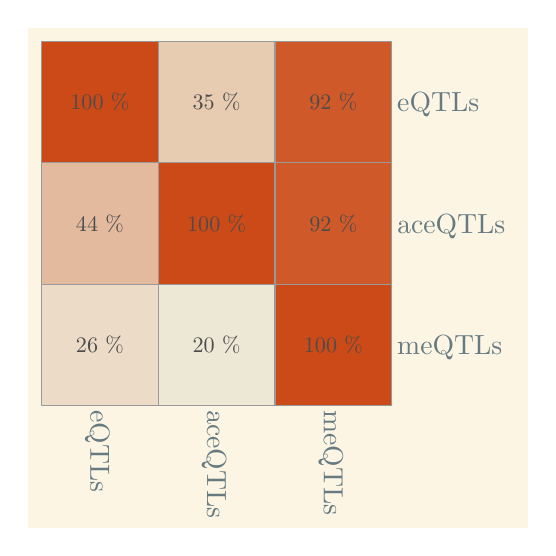
\begin{tikzpicture}[x=1pt,y=1pt]
\definecolor[named]{fillColor}{rgb}{0.99,0.96,0.89}
\path[use as bounding box,fill=fillColor] (0,0) rectangle (180.67,180.67);
\begin{scope}
\path[clip] (  0.00,  0.00) rectangle (180.67,180.67);
\definecolor[named]{drawColor}{rgb}{0.60,0.60,0.60}
\definecolor[named]{fillColor}{rgb}{0.80,0.29,0.09}

\path[draw=drawColor,line width= 0.4pt,line join=round,line cap=round,fill=fillColor] (  5.02,131.80) rectangle ( 47.20,175.66);
\definecolor[named]{fillColor}{rgb}{0.89,0.73,0.62}

\path[draw=drawColor,line width= 0.4pt,line join=round,line cap=round,fill=fillColor] (  5.02, 87.95) rectangle ( 47.20,131.80);
\definecolor[named]{fillColor}{rgb}{0.92,0.86,0.78}

\path[draw=drawColor,line width= 0.4pt,line join=round,line cap=round,fill=fillColor] (  5.02, 44.09) rectangle ( 47.20, 87.95);
\definecolor[named]{drawColor}{rgb}{0.30,0.30,0.30}

\node[text=drawColor,anchor=base,inner sep=0pt, outer sep=0pt, scale=  0.80] at ( 26.11,150.97) {100 \%};

\node[text=drawColor,anchor=base,inner sep=0pt, outer sep=0pt, scale=  0.80] at ( 26.11,107.12) {44 \%};

\node[text=drawColor,anchor=base,inner sep=0pt, outer sep=0pt, scale=  0.80] at ( 26.11, 63.26) {26 \%};
\definecolor[named]{drawColor}{rgb}{0.60,0.60,0.60}
\definecolor[named]{fillColor}{rgb}{0.91,0.80,0.70}

\path[draw=drawColor,line width= 0.4pt,line join=round,line cap=round,fill=fillColor] ( 47.20,131.80) rectangle ( 89.38,175.66);
\definecolor[named]{fillColor}{rgb}{0.80,0.29,0.09}

\path[draw=drawColor,line width= 0.4pt,line join=round,line cap=round,fill=fillColor] ( 47.20, 87.95) rectangle ( 89.38,131.80);
\definecolor[named]{fillColor}{rgb}{0.93,0.91,0.84}

\path[draw=drawColor,line width= 0.4pt,line join=round,line cap=round,fill=fillColor] ( 47.20, 44.09) rectangle ( 89.38, 87.95);
\definecolor[named]{drawColor}{rgb}{0.30,0.30,0.30}

\node[text=drawColor,anchor=base,inner sep=0pt, outer sep=0pt, scale=  0.80] at ( 68.29,150.97) {35 \%};

\node[text=drawColor,anchor=base,inner sep=0pt, outer sep=0pt, scale=  0.80] at ( 68.29,107.12) {100 \%};

\node[text=drawColor,anchor=base,inner sep=0pt, outer sep=0pt, scale=  0.80] at ( 68.29, 63.26) {20 \%};
\definecolor[named]{drawColor}{rgb}{0.60,0.60,0.60}
\definecolor[named]{fillColor}{rgb}{0.81,0.35,0.16}

\path[draw=drawColor,line width= 0.4pt,line join=round,line cap=round,fill=fillColor] ( 89.38,131.80) rectangle (131.56,175.66);

\path[draw=drawColor,line width= 0.4pt,line join=round,line cap=round,fill=fillColor] ( 89.38, 87.95) rectangle (131.56,131.80);
\definecolor[named]{fillColor}{rgb}{0.80,0.29,0.09}

\path[draw=drawColor,line width= 0.4pt,line join=round,line cap=round,fill=fillColor] ( 89.38, 44.09) rectangle (131.56, 87.95);
\definecolor[named]{drawColor}{rgb}{0.30,0.30,0.30}

\node[text=drawColor,anchor=base,inner sep=0pt, outer sep=0pt, scale=  0.80] at (110.47,150.97) {92 \%};

\node[text=drawColor,anchor=base,inner sep=0pt, outer sep=0pt, scale=  0.80] at (110.47,107.12) {92 \%};

\node[text=drawColor,anchor=base,inner sep=0pt, outer sep=0pt, scale=  0.80] at (110.47, 63.26) {100 \%};
\end{scope}
\begin{scope}
\path[clip] (  0.00,  0.00) rectangle (180.67,180.67);
\definecolor[named]{drawColor}{rgb}{0.40,0.48,0.51}

\node[text=drawColor,rotate=270.00,anchor=base west,inner sep=0pt, outer sep=0pt, scale=  1.00] at ( 22.67, 42.33) {eQTLs};

\node[text=drawColor,rotate=270.00,anchor=base west,inner sep=0pt, outer sep=0pt, scale=  1.00] at ( 64.85, 42.33) {aceQTLs};

\node[text=drawColor,rotate=270.00,anchor=base west,inner sep=0pt, outer sep=0pt, scale=  1.00] at (107.03, 42.33) {meQTLs};
\end{scope}
\begin{scope}
\path[clip] (  0.00,  0.00) rectangle (180.67,180.67);
\definecolor[named]{drawColor}{rgb}{0.40,0.48,0.51}

\node[text=drawColor,anchor=base west,inner sep=0pt, outer sep=0pt, scale=  1.00] at (133.53,150.29) {eQTLs};

\node[text=drawColor,anchor=base west,inner sep=0pt, outer sep=0pt, scale=  1.00] at (133.53,106.43) {aceQTLs};

\node[text=drawColor,anchor=base west,inner sep=0pt, outer sep=0pt, scale=  1.00] at (133.53, 62.58) {meQTLs};
\end{scope}
\end{tikzpicture}

        \vspace{-0.5cm}
    \end{column}
\end{columns}
\end{frame}

\tikzexternaldisable
\begin{frame}{Bayesian networks}
    \begin{itemize}
        \item Bayesian networks are directed graphical models, where the
            directed edges represent causal relationships
        \uncover<2-> {
        \item We use conditional Gaussian networks
        }
        \uncover<3-> {
        \item Score = likelihood of data given network
        }
    \end{itemize}
    \begin{center}
        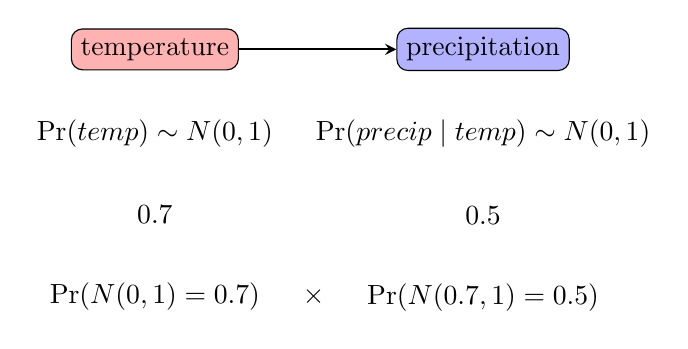
\begin{tikzpicture}
            \node [rectangle, rounded corners, draw, fill=red!30!white] 
            (t) {temperature};
            \node [rectangle, rounded corners, draw, fill=blue!30!white,
            right=2 of t] (p) {precipitation};
            \draw [->, >=stealth, thick] (t) -- (p);

            \uncover<2-> {
            \node [below=0.5 of t] (t1) {$\Pr(\text{temp}) \sim N(0, 1)$};
            \node [below=0.5 of p] (p1) {$\Pr(\text{precip} \mid \text{temp}) \sim N(0, 1)$};
            }

            \uncover<3-> {
            \node [below=0.5 of t1] (t2) {$0.7$};
            \node [below=0.5 of p1] (p2) {$0.5$};
            }

            \uncover<4-> {
            \node [below=0.5 of t2] (t3) {$\Pr(N(0, 1) = 0.7)$};
            \node [below=0.5 of p2] (p3) {$\Pr(N(0.7, 1) = 0.5)$};
            \path (t3) -- node {$\times$} (p3);
            }
        \end{tikzpicture}
    \end{center}
\end{frame}

\begin{frame}{Networks for QTLs}
    \begin{itemize}
        \item \textit{deal} and \textit{CGBayesNets} packages to construct one
            Bayesian network for each multi-QTL by exhaustive search
        \uncover<2->{
        \item With \textit{deal}, edges into genotype were blacklisted
        }\uncover<3->{
        \item Most common network structure was independence
        }\uncover<4->{
        \item Accounted for 42\% of \textit{deal} networks, 29\% of
            \textit{CGBayesNets} networks
        }
    \end{itemize}
    \begin{center}
        %       [g][e|g][ace|g][me|g] 101
%    [g][e|g][ace|e:me][me|g]  14
%      [g][e|g][ace|me][me|g]  13
%       [g][e|g][ace|e][me|g]  12
%      [g][e|me][ace|g][me|g]  12
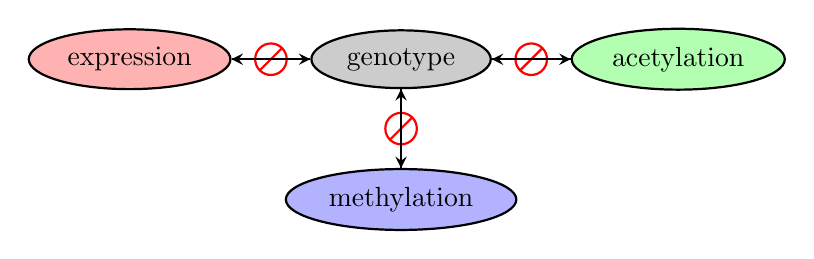
\begin{tikzpicture}
    [every node/.style={ellipse, draw, minimum width=8mm},
     every path/.style={->, >=stealth, thick, draw}]
    \node [fill=black!20!white] (g) {genotype};
    \node [fill=red!30!white, left=of g] (e) {expression};
    \node [fill=green!30!white, right=of g] (a) {acetylation};
    \node [fill=blue!30!white, below =of g] (m) {methylation};

    \uncover<2>{
        \draw (e) -- node [-, draw=red, minimum width=4mm, forbidden sign] { } (g);
        \draw (a) -- node [-, draw=red, minimum width=4mm, forbidden sign] { } (g);
        \draw (m) -- node [-, draw=red, minimum width=4mm, forbidden sign] { } (g);
    }

    \uncover<3->{
        \draw (g) -- (e);
        \draw (g) -- (a);
        \draw (g) -- (m);
    }
\end{tikzpicture}

    \end{center}
\end{frame}
\tikzexternalenable

\begin{frame}{Future Work}
    \begin{itemize}
        \item Expand the number of multi-QTLs
            \begin{itemize}
                \item More that just the best SNP per feature
                \item Identify overlapping QTLs intelligently
            \end{itemize}
        \item More rigourous criterion for number of PCs to remove
        \item Try other packages for network learning (HyPhy)
        \item Are QTLs enriched in SNPs identified in GWAS studies?
        \item Correlations with phenotype (cognitive decline etc.)
    \end{itemize}
\end{frame}

\begin{frame}{Thank you!}
    \begin{columns}
        \begin{column}{0.5\textwidth}
            \begin{itemize}
                \item All the bioinformatics students
                \item Sharon Ruschkowski
            \end{itemize}
        \end{column}
        \begin{column}{0.5\textwidth}
            \begin{center}
                \includegraphics[scale=0.3]{logos/test} \\
                \includegraphics[scale=0.2]{logos/bioinfo} \\
                \includegraphics[scale=0.2]{logos/ubc} \\
                \includegraphics[scale=0.1]{logos/nserc} \\
                \includegraphics[scale=0.2]{logos/cihr}
            \end{center}
        \end{column}
    \end{columns}
\end{frame}

\begin{frame}{Software}
    \begin{columns}
    \begin{column}{0.4\textwidth}
    \textbf{QTL analysis}
    \begin{itemize}
        \item
            \href{http://www.bios.unc.edu/research/genomic_software/Matrix_eQTL}
            {Matrix eQTL}
        \item
            \href{http://www.bioconductor.org/packages/release/bioc/html/qvalue.html}
            {qvalue}
    \end{itemize}
    \textbf{Bayesian networks}
    \begin{itemize}
        \item \href{http://cran.r-project.org/web/packages/deal/index.html}
                   {deal}
        \item \href{http://www.cgbayesnets.com}{CGBayesNets}
    \end{itemize}
    \end{column}
    \begin{column}{0.4\textwidth}
    \textbf{Slides}
    \begin{itemize}
        \item \href{http://www.ctan.org/pkg/beamer}{beamer}
        \item \href{https://www.ctan.org/pkg/pgf}{TikZ}
        \item
            \href{http://cran.r-project.org/web/packages/tikzDevice/index.html}
            {tikzDevice}
    \end{itemize}
    \textbf{Plots}
    \begin{itemize}
        \item \href{http://cran.r-project.org/web/packages/pheatmap/index.html}
                   {pheatmap}
        \item \href{http://ggplot2.org/}{ggplot2}
        \item
            \href{http://cran.r-project.org/web/packages/VennDiagram/index.html}
            {VennDiagram}
    \end{itemize}
    \textbf{Colour Scheme}
    \begin{itemize}
        \item \href{http://ethanschoonover.com/solarized}{solarized}
    \end{itemize}
    \end{column}
    \end{columns}
\end{frame}

\end{document}
